\documentclass[10pt,oneside]{book}


\usepackage{scalerel}

\usepackage[textwidth=1.5in]{todonotes}
\usepackage{clrscode3e}
\usepackage{hyperref}
\usepackage{comment}
\usepackage{appendix}

%%%%%%%%%%%%%%%%%%%%%%%%%%%%%%%%%%%%%%%%%%%%%%%%%%%%%%%%%%%%%%%%%%%%%%
% Structure
%%%%%%%%%%%%%%%%%%%%%%%%%%%%%%%%%%%%%%%%%%%%%%%%%%%%%%%%%%%%%%%%%%%%%%

% Don't put chapter number in section numbers
% \renewcommand*\thesection{\arabic{section}}	% commented out to include chapter number in section numbers

\newcommand{\anchorednote}[2]{ #1 \note{#2} }	% anchored note - needed for latex2edx
\newcommand{\note}[1]{\todo[color=blue!10,
  linecolor=blue!90,size=\small]{\linespread{0.9}\selectfont{#1}\par}}
\newcommand\lpknote[1]{\todo[color=orange!10, linecolor=orange!90,
  size=\footnotesize]{\linespread{0.9}\selectfont{{\bf LPK!!} #1}\par}}

\usepackage{tcolorbox}
\newtcolorbox{examplebox}{colback=green!5!white}
\newtcolorbox{noticebox}{colback=red!5!white}

% \scalebox{1.5}{\begin{tikzpicture}
%   % Put your tikz code here
% \end{tikzpicture}}

\newcommand\studyquestion[1]{\vskip0.05in\todo[inline, color=yellow!5]{{\bf
      Study Question:}  #1}}

\def\myrightmargin{2.0in}
% Make it compact for printing
%\renewcommand{\note}[1]{\footnote{#1}}
%\def\myrightmargin{1.0in}
\usepackage[left=1in, top=1in, bottom=1in,right=\myrightmargin]{geometry}
\usepackage{fancyhdr}
\usepackage[mmddyy,hhmmss]{datetime}
\pagestyle{fancy}
\lhead{\em MIT 6.390}
\chead{\em Fall 2023}
\rhead{\em \thepage} 
\rfoot{\em Last Updated: \today\ \currenttime}
\cfoot{}
%\markright{MIT 6.036 \hfill Fall 2020 \hfill}

\usepackage[Sonny]{fncychap}

\usepackage{listings}
% Provide compact itemize, etc.
\usepackage{paralist}

\setcounter{secnumdepth}{4}
\setcounter{tocdepth}{4}

\usepackage[shortlabels]{enumitem}

%%%%%%%%%%%%%%%%%%%%%%%%%%%%%%%%%%%%%%%%%%%%%%%%%%%%%%%%%%%%%%%%%%%%%%
% Fonts
%%%%%%%%%%%%%%%%%%%%%%%%%%%%%%%%%%%%%%%%%%%%%%%%%%%%%%%%%%%%%%%%%%%%%%

\usepackage{amsmath}
\usepackage{amsfonts}
\renewcommand{\rmdefault}{ppl} % rm is palatino
\linespread{1.05}        % Palatino needs more leading
\usepackage[scaled]{helvet} % ss
%\usepackage[scaled=1.03]{inconsolata}
\usepackage{courier} % Alternative to inconsolata
\usepackage{eulervm} 
\normalfont
%\usepackage[T1]{fontenc}
% bold symbols math mode
\usepackage{bm}
% blackboard bold
%\usepackage{bbold}
% Dangerous bend!  /dbend
%\usepackage{manfnt}

%%%%%%%%%%%%%%%%%%%%%%%%%%%%%%%%%%%%%%%%%%%%%%%%%%%%%%%%%%%%%%%%%%%%%%
% Math macros
%%%%%%%%%%%%%%%%%%%%%%%%%%%%%%%%%%%%%%%%%%%%%%%%%%%%%%%%%%%%%%%%%%%%%%

% Use to index over examples
\newcommand\ex[2]{#1^{(#2)}}
% Data sets
\newcommand\data{{\cal D}}
\newcommand\dataTrain{{\cal D}_n}
\newcommand\dataTest{{\cal D}_{n'}}
% Model, hypoth
\newcommand\model{{\cal M}}
\newcommand\hclass{{\cal H}}
% Max likelihood
\newcommand\ml[1]{#1_{\bf ml}}
% Empirical risk min
\newcommand\erm[1]{#1_{\bf erm}}
% Arg max
\newcommand\argmax[1]{{\rm arg}\max_{#1}}
\newcommand\argmin[1]{{\rm arg}\min_{#1}}
% Math
\newcommand{\R}{\mathbb{R}}
% errors
\newcommand{\trainerr}{\mathcal{E}_n}
\newcommand{\testerr}{\mathcal{E}}
\newcommand{\trainerrreg}{\text{MSE}_\text{train}}
\newcommand{\testerrreg}{\text{MSE}_\text{test}}
% sign
\newcommand{\sign}{\text{sign}}
% 2d vec
\newcommand*{\twodrow}[2]{\begin{bmatrix} #1 & #2 \end{bmatrix}}
\newcommand*{\twodcol}[2]{\begin{bmatrix} #1 \\ #2 \end{bmatrix}}
% norm
\newcommand{\norm}[1]{\left\lVert#1\right\rVert}
% alg
\newcommand{\alg}{\mathcal{A}}
% loss
\newcommand{\loss}{\mathcal{L}}


%%%%%%%%%%%%%%%%%%%%%%%%%%%%%%%%%%%%%%%%%%%%%%%%%%%%%%%%%%%%%%%%%%%%%%
% Math packages
%%%%%%%%%%%%%%%%%%%%%%%%%%%%%%%%%%%%%%%%%%%%%%%%%%%%%%%%%%%%%%%%%%%%%%
% Thm styles
\usepackage{amsthm}

\usepackage{mathtools}

%%%%%%%%%%%%%%%%%%%%%%%%%%%%%%%%%%%%%%%%%%%%%%%%%%%%%%%%%%%%%%%%%%%%%%
% Diagrams
%%%%%%%%%%%%%%%%%%%%%%%%%%%%%%%%%%%%%%%%%%%%%%%%%%%%%%%%%%%%%%%%%%%%%%

%\usepackage{xcolor}
\usepackage{tikz}
\usepackage{expl3}
\usepackage{caption}
\usepackage{float}
\ExplSyntaxOn
\int_zero_new:N \g__prg_map_int 
\ExplSyntaxOff
\usepackage{pgfplots}
\usetikzlibrary{calc}
\usetikzlibrary{decorations.pathreplacing,calligraphy}
\usetikzlibrary{arrows}
\usetikzlibrary{plotmarks}
\usetikzlibrary{automata, positioning}

% plus and minus macros
\tikzset{
  pluscs/.pic={
    \draw[ultra thick, blue] +(axis cs: -.2,0) -- +(axis cs: .2,0);
    \draw[ultra thick, blue] +(axis cs: 0,-.2) -- +(axis cs: 0,.2);
  },
  plus/.pic={
    \draw[ultra thick, blue] +(-.2,0) -- +(.2,0);
    \draw[ultra thick, blue] +(0,-.2) -- +(0,.2);
  },
  minus/.pic={
    \draw[ultra thick, red] +(-.2,0) -- +(.2,0);
  },
  plusblk/.pic={
    \draw[ultra thick] +(-.2,0) -- +(.2,0);
    \draw[ultra thick] +(0,-.2) -- +(0,.2);
  },
  minusblk/.pic={
    \draw[ultra thick] +(-.2,0) -- +(.2,0);
  },
}

% https://tex.stackexchange.com/questions/203821/draw-round-rectangular-bracket-embracing-nodes-in-tikz
\tikzset{
    ncbar angle/.initial=90,
    ncbar/.style={
        to path=(\tikztostart)
        -- ($(\tikztostart)!#1!\pgfkeysvalueof{/tikz/ncbar angle}:(\tikztotarget)$)
        -- ($(\tikztotarget)!($(\tikztostart)!#1!\pgfkeysvalueof{/tikz/ncbar angle}:(\tikztotarget)$)!\pgfkeysvalueof{/tikz/ncbar angle}:(\tikztostart)$)
        -- (\tikztotarget)
    },
    ncbar/.default=0.5cm,
}

\tikzset{square left brace/.style={ncbar=0.3cm}}
\tikzset{square right brace/.style={ncbar=-0.3cm}}

% other helpful definitions

\def\Xt{\tilde{X}}
\def\Yt{\tilde{Y}}


\newcounter{col}


%%% Local Variables:
%%% mode: latex
%%% TeX-master: "top"
%%% End:


\usepackage{amsmath,amsthm,amssymb,graphicx,mathtools,tikz,hyperref,mathdots}

\usepackage[normalem]{ulem}

%Not sure of any special consequences - used to fix \mathbb{1}
\usepackage[bb=dsserif]{mathalpha}

\usetikzlibrary{positioning}
\newcommand{\n}{\mathbb{N}}
\newcommand{\z}{\mathbb{Z}}
\newcommand{\q}{\mathbb{Q}}
\newcommand{\cx}{\mathbb{C}}
\newcommand{\real}{\mathbb{R}}
\newcommand{\field}{\mathbb{F}}
\newcommand{\ita}[1]{\textit{#1}}
\newcommand{\com}[2]{#1\backslash#2}
\newcommand{\oneton}{\{1,2,3,...,n\}}
\newcommand\idea[1]{\begin{gather*}#1\end{gather*}}
\newcommand\ef{\ita{f} }
\newcommand\eff{\ita{f}}
\newcommand\proofs[1]{\begin{proof}#1\end{proof}}
\newcommand\inv[1]{#1^{-1}}
\newcommand\setb[1]{\{#1\}}
\newcommand\en{\ita{n }}
\newcommand{\vbrack}[1]{\langle #1\rangle}





\newenvironment{drytheorem}[2][dryTheorem]{\begin{trivlist}
\item[\hskip \labelsep {\bfseries #1}\hskip \labelsep {\bfseries #2.}]}{\end{trivlist}}
\newenvironment{drylemma}[2][dryLemma]{\begin{trivlist}
\item[\hskip \labelsep {\bfseries #1}\hskip \labelsep {\bfseries #2.}]}{\end{trivlist}}
\newenvironment{dryexercise}[2][dryExercise]{\begin{trivlist}
\item[\hskip \labelsep {\bfseries #1}\hskip \labelsep {\bfseries #2.}]}{\end{trivlist}}
\newenvironment{dryreflection}[2][dryReflection]{\begin{trivlist}
\item[\hskip \labelsep {\bfseries #1}\hskip \labelsep {\bfseries #2.}]}{\end{trivlist}}
\newenvironment{dryproposition}[2][dryProposition]{\begin{trivlist}
\item[\hskip \labelsep {\bfseries #1}\hskip \labelsep {\bfseries #2.}]}{\end{trivlist}}
\newenvironment{drycorollary}[2][dryCorollary]{\begin{trivlist}
\item[\hskip \labelsep {\bfseries #1}\hskip \labelsep {\bfseries #2.}]}{\end{trivlist}}
 \hypersetup{
 colorlinks,
 linkcolor=blue
 }
 
%Used for arbitrary-sized curly braces
\newcommand{\biggglB}[1]{\left\{\!\parbox{0pt}{\rule{0pt}{#1}}\right.}
\newcommand{\bigggrB}[1]{\left.\parbox{0pt}{\rule{0pt}{#1}}\!\right\}}
 
 
\newcommand*\circled[1]{\tikz[baseline=(char.base)]{
            \node[shape=circle,draw,inner sep=2pt] (char) {#1};}}
 
\newcommand\overmat[2]{%
  \makebox[0pt][l]{$\smash{\color{white}\overbrace{\phantom{%
    \begin{matrix}#2\end{matrix}}}^{\text{\color{black}#1}}}$}#2}
\newcommand\bovermat[2]{%
  \makebox[0pt][l]{$\smash{\overbrace{\phantom{%
    \begin{matrix}#2\end{matrix}}}^{\text{#1}}}$}#2}
 
 
 
% \newcommand\iddots{\mathinner{
%   \kern1mu\raise1pt{.}
%   \kern2mu\raise4pt{.}
%   \kern2mu\raise7pt{\Rule{0pt}{7pt}{0pt}.}
%   \kern1mu
% }} 
 

%%Shaunticlair's own macros
 
\newcommand{\deriv}[2]{\frac{\dd #1}{\dd #2}}
\newcommand{\dderiv}[2]{\frac{\dd^2 #1}{\dd #2^2} }

\newcommand{\derivslash}[2]{{\dd #1}/{\dd #2}}
\newcommand{\pderivslash}[2]{{\partial #1}/{\partial #2}}


\newcommand{\pderiv}[2]{\frac{\partial #1}{\partial #2}}
\newcommand{\pdderiv}[2]{\frac{\partial^2 #1}{\partial #2^2}}

\newcommand{\bigderiv}[2]{\dfrac{\dd #1}{\dd #2}}
\newcommand{\bigpderiv}[2]{\dfrac{\partial #1}{\partial #2}}

\usepackage{parskip, physics, enumitem}

\definecolor{betterpurple}{HTML}{7F00FF}
\definecolor{darkbrown}{HTML}{964b00}
\definecolor{easypink}{HTML}{ff607f}
\definecolor{darkgray}{HTML}{6b7283}
\definecolor{darkgreen}{HTML}{008600}
\definecolor{brownbrown}{HTML}{A4711E}
\definecolor{teal}{HTML}{008080}
\definecolor{vlightblue}{HTML}{00d2ff}

\newcommand{\org}[1]{\textcolor{orange}{#1}}
\newcommand{\pur}[1]{\textcolor{betterpurple}{#1}}
\newcommand{\red}[1]{\textcolor{red}{#1}}
\newcommand{\blu}[1]{\textcolor{blue}{#1}}
\newcommand{\bro}[1]{\textcolor{darkbrown}{#1}}
\newcommand{\pin}[1]{\textcolor{easypink}{#1}}
\newcommand{\gre}[1]{\textcolor{darkgray}{#1}}
\newcommand{\grn}[1]{\textcolor{green!70!black}{#1}}
\newcommand{\tea}[1]{\textcolor{teal}{#1}}
\newcommand{\bru}[1]{\textcolor{brownbrown}{#1}}
\newcommand{\lbl}[1]{\textcolor{vlightblue}{#1}}

\newcommand{\orgg}[1]{\textbf{\textcolor{orange}{#1}}}
\newcommand{\redd}[1]{\textbf{\textcolor{red}{#1}}}
\newcommand{\gren}[1]{\textbf{\textcolor{green!70!black}{#1}}}
\newcommand{\brow}[1]{\textbf{\textcolor{darkbrown}{#1}}}
\newcommand{\purp}[1]{\textbf{\textcolor{betterpurple}{#1}}}
\newcommand{\brun}[1]{\textbf{\textcolor{brownbrown}{#1}}}
\newcommand{\pink}[1]{\textbf{\textcolor{easypink}{#1}}}
\newcommand{\lblu}[1]{\textbf{\textcolor{vlightblue}{#1}}}



\newcommand{\miniex}[0]{\purp{Example: }}
\newcommand{\nth}[1]{ #1^{ \text{th} } }

\newcommand{\In}[0]{\textbf{in }}

\newcommand{\rgi}[0]{ \red{\ex{g}{i}} }

\newcommand{\exi}[0]{ \ex{x}{i} }
\newcommand{\eyi}[0]{ \ex{y}{i} }

\newcommand{\rxi}[0]{ \red{\exi }}
\newcommand{\ryi}[0]{ \red{\eyi }}

\newcommand{\bxi}[0]{ \blu{\exi }}
\newcommand{\byi}[0]{ \blu{\eyi }}

\newcommand{\cmul}[0]{\; \cdot \;}

\newcommand{\secdiv}[0]{\centerline{\uwave{\uwave{\hspace{14cm}}}}}
\newcommand{\subsecdiv}[0]{\centerline{\uwave{\uwave{\hspace{10cm}}}}}
%\newcommand{\boxdiv}[0]{\centerline{\rule{10cm}{1pt}}}

\newcommand{\boxdiv}[0]{\centerline{\uwave{\uwave{\hspace{10cm}}}}}

\newcommand{\setty}[1]{\Bigl\{#1\Bigr\}}
\newcommand{\prob}[1]{ \mathbf{P} \Bigl\{#1\Bigr\}}
\newcommand{\given}[2]{ \mathbf{P} \Bigl\{#1 \;\; \Big| \;\; #2 \Bigr\}}

\newcommand{\smashedoverbrace}[2]{\smash{\overbrace{#1}^{#2}}\vphantom{#1}}
\newcommand{\smashedunderbrace}[2]{\smash{\underbrace{#1}_{#2}}\vphantom{#1}}

% \newcommand{\loss}[0]{\mathcal{L}}

%%% Local Variables:
%%% mode: latex
%%% TeX-master: "top"
%%% End:

\newcommand{\cbrt}[1]{\sqrt[3]{#1}}
\newcommand{\floor}[1]{\left\lfloor #1 \right\rfloor}
\newcommand{\ceiling}[1]{\left\lceil #1 \right\rceil}
\newcommand{\mailto}[1]{\href{mailto:#1}{\texttt{#1}}}
\newcommand{\ol}{\overline}
\newcommand{\ul}{\underline}
\newcommand{\wt}{\widetilde}
\newcommand{\wh}{\widehat}
\newcommand{\eps}{\varepsilon}
%\renewcommand{\iff}{\Leftrightarrow}
%\renewcommand{\implies}{\Rightarrow}
\newcommand{\vocab}[1]{\textbf{\color{blue} #1}}
\newcommand{\catname}{\mathsf}
\newcommand{\hrulebar}{
  \par\hspace{\fill}\rule{0.95\linewidth}{.7pt}\hspace{\fill}
  \par\nointerlineskip \vspace{\baselineskip}
}
\newcommand{\half}{\frac{1}{2}}

%More commands and math operators
\DeclareMathOperator{\cis}{cis}
\DeclareMathOperator*{\lcm}{lcm}
%\DeclareMathOperator*{\argmin}{arg min}
%\DeclareMathOperator*{\argmax}{arg max}

%Convenient Environments
\newenvironment{soln}{\begin{proof}[Solution]}{\end{proof}}
\newenvironment{parlist}{\begin{inparaenum}[(i)]}{\end{inparaenum}}
\newenvironment{gobble}{\setbox\z@\vbox\bgroup}{\egroup}

%Inequalities
\newcommand{\cycsum}{\sum_{\mathrm{cyc}}}
\newcommand{\symsum}{\sum_{\mathrm{sym}}}
\newcommand{\cycprod}{\prod_{\mathrm{cyc}}}
\newcommand{\symprod}{\prod_{\mathrm{sym}}}

%From H113 "Introduction to Abstract Algebra" at UC Berkeley
\newcommand{\CC}{\mathbb C}
\newcommand{\FF}{\mathbb F}
\newcommand{\NN}{\mathbb N}
\newcommand{\QQ}{\mathbb Q}
\newcommand{\RR}{\mathbb R}
\newcommand{\ZZ}{\mathbb Z}
\newcommand{\charin}{\text{ char }}
% \DeclareMathOperator{\sign}{sign}
\DeclareMathOperator{\Aut}{Aut}
\DeclareMathOperator{\Inn}{Inn}
\DeclareMathOperator{\Syl}{Syl}
\DeclareMathOperator{\Gal}{Gal}
\DeclareMathOperator{\GL}{GL} % General linear group
\DeclareMathOperator{\SL}{SL} % Special linear group

%From Kiran Kedlaya's "Geometry Unbound"
% \newcommand{\abs}[1]{\left\lvert #1 \right\rvert}
% \newcommand{\norm}[1]{\left\lVert #1 \right\rVert}
\newcommand{\dang}{\measuredangle} %% Directed angle
\newcommand{\ray}[1]{\overrightarrow{#1}}
\newcommand{\seg}[1]{\overline{#1}}
\newcommand{\arc}[1]{\wideparen{#1}}

%From M275 "Topology" at SJSU
% \newcommand{\id}{\mathrm{id}}
\newcommand{\taking}[1]{\xrightarrow{#1}}
% \newcommand{\inv}{^{-1}}

%From M170 "Introduction to Graph Theory" at SJSU
\DeclareMathOperator{\diam}{diam}
\DeclareMathOperator{\ord}{ord}
%\newcommand{\defeq}{\overset{\mathrm{def}}{=}}
\newcommand{\defeq}{\coloneqq}

%From the USAMO .tex filse
\newcommand{\st}{^{\text{st}}}
\newcommand{\nd}{^{\text{nd}}}
\renewcommand{\th}{^{\text{th}}}
\newcommand{\dg}{^\circ}
\newcommand{\ii}{\item}

% From Math 55 and Math 145 at Harvard
\newenvironment{subproof}[1][Proof]{%
\begin{proof}[#1] \renewcommand{\qedsymbol}{$\blacksquare$}}%
{\end{proof}}

\newcommand{\liff}{\leftrightarrow}
\newcommand{\lthen}{\rightarrow}
\newcommand{\opname}{\operatorname}
\newcommand{\surjto}{\twoheadrightarrow}
\newcommand{\injto}{\hookrightarrow}
\newcommand{\On}{\mathrm{On}} % ordinals
\DeclareMathOperator{\img}{im} % Image
\DeclareMathOperator{\Img}{Im} % Image
\DeclareMathOperator{\coker}{coker} % Cokernel
\DeclareMathOperator{\Coker}{Coker} % Cokernel
\DeclareMathOperator{\Ker}{Ker} % Kernel
% \DeclareMathOperator{\rank}{rank}
\DeclareMathOperator{\Spec}{Spec} % spectrum
% \DeclareMathOperator{\Tr}{Tr} % trace
\DeclareMathOperator{\pr}{pr} % projection
\DeclareMathOperator{\ext}{ext} % extension
\DeclareMathOperator{\pred}{pred} % predecessor
\DeclareMathOperator{\dom}{dom} % domain
\DeclareMathOperator{\ran}{ran} % range
\DeclareMathOperator{\Hom}{Hom} % homomorphism
% \DeclareMathOperator{\End}{End} % endomorphism

% Things Lie
\newcommand{\kg}{\mathfrak g}
\newcommand{\kh}{\mathfrak h}
\newcommand{\kn}{\mathfrak n}
\newcommand{\ku}{\mathfrak u}
\newcommand{\kz}{\mathfrak z}
\DeclareMathOperator{\Ext}{Ext} % Ext functor
\DeclareMathOperator{\Tor}{Tor} % Tor functor

% More script letters etc.
\newcommand{\SA}{\mathscr A}
\newcommand{\SB}{\mathscr B}
\newcommand{\SC}{\mathscr C}
\newcommand{\SD}{\mathscr D}
\newcommand{\SF}{\mathscr F}
\newcommand{\SG}{\mathscr G}
\newcommand{\SH}{\mathscr H}
\newcommand{\OO}{\mathcal O}


%%fakesection Napkin Macros
\newcommand{\Zc}[1]{\ZZ/#1\ZZ}
\newcommand{\Zcc}[1]{\ZZ/(#1)\ZZ}
\newcommand{\Zm}[1]{(\ZZ/#1\ZZ)^\times}
\newcommand{\EE}{\mathbb E}
\newcommand{\TT}{\mathbb T}
\newcommand{\im}{^{\text{img}}} % or ``?
\newcommand{\pre}{^{\text{pre}}}
\newcommand{\normalin}{\trianglelefteq}
\newcommand{\triv}{\mathrm{triv}}
\newcommand{\largeotimes}[1]{\mathop{\otimes}\limits_{#1}}
\newcommand{\Mat}{\mathrm{Mat}}
\newcommand{\PGL}[1]{\mathbf{PGL}_{#1}(\CC)}

\DeclareMathOperator{\Stab}{Stab}
\DeclareMathOperator{\FixPt}{FixPt}
\DeclareMathOperator{\refl}{refl}
\DeclareMathOperator{\Fun}{Fun}
\DeclareMathOperator{\Irrep}{Irrep}
% \DeclareMathOperator{\Res}{Res}
\DeclareMathOperator{\Reg}{Reg}
\DeclareMathOperator{\Classes}{Classes}
\DeclareMathOperator{\Frac}{Frac}
\newcommand{\FunCl}{\Fun_{\mathrm{class}}}
\newcommand{\Homrep}{\Hom_{\mathrm{rep}}}
\newcommand{\ab}{^\text{ab}} % abelianization
% \DeclareMathOperator{\ev}{ev}
\DeclareMathOperator{\Wind}{\mathbf I}
\newcommand{\Ctriv}{\CC_{\mathrm{triv}}}
\newcommand{\Csign}{\CC_{\mathrm{sign}}}

% Alg geom macros
\newcommand{\VV}{\mathcal V}
\newcommand{\Vp}{\mathcal V_{\text{pr}}}
\newcommand{\Aff}{\mathbb A}
\newcommand{\II}{\mathcal I_{\text{rad}}}
\newcommand{\RP}{\mathbb{RP}}
\newcommand{\CP}{\mathbb{CP}}
\newcommand{\Cl}{\mathrm{Cl}}
\newcommand{\restrict}[1]{\bgroup\restriction_{#1}\egroup}
\DeclareMathOperator{\Opens}{OpenSets}
\DeclareMathOperator{\Proj}{Proj}
\DeclareMathOperator{\res}{res}
\newcommand{\km}{\mathfrak m}
\newcommand{\sh}{^\mathrm{sh}}

\renewcommand{\Re}{\opname{Re}}
\renewcommand{\Im}{\opname{Im}}

%% Category Theory macros
\renewcommand{\AA}{\mathcal A}
\newcommand{\BB}{\mathcal B}
\newcommand{\obj}{\operatorname{obj}}
% \newcommand{\op}{^{\mathrm{op}}}


\usepackage{tkz-graph}
\pgfarrowsdeclare{biggertip}{biggertip}{%
  \setlength{\arrowsize}{1pt}
  \addtolength{\arrowsize}{.1\pgflinewidth}
  \pgfarrowsrightextend{0}
  \pgfarrowsleftextend{-5\arrowsize}
}{%
  \setlength{\arrowsize}{1pt}
  \addtolength{\arrowsize}{.1\pgflinewidth}
  \pgfpathmoveto{\pgfpoint{-5\arrowsize}{4\arrowsize}}
  \pgfpathlineto{\pgfpointorigin}
  \pgfpathlineto{\pgfpoint{-5\arrowsize}{-4\arrowsize}}
  \pgfusepathqstroke
}
\tikzset{
	EdgeStyle/.style = {>=biggertip}
}

\usepackage[all,cmtip,2cell]{xy}
\UseTwocells
\newcommand\nattfm[5]{\xymatrix@C+2pc{#1 \rtwocell<4>^{#2}_{#4}{\; #3} & #5}}

%% Alg Top macros
\DeclareMathOperator{\Cells}{Cells}
\newcommand{\HdR}{H_{\mathrm{dR}}}

%% Alg NT macros
\newcommand{\ka}{\mathfrak a}
\newcommand{\kb}{\mathfrak b}
\newcommand{\kp}{\mathfrak p}
\newcommand{\kq}{\mathfrak q}

\newcommand{\Frob}{\mathrm{Frob}}
\DeclareMathOperator{\Norm}{N}
\DeclareMathOperator{\Ram}{Ram}
\newcommand{\TrK}{\Tr_{K/\QQ}}
\newcommand{\NK}{\Norm_{K/\QQ}}
\newcommand{\kf}{\mathfrak f}
\newcommand{\kP}{\mathfrak P}
\newcommand{\kQ}{\mathfrak Q}

%% Diff geo macros
\newcommand{\ee}{\mathbf e}
\newcommand{\fpartial}[2]{\frac{\partial #1}{\partial #2}}

%% ST macros
\newcommand{\CH}{\mathsf{CH}}
\newcommand{\ZFC}{\mathsf{ZFC}}

\newcommand{\Name}{\text{Name}}
\newcommand{\Po}{\mathbb P}
\newcommand{\nrank}{\opname{n-rank}} % ranks
\newcommand{\PP}{\mathcal P}

\newcommand{\EmptySet}{\mathrm{EmptySet}}
\newcommand{\PowerSet}{\mathrm{PowerSet}}
\newcommand{\Pairing}{\mathrm{Pairing}}
\newcommand{\Infinity}{\mathrm{Infinity}}
\newcommand{\Extensionality}{\mathrm{Extensionality}}
\newcommand{\Foundation}{\mathrm{Foundation}}
\newcommand{\Union}{\mathrm{Union}}
\newcommand{\Comprehension}{\mathrm{Comprehension}}
\newcommand{\Replacement}{\mathrm{Replacement}}

\usepackage{mathrsfs}

\newcommand\MM{\mathscr M}
\newcommand\llex{<_{\text{lex}}}

\DeclareMathOperator{\cof}{cof}

%% Quantum macros
\usepackage{braket}
\newcommand{\cvec}[1]{\begin{bmatrix} #1 \end{bmatrix}}
\newcommand{\pair}[2]{\begin{bmatrix} #1 \\ #2 \end{bmatrix}}
\newcommand{\zup}{\ket\uparrow}
\newcommand{\zdown}{\ket\downarrow}
\newcommand{\xup}{\ket\rightarrow}
\newcommand{\xdown}{\ket\leftarrow}
\newcommand{\yup}{\ket\otimes}
\newcommand{\ydown}{\ket\odot}
\newcommand{\UCNOT}{U_{\mathrm{CNOT}}}
\newcommand{\UQFT}{U_{\mathrm{QFT}}}

%% Measure
\DeclareMathOperator{\Var}{Var}
\newcommand{\cme}{^\text{cm}}
\newcommand{\asto}{\xrightarrow{\text{a.s.}}}

%% Hot chili peppers
%\reversemarginpar
%\newcommand{\prechili}{\vspace*{0.3em}\hspace*{1.5em}}
%\newcommand{\nochili}{\hspace*{1.5em}}
%\newcommand{\chili}{\includegraphics[width=1.5em]{media/chili.png}}
%\newcommand{\gim}{\marginpar{\prechili\nochili\nochili\chili}}
%\newcommand{\yod}{\marginpar{\prechili\nochili\chili\chili}}
%\newcommand{\kurumi}{\marginpar{\prechili\chili\chili\chili}}

\usepackage{macros/lindrew}
\usepackage{subfigure}

\title{Explanatory Notes for 6.390}
\author{Shaunticlair Ruiz (Current TA)}
\date{Fall 2022}

\begin{document}
\maketitle

\setcounter{tocdepth}{1} %Needed or the TOC would be an essay...
\tableofcontents

%%First section of course: base concepts

% 
\setcounter{chapter}{-1} %Makes the prereq chapter chapter 0

\chapter{Prerequisites - Explanatory Notes}
\label{prerequisites}



    
This course assumes knowledge of several topics. Here, we'll outline them: hopefully, this will make it easier to get up to speed if you have a gap in your background, and to know what you're looking for.

This is designed to be somewhat comprehensive, so if you've taken a class, you can likely skip the corresponding section.

If a class has its own prerequisite, then we assume the understanding of that class as well. For example, we assume you know multi-variable calculus, so single-variable is assumed as well.
    
\section{Multi-variable Calculus (MIT's 18.02)}

    You will need most of the differential aspects of multi-variable calculus: 
    
    \begin{itemize}
        \item The concept of partial derivatives and how to find them
        \item The \textbf{multivariable} chain rule
        \item An intuition for the gradient as the \textbf{direction} of greatest increase in a function, and the \textbf{magnitude} of that increase.
    \end{itemize}
    
    It is helpful to able to visualize a surface created by a function. You won't need to memorize the shapes of specific surfaces; just the 3D intuition in general.
    
    You should also be able to imagine "zooming in" to that surface, and seeing it "locally" as a \textbf{plane}, just like how we zoom in to a one-variable function, and see the \textbf{tangent line}.
    
    Sometimes, in this class, we will also do derivatives \textbf{numerically}, where we approximate the derivative with finite steps, of the form
    
    \begin{equation}
        \deriv{y}{x} \approx \frac{ \Delta y}{ \Delta x}
    \end{equation}
    
    You should also be comfortable with some basic ideas of "infinity": what happens in the "limit as we approach infinity", for example.
    
    %Might want to add a visual for this
    
    You will not need double/triple/line integrals, curl, divergence, or greens/stokes theorem.
    
\section{Vectors and Matrices (MIT's 18.02)}

    You will need an understanding of vectors:
    \begin{itemize}
        \item You need to know what a vector is, with two interpretations:
            \begin{itemize}
                \item an \textbf{ordered list} of numbers
                \item an object in some "space" with \textbf{magnitude} and \textbf{direction}
            \end{itemize}
        
        \item You should know that the \textbf{length} or \textbf{dimension} of a vector is just how many numbers(or \textbf{elements}) that vector contains.
        
        \item You should know that a \textbf{scalar} is just a number, or in some perspectives, a 1-element vector.
        
        \item You need to be able to \textbf{add} or \textbf{subtract} pairs of vectors. You should also be able to \textbf{scale} them (in other words, multiply by a \textbf{scalar}).
        
        \item You should know how to take the \textbf{derivative} of a vector $\vec{v}$, with respect to a scalar $x$, in the form
        
        \begin{equation}
            \deriv{\vec{v}}{x}
        \end{equation}
    \end{itemize}
    
    You will also need to understand the \textbf{dot product}, and its intuition as the \textbf{similarity} between vectors.
    
    You will need to understand matrices:
    
    \begin{itemize}
        \item You should know what a matrix is, with three perspectives: 
        %Pictures, maybe?
            \begin{itemize}
                \item a 2D grid of numbers (in a "rectangle")
                \item an \textbf{ordered list} of equal-length vectors.
                \item a \textbf{transformation} of vectors.
            \end{itemize}
        
        \item You should understand the \textbf{dimensions} of a matrix, and the common notation  (\# of rows $\cross$ \# of columns)
        
        \item You need to be able to multiply two matrices, or a matrix times a vector.
            \begin{itemize}
                \item You need to understand when you are able to multiply matrices, based on dimensions.
                \item The dimensions of the new matrix after multiplication.
                \item How to do the calculation of multiplying matrices by hand.
            \end{itemize}
    \end{itemize}
    
    You should understand the \textbf{determinant}: both how to calculate it, and the intuition behind it.
    
    Finally, you should know what a matrix \textbf{inverse} is, and that a \textbf{zero-determinant} matrix has \textbf{no inverse}.
    
    
\section{Linear Algebra (18.06)}

    Currently, linear algebra is a \textbf{new} prerequisite.
    
    You need all of the concepts mentioned in the "vectors and matrices" segment.

    You should also understand \vocab{independence} between vectors, the \vocab{rank} of a matrix, and how to take the \vocab{transpose} of a matrix. 
    
    \vocab{Linearity} is a really nice (and important!) property , where a function doesn't get in the way of some simple operations: \textbf{addition} or \textbf{scalar multiplication}. The order doesn't matter.\\
    
        \begin{definition}
            For \vocab{linear} function/operator $\mathbb{L}$,
            
            \purp{Addition} (of any kind) has the same effect, before or after the function.
            
            \begin{equation*}
                \mathbb{L}(x+y) = \mathbb{L}(x) + \mathbb{L}(y)
            \end{equation*}
            
            \purp{Multiplication} by a \textbf{scalar} also has the same effect.
            
            \begin{equation*}
                \mathbb{L}(3z) = 3\mathbb{L}(z)
            \end{equation*}
            
        \end{definition}
    
    \miniex The \textbf{derivative} is \textbf{linear}: 
    
        \begin{equation}
            \deriv{}{x}[f+g] = \deriv{}{x}[f]+\deriv{}{x}[g]
        \end{equation}
        \begin{equation}
            \deriv{}{x}[10h]=10\deriv{}{x}[h]
        \end{equation}
    
    Often, we talk about \vocab{operators}. They're like functions, where they have an input and an output. But sometimes, we use this word when we have \textbf{another} function as an input.\\
    
        \begin{definition}
            An \vocab{operator} \textit{often} takes in a \purp{function} as an input, and gives another \purp{function} as an output.
        \end{definition}
        
        
        \note{An operator doesn't have a really "unique" definition in math: it's used for convenience.} 
    
    \miniex The \textbf{derivative} is also an \textbf{operator}. If you input $f(x) = x^2$, the output is $\deriv{}{x}[f(x)]=2x$: another \textbf{function}.
    
    Thus, we can call the derivative a \textbf{linear operator}.
    
    
    The \textbf{visual} intuition of a matrix as a spatial transformation is useful in this class. 
    \note{A good reference for intuition is the linear algebra series by YouTube channel, 3blue1brown! Each video averages 11 minutes, and has been helpful for many past students.}
    
    It would be helpful to understand \textbf{nullspace}, \textbf{column space}, and \textbf{vector spaces} in general.
    
\section{Programming (6.100A, 6.1010)}
    
    \textbf{For 6.100A:}
    
    You should be familiar with object-oriented programming in \textbf{Python}: you will be implementing various classes and simple algorithms in this class.
    
    You should have a basic understanding of \textbf{time complexity} and big-O notation. Ease with reading basic pseudocode would be helpful as well.
    
    
    
    \textbf{For 6.1010:}
    
    Either 6.1010 or 6.1210 are counted as a prereq: they are not equivalent, and neither is individually required to understand the course, but either will make your work in this class much easier.
    
    6.1010 offers more coding experience, which makes the process of implementation much smoother.
    
    \textbf{Misc:}
    
    Prior understanding of numpy is not mandatory, but would be very helpful. Pytorch would also be helpful, but is not used until much later in the course.
    
\section{Algorithms (6.1210)}
    
    Either 6.1010 or 6.1210 are counted as a prereq: they are not equivalent, and neither is individually required to understand the course, but either will make your work in this class much easier.
    
    6.1210 is about \textbf{algorithms}, and thus makes it easier to understand our discussions of different algorithms thoroughout this class.
    
    Concepts of dynamic programming, complexity, and reading/writing pseudocode are all helpful for this course.

\section{Probability}

    You don't need to have taken a full probability course, but there are some core concepts you must understand:
    
    \begin{itemize}
        \item \vocab{Probability} (or chance) is the relative \textbf{frequency} of a particular outcome, if you were to run many trials - specifically, it is the proportion of those trials that gave this particular outcome.
        
        For example, if $p=.4$, then you should expect to have that event occur 40 times for every 100, on average.
        
        \item Probabilities $p$ are between 0 and 1: 
            \begin{itemize}
                \item If $p=0$, the event \textbf{will not} occur%\note{In most cases. There are some strange exceptions.}
                \item If $p=1$, the event \textbf{will definitely} occur.
                \item If $p=.5$, the event has a 50\% chance of happening if you try once.
                \item Any other probability between 0 and 1 will give some corresponding percentile chance of occurring ($100*p\%$)
            \end{itemize}
            
        \item You can represent probability of event $A$ as
        
            \begin{equation}
                P(A)
            \end{equation}
            
            Treating $P$ as a function that returns the \textbf{probability}.
        
        \item If you want two events to both occur, you can write that with an \vocab{and} statement:
        
            \begin{equation}
                P(A \text{ and } B) = P(A \cap B)
            \end{equation}
            
        \item If you want at least one of two events to occur, you can write that with an \vocab{or} statement:
        
            \begin{equation}
                P(A \text{ or } B) = P(A \cup B)
            \end{equation}
            
        \item The \vocab{conditional probability} is the probability of an event \vocab{given} that another event has already occured:
        % If you know one event has occurred, and you want the chance of the other event, you can write that as a \vocab{given} statement:
        
            \begin{equation}
                P(B|A)
            \end{equation}
            
        This is read as "The probability of B \textbf{given} A".
        % , meaning, the probability of event B \textbf{if} event A is already known to have happened.
        
        \item Two events are \vocab{independent} if knowing the outcome of one event does not affect the odds of another. You can write this as 
        
            \begin{equation}
                P(A|B)P(B)=P(A \text{ and } B)
            \end{equation}
            
            You can equivalently use the next bullet point's definition.
        
        \item The chance of two \textbf{independent} events both happening is their odds multiplied.
            \begin{equation}
                P(A \text{ and } B) = P(A)P(B)
            \end{equation}
            
            
        \item The \vocab{sum} of the probabilities of all outcomes \textbf{must add} to 1: otherwise, there's a chance of getting none of the listed outcomes.
        
        \item The chance of a particular event not occurring is called the \vocab{complement}, and has a chance of $1-p$.
        
        
            
    \end{itemize}
    
\section{Notation: Sets}

    There are some common definitions and notations you should be familiar with (though they may be introduced if necessary).
    
    If you understand an equation, move on to the next one: each explanation is mostly basic.\\
    
    \begin{definition}
        An \vocab{element} is a single object in a collection of objects.
    \end{definition}
    
    This definition is often linked to \textbf{sets}.\\
    
    \begin{definition}
        A \vocab{set} is a collection of distinct elements with no given order: if you shuffle the elements in a different order, you have the same set.
    \end{definition}
    
    
    \begin{itemize}
        \item We can \vocab{define} a set by listing out its elements. For example, this says, "The set A contains the numbers 1, 2, and 3"
            \begin{equation}
                A = \{1, 2, 3\}
            \end{equation}
            
            
            
        \item Shows that an element is \vocab{in} a set. The following says "x is an element of the set $A$".
            \begin{equation}
                x \in A
            \end{equation}
            
        \item Shows that an element is \vocab{ not in} a set. The following says "x is \textbf{not} an element of the set $A$".
            \begin{equation}
                x \notin A
            \end{equation}
            
        \item \vocab{Natural numbers}, or the counting numbers. 
            \begin{equation}
                \mathbb{N} = \{ 1, 2, 3, 4, 5... \}
            \end{equation}
            
        \item \vocab{Real numbers}, or all of the numbers on the number line (include those between integers).
        
            \begin{equation}
                \mathbb{R}
            \end{equation}
            
        \item We can also define a set by starting with another set, and then listing a \vocab{restriction}:
        
            The following says, "Include each natural number $n$".
            
            \begin{equation}
                \{ n \in \n \}
            \end{equation}
            
            This seems redundant, but now, we can choose to only include natural numbers \textbf{larger than 10}:
            
            \begin{equation}
                \{ n \in \n \,|\, n > 10 \} = \{11, 12, 13, 14...\}
            \end{equation}
            
        % \item \vocab{Subsets} are used when one set contains every element of another set. 
        \item A set $A$ is a \vocab{subset} of $B$ if all elements in $A$ are contained in $B$.
        $B$ is then said to be a \vocab{superset} of $A$.
        
        For example, the set of natural numbers is a \textbf{subset} of the set of real numbers: every natural number is also a real number.\note{Notice that this symbol looks similar to $\leq$: that's intentional! This is because the two sets could be the same set, while one is a subset of the other.}
        
        Here, this says "$\n$ is a subset of $\RR$".
        
            \begin{equation}
                \n \subseteq \RR
            \end{equation}
            
        \item The previous symbol allowed for the two sets to be the same. But if we know they aren't, we can use a \vocab{proper subset}.
        
        Here, this says "$\n$ is a \textbf{proper} subset of $\RR$".\note{Since we know that some real numbers are not natural numbers, they can't be the same.}
        
            \begin{equation}
                \n \subset \RR
            \end{equation}
            
        \
    \end{itemize}

\section{Notation: Numbers and functions}

    \begin{itemize}
    
        \item \vocab{Sum notation}: adding up elements in a sequence. For example:
            \begin{equation}
                \sum_{n=1}^{6} n^2 = 1^2+2^2+3^2+4^2+5^2+6^2
            \end{equation}
        
        \item \vocab{Product notation}: multiplying elements in a sequence. For example:
            \begin{equation}
                \prod_{n=1}^{5} n = 1 \times 2 \times 3 \times 4 \times 5
            \end{equation}
            
        \item \vocab{Rounding up}: round up real numbers. The following says, "round 2.5 up to the nearest whole number"
            \begin{equation}
                \ceiling{2.5} = 3
            \end{equation}
            
        \item \vocab{Rounding down}: round down real numbers. The following says, "round 2.5 down to the nearest whole number"
            \begin{equation}
                \floor{2.5} = 2
            \end{equation}
        
        \item \vocab{Function} notation: shows the name of the function, the set of inputs, and the set of outputs. 
        
        For example, this below says, "the function f takes real numbers as inputs, and outputs natural numbers."
            \begin{equation}
                f: \R \longrightarrow \n
            \end{equation}
            
        \item If you want to get the \vocab{maximum} or \vocab{minimum} output of a function, you use the function with the corresponding name: $\max$ or $\min$.
        
        For example:
        
            \begin{equation}
                \min_{x \in \RR} x^2=0
            \end{equation}
            
            \begin{equation}
                \max_{x \in \RR} \sin{x}  = 1
            \end{equation}
        
        Below the $\max$ or $\min$ declaration you can denote the domain over which to find the maximum or minimum, respectively.

        \item Sometimes, you don't want the minimum or maximum output: you want to know the \textbf{input} that gives you the minimum or maximum output.
        If the domain can be inferred from context, it may be omitted.

        So, you pick an \vocab{argument} (input variable) and get the \textbf{argmax} or \textbf{argmin}
        
        The following says, "$x=1$ \textbf{gives you} the minimum output for $f(x)=(x-1)^2$".
        
            \begin{equation}
                \argmin{x}{ (x-1)^2 } = 1
            \end{equation}
            
        The following says, "$f(x)=0$ \textbf{is} the minimum output for $f(x)=(x-1)^2$".
        
            \begin{equation}
                \min_x{ (x-1)^2 } = 0
            \end{equation}
            
        \textbf{Make sure} to keep track of the \textbf{difference} between min and argmin, or max and argmax!
            
        
            
            
    
    \end{itemize}
    
\section{Notation: Vectors Spaces}

    Here, we'll build up some notation for representing sets of vectors, by representing them as ordered sequences.

    \begin{itemize}
    
        \item Often, we care about \vocab{ordered sequence} of numbers. Maybe you want to return the entire sequence.
        
        We start with ordered pairs of numbers: you can represent every pair of elements from two sets with $\cross$.
        
        For example, here we have "every pair of two natural numbers":
        
            \begin{equation}
                \n \cross \n = \{(1,1), (1,2), (2,1), (2,2)...\}
            \end{equation}
            
        Notice that this can be used to fill in an grid of numbers: with real numbers, you can fill in the whole space with no gaps.
        Note that since sets do not contain duplicate elements, $(1,1)$ is not included twice. 

        \item If you want \vocab{more than two} elements, you can simply use more \textbf{crosses} $\cross$.
        
        For example, here is every trio of natural numbers:
        
            \begin{equation}
                \n \cross \n \cross \n = \{(1,1,1), (1,1,2), (1,2,1)...\}
            \end{equation}
            
        \item Here, we introduce a shorthand, because writing every cross (example: $\RR \cross \RR \cross \RR \cross \RR $) can get tiring.
        
        We can compress multiplication with \vocab{exponents}, so we'll do the same here:
        
            \begin{equation}
                \RR^5 = \RR \cross \RR \cross \RR \cross \RR \cross \RR
            \end{equation}
            
        \item Because one of our perspectives on \vocab{vectors} is as "an ordered list of numbers", we can represent all of our desired vectors using this notation.
        
        In general, the set of all length-n vectors can be represented as 
        
            \begin{equation}
                \RR^{n}
            \end{equation}
    \end{itemize}
    
    
\section{Optional}

    Here, we list concepts that could be \textbf{helpful} for understanding this course more easily, but are entirely \textbf{not required}, as we'll be teaching what we need.
    
    \begin{itemize}
        \item Tensors
        \item Convolution
        \item Examples of Optimization (Least-Squares, etc.)
        \item Markov Models
        \item Probability and Statistics (Expectation, Variance, Distributions...)
        \item Mathematical maturity (from upper-level math courses, etc.)
        \item Matrix Calculus
    \end{itemize}
% \chapter{Introduction - Explanatory Notes}
\label{intro}

%%Chapter 1


These are the explanatory course notes produced by \textbf{Shaunticlair Ruiz}, a current TA who has also served as an LA in Spring 2022. They are intended to be \textbf{supplementary} to the official lectures notes.

The official course lecture notes are designed to be \textbf{minimal}, and present what the instructors think that you absolutely \textbf{need} to \textbf{know} to understand and interact with the current state of machine learning.

These notes, by contrast, are designed to provide more thorough \textbf{explanations}. We \textbf{explain} certain logical leaps, \textbf{break down} concepts into smaller parts, and try to make the notes more \textbf{accessible} to students who find the primary notes too dense.

These notes cover the \textbf{same} topics as the primary notes, just with a different \textbf{presentation}. Most of the explanations in this document are a reaction to \textbf{difficulties} that students have had in previous semesters.

If the concepts in these explanatory note chapters are \textbf{familiar} to you, or if you find them to be too \textbf{drawn-out}, you can \textbf{skim} sections that you're not concerned about. 

We, again, stress that neither set of notes is more "advanced", as they cover the \textbf{same material}. They simply reflect \textbf{different} learning styles and backgrounds. 

It may be helpful to refer to these explanatory notes as you digest the official lecture notes: the main section numbers (1.1, 1.2, 1.3...) should \textbf{match} with the official notes.

If you have any concerns or points of \textbf{confusion}, feel free provide \textbf{feedback} on this ongoing project.

\pagebreak

%%%%%%%%%%%%%%%%%%%%%%%%%%%%%%%%%%%%%%%%%%%%%%%%%%%%%%%%%%%%%%%%%%%%%%%%%%%%%%%%%%%%%%%%%%%


    \subsection{What is machine learning?} %Semi-redundant
    
        Why study machine learning? To answer that, let's learn what machine learning really \textit{is}. Fortunately, it's all in the name.
        
        Machine learning is a broad field. We use \textbf{machines}, or computers, and give them data to \textbf{learn} from. 
        
        Why are we teaching machines? Same as why we want \textbf{people} to learn: so they can use that learning to make good \textbf{decisions}.
        
        So, in short, we can say: \\
        
        \begin{concept}
            The main focus of \vocab{machine learning} is making \purp{decisions} or \purp{predictions} based on \gren{data}.
        \end{concept}
        
        
    \subsection{Why do Machine Learning: The Benefits} %Semi-redundant
        
        Why use machine learning? What is it good for?
        
        The techniques used in machine learning have many applications. It has become the best way to handle many different problems:\note{Based on speed, time to develop, "robustness", etc.}
        
        \begin{itemize}
            \item Facial detection
            \item Speech recognition
            \item Language processing
            \item Many problems that involve data or signal processing
        \end{itemize}
        
        Different ML techniques have become the best way to handle many problems in many fields. As a result, it has become very popular!

    
    \subsection{The role of humans} %Not redundant!
        
        If machines can solve all of these problems, where do humans play a role?
        
        Well, these machines aren't (yet) able to \textbf{set themselves up} to solve these problems: humans have to set up the system so the machines can succeed. We call this \textbf{framing} the problem.
        
        We'll use an example to help explain.
        
        \begin{itemize}
            \item A human has to \textbf{recognize} that there is a problem to solve.
                \begin{itemize}
                    \item \miniex You want to have self-driving cars. Your problem: those cars need to be able to \textbf{watch} the road.
                \end{itemize}
                
            \item They have to decide what kind of \textbf{solutions} you want to try, and use that as the basis for training.
                \begin{itemize}
                    \item \miniex You decide to create a \textbf{model} that can replicate vision for our car.
                    \item This \textbf{model} represents the kinds of \textbf{solutions} you expect to work: a particular model will allow for a certain approach to a situation.
                \end{itemize}
                
            \item They have to \textbf{gather} data to train with.
                \begin{itemize}
                    \item \miniex You might gather \textbf{videos} from dashcam footage, or create a virtual simulator for your car to drive in. 
                \end{itemize}
                
                %Might create a sidebox for the word "dashcam"
                
            \item They have to choose the \textbf{algorithms} we'll use for learning: what \textbf{instructions} do we give our computer?
                \begin{itemize}
                    \item \miniex To "train" your model, you could need to adjust it to perform \textbf{better}. How do you adjust it, using the videos?
                \end{itemize}
                
            \item They have to look at the final result and \textbf{validate} whether it's a good enough solution to use.
            
                \begin{itemize}
                    \item \miniex You \textbf{test} out your model in a car: does it notice obstacles?
                \end{itemize}
            
            \item They have to consider the possible \textbf{ethics} or other consequences of this solution.
            
                \begin{itemize}
                    \item \miniex What's the most "responsible" way of driving? When should a car prioritize its own safety, or the safety of pedestrians? How much control should the user have?
                \end{itemize}
            
        \end{itemize}
        
        This is over-simplified, but it gives us a high-level view of what we'll need going forward.
        
        These are all important steps, and they require the human in question to make smart and responsible choices. That's why you need to learn machine learning: in order to use it \textbf{effectively}, you have to \textbf{understand} it!
    
\pagebreak  

%%%%%%%%%%%%%%%%%%%%%%%%%%%%%%%%%%%%%%%%%%%%%%%%%%%%%%%%%%%%%%%%%%%%%%%%%%%%%%%%%%%%%%%%%%%
        


    We want to understand machine learning, so we'll break it down into different parts. \note{This breakdown is different from the one above!}
    
    We'll do this by \textbf{asking} ourselves a couple \textbf{questions}, and thinking about machines in the broadest sense we can: as the \textbf{solution} to a \textbf{problem}.
    
    \subsection{What's the plan?}
    
        We know that, in machine learning, we want to make \textbf{decisions} or \textbf{predictions} using \textbf{data}. 
        
        Let's frame this more generally: we want to \textbf{solve} a \textbf{problem} presented to us, using our \textbf{machine} and some \textbf{data}.
        
        This brings up some questions:
        
        \begin{itemize}
            \item What exactly is our \textbf{problem}?
            \item And \textbf{solution} do we want to use?
        \end{itemize}
        
        The answer depends on the situation, but we can break down these questions into simpler, easier ones.
        
        
    \subsection{The Problem}
    
        Simply put, our goal is to create a \textbf{machine} that \textbf{takes in} data and \textbf{spits out} some kind of results. \note{In that way, our machine is just a \textbf{function}.}
        
        The \textbf{problem}, then, is to reach that goal: to get our desired output from our input.
        
        That means we're focused on what's \textbf{outside} of our machine - here, we don't know or care how the machine works, we just know what we've got (input), and what we want (output).
        
            \begin{itemize}
                \item \vocab{Assumptions}: What do we \textbf{assume} about our \textbf{problem}? What do we expect about our \textbf{data}, or our possible \textbf{solutions}? How do we use this knowledge?
                
                    \begin{itemize}
                        \item This step is important because these assumptions can allow us to \textbf{simplify} the problem, and often, our approach \textbf{depends} on them.
                        \note{We often use these assumptions to come up with solutions: if they aren't true, your approach may fail!}
                        
                        \item \miniex We might be looking at our patients (several adorable puppies), and \textbf{assume} that they are all the same \textbf{age}: we can simplify by not including age as a varible.
                    \end{itemize}
                
                \item \vocab{Problem Class}: What are the \textbf{needs} of our particular problem? What \textbf{kind} of inputs and outputs are expected?
                    \begin{itemize}
                        \item In this situation, "class" means, "\textbf{set} of things with something in \textbf{common}". So, our "problem class" tells us, "what \textbf{kind} of problem do we have"? 
                        \note{"\textbf{Which group} of problems does ours \textbf{fit into?}" }
                        
                        \item This is important for choosing our solution: our solution follows from the problem. \note{In order to answer a question, you need to know what you're being asked!} 
                            \begin{itemize}
                                \item We might also use \textbf{existing} solutions to similar \textbf{problems} as inspiration for our own work.
                            \end{itemize}
                            
                        \item \miniex Our inputs are weight, blood pressure, and breed. Our output is a number: how long do they have to live? This will be a real number, in years.
                        
                
                    \end{itemize}
                \item \vocab{Evaluation Criteria}: What is our goal? We know the \textbf{kind} of output we want (structure, type, etc.), but how do we measure the \textbf{quality} of an answer?
                
                    \begin{itemize}
                        \item This evaluation criteria is crucial, both for telling our machine how to \textbf{improve}, and to \textbf{show} other humans how well it \textbf{performs}.
                        
                        \miniex We could use the absolute difference between the lifetime predicted, and the lifetime the puppies actually experience. 
                    \end{itemize}
            \end{itemize}
            
        These aspects together make up our problem, that we now need a \textbf{solution} for.
            
    \subsection{Solution Setup: What is a model?}
    
        Remember: our goal is to create a \textbf{machine} that \textbf{takes in} data and \textbf{spits out} some kind of results. 
    
        The \textbf{solution} is what's \textbf{inside} the machine - how do we do it? What approach do we use? 
        
        First, let's dig a little into what a \textbf{solution} is: we've mentioned before that our solution will often rely on a \textbf{model}, but what exactly \textit{is} a model?
        
        For our purposes, a model is a way to \textbf{simplify reality}: we strip away everything that doesn't matter, and just leave a system that can work \textit{well enough}, in the ways that matter.
        
        In machine learning, we sometimes care less about how \textbf{realistic} the model is, than its ability to get \textbf{good results}. That means our model is not always structured to match reality.
        \note{We do this sometimes because we don't \textit{know} the true model, and sometimes because simulating the true model is too expensive and time-consuming.}\\
        
        \begin{definition}
            A \vocab{model} is a way of mathematically \purp{representing} a \gren{system}. 
            
            This system is \purp{simplified} to only include the \gren{details} we care about and give us the level of \gren{accuracy} we want.
        \end{definition}
        
        We boil down a \textbf{system} into the values we \textbf{care about}, and how those values \textbf{affect} each other (in terms of math equations).
        
        \miniex A planetary model that simulates \textbf{gravity} between Mars and the sun may not account for the density of the planet, or everything that happens on the surface... but that might be good enough to predict the \textbf{length of a year} on Mars.
        \note{Again, we emphasize that a model doesn't have to be structured to match reality - but if we know the true model, this can help.}
        
        However, in this example, we knew all of the values of the model (the weight of the planet and sun, the distance from the sun...). We have no need for machine learning: the model is already \textbf{complete}.
        
        In the problems we face, we \textbf{don't know} those values, or even always what \textbf{model} will work best. That's where the techniques we will learn come in.
        
    \subsection{The Solution}
        
        So now, we have a vague idea of what our solution might look like. So, let's break it into parts, like we did for the problem.
        
        \begin{itemize}
            \item \vocab{Model Type}: Will we make a model? What kinds of \textbf{data} will we \textbf{include} in our model?
            
                \begin{itemize}
                    \item Sometimes, a model isn't necessary: do we really need it? If we do, how do we \textbf{use} that model?
                \end{itemize}
            
            \item \vocab{Model Class}: What \textbf{kind} of model will we use? What sort of \textbf{variables} will we use, and what \textbf{structure} will our math use? 
                
                \begin{itemize}
                    \item Just like with problem classes, a model class is a "type" of model: a collection of models with similar structure.
                    \item We will spend much of this class exploring \textbf{different} model classes: each has benefits in different circumstances.
                \end{itemize}
                
            \item \vocab{Algorithm}: Once we have a model, how do we "teach" it what we want it to know? We'll need a \textbf{procedure} for this - an algorithm.
                
                \begin{itemize}
                    \item Which algorithms we choose will affect how well our machine can learn: how quickly will it learn, and how good is the end result?
                \end{itemize}
        \end{itemize}
        
        Now, we take a deeper dive into each aspect listed about, starting with our \textbf{base assumptions}.

\pagebreak

%%%%%%%%%%%%%%%%%%%%%%%%%%%%%%%%%%%%%%%%%%%%%%%%%%%%%%%%%%%%%%%%%%%%%%%%%%%%%%%%%%%%%%%%%%%


\section{Problem Class}

    "Problem class" is, from the name, the type of problem you are presented with: what inputs and outputs are expected?
    
    But there is a second aspect of the problem we haven't discussed - what \textbf{data} is does the machine have available when it is \textbf{training}?
    
    \subsection{Supervised vs. Unsupervised}
    
        We know that, to train our computer, we have to give it \textbf{input} data, but how does the machine know whether it's doing well? We could, for example, give it an "\textbf{answer key}": the correct outputs we expect from it.
        
        If we do, we call that \textbf{supervised} learning. 
        \note{In a way, we're "supervising" it by giving it the right answer: we're guiding it and making sure it does what we want it to!}
        
        Or, do we find a different way to measure its success? We break it down into a few common cases:
        
        \begin{itemize}
            \item \vocab{Supervised Learning} is when train our machine using a set of \textbf{inputs} and the correct matching \textbf{outputs}. 
                
                \begin{itemize}
                    \item \miniex You show your machine a bunch of \textbf{pictures} (inputs), and then \textbf{label} what is in each picture: like a dog (output).
                \end{itemize}
            
            \item \vocab{Unsupervised Learning} is when we \textbf{don't} give our machine the answers, and it has to guess without having a "correct" answer.
                \begin{itemize}
                    \item This is often used in cases where we don't know a "correct" answer in advance. For example, we might want to find some kind of \textbf{pattern} in our data, and we have no way of predicting that!
                    
                    \item \miniex You look at a bunch of animals (input) and try to invent species for groups of animals.
                    \note{You don't need to know the species "cow" and "pig" to figure out that they're different from each other! }
                \end{itemize}
                
            \item There are other cases that we will save for the end of this section.
        \end{itemize}
        
        We'll list some common problem classes for each of these types. You don't have to memorize these types, but they will come back later in the course.
        
        But first, one more detail.
        
        \subsection{How do we store our data?}
        
            Each data point typically contains \textbf{multiple} values: pieces of information you want to draw \textbf{conclusions} from.
            
            We often standardize the information our machine receives by storing this information in a \textbf{vector}.
            \note{Being consistent makes it easier to develop the techniques we need!}
            
            Our models are usually made up of \textbf{equations}, so we want to be able to \textbf{compute} with these values. So, each variable will be represented with a real number, or multiple if necessary.
            
            Thus, one data point is a \textbf{vector of real numbers}. Specifically, a \textbf{column vector}.\\
            
            \begin{notation}
                $x$ is our \vocab{vector of inputs}.
                
                It is a column vector. Its matrix shape is $(d \times 1)$.
            \end{notation}
            
            \miniex Suppose we have a data point $x$ that's a vector of 3 numbers: its shape is $(3 \times 1)$. We write this as:
            
            \begin{equation}
                x = 
                \begin{bmatrix}
                    x_1 \\ x_2 \\ x_3
                \end{bmatrix}
            \end{equation}
            
            
            
            Since this is so common, we introduce some notation.
            
            The real numbers are represented with $\RR$. Since we're combining \textbf{multiple} real numbers, we use \textbf{exponent} notation to represent this.\\
            
            \begin{notation}
                The \vocab{set of length-$d$ vectors} is written as \purp{${\RR^d}$}.
            \end{notation}
            
            \miniex $\RR^2$ represents all of the length-2 vectors: all of the vectors/points on the 2D plane.
            
            So, we might say a data point $x \in \RR^d$ if all we know is that $x$ is a length-$d$ vector.
    
    \subsection{Supervised Learning}
    
        \begin{itemize}
            \item \vocab{Regression} takes in a vector of numbers, and predicts some \textbf{real number} as an output. Our goal is to correctly guess the desired output.
                \begin{itemize}
                    \item \miniex You want to predict how much a worker makes based on their job, where they live, and how many years they've worked. 
                \note{Notice that "where they live" isn't usually represented as a number: we often have to convert certain data types.}
                \end{itemize}
            
            \item \vocab{Classification} also takes in a vector of numbers, but outputs a \textbf{label}: we have a set of \textbf{classes}, and we want to \textbf{label} each data point as a member of one class. 
            \note{As before, a "class" is just another word for a group of related things.}
                \begin{itemize}
                    \item This means our output is \textbf{discrete}: each class is separate output value, and we have $k$ classes.
                    \item \miniex You have several documents and want to \textbf{label} which \textbf{language} each is written in.
                \end{itemize}
        \end{itemize}
        
    
    \subsection{Unsupervised Learning}
    
        \begin{itemize}
            \item \vocab{Density Estimation} takes in data, and tries to approximate the \textbf{distribution} of that data: what is the chance of getting a new data point $x$? \note{We define "\textbf{distributions}" in section 1.2.}
                \begin{itemize}
                    \item \miniex You want to get the \textbf{distribution} of human \textbf{heights} in a particular city.
                \end{itemize}
                
            \item \vocab{Clustering} is when you want to sort data points into groups of similar points, without knowing the groups in advance.
                \begin{itemize}
                    \item \miniex You want to sort patients with a disease into groups, where each group might need different treatments.
                \end{itemize}
                
            \item \vocab{Dimensionality Reduction} is a bit different: the goal is to take a vector, and reduce the length of the vector, while still keeping the information that's important.
                \begin{itemize}
                    \item You may not need every dimension to store the information you need, so you can save on space and time by storing it in a smaller vector.
                    \item \miniex You find out height has no effect on income, so you ignore height. Or maybe you find that having both education and literacy is redundant.
                    \note{Since we often automate this process, real examples might not be so simple!}
                    \item Notice that what information is relevant depends on what you're using it for.
                \end{itemize}
        \end{itemize}
    
    \subsection{Other Types of Learning}
    
        Now, we turn to some types of learning that are, arguably, neither supervised nor supervised.
        
        \begin{itemize}
            \item \vocab{Reinforcement Learning} is used when you have an "environment" you can interact with. Different choices will change what that environment looks like, and may reward or punish you.
            \note{We represent the current environment with something called a \textbf{state}.}
                \begin{itemize}
                    \item The goal is to pick the actions that give you the best rewards.
                    \item \miniex You have a robot on Mars, and you want to move your robot (action) to reach certain goals (rewards)
                    \item This isn't \textbf{supervised} because you \textbf{don't know} the correct action. But it isn't fully unsupervised because you \textbf{do know} when you get a reward.
                \end{itemize}
            \item \vocab{Sequence Learning} is used to take one sequence, and turn it into another. In these sequences, each output depends on all of the previous inputs. 
                \begin{itemize}
                    \item This means you need to store information about previous inputs using a \textbf{state}.
                    
                    \item \miniex Predicting the next word in a sentence, based on the words so far. You \textbf{predict} one word for each new one you receive, so you return a \textbf{sequence}.
                    
                    \item We're partly "supervised" by being given the output sequence, but we don't know what our states need to look like.
                \end{itemize}
        \end{itemize}
    
    \subsection{Types of Learning not covered in this class (Optional)}
    
        These will not be covered, but are worth mentioning.
        
        \begin{itemize}
            \item \vocab{Semi-supervised Learning} gives us some supervised training data that has been labelled, but also some that has not.
            
            \item \vocab{Active Learning} gives our computer the ability to \textbf{choose} which data points it receives: this is used when data is \textbf{expensive}, and we want to learn efficiently.
            
            \item \vocab{Transfer Learning} is used when we apply learning from one task to another, related task. That way, the new task can be learned faster.
        \end{itemize}

\pagebreak
%%%%%%%%%%%%%%%%%%%%%%%%%%%%%%%%%%%%%%%%%%%%%%%%%%%%%%%%%%%%%%%%%%%%%%%%%%%%%%%%%%%%%%%%%%%

\section{Assumptions}      

    Let's look at our underlying assumptions: the rest of this class relies on these assumptions.
    
    \subsection{An assumption about data}
        
        Let's return back to our original goal: we want to use \textbf{data} to teach our machine to give us \textbf{results} we want. Just like how a person might learn from their \textbf{experience} and use it to make \textbf{judgments}.
        
        However, there's an \textbf{assumption} built in to this statement, one we need to look at more closely: we are assuming that \textbf{past} data allows us to predict \textbf{future} data. 
        
        This may seem obvious, but it isn't always: past data may not be \textbf{representative} of the future, for example.
        
        \begin{itemize}
            \item \miniex We can't use the weather over the month of July to predict the weather in the month of December.
        \end{itemize}
        
        This often called the problem of \textbf{induction}: using the past to predict the future.
        
        
    \subsection{Is our data representative?}
    
        First, let's solve the problem presented above:
        
        \begin{itemize}
            \item \miniex We got our weather from a \textbf{different} month than we're trying to predict.
        \end{itemize} 
        
        So, it seems our problem is that our \textbf{data} and what we're trying to \textbf{predict} are from \textbf{two different sources}.
        
        We want them to come from the \textbf{same source}, then. In this case, we could say we want them to be from the \textbf{same} month. Great. But how do we say this in general?
        
    \subsection{How do we compare data?}
        
        We got down to the real problem: we want our new data to be from a similar source to the old data. One month couldn't \textbf{represent} another, because they \textbf{behave} differently.
        
        \begin{itemize}
            \item \miniex For different months, we get different rainy days, different temperature ranges, so on: they can't be compared.
        \end{itemize} 
        
        In general, we need a way to describe what we mean by "different": what describes one of these months?
        
        \begin{itemize}
            \item \miniex To us, all that matters is the weather: how \textbf{likely} are we have a rainy day, for example? In fact, we'd like to know how \textbf{likely} every outcome is.
        \end{itemize}
        
        We represent this with something called a \textbf{distribution}. A distribution gives us exactly what we just described: \textbf{how likely} different events are to occur. 
        \note{This is how our system "behaves", in a way.}\\
        
        \begin{definition}
            A \vocab{distribution} is a \gren{function} that gives us the \purp{probability} of different \purp{outcomes}.
        \end{definition}
        
        \note{Why is it called a distribution? Well, we're taking the \textbf{odds}, and spreading them out (or \textbf{distributing} them) over multiple different outcomes!}
        
        \miniex The \textbf{distribution} of outcomes on a coin is 50\% chance of heads, 50\% chance of tails.
        
        Notice that distributions are \textbf{probabilistic}: outcomes have a certain \textbf{chance} of occurring. Otherwise, these problems would be simple.
        
    \subsection{Identically Distributed Data}
        
        We can think of this distribution as a \textbf{simplified} view of the \textbf{source} of our data. Each "outcome" is a data point; one we can use to \textbf{learn}.
        
        We want our \textbf{past} data we \textbf{learn} from, and our \textbf{future} data with \textbf{test} with, to have the \textbf{same} distribution.
        
        We also want different points in the \textbf{same} dataset (past \textit{or} future) to be from the same \textbf{distribution}: if they aren't, then why are we lumping them together? 
        \note{We want to focus on one problem at a time - one distribution.}
        
        We want them to be the "same", or \textbf{identical}: they have \textbf{exactly} the same chances for each outcome.
        
        In other words: we want our sets of data to be \textbf{identically distributed}.\\
        
        \begin{definition}
            If two \purp{data points}(or datasets) are \vocab{identically distributed}, then they have the \gren{same} underlying \purp{distributions}.
            
            In other words, they have the \gren{same} \purp{probabilities} for each possible \purp{outcome}.
        \end{definition}
        
        \miniex Two fair coins will behave the same as each other: they both have 50-50 odds. Thus, they're \textbf{identically distributed}.
        
        
    \subsection{Independence (Review)}
        
        There's a second assumption that is just as important: when we draw two different data points, we are also \textbf{assuming} that the results of one do not \textbf{affect} the other. 
        
        If one point \textbf{depended} on another, then there's no \textbf{new} information: you could have used the last point to guess this one.
        
        This means you're \textbf{not learning}, which is a problem: you need many experiences to come to a good \textbf{conclusion}, that will apply well in the future.
        
        Because we don't want the result of one data point to \textbf{depend} on another, we call this assumption \textbf{independence}.\\
        
        \begin{definition}
            Two \gren{data points} are \vocab{independent} if \purp{knowledge} of the outcome for one data point does not affect the \purp{probabilities} for the other.
        \end{definition}
        
        \note{This definition is a bit informal: the proper definition is to say that, for two events A and B, $P(A)P(B) = P(A \text{ and } B)$} 
        
        \miniex If you flip two coins, knowing that one coins comes up heads does not tell you anything about the other coin: the two coin tosses are \textbf{independent}.
        
    \subsection{Independent and Identically Distributed}
    
        We combine both of these assumptions into our final result: we want our data points and data sets to be both \textbf{independent and identically distributed.}\\
        
        \begin{definition}
            \vocab{IID}, or \vocab{Independent and Identically Distributed}, means that if you draw two data points, they
            
            \begin{itemize}
                \item Come from the \gren{same} \purp{distribution}: they have the same \purp{probabilities} for each outcome,
                \item They \gren{aren't related} in any other way: they are \purp{independent}, meaning the \purp{outcome} of one \gren{does not} affect the other.
            \end{itemize}
        \end{definition}
        
        \miniex Based on the two examples above, flipping two coins (or rolling a die twice) is IID.
            
        We shorten this to one acronym, which tells you how important it is: it is the base assumption in many different statistics, inference, and machine learning settings.
        
        We will assume this to be true, and use that assumption throughout the class. We expect our data to be IID in most cases.
        
    \subsection{Estimation and Generalization}
    
        In this section, the main theme has been applying knowledge about \textbf{training} data to \textbf{new}, unfamiliar situations, like our \textbf{testing} data. 
        
        We have a word for this that we haven't used so far: \textbf{generalization}.\\
        
        \begin{definition}
            \vocab{Generalization} is the \purp{problem} of applying \gren{current} knowledge to \gren{new} situations we've never seen before.
            
            We want to be able to take the \purp{specific} case of our training data, and apply it to the more \purp{general} case of any of the possible \gren{new} data.
        \end{definition}
        
        A second problem is the \textbf{nature} of our training data: because we \textbf{randomly} select it, we don't have a perfect idea of what the true distribution looks like.
        
        The randomness means that our sample will look a bit different each time we generate it. This creates some \textbf{noise}: something that interferes with what we're trying to focus on. 
        \note{Just like how background \textbf{noise} can make it harder to listen to a phone call!}
        
        The problem of using our sample to \textbf{estimate} the true distribution, despite imperfect, "noisy" data, is \textbf{estimation.}\\
        
        \begin{definition}
            \vocab{Estimation} is the \purp{problem} of taking \gren{imperfect} data and using it to \purp{estimate} the "true" information we're looking for.
        \end{definition}
        
    \subsection{Other Assumptions}
    
        There are some other assumptions we will make, that will will not go into as much detail on:
        
            \begin{itemize}
                \item We know the set of possible answers: the type of answer we should give back, whether number, label, making a choice...
                    \begin{itemize}
                        \item If we don't know what kind of answer we're supposed to give, how can we build a model to give back that answer? 
                        \note{Imagine if you were supposed to write an essay, but could only answer with real numbers between 0 and 1 - this is what we want to avoid.}
                    \end{itemize}
                    
                \item Our problem is solvable: the "true" model can be represented and answered using our computer.
                        
            \end{itemize}
            
        Here are some more which are less universal.
        
        \begin{itemize}
            \item The data is generated by a Markov chain. \note{If you don't know what this is, don't worry! We come back to it later.}
            
            \item The data might be \textbf{adversarial}: designed to specifically exploit weaknesses in the machine.
        \end{itemize}
            
        Some of these assumptions are required in order to move forward at all. Others narrow down the options we have to work with, so we can find a good solution in a reasonable amount of time.
        
\pagebreak
%%%%%%%%%%%%%%%%%%%%%%%%%%%%%%%%%%%%%%%%%%%%%%%%%%%%%%%%%%%%%%%%%%%%%%%%%%%%%%%%%%%%%%%%%%%

\section{Evaluation Criteria}
    
    \subsection{What is a loss function?}
    
        In order to solve our task, we want to be able to measure how our machine is performing. We do this by creating a measure of success or failure, called a \textbf{loss function}.\\
    
        \begin{definition}
            A \vocab{loss function}  measures how \purp{poorly} your machine is \purp{performing} on a \gren{task}.
            
            The output is a \gren{real number}. If your machine is performing \purp{well}, then you will have a \purp{low} output. And vice versa: if it is doing \gren{badly}, it will have a \gren{high} output.
        \end{definition}
        
        \miniex If you counted the number of questions you got \textbf{wrong} on a test, that could be a \textbf{loss function}.
        
        A loss function usually has the \textbf{correct} and \textbf{predicted} guesses as inputs: it has to compare them to know how well it's doing.\\
        
        \begin{notation}
            Often, we will use $g$ to represent our \vocab{guess} as to the correct answer: this is the output of our model; our \textbf{prediction}.
            
            The \vocab{true answer} is often represented by either $a$ or $y$.
            
            Our \vocab{loss} is the function $\loss$, so altogether, our computed loss is $\loss(g,a)$.
        \end{notation}
    
    \subsection{Examples of Loss Functions}
    
        Different loss functions are useful for different situations.
        
        \begin{itemize}
            \item \vocab{0-1 Loss} is a simple kind of loss: if our answer is correct, the value is 0. If our answer is incorrect, the value is 1.
            \note{This matches our earlier example of "number of questions wrong on a test".}
                
                \[\loss(g, a) = \begin{cases}
                 0 & \text{if $g = a$} \\
                 1 & \text{otherwise}
                \end{cases}\]
            
                \begin{itemize}
                    \item This kind of loss is often used for \textbf{discrete} situations, where there are $k$ options and one is correct - like on a multiple-choice test.
                \end{itemize}
                
            \item \vocab{Linear loss} is the \textbf{absolute difference} between your answer and the correct one.
                \begin{equation}
                    \loss(g,a) = \abs{g-a}
                \end{equation}
                
            \item \vocab{Square loss} is the \textbf{square difference}.
                \begin{equation}
                    \loss(g,a) = (g-a)^2
                \end{equation}
                
                \begin{itemize}
                    \item Because the slope increases as you get further away from 0, it punishes large errors more aggressively than small errors.
                \end{itemize}
            
            \item \vocab{Asymmetric Loss} punishes some outcomes more than others. It may be worse to miss a heart attack, than to expect one and be wrong.
            
            \[\loss(g, a) = \begin{cases}
                         1 & \text{if $g = 1$ and $a = 0$} \\
                         10 & \text{if $g = 0$ and $a = 1$} \\
                         0 & \text{otherwise}
                        \end{cases}\]
            
        \end{itemize}
        
    \subsection{How to use loss}
    
        We want to reduce loss as much as we can: in other words, \textbf{minimize} it. But there are lots of ways to do that. 
        \note{We could the "worst-case" loss, or the average loss, etc...}
        
        In this class we will minimize the \textbf{expected loss}: the average loss we would \textit{expect} based on the probability of each outcome.
        
        We do this because, over the \textbf{long-term}, the \textbf{expected loss} should reflect what we actually get.\note{This is called the \textbf{law of large numbers}: if you have a large number of trials, the average value should be close to the expected value.}\\
        
        \begin{concept}
            In most machine learning problems, we want to \gren{minimize} our \purp{expected loss}.
        \end{concept}
        
        But we also need to be careful when choosing our loss function: if we get to choose how we're grading ourselves, then we need to pick an accurate way to measure progress!


\pagebreak
%%%%%%%%%%%%%%%%%%%%%%%%%%%%%%%%%%%%%%%%%%%%%%%%%%%%%%%%%%%%%%%%%%%%%%%%%%%%%%%%%%%%%%%%%%%

\section{Model Type}

    Now, we start on the solution. Do we choose to use a model? If we do, there are some other details we have to consider.
    
    \subsection{No Model}
    
        A model allows us to \textbf{simplify} what we learn from our data. So, if we don't use a model, we have to use our data \textbf{directly}. 
        
        One way to do this is to simply average some known data points that "seem" similar to the newest query. This is called the \textbf{nearest neighbor} approach.
        \note{When we say "similar", there are multiple ways to interpret this, but often we use distance in $\RR^d$ space.}
        
        \miniex You measure a chemical's physical properties, and \textbf{label} it based on which one you've seen before is the most \textbf{similar}.
        
    \subsection{Models using Parameters}
    
        These days, we're much more likely to \textbf{use} a model to make our prediction.
        
        But, as we mentioned before, a model can be adjusted, and for almost any problem, we'll need to adjust it to fit our needs. This is the process of \textbf{training}.
        
        How do we adjust a model? Our models will be a \textbf{function}, that has several values it uses to do calculations on our inputs. For example, here's a simple model:
        
        \begin{equation}
            f(x) = \red{A}\sin(\red{B}x) + \red{C}
        \end{equation}
        
        In this case, we have one input variable, $x$. And we have three values that don't change based on the input: $A$, $B$, and $C$. These values are called \textbf{parameters}.\\
        
        \begin{definition}
            \vocab{Parameters} are the \gren{non-input} \purp{variables} in a model that can be \gren{adjusted} to adjust the model.
        \end{definition}
        
        \miniex When using the linear equation $f(x) = mx+b$, $m$ and $b$ are your parameters.
    
        You can think of a parameter as a dial on a machine that you can "tune" to different values, like a radio.
        
        Adjusting these parameters will change how the model behaves - different outputs for each input - but it keeps the same overall \textbf{structure}.
        
        By structure, we mean the formula: the way variables and parameters \textbf{interact}. The above model will (almost) always be \textbf{different} from 
        \note{"Almost" because, if $A=B=0$ for both cases, they're both the constant function $f(x)=C$.}\\
        
        \begin{equation}
            f(x) = \red{A}x^2 + \red{B}x + \red{C}
        \end{equation}
        
        They both have three parameters, and one input, but they are different models.
        
    
    \subsection{Prediction Rule}
    
        Our goal is to use one of these equations to \textbf{directly} calculate our prediction. For that reason, we call this equation our \textbf{prediction rule}, but more often, we will call it our \textbf{hypothesis}.\\
        
        \begin{definition}
            A \vocab{hypothesis} is the \purp{function} that defines our model, using a fixed number of \gren{parameters}.
            
            The \gren{output} of our hypothesis is typically the \purp{prediction} our model is designed to create.
        \end{definition}
        
    \subsection{Hypothesis Notation}
        
        For simplicity's sake, we often lump all of our \textbf{parameters} into a single \textbf{vector}, $\theta$. Just like for $x$, we'll use a \textbf{column vector}.\\
        
        \begin{notation}
            $\theta$ is our \vocab{vector of parameters}. 
            
            It is a column vector. Its matrix shape is $(d \times 1)$.
        \end{notation}
        
        \note{Often, a vector is represented by bolding a variable ($\mathbf{x}$), or putting an arrow over it ($\vec{x}$). Since we work with vectors so often in this class, we will omit this notation.}
        
        \miniex Here is a vector $\theta$ with 4 parameters.
        
        \begin{equation}
            \theta =
                \begin{bmatrix}
                    \theta_1 \\ \theta_2 \\ \theta_3 \\ \theta_4
                \end{bmatrix}
        \end{equation}
        
        Similarly, we lump all of our inputs into a single \textbf{vector}, $x$. 
        
        
        But, if we have \textbf{multiple} data points, we need to label them \textbf{separately}.\\
        
        \begin{notation}
            $x^{(i)}$ is the \vocab{$\nth{i}$ data point}, represented as a vector.
            
            Sometimes, you may instead see the notation $x_i$.
        \end{notation}
        
        $x$ is the \textbf{input} to our hypothesis $h$, but since $\theta$ (our parameters) can be \textbf{adjusted}, we can think of it as a \textbf{second} "type" of input.
        
        To represent this, we use $f(a;b)$ notation: $a$ is our input to a single \textbf{function}, but $b$ allows us to describe a whole \textbf{family} of functions (by adjusting parameters).\\
        
        \begin{notation}
            Our \vocab{hypothesis} is shown in the form $h(x;\theta)$.
        \end{notation}
        
        
    \subsection{Fitting}
    
        The process of \textbf{adjusting} our model (i.e. its \textbf{parameters}) to match our data is called \textbf{fitting}.
        
        As we mentioned before, our goal is typically to \textbf{minimize} expected loss. But this expected loss is based on knowing the \textbf{true} distribution of our data. We call this loss our \textbf{test error}.
        \note{We call it this because we're "testing" our machine in the real world.}
        
        Since we usually don't know the true distribution, we have to settle for our best guess - the \textbf{training data} that we've gathered. 
        
        Instead, we could minimize the \textbf{training} error: we average it out, to see our performance. Let's write that out.
        
        The loss for our $\nth{i}$ data point is $\loss(g^{(i)},a^{(i)})$. So, we average out $n$ of those points:
        
        \begin{equation}
            \frac{1}{n}  \sum_{i=1}^n \red{ \loss(  g^{(i)},  a^{(i)}  ) }
        \end{equation}
        
        Let's write this in terms of $x$ and $y$. $a$ is just another name for $y$. 
        
        Our guess is given by the hypothesis, so $g^{(i)} = h(x^{(i)};\theta)$.
        \note{In this equation, we'll leave off $\theta$, to allow for non-parametric hypotheses.}\\
        
        \begin{kequation}
            
            The \vocab{expected loss} for a hypothesis is:
        
            \begin{equation*}
                \frac{1}{n}  \sum_{i=1}^n  \loss( \red{ h( x^{(i)} ) }, \blu{ y^{(i)} }  ) 
            \end{equation*}
        
        \end{kequation}
        
        
        This is the equation we would \textbf{minimize} with $\theta$.
        
        \subsection{Overfitting}
        
        But, we have to be careful - we mentioned before that the randomness of our sampling can introduce \textbf{noise}.
        
        If we too heavily emphasize the current values, we may not \textbf{generalize} well to new data. This problem is called \textbf{overfitting}, and we will talk about it a lot in this course.\\
        
        \begin{definition}
            \vocab{Overfitting} happens when we fit \purp{too strongly} to a particular dataset. 
            
            Because we focus too much on that \gren{dataset}, our machine \purp{learns} incorrect facts about the overall distribution. 
            
             This makes our model worse at \purp{generalizing} to new situations.
        \end{definition}
        
        \miniex You want to know what cats are like. By coincidence, you see three black cats in a row. You assume all cats are probably black: you've \textbf{overfit} to your data.
        
        In this course, we will discuss many ways to tackle \textbf{overfitting}.


\pagebreak
%%%%%%%%%%%%%%%%%%%%%%%%%%%%%%%%%%%%%%%%%%%%%%%%%%%%%%%%%%%%%%%%%%%%%%%%%%%%%%%%%%%%%%%%%%%

\section{Model Class}

    In this section, we'll assume we're using a model. 
    
    \subsection{Hypothesis Class}
    
        As we mentioned before, changing our \textbf{parameters} will change the specific model we have, but it will have the same overall \textbf{structure}.
        
        Models with the same overall equation are put in the same \textbf{model class}. Since our models are defined by their \textbf{hypothesis}, we will more often talk about \textbf{hypothesis class}.\\
        
        \begin{definition}
            A \vocab{hypothesis class} is a collection of \purp{hypotheses} with the \gren{same type of equation}: the only difference between them is the \gren{value} of their \purp{parameters}.
            
            Another way to view it is that the \vocab{hypothesis class} represents all of the \purp{possibilities} for a model class: we can get every option based on our \purp{parameters}.
        \end{definition}
        
        \note{Another way to say "same type of equation" is "\textbf{same functional form}".}
        
        \miniex Every hypothesis of the form $mx+b$ is in the same \textbf{hypothesis class}.
    
    \subsection{Expressiveness}
    
        Note that some hypothesis classes are capable of things that others are \textbf{not}. For example, our linear function $mx+b$ could never produce a \textbf{parabola} $x^2$.
        
        That means if our problem \textbf{requires} a more complicated model, then we can't ever get a good result!
        
        This can be summarized by \textbf{expressiveness} or "richness" of a hypothesis class.\\
        
        \begin{definition}
            If one \purp{hypothesis class} is more \vocab{expressive} than another, it can represent a \gren{larger} collection of possible hypotheses.
            
            Sometimes, if a problem can't be solved in one model class, it might be solvable in a more \vocab{expressive} one.
        \end{definition}
        
        \miniex \textbf{Quadratic} equations ($Ax^2+Bx+C$) are more expressive than \textbf{linear} equations ($mx+b$). Every linear equation can be \textbf{created} using quadratics, but not the other way around.
        
    \subsection{Choosing Model Classes}
    
        So, the question is - which model class should you use for a given problem?
        
        Your first instinct might be to use the most \textbf{expressive} one you can. However, this can become very \textbf{expensive} to compute, because there are many more options you have to explore.
        \note{It's also more likely to overfit! We'll discuss why another time.}
        
        Often, it is already \textbf{known} what kinds of models work well for what kinds of problems - we'll explore some of those options in this class.
        
        As an ML researcher gains more \textbf{experience}, they can use that experience to make \textbf{educated} guesses: they may look at multiple possible models, and pick one based on theory or practice.
        \note{Research on this is ongoing: we continue to develop new model classes to try to better handle new and old problems!}
        
        Choosing the \textbf{class} of model we want is called the \textbf{model selection} problem. Choosing the \textbf{parameters} for our model, on the other hand, is \textbf{model fitting}.
    
    \subsection{Our Linear Model}
    
        We will start this class off using one of the simplest models we know: one that only uses \textbf{addition} and \textbf{scalar multiplication}.
        
        We have our input variables, $x_1, x_2, x_3...$ that we can combine using these two operations. We can add them together, add a constant, or multiply by a constant.
        
        We can write this in general as:
        
        \begin{equation}
            h(x) = \red{\theta_0} + \red{\theta_1}x_1 + \red{\theta_2}x_2 + \red{\theta_3}x_3 + ... + \red{\theta_d}x_d
        \end{equation}
        
        Where $\theta_i$ are our parameters. 
        
    \subsection{Linear Model: Vector Form}
        
        $\theta$ and $x$, both being vectors, are being multiplied in a way that looks similar to the \textbf{dot product}: multiplying together elements, and then adding.
        
        \begin{equation}
            h(x) = \theta_0 +
            \red{
                \begin{bmatrix}
                    \theta_1 \\ \theta_2 \\ \vdots \\ \theta_d
                \end{bmatrix}
                \cdot
                \begin{bmatrix}
                    x_1 \\ x_2 \\ \vdots \\ x_d
                \end{bmatrix}
            }
        \end{equation}
        
        So, we can rewrite it more compactly this way:
        
        \begin{equation}
            h(x) = \theta_0 + \red{\theta \cdot x} 
        \end{equation}
        
        Note that this looks very similar to the $y=mx+b$ formula, our original linear function!
        
        Note that, in order for the dot product to work, $x$ and $\theta$ must have the same \textbf{shape}.\\
        
        \begin{concept}
            When using a linear model, \vocab{$x$ and $\theta$} must have the \vocab{same shape}. They both have length $d$.
            
            Meaning, they are both $(d \times 1)$ column vectors.
        \end{concept}
        
    \subsection{Linear Model: Cleaning Up}
        
        Unfortunately, we had to leave $\theta_0$ out to make it work: if we want to talk about \textbf{all} parameters, we'll instead use the symbol $\Theta$.\\
        
        \begin{notation}
            We represent the \textbf{parameters} of our \textbf{linear} equation as $\Theta = (\theta, \theta_0)$
        \end{notation}
        
        We'll swap out the dot product for matrix multiplication, because this allows us to use matrices instead of just vectors (which we'll need later!)\\
        
        \begin{equation}
            h(x) = \theta_0 +
            \red{
                \begin{bmatrix}
                    \theta_1 & \theta_2 & \cdots & \theta_d
                \end{bmatrix}
                \begin{bmatrix}
                    x_1 \\ x_2 \\ \vdots \\ x_d
                \end{bmatrix}
            }
        \end{equation}
        \note{In order to make the matrix multiplication work, we have to take the \textbf{tranpose} $\theta^T$.}
        
        Finally, we condense our vectors into symbols.\\
        
        \begin{kequation}
        
            The \vocab{linear model} has a hypothesis of the form
        
            \begin{equation}
                h(x) = \red{ \theta^T x } + \theta_0
            \end{equation}
        \end{kequation}
        
        
        This is the form you will use through a significant portion of this course - it's good to get used to it!
        
        
    \subsection{Other Models}
    
        We will explore several different kinds of models in this course.
        
        In general, we will assume that we have a fixed, finite number of parameters. Models that don't have this restriction are called \textbf{non-parametric} models. We will use them in only one chapter.
        
        Instead, we will focus on our \textbf{linear} model, and functions we can apply to allow it to handle $non-linear$ problems. 
        
        We will combine many of these "non-linear units" to create \textbf{neural networks} later on - arguably the most \textbf{powerful} tool in the ML arsenal, and key to machine learning's modern explosion in usage.
        
        Many of the modern models used in complex and high-performing system are \textbf{variations} on neural networks, so we will give them all the attention they need.

\pagebreak
%%%%%%%%%%%%%%%%%%%%%%%%%%%%%%%%%%%%%%%%%%%%%%%%%%%%%%%%%%%%%%%%%%%%%%%%%%%%%%%%%%%%%%%%%%%

\section{Algorithm}

    Finally, once we have our model class and a tool for evaluating our model, we can finally begin the process of \textbf{fitting} our model.
    
    This is where the problem of developing an \textbf{algorithm} comes in - we need to decide on what set of instructions will best help us find a good model.
    
    Our problem will typically boil down to a kind of optimization: minimizing a loss function, or more often, a modified loss function called an \textbf{objective function}.
    
    Different problems will require different algorithms and techniques: some are general-purpose optimizers, others are specially tailors for the needs of machine learning.
    
    One of our most powerful tools will be \textbf{gradient descent}; so much so that it has its own devoted chapter.
    
    But, we will leave that to the next chapters.

%%%%%%%%%%%%%%%%%%%%%%%%%%%%%%%%%%%%%%%%%%%%%%%%%%%%%%%%%%%%%%%%%%%%%%%%%%%%%%%%%%%%%%%%%%%

\section{Overview of the Course}

    Here is a short summary of each chapter.
    
    \begin{itemize}
        \item \vocab{Introduction}: an introduction to the basic concepts of the course, and what to expect going forward.
        
        \item \vocab{Regression}: using our linear model to learn to make numeric predictions about future data.
        
        \item \vocab{Gradient Descent}: learning to use the gradient, our "multivariable derivative", to optimize functions, like loss.
        
        \item \vocab{Classification}: using our model to sort data into different classes, and introducing some non-linear functions into that model.
        
        \item \vocab{Feature Representation}: transforming the data we receive, both to make them usable by a computer, and expanding our hypotheses to non-linear functions.
        
        \item \vocab{Neural Networks}: showing how you can combine multiple non-linear functions, to create a much more powerful function for new, exciting problems.
        
        \item \vocab{Convolutional Neural Networks}: building on neural networks with convolution, making it easier to handle images, signals, and other problems.
        
        \item \vocab{Sequential Models}: introducing "states", a way to store information over time, and how to do decision-making using that information.
        
        \item \vocab{Recurrent Neural Networks}: We combine neural networks with states to build up a sequence of outputs over time, allowing us to do some language processing.
        
        \item \vocab{Reinforcement Learning}: making decisions in a changing environment, where some states and choices reward you more than other.
        
        \item \vocab{Non-parametric methods}: introducing some different tools, which are often cheaper to develop and sometimes just as effective as more complex methods.
        
        \item \vocab{Clustering}: trying to find hidden patterns and structures in data, and making that data easier to visualize for human usage.
        
        
    \end{itemize}

%%%%%%%%%%%%%%%%%%%%%%%%%%%%%%%%%%%%%%%%%%%%%%%%%%%%%%%%%%%%%%%%%%%%%%%%%%%%%%%%%%%%%%%%%%%

    \section{Terms}
    
        \begin{itemize}
            \item Machine Learning
            \item Problem Class
            \item Model
            \item Model Class
            \item Distribution
            \item Identically Distributed
            \item Independence
            \item IID
            \item Induction
            \item Generalization
            \item Estimation
            \item Supervised Learning
            \item Unsupervised Learning
            \item Regression
            \item Classification
            \item Loss Function
            \item Expected Loss
            \item Parameter
            \item Non-Parametric Model
            \item Hypothesis
            \item Fitting
            \item Overfitting
            \item Hypothesis Class
            \item Expressiveness
            \item Linear Model
            
        \end{itemize}
    
%%Not yet updated




        
%%% Local Variables:
%%% mode: latex
%%% TeX-master: "top"
%%% End:

% \setcounter{chapter}{1} %Sets chapter=2, even if other chapters are not displayed

\chapter{Regression}


Machine learning, as demonstrated in the first chapter, is an incredibly broad subject.

\begin{itemize}
    \item The best way to start, then, is with an example.
\end{itemize}

We'll start with a simple model: \purp{regression}.

\begin{itemize}
    \item As we go through, we'll develop some broader \gren{concepts}: we'll use these throughout the rest of the class.
\end{itemize}

\section{Problem Formulation}

    
    
    \subsection{Hypothesis \redd{(Review)} }
    
        In last chapter, we broke up our model into two parts: \gren{problem} and \purp{solution}. 
        
        \begin{itemize}
            \item Our problem: using our input $x$ to \orgg{predict} output $y$.
        \end{itemize}
        
        $$ x \rightarrow \boxed{?} \rightarrow y $$

        \begin{itemize}
            \item Our solution: we use a function, called a \orgg{model}.
            
            \begin{itemize}
                \item This is also called our \gren{hypothesis} $h$.
            \end{itemize}

        \end{itemize}
        
        \begin{figure}[H]
        \centering
            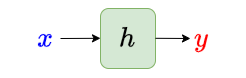
\includegraphics[width=50mm,scale=0.5]{images/regression_images/hypothesis_box.png}
        
            \caption*{Our hypothesis reads an input $x$, and predicts the output $y$.}
        \end{figure}

        \begin{definition}
            A \vocab{hypothesis} is a \gren{function} we use to predict $y$, based on $x$.

            \begin{equation*}
                y = h(x)
            \end{equation*}

            This is also called a \purp{model} in machine learning.
        \end{definition}

        There are many models we could use: this makes it hard to search for a good one.

        \begin{itemize}
            \item One solution is to restrict ourselves to only a certain \orgg{class} of model. 

            Each of these is a different kind of model we could try:

            \begin{equation*}
                h_A(x) = \red{\theta_1} x + \red{\theta_0} 
                \qquad \qquad
                h_B(x) = \blu{\theta_2} x^2 + \blu{\theta_1} x + \blu{\theta_0} 
                \qquad \qquad
                h_C(x) = \grn{\theta_2} \sin (\grn{\theta_1} x) + \grn{\theta_0}
            \end{equation*}
        \end{itemize}

        Each of these formats represents a \purp{hypothesis class}, or a "model class".\\

        \begin{definition}
            A \vocab{hypothesis class} $\mathcal{H}$ is a \purp{set} of possible hypotheses.

            \begin{itemize}
                \item Typically, we include all of the hypotheses with the \gren{same equation format}.
            \end{itemize}
        \end{definition}

        \miniex Let's consider the hypothesis class, represented by $h_A$:
            \note{Not familiar with set notation? $\mathcal{H}_A$ is:
            
            \phantom{}
            
            "the set of every function that looks like $\red{\theta_1} x + \red{\theta_0}$".}

        \begin{equation}
            \mathcal{H}_A = \setty{h(x) \quad : \quad h(x) = \red{\theta_1} x + \red{\theta_0}  }
        \end{equation}

        Here are a few example functions from $\mathcal{H}_A$:

        \begin{equation*}
            \begin{matrix}
                h_1(x) = \red{1}x+\red{5} &&&  h_2(x) = \blu{3}x-\blu{9} &&& h_3(x) = \grn{-10}x+\grn{10} &&& h_4(x) =\org{e^2}x-\org{\pi}
            \end{matrix} 
        \end{equation*}

        This makes things easier: rather than searching all possible hypotheses, we're searching $\mathcal{H}$.\\

        \begin{concept}
            Our goal is to \purp{search} $\mathcal{H}$, to find a good \gren{hypothesis} $h$.
        \end{concept}

        Within a hypothesis class, every hypothesis has the \gren{same structure}.

        \begin{itemize}
            \item What makes a hypothesis different? The \orgg{constants} $\theta_i$.

            \item We call these \vocab{parameters.}\\
        \end{itemize}

        \begin{definition}
            A \vocab{parameter} $\theta_i$ is a \gren{number} that is plugged into the hypothesis.

            \begin{itemize}
                \item Each \purp{hypothesis} $h \in \mathcal{H}$ has a \purp{unique list of parameters} $\Theta$.
            \end{itemize}
        \end{definition}

            \note{Typically, $\theta_i$ is a real number, for our purposes.}

        If we know our model class $\mathcal{H}$, $\Theta$ \gren{fully defines} our hypothesis $h$.

        \begin{figure}[H]
        \centering
            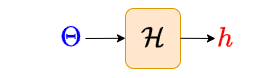
\includegraphics[width=50mm,scale=0.5]{images/regression_images/hypothesis_class.png}
        
            \caption*{By plugging in our $\Theta$ values into the formula for $h$, we get a particular hypothesis.}
        \end{figure}

        For example:

        \begin{figure}[H]
        \centering
            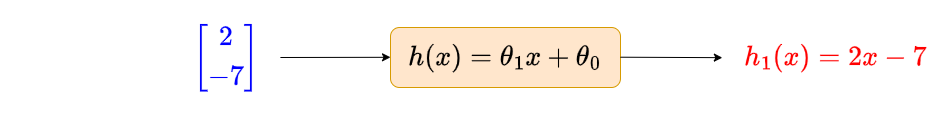
\includegraphics[width=150mm,scale=0.5]{images/regression_images/hypothesis_class_ex.png}
    
        \end{figure}

        This $\Theta$ is what we'll modify, and use to find a \textbf{better model}.\\
        
        \begin{concept}
            Often, we already know which hypothesis class $\mathcal{H}$ we're using.

            \begin{itemize}
                \item So, it's very easy to convert back-and-forth between $\Theta$ and $h$.
            \end{itemize}

            So, we often consider the \purp{parameters} and \gren{hypothesis} interchangeable, or equivalent.

            \begin{itemize}
                \item "Finding a good hypothesis" and "finding good parameters" are, more or less, the same problem.
            \end{itemize}
        \end{concept}

        Notice that we have \orgg{two separate steps} of plugging in, when we use a model $h$:

        \begin{itemize}
            \item When choosing our model $h$, we "plug in" \gren{parameters} $\Theta$ to create our equation.

            \begin{equation}
                h(x) = \grn{\theta_1}x + \grn{\theta_0} 
                \quad \xlongrightarrow{\Theta = \blu{\begin{bmatrix}
                    2 \\ -7
                \end{bmatrix}}} \quad
                h_1(x) = \grn{2}x-\grn{7}
            \end{equation}

            \item When we want to use our model to predict $y$, we "plug in" our \purp{input value} $x$.

            \begin{equation}
                h_1(x) = 2\pur{x}-7 
                \quad \xlongrightarrow{\blu{x=5}} \quad
                h_1(5) = 2(\pur{10})-7 \;\;=13
            \end{equation}
        \end{itemize}

        We'll introduce some new notation to keep the difference clear.\\

        
        
        \begin{notation}
            We can write the same hypothesis $h$ \vocab{two different ways}:

            \begin{equation*}
                h(\red{x}) \qquad \qquad h(\red{x};\blu{\Theta})
            \end{equation*}

            \begin{itemize}
                \item The first notation is denser and \gren{simpler} to read.
                
                \item The second notation includes \purp{$\Theta$}, acknowledging that we had to "plug in" \purp{parameters} to create $h$.
            \end{itemize}

            We \gren{distinguish} between "input variables" and "parameters" by separating them with a \orgg{semicolon} $;$.
        \end{notation}
        
        
        

    \pagebreak
        
    \subsection{The Problem of Regression}
    
        Our hypothesis is a function that solves a \orgg{problem}. What kind of problem are we dealing with?

        We distinguish different types of problems based on two things: 

        \begin{itemize}
            \item \purp{Inputs}: what kind of data do we have to work with?

            \item \gren{Outputs}: what are we trying to predict?
        \end{itemize}

        The notation for functions reflects this idea: what matters most is, "what comes in, and what goes out".
            \note{Functions, of course, weren't specifically designed for machine learning. But the same idea applies to other STEM disciplines.}\\
        
        \begin{notation}
            A \vocab{function} is notated based on what sorts of \gren{inputs} it can take, and the \purp{outputs} it can return. 
            
            A function $f$ is written like this:
            
            \begin{equation*}
                f: \text{set of inputs} \rightarrow \text{set of outputs}
            \end{equation*}
        \end{notation}

        \begin{itemize}
            \item \miniex Suppose that the input is "\orgg{income}" (real number $r \in \RR$) and the output is "\gren{number of hats owned}" (natural number $n \in \NN$). The function for this would be

            \begin{equation*}
                f: \org{\RR} \to \grn{\NN}
            \end{equation*}
        \end{itemize}

        Sometimes, we'll call our set of inputs, the \purp{input space}.\\

        \begin{definition}
            The \vocab{input space} is the set of all \gren{possible inputs} to our hypothesis $h$.
        \end{definition}

            \note{Technically, a \textbf{space} is a set "with \textbf{added} structure", which is about as broad as it sounds.}

        With that out of the way, let's talk about \vocab{regression}:

        \begin{itemize}
            \item In regression, we receive data as a \gren{real-valued vector}, and converting it into a \purp{real number}. 
                \note{Remember the notation for real-numbered vectors we introduced in the last chapter!}
        \end{itemize}
        
        
        Writing this a little more formally:\\
        
        \begin{definition}
            \vocab{Regression} is a \orgg{machine learning problem} where we use a \gren{vector of real numbers} to predict a \purp{real-valued number}.
            
            In other words, we want a \redd{hypothesis} $h$ of the form:
            
            \begin{equation*}
                h: \grn{\RR^d} \rightarrow \pur{\RR}
            \end{equation*}
            
        \end{definition}
        
        \miniex If you have \textbf{3 values} in your input vector (height, weight, age) and \textbf{1 real output} (life expectancy), you would need a hypothesis
        
        \begin{equation*}
            h: \RR^3 \rightarrow \RR
        \end{equation*}
        
        A more visual example:
        
        \begin{figure}[H]
        \centering
            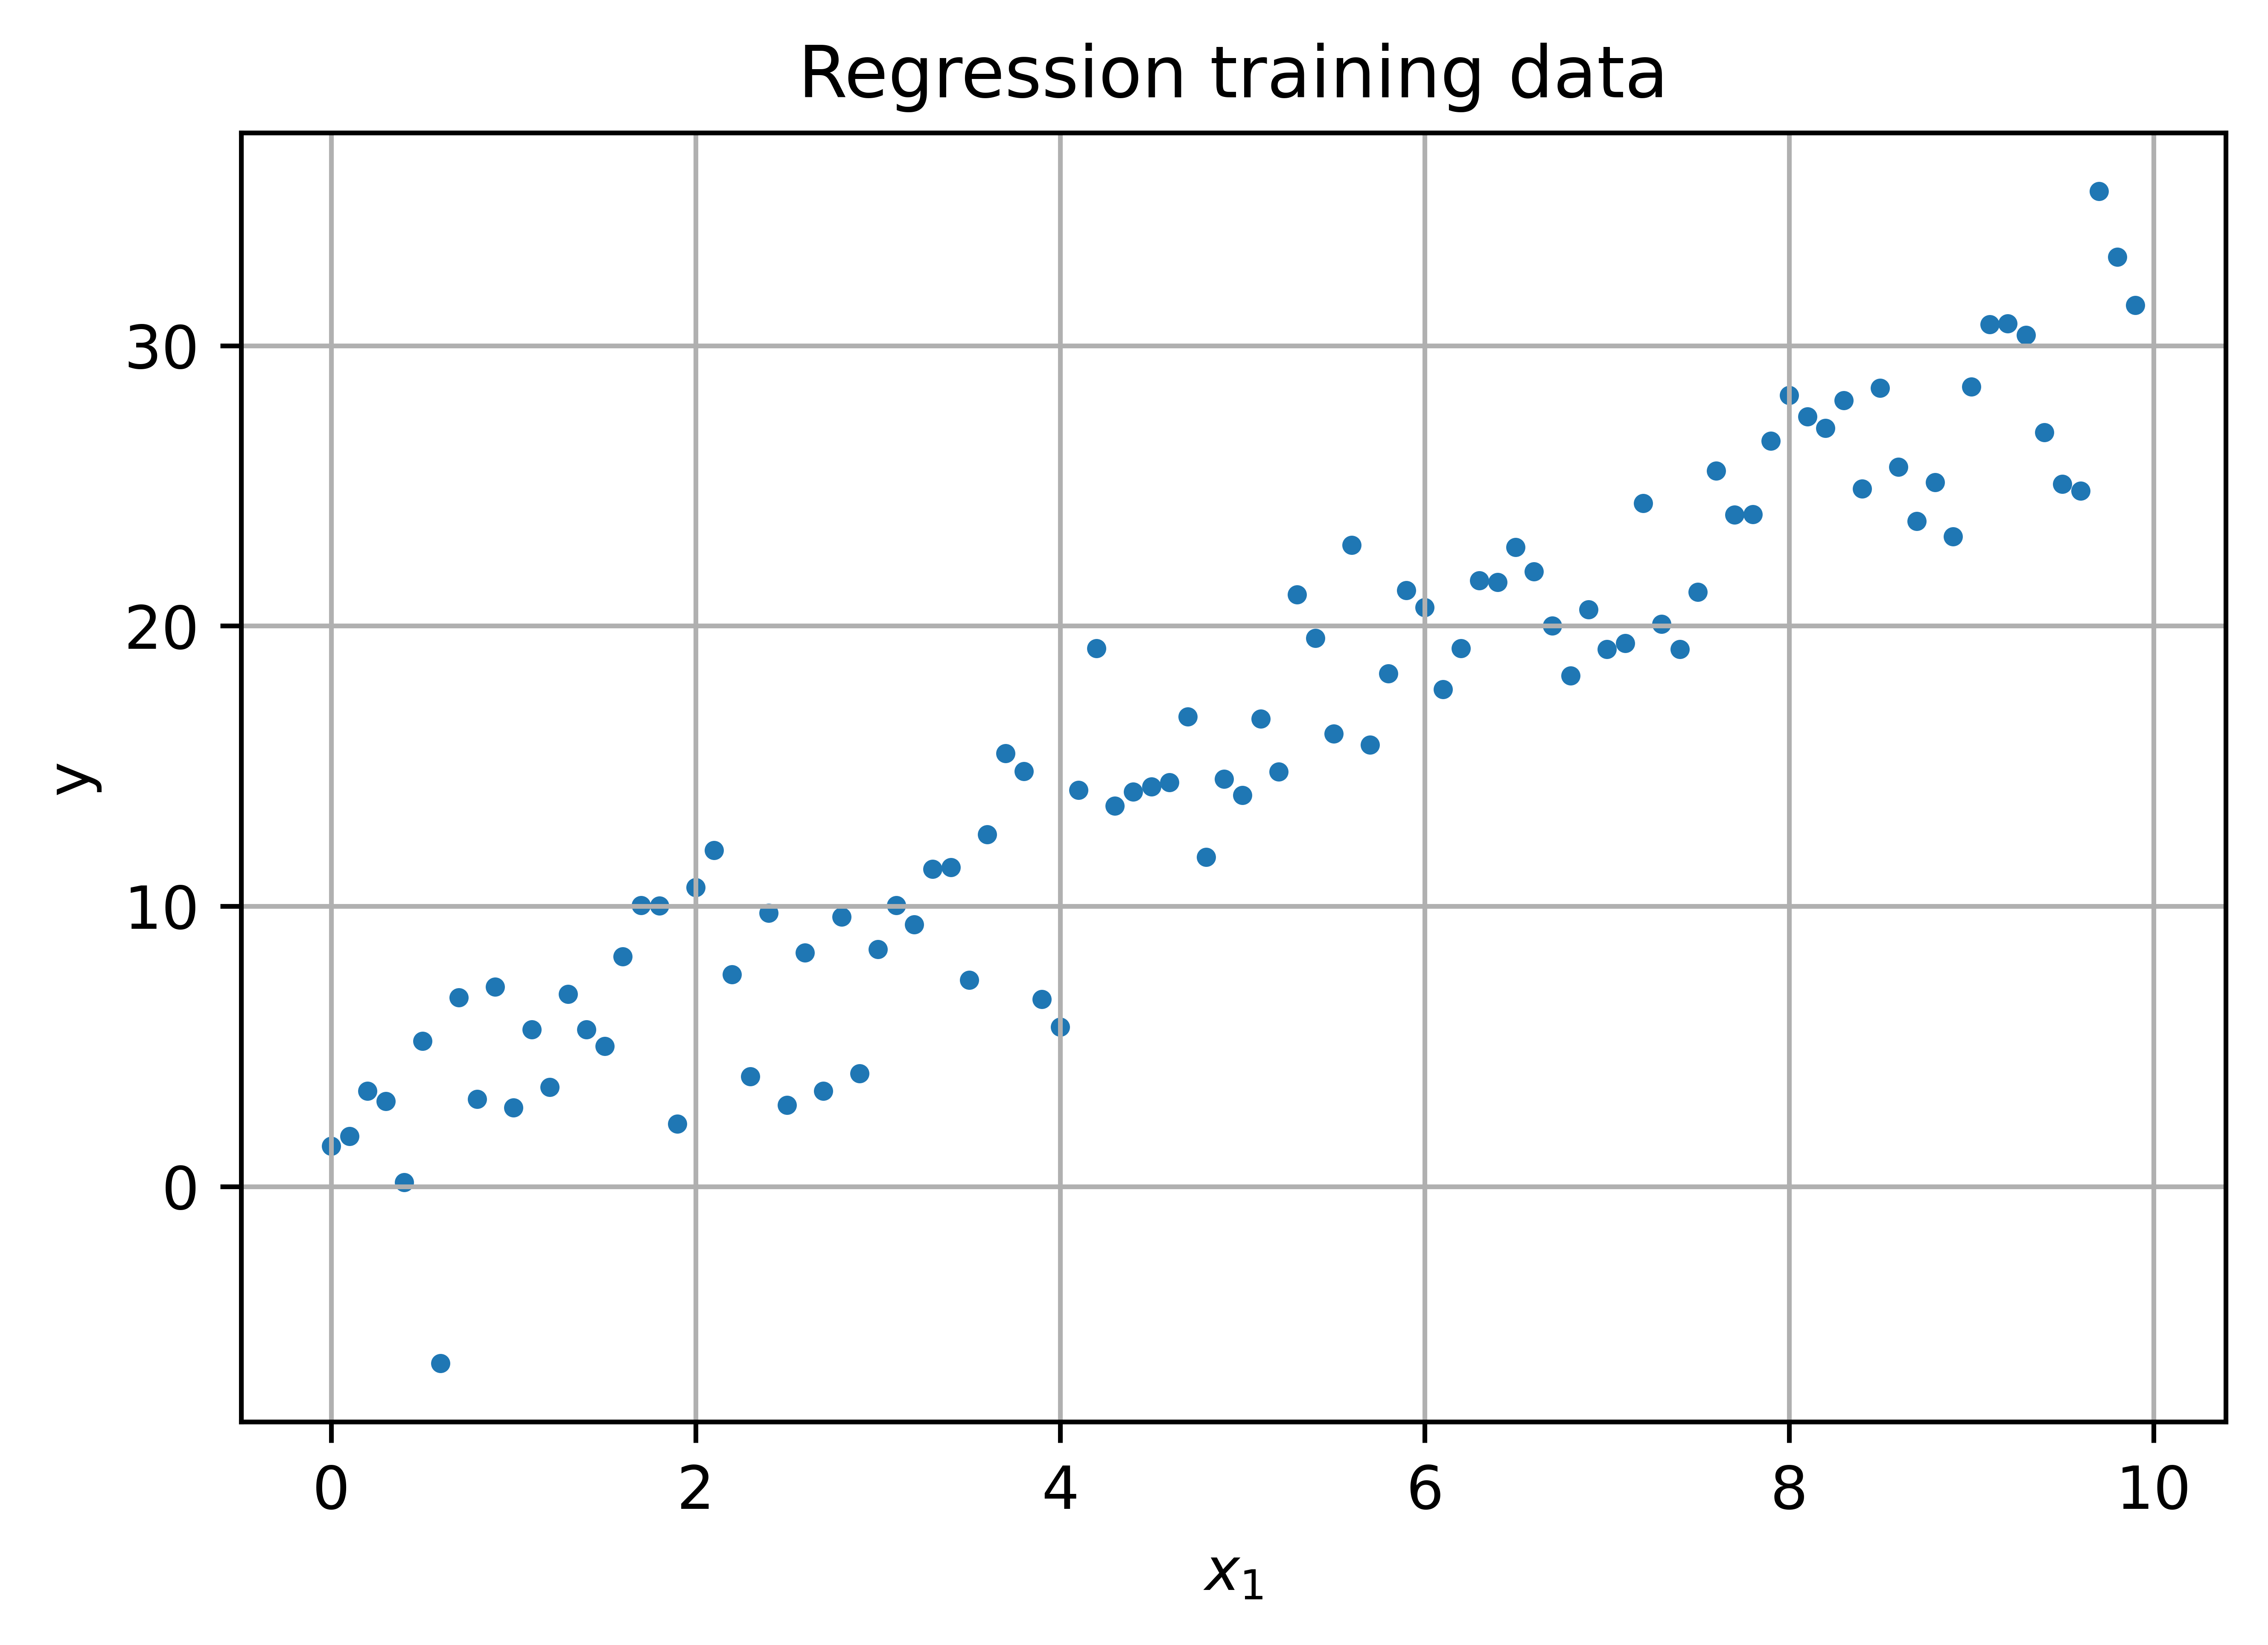
\includegraphics[width=70mm,scale=0.5]{images/regression_images/Regression_Training_Data.png}
        
            \caption*{In this example, you have one input $x \in \RR$ (x-axis), and you want to \textbf{predict} the output $y \in \RR$ (y-axis) based on that. These points are the dataset you want to \textbf{learn} to match.}
        \end{figure}



    \phantom{}
        
    \subsection{Converting our data}
    
        Often, our data \purp{wont fit} this format: maybe we have a car brand, or a color as a variable.

        \begin{itemize}
            \item This requires \gren{converting} this data into real numbers. We do this using something called a \vocab{feature} transformation.\\
        \end{itemize}
        
        
        
        \begin{definition}
            A \vocab{feature} is one distinct piece of \gren{information} in our input.

            \phantom{}
            
            A \vocab{feature transformation} takes those pieces of information, and \purp{transforms} them - often, a more \gren{useful} data type.

            \begin{itemize}
                \item In other cases, we use it on data that's already in the right format, to find \purp{new patterns} in data (we'll return to this idea in a later chapter).
            \end{itemize}
            
        \end{definition}
        
        \miniex You have three car brands. Instead of representing them normally, you instead turn them into vectors: 
        
        \begin{equation}
            \text{Brand A } \to
            \begin{bmatrix}
              1 \\ 0 \\ 0
            \end{bmatrix},
            \;\;\;\;
            \text{Brand B } \to
            \begin{bmatrix}
              0 \\ 1 \\ 0
            \end{bmatrix},
            \;\;\;\;
            \text{Brand C } \to
            \begin{bmatrix}
              0 \\ 0 \\ 1
            \end{bmatrix}
        \end{equation}
        \note{This particular feature transformation is called \textbf{one-hot encoding}! We'll return to it later.}
        
        We do our feature transformation with a function: we often notate this function as $\varphi(x)$.\\

        \begin{notation}
            The \purp{function} we use to do a \vocab{feature transformation} is typically written as $\varphi$.

            \begin{itemize}
                \item If our input data is $x$, the \gren{transformed} data is written as $\varphi(x)$.
            \end{itemize}
        \end{notation}

        \miniex For our above car brand example:

        \begin{equation}
            \varphi\Big(\text{Brand A}\Big) = \begin{bmatrix}
                1 \\ 0 \\ 0
            \end{bmatrix}
        \end{equation}

        There are many different feature transformations for different needs. We will come back to this in a later chapter. 

        \begin{itemize}
            \item For now, we will simply assume that all of our inputs $x$ are \gren{already} in $\RR^d$ (vectors of real numbers).
        \end{itemize}


    \pagebreak
        
        
        
    \subsection{Our dataset}

        Now, we want to find a hypothesis that solves our \textit{particular} regression problem well.

        \begin{itemize}
            \item But in order to predict results, we need \gren{data}.\\
        \end{itemize}

        \begin{concept}
            \vocab{Regression} is a \orgg{supervised problem}:

            This means that, when we're trying to predict the correct answer $y$, we \gren{already have} that answer.

            \begin{itemize}
                \item That way, we can check how good/bad our model's \purp{prediction} was.
            \end{itemize}
        \end{concept}

        \miniex A student practicing "supervised learning" has a practice exam, with all of the solutions.

        \begin{itemize}
            \item They try to do the exam \orgg{without} looking at the solutions.
            \item After they finish, they \gren{check} the solutions, to see what they did wrong, and how they can do better.
        \end{itemize}

        In this analogy, each data point includes a "\gren{question}" (input $x$) and the "\purp{answer}" (output $y$) to that question.

        \begin{figure}[H]
            \centering
            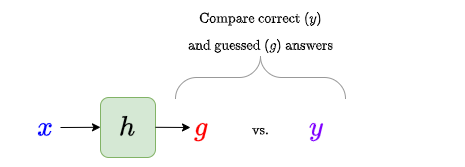
\includegraphics[width=90mm,scale=0.5]{images/regression_images/hypothesis_guess.png}
        
            \caption*{Our model doesn't actually produces $y$: it produces a guess $g$, which we hope is similar to $y$.}
        \end{figure}
        
        We want to \orgg{pair up} inputs with their correct outputs, so we'll write our first data point as 

        \begin{equation}
            \Big(x,y \Big)
        \end{equation}

        But we have many data points we need to sort, like this.

        \begin{itemize}
            \item We'll distinguish each data point using $\ex{x}{i}$ notation, from last chapter:\\
        \end{itemize}

        \begin{notation}
            $x^{(i)}$ is the \vocab{$\nth{i}$ data point}, represented as a vector.

            \begin{itemize}
                \item Sometimes, you may instead see the notation $x_i$.
            \end{itemize}
            
        \end{notation}
        
        We can rewrite this as:
        
        \begin{equation*}
            \left( \ex{x}{1}, \ex{y}{1} \right)
        \end{equation*}
        
        Repeating this for all of our data, we have a set of $n$ data points, $\dataTrain$:
        
        \begin{equation*}
            \dataTrain = 
            \left\{  
            \left(\ex{x}{1}, \ex{y}{1}\right), \dots,
            \left(\ex{x}{n}, \ex{y}{n}\right)
            \right\}
        \end{equation*}

    \phantom{}
        
    \subsection{Training our model}

        We'll use this \purp{training data} to train our model: hopefully, if our model performs well with this limited data, it'll perform well with new data.
            \note{But as we'll see below, that's not always the case.}

        In order to train our model, we need to know how \gren{good} or bad it is, on the data we can see.

        \begin{itemize}
            \item We'll measure the "badness" of our model as \vocab{loss}, from last chapter.\\
        \end{itemize}

        

        \begin{definition}
            \textit{(Review from Introduction Chapter)}
        
            A \vocab{loss function}  measures how \purp{poorly} your machine is \purp{performing} on a \gren{task}.

            \begin{itemize}
                \item The output is a \gren{real number}.
            \end{itemize}
        \end{definition}
        
            \note{If your machine is performing \purp{well}, then you will have a \purp{low} output. And vice versa: if it is doing \gren{badly}, it will have a \gren{high} output.}

        \begin{figure}[H]
            \centering
            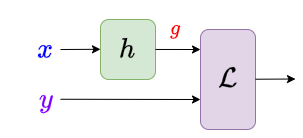
\includegraphics[width=70mm,scale=0.5]{images/regression_images/hypothesis_loss.png}
            \caption*{Our loss function gives us our tool for "comparing" $y$ to $g$.}
        \end{figure}

        We'll take the \purp{average} loss, across all of our \purp{training data}. This is our \vocab{training error}.\\

        \begin{kequation}
        
            \vocab{Training Error} $\trainerr$ is written as:
            
                \begin{equation*}
                    \trainerr(h) \;=\; \red{ \frac{1}{n}  \sum_{i=1}^n } \ex{Loss}{i} \quad=\quad 
                    \frac{1}{n}  \sum_{i=1}^n \loss 
                    \left( \pur{ h(\ex{x}{i}), \; \ex{y}{i} } \right)
                \end{equation*}

            This is the \orgg{expected} (average) loss over all of our training data.
        \end{kequation}

        Note that this is a bit weird: we're using $h$ as an input.

        \begin{itemize}
            \item We want $\trainerr$ to \gren{evaluate} and compare different hypotheses $h$: it has to receive that hypothesis in order to evaluate it.
                \note{The hypothesis, in turn, takes the training data as input.}\\
        \end{itemize}

        \begin{clarification}
            $\vocab{h}$ is a \gren{function} that takes a \gren{variable}, $x$, as its input. This is the usual format.
            
            \vocab{$\trainerr$} is also a function, but it takes in $h$, a \orgg{different function}, as an input!

            \begin{itemize}
                \item That means one function is using \purp{another function} as an input. This can sometimes cause confusion.
            \end{itemize}

            We do this because $\trainerr$ observes our hypothesis, and outputs, "\purp{how bad} in this particular hypothesis at \gren{predicting} this data".
        \end{clarification}

        "Training", in the simplest case, boils down to reducing our error as much as possible.
            \note{Below, we'll add another component, that makes this more complicated.}

            \begin{itemize}
                \item But wait: our goal \purp{isn't} to improve performance on our \gren{training data}. 

                \item Our goal is to perform well on \orgg{new data}!
            \end{itemize}

    \phantom{}
        
    \subsection{Learning to Generalize}
            
        Above, our idea was, "get better at practice data, get better at future data". But this has a problem:

        \begin{itemize}
            \item Even though our training data and future data should be from the \gren{same distribution} (IID), \orgg{randomness} means they won't be exactly the same.
                \note{So if we perfectly matched our training data, we'd be inaccurate to the real distribution.}
        \end{itemize}

        In the last chapter, we introduced a solution: a second dataset, that we \purp{test} our data on.

        \begin{itemize}
            \item We want our machine to handle \gren{new situations} it hasn't seen before: testing data allows us to try out a "new situation".\\
        \end{itemize}

        \begin{definition}
            \vocab{Generalization} is the ability to take something \purp{specific}, and apply it to something more \gren{broad}.

            \begin{itemize}
                \item In machine learning, we want our model to look at some \purp{limited data}, and be able to perform well on a much larger body of \gren{future data} it hasn't seen before.
            \end{itemize}
        \end{definition}
        
        So, let's find out how well our model generalizes. We'll define \vocab{test error}: our performance on the \purp{testing data}. This time, we have $m$ new data points.
        
        \begin{equation}
            \testerr(h) = \frac{1}{\red{m}}  \sum_i  \loss 
            \left( h(\ex{x}{i}), \; \ex{y}{i} \right) 
        \end{equation}
        
        We'll start counting from $n+1$ because we've already used the first $n$ points when training.
            \note{We could start over from $i=1$, but that would be a bit confusing. If you said "the 10th data point", someone might ask, "from the training, or testing data? This avoids this problem.}
        
        \begin{kequation}
        
            \vocab{Testing Error} $\testerr$ is written as:
            
            \begin{equation*}
                \testerr(h) =
                \frac{1}{m}  \sum_{i\purp{=n+1}}^{\purp{n+m}} \loss 
                \left( h(\ex{x}{i}), \; \ex{y}{i} \right) 
            \end{equation*}
        \end{kequation}
        
        
        Because we want to generalize, we want to minimize \textbf{test error}.
        
        \begin{itemize}
            \item But, because we want our model to do well on "data it \gren{hasn't seen} before", we can't use it during our training process.
        \end{itemize}
        
        For now, the next best thing after "minimize test error" is "\vocab{minimize training error}", while using techniques to improve how we \orgg{generalize}. 
            \note{How can we "generalize" if we can't see all of that extra data? We'll get into that below.}

\pagebreak
%%%%%%%%%%%%%%%%%%%%%%%%%%%%%%%%%%%%%%%%%%%%%%%%%%%%%%%%%%%%%%%%%%%%%%%%%%%%%%%%%%%%%%%%%%%

\section{Regression as an optimization problem}
    
    We want to make our \purp{loss} (error) as low as we can: we want to \gren{minimize} it. This is a form of \vocab{optimization} - getting the best results from our system.
        \note{Most of computer science boils down to some kind of optimization.}
    
    Here, we'll introduce some of the terms and notation of optimization.

    \phantom{}
    
    \subsection{Objective Function}

        Now, we confront a major challenge: we have two different priorities.

        \begin{itemize}
            \item We want to perform well on \purp{training data}: our model will learn some insights about the true distribution of data.

            \item But we also want our model to \orgg{generalize} well: we want it to do well data on it has never seen before.
                \note{Because our training data gives us a limited view of the true distribution.}
        \end{itemize}

        Currently, our approach focuses on one priority: we measure our success using \gren{training error}.

        \begin{equation}
            \frac{1}{n}  \sum_{i=1}^n \loss 
                    \left( \pur{ h(\ex{x}{i}), \; \ex{y}{i} } \right)
        \end{equation}

        \begin{itemize}
            \item This function represents "what we consider \gren{important}": it mathematically describes what we want to improve.

            \item We call this an \vocab{objective function}.\\
        \end{itemize}

        \begin{definition}
            An \vocab{objective function} $J$ is the function that tells us what we want to improve, or \purp{optimize}:
            
            \begin{itemize}
                \item Usually, this means that our goal is \gren{minimizing} it.
            \end{itemize}
            
            We minimize our objective function by adjusting our model, via \orgg{parameters} $\Theta$. So, we take that as our input: \purp{J($\Theta$)}.
        \end{definition}

        Since we are focusing more on $\Theta$ then before, we'll replace $h(\ex{x}{i})$ with \blu{$h(\ex{x}{i}; \Theta)$}:
        
        \begin{equation*}
            J(\Theta) = \text{Training Error} = 
            \frac{1}{n}  \sum_{i=1}^n \loss \Big( h(\ex{x}{i}; \blu{\Theta}), \ex{y}{i} \Big) 
        \end{equation*}

    \subsection{The Regularizer}

        If our objective function describes "what we care about", and we care about \gren{generalization}, shouldn't we \purp{include} it in our objective function?

        \begin{itemize}
            \item Let's do that: we'll call it a \redd{regularizer} term.
        \end{itemize}

        \begin{equation}
            J(\Theta) = \text{Training Error} + \red{\text{Regularizer}}
        \end{equation}

        We continue using our training error from before:

        \begin{equation}
            J(\Theta) = \frac{1}{n}  \sum_{i=1}^n \loss 
                    \left( \pur{ h(\ex{x}{i}; \Theta), \; \ex{y}{i} } \right) + \red{\text{Regularizer}}
        \end{equation}

        Later, we'll construct our regularizer so that minimizing it will create a \gren{more general} model $\Theta$. 

        \begin{itemize}
            \item Because we want to make $\Theta$ more \gren{general}, we'll use it in our regularizer: we'll call it \red{$R(\Theta)$}.
                \note{Our strategy is to \gren{minimize} $J(\Theta)$: by reducing training loss and $R(\Theta)$, we hope to make a better model.}
        \end{itemize}

        \begin{equation}
            J(\Theta) = \frac{1}{n}  \sum_{i=1}^n \loss 
                    \left( \pur{ h(\ex{x}{i}; \Theta), \; \ex{y}{i} } \right) + \red{R(\Theta)}
        \end{equation}

        We're missing one thing: how much do we want to prioritize \red{$R(\Theta)$}, compared to \purp{training error}?

        \begin{itemize}
            \item We'll \vocab{scale} our regularizer by a \gren{constant} $\lambda \geq 0$.

            \item The larger $\lambda$ is, the more we care about \orgg{generalizing} to new data.\\
        \end{itemize}

        \begin{kequation}
            
            In general, we write the \vocab{objective function} as:
            
            \begin{equation*}
                J(\Theta) =
                \left( 
                \frac{1}{n}  \sum_{i=1}^n \loss \Big( h(\ex{x}{i}; \Theta), \;\; \ex{y}{i} \Big) 
                \right)
                +
                \blu{\lambda} \red{ R(\Theta)}
            \end{equation*}

            \begin{itemize}
                \item The left term is the \purp{loss}: how well we perform on training data.
                \item The right term is the \orgg{regularization}: we hope that \gren{minimizing} it will make our model more "general" (good for new situations).
            \end{itemize}
        \end{kequation}

        This is the function we want to \gren{minimize}. What does our \redd{regularizer} look like? 

        

        \begin{itemize}
            \item We'll come back to this later. we'll go one step at a time, and first learn how to minimize \purp{training error}.
        \end{itemize}

    \subsection{More on the Objective Function}

        Notice that our objective function \gren{depends} on our training data $\data$ as well: the same model will work better for some problems, than others.
    
        \begin{itemize}
            \item \miniex A model trained in political science learns different things compared to one trained in geology.
            \item We'd expect it to perform pretty badly on a geology exam.
        \end{itemize}
    
        "$\data$ affects $J$, but isn't the main input" is \gren{similar} to our previous idea: "$\Theta$ affects hypothesis $h$, but we usually \purp{don't} think of it as the \purp{input}".
        
        \begin{itemize}
            \item We made this distinction with some \orgg{notation}: $h(x;\Theta)$.\\
        \end{itemize}
    
        \begin{notation}
            Just like how we can use ";" when writing $h(x;\Theta)$, we'll use the \orgg{same notation} for $J$: $J(\Theta;\grn{\data})$
    
            \begin{equation*}
                    J(\Theta; \grn{\data}) =
                    \left( 
                    \frac{1}{n}  \sum_{i=1}^n \loss \Big( h(\ex{x}{i}; \Theta), \;\; \ex{y}{i} \Big) 
                    \right)
                    +
                    \blu{\lambda} \red{ R(\Theta)}
                \end{equation*}
    
            $\Theta$ is our "main" input variable, but data $\data$ is important for computing $J$.
        \end{notation}

        One more comment:\\

        \begin{clarification}
           Students often get confused by the fact that our \purp{objective function} $J$ is a function of $\Theta$, while \orgg{training error} $\trainerr$ is a function of $h$.

           \begin{equation*}
               \overbrace{
                    J(\Theta)}^{\text{Uses } \Theta} 
                =
                \overbrace{
                    \trainerr(h)}^{\text{Uses } h} 
                + \lambda R(\Theta)
           \end{equation*}
            
            The difference is that \orgg{training error} $\trainerr(h)$ is \gren{more general} than the \purp{objective function} $J(\Theta)$, and \orgg{$h$} is \gren{more general} than \purp{$\Theta$}.

            \begin{itemize}
                \item By "more general", we mean that there are more situations where we can use $h$ than $\Theta$.
                \begin{itemize}
                    \item $\Theta$ is a list of parameters: we only use it if we have a \purp{parametric model}.
                    \item $h$ is used if we have \orgg{any kind of model}.
                \end{itemize}
            \end{itemize}

            
            So, let's compare $\trainerr(h)$ and $J(\Theta)$:
            
            \begin{itemize}
                \item \orgg{Training error} 
                can be used for any model $h$, so we don't want to use $\Theta$: our model could be \gren{non-parametric}.
                
                \item Our \purp{objective function} \gren{assumes} we have parameters $\Theta$: we know our model class $H$, we just want to optimize $\Theta$.
            \end{itemize}
            
        \end{clarification}
        
    \pagebreak
        
        
        
        
        
        
    \subsection{Minimization Notation}
        
        Our goal is to \gren{minimize} $J$ by adjusting $\Theta$. To demonstrate, we'll use the following example:

        \begin{figure}[H]
            \centering
            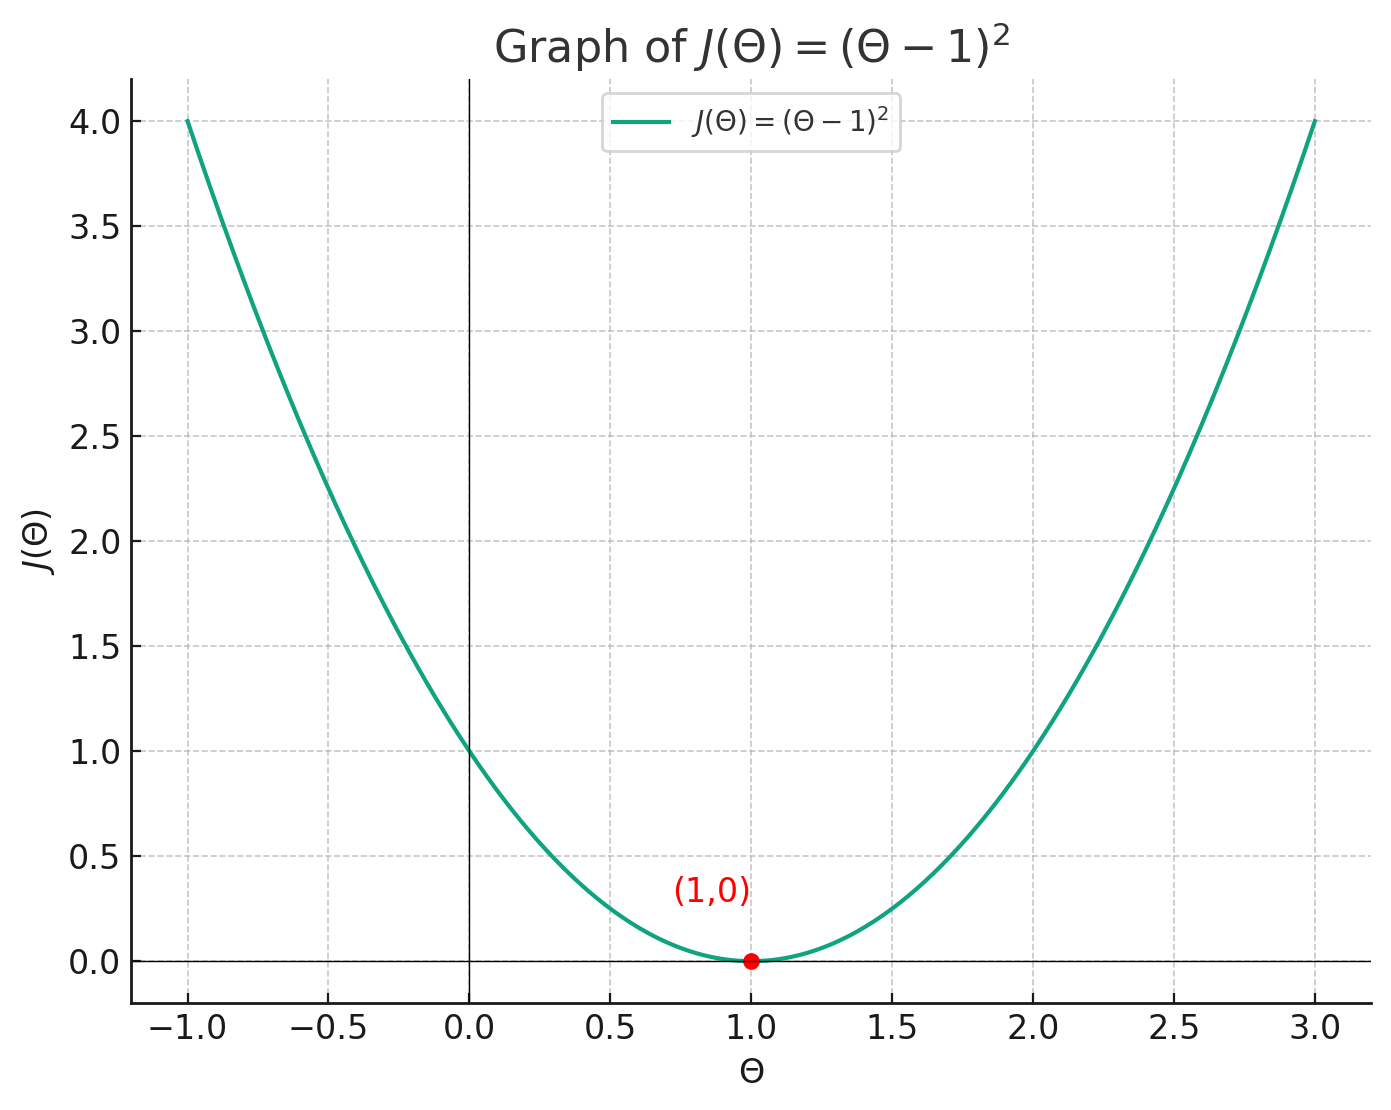
\includegraphics[width=70mm,scale=0.5]{images/regression_images/minimizing_(x-q)^2.png}
        
            \caption*{Take $J(\Theta)=(\Theta-1)^2$. The minimum output is 0, which happens at $\Theta=1$. So, we have a minimum at $(1, 0)$.}
        \end{figure}

        Our goal is to find this \vocab{minima}. There are two questions we're interested in:

        \begin{itemize}
            \item What is the \purp{minimum value of $J$} we can find by \orgg{adjusting $\Theta$}?
            \item Which \gren{model $\Theta$} gives us the minimal $J$? In other words: which model performs best?
        \end{itemize}

        We define a distinct function for answering each of these questions. 
        
        \phantom{}
        
        First:
        
        \begin{itemize}
            \item What is the \purp{minimum value of $J$} we can find by \orgg{adjusting $\Theta$}?\\
        \end{itemize}
        
        \begin{notation}
            The \vocab{min function} gives you the \gren{minimum output} of a function we get by adjusting one chosen \purp{variable}.
            
            \begin{equation*}
                \min_{ \pur{ \Theta } }{ \grn{ J(\Theta) } }
            \end{equation*}
            
            The \gren{function we want to minimize} is written to the right, while the \purp{variable we adjust} is written below.
        
        \end{notation}
        
        \miniex 
        
        \begin{equation}
            \min_{\Theta}{ \red{(\Theta-1)^2} } = \red{0}
        \end{equation}

        0 is the minimum value of $J$ we can find by adjusting $\Theta$.

        \phantom{}

        Next:
        
        \begin{itemize}
            \item What is the \purp{minimum value of $J$} we can find by \orgg{adjusting $\Theta$}?\\
        \end{itemize}
        
        \begin{notation}
            The \vocab{argmin function} tells you the value of the \purp{input variable} that gives the \gren{minimum output}.
            
            \begin{equation*}
                \argmin{ \pur{ \Theta } }{ \grn{ J(\Theta) } }
            \end{equation*}
            
            The \gren{function we want to minimize} is written to the right, while the \purp{variable we adjust} is written below.
        
        \end{notation}
        
        \miniex
        
        \begin{equation}
            \argmin{\red{\Theta}}{ (\Theta-1)^2 } = \red{1}
        \end{equation}

        1 is the value of $\Theta$ which gives the minimum $J$.\\

        \begin{clarification}
            Why is it called "\vocab{argmin}"?

            "\gren{Argument}" is used as another word for "\gren{input variable}".

            And our argmin function returns the \gren{argument} with the \purp{minimum} output. Hence, \gren{arg} \purp{min}.
        \end{clarification}
        
          

        

        \phantom{}
        
    \subsection{Optimal Value Notation}
        
        Our goal is to find the best model, represented by some $\Theta$. We'll call this "optimal" model, $\Theta^*$.\\
        
        \begin{notation}
            We add a \vocab{star} $^*$ to indicate the \purp{optimal} variable choice.
            
            If that variable is $z^*$, you would say it as "$z$-star".
        \end{notation}
        
        \miniex 
        
        \begin{equation}
            \Theta^* = 1 \text{ for the above example.}
        \end{equation}
        
        So, if we want optimal $\Theta$, we're looking for:\\
        
        \begin{kequation}
        
            Our \vocab{optimal parameter} vector is written as 
            
            \begin{equation*}
                \Theta^* = \argmin{ \Theta  }{  J(\Theta)  }
            \end{equation*}
        \end{kequation}
        


\pagebreak
%%%%%%%%%%%%%%%%%%%%%%%%%%%%%%%%%%%%%%%%%%%%%%%%%%%%%%%%%%%%%%%%%%%%%%%%%%%%%%%%%%%%%%%%%%%

\section{Linear Regression}

    Now that we understand the problem of \gren{regression}, and the concept of \purp{optimizing} over it, we'll introduce our \orgg{hypothesis class.}
    
    We want a function that can use information to \gren{predict} outputs.
    
    \subsection{The Linear Model, 1-D}
    
        We'll start off small: we have \gren{one variable}, and something we want to predict. And we'll pick the simplest pattern we can:

        \begin{equation}
            y = mx+b
        \end{equation}
        
        A \vocab{linear} equation.
        
        \begin{itemize}
            \item $m$ tells us \textbf{how much} our input $x$ \gren{affects} our output $y$.
            \item $b$ accounts for everything \purp{unrelated} to $x$: what is $y$ when $x=0$?
        \end{itemize}

        $b$ and $m$ are our \orgg{parameters}: that means they're part of $\Theta$. We'll rename them $b=\theta_0$ and $m=\theta_1$.\\
        
        \begin{equation}
            h(x) = \red{\theta_1} x + \blu{\theta_0}
        \end{equation}

        \begin{figure}[H]
            \centering
            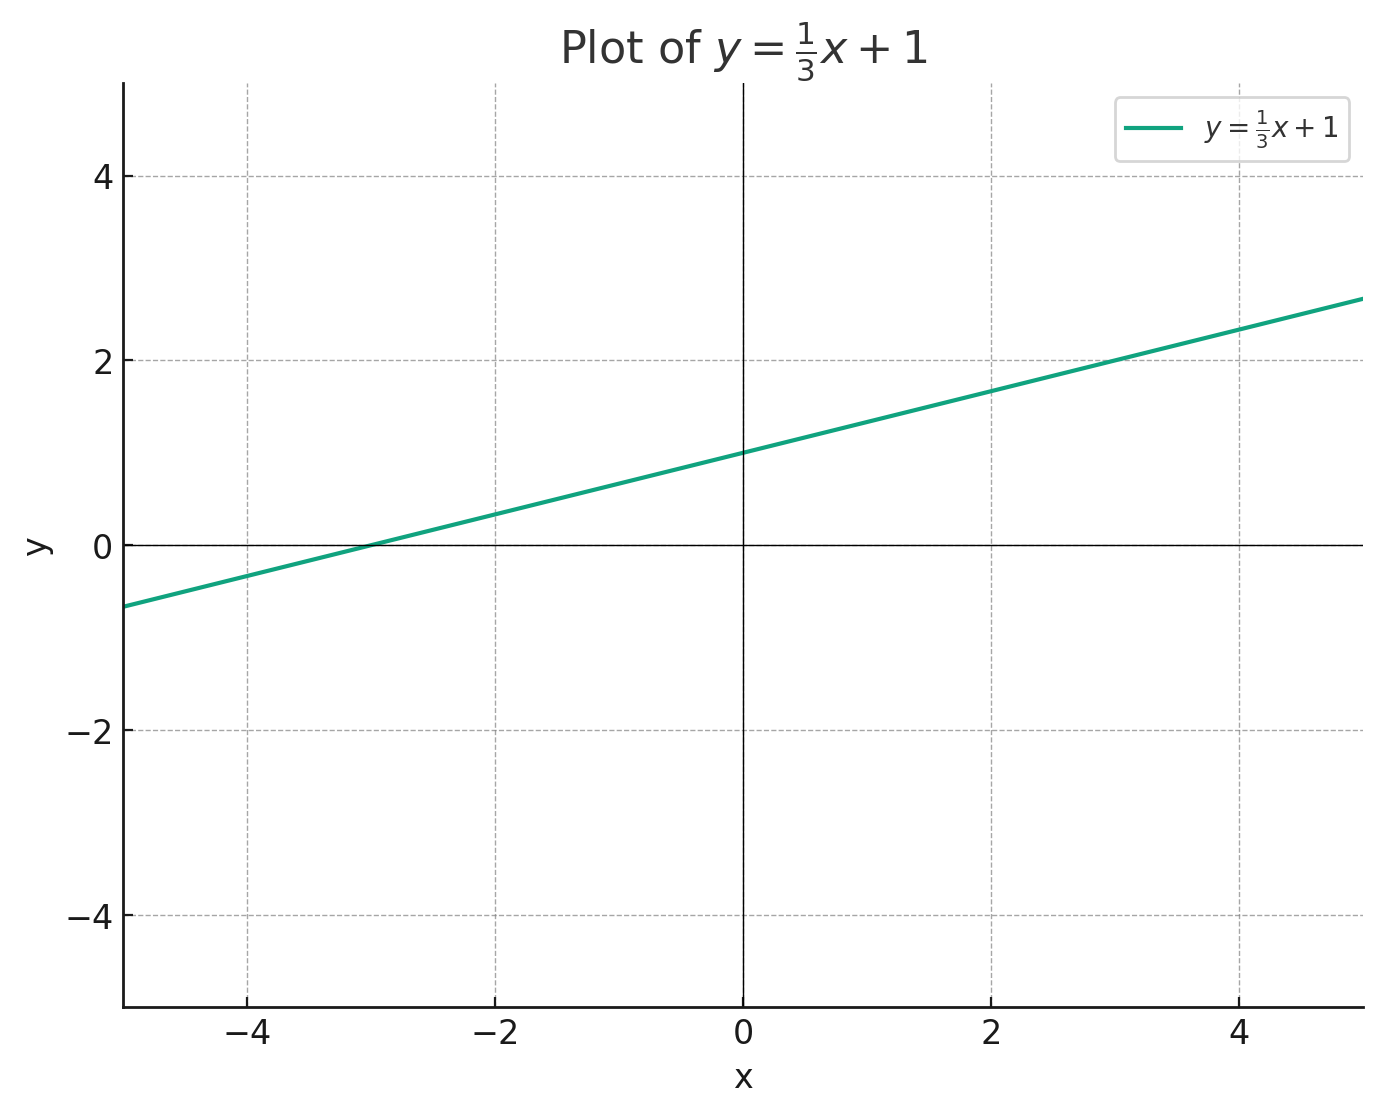
\includegraphics[width=50mm,scale=0.5]{images/regression_images/xover3+1.png}
        
            \caption*{Here's $\frac{1}{3}x+1$. We call this 1D because there's only one input dimension, $x$. But we plot it in 2D to see the output, too!}
        \end{figure}

    \phantom{}
        
    \subsection{The Linear Model, 2-D}
    
        We want to have \textbf{multiple} input variables: $x$ will be a \purp{vector}, not a number. 

        \begin{equation}
            x = \begin{bmatrix}
                x_1 \\ x_2
            \end{bmatrix}
        \end{equation}
        
        So, for our above example, we'll \textbf{replace} $x$ with $x_1$.
        
        \begin{equation}
            h(x) = \theta_1 \red{x_1} + \theta_0
        \end{equation}
        
        The simplest way to include $x_2$ by just \textbf{adding} it. We have a scaling factor $\theta_1$ for $x_1$, so we'll give $x_2$ its own \gren{parameter}, $\theta_2$:
        \note{If $\theta_1$ is the "slope" for $x_1$, $\theta_2$ is the "slope" for $x_2$.}
        
        \begin{equation}
            h(x) = \red{\theta_2 x_2} + \theta_1 x_1 + \theta_0
        \end{equation}

        \begin{figure}[H]
            \centering
            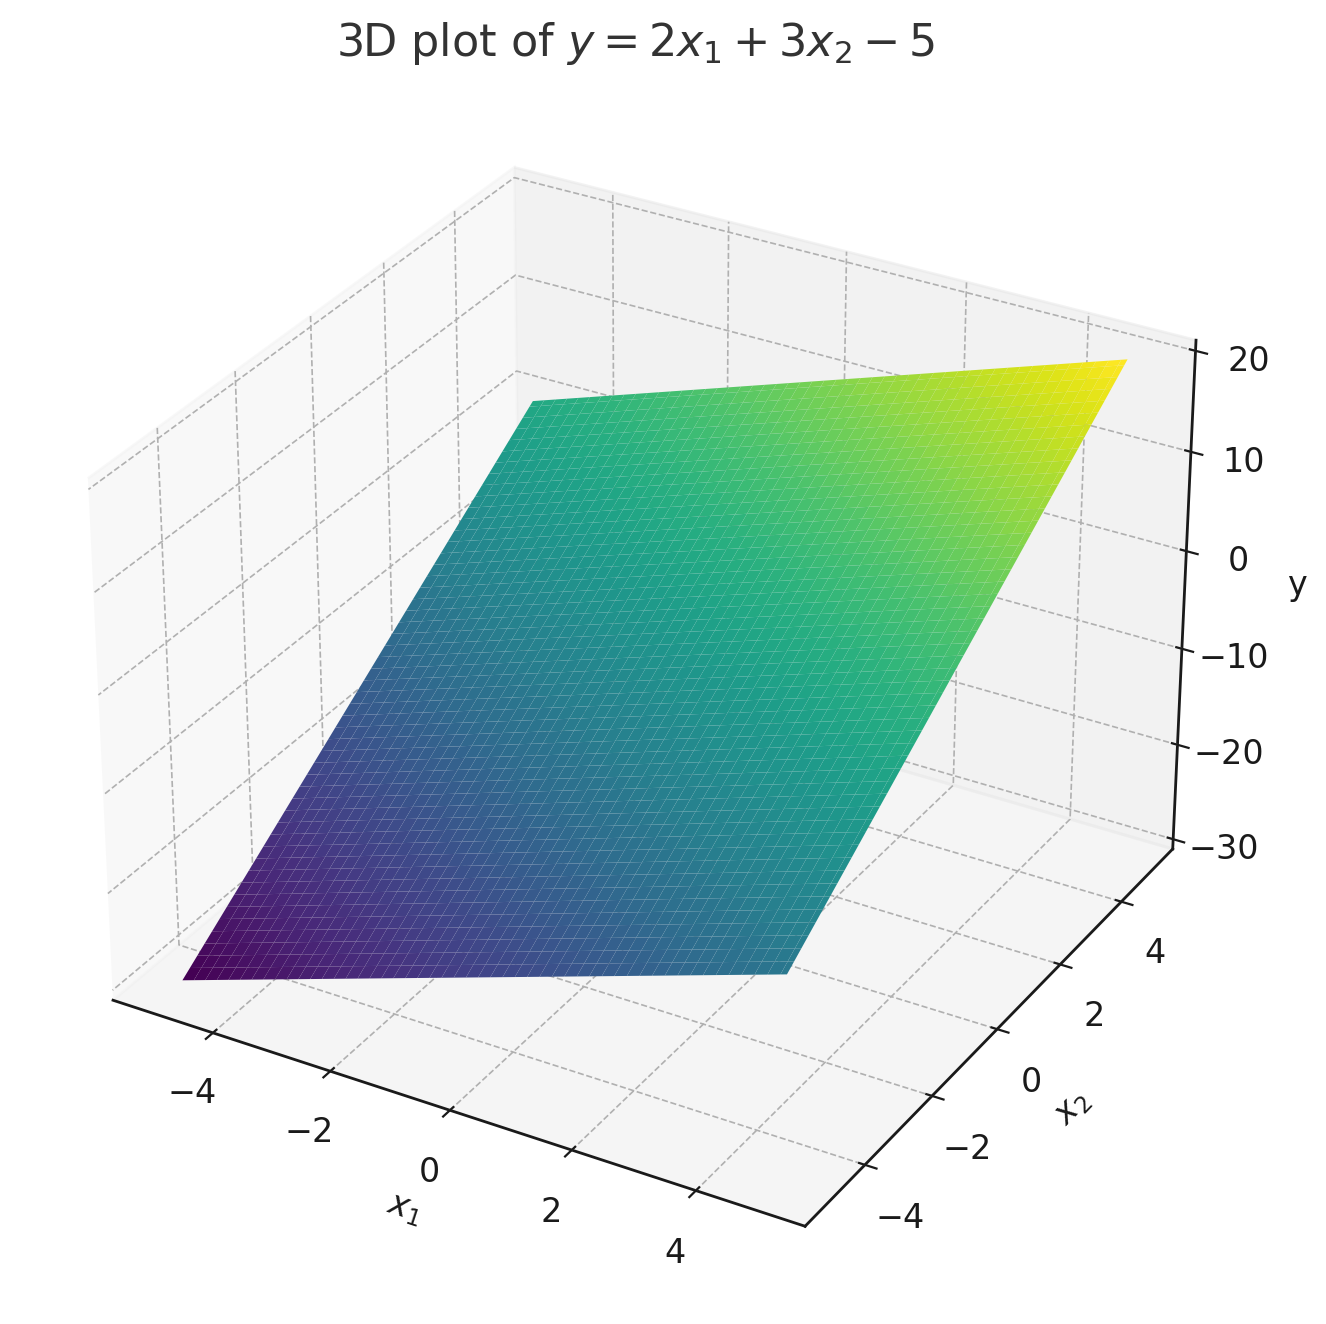
\includegraphics[width=50mm,scale=0.5]{images/regression_images/plane.png}
        
            \caption*{Here's a 2d regression: it's a plane. The height represents the output.}
        \end{figure}
        
    \subsection{The Linear Model, $d$-D}
    
        You can \textbf{expand} this to $d$ dimensions by \purp{adding more terms}:
        \note{This is the "dimension" of our input space: the \textbf{number} of input variables we have.}
        
        \begin{equation}
            h(x) = \blu{\theta_0} + \red{\theta_1}x_1 + \red{\theta_2}x_2 + \red{\theta_3}x_3 + ... + \red{\theta_d}x_d
        \end{equation}

        We need $n+1$ dimensions to plot an $n$-dim regression, so... we can't plot $n>2$.

    \phantom{}
        
    \subsection{The Linear Model using Vectors}
        
        We \textbf{multiply} components of $x$ and $\theta$ together, then \textbf{add} them together. This looks like a \orgg{dot product}:
        
        \begin{equation}
            h(x) = \theta_0 +
            \red{
                \begin{bmatrix}
                    \theta_1 \\ \theta_2 \\ \vdots \\ \theta_d
                \end{bmatrix}
                }
                \cdot
                \blu{
                \begin{bmatrix}
                    x_1 \\ x_2 \\ \vdots \\ x_d
                \end{bmatrix}
            }
        \end{equation}
        
        If we write this symbolically, we get:
        
        \begin{equation}
            h(x) = \theta_0 + \red{\theta} \cdot \blu{x} 
        \end{equation}
        
        $\theta$ includes all of our parameters, \orgg{except for} $\theta_0$.
        
        \begin{itemize}
            \item $\theta$ is used for our \textbf{dot product}, $\Theta$ includes \textbf{all} parameters.\\
        \end{itemize}
        
        \begin{notation}
            We represent the \gren{parameters} of our \purp{linear} equation as $\Theta = (\theta, \theta_0)$.
        \end{notation}
        
        This formula looks similar to $y=mx+b$ again! Only this time, we have \textbf{vectors} instead.
        
        We'll swap out the dot product for \purp{matrix multiplication}.\\

        \begin{kequation}
            A dot product $a \cdot b$ can be written as \vocab{matrix multiplication} instead:

            \begin{equation*}
                a \cdot b = a^Tb
            \end{equation*}
        \end{kequation}
        
        In this class, we'll usually find it more useful to work with matrix multiplication.\\
        
        \begin{definition}
            The \vocab{linear regression} hypothesis is  $h(x)=\theta \cdot x+\theta_0$, or
            
            \begin{equation*}
                h(x) = \red{ \theta^T x } + \theta_0
            \end{equation*}
        \end{definition}
        
        \note{Make sure you know what $\theta^T$ is: it's the \textbf{transpose} of $\theta$.}
        
        Remember that, when written out, this looks like:
        
        \begin{equation}
            h(x) = 
            \red{
                \begin{bmatrix}
                    \theta_1 & \theta_2 & \theta_3 & \cdots & \theta_d
                \end{bmatrix}
            }
            \blu{
                \begin{bmatrix}
                    x_1 \\ x_2 \\ x_3 \\ \vdots \\ x_d
                \end{bmatrix}
            }
            + \theta_0
        \end{equation}
        
        This is the \vocab{hypothesis class} of \textbf{linear hypotheses} we will reuse throughout the class.

    \pagebreak
        
    \subsection{Regression Loss}
    
        We need to decide on our \vocab{loss function} for regression: how \purp{badly} is our model is performing?

        \begin{itemize}
            \item Our goal is for our \purp{guess} $g$ to be close to the \gren{real} output $y$. 

            \item The more \orgg{different} they are, the worse.
        \end{itemize}

        We could use "absolute difference" $|g-y|$, but \vocab{squared difference} tends to be much more useful:
            \note{Why? We discuss in the Concept box below.}
        
        \begin{equation}
            \loss(g,y) = (g-y)^2
        \end{equation}
        
        We call this \vocab{square loss}. It punishes high and low guesses equally, and the punishments become more \textbf{severe} as the \textbf{difference} increases.
        \note{Our slope $\deriv{}{x} x^2 = 2x$ gets larger as we move away from $x=0$.}\\

        \begin{concept}
             We use \vocab{square distance} for a few good reasons:
        
        \begin{itemize}
            \item High and low guesses are treated \purp{equally}.
            
            \item It works well with \orgg{matrix multiplication}:

                \begin{equation*}
                    ||w||^2 = w^Tw
                \end{equation*}
            
            \item $\norm{w}$ is \gren{not smooth}: it doesn't always have a derivative! $\norm{w}^2$ \textit{is} smooth.
                \begin{itemize}
                    \item $\norm{w}$ doesn't have a derivative at $w=0$.
                \end{itemize}

            \item The \orgg{slope} becomes \orgg{small} when you get closer to the correct answer: you'll know when you're getting close.
        \end{itemize}
        \end{concept}

            \note{A "stronger" version of smoothness requires that \gren{every derivative} ($f'$, $f''$, $f'''$...) is \gren{continuous}.
            
            \phantom{}
            
            We just care if the derivative exists everywhere, though.}

        \begin{figure}[H]
            \centering
            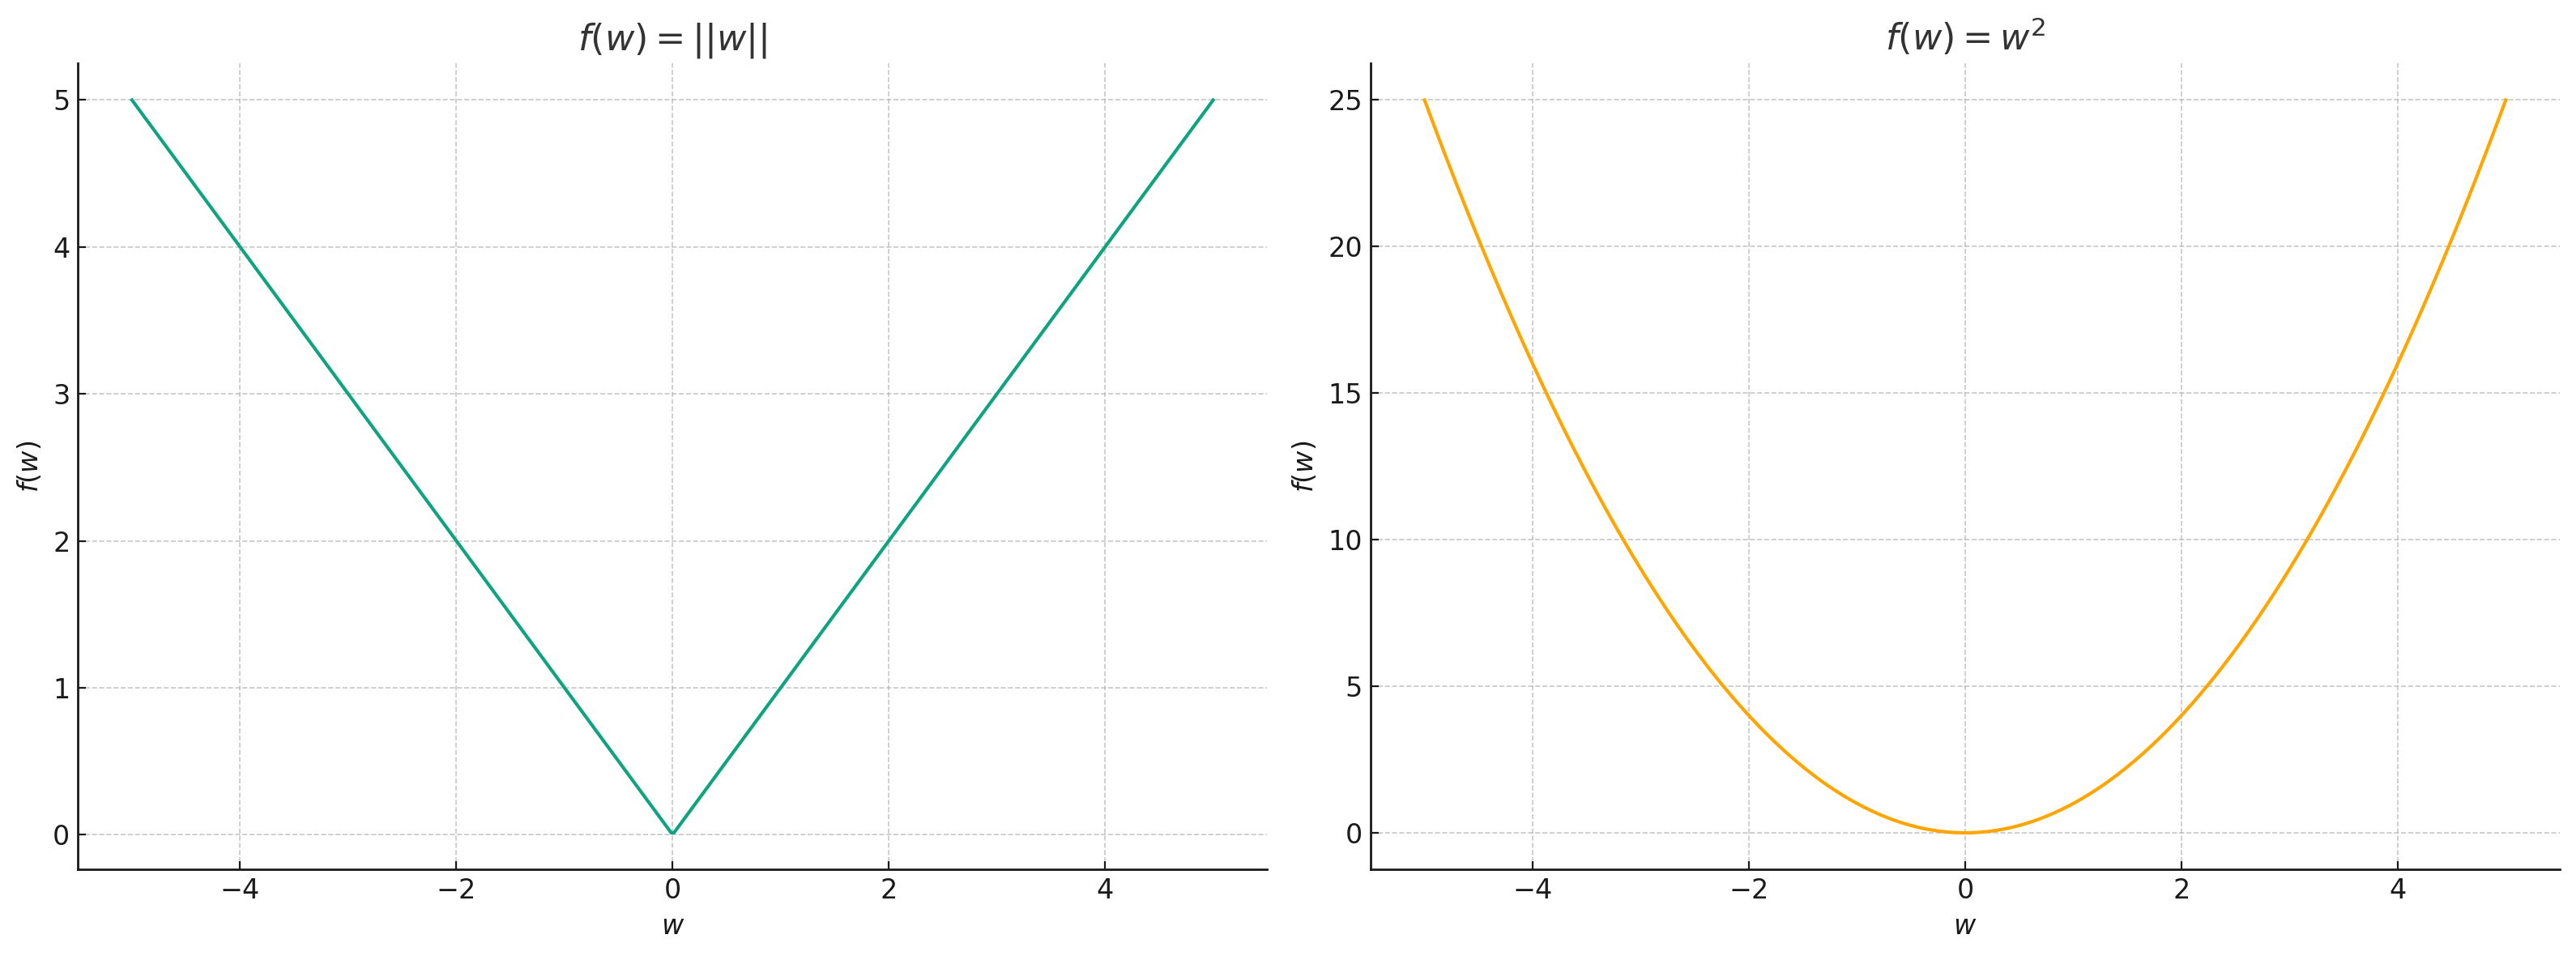
\includegraphics[width=100mm,scale=0.5]{images/regression_images/abs_w_vs_w_squared.png}
        
            \caption*{What's the derivative of $||w||$ at 0? We don't have one!}
        \end{figure}

        
        
    \phantom{}
        
    \subsection{Our Goal: Ordinary Least Squares}

        Now, we have the concepts we need.

        \begin{itemize}
            \item We want to \purp{minimize} loss $\loss$ on our data set, using the \gren{linear} model $\Theta$ ($h$).

            \item We'll use that linear model to \orgg{predict} the outputs of our data points.
        \end{itemize}
        
        This goal can be turned into an \purp{objective function}: $J(\Theta)=J(\theta,\theta_0)$
        
        \begin{equation}
            J(\theta,\theta_0) = \text{\pur{Training Loss}}
        \end{equation}

        Let's go step-by-step:

        \begin{itemize}
            \item Training loss is our \purp{expected loss}, averaged over each data point. $\red{\ex{g}{i}}$ is our prediction for $\blu{\ex{y}{i}}$.
            \note{Remember that $\blu{\ex{y}{i}}$ is the "correct" answer for our \grn{$\nth{i}$ data point}.}
        
        \begin{equation}
            J(\theta,\theta_0) = 
            \frac{1}{n}  \sum_{i=1}^n 
            \pur{\loss} ( \ex{g}{i},  \ex{y}{i}  )
        \end{equation}

            \item We'll use \gren{squared loss} to evaluate each data point:
        
        \begin{equation}
            J(\theta,\theta_0) = 
            \frac{1}{n}  \sum_{i=1}^n 
            \Big( \red{\ex{g}{i}}  - \blu{\ex{y}{i}} \Big)^{\grn{2}}
        \end{equation}

            \item We use our \textbf{hypothesis} $\red{h(} \blu{\ex{x}{i}} \red{;\Theta)}$ to make our guess $\red{\ex{g}{i}}$.
        
        \begin{equation}
            J(\theta,\theta_0) = 
            \frac{1}{n}  \sum_{i=1}^n 
            \left( 
                \red{h(} \blu{\ex{x}{i}} \red{;\Theta)} -  \ex{y}{i} 
            \right)^2 
        \end{equation}

            \item Our hypothesis is a \orgg{linear model} $\theta^T \blu{\ex{x}{i}}  + \theta_0$.\\
        \end{itemize}

        
        
        
        \begin{kequation}
            The \vocab{ordinary least squares} \vocab{objective function} for \purp{linear regression} is written as 
            \begin{equation*}
                J(\theta,\theta_0) = 
                \frac{1}{n}  \sum_{i=1}^n 
                \left( \red{ (\theta^T} \blu{\ex{x}{i}} \red{ + \theta_0) } 
                \quad-\quad \blu{\ex{y}{i}} \right)^2 
            \end{equation*}
        \end{kequation}
        
        If we break this into parts:
        
        \begin{equation}
            J(\theta,\theta_0) = 
                        \underbrace{
                            \frac{1}{n}  \sum_{i=1}^n 
                        }_{Averaging}
                        \left( 
                            \underbrace{
                                \red{ (\theta^T} \blu{\ex{x}{i}} \red{ + \theta_0) } 
                            }_{guess}
                            \quad-\quad 
                            \underbrace{
                                \blu{\ex{y}{i}}
                            }_{answer}
                        \right)^2 
        \end{equation}
        
        Now, this is an \purp{optimization} problem. We need to find the model $(\theta, \theta_0)$, that gives us the best (minimal) $J$.
            \note{We now have two parameters in our argmin function, but aside from listing both of them, the notation is the same. We just substituted $\Theta = (\theta, \theta_0)$}
        
        \begin{equation*}
            \theta^*, \theta_0^* = \argmin{\theta, \theta_0}{J(\theta,\theta_0)}
        \end{equation*}

        \phantom{}
        
    \subsection{Visualizing our Model}
    
        We'll start with the \vocab{one-variable} case. With one input, one output, we use a 2D plot to graph our data.

        \begin{itemize}
            \item Each piece of data is a simple $(x,y)$ pair: a \purp{point}.

            \item Meanwhile, our hypothesis is a \gren{line}: for each $x$, it predicts a different $y$.
        \end{itemize}
        
        \begin{figure}[H]
        \centering
            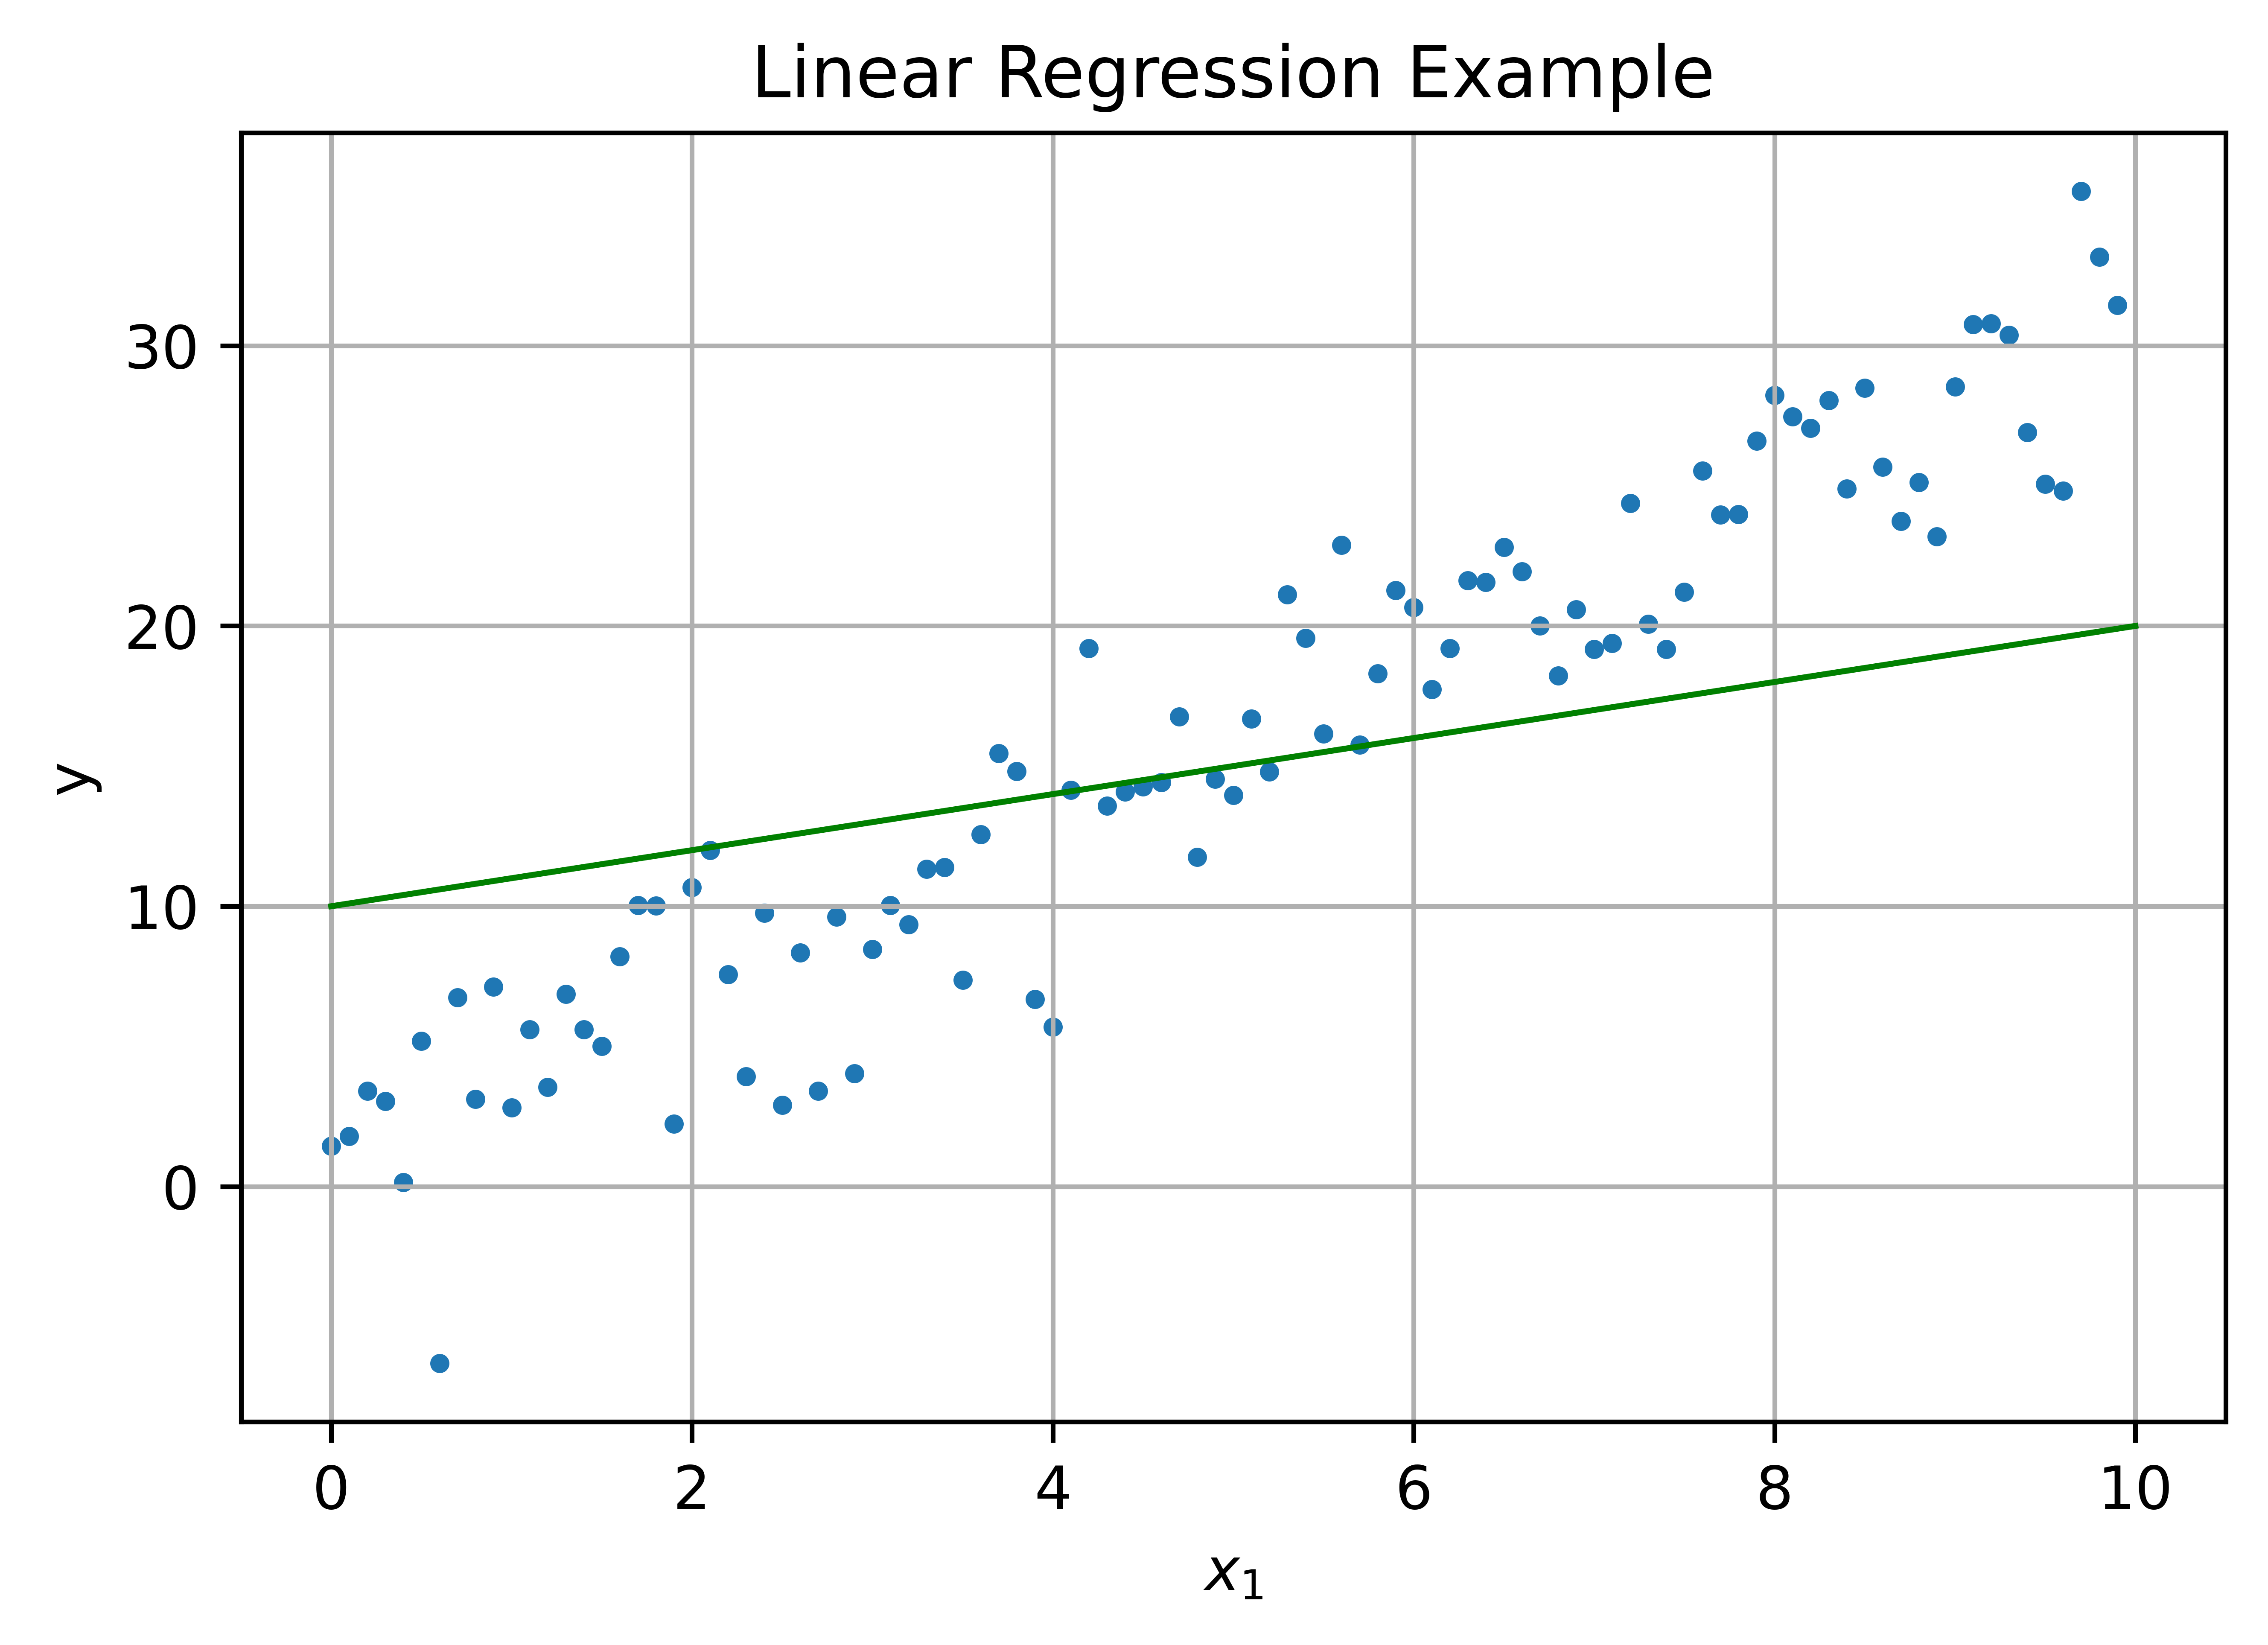
\includegraphics[width=70mm,scale=0.5]{images/regression_images/Regression_Example_Poor_Fit.png}
        
            \caption*{This linear model doesn't fit our data very well: $(\theta_0=10, \theta_1=1)$}
        \end{figure}

            \note{How do we know our line doesn't fit our data? Because it isn't "close" to the shape of the data.
            
            \phantom{}
            
            We want our model to really represent the data it comes from: they should look similar.}
        
        We're trying to get our line as \purp{close as possible} to the points, hoping to find a linear pattern. 
        
        \begin{itemize}
            \item We call this "\orgg{fitting}" our line to the data.
        \end{itemize}
        
        \begin{figure}[H]
        \centering
            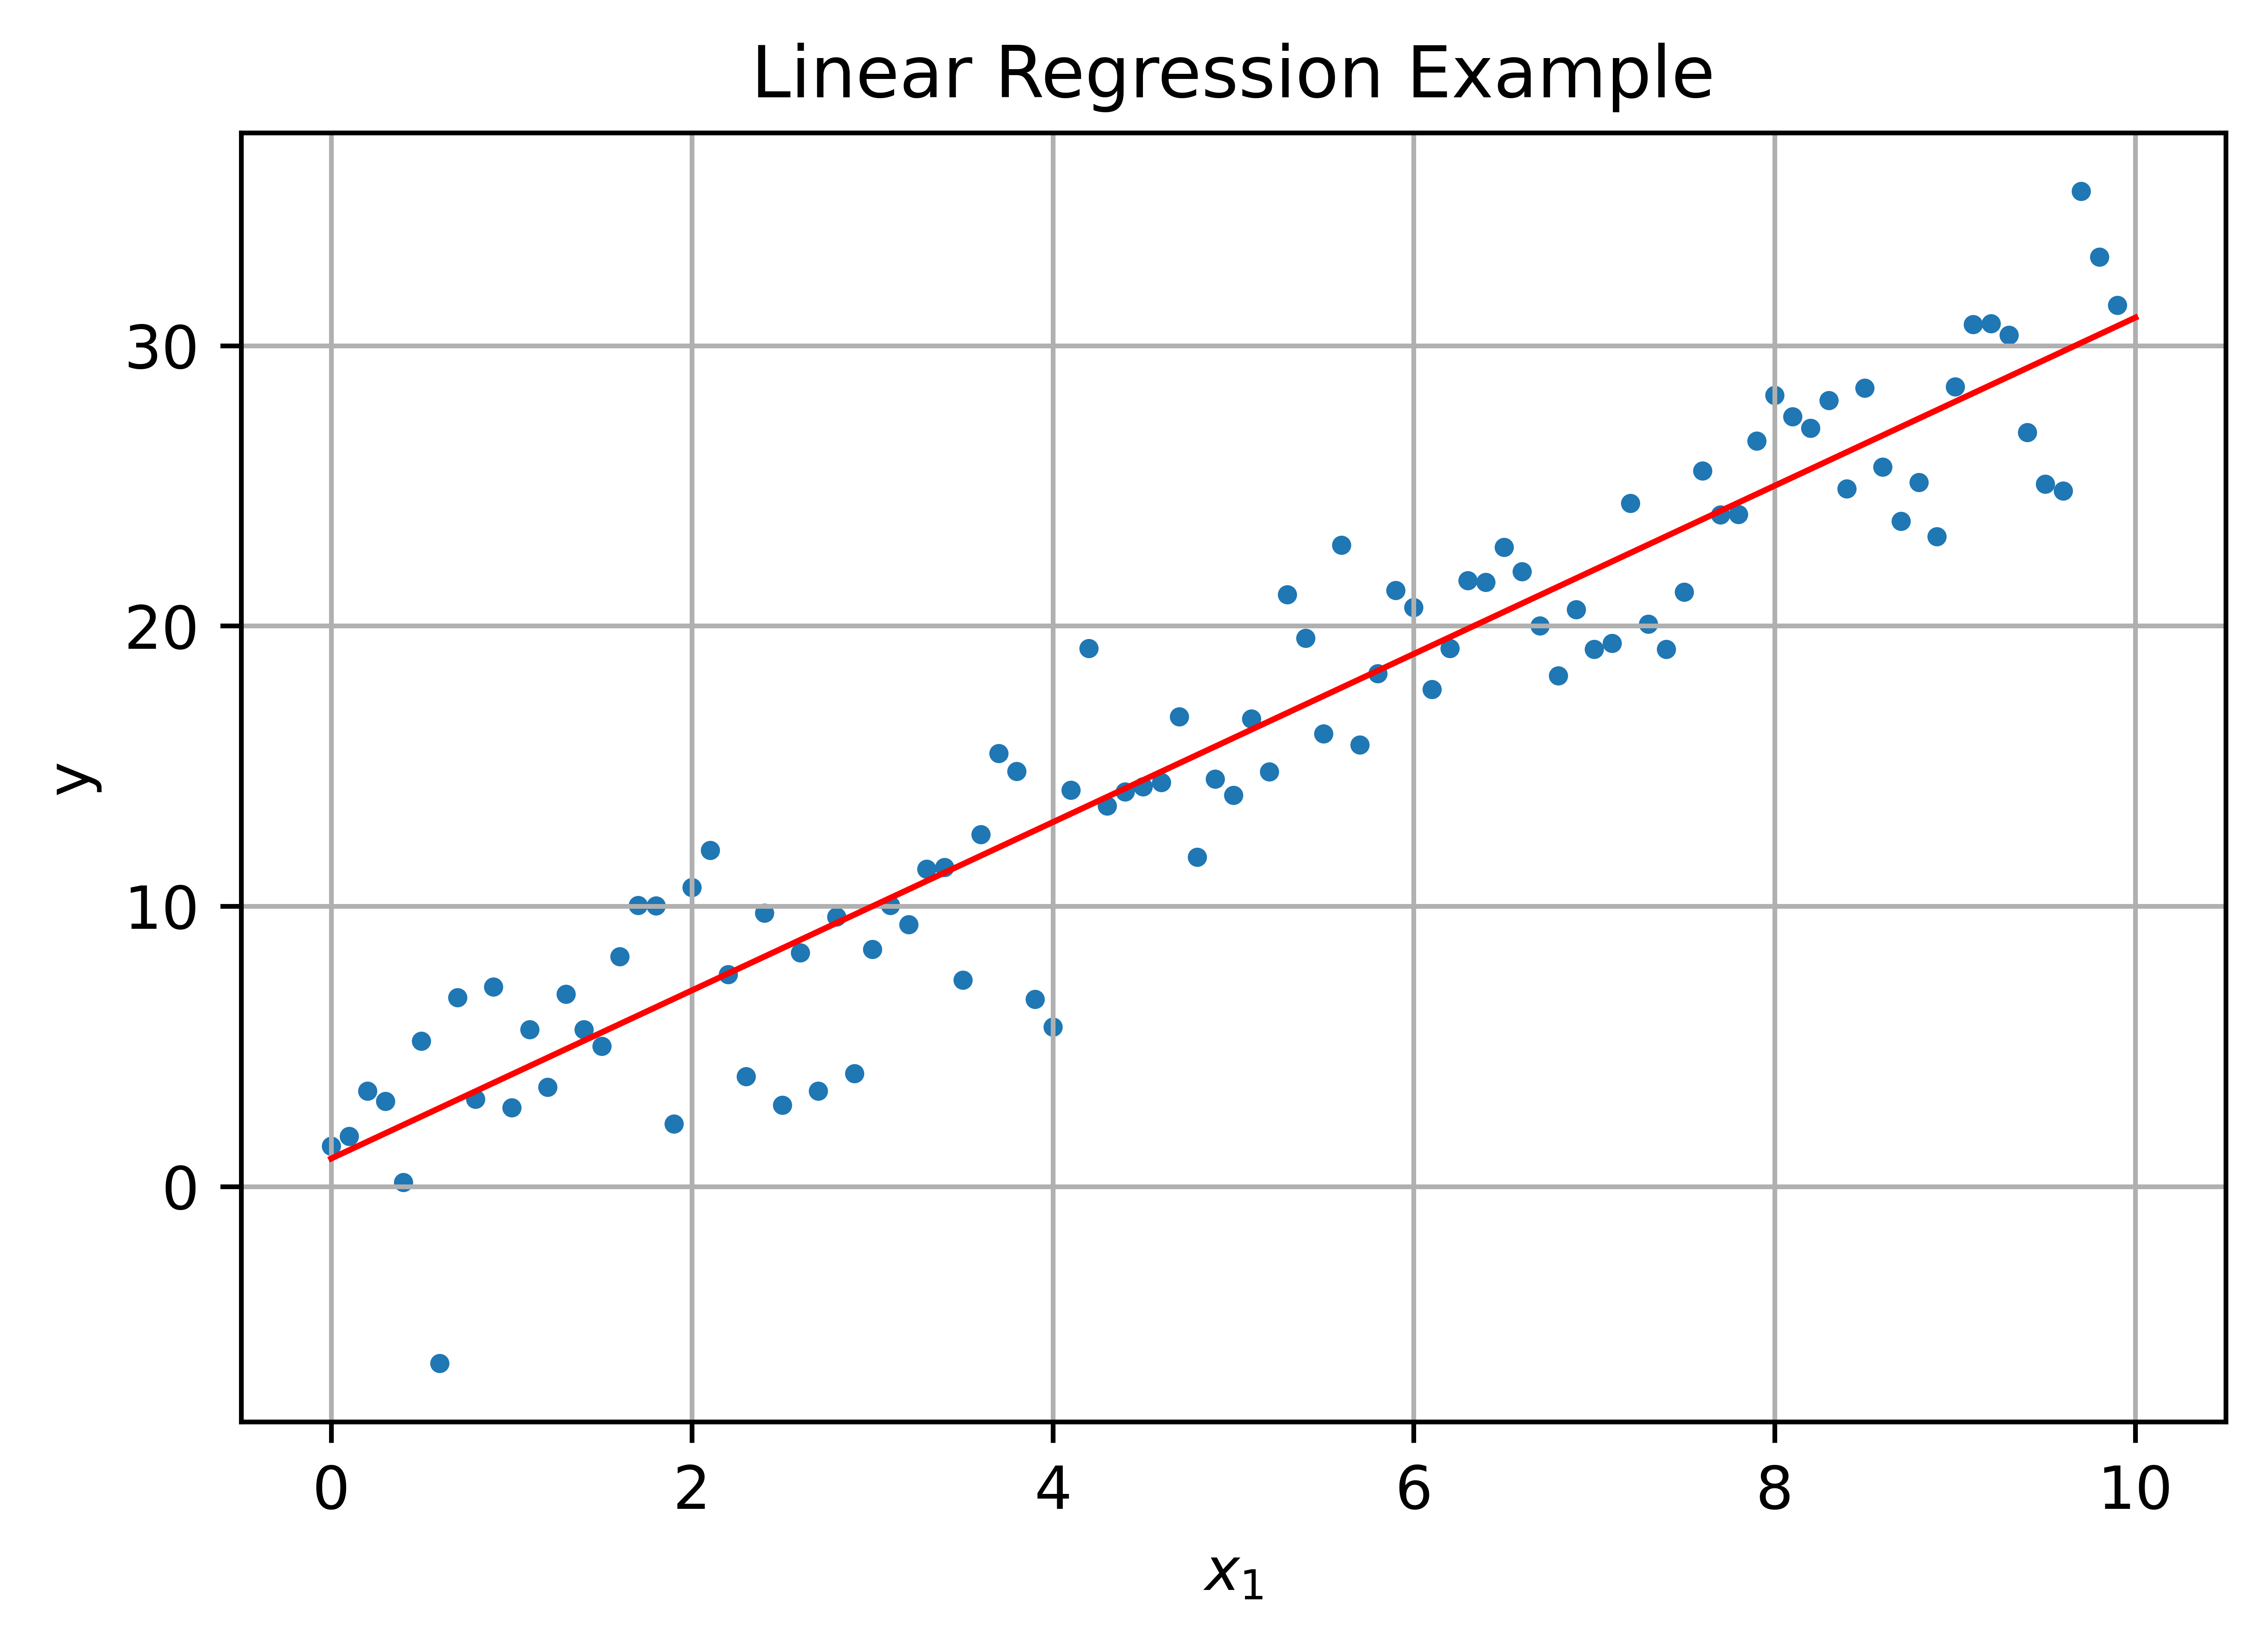
\includegraphics[width=70mm,scale=0.5]{images/regression_images/Regression_Example_Good_Fit.png}
        
            \caption*{This line is much better fitted to the data: $(\theta_0=1, \theta_1=3)$}
        \end{figure}
        
        What does this look like if we have \purp{two variables}? You need a 3D space, with 2 dimensions for the input.

        \begin{itemize}
            \item Each piece of data is a \purp{point} $(x_1,x_2, y)$.
            \item Our hypothesis is a \gren{plane}: for each pair $(x_1,x_2)$, it predicts a different $y$.
        \end{itemize}
        
        \begin{figure}[H]
        \centering
            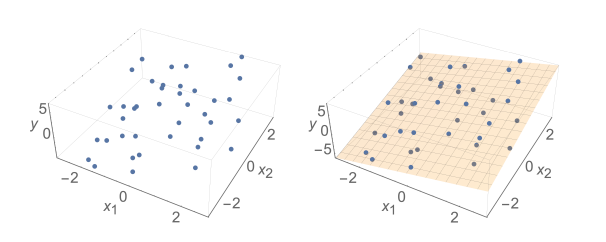
\includegraphics[width=100mm,scale=0.5]{images/regression_images/Regression_Plane.png}
        
            \caption*{This plane is \textbf{fitted} the same way our line was. Notice that $y$ is our \textbf{height}: this is the \textbf{output} of our regression.}
        \end{figure}
        
        Earlier, we mentioned that we can't really \purp{visualize} higher dimensions.
            \note{Looking at a 4D "plane" would be a headache.}
        
        \begin{itemize}
            \item So, instead, we don't even try to. We'll think of them in terms of our math. When we need intuition, we'll rely on the 2D plane.
            \item Because they're a higher-dimensional version of a \textbf{plane}, we call it a \vocab{hyperplane}.\\
        \end{itemize}
        
        \begin{definition}
            A \vocab{hyperplane} is a \purp{higher-dimensional version} of a \gren{plane} - a \gren{flat} surface that continues on forever.
            
            We use it to represent our \gren{linear} hypothesis for the purpose of \purp{regression}. 

            \begin{itemize}
                \item We have $d$ dimensions ($d$ variables) in our input.
                \item To represent our output, we need one additional, $\nth{(d+1)}$ dimension.
            \end{itemize}

            Visually, the "\purp{height}" of our plane represents the \orgg{output} of $h(x)$.
        \end{definition}

        \begin{itemize}
            \item Our line was a \textbf{1-D} object in a \textbf{2-D} plane.
            \item Our plane was a \textbf{2-D} object in a \textbf{3-D} space.
        \end{itemize}
        
        So, our \orgg{hyperplane} is a $d$ dimensional object in a $d+1$ dimensional space.

        \begin{itemize}
            \item Our goal is the same: we want our \vocab{hyperplane} to be as \textbf{close} to all of our data points as it possibly can.
        \end{itemize}

        
    \subsection{Another Interpretation}
    
        So far, we've generally interpreted our model similarly to $mx+b$.
        
        \begin{equation}
            h(x) = \red{\theta_0} + \red{\theta_1}x_1 + \red{\theta_2}x_2 + \red{\theta_3}x_3 + ... + \red{\theta_d}x_d
        \end{equation}

        \begin{itemize}
            \item Using our $\org{m}\grn{x}+b$ analogy, we can see $\org{\theta_k}$ as the "\orgg{slope}" of $\grn{x_k}$.

            \begin{equation}
                \pderiv{h}{x_k} = \theta_k
            \end{equation}
            
            \item In other words, $\theta_k$ tells us how much $x_k$ affects the \purp{output}.\\
        \end{itemize}

        \begin{concept}
            The \gren{larger} $||\theta_k||$ is, the \purp{more important} $x_k$ is to our output. 
            

            \begin{itemize}
                \item If we \gren{increase} $||\theta_k||$, then $x_k$ will have a \purp{bigger effect} on $h(x)$.
            \end{itemize}

            \begin{equation*}
                \overbrace{
                \pderiv{h}{x_k}
                }^{\text{Effect of $x_k$ on $h$}}= 
                \theta_k
            \end{equation*}

            This is a simple \orgg{pattern}: "as we change $x_k$, we change $h(x)$".
        \end{concept}

        We can also \gren{compare} each $\theta_k$ term to each other. 

        \begin{itemize}
            \item If $\theta_2$ is larger than $\theta_1$, then increasing $x_2$ would affect the output \orgg{more} than increasing $x_1$.

            \begin{equation}
                h(x) = 2x_1 + \overbrace{10000x_2}^{\text{$x_2$ has greater effect}}
            \end{equation}

            \item We could say that $x_2$ has a stronger effect on the output than $x_1$: it \gren{weighs more heavily} in the calculation.
        \end{itemize}
        
        
        Because of this, we sometimes call $\theta_k$ the \textbf{weight} for $x_k$.\\
        
        \begin{definition}
            A \vocab{weight} is a \orgg{parameter} that tells us how \gren{strongly} a variable influences our \purp{output}.
            
            It is usually a \purp{scalar} that we \gren{multiply} by our variable.
        \end{definition}

        \begin{itemize}
            \item We say that $\theta_0$ is an "offset", and the other $\theta_i$ terms are "weights".
        \end{itemize}

\pagebreak
%%%%%%%%%%%%%%%%%%%%%%%%%%%%%%%%%%%%%%%%%%%%%%%%%%%%%%%%%%%%%%%%%%%%%%%%%%%%%%%%%%%%%%%%%%%

\section{The stupidest possible linear regression algorithm}
    
    So, now we want to try to \purp{optimize} $J$ based on $\theta$ and $\theta_0$. How do we do that? Let's start as \gren{simple} as we possibly can.

    \phantom{}
    
    We can't try \textbf{every} possible $\Theta$, because there are an \purp{infinite} number of them. Rather than thinking too hard about a possible pattern, or an \textbf{algorithm}, let's just \orgg{randomly} try options.
    
    We'll try \textbf{random} values for $\theta$ and $\theta_0$, and \textbf{pick} whichever option gives us the \gren{best result}. Seems simple, if inefficient.

    \begin{figure}[H]
        \centering
            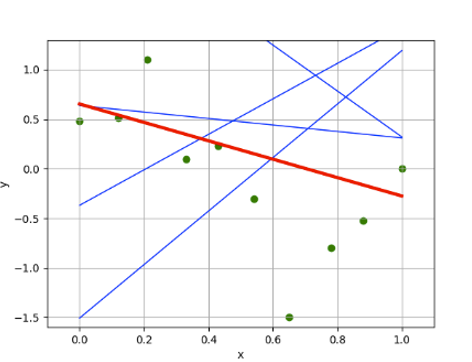
\includegraphics[width=70mm,scale=0.5]{images/regression_images/random_slopes.png}
        
            \caption*{Each line (hypothesis) was randomly generated. We focus on the red one: this is the best model, out of all the ones that we tried.}
        \end{figure}
    
    Why introduce such a silly algorithm? For a few reasons:
    
    \begin{itemize}
        \item It gives us an \textbf{example} of an optimization algorithm that's very \purp{simple}.
        \item \textbf{Randomly} generated results create a good \gren{baseline} - more intelligent algorithms can be compared to this one, to see how well we're doing.
            \note{Sometimes, you might come up with a clever technique, only to find out it isn't better than a random model! It happens more than you'd think.}
    \end{itemize}
    

\pagebreak
%%%%%%%%%%%%%%%%%%%%%%%%%%%%%%%%%%%%%%%%%%%%%%%%%%%%%%%%%%%%%%%%%%%%%%%%%%%%%%%%%%%%%%%%%%%

\section{Analytical solution: ordinary least squares}

    We can do \gren{better} than randomly \textbf{generate} parameters, though. In fact, in this rare case, we can actually \purp{solve} for optimal parameters!

    \phantom{}
    
    \subsection{Trying to Simplify}
        
        Our solution will involve a lot of algebra. Because of that, it's worth it to \gren{simplify} our formula as much as possible beforehand.
            \note{By algebra, we just mean "shuffling around math symbols in an equation".}
        
        \begin{equation}
            J(\theta,\theta_0) = 
                        \frac{1}{n}  \sum_{i=1}^n 
                        \left( 
                                \red{ (\theta^T} \blu{\ex{x}{i}} \red{ + \theta_0) 
                            }
                            - 
                                \blu{\ex{y}{i}}
                        \right)^2 
        \end{equation}
        
        Most parts of this equation can't really be \textbf{simplified}: $y$ and $x$ are just variables, and we can't do anything with the \textbf{sum} without knowing our data points.

        \begin{itemize}
            \item But, there's one notable detail: we \purp{separated $\theta_0$} from our other $\theta_k$ terms. 
            \item If we can \orgg{include $\theta_0$} in the dot product, our math will be easier.
        \end{itemize}
        

    \phantom{}
        
    \subsection{Combining $\theta$ and $\theta_0$}
        
         Let's go back to our \textbf{original} equation for $ (\theta^T x  + \theta_0)  $, before we switched to \purp{vectors}.
            \note{We drop the $\ex{}{i}$ notation whenever it isn't necessary, to de-clutter the equations. 
            
            \phantom{}
            
            Let's just say we've picked one random data point.}
        
        \begin{equation}
            h(x) \quad=\quad 
             \theta_0  + \theta \cdot x
            \quad=\quad 
            \red{\theta_0} + \theta_1x_1 + \theta_2x_2 + \theta_3x_3 + ... + \theta_dx_d
        \end{equation}
        
            We simplified our notation with a \gren{dot product}: each $\theta_k$ term is \textbf{multiplied} by an $x_k$ term.

        \begin{itemize}
            \item This is, of course, \orgg{excluding $\theta_0$}.
            \item We would end up with a simpler result if we could include $\theta_0$ in the $\theta$ vector. But, $\theta_0$ would need to be \purp{multiplied by an $x_0$ term}.
        \end{itemize}

        \begin{equation}
            h(x) = 
            \begin{bmatrix}
                \red{\theta_0} \\ \theta_1 \\ \vdots \\ \theta_d 
            \end{bmatrix}
            \cdot
            \overbrace{
            \begin{bmatrix}
                \blu{x_0} \\ x_1 \\ \vdots \\ x_d
            \end{bmatrix}
            }^{\text{We need $x_0$}}
        \end{equation}
        
        We have a trick: let's factor out \orgg{$x_0=1$}.
                    \note{You can always factor out 1 without changing the value!}
        
        
        \begin{equation}
            h(x) = \red{\theta_0}\blu{x_0} + \theta_1x_1 + \theta_2x_2 + \theta_3x_3 + ... + \theta_dx_d
        \end{equation}
        
        So, this means we just have to \textbf{append} a 1 to our vector $x$. At the \textbf{same time}, we'll append $\theta_0$ to $\theta$!
        
        \begin{equation}
            x = 
            \begin{bmatrix}
              \blu{1} \\ x_1 \\ x_2  \\ \vdots \\ x_d
            \end{bmatrix},
            \;\;\;\;\;\;\;\;\;\;\;\;\;\;\;
            \theta = 
            \begin{bmatrix}
              \red{\theta_0} \\ \theta_1 \\ \theta_2  \\ \vdots \\ \theta_d
            \end{bmatrix},
            \;\;\;\;\;\;\;\;\;\;\;\;\;\;\;
            h(x) = 
            \begin{bmatrix}
              \red{\theta_0} \\ \theta_1 \\ \theta_2  \\ \vdots \\ \theta_d
            \end{bmatrix}
            \cdot
            \begin{bmatrix}
              \blu{1} \\ x_1 \\ x_2 \\ \vdots \\ x_d
            \end{bmatrix}
        \end{equation}

        We'll write that symbolically, and then apply a transpose.
        
        \begin{equation}
            h(x) = \red{\theta} \cdot x = \blu{ \theta^T x }
        \end{equation}
        
        \begin{concept}
            Sometimes, to simplify our algebra, we can \orgg{append $\theta_0$} to $\theta$. 
            
            To make this possible, we \purp{choose $x_0=1$}.
            
            \begin{itemize}
                \item This requires \orgg{appending} a value of 1 to $x$.
            \end{itemize}
            
            Once we do this, we can \gren{write} 
            
            \begin{equation*}
                h(x)=\theta^T x
            \end{equation*}
        \end{concept}
        
        We \textbf{have} to append this 1 to every single $\ex{x}{i}$ in order for this to \textbf{work}. But, now we can treat our \gren{parameters} as \purp{one vector}.



    \pagebreak
    
    \subsection{Combining data points}

        There's another place we can clean things up:

        \begin{itemize}
            \item Currently, when using our \purp{objective} function, we have to \gren{sum} over \textbf{every} single data point.
                \note{Note that, for convenience, we've included $\theta_0$ in $\theta$.}
        \end{itemize}
    
        \begin{equation}
            J(\theta) = 
            \frac{1}{n}  \sum_{i=1}^n 
            \Big( \red{\theta^T} \blu{\ex{x}{i}}  - \blu{\ex{y}{i}}   \Big)^2
        \end{equation}

        \begin{itemize}
            \item This is a bit of a hassle - we have to consider every ($\ex{x}{i}, \ex{y}{i})$ term separately.

            \item Is there a better way?
        \end{itemize}
        
        We've solved this kind of problem before: using vectors above, we were able to work with \gren{many parameters} $\theta_k$ and \gren{many variables} $x_k$ at the same time.

            \begin{equation*}
            h(x) = \red{\theta_0} + \red{\theta_1}x_1 + \red{\theta_2}x_2 + \red{\theta_3}x_3 + ... + \red{\theta_d}x_d
            \xlongrightarrow{\text{vector form}} \quad
            h(x) = \theta^Tx
        \end{equation*}
        
        \begin{itemize}
            \item This made it easier to do lots of math quickly.\\
        \end{itemize}

        \begin{concept}
            One of the biggest benefits of \purp{matrices} is being able to do \gren{lots of math at the same time}.

            \begin{itemize}
                \item In particular, \vocab{matrix multiplication} allows you to do \gren{addition} and \purp{multiplication} on as many elements as you want.
            \end{itemize}
        \end{concept}
        
        Can we do the \textbf{same} here - combining \orgg{many data points} into one object?

    \phantom{}

    \subsection{Many data points in a matrix}

        We want to combine all of our data points into a single matrix. 

        \begin{itemize}
            \item We're already using \purp{rows} to represent \purp{multiple dimensions} of a data point. 
                \note{A reminder: a "dimension"(feature) is one aspect of our input data. For an animal, it might be height, weight, age, etc.
                
                \phantom{}
                
                Each dimension stores one piece of information.}

            \begin{equation}
                x = 
                    \begin{drcases}
                        \begin{bmatrix}
                            x_1 \\ x_2 \\ \vdots \\ x_d
                        \end{bmatrix}
                    \end{drcases}
                \text{ \lblu{ $\nth{k}$ dimension in row $k$} }
            \end{equation}

            \item We'll need different notation to separate \gren{data points}: we'll use \gren{columns}.
        \end{itemize}
    
        \begin{equation}
            X_{1D} =
                \overbrace{
                \begin{bmatrix}
                  \ex{x}{1} & \ex{x}{2} & \ex{x}{3} & \cdots & \ex{x}{n}
                \end{bmatrix}
                }^{\text{ \lblu{$\nth{i}$ data point in column $i$} }}
        \end{equation}
    
        \begin{definition}
            We use \purp{rows} to indicate the different \purp{dimensions} $x_k$ of a single data point, and \gren{columns} to indicate each \gren{data point} $\ex{x}{i}$.
    
            \begin{equation*}
                x = 
                    \begin{bmatrix}
                        \pur{x_1} \\ \pur{x_2} \\ \vdots \\ \pur{x_d}
                    \end{bmatrix}
                \qquad \qquad
                X_{1D} =
                    \begin{bmatrix}
                      \grn{\ex{x}{1}} & \grn{\ex{x}{2}} & \cdots & \grn{\ex{x}{n}}
                    \end{bmatrix}
            \end{equation*}
    
            \begin{itemize}
                \item Note that the capitalized $X$ matrix is used for \orgg{all of our data points $\ex{x}{i}$}.
            \end{itemize}
        \end{definition}

        \phantom{}

        These formats are both useful, but limited:

        \begin{itemize}
            \item $x$ can handle \purp{many dimensions}, but represents \gren{one data point}.
            \item $X_{1D}$ represents \gren{many data points}, but with only \purp{one dimension} for each.
        \end{itemize}

        Our solution? Combine them into a single object:\\

        \begin{kequation}
            $X$ is our \vocab{input matrix} in the shape \orgg{$(d \times n)$} contains information \gren{$n$ data points} with \purp{$d$ dimensions each}.
            
            \begin{equation*}
                X = 
                    \overbrace{
                        \begin{bmatrix}
                            \ex{x_1}{1} & \cdots  & \ex{x_1}{n} \\
                            \vdots      & \ddots & \vdots      \\
                            \ex{x_d}{1} & \cdots  & \ex{x_d}{n}
                        \end{bmatrix}
                        }^{ n \text{ data points}}
                    \bigggrB{50pt} d \text{ dimensions}
            \end{equation*}

        \end{kequation}

        \miniex Consider 3 data points in 2 dimensions: $[1,2]^T$, $[9,5]^T$, $[10,11]^T$.

        \begin{equation}
            \begin{bmatrix}
                1 \\ 2
            \end{bmatrix}, \;
            \begin{bmatrix}
                9 \\ 5
            \end{bmatrix}, \; 
            \begin{bmatrix}
                10 \\ 1
            \end{bmatrix}
            \quad \longrightarrow \quad 
            X = 
            \begin{bmatrix}
                1 & 9 & 10 \\
                2 & 5 & 1
            \end{bmatrix}
        \end{equation}

        If we want to replace $\theta^Tx +\theta_0$ with $\theta^Tx$, we can include 1's at the top:
            \note{Or the bottom, if we want.}

        \begin{equation}
            X = 
                \overbrace{
                    \begin{bmatrix}
                        1           & \cdots & 1           \\
                        \ex{x_1}{1} & \cdots  & \ex{x_1}{n} \\
                        \vdots      & \ddots & \vdots      \\
                        \ex{x_d}{1} & \cdots  & \ex{x_d}{n}
                    \end{bmatrix}
                    }^{ n \text{ data points}}
                \bigggrB{70pt} d+1 \text{ dimensions}
        \end{equation}
        
        We can do the same for $Y$: combine all of the data points into one matrix.\\
        
        \begin{kequation}
            $Y$ is our \vocab{output matrix} in the shape \purp{$(1 \times n)$} that contains all data points.
            
            \begin{equation*}
                Y = 
                    \begin{bmatrix}
                        \ex{y}{1} & \cdots & \ex{y}{n}
                    \end{bmatrix}
            \end{equation*}
        \end{kequation}

            \note{Why is this a row vector, not a matrix? 
            
            \phantom{}

            This is a \purp{regression} problem: each output is a scalar, not a vector!}

    \pagebreak

    \subsection{Objective Function in matrix form}

        Now that we can use all of our \gren{data points} at the same time, we can condense our objective function.

        \begin{equation}
            J(\Theta) = 
            \frac{1}{n}  \sum_{i=1}^n 
            \Big( \red{\theta^T} \blu{\ex{x}{i}}  - \blu{\ex{y}{i}}   \Big)^2
        \end{equation}

        We can simultaneously compute $(\red{\theta^T} \blu{\ex{x}{i}}  - \blu{\ex{y}{i}})$ for all of our data points at the same time:
            \note{We could show that this matrix multiplication gives the results we want, with calculation.
            
            \phantom{}
            
            But this is a little tedious, and doesn't teach us much, so we recommend trying it yourself if you're unconvinced.}

        \begin{equation*}
            \red{\theta^T} \blu{X} - \blu{Y}  \qquad=\qquad 
            \begin{bmatrix}
                \theta^T \ex{x}{\grn{1}}  - \ex{y}{\grn{1}} &&&
                \theta^T \ex{x}{\red{2}}  - \ex{y}{\red{2}} &&&
                \cdots &&&
                \theta^T \ex{x}{\org{n}}  -  \ex{y}{\org{n}}
            \end{bmatrix}
        \end{equation*}

        This isn't exactly what we want, though: we want $(\red{\theta^T} \blu{\ex{x}{i}}  - \blu{\ex{y}{i}})^2$: multiplied by itself. We can do this with a \gren{dot product}:

        \begin{equation}
            \Big( \red{\theta^T} \blu{\ex{x}{i}}  - \blu{\ex{y}{i}} \Big)^2 
            \quad \longrightarrow \quad
            \Big( \red{\theta^T} \blu{X} - \blu{Y} \Big) \cdot 
            \Big( \red{\theta^T} \blu{X} - \blu{Y} \Big)
        \end{equation}

        How do we write this dot product with matrix multiplication?\\

        \begin{clarification}
            When $a$ and $b$ were \purp{column vectors}, we could take their dot product as $a^Tb$.

            \begin{equation*}
                a = 
                \begin{bmatrix}
                    a_1 \\ a_2 \\ \vdots \\ a_m
                \end{bmatrix}
                \quad 
                b = 
                \begin{bmatrix}
                    b_1 \\ b_2 \\ \vdots \\ b_m
                \end{bmatrix}
                \quad \implies \quad
                a \cdot b = a^Tb
            \end{equation*}

            But we have to do the opposite for \gren{row vectors} $p$ and $q$: we get $pq^T$.

            \begin{equation*}
                \begin{matrix}
                    p = 
                \begin{bmatrix}
                    p_1 & p_2 & \cdots & p_m
                \end{bmatrix} \\\\
                q = 
                \begin{bmatrix}
                    q_1 & q_2 & \cdots & q_m
                \end{bmatrix}
                \end{matrix}
                \quad \implies \quad
                p \cdot q = pq^T
            \end{equation*}
        \end{clarification}

            \note{Here, we're comparing $a^Tb$ to $ab^T$.}

        Because $(\red{\theta^T} \blu{X} - \blu{Y}) $ is a \purp{row vector}, we'll have to write it in the $pq^T$ format:

        \begin{equation}
            \Big( \red{\theta^T} \blu{\ex{x}{i}}  - \blu{\ex{y}{i}} \Big)^2 
            \quad \longrightarrow \quad
            \Big( \pur{\theta^T X - Y} \Big) 
            \Big( \pur{\theta^T X - Y} \Big)^T
        \end{equation}

        This formula represents our original objective function:

        \begin{equation}
            \frac{1}{n}\Big( \pur{\theta^T X - Y} \Big) 
            \Big( \pur{\theta^T X - Y} \Big)^T
            \quad=\quad
            \frac{1}{n}  \sum_{i=1}^n 
            \Big( \red{\theta^T} \blu{\ex{x}{i}}  - \blu{\ex{y}{i}}   \Big)^2
        \end{equation}

        

        \begin{kequation}
            Using $X$, $Y$, and $\theta$ can write our \gren{objective function} for \purp{multiple} variables and \purp{multiple} data points as
            
            \begin{equation*}
                J(\theta) = \frac{1}{n}
                    \Big( \red{ \theta^T X - Y} \Big)
                    \Big( \red{ \theta^T X - Y} \Big)^T
            \end{equation*}
        \end{kequation}

            \note{Because $n$ is a constant, we sometimes ignore it when we're minimizing $J(\Theta)$.}

        \phantom{}

        
        It is important to \textbf{remember} the \textbf{shape} of our objects, as well.\\
        
        \begin{concept}
            Our matrices have the shapes:
            
            \begin{itemize}
                \item $X$:        $(d \times n)$ - matrix
                \item $Y$:        $(1 \times n)$ - row vector\\
                
                \item $\theta$:   $(d \times 1)$ - column vector
                \item $\theta_0$: $(1 \times 1)$ - scalar\\
                
                \item $J$:        $(1 \times 1)$ - scalar
            \end{itemize}
            
            If we combine $\theta_0$ into $\theta$, replace every use of \red{$d$} with \blu{$d+1$}.
            
        \end{concept}
        
        \note{Notice that these shapes make sense for our above equation! Try working through the matrix multiplication to verify this.}
        
        These shapes are worth \textbf{memorizing}.

        \phantom{}
        
    \subsection{Alterate Notation}
    
        One side problem: some ML texts use the \textbf{transpose} of $X$ and $Y$.\\
    
        \begin{notation}
            Some subjects use \vocab{different notation} for \vocab{matrices}. The main difference is that $X$ and $Y$ use their \purp{transpose}, which we'll notate as
        
            \begin{equation*}
                \Xt = X^T \;\;\;\;\;\;\;\; \Yt = Y^T
            \end{equation*}
            
            Thus, our equation above becomes
            
            \begin{equation*}
                J = \frac{1}{n}
                    \Big( \red{ \Xt \theta  - \Yt } \Big)^T
                    \Big( \red{ \Xt \theta  - \Yt } \Big) 
            \end{equation*}
        \end{notation}

    \pagebreak
        
    \subsection{Optimization in 1-D - Using Calculus}

        Now that we've sorted our data, we can start \purp{optimizing} $\theta$. Our goal is to modify $\theta$, to find the minimal $J$.
            \note{We're gonna focus on one data point/dimension at a time, so we don't need our matrix notation.}

        \begin{equation}
                J(\theta) = 
                \frac{1}{n}  \sum_{i=1}^n 
                \left( \red{\theta^T} \blu{\ex{x}{i}}  
                - \blu{\ex{y}{i}} \right)^2 
            \end{equation}
        
        We'll start with a simplified case, and build our way up:

        \begin{itemize}
            \item First, we limit our attention to one data point ($n=1$):

                \begin{equation}
                    J(\theta) =(\red{ \theta^T} \blu{x}   - \blu{y} )^2
                \end{equation}

            \item And we'll assume $\theta$ and $x$ are one-dimensional ($d=1$).

                \begin{equation}
                    J(\theta) = (\red{\theta} \blu{x}   - \blu{y} )^2
                \end{equation}
        \end{itemize}

        \phantom{}
        
        
        If we use $\theta$ as a \textbf{variable}, this is an ordinary single-variable function! How would we find the \purp{minimum}? 

        \begin{itemize}
            \item Using \textbf{calculus}! Anywhere there's a local \textbf{minimum}, we typically know the \gren{derivative is 0}.
                \note{Assuming a "smooth" surface...}\\
        \end{itemize}

        \begin{concept}
            
            If our function $J(\theta)$ has \gren{one variable}, we find possible \vocab{local minima} $\theta$ wherever the \purp{derivative} $\pderivslash{J}{\theta}$ is zero.
            
            \begin{equation*}
                \pderiv{J}{\theta}=0
            \end{equation*}

            \phantom{}

            \begin{itemize}
                \item To make sure it's a minimum (not a maximum), we also need to make sure that the \orgg{second derivative} is positive ($J''(\theta)>0)$.

                \item We already know this is true for \purp{squared loss}, so we won't bother with this step.
            \end{itemize}
        \end{concept}

            \note{Why do we need $\pderivslash{J}{\theta}=0$? 
            
            \phantom{}
            
            If $\pderivslash{J}{\theta}>0$, then decreasing $\theta$ slightly would reduce $J$: there's a lower point nearby, so this isn't a minimum!
            
            \phantom{}
            
            If $\pderivslash{J}{\theta}<0$, increasing $\theta$ has the same effect.}

        \begin{itemize}
            \item Note that we're taking $\pderiv{}{\theta}$, \redd{not} $\pderiv{}{x}$.
            \item This is because our goal is to modify $\theta$ (our model), not $x$ (our data).
                \note{We want to train our model to match our data, not the other way around!}
        \end{itemize}

        Let's do this for our simple example:
        
        \begin{equation}
            J'(\theta) = 2\blu{x}(\red{\theta} \blu{x} - \blu{y} ) = 0
        \end{equation}
        
        We just find where the slope $J'(\theta)$ is 0, and solve for $\theta$!
            \note{Because this is the optimal $\theta$, we call it $\theta^*$.}
        
        \begin{equation}
            \theta^* = \frac{y}{x}
        \end{equation}

        

    \phantom{}
        
    \subsection{Optimizing for multiple variables}

        This time, we'll do \gren{one data point}, having \purp{$d$ dimensions}.

        \begin{itemize}
            \item This gets a bit tricky, because we have to do our math with \orgg{vectors}.
                \note{Because we only have one data point, we'll omit the $\ex{}{i}$ notation.}
        \end{itemize}
        
        \begin{equation}
            J(\theta) = (\red{ \theta^T x  } - y )^2
        \end{equation}
        
        We'll \textbf{optimize} this. In the \gren{one-dimensional} case, we wanted to set the \textbf{derivative} of $J$ to \purp{zero}, using a single $\theta$ variable.
        
        \begin{itemize}
            \item Now, we have \orgg{multiple variables} $\theta_k$ that we could optimize.

            \item How do we know when we've optimized all of them?
        \end{itemize} 

        Well, if we consider each dimension separately, $\theta_k$ would be optimized if 

        \begin{equation}
            \pderiv{J}{\theta_k} = 0
        \end{equation}
        
        
        So, maybe it would be reasonable to just set \purp{every} derivative to \textbf{zero}? 
        
        \begin{itemize}
            \item It turns out, the answer is \textbf{yes}! 
                \note{We can use the reasoning that we used for 1D:
                
                \phantom{}
                
                If one of our derivatives $\pderivslash{J}{\theta_k} > 0$, then we could decrease $\theta_k$ to find a nearby point which is "lower" than our current point: we don't have a minimum.
                
                \phantom{}
                
                Thus, every derivative must be 0.}
        \end{itemize}
        
        
        If every individual derivative $\pderivslash{J}{\theta_k}$ is zero, we have a potential minimum.\\
        
        \begin{concept}
            If our function $J(\theta)$ has \red{$d+1$} \gren{parameters}, we find possible \vocab{local minimum} $\theta$ anywhere that obeys the system of equations
            
            \begin{equation*}
                \begin{matrix}
                    \pderiv{J}{\theta_{\red{0}}} = 0 &&
                \pderiv{J}{\theta_{\red{1}}} = 0 &&
                \pderiv{J}{\theta_{\red{2}}} = 0 &&
                \dots &&
                \pderiv{J}{\theta_{\red{d}}} = 0
                \end{matrix}
            \end{equation*}
            
            Or in general, 
            
            \begin{equation*}
                \pderiv{J}{\theta_{\red{k}}} = 0 \qquad \qquad \text{ for all $k$ in $\setty{0, 1, 2, \dots, d }$}
            \end{equation*}

            \begin{itemize}
                \item Why $d+1$ parameters instead of $d$? Because we're including $\theta_0$ as one additional parameter.
            \end{itemize}
            
        \end{concept}
        
        \note{Again, we ignore the second requirement of making sure this isn't a \textbf{maximum} or \textbf{saddle} point.}
        
        The \purp{solution} to this system of equations will be our \textbf{desired list of parameters}, $\theta^*$.

        \begin{equation}
            \theta^* = 
            \begin{bmatrix}
                \theta^*_1 \\ \theta^*_2 \\ \vdots \\ \theta^*_d
            \end{bmatrix}
        \end{equation}

    \phantom{}
        
    \subsection{Gradient Notation}

        Above, we wrote our derivative \purp{element-wise}: each derivative got its own equation.

        \begin{itemize}
            \item We can make things easier by storing our derivatives in a \orgg{column vector}, just like how $\theta$ stores $\theta_k$ terms.
                \note{How do we know that this is a column vector, and not a row vector? 
                
                \phantom{}
                
                Check out the matrix derivative notes for a complete explanation.}
        \end{itemize}

        \begin{equation}
            \pderiv{J}{\theta} = 
            \begin{bmatrix}
                \pderivslash{J}{\theta_0}\\
                \pderivslash{J}{\theta_1}\\
                \vdots \\
                \pderivslash{J}{\theta_d}\\
            \end{bmatrix}
        \end{equation}

        We'll think of this as a bigger, \gren{multivariable} derivative, called the \vocab{gradient}.
            \note{We'll give more conceptual intuition for the gradient in the next chapter. Look forward to it!}\\
        
        \begin{kequation}
            The \vocab{gradient} of $J$ with respect to $\theta$ is
            
            \begin{equation*}
                \nabla_\theta J 
                \quad=\quad
                \pderiv{J}{\theta} 
                \quad=\quad
                \begin{bmatrix}
                    \pderivslash{J}{\theta_0} \\
                    \pderivslash{J}{\theta_1} \\
                    \vdots \\
                    \pderivslash{J}{\theta_d}
                \end{bmatrix}
            \end{equation*}

            It has the same dimensions $(d \times 1)$ as $\theta$.
        \end{kequation}

            \note{Why is $\pderivslash{J}{\theta}$ a $(d \times 1)$ matrix instead of $(1 \times d)$? 
            
            \phantom{}
            
            We don't have a special reason: it's a convention we've picked, that works well with the rest of our math.
            
            \phantom{}
            
            In fact, some other texts might do differently. To learn more about our rules, check the Matrix Derivatives notes.}
        
        Now, we can rewrite our previous rule, "every derivative is 0":
        
        \begin{equation}
            \nabla_\theta J =
            \begin{bmatrix}
                \pderivslash{J}{\theta_0} \\
                \vdots \\
                \pderivslash{J}{\theta_d}
            \end{bmatrix}
            = 
            \begin{bmatrix}
                0 \\
                \vdots \\
                0
            \end{bmatrix}
            =
            \vec{0}
        \end{equation}
        
        
        \begin{concept}
            If $\theta$ is a \purp{vector}, we can find possible \vocab{local minima} $\theta$ of $J(\theta)$ anywhere that the \gren{gradient} $\nabla_{\theta}J$ is zero. 
            
            \begin{equation*}
                \nabla_\theta J=\vec{0}
            \end{equation*}

        \end{concept}
        
        \note{Once again: we should check if it's a minimum. But we continue to ignore this caveat.}
        
        This is the general equation we \orgg{solve} to find $\theta^*$.



    \phantom{}
        
    \subsection{Matrix Calculus}

        Now, we return to the general case: \gren{$n$ data points}, each having \purp{$d$ dimensions}.

        \begin{equation*}
            J(\theta) = \frac{1}{n}
                \Big( \red{ \theta^T X - Y} \Big)
                \Big( \red{ \theta^T X - Y} \Big)^T
        \end{equation*}

        Using the "alternate" notation":
        
        \begin{equation}
            J = \frac{1}{n}
                \left( \blu{ \Xt \theta  - \Yt } \right)^T
                \left( \blu{ \Xt \theta  - \Yt } \right) 
        \end{equation}
        
        We will \purp{not} show how to take this matrix derivative. But our result is:
            \note{Want to know how? Check out A.4 in the official appendix.}

        \begin{equation}
            \nabla_\theta J = 
                \frac{2}{n} \Xt^T
                \left( \blu{ \Xt \theta  - \Yt } \right) 
            =0
        \end{equation}

        \begin{clarification}
            Note that matrix derivatives often look \gren{similar} to traditional, single-variable derivatives. However, they are \redd{not the same}.

            \begin{itemize}
                \item Often, this can result in \purp{shape errors}: we end up with the wrong matrix shape.
            \end{itemize}
        \end{clarification}

            \note{How do we take a matrix derivative in general? Check out an explanation in the Matrix Derivatives chapter.}
        
        
        From here, we just solve for $\theta$, using matrix multiplication rules.\\
        
        \begin{kequation}
        
            The \vocab{solution} for \vocab{OLS optimization} is 
            
            \begin{equation*}
                \theta = 
                \underbrace{ 
                \inv{ \left(  \Xt^T\Xt  \right)  }
                }_{d \times d}
                \underbrace{
                \Xt^T
                }_{d \times n}
                \underbrace{
                \Yt
                }_{n \times 1} 
            \end{equation*}
            
            Or, in our \purp{original} notation,
            
            \begin{equation*}
                \theta = 
                \underbrace{ 
                \inv{ \left(  XX^T  \right)  }
                }_{d \times d}
                \underbrace{
                X
                }_{d \times n}
                \underbrace{
                Y^T
                }_{n \times 1} 
            \end{equation*}

            \phantom{}

            \begin{itemize}
                \item If $\theta_0$ is included in $\theta$, then dimension $d$ is replaced with $d + 1$.
            \end{itemize}
            
        \end{kequation}

            \note{Note that this requires that $XX^T$ is invertible: we need to compute that inverse $(XX^T)^{-1}$ in the equation, after all.
            
            \phantom{}
            
            This technique doesn't work if that's not the case. But, we'll introduce a different technique to solve this problem: regularization!}

        
        
    We've finished with "ordinary least squares".
    
    \begin{itemize}
        \item We call it "ordinary" because this is the \gren{simple} version of the problem.
        \item We'll make it more complex by introducing \orgg{regularization}.
    \end{itemize}

        
\pagebreak
%%%%%%%%%%%%%%%%%%%%%%%%%%%%%%%%%%%%%%%%%%%%%%%%%%%%%%%%%%%%%%%%%%%%%%%%%%%%%%%%%%%%%%%%%%%

\section{Regularization}

    The above solution gives us the \gren{best} model for matching our \purp{training data}.

    \begin{itemize}
        \item But earlier, we mentioned that we want our model to be able to \orgg{generalize} to new data.
            \note{Because our training data doesn't perfectly reflect all of our future data.}
    \end{itemize}

    We need some math to represent this goal of "generality".

    \begin{itemize}
        \item This equation won't measure our performance on training data, but instead encourages us to do well on \purp{future data}.
    \end{itemize}
        
    We call this type of function a \vocab{regularizer}.\\
    
    \begin{definition}
        A \vocab{regularizer} is a term to our \gren{objective function} that helps measure how \purp{general} our hypothesis is.

        \begin{itemize}
            \item By \gren{optimizing} this term, we hope to create a model that works better with \purp{new data} we didn't train with.
        \end{itemize}
        
        This function takes in our \purp{vector of parameters} \gren{$\Theta$} as an input: \purp{$R(\Theta)$}.
    \end{definition}

    But how do we make a model "more general?"

    \begin{itemize}
        \item First, we need to \gren{understand} the problem: \purp{what's wrong} with only using our training data?
        
    \end{itemize}


    

    \phantom{}

    \subsection{Coincidences, and fake patterns}

        The goal of our model $\theta$ is to look for \purp{patterns}. This is a concept we discussed earlier (section 2.3.8):\\

        \begin{concept}
            \textit{(Review)}
            
            The \gren{larger} $||\theta_k||$ is, the \purp{more important} $x_k$ is to our output. 
            

            \begin{itemize}
                \item If we \gren{increase} $||\theta_k||$, then $x_k$ will have a \purp{bigger effect} on $h(x)$.
            \end{itemize}

            \begin{equation*}
                \overbrace{
                \pderiv{h}{x_k}
                }^{\text{Effect of $x_k$ on $h$}}= 
                \theta_k
            \end{equation*}

            This is a simple \gren{pattern}: "as we change $x_k$, we change $h(x)$ by this much".
        \end{concept}

        $\theta$ is trying to identify \orgg{which variables} have an effect on our output, and by how much.
            \note{$\theta_k<0$ doesn't mean that $x_k$ doesn't matter: it just means that it affects $h(x)$ by decreasing it, instead of increasing it.}

        \begin{itemize}
            \item If $||\theta_k||$ is large, our models thinks that $x_k$ is important to our output.
        \end{itemize}

        Our goal is to modify each $\theta_k$ term until it matches the real distribution.

        

        \phantom{}

        But seeing a pattern ($x_k$ affecting $h(x)$) doesn't mean that it's real: \purp{random chance} can cause us to see patterns that don't really exist.

        \begin{itemize}
            \item \miniex You take 20 quizzes during a semester. Every time you did \gren{well}, you happened to be wearing a \redd{red shirt}.
            
            \item You might come to believe that red shirts help you study \gren{better}, even though it was just luck.
        \end{itemize}

        Isn't this kind of coincidence a bit unlikely? Maybe. 

        \begin{itemize}
            \item But what happens if we have 10 possible coincidences? It's less likely that we avoid all of them.
                \note{Suppose the chance of one coincidence is $p$.
                
                \phantom{}
                
                The chance of \gren{one} coincidence not occurring is $(1-p)$. The chance of \purp{ten} coincidences not occurring is $(1-p)^{10}$.

                \phantom{}
                
                As we get more chances, we're more likely to see a coincidence.}

            \item In other words: the more \orgg{opportunities} there are for something rare to happen, the \gren{more likely} it is to happen.\\
        \end{itemize}


        \begin{concept}
            The more \gren{patterns} we're looking for, the more likely that \textbf{at least one} of the them shows up by \orgg{coincidence}.

            \begin{itemize}
                \item Our data can, by chance, match a pattern that \purp{isn't even real}. 
            \end{itemize}
        \end{concept}
        
            \note{For some entertaining examples, search the phrase "spurious correlation".}

        This really becomes a problem for our model: often, we \purp{don't know} what data matters, so we include \gren{everything} we possibly can.

        \begin{itemize}
            \item But the more data we include, the more likely that something looks \gren{important} on \orgg{accident}!
        \end{itemize}

        This is an interesting situation, where \gren{learning more} about our training data can cause our model to perform \purp{worse}: we're \vocab{overfitting}.
            \note{Learning more about our training data isn't necessarily the same as learning more about the true distribution that data came from!}\\

        \begin{definition}
            \textit{(Review from Introduction chapter)}

            \vocab{Overfitting} occurs whenever we \gren{learn} ("fit") our training data too exactly, and it causes problems when we see \purp{new data}.

            \begin{itemize}
                \item Often, we \orgg{memorize} very specific patterns, that don't actually hold up in general: they only appeared in our randomly sampled training data. 
            \end{itemize}
        \end{definition}

        \miniex You flip a coin 10 times, and it comes up heads 8 times.

        \begin{itemize}
            \item You've decided that the coin has an 80\% chance of coming up heads.

            \item But it's a fair coin: the 'training data' (10 coin flips) doesn't match the 'true distribution' (50\% chance of heads).
        \end{itemize}

        Now, we understand our problem. Let's come up with a solution.


    \phantom{}

    \subsection{Ridge Regression}

        We're worried about our model \purp{finding false patterns} based on weak evidence.

        \begin{itemize}
            \item If our model finds a \gren{pattern}, then it'll increase $||\theta_k||$: it considers $x_k$ to be important for predicting $h(x)$, because the data coincidentally makes it \purp{look} important.
        \end{itemize}

        If our model is "too eager" to find patterns, we can make it \orgg{more skeptical} of patterns it might see.
            \note{It still need to look for \textit{some} (hopefully real) patterns, so that it can make good predictions $h(x)$.}

        \begin{itemize}
            \item In other words, we'll \purp{punish} our model for increasing $||\theta_k||$ too easily.
                \note{We'll actually use $\theta_k^2$, for the same reasons we use squared loss: 
                
                \phantom{}
                
                Smoother, works well for positive and negative $\theta_k$, etc.}\\
        \end{itemize}

        \begin{concept}
            We want to \purp{discourage} our model from prematurely deciding that $x_k$ has a \orgg{effect} on $h(x)$.

            \begin{itemize}
                \item Thus, we'll \gren{discourage} our model from increasing $||\theta_k||$: $\pur{\theta_k}$ represents this "\orgg{effect}".
            \end{itemize}

            \begin{equation*}
                R(\theta_k) = \theta_k^2
            \end{equation*}

            \begin{itemize}
                \item Our algorithm will \purp{minimize} $R(\Theta)$, so we'll make this $\theta_k^2$ \gren{small}.
            \end{itemize}
        \end{concept}

        We can repeat this process for all of our $\theta_k$ terms, and combine them into a vector $\theta$:

        \begin{equation*}
            R(\Theta) = \sum_k \pur{\theta_k^2} 
            \quad=\quad \abs{|\theta|}^2 = \theta \cdot \theta
        \end{equation*}

        This is our \orgg{ridge regression} model.
            \note{Why "ridge regression"? We'll get into that later.}\\

        \begin{kequation}
            Our \redd{regularizer for regression} will be given by \purp{square magnitude} of $\theta$:
            
            \begin{equation*}
                R(\Theta) = \norm{\theta}^2 = \theta^T\theta
            \end{equation*}

            \begin{itemize}
                \item In this model, we are biasing $\norm{\theta}$ towards 0: the farther from 0 we are, the more we punish the model.
            \end{itemize}
            
            This approach is called \vocab{Ridge Regression}.
        \end{kequation}

    \phantom{}

    \subsection{$\lambda$, our regularization constant}

        We can now create an "\purp{objective function}" that includes training loss, \textbf{and} regression.

        \begin{equation}
            J(\theta) = 
                        \frac{1}{n}  \sum_{i=1}^n 
                        \left( 
                            \underbrace{
                                \red{(\theta^T \ex{x}{i}  
                                + \theta_0)}
                            }_{guess}
                            - \underbrace{
                                \blu{\ex{y}{i}} 
                            }_{answer}
                        \right)^2 
                        + 
                        \underbrace{
                            \pur{ \norm{\theta}^2 }
                        }_{Regularizer}
        \end{equation}

        Notice that these terms "compete" with each other:\\

        \begin{concept}
            Our \gren{training loss} and \purp{regularizer} compete with one another, affecting our model in opposing ways:

            \begin{itemize}
                \item Our regularizer wants us keep $\theta$ small, being more \gren{suspicious} of predicting patterns.

                \item But in order to make good predictions for our \purp{training data}, we need to find the \orgg{real} patterns: some $\theta$ values need to be bigger, to predict our data.
            \end{itemize}
        \end{concept}

            \note{This is why we don't end up with model $\theta=\vec{0}$: while this model would have low \purp{regularization} $R(\Theta)$, it'll have high \gren{training loss}.}


        We need a \gren{balance} between training loss and regularization. It would be useful to have a way to \orgg{control} that balance.

        \begin{itemize}
            \item That way, we can decide, "how much do we care about matching training data, versus avoiding coincidental patterns?"
        \end{itemize}

        We have a tool for this: we'll represent "how much we care about \redd{regularization}" with a \vocab{constant} \red{$\lambda$}.\\

        \begin{definition}
            \vocab{Lambda}, or \vocab{$\lambda$}, is the constant ($\lambda \geq 0$) we \gren{scale} our \purp{regularizer} by.

            \begin{equation*}
                \text{Total Regularization} \quad=\quad  \lambda R(\Theta) 
                \quad = \quad \lambda ||\theta||^2
            \end{equation*}
            
            It represents \gren{how strongly} we want to regularize: the larger it is, the more strongly we try to \purp{generalize} our model.

        \end{definition}

        Why is $\lambda \geq 0$?\\

        \begin{clarification}
            We keep $\lambda \geq 0$, because $\lambda<0$ would encourage our model to make $||\theta||$ \gren{bigger}, no matter what.

            \begin{itemize}
                \item There's a limit to how small $|\theta|$ can be, but there's \purp{no limit} on how big it can be: it would just keep getting bigger forever.
            \end{itemize}
        \end{clarification}

        Finally, we have our \purp{completed} objective function:\\

        \begin{kequation}
            The \vocab{objective function} for \vocab{ridge regression} is given as 
            
            \begin{equation*}
                J(\Theta) = 
                            \frac{1}{n}  \sum_{i=1}^n 
                            \left( 
                                \underbrace{
                                    \red{(\theta^T \ex{x}{i}  
                                    + \theta_0)}
                                }_{guess}
                                - \underbrace{
                                    \blu{\ex{y}{i}} 
                                }_{answer}
                            \right)^2 
                            + 
                            \underbrace{
                                \pur{ \lambda \norm{\theta}^2 }
                            }_{Regularizer}
            \end{equation*}
        \end{kequation}

            \note{Readers might catch that our regularizer doesn't include $\theta_0$. There's a good reason for that! We'll discuss it below.}

        Once again, we note the contrast between "training loss" and "regularization".

        \begin{itemize}
            \item We've only made one change: $\lambda$ can increase or decrease our focus on regularization.
        \end{itemize}

        This $\lambda$ is crucial to our model: the larger it is, the more we punish our model for increasing $||\theta||$.\\

        \begin{concept}
            The more \vocab{regularization} (large $\lambda$) we have, the more we're \purp{focused} on keeping $|\theta|$ small.

            \begin{itemize}
                \item If we make $\lambda$ \gren{too big}, then $||\theta||$ becomes \purp{very small}: our model doesn't learn enough information.

                \item If we make $\lambda$ \gren{too small}, then $||\theta||$ becomes \purp{very big}: our model learns \orgg{all} the patterns of our data, even the ones that come from random noise.
            \end{itemize}
        \end{concept}




    \pagebreak

    \subsection{Why not regularize $\theta_0$?}

        Note that when we regularize with $\pur{ \lambda \norm{\theta}^2 }$, we're \orgg{not including $\theta_0$} in our vector:

        \begin{equation}
            R(\Theta) = \lambda \theta^T\theta \qquad \qquad 
            \theta = \begin{bmatrix}
                \red{\theta_1} \\ \theta_2 \\ \vdots \\ \theta_d
            \end{bmatrix}
        \end{equation}

        This suggest that we're \purp{not regularizing} $\theta_0$. Why is that?\\

        \begin{concept}
            We \orgg{do not regularize} $\theta_0$.

            \begin{itemize}
                \item We \gren{allow} $\theta_0$ to take whatever value fits best.
            \end{itemize}
        \end{concept}

        The first reason: $\theta_0$ works \purp{differently} from our other $\theta_k$ terms.

        \begin{itemize}
            \item A term $\theta_k$ tell us how \gren{important} one variable $x_k$ is to our output $h(x)$.

            \item $\theta_0$ works almost the opposite way: it \orgg{ignores} our input $x$, and gives a baseline output.

                \begin{itemize}
                    \item In other words: if we \purp{remove} the effect of all of our variables ($x=\vec{0}$), what do we expect to see?
                        \note{If our input data is centered on $x=\vec{0}$ (equally above and below on each axis), $\theta_0$ is the \gren{average} output we expect to see.}
                \end{itemize}
        \end{itemize}

        Naturally, regularization has very different effects:

        \begin{itemize}
            \item If you regularize $||\theta_k||$, your model i will emphasize the \orgg{effect} of $x_k$ by a smaller amount. 
            
            \item If you regularize $||\theta_0||$, you've just \gren{shifted} every output, by the same amount.\\
        \end{itemize}

        \begin{concept}
            Unlike $\theta_k$, $\theta_0$ doesn't find \orgg{patterns} in the data: it just tells us roughly how \purp{large} our output is.

            \begin{itemize}
                \item In fact, $||\theta_0||$ affects all of our data in the \gren{exact same way}.

                \item Decreasing $||\theta_0||$ would shift all outputs equally: this doesn't do anything to make it more \gren{accurate} for future data.
            \end{itemize}

            Because of this difference, it's not necessary to \orgg{regularize} $\theta_0$.
        \end{concept}

        \phantom{}

        Another reason we don't regularize $\theta_0$ is that it's often \orgg{necessary} for good predictions. This is best shown with a \textbf{visual} example.

        \begin{itemize}
            \item Let's take an example with one input, $x_1$. So, we have a \purp{linear} function: \red{$h(x) = \theta_1x_1+\theta_0$}.
        \end{itemize}
        
        \begin{figure}[H]
        \centering
            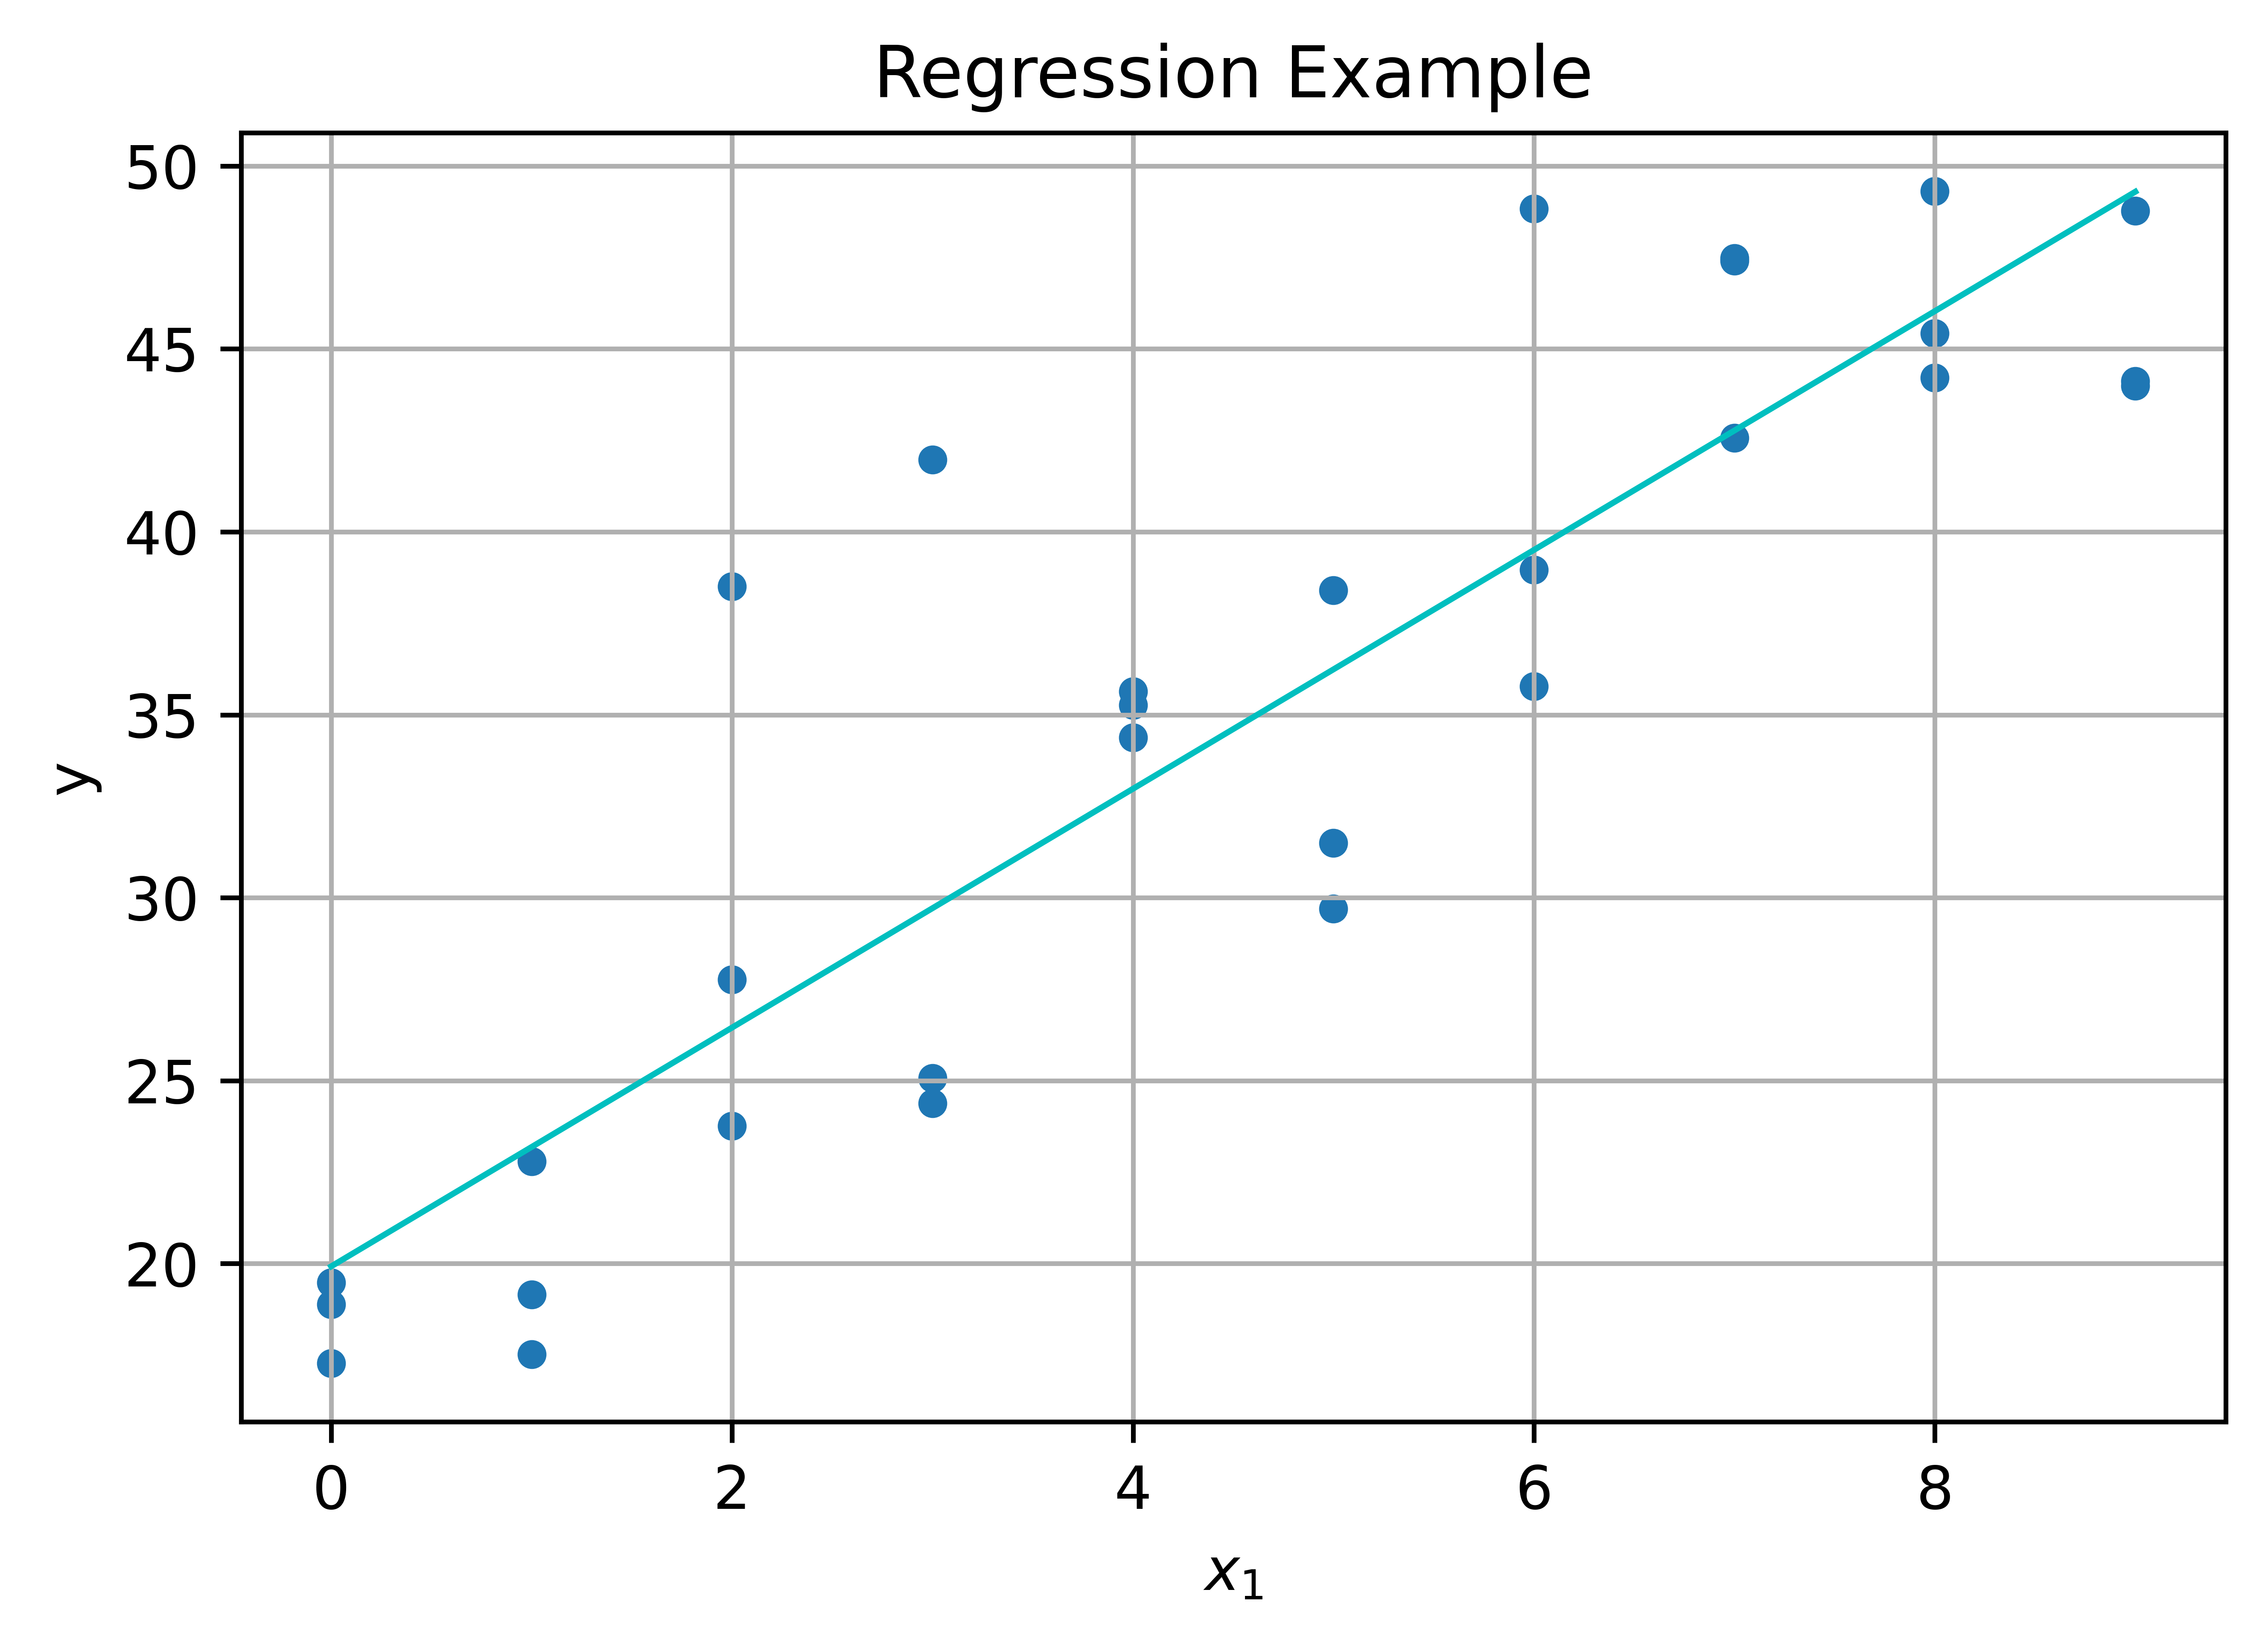
\includegraphics[width=70mm,scale=0.5]{images/regression_images/Regression_Keep_Offset.png}
        
            \caption*{Our regression example.}
        \end{figure}
        
        Let's suppose we \orgg{regularize}, or shrink, our offset $\theta_0$, while keeping everything else the same:
        
        \begin{figure}[H]
        \centering
            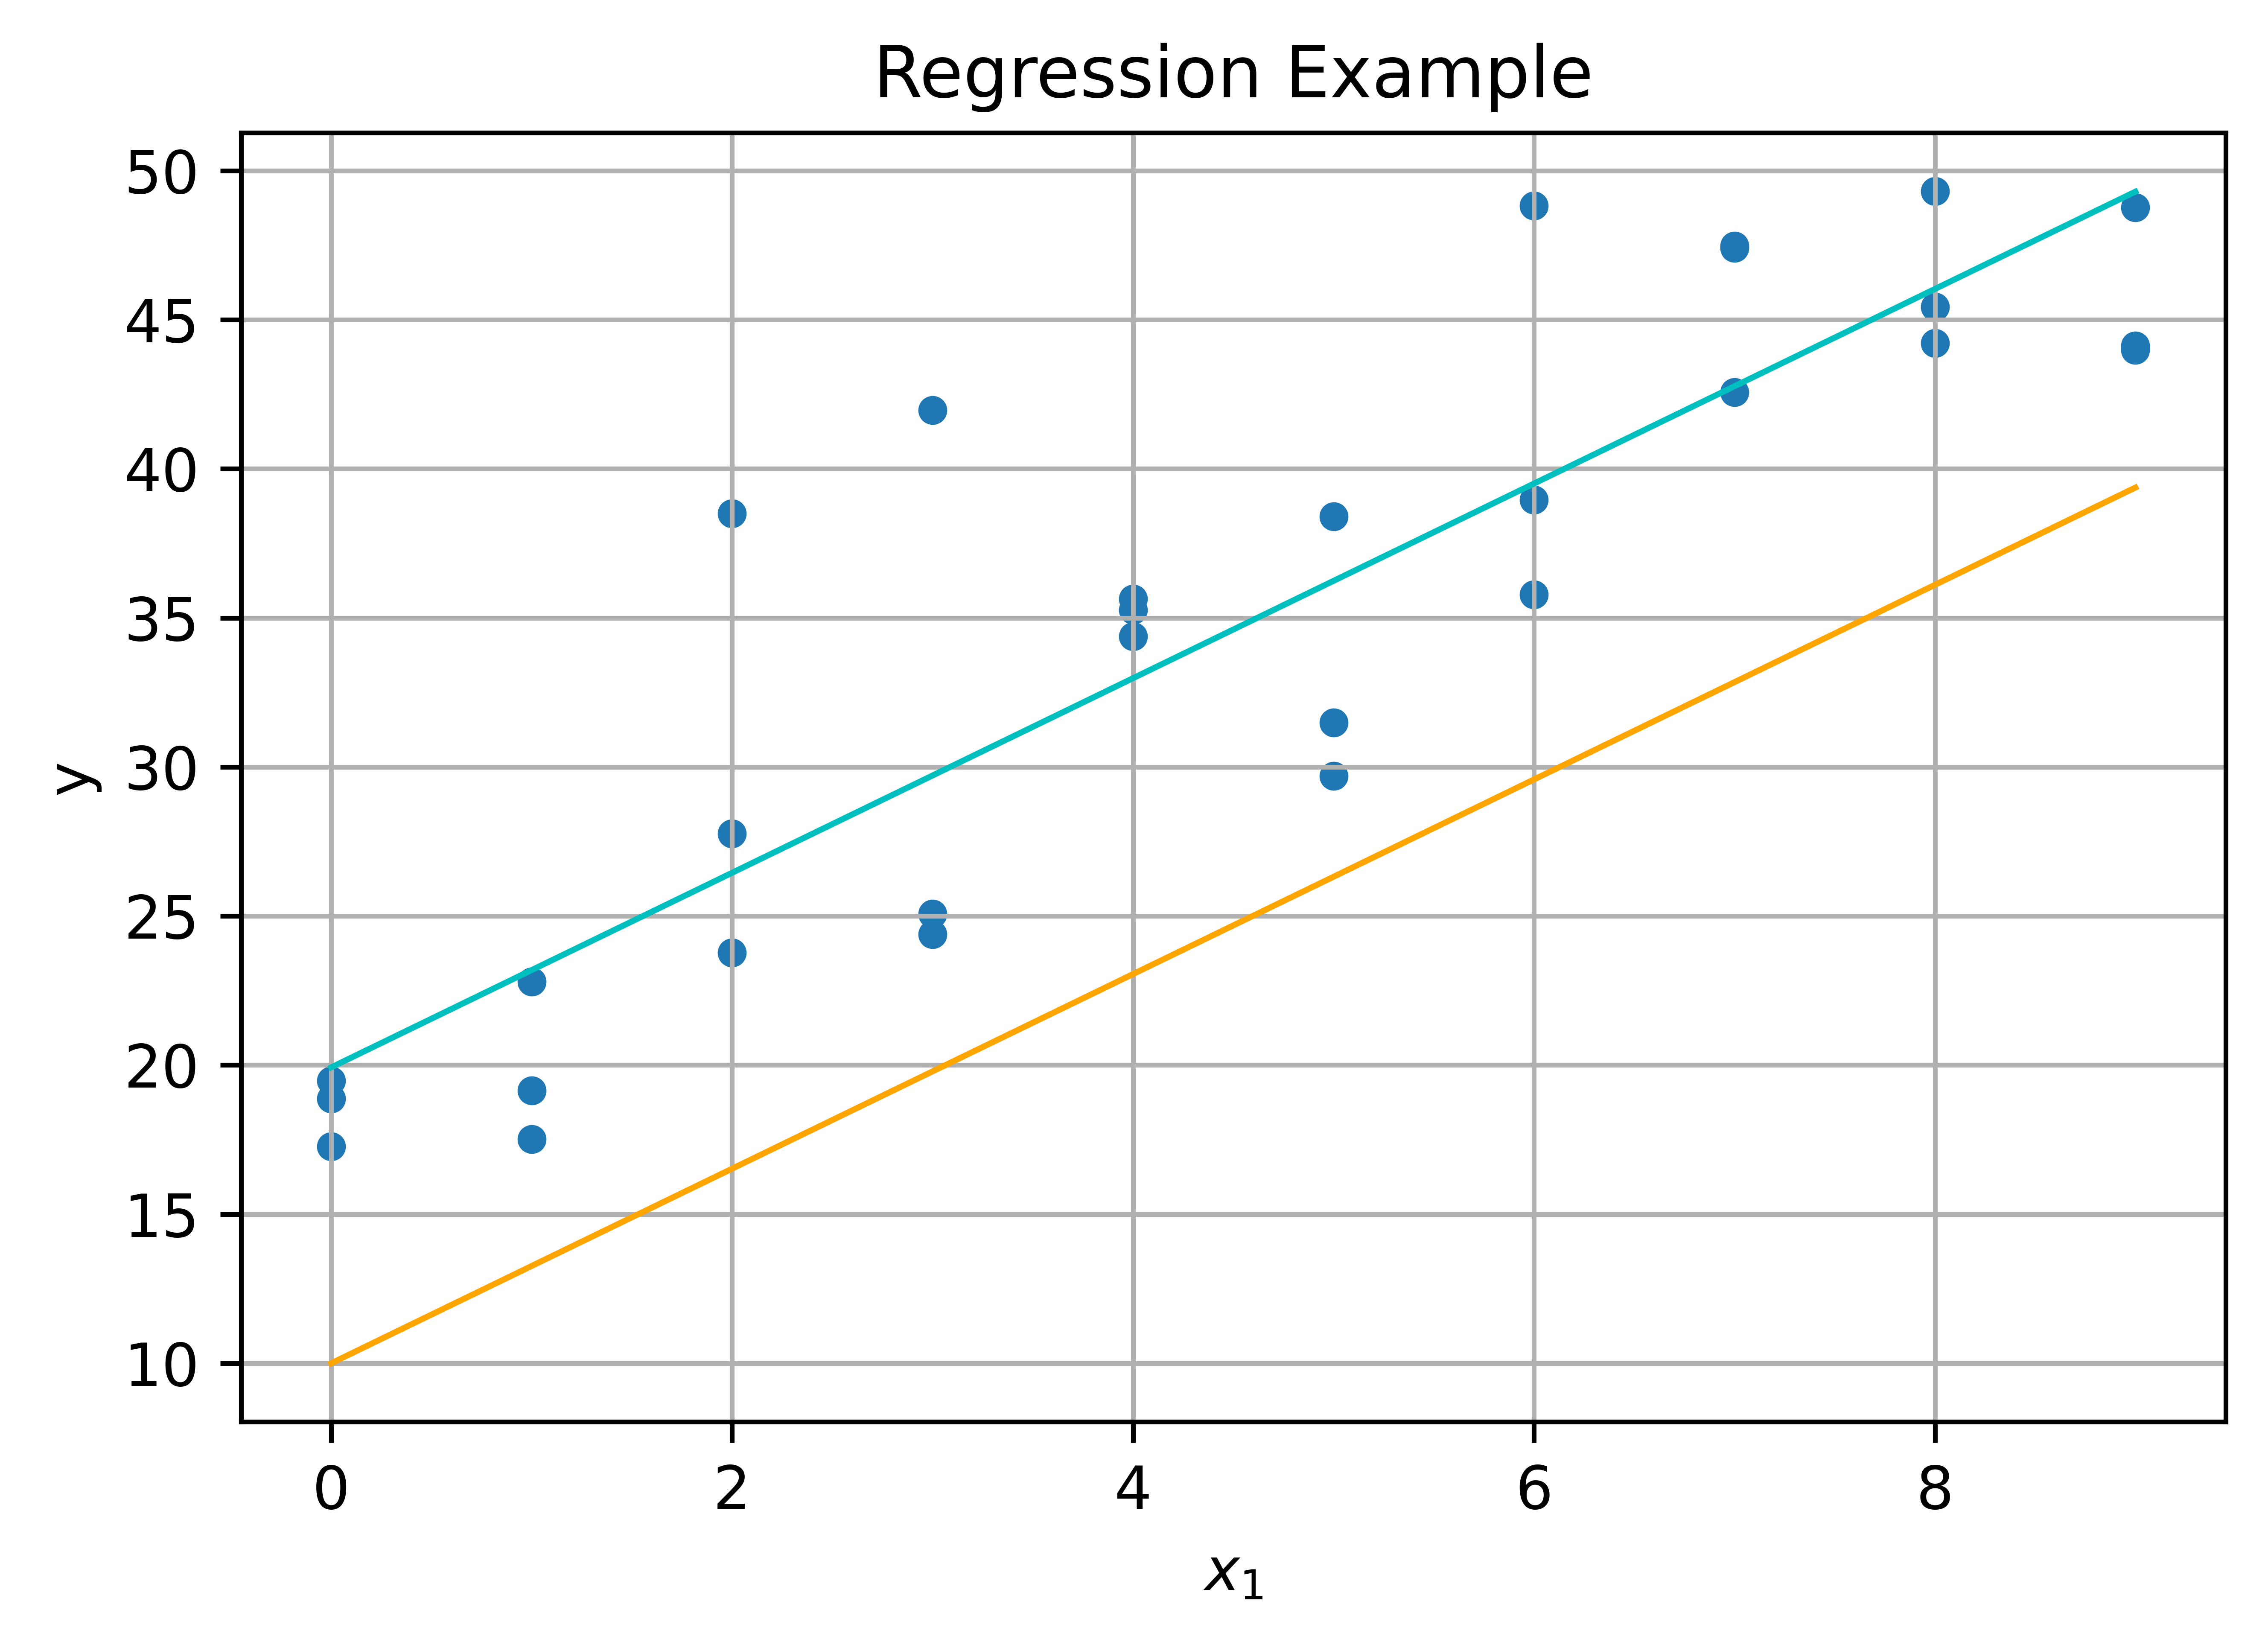
\includegraphics[width=70mm,scale=0.5]{images/regression_images/Regression_Remove_Offset.png}
        
            \caption*{Reducing our offset pulls our line further away from all of our data! This is a serious problem.}
        \end{figure}
        
        This shows that we \textbf{need} our offset! 
        
        \begin{itemize}
            \item We use it to \purp{shift} our hyperplane around the space: otherwise, otherwise, it's difficult to fit data \gren{far} from the origin.
                \note{Imagine that we have three data points at $(1, 1001)$, $(2, 1002)$, and $(3, 1003)$.
                
                \phantom{}
                
                It's clear that our data is offset by roughly 1000: we need $\theta_0$ to address this.}\\
        \end{itemize}
        
        \begin{concept}
            $\theta_0$ gives us a baseline for the \gren{size} of our output values.

            \begin{itemize}
                \item If we reduce $\theta_0$, all of our outputs will be reduced equally: they'll be \purp{less accurate.}
            \end{itemize}
        \end{concept}


    \pagebreak

    \subsection{Ridge Regression Solution}

        Now, we have our regression loss function, 

        \begin{equation}
            J(\Theta) = 
                        \frac{1}{n}  \sum_{i=1}^n 
                        \left( 
                            \underbrace{
                                \red{(\theta^T \ex{x}{i}  
                                + \theta_0)}
                            }_{guess}
                            - \underbrace{
                                \blu{\ex{y}{i}} 
                            }_{answer}
                        \right)^2 
                        + 
                        \underbrace{
                            \pur{ \lambda \norm{\theta}^2 }
                        }_{Regularizer}
        \end{equation}

        Which we can express in matrix form:
            \note{We're gonna cheat a bit, and ignore $\theta_0$.

            \phantom{}
            
            One way to do this is to subtract a constant from every value in $Y$, so that the data is centered on $y=0$: you don't \textit{need} an offset $\theta_0$.

            \phantom{}
            
            But in some problems, we might just include $\theta_0$ in $\theta$, to make our problem simpler, even though we're accidentally regularizing $\theta_0$.}

        \begin{equation}
            J(\theta) = \frac{1}{n}
                    \Big( \red{ \theta^T X - Y } \Big)
                    \Big( \red{  \theta^T X - Y } \Big)^T
            + 
            \pur{\lambda \theta^T \theta}
        \end{equation}

        We can now \gren{optimize} this for $\theta$. We'll do some matrix calculus, omitting the steps here:

        \begin{equation}
            \nabla_{\theta}J = 
            \frac{2}{n}
                    \red{ \Xt^T }
                    \Big( \blu{  \Xt \theta - \Yt } \Big)
            + 
            \pur{2\lambda \theta} = 0
        \end{equation}

        Finally, we \orgg{solve} (using some linear algebra -- multiplying by inverses, distributive property, add/subtracting, etc.):\\

        \begin{kequation}
            The \purp{solution} to the \vocab{ridge regression} problem allows us to find the \gren{optimal} model $\theta^*$.

            \begin{equation*}
                \theta^* = \Big ( \red{\Xt^T \Xt} + \blu{n \lambda I} \Big)^{-1} \org{\Xt^T \Yt}
            \end{equation*}

            or, in our original notation:

            \begin{equation*}
                \theta^* = \Big ( \red{X X^T} + \blu{n \lambda I} \Big)^{-1} \org{XY^T}
            \end{equation*}

            Where $I$ is the $(d \times d)$ identity matrix.
        \end{kequation}

            \note{Review: an identity matrix is a square matrix with 1's on its diagonal, and 0's everywhere else. 
            
            \phantom{}
            
            In general, $AI=IA=A$.}


    \pagebreak

    \subsection{Invertibility}

        This solution is great! We just have one problem:

        \begin{itemize}
            \item It requires that our \purp{inverse} of $(XX^T+n\lambda I)^{-1}$ exists.
        \end{itemize}

        Thankfully, this is true so long as $\lambda>0$!\\

        \begin{concept}
            If $\lambda>0$, we can be sure that $(XX^T+n\lambda I)$ has an \purp{inverse}.

            \begin{itemize}
                \item And thus, we have a \gren{unique solution} to $\theta$ for our \vocab{ridge regression problem.}
            \end{itemize}
        \end{concept}

        You \redd{do not need to know} the linear algebra that justifies this statement. You just need to know that it's true.
            \note{The short version of the justification is:

            \phantom{}
            
            $XX^T$ is positive semi-definite: $v^T XX^T v \geq 0$. 

            \phantom{}
            
            If you add positive elements on the diagonal ($A=XX^T+n \lambda I$), then you can only increase $v^T A v$: now it's $v^T A v > 0$.

            \phantom{}

            Thus, $(XX^T+n\lambda I)$ is positive definite: this means it has an inverse.

            \phantom{}

            If that doesn't make any sense, don't worry about it.}

        This, by the way, presents one more justification for regularization:\\

        \begin{concept}
            Another benefit of \vocab{regularization} is that we can \purp{always} find an \gren{analytical solution} for $\theta$.

            \begin{itemize}
                \item $\Big ( \red{\Xt^T \Xt} + \blu{n \lambda I} \Big)$ is invertible, thus, we can compute 

                \begin{equation*}
                    \theta^* = \Big ( \red{X X^T} + \blu{n \lambda I} \Big)^{-1} \org{XY^T}
                \end{equation*}
            \end{itemize}
        \end{concept}

        Sometimes, we call non-invertible matrices \orgg{singular}.\\

        \begin{definition}
            All of the following statements about square matrix $A$ are equivalent:

            \begin{itemize}
                \item $det(A)=0$.
                \item $A$ has \redd{no inverse}.
                \item $A$ is \gren{singular}.
                \item $A$ is \purp{not full rank}.
            \end{itemize}

            
        \end{definition}

        A few more definitions of singular:

        \begin{itemize}
            \item $A$ has at least one eigenvalue of 0.
            \item $A$ has linearly dependent rows and columns.
            \item $Ax=0$ has a solution other than $x=0$.
                \note{Sometimes, you say this as, "$Ax=0$ has a non-trivial solution".}
            \item $A$ is positive definite.
        \end{itemize}

    \phantom{}

    \subsection{Uniqueness of $\theta^*$}

        This seems suspicious: why on earth would \redd{regularizing} $\theta$ allow us to find a solution?

        \begin{itemize}
            \item In order to understand this, we need to understand \gren{what happens} when $XX^T$ is \purp{singular}.
        \end{itemize}

        \phantom{}

        If $XX^T$ isn't full rank, that means that $X$ \purp{isn't full rank}, either.
            \note{Showing that this is true is more a linear algebra problem than an ML problem, so we'll defer it here.}


        What does this mean? Let's consider an example in 1d: we'll compare a "full rank" version, to one that isn't full-rank.

        \begin{figure}[H]
        \centering
            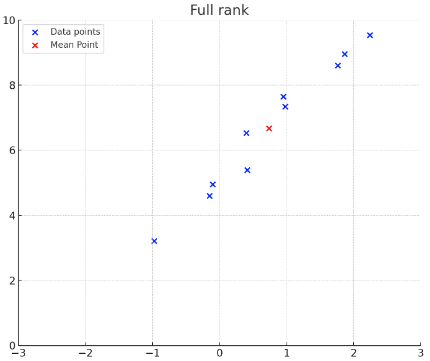
\includegraphics[width=70mm,scale=0.5]{images/regression_images/full_rank.png}
            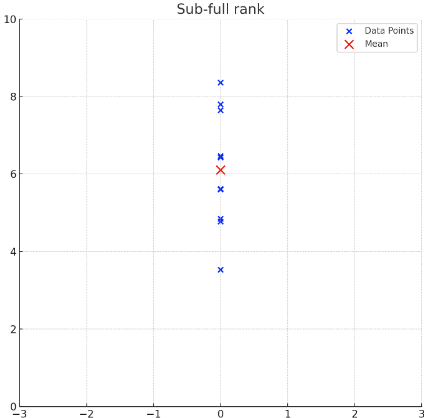
\includegraphics[width=60mm,scale=0.5]{images/regression_images/sub_full_rank.png}
            \caption*{Typically (left plot), we expect our data to be \gren{full rank}: our input space is 1-D, our input data occupies  1-D.

            \phantom{}
            
            But sometimes (right plot), we might have data which is \purp{less than full rank}: in this case, the input data is 0-D: only occupying $x=0$.}
        \end{figure}

        Sure, this data looks weird, but why is this problematic? Because it creates \orgg{multiple optimal solutions}:

        \begin{figure}[H]
        \centering
            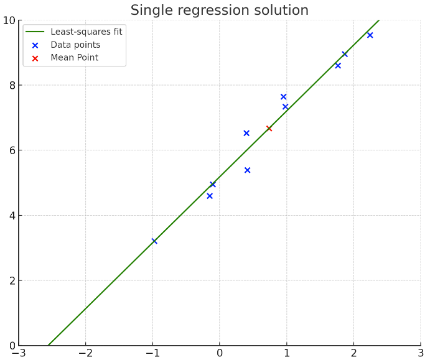
\includegraphics[width=70mm,scale=0.5]{images/regression_images/full_rank_regression.png}
            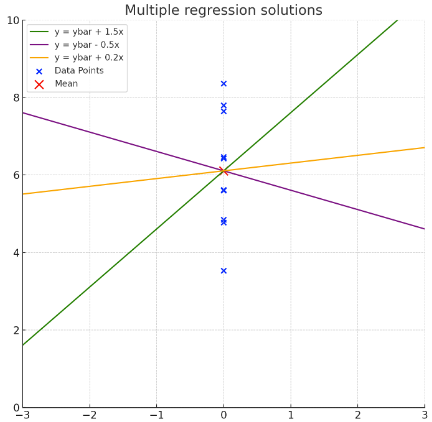
\includegraphics[width=60mm,scale=0.5]{images/regression_images/sub_full_rank_regression.png}
            \caption*{Our "full rank" (left plot) data has one optimal solution.
            
            Our "sub-full rank" (right plot) data has many!}
        \end{figure}

        This is the real reason why, if $XX^T$ isn't invertible, we can't find an analytical solution: there are actually \purp{many} possible solutions!\\

        \begin{concept}
            If $XX^T$ isn't invertible, we \purp{cannot} use our formula to find an analytical (formula-based) \gren{solution} for $\theta$.

            \begin{itemize}
                \item That's because there are \orgg{many optimal solutions}.

                \item In fact, there are \gren{infinitely many of them!}
            \end{itemize}
        \end{concept}

            \note{We call this kind of problem \purp{collinearity}: our input data sit on a lower-dimensional "linear" surface.}

        We can see this in higher dimensions too: below, we have a 2-d input space (3-d plot), but our inputs only occupy a \purp{line}.

        \begin{figure}[H]
        \centering
            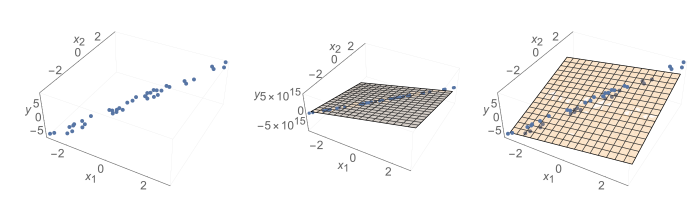
\includegraphics[width=120mm,scale=0.5]{images/regression_images/Regularizer_Multiple_Solutions.png}
        
            \caption*{There are many possible planes that go through that line: each of these is an \gren{equally good} solution for regression.}
        \end{figure}

        \phantom{}

        We don't have this problem if we use regularization: among all of our \gren{equivalent} options, we just pick the one with the \purp{minimal} $||\theta||$.

        \begin{figure}[H]
        \centering
            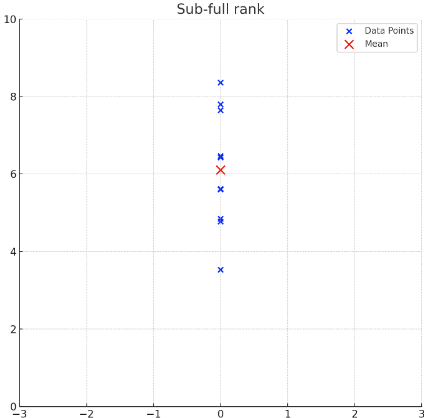
\includegraphics[width=60mm,scale=0.5]{images/regression_images/sub_full_rank.png}
            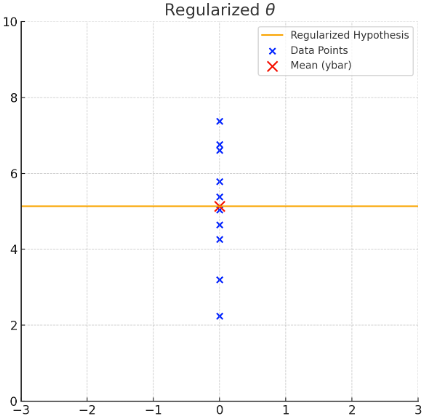
\includegraphics[width=60mm,scale=0.5]{images/regression_images/singular_data_regularized.png}
            \caption*{Now, we have one solution: we can get this analytically!}
        \end{figure}
            

        \pagebreak

    \subsection{Error Amplification}

        Surely, this is a really rare situation: our data typically won't line up \gren{perfectly}.

        \begin{itemize}
            \item Maybe, but that's part of the problem: let's see what happens if our data is \purp{not} perfectly aligned. We say that $XX^T$ is \vocab{ill-conditioned} or "nearly singular".\\
        \end{itemize}

        \begin{definition}
            We call a matrix \vocab{ill-conditioned} or \purp{nearly singular} if it is very close to a singular/non-invertible matrix.
        \end{definition}

            \note{You can compute whether a matrix is ill-conditioned using something called a "condition number", but we'll omit that point.}

        \begin{figure}[H]
        \centering
            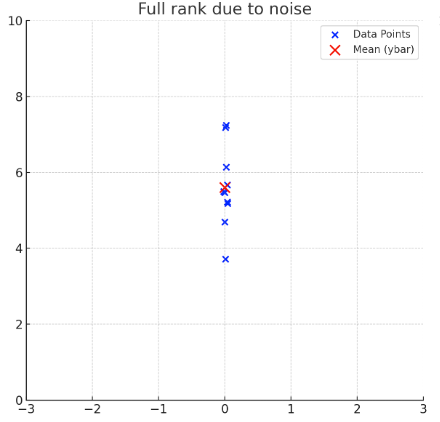
\includegraphics[width=60mm,scale=0.5]{images/regression_images/noisy_full_rank.png}
            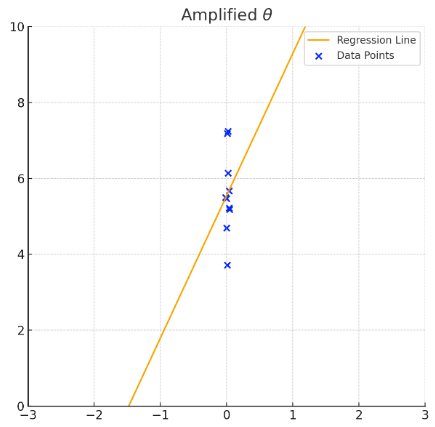
\includegraphics[width=60mm,scale=0.5]{images/regression_images/amplified_theta.png}
            \caption*{Our data has a \gren{large slope} now! This is a problem: $x$ has \purp{no effect} on $y$, we just added a little noise to the $x$-axis.}
        \end{figure}

        Our model notices, "\gren{very small} change in $x$, \purp{moderate} change in $y$", and assumes the slope $\theta$ should be \orgg{large}.
            \note{Another way to see this: technically, if you wanted to draw a line through the data, you'd draw a vertical line: "infinite" slope.}

            \begin{itemize}
                \item This is wrong: our change in $y$ isn't actually explained by $x$, it's explained by some "\purp{randomness}" in the output (which is common in real data).\\
            \end{itemize}

        \begin{concept}
            One problem with data that \textit{almost} falls on a line, is \vocab{error amplification}.

            \begin{itemize}
                \item If $x_i$ varies by a small amount, while $y$ varies by a larger amount, our model may assume $\theta_i$ is \purp{very large}.

                \item That means that, if you had a much larger $x_i$ value, the model will predict $y$ is \orgg{way larger}.
            \end{itemize}

            Thus, our error gets \purp{amplified} as we move further away.
        \end{concept}

            \note{Sometimes, you might hear people mention "numerical instability" of the inverse when a matrix has a small determinant: these are, mathematically, the same problem.
            
            \phantom{}
            
            If $det(A)=0.01$, then $det(A^{-1})=100$. The closer you are 0, the more dramatic the effect.}


        If our problem is that $\theta$ is too large, then we can solve this problem by regularizing $\theta$.

        \begin{figure}[H]
        \centering
            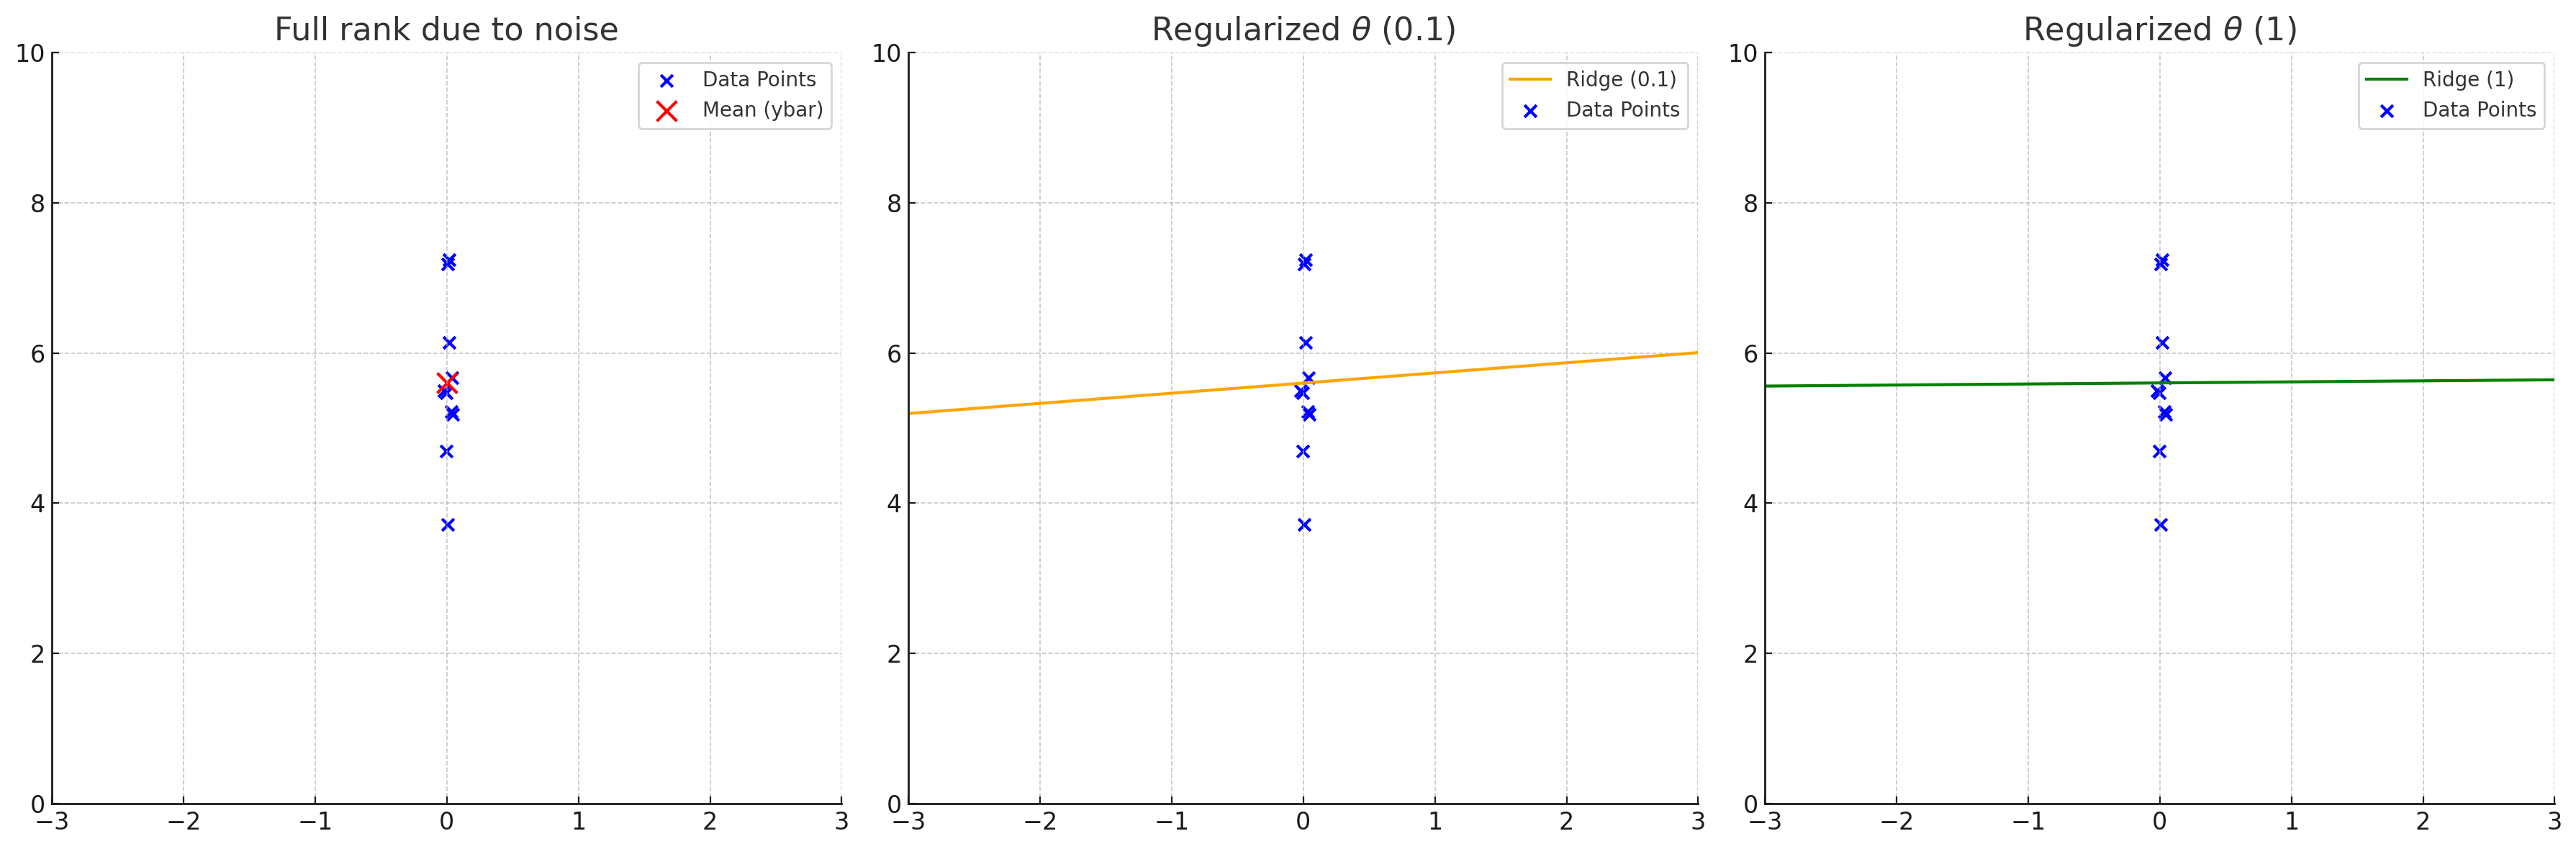
\includegraphics[width=150mm,scale=0.5]{images/regression_images/full_rank_noise_regularized.png}
            \caption*{With $\lambda=0.1$, our slope is already much less sharp. with $\lambda=1$, we end up with (mostly) the same solution as we did in the singular case.}
        \end{figure}

        \begin{concept}
            \vocab{Ridge Regression} helps \purp{improve} our model by
            
            \begin{itemize}
                \item Making our model more \purp{general} and resistant to \gren{overfitting}
                \item Making sure \gren{solutions} are \purp{unique}
                \item Keeping our matrix $XX^T$ \purp{invertible}, so we can find a \gren{solution}.
            \end{itemize}
        \end{concept}

        \phantom{}

        \subsection{Error Amplification Example (\redd{Optional})}

            Here's a very simple computational example:

            \begin{itemize}
                \item \miniex Suppose that two inputs are \orgg{almost exactly the same}: $x_1^{(1)}=0$, and $x_1^{(2)}=0.01$. 
                \item But, the outputs are \purp{somewhat} different.  The outputs are $y^{(1)}=25$, $y^{(2)}=26$.
            \end{itemize}

            If we assume \textbf{all} of the change in the output is a result of the the \textbf{input}, then it looks like a \gren{tiny} change in $x_1$ has a \purp{huge} effect on the output $y$.

            \begin{equation}
                \deriv{y}{x} = \frac{\Delta y}{\Delta x} = \frac{1}{.01} = 100
            \end{equation}
    
            This suggests that $x_1$ has a \redd{100x} effect on our output! Even though, it could just be that $x$ has small variation, and $y$ has larger variation.
    
            \begin{equation}
                100 x_1 + 25 = h(x)
            \end{equation}

            Imagine that $x_1=10$: suddenly, the prediction is 1025. That's why we call it \vocab{error amplification}: a small error near $x=0$, becomes huge as we get further away.


    

    \pagebreak
    \subsection{Regularizer justification: Prior Knowledge (\redd{Optional})}

        One more way to justify our regularizer applies to a lot of broader statistics: the concept of a \vocab{prior belief}.

        \begin{itemize}
            \item Suppose we have prior expectations about what our model should look like: based on theory, or prior experience.

            \item We might consider a model \textbf{more different} from that past one, $\Theta_{\text{prior}}$, to be \textbf{suspicious}, and less likely to be good.
        \end{itemize}

        So, we can \purp{punish our model} for being too different from that expectation.

        \begin{itemize}
            \item This makes our model more \gren{conservative}: it avoids creating a very "extreme" model, without strong justification from the training data.
                \note{Our data has to "convince" us that it's worth trying a different model.}\\ 
        \end{itemize}
       
        \begin{concept}
            If we have a \purp{prior} hypothesis $\Theta_{\text{prior}}$ to work with, we might improve our \purp{new} model by encouraging it to be \gren{closer} to the old one.
            
            \begin{equation*}
                R(\Theta)= \norm{ \Theta - \Theta_{\text{prior}} }^2
            \end{equation*}
            
            We measure how \gren{similar} they are using \vocab{square distance}.
            
        \end{concept}
        
        \miniex You have a \textbf{pretty good} model for \textbf{predicting} company profits, but it isn't perfect. You decide to train a \textbf{better} one, but you expect it to be \textbf{similar} to your old one.

        \phantom{}

        In our case, we \purp{don't have} a prior hypothesis $\theta_{prior}$. We have no clue of what a \gren{good solution} looks like.

        We'll take a neutral stance:

        \begin{itemize}
            \item When we know nothing, we're \orgg{equally likely} to expect $\theta_k$ to be positive, or negative. 
            \item In other words, we don't know if $x_i$ is likely to increase or decrease $y$.
        \end{itemize}

        So, our guess should average out to 0: the most likely effect is \purp{none}.

        \begin{itemize}
            \item Another way to justify this: if we pick a bunch of variables randomly, we might expect a lot of them to be \orgg{irrelevant}.
            \item \miniex Without knowing anything, we probably don't expect your birth date to affect your academic performance, positive or negatively.
        \end{itemize}

        Thus, we treat $\Theta_{\text{prior}} = \vec{0}$.\\

        \begin{concept}
            We can interpret \vocab{ridge regression} as expecting each $\theta_k$ terms to be close to 0.
            
            \begin{itemize}
                \item In other words, $\Theta_{\text{prior}}=\vec{0}$.
            \end{itemize}

            \begin{equation*}
                R(\Theta) = ||\theta-\vec{0}||^2 = ||\theta||^2 
            \end{equation*}

            This is the same formula we arrived at earlier.
        \end{concept}
        
    
\pagebreak
%%%%%%%%%%%%%%%%%%%%%%%%%%%%%%%%%%%%%%%%%%%%%%%%%%%%%%%%%%%%%%%%%%%%%%%%%%%%%%%%%%%%%%%%%%%
        
\section{Evaluating Learning Algorithms}

    Now, we have successfully developed an \textbf{algorithm} for \textbf{learning} from our data. But, did our algorithm make a \textbf{good} hypothesis? How do we do \textbf{better}?
    
    \subsection{What $\lambda$ should we choose?}
    
        There's something we ignored earlier: how do we pick the \textbf{best} value of $\lambda$? We didn't go into detail, but that value of $\lambda$ will affect our algorithm's \textbf{performance}.
        
        \begin{itemize}
            \item We mentioned that different $\lambda$ values have different \textbf{tradeoffs}, so we need to figure out which $\lambda$ value is best for our problem.
            
            \item This $\lambda$ adjusts exactly how we learn: how do we balance learning from \textbf{data} against the need to \textbf{generalize}?
        \end{itemize}
        
        So, we need to \textbf{optimize} our $\lambda$ value. Let's figure out how to go about that.
        
    \subsection{Tradeoffs: Estimation Error}
    
        High and low $\lambda$ values have benefits and drawbacks. These tradeoffs can be loosely divided into \textbf{two categories}.
        
        When we generalize, we're trying to avoid \vocab{estimation error}: we incorrectly guess the overall distribution we're trying to fit. We \textbf{estimate} poorly if we \textbf{generalize} poorly.\\
        
        \begin{definition}
            \vocab{Estimation error} is the error that results from poorly \gren{estimating} the \purp{solution} we're trying to find. 
            
            This can be caused by \gren{overfitting}, getting a bad (\purp{unrepresentative}) sample, or not having enough \gren{data} to come to conclusion.
        \end{definition}
        
        \miniex Let's try a regression problem, but we'll use only 4 points to make our plot.
        
        \begin{figure}[H]

            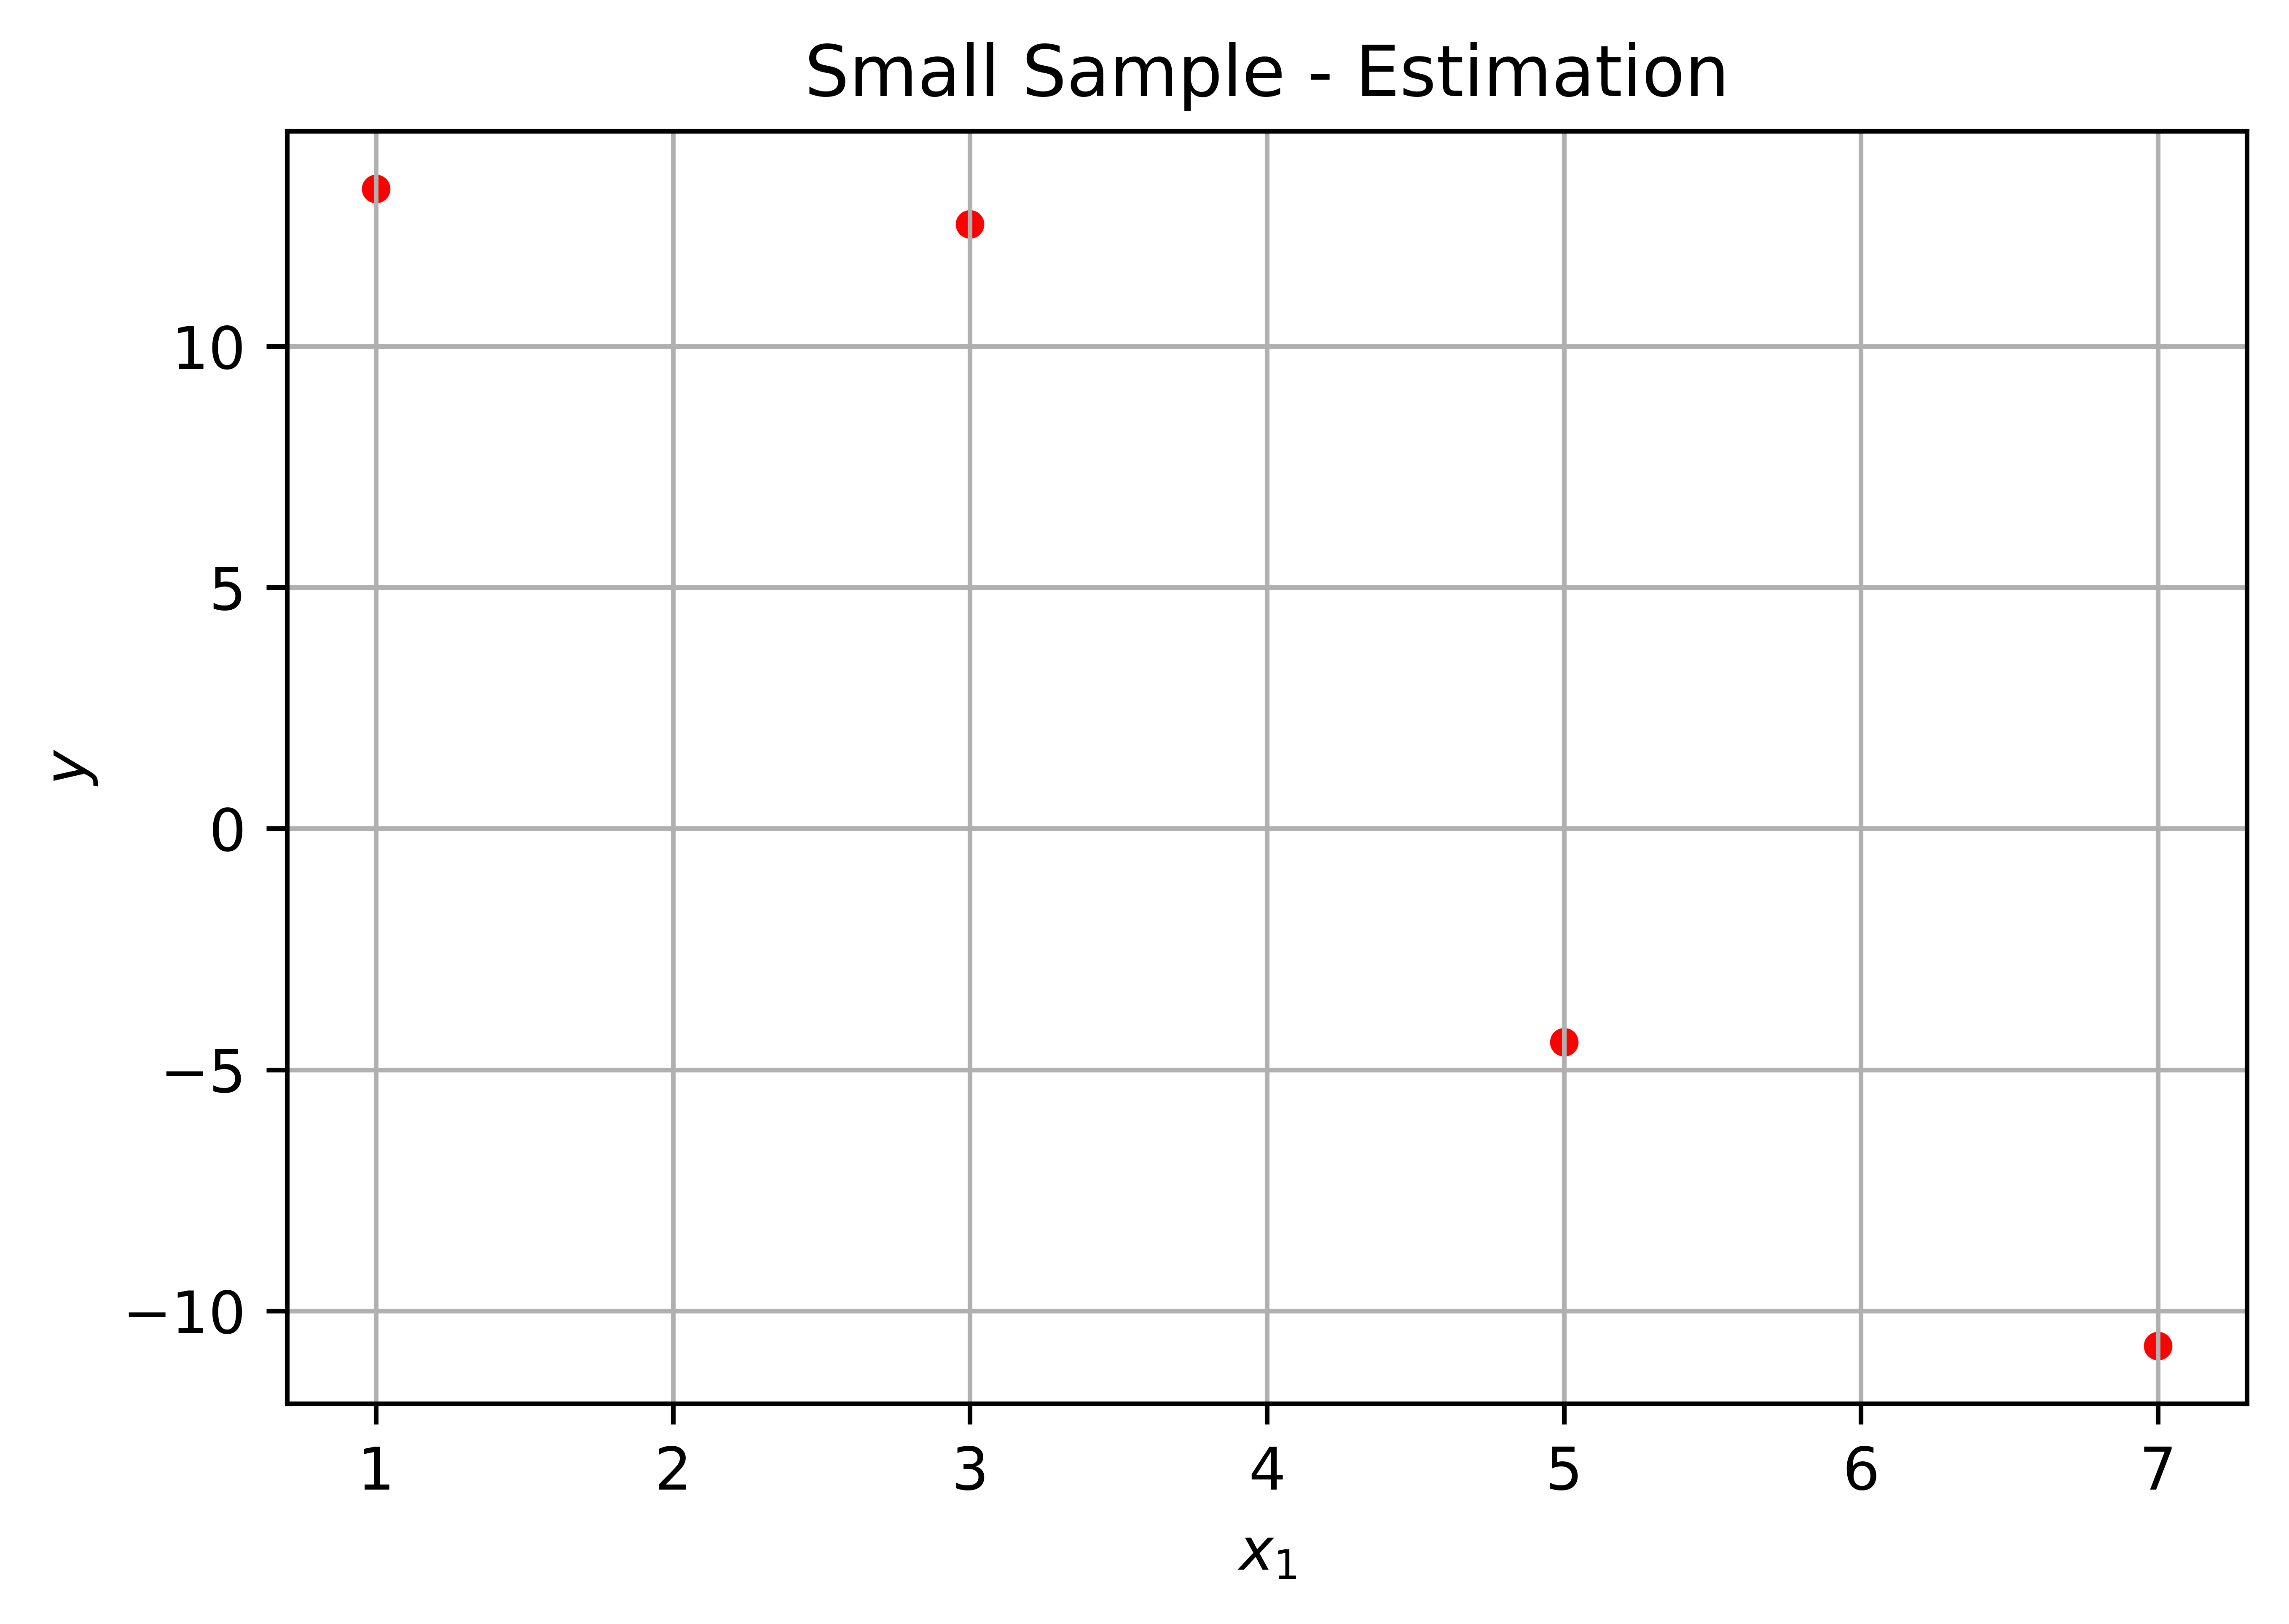
\includegraphics[width=70mm,scale=0.5]{images/regression_images/Estimation_Limited_Sample.png}

            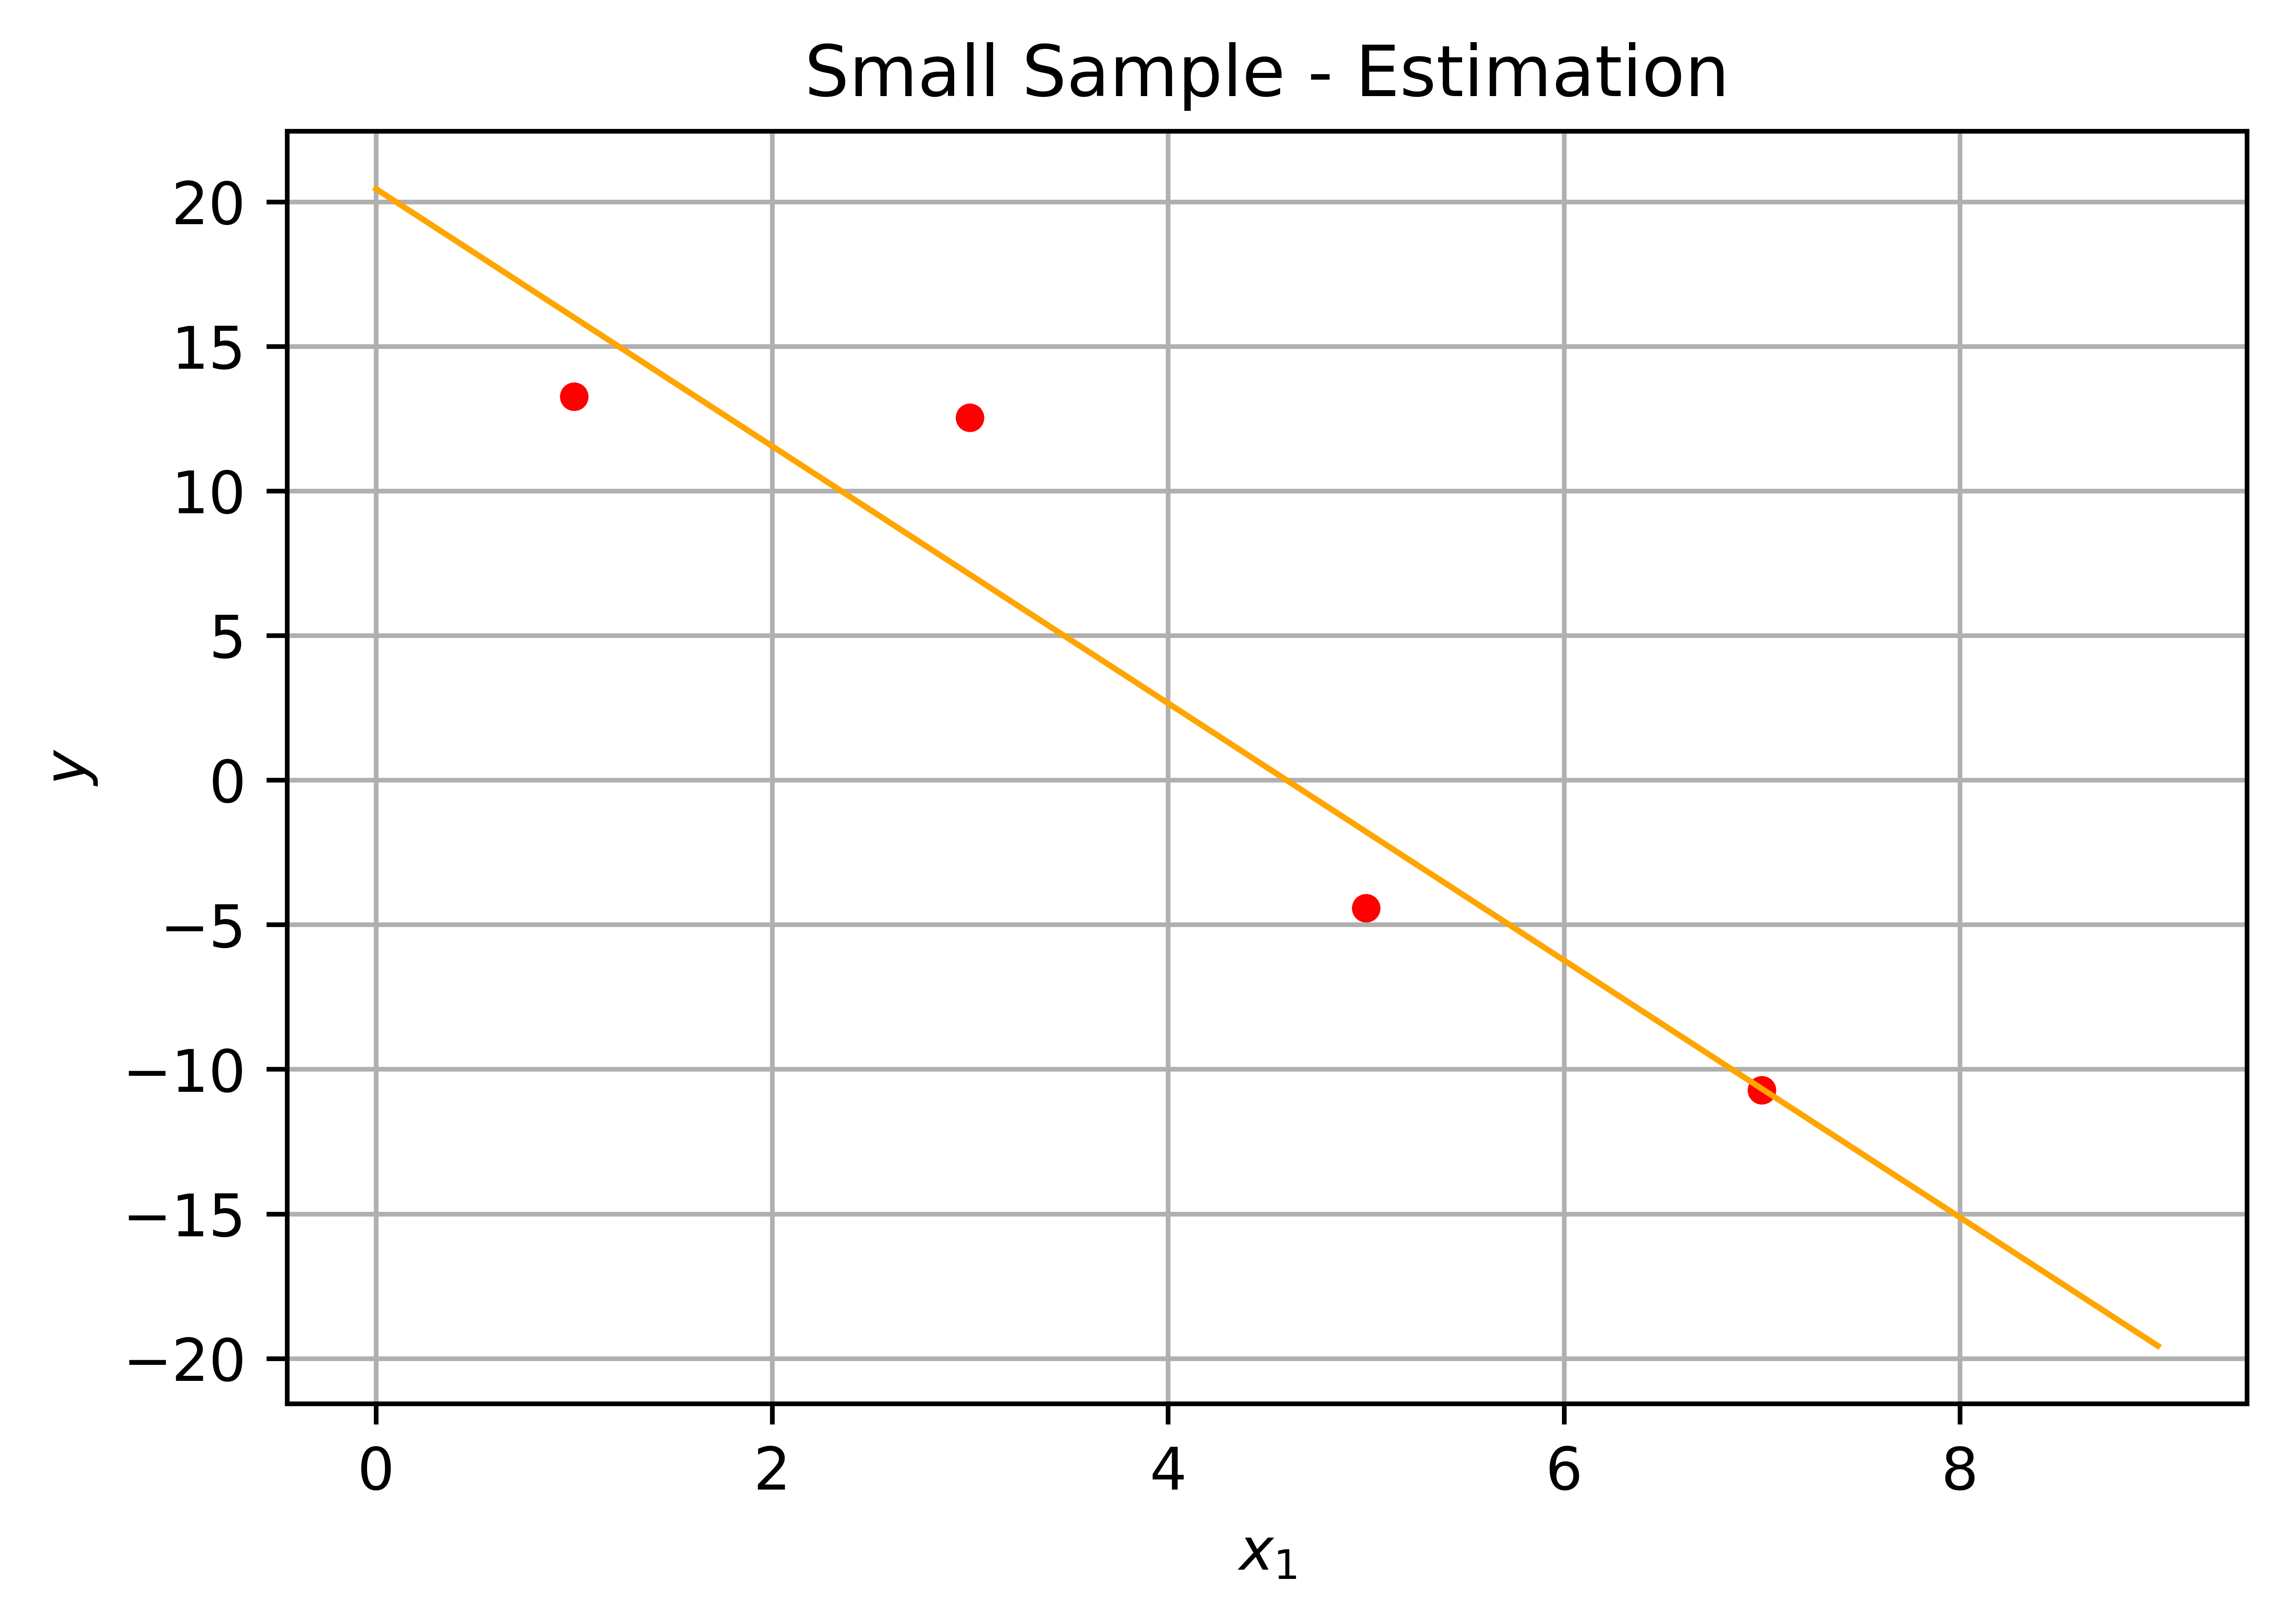
\includegraphics[width=70mm,scale=0.5]{images/regression_images/Estimation_Limited_Sample_Regression.png}
        
            \caption*{This is the regression solution we get based on our small dataset.}
        \end{figure}
        
        We might be suspicious. One way to reduce \textbf{estimation error} is to increase our number of data points (though this isn't always an option, or sufficient!)
        
        \begin{figure}[H]

                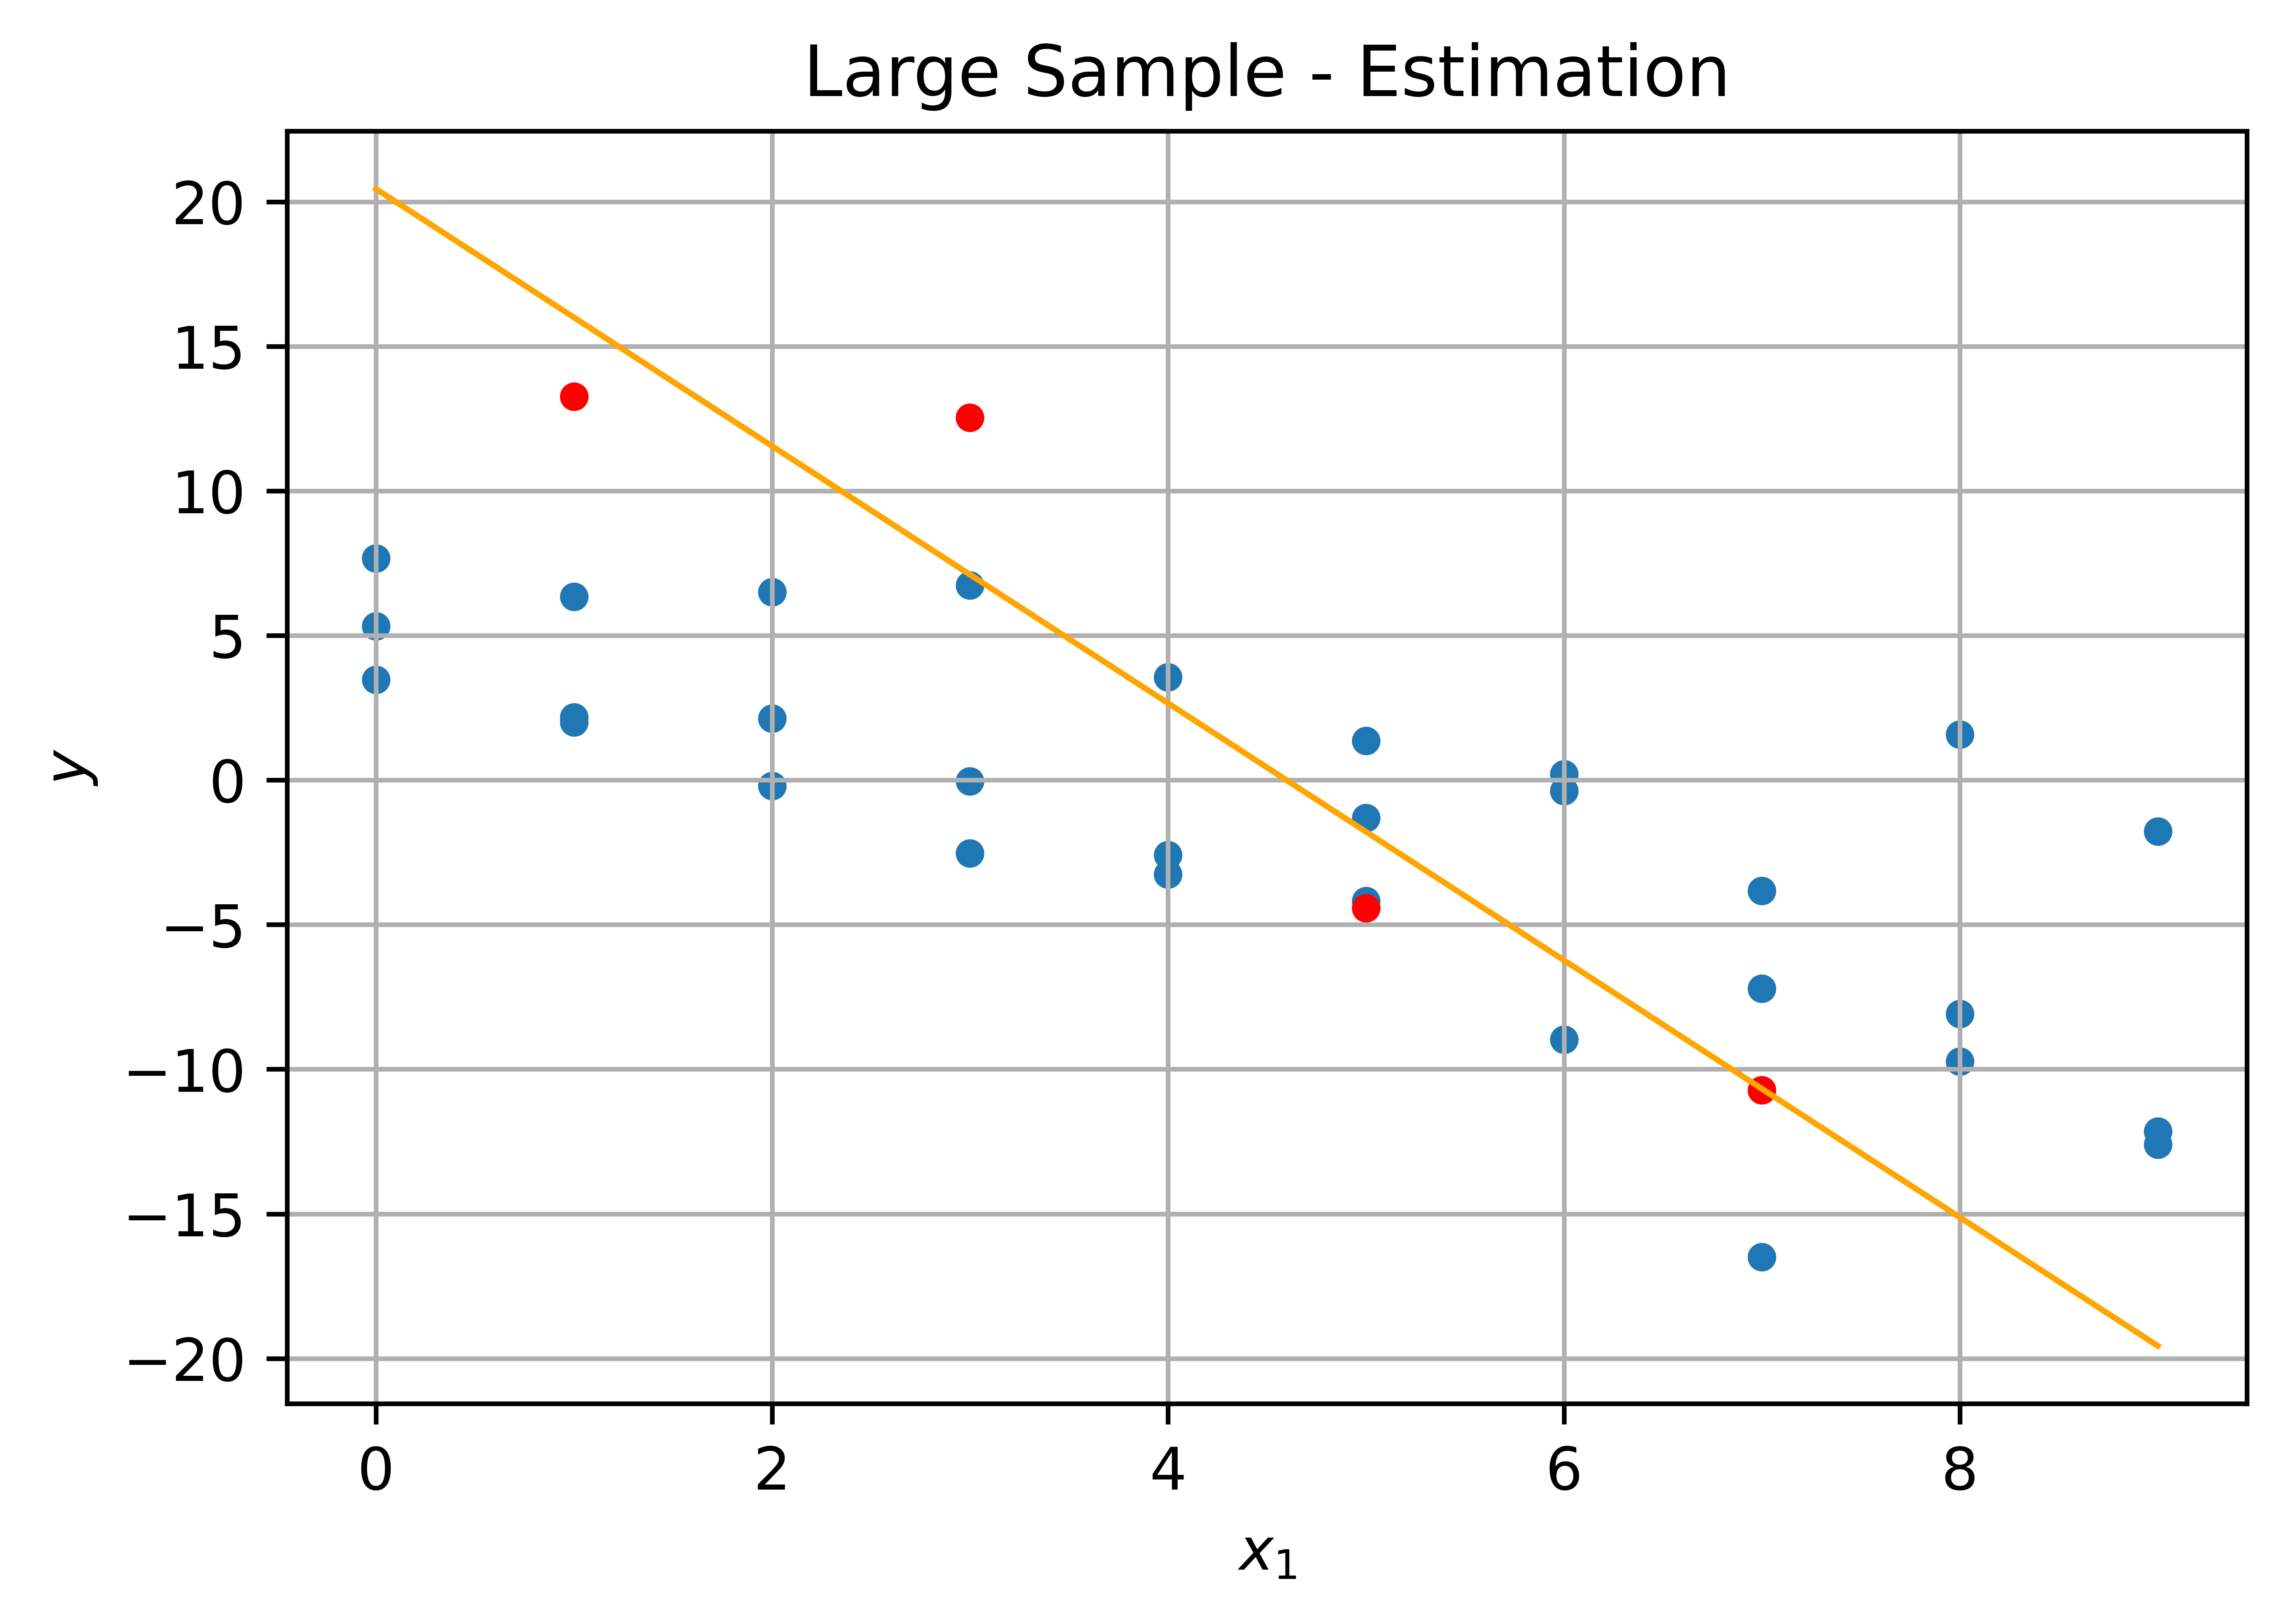
\includegraphics[width=70mm,scale=0.5]{images/regression_images/Estimation_Full_Sample.png}
                
                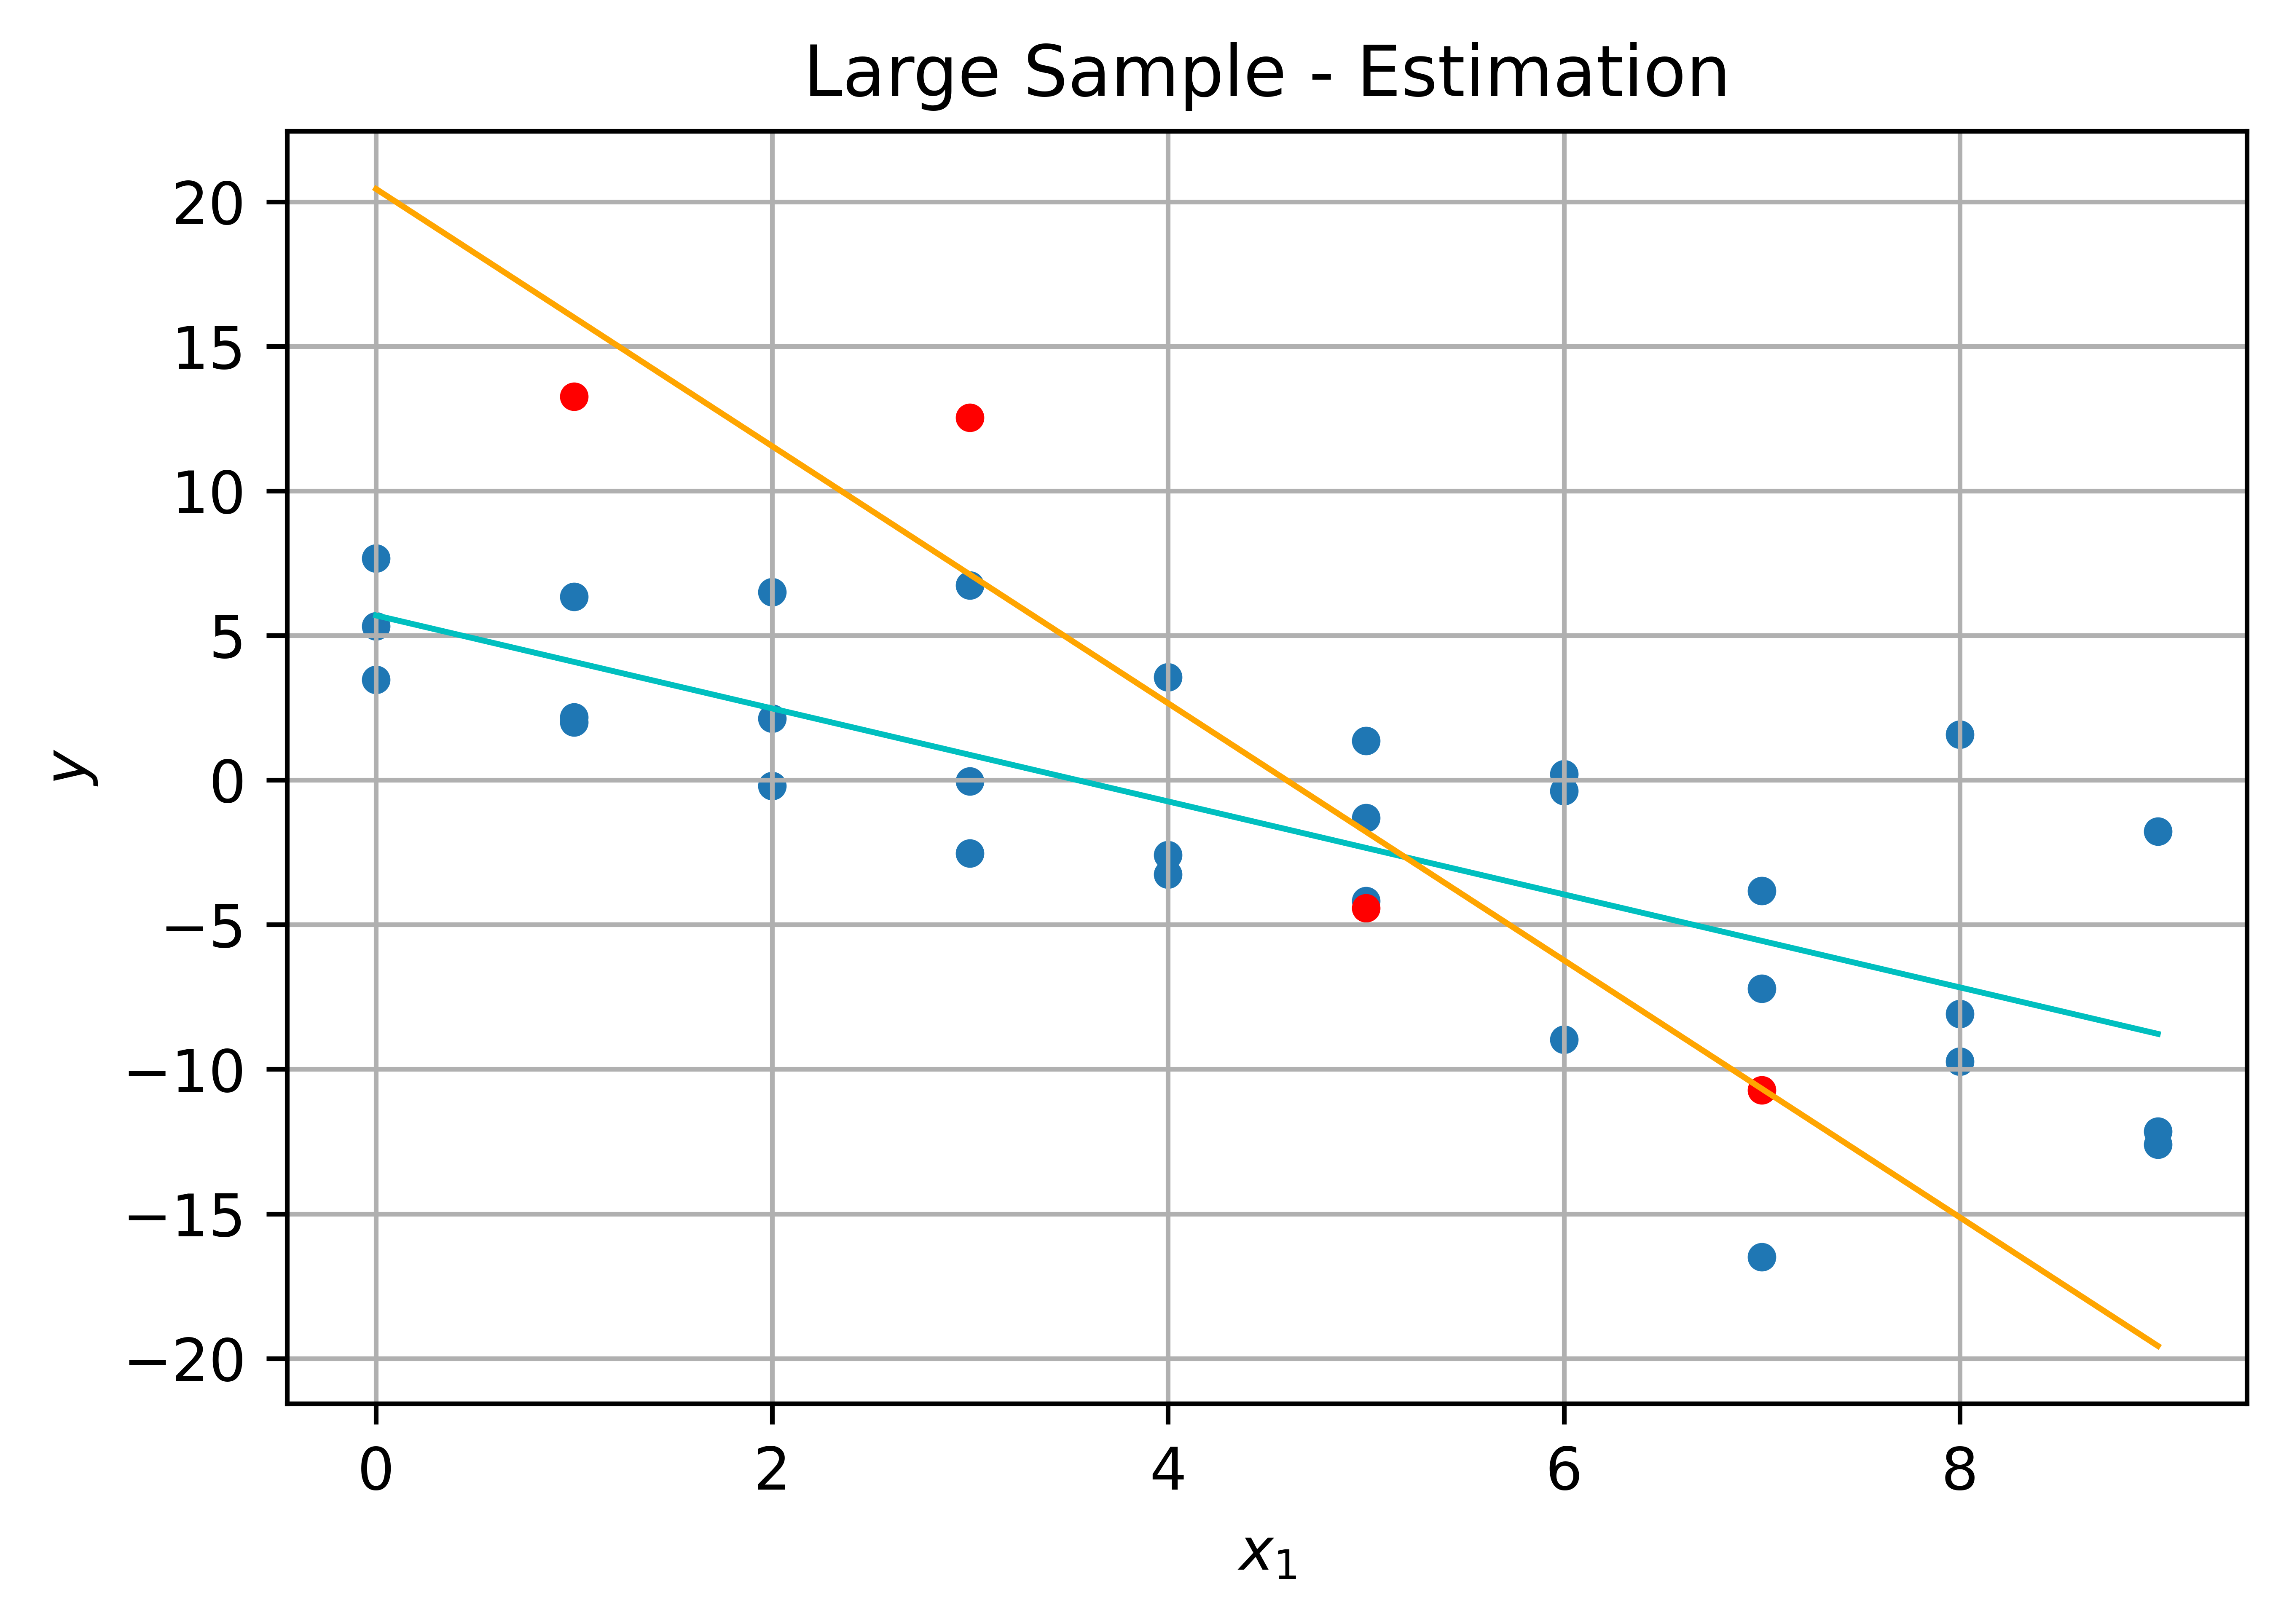
\includegraphics[width=70mm,scale=0.5]{images/regression_images/Estimation_Full_Sample_Regression.png}
        
            \caption*{Our regression from before doesn't look so good on this model... We make an updated regression, and get a more accurate result.}
        \end{figure}
        
        \begin{clarification}
           $\lambda$ doesn't lower \purp{estimation error} in the \gren{same way} that increasing \purp{sample size} does, but the problem is \gren{similar}.
        \end{clarification}
        
    \subsection{Tradeoffs: Structural Error}
    
        However, not all problems are caused by estimation error: sometimes, it \textbf{isn't even possible} to get a good result - you chose the wrong \textbf{model class}.
        
        This means the \textbf{structure} of your model is the problem, not your method of \textbf{estimation}. Thus, we call this \vocab{structural error}.\\
        
        \begin{definition}
            \vocab{Structural error} is the error that results from having the wrong \gren{structure} for the \purp{task} you are trying to accomplish.
            
            This can result from the \gren{wrong class} of model, but sometimes, your model class doesn't have the \purp{expressiveness} it needs for a complex problem.
            
            It can also happen if your algorithm \purp{limits} the available models in some way, like how $\lambda$ does.
        \end{definition}
        
        \miniex If the \textbf{true shape} of a distribution is a parabola $x^2$, there is \textbf{no} linear function $mx+b$ that can match that: this creates \textbf{structural error}.
        
        \begin{figure}[H]
        
                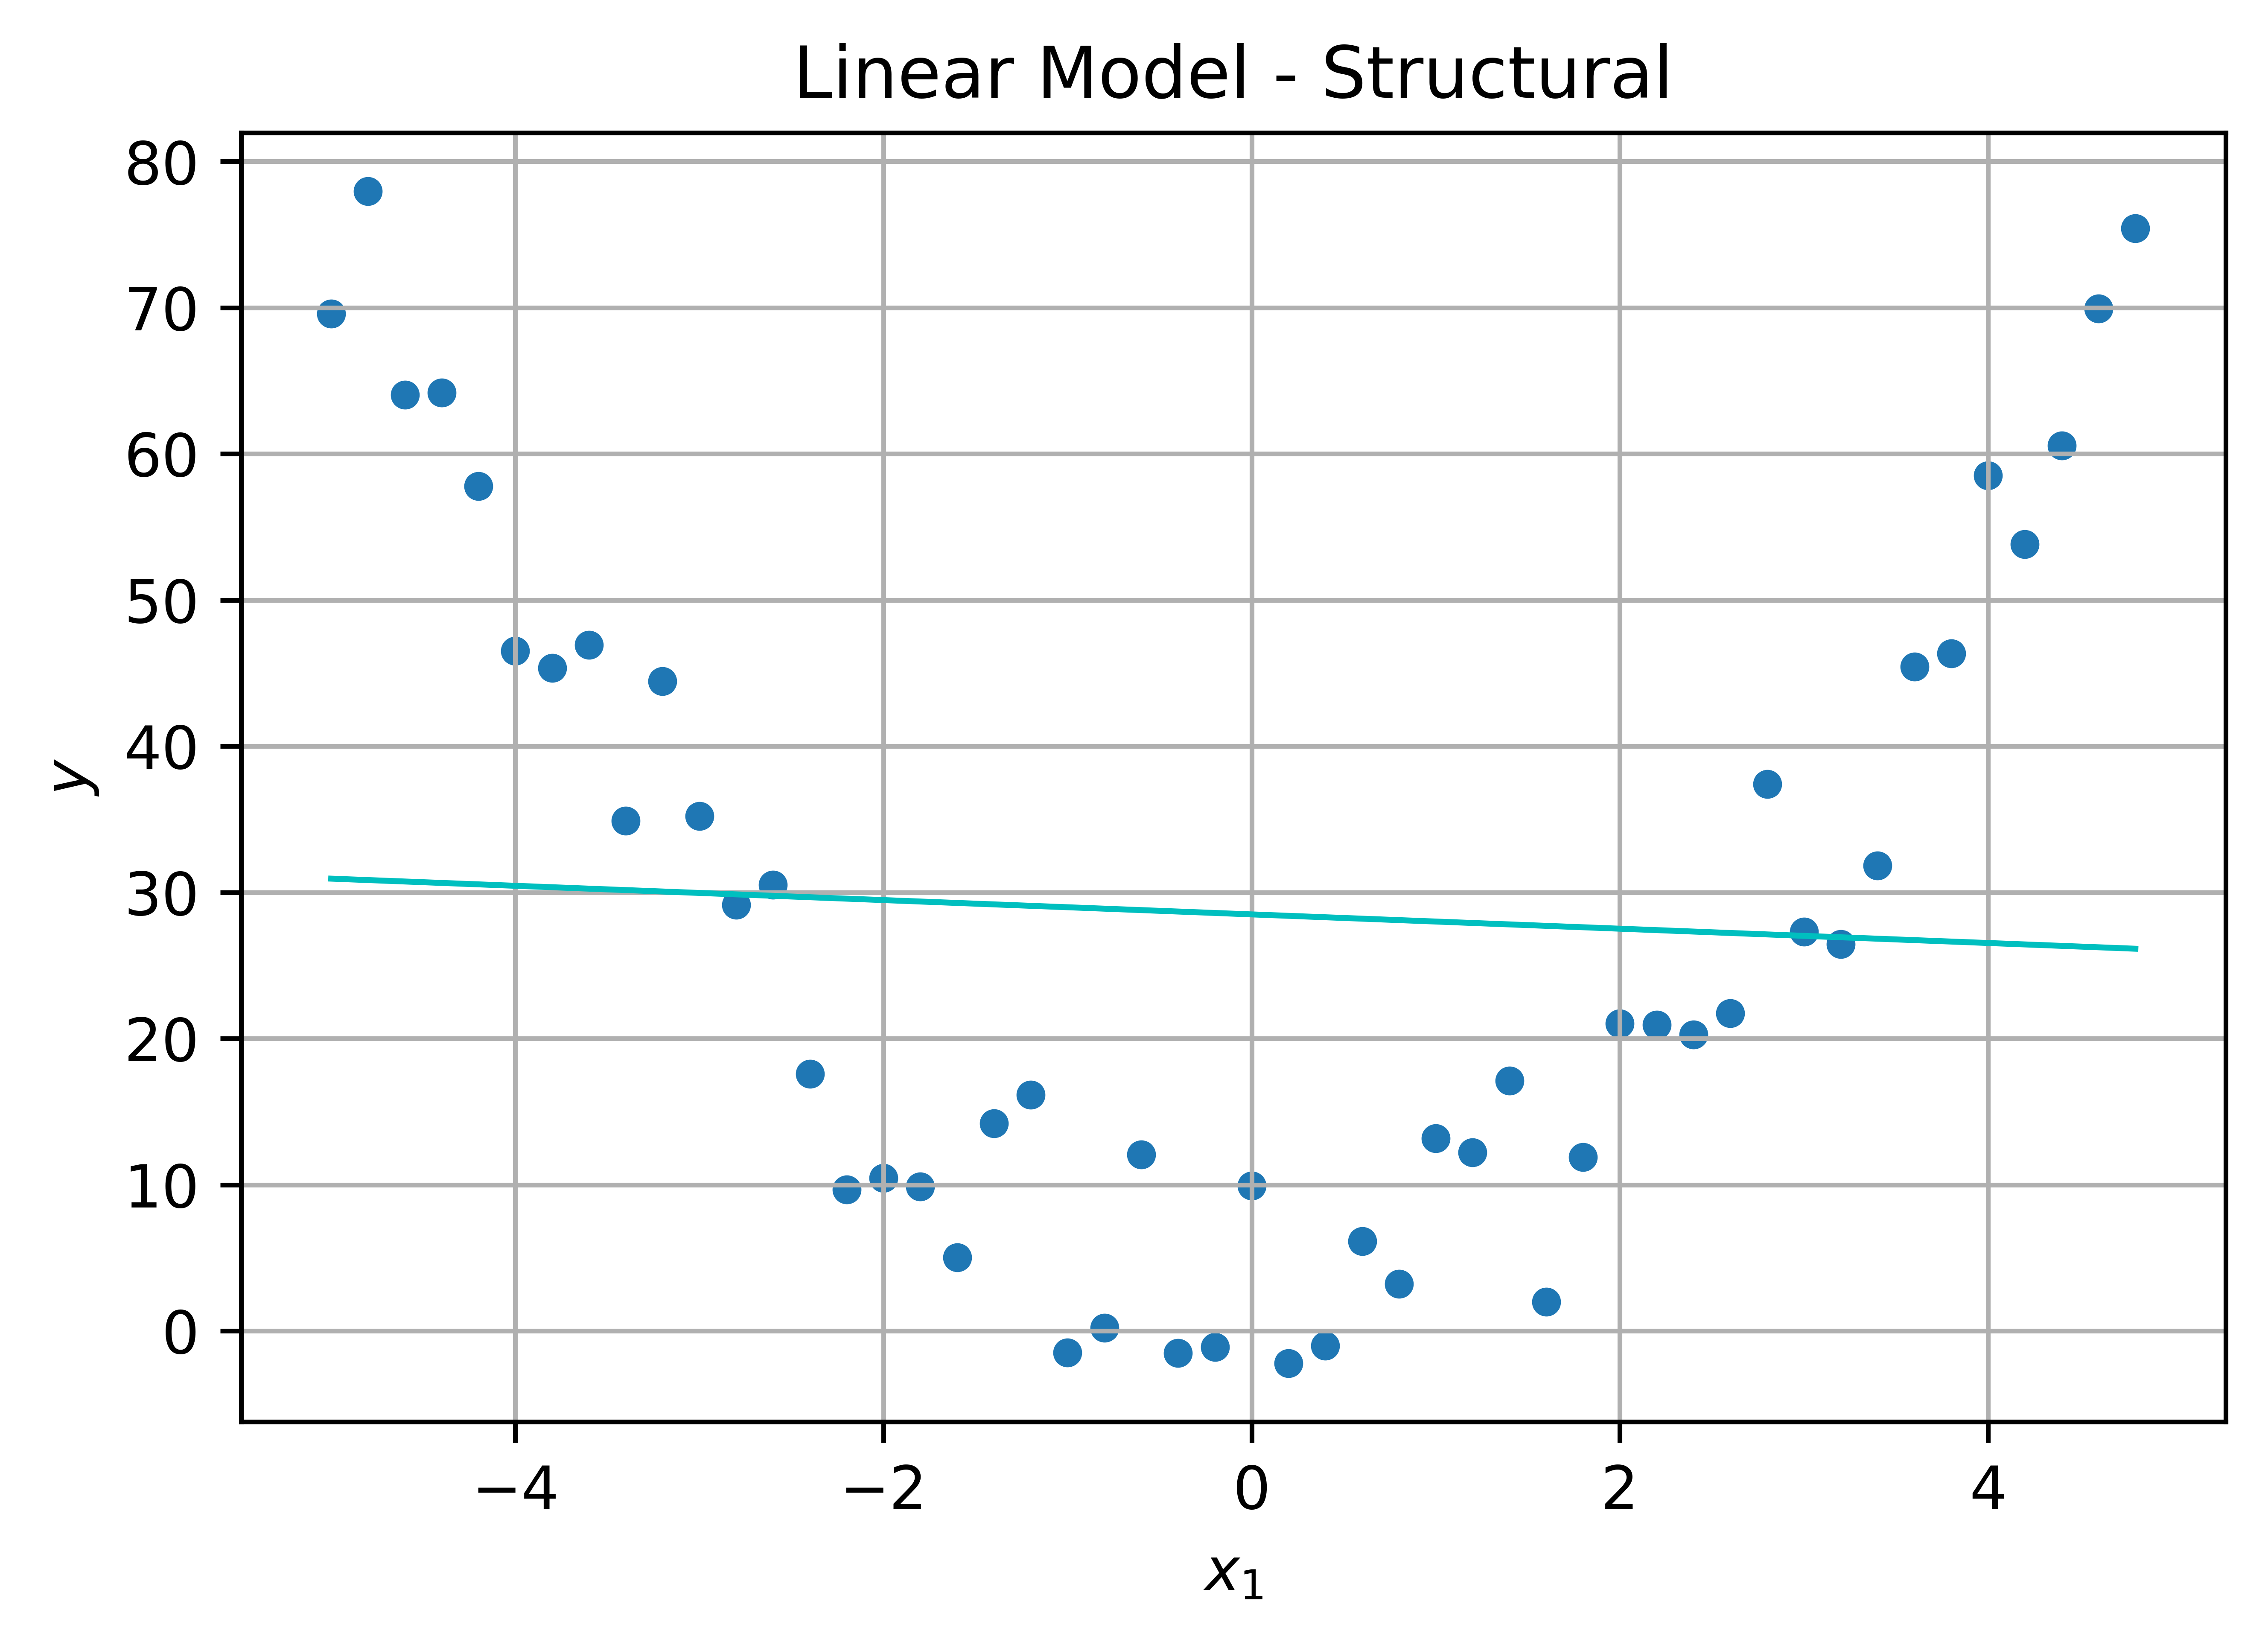
\includegraphics[width=70mm,scale=0.5]{images/regression_images/Structural_Linear_Model.png}

                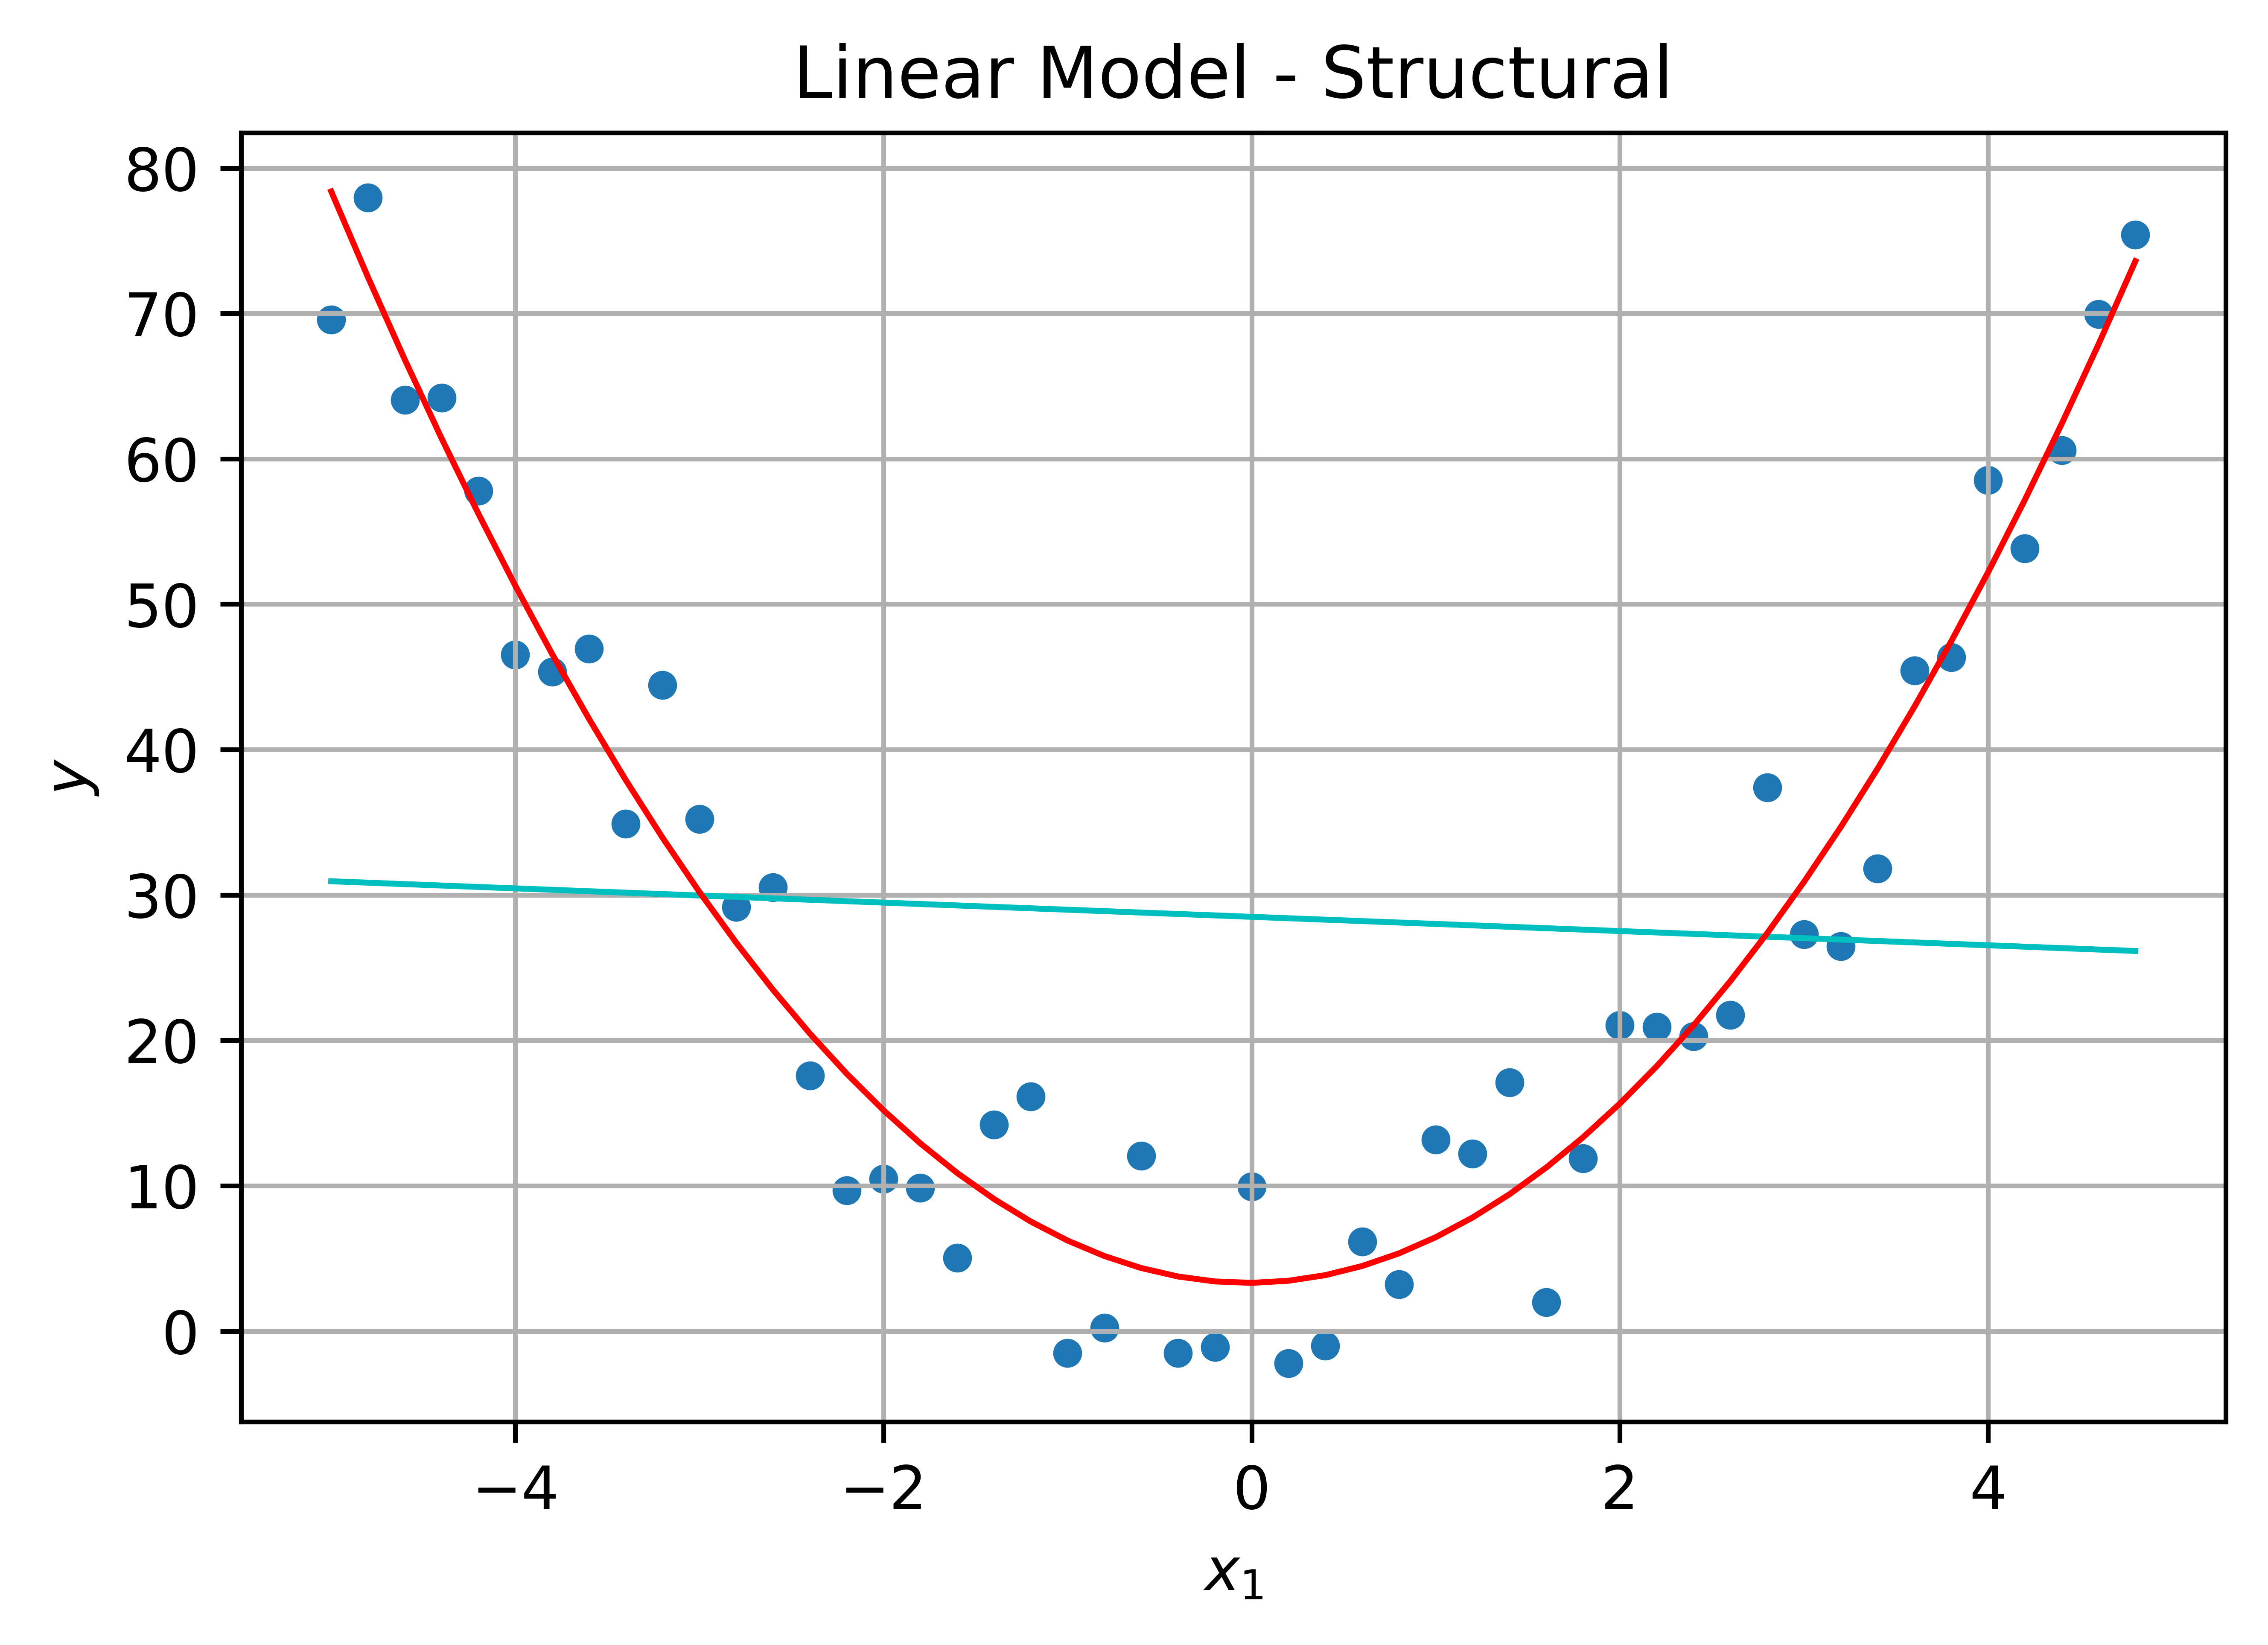
\includegraphics[width=70mm,scale=0.5]{images/regression_images/Structural_Quad_Model.png}

        
            \caption*{Our \textbf{linear} model isn't able to represent a quadratic function... so, we switch to a more \textbf{expressive} model: a \textbf{quadratic} equation.}
        \end{figure}
        
        \note{Remember that \textbf{expressiveness} is about how many possible models you have: if you have more models, you can solve more problems.}
        
        \begin{clarification}
           Note that $\lambda$ does not restrict our model class \purp{as severely} as \gren{switching polynomial order}, like above. 
        
            But, $\lambda$ \purp{limits} the use of larger $\theta$, which does make it \gren{unable} to solve some problems. So, the \purp{structural error} problem is similar.
        \end{clarification}
        
    \subsection{Tradeoffs of $\lambda$}
        
        Based on these two categories, we can discuss the tradeoffs of $\lambda$ more easily.
        
        As we mentioned, regularization \textbf{reduces} estimation error: 
        
        If we overfit to our current data, we are poorly \textbf{estimating} the distribution, because the training data may not perfectly \textbf{represent} it.\\
        
        \begin{concept}
            A \vocab{large $\lambda$} means \purp{more regularization}: we more strongly push for a more \gren{general} model, over a more \gren{specific} one.
            
            This results in...
            
            \begin{itemize}
                \item \gren{Reduced} estimation error
                \item \purp{Increased} structural error
            \end{itemize}
        \end{concept}
        
        However, \textbf{regularization} also \textbf{limits} the possible models we can use - those it views as less "general", it \textbf{penalizes}.

        \begin{itemize}
            \item That means the scope of possible models is \textbf{smaller} - some models are no longer \textbf{acceptable}. What if the only valid solution was in that space we \textbf{restricted}? Well, then we can't \textbf{find} it.
            
            \item That means there are certain \textbf{structural} limits on our model: that means that regularization \textbf{increases} structural error!\\
        \end{itemize}
        
        
        
        
        
        \begin{concept}
            A \vocab{small $\lambda$} means \purp{less regularization}: we care less about a more \gren{general} model, allowing more \gren{specific} data to come into play.
            
            This results in...
            
            \begin{itemize}
                \item \purp{Increased} estimation error
                \item  \gren{Reduced} structural error
            \end{itemize}
        \end{concept}
        
    \subsection{Evaluating Hypotheses}
    
        So, we know that we have these \textbf{two} types of \textbf{error}. But it's \textbf{difficult} to \textbf{measure} them separately. 
        
        So instead, we just want to measure the \textbf{overall performance} of our hypothesis. 
        
        We do this using our \textbf{testing error}: this tells us how good our hypothesis is \textbf{after} training.
        
        \begin{equation}
            \testerr(h) =
            \frac{1}{m}  
            \sum_{i\purp{=n+1}}^{\purp{n+m}} 
                \left( 
                    h(\ex{x}{i}) - \ex{y}{i} 
                \right)^2
        \end{equation}
        
        Note that, before, we were using \textbf{regularization}. This is so we can \textbf{make} a more \textbf{general} model. 
        
        But here, we've \textbf{removed} it, because training is \textbf{done}: we're \textbf{not} going to make our hypothesis \textbf{better}. We just care about how \textbf{good} it came out.
        \note{We're already measuring the \textbf{generalizability} by using \textbf{new data}!}\\
        
        \begin{clarification}
            When we \vocab{evaluate a hypothesis} using \purp{testing error}, we are \gren{done training}: our hypothesis will not change.
            
            Because of this, we \orgg{do not} include the \orgg{regularizer} when \gren{evaluating} our hypothesis.
        \end{clarification}
        
    \subsection{$\lambda$'s purpose: learning algorithms}
    
        Notice that we \textbf{removed} regularization when we were \textbf{evaluating} our hypothesis: regularization was used to \textbf{create} our hypothesis, but it is not \textbf{part} of that hypothesis.
        \note{Our hypothesis only includes the parameters $\Theta$: not $\lambda$!}
        
        That's because $\lambda$ is part of our \textbf{algorithm}: it determines how we find our hypothesis. So, let's talk about that.\\
        
        \begin{definition}
            A \vocab{learning algorithm} is our procedure for \purp{learning} from data. It uses that data to create a \gren{hypothesis}. We can diagram this as:
            
            \begin{equation*}
                \data_n \longrightarrow 
                \boxed{\text{learning alg ($\hclass$)}} 
                \longrightarrow h
            \end{equation*}
            
            In a way, it's a function that takes in \gren{data} $\data_n$, and outputs a \purp{hypothesis} $h$.
        \end{definition}
        
        We're choosing \textbf{one hypothesis} $h$ from the hypothesis class $\hclass$: this is why $\hclass$ appears in the notation above.
        \note{We can write this as $h \in \hclass$}
        
    \subsection{Comparing Hypotheses and Learning Algorithms}
        
        We can take our learning algorithm
        
        \begin{equation*}
            \data_n \longrightarrow 
            \boxed{\text{learning alg ($\hclass$)}} 
            \longrightarrow h
        \end{equation*}
        
        And compare it to our hypothesis $h$:
        
        $$ x \rightarrow \boxed{h} \rightarrow y $$
        
        In a way, our learning algorithm is a function, that outputs another function!
        \note{This is similar to $\trainerr$, which instead takes a function as \textbf{output}!}

        \begin{itemize}
            \item Our \gren{hypothesis} can be adjusted with our \purp{parameter} $\Theta$: if we change $\Theta$, we change our \textbf{performance}.
            
            \item Our \gren{learning algorithm} depends on $\lambda$: so, $\lambda$ is like a \purp{parameter}. But, it's different from $\Theta$: $\Theta$ \orgg{is} our model, $\lambda$ controls how we \orgg{choose} our model.
                \begin{itemize}
                    \item So, it's a parameter ($\lambda$) that affects other parameters ($\Theta$). Because of that, we call it a \textbf{hyperparameter}.
                        \note{It affects our hypothesis by pressuring it to have lower magnitude!}\\
                \end{itemize}
        \end{itemize}
        
        
        
        
        
        
        
        \begin{definition}
            \purp{Parameters} are \gren{variables} that adjust the behavior of \purp{our model}: our hypothesis.
            
            A \vocab{hyperparameter} is a \gren{variable} that can adjust \purp{how we make models}: our learning algorithm. 
        \end{definition}
        
        The \textbf{only} hyperparameter we have for now is $\lambda$, but the \textbf{development} of hyperparameters is an ongoing area of \textbf{research}.\\
        
        \begin{concept}
            \vocab{Lambda}, or $\lambda$, is a \vocab{hyperparameter}: it controls our \purp{learning algorithm.}
        \end{concept}
        
    \subsection{Evaluating our Learning Algorithm}
    
        So, while we can evaluate each \textbf{hypothesis}, it's also important to measure how our \textbf{learning algorithm} is performing.
        
        How do we measure it? Well, the job of our \textbf{learning algorithm} is to \textbf{pick good hypotheses}.\\
        
        \begin{concept}
            We can \vocab{evaluate} the performance of a \vocab{learning algorithm} using \orgg{testing loss}: a good learning algorithm will create \gren{hypotheses} with low testing loss.
        \end{concept}
        
        You could think of this as measuring the \textbf{skill} of a \textbf{teacher} (the learning algorithm) by the \textbf{success} of their \textbf{student} (the hypothesis) on a \textbf{test} (testing loss).
        
    \subsection{Validation: Evaluating with lots of data}
    
        When we were creating hypotheses, \purp{randomness} caused some problems: you might not get \textbf{training data} that matched the \textbf{testing data} very well.
        
        The \textbf{same} can happen here, when \textbf{evaluating} your \textbf{algorithm}: maybe your model happened to create a bad (or unusually good!) hypothesis because of \textbf{luck}.
        
        The easy solution to \textbf{randomness} is to add \gren{more data}: we get more \textbf{consistency} that way.
        
        So, we \textbf{repeatedly} get new training data and test data. For each, we train a \orgg{different hypothesis}. We can \textbf{average} their performance out, and use that to \textbf{estimate} the quality of our algorithm.\\
        
        \begin{definition}
            \vocab{Validation} is a way to \vocab{evaluate a learning algorithm} using \vocab{large amounts of data}.
            
            We do this by \gren{running} our algorithm \purp{many times} with new data, and \gren{averaging} the testing error of all the hypotheses.

            \begin{itemize}
                \item This process is often requires having \purp{lots of data} to train with, but is a \textbf{provably} good approach.
            \end{itemize}
            
        \end{definition}
        
    \subsection{Our Problem: When data is less available}
        
        As mentioned, this takes up \textbf{lots of data}. What if our data is limited?
            \note{Data is often \textbf{expensive}. It might even be impossible to get more!}

        In this case, we'll assume that have some \textbf{finite} data, $\data_n$. We \textbf{can't get more}.
        
        Previously, we solved validation by using \textbf{more data}, and generating \gren{multiple hypotheses}.

        \begin{itemize}
            \item One set of data gives us one \textbf{hypothesis}.

            \item But, what if, rather than using \textbf{completely} new data for each hypothesis, we used \orgg{slightly different} data each time?
        \end{itemize}
        
         
        
        First, need to break $\data_n$ into a chunk for training, and a chunk for testing.
        
        \begin{figure}[H]
        \centering
            
\includegraphics[width=70mm,scale=0.5]{images/regression_images/training_and_test_data.png}
        \end{figure}
        
        How do we get more hypotheses from this dataset?
        
    \subsection{Cross-Validation}
    
        We mentioned that we want \textbf{different} hypotheses. Our hypotheses depend on our \textbf{training data}. So we want to \textbf{change} our training data.
        
        We can't \textbf{add} data to it, because then we \textbf{lose} testing data. We shouldn't \textbf{remove} training data, because then we're just making a hypothesis that's \textbf{less well-informed}.
        
        Instead, we'll \textbf{swap} some of the training data for testing data.
        
        \begin{figure}[H]
        \centering
            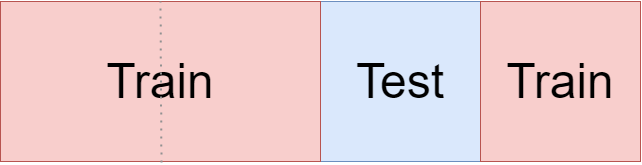
\includegraphics[width=70mm,scale=0.5]{images/regression_images/training_and_test_data_2.png}
        \end{figure}
        
        This will create a new hypothesis, and the data is partially different! In fact, we can do this for each of our chunks:
        
        \begin{figure}[H]
                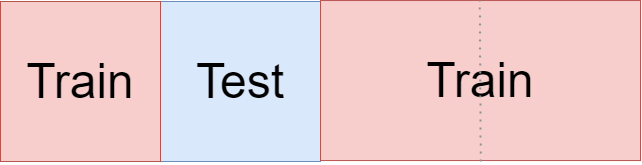
\includegraphics[width=70mm,scale=0.5]{images/regression_images/training_and_test_data_3.png}
                
                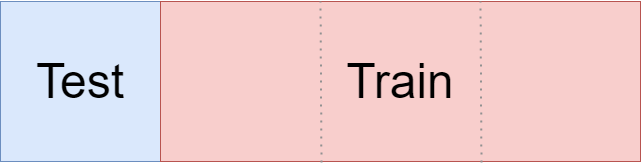
\includegraphics[width=70mm,scale=0.5]{images/regression_images/training_and_test_data_4.png}
            
        \end{figure}
        
        We now have \textbf{four different hypotheses} for the price of one!\\
        
        \begin{definition}
            \vocab{Cross-validation} is a way to \gren{evaluate} a learning algorithm using \purp{limited data}.

            \begin{itemize}
                \item We do this by \purp{breaking} our data it into \gren{chunks} to create \orgg{multiple hypotheses} from one dataset.
                
                \item For each \gren{chunk}, we train one dataset on all the data \orgg{not in that chunk}. We get our \purp{test error} using the chunk \textbf{we left out}.
            \end{itemize}
            
            For $k$ chunks, we end up with $k$ hypotheses. By \gren{averaging} out their performance, we can \purp{approximate} the quality of our algorithm.
        \end{definition}
        
        This approach is much \textbf{less expensive}, and very common in machine learning! 
            \note{But, some of the theoretical \textbf{benefits} of validation are not \textbf{proven} to be true for cross-validation.}\\
        
        \begin{clarification}
            Note that the goal of validation and cross-validation is \textbf{not} to evaluate \purp{one hypothesis}.
            
            Instead, it is instead meant to evaluate a \purp{learning algorithm}. This is why we have to create \purp{many} hypotheses: we want to see that our algorithm is \gren{generally} good!
        \end{clarification}
        
    \subsection{Hyperparameter Tuning}
    
        Now, we know how to \textbf{evaluate} a learning algorithm, just like how we \textbf{evaluate} a hypothesis. 
        
        Once we knew how to evaluate a hypothesis, we started optimizing our \gren{parameters} for the \textbf{best} hypothesis. So, we could do the same for our \textbf{learning algorithm}.

        How do we \orgg{optimize} a learning algorithm?
        
        Each $\lambda$ value creates a slightly \textbf{different} learning algorithm: we can \textbf{optimize} this \textbf{hyperparameter} to create the \textbf{best} learning algorithm.
        
    \subsection{How to tune our algorithm}
    
        When we were \textbf{optimizing} our hypothesis, we started by \textbf{randomly} trying hypotheses. Then, we used an \textbf{analytical} approach.
        \note{By "analytical", we mean directly creating an equation, and solving it.}
        
        We don't always have \textbf{simple} equations to work with: with all of our data, it's hard to come up with \textbf{manageable} equations. So, we \textbf{won't} try doing it \textbf{analytically}.
        
        So, we could \textbf{randomly} try $\lambda$ values and pick the \textbf{best} one. This is pretty \textbf{close} to what we usually end up doing. For each value we pick, we'll use \gren{cross-validation} to evaluate.
        
        For now, we'll systematically go through $\lambda$ values: $\lambda=.1, .2, .3 \dots$\\
        
        \begin{concept}
            \vocab{Hyperparameter tuning} is how we \purp{optimize} our \gren{learning algorithm} to create the \purp{best} hypotheses.
            
            The simplest way to do this is to try \gren{multiple} different values of $\lambda$. For each value, we use \gren{cross-validation} to evaluate that learning algorithm.
            
            Finally, we pick whichever $\lambda$ gives you the \purp{best} algorithm, and thus the \purp{best} hypotheses.
        \end{concept}
        
    \subsection{Hyperparameter Tuning: Two kinds of optimization}
    
        There's something often \textbf{confusing} about hyperparameter tuning to students:
            \note{In case the word "optimization" starts to look like gibberish in this section, remember: it just means, "find the best option".}

        \begin{itemize}
            \item When we're \textbf{optimizing} $\lambda$, we try many values $\lambda_j$. Each $\lambda_j$ create a \purp{learning algorithm} we have to evaluate. 
            
            \item But a single learning algorithm is already an optimization problem: the learning algorithm is supposed to find $\Theta$.

                \begin{itemize}
                    \item So, we have to \orgg{optimize} $\Theta$, while we're in the middle optimizing $\lambda$.
                \end{itemize}
        \end{itemize}
        
        
        That means, \textbf{every time} we try a different $\lambda$ value, we have to do one optimization problem. Optimizing $\Theta$ many times, lets you optimize $\lambda$ once.
            \note{Remember that, in this situation, $\Theta$ and $h$ are almost(but not quite) the same thing.}

        \begin{equation*}
                \begin{rcases}
                \begin{matrix}
                    \data_n \longrightarrow 
                    \boxed{\text{learn alg using $\red{\lambda_1}$}} 
                    \longrightarrow \Theta_1
                    \longrightarrow
                    \boxed{\text{Test error }}
                    \longrightarrow 
                    \overbrace{\testerr(h_1)} ^{\text{Evaluates }\red{\lambda_1}} \\\\
                    \data_n \longrightarrow 
                    \boxed{\text{learn alg using $\red{\lambda_2}$}} 
                    \longrightarrow \Theta_2
                    \longrightarrow
                    \boxed{\text{Test error }}
                    \longrightarrow 
                    \overbrace{\testerr(h_2)} ^{\text{Evaluates }\red{\lambda_2}} \\
                    \vdots \\
                    \data_n \longrightarrow 
                    \boxed{\text{learn alg using $\red{\lambda_n}$}} 
                    \longrightarrow \Theta_n
                    \longrightarrow
                    \boxed{\text{Test error }}
                    \longrightarrow 
                    \overbrace{\testerr(h_n)} ^{\text{Evaluates }\red{\lambda_n}}
                \end{matrix}
                \end{rcases}\text{Pick best $\lambda_j$ using $\testerr$}  
            \end{equation*}
        
        That means we have \textbf{two layers} of optimization!\\
        
        \begin{clarification}
            We \purp{optimize} $\lambda$ by trying many values.

            \begin{itemize}
                \item But, for each $\lambda$ value, we have to \gren{optimize} $\Theta$.
            \end{itemize}
            
            So, we have to optimize $\Theta$ \purp{repeatedly} in order to optimize $\lambda$ \purp{once}! This gives us $\lambda^*.$
        \end{clarification}
        
        Once we've found our best hyperparameter $\lambda^*$, we can use it to get our best parameters: $\theta^*$.
        
    \subsection{Pseudocode Example}
        
        This technique is \textbf{not} limited to regression. Thus, we'll be a bit more \textbf{general}: we won't assume an \textbf{analytical} solution. Instead, we \textbf{optimize} by just trying different $\Theta$ values.
        
        We can represent this in pseudocode:
        \note{If this pseudocode isn't helpful to you, don't worry! Some students like it, some don't.}
        
        \begin{codebox}
            \Procname{$\proc{Lambda-Optimization}
                       (\data, lambda\_values, theta\_values)$}
                       
                \li \For $\lambda$ \In $lambda\_values$        
                \qquad\quad\#Try lambda values
                
                \li     \Do \For $\Theta$ \In $theta\_values$  
                \qquad\quad\#Try theta values    
                            \Do

                                \li Calculate $J(\Theta)$    
                                \qquad\qquad\qquad\#Compare values
                            \End
                        
                        \li Choose best theta value $\Theta^*$ 
                        \quad\#Best for each lambda

                        \End
                \li Choose best lambda value $\lambda^*$
                \li
                    
                \li \Return $\lambda^*$
        \end{codebox}
        
    To reiterate: this $\lambda^*$ will then we used to get our final result, $\theta^*$.

\pagebreak
        
\section{Terms}

    \begin{itemize}
        \item Hypothesis
        \item Theta ($\Theta$)
        \item Input Space
        \item Regression
        \item Feature
        \item Feature Transformation
        \item Training Error
        \item Test Error
        \item Objective Function
        \item Min function
        \item Argmin function
        \item Star Notation ($\theta^*$)
        \item Linear Regression
        \item Hypothesis Class
        \item Square Loss
        \item Ordinary Least Squares (OLS) Problem
        \item OLS Objective Function
        \item Hyperplane
        \item Weight
        \item Input Matrix
        \item Output Matrix
        \item Gradient
        \item OLS Solution
        \item Regularization
        \item Regularizer
        \item Regularizer for Regression
        \item Lambda ($\lambda$)
        \item Ridge Regression
        \item RR Objective Function
        \item RR Solution
        \item Invertibility
        \item Estimation Error
        \item Structural Error
        \item Expressiveness
        \item Learning Algorithm
        \item Hyperparameter
        \item Validation
        \item Cross-Validation
        \item Chunk (Cross-Validation)
        \item Hyperparameter Tuning
    \end{itemize}
        
        
        






%%% Local Variables:
%%% mode: latex
%%% TeX-master: "top"
%%% End:

% \setcounter{chapter}{2}

\chapter{Gradient Descent}

\label{chap:gradient}

\section*{What is gradient descent?}


    \subsection{Why do we need gradient descent?}

        In the last chapter, we used an \textbf{analytical} approach to solve the OLS and RR problems.
        
        By "analytical", we mean we got an \textbf{explicit} answer: an equation we can use to directly compute the correct answer.
        
        The trouble is, we can't always do this:
        
        \begin{itemize}
            \item Sometimes the problem or the loss function can't be \textbf{rearranged} into a simple \textbf{equation}. 
            
            \item Or, we have \textbf{too much} data, and directly computing the answer would take way \textbf{too long}.\\
        \end{itemize}
        
        \begin{concept}
            Most \vocab{problems} we come across cannot be solved \vocab{analytically}.
        \end{concept}
        
        Well, if we can't \textbf{directly} find the \textbf{best} answer, what's the next best thing? Finding a \textbf{better} solution than your current one.
        
        So, our mission is to gradually try to find a better and better answer. This type of approach has a couple benefits:
        
        \begin{itemize}
            \item It's \textbf{quicker} to see if we're using a good model: if we're making very little progress, we can \textbf{quit} early and try something else.
            
            \item If we don't need \textbf{all} of our data to get the answer, we don't need to spend as much time. If our answer is \textbf{good} and not getting better, we can \textbf{stop}.
            
            \item It's easier to find a \textbf{better} answer than the \textbf{best} answer: our equations will be \textbf{simpler}. In some case, it might not have even been \textbf{possible} without this gradual approach!\\
        \end{itemize}
        
        \begin{concept}
            When we can't reasonably find a \purp{best} answer, it's often easier to find a \gren{better} answer and gradually \gren{improve}.
            
            \vocab{Gradient descent} follows this philosophy: we gradually \purp{update} our solution to make it better and better.
        \end{concept}
        
        
        
    \subsection{How do we improve?}
    
        So, now, the question is: how do we \textbf{improve} our hypothesis? We'll be modifying our hypothesis $\theta$ by some amount:
            \note{We'll do the same for $\theta_0$, but we'll do it separately. We'll come back to that.}
        
        \begin{equation}
            \theta_{new} = \theta_{old} + \Delta \theta
        \end{equation}
        
        \begin{notation}
            In equations, we'll often use $\theta_{old}$ and $\theta_{new}$ to represent \gren{before} and \purp{after} we take a step.
            
            We will use this notation \textbf{elsewhere} in the class.
        \end{notation}
        
        So, we are interesting in $\Delta \theta$: how do we plan to change $\theta$? What does $\Delta \theta$ look like?
        
        Well, we want to modify
        
        \begin{equation}
            \theta = 
            \begin{bmatrix}
                \theta_1 \\ \theta_2 \\ \vdots \\ \theta_d
            \end{bmatrix}
        \end{equation}
        
        So, we want to modify each of those terms.
        
        \begin{equation}
            \theta 
            = 
            \begin{bmatrix}
                \theta_1 \\ \theta_2 \\ \vdots \\ \theta_d
            \end{bmatrix}
            +
            \begin{bmatrix}
                \Delta \theta_1 \\ \Delta \theta_2 \\ \vdots \\ \Delta \theta_d
            \end{bmatrix}
        \end{equation}
        
        So, we have our total change!
        
        \begin{equation}
            \Delta \theta 
            = 
            \begin{bmatrix}
                \Delta \theta_1 \\ \Delta \theta_2 \\ \vdots \\ \Delta \theta_d
            \end{bmatrix}
        \end{equation}
        
        Notice that the shape of this change matches the shape of $\theta$: $(d \times 1)$.\\
        
        \begin{concept}
            We need a \purp{separate} term $\Delta \theta_i$ for each $\theta_i$ we want to \gren{improve}.
            
            So, a vector of the \purp{total} change, $\Delta \theta$, needs to have the \gren{same shape} as $\theta$: $(d \times 1)$.
        \end{concept}
        
        
    \subsection{The name: "gradient descent"}
    
        Our goal is to gradually \textbf{decrease} $J$, step-by-step. We do this using the \textbf{gradient}, hence "gradient descent". Why the gradient? We'll discuss that later.
        
        But why the word "\textbf{descent}"? 
        
        Our intuition is to imagine $J$ as having a \textbf{height} at every input value. If you combine all of these different points, you get a \textbf{surface}, like the surface of a hill.
        
        \begin{figure}[H]
            \centering
                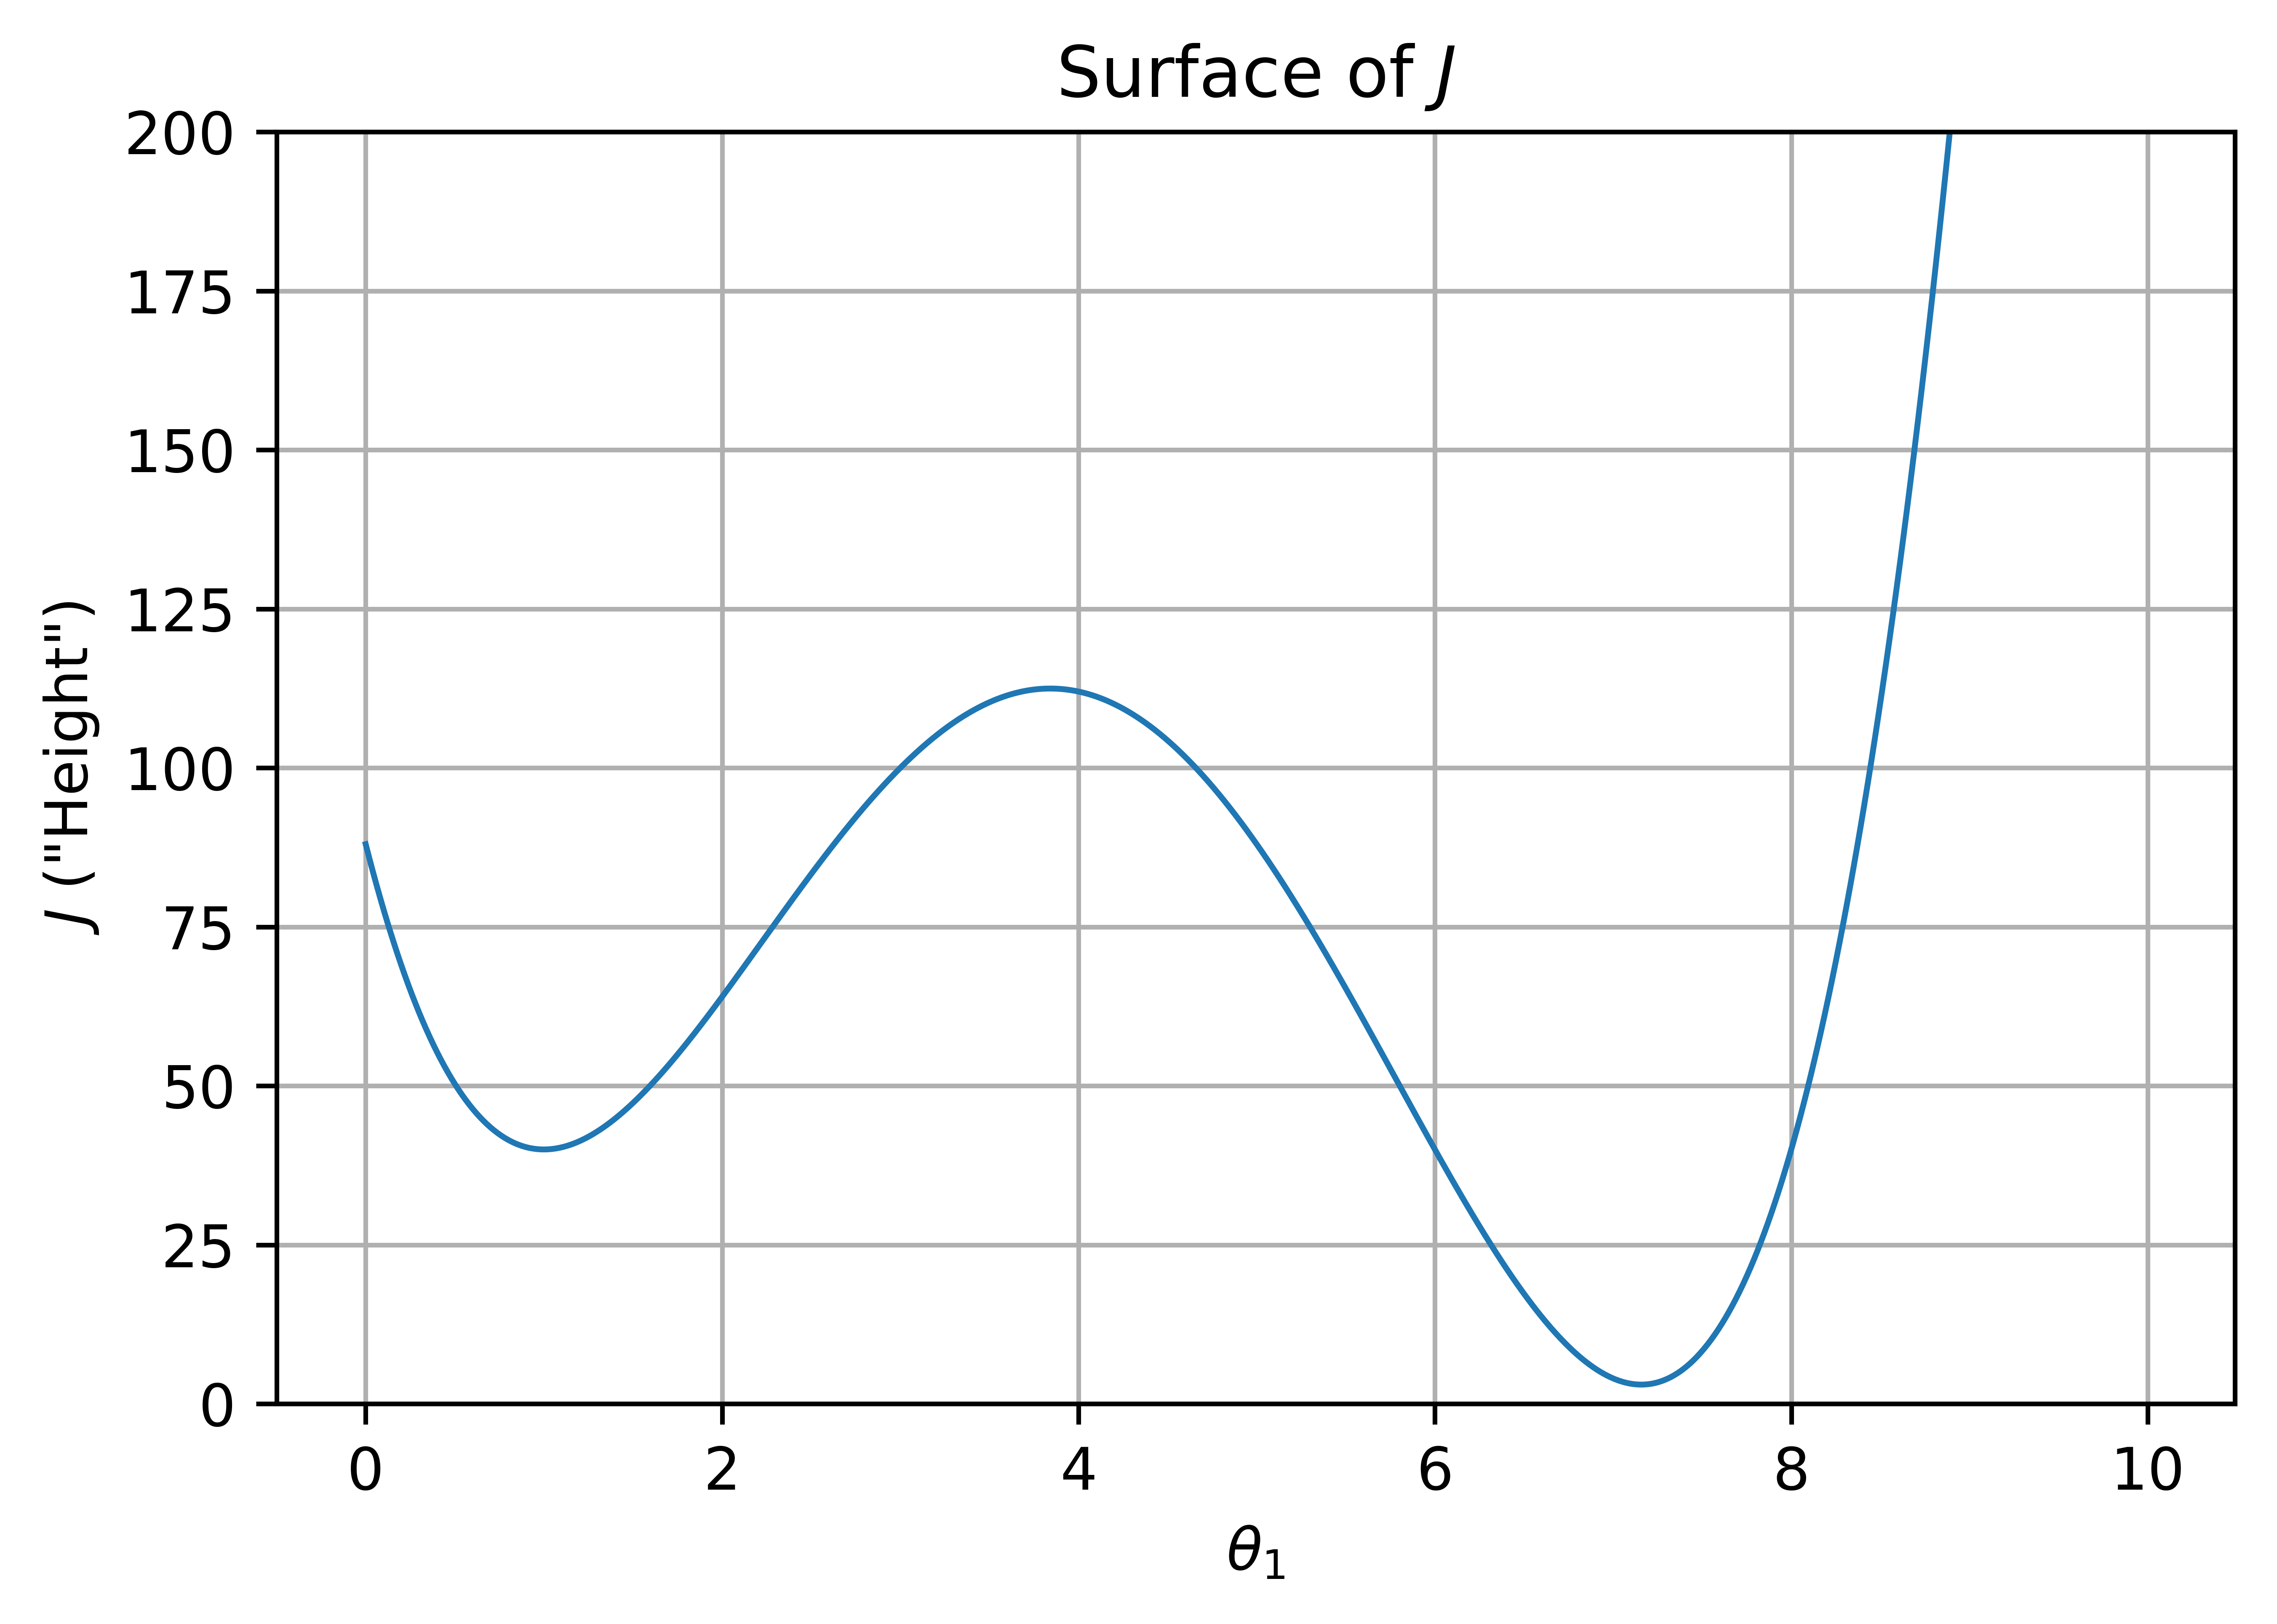
\includegraphics[width=70mm,scale=0.5]{images/gradient_descent_images/Surface_of_J.png}
            
            \caption*{You can imagine this like some hills we want to "descend".}
        \end{figure}
        
        Then, decreasing $J$ is moving \textbf{down} the the function, similar to rolling a ball down a hill. In other words, we \textbf{descend} the hill.
        
        \begin{figure}[H]
            \centering
                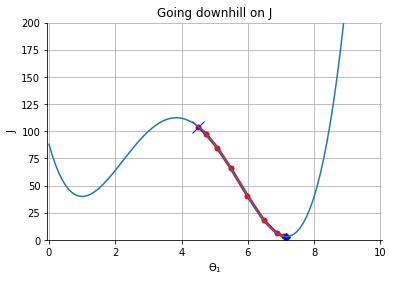
\includegraphics[width=70mm,scale=0.5]{images/gradient_descent_images/going_downhill.png}
            
            \caption*{Like this! Starting from the blue "X", moving 'downhill'.}
        \end{figure}
        
    \subsection{Input Space vs. Parameter Space}
    
        One more thing to note: we have two similar situations.
        
        \begin{itemize}
            \item $J$ is a \textbf{function} with $\theta$ as an \textbf{input}: $J(\theta)$.
            
            \item $h$ is a \textbf{function} with $x$ as an \textbf{input}: $h(x)$. 
        \end{itemize}
        
        In both cases, we can imagine the \textbf{output} as the "\textbf{height}" of our function: the \textbf{hill} we mentioned before. This \textbf{physical} intuition is useful to \textbf{gradient descent}.
        
        But, what about \textbf{input} to our function? That's the x-axis our hill is floating above:
        
        \begin{itemize}
            \item With $h(x)$, our x-axis was our \textbf{input space}, all possible $x_1$ values: the "space" containing all of our possible inputs.
            
            \item With $J(\theta)$, our x-axis is the \textbf{parameter space}, all possible $\theta$ values. We also called this our "\textbf{hypothesis space}".
                \note{We're assuming 1-D right now for simplicity. If we were 2-D, we'd have an entire 2D grid under our hill!}\\
        \end{itemize}
        
        \begin{definition}
            The \vocab{parameter space} is our set of all \gren{possible} parameter combinations.
            
            This is the same as the \vocab{hypothesis space}, because our parameters \gren{define} our hypothesis.
            
            When we \gren{optimize} our hypothesis, we are "\purp{exploring}" the hypothesis space. 
        \end{definition}
        
        This also gives us an idea of which hypotheses are "\textbf{similar}": those which are \textbf{closer} in parameter space (which we used, when we were doing regularization $\norm{\theta-\theta_{old}}$).
        
        This is the \textbf{space} we're exploring, as we try to move \textbf{downhill}. \\
        
        \begin{clarification}
            Pay attention to your \purp{axes}! 
            
            Sometimes, we're doing a 2-D or 3-D plot of $J$, and our inputs are $\theta_k$. Other times, we're plotting hypothesis $h$, with our axes $x_i$.
            
            These two plots could have the same surface, but they \gren{represent} completely different things.
        \end{clarification}
        

        
        

        
\pagebreak

%%%%%%%%%%%%%%%%%%%%%%%%%%%%%%%%%%%%%%%%%%%%%%%%%%%%%%%%%%%%%%%%%%%%%%%%%%%%%%%%%%%%%%%%%%%
\section{Gradient Descent in One Dimension}

    \subsection{Derivatives (Review)}
    
        Here, we'll use some concepts from \textbf{calculus}.
        
        We'll make improvements in small \textbf{steps}. And, we measure our improvement against the \textbf{loss function}, $J$: that's what we want to \textbf{optimize}.
        
        In calculus, we found that, over \textbf{small} enough steps, you can \textbf{approximate} as function as a straight line.\\
        
        \begin{figure}[H]
            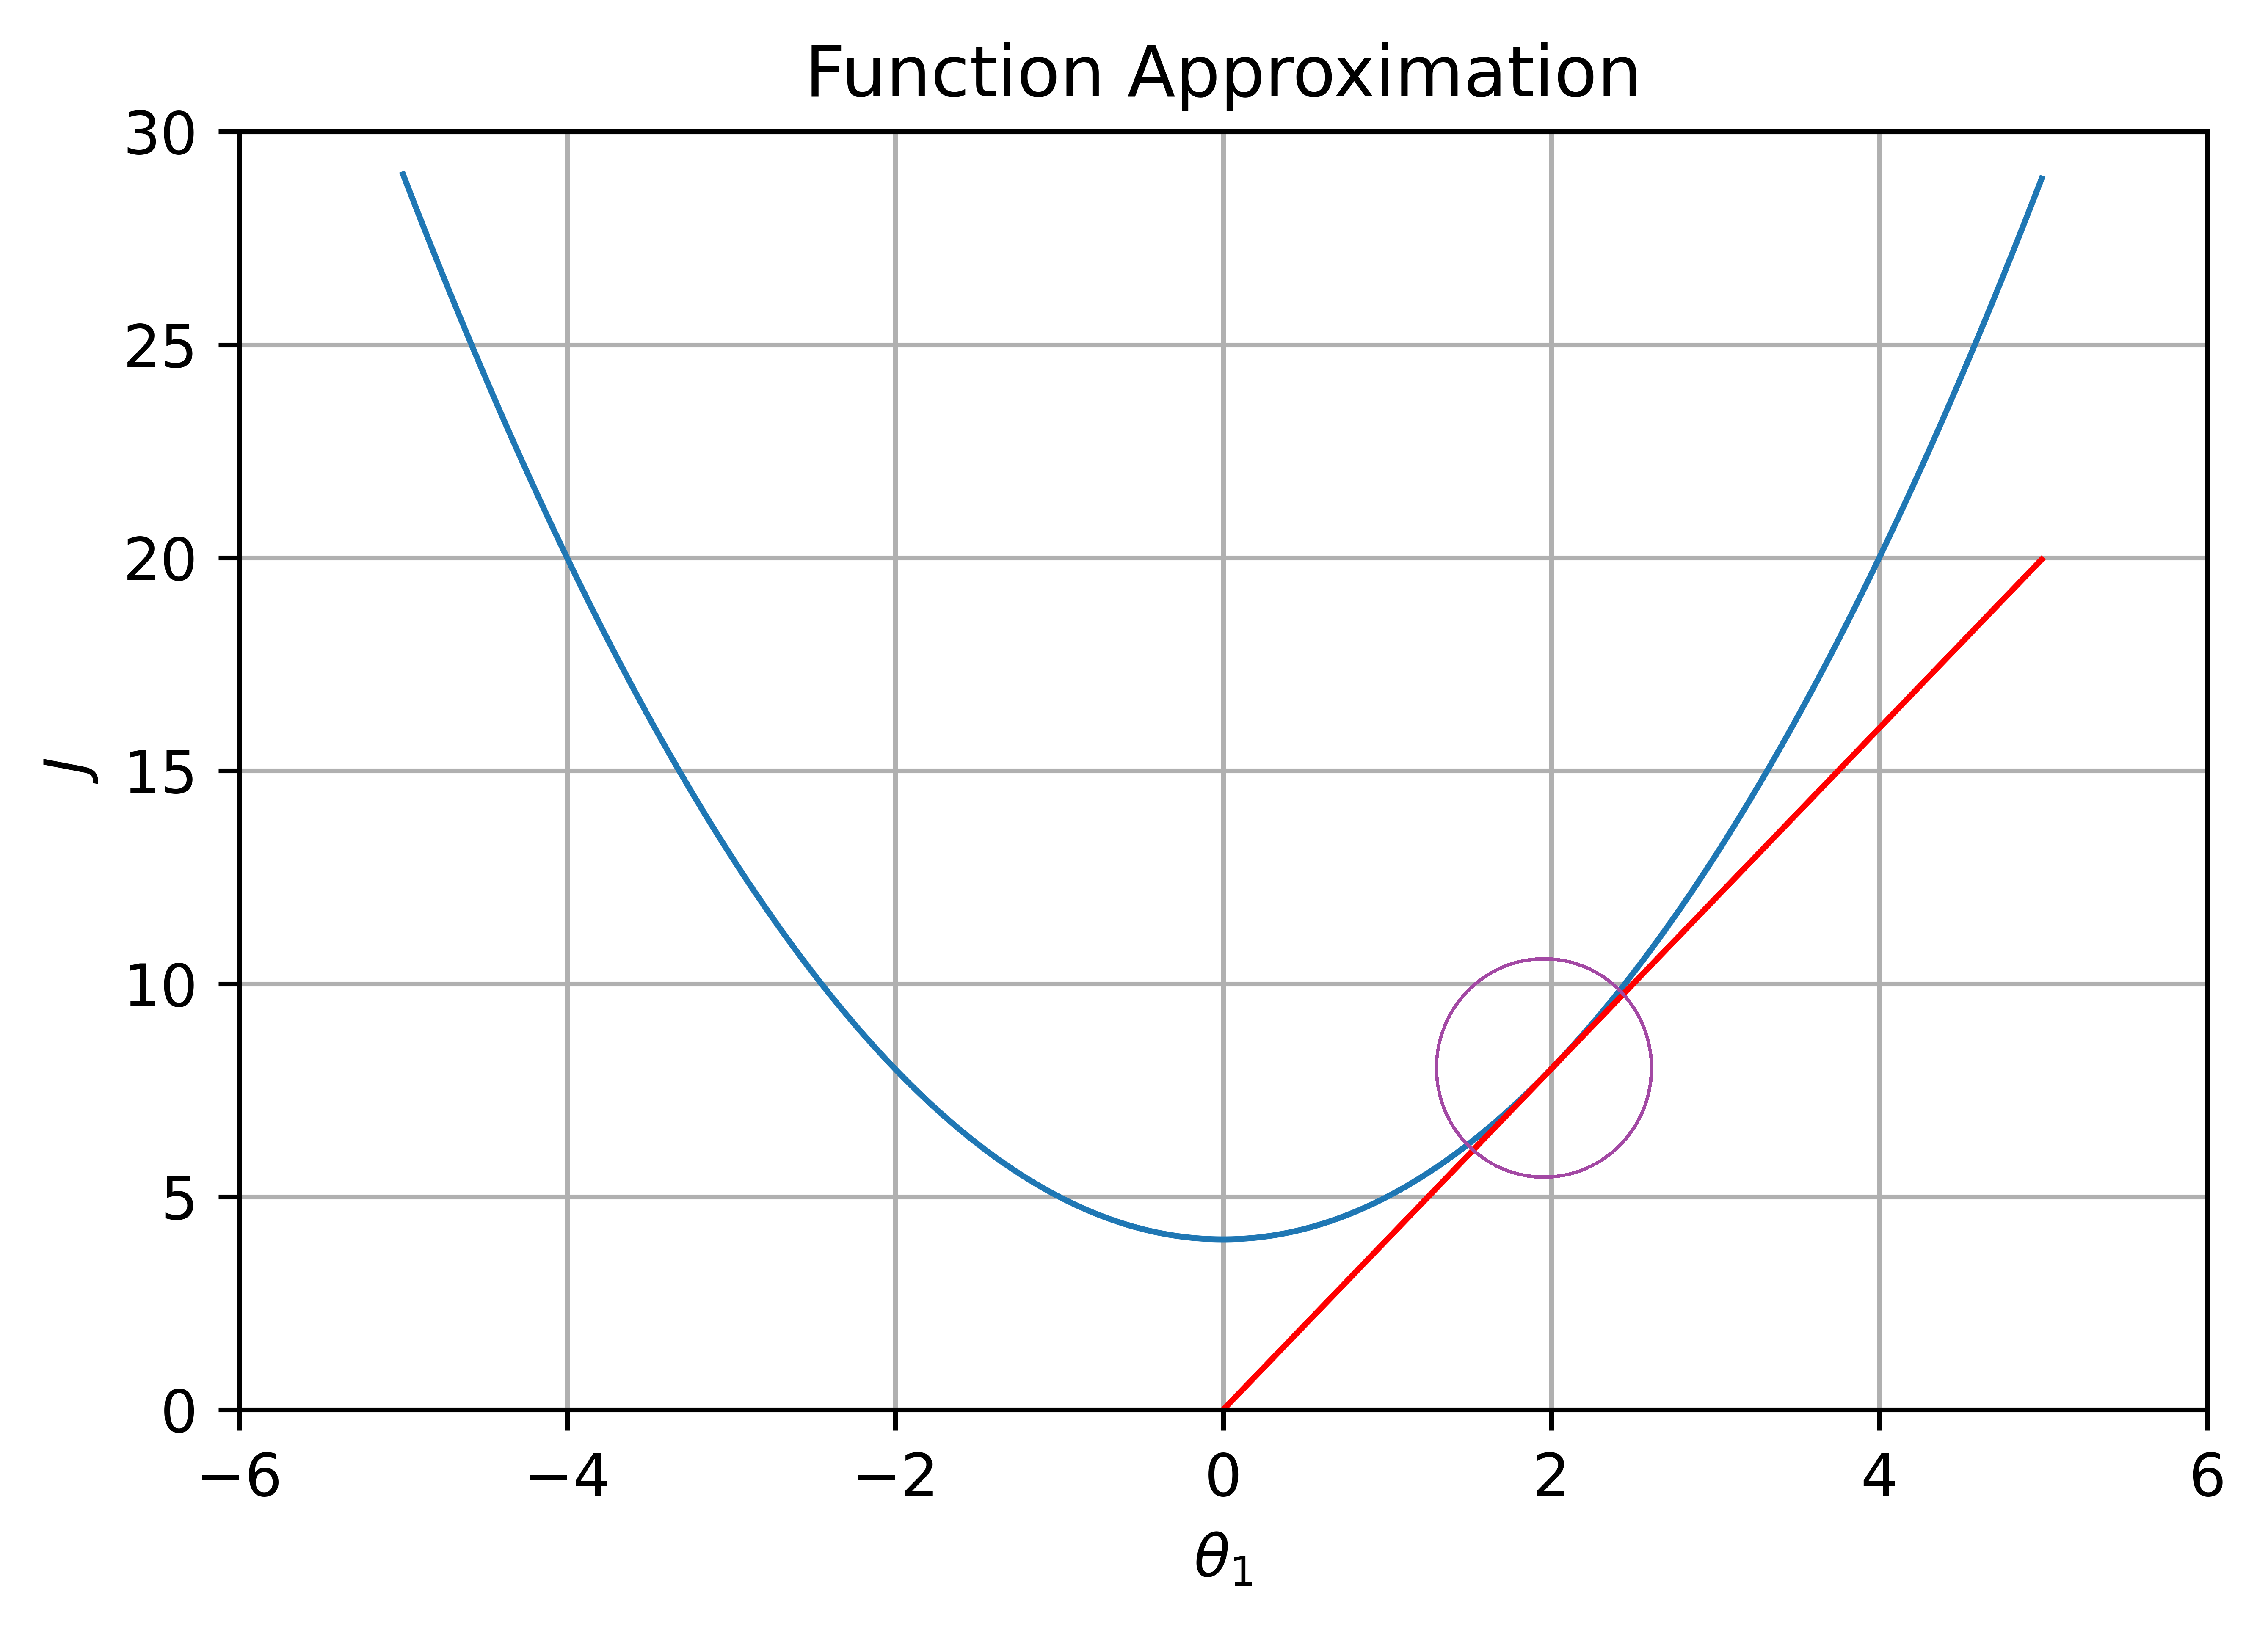
\includegraphics[width=70mm,scale=0.5]{images/gradient_descent_images/function_approximation_linear.png}
            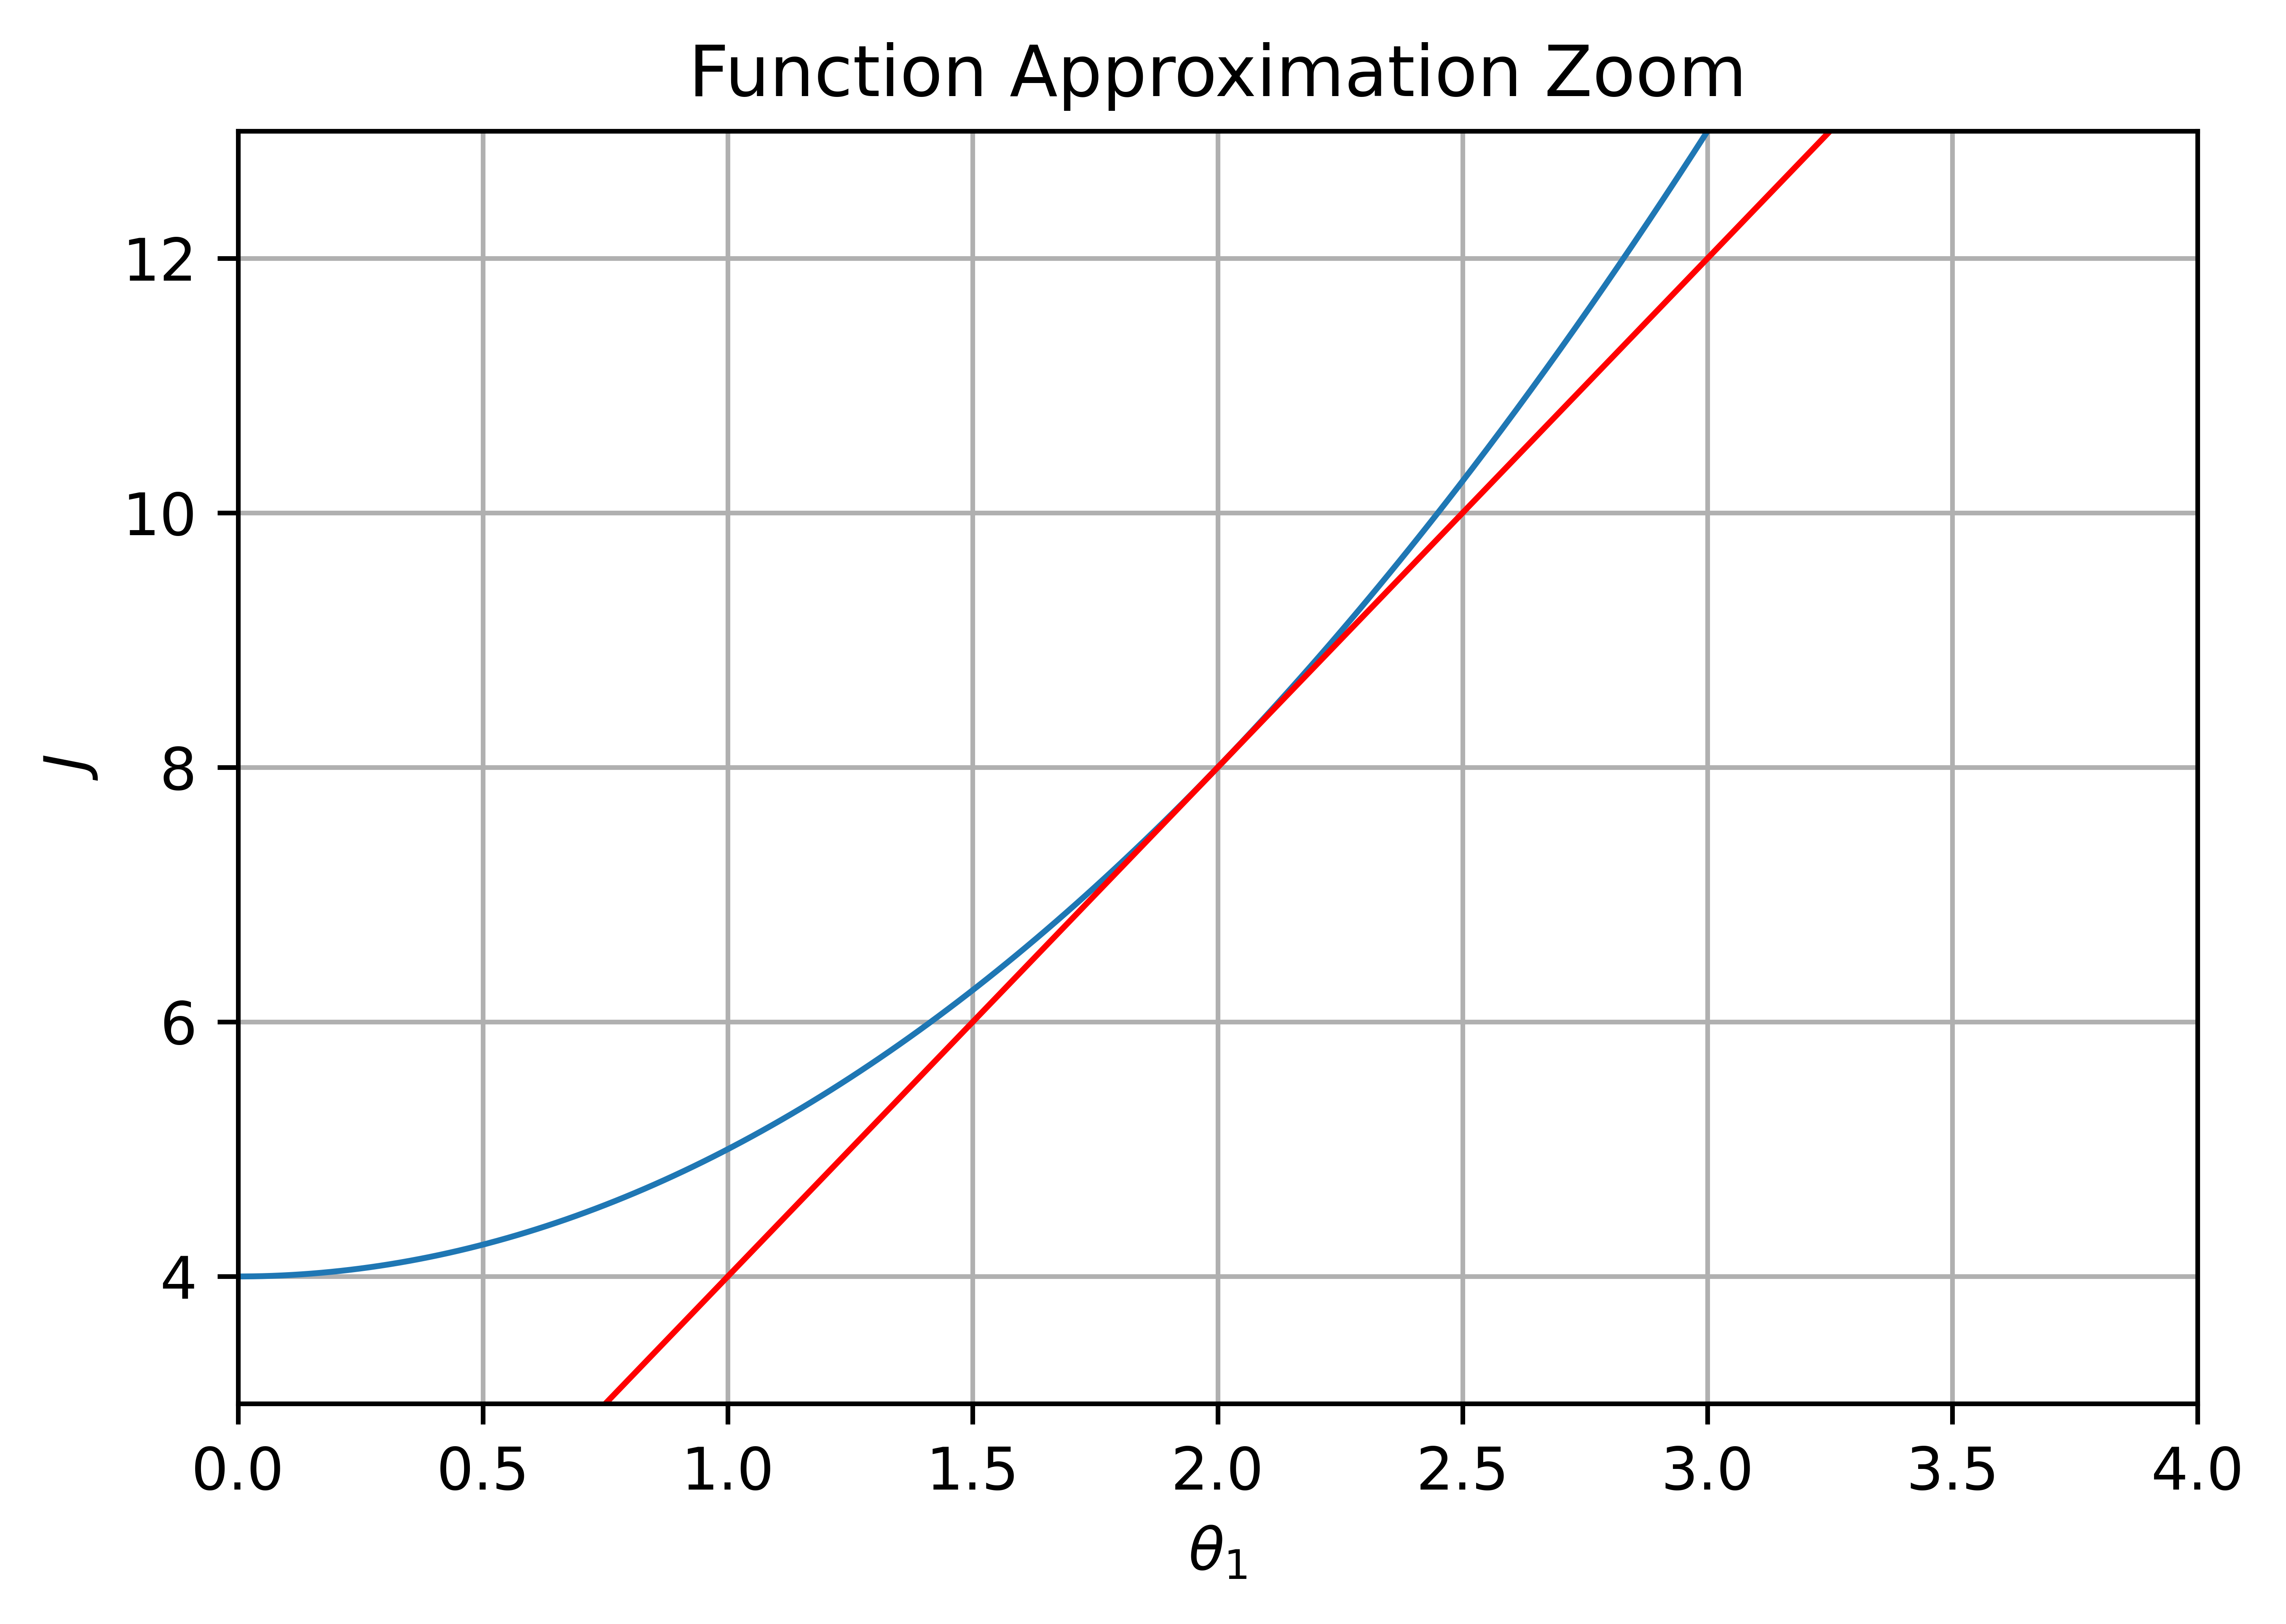
\includegraphics[width=70mm,scale=0.5]{images/gradient_descent_images/function_approximation_linear_zoom.png}
            
            \caption*{It looks more like a line as we zoom in: hence the \textbf{local} approximation.}
        \end{figure}
        
        %%Insert figure
        
        \begin{concept}
            A \gren{smooth} (enough) function can be \purp{approximated} with a \vocab{straight line} if you \purp{zoom} in on it enough.
            
            Looking at it this way is called a \vocab{local} view.
        \end{concept}
        
        
        
    \subsection{Optimize with Derivatives: 1-D}
        
        This gives us the \textbf{slope} of the function locally. Last chapter, we used $\deriv{J}{\theta}=0$ to get our \textbf{minimum}.
        
        But, let's not get too greedy - we want to \textbf{improve} our hypothesis, \textbf{not} immediately try to find the \textbf{best} one.
            \note{Because the best one might be expensive to find this way!}
        
        Well, what does our slope tell us? It tells us:
        
        \begin{itemize}
            \item How quickly $J$ changes
            \item Whether it \textbf{increases} or decreases as we change $\theta$
        \end{itemize}
        
        That second one tells us \textit{how to change} $\theta$: we want to move in the direction that \textbf{decreases} $J$.
        
        If the slope is \textbf{positive}, then we want to \textbf{decrease} $\Delta \theta$: the sign of $\Delta \theta$ is the opposite of our desired change!
        
        \begin{figure}[H]
            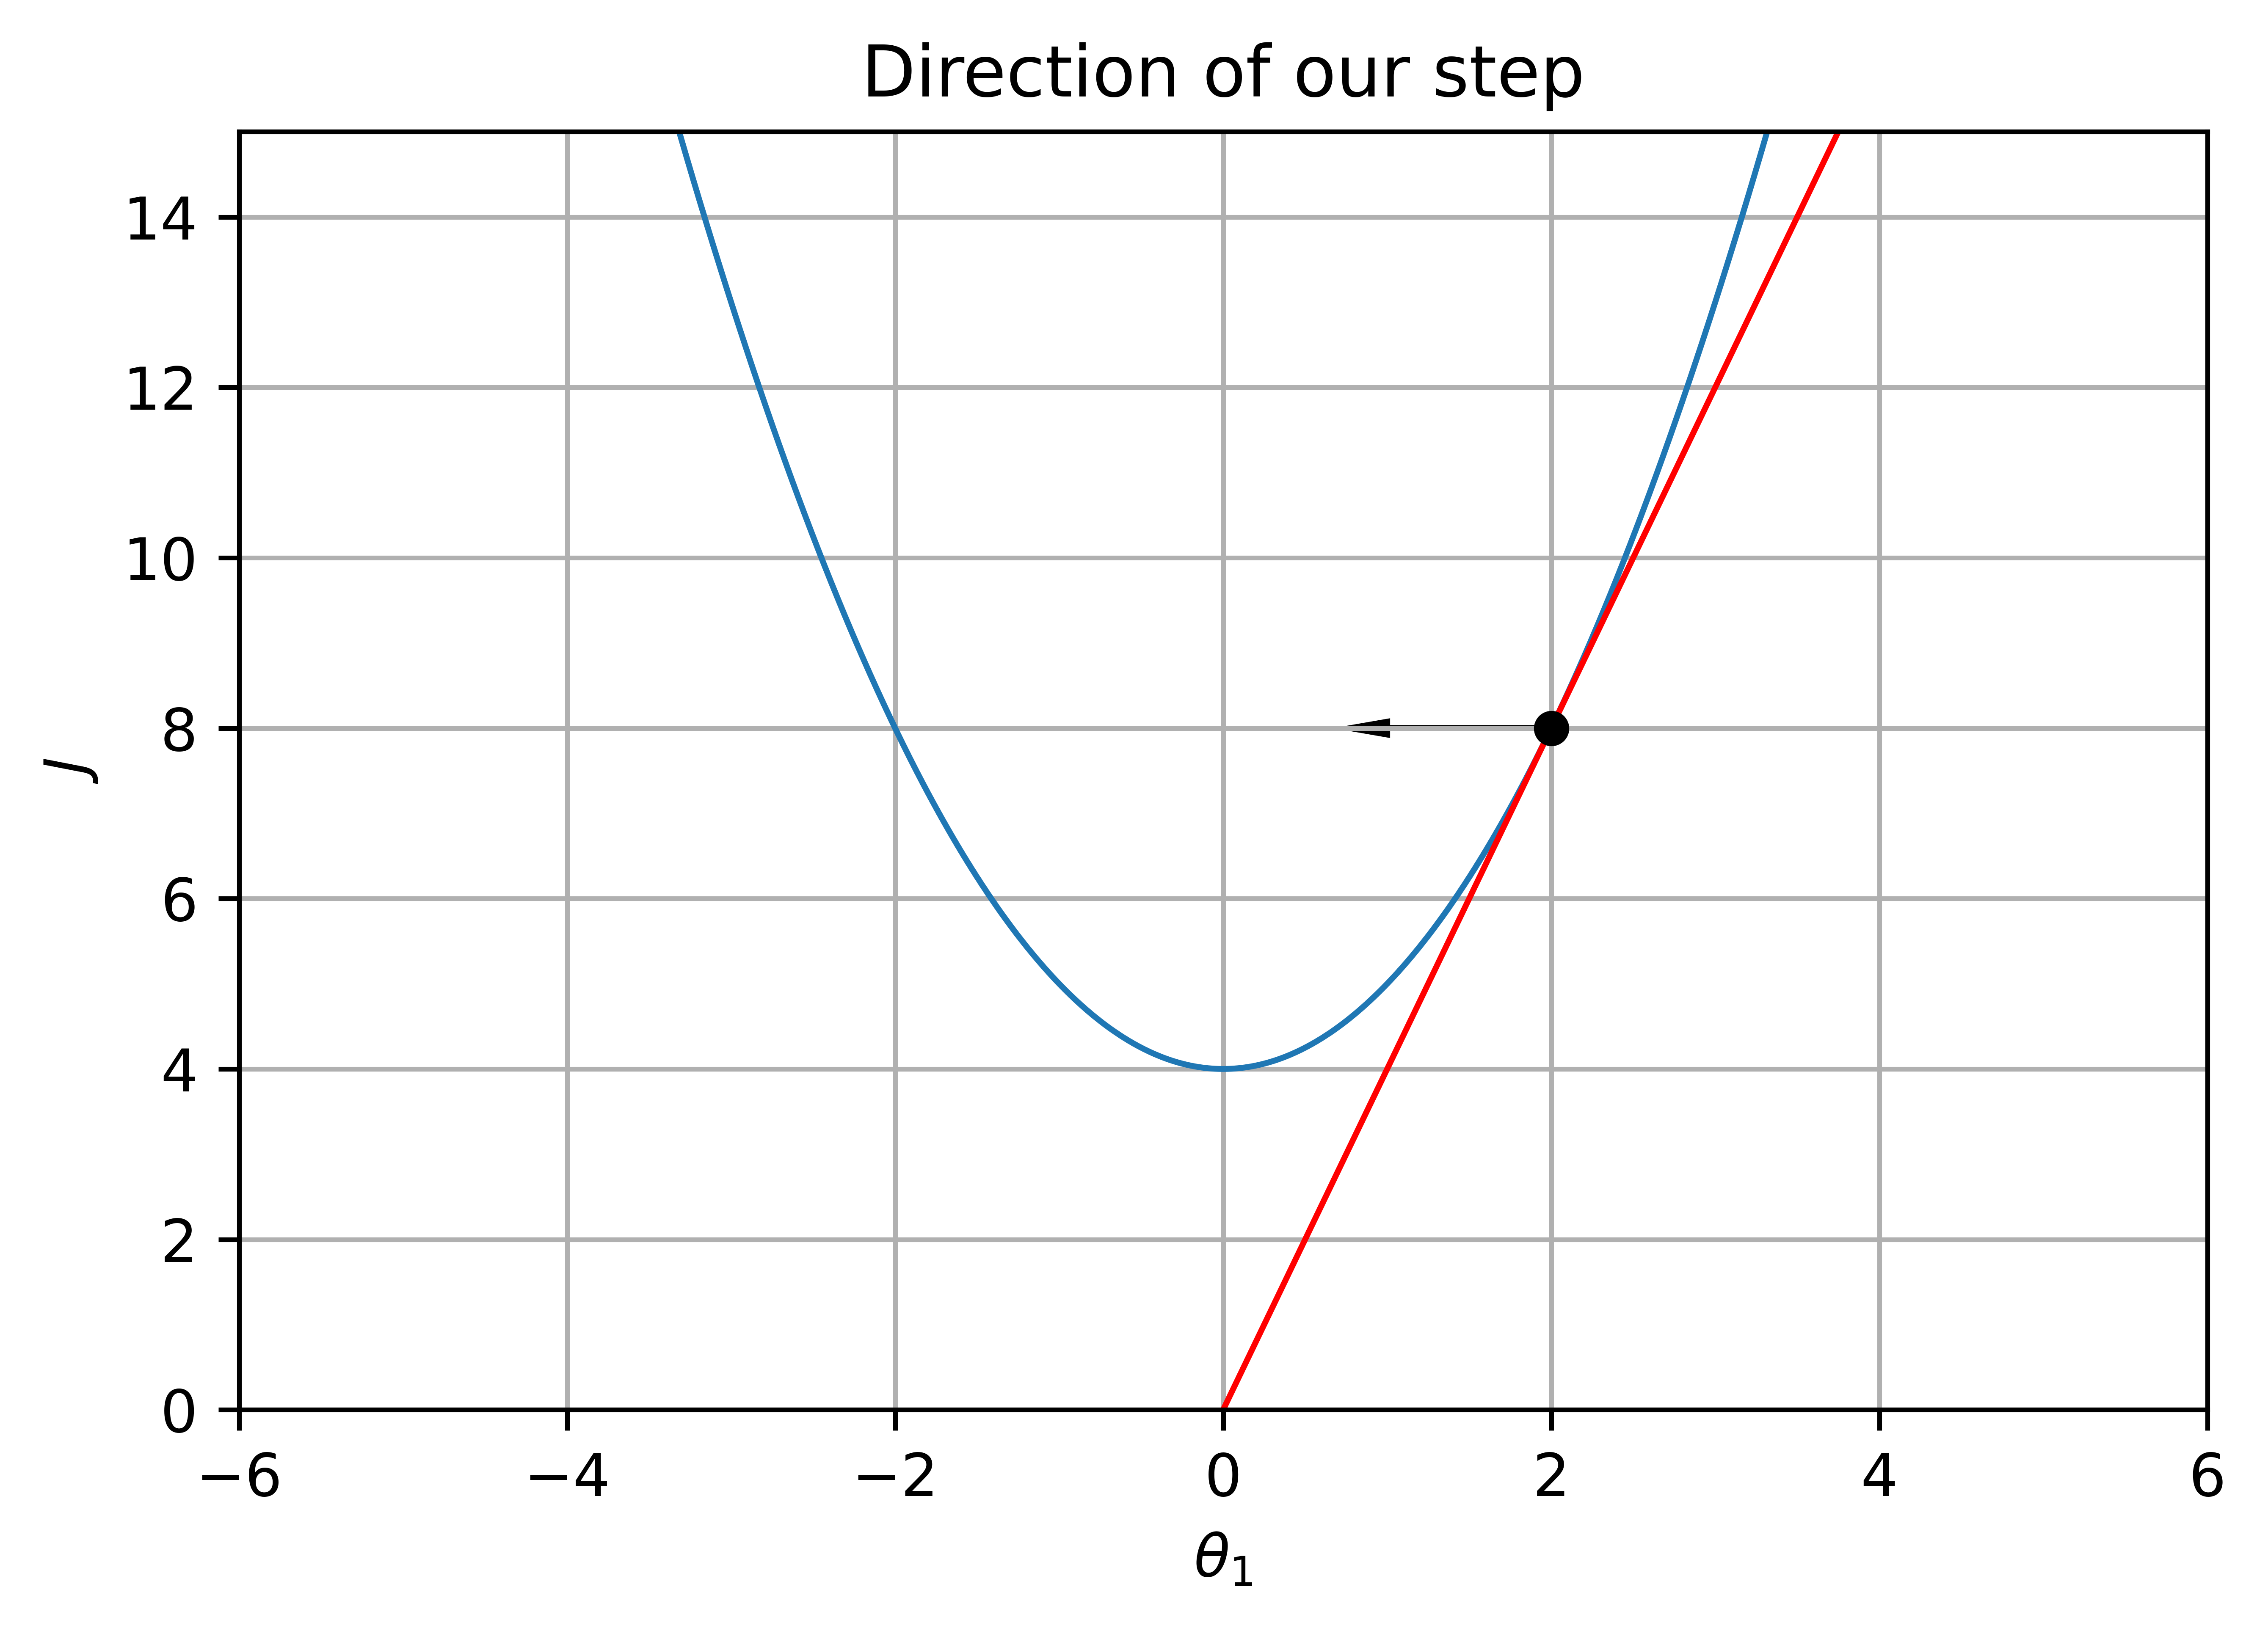
\includegraphics[width=70mm,scale=0.5]{images/gradient_descent_images/taking_a_step.png}
            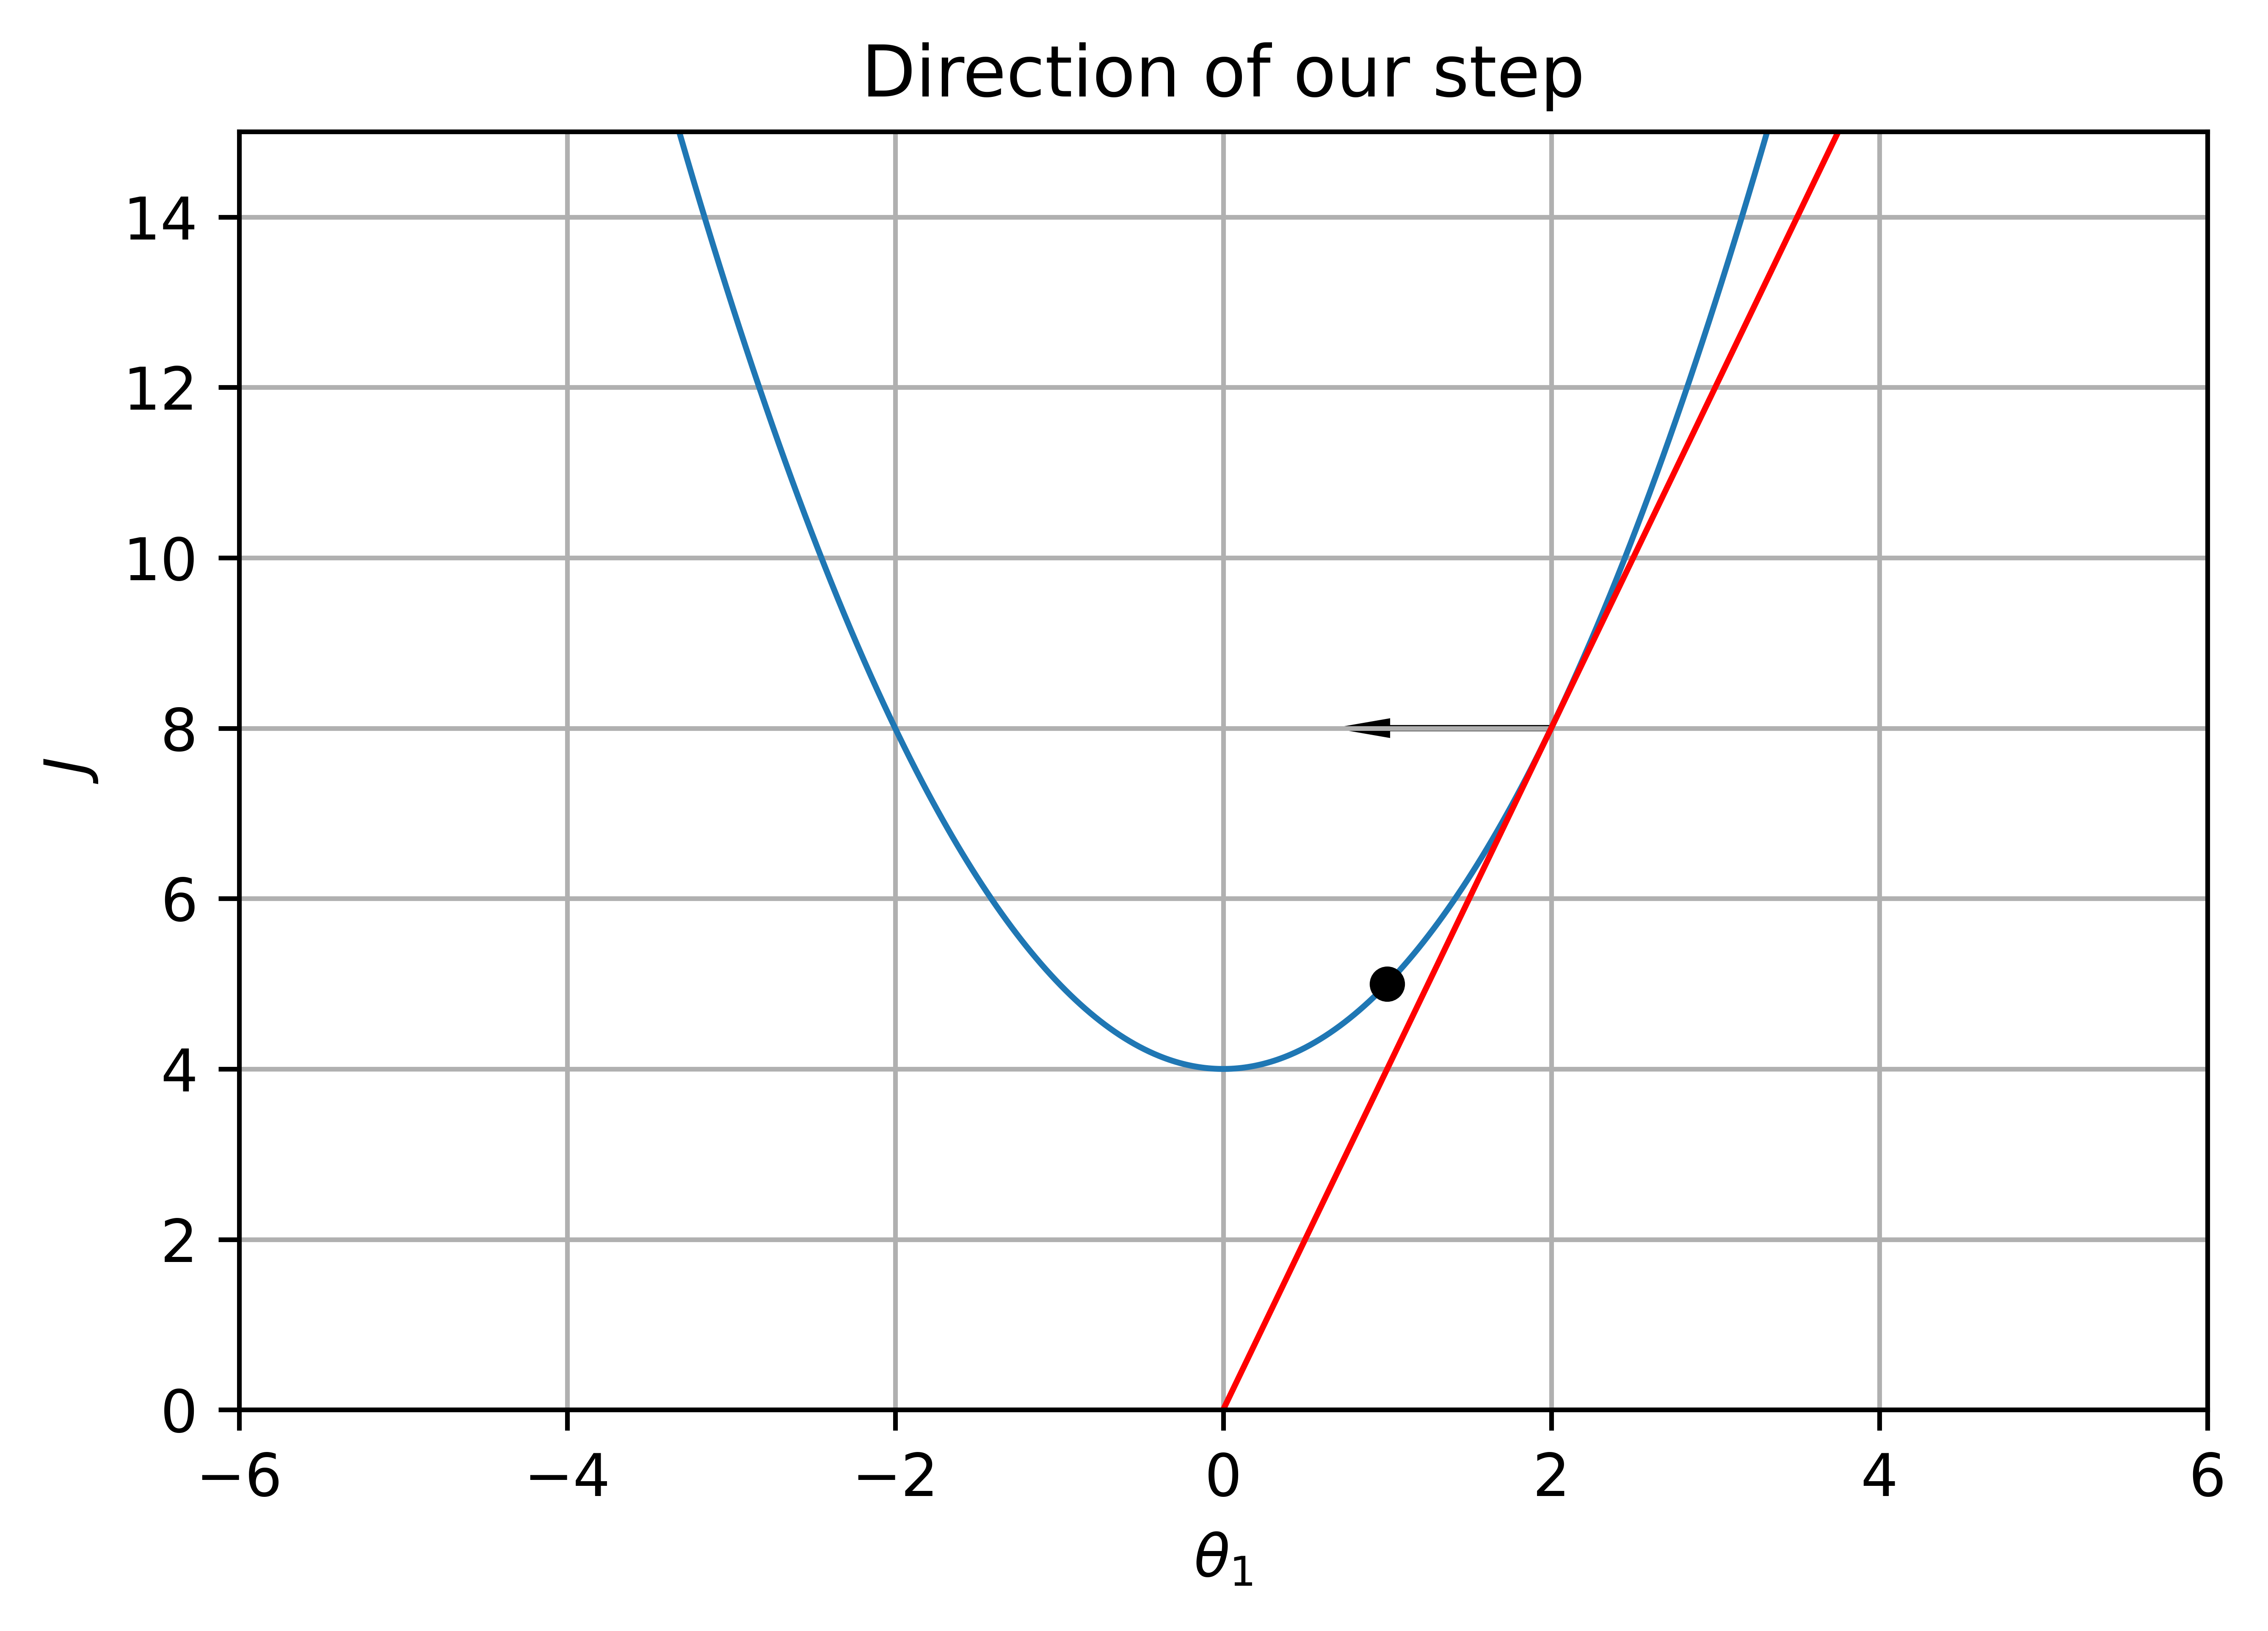
\includegraphics[width=70mm,scale=0.5]{images/gradient_descent_images/took_a_step.png}
            
            \caption*{Our slope is \textbf{positive}. We want to \textbf{decrease} our function, so we move in the \textbf{negative} direction, and "fall down" the surface.}
        \end{figure}
        
        And so, for now, we have
        
        \begin{equation}
            \Delta \theta = -\deriv{J}{\theta}
        \end{equation}\\
        
        \begin{concept}
            In \vocab{1-D}, you can use the \vocab{derivative} to \gren{optimize} our function $J$.
            
            The \purp{derivative} tells us how to immediately adjust $\theta_i$ to \gren{improve} our $J$ \purp{locally}: we move in the \gren{opposite direction}.
        \end{concept}
        
        This gives us a procedure for optimizing $J$: get the derivative $J'(\theta)$, and repeatedly adjust $\theta$ in the opposite direction until you're satisfied.
            \note{We'll need to pick a condition for being satisfied, but we'll get to this later}
        
        There's a certain way this feels like we're moving "\textbf{downhill}": we're moving "down" the slope, to try to find a local \textbf{minimum}.
        
    \subsection{Convergence}
    
        If you do this procedure with the above equation, though, you'll often run into \textbf{problems}. Why is that?
        
        Well, because each of your steps is too \textbf{big} or too \textbf{small}: we won't be able to find a \textbf{stable} answer, i.e. \textbf{converge}!
        
        What does it mean to \textbf{converge}? 
        
        It means we get a \textbf{single answer} after repeated steps: given enough time, we'll get \textbf{close as we want} to one number, and \textbf{stay there}.\\
        
        \begin{definition}
            If a sequence \vocab{converges}, then our result gets as \purp{close as we want} to a \gren{single number}, without going \purp{further away}.
        \end{definition}
        
        \miniex The numbers $1/n$: $\{ 1, \frac{1}{2}, \frac{1}{3}, \frac{1}{4}, \dots  \}$ converges to 0.
        
        If our answer \textbf{doesn't} converge, then it \textbf{diverges}. We can see why this might be bad: if we never \textbf{approach} a single answer, how do we know what value to \textbf{pick}?
        
    \subsection{Convergence: A little more formally (Optional)}
        
        Let's be more specific. Our sequence $S$ will converge to $r$.
        
        \begin{equation}
            S = \{ s_1, s_2, s_3, s_4, \dots \} 
        \end{equation}
        
        "As close as we want": let's say we want the maximum distance to be $\epsilon$. That means, no matter what $\epsilon>0$, we'll get closer at some point: $\abs{m-s_i}<\epsilon$
        
        \begin{equation}
            \abs{m-s_i}<\epsilon \text{ for some } i
        \end{equation}
        
        "And stay there": at some time $k$, we never move further away again:\\
        
        \begin{definition}
            If a sequence $S$ \vocab{converges} to $m$, then for all $\epsilon>0$, we can say
            
            \begin{equation}
                \abs{m-s_i}<\epsilon \text{ for all } i>k
            \end{equation}
        
        \end{definition}
        
        This is a "formal" definition of convergence.
        
    
    \subsection{Step size}
    
        If your steps are too \textbf{big}, your result might \textbf{diverge}: you make such big jumps, you move \textbf{away} from the minimum, and get worse.
            \note{Remember, if it \textbf{diverges}, it never \textbf{approaches} a single value!}
        
        \begin{figure}[H]
        \centering
            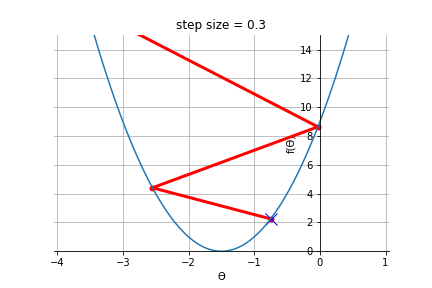
\includegraphics[width=70mm,scale=0.5]{images/gradient_descent_images/diverge.png}
        
        \caption*{We start at the blue "x" mark. Notice that, even though we try to move toward the minimum, we go too far and accidentally get further and further!}
        \end{figure}
        
        If they're too \textbf{small}, you might \textbf{converge} too slowly: it'll take way \textbf{too long} to make progress.
            \note{\textbf{Converging} means it successfully \textbf{approaches} an answer!}
        
        \begin{figure}[H]
        \centering
            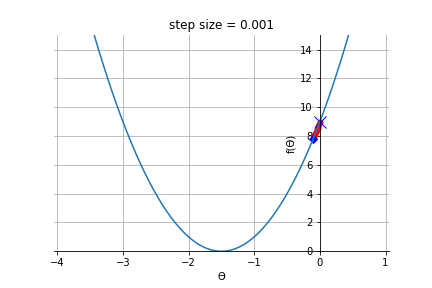
\includegraphics[width=70mm,scale=0.5]{images/gradient_descent_images/converge_slowly.png}
        
        \caption*{Our step size is too small: this is going to take too long!}
        \end{figure}
        
        In-between, it might converge, but \textbf{oscillate} a bunch: this can slow down getting an answer!
        
        \begin{figure}[H]
        \centering
            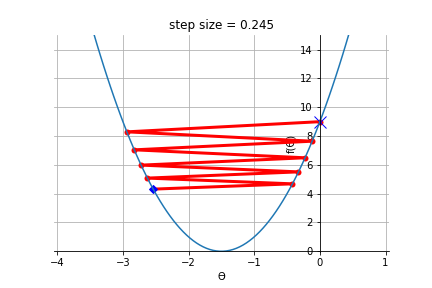
\includegraphics[width=70mm,scale=0.5]{images/gradient_descent_images/oscillate.png}
        
        \caption*{Most of our step is spent undoing the last step... we get better very slowly.}
        \end{figure}
        
        But, if we get the right step size, it'll converge nice and reasonably!
        
        \begin{figure}[H]
            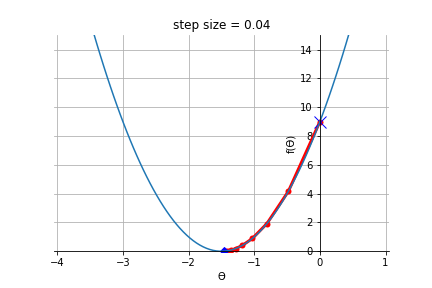
\includegraphics[width=70mm,scale=0.5]{images/gradient_descent_images/good_converge.png}
            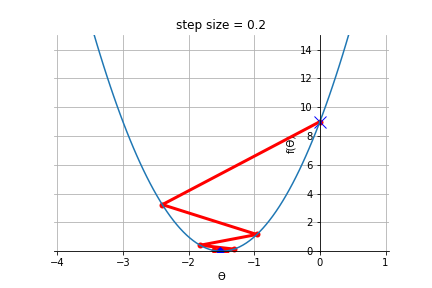
\includegraphics[width=70mm,scale=0.5]{images/gradient_descent_images/good_converge_oscillate.png}

            \caption*{Both of these look pretty good! One of them oscillating a bit is fine.}
        \end{figure}
        
        One question you might ask is, "\textbf{how much} oscillation is too much? Am I converging \textbf{fast enough}?" 
        
        This is a good question, but the simple answer is that there is \textbf{no objective answer}: it depends on what you \textbf{need} and how much \textbf{time} you have. But you should strive to do \textbf{better} when you can!\\
        
        \begin{concept}
            Using the \purp{wrong} step size can cause:
            
            \begin{itemize}
                \item Slow convergence
                \item Strong Oscillation
                \item Divergence
            \end{itemize}
            
            Which is why we \gren{adjust} the step size using $\eta$.
        \end{concept}
        
    \subsection{Step size $\eta$}
    
        Right now, our step size is at the mercy of $J'(\theta)$. But, we don't have to be: we could \textbf{scale} our step size up or down.
        
        We do this with our \textbf{scaling} factor (also called a \textbf{learning rate}), $\eta$.
        
        So, we can rewrite our \textbf{change} in $\theta$ as:
        
        \begin{equation}
            \Delta \theta
            = -\red{\eta}   \deriv{J}{\theta}
            = -\red{\eta}   J'(\theta)
        \end{equation}
        
        \begin{definition}
            Our step size parameter $\eta$, or \vocab{eta}, \purp{scales} how large each of our optimization steps are.
            
            If $\eta$ is bigger, we might \gren{learn} faster, but we also risk \purp{diverging}.
            
            Different values of $\eta$ are good for \gren{different situations}.
        \end{definition}
        
    \subsection{Our procedure}
    
        So, we have our parameter \textbf{update}, $\Delta \theta$. We'll start at $t=0$.
        
        Before, we represented the $\nth{i}$ \textbf{data point} with $\ex{x}{i}$. We'll reuse this \textbf{notation}.\\
        
        \begin{notation}
            Here, we're changing $\theta$ over \purp{time}: each step happens at $t=\{1,2,3, \dots \}$ so we need \gren{notation} for that. 
            
            We'll \gren{reuse} the notation from $\ex{x}{i}$, for the $\nth{i}$ data point.
            
            In this case, we'll do $\ex{\theta}{t}$: the value of $\theta$ after $t$ \purp{steps} are taken.
            
            Earlier, we \textbf{introduced} \blu{$\theta_{old}$} and \red{$\theta_{new}$}: these are \blu{$\ex{\theta}{t-1}$} and \red{$\ex{\theta}{t}$}.
        \end{notation}
        
        \miniex After \textbf{10 steps} of 1-D gradient descent, we have gone from $\ex{\theta}{0}$ to $\ex{\theta}{10}$.
        
        So, we move the \textbf{first} time using $J'(\ex{\theta}{0})$.
        
        Once we've moved in parameter space \textbf{one} time, though, our \textbf{derivative} has changed: we're in a different part of the \textbf{surface}.
        
        So, we'll take a \textbf{second} step with a \textbf{new} derivative, $J'(\ex{\theta}{1})$.
        
        We want to do this \textbf{repeatedly}. We'll take our equation
        
        \begin{equation}
            \theta_{new} = \theta_{old} + \Delta \theta
        \end{equation}
        
        And combine it with our \textbf{chosen} step size.\\
        
        \begin{kequation}
            In \vocab{1-D}, \vocab{Gradient Descent} is implemented as follows:
        
            At each time step $t$, we \purp{improve} our hypothesis $\theta$ using the following rule:
            
            \begin{equation*}
                \red{ \theta_{new} } = 
                \blu{ \theta_{old} } - \grn{\eta} J'( \blu{ \theta_{old} })
            \end{equation*}
            
            Using $\ex{\theta}{t}$ notation:
            
            \begin{equation*}
                \red{ \ex{\theta}{t} } = 
                \blu{ \ex{\theta}{t-1} } -
                \grn{\eta} J'( \blu{ \ex{\theta}{t-1} })
            \end{equation*}
            
            We repeat until we reach whatever our chosen \purp{termination condition} is.
        \end{kequation}
        
        We can also write it as:
        
        \begin{equation*}
                \red{ \theta_{new} } = 
                \blu{ \theta_{old} } - 
                \grn{\eta} 
                \left( \deriv{J}{ \blu{ \theta_{old} }} \right)
            \end{equation*}
        
        We've got our gradient descent \textbf{update} rule in 1-D!
    
    \subsection{Termination Conditions}
    
        When do we \textbf{stop}? We can't let it run forever.
        
        We have some options:
        
        \begin{itemize}
            \item Stop after a \textbf{fixed} $T$ steps.
                \begin{itemize}
                    \item This has the advantage of being \textbf{simple}, but how do you know what the \textbf{correct} number of steps is?
                \end{itemize}
            
            \item Stop when $\theta$ \textbf{isn't changing} much: $\big| \Delta \theta \big| < \epsilon$, for example.
            \begin{itemize}
                \item If our $\theta$ isn't changing much, our algorithm isn't \textbf{improving} our hypothesis much. So, it makes sense to stop: we've stabilized.
            \end{itemize}
            
            \item Stop when the \textbf{derivative is small}: $\big| J'(\theta) \big| < \epsilon$.
            \begin{itemize}
                \item Mathematically \textbf{equivalent} to our last choice. But a different \textbf{perspective}: if the slope is small, our surface is relatively \textbf{flat}, and we're near a \textbf{minimum} (probably).
                
                \item "The derivative is \textbf{small}" is weaker, but in the same spirit as "the derivative is \textbf{zero}", $J'(\theta)=0$, from last chapter.
            \end{itemize}
            
        \end{itemize}
        
    \subsection{Convergence Theorem}
    
        It turns out, if our function is \textbf{nice} enough, and we pick the \textbf{right} value of $\eta$, we can guarantee convergence!\\
        
        \begin{theorem}
            We want to optimize function $J$. If J is 
            \begin{itemize}
                \item Smooth enough
                \item Convex
            \end{itemize}
            
            And
            
            \begin{itemize}
                \item $\eta$ is small enough
            \end{itemize}
            
            Then gradient descent \textbf{will} converge to the \textbf{global minimum}!
        \end{theorem}
        
        "Small enough" seems vague, but it basically means, "an $\eta$ small enough to converge \textbf{exists}". 
            \note{If we want to say it in a mathy way, we can say "\textbf{there exists} an $\eta$ small enough to converge"} 
        
        Or, if your $\eta$ is too \textbf{big}, you can keep trying \textbf{smaller} ones, until it works. 
        
        This is amazing! We can \textbf{guarantee} a best solution in some cases!
        
    \subsection{Concavity}
    
        One requirement we haven't focused on "$J$ is \textbf{convex}". Why do we need $J$ to be convex?
        
        Well, if it's \textbf{concave}, there is no \textbf{global minimum}: it goes down forever!\\
        
        \begin{figure}[H]
        \centering
            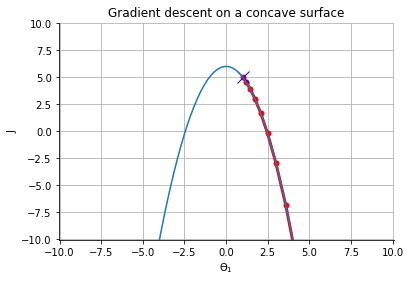
\includegraphics[width=70mm,scale=0.5]{images/gradient_descent_images/gradient_descent_on_a_concave_surface.png}
        
        \caption*{Our gradient just leads us downhill forever.}
        \end{figure}
        
        \begin{concept}
            If our function $J$ is \purp{concave}, then our result will not \purp{converge}: it will continue to \gren{decrease} more and more indefinitely.
        \end{concept}
        
        So, for future problems, let's assume it \textbf{doesn't} go down forever: if it was, then there is no best solution! We don't have a \textbf{valid} problem.
        
    \subsection{Local minima}
        
        Even if we don't have that problem, we have a \textbf{different} one:
        
        Gradient descent \textbf{gradually} improves our solution until it reaches one it's \textbf{satisfied} with. But, what if there are \textbf{multiple} solutions we could reach?
        
        Are they all equally good?
        
        \begin{figure}[H]
        \centering
            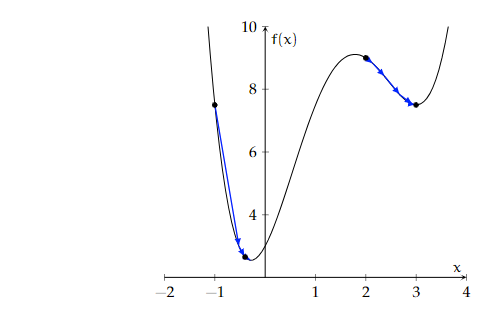
\includegraphics[width=70mm,scale=0.5]{images/gradient_descent_images/Two_Local_Minima.png}
        
        \caption*{Depending on your starting position (\textbf{initialization}), you could find a different local minimum!}
        \end{figure}
        
        Maybe not! So, if our function isn't \textbf{always convex}, we can end up with \textbf{multiple} "valleys", or \textbf{local} minima.\\
        
        \begin{definition}
            A \vocab{global} minimum is the \purp{lowest} point on our entire function: the one with the lowest \gren{output}.
            
            A \vocab{local} minimum is one that is the \gren{lowest} point among those points that are \purp{near} it.
            
            \begin{itemize}
                \item For \vocab{local minima}, if you add or subtract a \purp{small} amount $\epsilon$, the value will \gren{increase}.
            \end{itemize}
            
        \end{definition}
        
        So, we \textbf{won't} necessarily end up with the \textbf{global} minimum, even with a \textit{small} $\eta$.
        
        This shows that \textbf{initialization matters}!\\
        
        \begin{definition}
            \vocab{Initialization} is our "starting point": when we first \gren{start} our algorithm, what are our \purp{parameters} set to?
        \end{definition}
        
        If we have a \textbf{different} starting position, we can find a \textbf{different} local minimum.\\
        
        \begin{concept}
            \vocab{Gradient descent} finds \purp{local} minima near the initialization, not \purp{global} minima.
            
            This means, if our function has \vocab{multiple local minima} (not fully convex), our \vocab{initialization} can affect our \gren{solution}.
        \end{concept}

\pagebreak

%%%%%%%%%%%%%%%%%%%%%%%%%%%%%%%%%%%%%%%%%%%%%%%%%%%%%%%%%%%%%%%%%%%%%%%%%%%%%%%%%%%%%%%%%%%
\section{Multiple Dimensions}

    Now that we've handled the 1-D case, we'll move into 2-D: now, we have \textbf{two} parameters, $\theta_1$ and $\theta_2$, as the input to $J$.
    
    \begin{figure}[H]
        \centering
            \includegraphics[width=70mm,scale=0.5]{images/gradient_descent_images/3dplot.png}
        
        \caption*{The "height"of your plot in 3D, is, again, your output! You want to move \textbf{downhill}.}
    \end{figure}
        
    \subsection{Multivariable Local Approximation (Review)}
    
        Again, we rely on \textbf{calculus}. We want to move up to having more parameters: more \textbf{dimensions}. 
        
        Before, in 1-D, we found that, if you \textbf{zoomed} in enough on a function (using a "\textbf{local} view"), we could \textbf{approximate} it as a \textbf{straight line}, and move up or down that slope.
        
        There are \textbf{two} ways we can \textbf{approximate} like we want to in 2-D:
            \note{Remember that, by 2-D, we mean two \textbf{parameters}/inputs to $J$. If we add in the \textbf{height} of our function, that means our plot will \textbf{look} like 3-D!}
        
        \begin{itemize}
            \item First, we could turn it back into 1-D: we remove one variables.
            
            We do this by turning one variable constant: take $\theta_2=0$. Now, we have one free variable $\theta_1$. Same as 1-D.\\
        \end{itemize}
        
        \begin{concept}
            We can \gren{reduce} the number of \purp{variables} we have to work with, by holding some of them \gren{constant}. That way, we have a \purp{simpler} problem to work with.
            
            This is \purp{the same} as taking a single 2-D plane in a 3-D plot.
        \end{concept}
        
        \begin{figure}[H]
                \includegraphics[width=70mm,scale=0.5]{images/gradient_descent_images/theta2_eq_0_unsliced.png}
                \includegraphics[width=70mm,scale=0.5]{images/gradient_descent_images/theta2_eq_0_sliced.png}
            
            \caption*{If we focus on a single plane of this surface, we end up with a \textbf{parabola}.}
        \end{figure}
        
        We can do the same the other way: we take $\theta_1=0$, and now we have a 1-D problem in $\theta_2$.
        
        \begin{figure}[H]
                \includegraphics[width=70mm,scale=0.5]{images/gradient_descent_images/theta1_eq_0_unsliced.png}
                \includegraphics[width=70mm,scale=0.5]{images/gradient_descent_images/theta1_eq_0_sliced.png}
            
            \caption*{We can slice along the other axis as well!}
        \end{figure}

        Along each \textbf{axis}, $\theta_1$ and $\theta_2$, you can \textbf{approximate} our function as \textbf{two} different straight lines. Which leads into our next point...
        
        \begin{itemize}
            \item Second way: if we take the two perpendicular \textbf{lines} we got from each dimension, we can combine them into a \textbf{plane}.\\
        \end{itemize}
        
        \begin{concept}
            If we have \vocab{two input variables} (a 2-D problem), we can \purp{approximate} our surface as a \vocab{plane} if we \gren{zoom} in enough.
        \end{concept}
        
        These \textbf{approximations} will allow us to \textbf{optimize}.

    \subsection{2-D: One dimension at a time}
        
        How do we \textbf{improve} our function $J$? Now that we have \textbf{two} dimensions, we have to store our change $\Delta \theta$ in a \textbf{vector}:
        
        \begin{equation}
            \Delta \theta
            =
            \begin{bmatrix}
                  \Delta \theta_1 \\ \Delta \theta_2 
            \end{bmatrix}
        \end{equation}
        
        This \textbf{complicates} things: we have two different things to consider \textbf{at once}.
        
        Well, the \textbf{simplest} way would be to treat it as a \textbf{1-D} problem, and do exactly what we did \textbf{before}. 
            \note{Note that we switched to \textbf{partial} derivatives, because we have \textbf{multiple} input variables $\theta_i$.}
        
        \begin{equation}
            \Delta \theta_1 = \pderiv{J}{\theta_1}
        \end{equation}
        
        Writing this in our \textbf{new} notation, we get:
        
        \begin{equation}
            \Delta \theta
            =
            - \eta 
            \begin{bmatrix}
                  \pderivslash{J}{\theta_1} \\ 0 
            \end{bmatrix}
        \end{equation}
        
        And then we would take a \textbf{step}, moving along the $\theta_1$ \textbf{axis}.
        
        \begin{figure}[H]
            \centering
                \includegraphics[width=70mm,scale=0.5]{images/gradient_descent_images/theta1_movement_plane.png}
            \caption*{We can move along $\theta_1$ just like on a line.}
        \end{figure}
        
        What if we treated this as a 1-D problem for the \textbf{other} variable, $\theta_2$?
        
        \begin{equation}
            \Delta \theta
            =
            - \eta 
            \begin{bmatrix}
                  0 \\ \pderivslash{J}{\theta_2} 
            \end{bmatrix}
        \end{equation}
        
        With this equation, we would be \textbf{moving} along the $\theta_2$ axis.
        
        \begin{figure}[H]
            \centering
                \includegraphics[width=70mm,scale=0.5]{images/gradient_descent_images/theta2_movement_plane.png}
            \caption*{We can do the same with $\theta_2$.}
        \end{figure}
        
        Why not move in \textbf{both} directions \textbf{at once}? We can \textbf{combine} our two derivatives: we'll add up our two steps.
        
        \textbf{Linearity} means that I can \textbf{add} them up without anything \textbf{weird} happening.
            \note{The relevant linearity rule: $L(x+y)=L(x)+L(y)$. In other words: taking two separate steps is the same as one big step.}
        
        \begin{equation}
            \Delta \theta
            =
            - \eta 
            \begin{bmatrix}
                  \pderivslash{J}{\theta_1} \\ 0 
            \end{bmatrix}
            - \eta 
            \begin{bmatrix}
                  0 \\ \pderivslash{J}{\theta_2} 
            \end{bmatrix}
        \end{equation}
        
        These can be combined because we're treating our function as a \textbf{flat} plane: if I move in the $\theta_1$ direction first, it doesn't change the $\theta_2$ slope, and vice versa.
        
        \begin{figure}[H]
        \centering
            \includegraphics[width=70mm,scale=0.5]{images/gradient_descent_images/thetaboth_movement_plane.png}

            \includegraphics[width=70mm,scale=0.5]{images/gradient_descent_images/thetaboth_movement_plane_reversed.png}
                
            \caption*{Our plane being flat means we can take both operations, back-to-back! Notice that the order doesn't matter.}
        \end{figure}
        
        \begin{equation}
            \Delta \theta
            =
            - \eta 
            \begin{bmatrix}
                  \pderivslash{J}{\theta_1} \\ \pderivslash{J}{\theta_2} 
            \end{bmatrix}
        \end{equation}
        
        So, let's use that to optimize:\\
        
        \begin{kequation}
            In \vocab{2-D}, you can optimize your function $J$ using this rule:
            
            \begin{equation*}
                \red{ \theta_{new} } =  \blu{ \theta_{old} } 
                - \grn{ \eta } 
                \underbrace{
                    \begin{bmatrix}
                          \pderivslash{J}{ \blu{\theta_1} } \\ 
                          \pderivslash{J}{ \blu{\theta_2} } 
                    \end{bmatrix}
                }_{ \text{Using } \blu{ \theta_{old} } }
            \end{equation*}
            
            This is our \vocab{gradient descent} rule for 2-D.
        \end{kequation}
        
        This sort of approach makes some \textbf{sense}: if $\pderiv{J}{\theta_1}$ is \textbf{bigger} than $\pderiv{J}{\theta_2}$, that means that you can get \textbf{more benefit} from moving in the $\theta_1$ direction than $\theta_2$.
        
        So, in that case, your step will move more in the $\theta_1$ direction: it's a more \textbf{efficient} way to get a \textbf{better} hypothesis!
        
        But for now, we \textbf{don't know} that this is necessarily the \textbf{optimal} way to change $\theta$ - we'll explore that later.
        
        
    \subsection{Gradient Descent in n-D}
    
        This idea can be built up in \textbf{any number} of dimensions: each variable $\theta_k$ creates a \textbf{different} line we can use to \textbf{approximate}.
        
        And, we can combine them into a \textbf{flat} hyperplane: so, we can \textbf{add up} all of the different \textbf{derivatives}.\\
        
        \begin{kequation}
            In \vocab{n-D}, you can optimize your function $J$ using this rule:
            
            \begin{equation*}
                \red{ \theta_{new} } =  \blu{ \theta_{old} } 
                - \grn{ \eta } 
                \underbrace{
                    \begin{bmatrix}
                          \pderivslash{J}{ \blu{\theta_1} } \\ 
                          \pderivslash{J}{ \blu{\theta_2} } \\
                          \vdots \\
                          \pderivslash{J}{ \blu{\theta_d} } \\
                    \end{bmatrix}
                }_{ \text{Using } \blu{ \theta_{old} } }
            \end{equation*}
            
            This is our \vocab{generalized gradient descent} rule.
        \end{kequation}

    \subsection{The Gradient}
    
        We call this \textbf{gradient} descent because that right term \textbf{is} the gradient!\\
        
        \begin{definition}
            
            The gradient can be written as
            
            \begin{equation*}
                \nabla_\theta J 
                = 
                \begin{bmatrix}
                      \pderivslash{J}{ \blu{\theta_1} } \\ 
                      \pderivslash{J}{ \blu{\theta_2} } \\
                      \vdots \\
                      \pderivslash{J}{ \blu{\theta_d} } \\
                \end{bmatrix}
                =
                \deriv{J}{\theta}
            \end{equation*} 
        \end{definition}
        
        So, our rule can be rewritten (for the last time) as:\\
        
        \begin{kequation}
            The \vocab{gradient descent} rule can be generally written as:
            
            \begin{equation*}
                \red{ \theta_{new} } =  \blu{ \theta_{old} } 
                - \grn{ \eta } 
                \nabla_\theta J ( \blu{ \theta_{old} } )
            \end{equation*}
            
            $\blu{ \theta_{old} }$ is the input to $\nabla_\theta J$, not multiplication!
            
            \begin{equation*}
                \red{ \theta_{new} } =  \blu{ \theta_{old} } 
                - \grn{ \eta } 
                J'( \blu{ \theta_{old} } )
            \end{equation*}
        \end{kequation}
        
        Now, is $\nabla_\theta J$ the \textbf{optimal} way to improve(optimize) $\theta$? Let's find out.
    
    \subsection{The Plane Approximation}
        
        So, what \textbf{is} the best direction? Which way will increase/decrease $J$ \textbf{fastest?} 
        
        \textit{Is} it the gradient? Let's explore a bit to figure that out. Let's look at our plane, and see what hints it might provide:
            \note{For explanation purposes, we'll assume 2-D, but the explanation extends to n-D.}\\
        
        \begin{concept}
            Assume your function is, at least locally, a \vocab{flat plane}.

            \begin{itemize}
                \item A \purp{flat plane} has only \gren{one} direction of \vocab{maximum increase}: this is the direction you might call, "directly \gren{uphill}" if you think of elevation.
                
                \item The \gren{opposite} direction is the direction of \purp{maximum decrease}, or "\gren{downhill}".
                
                \item If you move at a \vocab{right angle} to the "best" direction (maximum increase/decrease), the function \purp{will not change}. In elevation, you stay at the \gren{same height}!
            \end{itemize}
        \end{concept}
        
        This is useful! We can \textbf{break down} any direction into the part that \textbf{affects} our function $J$, and the part that \textbf{doesn't}.
            \note{In the n-D case, we have \textbf{more} perpendicular directions. But, all of them have \textbf{no effect}!}
        
        
    
    \subsection{The Optimal Direction: The Gradient}
    
        How do we get the optimal direction?
        
        The \textbf{total} change in $J$ is gotten by just \textbf{adding} the change in each direction (thank you planes!):
        
        \begin{figure}[H]
        
                \includegraphics[width=70mm,scale=0.5]{images/gradient_descent_images/first_step.png}
                
                \includegraphics[width=70mm,scale=0.5]{images/gradient_descent_images/second_step.png}
                
            \caption*{You can add up the results of our two steps: $\Delta J_2$ and $\Delta J_1$.}
        \end{figure}
        
        \begin{equation}
            \Delta J \approx \Delta J_1 + \Delta J_2
        \end{equation}
        
        Let's convert that using derivatives:
        
        \begin{equation}
            \Delta J \approx
            \Delta \theta_1 \pderiv{J}{\theta_1} +
            \Delta \theta_2 \pderiv{J}{\theta_2}
        \end{equation}
        
        Now we've got a useful equation: the total change. As a bonus we can see a clear \textbf{pattern} ($\nth{i}$ $\theta$ matches $\nth{i}$ derivative). 
        
        So, \textbf{condense} this pattern, like we did for our linear model: using a \textbf{dot product}.
        
        \begin{equation}
            \Delta J 
            \approx 
            \begin{bmatrix}
              \Delta \theta_1 \\ \Delta \theta_2
            \end{bmatrix}
            \cdot
            \begin{bmatrix}
                \pderivslash{J}{ \theta_1}  \\ 
                \pderivslash{J}{ \theta_2 } 
            \end{bmatrix}
            =
            \Delta \theta \cdot \nabla_\theta J
        \end{equation}
        
        The \textbf{gradient} shows up! Interesting. But what does that \textbf{mean}?
        
        Well, we want to \textbf{maximize} (or minimize!) our $\Delta J$. How do we maximize a \textbf{dot product}?
        
        By making sure the directions are \textbf{the same}! So, we can confirm that the \textbf{gradient} gives us the \textbf{best} direction.
        
        So, all we have to do is to \textbf{flip} the sign to \textbf{minimize} $\Delta J$.
            \note{And so, gradient descent is already complete!}\\
        
        \begin{concept}
            The \vocab{gradient} $\nabla J$ is the \vocab{direction of greatest increase} for $J$.
            
            That means means the opposite direction $-\nabla J$ is the \vocab{direction of greatest decrease} in $J$.
        \end{concept}
        
        This is the single \textbf{most important concept} in this entire chapter!
        
        
    \subsection{Termination Condition}
    
        We can still use our termination conditions from before, but we need to be careful to make sure they extrapolate to n-D.
        
        \begin{itemize}
            \item Stop after a fixed T steps.
                \begin{itemize}
                    \item Nothing to change here. 
                        \note{We don't use this one often, though!}
                \end{itemize}
                
            \item Stop when $\norm{\theta}$ isn't changing much: $\norm{\Delta \theta} < \epsilon$, for example.
                \begin{itemize}
                    \item We just had to replace \textbf{absolute} value with \textbf{magnitude}.
                \end{itemize}
                
            \item Stop when the derivative is small: $\abs{J'(\theta)} < \epsilon$
            
                \begin{itemize}
                    \item Nothing to change here.
                \end{itemize}
        \end{itemize}

    \subsection{Another explanation of gradient (OPTIONAL)}
    
        Some students may not like the \textbf{first} explanation given for why gradient is the \textbf{direction of greatest increase}. So here, we use a slightly \textbf{different} approach, one that's more \textbf{geometric}. 
        
        Feel free to skip this section if you are not interested.
        
        We look at a random vector, $\Delta \theta$ - no assurances about how good or bad it is.
        
        Currently, our vector \textbf{components} are based on $\theta_1$ and $\theta_2$. But, we want to \textbf{switch} perspectives.
        
        Our vector can \textbf{also} be broken up into \textbf{parts} based on whether it \textbf{affects} $J$. This will let us take a \textbf{look} at the "best direction" we're trying to \textbf{find}.
        
        \begin{itemize}
            \item Uphill: the "best" direction $\hat{u}_{best}$ (magnitude $\Delta B$)
            
            \item Same height: the direction with no effect, $\hat{u}_{none}$ (magnitude $\Delta N$)
        \end{itemize}
        
        \begin{equation}
            \Delta \theta
            =
            \underbrace{
                \Delta B \red{ \hat{u}_{best} }
            }_{\text{Full effect on J}} 
            + 
            \underbrace{
                \Delta N \red{ \hat{u}_{none} }
            }_{ \text{No effect on J} } 
        \end{equation}
        
        So, all of the change in $J$ just comes from $\hat{u}_{best}$. We \textbf{don't care} about the other direction!\\
        
        \begin{concept}
            In a \vocab{local planar approximation}, the \purp{only} component of $\Delta \theta$ that \gren{affects} $J$ is the \vocab{direction of greatest increase}, $\hat{u}_{best}$.
            
            So, we can determine $\Delta J$ using \purp{only that component}.
        \end{concept}
        
        But, $\nabla_{\theta} J$ \textbf{also} gives us change in $\Delta J$: it contains all of the \textbf{derivatives}, and thus gives us the effect $\theta$ has on $\Delta J$.
        
        So we can find:
        
        \begin{equation}
            \Delta \theta \cdot \deriv{J}{\theta} 
            = \Delta J = 
            \left( 
                \Delta \theta \cdot \hat{u}_{best} 
            \right) 
            \deriv{J}{B}
        \end{equation}
        
        $\Delta \theta$ is being dotted with both the \textbf{gradient} and the \textbf{best direction}: they both give the change in $J$. To keep the \textbf{dot product} consistent as $\Delta \theta$ changes, they need to be in the \textbf{same direction}.

\pagebreak
%%%%%%%%%%%%%%%%%%%%%%%%%%%%%%%%%%%%%%%%%%%%%%%%%%%%%%%%%%%%%%%%%%%%%%%%%%%%%%%%%%%%%%%%%%%
\section{Application to Regression}
    
    One nice thing about \textbf{gradient descent} is that it is \textbf{easy} to switch the kind of problem you're applying it to: all you need is your \textbf{parameters}(s) $\theta$, and a function to optimize, $J$.
    
    From there, you can just \textbf{compute} the gradient.

    \subsection{Ordinary Least Squares}
        
        Our \textbf{loss} function is
        
        \begin{equation}
            J(\theta,\theta_0) = 
            \frac{1}{n}  \sum_{i=1}^n 
            \left( \red{ (\theta^T} \blu{\ex{x}{i}} \red{ + \theta_0) } 
            - \blu{\ex{y}{i}} \right)^2 
        \end{equation}
            
        Or, in \textbf{matrix} terms,
            \note{Including the appended row of 1's from before.}
        
        \begin{equation*}
            J = \frac{1}{n}
                \left( \red{ \Xt \theta  - \Yt } \right)^T
                \left( \red{ \Xt \theta  - \Yt } \right) 
        \end{equation*}
        
        Our gradient, according to \textbf{matrix derivative} rules, is
        
        \begin{equation}
            \nabla_\theta J(\theta) = 
                \frac{2}{n} \Xt^T
                \left( \red{ \Xt \theta  - \Yt } \right) 
        \end{equation}
        
        Before, we set it equal to \textbf{zero}. But here, we can instead take \textbf{steps} towards the solution, using \textbf{gradient descent}.
        
        We could use the \textbf{matrix} form, but sometimes it's easier to use a \textbf{sum}. Fortunately, derivatives are easy with a sum. If so, here's \textbf{another} way to write it:
        
        \begin{equation}
            \nabla_\theta J(\theta) 
            = 
            \frac{2}{n} \sum_{i=1}^n
            \left(
                \red{\theta^T} \blu{\ex{x}{i}} - \blu{\ex{y}{i}}
            \right)
            \blu{\ex{x}{i}}
        \end{equation}
        
        Either way, we use gradient descent \textbf{normally}:
            \note{Remember that $\blu{ \theta_{old} }$ is an \textbf{input} to the gradient, not multiplied by it!}
        
        \begin{equation*}
            \red{ \theta_{new} } 
            =  
            \blu{ \theta_{old} } 
            - \grn{ \eta } 
            \nabla_\theta J ( \blu{ \theta_{old} } )
        \end{equation*}
        
        Using $\ex{\theta}{t}$ notation:
        
        \begin{equation*}
            \red{ \ex{\theta}{t} } = 
            \blu{ \ex{\theta}{t-1} } -
            \grn{\eta} \nabla_\theta J ( \blu{ \ex{\theta}{t-1} })
        \end{equation*}
        
    \subsection{Ridge Regression}
    
        Ridge regression is similar. 
        
        \begin{equation*}
                J(\theta) 
                = 
                \frac{1}{n}  \sum_{i=1}^n 
                \left( 
                    \underbrace{
                        \red{(\theta^T \ex{x}{i}  
                        + \theta_0)}
                    }_{guess}
                    - \underbrace{
                        \blu{\ex{y}{i}} 
                    }_{answer}
                \right)^2 
                + 
                \underbrace{
                    \pur{ \lambda \norm{\theta}^2 }
                }_{Regularizer}
            \end{equation*}
        
        However, we have to treat $\theta_0$ as \textbf{separate} from our other data points, because of \textbf{regularization}: remember that it \textbf{doesn't} apply to $\theta_0$.
        
        For $\theta$:
        
        \begin{equation}
            \nabla_\theta J_\text{ridge}(\theta, \theta_0)
            =
            \frac{2}{n}\sum_{i=1}^n
            \left(
                \red{(\theta^T} \blu{\ex{x}{i}} + \red{\theta_0)}
                - 
                \blu{\ex{y}{i}}
            \right)
            \blu{\ex{x}{i}}
            +
            \pur{2 \lambda \theta}
        \end{equation}
        
        For $\theta_0$:
        
        \begin{equation}
            \pderiv{J_\text{ridge}(\theta, \theta_0)}{\theta_0} 
            =
            \frac{2}{n}\sum_{i=1}^n
            \left(
                \red{(\theta^T} \blu{\ex{x}{i}} + \red{\theta_0)}
                - 
                \blu{\ex{y}{i}}
            \right)
        \end{equation}
        
        Notice that we used a \textbf{gradient} for our vector $\theta$, but since $\theta_0$ is a single variable, we just used a \textbf{simple derivative}!\\
        
        \begin{concept}
            The \vocab{gradient} $\deriv{J}{\theta}$ must have the \vocab{same shape as $\theta$}: this shape-matching is why we can easily \gren{subtract} it during gradient descent.
            
            \begin{equation*}
                \underbrace{
                    \red{ \theta_{new} } 
                }_{(d \times 1)}
                =  
                \underbrace{
                    \blu{ \theta_{old} } 
                }_{(d \times 1)}
                - \grn{ \eta } 
                \underbrace{
                    \nabla_\theta J ( \blu{ \theta_{old} } )
                }_{(d \times 1)}
            \end{equation*}
        \end{concept}
    
    \subsection{Computational Gradient}
    
        Sometimes, we \textbf{can't} easily find the \textbf{equation} for our gradient: maybe our loss isn't a simple \textbf{equation}, or we have some \textbf{other} kind of problem. So, rather than getting the \textbf{exact} gradient, we \textbf{approximate} it.
        
        But how do we \textbf{approximate} the gradient? Well, first, we could \textbf{reference} how we approximate a \textbf{simple derivative}.
            \note{A derivative is just a 1-D gradient, after all!}
            
        The definition of the \textbf{derivative} can be gotten as 
        
        \begin{equation}
            f'(x) = \lim_{h \rightarrow 0} \frac{f(x+h)-f(x)}{h}
        \end{equation}
        
        But, what if we can't take the \textbf{limit}? Or, we just don't \textbf{want} to? 
        
        We can \textbf{approximate} by taking $h$ to be a small, \textbf{finite} number.
        
        Instead of $h$, we'll call this $\delta$.
        
        \begin{concept}
            When \vocab{approximating} the derivative, we can choose a \purp{small} finite width to measure, called $\delta$, so that
            
            \begin{equation}
                \deriv{f}{x} \approx
                \frac{f(x+\delta)-f(x)}{\delta} , \qquad \delta << 1
            \end{equation}
        \end{concept}
        
        So, let's \textbf{extend} that to the \textbf{gradient}:
        
        \begin{equation}
            \nabla_\theta J 
            = 
            \begin{bmatrix}
                  \pderivslash{J}{ \blu{\theta_1} } \\ 
                  \pderivslash{J}{ \blu{\theta_2} } \\
                  \vdots \\
                  \pderivslash{J}{ \blu{\theta_d} } \\
            \end{bmatrix}
        \end{equation}
        
        Luckily, the \textbf{gradient} is just a bunch of derivatives \textbf{stacked} in a \textbf{vector}! 
        
        So, we can just \textbf{compute} each of them \textbf{separately}, and then put them together.
        
        Let's show how we'd \textbf{write} that in \textbf{vector} form, for just one of them. We want something like
        
        \begin{equation}
            \underbrace{
                J'(\theta) \approx
                \frac{J(\theta+\delta)-f(\theta)}{\delta} 
            }_{\text{Not correct, but closer}}
        \end{equation}
        
        This isn't quite right, because a \textbf{scalar} $\delta$ would \textbf{add} to \textbf{every term}.
        
        We \textbf{only} want to shift \textbf{one} variable at a time, so we can do a \textbf{simple} derivative.
        
        Let's say we want $\derivslash{J}{\theta_1}$. We would \textbf{only} want to add $\delta$ to $\theta_1$: the other parameters are \textbf{unchanged}.
        
        So, we \textbf{can't} add a \textbf{scalar}. Instead, we need a $(d \times 1)$ vector: one term to \textbf{separately} add to each $\theta_k$ term.
        
        \begin{equation}
            \Delta \theta 
            = 
            \begin{bmatrix}
                \Delta \theta_1 \\ \Delta \theta_2 \\ \vdots \\ \Delta \theta_d
            \end{bmatrix}
        \end{equation}
        
        We want most terms \textbf{unchanged}, so we'll \textbf{add 0} to each of them, and we'll add $\delta$ to the one term we want to \textbf{edit}.
        
        \begin{equation}
            \Delta \theta 
            = 
            \begin{bmatrix}
                \delta \\ 0 \\ \vdots\\ 0 \\ 0
            \end{bmatrix}
        \end{equation}
        
        We'll \textbf{create} one of these vectors for each \textbf{dimension}. We'll give them a special \textbf{name}: $\delta_k$, for the $\nth{k}$ dimension.
        
        \begin{equation}
            \delta_1 
            = 
            \begin{bmatrix}
                \delta \\ 0 \\ \vdots\\ 0 \\ 0
            \end{bmatrix}
            \qquad
            \delta_2 
            = 
            \begin{bmatrix}
                0 \\ \delta \\ \vdots\\ 0 \\ 0
            \end{bmatrix}
            \qquad
            \delta_{d-1} 
            = 
            \begin{bmatrix}
                0 \\ 0 \\ \vdots\\ \delta \\ 0
            \end{bmatrix}
            \qquad
            \delta_{d} 
            = 
            \begin{bmatrix}
                0 \\ 0 \\ \vdots\\ 0 \\ \delta
            \end{bmatrix}
        \end{equation}
        
        Finally, we'll \textbf{divide} by $\delta$. We have what we need for our full equation:\\
        
        \begin{kequation}
            In order to \vocab{computationally find the gradient}, you need to find the \purp{partial derivative} for each term $\theta_k$.
            
            \begin{equation*}
                \deriv{J}{\theta_k} \approx
                \frac{J(\theta+\delta_k)-f(\theta)}{\delta}
            \end{equation*}
            
            Where 
            
            \begin{itemize}
                \item $\delta$ is a small positive number
                \item $\delta_k$ is the $(d \times 1)$ \gren{column vector} with a $\delta$ in the $\nth{k}$ row, and a 0 in every other row.
            \end{itemize} 
        \end{kequation}

    
    \subsection{Problems with Gradient Descent}
        
        Gradient descent is very handy, but it's important to be aware of some of its \textbf{problems}.
        
        We've discussed a couple: diverging, oscillating, and converging slowly. We also have to worry about \textbf{local minima} that aren't as good as other answers.
        
        But there's also a \textbf{limitation}: our loss function has to be \textbf{smooth} and \textbf{differentiable}. If it isn't, we can't take the \textbf{gradient} of it.\\
        
        \begin{concept}
            \vocab{Gradient descent} requires for your \gren{functions} to be (at least mostly) \vocab{smooth and differentiable.}
        \end{concept}
        
        Our \textbf{answer} is also only as good as our \textbf{loss function}: if our loss function is not good for what we actually want to \textbf{accomplish}, then we can easily create a \textbf{bad} model.
        
\pagebreak
%%%%%%%%%%%%%%%%%%%%%%%%%%%%%%%%%%%%%%%%%%%%%%%%%%%%%%%%%%%%%%%%%%%%%%%%%%%%%%%%%%%%%%%%%%%
\section{Stochastic Gradient Descent}

    \subsection{Another problem with gradient descent}
        One \textbf{advantage} we mentioned for gradient descent at the beginning of the chapter is that we can \textbf{stop early} if we think we're done, saving on \textbf{time}.
        
        This is helpful for really \textbf{large} datasets, and it's also more \textbf{computationally manageable} than inverting a gigantic $XX^T$ matrix.
        
        But, we \textbf{haven't} taken \textbf{full advantage} of it: above, we used a \textbf{sum} to get our gradient - we're assuming we'll use all of our \textbf{data points}.
        
        But, what if we don't want to have to use all of them at once? That might be \textbf{expensive}. 
        
        And in fact, there are \textbf{other} reasons not to: maybe the gradient will change directions after only a \textbf{small} distance. 
        
        Right now, we're getting \textbf{lots of data} before even taking a \textbf{single step}: if we start moving \textbf{immediately}, our program could \textbf{adapt} to the "terrain" more quickly!
        
    \subsection{A better way: stochastic GD}
        
        Instead, why wait until we have \textbf{added} up over all the data? We could just \textbf{compute} the gradient over \textbf{one} data point \textbf{at a time}. In fact, to be fair, we'll do it \textbf{randomly}. 
            \note{To compensate, our steps will have to be \textbf{smaller}!}
        
        But wait, this \textbf{seems} like it would be \textbf{less} effective - after all, how much does \textbf{one} data point tell you? 
        
        Well, even if it isn't much, this isn't very \textbf{different} from adding them up all at \textbf{once}: in \textbf{theory}, taking lots of \textbf{little} steps should average out to the \textbf{same} information as if we do it all at once.\\
        
        \begin{definition}
            \vocab{Stochastic Gradient Descent (SGD)} is the process of applying \purp{gradient descent} on \gren{randomly} selected data points.
            
            This should \gren{average} out to being \gren{similar} to regular (batch) gradient descent, but the \purp{randomness} often lets it improve \purp{faster} and \gren{avoid} some common problems.
        \end{definition}
            
        \note{Stochastic is just a very mathematically precise word for "random".}
        
        There are more possible benefits, too: \textbf{randomly} choosing data points adds some \textbf{noise}, and random movement might be able to pull us out of local minima we don't want.
            \note{We mean "noise" in the signals sense: random \textbf{variation} in our data that \textbf{isn't} part of what we're trying to pay attention to: in this case, the \textbf{distribution}.}
            
        This sort of \textbf{noise} and \textbf{randomness} can make it hard for our model to \textbf{perfectly} fit the training data: this can reduce \textbf{overfitting}, too!
            \note{For example, it's hard to focus on the details of someone's eyelashes (unimportant details) if your vision is blurry.}
            
        \begin{concept}
            There are many \vocab{benefits} to \vocab{SGD} (Stochastic Gradient Descent) over regular BGD (Batch Gradient Descent).
            
            \begin{itemize}
                \item SGD can sometimes \gren{learn} a good model \purp{without} using all of our \gren{data}, which can \vocab{save us time} when data sets are \purp{too large}.
                    \begin{itemize}
                        \item It can also let us address problems \gren{early} if the model \purp{isn't} improving.
                    \end{itemize}
                    
                \item The noise produced by the random sampling in SGD can sometimes help it \vocab{avoid local minima} that aren't very good models, 
                    \begin{itemize}
                        \item This is because the model might be moved in a \purp{random direction} in \gren{parameter space}, and randomly \gren{pulled out} of that minimum, even if BGD would have gotten \purp{stuck}.
                    \end{itemize}
                    
                \item The noise also \vocab{reduces overfitting}, because it's \gren{harder} for the model to \purp{memorize} the exact details of the \purp{distribution}.
            \end{itemize}
        \end{concept}
        
    \subsection{Ensuring Convergence}
    
        How do we make sure that our SGD method converges? We need some kind of termination criteria. Thankfully, there's a useful theorem on the matter:\\
        
        \begin{theorem}
            SGD \purp{converges} with \textit{probability one} to the \purp{optimal} $\Theta$ if
            
            \begin{itemize}
                \item $f$ is convex
            \end{itemize}
            
            And our step size(learning rule) $\eta(t)$ follows these rules:
            
            \begin{equation*}
                \sum_{t=1}^{\infty} \eta(t) = \infty
                \qquad \qquad
                and
                \qquad \qquad
                \sum_{t=1}^{\infty} \eta(t)^2 < \infty
            \end{equation*}
        \end{theorem}
        
        Why these rules? Let's see:
        
        \begin{itemize}
            \item The \textbf{first} rule is for the \textbf{same} reason as for regular BGD: if it isn't \textbf{convex}, we can get stuck in \textbf{local minima}, or if it's \textbf{concave}, decrease \textbf{forever}.
            
            \item The \textbf{second} rule means that your steps need to add up to an \textbf{infinite distance}: this allows you to reach \textbf{any} possible point in your \textbf{parameter space}.
            
            \item The \textbf{third} one is a bit \textbf{trickier}, but basically means the steps need to get \textbf{smaller}, so we can approach the \textbf{minimum} (otherwise we might \textbf{diverge}!)
        \end{itemize}
        
        One option is $\eta(t)=1/t$. But often, we use rules that \textbf{decrease} more \textbf{slowly}, so that it doesn't take as \textbf{long}.
            \note{But technically, we're no longer guaranteed convergence!}

\section{Terms}
    
    \begin{itemize}
        \item Gradient Descent
        \item Parameter Space
        \item Local view (Calculus)
        \item Linear Function Approximation
        \item Planar Function Approximations
        \item Convergence
        \item Divergence
        \item Oscillation
        \item Step size
        \item Termination Condition
        \item Concavity/Convexity
        \item Global Minimum
        \item Local Minimum
        \item Initialization
        \item Gradient (Direction of Maximum Increase)
        \item Gradient Descent Rule
        \item Gradient Shape
        \item Gradient Approximation
        \item Stochastic Gradient Descent
        \item Batch Gradient Descent
        \item BGD Convergence Theorem
        \item SGD Convergence Theorem
    \end{itemize}
% \setcounter{chapter}{3}

\chapter{Classification}

    \subsection{Regression (Review)}
    
        In chapter 2, we handled the problem of \textbf{Regression}: taking in lots of data (stored as a \textbf{vector of real numbers}), and returning another single \textbf{real number}.
            \note{Remember that we used a $(d \times 1)$ column vector for our data points $\ex{x}{i}$.}
        
        \begin{equation}
            h_{reg}: \RR^d \rightarrow \RR
        \end{equation}
        
        This was good for when we wanted to predict some \textbf{numeric} output: stock prices, height, life expectancy, and so on.
        
        But, this isn't the \textbf{only} type of problem we might have to deal with.

\section{Classification}

    \subsection{Motivation: Putting things into classes}
        
        We don't \textit{always} want a \textbf{real number} output: that can be complicated, or not match some problems well. 
        
        Often, it's more useful to, rather than give exact values, sort things into \textbf{categories}, or what we will call \textbf{classes}.\\
        
        \begin{definition}
            A \vocab{class} is \gren{set} of things that have something relevant in \purp{common}.
        \end{definition}
        
        \miniex A beagle and a golden retriever could both be put in a \textbf{class} called "\textbf{dog}". This is useful if you just want to know whether you have a dog or not!
        
    \subsection{What is classification?}
        
        This is the goal of \textbf{classification}: we want to take lots of \textbf{information}, and use them to \textbf{predict} what \textbf{class} a data point belongs in.\\
        
        \begin{definition}
            \vocab{Classification} is the \gren{machine learning problem} of sorting items into different, \purp{discrete} classes.
            
            In this setting, we take \gren{real-valued data}, stored in a $(d \times 1)$ \textbf{vector}, and return one of our \purp{classes}.
            
            \begin{equation*}
                h: \RR^d \rightarrow \{C_1, C_2, C_3, \dots C_n\}
            \end{equation*}
            
            Where $\{C_1, C_2, C_3, \dots C_n\}$ are all \purp{classes}. Sometimes, we call the value we return a \purp{label} instead.
        \end{definition}
        
            \note{As a refresher, the function notation here just says, "take in a $d$-dimensional vector, and output one of our $n$ discrete classes."}
        
        \miniex You might classify different \textbf{animals} as a bird, a mammal, or a fish. You have 5 pieces of useful data to \textbf{classify} with.
        
        \begin{equation}
            h: \RR^5 \rightarrow \{ Bird, Mammal, Fish \}
        \end{equation}
        
                \textbf{Classification} can be useful for lots of situations:

        \begin{itemize}
            \item \textbf{Deciding} which \textbf{action} to take in a difficult situation
            
            \item \textbf{Diagnosing} a patient, and determining the best \textbf{treatment}
            
            \item \textbf{Sort} information to be \textbf{processed} later
            \item And more!\\
        \end{itemize}
        
        Just like with regression, we can depict our \textbf{hypothesis} as the function
        
        \begin{equation}
             x \rightarrow \boxed{h} \rightarrow y 
        \end{equation}

        \begin{concept}
            \vocab{Classification} is also \vocab{supervised}: meaning, you have \purp{training} data $\data_n$ with the \gren{correct} answers given:
            
            \begin{equation*}
                \data_n = 
                \left\{
                    \left(  \ex{x}{1}, \ex{y}{1}    \right), 
                    \dots, 
                    \left(  \ex{x}{n}, \ex{y}{n}    \right)
                \right\}
            \end{equation*}
        \end{concept}
        
            \note{In \textbf{unsupervised} problems, you're not told the "correct" answer and have to just guess one!}
        
    \subsection{Important Facts about Classes}
    
        There's a few important things we should remember about classes moving forward.
        
        \begin{itemize}
            \item Classes are \textbf{discrete}: each class is a distinct "thing", \textbf{separate} from other classes.
            
                \begin{itemize}
                    \item This is unlike real numbers, which are \textbf{continuous}: you can \textbf{smoothly} transition between them.
                \end{itemize}
            
            \item This isn't \textbf{always} true, but usually, classes are \textbf{finite}: there are only so many of them, which we write as $n$.
            
                \begin{itemize}
                    \item Meanwhile, there are \textbf{infinitely many} real numbers.
                \end{itemize}
            
            \item These classes may not have a natural \textbf{order}: is there a correct way to order "$\{ Bird, Mammal, Fish \}$"? Not really.
            
                \begin{itemize}
                    \item The real numbers are ordered, too.
                \end{itemize}
                
            \item In some problems, you get to \textbf{decide} what classes are acceptable: where do you draw the \textbf{line} between two categories? Do you care about dogs, or just mammals? And so on.
            
                \begin{itemize}
                    \item You can change units, but the \textbf{structure} of the real numbers is very \textbf{consistent}.\\
                \end{itemize}
        \end{itemize}
        
        \begin{concept}
            \vocab{Classes} are 
            \begin{itemize}
                \item \gren{discrete}
                \item \gren{finite} (usually)
                \item \gren{not} necessarily \gren{ordered}
                \item often \purp{defined} based on your \purp{needs}
            \end{itemize}
        \end{concept}
        
    \subsection{Binary Classification}
    
        So, how do we get \textbf{started}? Well, we want to create the \textbf{simplest} case, and maybe we can get the \textbf{general} idea.
        
        \textbf{Two} is the \textbf{smallest} number of useful classes: often, this boils down to a \textbf{yes-or-no} question. Typically, we \textbf{represent} these two choices as $+1$ and $-1$, respectively.\\
        
        \begin{definition}
            \vocab{Binary classification} is the \gren{problem} of sorting elements into one of \purp{two categories}. Often, these categories are defined by a "\purp{yes-or-no}" question.
            
            \begin{equation*}
                h: \RR^d \rightarrow \{-1,+1\}
            \end{equation*}
        \end{definition}
        
        \miniex You could look at a person and say, "are they sick?" or, "is that a dog"? You can \textbf{classify} data in a binary way \textbf{based} on those questions.
        
    \subsection{Classification Performance}
        
        And how do we measure how well this model is doing? The easiest way might be, "count the number of wrong guesses".
        
        This is captured by \textbf{0-1 Loss}:\\
        
        \begin{definition}
            \vocab{0-1 Loss} is a way of measuring \gren{classification} performance: if you get the \purp{wrong} answer, you get a loss of \gren{1}. If you're \purp{right}, then \gren{0} loss. 
            
            \begin{equation*}
                \loss(g, a) = 
                \begin{cases}
                     0 & \text{if $g = a$} \\
                     1 & \text{otherwise}
                \end{cases}
            \end{equation*}
        \end{definition}
        
        This type of loss is as \textbf{simple} as we can get: similar to counting how many wrong answers you get on a \textbf{multiple-choice} test.
        
        If we want to get our training error, we'll just average over the data points:
        
        \begin{equation*}
            \trainerr(h) = 
            \red{
                \frac{1}{n} \sum_{i=1}^n
            }
            \begin{cases}
                 0 & \text{if $g = a$} \\
                 1 & \text{otherwise}
            \end{cases}
        \end{equation*}
        
        Just like before, we care about \textbf{testing loss} more than \textbf{training loss}: we want our model to \textbf{generalize}.
            \note{This relies on our typical IID assumption from chapter 1.}
        
        \begin{equation*}
            \testerr(h) = 
            \frac{1}{m} \sum_{i=\red{n+1} }^ {\red{n+m} }
            \begin{cases}
                 0 & \text{if $g = a$} \\
                 1 & \text{otherwise}
            \end{cases}
        \end{equation*}
        
        Next, we figure out what \textbf{model} we use to do our classification.
        
\pagebreak
%%%%%%%%%%%%%%%%%%%%%%%%%%%%%%%%%%%%%%%%%%%%%%%%%%%%%%%%%%%%%%%%%%%%%%%%%%%%%

\section{Linear Classifiers}

    If you wanted to break up your data into two parts ($+1$ and $-1$), how might you do it? Let's explore that question.
    
    \subsection{1-D Linear Classifiers}
    
        As usual, we'll start with the \textbf{simplest} case we can think of: 1-D. So, we only have one variable $x_1$ to \textbf{classify} with.
        
        The simplest version might be to just \textbf{split} our space in \textbf{half}: those above or below a certain \textbf{value}. This is our parameter, $C$.
        
        \begin{equation}
            x_1 > C \qquad \text{or} \qquad x_1 - C > 0
        \end{equation}
        
        \miniex For the below data (where green gives positive and red gives positive), could classify positive as $x_1>3$.
        
        \begin{figure}[H]
            \centering
            \includegraphics[width=70mm,scale=0.4]{images/classification_images/x1_1d_plot_points.png}

            \includegraphics[width=70mm,scale=0.4]{images/classification_images/x1_1d_plot.png}
            
            \caption*{We plot everything above $x=3$ as \textbf{positive}, and \textbf{negative} otherwise.}
        \end{figure}
        
        We could also call it $\theta_0$, in the spirit of our $\theta$ notation for parameters.
        
        \begin{equation}
            x_1 + \theta_0 > 0
        \end{equation}
    
    \subsection{1-D classifiers in 2-D}
        
        Let's add a variable and see how our classifier looks on a 2-D plot.
            \note{We'll omit the data points for now.}
        
        \begin{figure}[H]
                \includegraphics[width=70mm,scale=0.5]{images/classification_images/x1_2d_plot.png}
                \includegraphics[width=70mm,scale=0.5]{images/classification_images/x1_2d_plot_boundary.png}
                
                \caption*{On the right, we've drawn the \textbf{dividing} line between our two regions.}
        \end{figure}
        
        Interesting - the \textbf{boundary} between positive and negative is defined by a \textbf{vertical line}.
        
        Or, almost. Compare $x_1>3$ and $x_1<3$:
        
        \begin{figure}[H]
                \includegraphics[width=70mm,scale=0.5]{images/classification_images/x1_2d_plot_boundary.png}
                \includegraphics[width=70mm,scale=0.5]{images/classification_images/x1_2d_plot_boundary_reversed.png}
                
                \caption*{These two plots have the same line, but have their sides flipped.}
        \end{figure}
        
        So, we have a \textbf{line} that gives us the boundary, but we \textbf{also} need to include information about which way is the \textbf{positive} direction.
        
        What tool best represents \textbf{direction}? We could use angles, but we haven't used that much so far. Instead, let's use a \textbf{vector} to \textbf{point} in the right direction.
        
        \begin{figure}[H]
                \includegraphics[width=70mm,scale=0.5]{images/classification_images/x1_2d_plot_separator.png}
                \includegraphics[width=70mm,scale=0.5]{images/classification_images/x1_2d_plot_separator_reversed.png}
                
                \caption*{Now, it's clear which plot is which, just using our \textbf{line} and \textbf{vector}!}
        \end{figure}
        
        The object that represents our classification is called a \textbf{separator}!
            \note{Since our variables are $x_1$ and $x_2$, this is a separator in \textbf{input space}.}\\
            
        \begin{definition}
            A \vocab{separator} defines how we \gren{separate} two different classes with our \purp{hypothesis}.
            
            It includes
            
            \begin{itemize}
                \item The \vocab{boundary}: the \gren{surface} where we \purp{switch} from one \purp{class} to another.
                \item The \vocab{orientation}: a \gren{description} of which \purp{side} of the boundary is assigned to \purp{which class}.
            \end{itemize}
        \end{definition}
        
        \note{We call it "orientation" because you could imagine "flipping over" the space, so the positive and negative regions are swapped.}
        
        For example, let's take our specific separator from above.\\
        
        \begin{concept}
            We can define our \vocab{1-D separator} using
            
            \begin{itemize}
                \item The \vocab{boundary} between the \gren{positive} and \redd{negative} regions: in 2-D input space, this looks like a vertical or horizontal \purp{line}.
                
                \item A \vocab{vector} pointing towards whichever side is given a \gren{${+1}$ value}.
            \end{itemize}
        \end{concept}
    
    \subsection{A second 1-D separator, and our problem}
        
        What if we use $x_2$ to \textbf{separate} our data?
        
        \begin{figure}[H]
                \includegraphics[width=70mm,scale=0.5]{images/classification_images/x2_2d_plot_separator.png}
                \includegraphics[width=70mm,scale=0.5]{images/classification_images/x2_2d_plot_separator_reversed.png}
                
                \caption*{Instead of having a vertical separator, we have a \textbf{horizontal} one.}
        \end{figure}
        
        We get the same sort of plot along the \textbf{other axis}!
        
        So, this is cool so far, but it's not a very \textbf{powerful} model: we can only handle a situation where the data is evenly divided by \textbf{one axis}.
        
        And if that's the case, what's the point of our \textbf{other} variable?
        
        \begin{figure}[H]
            \centering
                \includegraphics[width=70mm,scale=0.5]{images/classification_images/data_not_1d_separable.png}
                
                \caption*{There's no vertical or horizontal line we can use to split this space!}
        \end{figure}
        
    \subsection{The 2-D Separator: What vector do we use?}
    
        Just looking at our example, we might wonder, "well, if we can use \textbf{vertical} lines or \textbf{horizontal} lines, can't we just use a line in \textbf{another} orientation?
        
        It turns out, we \textbf{can}!
        
        \begin{figure}[H]
            \centering
                \includegraphics[width=70mm,scale=0.5]{images/classification_images/data_2d_separable.png}
                
                \caption*{If we allow lines at an angle, we can classify all of our data correctly!}
        \end{figure}
        
        So, we've got our \textbf{boundary}. But we still need a vector to tell us which side is \textbf{positive}. But there are \textbf{many} possible vectors we could choose:
        
        \begin{figure}[H]
            \centering
                \includegraphics[width=70mm,scale=0.5]{images/classification_images/many_vectors_for_a_plane.png}
                
                \caption*{All of these vectors point towards the \textbf{correct} side of the plane. Is there a \textbf{best} one to use?}
        \end{figure}
        
        Above, we used the vector that was \textbf{vertical} or \textbf{horizontal}. This makes sense: if we're doing $x_1>3$, it seems reasonable to have the arrow \textbf{point} in the positive-$x_1$ direction.
        
        But this vector also happened to be \textbf{perpendicular} to our \textbf{line}: this is the line's \textbf{normal vector}, $\hat{n}$. This vector has a couple nice properties:
        
        \begin{itemize}
            \item It is \textbf{unique}: in 2-D, there is only 1 \textbf{normal} direction.
                \note{The opposite side is just $-\hat{n}$.}
                
            \item It points directly \textbf{away} from the plane.
            
            \item If our plane is at the \textbf{origin}, any point with a \textbf{positive} $\hat{n}$ component is on the \textbf{positive} side.
                \note{This will be important later!}
        \end{itemize}
        
        So, we have a \textbf{unique} vector that tells us which side is \textbf{positive}. Let's go with that!\\
        
        \begin{concept}
            Every \gren{line} in 2-D has a \vocab{unique normal vector} that can be used to \purp{define} the \gren{angle/direction} of the line.
            
            The \purp{direction} the vector is "facing" is also called the \vocab{orientation}.
        \end{concept}
        
        Our normal vector for the above separator:
        
        \begin{figure}[H]

                \includegraphics[width=70mm,scale=0.5]{images/classification_images/normal_vector_among_others.png}
                \includegraphics[width=70mm,scale=0.5]{images/classification_images/data_2d_separable_normal vector.png}
                
                \caption*{We can define our plane using the \textbf{normal} vector!}
        \end{figure}
        
        It's clear that this vector in some way is a \textbf{parameter}: if we change this vector, we get a different \textbf{orientation}, and a different \textbf{classifier}. 
        
        We have \textbf{represented} parameters in the past using $\theta$. We need \textbf{two} different $\theta_k$: one for the $x_1$ component, another for the $x_2$ component.
        
        So, we'll use that.\\
        
        \begin{notation}
            The vector $\theta$ represents the \vocab{normal vector} to our line in 2D.
            
            \begin{equation*}
                \hat{n} = \theta =
                \begin{bmatrix}
                        \theta_1 \\
                        \theta_2
                \end{bmatrix}
            \end{equation*}
        \end{notation}
        
        We add this to our diagram:
        
        \begin{figure}[H]
                \includegraphics[width=70mm,scale=0.5]{images/classification_images/normal_vector_theta.png}
                \includegraphics[width=70mm,scale=0.5]{images/classification_images/theta_components.png}
                
                \caption*{$\theta$ is our normal vector!}
        \end{figure}
        
        Nice work so far. The next question is: how do we describe this separator \textbf{mathematically}?
        
    \subsection{2D Separator - Matching components}
    
        As always, we'll \textbf{simplify} the problem to make it more manageable: for now, we'll assume our \textbf{separator} is centered at the \textbf{origin}.
        
        \begin{figure}[H]
            \centering
                \includegraphics[width=70mm,scale=0.5]{images/classification_images/separator_centered_at_origin.png}
        \end{figure}
        
        So, we have our vector, $\hat{n}$. As we mentioned above, anything on the \textbf{same} side as $\hat{n}$ is \textbf{positive}, and anything on the \textbf{opposite} side is \textbf{negative}.
            \note{For a line on the origin, "On the same side of the line" can be interpreted as "has a positive $\hat{n}$ component". We'll find that component next.}\\
            
        \begin{figure}[H]
                \includegraphics[width=70mm,scale=0.5]{images/classification_images/chose_a_vector.png}
                \includegraphics[width=70mm,scale=0.5]{images/classification_images/positive_v_vector.png}
                
                \caption*{This vector has a \textbf{positive} component in the $\theta$ direction.}
        \end{figure}
        
        \begin{figure}[H]
            \centering
                \includegraphics[width=70mm,scale=0.5]{images/classification_images/negative_v_vector.png}
                
                \caption*{This vector has a \textbf{negative} component in the $\theta$ direction.}
        \end{figure}
            
        How do we represent "on the same side" mathematically? How do we \textbf{find} whether the component is \textbf{positive} or \textbf{negative}? We use the \textbf{dot product}.\\
        
    \subsection{The Dot Product (Review)}
    
        How to calculate the dot product should be familiar to you, but we'll talk about some \textbf{intuition} that you may not be exposed to.\\
        
        \begin{concept}
            You can use the \vocab{dot product} between unit vectors to measure their "\purp{similarity}": if two vectors are more \gren{similar}, they have a \gren{larger} dot product.
            
            In the most clear cases, take unit vectors $\hat{a}$ and $\hat{b}$:
            
            \begin{itemize} 
                \item If they are in the \vocab{exact same} direction, $\hat{a} \cdot \hat{b} = 1$
                
                \item If they are in the \vocab{exact opposite} direction, $\hat{a} \cdot \hat{b} = -1$
                
                \item If they are \vocab{perpendicular} to each other, $\hat{a} \cdot \hat{b} = 0$
            \end{itemize}
        \end{concept}
        
            \note{Remember, \textbf{unit vectors} have a length of 1.}
        
        What about non-unit vectors?
        
        These unit vectors are then scaled up by the \textbf{magnitude} of each of our vectors. Because magnitudes are \textbf{always positive}, the dot product sign doesn't change.\\
        
        \begin{concept}
            You can use the \vocab{dot product} between non-unit vectors to measure their "similarity" \purp{scaled by their magnitude}. 
            
            If two vectors are more \gren{similar}, they have a \gren{larger} dot product. 
            
            \begin{itemize}
                \item If the vectors are \vocab{less} than $90^{\circ}$ apart, they are more similar: they will share a \textbf{positive} component: $\vec{a} \cdot \vec{b} > 0$
                
                \item If the vectors are \vocab{more} than $90^{\circ}$ apart, they will share a \textbf{negative} component: $\vec{a} \cdot \vec{b} < 0$
                
                \item If they are \vocab{perpendicular} ($90^{\circ}$) to each other, $\vec{a} \cdot \vec{b} = 0$
            \end{itemize}
        \end{concept}
        
    \subsection{Using the dot product}
        
        So, the \textbf{sign} of the dot product is a useful tool. If a point is on the line, it is \textbf{perpendicular} to $\theta$, our \textbf{normal vector}.
        
        So, if a point has a \textbf{positive} dot product, it is on the \textbf{same side} as $\theta$, and if it's \textbf{negative}, it's on the opposite side.
        
        \begin{figure}[H]
        
                \includegraphics[width=45mm,scale=0.3]{images/classification_images/positive_v_vector_theta_hat.png}
                \includegraphics[width=45mm,scale=0.3]{images/classification_images/negative_v_vector_theta_hat.png}
                \includegraphics[width=45mm,scale=0.3]{images/classification_images/zero_v_vector_theta_hat.png}
                
                \caption*{Our various dot products can show us where in the space we are.}
        \end{figure}        
        
        So, we can classify things based on the \textbf{sign} of it. Written as an equation, we can define the sign function:\\
        
        \begin{kequation}
            For a \vocab{linear separator} centered on the \purp{origin}, we can do \vocab{binary classification} using the hypothesis
            
            \begin{equation*}
                h(x; \theta) = \text{sign}(\theta \cdot x )= 
                \begin{cases}
                    +1 & \text{if $\theta \cdot x > 0$} \\
                    -1 & \text{otherwise}
                \end{cases}
            \end{equation*}
        \end{kequation}
        
    \subsection{Introducing our offset}
        
        Now that we have handled the case where our linear separator is on the \textbf{origin}, we want to \textbf{shift} our separator \textbf{away} from it.
        
        In our \textbf{1-D} case, we easily \textbf{shifted} away from the origin: any separator $x_1>C$ where $C$ \textbf{isn't zero}, we shift by $C$ units.
        
        \begin{figure}[H]
            \centering
                \includegraphics[width=70mm,scale=0.5]{images/classification_images/x1_2d_plot_separator.png}
                \caption*{By making our inequality $x_1>3$ \textbf{nonzero}, we moved away from the origin by 3 units!}
        \end{figure}
        
        We could make our inequality \textbf{nonzero}, then! That could move us \textbf{away} from the origin, just in a different \textbf{direction}.
        
        Or, we could equivalently do this...
            \note{Note: $A \Longleftrightarrow B$ means $A$ and $B$ are equivalent!}
        
        \begin{equation}
            x_1 >3 \Longleftrightarrow x_1-3 > 0
        \end{equation}
        
        So, instead, we could just add a constant to our expression, which we will call $\theta_0$.
        
        We'll also switch out $\theta \cdot x = \theta^T x$.\\
        
        \begin{kequation}
            A general \vocab{linear separator} can do \vocab{binary classification} using the hypothesis
            
            \begin{equation*}
                h(x; \theta) = \text{sign}(\theta^T x + \theta_0 )= 
                \begin{cases}
                    +1 & \text{if $\theta^T x + \theta_0 > 0$} \\
                    -1 & \text{otherwise}
                \end{cases}
            \end{equation*}
        \end{kequation}
        
        Notice that this looks very similar to what we did in regression! We'll get into that in a bit.
        
        First, a quick look at the components of our equation:\\
        
        \begin{concept}
            For \vocab{binary classification}, $\theta$ and $\theta_0$ entirely \purp{define} our \vocab{linear separator}.
            
            \begin{itemize}
                \item $\theta$ gives us the \purp{orientation} of our line.
                \item $\theta_0$ \purp{shifts} that line around in \gren{space}.
            \end{itemize}
        \end{concept}
    
    \subsection{How does the offset affect our classifier?}
    
        So, how exactly does our offset $\theta_0$ affect our \textbf{classifier}? Well, we mark our classifier with our \textbf{normal vector} and the \textbf{boundary}.
        
        Our \textbf{normal vector} is entirely captured by $\theta$: it's unchanged by $\theta_0$.
        
        What about our \textbf{boundary}? We have its \textbf{orientation}, but we don't know where it has \textbf{shifted} to.
        
        \begin{figure}[H]
            \centering
                \includegraphics[width=70mm,scale=0.5]{images/classification_images/separator_with_offset.png}
                \caption*{Note that the origin has been marked.}
        \end{figure}
        
        Well, let's use our equation: the \textbf{boundary} line is given by 
        
        \begin{equation}
            \theta^T x + \theta_0 = 0 
            \Longleftrightarrow 
            \theta^T x = -\theta_0
        \end{equation}
        
        We'll break the effects of $\theta_0$ into three cases:
            \note{Note: the below statements are true no matter what $\theta$ we choose!}
        
        For each, we'll show two different $\theta$ values.
        
        \begin{itemize}
            \item If $\theta_0=0$, then $x=(0,0)$ is \textbf{on the line}.
                \begin{itemize}
                    \item Without an \textbf{offset}, our line goes through the \textbf{origin}.
                \end{itemize}
                
                \begin{figure}[H]
                    \centering                         \includegraphics[width=60mm,scale=0.5]{images/classification_images/theta_0_zero.png}
                    \includegraphics[width=60mm,scale=0.5]{images/classification_images/zero_theta0_positive_theta.png}
                        \caption*{The boundary is on the origin.}
                \end{figure}
                
            \item If $\theta_0>0$, then $x=(0,0)$ is in the \textbf{positive} region.
                \begin{itemize}
                    \item That means the positive region is \textbf{larger}: the line must have moved in the $-\theta$ direction.
                \end{itemize}
                
                \begin{figure}[H]
                    \centering                         \includegraphics[width=60mm,scale=0.5]{images/classification_images/theta_0_greater_zero.png}
                    \includegraphics[width=60mm,scale=0.5]{images/classification_images/positive_theta0_positive_theta.png}
                        \caption*{If we have a \textbf{positive} constant, it's "easier" to get a positive \textbf{result}: more positive space.}
                \end{figure}
                
                
            \item If $\theta_0<0$, then $x=(0,0)$ is in the \textbf{negative} region.
                \begin{itemize}
                    \item That means the positive region is \textbf{smaller}: the line must have moved in the $+\theta$ direction.
                \end{itemize}
                
                \begin{figure}[H]
                    \centering                         \includegraphics[width=60mm,scale=0.5]{images/classification_images/theta_0_less_zero.png}
                    \includegraphics[width=60mm,scale=0.5]{images/classification_images/negative_theta0_positive_theta.png}
                        \caption*{If we have a \textbf{negative} constant, it's "harder" to get a positive \textbf{result}: more negative space.}
                \end{figure}
        \end{itemize}
        
        This can be a bit confusing, so we'll summarize:\\
        
            \begin{concept}
                The \gren{sign} of our $\theta_0$ and the \purp{direction} we move away from the origin are \vocab{opposite}.
                
                If \blu{$\theta_0>0$} (positive), our boundary moves in the \purp{$-\theta$ direction}.
                
                If \blu{$\theta_0<0$} (negative), our boundary moves in the \purp{$+\theta$ direction}.
            \end{concept}
        
        This gives us a general idea of how the offset affects it, but what is the \textbf{exact} effect of $\theta_0$ on the line?
        
        We'll focus on one point on the line: the \textbf{closest point to the origin} We want to look at this \textbf{point} because it's \textbf{unique}.
            \note{Points that aren't unique are hard to keep track of!}
    
    \subsection{Distance from the Origin to the Plane}
    
        \begin{figure}[H]
            \centering
                \includegraphics[width=70mm,scale=0.5]{images/classification_images/separator_with_offset_shown.png}
                \caption*{Notice that the \textbf{shortest} path from the origin to the line is \textbf{parallel} to $\theta$!}
        \end{figure}
        
        So, we can think of our \textbf{line} as having been \textbf{pushed} in the $\theta$ direction. This \textbf{matches} what we did for 1-D separators: $x_1>3$ was moved in the $x_1$ direction.
        
        So, we'll take the closest point on the line, $\vec{d}$. The \textbf{magnitude} $d$ will give us the \textbf{distance} that the separator has been \textbf{shifted}.
        
        \begin{figure}[H]
            \centering
                \includegraphics[width=70mm,scale=0.5]{images/classification_images/separator_with_offset_d.png}
        \end{figure}
        
        Since $\vec{d}$ is in the direction of $\theta$, the direction can be captured by the unit vector $\hat{\theta}$. Let's take a look at that:
            \note{Remember, a vector is direction (unit vector) times magnitude (scalar).}
            
        \begin{equation}
            \theta = \norm{\theta} \red{\hat{\theta}}
        \end{equation}
        
        \begin{equation}
            \vec{d} = d \red{\hat{\theta}}
        \end{equation}
        
        They're in the same \textbf{direction}, so they have the same \textbf{unit vector} $\hat{\theta}$.
        
        $\vec{d}$ is on the \textbf{line}, so it satisfies:
            \note{We'll use $\theta \cdot \vec{d}$ instead of $\theta^T \vec{d}$ here.}
        
        \begin{equation}
            \theta \cdot \vec{d} + \theta_0=0
        \end{equation}
        
        We can plug our equations 4.8 and 4.9, where we've separated magnitude from unit vector:
        
        \begin{equation}
        \overbrace{
            \Big(
                \norm{\theta} 
                \red{\hat{\theta}}
            \Big)
        }^{\theta}
        \cdot
        \overbrace{
            \Big(
            d \red{\hat{\theta}}
            \Big)
        }^{\vec{d}}
            + \theta_0
        \end{equation}
        
        We can move the scalars $\norm{\theta}$ and $d$ out of the way of the dot product:
        
        \begin{equation}
            \norm{\theta} d \left( 
                                \red{\hat{\theta} \cdot \hat{\theta}} 
                          \right) 
                          + \theta_0
        \end{equation}
        
        We know that $\hat{u} \cdot \hat{u}=1$:
        
        \begin{equation}
            \norm{\theta}d+\theta_0=0
        \end{equation}
        
        And now, we just solve for $d$:\\
        
        \begin{concept}
            The \vocab{distance} $d$ from the \purp{origin} to our \gren{linear separator} is 
            
            \begin{equation}
                d = \frac{ -\theta_0}{\norm{\theta}}
            \end{equation}
        \end{concept}
        
        A "negative" distance means $\vec{d}$ (the vector from the origin to the line) is pointed in the opposite direction of $\theta$.
        
        \begin{figure}[H]
            \includegraphics[width=70mm,scale=0.5]{images/classification_images/positive_distance.png}
            \includegraphics[width=70mm,scale=0.5]{images/classification_images/negative_distance.png}
            
        \end{figure}
        
        Notice, again, that this agrees with our \textbf{earlier} thought: the sign of $\theta_0$ is the opposite ($-1$) of the $\theta$ direction we move in.
        
    \subsection{Extending to higher dimensions}
    
        We've now fully conquered the 2D problem! Now, we can move up in \textbf{dimensions}.
        
        In terms of equations, the answer is simple, just like it is for regression: just add more terms to $\theta$.\\
        
        \begin{kequation}
            A general d-dimensional \vocab{linear separator} can do \vocab{binary classification} using the hypothesis
            
            \begin{equation*}
                h(x; \theta) = \text{sign}(\theta^T x + \theta_0 )= 
                \begin{cases}
                    +1 & \text{if $\theta^T x + \theta_0 > 0$} \\
                    -1 & \text{otherwise}
                \end{cases}
            \end{equation*}
            
            Where
            
            \begin{equation*}
                \theta = 
                \begin{bmatrix}
                  \theta_1 \\ \theta_2 \\ \vdots \\ \theta_d
                \end{bmatrix}
            \end{equation*}
        \end{kequation}
        
        What about how it looks? Well, if we have 3 input variables, our line turns into a \textbf{plane}:
        
        \begin{figure}[H]
            \centering
            
            \includegraphics[width=70mm,scale=0.5]{images/classification_images/3d_classification_problem.png}

            \caption*{As we move into 3D, we can \textbf{separate} points on \textbf{three different axes}.}
        \end{figure}
        
        Just like with regression, this is when we introduce the \textbf{hyperplane}:\\
        
        \begin{concept}
            Our $n$-dimensional \vocab{linear separator} solution to the \vocab{binary classification} problem \purp{splits} our space into two \gren{halves}: a positive and a negative half.
            
            The \gren{surface} that \purp{splits} space like this is a $(n-1)$-dimensional \vocab{hyperplane}.
            
            The hyperplane is \vocab{oriented}: there is a \purp{normal} vector $\theta$ which defines the \purp{orientation} of the hyperplane, and which side is \gren{positive}.
            
            It also has an \gren{offset} term $\theta_0$, that slides it in the $\theta$ direction \purp{away} from the origin.
        \end{concept}
        
        For any dimensional input, we can use hyperplanes as separators.
        
    
    \subsection{IMPORTANT: A difference between regression and classification}
    
        Here is an important misconception that comes up between regression and classification.
        
        Both functions use the equation
        
        \begin{equation}
            \theta^T x + \theta_0
        \end{equation}
        
        So, one might think of them as interchangeable.
        
        However, they are \redd{not}. Why is that?
        
        \begin{figure}[H]

            
            \includegraphics[width=70mm,scale=0.5]{images/classification_images/2d_regression_versus.png}
            \includegraphics[width=70mm,scale=0.5]{images/classification_images/2d_classification_versus.png}

            \caption*{These two plots look almost the same, but represent completely different things!}
        \end{figure}
        
        Notice that these two plots are \textbf{both} plotted in 2-D, and both have a \textbf{line} plotted. But, they \textbf{aren't} as \textbf{similar} as they look. 
        
        Notice, for example, that the regression plot has \textbf{only} $x_1$, while the classification plot has $x_1$ \textbf{and} $x_2$.
        
        The reason why? The \textbf{output}.
        
        \begin{itemize}
            \item In \vocab{regression}, the output is a \textbf{real number}: every point on that line represents an input $x_1$, and an output $h(x_1)$.
                
                \begin{itemize}
                    \item This plot can only contain \textbf{one} input variable: the \textbf{second} axis is reserved for the \textbf{output}!
                \end{itemize}
            
            \item In \vocab{classification}, the output is \textbf{binary}. So, that line represents only the \textbf{values} where the output is $h(x)=0$. 
                \begin{itemize}
                    \item This plot can contain \textbf{two} input variables: $x_1$ and $x_2$. Rather than \textbf{displaying} the output, we only show one \textbf{slice} of the output: the $h(x)=0$ slice.
                \end{itemize}
        \end{itemize}
        
        If we think in terms of $f(x) = \theta^Tx +\theta_0$, we can compare them directly.
        
        The regression plot shows the exact value on the y-axis. If we want to know what $f(x_1=1)$ looks like, we can check the plot: we just get $f(1)=-2$.
        
        \begin{figure}[H]
            \centering
            
            \includegraphics[width=70mm,scale=0.5]{images/classification_images/2d_regression_plot.png}
            \caption*{We have one input, and we get the exact value of our output.}
        \end{figure}
        
        But the classification plot \textbf{doesn't}! We aren't given the value of $\theta^Tx +\theta_0$ at $x=(1,0)$: we just know that it's \textbf{negative}.
        
        \begin{figure}[H]
            \centering
            
            \includegraphics[width=70mm,scale=0.5]{images/classification_images/2d_classification_plot.png}
            \caption*{We have two input, and we \textbf{don't} get the exact output.}
        \end{figure}
        
        If we wanted to know the exact value of our 2-D classification, we would need to view it as a plane in 3-D space.
        
        This is the trade-off between these two plots: one gives more information about the output, and the other allows for more inputs in a lower dimension.\\
        
        \begin{clarification}
            \vocab{Regression} and \vocab{classification} plots that look the same, have \vocab{different functions}: 
            
            When looking at the output of $f(x)=\theta^T x + \theta_0$,
            \begin{itemize}
                \item A \purp{regression} plot gives the \gren{exact numeric} $f(x)$.
                
                \item A \purp{classification} plot only gives the \gren{sign} of the $f(x)$.
            \end{itemize}
            
            When plotting $n$ inputs,
                \begin{itemize}
                    \item A \purp{regression} plot uses a $d+1$ dimensions ($d$-dim hyperplane) to plot: +1 for the \gren{output}.
                    \item A \purp{classification} plot only needs $d$ dimensions ($(d-1)$-dim hyperplane): we only see the $f(x)=0$ \gren{hyperplane}.
                \end{itemize}
        \end{clarification}
        
        Why do we need $d+1$ dimensions to plot a $d$-dimensional \textbf{hyperplane}? You can think of it this way: a \textbf{line} in 2-D space is a 1-D \textbf{hyperplane}: we have only \textbf{one axis} we can move on the line.
            
        \begin{figure}[H]
            \centering
            
            \includegraphics[width=70mm,scale=0.5]{images/classification_images/2d_regression_1d_hyperplane.png}
            \caption*{Our plot is 2-D, but we can only move along one axis on our line!}
        \end{figure}    
        
        Because of these differences, $\theta$ also acts differently:\\
        
        \begin{clarification}
            $\theta$ appears differently in 2-D regression and classification:
            
            \begin{itemize}
                \item In \vocab{2-D regression}, $\theta$ is the \purp{slope} of the line
                
                    \begin{equation}
                        h(x) = \theta x + \theta_0
                    \end{equation}
                
                \item In \vocab{2-D classification}, $\theta$ is the \purp{normal vector} of the line
                
                    \begin{equation}
                        0 = \theta^T x + \theta_0
                    \end{equation}
                
            \end{itemize}
        \end{clarification}
        
    \subsection{3d plot of 2d separator}
    
        For additional understanding, you might view the full output of $\theta^T x + \theta_0$, before we simplify the output to $\{-1,+1\}$.
        
        \begin{figure}[H]
            \centering
            
            \includegraphics[width=70mm,scale=0.5]{images/classification_images/2d_classification_in_3d.png}
            \caption*{The red line represents where $f(x)=0$. The black line is our \textbf{normal vector}: notice that it's normal to the \textbf{line}, not the \textbf{plane}.}
        \end{figure}
        
        We mentioned before that, if we wanted to show the exact value of $f(x)$ for our 2-D classifier, we'd need a 3-D plot (just like for regression).
        
        So here, we've done \textbf{exactly} that: the \textbf{height} is the output of $h(x)$.
        
        But, because we don't \textbf{care} about the \textbf{exact} output in classification, we usually only graph the \textbf{red line}: where $f(x)=0$.
        
        This shows how we're taking a 2D slice ($f(x)=0$) out of a 3-D plot (full hyperplane), to \textbf{save} on one dimension of \textbf{plotting}.
    
    \subsection{Separable vs Non-separable data}
    
        One more consideration: \textbf{not all} data can be correctly \textbf{divided} by a linear separator!
        
        \begin{figure}[H]
            \centering
            
            \includegraphics[width=70mm,scale=0.5]{images/classification_images/non_separable_dataset.png}
            \caption*{There's no line we could draw through this data to \textbf{separate} the points from each other.}
        \end{figure}
            
        If we can, we call it \textbf{linearly separable}.\\
        
        \begin{definition}
            A \gren{dataset} is \vocab{linearly separable} if you can \purp{perfectly} classify it with a \gren{linear classifier}.
        \end{definition}
        
        A couple common reasons for data to not be linearly separable:
        
        \begin{itemize}
            \item A positive and negative data point have the exact\textbf{ same position} in input space.
            
            \item Two points on either \textbf{side} of a point with opposite classification: $+-+$ or $-+-$, for example.
        \end{itemize}
        
        Very often, real-world datasets \textbf{can't} linearly separated, because of \textbf{complexities} in the real world, or random \textbf{noise}.
        
        But, sometimes, we can \textbf{almost} linearly separate it: we get very high \textbf{accuracy}. In those cases, it may be \textbf{fine} to use a linear separator: we might risk \textbf{overfitting} if we use a more complex model.
            \note{What is "high enough accuracy"? Depends on what you need it for!}
        
        Still, if a dataset is not \textbf{linearly separable}, or at least \textbf{high-accuracy} with a linear separator, that could mean we need a \textbf{richer} hypothesis class. 
            \note{Remember: a "richer" or more "expressive" hypothesis class is one that can create more hypotheses that our current one can't!}
        
        We'll get into ways to make a \textbf{richer} class in the \textbf{next} chapter: \textbf{feature transformations}.

\pagebreak
%%%%%%%%%%%%%%%%%%%%%%%%%%%%%%%%%%%%%%%%%%%%%%%%%%%%%%%%%%%%%%%%%%%%%%%%%%%%%

\section{Linear Logistic Classifiers}

    \subsection{The problem}

        Now, our goal is to create a \textbf{good model} for our problem, \textbf{binary classification}.
        
        To do this, we can \textbf{try} using our 0-1 loss $\loss$:
        
        \begin{equation}
            J(\theta, \theta_0) = 
            \frac{1}{n} \sum_{i=1}^n 
            \loss
            (
                \red{
                    \text{sign}(\theta^T\ex{x}{i} + \theta_0)
                    }, 
                \ex{y}{i}
            )
        \end{equation}
        
        The \textbf{first} thing to note is that there isn't an easy \textbf{analytical} solution, no simple \textbf{equation}: sign$(u)$ isn't a function that we can explicitly \textbf{solve}, like we could for \textbf{linear regression}.
            \note{To be fair, this is true for most possible problems: most of them can't be solved analytically.}
            
        So, we refer to our other approach, \textbf{gradient descent}.
        
        But in order to do that, we'll just need to get the \textbf{gradient}.
        
        \begin{equation}
            \nabla_\theta J = 0
        \end{equation}
        
        ...Well that's not good.
            \note{Why not? Because we use our \textbf{gradient} to decide \textbf{how} to change $\theta$, if the gradient is 0, we'll never \textbf{improve} $\theta$ at all!}
        
    \subsection{The real problem: sign$(u)$ is flat}
    
        What's going on here? Let's look at the sign function:
        
        \begin{figure}[H]
            \centering
            
            \includegraphics[width=70mm,scale=0.5]{images/classification_images/sign_function.png}
            \caption*{Sign is a flat function! The slope is 0 everywhere, except $u=0$, where it's \textbf{undefined}.}
        \end{figure}
        
        Well, that explains why we can't use the gradient: the function is \textbf{flat}.
        
        Another way to say this is that our function doesn't \textbf{tell} us when we're \textbf{closer} to being right.
        
        There's \textbf{no difference} between being \textbf{wrong} by 1 unit or being wrong by 10 units: you can't tell if you're getting \textbf{closer} to a correct answer.
        
        And the \textbf{gradient} doesn't tell you which way to move in \textbf{parameter space} to further improve.
            \note{Remember, parameter space is what we move through as we change our parameter vector $\theta$.}
        
        In fact, the best way we know how to approach this kind of problem takes \textbf{exponential} time: it takes exponentially \textbf{longer} to solve based on our \textbf{number} of data points.
        
        That's way too \textbf{slow}. So, we'll have to come up with a \textbf{better} function: something to \textbf{replace} sign$(u)$, that still serves the same role.\\
        
        \begin{concept}
            The \vocab{sign function} is difficult to optimize, because it isn't \purp{smooth}: not only is the slope undefined at 0, it is 0 everywhere else.
            
            This causes two problems:
            
            \begin{itemize}
                \item We can't tell whether one \gren{hypothesis} is \vocab{closer} to being \purp{correct}, if it has gotten \gren{better}, unless its accuracy has increased. 
                    \begin{itemize}
                        \item This makes it harder to \gren{improve}.
                    \end{itemize}
                
                \item We can't indicate how \purp{certain} we are in our answer: sign$(u)$ is \gren{all-or-nothing}: we choose one class, with no information about how \purp{confident} we are in our choice.
                    \begin{itemize}
                        \item Knowing how \purp{uncertain} we are can be \gren{helpful}, both for \gren{improving} our machine and also \gren{judging} the choices or machine makes.
                    \end{itemize}
            \end{itemize}
        \end{concept}
        
        So, we need to explore a \textbf{new} approach: we'll \textbf{replace} sign$(u)$ with something else.
    
    \subsection{The sigmoid function}
    
        So, what do we \textbf{replace} sign with? We like the way sign \textbf{works} (choosing between two different classes based on a \textbf{threshold}), so maybe we want a \textbf{smoother} version of it.
        
        \begin{figure}[H]
            \centering
            
            \includegraphics[width=70mm,scale=0.5]{images/classification_images/smoothed_sign_function.png}
            \caption*{The red line shows a "\textbf{smoother}" sign function, that mostly behaves the same, while solving our problem.}
        \end{figure}
        
        This solves \textbf{one} of our two problems: the \textbf{gradient} is \textbf{nonzero}. 
            \note{It's hard to see visually, but the function is \textbf{smooth}, and the slope is nonzero \textbf{everywhere}!}
        
        We could also make it less steep:
        
        \begin{figure}[H]
            \centering
            
            \includegraphics[width=70mm,scale=0.5]{images/classification_images/flatter_smooth_sign_function.png}
        \end{figure}
        
        So, we need a \textbf{function} that accomplishes this. It turns out there are \textbf{several} that work: $\tanh{u}$, for example.
        
        For our purposes, we'll use the following function:\\
        
        \begin{definition}
            The \vocab{sigmoid} function
            
            \begin{equation}
                \sigma(u) = \frac{1}{1+e^{-u}}
            \end{equation}
            
            \ldots is a \purp{nonlinear} function that we use to \gren{compute} the output of our \vocab{classification} problem.
            
            It is also called the \vocab{logistic} function.
        \end{definition}
        
        The function looks like this:
        
        \begin{figure}[H]
            \centering
            
            \includegraphics[width=70mm,scale=0.5]{images/classification_images/sigmoid_u.png}
        \end{figure}
        
    \subsection{Sigmoid as a probability}
        
        Something you may \textbf{notice} is that $\sigma(x)$ is always between 0 and 1. But before, sign$(x)$ was \textbf{always} between -1 and +1. Why would we use \textit{this} function?
        
        Because going between 0 and 1 has a different advantage: we can interpret it as a \textbf{probability}.
        
        Your \textbf{value} of $\sigma(u)$ can be stated as, "what does the machine think is the \textbf{probability} we \textbf{classify} this data point as +1".
        
        And, on the \textbf{flip} side, $1-\sigma(u)$ is the \textbf{probability} we \textbf{classify} as $-1$.
        
        This solves the second problem we mentioned \textbf{earlier}: we can indicate how \textbf{confident} the machine is in its answer!\\
        
        \begin{concept}
            The output of the \vocab{sigmoid function} $\sigma(\red{u(x)})$ gives the \purp{probability} that the data point $x$ is classified \gren{positively}.
            
            \begin{equation*}
                \quad \;\; \sigma(u) = \p{ x\text{ is classified }+1 }
            \end{equation*}
            \begin{equation*}
                1 - \sigma(u) = \p{ x\text{ is classified }-1 }
            \end{equation*}
            
            Note that this works because $\sigma(u) \in (0,1)$.
        \end{concept}
        
    \subsection{Logistic Regression}
    
        So, we've seen the benefits of switching from sign$(u)$ to $\sigma(u)$. So we'll do that:
            \note{We're using $u(x)=\theta^T x + \theta_0$}\\
        
        
        \begin{kequation}
            \vocab{Logistic Regression} is a \purp{modification} of \gren{linear regression}.
            
            \begin{equation*}
                h(x; \theta) = \sigma(\theta^T x + \theta_0 )
            \end{equation*}
        
            \centerline{where}
            
            \begin{equation*}
                \sigma(u) = \frac{1}{1+e^{-u}}
            \end{equation*}
            
            It outputs the \vocab{probability} of a \purp{positive} classification.
        \end{kequation}
        
        If we \textbf{plug} this in, we get this slightly ugly expression:
        
        \begin{equation*}
            h(x; \theta) = \frac{1}{1+e^{-(\theta^T x + \theta_0) } }
        \end{equation*}
        
        We have a problem, though: \textbf{logistic regression} is a... \vocab{regression} function. It takes in a real \textbf{vector}, and outputs a real \textbf{number}: $\RR^d \rightarrow \RR$.
        
        We can't use this to do \textbf{classification}, where want $\RR^d \rightarrow \{-1,+1\}$!
        
    \subsection{Prediction Threshold}
    
        When we were just using $u(x) = \theta^T x + \theta_0$, we classified data points by saying whether $u(x)>0$. Our boundary was $u(x)=0$.
        
        We can't quite do that here, because $\sigma(u)=0$ is \textbf{impossible}: $\sigma(u)$ is \textbf{always} greater than 0.
        
        \begin{figure}[H]
            \centering
            
            \includegraphics[width=70mm,scale=0.5]{images/classification_images/sigmoid_u.png}
            
            \caption*{$\sigma(u)$ approaches 0 as $u$ approaches $-\infty$, but it never reaches it.}
        \end{figure}
        
        Well, what happens when $u(x)=0$? We get $\sigma(0)=.5$. So, we could use that as our classification: $\sigma(u)>.5$
        
        \begin{figure}[H]
            \centering
            
            \includegraphics[width=70mm,scale=0.5]{images/classification_images/sigmoid_.5.png}

        \end{figure}
        
        But, we don't necessarily always want to use .5:
        
        \miniex Imagine if you wanted to \textbf{classify} whether someone needs \textbf{life-saving} treatment. Classify $-1$ if sick (they need it), $+1$ if healthy (they don't). 
        
        Let's say you got $\sigma(u)=.6$, so you're only 60\% sure they \textbf{don't} need it. You'd classify that as $\sigma(u)>.5$: they're '\textbf{healthy}'.
        
        Even so, you probably shouldn't \textbf{refuse} someone treatment that's $40\%$ likely to \textbf{save} their life. We might not want to use $\sigma(u)>.5$ after all.
        
        We call the \textbf{boundary} between positive and negative the \textbf{prediction threshold}.\\
        
        \begin{definition}
            The \vocab{prediction threshold} $\sigma_{thresh}$ is the value where you go from \purp{negative} classification to \gren{positive}.
            
            In general, we say
            
            
            
            Our \purp{default} value is a threshold of .5, but our threshold can be \gren{anywhere} in the range
            
            \begin{equation*}
                0 < \sigma_{thresh} < 1
            \end{equation*}
        \end{definition}
        
        \miniex If $\sigma_{thresh}=.9$, we would see:
        
        \begin{figure}[H]
            
            \includegraphics[width=70mm,scale=0.5]{images/classification_images/sigmoid_.5.png}
            \includegraphics[width=70mm,scale=0.5]{images/classification_images/sigmoid_.9.png}
            \caption*{We switch from a .5 threshold to a .9 threshold.}

        \end{figure}
        
    \subsection{Linear Logistic Classifier}
        
        This finally gives us our \textbf{linear logistic classifier} (LLC)\\
        
        \begin{kequation}
            The \vocab{linear logistic classifier} is a \purp{binary} classifier of the form
            
            \begin{equation*}
                h(x; \theta) = 
                \begin{cases}
                    +1 & \text{if $\sigma(\red{u(x)})>\sigma_{thresh}$ }\\
                    -1 & \text{otherwise}
                \end{cases}
            \end{equation*}
            
            where 
            
            \begin{equation}
                u=\theta^T x + \theta_0   \qquad\qquad \sigma(u) = \frac{1}{1+e^{-u}}
            \end{equation}
            
            We call it linear because of the linear inner function $u(x)$, and logistic because of the outer function $\sigma(u)$.
        \end{kequation}
        
    \subsection{Modifying our sigmoid}
    
        What happens when you modify the \textbf{parameters} of an LLC? Let's find out.
        
        We'll use a 1-D input: our variables will be $\theta$ (scalar) and $\theta_0$: $\theta x + \theta_0$
        
        \begin{figure}[H]
            \centering
            \includegraphics[width=70mm,scale=0.5]{images/classification_images/llc_func.png}
            \caption*{Our baseline LLC: $u(x)=1x+0 $}
        \end{figure}
        
        What if we shift by increasing $\theta_0$?
        
        \begin{figure}[H]
            \centering
            \includegraphics[width=70mm,scale=0.5]{images/classification_images/theta_0_+2.png}
            \caption*{Our shifted LLC: $u(x)=1x+4 $. $\theta_0$ shifts us along the $x$-axis!}
        \end{figure}
        
         Just like before, it \textbf{shifts} us in the \textbf{opposite} direction: if $\theta_0$ is \textbf{positive}, we shift in the \textbf{negative} direction, and vice versa.
         
         What if we increase the magnitude of $\theta$!
         
         \begin{figure}[H]
            \centering
            \includegraphics[width=70mm,scale=0.5]{images/classification_images/theta_x4.png}
            \caption*{Our new LLC: $u(x)=4x$. Increasing $\theta$ makes our function steeper!}
        \end{figure}
        
        Making the magnitude of $\theta$ larger makes our function \textbf{change} faster. 
        
        This makes some sense: if $\theta$ (linear slope of $u(x)$) makes $u(x)$ \textbf{change} faster, it will make $\sigma(u)$ change faster \textbf{too}.
        
        You can combine these changes as well: you can shift your LLC with $\theta_0$, and also make it steeper/less steep by changing magnitude of $\theta$.\\
        
        \begin{concept}
            When working with \vocab{sigmoids}, you can \purp{transform} them using your \gren{parameters}:\\
            
            \begin{itemize}
                \item A higher \purp{magnitude} $\norm{\theta}$ makes the slope \gren{steeper}, and answers more \gren{confident}.
                
                \item \purp{Increasing} $\theta_0$ \gren{shifts} the sigmoid in the $-\theta$ \gren{direction}, and vice versa.
            \end{itemize}
        \end{concept}
        
    \subsection{Viewing our sigmoid in 3D}
        
        Let's quickly take a look at a sigmoid in 3D, with two inputs:
        
        \begin{figure}[H]
            \centering
            \includegraphics[width=70mm,scale=0.5]{images/classification_images/llc_3d.png}
        \end{figure}
        
        As you can see, you get mostly the same shape: if you look at it from the side, it's exactly the same, in fact! Just stretched out into 3D.
        
    \subsection{LLCs and overfitting}
    
        In chapter 2, we reduced \textbf{overfitting} by limiting the \textbf{magnitude} of $\theta$ using
        
        \begin{equation}
            R(\theta)=\lambda \norm{\theta}^2
        \end{equation}
        
        In this chapter, it's more clear why reducing \textbf{magnitude} reduces \textbf{overfitting}. Let's see what happens when $\theta$ is very \textbf{large}:
        
        \begin{figure}[H]
            \centering
            \includegraphics[width=70mm,scale=0.5]{images/classification_images/theta_x20.png}
            \caption*{Our shifted LLC: $u(x)=20x$.}
        \end{figure}
        
        This function starts looking more and more like the \textbf{sign} function. This means we very, \textbf{very quickly} go from \textbf{confident} in one answer, to confident in another.
        
        But if you have a limited dataset, and you're very carefully tuned to it, it's doesn't make sense to be \textbf{very confident} in your answer. Especially when you're \textbf{close} to your \textbf{boundary}.
        
        You have closely \textbf{fitted} your sigmoid function to your data: in a way, you may have \textbf{overfitted} it.
        
        The problem is, you're \textbf{rewarded} for increasing $\theta$! If you're just a little bit \textbf{more sure} of the answers you get correct, the loss function continues going \textbf{down}.
        
        So, we need to prevent $\theta$ from \textbf{growing} to an unreasonably high value. We'll \textbf{penalize} a large $\norm{\theta}$.
        
        This means we're \textbf{penalizing} the machine's \textbf{overconfidence} in its answer, so that it \textbf{generalizes} better.\\
        
        \begin{concept}
            In \vocab{classification}, the \vocab{regularizer} follows the form
            
            \begin{equation*}
                R(\theta)=\lambda \norm{\theta}^2
            \end{equation*}
            
            Regularization in this form reduces \purp{overfitting} to our data by
            \begin{itemize}
                \item Making the \textbf{transition} between classifications less \gren{sudden}, when it shouldn't be so \textbf{certain} of the boundary.
                \item It also prevents our model from becoming \purp{overly confident} in its answer.
            \end{itemize} 
        \end{concept}
        
        
        
        
    \subsection{LLCs and LCs have the same boundary}
        
        One more important thing to note: noticed that we set $\sigma_{thresh}=.5$, because that was when $u(x)=0$.
        
        This means that, if our threshold is $0.5$, then the boundary of our LLC should look exactly the same as if it were LC: the only difference is the values that we \textit{can't} see:
        
        \begin{figure}[H]
            \includegraphics[width=70mm,scale=0.5]{images/classification_images/2d_classification_in_3d_plane.png}
            \includegraphics[width=70mm,scale=0.5]{images/classification_images/2d_classification_in_3d_sigmoid.png}
            
            \caption*{Despite having different shapes in 3D, they both create 2-D \textbf{linear} classifiers: on the left, $u(x)=0$, and on the right, $\sigma(u)=.5$.}
        \end{figure}
        
        One way to think about this difference is that while one may be logistic, they are both \textbf{linear}: they both create the same \textbf{linear separator}.
        
        The main benefit of switching to LLC is that $\sigma(u)$ has a useful \textbf{gradient}, while sign$(u)$ does \textbf{not}, so we can do \textbf{gradient descent}.
            \note{The probabilistic interpretation is also more appropriate: we shouldn't be fully confident in our answers.}
            
        Even if we adjust our threshold $\sigma_{thresh}$, that will simply shift the linear classifier.\\
        
        \begin{concept}
            \vocab{LLCs} (Linear Logistic Classifiers) and \vocab{LCs} (Linear Classifiers) both create a \gren{linear} \purp{hyperplane separator} in $d-1$ dimensional \gren{space}.
            
            If the \gren{threshold value} is 0.5, then they have the \purp{exact same} separator.
        \end{concept}
    
    \subsection{Learning LLCs: Loss Functions}
    
        Now that we have fully \textbf{built up} LLCs, we can start trying to \textbf{train} our own. 
        
        In order to do that, we need a way to \textbf{evaluate} our hypotheses: a \textbf{loss function}.
        
        Earlier in the chapter, we tried \textbf{0-1 Loss}:

        \begin{equation*}
            \loss_{01}
            \Big(  
                \red{h(x; \Theta)} ,\quad  y 
            \Big) 
            =
            \begin{cases}
                0 & \text{ if } y = h(x; \Theta)\\
                1 & \text{ otherwise}
            \end{cases}   
        \end{equation*}
        
        But, this \textbf{loss} function the same problem our \textbf{sign} function did: it isn't \textbf{smooth}! 
        
        It's a \textbf{discrete} function based on our \textbf{discrete classes}: so, it won't have a smooth \textbf{gradient} we can do \textbf{descent} on.
        
        For our \textbf{sign} function, we switched to the \textbf{sigmoid} function, which measures in terms of \textbf{probabilities}: this gave us some \textbf{smoothness} to our classification.
        
        Could we do the same here?
        
    \subsection{Building our new loss function}
    
        So, the \textbf{output} of our sigmoid $\sigma(u)$ is a \textbf{probability}: how \textbf{likely} do we think a point is to be in class $+1$?
        
        We want a loss function
        
        \begin{equation}
            \loss(g,y)
        \end{equation}
        
        That considers two facts: the \textbf{correct} answer $y$, and how likely we \textbf{expected} $+1$ to be, $g=\sigma(u)$.\\
        
        \begin{notation}
            For our \vocab{loss function}, rather than using $y \in \{-1,+1\}$, we'll use $ y \in \{0,1\}$.
            
            That way, $\sigma(u)$ and $y$ \purp{match}:
            
            \begin{equation*}
                y \in \{0,1\} \qquad \qquad g \in (0,1)
            \end{equation*}
        \end{notation}
        
        So, if the correct is $1$, then we want $\sigma(u)$ to be \textbf{high}. If the correct answer is $0$, we want $\sigma(u)$ to be \textbf{low}.
        
        For \textbf{one} data point, then, we can consider, "how likely did we think the right answer was?"
        
        \begin{equation}
            G(g,y) = 
            \begin{cases}
                g & \text{if } y=1 \\
                1-g & \text{else } (y=0)
            \end{cases}
        \end{equation}
        
        If we to choose 1 with probability $g$, this could also mean, "how likely were we to be \textbf{right}?"
        
        This $G$ is how "\textbf{good}" our function is, so the \textbf{loss} would need for us to take the \textbf{negative}: we'll do that later.
        
    \subsection{Loss Function for Multiple Data Points}
    
        Now, how do we consider \textbf{multiple} data points? Well, let's think in terms of \textbf{probability}: guessing each point is a separate \textbf{event}.
        
        We \textit{could} add or \textbf{average} our guesses. But, since we're working with \textbf{probabilities}, there's a natural way to \textbf{combine} them: multiple events \textbf{occurring} at the same time.
        
        Before, we asked, "how likely were we to be \textbf{right}?" for \textbf{one} data point. We could \textbf{extend} this question to, "how likely are we to get \textbf{every} question right?"
        
        Well, each question we get right is an \textbf{independent} event $C_i$. If we want two independent events to \textbf{both} happen, we have to \textbf{multiply} their probabilities.\\
        
        \begin{kequation}
            The probability of two independent events $A$ and $B$ happening at the same time is
            
            \begin{equation*}
                \p{A \text{ and } B} = \p{A} * \p{B}
            \end{equation*}
        \end{kequation}

        
        So if we want \textbf{all} of them, we just multiply:
        
        \begin{equation}
            \p{E_{all}} = \p{E_1} * \p{E_2} * ...
            * \p{E_n}
        \end{equation}
        
        Written using pi notation, and also $\ex{g}{i}$ for multiple data points:
            \note{This notation is described in the prerequisites chapter! The short version: instead of adding terms with $\sum$, you multiply with $\prod$.}
            
        \begin{equation}
            \p{E_{all}} = \prod_{i = 1}^n \p{E_i} = \prod_{i = 1}^n \begin{cases}
                \rgi & 
                \text{if } \byi=1 \\
                1-\rgi & 
                \text{if } \byi=0
            \end{cases}
        \end{equation}
        
    \subsection{Simplifying our expression - Piecewise}
        
        Our piecewise function is a bit \textbf{annoying}, though: is there a way to \textbf{simplify} it so that it doesn't have to be \textbf{piecewise}?
        
        Our goal is to \textbf{combine} our two piecewise cases into a \textbf{single} equation. That means one of them needs to \textbf{cancel out} whenever the other is true.
        
        Well, let's see what we have to \textbf{work} with.
        
        Our \textbf{two} cases happen when $y=0$ or $y=1$: these are \textbf{nice} numbers! Why? Because of the \textbf{exponent} rules for these two:
        
        \begin{itemize}
            \item $c^0=1$: an exponent of 0 outputs 1: a factor of 1 in a product might as well \textbf{not be there}. It has been effectively \textbf{cancelled} out.
            
            \item $c^1=c$: an \textbf{exponent} of 1 leaves the factor \textbf{unaffected}.
        \end{itemize}
        
        So, let's consider the \textbf{first} case, $g$. we can use $\red{g}^{ \blu{y} }$: if $y=1$, it's \textbf{unaffected}. If $y=0$, the term is \textbf{removed}.
        
        We want the \textbf{opposite} for $1-g$. We can \textbf{swap} 1 and 0 by doing $1-y$. This gives us $(1-\red{g})^{ 1-\blu{y} }$.
        
        For one data point:
        
        \begin{equation}
            \p{E} = 
            \overbrace{
                \red{g} ^ { \blu{y} } 
            }^{y=1}
            \overbrace{
                \left( 
                    1-\red{g} 
                \right) 
                ^ { 1-\blu{y} }
            }^{y=0}
        \end{equation}
        
        We've gotten rid of the piecewise function! Let's add back in the product:
        
        \begin{equation}
            \p{E_{all}} = 
            \prod_{i = 1}^n
            \p{E_i}
            =
            \prod_{i = 1}^n
            \rgi ^ {\byi}
            \left( 
                1-\rgi 
            \right) 
            ^ { 1 - \byi }
        \end{equation}
        
        Looks pretty ugly, but we'll work on that.
        
    \subsection{Getting rid of the product}
    
        Our exponents look pretty \textbf{ugly}. Can we do something about that?
        
        More importantly, \textbf{products} are also pretty unpleasant: we can't use \textbf{linearity}! 
            \note{Linearity makes lots of problems easy to work with, so we try to keep it.}
        
        Linearity uses \textbf{addition} between variables. What sort of \textbf{function} could change a \textbf{product} into a \textbf{sum}?
        
        Well, we could \textbf{list} out different basic functions, to see which ones connect sums and products. It turns out, one \textbf{interesting} function is
        
        \begin{equation}
            \overbrace{
                \log{ab}}
            ^{product}
            =
            \overbrace{
                \log{a} + \log{b}
            }^{sum}
        \end{equation}
        
        Aha! If we take the \textbf{log} of our function, we can turn a \textbf{product} into the \textbf{sum}!
            \note{The below equation looks complicated, but all we've done is swap the product for a sum!}

        \begin{equation}
            \overbrace{
                \pur{\log}
                \left(
                    \pur{\prod_{i = 1}^n}
                    \p{E_i}
                \right)
            }^{product}
            =
            \overbrace{
                \pur{\sum_{i = 1}^n
                \log}
                \left(
                    \p{E_i}
                \right)
            }^{sum}
        \end{equation}
        
        We can also separate our two \textbf{factors}:
        \begin{equation}
            \sum_{i = 1}^n
            \Bigg(
                \log\left(
                        \rgi ^{\byi}
                \right)
                \pur{+}
                \log\left( 
                    \left(  1 - \rgi  \right)
                    ^ { 1 - \byi }
                \right) 
            \Bigg)
        \end{equation}
        
        And \textbf{finally}, we can remove the \textbf{exponents}:
        
        \begin{equation}
            \sum_{i = 1}^n
            \Bigg(
                \byi\log{\rgi}
                +
                \left( 1 - \byi \right)
                \log
                    \left( 1 - \rgi \right) 
            \Bigg)
        \end{equation}
    
        \begin{concept}
            Our \vocab{negative log likelihood} (NLL) comes from a couple steps:
            
            \begin{itemize}
                \item \purp{Use} $y \in \{0, 1\}$ instead of $y \in \{-1,+1\}$ so that $y$ and $g$ have \gren{matching} outcomes.
            
                \item Get the \purp{chance} the model is right on every \gren{guess}: a \gren{product}.
                
                \item Use \purp{exponents} to convert the \gren{piecewise} expression into a single \gren{equation}.
                
                \item Take the \purp{log} of our expression to switch from a \gren{product} to a \gren{sum}.
                
                \item Take the \purp{negative} to get the \gren{loss} rather than the "\gren{goodness}" of our function.
            \end{itemize}
        \end{concept}    
        
    \subsection{Negative Log Likelihood}
    
        Remember, at the \textbf{beginning}, we said that we need to take the \textbf{negative}: our function represents how \textbf{good} our function is, but we want the \textbf{loss}.
        
        With this, our function is in its final form:\\
        
        \begin{kequation}
            We can get the loss of our \vocab{linear logistic classifier (LLC)} using the \vocab{negative log likelihood (NLL)} loss function
            
            \begin{equation*}
                \loss_{nll}
                (\rgi ,\quad \byi)
                =
                -
                \Bigg(
                    \byi \log{\rgi}
                    +
                    \left( 1 - \byi \right)
                    \log
                    \left( 1-\rgi \right) 
                \Bigg)
            \end{equation*}
            
            Or,
            
            \begin{equation*}
                -
                \Big(
                    (\blu{answer}) \log(\red{guess})
                    +
                    \left( 1 - \blu{answer} \right)
                    \log
                    \left( 1-\red{guess} \right) 
                \Big)
            \end{equation*}
        \end{kequation}
        
        Our total loss is
        
        \begin{equation}
            \sum_{i=1}^n 
            \loss_{nll}(\rgi ,\quad \byi)
        \end{equation}
        
        Finally, we add our \textbf{regularizer}:
        
        \begin{equation}
            J_{lr}(\theta,\theta_0;\data)
            =
            \frac{1}{n} \sum_{i=1}^n 
            \Big(
                \loss_{nll}(\rgi ,\quad \quad \byi)
            \Big)
            +
            \pur{ \lambda \norm{\theta}^2 }
        \end{equation}
        
        \begin{kequation}
            The full \vocab{objective function} for \vocab{LLC} is given as
            
            \begin{equation*}
                J_{lr}(\theta,\theta_0;\data)
                =
                \frac{1}{n}
                \sum_{i=1}^n 
                \Bigg(
                    \loss_{nll}
                    \left(
                        \red{\sigma(\theta^T x + \theta_0)} ,\quad \byi
                    \right)
                \Bigg)
                +
                \pur{ \lambda \norm{\theta}^2 }
            \end{equation*}
            
            Using our \purp{loss} function $\loss_{nll}$, and our \purp{logistic} function $\sigma(u)$.
            
        \end{kequation}

\pagebreak
%%%%%%%%%%%%%%%%%%%%%%%%%%%%%%%%%%%%%%%%%%%%%%%%%%%%%%%%%%%%%%%%%%%%%%%%%%%%%

\section{Gradient Descent for Logistic Regression}

    \subsection{Summary}
    
    Now, we have developed all the tool we need to do binary classification with LLC:
    
    \begin{itemize}
        \item A \textbf{linear} model that lets us \textbf{combine} our variables,
            \begin{equation}
                u(x) = \theta^T x + \theta_0
            \end{equation}
            
        \item A \textbf{logistic} model that lets us get the \textbf{probability} of a classification,
            \begin{equation}
                \sigma(u) = \frac{1}{1+e^{-u}}
            \end{equation}
            
        \item A \textbf{threshold value} we use to determine how to \textbf{classify} our data,
            \begin{equation}
                h(x; \theta) = 
                \begin{cases}
                    +1 & \text{if $\sigma(\red{u(x)})>\sigma_{thresh}$ }\\
                    0 & \text{otherwise}
                \end{cases}
            \end{equation}
            
        \item A \textbf{loss function} NLL we use to \textbf{evaluate} our model performance:
        
            \begin{equation*}
                \loss_{nll}
                (\rgi ,\quad \byi)
                =
                -
                \left(
                    \byi \log{\rgi}
                    +
                    \left( 1 - \byi \right)
                    \log
                    \left( 1-\rgi \right) 
                \right)
            \end{equation*}
            
        \item And an \textbf{objective function} we can \textbf{optimize}:
        
            \begin{equation}
                J_{lr}(\theta,\theta_0;\data)
                =
                \pur{ \lambda \norm{\theta}^2 }
                +
                \frac{1}{n} \sum_{i=1}^n 
                    \loss_{nll}(\rgi ,\quad \byi)
            \end{equation}
    \end{itemize}
    
    We have everything we need to do optimization.
    
    \subsection{The problem: Gradient Descent}
    
        We want to do \textbf{gradient descent} to minimize $J_{lr}$
        
        \begin{equation}
            \pur{ R(\theta) }
            +
            J_{lr}(\theta,\theta_0)
            =
            \frac{1}{n}
            \sum_{i=1}^n 
            \loss_{nll}(\rgi ,\quad \byi)
        \end{equation}
        
        We want repeatedly \textbf{adjust} our model $\Theta=(\theta,\theta_0)$ to improve $J_{lr}$. To do that, we want the gradients for $\theta$ and $\theta_0$. Let's start with $\theta$.
        
        \begin{equation}
            \nabla_\theta J_{lr} = \pderiv{J_{lr}}{\theta}
        \end{equation}
        
        First, $J_{lr}$ has \textbf{two} terms, so we'll separate them.
        
        \begin{equation}
            \nabla_\theta J_{lr} = 
            \pderiv{R}{\theta} + \frac{1}{n} \sum_{i=1}^{n }
                \pderiv{\loss_{NLL}}{\theta} (\rgi ,\quad \byi)
        \end{equation}
        
        The regularization term is pretty easy, because we did it last chapter:
        
        \begin{equation}
            \pderiv{R}{\theta} = 2 \lambda \theta
        \end{equation}
        
        But what about our first term?
    
    \subsection{Getting the gradient: Chain Rule}
    
        Now, we just need to do
        
        \begin{equation}
            \pderiv{\loss_{NLL}}{\theta} (\red{g} , \blu{y})
        \end{equation}
    
        With our $\loss_{NLL}$ term, we run into an issue: how do we take the \textbf{derivative}? The function is very, very deeply \textbf{nested}. In our case: 
        
        $x$ \textbf{affects} $u(x)$. $u(x)$ \textbf{affects} $\sigma(u)$. $\sigma(u)=g$ \textbf{affects} $\loss_{NLL}(g,y)$, which finally \textbf{affects} $J(\theta,\theta_0)$. 
        
        How do we represent this \textbf{chain} of functions? With the \textbf{chain rule}:
        
        \begin{equation}
            \pderiv{A}{C} = \pderiv{A}{B} \cdot \pderiv{B}{C}
        \end{equation}
        
        So, we'll build up a \textbf{chain rule} for our needs. We'll use $g=\sigma(u)$.
        
        \begin{equation}
            \pderiv{ \loss_{NLL} }{ \theta } 
            = 
            \pderiv{ \loss_{NLL} }{\blu{\sigma}} 
            \cdot 
            \pderiv{\blu{\sigma}}{\theta}
        \end{equation}
        
        Sigma contains $u$, so we'll use that instead:

        \begin{equation}
            \pderiv{ \loss_{NLL} }{ \theta } 
            = 
            \pderiv{ \loss_{NLL} }{ \blu{\sigma} } 
            \cdot 
            \pderiv{ \blu{\sigma} }{\red{u}} 
            \cdot 
            \pderiv{\red{u}}{\theta}
        \end{equation}
        
        This is our full \textbf{chain rule}!\\
        
        \begin{kequation}
            The \vocab{gradient} of \vocab{NLL} can be calculated using the \purp{chain rule}:
            
            \begin{equation}
                \pderiv{ \loss_{NLL} }{ \theta } 
                = 
                \pderiv{ \loss_{NLL} }{\blu{\sigma}} 
                \cdot 
                \pderiv{ \blu{\sigma} }{\red{u}} 
                \cdot 
                \pderiv{\red{u}}{\theta}
            \end{equation}
        \end{kequation}
        
    \subsection{Getting our individual derivatives}
    
        We can take the derivative of each of these objects. First, let's look at $\loss_{NLL}$
        
        \begin{equation*}
            \loss_{nll}
            (\red{\sigma}, \blu{y})
            =
            -
            \Big(
                \blu{y} \log{ \red{\sigma} }
                +
                \left( 1 - \blu{y} \right)
                \log
                \left( 1 - \red{\sigma} \right) 
            \Big)
        \end{equation*}
        
        And we'll use $\deriv{}{x} log(x) = \frac{1}{x}$
        
        \begin{equation}
        \boxed{
            \pderiv{ \loss_{NLL} }{\red{\sigma}} =
            -
            \Big(
                \frac{ \blu{y} } { \red{\sigma} } 
                -
                \frac{ 1-\blu{y} } { 1 - \red{\sigma} }
            \Big)
        }
        \end{equation}
        
        Now, we look at $\sigma(u)$:
        
        \begin{equation}
            \sigma(\blu{u}) = \frac{1}{1+e^{-\blu{u} }}
        \end{equation}
        
        If we take the derivative, we can get:
        
        \begin{equation}
            \pderiv{ \blu{\sigma} }{\red{u}}
            =
            \frac{ -e^{ -\blu{u} } }{ \Big(   1+e^{ -\blu{u} }   \Big)^2 }
        \end{equation}
        
        Which we can rewrite, conveniently, as
            \note{Try this yourself if you're curious!}
        
        \begin{equation}
        \boxed{
            \pderiv{ \blu{\sigma} }{\red{u}}
            =
            \sigma (1-\sigma)
        }
        \end{equation}
        
        Finally, our last derivative:
        
        \begin{equation}
            u = \theta^Tx+\theta_0
        \end{equation}
        
        \begin{equation}
        \boxed{
            \pderiv{\red{u}}{\theta} = x
        }
        \end{equation}
        
    \subsection{Simplifying our chain rule}
    
        So, now, we can put together our chain rule:
        
        \begin{equation}
            \pderiv{ \loss_{NLL} }{ \theta } 
            = 
            \pderiv{ \loss_{NLL} }{ \blu{\sigma} } 
            \cdot 
            \pderiv{ \blu{\sigma} }{\red{u}} 
            \cdot 
            \pderiv{\red{u}}{\theta}
        \end{equation}
        
        Plug in the derivatives:
        
        \begin{equation}
            \pderiv{ \loss_{NLL} }{ \theta } 
            = 
            -
            \Big(
                \frac{ \blu{y} } { \red{\sigma} } 
                -
                \frac{ 1-\blu{y} } { 1 - \red{\sigma} }
            \Big)
            \cdot
            \red{\sigma} (1-\red{\sigma})
            \cdot 
            x
        \end{equation}
        
        Simplify:
        
        \begin{equation}
            \pderiv{ \loss_{NLL} }{ \theta } 
            = 
            \Big(
                (1-\blu{y})\red{\sigma} 
                -
                \blu{y}(1-\red{\sigma})
            \Big)
            \cdot 
            x
        \end{equation}
        
        And finally, we sum the terms. We can do the $\theta_0$ gradient at the same time: the only difference is that $\pderiv{u}{\theta_0}=1$, instead of x.\\
        
        \begin{kequation}
            The \vocab{gradients} of NLL for gradient descent are
            
            \begin{equation*}
                \nabla_\theta \loss_{NLL} 
                =
                (\red{\sigma} - \blu{y})x
            \end{equation*}
            
            \begin{equation*}
                \pderiv{\loss_{NLL}}{\theta_0}
                =
                (\red{\sigma} - \blu{y})
            \end{equation*}
        \end{kequation}
        
        We can plug this into $J_{lr}$:
            \note{One comment we didn't make: remember that $R(\theta)$ won't show up in the $\theta_0$ derivative!}
        
        \begin{equation}
            \nabla_\theta J_{lr} 
            =
            \frac{1}{n} \sum_{i=1}^{n }
            \Bigg(
                \Big(\rgi - \byi \Big) \ex{x}{i}
            \Bigg)
            +
            \pur{ 2 \lambda \theta }
        \end{equation}
        
        \begin{equation}
            \pderiv{J_{lr}}{\theta_0}
            =
            \frac{1}{n} \sum_{i=1}^{n } \left( \rgi - \byi \right)
        \end{equation}
        
        We can use this to do \textbf{gradient descent}!
        
        \begin{equation}
            \red{ \theta_{new} } = \blu{ \theta_{old} } - \grn{\eta} \nabla_\theta J_{lr} (\blu{ \theta_{old} })
        \end{equation}
        
        In $\ex{\theta}{t}$ notation:
        
        \begin{equation}
            \red{ \ex{\theta}{t} } = \blu{ \ex{\theta}{t-1} } - \grn{\eta} 
            \left(
            \nabla_\theta J_{lr} (\blu{ \ex{\theta}{t-1} })
            \right)
        \end{equation}
        
        \begin{equation}
            \red{ \ex{\theta_0}{t} } = \blu{ \ex{\theta_0}{t-1} } - \grn{\eta} 
            \left(
                \pderiv{ J_{lr} (\blu{ \ex{\theta}{t-1} })}{\theta_0}
            \right)
        \end{equation}
        
        This also corresponds to some basic math within Neural Networks, which we will return to \textbf{later} in the course.

\pagebreak
%%%%%%%%%%%%%%%%%%%%%%%%%%%%%%%%%%%%%%%%%%%%%%%%%%%%%%%%%%%%%%%%%%%%%%%%%%%%%

\section{Handling Multiple Classes}

    Now, we have developed a \textbf{binary} classifier, using logistic regression. But, many (almost all) problems have more than two classes! 
    
    \miniex Different animals, genres of movies, sub-types of disease, etc.
    
    \subsection{Approaches to multi-class classification}
        
        So, we need to a way to do \textbf{multi-classing}. Consider two main approaches:
        
        \begin{itemize}
            \item \textbf{Train} many binary classifiers on different \textbf{classes} and \textbf{combine} them into a single model.
                \begin{itemize}
                    \item There are several ways to \textbf{combine} these \textbf{classifiers}. We won't go over them here, but some \textbf{names}: OVO (one-versus-one), OVA (one-versus-all).
                \end{itemize}
                
            \item \textbf Make \textbf{one} classifier that handles the multi-class problem by itself. 
                \begin{itemize}
                    \item This model will be A \textbf{modified} version of logistic regression, using a variant of NLL.
                \end{itemize}
    \end{itemize}
    
    The \textbf{latter} approach is what we will use in this \textbf{next} section.
    
    \subsection{Extending our Approach: One-Hot Encoding}
    
        Rather than being \textbf{restricted} to classes 0 and 1, we'll have $k$ \textbf{distinct} classes. Our \textbf{hypothesis} will be
        
        \begin{equation*}
            h: \RR^d \rightarrow \{C_1, C_2, C_3, \dots C_k\}
        \end{equation*}
        
        Where $C_i$ is the $\nth{i}$ class. Meaning, we want to \textbf{output} one of those $k$ \textbf{classes}.
        
        Because we'll be using our computer to do \textbf{math} to get the \textbf{answer}, we need to represent this with \textbf{numbers}. Before, we would simply \textbf{label} with 0 or 1. 
        
        We could return $\{1,2,3,4,5...k\}$ for each \textbf{label}. But this is \textbf{not} a good idea: it implies that there's a natural \textbf{order} to the classes, which isn't necessarily true.
        
        If we don't \textbf{actually} think $C_1$ is closer to $C_2$ than to $C_5$, we probably shouldn't represent them with numbers that are \textbf{closer} to each other.
        
        Instead, each class needs to be a \textbf{separate} variable. We can store them in a vector:
        
        \begin{equation}
            \begin{bmatrix}
              C_1\\C_2\\ \vdots \\ C_k
            \end{bmatrix}
        \end{equation}
        
        So, our \textbf{label} will be
        
        \begin{equation}
            y=
            \begin{bmatrix}
              y_1\\y_2\\ \vdots \\ y_k
            \end{bmatrix}
        \end{equation}
        
        In binary classification, we used 0 or 1 to indicate whether we fit into one \textbf{class}. So, that's how we'll do each class: 0 if our data point is \textbf{not} in this class, 1 if it \textbf{is}.
        
        This approach is called \textbf{one-hot encoding}.\\
        
        \begin{definition}
            \vocab{One-hot encoding} is a way to represent \vocab{discrete} information about a data point.
            
            Our $k$ classes are stored in a length-$k$ column \gren{vector}. For \purp{each} variable in the vector, 
            
            \begin{itemize}
                \item The value is \gren{0} if our data point is \purp{not in that class}.
                \item The value is \gren{1} if our data point is \purp{in that class}.
            \end{itemize}
            
            In one-hot encoding, items are \purp{never} labelled as being in \purp{two} classes at the \gren{same time}.
        \end{definition}
        
        \miniex Suppose that we want to classify \textbf{furniture} as table, bed, couch, or chair.
        
        \begin{equation}
            \begin{bmatrix}
              \text{table} \\ \text{bed} \\ \text{couch} \\ \text{chair} 
            \end{bmatrix}
        \end{equation}
        
        For each class:
        
        \begin{equation}
            y_{chair} = 
            \begin{bmatrix}
              0\\0\\0\\1
            \end{bmatrix}
            \qquad
            y_{table} = 
            \begin{bmatrix}
              1\\0\\0\\0
            \end{bmatrix}
            \qquad
            y_{couch} = 
            \begin{bmatrix}
              0\\0\\1\\0
            \end{bmatrix}
            \qquad
            y_{bed} = 
            \begin{bmatrix}
              0\\1\\0\\0
            \end{bmatrix}
        \end{equation}
        
    \subsection{Probabilities in multi-class}
    
        So, we now know our \textbf{problem}: we're taking in a data point $x \in \RR^d$, and \textbf{outputting} one of the classes as a \textbf{one-hot vector}.
        
        So, now that we know what sorts of data we're \textbf{expecting}, we need to decide on the formats of our \textbf{answer}.
        
        We'll be returning a vector of length-$k$: \textbf{one} for each \textbf{class}. When we were doing \textbf{binary} classification, we estimated the \textbf{probability} of the positive class.
        
        So, it should make sense to do the same \textbf{here}: for each class, we'll return the estimated \textbf{probability} of our data point being in that class.
        
        \begin{equation}
            g
            =
            \begin{bmatrix}
              \p{x \text{ in } C_1} \\ 
              \p{x \text{ in } C_2} \\ 
              \vdots \\ 
              \p{x \text{ in } C_k} 
            \end{bmatrix}
            =
            \begin{bmatrix}
              g_1\\g_2\\\vdots\\g_k
            \end{bmatrix}
        \end{equation}
        
        We need one \textbf{additional} rule: the probabilities need to add up to \textbf{one}: we should assume our point ends up in some class or \textbf{another}.
        
        \begin{equation}
            g_1+g_2+...+g_k=1
        \end{equation}
        
        \begin{concept}
            The different terms of our \vocab{multi-class} guess $g_i$ represent the \purp{probability} of our data point being in class $C_i$.
            
            Because we should assume our data point is in \purp{some} class, all of these probabilities have to \gren{add} to 1.
        \end{concept}

        Let's be careful, though: this is only true for probabilities within a single data point.
        
        \miniex Suppose you have two animals (data points).
        
            \begin{itemize}
                \item It's impossible for the first animal to be \textbf{both} 90\% cat and 90\% dog.
                \item \textit{But}, there's no issue with the first animal being 90\% cat and the second animal being 90\% dog.\\
            \end{itemize}

        \begin{clarification}
            It's only true that all of the probabilities for the \purp{same data point} need to add to 1.

            If you have $\p{\text{class 1}}$ for one data point and $\p{\text{class 2}}$ for another data point, those \gren{aren't related}.
        \end{clarification}
        
        So, we want to scale our values so they add to 1: this is called \textbf{normalization}. How do we do that?
        
        Well, let's say each class gets a \textbf{value} of $r_i$, before being \textbf{normalized}. For now, let's ignore how we got $r_i$, just know that we have it.
        
        To make the total 1, we'll \textbf{scale} our terms by a factor $C$:
        
        \begin{equation}
            C(r_1+r_2+...r_k) 
            = 
            C \left(\sum_{i=1}^k r_i \right)
            =
            1  
        \end{equation}
        
        We can get our factor $C$ just by dividing:
        
        \begin{equation}
            C 
            =
            \frac{1}{\sum r_i}
        \end{equation}
        
        We've got our desired $g_i$ now!
        
        \begin{equation}
            g = 
            \begin{bmatrix}
                r_1/\sum r_i  \\
                r_2/\sum r_i  \\
                \vdots  \\
                r_k/\sum r_i  \\
            \end{bmatrix}
        \end{equation}
        
    \subsection{Turning sigmoid multi-class}
    
        Now, we just need to compute $r_i$ terms to plug in. To do that, we'll see how we did it using sigmoid:
        
        \begin{equation}
            g= \sigma(u) = \frac{1}{1+e^{-u}}
        \end{equation}
        
        This function is 0 to 1, which is good for being a probability. 
        
        Just for our convenience, we'll switch to positive exponents: all we have to do is multiply by $e^u/e^u$.
            \note{Negative numbers are easy to mess up in algebra.}
        
        \begin{equation}
            g = \frac{e^u}{e^u+1}
        \end{equation}
        
        We'll think of \textbf{binary} classification as a special case of \textbf{multi-class} classification. The above probability could be thought of as $g_1$: the chance of our first class.\\
        
        \begin{concept}
            \vocab{Binary classification} is a \purp{special} case of \vocab{multi-class} classification with only \gren{two} classes. 
            
            So, we can use it to figure out the \purp{general} case.
        \end{concept}
        
        So, what was our \textbf{second} probability, $1-g$? This will be our second class, $g_2$.
        
        \begin{equation}
            g_2 = 1-g= \frac{1}{1+e^{u}}
        \end{equation}
        
        This follows an $r_i/(\sum r_i)$ format: the numerators (1 and $e^u$) add to \textbf{equal} the denominator ($1+e^u$).
        
        \begin{equation}
            g = 
            \begin{bmatrix}
                1/(1+e^u)  \\
                e^u/(1+e^u)  \\
            \end{bmatrix}
        \end{equation}
        
        How do we \textbf{extend} this to \textbf{more} classes? Well, 1 and $e^u$ are \textbf{different} functions: this a problem. We want to be able to \textbf{generalize} to many $r_i$. 
        
        How do they make them \textbf{equivalent}? We could say $1=e^0$. So, we could treat both terms as \textbf{exponentials}!
        
        \begin{equation}
            g_1 = \frac{e^u}{e^0+e^u}
        \end{equation}
        
        We can do this for an \textbf{arbitrary} number of terms. We'll treat them as \textbf{exponentials}, just like for $e^u$ and $e^0$
        
        \begin{equation}
             g_i 
            =             \frac{r_i}{\sum r_j} 
            = 
            \frac{e^{u_i}}{\sum e^{u_j}}
        \end{equation}

        Now, we have a template for expanding into higher dimensions!
        
    \subsection{Our Linear Classifiers}
    
        What are each of those $u_i$ terms? When we were doing \textbf{binary classification}, we used a \textbf{linear regression} function to help generate the probability:
            \note{Remember that $u(x)$ is not a probability yet: we used a sigmoid to turn it \textit{into} a probability.}
        
        \begin{equation}
            u(x) = \theta^Tx+\theta_0
        \end{equation}

        Now, we want multiple probabilities. So, we create multiple different functions $u_i$: $k$ different linear regression models $(\theta,\theta_0)$. We'll represent each vector as $\theta_{(i)}$.
        
        \begin{equation}
            \theta_{(1)} = 
            \begin{bmatrix}
                \theta_{1(1)} \\ \theta_{2(1)} \\ \vdots \\ \theta_{d(1)}
            \end{bmatrix}
            \qquad\qquad
            \theta_{(2)} = 
            \begin{bmatrix}
                \theta_{1(2)} \\ \theta_{2(2)} \\ \vdots \\ \theta_{d(2)}
            \end{bmatrix}
            \qquad\qquad
            \theta_{(k)} = 
            \begin{bmatrix}
                \theta_{1(k)} \\ \theta_{2(k)} \\ \vdots \\ \theta_{d(k)}
            \end{bmatrix}
        \end{equation}
        
        Each of these models could be seen as a "different perspective" of our data point: what about that data point is prioritized (large $\theta_i$ magnitudes), how do we bias the result ($\theta_0$)?
        
        This "perspective" we call $\theta_{(i)}$ will tell us if our data point is "closer" to the class it represents. And we compute the result with:
        
        \begin{equation}
            u_1(x) = \theta_{(1)}^T x + \theta_{0(1)}
            \qquad\qquad
            u_2(x) = \theta_{(2)}^T x + \theta_{0(2)}
            \quad \quad
            u_k(x) = \theta_{(k)}^T x + \theta_{0(k)}
        \end{equation}

        In the last section, we emphasized that we can only use $\sum p_i=1$ for the probabilities of a \textbf{single} data point. Based on this, we'll focus on only one data point.

        \begin{clarification}
            In this section, $x$ represents only \purp{one data point} $\ex{x}{i}$.

            Softmax treats each data point \gren{individually}, so it's easier to not group them together. 
        \end{clarification}
        
        Having all these separate equations for $\theta_i$ is tedious. Instead, we can combine them all into a $(d \times k)$ \textbf{matrix}.
            \note{$k$ classes, so we need $k$ classifiers. We'll stack them side-by-side like how we stacked multiple data points to create $X$.}
        
        \begin{equation}
            \theta = 
            \begin{bmatrix}
                \theta_{(1)} & \theta_{(2)} & \cdots & \theta_{(k)}
            \end{bmatrix}
            =
            \begin{bmatrix}
                \theta_{1(1)} & \theta_{1(2)} & \cdots      & \theta_{1(k)}\\ 
                \theta_{2(1)} & \theta_{2(2)} & \cdots      & \theta_{2(k)}\\ 
                \vdots      & \vdots      & \ddots      & \vdots     \\ 
                \theta_{d(1)} & \theta_{d(2)} & \cdots      & \theta_{d(k)}
            \end{bmatrix}
        \end{equation}
        
        And our constants, $\theta_0$, in a $(k \times 1)$ matrix:
        
        \begin{equation}
            \theta_0 =
            \begin{bmatrix}
                \theta_{0(1)} \\ \theta_{0(2)} \\ \vdots \\ \theta_{0(k)}
            \end{bmatrix}
        \end{equation}\\
        
        \begin{concept}
            We can combine \vocab{multiple classifiers} $\Theta_{(i)}=\Big(\theta_{(i)}, \theta_{0(i)} \Big)$ into large \textbf{matrices} $\theta$ and $\theta_0$ to compute \purp{multiple} outputs $u_i$ at the \gren{same} time.
        \end{concept}
        
        This will put all of our terms into a $(1 \times k)$ vector $u$.
        
        \begin{equation}
            u(x) = 
            \theta^T x + \theta_0
            =
            \begin{bmatrix}
                u_1 \\ u_2 \\ \vdots \\ u_k
            \end{bmatrix}
        \end{equation}
    
    \subsection{Softmax}
        
        We now have all the pieces we need. Our \textbf{linear regression} for each class:
        
        \begin{equation}
            \begin{bmatrix}
                u_1 \\ u_2 \\ \vdots \\ u_k
            \end{bmatrix}
            = 
            \theta^T x + \theta_0
        \end{equation}
        
        The \textbf{exponential} terms, to get \textbf{logistic} behavior:
        
        \begin{equation}
            r_i = e^{u_i}
        \end{equation}
        
        The \textbf{averaging} to get probability = 1:
        
        \begin{equation}
            g = 
            \begin{bmatrix}
                r_1/\sum r_i  \\
                r_2/\sum r_i  \\
                \vdots  \\
                r_k/\sum r_i  \\
            \end{bmatrix}
        \end{equation}
        
        And so, our multiclass function is...\\
        
        \begin{definition}
            The \vocab{softmax function} allows us to calculate the probability of a point being in each class:
            
            \begin{equation*}
                g = 
                \begin{bmatrix}
                    e^{u_1}/\sum e^{u_i}  \\
                    e^{u_2}/\sum e^{u_i}  \\
                    \vdots  \\
                    e^{u_k}/\sum e^{u_i}  \\
                \end{bmatrix}
            \end{equation*}
            
            Where
            
            \begin{equation}
                u_i(x) = \theta_{(i)}^T x + \theta_{0(i)}
            \end{equation}
        \end{definition}
        
        
        If we are forced to make a \textbf{choice}, we choose the class with the \textbf{highest probability}: we return a \textbf{one-hot encoding}.
    
    \subsection{NLLM}
    
        One loose end left to tie up: our \textbf{loss function}. We need to evaluate our hypothesis, and be able to improve it.
        
        For \textbf{binary classification}, we did \textbf{NLL}:
    
        \begin{equation*}
            \loss_{nll}
            (\red{g} , \blu{y})
            =
            -
            \Bigg(
                \blu{y} \log{\red{g}}
                +
                \left( 1 - \blu{y} \right)
                \log
                \left( 1-\red{g} \right) 
            \Bigg)
        \end{equation*}
        
        How do we make this work in \textbf{general}? Well, we want to make our two terms have a \textbf{similar} form, so we can generalize to more classes.
        
        \begin{itemize}
            \item $g$ and $1-g$ are both probabilities: we can think of them as $g_1$ and $g_2$, respectively.
            \item If $g=g_1$, then we would expect $y=y_1$. And indeed: it gives a 1 if we're in the first class (+1).
                \begin{itemize}
                    \item Similarly, $1-y=y_2$.
                \end{itemize}
        \end{itemize}
        
        \begin{equation*}
            \loss_{nll}
            (\red{g} , \blu{y})
            =
            -
            \Bigg(
                \blu{y_1} \log{\red{g_1}}
                +
                \left( \blu{y_2} \right)
                \log
                \left( \red{g_2} \right) 
            \Bigg)
        \end{equation*}
        
        They have the \textbf{same} format now! Much tidier. And it tracks: when one \textbf{label} is correct, the other term is $y_j=0$, and \textbf{vanishes}.
        
        Does this \textbf{generalize} well? It turns out it does: with \textbf{one-hot encoding}, the correct label is \textbf{always} $y_j=1$, and the incorrect labels are \textbf{all} $y_j=0$. 
        
        So, we'll write it out:\\
        
        \begin{kequation}
            The \gren{loss} function for \purp{multi-class} classification, \vocab{Negative Log Likelihood Multiclass (NLLM)}, is written as:
            
            \begin{equation*}
                \loss_{NLLM}
                (\red{g} , \blu{y})
                =
                -\sum_{j=1}^k
                y_j \log(g_j)
            \end{equation*}
            
            Because of \purp{one-hot encoding}, all terms except one have $y_j=0$, and thus \gren{vanish}.
        \end{kequation}
        
        Using all of these functions, we can finally do gradient descent on our multi-class classifier. However, we won't go through that work in these notes.

    \subsection{A side comment: Sigmoid vs. Softmax}

            Let's jump back to softmax real quick and clarify something.

            Usually, we expect to use \textbf{softmax} if we have more than 2 classes, because that's what we built it for.

            However, this isn't always the case. 
            
            There's another aspect we haven't focused on: \textbf{softmax} represents $k$ different classes/events. These classes are assumed to be \textbf{mutually exclusive}: you can't be in multiple at the same time.

            In other words, they are \textbf{disjoint}.\\

            \begin{definition}
                If two events are \vocab{disjoint}, they \purp{can't} happen at the \gren{same time}.

                If $n$ events are \vocab{disjoint}, only \purp{one} of them can happen at a time.
            \end{definition}

            \miniex We usually wouldn't classify an animal as both a cat and a dog: it's either one or the other.

            When events are disjoint, their probabilities are separate:\\

            \begin{concept}
                If two events are \vocab{disjoint}, then they have \gren{separate} probabilities: there's no overlap. Since $\p{A \cap B}=0$, we can say:

                \begin{equation*}
                    \p{A \cup B} = \p{A}+\p{B}
                \end{equation*}

                If we have \gren{every} event and they're all \vocab{disjoint}, then their probabilities sum to 1.

                \begin{equation}
                    \sum_i p_i = 1
                \end{equation}
            \end{concept}

            \miniex If the weather options are rain, cloudy, and sunny, and you have to only choose one, you should expect that:

            \begin{equation}
                \p{\text{Rain}} + \p{\text{Cloudy}} + \p{\text{Sunny}} = 1
            \end{equation}

            But this only makes sense \textbf{if} events can't happen at the same time.

            But, what if they can? For example: there might be $k$ different people we could find in an \textbf{image}. But, there can be \textbf{multiple} people in the same image! 

            So, it doesn't make sense to assume that each event is \textbf{mutually exclusive}: multiple events can all happen, which just isn't an option with softmax!

            The solution: we still have \textbf{probabilities}, so we just use \textbf{one sigmoid per class}.\\

            \begin{clarification}
                \purp{Softmax} is used when each of our $k$ classes is \purp{disjoint} (mutually exclusive).

                However, if they aren't, then we \gren{can't} use softmax.

                Instead, we use $k$ \purp{sigmoid} functions: one for each of our $k$ classes. We're using \vocab{binary classification} on each class separately.

                The $\nth{i}$ sigmoid tells us how likely the \purp{data point} is to be in the $\nth{i}$ class.
            \end{clarification}

            \miniex We might have an algorithm figuring out which \textbf{products} a customer might want. They might want \textbf{multiple}, so we can't treat them as disjoint.

            In this case, each product is a class, and we determine the result based on the matching sigmoid.

\pagebreak
%%%%%%%%%%%%%%%%%%%%%%%%%%%%%%%%%%%%%%%%%%%%%%%%%%%%%%%%%%%%%%%%%%%%%%%%%%%%%

\section{Prediction Accuracy and Validation}

    We've been working in \textbf{probabilities}, but in the end, the goal is usually to make a \textbf{decision} or \textbf{prediction}: which class do we \textbf{pick}?
    
    In general, we just pick the class we predict with the \textbf{highest} probability.
    
    And in the real world, we don't care about how close we were to right - we just care about how often we \textbf{were} right.
    
    So, we use \textbf{accuracy}.\\
    
    \begin{definition}
        The \vocab{accuracy} of our model is the \purp{percentage} of the time we get the \gren{right} answer.
        
        We can write this as 
        
        \begin{equation}
            A(h;D) = 1 - \frac{1}{n} \sum_{i=1}^n \loss\Big(h(\ex{x}),\ex{y}{i} \Big)
        \end{equation}
        
        Where $\loss$ is 0-1 loss (\purp{counting} the number of \gren{wrong} answers)
    \end{definition}
    
    Or, "one minus how often we get the answer \textbf{wrong}".
\pagebreak

\section{Terms}

    \begin{itemize}
        \item Class
        \item Classification
        \item Label
        \item Binary Classification
        \item 0-1 Loss
        \item Linear Classifier
        \item Separator
        \item Orientation
        \item Boundary
        \item Normal Vector
        \item Dot Product (Conceptual)
        \item Linear Separator
        \item Sign Function
        \item Hyperplane
        \item Separability
        \item Non-separate data
        \item Sigmoid Function
        \item Logistic Regression
        \item Prediction Threshold
        \item Linear Logistic Classifier (LLC)
        \item Negative Log Likelihood (NLL)
        \item Multi-class Classification
        \item One-Hot Encoding
        \item Normalization
        \item Softmax Function
        \item Negative Log Likelihood Multi-Class (NLLM)
        \item Accuracy
    \end{itemize}
%%%%%%%%%%%%%%%%%%%%%%%%%%%%%%%%%%%%%%%%%%%%%%%%%%%%%%%%%%%%%%%%%%%%%%%%%%%%




%%% Local Variables:
%%% mode: latex
%%% TeX-master: "top"
%%% End:


% 
\setcounter{chapter}{5-1}

\chapter{Feature Representation}

    \subsection*{What's still missing?}
    
        Last chapter, we used our linear regression model to do classification: we created a "hyperplane" to \textbf{separate} the the data that we placed in each class. 
    
        We also mentioned that regularization can increase \textbf{structural error}, by limiting what possible $\theta$ models we're allowed to use. 
            \note{Our goal was to decrease estimation error, but that's beside the point right now.}
    
        But, what if our linear model is already \textbf{too limited}? What if we need a more complicated model? This is true in a lot of real-world problems, like vibration:
    
        \begin{figure}[H]
            \centering
            
            \includegraphics[width=70mm,scale=0.5]{images/feature_images/nonlinear_example.png}
            \caption*{This wave doesn't seem particular friendly to a planar approximation.}
        \end{figure}
    
        These kinds of situations are called, appropriately, \textbf{non-linear}.\\
    
        \begin{concept}
            \vocab{Non-linear} behavior cannot be accurately represented by any \gren{linear} model. 
    
            In order to create an accurate model, we have to use some \purp{nonlinear} operation.
        \end{concept}
    
        If we could create effective, non-linear models, we might even be able to deal with data that was previously "\textbf{linearly inseparable}".

    \subsecdiv

    \subsection*{Possible Solutions: Polynomials}

        Let's try to think of ways to approach this problem. We'll start with a 1-D input, for simplicity.

        Upon hearing "non-linear", we might remember the function we introduced last chapter: the \textbf{sigmoid}.
    
        \begin{figure}[H]
            \centering
            
            \includegraphics[width=70mm,scale=0.5]{images/feature_images/sigmoid_u.png}
            \caption*{Your friendly neighborhood sigmoid.}
        \end{figure}
    
        Can we use this to create a new model class? For now, unfortunately not: remember that we used this in the last chapter, and we still got a \textbf{linear} separator. The reasons were discussed there.
            \note{We'll show ways we can use this kind of approach, when we discuss Neural Networks.}
    
        Instead, we can get inspiration from our example of "structural error". For now, let's focus on \orgg{regression} (though classification isn't too different):
    
        \begin{figure}[H]
            
            \includegraphics[width=70mm,scale=0.5]{images/feature_images/Structural_Linear_Model.png}
            \includegraphics[width=70mm,scale=0.5]{images/feature_images/Structural_Quad_Model.png}
    
            \caption{A linear regression can't represent this dataset. However, a parabola can!}
        \end{figure}
    
        We're still using our input variable $x$, but this time, we've "\textbf{transformed}" it: we have squared $x$, giving us a model of the form
            \note{Remember that $x$ is 1-D right now!}
    
        \begin{equation}
            h(x) = \red{A}x^2+\red{B}x+\red{C}
        \end{equation}
    
        It should be clear that his model is more \textbf{expressive} than the one before: it can create every model that our linear approach could (just by setting $A=0$), and it can create new models in a parabola shape.
            \note{Reminder: "expressiveness" or "richness" of a hypothesis class is how many models it can represent: a more expressive model can handle more different situations.}\\
    
        \begin{concept}
            We can make our \purp{linear} model more \gren{expressive} by add a squared term, and turning it into a \purp{parabolic} function.
    
            This concept can be extended even further, to any \orgg{polynomial}.

            This is called a \vocab{polynomial transformation} of our input data.
        \end{concept}

    \subsecdiv
    
    \subsection*{Transformation}
    
        How do we \textit{generalize} this concept? Well, we have a set of constant parameters $A, B, C$. These are similar to our constants $\theta_i$. Let's change our notation:
    
        \begin{equation}
            h(x) = \red{\theta_2} x^2 + \red{\theta_1} x + \red{\theta_0}
        \end{equation}
    
        Now, we've got something more familiar. We could imagine extending this to any number of terms $\theta_i x^i$: if we needed a cubic function, for example, we could include $\theta_3 x^3$.

        This is starting to look pretty similar to our previous model: in fact, we could even separate out $\theta$ as a parameter:
            \note{Notice that $\theta_0$ corresponds to $x^0=1$.}

        \begin{equation}
            h(x) = 
            \overbrace{
                \sum_{i=1}^{k}
                \theta_i x^i
            }^{\text{Polynomial sum}}
            =
            \overbrace{
            \begin{bmatrix}
             \theta_0 \\ \theta_1 \\ \theta_2 \\ \vdots \\ \theta_k
            \end{bmatrix}
            \cdot 
            \begin{bmatrix}
                1 \\ x \\ x^2 \\ \vdots \\ x^k
            \end{bmatrix}
            }^{\text{Store as vectors}}
            = 
            \overbrace{
            \theta^T
            }^{\text{Simplify}}
            \begin{bmatrix}
                1 \\ x \\ x^2 \\ \vdots \\ x^k
            \end{bmatrix}
        \end{equation}

        This really \textit{is} starting to look like our linear transformation $\theta^T x$. That's helpful: we might be able to use the techniques we developed before.

        In fact, we can argue that they're \textbf{equivalent}: we've just changed what our input vector is. Consider our new input $\phi(x)$:
            \note{Compare the structure of $\theta^T x$ versus $\theta^T \phi(x)$: you've replaced $x$ with $\phi(x)$.}

        \begin{equation}
            \blu{\phi(x)}
            = 
            \begin{bmatrix}
                1 \\ x \\ x^2 \\ \vdots \\ x^k
            \end{bmatrix}
            \qquad \qquad
            h(x) = 
            \red{\theta^T} 
            \overbrace{
            \blu{\phi(x)}
            }^{\text{New input}}
        \end{equation}
        
        This is called \textbf{transforming} our input. However, polynomial is only one of our transformations!\\

        \begin{definition}
            A \vocab{transformation} $\phi(x)$ takes our input vector $x$ and converts it into a \gren{new} vector.

            This transformation can be used to:

            \begin{itemize}
                \item Allow our model to handle new, more \gren{complex} situations 
                
                    \begin{itemize}
                        \item \miniex Polynomial transformations
                    \end{itemize}

                \item \gren{Pre-process} our data to make certain \gren{patterns} more obvious, and easy for our model to detect.

                    \begin{itemize}
                        \item \miniex Radial transformations (to be discussed later!)
                    \end{itemize}
                
                \item Convert our data into a \gren{usable} format (if the original format doesn't fit into our equations)

                    \begin{itemize}
                        \item \miniex One-hot encoding
                    \end{itemize}
                
            \end{itemize}
        \end{definition}

        \miniex Taking our input $x$ and converting it into a polynomial is a \textbf{transformation} of our input.

        This chapter will focus on these kinds of transformations. 

    \subsecdiv

    \subsection*{Features}
        
        One benefit of only changing the input is that everything else we know about the model is still true: we can continue to use our linear representation.
            \begin{itemize}
                \item We will be able to optimize a "linear" model $\theta$, over data that has been made \textbf{nonlinear}.
            \end{itemize}

        These transformations can be complex, especially for \orgg{multi-dimensional} inputs. In this first case, we only combined one input ($x=x_1$) with \textbf{itself}. But, often, we can combine multiple $x_i$ together!
            \note{We'll cover this multi-dimensional polynomial transformation later in the chapter.}

        So, we need to be careful of our input variables $x_i$. 
        
        \begin{itemize}
            \item We sometimes call a single input variable, a single "\textbf{feature}". However, we need to be careful: this word can have multiple meanings.\\
        \end{itemize}

        \begin{clarification}
            We often use the word \vocab{feature} in related (but not identical) contexts:

            \begin{itemize}
                \item A \vocab{feature} can be one unprocessed \gren{aspect} of the \purp{data}: 
                    \begin{itemize}
                        \item \miniex Whether or not something is a cat or a dog, or the height of a patient.
                    \end{itemize}

                \item A \vocab{feature} can also be one mathematical \gren{variable} in our \purp{transformed input}. 
                    \begin{itemize}
                        \item $x_i$ is a \gren{feature} of the \orgg{data}.
                        \item $\phi(x)_j$ (one variable in $\phi(x)$) is a \gren{feature} of the \orgg{transformed data}.
                    \end{itemize}
            \end{itemize}

            Just like how we have an \redd{input space} and a \redd{hypothesis space}, we call the collection of possible values for our features the \redd{feature space}.
        \end{clarification}
    
        Combined, this is why we called this technique the \textbf{feature transformation}: 
            \begin{itemize}
                \item We apply a transform to the \textbf{features} $x$ of our data, and create a new list of \textbf{features} $\phi(x)$.
            \end{itemize}

        Since these transforms only apply to our features, they don't affect the rest of our model. So, we can still use \textbf{linear} tools:\\

        \begin{definition}
            \vocab{Feature transformation} allows us to do \gren{linear} regression or classification on a list of \purp{features} we have \gren{non-linearly} \purp{transformed}:

            \begin{equation*}
                h(x) = 
            \red{\theta^T} 
            \blu{\phi(x)}
            \end{equation*}

            \begin{itemize}
                \item The $\theta^T u$ operation is still linear $(u=\phi(x))$.
                \item All non-linearity is stored in $\phi(x)$.
            \end{itemize}
        \end{definition}

    \secdiv

    \pagebreak

    \section{Gaining intuition about feature transformations}

        Now that we understand the general idea of feature transformations, we can begin work with them, particularly for \orgg{classification}.

        Our goal is often to take data that linear models couldn't handle, and make them \textbf{more accurate}.

        So, we'll consider maybe the simplest (solvable) case of a nonlinear data set in 1-D:
            \note{The y-axis doesn't exist, it just has vertical height to make it easier to view on a page.}

        \begin{figure}[H]
            \centering
            \includegraphics[width=120mm,scale=0.5]{images/feature_images/inseparable.png}
            \caption{In this state, there's no 0-d plane (point) that would \textbf{separate} these data points.}
        \end{figure}

        This is where our transform comes in: we can't separate using just $x$. So, we'll introduce a second variable: $x^2$.
            \note{We're replacing 

                \phantom{}
                
                $\theta x + \theta_0 >0$ with 

                \phantom{}
                
                $\theta_2x^2 + \theta_1 x + \theta_0>0$.}

        \begin{itemize}
            \item We want a function that lets us classify some data points as positive, and some as negative.
            \item For the dataset in this image, $-x^2+2>0$ gives us 100\% accuracy. Let's see it in action:
                

            \begin{center}
                    \begin{tabular}{c || c || c}
                    $x=2$ & y= $-(2)^2+2 = -2$ & $y<0 \implies Negative$ \\
                    $x=0$ & $y = -(0)^2+2 = 2$ & $y>0 \implies Positive$ \\
                    $x=-2$ & $y= -(-2)^2+2 = -2$ & $y<0 \implies Negative$ \\
                    \end{tabular}
                \end{center}
                
        \end{itemize}

        How do we visualize this? It turns out, there are different perspectives:\\

        \begin{clarification}
            There are \gren{two} different ways we can \vocab{graph} a transformation:

            We transform the \purp{hyperplane}:
            
            \begin{itemize}
                \item \miniex If our model is \orgg{$f(x)=-x^2+2$}, we just graph $y=f(x)$ as our separator in 2D space.
                    
                    \begin{itemize}
                        \item This is the approach we used to start the chapter: we wanted a line that \gren{fit} to our data.
                        \item In practice, this bends our \gren{hyperplane} into a curve: at the start of the chapter, we transformed a line into a parabola.
                    \end{itemize}
            \end{itemize}
            
            Or, we transform the \purp{data}:
            
            \begin{itemize}
                \item \miniex We plot each data point in 2D as \orgg{$[x, -x^2+2]$}.
                    \begin{itemize}
                        \item This model allows us to keep a "\gren{linear} separator": we "shift" the data nonlinearly, \textbf{then} linearly separate it.
                    \end{itemize}
            \end{itemize}

            These models are mathematically \gren{equivalent}, and we'll switch the approach we're using based on which is easier/more useful to graph.
        \end{clarification}

            \note{See our plot examples for each below.}

        Note that our nonlinear transformation "adds" dimensions: we had a 1D problem, and we used a second dimension to separate it.

        It may seem concerning to transform the \textbf{data}, rather than the \textbf{model}. The data is what we're using to make decisions, after all. 
        
        However, keep in mind that:

        \begin{itemize}
            \item Our model already was a sort of \orgg{transformation}: even the linear model $\theta$ "transforms" each data point $x$ into $y=\theta^T x$.
            
            \item Usually, we try to preserve the \gren{original structure} of the data, so we don't lose information: we just add more.
                \begin{itemize}
                    \item For example, $[1,x,x^2]$ still contains the information $x$: we just append 1 and $x^2$.
                \end{itemize}
        \end{itemize}

        \miniex Let's show both of these in action, using the 1-D dataset we showed above.

        \subsecdiv

        \subsection{Transforming our separator}
    
            First, we transform our linear separator as desired: graphing $-x^2+2=f(x)$.

            \begin{itemize}
                \item Our separator points are still on the x-axis: they "separate" our data wherever $f(x)=0$.
            \end{itemize}
    
            \begin{figure}[H]
                \centering
                \includegraphics[width=60mm,scale=0.5]{images/feature_images/nonlinear_separator.png}
                \caption*{In this version, we've taken our hyperplane separator and transformed it nonlinearly.}
            \end{figure}
    
            To correctly classify, we assign $-x^2+2>0$ as positive.
    
            In this version, we preserve the structure of the data, making it easier to see the original shape. 

            However, it's not as easy to think about the direction and orientation of the "plane" now that it's been deformed into a parabola. 
            
            \begin{itemize}
                \item For example, we don't really have a good "normal" vector, even if we know which side is positive.
            \end{itemize}
            
            This is why, to keep our model "linear", we can transform the \textbf{data}, instead of the separator. We'll do that next.
    
            \subsecdiv

        \subsection{Transforming our data}
    
            In this case, every data point gets plotted on $[x,x^2]$. Our hyperplane is given by 
    
            \begin{equation}
                -x^2+2 =\;
                \overbrace{
                \red{\begin{bmatrix}
                    0 \\ -1
                \end{bmatrix}^T}
                }^{\theta^T}
                \blu{\begin{bmatrix}
                    x \\ x^2
                \end{bmatrix}}
                + 2
                =
                \red{\theta^T}\blu{\phi(x)} + \theta_0
            \end{equation}
    
            Thus, we get a $\theta$ plane pointing downward, with an offset of 2.
    
            \begin{figure}[H]
                \centering
                \includegraphics[width=60mm,scale=0.5]{images/feature_images/nonlinear_data.png}
                \caption*{This time, we've transformed our data: the math is totally the same, but now we can identify our separator more easily.}
            \end{figure}
    
            Note that our transformation makes the data linearly separable!\\
    
            \begin{concept}
                Features transformations allow us to \purp{non-linearly} transform our data, in order to make that data \gren{linearly separable}, or at least, more \gren{accurate} with a linear separator.
    
                Often, we do this by transforming into a \purp{higher dimensional} space.
            \end{concept}
    
            \subsecdiv

        \subsection{Positive vs. Negative}

            While these perspectives are helpful, they can become too complicated with more dimensions/higher-dimensional transformations.

            In an effort to simplify, we might ask ourselves, "what do we really want to know"? In the end, all we typically care about is classification: which data points are positive or negative?

            So, we'll create a third representation to correspond to that.\\

            \begin{concept}
                A third, \gren{simplified} representation of our transformation doesn't show how it affects our data points or classifier. Instead, we just show the \purp{result}: which regions are classified as positive, and which are classified as negative?

                This allows us to see which points get \gren{classified} in which way, without considering the high-dimensional details of the model itself.
            \end{concept}

            \miniex We can graph this for our sample data:

            \begin{figure}[H]
                \centering
                \includegraphics[width=100mm,scale=0.5]{images/feature_images/positive_negative_disp.png}
                \caption*{This way, we can stay in a 1-D space, while showing the information we need!}
            \end{figure}

            Note that the points where we switch between positive and negative, $\pm \sqrt{2}$, are the points corresponding to $-x^2+2=0$: they're the only part of the separator surface visible in our 1D plot.
                \note{They match our nonlinear hyperplane separator from section 5.1.1}


        \secdiv

    \pagebreak

    \section{Systematic feature construction}

        Now that we've established feature transformations, let's consider a couple options for how we'd want to do it, and how we can generalize to higher dimensions. 

        Here, we'll present two common ways to construct features, in a way that's consistent across problems, or "systematic".
            \note{We could also call this "problem independent": it works regardless of what kind of problem you have. Though, that doesn't mean problem type won't affect performance.}

        \subsection{Polynomial Basis}

            At the start of this chapter, we introduced the idea of polynomial transformations.
            
            If a linear function isn't "expressive" enough to solve a problem, then we can create a more complex model, based on how many $x^i$ we include. This can be written as:

            \begin{equation}
                h(x) =
                \sum_{i=1}^{k}
                \red{\theta_i} \blu{x^i}
                =
                \red{
                \begin{bmatrix}
                 \theta_0 \\ \theta_1 \\ \theta_2 \\ \vdots \\ \theta_k
                \end{bmatrix}
                }
                \cdot
                \blu{
                \begin{bmatrix}
                    1 \\ x \\ x^2 \\ \vdots \\ x^k
                \end{bmatrix}
                }
                =
                \red{\theta_0} + \red{\theta_1}\blu{x^2} + \red{\theta_2}\blu{x^2} + \cdots + \red{\theta_k}\blu{x^k}
            \end{equation}

            Another word for these $x_i$ terms might be a "polynomial \textbf{basis}".

            \begin{itemize}
                \item Why call it a basis? Well, we can use our $x_i$ terms to create a polynomial, using
            \end{itemize}

            \begin{equation}
                \sum_i \theta_i x^i
            \end{equation}

            \begin{itemize}
                \item Using this procedure, we can combine \gren{basic} elements $x_i$ to create any \gren{polynomial}.
            \end{itemize}

            \begin{equation}
                \setty{1, x_1, x_2, \cdots x_k}
            \end{equation}

            \begin{itemize}
                \item This is what defines it as a \purp{basis}: the ability to combine these terms, make any polynomial we want.
            \end{itemize}
            

    
            
            \subsubsection{Order}
            
                An important question to ask is, "how many terms do we include"?

                We categorize our polynomials based on the highest exponent included: this is called the \textbf{order}.\\

                \begin{definition}
                    \vocab{Order} $k$, also known as \vocab{degree}, is the \purp{largest} exponent allowed in our \gren{polynomial}. 

                    Every higher exponential $x^{j}$ can be thought of as having a coefficient $\theta_k=0$: as far as we're concerned, it \gren{doesn't exist}.
                \end{definition}

                \miniex We can compare different orders, by looking at the feature vector they create.
                    \note{Note that, while we chose every coefficient to be nonzero here, they don't have to be! $-x^2+2$ from before is a valid second-order polynomial.}

                Here's a table of the first few:\\

                \begin{center}
                    \begin{tabular}{c c c}
                    Order & $d=1$ & Example \\
                    \hline
                    0 & $[1]$ & $\red{3.5}$  \\
                    1 & $[1,x]^T$ & $\red{2.5x}-1$ \\
                    2 & $[1,x,x^2]^T$ & $\red{4.1x^2}-10x+1$ \\
                    3 & $[1,x,x^2,x^3]^T$ & $\red{x^3}+8x^2+x-\sqrt{2}$ \\
                    $\vdots$ & $\vdots$ & $\vdots$ \\
                    k & $[1, x, x^2, \cdots, x^k]$ & $\sum_{j=1}^k \theta_jx^j$ \\
                    $\vdots$ & $\vdots$ & $\vdots$
                    \end{tabular}
                \end{center}

                \phantom{}

                The order we choose is an important design choice.
                
            \subsecdiv

            \subsubsection{Overfitting with order}
                It's difficult to know how many terms to include in our polynomial, but we run into two problems if our order is \textbf{too high}:

                \begin{itemize}
                    \item It becomes time-consuming to calculate, with little benefit
                    \item We start overfitting more and more.
                \end{itemize}

                The first part makes sense: with more terms, we have to do more multiplications, more additions, etc.\\
                
                \begin{concept}
                    More \vocab{complex models} tend to be more \purp{expensive} to train, and slower to use. This is a trade-off for more \gren{accuracy}. 
                    
                    Usually, there's a point where cost \gren{outweights} benefits. A problem is rarely perfectly solved, even by an excellent model, so you can't just continue until it's "perfect".
                \end{concept}

                But what about the second part? Why do we increase overfitting? 

                With a higher order, our polynomial becomes more complex: it can take on more shapes, which are increasingly complex and perfectly fit to the data.

                This can cause our data to overlook obvious patterns, and instead create a very precise shape that is paying attention to the noise in our model.\\

                \begin{concept}
                    \vocab{High-order polynomials} are very vulnerable to \purp{overfitting}.

                    Because they can take on so many different, \gren{complex} functions, they can very very closely \purp{match} the original data set. 
                    
                    This can cause the model to "learn" noise, and \gren{miss} broader and simpler patterns that actually exist. In may fail to learn something broad and useful, while \purp{memorizing} the dataset with its expressiveness.
                \end{concept}

                Let's see this in action: we'll generate some data based on $2x+1$, while applying some random noise to it. We'll see the optimized linear regression model for each.
                    \note{For ease, we'll exclude regularization: it does help mitigate this problem, but it doesn't totally solve it.}

                Rather than transform the data, we'll transform the separator: this really highlights the overfitting effect.

                \begin{figure}[H]
                    \centering
                    
                    \includegraphics[width=70mm,scale=0.5]{images/feature_images/order_1_soln.png}
                    \caption*{Here's the 1st order solution: in this case, correct for the underlying distribution. It fits our data fine.}
                \end{figure}

                \begin{figure}[H]
                    \centering
                    
                    \includegraphics[width=60mm,scale=0.5]{images/feature_images/order_5_soln.png}
                    \includegraphics[width=60mm,scale=0.5]{images/feature_images/order_15_soln.png}
                    \caption*{5th and 15th order. The left model looks suspicious, and the right is way overfit. It's very unlikely that we know such an intricate pattern, from so little data.}
                \end{figure}

                 \begin{figure}[H]
                    \centering
                    
                    \includegraphics[width=70mm,scale=0.5]{images/feature_images/order_20_soln.png}
                    \caption*{20th order. We have one order for each data point: now, our model is capable of doing regression going through every single data point: as overfit as physically possible, perfectly matching the data.}
                \end{figure}

            \subsecdiv
            \subsubsection{Higher dimensions}

                Until now, we've only been focusing on the 1-D case of data. Let's change that. Let's consider a 2D dataset $[x_1,x_2]^T$.

                We start with our typical 2D model:

                \begin{equation}
                    \theta^Tx + \theta_0 = \theta_1x_1 + \theta_2x_2 + \theta_0
                \end{equation}

                Is polynomial basis, with "order 1": the largest exponent is 1. This is still a "linear" model.

                \subsecdiv

                If we want to move up to order 2, we increase the \gren{largest exponent}, adding $x_1^2$ and $x_2^2$ to the basis.

                However, this doesn't take full advantage of the expressiveness of our model: this only creates parabolas aligned with the $x_1$ and $x_2$ axes. How do we create other options?

                Well, we created these options by multiplying $x_1$ with another $x_1$. It seems like we could logically expand to multiplying $x_1$ by $x_2$.\\

                \begin{definition}
                    For \vocab{higher dimension} $d>1$ \vocab{polynomials}, we allow for multiplication \purp{between variables} $x_i$ and $x_j$.

                    The \vocab{order} of the polynomial is the maximum number of times you can \purp{multiply variables} together. 
                    
                    For order $k$, the \gren{sum of exponents} must be \purp{less than or equal to} the order.
                \end{definition}

                So, for $d=2$, order=$2$, we get the basis:

                \begin{equation}
                    \begin{bmatrix}
                        1 & \red{x_1} & \red{x_1^2} & \blu{x_2} & \blu{x_2}\red{x_1} & \blu{x_2^2}
                    \end{bmatrix}^T
                \end{equation}

                For $d=2$, order=$3$, it starts getting a bit messy: we have 10 different basis terms.
                    \note{You don't need to memorize these.}

                \begin{equation}
                    \begin{bmatrix}
                        1 & x_1 & x_1^2 & x_1^3 &
                        x_2 & x_2x_1 & x_2x_1^2 & x_2^2 &
                        x^2x_1 & x^3
                    \end{bmatrix}^T
                \end{equation}

            \subsecdiv
            \subsubsection{Total number of features}
        
                How many do we have in general? Well, every term results from multiplying variables \textbf{at most} $k$ times. Or, the exponents \textbf{add up} to at most $k$.
                
                If we count 1 as a factor, we can say that the exponents always add up to $k$ (since $1^j$ has no effect). So, we have $d+1$ different numbers, which add up to exactly $k$.
                    \note{We have $d$ variables, so $d+1$ if we include 1 as a variable.}

                For example, here's how this would look for $d=2$, $k=2$ (5.10 above). All you need to notice is that the exponents add to 2.

                \begin{equation}
                    \begin{bmatrix}
                        1^{\pur{2}}x_2^{\blu{0}}x_1^{\red{0}} & 1^{\pur{1}}x_2^{\blu{0}}x_1^{\red{1}} & 
                        1^{\pur{0}}x_2^{\blu{0}}x_1^{\red{2}} & 1^{\pur{1}}x_2^{\blu{1}}x_1^{\red{0}} & 1^{\pur{0}}x_2^{\blu{1}}x_1^{\red{1}} & 
                        1^{\pur{0}}x_2^{\blu{2}}x_1^{\red{0}}
                    \end{bmatrix}^T
                \end{equation}


                This is a well-known problem in combinatorics: how many ways are there to add up $d+1$ numbers to total $k$? The solution to this problem gives us:
                    \note{Explaining the math here is beside the point of this course. If you're curious, search up "stars and bars math", or visit \href{https://en.wikipedia.org/wiki/Stars_and_bars_(combinatorics)}{here}.}

                \begin{equation}
                    \binom{(d+1)+k-1}{k} = \binom{d+k}{k} = \frac{(d+k)!}{d!k!}
                \end{equation}

            \subsecdiv
            \subsubsection{Summary of Polynomial Basis}

                \phantom{}

                \begin{definition}
                    The \vocab{polynomial basis} of order $k$ and dimension $d$ includes \purp{every feature}

                    \begin{equation*}
                        \prod_{i=1}^d x_i^{c_i}
                    \end{equation*}

                    Where all of the integer exponents $c_i\geq 0$ add up to \gren{at most} $k$.

                    Creating features such as:

                    \begin{equation*}
                        x_1^k, \;\; x_1x_2, \;\; x_2x_3^3x_6, \;\; 1, \;\; \dots
                    \end{equation*}
                \end{definition}

                We can represent this in a table:
                    \note{This table is different from the one we saw earlier!}

                \begin{center}
                    \begin{tabular}{c c c}
                    Order & $d=1$ & in general ($d>1$) \\
                    \hline
                    0 & $[1]$ & \blu{$[1]$}\\
                    1 & $[1,x]^T$ & \blu{$[1,x_1, \ldots, x_d]^T$}\\
                    2 & $[1,x,x^2]^T$ & \blu{$[1,x_1, \ldots, x_d,
                                        x_1^2, x_1x_2, \ldots]^T$}\\
                    3 & $[1,x,x^2,x^3]^T$ & \blu{$[1,x_1, \ldots,
                                        x_1^3, x_1x_2, \ldots,
                                        x_1x_2x_3, \ldots]^T$} \\
                    $\vdots$ & $\vdots$ & $\vdots$ \\
                    \end{tabular}
                \end{center}

            \subsecdiv


        \subsubsection{Polynomial Basis in Action}

            Below, we'll show examples of how polynomial basis being used, to demonstrate just how useful it is.

            But how do we use feature transformations? The best part: remember that we can view it as a linear separator? We can train it just the same way!\\

            \begin{concept}
                \vocab{Feature transformations} \purp{don't change} how we train our model. We can still treat our model as a \gren{linear} vector $\theta$, even if our data has been \gren{non-linearly} transformed. 

                So, after we transform our data, we can use normal techniques (OLS, gradient descent, SGD) to fit our model.
            \end{concept}

            In this situation, the benefits of regularization become more clear: by preventing $\theta$ from becoming too large, we discourage a surface that is too "extreme", with larger changes across its surface.

            We'll train our model for various situations, to see what it can do. Different problems require different orders $k$, still.
            
            \begin{figure}[H]
                \centering
                
                \includegraphics[width=80mm,scale=0.5]{images/feature_images/vibrations.png}
                \caption*{We start with the waveform we showed at the start of the chapter: on the left, we see a bunch of datapoints we want to take a regression over. With $k=8$, we get a pretty good result.}
            \end{figure}

            For 2D separators, it's easier to show only the +/- classification, rather than the transformed data/boundary. That means, these below graphs are hiding the numeric outputs.
            
            Light indicates "positive" for the model, dark indicates "negative" for the model.

            \begin{figure}[H]
                \centering
                
                \includegraphics[width=70mm,scale=0.5]{images/feature_images/xor.png}
                \caption*{This is the classic "xor" problem: a typical case of "linearly unseparable". With $k=2$, we can classify it well with the chosen model $4x_1x_2=0$.}
            \end{figure}

            \begin{figure}[H]
                \centering
                
                \includegraphics[width=70mm,scale=0.5]{images/feature_images/better_xor.png}
                \caption*{This time we use gradient descent and a random initialization to get a less rigid, but still effective classification. }
            \end{figure}

             \begin{figure}[H]
                \centering
                
                \includegraphics[width=70mm,scale=0.5]{images/feature_images/harder_dataset.png}
                \caption*{This dataset is pretty brutal: we try with $k=2,3,4,$ and finally $5$. The shapes we get are... complex, to say the least. But, we successfully solve it with $k=5$.}
            \end{figure}

        \subsecdiv
        \subsection{Radial Basis}

            Finally, we consider an alternative way to create a feature space.

            \begin{itemize}
                \item With the "polynomial basis" approach, we \textbf{combined features} to create more complex surfaces to \textbf{fit} the structure of the data.
                
                \item This "radial basis" approach, on the other hand, \textbf{combines data points} to \textbf{learn} more about the structure of the data.
            \end{itemize}

            What do we mean by that? Well, let's consider what we mean by "structure": when we're judging data, what sorts of patterns are we looking for?

            Often, we're looking to see, "what data is near/similar to other data?" Similar data is more likely to behave similarly, after all.
                \note{We'll come back to these ideas when we talk about clustering!}

            So, it might be useful to include distance between data points as a feature: how do we implement this? Well, let's do this one-by-one: we'll create a feature for the distance to a single data point $p$.
            
            We start with squared distance, for smoothness reasons.

            \begin{equation}
                ||p-x||^2
            \end{equation}

            This feature would \textit{grow} as data points get further apart, though. We want to see what data is \textit{close}: the opposite.

            We could use a function like $\frac{1}{u}$. However, this would explode to infinity as distances shrink: not good.

            $e^{-u}$ is a better fit: it approaches 1 when $u=0$, and, relatedly, it tends to drop off more smoothly and gradually than $1/u$. 

            Finally, we add a coefficient $\beta$ to the exponent to give us more control: it will tell us how quickly our function decays with distance.
                \note{The word "decay" is used commonly for exponential decrease.}\\

            \begin{definition}
                We define the \vocab{radial basis function}

                \begin{equation*}
                    f_{ \red{p} }(x) = e^{-\beta ||\red{p}-x||^2 }
                \end{equation*}

                As a \purp{feature} in the RBF feature transformation.

                This transformation takes a data point $p$ and provides a feature $f_p(x)$ that represents "\gren{closeness}" of $x$ to $p$.
            \end{definition}

            Note some useful properties of this transform:
            \begin{itemize}
                \item For small distances, this feature creates a \textbf{connection} between $p$ and our data point: representing some local "structure" of \textbf{closeness}.
                \item If points are far away, this effect gradually \textbf{vanishes}: points which are \textbf{far} away have very little to do with each other.
                \item $\beta$ controls what is considered "close" and "far": 
                    \begin{itemize}
                        \item if $\beta$ is large, points have to be very close for an effect.
                        \item if $\beta$ is small, we have a larger "neighborhood" of points with a relevant $f_p(x)$.\\
                    \end{itemize}
            \end{itemize}

            \begin{definition}
                The \vocab{radial basis functions (RBF)} transform takes each of the data points in the input, and uses it to create a set of \purp{radial basis function} features. 

                Collectively, they make the \gren{feature space}:

                \begin{equation*}
                    \phi(x) = 
                    \Big[
                    f_{\red{\ex{x}{1}}}(x), \;\; 
                    f_{\red{\ex{x}{2}}}(x), \;\; 
                    \cdots, \;\; 
                    f_{\red{\ex{x}{n}}}(x)
                    \Big]^T
                \end{equation*}

                Where:

                \begin{equation*}
                    f_{\red{p}}(x) = e^{-\beta ||\red{p}-x||^2 }
                \end{equation*}

                This transform allows us to represent "closeness" within our dataset. With it, we can compare new data points to some "reference" points $\ex{x}{i}$.
                
                It's often used to allow us to represent our dataset in a way that is approximate, but still useful.
            \end{definition}

            This general idea is useful for problems like:
            \begin{itemize}
                \item Function approximation,
                \item Optimization,
                \item Reducing noise in signals
                    \note{Reminder that "noise" just refers to anything undesired in the signal. Usually added by randomness or the environment.}
            \end{itemize}

            This approach is not limited to the "squared distance" idea of closeness, either: if you can come up with another way to define distance, you can use the same approach.
                \note{These ways to define distance are called "distance metrics".}

            
    \secdiv
    


            
    \pagebreak
    \section{Hand-constructing features for real domains }

        So far, we've focused on transformations that handle two of our main problems (which have a lot of overlap):
            \note{Borrowed from the transformation definition above.}

        \begin{itemize}
                \item Allow our model to handle new, more \textbf{complex} situations (more \textbf{expressiveness})

                \item \textbf{Pre-process} our data to make it \textbf{easier} for our model to find \textbf{patterns}.
                
            \end{itemize}

        Now, we'd like to turn our attention to the last of the three:

        \begin{itemize}
            \item Convert our data into a \textbf{usable} format (if, say, the original format doesn't fit into our equations)
        \end{itemize}

        One challenge with our models are they rely on computation and calculation. This usually require our input to be something like a \textbf{number}.

        But we don't always receive data in this way: words, brands, colors, and odd others data types, are often presented instead. Frequently, we even need to \textbf{adjust} our numerical inputs.

        The \textbf{transformations} in this section address these kinds of problems. We take data that is informative, but not currently usable, and converting them to something we can \textbf{compute} with.\\

        \begin{concept}
            Often, we have to \vocab{convert} between data types, in order to do the machine learning work we want to do.

            This requires using the appropriate \purp{transforms} to get data we can work with, without \gren{losing} important \gren{information}.
        \end{concept}

        As mentioned above, we have to be \textbf{careful}: if we use the wrong data type, we can \textbf{lose} crucial information that our model could have made use of.

        \subsecdiv

        \subsection{Discrete Features}

            One of the most common issues with data types is figuring out what to do with \textbf{discrete} features: ones that are broken up into categories.

            These categories may or may not have an order, or some other important information. We need to use the right data type to keep as much information as possible. This will allow our model to more easily discover patterns.

            We'll make the following assumption:\\

            \begin{clarification}
                In this textbook/course, we assume that all \purp{input vectors} $x$ should be \gren{real-valued vectors} (or: $x \in \R^d$)
            \end{clarification}


            And now, we go through some common examples of feature transformations:

            \subsubsection{Numeric}

                First, we consider the case where our pre-processing \textbf{feature} is "\textit{almost}" in a number format: each class could reasonably correspond to a \textbf{number}.\\
    
                \begin{definition}
                    In the \vocab{numeric} transformation, we convert each of our $k$ classes into a \purp{number}. 
    
                    \begin{itemize}
                        \item This approach is only appropriate if each class is roughly "numeric": it fits appropriately into the \gren{real numbers}.
                            \begin{itemize}
                                \item We have a clear \purp{ordering}, and
                                \item The numbers have the \purp{structure} of real numbers: \gren{distance} between points, or the idea of \gren{adding/multiplying}, makes sense.
                            \end{itemize}
                    \end{itemize}
                \end{definition}

                \miniex There are many ways to do this. Here, we evenly distribute values evenly between 0 and 1:
                    \note{Remember: which way you transform should reflect the nature of your data!}
    
                    \begin{equation}
                        \begin{bmatrix}
                            \frac{1}{k} & \frac{2}{k} & \cdots & \frac{k-1}{k} & 1
                        \end{bmatrix},
                        \qquad 
                        \text{Class } i \longrightarrow \frac{i}{k}
                    \end{equation}

            \subsecdiv
            \subsubsection{Thermometer Code}

                Next, we'll relax how number-like our feature is. This time, we don't need our data to behave like a number, but it does have an \textbf{ordering}.
                    \note{By "relax", we mean we'll remove some requirements for our feature, like being able to add them together.}

                Some examples:

                \begin{itemize}
                    \item Results of an opinion poll:
                        \begin{itemize}
                            \item "Strongly Agree", "Agree", "Neutral", "Disagree", "Strongly Disagree"
                        \end{itemize}
                    
                    \item Education level: 
                        \begin{itemize}
                            \item "Below High School", "High School Degree", "Associates Degree", "Bachelors" "Advanced Degree"
                        \end{itemize}
                    
                    \item Ranking of athletes
                \end{itemize}

                In this case, we can't just use numbers $\{1,2,3,...\}$. Why not?

                Because that implies that there's a specific "scaling" between points: Is the \#1 athlete twice as good as the \#2 athlete? Maybe, but that's not what the ranking tells us!\\

                \begin{concept}
                    Data that is \vocab{ordered} but not \purp{numerical} cannot be represented with \gren{a single real number}.

                    Otherwise, we might consider one element to be a certain amount "larger" or "smaller" than another, when that's not what \gren{ordering} means.
                \end{concept}

                \miniex Suppose we assign $\{1,2,3\}$ for $\{Disagree, Neutral, Agree\}$. The person who writes 'agree' is doesn't "agree three times as much" as the person who writes 'disagree'!

                But, we still want to keep that ordering: counting up from one element to the next. How do create an order without creating an exact, numeric difference?

                Just now, we tried to count by increasing a single variable. But, there's another way to count: counting up using multiple different variables!
                    \note{This approach is more similar to counting on your fingers.}

                \begin{equation*}
                    \text{Class 1} \longrightarrow
                    \begin{bmatrix}
                    \red{1} \\ \blu{0} \\ \blu{0} \\ \blu{0}
                    \end{bmatrix}
                    \qquad 
                    \text{Class 2} \longrightarrow
                    \begin{bmatrix}
                    \red{1} \\ \red{1} \\ \blu{0} \\ \blu{0}
                    \end{bmatrix}
                    \qquad 
                    \text{Class 3} \longrightarrow
                    \begin{bmatrix}
                    \red{1} \\ \red{1} \\ \red{1} \\ \blu{0}
                    \end{bmatrix}
                    \qquad 
                    \text{Class 4} \longrightarrow
                    \begin{bmatrix}
                    \red{1} \\ \red{1} \\ \red{1} \\ \red{1}
                    \end{bmatrix}
                    \end{equation*}
                
                This version allows us to avoid the problems we had before: this doesn't behave the same way as a \textbf{numerical} value.

                To better understand what's going on, here's another way to frame it:
                    \note{Class$(x)$ is just shorthand for, "which class is $x$ in?"}

                \begin{equation}
                    \phi(x) =
                    \begin{bmatrix}
                    \text{Class}(x)\geq 1 \\
                    \text{Class}(x)\geq 2 \\
                    \text{Class}(x)\geq 3 \\
                    \text{Class}(x)\geq 4
                    \end{bmatrix}
                \end{equation}

                \miniex Suppose $x$ is in class 3. The bottom three statements are all true, the top one is false: so we get $[0, 1, 1, 1]^T$. 

                This helps us understand why this encoding is so useful:
                
                \begin{itemize}
                    \item We aren't directly "adding" variables to each other: they stay separated by \textbf{index}.
                    
                    \item When using a linear model $\theta^T\phi(x)$, each class  matches a different $\theta_i$.
                        \note{$\theta_i$ scales the $\nth{i}$ variable. So, each class can be scaled differently!}
                        
                    \item Despite not behaving like numbers, "higher" classes in the order still keep track of all of the classes "below" them.
                        \begin{itemize}
                            \item \miniex Class 2-4 all share the feature $\text{Class}(x)\geq 2$ (equivalent to $\text{Class}(x)>1$).
                        \end{itemize}
                \end{itemize}

                This technique is called \textbf{thermometer encoding}.\\

                \begin{definition}
                    \vocab{Thermometer encoding} is a \purp{feature transform} where we take each class and turn it into a feature vector $\phi(x)$ where

                    \begin{equation*}
                        \text{Class 1} \longrightarrow
                        \begin{bmatrix}
                        \red{1} \\ \blu{0} \\ \blu{0} \\ \vdots \\ \blu{0}
                        \end{bmatrix},
                        \qquad
                        \text{Class 2} \longrightarrow
                        \begin{bmatrix}
                        \red{1} \\ \red{1} \\ \blu{0} \\ \vdots \\ \blu{0}
                        \end{bmatrix}
                        \qquad
                        \text{Class 3} \longrightarrow
                        \begin{bmatrix}
                        \red{1} \\ \red{1} \\ \red{1} \\ \vdots \\ \blu{0}
                        \end{bmatrix}
                        \qquad
                        \text{Class } k \longrightarrow
                        \begin{bmatrix}
                        \red{1} \\ \red{1} \\ \red{1} \\ \vdots \\ \red{1}
                        \end{bmatrix}
                    \end{equation*}

                    \begin{itemize}
                        \item The \purp{length of the vector} is the \gren{number of classes} $k$ we have.
                        \item The $\nth{i}$ class has $i$ \purp{ones}.
                    \end{itemize}

                    \subsecdiv

                    \begin{itemize}
                        \item This transformation is only appropriate if the data 
                            \begin{itemize}
                                \item Is \purp{ordered},
                                \item But not \gren{real number-compatible}: we can't add the values, or compare the "amount" of each feature.
                            \end{itemize}
                    \end{itemize}
                \end{definition}

                \miniex We reuse our example from earlier: 

                \begin{equation*}
                    \phi(x_{\text{Class 1}}) =
                    \begin{bmatrix}
                    \red{1} \\ \blu{0} \\ \blu{0} \\ \blu{0}
                    \end{bmatrix},
                    \qquad 
                    \phi(x_{\text{Class 2}}) =
                    \begin{bmatrix}
                    \red{1} \\ \red{1} \\ \blu{0} \\ \blu{0}
                    \end{bmatrix}
                    \qquad 
                    \phi(x_{\text{Class 3}}) =
                    \begin{bmatrix}
                    \red{1} \\ \red{1} \\ \red{1} \\ \blu{0}
                    \end{bmatrix}
                    \qquad 
                    \phi(x_{\text{Class 4}}) =
                    \begin{bmatrix}
                    \red{1} \\ \red{1} \\ \red{1} \\ \red{1}
                    \end{bmatrix}
                    \end{equation*}

            \subsecdiv
            \subsubsection{One-hot Code}

                We introduced this technique in the \textbf{previous} chapter:
                
                When there's no clear way to \textbf{simplify} our data, we accept the current discrete classes, and \textbf{convert} them to a number-like form that implies no order.

                \begin{itemize}
                    \item Examples:
                    \begin{itemize}
                        \item Colors: $\{Red, Orange, Yellow, Green, Blue, Purple\}$
                        \item Animals: $\{Dog, Cat, Bird, Spider, Fish, Scorpion\}$
                        \item Companies: $\{Walmart, Costco, McDonald's, Twitter\}$
                    \end{itemize}
                \end{itemize}

                We can't use thermometer code, because that suggests a natural \textbf{order}. And we definitely can't use real numbers.

                \miniex $\{Brown, Pink, Green\}$ doesn't necessarily have an obvious order: you could force one, but there's no reason to.

                But, we can use one idea from thermometer code: each class in a different variable.
        
                \begin{equation}
                    \begin{bmatrix}
                      C_1\\C_2\\ \vdots \\ C_k
                    \end{bmatrix}
                \end{equation}

                But in this case, we don't "build up" our vector: we replace $\text{Class}(x)\geq 4$ with $\text{Class}(x)= 4$.

                \begin{equation}
                \phi(x) =
                \begin{bmatrix}
                \text{Class}(x) = 1 \\
                \text{Class}(x) = 2 \\
                \text{Class}(x) = 3 \\
                \text{Class}(x) = 4
                \end{bmatrix}
                \end{equation}
                
            This approach is called \textbf{one-hot encoding}.\\
            
            \begin{definition}
                \vocab{One-hot encoding} is a way to represent \vocab{discrete} information about a data point.
                
                Our $k$ classes are stored in a length-$k$ column \gren{vector}. For \purp{each} variable in the vector, 
                
                \begin{itemize}
                    \item The value is \gren{0} if our data point is \purp{not in that class}.
                    \item The value is \gren{1} if our data point is \purp{in that class}.
                \end{itemize}

                 \begin{equation*}
                    \text{Class 1} \longrightarrow
                    \begin{bmatrix}
                    \red{1} \\ \blu{0} \\ \blu{0} \\ \vdots \\ \blu{0}
                    \end{bmatrix},
                    \qquad
                    \text{Class 2} \longrightarrow
                    \begin{bmatrix}
                    \blu{0} \\ \red{1} \\ \blu{0} \\ \vdots \\ \blu{0}
                    \end{bmatrix}
                    \qquad
                    \text{Class 3} \longrightarrow
                    \begin{bmatrix}
                    \blu{0} \\ \blu{0} \\ \red{1} \\ \vdots \\ \blu{0}
                    \end{bmatrix}
                    \qquad
                    \text{Class } k \longrightarrow
                    \begin{bmatrix}
                    \blu{0} \\ \blu{0} \\ \blu{0} \\ \vdots \\ \red{1}
                    \end{bmatrix}
                \end{equation*}
                
                In one-hot encoding, items are \purp{never} labelled as being in \purp{two} classes at the \gren{same time}.

                \begin{itemize}
                    \item This transformation is only appropriate if the data is
                        \begin{itemize}
                            \item Does not have another \purp{structure} we can reduce it to: it's neither like a \gren{real number} nor \gren{ordered}
                            
                            \item We don't have an \gren{alternative} representation that contains more (accurate) information.
                        \end{itemize}
                \end{itemize}
            \end{definition}
            
            \miniex Suppose that we want to classify \textbf{furniture} as table, bed, couch, or chair.
            
            \begin{equation}
                \begin{bmatrix}
                  \text{table} \\ \text{bed} \\ \text{couch} \\ \text{chair} 
                \end{bmatrix}
            \end{equation}
            
            For each class:
            
            \begin{equation}
                y_{chair} = 
                \begin{bmatrix}
                  0\\0\\0\\ \red{1}
                \end{bmatrix}
                \qquad
                y_{table} = 
                \begin{bmatrix}
                  \red{1}\\0\\0\\0
                \end{bmatrix}
                \qquad
                y_{couch} = 
                \begin{bmatrix}
                  0\\0\\\red{1}\\0
                \end{bmatrix}
                \qquad
                y_{bed} = 
                \begin{bmatrix}
                  0\\\red{1}\\0\\0
                \end{bmatrix}
            \end{equation}

            \subsecdiv
            \subsubsection{One-hot versus Thermometer}

                One common question is, "why can't we use one-hot for ordered data? We could sort the indices so they're in order".

                However, there's a problem with this logic: the computer \textbf{doesn't care} about the order of the variables in an array: it contains no information!

                Why is that? If the vector has an order, shouldn't that \textbf{affect} the model?
                
                Well, remember that our model is represented by 

                \begin{equation}
                    \theta^T x = \sum_i \theta_i x_i
                \end{equation}

                The vector format $\theta^Tx$ is just a way to \textbf{condense} our equation: addition ignores ordering of elements!\\

                \begin{concept}
                    \vocab{Order} of elements in a vector \purp{don't} affect the behavior of our model.

                    This is because a linear model is a \gren{sum}, and sums are the same regardless of \purp{order}.
                \end{concept}

                If our model has the same math regardless of order, then it doesn't encode that ordering.

                \miniex We'll take a vector, and rearrange it.
                    \note{Despite shuffling, these two equations are equivalent!}

                \begin{equation*}
                    \theta^T \phi(x) = 
                    \begin{bmatrix}
                        \theta_1 & \theta_2 & \theta_3 & \theta_4
                    \end{bmatrix}
                    \begin{bmatrix}
                        0\\1\\0\\0
                    \end{bmatrix}
                    \qquad\longrightarrow\qquad
                    (\theta^T)^* (\phi(x))^* = 
                    \begin{bmatrix}
                        \theta_3 & \theta_1 & \theta_4 & \theta_2
                    \end{bmatrix}
                    \begin{bmatrix}
                        0 \\ 0 \\ 0 \\ 1
                    \end{bmatrix}
                \end{equation*}

                The math is the same, despite changing order: our model knows nothing about ordering.\\

                \begin{clarification}
                    \vocab{One hot encoding} \purp{cannot} encode information about ordering.

                    \vocab{Thermometer encoding} is required to \gren{represent ordered objects}.
                \end{clarification}

                Why is thermometer encoding able to of representing ordering? Let's try shuffling it, too.

                \begin{equation}
                    \theta^T \phi(x) = 
                    \begin{bmatrix}
                        \theta_1 & \theta_2 & \theta_3 & \theta_4
                    \end{bmatrix}
                    \begin{bmatrix}
                        1\\1\\1\\0
                    \end{bmatrix}
                \end{equation}

                \begin{equation}
                    (\theta^T)^* (\phi(x))^* = 
                    \begin{bmatrix}
                        \theta_3 & \theta_1 & \theta_4 & \theta_2
                    \end{bmatrix}
                    \begin{bmatrix}
                        1 \\ 1 \\ 0 \\ 1
                    \end{bmatrix}
                \end{equation}

                Even though we've changed the order, we still know this is the \textbf{third} in the order, because we have \textbf{three} 1's!\\

                \begin{concept}
                    Even though the \gren{order of elements} in a vector \purp{doesn't matter}, we can retrieve the order of \vocab{thermometer coding} based on the \purp{number of 1's in the vector}.
                \end{concept}
            
            \subsecdiv
            \subsubsection{Factored Code}

                Now, we move away from number-like properties. Instead, what other \gren{patterns} of our feature could be useful?

                Sometimes, a single feature will contain \orgg{multiple} pieces of information. Separating those pieces (or \vocab{factors}) from each other can make it easier for our machine to understand.

                \begin{itemize}
                    \item A \textbf{car} is often described by the "make" (brand) and "model" (which exact type of car by that brand). 
                        \begin{itemize}
                            \item These could be broken into two \textbf{features}: "make" is one feature, "model" is another.
                            \item \miniex "Nissan Altima" becomes "Make: Nissan" and "Model: Altima".
                        \end{itemize}
                        
                    \item Most \textbf{blood types} are in the following categories: $\{A+, A-, B+, B-, AB+, AB-, O+, O-\}$. 
                    \begin{itemize}
                        \item You could factor this based on the letter, and positive/negative: $\{A,B,AB,O\}$ and $\{+,-\}$.
                        \item Since "O" means we contain neither $A$ nor $B$, we could factor the first feature further: $\{A, \text{not } A\}$, $\{B, \text{not } B\}$
                        \item Example: Using the first factoring, $A-$ becomes $[A, -]$. Using the second it becomes $[A, \text{not } B, -]$. 
                    \end{itemize}

                    \item \textbf{Addresses} have many parts: street number, zip code, state, etc.
                        \begin{itemize}
                            \item Each of these can be given their own factor.\\
                        \end{itemize}
                \end{itemize}

                \begin{definition}
                    \vocab{Factored code} is a \purp{feature transformation} where we take one \gren{discrete class} and break it up into other discrete classifications, called \purp{factors}.

                    \begin{equation*}
                        \text{Class } m \text{ and } n \longrightarrow \text{Class } m, \text{Class } n
                    \end{equation*}

                    \begin{itemize}
                        \item This transformation is only appropriate if
                            \begin{itemize}
                                \item We have some feature(s) that can be \purp{broken up} into \gren{simpler}, meaningful parts.
                            \end{itemize}
                    \end{itemize}

                    Often, we apply \gren{other} feature transformations after factored coding. 
                \end{definition}

                Note the final comment: often, we turn a discrete class into multiple new discrete classes. 

                But, we still need to convert these into a usable, numeric-vector form!

                \miniex We can re-use our blood type example from above.

                \begin{equation}
                    \phi(x) = 
                    \begin{bmatrix}
                        x \text{ contains } A \\
                        x \text{ contains } B \\
                        x \text{ is } +
                    \end{bmatrix}
                \end{equation}

                Each of these are binary features. For example:

                \begin{equation}
                    \phi(AB-) =
                    \begin{bmatrix}
                        \text{True} \\
                        \text{True} \\
                        \text{False}
                    \end{bmatrix}
                    =
                    \begin{bmatrix}
                        1 \\ 1 \\ 0
                    \end{bmatrix}
                \end{equation}

            \subsubsection{Binary Code}

                One possible way to encode data is to \textbf{compress} data using a \textbf{binary code}.

                This might be tempting, because $k$ values can be represented by $\log_2(k)$ values.

                \miniex Suppose you have the one-hot code for $6$, and want to represent it with binary:

                \begin{equation}
                    \text{Class 6} 
                    \;\;\overbrace{\longrightarrow}^{\text{One-hot}}\;\;
                    \begin{bmatrix}
                        0 & 1 & 0 & 0 & 0 & 0 & 0
                    \end{bmatrix}^T
                    \;\;\overbrace{\longrightarrow}^{\text{Binary}}\;\;
                    \begin{bmatrix}
                        1 & 1 & 0
                    \end{bmatrix}^T
                \end{equation}

                \begin{equation*}
                    \mathlarger{\mathlarger{\mathlarger{\mathlarger{
                        \mathfrak{Please\;do\;not\;do\;this}
                    }}}}
                \end{equation*}

                \begin{concept}
                    Using \vocab{binary code} to compress your features is usually a \purp{bad idea}.

                    This forces your model to spend resources learning how to \gren{decode} the binary code, before it can do the task you want it to!
                \end{concept}

            \subsecdiv

        \subsection{Text}

            Just now, we showed different ways to transform \textbf{discrete} features.

            Another very common data type we work with is \textbf{language}: bodies of text, online articles, corpora, etc.

            Later in this course, we will discuss more powerful ways to analyze text, such as \textbf{sequential models}, and \textbf{transformers}.
                \note{Obligatory chatgpt reference.}

            There's a very simple encoding that we'll focus on here: the \textbf{bag of words} approach.

            This approach is meant to be as simple as possible: for each word, we ask ourselves, "if this word in the text?", and answer yes (1) or no (0) for every single word.\\

            \begin{definition}
                The \vocab{bag of words} feature transformation takes a body of text, and creates a \purp{feature} for every \gren{word}: is that word in the text, or not?

                \begin{equation}
                    \phi(x) = 
                    \begin{bmatrix}
                        \text{Word 1 in } x \\
                        \text{Word 2 in } x \\
                        \vdots \\
                        \text{Word k in } x \\
                    \end{bmatrix}
                \end{equation}

                This approach is used for \purp{bodies of text}.
            \end{definition}

            \miniex Consider the following sentence: "She read a book."

            With the words: $\{She, he, a, read, tired, water, book\}$

            We get:

            \begin{equation}
                \phi(\text{"She read a book."}) =
                \begin{bmatrix}
                    1& 0& 1& 1& 0& 0& 1
                \end{bmatrix}
            \end{equation}

            A couple weaknesses to this approach:

            \begin{itemize}
                \item Ignores the order of words and syntax of the sentence.
                \item Doesn't encode meaning directly.
                \item Duplicate words are only included once.
                \item It doesn't create much structure for our model to use.
            \end{itemize}

            But, it's very easy to implement.

        \subsection{Numeric values}

            Now, on to the (typically) more manageable data type:\\

            \begin{concept}
                Typically, if your feature is \vocab{already a numeric value}, then we usually want to \purp{keep it as a data value}.
            \end{concept}

            \miniex Heart rate, stock price, distance, reaction time, etc.

            However, this may not be true if there is some difference between different ranges of numbers:

            \begin{itemize}
                \item Being below or above the age of 18 (or 21) for legal reasons
                \item Temperature above or below boiling
                \item Different age ranges of children might need different range sizes: the difference between ages 1-2 is very different from ages 7-8.\\
            \end{itemize}

            \begin{concept}
                Sometimes, if there are distinct \vocab{breakpoints}/boundaries between different values of a numerical feature, we might use \purp{discrete} features to represent those.
            \end{concept}

            \subsecdiv
            \subsubsection{Standardizing Values}
    
                We still aren't done, if our data is numeric. We likely want to \textbf{scale} our features, so that they all tend to be in similar ranges.
    
                Why is that? If some features are much \textbf{larger} than others, then they will have a much larger impact on the answer.

                For example, suppose we have $x_1=4000$, $x_2=7$:

                \begin{equation}
                    h(x) = \theta^Tx = 4000\theta_1 + 7\theta_2
                \end{equation}

                The first term is going to have a way bigger impact on $h(x)$. If we change $x_1$ by 10\%, that's going to be bigger than if we changed $x_2$ by 100\%!
                    \note{$4000*10\%=400$\\ $7*100\%=7$}\\
    
                \begin{concept}
                    If one \vocab{feature} is much \purp{larger} than \gren{another} feature, it will tend to have a much \purp{larger} effect on the result.

                    This is often a bad thing: just because one feature is \gren{larger}, doesn't mean it's more \purp{important}!
                \end{concept}

                \miniex Income might be in the range of tens of thousands (10,000-100,000), while age is a two-digit number(20-100). Income will be weighed more heavily.
                    \note{You could try to solve this by scaling down $\theta$. 

                    \phantom{}
                    
                    But, we're already using regularization to bias against large $\theta$: that will affect small variables (big $\theta_i$) more than larger ones (small $\theta_i$).}

                How do we solve that problem? We need to do two things:

                \begin{itemize}
                    \item \purp{Shift} the data so that our range is not too high/low. Our goal is to have it centered on 0.
                        \begin{itemize}
                            \item We want it centered on 0 so we can distinguish between the above-average and below-average data points.
                                
                            \item We do this by \purp{subtracting the mean}, or the \textbf{average} of all of our data points.
                        \end{itemize}
                        
                    \begin{equation}
                        \phi_1(x) = x - \overline{x}
                    \end{equation}

                    \item \gren{Scale} the \textbf{range} of possible values, so they all vary by roughly the same amount.

                    \begin{itemize}
                        \item: So, if one variable tends to \gren{vary} by a \textbf{larger} amount, it doesn't have a bigger impact on the result.

                        \begin{equation}
                            \phi(x_i) = \frac{x_i - \overline{x}_i}{\sigma_i}
                        \end{equation}
    
                        Where $\sigma$ is the \textbf{standard deviation}, a measure of how much our data varies.
                            \note{Note that each feature has its own $\sigma_i$: we have to compute this equation for each feature.}
                    \end{itemize}
                    
                    
                \end{itemize}

                If you are interested, we define \textbf{standard deviation} below.\\

                \begin{definition}
                    To make sure that all of our data is \purp{on the same size scale}, we \vocab{normalize}/\vocab{standardize} our dataset using the operation

                    \begin{equation*}
                        \phi(x_i) = \frac{x_i - \overline{x}_i}{\sigma_i}
                    \end{equation*}

                    For every variable $x_i$ in a data point $x$.

                    \begin{itemize}
                        \item $\overline{x}_i$ is the \gren{mean} of $x_i$
                        \item $\sigma_i$ is the \gren{standard deviation} of $x_i$
                    \end{itemize}

                    This results in a dataset which has 
    
                    \begin{itemize}
                        \item A mean $\overline{x}_i$ of \gren{0}
                        \item A standard deviation $\sigma_i$ of \gren{1}
                    \end{itemize}
                \end{definition}

                So, all of our features have the same \textbf{average}, and \textbf{vary} by the same amount. 

                This prevents some features getting prioritized because they're on different size scales.

                \miniex Suppose we have 1-D data $x=[1,2,3,4,5,6]$

                The mean is 

                \begin{equation}
                    \overline{x} = \frac{1+2+3+4+5+6}{6} = 3.5
                \end{equation}

                And the standard deviation is 

                \begin{equation}
                    \sigma = \sqrt{\frac{2.5^2+1.5^2+.5^2+.5^2+1.5^2+2.5^2}{6}}
                    = \sqrt{\frac{35}{12}} \approx 1.7078
                \end{equation}

            \subsecdiv

            \subsubsection{Variance and Standard Deviation (Optional)}

                This section describes the origin of $\sigma$ above. Feel free to skip if you're familiar.

                In order to scale our data, we need a measure of how much our data \textbf{varies}. So, if our data varies by more, we can scale it down, and vice versa.

                We can measure this using the \textbf{variance}.\\

                \begin{definition}
                    We can measure how spread out/varying our data with \vocab{variance}

                    \begin{equation}
                        \sigma^2 = \sum_i \frac{ (\ex{x}{i} - \overline{x})^2 }{n}
                    \end{equation}

                    In other words, the \purp{average squared distance} from the \gren{mean}.
                \end{definition}

                Why do we square the terms? Same reason we square our loss:

                \begin{itemize}
                    \item We want only positive values, for distance.
                    \item We don't want to use absolute value, for smoothness.
                        \note{We also get nicer statistical properties we won't discuss here.}
                \end{itemize}

                However, this is too large: we want something similar to "average distance from the mean". This is the average \textbf{squared} distance.

                So, we take a square root!\\

                \begin{definition}
                    A more common way to measure how our data varies is using \vocab{standard deviation} $\sigma$

                    \begin{equation*}
                        \sigma = \sqrt{\sigma^2}
                        = \sqrt{ \sum_i \frac{ (x - \overline{x})^2 }{n} }
                    \end{equation*}

                    This term is \purp{not} the average distance from the mean, but can be used for \gren{scaling} our data in the same way.
                \end{definition}

                This term allows us to scale our data appropriately. If our data varies by a larger amount, $\sigma$ will be larger. So, $\frac{1}{\sigma}$ will cancel that variance out.

                
                
                
\pagebreak

\section{Terms}

    \begin{itemize}
        \item Non-linear
        \item Transformation
        \item Feature
        \item Feature Transformation
        \item Polynomial Basis
        \item Order/Degree of a polynomial
        \item Radial Basis
        \item Discrete Feature
        \item Numeric transformation
        \item Thermometer Code
        \item One-hot Code
        \item Factored Code
        \item Binary Code
        \item Bag of Words
        \item Standardization
        \item Normalization
        \item Standard Deviation
        
    \end{itemize}
                
                
            


%%% Local Variables:
%%% mode: latex
%%% TeX-master: "top"
%%% End:

%Second section of the course: neural networks

% \setcounter{chapter}{6-1}

\chapter{Clustering}

    \subsection{Why do clustering?}
    
        In chapter 4, we discussed \orgg{classification}: sorting data points into different groups, or \textbf{classes}. 
        
        \miniex We might sort animals by \textbf{genetics}, or different sub-diseases that need different \textbf{treatments}. 
        
        \textbf{Simplifying} our data into categories can allow us to do better work, more easily.
        
        This has lots of benefits: 
        
        \begin{itemize}
            \item It could be used to make \gren{decisions}. Sometimes, knowing the class of an object is enough to make a decision, by itself.
        
            \item We could use this to understand the structure and \gren{distribution} of our data.
            
            \item We could \gren{sort} different types of data to be processed \textbf{separately}.
        \end{itemize}

        \subsecdiv
        
        The problem is, this relied on us \textbf{knowing} what classes we plan to sort into. 
        
        This may seem obvious, but what if we're looking at something \purp{new}? A disease we don't fully understand, or animals we've never seen before? How do we \textbf{classify} them?
        
        In the past, we've done this ourselves, giving us lots of useful classifications. But, \orgg{computers} allow us to do this in new situations:
        
        \begin{itemize}
            \item \gren{High-dimensional} datasets, with too much \textbf{complex} information for a human to make sense of.
                \begin{itemize}
                    \item \miniex Looking for patterns in hundreds of genetic factors at the same time.
                \end{itemize}
            
            \item Discovering \gren{new classes} \textbf{faster} than ever using computers.
                \begin{itemize}
                    \item And thus saving human labor.
                \end{itemize}
            
            \item Finding \gren{patterns} in creative ways humans would never think to, especially for really \textbf{abstract} problems.\\
        \end{itemize}
    
        \begin{concept}
            \vocab{Clustering} is like \purp{classification}, where we want to assign things to \gren{classes}: we call them \vocab{clusters}.
            
            But, we use it when we \purp{don't know} what groupings we want, so we have to \gren{find} them.
        \end{concept}
        
        We have some challenges ahead of us, though. How do we decide what things are "similar" or "different"? How do we create new classes, and know that they're meaningful?
        
        

\pagebreak
%%%%%%%%%%%%%%%%%%%%%%%%%%%%%%%%%%%%%%%%%%%%%%%%%%%%%%%%%%%%%%%%%%%%%%%%%%%%%

\section{Clustering Formalisms}

    \subsection{Unsupervised Learning}
        
        The first thing we should note: 
        
        This problem is similar to classification, a \gren{supervised} problem.

        \begin{itemize}
            \item It was \textbf{supervised} because we knew the \textbf{correct} labels for our data in our advance. We just wanted to \textbf{teach} it to our computer.
        \end{itemize}
        
        The problem here: we \textbf{don't} know the correct labels! In fact, we're making them up as we go. 
        
        Because we aren't being "supervised" by a correct answer, we call this \gren{unsupervised learning}.\\
        
        \begin{concept}
            \vocab{Clustering} is a type of \purp{unsupervised learning}: meaning, we don't have a \gren{correct} answer in advance.
            
            The labels we create are not based on a \purp{known} truth.
            
            The \gren{label} for data point $\ex{x}{i}$ is written as $\ex{y}{i}$.
        \end{concept}
        
    \subsection{What is clustering?}
    
        So, if we don't know \textbf{what} our classes are, how do we figure out \textbf{which} classes to create? Well, we have to think of what we expect in a class.
        
        Intuitively, we think of a class as a \textbf{collection} of things that are \gren{similar} to each other, and more different from other classes.

        

        So, two points in the \orgg{same class} are more similar: in RBF, we decided that "more similar" meant "low distance" in the input space.
            \note{Remember that input space is where we represent each data point using input variables.}

        \begin{itemize}
            \item \miniex Two people might look more similar if their heights are numerically closer: shorter distance.
        \end{itemize}
        
            
        Meanwhile, two points in \orgg{different classes} are more \textbf{distant}: they're further apart in input space. 

        \begin{itemize}
            \item \miniex Two people might look more different if their weights are numerically further: greater distance.
        \end{itemize}

        
        We'll call these "possible classes" that we discover, \textbf{clusters}.\\
        
        \begin{definition}
            Informally, a \vocab{cluster} is a collection of \gren{data points} that are all 
            \begin{itemize}
                \item \purp{Near} each other
                
                \item \purp{Far} from the other clusters.
            \end{itemize}
            
            We use clusters as our way to discover \orgg{new classifications.}
        \end{definition}
        
        \miniex Below, we can visually mark out what looks like 5 distinct \textbf{clusters} in input space $(x_1,x_2) \in \RR^2$:
        
        \begin{figure}[H]
            \centering
            \includegraphics[width=70mm,scale=0.4]{images/clustering_images/clustering_example.png}
        \end{figure}
        
        This is an informal way to understand clusters, though. If we want to be more precise, we need to ask ourselves questions like:
        
        \begin{itemize}
            \item What does it mean for points to be "close" or "far"? How are we measuring distance?
            
            \item How many clusters do we want?
            
            \item How do we evaluate how "good" we are at clustering? Which clusters are closest to what we want?
        \end{itemize}
        
\pagebreak
%%%%%%%%%%%%%%%%%%%%%%%%%%%%%%%%%%%%%%%%%%%%%%%%%%%%%%%%%%%%%%%%%%%%%%%%%%%%%

\section{The k-means formulations}

    In this section, we'll introduce a common way to do clustering, called the \textbf{$k$-means approach}.

    \subsection{Defining a cluster: The mean}
        
        We need to \textbf{define} what makes a "cluster" in order to move forward.

        Suppose we have a collection of $n$ points, which we informally think of as a "cluster".
        
        We want the points within a cluster to be as \gren{close together} as possible. So, you might ask, "how far is this point $x^{(i)}$ from the rest of the cluster?"

        \begin{itemize}
            \item How do we measure this? Well, we could average the distance to every other point. That could get time-consuming.

            \item Instead, could we somehow we could use one point that "\gren{represents}" the whole cluster?

            \begin{itemize}
                \item With this system, if you want the \textbf{distance from the cluster}, we can just use that "representative" as the "position" of our cluster.
                \item That way, you only need to compute 1 distance, not $n-1$ distances.
            \end{itemize}

            \item This "representative" will be the \gren{average} of all of our points: that way, it'll give us a rough idea of "where" all the points in the cluster are.
        \end{itemize}
        
        This is our \textbf{cluster mean}: when we want to know how far  a data point is from the rest of the cluster, we'll compare it to the cluster mean.\\
        
        \begin{definition}
            We want to represent our \purp{cluster} using its \gren{mean}: the \gren{average} of all of the data points in that \purp{cluster}.

            \begin{itemize}
                \item This \vocab{cluster mean} will be treated as the "position" of our cluster.
            \end{itemize}
           

            \subsecdiv
             
            Our goal is for the \vocab{cluster mean} to have the \orgg{minimum average distance} possible to all of our data points: it's as \gren{close} to our points as we can get.
        \end{definition}
        
        \miniex We describe the "male lifespan" using \textbf{life expectancy}: the \textbf{average} time a male human lives for. Same for women as well.
         
    \subsection{$k$-means}
    
        Now, we've created \textbf{one} cluster. To extend this to \textbf{many} clusters, we just need each cluster to have its \textbf{own} mean.
        
        We say that there are $k$ of these clusters: this is why we call this the \textbf{k-means formulation}.
        
        How do we decide which point goes in which \textbf{cluster}? Well, we want our points to be close to their cluster. So, we'll assign it to the \textbf{closest} one.\\
        
        \begin{concept}
            A \gren{point} is assigned to the \purp{closest} \vocab{cluster mean}.
            
            For a point $\ex{x}{i}$, the \gren{output} is which \purp{cluster} ("new class") it has been assigned to: $\ex{y}{i}$.
        \end{concept}
        
        Once we've successfully clustered using our \textbf{algorithm} below, we will find that both of these goals are met:
        
        \begin{itemize}
            \item Our points are \textbf{assigned} to the \textbf{closest} cluster mean.
            
                \begin{itemize}
                    \item This separates \purp{different} clusters of points from each other:

                    \item If they're closer to different cluster means, they're in different groups.
                \end{itemize}
            
            \item The cluster mean is the \textbf{average} of all of our points: the \textbf{minimum distance} to them.
            
                \begin{itemize}
                    \item This makes sure our cluster is made up of points that are \gren{similar} to each other:
                    
                    \item If our point is close to the \textbf{mean}, it's probably close to the \textbf{other} points in the cluster.
                \end{itemize}
        \end{itemize}
        
    \subsection{$k$-means loss}
    
        Now, we know what we \textbf{want} out of our clusters. But, the problem is, we don't know \textbf{how} to get those nice clusters.
        
        So, first, we will have to \textbf{assign} our initial "cluster means": often, we \textbf{randomly} select some points from our dataset.\\
        
        \begin{concept}
            We \vocab{initialize} our clustering by \purp{randomly} selecting one point to \gren{represent} each cluster, which we call the \vocab{cluster mean}.
            
            At first, each point is assigned to the \purp{closest} cluster mean.
        \end{concept}
        
        But as you'll notice, these points are \textbf{not} specially designed clusters! They're just a random \textbf{initialization}: we have to \textbf{optimize}.\\
        
        \begin{clarification}
            Notice that, when we \gren{first} select our "cluster means", we don't get them by \purp{averaging} any points: we choose them \purp{randomly}.
            
            That means, at first, is our cluster mean \vocab{isn't a true mean}!
            
            Our $k$-means algorithm is designed to \gren{fix} this problem.
        \end{clarification}

        
        In order to \textbf{improve} our clustering, it helps to have a way to measure the \textbf{quality} of a clustering: we need a \textbf{loss function}.
    
    \subsection{One-cluster loss}
    
        Let's start with just one cluster: what do we want to \textbf{minimize}? 
        
        Well, we want the points within a cluster to be as \textbf{close together} as possible. So, we want to minimize the \textbf{distance} to the mean, $\mu$.
        
        To make our function smooth, we'll use \textbf{squared distance} instead.\\
        
        \begin{concept}
            In \vocab{k-means loss}, we want to minimize the \purp{square distance} from each point $\ex{x}{i}$ to the \gren{cluster mean} $\mu$.
        \end{concept}
        
        \begin{equation}
            D_i = \norm{ \rxi - \blu{\mu} }^2
        \end{equation}
        
        We'll add this up for each of the $n$ data points in our cluster.
        
        \begin{equation}
            \loss = \mathlarger{\sum_{i=1}^n} 
                \norm{ \rxi - \blu{\mu} }^2
        \end{equation}
        
    \subsection{Building up to $k$ clusters}
    
        So, what do we do for each of our $k$ clusters? Well, we can just \textbf{add} up the \textbf{loss} for them.
        
        We'll use $j \in \{1, 2, 3, ... k\}$ to represent our $\nth{j}$ cluster. Each cluster has a mean $\org{\ex{\mu}{j}}$.
  
        
        \begin{equation}
            \overbrace{\loss_j}^{\text{Loss for only cluster $j$}} = 
            \mathlarger{\sum_{i=1}^n} 
                \norm{ \ex{x}{i} - \mu^{\org{(j)}} }^2
        \end{equation}
        
        Problem is, we're including \textbf{every} point $\exi$ in \textbf{every} cluster! We want a way to filter by \textbf{cluster}: we only put one data point in each cluster.
        
        Remember that we \textbf{label} clusters the same way we labeled \textbf{classes} before:\\
        
        \begin{notation}
            For a \vocab{data point} $\exi$, its \purp{cluster} is given by
            
            \begin{equation*}
                \eyi \in \{1, 2, ... k \}
            \end{equation*}
            
            Where $j$ represents the $\nth{j}$ cluster.
        \end{notation}
        
        Cluster mean $\mu^{\org{(j)}}$ \textbf{only} includes points in cluster $j$. So, when computing \purp{loss}, we \textbf{only} want to include data point $\ex{x}{i}$ when:
        
        \begin{equation}
            \overbrace{
            \eyi = j}^{\text{$\ex{x}{i}$ is in cluster $j$}}
        \end{equation}
        
        We'll do this using the following helpful \textbf{function}:\\
        
        \begin{notation}
            The \vocab{indicator function} $\mathbb{1}$ tells you whether a statement $p$ is true:
            
            \begin{equation*}
                \mathbb{1}(p) = 
                \begin{cases}
                    1 & \text{if $p$} \\
                    0 & \text{otherwise }
                \end{cases}
            \end{equation*}
        \end{notation}
        
        Combined with our \textbf{condition} of matching clusters, this can be useful:
        
        \begin{equation}
            \mathbb{1} \Big( \org{\eyi = j} \Big) = 
            \begin{cases}
                1 & \ex{x}{i} \text{ is in cluster } j \\
                0 & \ex{x}{i} \text{ is not in cluster } j \\
            \end{cases}
        \end{equation}
        
        If we \textbf{multiply} this by our loss, it'll filter for situations where the clusters \textbf{match}! We can \textbf{eliminate} data points in a different cluster.

        \begin{equation}
            \mathbb{1} \Big( \org{\eyi = j} \Big) \norm{ \rxi - \blu{\ex{\mu}{j}} }^2 = 
            \begin{cases}
                \norm{ \rxi - \blu{\ex{\mu}{j}} }^2 & \ex{x}{i} \text{ is in cluster } j \\
                0 & \ex{x}{i} \text{ is not in cluster } j \\
            \end{cases}
        \end{equation}
        
    \subsection{$k$-mean loss: final form}
    
        So, we can \textbf{filter} by the data points in our cluster:
        
        \begin{equation}
            \loss_j =
            \mathlarger{\sum_{i=1}^n} 
                \overbrace{
                    \mathbb{1} \Big( \eyi = j \Big)
                }^{ \text{Check cluster}}
                \cdot
                \overbrace{
                    \norm{ \rxi - \blu{\ex{\mu}{j}} }^2 
                }^{\text{Sq. dist from mean} }
        \end{equation}
        
        And finally, we add up over many clusters:
        
        \begin{equation}
            \loss = \sum_{j=1}^k \loss_j
        \end{equation}
        
        Using our equation, we get:
        
        \begin{equation*}
                \loss =
                \overbrace{
                    \mathlarger{\sum_{j=1}^k}
                }^{\text{clusters }}
                \overbrace{
                    \mathlarger{\sum_{i=1}^n} 
                }^{\text{data points}}
                    \overbrace{
                        \mathbb{1}(\eyi = j)
                    }^{ \text{Check cluster}}
                    \cdot
                    \overbrace{
                        \norm{ \rxi - \blu{\ex{\mu}{j}} }^2 
                    }^{\text{Dist from mean} }
            \end{equation*}
            
            Let's clean that up:\\
        
        \begin{kequation}
            The \vocab{$k$-means loss} is given as:
            
            \begin{equation*}
                \loss =
                \pur{
                    \mathlarger{ \sum_{j=1}^k \sum_{i=1}^n }
                }
                \red{
                    \mathbb{1}(\eyi = j)
                }
                \blu{
                    \norm{ \exi - \blu{\ex{\mu}{j}} }^2 
                }
            \end{equation*}
            
            Where:
            
            \begin{itemize}
                \item $\mu_j$ is the \vocab{cluster mean}: the \purp{average} of the points in the $\nth{j}$ cluster.
                
                \item $\mathbb{1}(\eyi = j)$ is the \vocab{indicator function}: meaning that we only \gren{include} terms where the data point and mean are in the \purp{same cluster}.
            \end{itemize}
        \end{kequation}
        
        
    \subsection{Making further use of the indicator function (Optional)}
        
        We can actually use our \textbf{indicator function} to represent some of our \textbf{other} variables:
        
        For example: the \textbf{cluster mean} is the average of data points, but \textbf{only} those belonging to that cluster. 
        
        So, we can use $1(\cdot)$ to \textbf{filter} those other data points out:
        
        \begin{equation}
            \ex{\mu}{j} = \frac{1}{N_j} 
            \mathlarger{\sum_{j=1}^k} 
                \overbrace{
                    \mathbb{1} \Big( \org{\eyi = j} \Big)
                }^{ \text{check cluster} }
                \cdot
                \overbrace{
                    \blu{\exi}
                }^{ \text{data points} }
        \end{equation}
        
        And how large is $N_j$? We can just \textbf{count} the number of data points in cluster $j$:
        
        \begin{equation}
            N_j = 
            \mathlarger{\sum_{j=1}^k} 
                \mathbb{1} \Big( \org{\eyi = j} \Big)
        \end{equation}
        
        One more loose end: we've been focusing on \textbf{square distance} as loss function. We want to minimize this, but we're doing this over multiple data points.
        
        So, really we want to minimize the \textbf{average} of that. This is a very common (and very useful!) property of a distribution called the \textbf{variance}.\\
        
        \begin{definition}
            The \vocab{variance} of a dataset is the \vocab{average square distance} from the \purp{mean}:
            
            \begin{equation*}
                \operatorname{Var}[X] = \frac{1}{N} 
                \mathlarger{\sum_{i=1}^{N}} \norm{\ex{x}{i} - \mu}^2
            \end{equation*}

            It tells us how \gren{spread out} our data is.
        \end{definition}
        
        That means, our loss function is meant minimize the total \textbf{variance}.
            \note{Almost, the factor of $1/N$ is missing: since this constant won't change much as we improve our clustering, we'll leave it alone.}
            
    \subsection{Initializing the $k$-means algorithm}
    
        Now that we have our \textbf{clusters}, \textbf{means}, and a \textbf{loss} function for evaluating them, we can begin looking for a better \textbf{clustering}.
        
        We'll start out with a \textbf{dataset} we want to cluster: we'll use the one from the \textbf{beginning} of the chapter:
        
        \begin{figure}[H]
            \centering
            \includegraphics[width=70mm,scale=0.4]{images/clustering_images/clustering_example.png}
            \caption*{We could cluster this visually, but we want our machine to be able to do it for us.}
        \end{figure}
        
        First, we need to decide on our \textbf{number} of clusters. When you can't \textbf{visualize} it, this can be \textbf{difficult} - how many is too many or too few? 
        
        But, for now, we'll \textbf{ignore} that problem, and say $k=5$. 
        
        Let's \textbf{randomly} assign our initial cluster means, and assign each point to the \textbf{closest} cluster:
            \note{Above, we suggested selecting a random data point as our cluster mean, but you can also just pick a random position, like we did here.}
        
        \begin{figure}[H]
            \centering
            \includegraphics[width=70mm,scale=0.4]{images/clustering_images/initialization_cluster.png}
            \caption*{This is our starting point for the algorithm.}
        \end{figure}
    
    \subsection{First step: moving our cluster means}
    
        As we mentioned before, these points aren't \textbf{actually} the average of their cluster: you can tell that by looking at it.
        
        We want to \textbf{minimize} the variation in our cluster: that's why we're using the mean.
        
        So, let's fix this: we'll take the \textbf{average} of all the points in each \textbf{cluster}, and \textbf{move} the cluster mean to that position.
        
        \begin{figure}[H]
            \centering
            \includegraphics[width=70mm,scale=0.4]{images/clustering_images/update_means_clustering.png}
        \end{figure}
        
        And now, our cluster means are closer to all our data points!\\
        
        \begin{concept}
            One way \vocab{minimize} the \vocab{distance} between the \purp{cluster mean} and its \gren{data points} is:
            
            \begin{itemize}
                \item Take the \gren{average} of all the points in the cluster, and \purp{reassign} the cluster mean to that average.
            \end{itemize} 
        \end{concept}
        
    \subsection{Second step: Reassign data points}
    
        We've \textbf{improved} our model by moving the cluster mean.
        
        The problem is, we originally \textbf{assigned} every point to the \textbf{closest} cluster mean. 
        
        If the cluster means \textbf{move}, then some points might be closer to a \textbf{different} cluster now!
        
        If so, we can \textbf{improve} our clustering further by reassigning points to the cluster they're \textbf{closest} to!
        
        \begin{figure}[H]
            \centering
            \includegraphics[width=70mm,scale=0.4]{images/clustering_images/update_assignments_clustering.png}
        \end{figure}
        
        \begin{concept}
            Another way \vocab{minimize} the \vocab{distance} between the \purp{cluster mean} and its \gren{data points} is:
            
            \begin{itemize}
                \item After the \purp{means} have been \gren{moved}, \vocab{reassign} the \vocab{data points} to whichever mean is \purp{closest}.
            \end{itemize} 
        \end{concept}
        
    \subsection{The cycle continues}
    
        But wait - now that we've changed the points in each cluster, our cluster mean might not be the \textbf{true} average!
        
        So, we can, again, improve our loss by taking the average of each cluster, and moving the cluster mean.
        
        This creates a cycle that continues until we \textbf{converge} on our final answer.\\
        
        \begin{concept}
            Together, both of our steps for \gren{improving} our clusters create a \vocab{cycle} of \purp{optimization}:
            
            \begin{itemize}
                \item \purp{Moving} our cluster mean \gren{changes} which point should go in each cluster.
                
                \item \purp{Reassigning} points to different clusters \gren{changes} our cluster mean.
            \end{itemize}
        \end{concept}
        
    \subsection{The $k$-means algorithm}
    
        These two steps make up the \textbf{bulk} of our algorithm:\\
        
        \begin{definition}
            The \vocab{$k$-means algorithm} uses the following steps:
            
            \begin{itemize}
                \item First, we \purp{randomly} choose our \gren{initial} cluster means.
            \end{itemize} 
            
            Then, we \purp{cycle} through the following two steps:
            
            \begin{itemize}
                \item \purp{Reassign} \gren{points} to the cluster mean they're closest to.
                
                \item \purp{Move} each \gren{cluster mean} to the average of all the points in that cluster.
            \end{itemize}
            
            Until our clusters means \purp{stop} changing.
        \end{definition}
        
        When we run our algorithm on the above dataset, we get:
        
        \begin{figure}[H]
            \centering
            \includegraphics[width=70mm,scale=0.4]{images/clustering_images/converged_result_clustering.png}
        \end{figure}
        
        Note that, our cycle \textbf{works} because changing \textbf{either} cluster mean or point assignments allows you to further \textbf{improve} the \textbf{other} step.
        
        So, if we're \textbf{not} changing one of them, the other one won't \textbf{change} either: the cycle is \textbf{broken}, and we can \textbf{stop}. 
            \note{This is our termination condition!}
        
        Another nice fact: it can be shown that this algorithm does \textbf{converge} to a local minimum!\\
        
        \begin{concept}
            The \vocab{$k$-means algorithm} is guaranteed to \purp{converge} to a \gren{local minimum}.
        \end{concept}
        
    \subsection{Pseudocode}
    
        \begin{codebox}
          \Procname{$\proc{k-means}(k, \tau, \{x^{(i)}\}_{i=1}^n)$}
          \li $\mu, y \gets $ randinit  \qquad\#Random initialization
          \li \For $t \gets 1$ \To $\tau$   \qquad\#Begin cycling
          \li
          \li   \Do
                 $y_{\texttt{old}} = y$ \qquad\#Keep track of last step
                 
          \li
          \li        \For $i \gets 1$ \To $n$
          \li       \Do
                     $y^{(i)} = \arg\min_j \left\Vert x^{(i)} - \mu^{(j)} \right\Vert_2^2$
                     \qquad\#Reassign data point to closest mean
                    \End
                    
          \li
          \li    \For $j \gets 1$ \To $k$
          \li       \Do 
                     $\mu^{(j)} = \frac{1}{N_j} \sum_{i=1}^n \mathbb{1}(y^{(i)} = j) x^{(i)}$
                     \qquad\#Move cluster mean to average of cluster
                    \End
                    
        \li
          \li      \If $\mathbb{1}(y = y_{\texttt{old}})$
          \li          \Then
        		  break \qquad\#If nothing has changed, then the cycle is done. Terminate
              \End
              \End
          \li
          \li \Return $\mu, y$
        \end{codebox}
        
    \subsection{Using gradient descent: minimizing distance to $\mu$}
    
        We can also use \textbf{gradient descent} to solve this problem!
        
        We want to \textbf{minimize} our loss $\loss$, and we do this by \textbf{adjusting} our cluster means $\ex{\mu}{j}$ until they're in the \textbf{best} position.\\
        
        \begin{concept}
            We can solve the \vocab{$k$-means problem} using \vocab{gradient descent}!
        \end{concept}
        
        So, we want to \textbf{optimize} $\loss$ using $\mu$:
        
        \begin{equation}
            \loss(\mu) =
            \sum_{i=1}^n 
                    \mathbb{1} \Big( \eyi = j \Big)
                    \norm{ \rxi - \blu{\ex{\mu}{j}} }^2 
        \end{equation}
        
        Rather than dealing with the indicator function $1(\cdot)$, we could instead just consider whichever $\mu$ is closest: \textbf{minimum} distance.
        
        \begin{equation}
            \overbrace{
                \min_{j} 
            }^{Minimizing}
            \overbrace{
                \norm{ \rxi - \blu{\ex{\mu}{j}} }^2 
            }^{distance}
        \end{equation}
        
        This \textbf{automatically} assigns every point to the closest \textbf{cluster} before we get our loss! So, all we need to worry about is $\mu_j$.
        
        \begin{notation}
            Instead of using an \purp{indicator function} $\mathbb{1}(p)$, we can represent \gren{cluster assignment} another way: using the \vocab{function} $\min_{j}$.
            
            It can give \vocab{minimum distance} from $\ex{x}{i}$ to one of the cluster means: it picks the \purp{closest} mean. 
            
            This \gren{automatically} assigns the point to the \purp{closest} cluster, making our job easier.
        \end{notation}
        
        \begin{equation}
            \loss(\mu) =
            \sum_{i=1}^n 
            \overbrace{
                    \min_{j} 
            }^{\text{Nearest cluster}}
                    \norm{ \rxi - \blu{\ex{\mu}{j}} }^2
        \end{equation}
        
        Now, we can do gradient descent using $\pderiv{L(\mu)}{\mu}$. 
            \note{We move our means until they're minima!}
        
        $L(\mu)$ is \textbf{mostly} smooth, except when the cluster assignment of a \textbf{point} changes. So, it's usually smooth \textbf{enough} to do gradient descent.
    
    \subsection{Getting labels}
        
        Once we've finished gradient descent, and we've \textbf{minimized} our loss, we can get our \textbf{labels}.
        
        The "min" function gives the \purp{output} value that we get by minimizing. In this case, average \textbf{squared distance} from the cluster mean: the \purp{loss}.
        
        Meanwhile, argmin gives us the \gren{input} value that gives us the minimum output. In this case, the \gren{choice of cluster means} that gives the minimum distance. 
        
        So, $\argmin{}$ gives us the cluster closest to each point: that's our \textbf{label}!
        
        We can use this notation to get our \textbf{labels}.\\
        
        \begin{notation}
            After \purp{optimizing} $\mu$, our \vocab{labels} are given by:
            
            \begin{equation*}
                \eyi = \arg\min_j \norm{ x^{(i)} - \mu^{(j)} }^2
            \end{equation*}
        \end{notation}
        
        Using gradient descent can give us a \textbf{local} minimum, but our surface is not fully \textbf{convex}: so, we don't necessarily get a \textbf{global} minimum.
            \note{Even though individual terms of squared distance may be convex, adding $\min$ terms may not be convex.}

        Of course, this is also true for the k-means algorithm.

\pagebreak
%%%%%%%%%%%%%%%%%%%%%%%%%%%%%%%%%%%%%%%%%%%%%%%%%%%%%%%%%%%%%%%%%%%%%%%%%%%%%

\section{How to evaluate clustering algorithms}

    The biggest problem with clustering algorithms is that they're \textbf{unsupervised}: this makes it much harder to know if we've gotten a \textbf{good} result.
    
    This is partly because our \textbf{loss} function doesn't necessarily tell us if clustering is \textbf{useful}, or represents the data \textbf{accurately}.
    
    It just tells us if our points are \textbf{close} to their cluster \textbf{mean}. That doesn't always mean the clustering is \textbf{good}.
    
    \miniex Imagine \textbf{every} single point in the dataset gets its \textbf{own} cluster mean. The \textbf{distance} to the cluster mean would be 0 (low loss), but this isn't very \textbf{useful}!
        \note{This isn't useful because nothing has changed: we've gone from having $n$ separate data points, to having... $n$ separate clusters.}\\
    
    \begin{clarification}
        The \vocab{$k$-means loss function} does \purp{not} tell us if we have a good and \gren{useful} clustering or not.
        
        It only tells us if the points in our clusters are \purp{close} to their \gren{cluster mean}.
        
        This can help us make \purp{better} clusters, but that does not mean they are \gren{good} or what we \gren{want}.
    \end{clarification}
    
    Without having "true" labels, we have to find other ways to \textbf{verify} our approach.
    
    We'll do two things to \textbf{approach} this problem:
    
    \begin{itemize}
        \item We'll look at some of the ways our \textbf{algorithm} can go wrong (or right).
        
        \item Then, we'll find \textbf{better} ways to evaluate our clusterings than just looking at the \textbf{loss}.
    \end{itemize}
    
    But, always remember that a "good" clustering is partly \textbf{subjective}, and depends on what you \textbf{want} to accomplish.

    \subsection{Initialization}
    
        The first problem we have is related to something we mentioned at the end of the last section: $k$-means is not \textbf{convex}. 
        
        That means we can find \textbf{local} minima that are not the \textbf{global} minimum: our \textbf{initialization} (our \textbf{starting} clusters) can affect whether we end up in a useful minimum.
            \note{The reason why is, mathematically, the same as when we first introduced the idea of a local minimum.}
            
        \begin{figure}[H]
            \centering
            \includegraphics[width=100mm,scale=0.4]{images/clustering_images/unlucky_init.png}
            \caption*{In this example, notice that we ended up with convergence on some very \textbf{bad} clusters: the bottom cluster is split in \textbf{half}!}
        \end{figure}
        
        The easiest way to resolve this is to run $k$-means multiple times with different initializations.
            \note{Other techniques exist, but this is the simplest one.}\\
        
        \begin{concept}
            Getting an \vocab{unlucky initialization} can result in \purp{clusters} that aren't \gren{useful}.
            
            We try to \gren{solve} this by running our algorithm \purp{multiple times}.
        \end{concept}
        
        
    \subsection{Choice of $k$}
    
        One important question we decided to \textbf{ignore} earlier was: \textbf{how many} clusters should we pick in advance?
        
        Especially for \textbf{complex} data, we \textbf{don't know} how many natural clusters there will be. 
        
        But our number of clusters matter: because it's a parameter determines \textbf{how} our learning algorithm runs (rather than being chosen \textit{by} the algorithm), it's a \textbf{hyperparameter}:\\
        
        \begin{concept}
            Our \vocab{number of clusters} $k$ is a \vocab{hyperparameter}.
        \end{concept}
        
        And, choosing too high \textit{or} too low can both be \textbf{problematic}:
        
        \begin{itemize}
            \item If we set $k$ too \textbf{high}, then we have more clusters than actually \textbf{exist}.
                \begin{itemize}
                    \item This can cause us to \textbf{split} real clusters in half, or find \textbf{patterns} that don't exist.
                    
                    \item In a way, this resembles a kind of \textbf{overfitting}: we try to \textbf{closely} match the data, but end up fitting \textbf{too closely} and not \textbf{generalizing} well: \textbf{estimation error}.
                    
                    \item \miniex The \textbf{extreme} case looks like the example we mentioned \textbf{before}: when labeling animals, we could make... a different \textbf{species} for every single instance of \textbf{any} animal we find. 
                        \note{That doesn't sound very helpful.}
                \end{itemize}
            \item If we set $k$ too \textbf{low}, we don't have \textbf{enough} clusters to represent our data.
                \begin{itemize}
                    \item This means some clusters will be \textbf{lumped together} as a single thing: we \textbf{lose} some information.
                    
                    \item In this case, it's \textbf{impossible} to cluster everything in the way that would make the most \textbf{sense}: we have \textbf{structural error}.
                    
                    \item \miniex Let's say we wanted to \textbf{sort} fish, birds, and mammals into \textbf{two} categories: we might just \textbf{divide} them into "flies" and "doesn't fly".
                        \note{That's some information, but often not enough!}\\
                \end{itemize}
        \end{itemize}
        
        \begin{concept}
            When choosing $k$ (our \vocab{number of clusters}), we can cause \purp{problems} by picking an inappropriate \gren{value}:
            
            \begin{itemize}
                \item \vocab{Too many} clusters (large $k$) can cause \gren{overfitting} and \purp{estimation error}: we find patterns we don't want.
                
                \item \vocab{Not enough} clusters (small $k$) causes \purp{structural error}: it prevents us from correctly \gren{separating} data.
            \end{itemize}
        \end{concept}
        
    \subsection{Subjectivity of $k$}
    
        Not only is it hard to choose a "good" value of $k$, what a good value of $k$ is can really depend on your opinion, and what you know about reality.
        
        For example, consider the following example:
        
        \begin{figure}[H]
            \centering
            \includegraphics[width=100mm,scale=0.4]{images/clustering_images/subjective_k_value.png}
            \caption*{Which of these two clusterings is more accurate?}
        \end{figure}
        
        Should the top left be \textbf{one} cluster, or \textbf{two}? It's hard to say!
        
        Even if you're \textbf{sure}, you might \textbf{disagree} with others, or find that the best one depends on your \textbf{needs}.
        
        So not only can $k$ values be too high or too low, they can also be \textbf{debatably} better or worse!
        
        \begin{concept}
            The \vocab{best} choice of \vocab{clustering} is not entirely objective: it can depend on your \gren{opinion}, or how you plan to \purp{use} the clustering.
        \end{concept}
        
        What do we mean by, what we're "\textbf{using}" the clustering for? We'll get into that later, but in short: we might use \textbf{clusters} to make sense of \textbf{information}, or to make better \textbf{decisions}. 
        
        Different clusterings might be good when you want a different kind of understanding.
        
        \miniex The understanding you get from high-level comparisons (plants vs animals vs bacteria) is different from low-level comparison (cats vs dogs).
    
    \subsection{Hierarchical Clustering}
    
        That last example reveals something: not all types of groups are the same! Some are much broader than others, for example.
        
        If two types of groups are different, then why do we only have to have one type in our clustering? We don't have to restrict ourselves to a single $k$.
        
        Instead, we could treat some groups as inside of other groups: we call this a \textit{hierarchy}, because some groups are "higher" on the scale.\\
        
        \begin{definition}
            \vocab{Hierarchical Clustering} is when we cluster at multiple different \purp{levels}. 
            
            Some groups are \vocab{high-level}, or \purp{coarse}: they are groupings that contains \gren{more elements}: items in the same group can be more \purp{different}.
            
            Some groups are \vocab{low-level}, or \purp{fine}: they are groupings that contain \gren{fewer elements}: items in the same group have to be very \purp{similar}.
        \end{definition}
        
        \miniex Categorizing living things is done using hierarchical clustering: some groupings \textbf{contain} other groupings.
        
        \begin{figure}[H]
            \centering
            \includegraphics[width=70mm,scale=0.4]{images/clustering_images/hierarchical_life.png}
            \caption*{The top row of clusters are more \textbf{coarse}, while the bottom row is more \textbf{fine}.}
        \end{figure}
        
        We can \textbf{split} our groupings into \textbf{smaller} and smaller ones, to be as \textbf{fine-grained} as we need. Useful!

    \subsection{$k$-means in feature space}
        
        One \textbf{important} consideration: when working with \textbf{feature} representations, we found that sometimes, feature transformations made it \textbf{easier} to \textbf{classify} data.
            \note{Often, it wasn't even possible without those transformations!}
            
        Clustering is very \textbf{similar}, so, could we do the same here? It turns out, we \textbf{can}!
        
        Rather than directly clustering in \textbf{input} space $x$, we can \textbf{process} our data using features, and then cluster in \textbf{feature} space $\phi(x)$.\\
        
        \begin{concept}
            \vocab{Feature transformations} can be used to make it easier to \purp{accurately} cluster our data in a \gren{meaningful} way.
        \end{concept}
        
        There are some \textbf{other} reasons to do feature transformations, though: imagine that our data is \textbf{stretched} out along axis $x_1$, but not $x_2$.
        
        %Figure?
        
        $x_1$ distances would be \textbf{larger} in general: it would contribute more to our distance metric! We could correct for this by \textbf{standardizing} our data: \textbf{scaling down} the more stretched axis.
        
        This would be a \textbf{feature} transformation, and would make it \textbf{easier} to do our \textbf{clustering}.
    
    \subsection{Solutions: Validation}
    
        Now, we start trying to answer the \textbf{question}: how do we \textbf{check} whether we have a \textbf{good} clustering?
        
        Well, first, we can check for a \textbf{poor fit} (or overfitting) using new, \textbf{held-out} testing data: do we get \textbf{low loss} on that testing data?
        
        If we \textbf{don't}, then our clusters definitely aren't \textbf{representative} of the overall \textbf{dataset}: they don't \textbf{generalize} to new data.\\
        
        \begin{concept}
            If our clusters give \gren{large} \vocab{testing loss}, then they aren't \purp{generalizing} well, and are probably \gren{not representative} of the overall distribution.
            
            So, we already know our clusters \vocab{don't fit the distribution}.
        \end{concept}
        
            
    \subsection{Solutions: Consistency}
    
        But, just like for classification/regression \textbf{validation}, we don't only run our algorithm \textbf{one time}: we'll run it \textbf{many} times, with different training and testing sets.
        
        We can't \textbf{just} use the loss, though: having \textbf{more} clusters could make our error lower, without making a better clustering, for example.
        
        Another thought: we're trying to find some patterns \textbf{inherent} in the data. The idea is: if the pattern we're finding is \textbf{real}, we should find a similar pattern \textbf{each time}!
        
        So, we look to see if our clusters are \textbf{consistent} when we generate them using different training data: 
            \note{Different training data from the same distribution, of course.}
        if they \textbf{aren't}, then it's possible we're not finding the "\textbf{real}" patterns in the data.\\
        
        \begin{concept}
            If our \vocab{clusters} accurately \purp{reflect} the underlying classes of data, then we should expect some \vocab{consistency} of which clusters we \gren{generate} by running $k$-means many times.
            
            If our clusters aren't \purp{consistent}, then we might doubt if any of them especially reflect the \purp{distribution}, rather than \gren{noise}.
        \end{concept}

        If our clusters are \textbf{consistent}, then we're probably seeing something about the \textbf{real} dataset.
            \note{If it was based on random noise, then the odds of getting matching results would be really low!}
    
    \subsection{Solutions: Ground Truth}
    
        But, even if we're getting something \textbf{consistent}, that doesn't mean we're seeing the patterns that \textbf{matter}. 
        
        One way to \textbf{check} this is, if we have some idea of what the "\textbf{true}" clustering looks like for just a few data points, we can compare those results to ours.
        
        We call this "real" clustering the "ground truth".\\
        
        \begin{definition}
            In machine learning, the \vocab{ground truth} is what we know about the "real world".
            
            In general, we want our models to be able to \purp{reproduce} this reality: it is the data that we tend to \gren{trust} the most, if it is gathered correctly.
        \end{definition}
        
        That way, we can use a very \textbf{small} amount of \textbf{supervision} to get an idea of whether our clustering is on the \textbf{right track}.
    
    \subsection{Applications: Visualization and Interpretability}
    
        We've discussed some ways to \textbf{abstractly} test whether our clustering might be \textbf{accurate} the data.
        
        But, when it comes down to it, often, the \textbf{quality} of a clustering is based on how \textbf{useful} it is. So, what sorts of \textbf{uses} does clustering \textbf{have}? 
        
        Well, we're organizing our data into \textbf{groups}: this \textbf{simplifies} how we look at our data. And when we can \textbf{look} at our data, we can better \textbf{understand} what's going on.
        
        In short: clustering allows humans to more easily make sense of data.\\
        
        \begin{concept}
            One of the the main \gren{goals} of \vocab{clustering} is to make it easier for humans to \purp{understand} the data.
            
            This happens in two ways:
            
            \begin{itemize}
                \item We can \vocab{visualize} the data: we can \gren{see} it, and more easily use our \purp{intuition} to make sense of it.
                
                \item We can \vocab{interpret} our data: by seeing what sorts of \gren{groupings} we create, we learn about the \purp{structure} of the data.
            \end{itemize}
        \end{concept}
        
        So, machine learning experts judge partly based on how well a clustering \textbf{helps} them \textbf{achieve} these two goals.
        
        \textbf{Evaluating} clusterings is \textbf{subjective} for exactly this reason: what is \textbf{good} "visually", or is the \textbf{best} "interpretation" of data, is often up to \textbf{debate}.
        
        So, \textbf{human} judgement is important for this type of \textbf{problem}.
    
    \subsection{Applications: Downstream Tasks}
    
        Finally, there's one more way to think about clustering that is more \textbf{practical}, and closer to \textbf{objective}.
        
        We use clustering to \textbf{sort} different data points that need different processing: this can make our model more \textbf{effective}, since different parts of the dataset may work better with different \textbf{treatment}.
        
        \miniex We could train a different regression model on each cluster: this can create a more accurate model.
        
        We call this next problem a \textbf{downstream application}.\\
        
        \begin{definition}
            A \vocab{downstream application} is a \gren{problem} that relies on a \purp{different} process to make its work better or easier.
            
            In this case, \gren{clustering} has \purp{downstream applications} that can \gren{take advantage} of the \purp{structure} that clustering reveals.

            \begin{itemize}
                \item These "applications" rely on clustering for this improvement.
            \end{itemize}
        \end{definition}
        
        If our clustering is \textbf{good}, we would expect it to \textbf{improve} the performance of downstream tasks.\\
        
        \begin{concept}
            We can indirectly \vocab{evaluate} a \purp{clustering algorithm} based on how \gren{successful} the \vocab{downstream application} is.
            
            If it \gren{improves} the performance of a downstream application, we could say it works \purp{well}.
        \end{concept}
        
    \subsection{A benefit of clustering}
    
        One advantage for downstream applications is, there might be patterns that are more obvious if you only look at a related segment of the data. For example:
        
        \begin{figure}[h]
            \centering
            \includegraphics[width=0.65\textwidth]{images/clustering_images/simpsons_problem.png}
        \end{figure}
        
        If we take the data as a whole (\textbf{no} clustering), we would draw a \textbf{positive} regression: it seems that exercise and heart disease increase \textbf{together}. That doesn't make sense!
        
        But, if we divide it into \textbf{clusters}, based on age, we see a \textbf{negative} relationship: each individual group experiences \textbf{benefits} from exercise.
        
        This particular issue is called \textbf{Simpson's Paradox}.\\
        
        \begin{definition}
            \vocab{Simpson's Paradox} is when a \purp{trend} that appears in groups of data either \gren{vanishes} or \gren{reverses} when we look at all the data \purp{together}.
            
            It shows that sometimes, \purp{patterns} that we see may reflect how we're \gren{looking} at the data.
        \end{definition}
        
        Rest assured, you don't need to know this paradox by \textbf{name}. But it's important to \textbf{understand} possible problems like it: it'll help you make more responsible judgements in the future.
        
    \subsection{Weaknesses of $k$-means}
    
        %%%%%%%%%%%%%%%%%%%%%%%%%%
        %Future edit: explain *why* these shapes cause issues: low variance expects a blob
        %Also show sine waves, parallel lines as examples
        %%%%%%%%%%%%%%%%%%%%%%%%%%
    
        There are some \textbf{weaknesses} to $k$-means clustering. Some patterns that a human eye can see, aren't easily \textbf{clustered} by our algorithms.
        
        We can see this with a few \textbf{examples}:
        
        \begin{figure}[h]
            \centering
            \includegraphics[width=0.65\textwidth]{images/clustering_images/center_unclusterable.png}
            \caption*{This data clearly seems to have a pattern. But does it have "clusters"?}
        \end{figure}
        
        This example can't be effectively \textbf{clustered}: and yet, most people would agree that the "outer ring" should be \textbf{one} cluster, while the "inner circle" should be \textbf{another}.
        
        Assuming we (correctly) place one cluster mean in the \textbf{center}, there's \textbf{nowhere} we can put our other cluster mean to be \textbf{closest} to all of the \textbf{outer} points, but \textbf{not} the inner points.
        
        We might be able to \textbf{resolve} this using a \textbf{feature} transformation. But, the problem remains.
            \note{For example, we could have a feature represent the radius! But then, we would still struggle with a ring not centered on the origin. Or, two rings with different centers.}
            
        Another example works for clusters that aren't very centralized:
        
        \begin{figure}[h]
            \centering
            \includegraphics[width=0.65\textwidth]{images/clustering_images/offset_unclusterable.png}
            \caption*{This data can't be clustered either!}
        \end{figure}
        
        The edge of one cluster is too close to the other: we can't easily create a good pair of cluster means for each semi-circle.

        These sorts of cases are often approached with either

        \begin{itemize}
            \item Attempts to directly visualize them
            \item Feature transformations
            \item Other algorithms not discussed here
        \end{itemize}
        
\section{Terms}

    \begin{itemize}
        \item Clustering
        \item Unsupervised Learning
        \item Cluster
        \item Cluster mean
        \item $k$-means problem
        \item $k$-means loss
        \item Initialization
        \item Indicator Function
        \item Variance (Optional)
        \item $k$-means algorithm
        \item Hierarchical Clustering
        \item Consistency
        \item Ground Truth
        \item Visualization
        \item Interpretability
        \item Downstream Application
        \item Simpson's Paradox (Optional)
    \end{itemize}
    
    

%%%%%%%%%%%%%%%%%%%%%%%%%%%%%%%%%%%%%%%%%%%%%%%%%%%%%%%%%%%%%%%%%%%%%%%%%%%%%

 
% \setcounter{chapter}{7-1}

\chapter{Neural Networks 1 - Neurons, Layers, and Networks}

    The tools we've developed so far are interesting, and \textbf{varied}. We've discussed:
    
    \begin{itemize}
        \item \textbf{Regression}: the problem of creating \textbf{real-number} outputs based on data.
        \item \textbf{Classification}: the problem of \textbf{sorting} data points into \textbf{categories}.
        \item Gradient \textbf{descent}: A technique for gradually \textbf{improving} your model using \textbf{calculus}.
    \end{itemize}
    
    These concepts are fascinating in their own right, and can be used to handle some \textbf{simple} problems. But, when they are \textbf{combined} together, we get something much more \textbf{powerful}: \textbf{neural networks}.
    
    \subsection{Machine Learning Applications}
            
        Neural networks in the modern area are used to tackle complex and challenging problems:
        
        \begin{itemize}
            \item Image labelling and generation
                \begin{itemize}
                    \item \miniex \textbf{Recognizing} a \textbf{picture} of a dog. Or, \textbf{creating} a picture of a dog when prompted.
                \end{itemize}
            \item Physics simulation
                \begin{itemize}
                    \item \miniex \textbf{Simulating} water flow realistically, or special-effects smoke for a \textbf{movie}.
                \end{itemize}
            \item Financial prediction
                \begin{itemize}
                    \item \miniex Predicting how the \textbf{market} moves over time, and what the best \textbf{financial} choices in the present are.
                \end{itemize}
            \item Text processing and generation
                \begin{itemize}
                    \item \miniex Creating machines that can understand human text \textbf{prompts}, and writing useful \textbf{explanations} for humans.
                \end{itemize}
            \item Data analysis
                \begin{itemize}
                    \item \miniex \textbf{Compressing} data, or processing it to discover the \textbf{important} information.
                \end{itemize}
        \end{itemize}
        
        As you can see, \textbf{neural networks} are used in a wide array of very \textbf{difficult} problems. No wonder it's become so popular!
        
    \subsection{Neural Network Perspectives: The brain}
    
        So, what \textit{is} a neural network? There are several perspectives we can take.
        
        First, the \textbf{name} comes from the fact that NNs are inspired by the \textbf{brain}: 
        
        \begin{itemize}
            \item We call the basic unit of a neural network, a \textbf{neuron}.

            \item This gives us some general idea of the \textbf{structure} of a neural network:
                \begin{itemize}
                    \item Just like in the \textbf{brain}, we take many individual units, called \textbf{neurons}, which we connect together to do more \textbf{complicated} tasks. That combined structure is a \textbf{neural network}.
                        \note{Funny enough, as effective as neural networks are, we now think they don't work very much like the human brain! But we keep the terminology.}\\
                \end{itemize}
        \end{itemize}
        
        
        \begin{concept}
            \vocab{Neural networks} are inspired by the brain and its \purp{neurons}, in an effort to do better, \gren{human-like} computation.
            
            Based on this, neural networks are \purp{built} out of simple \gren{units} called \purp{neurons}, connected to each other.
        \end{concept}

        
    \subsection{Neural Network Perspectives: Classification and Regression}
    
        In this class, we \textbf{won't} focus on the brain analogy, though it did inspire the model.
        
        Instead, we will mostly think of \textbf{neural networks} in terms of what they're able to do, and how they work.

        \begin{itemize}
            \item Our biggest problem so far is the "nonlinear task": tasks that can't be solved by our \gren{linear} regression/classification models.

            \item In short: some problems require solutions outside of our \purp{hypothesis space}.
        \end{itemize}

        Before, we used \purp{feature representation} to solve this problem. Through the polynomial basis, we found a \gren{richer} hypothesis class.

        \subsecdiv

        In this chapter, we present a different (but related) way of creating a richer hypothesis class. In this case, rather than transforming the input, we use a different \gren{structure} for the model.

        \begin{itemize}
            \item By combining lots of simple \textbf{units} ("neurons"), we can get a very \textbf{complex} model for solving our problems.
        \end{itemize}
        
        
        With such a \textbf{rich} hypothesis class, combined with the power of \textbf{gradient descent}, we can create a model that can do \textbf{classification} or \textbf{regression} for much more difficult problems.
            \note{Reminder: "richness" or "expressiveness" of a hypothesis reflect how wide our options are. Neural networks give us many possibilities for models. With more options, we can handle more problems!}\\
            
        \begin{concept}
            \vocab{Neural Networks} make up a very \orgg{rich} hypothesis class, by combining many simple \gren{units}.
            
            With this \gren{hypothesis class}, we can handle \purp{regression} or \purp{classification} for very challenging \gren{problems}.
        \end{concept}
    
    \subsection{Building up a basic neural network}
        
        Let's make sense of what we said above, and \textbf{visualize} what a neural network might look like.
        
        We start with one function: a \gren{neuron}. This function could be, for example, one we've used before: our logistic \textbf{classifier}, or linear \textbf{regression}. We'll ignore the details for now.
       
        \begin{figure}[H]
            \centering
            \includegraphics[width=60mm,scale=0.4]{images/nn_images/neuron.png}
        \end{figure}
       
        One neuron might not be very powerful, or \textbf{expressive}. It's useful, but limited. We've seen its weaknesses.
       
        We could try to use \gren{feature transformations} to help us. But, let's think in a more \textbf{general} way: a transformation is just another \purp{function} we apply to our input!
       
        \begin{figure}[H]
            \centering
            \includegraphics[width=80mm,scale=0.4]{images/nn_images/feature_transform.png}
        \end{figure}
       
        This gives us an \textbf{idea}: rather than trying to think of a single, more \textbf{complex} model, we could combine \purp{multiple} simple models!
            \note{Feature transformations, like polynomial or radial basis, are a bit more \textbf{complex} than what we'd usually put in a \textbf{neuron}. But, it gives us the right inspiration.}
       
        \begin{figure}[H]
        \centering
            \includegraphics[width=80mm,scale=0.4]{images/nn_images/two_neurons.png}
        \end{figure}
        
        We could repeatedly add more neurons in \textbf{series}: each one being the input to another. And we'll do that later!
        
        But, there's another type of \textbf{complexity} we haven't explored: we could have two neurons in \textbf{parallel}.
            \note{This parallel/series vocabulary is borrowed from circuits. We'll just use it for demonstration: you don't need to remember it.}
        
        \begin{figure}[H]
        \centering
            \includegraphics[width=100mm,scale=0.4]{images/nn_images/three_neurons.png}
        \end{figure}
        
        Now, we have \textbf{two} neurons feeding into one output neuron! This already looks like a more \textbf{complicated} model. 
        
        We can go even further: what if we have two outputs as well?
        
        \begin{figure}[H]
        \centering
            \includegraphics[width=100mm,scale=0.4]{images/nn_images/four_neurons.png}
        \end{figure}
        
        Because we had two \textbf{inputs}, we had to add two new \textbf{links} when we added the output neuron. This is getting difficult to \textbf{view}!
        
        We'll stop here for now, but you can imagine repeatedly \textbf{adding} more neurons in \textbf{parallel} (with the same inputs/outputs) or in \textbf{series} (as an input or output).

        \begin{itemize}
            \item And we each addition, the function gets more and more \textbf{complex}: you can create a \textbf{richer} hypothesis class!
        \end{itemize}
        
        
        We'll explore how to do this \textbf{systematically} later in the chapter.
            \note{By "systematic", we just mean "in a way that we can develop with simple instructions".}\\
        
        \begin{definition}
            \vocab{Neural Networks} are a \purp{class} of models that can be used to solve \gren{classification}, \gren{regression}, or other interesting problems.
            
            They create very \purp{rich} hypothesis classes by combining many \gren{simple} models, called \vocab{neurons}, into a \gren{complex} model.

            \begin{itemize}
                \item We do this combination \purp{systematically}, so that it is easy to \gren{analyze} and work with our model.
            \end{itemize}
            
            This creates a very \purp{flexible} hypothesis, which can be \gren{broken down} into its \purp{simple} parts and what \gren{connects} them.
        \end{definition}
        
    \subsection{Neural Network Perspectives: Predictions with Big Data}
    
        Our last major \textbf{perspective} on neural networks is one that you see in lots of modern \textbf{applications}. We won't work much with this perspective in this \textbf{class}, but our techniques \textbf{enable} it.

        \begin{itemize}
            \item Neural networks, because they can create such \textbf{sophisticated} models, can be used for problems in very \textbf{complex} domains: the kind of \textbf{applications} we discussed at the beginning of this chapter.

            \item These applications require a lot of \textbf{data} to build a good \textbf{model}, however. So, machine learning models often take \textbf{huge} amounts of data, with lots of energy and time to train them.

            \item But, once they are fully \textbf{trained}, they can give predictions very \textbf{quickly}, and often very \textbf{accurately}.\\
        \end{itemize}
        
        
        
        
        
        
        
        \begin{concept}
            \vocab{Neural networks} can be seen as a way to make \purp{predictions} based on huge amount of \gren{data} for very \purp{complex} problems.
        \end{concept}
        

\section{Basic Element}

    Now, we have idea of what neural networks \textbf{are}. But, we have yet to handle the \textbf{details}:
    
    \begin{itemize}
        \item What \textbf{is} a neuron?
        \item How do we "systematically" \textbf{combine} our neurons?
        \item How do we \textbf{train} this, like we would a \textbf{simple} model?
    \end{itemize}
    
    We'll handle all of these steps and more - the above description was just to give a \textbf{high-level} view of what we want to \textbf{accomplish}. 
    
    Now, we go down to the \textbf{bottom} level, and think about just \textbf{one neuron}: what does it look like, and how does it work?
    
    First, some terminology:\\
    
    \begin{notation}
        \vocab{Neurons} are also sometimes called \vocab{units} or \vocab{nodes}.
        
        They are mostly \gren{equivalent} names. They just reflect different \purp{perspectives}.
    \end{notation}
    
    \subsection{What's in a neuron: The Linear Component}
    
        As we mentioned before, our goal is to combine \textbf{simple} units into a \textbf{bigger} one. So, we want a model that's \textbf{simple}.
        
        Well, let's start with what we've done before: we've worked with the \textbf{linear} model
        
        \begin{equation}
            h(x) = \theta^T x + \theta_0
        \end{equation}
        
        This model has lots of nice properties:
        
        \begin{itemize}
            \item It limits itself to \textbf{addition} and \textbf{multiplication} (easy to compute)
            
            \item \textbf{Linearity} lets us prove some mathematical things, and use vector/\textbf{matrix} math
            
            \item The dot product between $\theta$ and $x$ has a nice \textbf{geometric} interpretation.
        \end{itemize}
        
        This will make up the \textbf{first} part of our model.\\
        
        \begin{concept}
            Our \vocab{neuron} contains a \purp{linear} function as its \gren{first} component.
        \end{concept}
    
    \subsection{Weights and Biases}
    
        But, there's one minor \textbf{change}: before, we used $\theta$ because it represented our \textbf{hypothesis}. 
        
        But, every neuron is going to have its own \textbf{values} for its \textbf{linear} model:
        
        \begin{equation}
            \overbrace{
                f_1(x)
            }^{\text{Neuron 1}}
            = Ax+B 
            \qquad \qquad \qquad
            \overbrace{
                f_2(x)
            }^{\text{Neuron 2}}
            = Cx+D
        \end{equation}
        
        It wouldn't make much \textbf{sense} to call both $A$ and $C$ by the name $\theta$. 
        
        We could use some clever \textbf{notation}, but why treat them as \textbf{hypotheses}? They are each only a \textbf{part} of our hypothesis $\Theta$.
        
        So, instead of thinking of each as a "hypothesis", let's switch perspectives.
        
        Each value $\theta_k$ \textbf{scales} how much $x_k$ affects the \textbf{output}: if we're doing
        
        \begin{equation}
            g(x) = 100x_1+2x_2
        \end{equation}
        
        Then, changing $x_1$ will have a much \textbf{bigger} effect on $g(x)$. Another way to say this is it \textbf{weighs} more heavily: it matters \textbf{more}.
        
        Because of that, we call the number we scale $x_1$ by a \textbf{weight}.\\
        
        \begin{notation}
            A \vocab{weight} $w_k$ tells you how heavily a \purp{variable} $x_k$ \gren{weighs} into the output.
            
            $w_k$ is \purp{equivalent} to $\theta_k$: it's a \gren{scalar} $w_k \in \RR$.
            
            \begin{equation*}
                \Big( 
                    \red{\theta_1}x_1 + \blu{\theta_2}x_2 
                \Big)
                \Longleftrightarrow 
                \Big(
                    \red{w_1}x_1+\blu{w_2}x_2
                \Big)
            \end{equation*}
            
            We can combine it into a vector $w \in \RR^m$.
            
            \begin{equation*}
                w = 
                    \begin{bmatrix}
                      w_1 \\ w_2 \\ \vdots \\ w_m
                    \end{bmatrix}
                \qquad \qquad \qquad
                \theta^Tx \Longleftrightarrow w^Tx
            \end{equation*}
        \end{notation}
        
            \note{Remember that $a \Longleftrightarrow b$ means $a$ and $b$ are equivalent!} 
        
        
        What about our other term, $\theta_0$? We call it an \textbf{offset}: it's the value we \textbf{shift} our linear model away from \textbf{origin}.
        
        We'll use the same notation:\\
        
        \begin{notation}
            An \vocab{offset} $w_0$ tells you how far we \purp{shift} $h(x)$ away from the origin. 
            
            $w_0$ is \purp{equivalent} to $\theta_0$: it's a \gren{scalar} $w_0 \in \RR$
            
            \begin{equation*}
                \Big(
                    (\theta^Tx) + \red{\theta_0} 
                \Big)
                \Longleftrightarrow 
                \Big(
                    (w^Tx) + \red{w_0}
                \Big)
            \end{equation*}
            
            We also sometimes call this the \vocab{threshold} or the \vocab{bias}.
            
            Alternate notation: we might call this variable $\red{b}$, for bias.
        \end{notation}
        
        This gives us our linear model using our new notation:\\
        
        \begin{definition}
            The \vocab{linear component} for a neuron is given by
            
            \begin{equation*}
                z(x) = w^Tx + w_0
            \end{equation*}
            
            where $w \in \RR^m$ and $w_0 \in \RR$.
            
            \begin{equation*}
                w = 
                    \begin{bmatrix}
                      w_1 \\ w_2 \\ \vdots \\ w_m
                    \end{bmatrix}
            \end{equation*}
        \end{definition}
    
    \subsection{Linear Diagram}
    
        Now, we want to be able to depict our \textbf{linear} subunit. Let's do it piece-by-piece.
        
        First, we have our vector $\blu{x} = [x_1, x_2, ..., x_m]^T$:
        
        \begin{figure}[H]
            \centering
            \includegraphics[width=10mm,scale=0.4]{images/nn_images/x_vector.png}
        \end{figure}
        
        Now, we want to \textbf{multiply} each term $x_i$ by its corresponding \textbf{weight} $w_i$. We'll combine them into a \textbf{function}:
        
        
        \begin{figure}[H]
            \centering
            \includegraphics[width=30mm,scale=0.4]{images/nn_images/weights.png}
            \caption*{The circle represents our function.}
        \end{figure}
        
        How are we combining them? Well, we're adding them together.
        
        \begin{figure}[H]
            \centering
            \includegraphics[width=25mm,scale=0.4]{images/nn_images/sigma.png}
        \end{figure}
        
        Note that we use the $\sum$ symbol, because we're \textbf{adding} after we \textbf{multiply}. In fact, we can write this as
        
        \begin{equation}
            w^T \blu{x} = \sum_{i=1}^m w_i\blu{x_i}
        \end{equation}
        
        We'll include the bias term as well: remember that we can represent $w_0$ as $1 * w_0$ to match with the other terms.
        
        \begin{figure}[H]
            \centering
            \includegraphics[width=30mm,scale=0.4]{images/nn_images/bias.png}
            \caption*{The blue "1" term is \textbf{multiplied} by $w_0$, just like how $x_k$ gets multiplied by $w_k$.}
        \end{figure}
        
        We have our full function! All we need to do is include our output, $\red{z}$:\\
        
        \begin{notation}
            We can depict our linear function $\red{z} = w^T\blu{x}+w_0$ as
            \begin{figure}[H]
            \centering
            \includegraphics[width=40mm,scale=0.4]{images/nn_images/linear_subunit.png}
        \end{figure}
        \end{notation}
        
        Thus, $z$ is a function of $x$:
        
        \begin{equation}
            \red{z}(\blu{x}) = w^T\blu{x}+w_0
        \end{equation}
        
        Which, in $\sum$ notation, we could write as
        
        \begin{equation}
            \red{z}(\blu{x}) = \Bigg( \sum_{i=1}^m w_i\blu{x_i} \Bigg) +w_0
        \end{equation}
        
    \subsection{Adding nonlinearity}
    
        We'll continue building our neuron based on what we've done \textbf{before}. When doing linear regression, that linear unit was all we had. 
        
        But, once we do classification, we found that it was helpful to have a second, \textbf{non-linear} component: we used \textbf{sigmoid} $\sigma(u)$.
            \note{You might remember that we had a problem with the logistic linear model still behaving linear, despite having a nonlinear function.
            
            \phantom{}
            
            We'll show how we fix this later on.}

        \begin{itemize}
            \item We might not necessarily want the \textbf{same} nonlinear function, so instead, we'll just generalize: we have \textit{some} second component, which is allowed to be \textbf{nonlinear}.
        \end{itemize}
        
        
        We call this component our \textbf{activation} function. Why do we call it that? It comes from the historical \textbf{inspiration} of neurons in the brain.
        
        \begin{itemize}
            \item Biological neurons only "fire" (give an output) above a certain threshold of \textbf{input}: that's when they \textbf{activate}.
            \note{Some activation functions reflect this, but they don't have to. }\\
        \end{itemize}
        
            
        \begin{definition}
            Our \vocab{neuron} contains a potentially \purp{nonlinear} function $f$, called an \vocab{activation function}, as its \gren{second} component.
            
            We notate this as 
            
            \begin{equation*}
                \pur{a} = f(\red{z})
            \end{equation*}
            
            Where $z$ is the \gren{output} of the \purp{linear} component, and $a$ is the \gren{output} of the \purp{activation} component.
            
            Note that $z$ and $a$ are \purp{real numbers}: we have $f: \RR \rightarrow \RR$
            
        \end{definition}
    
    \subsection{Nonlinear Diagram}
    
        We'll depict a function $f$.

        \begin{figure}[H]
            \centering
            \includegraphics[width=40mm,scale=0.4]{images/nn_images/nonlinear_func.png}
        \end{figure}
        
        It takes in our \textbf{linear} output, $\red{z}$, and outputs our \textbf{neuron} output, $\pur{a}$.
        
        \begin{figure}[H]
            \centering
            \qquad\quad\;
            \includegraphics[width=60mm,scale=0.4]{images/nn_images/nonlinear_unit.png}
        \end{figure}
        
        Note some vocabulary used for $z$:\\
        
        \begin{notation}
            $z$, the \purp{output} of our \gren{linear} function, is called the \vocab{pre-activation}.
            
            This is because it is the result \purp{before} we run the \gren{activation} function.
        \end{notation}
        
        And for $a$:\\

        \begin{notation}
            $a$, the \purp{output} of our \gren{activation} function, is called the \vocab{activation}.
        \end{notation}
        
    \subsection{Putting it together}
    
        So now, our neuron is complete.\\

        \begin{definition}
            Our \vocab{neuron} is made of 
            
            \begin{itemize}
                \item A \vocab{linear} component that takes the neuron's input \blu{$x$}, and applies a linear function  
                
                    \begin{equation*}
                        \red{z} = w^T \blu{x} + w_0
                    \end{equation*}
                    
                    \begin{itemize}
                        \item The \vocab{pre-activation} $\red{z}$ is the \purp{output} of the \purp{linear} function.
                        \item It is also the \gren{input} of the \gren{activation function} $f$.
                    \end{itemize}
                    
                \item A (potentially nonlinear) \vocab{activation} component that takes the pre-activation $\red{z}$ and applies an \vocab{activation function} $f$:
                
                    \begin{equation*}
                        \pur{a} = f(\red{z})
                    \end{equation*}
                    
                    \begin{itemize}
                        \item The \vocab{activation} $\pur{a}$ is the \purp{output} of this \purp{activation function}.
                    \end{itemize}
            \end{itemize}
            
            When we \purp{compose} them together, we get
            
            \begin{equation*}
                \pur{a} = f(\red{z}) = f \Big(  w^T \blu{x} + w_0 \Big)
            \end{equation*}
            
        \end{definition}
        
            \note{When we say "compose", we mean \textbf{function composition}: combining $f(x)$ and $g(x)$ into $f(g(x))$.}
        
        We can also use $\sum$ notation to get:
        
        \begin{equation*}
            \pur{a} = f(\red{z}) = 
            f 
            \Bigg(
                \bigg( 
                    \sum_{i=1}^m w_i\blu{x_i} 
                \bigg) 
                + w_0 
            \Bigg)
        \end{equation*}
        
    \subsection{Neuron Diagram}
    
        Finally, we can \textbf{compose} our neuron into one big \textbf{diagram}:
        
        \begin{figure}[H]
            \centering
            \includegraphics[width=100mm,scale=0.4]{images/nn_images/labelled_neuron.png}
        \end{figure}
        
        From here on out, we'll treat this as a \textbf{single} object:
        
        \begin{figure}[H]
            \centering
            \includegraphics[width=80mm,scale=0.4]{images/nn_images/neuron_underbrace.png}
        \end{figure}
        
        \begin{notation}
            We can depict our \vocab{neuron} $f(w^T\blu{x}+w_0)$ as
            
            \begin{figure}[H]
                \centering
                \includegraphics[width=100mm,scale=0.4]{images/nn_images/full_neuron.png}
            \end{figure}
            
            \begin{itemize}
                \item $x$ is our \gren{input} (neuron input, linear input )
                
                \item $z$ is our \purp{pre-activation} (linear output, activation input)
                
                \item $a$ is our \purp{activation} (neuron output, activation output)
            \end{itemize}
        \end{notation}
    
        This neuron will be the \textbf{basic unit} we work with for the rest of this \textbf{chapter} - it's one of the most \textbf{important} objects in all of machine learning.
        
    \subsection{Our Loss Function}
    
        One more detail: we will want to \textbf{train} these neurons. In order to be able to \textbf{measure} their performance, we'll need a \textbf{loss} function.
        
        This \textbf{isn't} any different from usual: we just need a \textbf{function} of the form
        
        \begin{equation}
            \loss(g,y)
        \end{equation}
        
        In \textbf{regression}, we wrote our loss as
        
        \begin{equation*}
            \loss 
            \Big( \;\;
                \blu{h(x; \Theta)}, \;\;
                \red{y} 
            \;\;\Big) 
        \end{equation*}
        
        The right term, $\eyi$, is unchanged: we still need to compare against the \textbf{correct} answer.
        
        The main change is we aren't using $\Theta$ notation: we'll \textbf{replace} it with $(w,w_0)$
        
        \begin{equation*}
            \loss 
            \Bigg( \;\;
                h
                \Big(
                    x; \pur{(w, w_0)}
                \Big), \;\;
                y 
            \;\;\Bigg) 
        \end{equation*}
        
        And finally, we get the loss for multiple data points: 
            \note{We skip doing $1/n$ averaging because we often use this for SGD: we plan to take small steps as we go, rather than adding up our steps all at once.}
        \begin{equation*}
            \sum_i
            \loss 
            \Bigg( \;\;
                h
                \Big(
                    \blu{\exi}; (w, w_0)
                \Big), \;\;
                \blu{\eyi} 
            \;\;\Bigg) 
        \end{equation*}
        
        And with this, not only is our neuron \textbf{complete}, but we have everything we need to \textbf{work} with it.\\
        
        \begin{concept}
            For a \vocab{complete neuron}, we need to specify
        
            \begin{itemize}
                \item Our \purp{weights} and \gren{offset}
                \item Our \purp{activation} function
                \item Our \purp{loss} function
            \end{itemize}
        \end{concept}
        
        From here, we could do \textbf{stochastic gradient descent} as we usually do, to \textbf{optimize} this neuron's \textbf{performance}.
        
    \subsection{Example: Linear Regression}
    
        Let's go through some \textbf{examples}. We mentioned in the \textbf{beginning} of this chapter that our neuron could be most of the simple \textbf{models} we've worked with.
        
        So, let's give that a go: the most simple version that's useful. We'll start by doing \textbf{linear regression}.
        
        \begin{equation*}
            h(x) = \theta^T x + \theta_0
        \end{equation*}
        
        This model is exclusively \textbf{linear}: we just have to replace $\theta$ with $w$.
        
        \begin{equation*}
            \red{z}(x) = w^T x + w_0
        \end{equation*}
        
        So, our linear component is \textbf{done}: $(\theta, \theta_0) = (w, w_0)$.
        
        What about our \textbf{activation} function?

        \begin{itemize}
            \item Well, activation allows for \textbf{nonlinear} functions. But, we don't \textbf{want} to make it nonlinear. 
            
            \item In fact, we've already got what we \textbf{want}: we don't want the \textbf{activation} to do anything at \textbf{all}.
        \end{itemize}
        
        
        So, we'll use \textbf{this} function:\\
        
        \begin{concept}
            The \vocab{identity function} $f(z)$ is a function that has no \gren{effect} on your \purp{input}.
            
            \begin{equation*}
                f(\red{z}) = \red{z}
            \end{equation*}
            
            By "having no effect", we mean that the input is \purp{unchanged}: this is true even if your input is \gren{another function}:
            
            \begin{equation}
                f(g(x)) = g(x)
            \end{equation}
        \end{concept}
        
            \note{We call it the "identity" because the input's identity is unchanged!}
        
        So, the \textbf{identity} function is our activation function: it keeps our \textbf{linearity}.\\
        
        \begin{concept}
            \vocab{Linear Regression} can be represented with a \gren{single neuron} where
            
            \begin{itemize}
                \item We keep our \purp{linear component}, but set $(\theta, \theta_0) = (w, w_0)$.
                
                \begin{equation*}
                    \red{z}(x) = w^Tx+w_0
                \end{equation*}
                
                \item Our \purp{activation function} is the \gren{identity} function, 
                
                \begin{equation*}
                    f(\red{z}) = \red{z}
                \end{equation*}
                
                \item Our \purp{loss function} is \gren{quadratic loss}.
                
                \begin{equation*}
                    \loss(\pur{a},y) = (\pur{a}-y)^2
                \end{equation*}
                
            \end{itemize}
        \end{concept}
        
        \begin{figure}[H]
            \centering
            \includegraphics[width=100mm,scale=0.4]{images/nn_images/linear_reg.png}
        \end{figure}
    
    \subsection{Example: Linear Logistic Classifiers}
    
        Now, we do the same for LLCs: it's already broken up into \textbf{two} parts in our \textbf{classification} chapter.
        
        First, the \textbf{linear} component. This is the same as linear regression:
        
        \begin{equation}
            \red{z} = 
            \theta^T x + \theta_0
        \end{equation}
        
        And then, the \textbf{logistic} component:
        
        \begin{equation}
            \sigma(\red{z}) = \frac{1}{1+e^{-\red{z}}}
        \end{equation}
        
        This second part is \textbf{nonlinear}: its our \textbf{activation} function!\\
        
        \begin{concept}
            A \vocab{Linear Logistic Classifier} can be represented with a \gren{single neuron} where
            
            \begin{itemize}
                \item We keep our \purp{linear component}, but set $(\theta, \theta_0) = (w, w_0)$.
                
                \begin{equation*}
                    \red{z}(x) = w^Tx+w_0
                \end{equation*}
                
                \item Our \purp{activation function} is the \gren{sigmoid} function, 
                
                \begin{equation*}
                    f(\red{z}) = \sigma(\red{z}) = \frac{1}{1+e^{-\red{z}}}
                \end{equation*}
                
                \item Our \purp{loss function} is \gren{negative-log likelihood} (NLL)
                
                \begin{equation*}
                    \loss_{nll}
                    (\pur{a} ,\quad \byi)
                    =
                    -
                    \Bigg(
                        \byi \log{\pur{a}}
                        +
                        \left( 1 - \byi \right)
                        \log
                        \left( 1-\pur{a} \right) 
                    \Bigg)
                \end{equation*}
            
            \end{itemize}
        \end{concept}
        
        \begin{figure}[H]
            \centering
            \includegraphics[width=100mm,scale=0.4]{images/nn_images/llc_unit.png}
        \end{figure}
        
\pagebreak
%%%%%%%%%%%%%%%%%%%%%%%%%%%%%%%%%%%%%%%%%%%%%%%%%%%%%%%%%%%%%%%%%%%%%%%%%%%%%    
    
\section{Networks}

    Now, we have fully developed the individual \textbf{neuron}. 
    
    We can even do \textbf{gradient descent} on it: just like when we were doing LLCs, we can use the \textbf{chain rule}. 
        \note{We'll get into this more, later in the chapter.}
        
    So, we return to the idea from the beginning of this chapter: combining multiple neurons into a \textbf{network}. 
    
    \subsection{Abstraction}
        For this next section, we'll \textbf{simplify} the above diagram to this:
        
        \begin{figure}[H]
            \centering
            \includegraphics[width=60mm,scale=0.4]{images/nn_images/neuron_abstraction.png}
        \end{figure}
        
        In fact, for more \textbf{simplicity}, we'll draw \textbf{one} arrow to represent the whole vector $x$. However, nothing about the \textbf{actual} math has changed.
        
        \begin{figure}[H]
            \centering
            \includegraphics[width=50mm,scale=0.4]{images/nn_images/neuron_abstraction_x.png}
        \end{figure}
        
        This is also called \textbf{abstraction} - we need it a lot in this chapter.\\
        
        \begin{definition}
            \vocab{Abstraction} is a way to view your system more \gren{broadly}: removing excess details, to make it \gren{easier} to work with.
            
            Abstraction takes a \purp{complicated} system, and focuses on only the \purp{important} details. Everything else is \gren{excluded} from the model.
            
            Often, this \purp{simplified} view boils a system down to its the \gren{inputs} and \gren{outputs}: the "interface".
        \end{definition}
        
        \miniex Rather than thinking about all of the \textbf{mechanics} of how a car works, you might \textbf{abstract} it down to the pedals, the steering wheel, and how that causes the car to move.
    
    \subsection{Some limitations: acyclic networks}
    
        We won't allow for just \textbf{any} kind of network: we can create ones that might be unhelpful, or just very \textbf{difficult} to \textbf{analyze}. 
        
        For now, we can get interesting and \textbf{useful} behavior while keeping it \textbf{systematic}. We'll define this "system" later.
    
        We'll assume our networks are \textbf{acyclic}: they do not create closed \textbf{loops}, where something can affects it own input.
        
        \begin{figure}[H]
            \centering
            \includegraphics[width=100mm,scale=0.4]{images/nn_images/cyclic_network.png}
            \caption*{This is a cyclic network: this is messy and we won't worry about this for now.}
        \end{figure}
        
        This means information only \textbf{flows} in one direction, "forward": it never flows "backwards".\\
        
        \begin{concept}
            For simple \vocab{neural networks}, we assume that they are \purp{acyclic}: there are no \gren{cycles}, or loops.
            
            This means that \purp{no neuron} has an output that affects its \gren{input}, directly or indirectly.
            
            We call these \vocab{feed-forward} networks: information can only go "forward", not "backward".
        \end{concept}
        
        We'll show how to build up the rest of what we need.
    
    \subsection{How to build networks}
        
        Suppose we have two neuron in \textbf{series}, our \textbf{simplest} arrangement:
        
        \begin{figure}[H]
            \centering
            \includegraphics[width=100mm,scale=0.4]{images/nn_images/series_a.png}
        \end{figure}
        
        Our first neuron takes in a whole \textbf{vector} of values, $x = [x_1, x_2, ..., x_m]^T$. But, it only \textbf{outputs} a single value, $a$.
            \note{Remember that while we only see one arrow from $x$, each data point $x_i$ is included.}

        \begin{itemize}
            \item That means the second neuron only receives \textbf{one} value.
        \end{itemize}
        
        
        But, just like our first neuron, it's capable of handling a full \textbf{vector}. We can add more values!
        
        Let's add \textbf{another} neuron.
        
        \begin{figure}[H]
            \centering
            \includegraphics[width=100mm,scale=0.4]{images/nn_images/two_neurons_a.png}
        \end{figure}
        
        Our rightmost neuron now has \textbf{2 inputs}, which can be stored in a vector,
        
        \begin{equation}
            A = 
            \begin{bmatrix}
              a_1 \\ a_2
            \end{bmatrix}
        \end{equation}
        
        We could increase the \textbf{length} of this vector by adding more \textbf{neurons}.
        
        \begin{figure}[H]
            \centering
            \includegraphics[width=100mm,scale=0.4]{images/nn_images/three_parallel.png}
        \end{figure}
        
        \begin{equation}
            A = \begin{bmatrix}
              a_1 \\ a_2 \\ a_3
            \end{bmatrix}
        \end{equation}
        
        For our \textbf{rightmost} neuron, this is effectively the \textbf{same} as $x$: an \textbf{input vector}. 
        
    \subsection{Layers}
        
        This gives us an idea for how to \textbf{build} our network: using multiple neurons in \textbf{parallel}, we can output a new vector $A$! 
        
        This is useful, because it means we can \textbf{simplify}: from the rightmost neuron's perspective, it just sees that \textbf{vector} as an input.
        
        \begin{figure}[H]
            \centering
            \includegraphics[width=80mm,scale=0.4]{images/nn_images/abstracting_A.png}
            \caption*{We can take this entire layer...}
        \end{figure}
        
        \begin{figure}[H]
            \centering
            \includegraphics[width=80mm,scale=0.4]{images/nn_images/second_layer.png}
            \caption*{And just reduce it down to the vector $A$.}
        \end{figure}

        Because it's so useful, we'll give this set of neurons a name: a \textbf{layer}.\\
        
        \begin{definition}
            A \vocab{layer} is a set of \gren{neurons} that are in "parallel":
            \begin{itemize}
                \item They all have \gren{inputs} from the same \purp{previous layer}
                    \begin{itemize}
                        \item This \purp{previous layer} could also be the \gren{original input} $x$.
                    \end{itemize}
                
                \item They all have \gren{outputs} to the same \purp{next layer}
                    \begin{itemize}
                        \item This \purp{next layer} could also be the \gren{final output} of the neural network.
                    \end{itemize}
                
                \item And none of the neurons in the same layer are directly \purp{connected} to each other.
            \end{itemize}
        \end{definition}
        
        This \textbf{layering} structure allows us to simplify our \textbf{analysis}: anything that comes after the layer only has to work with a \textbf{single vector}.
        
        A layer in general might looks like this:
        
        \begin{figure}[H]
            \centering
            \includegraphics[width=80mm,scale=0.4]{images/nn_images/general_layer.png}
            \caption*{A general layer in a neural network.}
        \end{figure}
        
    \subsection{The Basic Structure of a Neural Network}
        
        We could pick many structures for neural networks, but for simplicity, this will define our \textbf{template} for this chapter.\\
        
        \begin{definition}
            We structure our \vocab{neural networks} as a series of \purp{layers}, where each layer is the \gren{input} to the next layer.
            
            This means that \purp{layers} are a basic unit of a neural network, one level above a \gren{neuron}.
        \end{definition}
        
        In short, we have:
        
        \begin{itemize}
            \item A \orgg{neuron}, made of a linear and an activation component
            
            \item A \gren{layer}, made of many \orgg{neurons} in parallel
            
            \item A \purp{neural} network, made of many \gren{layers} in series
        \end{itemize}
        
        Our goal is some kind of structure that looks something like this:
        
        \begin{figure}[H]
            \centering
            \includegraphics[width=100mm,scale=0.4]{images/nn_images/layers.png}
            \caption*{A neural network.}
        \end{figure}
        
        We now have a high-level view of our entire neural network, so now we dig into the details of a single layer.
        
        
    \subsection{Single Layer: Visualizing our Components}
    
        Now, rather than analyzing a single neuron, we will analyze a single \textbf{layer}.
        
        \begin{figure}[H]
            \centering
            \includegraphics[width=80mm,scale=0.4]{images/nn_images/general_layer.png}
            \caption*{Our first layer.}
        \end{figure}
        
        In order to \textbf{analyze} this layer, we have to open back up the \textbf{abstraction}:
        
        \begin{figure}[H]
            \centering
            \includegraphics[width=80mm,scale=0.4]{images/nn_images/neuron_inside.png}
            \caption*{Each of those neurons looks like this.}
        \end{figure}
        
        There are two important pieces of \textbf{information} we're hiding:
        
        \begin{itemize}
            \item We have two components inside of our neuron.
            
            \item We have many inputs $x_i$ for one neuron.
        \end{itemize}
        
        The first piece of information is easier to visualize: we just replace each neuron with the two components.
        
        \begin{figure}[H]
            \centering
            \includegraphics[width=80mm,scale=0.4]{images/nn_images/replace_one_neuron.png}
            \caption*{Replacing one neuron...}
        \end{figure}
        
        \begin{figure}[H]
            \centering
            \includegraphics[width=80mm,scale=0.4]{images/nn_images/replace_all_neurons.png}
            \caption*{Replacing all neurons!}
        \end{figure}
    
    \subsection{Single Layer: Visualizing our Inputs}
    
        The second piece of information is much more difficult: we show all of the $x_i$ outputs.
        
        \begin{figure}[H]
            \centering
            \includegraphics[width=80mm,scale=0.4]{images/nn_images/layers_with_input.png}
        \end{figure}
        
        Now we have to draw the arrow for each input.
        
        \begin{figure}[H]
            \centering
            \includegraphics[width=80mm,scale=0.4]{images/nn_images/layers_one_neuron_input.png}
            \caption*{Every neuron receives the first input.}
        \end{figure}
        
        \begin{figure}[H]
            \centering
            \includegraphics[width=80mm,scale=0.4]{images/nn_images/layers_two_neuron_input.png}
            \caption*{Every neuron receives the second input, too. This is getting messy...}
        \end{figure}
        
        \begin{figure}[H]
            \centering
            \includegraphics[width=80mm,scale=0.4]{images/nn_images/layers_all_neuron_input.png}
            \caption*{The completed version: this is hard to look at.}
        \end{figure}
        
        Don't worry if this looks \textbf{confusing}! It's natural for it to be \textbf{hard} to read: the only thing you need to know is that we pair \textbf{every} input with \textbf{every} neuron.
        
        This is our \textbf{final} view of this layer: because each of our $m$ inputs has to go to every of $n$ neurons, we end up with $mn$ different \textbf{weights}.
        
        This is a ton of \textbf{information}, and its only one layer! This shows how \textbf{complex} a neural network can be, just by \textbf{combining} simple neurons.
        
        Note that this is a \textbf{fully connected} network: not all networks are FC.\\
        
        \begin{definition}
            A layer is \vocab{fully connected} if every neuron has the \purp{same input vector}.

            In other words, every neuron in our layer is connected to every input value.
        \end{definition}
        
        \miniex If one of our neurons \textbf{ignored} $x_1$, but the others did \textbf{not}, the layer would not be \textbf{fully connected}.
        
    \subsection{Dimensions of a layer}
    
        Now that we've seen the \textbf{full} view, we can \textbf{analyze} it. Our goal is to create a more \textbf{useful} and \textbf{accurate} simplification.
        
        Our first point: note that the input and output have a \textbf{different} dimensions!\\
        
        \begin{clarification}
            A \vocab{layer} can have a different \gren{input} and \purp{output} dimension. In fact, they are completely \purp{separate} variables.
        \end{clarification}
        
        This is because \textbf{every} input variable is allowed to be applied to the \textbf{same} neuron: 
            
        \miniex You can have one neuron of the form
        
        \begin{equation*}
            z = 
            \begin{bmatrix}
                w_1 & w_2 & w_3
            \end{bmatrix}
            \begin{bmatrix}
                x_1\\x_2\\x_3
            \end{bmatrix}
            +
            w_0
        \end{equation*}
        
        In this case, our neuron has \textbf{one} output variable $f(z)$, but \textbf{three} inputs $x_1,x_2,x_3$. Input dimension 3, output dimension 1.
        
        Thus, our output dimension has been separated from our input dimension. Instead, it is the number of neurons.
        
        So, in general, we can say:\\
        
        \begin{notation}
            A \vocab{layer} has two associated \purp{dimensions}: the \gren{input} dimension \vocab{$m$} and the \gren{output} dimension \vocab{$n$}.
            
            \begin{itemize}
                \item The \gren{input} dimension \vocab{$m$} is based on the vector output from the \purp{previous layer}: $x \in \RR^m$
                
                \item The \gren{output} dimension \vocab{$n$} is equal to the \purp{number of neurons} in the \gren{current} layer: $A \in \RR^n$
            \end{itemize}

            These dimensions can be any pair of numbers: the value of $m$ doesn't affect the value of $n$.
        \end{notation}
        
        \miniex Suppose you have an \textbf{input} vector $x=[x_1, x_2, x_3]$ and two \textbf{neurons}. The dimensions are $m=3$, and $n=2$.
    
        \begin{figure}[H]
            \centering
            \includegraphics[width=80mm,scale=0.4]{images/nn_images/dimensions_network.png}
            \caption*{The input dimension and output dimensions are \textbf{separate}.}
        \end{figure}
        
    \subsection{The known objects of our layer}
    
        So, we know we have two objects so far:
        
        \begin{itemize}
            \item Our \textbf{input} vector $x \in \RR^m$
            
            \item Our \textbf{output} vector $A \in \RR_n$

        \end{itemize}
        
        Where they each take the form
        
        \begin{equation}
            x = 
                \begin{bmatrix}
                  x_1\\x_2\\ \vdots \\ x_m
                \end{bmatrix}
            \qquad \qquad \qquad
            A =
            \begin{bmatrix}
                a_1\\a_2\\ \vdots \\ a_n
            \end{bmatrix}
        \end{equation}
        
        But, there are a couple other things we haven't \textbf{generalized} for our entire \textbf{layer}:
        
        \begin{itemize}
            \item Our weights 
            \item Our offsets
            \item Our preactivation
        \end{itemize}
        
        \subsection{The other variables of our layer: weights and offsets}
        
        First, our \textbf{weights}: each neuron has its own vector of weights $w \in \RR^m$.
            \note{The dimension needs to match $x$ so we can compute $w^Tx$.}
            
        \begin{equation}
            w = 
            \begin{bmatrix}
              w_1\\w_2\\ \vdots \\ w_m
            \end{bmatrix}
        \end{equation}
        
        To distinguish them from each other, we'll represent the $\nth{i}$ neuron's weights as $\vec{w}_i$.
        
        \begin{equation}
            \vec{w}_i = 
            \begin{bmatrix}
              w_{1i}\\w_{2i}\\ \vdots \\ w_{mi}
            \end{bmatrix}
        \end{equation}
            
        Each weight needs to be used to \textbf{compute} $a_i$, but having so many objects is annoying.
        
        Remember that, when we had \textbf{multiple} data points $\exi$, we worked with them at the \textbf{same time} by stacking them in a \textbf{matrix}. Let's do the same here:
        
        \begin{equation}
            W = 
            \overbrace{
                \begin{bmatrix}
                  \vec{w}_1 & \vec{w}_2 & \cdots & \vec{w}_n
                \end{bmatrix}
            }^{\text{Each neuron has a weight vector}}
        \end{equation}
        
        If we expand it out, we get a full matrix...
        
        \begin{equation}
            W = 
            \overbrace{
                \begin{bmatrix}
                  w_{\red{11}} & w_{\red{12}} & \cdots & w_{\red{1n}} \\
                  w_{\red{21}} & w_{\red{22}} & \cdots & w_{\red{2n}} \\
                  \vdots       & \vdots       & \ddots & \vdots \\
                  w_{\red{m1}} & w_{\red{m1}} & \cdots & w_{\red{mn}} \\
                \end{bmatrix}
            }^{\red{n} \text{ neurons}}
            \bigggrB{70pt} \red{m} \text{ inputs}
        \end{equation}
        
        This is our \textbf{weight matrix} $W$: it's an $(m \times n)$ matrix. It contains all of our $mn$ weights, sorted by
        
        \begin{itemize}
            \item \vocab{Input variable} (row)
            \item \vocab{Neuron} (column)
        \end{itemize} 
        
        We can do this for our \textbf{offsets} too: thankfully, there is only \textbf{one} offset per neuron, so we can write:
        
        
        
        This is our offset vector, with the shape $(n \times 1)$.\\
        
        \begin{notation}
            We can store our \vocab{weights} and \vocab{offsets} as \purp{matrices}:
            
            \begin{itemize}
                \item \purp{Weight} matrix $W$ has the shape $\blu{(m \times n)}$

                \begin{equation*}
                    W = 
                    \overbrace{
                        \begin{bmatrix}
                          w_{\red{11}} & w_{\red{12}} & \cdots & w_{\red{1n}} \\
                          w_{\red{21}} & w_{\red{22}} & \cdots & w_{\red{2n}} \\
                          \vdots       & \vdots       & \ddots & \vdots \\
                          w_{\red{m1}} & w_{\red{m1}} & \cdots & w_{\red{mn}} \\
                        \end{bmatrix}
                    }^{\red{n} \text{ neurons}}
                    \bigggrB{70pt} \red{m} \text{ inputs}
                \end{equation*}
                
                \item \purp{Offset} matrix $W_0$ has the shape $\blu{(n \times 1)}$

                \begin{equation*}
                    W_0 = 
                        \begin{bmatrix}
                          w_{\red{01}} \\ w_{\red{02}} \\ \vdots \\ w_{\red{0n}}
                        \end{bmatrix}
                    \bigggrB{70pt} \text{Each neuron has an offset}
                \end{equation*}
            \end{itemize}
        \end{notation}
        
        These matrices give us a tidy way to understand all of this mess:
        
        \begin{figure}[H]
            \centering
            \includegraphics[width=80mm,scale=0.4]{images/nn_images/weights_highlighted.png}
        \end{figure}
        
        Now that we understand it, we'll \textbf{hide} those weights again, for readability.
        
        \begin{figure}[H]
            \centering
            \includegraphics[width=80mm,scale=0.4]{images/nn_images/remove_input.png}
        \end{figure}
        
    
    \subsection{Pre-activation}
    
        Now, all that remains is the pre-activation $z$.
        
        Before, we did 
        
        \begin{equation}
            w^Tx + w_0 = z
        \end{equation}
        
        Because we so carefully kept our weights and offsets separate, we can still do this!
            \note{You can check for yourself that this behaves the way you expect it to.}
        
        \begin{equation}
            W^Tx + W_0 = Z
        \end{equation}
        
        This pre-activation vector $Z$ contains all of the outputs of our linear components:
        
        \begin{equation}
            Z = 
            \begin{bmatrix}
              z_1 \\ z_2 \\ \vdots \\ z_n
            \end{bmatrix}
        \end{equation}
        
        On our diagram, we can see it here:
        
        \begin{figure}[H]
            \centering
            \includegraphics[width=80mm,scale=0.4]{images/nn_images/pre_activation.png}
            \caption*{This section is what $Z$ details with.}
        \end{figure}
        
        And we can connect this to our activation: each $a_i$ is the result of running our function $f$ on $z_i$:
            \note{Because we run the function on each element in $Z$, we call this an \textbf{element-wise} use of our function.}
        
        \begin{equation}
            A = 
            \red{f}(Z)=
            \begin{bmatrix}
              \red{f}(z_1) \\ \red{f}(z_2) \\ \vdots \\ \red{f}(z_n)
            \end{bmatrix}
        \end{equation}
        
    \subsection{Summary of a layer}
    
        So, we can now break our our layer up into pieces:\\
        
        \begin{notation}
            Our \vocab{layer} is a \purp{function} that takes in $x \in \RR^m$, and returns $A \in \RR^n$.
            
            It is defined by:
            
            \begin{itemize}
                \item \vocab{Dimensions}: $m$ for \gren{input}, $n$ for \gren{output} (number of neurons)
            \end{itemize}
            
            And our different \purp{matrices}:
            
            \begin{itemize}
                \item \vocab{Input}: a \purp{column vector} $X$ in the shape $(\blu{m} \times 1)$
            
                \item \vocab{Weights}: a \purp{matrix} $W$ in the shape $(\blu{m} \times \red{n})$
                
                \item \vocab{Offset}: a \purp{column vector} $W_0$ in the shape $(\red{n} \times 1)$
                
                \item \vocab{Pre-activation}: a \purp{column vector} $Z$ in the shape $(\red{n} \times 1)$
                
                \item \vocab{Activation}: a \purp{column vector} $A$ in the shape $(\red{n} \times 1)$
            \end{itemize}
        \end{notation}
        
        We've now accomplished our goal: \textbf{simplify} the layer into its \textbf{base} components, without losing any crucial \textbf{information}.
        
        We've can represent an entire layer like this:
        
        \begin{figure}[H]
            \centering
            \includegraphics[width=100mm,scale=0.4]{images/nn_images/layer_simplified.png}
        \end{figure}
        
        Note how similar this looks to a \textbf{single} neuron: this works because the neurons in a \textbf{layer} are in \textbf{parallel}!
        
        \begin{figure}[H]
            \centering
            \includegraphics[width=100mm,scale=0.4]{images/nn_images/full_neuron.png}
        \end{figure}
        
        The math is very similar as well:\\
        
        \begin{definition}
            Our \vocab{layer} can be represented by
            
            \begin{itemize}
                \item A \vocab{linear} component that takes in $x$, and outputs \purp{pre-activation} $Z$:
                
                \begin{equation*}
                    Z = W^T x + W_0
                \end{equation*}
                
                \item A (potentially nonlinear) \vocab{activation} component that takes in $Z$, and outputs \purp{activation} $A$:
                
                \begin{equation*}
                    A = f(Z)
                \end{equation*}
                
            \end{itemize}
        
            When we \purp{compose} them together, we get
                
                \begin{equation*}
                    A = f(Z) = f \Big( W^Tx+W_0 \Big)
                \end{equation*}
        \end{definition}
        
    \subsection{The weakness of a single layer}
    
        What can we do with a single layer? Well, our \textbf{LLC} model gives us an example: it has the \textbf{nonlinear} sigmoid activation, but acts as a \textbf{linear} separator.
        
        Why is that? Why is the separator still linear, if the \textbf{activation} isn't?
        
        Well, let's take the \textbf{linear} separator created by the pre-activation:
        
        \begin{equation}
            z = w^T x + w_0 = 0 
        \end{equation}
        
        This is our \textbf{boundary} for just a linear function. But adding the nonlinear activation should make it more \textbf{complex}, right? 
        
        Well, it turns out, we can represent our \textbf{activation} boundary with a \textbf{linear} boundary.
        
        \miniex Continue our LLC example. If $z=0$, then $\sigma(z) = \sigma(0)$. Our boundary is
        
        \begin{equation}
            \sigma(z)=\sigma(0)=\frac{1}{2}
        \end{equation}
        
        Wait. But that means that $\sigma(z)=.5$ is the same as $z=0$: the same inputs $x$ cause both of them, so they have the same boundary!
        
        \begin{equation}
            \text{Linear boundary } z=0 \Longleftrightarrow f(z)=\frac{1}{2}
        \end{equation}
        
        Summary:
        
        \begin{itemize}
            \item $\sigma(z)=.5$ is the \textbf{same} as $z=0$.
            \item $z=0$ is \textbf{linear}.
            \item Thus, our sigmoid boundary is \textbf{linear}.
        \end{itemize}
        
        We can apply this to other activation functions. In general, any constant boundary for most $f(z)$ is equivalent to some linear boundary $z=C$:
            \note{Assuming that $f$ is invertible, which it often is.}
        
        \begin{equation}
            z=C 
            \qquad
            \Longleftrightarrow
            \qquad
            f(z)=f(C)
        \end{equation}
        
        Since $z=C$ is linear, we know that our activation separator $f(x)=f(C)$ is linear too.\\
        
        \begin{concept}
            A single neuron creates a \vocab{linear separator}, even if it has a \purp{nonlinear} activation.
            
            This is because any \gren{boundary} for $f(z)$ we can create, can be represented by some \purp{linear} boundary in $z$.
        \end{concept}
        
            \note{There are exceptions, but this is true for most useful activation functions.}
        
        It turns out, adding more neurons \textbf{within} the layer doesn't change much: because they act in \textbf{parallel}, each neuron acts separately, and the things we said above are still \textbf{true} for each output $a_i$.
        
        \begin{figure}[H]
            \centering
            \includegraphics[width=80mm,scale=0.4]{images/nn_images/remove_input.png}
            \caption*{Each of these neurons has the same input, $x$.}
        \end{figure}
        
        So, in order to create nonlinear behavior, we need at least two layers of neurons in \textbf{series}.
        
        So, we'll start \textbf{stacking} layers on each other: each layer \textbf{feeds} into the next one.\\
        
        \begin{concept}
            A \vocab{single layer} of neurons has \gren{linear} behavior.
            
            We need \gren{multiple} layers to get a nonlinear \purp{neural network}.
        \end{concept}
    
    \subsection{Adding a second layer}
    
        So, let's add one more \textbf{layer}. We'll label layers by using a \textbf{superscript}: $W^1$ is the set of \textbf{weights} for the \textbf{first} layer, for example.
        
        \begin{figure}[H]
            \centering
            \includegraphics[width=100mm,scale=0.4]{images/nn_images/two_layers.png}
            \caption*{We have two separate outputs: $A^1$ and $A^2$.}
        \end{figure}
        
        \begin{clarification}
            \vocab{Superscripts} in our notation indicate the \purp{layer} that our value is associated with.
            
            They do \purp{not} represent exponentiation! 
        \end{clarification}
        
        \miniex $Z^3$ would be the \textbf{pre-activation} for layer 3: it is \textbf{not} Z "cubed".
        
        What can we learn from this?
        
        \begin{itemize}
            \item The \textbf{output} of layer 1, $A^1$, is the \textbf{input} to layer 2.
            
            \item Thus, the output dimension $n^1$ of layer 1 must \textbf{match} the input $m^2$ of layer 2: 
            
            \begin{equation}
                n^1=m^2
            \end{equation}
        \end{itemize}
        
        Let's break these into their components again.
        
        \begin{figure}[H]
            \centering
            \includegraphics[width=100mm,scale=0.4]{images/nn_images/two_layers_internal.png}
            \caption*{We have two separate outputs: $A^1$ and $A^2$.}
        \end{figure}
        
        To distinguish between the linear functions in each layer, we'll just notate them using the weights and offsets.
        
        \begin{figure}[H]
            \centering
            \includegraphics[width=40mm,scale=0.4]{images/nn_images/linear_module_representation.png}
            \caption*{These two are equivalent (if in the same layer)! We'll use the notation on the left, so that you know which layer our unit is in.}
        \end{figure}
        
        And this gives us:
        
        \begin{figure}[H]
            \centering
            \includegraphics[width=100mm,scale=0.4]{images/nn_images/two_layer_new_notation.png}
        \end{figure}
        
        Now, we can make our functions. For layer one:
        
        \begin{equation}
            \red{A^1} = f(Z^1) = 
            f  
            \Big( 
                (\red{W^1})^T x + \red{W_0^1} 
            \Big)
        \end{equation}
        
        And layer two:
        
        \begin{equation}
            \blu{A^2} = f(Z^2) = 
            f  
            \Big( 
                (\blu{W^2})^T \red{A^1} + \blu{W_0^2} 
            \Big)
        \end{equation}
        
        We can use this to build our \textbf{general} pattern.
        
    \subsection{Many Layers}
    
        We are finally ready to build our \textbf{complete} neural network. We'll just retrace the steps of the 2-layer case.\\
        
        \begin{notation}
            The total \purp{number} of \vocab{layers} in our \vocab{neural network} is notated as $L$.
            
            Typically we notate an \purp{arbitrary} layer as $\ell$ (or $l$).
        \end{notation}
        
        Since $x$ is, for all purposes, \textbf{equivalent} to a vector $A$, we will call it $A^0$.\\
        
        \begin{notation}
            Our \vocab{neural network}'s input $x$ is used in the \gren{same} way as every term $A^\ell$.
            
            So, we will \purp{represent} it as 
            
            \begin{equation*}
                x = A^0
            \end{equation*}
        \end{notation}
        
        \begin{figure}[H]
            \centering
            \includegraphics[width=140mm,scale=0.4]{images/nn_images/all_layers.png}
        \end{figure}
        
        Again, we see that the \textbf{output} of layer $\ell$ is the \textbf{input} of layer $\ell+1$.\\
        
        \begin{concept}
            Each layer \vocab{feeds} into the next layer.
            
            $A^\ell$ is the \purp{output} of layer $\ell$, and the \purp{input} of layer $\ell+1$.
            
            This means that the \purp{output} dimension must \gren{match} the next \purp{input} dimension.
            
            \begin{equation*}
                \overbrace{
                    n^\ell
                }^{\text{Output}}
                =
                \overbrace{
                    m^{\ell+1}
                }^{\text{Output}}
            \end{equation*}
            
            And the \vocab{dimension} of $A^\ell$ is $(n^\ell \times 1) = (m^{\ell+1} \times 1)$.
        \end{concept}
        
    \subsection{Our Complete Neural Network}
    
        We can break our layers into components, so we can see the functions involved. 
        
        With this, we build our final neural network:
        
        \begin{figure}[H]
            \centering
            \includegraphics[width=140mm,scale=0.4]{images/nn_images/final_neural_network.png}
        \end{figure}
        
        With this, we can see how each layer is \textbf{related} to each other: as we \textbf{mentioned}, the \textbf{output} of one layer is the \textbf{input} of the next layer.
        
        Here is the computation we do for layer $\ell$:\\
        
        \begin{kequation}
            The calculations done by layer $\ell$ are broken into two parts:

            \begin{itemize}
                \item Input $\red{A^{\ell-1}}$ turns into pre-activation $\blu{Z^\ell}$
            \end{itemize}
            
            \begin{equation*}
                \blu{Z^\ell} = (\blu{W^\ell})^T \red{A^{\ell-1}} + \blu{W_0^\ell} 
            \end{equation*}
            
            \begin{itemize}
                \item Pre-activation $\blu{Z^\ell}$ turns into $\blu{A^\ell}$
            \end{itemize}
            
            \begin{equation*}
                \blu{A^\ell} = f(\blu{Z^\ell})
            \end{equation*}
            
            Which combine into:
            
            \begin{equation*}
                \blu{A^\ell} = f(\blu{Z^\ell}) = 
                f  
                \Bigg( 
                    (\blu{W^\ell})^T \red{A^{\ell-1}} + \blu{W_0^\ell} 
                \Bigg)
            \end{equation*}
        \end{kequation}

    \subsubsection{Hidden Layers and the "First Layer"}
        
        Now that we have a full network, we introduce some useful vocab.\\
        
        \begin{definition}
            A \vocab{hidden layer} is any functional layer except for the \purp{output} (last) layer.
            
            It is called a "\gren{hidden}" layer because, if you're viewing the whole neural network based on
            
            \begin{itemize}
                \item \gren{Input} $x$ (first input)
                
                \item \gren{Output} $A^L$ (final output)
            \end{itemize}
            
            You can't see the output of the \purp{hidden layers} from outside the network.

            Based on this definition,the \gren{number of hidden layers} in a network is the layer count, minus one: \grn{$L-1$}.
        \end{definition}
        
        Note that there's one point of confusion: online, you may see that the hidden layer is "any layer other than the \textbf{input} (first) or \textbf{output} (last) layer".

        This is because, often, we consider the input itself to be a separate "\textbf{input layer}". 
        
        Despite this fact, when someone counts the number of layers in a neural network, they're usually only counting the hidden and output layers: we \textbf{don't count} the input layer.
            \note{It confused me, too.}\\

        \begin{definition}
            The \vocab{input layer} is a layer that brings the \gren{input} into the network. It applies \purp{no functions} to the data.

            Because the input layer has \purp{no effect} on our data (it just moves it), we \purp{don't count the input layer} when we're saying how \gren{many layers} a network has.
        \end{definition}

        \miniex Consider the following network from earlier:

        \begin{figure}[H]
            \centering
            \includegraphics[width=100mm,scale=0.4]{images/nn_images/two_layers_input_layer.png}
        \end{figure}

        In this network, $x$ is passed into the network by the \textbf{input layer}. This layer is \textbf{before} layer 1 (you could think of it as "Layer 0").

        Despite having the input layer, plus layer 1 and 2, we count only
        
        \begin{itemize}
            \item \textbf{Two} layers in our network:
            \begin{itemize}
                \item One hidden layer: Layer 1.
                \item One output layer: Layer 2. 
            \end{itemize}
        \end{itemize}

        

        
        
    
\pagebreak
%%%%%%%%%%%%%%%%%%%%%%%%%%%%%%%%%%%%%%%%%%%%%%%%%%%%%%%%%%%%%%%%%%%%%%%%%%%%%  
\section{Choices of activation function}

    Our linear model is entirely \textbf{defined} by its input: the number of \textbf{weights} in a neuron is just the number of \textbf{inputs} $m$.
    
    But our \textbf{activation} function is up to us to decide: what works best?
    
    \subsection{Trying out linear activation}
        
        The simplest assumption would be to just use the \textbf{identity} function 
        
        \begin{equation}
            f(z) = z
        \end{equation}
        
        We might hope that we can combine a bunch of simple, \textbf{linear} models, and get a more sophisticated model. Why bother having a \textbf{nonlinear} activation at all?
        
        Well, it turns out, combining \textbf{multiple} linear layers doesn't make our model any stronger. Let's try an example: we'll take a network with 2 layers, two neurons each.
        
        Let's look at layer 1: 
        
        \begin{figure}[H]
            \centering
            \includegraphics[width=70mm,scale=0.4]{images/nn_images/layer_one_linear.png}
        \end{figure}
        
        Since the activation function has \textbf{no effect} on our result, we can \textbf{omit} it:
        
        \begin{figure}[H]
            \centering
            \includegraphics[width=70mm,scale=0.4]{images/nn_images/linear_layer_omitted.png}
        \end{figure}
        
        And now, we can show our \textbf{full} network:
        
        \begin{figure}[H]
            \centering
            \includegraphics[width=70mm,scale=0.4]{images/nn_images/two_layers_linear.png}
        \end{figure}
        
    \subsection{Linear Layers: An example}
        
        We'll assume \textbf{two} inputs $A_0 = [x_1, x_2]^T$. For our sanity, we'll lump all of the weights in each \textbf{layer}:
            \note{In each layer, we're "combining" the linear component with the linear activation:\\ linear * linear=linear.}
        
        \begin{figure}[H]
            \centering
            \includegraphics[width=70mm,scale=0.4]{images/nn_images/two_layer_linear_layer_view.png}
        \end{figure}
        
        We'll leave out $W_0$ terms to make it more readable, but the same will apply. 
        
        Layer 1:
        
        \begin{equation}
            A^1 = (\red{W^1})^T \pur{A_0} 
        \end{equation}
        
        Layer 2:
        
        \begin{equation}
            A^2 = 
            \overbrace{
            (\blu{W^2})^T (\red{W^1})^T
            }^{\text{Weight matrices}}
            \pur{A_0} 
        \end{equation}
        
        The full function for this equation is two matrices, \textbf{multiplied} by our input vector.
        
        Let's take an arbitrary example:
        
        \begin{equation}
            W^1 = 
            \red{
            \begin{bmatrix}
                1 & 2 \\ 3 & 4
            \end{bmatrix}
            }
            \qquad
            \blu{
            W^2 = 
            \begin{bmatrix}
                5 & 6 \\ 7 & 8
            \end{bmatrix}
            }
        \end{equation}
        
        Our equation becomes:
        
        \begin{equation}
            A^2 = 
            \overbrace{
                \blu{
                \begin{bmatrix}
                    5 & 7 \\ 6 & 8
                \end{bmatrix}
                }
                \red{
                \begin{bmatrix}
                    1 & 3 \\ 2 & 4
                \end{bmatrix}
                }
            }^{\text{Transposed matrices}}
            \pur{
            \begin{bmatrix}
                x_1 \\ x_2
            \end{bmatrix}
            }
        \end{equation}
        
        We created this function by applying two matrices separately. But, can't we \textbf{combine} them?
       
        \begin{equation}
            A^2 =
            \begin{bmatrix}
                19 & 43 \\ 22 & 50
            \end{bmatrix}
            \pur{
            \begin{bmatrix}
                x_1 \\ x_2
            \end{bmatrix}
            }
        \end{equation}
       
        Wait, but this looks like a \textbf{one-layer} network with those weights! The second layer is \textbf{pointless}, we could have represented it with a single layer...
       
        \begin{equation}
           (W^{12})^T = 
           \begin{bmatrix}
                19 & 43 \\ 22 & 50
            \end{bmatrix}
        \end{equation}
    
    \subsection{The problem with linear networks}
    
        In fact, this is true in general: we can always take our \textbf{two} linear layers and combine them into \textbf{one}.
        
        \begin{equation}
            (\blu{W^2})^T (\red{W^1})^T
            = W^{12}
        \end{equation}
        
        Our network is \textbf{equivalent} to the supposedly "simpler" one-layer network.
    
        \begin{figure}[H]
            \centering
            \includegraphics[width=80mm,scale=0.4]{images/nn_images/equivalent_networks.png}
        \end{figure}
        
        What if we have more layers? Well, we can just combine them one-by-one. At the end, we're just left with one layer:
        
        \begin{equation}
            (\pur{W^L})^T (\org{ {W^{L-1}} })^T \cdots (\blu{W^2})^T (\red{W^1})^T
            = W
        \end{equation}
        
        And so, we can't just use linear layers: we \textbf{need} a \textbf{nonlinear} activation function.\\
        
        \begin{concept}
            Having multiple consecutive \vocab{linear layers} (i.e. layers with linear \gren{activation} functions) is \purp{equivalent} to having one linear layer in its place.
            
            This means that we do not expand our \purp{hypothesis} class by using more linear layers: we have to use \gren{nonlinear} activation functions.
        \end{concept}

        This problem is even worse than it seems: let's see why. Since we can \textbf{combine} $n$ linear layers together into one, what happens if we only have \textbf{one} linear layer?

        Suppose layer $\ell$ is linear. The next layer contains a \textbf{linear} component and a non-linear \textbf{activation} component. We'll focus on just the linear part.
            \note{Activation comes after this step, so we would just use $f(z^{\ell+1})$.}

        \begin{equation}
            z^{\ell+1} = (\blu{W^{\ell+1}})^T\red{x^{\ell+1}} = 
            (\blu{W^{\ell+1}})^T \red{ (W^{\ell})^T } \pur{ x^{\ell} } 
        \end{equation}

        Wait: we have \textbf{two} consecutive \textbf{linear} components. We can combine layer $\ell$ with the linear component of the next layer! 

        \begin{equation}
            (\blu{W^{\ell+1}})^T \red{ (W^{\ell})^T } \pur{ x^{\ell} }  = W \pur{ x^{\ell} }
        \end{equation}
        
        Now, we've removed layer $\ell$ entirely: it makes no difference to have even just one \textbf{hidden} linear layer!\\

        \begin{concept}
            Even having one hidden \vocab{linear layer} is \purp{redundant}: it's \purp{equivalent} to not having that layer at all.

            Since this requires \gren{more computation} for no benefit, we \purp{almost never} make linear hidden layers.
        \end{concept}

        So, linear models are out. What if we use something \textbf{nonlinear}?
        
        \begin{equation}
            A^2 = 
            \org{f}
            \Bigg( 
                (\blu{W^2})^T 
                \red{A^1}
            \Bigg)
        \end{equation}
        
        We get something that doesn't seem to \textbf{simplify}:
            \note{This is ugly, but we don't have to worry about the details.}
        
        \begin{equation}
            A^2 = 
            \org{f}
            \Bigg( 
                (\blu{W^2})^T 
                \overbrace{
                    \boxed{
                        \org{f}
                        \Big(
                            \red{ (W^1)^T x }
                        \Big)
                    }
                }^{A^1}
            \Bigg)
        \end{equation}

        If we choose our function right (and avoid linearity), this cannot be simplified to a single layer! That means, this function is \textbf{different} (and likely more \textbf{complex}) than a one-layer model. 
        
        And this kind of \textbf{expressiveness} is exactly what we're looking for.
        
    \subsection{Example of Activation Functions}
    
        So, let's look at some possible \textbf{activation} functions:
        
        \begin{itemize}
            \item \vocab{Identity} function $z$:

                \begin{equation}
                    f(z) = z
                \end{equation}

                \begin{figure}[H]
                    \centering
                    \includegraphics[width=60mm,scale=0.4]{images/nn_images/identity_fn.png}
                \end{figure}
                

                \begin{itemize}
                    \item This function is called an \textbf{identity} function because it "preserves the identity" of the input: the output is the same.

                    \item This is an example of a \textbf{linear} function.
                        \begin{itemize}
                            \item As we described in the last section, linear activation can't make our model more \textbf{expressive}.
                            \item So, we \textbf{almost never} use it (or any other \textbf{linear} function) as an activation for a \textbf{hidden} layer.
                        \end{itemize}
                    \item We mainly use this an \textbf{output} activation function: it allows our final output to be any real number.
                        \begin{itemize}
                            \item This is a good activation function for a \textbf{regression} model, which returns a \textbf{real} number.
                            \item It's a simple function, that can return \textbf{any} real number. By constrast, sigmoid and ReLU both have \textbf{limited} output ranges.
                        \end{itemize}
                \end{itemize}

            
            \item \vocab{Step} function $\text{step}(z)$:
            
                \begin{equation}
                    \text{step}(z) 
                    =
                    \begin{cases}
                      1 & \text{if $z \geq 0$}\\
                      0 & \text{if $z < 0$}
                    \end{cases}
                \end{equation}
                
                \begin{figure}[H]
                    \centering
                    \includegraphics[width=60mm,scale=0.4]{images/nn_images/step_fn.png}
                \end{figure}
                
                \begin{itemize}
                    \item This function is basically a \textbf{sign} function, but uses $\{0, 1\}$ instead of $\{-1, +1\}$.
                    
                    \item Step functions were a common early choice, but because they have a \textbf{zero} gradient, we can't use \textbf{gradient descent}, and so we basically \textbf{never} use them.
                        \note{Same reason we replaced the sign function with sigmoid, when were were doing linear logistic classifiers.}
                \end{itemize}
            
            
            \item \vocab{Rectified Linear Unit} ReLU$(z)$:
            
                \begin{equation}
                    \text{ReLU}(z) 
                    =
                    \max(0,z)
                    =
                    \begin{cases}
                      z & \text{if $z \geq 0$}\\
                      0 & \text{if $z < 0$}
                    \end{cases}
                \end{equation}
                
                \begin{figure}[H]
                    \centering
                    \includegraphics[width=60mm,scale=0.4]{images/nn_images/relu_fn.png}
                \end{figure}
                
                \begin{itemize}
                    \item This is a very \textbf{common} choice for activation function, even though the derivative is undefined at 0.
                    
                    \item We specifically use it for internal ("\textbf{hidden}") layers: layers that are neither the \textbf{first} nor \textbf{last} layer.
                        \note{They're "hidden" because they aren't visible to the input or output.}
                \end{itemize}
            
            
            \item \vocab{Sigmoid} function $\sigma(z)$:
            
                \begin{equation}
                    \sigma(z) = \frac{1}{1+e^{-z}}
                \end{equation}
                
                \begin{figure}[H]
                    \centering
                    \includegraphics[width=60mm,scale=0.4]{images/nn_images/sigmoid_fn.png}
                \end{figure}
            
                \begin{itemize}
                    \item This is the \textbf{activation} function for our \textbf{LLC} neuron from before.
                    
                    \item Just like LLC, it's useful for the \textbf{output neuron} in \textbf{binary classification}.
                    
                    \item Can be interpreted as the \textbf{probability} of a positive ($+1$) binary classification.

                    \item We can also use this for multiclass when classes are \textbf{NOT} disjoint: we use one sigmoid per class.
                        \begin{itemize}
                            \item Each sigmoid tells us how likely the data point is to be in that class.
                        \end{itemize}
                \end{itemize}
                
            \item \vocab{Hyperbolic Tangent} $\tanh(z)$:    
                
                \begin{equation}
                    \tanh(z) = \frac{e^z - e^{-z}}{e^z + e^{-z}}
                \end{equation}
                
                \begin{figure}[H]
                    \centering
                    \includegraphics[width=60mm,scale=0.4]{images/nn_images/tanh_fn.png}
                \end{figure}
                
                \begin{itemize}
                    \item This is function looks similar to sigmoid over a different \textbf{range}.
                    
                    \item Unfortunately, it will not get much use in this class.
                \end{itemize}
                
            \item \vocab{Softmax} function softmax$(z)$:
                
                \begin{equation}
                    \text{softmax}(z) =
                    \begin{bmatrix}
                        \exp(z_1) / \sum_{i} \exp(z_i) \\
                        \vdots \\
                        \exp(z_n) / \sum_{i} \exp(z_i)
                    \end{bmatrix}
                \end{equation}
                
                \begin{itemize}
                    \item Behaves like a disjoint, \textbf{multi-class} version of \textbf{sigmoid}.
                    
                    \item Appropriately, we use it as the \textbf{output neuron} for \textbf{multi-class} classification.
                    
                    \item Can be interpreted as the \textbf{probability} of our $k$ possible classifications.
                        \begin{itemize}
                            \item "Disjoint" probability: each option is separate. Sum of the rows adds up to 1.\\
                        \end{itemize}
                \end{itemize}
        \end{itemize}
        
        \begin{concept}
            For the different \vocab{activation functions}:
            
            \begin{itemize}
                \item \blu{$f(z)=z$} isn't used for \purp{hidden} layers, but we can use it for regression \gren{output}.
                
                \item \blu{sign$(z)$} is \purp{rarely} used.
                
                \item \blu{ReLU$(z)$} is often used for "\purp{hidden}" layers.
                
                \item \blu{$\sigma(z)$} is often used as the \gren{output} for \purp{binary classification}.
                
                \item \blu{softmax$(z)$} is often used as the \gren{output} for \purp{multi-class classification} 
            \end{itemize}
            $\tanh(z)$ is useful, but not a focus of this class.
        \end{concept}

        Remember this caveat, though:

        \begin{clarification}
            Multi-class depends on whether a \purp{data point} can be in \vocab{multiple classes at the same time}.

            \begin{itemize}
                \item \blu{softmax$(z)$} assumes our classes are \gren{disjoint}: you can only be in \purp{one} class.
                    \begin{itemize}
                        \item This is usually what people mean by \vocab{multi-class}.
                    \end{itemize}

                \item \blu{$\sigma(z)$} can be used when classes are \gren{not disjoint}: you can be in \purp{multiple} classes.
                    \begin{itemize}
                        \item You can think of this as \vocab{binary classification} for each class.
                    \end{itemize}
            \end{itemize}
            
            When using sigmoids, we need \gren{one} sigmoid for each \gren{class}.
        \end{clarification}

        \miniex We can compare use cases for each of these:
        
        \begin{itemize}
            \item Softmax could be used to answer, "which word is the next one in the sentence?"
                \begin{itemize}
                    \item Every word in a sentence is only followed by one word: they're mutually exclusive.
                \end{itemize}
            \item Sigmoids could be used to answer, "what genre of book is that?" 
                \begin{itemize}
                    \item A book is often in more than one genre.
                \end{itemize}
        \end{itemize}

        
    
        
    
\pagebreak
%%%%%%%%%%%%%%%%%%%%%%%%%%%%%%%%%%%%%%%%%%%%%%%%%%%%%%%%%%%%%%%%%%%%%%%%%%%%%  
\section{Loss functions and activation functions}

    As we can see above, your \textbf{activation} function depends on what kind of \textbf{problem} you're dealing with.
    
    The same is true for our \textbf{loss} function: we used \textbf{different} loss functions for classification and regression.
    
    Classification can be further broken up into \textbf{binary} versus \textbf{multiclass} classification.
    
    To summarize our findings, we'll \textbf{sort} this information:\\
    
    \begin{concept}
        Each of our \vocab{tasks} requires a different \purp{loss} and output \gren{activation} function.
        
        We emphasize that we specifically mean the \redd{output} activation function: the activation function used in \gren{hidden layers} doesn't have to match the loss function.

        \phantom{}
        
        \begin{center}
            \begin{tabular}{c | c c | c c}
                task &  $f^L$ && Loss & \\
                
                \hline\hline
                
                \red{Regression}        & Linear    &  \red{$z$}  
                & Squared & \red{$(g-y)^2$} \\
                
                &&&&\\
                \hline
                
                \blu{Binary Class}      & Sigmoid   &  \blu{$\sigma(z)$ }
                & NLL & \blu{$y\log g + (1-y) \log (1-g)$}\\
                
                &&&&\\
                \hline
                
                \pur{Multi-Class}       & Softmax   &  \pur{softmax$(z)$} 
                & NLLM & \pur{$\sum_j y_jlog(g_j)$}\\
                
                &&&&\\

                
            \end{tabular}
        \end{center}

        \phantom{}

        \vocab{Special Case}: If we allow \purp{multiple} classes at the \purp{same} time (non-disjoint), we use \gren{binary} classification for each of them, rather than multi-class.
    \end{concept}

    \miniex An example for each type:

    \begin{itemize}
        \item \textbf{Regression}: Predicting the amount of rainfall in centimeters tomorrow.
        \item \textbf{Binary Classification}: Will the stock market go up or down tomorrow?
        \item \textbf{Multi-Class}: What species of tree is this?
        \item \textbf{Multiple Binary}: What are the themes in this movie?
    \end{itemize}

    \subsecdiv{}

    \subsection{Other Considerations}
    
        You might consider using other functions, based on the needs of a more specialized task. We'll ignore those cases, for the most part.
        
        But, if you want to try a new function, the \textbf{data type} is the most important for whether we can use it.\\
    
        \begin{concept}
            If you want to use a new \purp{activation} or \purp{loss} function, you have to pay attention to the \gren{input/output} type.
        \end{concept}
    
        \miniex $\tanh(z)$ outputs over the range $(-1, 1)$. We could use it, if that was the range we wanted.
    
        Be careful, though:\\
    
        \begin{clarification}
            It's important to stress that while our \purp{output activation} depends on the task, \vocab{hidden layers} don't have to.
    
            Hidden layers can use one of several \gren{different} activation functions, regardless of the \purp{task}.

            However, some activation functions tend to be \gren{better} for making a model than others.
        \end{clarification}
    
        \miniex Often, we use ReLU for hidden layers, but it's rarely used as an output activation function. 
        
        We also might use \textbf{sigmoid} as a hidden layer for a regression model, even though regression most commonly uses a \textbf{linear} output.

    
    
\pagebreak

\section*{Terms}

    \begin{itemize}
        \item Neuron (Unit, Node)
        \item Neural Network
        \item Series and Parallel
        \item Linear Component
        \item Weight $w$
        \item Offset (Bias, Threshold) $w_0$
        \item Activation Function $f$
        \item Pre-activation $z$
        \item Activation $a$
        \item Identity Function
        \item Acyclic Networks
        \item Feed-forward Networks
        \item Layer
        \item Fully Connected
        \item Input dimension $m$
        \item Output dimension $n$
        \item Weight Matrix
        \item Offset Matrix
        \item Layer Notation $A^\ell$
        \item Step function
        \item ReLU function
        \item Sigmoid function
        \item Hyperbolic tangent function
        \item Softmax function
    \end{itemize}
    
    
%%% Local Variables:
%%% mode: latex
%%% TeX-master: "top"
%%% End:

% \setcounter{chapter}{6-1}

\chapter{Neural Networks 1.5 - Back-Propagation and Training}


\setcounter{section}{4}
%\pagebreak
%%%%%%%%%%%%%%%%%%%%%%%%%%%%%%%%%%%%%%%%%%%%%%%%%%%%%%%%%%%%%%%%%%%%%%%%%%%%%  
\section{Error back-propagation }

    We have a complete neural network: a \textbf{model} we can use to make predictions or calculations.
    
    Now, our mission is to \textbf{improve} this neural network: even if our hypothesis class is good, we still have to \textbf{find} the hypotheses that are useful for our problem.
    
    As usual, we will start out with \textbf{randomized} values for our weights and biases: this \textbf{initial} neural network will not be useful for anything in particular, but that's why we need to improve it.
        \note{We randomize them because otherwise, if our initialization is \\$w_i=0$, we get $$w^T x+w_0=0$$ no matter what input $x$ we have.}
    
    For such a complex problem, we definitely can't find an explicit solution, like we did for ridge regression. Instead, we will have to rely on \textbf{gradient descent}.\\
    
    \begin{concept}
        \vocab{Neural networks} are typically optimized using \purp{gradient descent}.
    \end{concept}
    
    \secdiv
    
    \subsection{Review: Gradient Descent}
    
        What does it really mean to do gradient descent on our \textbf{network}? Let's remind ourselves of how gradient descent works, and then \textbf{build} up to a network.
        
        \begin{concept}
            \vocab{Gradient descent} works based on the following reasoning:
        
            \begin{itemize}
                \item We have a function we want to \purp{minimize}: our loss function $\loss$, which tells us how \gren{badly} we're doing.
                    \begin{itemize}
                        \item We want to perform "less badly".
                    \end{itemize}
                    
                \boxdiv
                    
                \item Our main tool for \purp{improving} $\loss$ is to alter $\theta$ and $\theta_0$.
                    \begin{itemize}
                        \item These are our \gren{parameters}: we're adjusting our model.
                    \end{itemize}
                    
                
                    
                \item The \purp{gradient} is our main tool: $\pderiv{B}{A}$ tells you the direction to \gren{change} $A$ in order to \redd{increase} $B$.
                
                \boxdiv
                
                \item We want to \gren{change} $\theta$ to \redd{decrease} $\loss$. Thus, we move in the direction of 
                    
                    \begin{equation}
                        \Delta \theta = -\eta \pderiv{\loss}{\theta}
                    \end{equation}
                    
                    \begin{itemize}
                        \item Remember that $\eta$ is our \vocab{step size}: we can take bigger or smaller steps in each direction.
                    \end{itemize}
                    
                \boxdiv
                    
                \item We take steps $\Delta \theta$ (and $\Delta \theta_0$) until we are satisfied with $\loss$, or it \gren{stops} improving.
            \end{itemize}
            
        \end{concept}
        
    \secdiv  
        
    \subsection{Review: Gradient Descent with LLCs}
    
        Let's start with a familiar example: \textbf{LLCs}.
        
        Our LLC model uses the following equations:
            \note{We'll use $w$ instead of $\theta$.}
        
        \begin{equation}
            \red{
                z(x) = w^T x + w_0  
            }
            \qquad \qquad
            \blu{
                g(z) = \sigma(z) = \frac{1}{1+e^{-z}}
            }
        \end{equation}
        
        \begin{equation}
            \pur{
                \loss(g,y) = y\log(g) + (1-y)\log(1-g)
            }
        \end{equation}
        
        Our goal is to minimize $\loss$ by adjusting $\theta$ and $\theta_0$.
        
        So, we want 
        
        \begin{equation}
            \pderiv {\pur{\loss}} {w} 
            \qquad \text{and} \qquad 
            \pderiv {\pur{\loss}} {w_0}
        \end{equation}
        
        We did this by using the \textbf{chain rule}:
            \note{We'll focus on $w$, but the same goes for $w_0$.}
        
        \begin{equation}
            \pderiv {\pur{\loss}} {w} 
            =
                \overbrace{
                \pderiv {\pur{\loss}} {\blu{g}} 
                    \cmul
                \pderiv {\blu{g}}     {w}
            }^{\loss(g)}
        \end{equation}
        
        We can break it up further using \textbf{repeated} chain rules:
        
        \begin{equation}
            \pderiv {\pur{\loss}} {w} 
            =%Goal: overlapping braces.
            \mathrlap{ %\mathrlap allows brace to overlap with the next section
                \overbrace{ %Create brace
                    \phantom{ %Create phantom text so our brace is the right size
                        \pderiv {\pur{\loss}} {\blu{g}} 
                            \cmul
                        \pderiv {\blu{g}}     {\red{z}}
                    }
                }^{\loss(g)} %Brace superscript
            }
            \pderiv {\pur{\loss}} {\blu{g}} 
                \cmul
            \underbrace{
                \pderiv {\blu{g}}     {\red{z}}
                    \cmul
                \pderiv {\red{z}}     {w}
            }_{g(z)}
        \end{equation}
        
        Plugging in our derivatives, we get:
        
        \begin{equation}
            \pderiv {\pur{\loss}} {w}
            =
            \overbrace{
                -
                \Big(
                    \frac{ \org{y} } { \blu{\sigma} } 
                    -
                    \frac{ 1-\org{y} } { 1 - \blu{\sigma} }
                \Big)
            }^{ \pderivslash{\loss}{g} }
            \cdot
            \overbrace{
                \blu{\sigma} (1-\blu{\sigma})
            }^{ \pderivslash{g}{z} }
            \cdot 
            \overbrace{
            x
            }^{ \pderivslash{z}{w} }
        \end{equation}

        \begin{concept}
            The \vocab{chain rule} allows us to take the gradient of \purp{nested functions}, where each function is the \gren{input} to the next one.
            
            Another way to say this is that one function \vocab{feeds into} the next.
        \end{concept}
            
            \note{If you aren't familiar with "nested" functions, consider this example:\\
            \phantom{ }\\
            If you have functions $f(x)$ and $g(x)$, then $g(f(x))$ is the \textbf{nested} combination, where the output of $f$ is the input of $g$.}
    
    \secdiv
    
    \subsection{Review: LLC as Neuron}
    
        Remember that we can represent our LLC as a \textbf{neuron}: this could give us the first idea for how to train our \textbf{neural network}!
        
        \begin{figure}[H]
            \centering
            \includegraphics[width=80mm,scale=0.4]{images/nn_1_5_images/llc_as_neuron.png}
        \end{figure}
        
        As usual, our first unit $\sum$ is our \textbf{linear} component. The output is $z$, nothing different from before with LLC.
            \note{Remember that $x$ is a whole vector of values, which we've condensed into one variable.}
        
        The \textbf{output} of $\sigma$, which we wrote before as $g$, is now $a$.
        
        Something we neglected before: this diagram is \textbf{missing} the \textbf{loss function}. Let's create a small unit for that. 
        
        $\loss(a,y)$ has \textbf{two} inputs: our predicted value $a$, and the correct value $y$. 
        
        \begin{figure}[H]
            \centering
            \includegraphics[width=60mm,scale=0.4]{images/nn_1_5_images/loss_unit.png}
            \caption*{We have two inputs to our loss function.}
        \end{figure}
        
        We \textbf{combine} these into a single unit to get:
        
        \begin{figure}[H]
            \centering
            \includegraphics[width=90mm,scale=0.4]{images/nn_1_5_images/llc_as_neuron_loss.png}
        \end{figure}
        
        Our full unit!
        
    \secdiv
    
    \subsection{LLC Forward-Pass}
    
        Now, we can do gradient descent like before. We want to get the effect our \textbf{weight} has on our \textbf{loss}.
        
        But, this time, we'll pair it with a \textbf{visual} that is helpful for understanding how we \textbf{train} neural networks. 
        
        First, one important consideration:
        
        As we saw above, the \textbf{gradient} we get might rely on $z$, $a$, or $\loss(a,y)$. So, before we do anything, we have to \textbf{compute} these values.
        
        Each step \textbf{depends} on the last: this is what the \textbf{forward} arrows represent. We call this a \textbf{forward pass} on our neural network.\\
        
        \begin{definition}
            A \vocab{forward pass} of a neural network is the process of sending information "\gren{forward}" through the neural network, starting from the \purp{input}.
            
            This means the \purp{input} is fed into the \gren{first} layer, and that output is fed into the \gren{next} layer, and so on, until we reach our \purp{final} result and \purp{loss}.
        \end{definition}
        
        \miniex If we had 
        
        \begin{itemize}
            \item $\blu{f}(\red{x}) = \red{x}+2$
            
            \item $\org{g}(\blu{f}) = 3\blu{f}$
            
            \item $h(\org{g}) = \sin(\org{g})$
        \end{itemize}
        
        Then, a forward pass with the input $x=10$ would have us go function-by-function:
        
        \begin{itemize}
            \item $\blu{f}(\red{10}) = \red{10}+2$
            
            \item $\org{g}(\blu{f}) = 3 \cdot \blu{12}$
            
            \item $h(\org{g}) = \sin(\org{36})$
        \end{itemize}
        
        So, by "forward", we mean that we apply each function, one after another.
        
        In our case, this means computing $z$, $a$, and $\loss(a,y)$.
        
    \secdiv
    
    \subsection{LLC Back-propagation}
    
        Now that we have all of our values, we can get our gradient. Let's \textbf{visualize} this process.
        
        \begin{figure}[H]
            \centering
            \includegraphics[width=90mm,scale=0.4]{images/nn_1_5_images/llc_as_neuron_loss.png}
        \end{figure}
        
        We want to link $\loss$ to $w$. In order to do that, we need to \textbf{connect} each thing in between.
        
        This lets us \textbf{combine} lots of simple \textbf{links} to get our more complicated result.
            \note{We can also call this "chaining together" lots of derivatives.}
            
        Loss is what we really care about. So, what is the loss directly \textbf{connected} to? The \textbf{activation}, $a$.
        
        \begin{figure}[H]
            \centering
            \includegraphics[width=90mm,scale=0.4]{images/nn_1_5_images/llc_backprop_1.png}
        \end{figure}
        
        So, our $\sigma$ unit has information about the derivative that comes after it: the \textbf{loss} derivative
        
        \begin{equation}
            \overbrace{
                \pderiv {\pur{\loss}} {\blu{a}} 
            }^{\text{Loss unit}} 
        \end{equation}
        
        And what is that connected to? The \textbf{pre-activation} $z$:
        
        \begin{figure}[H]
            \centering
            \includegraphics[width=100mm,scale=0.4]{images/nn_1_5_images/llc_backprop_2.png}
        \end{figure}
        
        Now, our $\sum$ unit has information about both the \textbf{loss} derivative and the $\sigma$ derivative:
        
        \begin{equation}
            \overbrace{
                \pderiv {\pur{\loss}} {\blu{a}} 
            }^{\text{Loss unit}}
            \cmul
            \overbrace{
                \pderiv {\blu{a}}     {\red{z}}
            }^{\text{Activation function}}
        \end{equation}
       
        
        And finally, we've reached $w$:
        
        \begin{figure}[H]
            \centering
            \includegraphics[width=110mm,scale=0.4]{images/nn_1_5_images/llc_backprop_3.png}
        \end{figure}
        
        And, we built our chain rule! This contains the \textbf{information} of the derivatives from \textbf{every} unit.
        
        \begin{equation}
            \pderiv {\pur{\loss}} {w} 
            =
            \overbrace{
                \pderiv {\pur{\loss}} {\blu{a}} 
            }^{\text{Loss unit}}
            \cmul
            \overbrace{
                \pderiv {\blu{a}}     {\red{z}}
            }^{\text{Activation}}
                \cmul
            \overbrace{
                \pderiv {\red{z}}     {w}
            }^{\text{Linear subunit}}
        \end{equation}
        
        Moving backwards like this is called \textbf{back-propagation}.\\
        
        \begin{definition}
            \vocab{Back-propagation} is the process of moving "\gren{backwards}" through your network, starting at the \purp{loss} and moving back layer-by-layer, and gathering terms in your \purp{chain rule}.
            
            We call it "\purp{propagation}" because we send backwards the \gren{terms} of our chain rule about later derivatives.
            
            An \gren{earlier} unit (closer to the "left") has all of the \purp{derivatives} that come after (to the "right" of) it, along with its own term.
        \end{definition}
        
    \secdiv
    
    \subsection{Summary of neural network gradient descent: a high-level view}
    
        So, with just this, we have built up the basic idea of how we \textbf{train} our model: now that we have the gradient, we can do \textbf{gradient descent} like we normally do!
            \note{This summary covers some things we haven't fully discussed. We'll continue digging into the topic!}\\
        
        \begin{concept}
            We can do \vocab{gradient descent} on a \vocab{neural network} using the ideas we've built up:
            
            \boxdiv
            
            \begin{itemize}
                \item Do a \vocab{forward pass}, where we compute the value of each \gren{unit} in our model, passing the information \purp{forward} - each layer's \textbf{output} is the next layer's \textbf{input}.
                    \begin{itemize}
                        \item We finish by getting the \purp{loss}.
                    \end{itemize}
                    
            \boxdiv
                    
                \item Do \vocab{back-propagation}: build up a \purp{chain rule}, starting at the \purp{loss} function, and get each unit's \gren{derivative} in \purp{reverse order}.
                    \begin{itemize}
                        \item \purp{Reverse} order: if you have 3 layers, you want to get the 3rd layer's \gren{derivatives}, then the 2nd layer, then the 1st.
                        
                        \item \purp{Each weight} vector has its own \gren{gradient}: we'll deal with this later, but we need to calculate one for each of them.
                    \end{itemize}
                    
            \boxdiv
                
                \item Use your chain rule to get the \purp{gradient} $\pderiv{\loss}{w}$ for your \gren{weight} vector(s). Take a \vocab{gradient descent} step.
                
                \item \vocab{Repeat} until satisfied, or your model \purp{converges}.
            \end{itemize}
        \end{concept}
        
    \secdiv
    
    \subsection{A two-neuron network: starting backprop}
        
        Above, we mention "\textbf{each} layer": we'll now transition to a \textbf{two-neuron} system, so we have "two layers". Then, we'll build up to many layers.
        
        Remember, though, that the \textbf{ideas} represented here are just extensions of what we did \textbf{above}.
        
        Let's get a look at our \textbf{two-neuron} system, now with our \textbf{loss} unit:
        
        \begin{figure}[H]
            \centering
            \includegraphics[width=140mm,scale=0.4]{images/nn_1_5_images/two_neurons_bp.png}
        \end{figure}
        
        And unpack it:
        
        \begin{figure}[H]
            \centering
            \includegraphics[width=140mm,scale=0.4]{images/nn_1_5_images/two_neurons_inside_bp.png}
        \end{figure}
        
        We want to do \textbf{back-propagation} like we did before. This time, we have \textbf{two} different layers of weights: $w^1$ and $w^2$. Does this cause any problems?
        
        It turns out, it doesn't! We mentioned in the first part of chapter 7 that we can treat the \textbf{output} of the \textbf{first} layer $a^1$ as the same as if it were an \textbf{input} $x$.
            \note{This is one of the biggest benefits of neural network layers!}
            
        \begin{figure}[H]
            \centering
            \includegraphics[width=90mm,scale=0.4]{images/nn_1_5_images/layer2_bp.png}
        \end{figure}
        
        Now, we can do backprop safely.
            \note{"Backprop" is a common shortening of "back-propagation".}
        
        \begin{figure}[H]
            \centering
            \includegraphics[width=120mm,scale=0.4]{images/nn_1_5_images/layer2_bp1.png}
        \end{figure}
        
        We can get:
        
        \begin{equation}
            \pderiv {\pur{\loss}} {w^2} 
            =
            \overbrace{
                \pderiv {\pur{\loss}} {\blu{a^2}} 
            }^{\text{Loss unit}}
            \cmul
            \overbrace{
                \pderiv {\blu{a^2}}     {\red{z^2}}
            }^{\text{Activation}}
                \cmul
            \overbrace{
                \pderiv {\red{z^2}}     {w^2}
            }^{\text{Linear}}
        \end{equation}
        
        The same format as for our \textbf{one-neuron} system! We now have a gradient we can update for our \textbf{second} weight vector.
        
        But what about our \textbf{first} weight vector?
        
    \secdiv
    
    \subsection{Continuing backprop: One more problem}
    
        We need to continue further to reach our \textbf{earlier} weights: this is why we have to work \textbf{backward}.\\
        
        \begin{concept}
            We work \purp{backward} in \vocab{back-propagation} because every layer after the \gren{current} one \purp{affects} the gradient.
            
            Our current layer \gren{feeds} into the next layer, which feeds into the layer after that, and so on. So this layer affects \purp{every} later layer, which then affect the loss.
            
            So, to see the effect on the \purp{output}, we have to \gren{start} from the \purp{loss}, and get every layer \purp{between} it and our weight vector.
        \end{concept}
            
            \note{Remember that when we say "$f$ feeds into $g$", we mean that the output of $f$ is the input to $g$.}
            
        \phantom{ }
            
        \begin{figure}[H]
            \centering
            \includegraphics[width=120mm,scale=0.4]{images/nn_1_5_images/two_neurons_inside_bp2.png}
        \end{figure}
            
        We have one problem, though: 
        
        We just gathered the derivative $\pderivslash {\pur{\loss}} {w^2} $. If we wanted to continue the chain rule, we would expect to add more terms, like:
            \note{Since our current derivative includes $w^2$, we would continue it with a $w^2$ in the 
            "top" of a derivative, 
            $$\pderiv{\pur{\loss}}{w^2} \pderiv{w^2}{r}$$
            We're not sure what "$r$" is yet.}
        
        \begin{equation}
            \pderiv{w^2}{a^1}
        \end{equation}
        
        The problem is, what is $w^2$? It's a vector of constants.
        
        \begin{equation}
            w^2 = 
            \begin{bmatrix}
                    w_1^2 \\ w_2^2 \\ \vdots \\ w_n^2
            \end{bmatrix}
            ,
            \qquad
            \qquad
            \text{Not a function of $a^1$!}
        \end{equation}
        
        That derivative above is going to be \textbf{zero}! In other words, $w^2$ isn't really the \textbf{input} to $z^2$: it's a \textbf{parameter}.
            \note{We were building our chain rule by combining inputs with outputs: that's what links two layers together.\\
            \phantom{ }\\
            So, it should make sense that using something like $w$ (that doesn't link two layers) prevents us from making a longer chain rule.}
            
        So, we can't end our derivative with $w^2$. Instead, we have to use something else. $z^2$'s real input is $a^1$, so let's go directly to that!
        
        \begin{figure}[H]
            \centering
            \includegraphics[width=120mm,scale=0.4]{images/nn_1_5_images/two_neurons_inside_bp3.png}
            \caption*{Using this allows us to move from layer 2 to layer 1.}
        \end{figure}
        
        Now, we have our new chain rule:
        
        \begin{equation}
            \pderiv {\pur{\loss}} {a^1} 
            =
            \overbrace{
                \pderiv {\pur{\loss}} {\blu{a^2}} 
                    \cmul
                \pderiv {\blu{a^2}}   {\red{z^2}}
            }^{\text{Other terms} } 
                \cmul
            \overbrace{
                \pderiv {\red{z^2}}   {a^1}
            }^{\text{Link Layers}}
        \end{equation}
        
        \begin{concept}
            For our \vocab{weight gradient} in layer $l$, we have to end our \purp{chain rule} with
            
            \begin{equation*}
                \pderiv {\red{z^\ell}}   {w^\ell}
            \end{equation*}
            
            So we can get 
            
            \begin{equation*}
                \pderiv {\pur{\loss}} {w^\ell} 
                =
                \overbrace{
                    \pderiv {\pur{\loss}} {\red{z^\ell}} 
                }^{\text{Other terms} }
                \cmul  
                \overbrace{
                    \pderiv {\red{z^\ell}}   {w^\ell}
                }^{\text{Get weight grad}}
            \end{equation*}
            
            However, because $w^l$ is not the \textbf{input} of layer $l$, we can't use it to find the gradient of \gren{earlier layers}.
            
            Instead, we use 
            
            \begin{equation}
                \pderiv {\red{z^\ell}}   {a^{\ell-1}}
            \end{equation}
            
            To "\purp{link together}" two different layers $\ell$ and $\ell-1$ in a \gren{chain rule}.
        \end{concept}
        
            \note{In this section, we compressed lots of derivatives into 
            $$\pderiv {\pur{\loss}} {\red{z^\ell}}$$
            Don't let this alarm you, this just hides our long chain of derivatives!}
            
    \secdiv
    
    \subsection{Finishing two-neuron backprop}
    
        Now that we have safely connected our layers, we can do the rest of our gradient. First, let's lump together everything we did before:
        
        \begin{figure}[H]
            \centering
            \includegraphics[width=120mm,scale=0.4]{images/nn_1_5_images/two_neurons_inside_bp4.png}
            \caption*{All the info we need is stored in this derivative: it can be written out using our friendly chain rule from earlier.}
        \end{figure}
        
        Now, we can add our remaining terms. It's the same as before: we want to look at the pre-activation
        
        \begin{figure}[H]
            \centering
            \includegraphics[width=120mm,scale=0.4]{images/nn_1_5_images/two_neurons_inside_bp5.png}
        \end{figure}
        
        And finally, our input:
        
        \begin{figure}[H]
            \centering
            \includegraphics[width=120mm,scale=0.4]{images/nn_1_5_images/two_neurons_inside_bp6.png}
        \end{figure}
        
        We can get our second chain rule
        
        \begin{equation}
            \pderiv {\pur{\loss}} {w^1} 
            =
            \overbrace{
                \pderiv {\pur{\loss}} {\blu{a^1}} 
            }^{\text{Other layers}}
            \cmul
            \overbrace{
                \pderiv {\blu{a^1}}   {\red{z^1}}
                \cmul
                \pderiv {\red{z^1}}   {w^1}
            }^{\text{Layer 1}}
        \end{equation}
        
        Which, in reality, looks much bigger:
        
        \begin{equation}
            \pderiv {\pur{\loss}} {w^1} 
            =
            \overbrace{
                \Bigg(
                    \pderiv {\pur{\loss}} {\blu{a^2}} 
                \Bigg)
            }^{\text{Loss unit}}
            \cmul
            \overbrace{
                \Bigg(
                    \pderiv {\blu{a^2}}   {\red{z^2}}
                        \cmul
                    \pderiv {\red{z^2}}   {a^1}
                \Bigg) 
            }^{\text{Layer 2}}
            \cmul
            \overbrace{
                \Bigg(
                    \pderiv {\blu{a^1}}   {\red{z^1}}
                        \cmul
                    \pderiv {\red{z^1}}   {w^1}
                \Bigg)
            }^{\text{Layer 1}}
        \end{equation}
        
        We see a clear \textbf{pattern} here! In fact, this is the procedure we'll use for a neural network with \textbf{any} number of layers.\\
        
        \begin{concept}
            We can get all of our \vocab{weight gradients} by repeatedly appending to the \purp{chain rule}.
            
            For each layer, we multiply by
            
            \begin{equation*}
                \overbrace{
                    \pderiv {\blu{a^\ell}} {\red{z^\ell}}
                }^{\text{Within layer}}
                    \cmul
                \overbrace{
                    \pderiv {\red{z^\ell}} {w^\ell}
                }^{\text{Get weight grad}}
            \end{equation*}
            
            To get the \purp{weight gradient} $\pderivslash{ \pur{\loss} }{w^\ell}$.
            
            If we want to \gren{extend} to the next layer, we \red{instead} multiply by
            
            \begin{equation*}
                \overbrace{
                    \pderiv {\blu{a^\ell}} {\red{z^\ell}}
                }^{\text{Within layer}}
                    \cmul
                \overbrace{
                    \pderiv {\red{z^\ell}} {a^{\ell-1}}
                }^{\text{Link layers}}
            \end{equation*}
            
        \end{concept}
        
    \secdiv
    
    \subsection{Many layers: Doing back-propagation}
    
        Now, we'll consider the case of many possible layers.
            \note{To make it more readable, we'll use boxes instead of circles for units.}
            
        \phantom{ }
            
        \begin{figure}[H]
            \centering
            \includegraphics[width=180mm,scale=0.4]{images/nn_1_5_images/network_bp.png}
        \end{figure}
        
        This may look intimidating, but we already have all the tools we need to handle this problem.
        
        Our goal is to get a \textbf{gradient} for each of our \textbf{weight} vectors $w^\ell$, so we can do gradient descent and \textbf{improve} our model.
        
        According to our above analysis in Concept 9, we need only a few steps to get all of our gradients.
        
        \begin{concept}
            In order to do \vocab{back-propagation}, we have to build up our \vocab{chain rule} for each weight gradient.
            
            \begin{itemize}
                \item We start our chain rule with one term shared by every gradient: 
                    \begin{equation*}
                        \overbrace{
                            \pderiv {\pur{\loss}} {\blu{a^L}} 
                        }^{\text{Loss unit}}
                    \end{equation*}
            \end{itemize}
            
            Then, we follow these two steps until we run out of layers:
            \begin{itemize}
                \item We're at layer $\ell$. We want to get the \purp{weight gradient} for this layer. We get this by \gren{multiplying} our chain rule by
                
                    \begin{equation*}
                        \overbrace{
                            \pderiv {\blu{a^\ell}} {\red{z^\ell}}
                        }^{\text{Within layer}}
                            \cmul
                        \overbrace{
                            \pderiv {\red{z^\ell}} {w^\ell}
                        }^{\text{Get weight grad}}
                    \end{equation*}
                    
                    We \red{exclude} this term for any other gradients we want.
                
                \item If we aren't at layer 1, there's a previous layer we want to get the weight for. We reach layer $\ell-1$ by multiplying our chain rule by 
                
                    \begin{equation*}
                        \overbrace{
                            \pderiv {\blu{a^\ell}} {\red{z^\ell}}
                        }^{\text{Within layer}}
                            \cmul
                        \overbrace{
                            \pderiv {\red{z^\ell}} {a^{\ell-1}}
                        }^{\text{Link layers}}
                    \end{equation*}
            \end{itemize}
            
            Once we reach layer 1, we have \gren{every single} weight vector we need! Repeat the process for $w_0$ gradients and then do \purp{gradient descent}.
        \end{concept}
        
        Let's get an idea of what this looks like in general:
        
        \begin{equation}
            \pderiv {\pur{\loss}} {w^\ell} 
            =
            \overbrace{
                \Bigg(
                    \pderiv {\pur{\loss}} {\blu{a^L}} 
                \Bigg)
            }^{\text{Loss unit}}
            \cmul
            \overbrace{
                \Bigg(
                    \pderiv {\blu{a^L}}   {\red{z^L}}
                        \cmul
                    \pderiv {\red{z^L}}   {a^{L-1}}
                \Bigg) 
            }^{\text{Layer $L$}}
            \cmul
            \overbrace{
                \Bigg(
                    \pderiv {\blu{a^{L-1}}}   {\red{z^{L-1}}}
                        \cmul
                    \pderiv {\red{z^{L-1}}}   {a^{L-2}}
                \Bigg) 
            }^{\text{Layer $L-1$}}
            \cmul
            \Bigg(
                \cdots 
            \Bigg)
            \cmul
            \overbrace{
                \Bigg(
                    \pderiv {\blu{a^\ell}}   {\red{z^\ell}}
                        \cmul
                    \pderiv {\red{z^\ell}}   {w^{\ell}}
                \Bigg) 
            }^{\text{Layer $\ell$}}
        \end{equation}
        
        That's pretty ugly. If we need to hide the complexity, we can:\\
        
        \begin{notation}
            If you need to do so for \purp{ease}, you can \vocab{compress}  your \vocab{derivatives}. For example, if we want to only have the last weight term \gren{separate}, we can do:
            
            \begin{equation}
                \pderiv {\pur{\loss}} {w^\ell} 
                =
                \overbrace{
                    \pderiv {\pur{\loss}} {\red{z^\ell}} 
                }^{\text{Other}}
                \cmul
                \overbrace{
                    \pderiv {\red{z^\ell}}   {w^\ell}
                }^{\text{Weight term}}
            \end{equation}
        \end{notation}
        
        But we should also explore what each of these terms \textit{are}.
        
    \secdiv
    
    \subsection{What do these derivatives equal?}
    
        Let's look at each of these derivatives and see if we can't simplify them a bit.
        
        First, every gradient needs
        
        \begin{itemize}
            \item The \vocab{loss derivative}:
            
                \begin{equation}
                    \pderiv {\pur{\loss}} {\blu{a^L}}
                \end{equation}
                
                This \textbf{depends} on on our loss function, so we're \textbf{stuck} with that one.
            
        \end{itemize}
            
        Next, within each layer, we have
        
        \begin{itemize}
            \item The \vocab{activation function} - between our activation $a$ and preactivation $z$:
            
                \begin{equation}
                    \pderiv {\blu{a^\ell}}   {\red{z^\ell}}
                \end{equation}
                
                What does the function between these \textbf{look} like?
                
                \begin{equation}
                    \blu{a} = f(\red{z})
                \end{equation}
                
                Well, that's not super interesting: we \textbf{don't know }our function. But, at least we can \textbf{write} it using $f$: that way, we know that this term only depends on our \textbf{activation} function.
                
                \begin{equation}
                    \pderiv {\blu{a^\ell}}   {\red{z^\ell}} 
                    = 
                    \Big(
                        \overbrace{
                        f^\ell 
                        }^{\text{func for layer $\ell$}}
                    \Big)'
                    (
                        \red{z^\ell}
                    )
                \end{equation}
                
                This expression is a bit visually clunky, but it works.
                
        \end{itemize}
        
    Between layers, we have
        
        \begin{itemize}
            
            \item We can also think about the derivative of the \vocab{linear function} that \textbf{connects two layers}:
                \note{Be careful not to get this mixed up with the last one!\\
                They look similar, but one is within the layer, and the other is between layers.}
            
                \begin{equation}
                    \pderiv {\red{z^\ell}}   {\blu{a^{\ell-1}}}
                \end{equation}
                
                So, we want the function of these two:
                
                \begin{equation}
                    \red{z^\ell} = w^\ell \blu{ a^{\ell-1} } + w_0^\ell
                \end{equation}
                
                This one is pretty simple! We just take the derivative manually:
                
                \begin{equation}
                    \pderiv {\red{z^\ell}}   {\blu{a^{\ell-1}}}
                    =
                    w^{\ell}
                \end{equation}
                
        \end{itemize}
        
    Finally, every gradient will end with
        
        \begin{itemize}
                
            \item The derivative that directly connects to a \textbf{weight}, again using the \vocab{linear function}:
            
                \begin{equation}
                    \pderiv {\red{z^\ell}}   {w^{\ell}}
                \end{equation}
                
                The linear function is the same:
            
                \begin{equation}
                    \red{z^\ell} = w^\ell \blu{ a^{\ell-1} } + w_0^\ell
                \end{equation}
                
                But with a different \textbf{variable}, the \textbf{derivative} comes out different:
                
                \begin{equation}
                    \pderiv {\red{z^\ell}}   {w^{\ell}}
                    =
                    a^{\ell-1} 
                \end{equation}
                
        \end{itemize}
        
    \begin{notation}
        Our \vocab{derivatives} for the \purp{chain rule} in a \vocab{1-D neural network} take the form:
        
        \begin{equation}
            \pderiv {\pur{\loss}} {\blu{a^L}}
        \end{equation}
        
        \begin{equation}
            \pderiv {\blu{a^\ell}}   {\red{z^\ell}} = (f^\ell)'(\red{z^\ell})
        \end{equation}
        
        \begin{equation}
            \pderiv {\red{z^\ell}}   {\blu{a^{\ell-1}}}
            =
            w^{\ell}
        \end{equation}
        
        \begin{equation}
            \pderiv {\red{z^\ell}}   {w^{\ell}}
            =
            a^{\ell-1} 
        \end{equation}
    \end{notation}

    Now, we can rewrite our generalized expression for gradient:
    
    
        \begin{equation}
            \pderiv {\pur{\loss}} {w^\ell} 
            =
            \overbrace{
                \Bigg(
                    \pderiv {\pur{\loss}} {\blu{a^L}} 
                \Bigg)
            }^{\text{Loss unit}}
            \cmul
            \overbrace{
                \Bigg(
                    (f^L)'(\red{z^L})
                        \cmul
                    w^L
                \Bigg) 
            }^{\text{Layer $L$}}
            \cmul
            \overbrace{
                \Bigg(
                    (f^{L-1})'(\red{z^{L-1}})
                        \cmul
                    w^L
                \Bigg) 
            }^{\text{Layer $L-1$}}
            \cmul
            \Bigg(
                \cdots 
            \Bigg)
            \cmul
            \overbrace{
                \Bigg(
                    (f^\ell)'(\red{z^\ell})
                        \cmul
                    a^{\ell-1}
                \Bigg) 
            }^{\text{Layer $\ell$}}
        \end{equation}
        
        Our expressions are more concrete now. It's still pretty visually messy, though.
        
    \secdiv
    
    \subsection{Activation Derivatives}
    
        We weren't able to \textbf{simplify} our expressions above, partly because we didn't know which \textbf{loss} or \textbf{activation} function we were going to use.
        
        So, here, we will look at the \textbf{common} choices for these functions, and \textbf{catalog} what their derivatives look like.
        
        \begin{itemize}
            \item \vocab{Step function} step$(z)$:
            
                \begin{equation}
                    \deriv{}{z} \text{step}(z) = 0
                \end{equation}
                
                This is part of why we don't use this function: it has no gradient. We can show this by looking piecewise:
                
                \begin{equation}
                    \text{step}(z) 
                    =
                    \begin{cases}
                      \blu{1} & \text{if $z \geq 0$}\\
                      \blu{0} & \text{if $z < 0$}
                    \end{cases}
                \end{equation}
                
                And take the derivative of each piece:
                
                \begin{equation}
                    \deriv{}{z} \text{ReLU}(z)
                    =
                    0
                    =
                    \begin{cases}
                      \red{0} & \text{if $z \geq 0$}\\
                      \red{0} & \text{if $z < 0$}
                    \end{cases}
                \end{equation}
        
            \item \vocab{Rectified Linear Unit} ReLU$(z)$:
            
                \begin{equation}
                    \deriv{}{z} \text{ReLU}(z) = \text{step}(z)
                \end{equation}
                
                This one might be a bit surprising at first, but it makes sense if you \textbf{also} break it up into cases:
                
                \begin{equation}
                    \text{ReLU}(z) 
                    =
                    \max(0,z)
                    =
                    \begin{cases}
                      \blu{z} & \text{if $z \geq 0$}\\
                      \blu{0} & \text{if $z < 0$}
                    \end{cases}
                \end{equation}
                
                And take the derivative of each piece:
                
                \begin{equation}
                    \deriv{}{z} \text{ReLU}(z)
                    =
                    \text{step}(z) 
                    =
                    \begin{cases}
                      \red{1} & \text{if $z \geq 0$}\\
                      \red{0} & \text{if $z < 0$}
                    \end{cases}
                \end{equation}
               
                
            \item \vocab{Sigmoid} function $\sigma(z)$:
            
                \begin{equation}
                    \deriv{}{z}\sigma(z) 
                    =
                    \sigma(z)(1-\sigma(z))
                    =
                    \frac{e^{-z}}{(1+e^{-z})^2}
                \end{equation}
                
                This derivative is useful for simplifying NLL, and has a nice form.
                    \note{We can just compute the derivative with the single-variable chain rule.}
                    
                As a reminder, the function looks like:
                
                \begin{equation}
                    \sigma(z) 
                    =
                    \frac{1}{1+e^{-z}}
                \end{equation}
                
            \item \vocab{Identity} ("linear") function $f(z)=z$:
            
                \begin{equation}
                    \deriv{}{z} z
                    =
                    1
                \end{equation}
                
                This one follows from the definition of the derivative.
                
                We cannot rely on a linear activation function for our \textbf{hidden} layers, because a linear neural network is no more \textbf{expressive} than one layer.
                
                But, we use it for \textbf{regression}.
                
            \item \vocab{Softmax} function softmax$(z)$:
            
                This function has a difficult derivative we won't go over here. 
                    \note{If you're curious, here's a \href{https://towardsdatascience.com/derivative-of-the-softmax-function-and-the-categorical-cross-entropy-loss-ffceefc081d1}{link}. }
                
            \item \vocab{Hyperbolic tangent} function $\tanh(z)$:
            
                \begin{equation}
                    \deriv{}{z}\tanh(z)
                    =
                    1 - \tanh(z)^2
                \end{equation}
                
                This strange little expression is the "hyperbolic secant" squared. We won't bother further with it.\\
        \end{itemize}
        
        
        \begin{notation}
            For our various \vocab{activation} functions, we have the \vocab{derivatives}:
            
            Step:
            
            \begin{equation*}
                \deriv{}{z} \text{step}(z) = 0
            \end{equation*}
            
            ReLU:
            
            \begin{equation*}
                \deriv{}{z} \text{ReLU}(z) = \text{step}(z)
            \end{equation*}
            
            Sigmoid:
            
            \begin{equation*}
                \deriv{}{z}\sigma(z) 
                =
                \sigma(z)(1-\sigma(z))
            \end{equation*}
            
            Identity/Linear:
            
            \begin{equation*}
                \deriv{}{z} z 
                =
                1
            \end{equation*}
        \end{notation}
        
    \secdiv
    
    \subsection{Loss derivatives}
    
        Now, we look at the loss derivatives.
        
        \begin{itemize}
            \item \vocab{Square loss} function $\loss_{sq} = (a-y)^2$:
            
                \begin{equation}
                    \deriv{}{a} \loss_{sq} = 2(a-y)
                \end{equation}
                
                Follows from chain rule+power rule, used for regression.
                
            \item \vocab{Linear loss} function $\loss_{sq} = |a-y|$:
            
                \begin{equation}
                    \deriv{}{a} \loss_{lin} = \text{sign}(a-y)
                \end{equation}
                
                This one can also be handled piecewise, like step$(z)$ and ReLU$(z)$:
                
                \begin{equation}
                    |u| 
                    =
                    \begin{cases}
                      \blu{u} & \text{if $z \geq 0$}\\
                      \blu{-u} & \text{if $z < 0$}
                    \end{cases}
                \end{equation}
                
                We take the piecewise derivative:
                
                \begin{equation}
                    \deriv{}{u}
                    |u|
                    =
                    \text{sign}(u) 
                    =
                    \begin{cases}
                      \red{1} & \text{if $z \geq 0$}\\
                      \red{-1} & \text{if $z < 0$}
                    \end{cases}
                \end{equation}
                
            \item \vocab{NLL} (Negative-Log Likelihood) function $\loss_{NLL} = -( y \log(a) + (1-y) \log(1-a) )$
            
                \begin{equation}
                    \deriv{}{a} \loss_{NLL} = - \Bigg( \frac{y}{a} - \frac{1-y}{1-a} \Bigg)
                \end{equation}
            
            \item \vocab{NLLM} (Negative-Log Likelihood Multiclass) function $\loss_{NLL} = - \sum_j y_jlog(a_j)$
            
                Similar to softmax, we will omit this derivative.\\
        \end{itemize}
        
        \begin{notation}
            For our various \vocab{loss} functions, we have the \vocab{derivatives}:
            
            Square:
            
            \begin{equation}
                \deriv{}{a} \loss_{sq} = 2(a-y)
            \end{equation}
            
            Linear (Absolute):
            
            \begin{equation}
                \deriv{}{a} \loss_{lin} = \text{sign}(a-y)
            \end{equation}
            
            NLL (Negative-Log Likelihood):
            
            \begin{equation}
                \deriv{}{a} \loss_{NLL} = - \Bigg( \frac{y}{a} - \frac{1-y}{1-a} \Bigg)
            \end{equation}
        \end{notation}
        
    \secdiv
    
    \subsection{Many neurons per layer}
    
        Now, we just have left the elephant in the room: what do we do about the case where we have \textit{full} layers? That is, what if we have \textbf{multiple} neurons per layer? This makes this more complex.
        
        Well, the solution is the same as in the first part of chapter 7: we introduce \textbf{matrices}.
        
        But this time, with a twist: we have to do \textbf{matrix} calculus: a difficult topic indeed.
        
        To handle this, we will go in somewhat \textbf{reversed} order, but one that better fits our needs.
        
        \begin{itemize}
            \item We begin by considering how the chain rule looks when we switch to matrix form.
            \item We give a general idea of what matrix derivatives look like.
            \item We list some of the results that matrix calculus gives us, for particular derivatives.
            \item We actually reason about how matrix calculus \textit{works}.
        \end{itemize}
        
        The last of these is by far the \textbf{hardest}, and warrants its own section. Nevertheless, even without it, you can more or less get the idea of what we need - hence why we're going in reversed order.

    \secdiv
    
    \subsection{The chain rule: Matrix form}
    
        Let's start with the first: the punchline, how does the chain rule and our gradient descent \textbf{change} when we add \textbf{matrices}?
        
        It turns out, not much: by using \textbf{layers} in the last section, we were able to create a pretty powerful and mathematically \textbf{tidy} object.
        
        With layers, each layer feeds into the \textbf{next}, with no other interaction. And neurons within the same layer do not directly interact with each other, which simplifies our math greatly.
        
        Basically, we have a bunch of functions (neurons) that, within a layer, have nothing to do with each other, and only \textbf{output} to the \textbf{next} layer of similar functions.
        
        So, we can often \textbf{oversimplify} our model by thinking of each layer as like a "big" function, taking in a vector of size $m^\ell$ and outputting a vector of size $n^\ell$. 
        
        Our main concern is making sure we have agreement of \textbf{dimensions}!
            \note{In fact, if you just rearranging your matrices and transposing them can be a helpful way to debug. Be careful, though!}
    
        So, here's how our model looks now:
        
        \begin{figure}[H]
            \centering
            \includegraphics[width=180mm,scale=0.4]{images/nn_1_5_images/network_bp_full.png}
            \caption*{Pretty much the same! Only major difference: swapped scalars for vectors, and vectors for matrices (represented by switching to uppercase)}
        \end{figure}
        
        And, we do backprop the same way, too.
        
        Here, we're not going to explain much as we go: all we're doing is getting the \textbf{derivatives} we need for our \textbf{chain rule}! 
        
        As we go \textbf{backwards}, we can build the gradient for each \textbf{weight} we come across, in the way we described above.
        
        As always, we start from the loss function:
        
        \begin{figure}[H]
            \centering
            \includegraphics[width=180mm,scale=0.4]{images/nn_1_5_images/network_bp_full1.png}
        \end{figure}
        
        Take another step:
        
        \begin{figure}[H]
            \centering
            \includegraphics[width=180mm,scale=0.4]{images/nn_1_5_images/network_bp_full2.png}
        \end{figure}
        
        We'll pick up the pace: we'll jump to layer 2 and get its gradient.
            \note{The term $\pderivslash{\red{Z^L}}{\pur{A^2}}$ contains lots of derivatives from every layer between $L$ and 2. \\
            
            But, all we're omitting is the same kinds of steps we're doing in layers 1, 2, and L.}
        
        \begin{figure}[H]
            \centering
            \includegraphics[width=180mm,scale=0.4]{images/nn_1_5_images/network_bp_full3.png}
        \end{figure}
        
        Now, we finally get to layer 1!
        
        \begin{figure}[H]
            \centering
            \includegraphics[width=180mm,scale=0.4]{images/nn_1_5_images/network_bp_full4.png}
        \end{figure}
        
        We finish off by getting what we're after: the gradient for $W^1$.\\
        
        \begin{notation}
            We depict neural network gradient descent using the below diagram (outside the box):
            
            The \gren{right}-facing \gren{straight} arrows come \purp{first}: they're part of the \vocab{forward pass}, where we get all of our values.
            
            The \gren{left}-facing \gren{curved} arrows come \purp{after}: they represent the \vocab{back-propagation} of the gradient.
        \end{notation}
        
        \begin{figure}[H]
            \centering
            \includegraphics[width=180mm,scale=0.4]{images/nn_1_5_images/network_bp_full5.png}
        \end{figure}
        
        And, with this, we can rewrite our general equation for neural network gradients.
        
    \secdiv
    
    \subsection{How the Chain Rule changes in Matrix form}
        
        As we discussed before, we can't just add onto our weight gradient to reach another layer: the final term
        
        \begin{equation}
            \pderiv{Z^\ell}{W^\ell}
        \end{equation}
        
        Ends our chain rule when we add it: $W^\ell$ isn't part of the input or output, so it doesn't connect to the previous layer.
        
        So, for this section, we'll add it \textbf{separately} at the end of our chain rule:
        
        \begin{equation*}
            \pderiv {\pur{\loss}} {W^\ell} 
            =
            \overbrace{
                \pderiv {\red{Z^\ell}}   {W^{\ell}}
            }^{\text{Weight link}} 
                \cmul
            \overbrace{
                \Bigg(
                    \pderiv {\pur{\loss}} {\red{Z^\ell}}
                \Bigg)^T
            }^{\text{Other layers}}
        \end{equation*}
        
        That way, we can add onto $\pderivslash {\pur{\loss}} {\red{Z^\ell}}$ without worrying about the weight derivative.
            
        Notice two minor changes caused by the switch to matrices:
        
        \begin{itemize}
            \item The order has to be \textbf{reversed}.
            \item We also have to do some weird \textbf{transposing}.
        \end{itemize}
        
        Both of these mostly boil down to trying to be careful about \textbf{shape}/dimension agreement.
            \note{There are also deeper interpretations, but they aren't worth digging into for now.}\\
        
        \begin{notation}
            The \vocab{gradient} $\nabla_{W^\ell} \loss$ for a neural network is given as:
            
            \begin{equation*}
                \pderiv {\pur{\loss}} {W^\ell} 
                =
                \overbrace{
                    \pderiv {\red{Z^\ell}}   {W^{\ell}}
                }^{\text{Weight link}} 
                    \cmul
                \overbrace{
                    \Bigg(
                        \pderiv {\pur{\loss}} {\red{Z^\ell}}
                    \Bigg)^T
                }^{\text{Other layers}}
            \end{equation*}
            
            We get our remaining terms $\pderivslash {\pur{\loss}} {\red{Z^\ell}}$ by our usual chain rule:
            
            \begin{equation*}
                \pderiv {\pur{\loss}} {Z^\ell}
                =
                \overbrace{
                    \Bigg(
                        \pderiv {\blu{A^\ell}}   {\red{Z^\ell}}
                    \Bigg) 
                }^{\text{Layer $\ell$}}
                \cdot
                \Bigg(
                    \cdots 
                \Bigg)
                \cdot
                \overbrace{
                    \Bigg(
                        \pderiv {\red{Z^{L-1}}}   {A^{L-2}}
                            \cmul
                        \pderiv {\blu{A^{L-1}}}   {\red{Z^{L-1}}}
                    \Bigg) 
                }^{\text{Layer $L-1$}}
                \cdot
                \overbrace{
                    \Bigg(
                        \pderiv {\red{Z^L}}   {A^{L-1}}
                            \cmul
                        \pderiv {\blu{A^L}}   {\red{Z^L}}
                    \Bigg) 
                }^{\text{Layer $L$}}
                \cdot
                \overbrace{
                    \Bigg(
                        \pderiv {\pur{\loss}} {\blu{A^L}} 
                    \Bigg)
                }^{\text{Loss unit}}
            \end{equation*}
        \end{notation}
        
        This is likely our most important equation in this chapter!
        
    \secdiv
    
    \subsection{Relevant Derivatives}
    
        If you aren't interesting in understanding matrix derivatives, here we provide the general format of each of the derivatives we care about.\\
        
        \begin{notation}
            Here, we give useful \vocab{derivatives} for \vocab{neural network gradient descent}.
        
            \boxdiv
            
            Loss is not given, so we can't compute it, as before:
            \begin{equation*}
                \overbrace{
                    \pderiv {\pur{\loss}}{\blu{A^L}}
                }^{(n^{L} \times 1)}
            \end{equation*}
            
            \boxdiv
            
            We get the same result for each of these terms as we did before, except in matrix form.
            
            \begin{equation*}
                \overbrace{
                    \pderiv {\red{Z^\ell}}   {W^{\ell}} 
                }^{ (m^{\ell} \times 1) }
                = 
                \blu{A^{\ell-1}}
            \end{equation*}
            
            \begin{equation*}
                \overbrace{
                    \pderiv{\red{Z^\ell}} {\blu{A^{\ell-1}}}
                }^{ (m^{\ell} \times n^{\ell}) }
                =
                W^\ell
            \end{equation*}
            
            \boxdiv
            
            The last one is actually pretty different from before:
            
            \begin{equation*}
                \overbrace{
                    \pderiv {\blu{a^\ell}}   {\red{z^\ell}}
                }^{ (n^{\ell} \times n^{\ell}) }
                =
                \begin{bmatrix}
                    f'({\red{z_1^\ell}})&0                   &0                   &\cdots  & 0 \\
                    0                   &f'({\red{z_2^\ell}})&0                   &\cdots  & 0 \\
                    0                   &0                   &f'({\red{z_3^\ell}})&\cdots  & 0 \\
                    \vdots              &\vdots              &\vdots              &\ddots  & 0 \\
                    0                   &0                   &0                   &0   &f'({\red{z_r^\ell}})
                \end{bmatrix}
            \end{equation*}
            
            Where $r$ is the length of $Z^\ell$.
        \end{notation}
        
        
        
        In short, we only have the $\red{z_i}$ derivative on the $\nth{i}$ diagonal.
            \note{Why this is will be explained in the matrix derivative notes.}
        
        \miniex Suppose you have the activation $f(\red{z}) = \red{z}^2$.
        
        Your pre-activation might be 
        
        \begin{equation}
            \red{z^\ell} = 
            \begin{bmatrix}
                1 \\ 2 \\ 3
            \end{bmatrix}
        \end{equation}
        
        The output would be 
        
        \begin{equation}
            \blu{a^\ell} 
            = 
            f(\red{z^\ell})
            = 
            \begin{bmatrix}
                1 \\ 2^2 \\ 3^2
            \end{bmatrix}
        \end{equation}
        
        But the derivative would be:
        
        \begin{equation}
            f(\red{z}) = 2z
        \end{equation}
        
        Which, gives our matrix derivative as:
        
        \begin{equation*}
            \pderiv {\blu{a^\ell}}   {\red{z^\ell}}
            =
            \begin{bmatrix}
                2\cdot 1 & 0         & 0         \\
                0        & 2 \cdot 2 & 0         \\
                0        & 0         & 2 \cdot 3 \\
            \end{bmatrix}
            =
            \begin{bmatrix}
                2 & 0 & 0  \\
                0 & 4 & 0  \\
                0 & 0 & 6  \\
            \end{bmatrix}
        \end{equation*}
        
        If you want to be able to \textbf{derive} some of the derivatives, without reading the matrix derivative section, just use this formula for vector derivatives:
            \note{If you have time, do read - you won't understand what you're doing otherwise!}
        
        \begin{equation}
                \pderiv{ \pur{w} }{ \org{v} } 
                =
                \overbrace{
                    \begin{bmatrix}
                        \begin{matrix}
                            \bigpderiv{ \pur{w_1} }   { \org{v_1} }\\ 
                            \\
                            \bigpderiv{ \pur{w_1} }   { \org{v_2} }\\ 
                            \\
                            \vdots \\ 
                            \\
                            \bigpderiv{ \pur{w_1} }   { \org{v_m} }
                        \end{matrix} &
                        \begin{matrix}
                            \bigpderiv{ \pur{w_2} }   { \org{v_1} }\\ 
                            \\
                            \bigpderiv{ \pur{w_2} }   { \org{v_2} }\\ 
                            \\
                            \vdots \\ 
                            \\
                            \bigpderiv{ \pur{w_2} }   { \org{v_m} }
                        \end{matrix} &
                        \begin{matrix}
                            \cdots\\\\ \cdots \\\\ \ddots \\\\ \cdots
                        \end{matrix} &
                        \begin{matrix}
                            \bigpderiv{ \pur{w_n} }   { \org{v_1} }\\ 
                            \\
                            \bigpderiv{ \pur{w_n} }   { \org{v_2} }\\ 
                            \\
                            \vdots \\ 
                            \\
                            \bigpderiv{ \pur{w_n} }   { \org{v_m} }
                        \end{matrix}
                    \end{bmatrix}
                }^{ \text{\small Column $j$ matches $\pur{w_j}$} }
                \bigggrB{125pt} \text{\small Row $i$ matches $\org{v_i}$} 
            \end{equation}
            
            We can use this for scalars as well: we just treat them as a vector of length 1.
            
            With some cleverness, you can derive the Scalar/Matrix and Matrix/Scalar derivatives as well.  
                \note{This is contained in the matrix derivatives chapter.}
        
            \secdiv

\pagebreak
        


        
        
\pagebreak
%%%%%%%%%%%%%%%%%%%%%%%%%%%%%%%%%%%%%%%%%%%%%%%%%%%%%%%%%%%%%%%%%%%%%%%%%%%%%  
\section{Training}
    \label{training}
    
    \subsection{Comments}
    
        A few important side notes on training. First, on derivatives:\\
        
        \begin{concept}
            Sometimes, depending on your \purp{loss} and \purp{activation} function, it may be easier to directly compute
            
            \begin{equation*}
                \pderiv{ \pur{\loss} }{ \red{Z}^{L} }
            \end{equation*}
            
            Than it is to find 
            
            \begin{equation*}
                \pderivslash{ \pur{\loss} }{ \org{A}^L } 
                \;\;
                \text{and}
                \;\;
                \pderivslash{ \org{A}^L } { \red{Z}^{L} }
            \end{equation*}
            
            So, our algorithm may change slightly.
        \end{concept}
        
        Another thought: intialization.\\
        
        \begin{concept}
            We typically try to pick a \vocab{random initalization}. This does two things:
            
            \begin{itemize}
                \item Allows us to avoid weird \gren{numerical} and \gren{symmetry} issues that happen when we start with $\blu{W}_{ij}=0$.
                
                \item We can hopefully find different \gren{local minima} if we run our algorithm multiple times.
                    \begin{itemize}
                        \item This is also helped by picking \purp{random data points} in \vocab{SGD} (our typical algorithm).
                    \end{itemize}
            \end{itemize}
            
            Here, we choose our \purp{initialization} from a \gren{Gaussian} distribution, if you know what that is.
        \end{concept}
        
            \note{If you do not know a gaussian distribution, that shouldn't be a problem. It is also known as a "normal" distribution.}

        
    
    \subsection{Pseudocode}
    
        Our training algorithm for backprop can follow smoothly from what we've laid out.
     
        \begin{codebox}
            \Procname{$\proc{SGD-Neural-Net}(\dataTrain, T, L, (m^1, \ldots,
                        m^L), (f^1, \ldots, f^L), \text{Loss})$}
            
            \li \For every \textbf{layer}:
                \Do
                \li \textit{Randomly} initialize
                    \Do
                    \li the \gren{weights} in every layer
                    \li the \gren{biases} in every layer
                    \End
                \End
                \li
            
            \li While \gren{termination condition} not met:
                \Do
                    \li Get random data point \org{$i$}
                    \li Kepp track of time $t$
                    \li
                    \li Do forward pass
                        \Do
                            \li \For every \textbf{layer}:
                                \Do
                                    \li Use previous \textbf{layer}'s \orgg{output}: get \redd{pre-activation}
                                    \li Use \redd{pre-activation}: get new output, \orgg{activation}
                                \End
                                \li
                            
                            \li Get \purp{loss}: forward pass complete
                        \End
                        \li
                    
                    \li Do back-propagation
                        \Do
                            \li \For every \textbf{layer} in \underline{reversed order}:
                            
                            \Do
                                \li If \textbf{final} layer:
                                \gre{\#Loss function}
                                    \Do
                                        \li Get $\pderivslash{ \pur{\loss} }{ \org{A}^L }$
                                    \End
                                    \li
                                
                                \li Else: 
                                    \Do
                                        \li Get $\pderivslash{ \pur{\loss} }{ \org{A^\ell} }$:
                                        \gre{\#Link two layers}
                                            \Do
                                                \li 
                                                $( \pderivslash{ \red{Z}^{\ell+1} }{ \org{A}^\ell } )$ 
                                                \;*\; 
                                                $( \pderivslash{ \pur{\loss} }{ \red{Z}^{\ell+1} } )$ 
                                            \End
                                            \li 
                                             
                                        \li Get $\pderivslash{ \pur{\loss} }{ \red{Z}^{\ell} }$:
                                        \gre{\#Within layer}
                                            \Do
                                                \li
                                                $( \pderivslash{ \org{A}^\ell }{ \red{Z}^{\ell} } )$ 
                                                \;*\;
                                                $( \pderivslash{ \pur{\loss} }{ \org{A}^\ell } )$ 
                                            \End
                                            \li
                                    \End
                                    
                                    
                                \li Compute weight gradients:
                                    \Do
                                        \li Get $\pderivslash{ \pur{\loss} }{ \blu{W}^{\ell} }$:
                                        \gre{\#Weights}
                                            \Do
                                                \li $\pderivslash{\red{Z}^{\ell}}{ \blu{W}^\ell }
                                                = \red{A}^{\ell-1}$
                                                \li
                                                $( \pderivslash{\red{Z}^{\ell}}{ \blu{W}^\ell } )$ 
                                                \;*\;
                                                $( \pderivslash{ \pur{\loss} }{ \red{Z}^{\ell}} )$ 
                                            \End
                                            \li
                                        
                                        \li Get $\pderivslash{ \pur{\loss} }{ \blu{W_0}^{\ell} }$:
                                        \gre{\#Biases}
                                            \Do
                                                \li
                                                $\pderivslash{ \pur{\loss} }{ \blu{W_0}^{\ell} }
                                                =
                                                ( \pderivslash{ \pur{\loss} }{ \red{Z}^{\ell}} )$ 
                                            \End
                                            \li
                                    \End
                                    
                                \li Follow Stochastic Gradient Descend (SGD): \gre{\#Take step}
                                    \Do   
                                        \li Update \gren{weights}:
                                        \Do
                                            \li $\blu{W}^\ell = \blu{W}^\ell - 
                                            \Big( \eta(t) * (\pderivslash{ \pur{\loss} }{ \blu{W}^{\ell} }) \Big)$
                                        \End
                                        \li
                                        
                                        \li Update \gren{biases}:
                                        \Do
                                            \li $\blu{W_0}^{\ell} = \blu{W_0}^{\ell} - 
                                            \Big( \eta(t) * (\pderivslash{ \pur{\loss} }{ \blu{W_0}^{\ell} }) \Big)$
                                        \End
                                        
                                        \li
                                        
                                    \End
                            \End
                        \End

                \End
            \li Return final neural network with weights and biases
    
        \end{codebox}
\pagebreak
%%%%%%%%%%%%%%%%%%%%%%%%%%%%%%%%%%%%%%%%%%%%%%%%%%%%%%%%%%%%%%%%%%%%%%%%%%%%%  

\section*{Terms}
    
    \begin{itemize}
        \item Forward pass
        \item Back-Propagation
        \item Weight gradient
        \item Matrix Derivative
        \item Partial Derivative
        \item Multivariable Chain Rule
        \item Total Derivative
        \item Size of a matrix
        \item Planar Approximation
        \item Scalar/scalar derivative
        \item Vector/scalar derivative
        \item Scalar/vector derivative
        \item Vector/vector derivative
        
    \end{itemize}
% \setcounter{chapter}{7-1}

\chapter{Neural Networks 2 - Training Techniques, Regularization}

\setcounter{section}{6}

\section{Optimizing neural network parameters}

    We now understand both how neural networks work, and how to \textbf{train} them. We can use gradient descent to \textbf{optimize} their parameters.
    
    But, we can do better than a simple SGD approach with step size $\eta(t)$. We'll try out some \textbf{modifications} that can speed up our training, and make better models.
    
    \secdiv
    
    \subsection{Mini-batch}
    
        \subsubsection{Review: Gradient Descent Notation}
        
            Let's review some gradient descent notation. We want to \textbf{optimize} our objective function $J$ using $W$.
            
            We do this using the gradient. This gradient depends on our current weights at time $t$, $\blu{W_{t}}$.
            
            \begin{equation}
                \overbrace{
                    \;\;
                    \nabla_W J
                    \;\;
                }^{\text{General Gradient}}
                \quad
                \longrightarrow
                \quad
                \overbrace{
                    \nabla_W J ( \blu{ W_{t} } )
                }^{\text{Gradient at time $t$}}
            \end{equation}
            
            Our update rule is:
            
            \begin{equation}
                \red{ W_{\text{new}} }
                \;\;=\;\;
                \blu{ W_{\text{old}} }
                -
                \eta
                \overbrace{
                    \Big(
                        \nabla_W J ( \blu{ W_{\text{old}} } )
                    \Big)
                }^{\text{Gradient}} 
            \end{equation}
            
            Or, using timestep $t$:
            
            \begin{equation}
                \red{ W_{t+1} } 
                \;\;=\;\;
                \blu{ W_t }
                -
                \eta
                \overbrace{
                    \Big(
                        \nabla_W J ( \blu{ W_t } )
                    \Big)
                }^{\text{Gradient}}
            \end{equation}
            
            What is our objective function $J$? Without regularization, it's based on our loss function. We can get loss for each of our data points:
                \note{We won't define $J$ here, because it is slightly different for SGD and BGD. We'll get to that below.}
            
            \begin{equation}
                \ex{\loss}{i}
                =
                \overbrace{
                    \loss(
                    \; \ex{g}{i} \;
                    ,\eyi
                    )
                }^{\text{Loss for data point $i$}}
            \end{equation}
            
            Our guess $\ex{g}{i}$ depends on both our current data point $\exi$, and the current weights $\blu{ W_t }$:
            
            \begin{equation}
                \ex{\loss}{i}(\blu{ W_t })
                \;\;=\;\;
                \loss(
                \;\;
                \overbrace{
                     h(\exi;\blu{ W_t }) 
                }^{\ex{g}{i}}
                \;\;
                ,\eyi
                )
            \end{equation}
    
        \subsecdiv
    
        \subsubsection{Review: BGD vs. SGD}
        
            Let's review our two main types of gradient descent, using the equation
            
            \begin{equation}
                \red{ W_{t+1} } 
                \;\;=\;\;
                \blu{ W_t }
                -
                \eta
                \overbrace{
                    \Big(
                        \nabla_W J ( \blu{ W_t } )
                    \Big)
                }^{\text{Gradient}}
            \end{equation}
            
            First, we have \textbf{batch gradient descent}, where we use our \textbf{whole} training set each time we take a step.\\
            
            \begin{definition}
                \vocab{Batch Gradient Descent (BGD)} is a form of gradient descent where we get the \gren{gradient} of our loss function using \purp{all of our training data}.
                
                \begin{equation*}
                    \nabla_W J ( \blu{ W_t } )
                    \;\;=\;\;
                    \sum_{i=1}^n
                    \;\;
                    \overbrace{
                        \nabla_W
                        \Big(
                            \ex{\loss}{i}(\blu{ W_t })
                        \Big)
                    }^{\text{Each data point}}
                \end{equation*}
                
                We get the gradient for each data point, and then \purp{add} all of those gradients up. We use this \purp{combined gradient} to take \gren{one step}.
                
                We \gren{repeat} this process every time we want to take a new step.
            \end{definition}
            
            Then, we have \textbf{stochastic gradient descent}, where we use only \textbf{one} data point for each step we take.\\
            
            \begin{definition}
                \vocab{Stochastic Gradient Descent (SGD)} is a form of gradient descent where we get the \gren{gradient} of our loss function using \purp{one data point at a time}.
                
                \begin{equation*}
                    \nabla_W J ( \blu{ W_t } )
                    \;\;
                    =
                    \;\;
                    \overbrace{
                    \nabla_W
                    \Big(
                        \ex{\loss}{i}(\blu{ W_t })
                    \Big)
                    }^{\text{One data point}}
                \end{equation*}
                
                We \purp{randomly} choose one data point $(\exi,\eyi)$ and get the \purp{gradient}. Based on this one gradient, we take our \gren{step}.
                
                For each step, we choose a new \purp{random} data point.
            \end{definition}
            
            These two approaches have tradeoffs:\\
            
            \begin{concept}
                There are \vocab{tradeoffs} between \vocab{SGD} and \vocab{BGD}:
                
                \begin{itemize}
                    \item Each step is \purp{faster} in \purp{SGD} because it only needs to get the gradient for one data point.
                        \begin{itemize}
                            \item Meanwhile, \gren{BGD} is \gren{slower}: each step takes a lot more computation, because we have to get many gradients.
                        \end{itemize}
                        
                    \item Because \gren{BGD} is using all the data, it has a much more \gren{accurate} gradient.
                        \begin{itemize}
                            \item \purp{SGD} often needs much \purp{smaller} steps, because each gradient is less accurate: based on less data.
                        \end{itemize}
                        
                    \item \purp{SGD} \purp{randomly} chooses data points: this random noise can make it harder to overfit.
                        \begin{itemize}
                            \item \gren{BGD} uses all of the data, so we don't reduce overfitting.
                        \end{itemize}
                \end{itemize}
            \end{concept}
        
        \subsecdiv
        
        \subsubsection{Mini-batch}
        
            Rather than picking one or the other, one might think, "why do we have to pick \textbf{every} data point or \textbf{one} data point? Couldn't we pick only a \textbf{few}?"
            
            This is the premise of \textbf{mini-batch}: instead of making a batch out of the entire training set, we \textbf{randomly} select a few data points, and use that as our batch.\\
            
            \begin{definition}
                \vocab{Mini-batch} is a way to \purp{compromise} between SGD and BGD.
                
                To create a mini-batch, we \purp{randomly} select $K$ data points from our training data. 
                
                We treat this mini-batch the same way we would a regular \gren{batch}: get the \purp{gradient} of each data point, \gren{add} those gradients, and take one  step of gradient descent.
                
                \begin{equation*}
                    \nabla_W J ( \blu{ W_t } )
                    =
                    \overbrace{
                        \sum_{i=1}^K
                    }^{K \text{ data points in a mini-batch}} 
                    \nabla_W
                    \Big(
                        \ex{\loss}{i}(\blu{ W_t })
                    \Big)
                \end{equation*}
                
                We gather a \gren{new} mini-batch for each step we want to take.
            \end{definition}
            
            Mini-batch is the \textbf{default} used in most modern packages: it gives us more \textbf{control} over our algorithm, and can often find the \textbf{best} of both worlds.\\
            
            \begin{concept}
                \vocab{Mini-batch} has a lot of benefits of both SGD and BGD:
                
                \begin{itemize}
                    \item Steps are \purp{faster} than BGD: we only need to get the gradient for $K$ points.
                        \begin{itemize}
                            \item The speed no longer \gren{depends} on the total training data size (more data, more gradients): instead, it depends on our batch size $K$.
                        \end{itemize}
                        
                    \item Steps are more \purp{accurate} than SGD: with multiple points, we can get a more stable \gren{gradient}.
                        \begin{itemize}
                            \item This means we can take \purp{bigger} steps.
                        \end{itemize}
                    
                    \item Our batches are \purp{randomly} chosen, like SGD: this can reduce overfitting and avoid shallow local minima.
                \end{itemize}
                
                One more important benefit:
                
                \begin{itemize}
                    \item If we find that a particular problem is better suited for something closer to BGD or SGD, we can \gren{adjust} our batch size $K$.
                        \begin{itemize}
                            \item This gives us more \purp{control} over our learning algorithm.
                        \end{itemize}
                \end{itemize}
            \end{concept}
        
    \secdiv
    
    \subsection{Adaptive Step Size - Challenges}
    
        We now move away from thinking about SGD vs BGD, and instead, we set our sights on improving our \textbf{step size}.
        
        Step size $\eta$ is a difficult problem:
        
        \begin{itemize}
            \item If $\eta$ is \textbf{small}, then our training can take a long \textbf{time}.
            
            \item If $\eta$ is too \textbf{large}, we might \textbf{diverge}: our answer gets way too large.
            
            \item A \textbf{large} step size might also cause \textbf{oscillation}: most of our step is wasted going back and forth, so we go \textbf{slowly} again.
        \end{itemize}
        
        SGD and mini-batch have another problem:
        
        \begin{itemize}
            \item In order to \textbf{converge} according to our theorems (see chapter 3), the step size $\eta(t)$ has to be \textbf{decreasing} in a certain way.
                \note{Check chapter 3 for the exact requirements of the theorem.}
        \end{itemize}
    
    \secdiv
    
    \subsection{Vanishing/Exploding Gradient}
    
        Now, neural networks have one more \textbf{problem}, that we haven't had to deal with before: \textbf{deep} neural networks can cause a problem called "\textbf{exploding/vanishing gradient}".
            \note{By "deep", we just mean "many layers".}
        
        Here's an example: suppose you have a long chain rule, with 8 terms. Our chain rule gets \textbf{longer} with more layers, because each layer needs its own derivatives.
        
        \begin{equation}
            \pderiv{A}{H}
            \;\;=\;\;
            \pderiv{A}{B}
            \cdot
            \pderiv{B}{C}
            \cdot
            \Big(
            \cdots
            \Big)
            \cdot
            \pderiv{G}{H}
        \end{equation}
        
        This chain rule gets \textbf{longer} as we move "\textbf{backwards}" through our network, so the chain rule is longest for the "\textbf{early}" layers: $\ell=1, 2,$ and so on.
        
        Suppose all of our derivatives are roughly $.1$. What happens when we multiply them \textbf{together}?
        
        \begin{equation}
            \pderiv{A}{H}
            \;\; = \;\;
            .1 \cdot .1 \cdot 
            \Big(
            \cdots
            \Big)
            \cdot 
            .1
            \;\; = \;\;
            10^{-8}
        \end{equation}
        
        The derivative becomes really, really small! This is the case of the \textbf{vanishing} gradient: if our gradients are less than one, then as we append more layers, they multiply to get smaller and smaller.
        
        This is a problem: if our gradients in our earlier layers become too \textbf{small}, we'll never make any progress! They'll hardly change.\\
        
        \begin{definition}
            \vocab{Vanishing gradient} is when a deep neural network ends up with \purp{very small gradients} in the \gren{earlier} layers. 
            
            This happens because a deeper neural network has a \gren{longer chain rule}: if all of the terms are \purp{less than one}, they'll multiply into a very small value, "\vocab{vanishing}".
            
            This means that our gradient descent will have \purp{almost no effect} on these earlier weights, \gren{slowing down} our algorithm considerably.
        \end{definition}
        
        What if the gradients are larger than 1? Let's say our derivatives are 10 each.
        
        \begin{equation}
            \pderiv{A}{H}
            = 
            10 \cdot 10 \cdot 
            \Big(
            \cdots
            \Big)
            \cdot 
            10
            =
            10^{8}
        \end{equation}
        
        Now, the early derivatives are becoming \textbf{huge}! This is the case of \textbf{exploding} gradient: if our gradients are greater than one, then as we add layers, they multiply to get bigger.
        
        This is also a problem: we don't want to take \textbf{huge} steps, or we will \textbf{diverge}, or \textbf{oscillate}, and jump huge distances across the \textbf{hypothesis space}.\\
        
        \begin{definition}
            \vocab{Exploding gradient} is when a deep neural network ends up with \purp{very large gradients} in the \gren{earlier} layers. 
            
            This happens because a deeper neural network has a \gren{longer chain rule}: if all of the terms are much \purp{greater than one}, they'll multiply into a very large value, "\vocab{exploding}".
            
            This means that our gradient descent will take \purp{huge steps} in the hypothesis space. This can cause us to \gren{diverge}, miss local minima, or \gren{oscillate}.
        \end{definition}
        
        So, to avoid this, we can't just blindly multiply our gradients and keep a fixed step size.
        
        The solution? Each \textbf{weight} gets its own step size $\eta$.\\
        
        \begin{concept}
            In order to avoid \vocab{vanishing/exploding} gradient problems, we give each \gren{weight} in our network its own \purp{step size} $\eta$.
            
            This allows us to \purp{adjust} the step size for some weights more than others: if our gradient is too large or small, we can fix it.
        \end{concept}
    \secdiv
    
    \subsection{Momentum}
    
        \subsubsection{Solving Oscillation}
    
            Let's look at one common problem we have with gradient descent: \textbf{oscillation}. 
            
            \begin{figure}[H]
                \centering
                    \includegraphics[width=70mm,scale=0.5]{images/gradient_descent_images/oscillate.png}
            \end{figure}
            
            We overshoot our target, and then have to take another step that \textbf{undoes} most of what happened in the previous step. So, we waste a lot of time correcting the last step.
                \note{For example, our first two steps land us in almost the same place we started!}
                
            This can significantly \textbf{slow} down how quickly we converge.
                
            \begin{figure}[H]
                \centering
                    \includegraphics[width=70mm,scale=0.5]{images/nn_2_images/oscillate_zoom.png}
                
                \caption*{The black arrow shows the combined effect of our first two steps: almost nothing!}
            \end{figure}
            
            We don't want to waste time, so we want to remove the "part" of the gradient that is likely to \textbf{cancel} out. 
            
            The \textbf{next} gradient cancels out some of the previous. Our first two steps add up, or "\textbf{average} out" to a small improvement.
            
            If our steps are effectively "averaging", we'll speed up that process: we'll average together the gradients \textit{before} taking our step!
                \note{This means we can take a bigger step in a direction we won't have to cancel!}\\
                
            \begin{concept}
                Since our gradient descent steps \gren{combine} to give us our new model, we can think of them as adding, or "\purp{averaging}" to a more accurate improvement.
            \end{concept}
            
                \note{The only real difference between adding and averaging is whether we divide by the number of terms.}
            
            When our function \textbf{oscillates}, we get the same pattern \textbf{multiple} times: past steps indicate the sort of pattern we'll see in \textbf{future} steps. 
            
            So, we'll average our current gradient with past gradients: that way, the \textbf{component} that gets cancelled out is \textbf{removed}, and we won't have to undo our mistake over and over.\\
            
            \begin{concept}
                \vocab{Oscillation} causes us to move back and forth over the same region \purp{multiple} times, where each step mostly \gren{cancels} out the last.
                
                One solution is to \purp{average out} multiple of our gradients: the part that is "\gren{cancelled} out" should be eliminated by the average.
                
                So, we average our \gren{past} gradients (past oscillation) with our \gren{current} gradient, so we move in a more \purp{efficient} direction, speeding up our algorithm.
            \end{concept}
            
            Another way to think about it: when we \textbf{average} out our current and previous gradient, we're cancelling out what they "\textbf{disagree}" on, and keeping what they \textbf{agree} on.
            
            So, we're taking a step in the direction that multiple gradients agree will \textbf{improve} our model!
            
        
        \subsecdiv
            
        \subsubsection{Weighted averages}
        
            We could naively average all of our gradients \textbf{equally}. But, this would be a bad idea:
            
            \begin{itemize}
                \item It doesn't give you as much control of the algorithm: what if we care more about the \textbf{present} gradient, than the previous one?
                \item Gradients further in the past are \textbf{less likely} to matter: we've moved further away from those positions.
                    \begin{itemize}
                        \item We also need to \textbf{scale} them down, so they don't take up most of the average.
                            \note{If you're averaging 100 terms, and you add one more... it's not going to change much.}
                    \end{itemize}
            \end{itemize}
            
            The first problem is easy to solve: we'll \textbf{weigh} each of our terms differently.\\
            
            \begin{concept}
                A \vocab{weighted average} is used when we want some terms to affect our \purp{average} more than others.
                
                We represent this with \gren{weights}: each weight represents the \purp{proportion} of our average from that term.
                
                \begin{equation*}
                    \text{Weighted Average} =
                    x_1w_1 + x_2w_2 + \dots + x_nw_n
                \end{equation*}
            \end{concept}
            
            \miniex If $w_1=\red{.6}$, that means \red{60\%} of the average comes from $x_1$.
            
            Note that, since we're talking about \textbf{proportions}, they need to add to 1: it wouldn't make sense to have more than 100\% of the average.
            
            At each time step, we're adding one new gradient: the \textbf{present} one.
            
            We'll simplify our average to those two terms: the \textbf{present} gradient, versus all the \textbf{past} gradients.
            
            \begin{itemize}
                \item We represent the importance (\textbf{weight}) of our \textbf{past} gradients using the variable $\red{\gamma}$.
                
                \item We want the two terms to add to 1: so, the importance of \textbf{current} gradient is $\blu{1-\gamma}$.
            \end{itemize}
            
            \begin{equation}
                \overbrace{
                    A_t 
                }^{\text{Average}}
                =
                \overbrace{
                    \red{\gamma} G_{t-1}
                }^{\text{Old gradients}}
                + 
                \overbrace{
                    \blu{(1-\gamma)} g_{t}
                }^{\text{New gradient}}
            \end{equation}
            
            Now, we have \textbf{control} over how much the present or past gradient matters: we just have to adjust $\gamma$. 
            
        \subsecdiv
        
        \subsubsection{Running Average}
        
            We still have some work to do: first, we haven't made it clear how we're incorporating our old gradients: we lumped them into one term.
            
            Let's try building up from $t=1$. We'll assume our previous gradients are 0, for simplicity.
            
            \begin{equation}
                A_0=g_0=0
            \end{equation}
            
            Our first step will average this with our \textbf{first} gradient:
            
            \begin{equation}
                A_1 
                =  
                \red{\gamma} g_0 + \blu{(1-\gamma)} g_1
            \end{equation}
            
            Simplifying to:
            
            \begin{equation}
                A_1 =  \blu{(1-\gamma)} g_1
            \end{equation}
            
            What about our second step? 
            
            \begin{equation}
                A_2
                =
                \overbrace{
                    \red{\gamma} G_{t-1}
                }^{\text{Old gradients}}
                + 
                \blu{(1-\gamma)} g_2
            \end{equation}
            
            We \textit{could} just plug in $g_1$. But, $A_1$ contains the information about our first gradient $g_1$, \textbf{and} the gradient before it, $g_0$.
            
            \begin{equation}
                A_2
                =
                \overbrace{
                    \red{\gamma} A_1
                }^{\text{Contains $g_1$, $g_0$}}
                + 
                \blu{(1-\gamma)} g_2
            \end{equation}
            
            We can repeat this process:
            
            \begin{equation}
                A_3 = 
                \overbrace{
                    \red{\gamma} A_{2}
                }^{\text{Contains $g_2$,$g_1$, $g_0$}}
                + 
                \overbrace{
                    \blu{(1-\gamma)} g_3
                }^{\text{New gradient}}
            \end{equation}
            
            
            
            
            

        
        
        
        
        
        
        
\section{Chatgpt attempt}

    \subsection{Adjustable Step Sizes}

\subsubsection{Running Averages}
\index{adjustable step sizes!running average}
Let's begin with the concept of a \textit{running average}, which is a computational approach for approximating a possibly weighted average of a series of data. Consider our data sequence to be $a_1, a_2, \ldots$; we then establish a sequence of running average values, $A_0, A_1, A_2, \ldots$, using the following equations:
\begin{align*}
A_0 &= 0 \
A_t &= \gamma_t A_{t-1} + (1 - \gamma_t) a_t
\end{align*}
where $\gamma_t \in (0, 1)$. If $\gamma_t$ remains constant, this results in a \textit{moving} average, expressed as:
\begin{align*}
A_T & = \gamma A_{T-1} + (1 - \gamma) a_T \
& = \gamma (\gamma A_{T-2} + (1 - \gamma) a_{T-1}) + (1 - \gamma) a_T \
& = \sum_{t = 1}^T \gamma^{T-t}(1 - \gamma) a_t
\end{align*}
Hence, it is evident that the $a_t$ values closer to the end of the sequence $T$ have a greater impact on $A_T$ than earlier values.

On the other hand, if we set $\gamma_t = (t - 1) / t$, we obtain the actual average.
\question{
Verify the previous statement on your own.
}

\subsubsection{Momentum}
\index{adjustable step sizes!momentum}
We can now employ techniques similar to running averages to outline strategies for determining $\eta$. The simplest method, \textit{momentum}, involves averaging recent gradient updates to remove the component of motion that oscillates back and forth in a specific direction. For momentum, we have:
\begin{align*}
V_0 & = 0 \
V_t & = \gamma V_{t-1} + \eta \nabla_W J(W_{t-1}) \
W_t & = W_{t-1} - V_t
\end{align*}
Although this does not precisely resemble an adjustable step size, if we let $\eta = \eta'(1 - \gamma)$, the rule appears identical to performing an update with step size $\eta'$ on a moving average of the gradients with parameter $\gamma$:
\begin{align*}
M_0 & = 0 \
M_t & = \gamma M_{t-1} + (1 - \gamma) \nabla_W J(W_{t-1}) \
W_t & = W_{t-1} - \eta' M_t
\end{align*}
\question{Prove to yourself that these formulations are equivalent.}

In this case, $V_t$ will be larger in dimensions that consistently have the same sign for $\nabla_{W}$ and smaller for those that do not. Although we now have \textit{two} parameters to set ($\eta$ and $\gamma$), the expectation is that the algorithm will deliver better overall performance, justifying the effort to find suitable values for them. Often, $\gamma$ is set to around $0.9$.

\question{Would momentum have more or less of an effect if you set $\gamma = 0.1$ compared to setting it to $0.9$?}

\subsubsection{Adadelta}
\index{adjustable step sizes!adadelta}
Another valuable idea is to take larger steps in areas where $J(W)$ is nearly flat (since there is no risk of taking an excessively large step due to a high gradient) and smaller steps when the surface is steep. We will apply this idea independently to each weight, resulting in a method called \textit{adadelta}, which is a variant of \textit{adagrad} (for adaptive gradient). Although our weights are indexed by layer, input unit, and output unit, for simplicity, let $W_j$ represent any weight in the network (the same process will be applied to all of them).
\begin{align*}
g_{t,j} & = \nabla_W J(W_{t-1})j \
G{t,j} & = \gamma G_{t - 1,j} + (1 - \gamma)g_{t,j}^2 \
W_{t,j} & = W_{t-1, j} - \frac{\eta}{\sqrt{G_{t,j} + \epsilon}}g_{t,j}
\end{align*}
The sequence $G_{t,j}$ is a moving average of the square of the $j$th component of the gradient. We square it to be insensitive to the sign—we want to determine whether the magnitude is large or small. Then, we perform a gradient update to weight $j$, dividing the step size by $\sqrt{G_{t,j} + \epsilon}$, which is larger when the surface is steeper in direction $j$ at point $W_{t-1}$ in weight space. As a result, the step size will be smaller when the surface is steep and larger when it is flat.

\section{Old Materials}

\section{Optimizing neural network parameters}
\label{sec:make_nn_work}




\subsection{Adaptive step-size}



\subsubsection{Running averages}
\index{adaptive step size!running average}
We'll start by looking at the notion of a {\em running average}.  It's
a computational strategy for estimating a possibly weighted average of
a sequence  of data.  Let our data sequence be $a_1, a_2, \ldots$;
then we define a sequence of running average values, $A_0, A_1, A_2,
\ldots$ using the equations
\begin{align*}
A_0 &= 0 \\
A_t &=  \gamma_t A_{t-1} +  (1 - \gamma_t) a_t
\end{align*}
where $\gamma_t \in (0, 1)$.  If $\gamma_t$ is a constant, then this
is a {\em  moving} average, in which 
\begin{align*}
A_T & = \gamma A_{T-1} + (1  - \gamma) a_T \\
& = \gamma (\gamma A_{T-2} + (1  - \gamma) a_{T-1}) + (1  - \gamma) a_T \\
& = \sum_{t = 1}^T \gamma^{T-t}(1 - \gamma) a_t
\end{align*}
So, you can see that inputs $a_t$ closer to the end of the sequence $T$
have  more effect on $A_T$ than early inputs.

If, instead, we set $\gamma_t = (t - 1)  / t$, then we get the actual
average.
\question{
Prove to yourself that the previous assertion holds.
}
% \begin{align*}
% A_1 &= a_1\\
% A_2 &= \frac{1}{2}A_1 + \frac{1}{2}a_2 = \frac{1}{2}(a_1 + a_2)\\
% A_3 &= \frac{2}{3}A_2 + \frac{1}{3}a_3 = \frac{2}{3} \cdot \frac{1}{2}(a_1 + a_2) + \frac{1}{3}a_3 = \frac{1}{3}(a_1 + a_2 + a_3)
% \end{align*}

\subsubsection{Momentum} \index{adaptive step size!momentum}
Now, we can use methods that are a bit like running averages to
describe strategies for computing $\eta$.
The simplest method is {\em momentum}, in  which we try to ``average'' recent
gradient updates,  so that if they have been bouncing back and forth
in some direction, we take out that component of the motion.  For
momentum, we have
\begin{align*}
V_0 & = 0 \\
V_t & = \gamma V_{t-1} + \eta \nabla_W J(W_{t-1}) \\
W_t & = W_{t-1} - V_t
\end{align*}
This doesn't quite look like an adaptive step size.  But what we can
see is that, if we let $\eta = \eta'(1 - \gamma)$, then the rule looks exactly like doing an update with
step size $\eta'$ on a moving average of the gradients with parameter
$\gamma$:
\begin{align*}
M_0 & = 0 \\
M_t & = \gamma M_{t-1} + (1 - \gamma) \nabla_W J(W_{t-1}) \\
W_t & = W_{t-1} - \eta' M_t
\end{align*}
\question{Prove to yourself that these formulations are equivalent.}


We will find that $V_t$ will be bigger in dimensions that consistently
have the same sign for $\nabla_{W}$ and smaller for those that
don't.   Of course we now have {\em two}  parameters  to set ($\eta$
and $\gamma$), but the
hope is  that the algorithm will perform better overall, so it will be
worth trying to find good values for them.  Often $\gamma$ is  set to
be something like $0.9$.  
\begin{examplebox}
\begin{center}
\includegraphics[scale=0.7]{figures/momentum.png}
\end{center}
The red arrows show the update after each successive step of
mini-batch gradient descent with momentum.  The blue points show the
direction of the gradient with respect to the mini-batch at each step.
Momentum smooths the path taken towards the local minimum and leads to
faster convergence.
\end{examplebox}
\question{If you set $\gamma = 0.1$, would momentum have more of an
  effect or less of an effect than if you set it to $0.9$?
}

\subsubsection{Adadelta}\index{adaptive step size!adadelta}
Another useful idea is this:  we would like to take larger steps in
parts of the space where $J(W)$ is nearly flat (because there's no risk of
taking too big a step due to the gradient being large) and smaller
steps when it is steep.  We'll apply this idea to each weight
independently, and end up with a method called {\em adadelta}, which
is a variant on {\em adagrad} (for
adaptive gradient).   Even though our weights are indexed by layer,
input unit and output unit,  for simplicity here,  just let $W_j$ be
any weight in the network (we will do the same thing for all of
them).   
\begin{align*}
 g_{t,j} & = \nabla_W J(W_{t-1})_j \\
 G_{t,j} & = \gamma G_{t - 1,j} + (1 - \gamma)g_{t,j}^2 \\
W_{t,j} & = W_{t-1, j} - \frac{\eta}{\sqrt{G_{t,j} + \epsilon}}g_{t,j} 
\end{align*}
The sequence $G_{t,j}$ is a moving average of the  square of the
$j$th component of the gradient.  We square it in order to be
insensitive to the sign---we want to know whether the magnitude is big
or small.  Then, we perform a gradient update to weight $j$, but
divide the step  size by $\sqrt{G_{t,j} + \epsilon}$, which is larger
when the surface is steeper in direction $j$ at point $W_{t-1}$ in
weight space;  this means that the step size will be smaller when it's
steep and  larger when it's flat.

\subsubsection{Adam}\index{adaptive step size!adam}

Adam has become the default method of managing step sizes in neural
networks\note{Although,  interestingly, it may actually violate the
  convergence conditions of {\sc sgd}: {\scriptsize\tt
    arxiv.org/abs/1705.08292}}.   It combines the ideas  of
momentum and adadelta.  We start by writing moving averages of the
gradient and squared gradient, which reflect estimates of the mean and
variance of the gradient for weight $j$:
\begin{align*}
 g_{t,j} & = \nabla_W J(W_{t-1})_j \\
 m_{t,j} & = B_1m_{t - 1,j} + (1 - B_1)g_{t,j} \\
 v_{t,j} & = B_2v_{t - 1,j} + (1 - B_2)g_{t,j}^2  \;\;.
\end{align*}

A problem with these estimates is that, if we initialize $m_0 = v_0 = 0$,
they will always be biased (slightly too small).  So we will correct
for that bias  by defining
\begin{align*}
 \hat{m}_{t,j} & = \frac{m_{t,j}}{1 - B^t_1}  \\
 \hat{v}_{t,j} & = \frac{v_{t,j}}{1 - B^t_2}  \\
 W_{t,j} & = W_{t-1,j} - \frac{\eta}{\sqrt{\hat{v}_{t,j} +
    \epsilon}}\hat{m}_{t,j} \;\;.
\end{align*}
Note that $B^t_1$ is $B_1$ raised to the power $t$, and likewise for
$B^t_2$.  To justify these corrections, note that if we were to expand $m_{t,j}$
in terms of $m_{0,j}$ and $g_{0,j}, g_{1,j}, \dots, g_{t,j}$ the coefficients would
sum to $1$.  However, the coefficient behind $m_{0,j}$ is $B_1^t$ and since 
$m_{0,j} = 0$, the sum of coefficients of non-zero terms is $1 - B_1^t$, hence
the correction.  The same justification holds for $v_{t,j}$.

Now, our update for weight $j$ has a step size that takes the
steepness into account, as in adadelta, but also tends to move in the
same direction, as in momentum.  The authors of this method propose
setting $B_1 = 0.9, B_2 = 0.999, \epsilon = 10^{-8}$.  Although we now
have even more parameters, Adam is not highly sensitive to their values
(small changes do not have a huge effect on the result).
\question{Define $\hat{m_j}$ directly as a moving average of
  $g_{t,j}$.  What is the decay ($\gamma$ parameter)?
}
Even though we now have a step-size for each weight, and we have to
update various quantities on each iteration of gradient descent, it's
relatively easy to implement by maintaining a matrix for each quantity
($ m^{\ell}_t, v^{\ell}_t, g^{\ell}_t, {g^{2}_t}^{\ell} $) in each
layer of the network. 

\section{Regularization}\index{neural network!regularization}
So far, we have only considered optimizing loss on the training data
as our objective for neural network training.   But, as we have
discussed before, there is a risk of overfitting if we do this.  The
pragmatic fact is that,  in current deep neural networks, which tend to be very
large and to be trained with a large amount of data,  overfitting is
not a huge problem.  This runs counter to our current theoretical
understanding and the study of this question is a hot area of
research.  Nonetheless, there are several strategies for regularizing
a neural network, and they can sometimes be important.

\subsection{Methods related to ridge regression}

One group of strategies can, interestingly, be shown to have similar
effects to each other: early stopping, weight decay, and adding noise
to the training data. \note{Result is due to Bishop, described in his
  textbook and here {\tt\scriptsize doi.org/10.1162/ neco.1995.7.1.108}.}

Early stopping is the easiest to implement and is in fairly common
use.  The idea is to train on your training set, but at every {\em
  epoch} (a pass through the whole training set, or possibly more
frequently), evaluate the loss of the current $W$ on a {\em validation
  set}.  It will generally be the case that the loss on the training
set goes down fairly consistently with each iteration, the loss on the
validation set will initially decrease, but then begin to increase
again.  Once you see that the validation loss is systematically
increasing, you can stop training and return the weights that had the
lowest validation error.

Another common strategy is to simply penalize the norm of all the
weights, as we did in ridge regression.  This  method is known as {\em
  weight decay}\index{neural network!weight decay}, because when we take the gradient of the objective
$$ J(W) = \sum_{i = 1}^{n}\mathcal{L}(\text{NN}(x^{(i)}), y^{(i)}; W)
+ \lambda\|W\|^2 $$ 
we end up  with an update of the form
\begin{align*}
 W_t &= W_{t-1} -
       \eta\left(\left(\nabla_{W}\mathcal{L}(\text{NN}(x^{(i)}),
       y^{(i)}; W_{t-1})\right) + 2\lambda W_{t-1}\right)\\ 
& = W_{t-1}(1 - 2\lambda\eta) - \eta\left(\nabla_{W}\mathcal{L}(\text{NN}(x^{(i)}),
       y^{(i)}; W_{t-1})\right) \;\;.
\end{align*}
This rule has the form of first ``decaying'' $W_{t-1}$ by a factor of
$(1 - 2 \lambda \eta)$ and then taking a gradient step.  

Finally, the same effect can be achieved by perturbing the $\ex{x}{i}$
values of the training data by adding a small amount of zero-mean
normally distributed noise before each gradient computation.  It makes
intuitive sense that it would be more difficult for the network to
overfit to particular training data if they are changed slightly on
each training step.

\subsection{Dropout}
Dropout\index{neural network!dropout} is a regularization method that was designed to work with deep
neural networks.  The idea behind it is, rather than perturbing the
data every time we train, we'll perturb the network!  We'll do this by
randomly, on each training step, selecting a set of units in each
layer and prohibiting them from participating.   Thus, all of the
units will have to take a kind of  ``collective'' responsibility for
getting the answer right, and will not be able to rely on any small
subset of the weights to do all the necessary computation.  This tends
also to make the network more robust to data perturbations.

During the training phase, for each training example, for each unit,
randomly with probability $p$ temporarily set $a^{\ell}_j = 0$. There
will be no contribution to the output and no gradient update for the
associated unit.
\question{
Be sure you understand why, when using {\sc sgd}, setting an
activation value to 0 will cause that unit's weights not to be updated
on that iteration. 
}

When we are done training and want to use the network to make
predictions, we multiply all weights by $p$ to achieve the same average
activation levels. 

Implementing dropout is easy!  In the forward pass during training, we let
$$ a^{\ell} = f(z^{\ell}) * d^{\ell} $$
where $*$ denotes component-wise product and $d^{\ell}$ is a vector of
$0$'s and $1$'s drawn randomly with probability $p$.  
The backwards pass depends on $a^{\ell}$, so we do not need to make
any further changes to the algorithm.

It is common to set $p$ to $0.5$, but this is something one might
experiment with to get good results on your problem and data.

% Dropout is no longer in common use, but it is still interesting to
% think about.

\subsection{Batch Normalization}

Another strategy that seems to help with regularization and robustness
in training is {\em batch normalization}.  \index{neural network!batch normalization}
\note{For more  details see {\tt\scriptsize arxiv.org/abs/1502.03167}.}
It was originally
developed to address a problem of {\em covariate shift}:  that is, if
you consider the second layer of a two-layer neural network, the
distribution of its input values is changing over time as the first
layer's  weights change.  Learning when the input distribution is
changing is extra difficult:  you have to change your weights to
improve your predictions, but also just to compensate for a change in
your inputs  (imagine, for instance, that the magnitude of the inputs
to your layer is increasing over time---then your weights will have to
decrease, just to keep your predictions the same).

So, when training with mini-batches, the idea is to {\em standardize}
the input values for each mini-batch, just in the way that we did it
in Section~\ref{realFeatures} of Chapter~\ref{chap:features}, subtracting off the mean
and dividing by the standard deviation of each input dimension.  This
means that the scale of the inputs to each layer remains the same, no
matter how the weights in previous layers change.  However, this
somewhat complicates matters, because the computation of the weight
updates will need to take into account that we are performing this
transformation.  In the modular view, batch normalization can be seen
as a module that is applied to $z^l$, interposed after the product
with $W^l$ and before input to $f^l$.\note{We follow here the
suggestion from the original paper of applying batch normalization
before the activation function.  Since then it has been shown that,
in some cases, applying it after works a bit better. But there
aren't any definite findings on which works better and when.}

Although batch-norm was originally justified based on the problem of
covariate shift, it's not clear that that is actually why it seems to
improve performance.  
Batch normalization can also end up having a regularizing effect for similar
reasons that adding noise and dropout do:  each mini-batch of data
ends up being mildly perturbed, which prevents the network from
exploiting very particular values of the data points.

Let's think of the batch-norm layer as taking $Z^l$ as input and
producing an output $\widehat{Z}^l$ as output.  But now, instead of
thinking of $Z^l$ as an $n^l \times 1$ vector, we have to explicitly
think about handling a mini-batch of data of size $K$, all at once, so
$Z^l$ will be $n^l \times K$, and so will the output $\widehat{Z}^l$.  

Our first step will be to compute the {\em batchwise} mean and
standard deviation.  Let $\mu^l$ be the $n^l \times 1$ vector where
\[\mu^l_i = \frac{1}{K} \sum_{j = 1}^K Z^l_{ij}\;\;,\]
and let $\sigma^l$ be the $n^l \times 1$ vector where 
\[\sigma^l_i = \sqrt{\frac{1}{K} \sum_{j = 1}^K (Z^l_{ij} - \mu_i)^2}\;\;.\]

The basic normalized version of our data would be a matrix, 
element $(i, j)$ of which is 
\[\overline{Z}^l_{ij} = \frac{Z^l_{ij} - \mu^l_i}{\sigma^l_i + \epsilon}\;\;,\]
where $\epsilon$ is a very small constant to guard against division by
zero. 
However, if we let these be our $\widehat{Z}^l$ values, we really are
forcing something too strong on our data---our goal was to normalize
across the data batch, but not necessarily force the output values to
have exactly mean 0 and standard deviation 1.  So, we will give the
layer the ``opportunity'' to shift and scale the outputs by adding new
weights to the layer.  These weights are $G^l$ and $B^l$, each of
which is an $n^l \times 1$ vector.  Using the weights, we define the
final output to be 
\[\widehat{Z}^l_{ij} = G^l_i \overline{Z}^l_{ij} + B^l_i\;\;.\] 
That's the forward pass.  Whew!

Now, for the backward pass, we have to do two things:  given
$\partial L / \partial \widehat{Z}^l$, 
\begin{itemize}
\item Compute $\partial L / \partial Z^l$ for back-propagation, and
\item Compute $\partial L / \partial G^l$ and $\partial L / \partial
  B^l$ for gradient updates of the weights in this layer.
\end{itemize}

Schematically\note{For simplicity we will drop the reference to the layer $l$ in the rest of the derivation}
\[\frac{\partial L}{\partial B} = \frac{\partial L}{\partial
    \widehat{Z}}\frac{\partial \widehat{Z}}{\partial B}\;\;.\]
It's hard to think about these derivatives in matrix terms, so we'll
see how it works for the components.  
$B_i$ contributes to $\widehat{Z}_{ij}$ for all data points $j$ in the
batch.  So
\begin{align*}
  \frac{\partial L}{\partial B_i} & =
                     \sum_j \frac{\partial L}{\partial \widehat{Z}_{ij}}
                     \frac{\partial \widehat{Z}_{ij}}{\partial B_i} \\
                                  & = \sum_j \frac{\partial L}{\partial \widehat{Z}_{ij}}\;\;,
                                    \end{align*}
Similarly, $G_i$ contributes to $\widehat{Z}_{ij}$ for all data points
$j$ in the batch.  So
\begin{align*}
  \frac{\partial L}{\partial G_i} & =
                     \sum_j \frac{\partial L}{\partial \widehat{Z}_{ij}}
                     \frac{\partial \widehat{Z}_{ij}}{\partial G_i} \\
             & =  \sum_j \frac{\partial L}{\partial \widehat{Z}_{ij}} \overline{Z}_{ij}\;\;.
\end{align*}
Now, let's figure out how to do backprop.  We can start schematically:
\[\frac{\partial L}{\partial Z} = \frac{\partial L}{\partial \widehat{Z}}
                               \frac{\partial \widehat{Z}}{\partial Z}\;\;.\]
And because dependencies only exist across the batch, but not across
the unit outputs, 
\[\frac{\partial L}{\partial Z_{ij}} =
  \sum_{k=1}^K\frac{\partial L}{\partial \widehat{Z}_{ik}}
                            \frac{\partial \widehat{Z}_{ik}}{\partial Z_{ij}}\;\;.\]
The next step is to note that
\begin{align*}                          
\frac{\partial \widehat{Z}_{ik}}{\partial Z_{ij}} &=
  \frac{\partial \widehat{Z}_{ik}}{\partial \overline{Z}_{ik}}
  \frac{\partial \overline{Z}_{ik}}{\partial Z_{ij}} \\
&= G_i \frac{\partial \overline{Z}_{ik}}{\partial Z_{ij}}\;\;.
\end{align*}                          
And now that
\[
\frac{\partial \overline{Z}_{ik}}{\partial Z_{ij}}  = 
\left(\delta_{jk} - \frac{\partial \mu_i}{\partial Z_{ij}}\right) \frac{1}{\sigma_i} -
\frac{Z_{ik} - \mu_i}{\sigma_i^2} \frac{\partial \sigma_i}{\partial Z_{ij}} \;\;,
\]
where $\delta_{jk} = 1$ if $j = k$ and $\delta_{jk} = 0$ otherwise.
Getting close!  We need two more small parts:
\begin{align*}
  \frac{\partial \mu_i}{\partial Z_{ij}} & = \frac{1}{K} \;,\\
  \frac{\partial \sigma_i}{\partial Z_{ij}} & = 
        \frac{Z_{ij} - \mu_i}{K \sigma_i}\;\;.
\end{align*}
Putting the whole crazy thing together, we get
\[\frac{\partial L}{\partial Z_{ij}} =
  \sum_{k=1}^K\frac{\partial L}{\partial \widehat{Z}_{ik}}
  G_i\frac{1}{K \sigma_i}\left(\delta_{jk}K-1 - \frac{(Z_{ik} - \mu_i)(Z_{ij} - \mu_i)}{\sigma_i^2}
\right)\;\;.
\]


%%% Local Variables:
%%% mode: latex
%%% TeX-master: "top"
%%% End:

% 
\setcounter{chapter}{9-1}

\chapter{Convolutional Neural Networks}

    \subsection{Fully Connected Networks}

        Up to this point, we've focus on "\vocab{fully connected}" neural networks. 

        \begin{itemize}
            \item "Connected" refers to the "connection" between neurons in \textbf{adjacent} layers: one neuron provides the input for another.
        \end{itemize}

        \begin{figure}[H]
            \centering
            \includegraphics[width=70mm,scale=0.5]{images/nn_images/series_a.png}
            
            \caption*{These two neurons are connected.}
        \end{figure}

        Thus, "fully connected" means that every possible connection between pairs of neurons \orgg{exists}.\\
        
        \begin{definition}
            A \vocab{fully connected} (FC) layer is one where every \gren{input} neuron is connected to every \purp{output} neuron.

            The network layer only needs to be missing \redd{one} connection between neurons to not be fully connected.
        \end{definition}

        \miniex We compare two networks:

        \begin{figure}[H]
            \centering
            \includegraphics[width=50mm,scale=0.5]{images/convolutional_neural_networks_images/fully_connected.png}
            \qquad
            \includegraphics[width=50mm,scale=0.5]{images/convolutional_neural_networks_images/not_fully_connected.png}
            
            \caption*{The left network is fully connected: the right is not, having removed the red arrows.}
        \end{figure}

    \subsection{The drawbacks of fully-connected networks}
        
        The "fully connected" approach includes a \gren{weight} $w_{a,b}$ for every pair of input neuron $a$, and output neuron $b$.

        \begin{itemize}
            \item Each of these weights determines the \orgg{relationship} between our two neurons.
            \item In an FC settings, we're allowing for every possible pattern between pairs.
        \end{itemize}

        This is a very, very flexible model: any combination of patterns is possible. \\

        \begin{concept}
            Fully-connected networks are very useful when we \purp{know very little} about how to \gren{predict} our result.

            By including so many possible connections and patterns, we're open to lots of \purp{different models} we could try.

            \begin{itemize}
                \item This is especially helpful if we expect these relationship to be complex.
            \end{itemize}
        \end{concept}


        With a non-FC model, on the other hand, some connections have been severed. With this model, we're creating making some \textbf{assumptions} about which patterns \redd{don't} exist.
        
        \begin{itemize}
            \item \miniex If you think fact $A$ is irrelevant for computing fact $B$, you wouldn't include it in the equation.
            \item This is similar to how you want to exclude inputs that won't help you predict your output.\\
        \end{itemize}

        \begin{concept}
            \purp{Removing} a connection in a neural network is equivalent to saying, "I don't think this variable $a$ \orgg{should} affect this other variable $b$".
        \end{concept}

        This highlights a major \textbf{drawback} of fully connected networks: sometimes, it's inappropriate to allow for every possible connection.

        Having connections we don't need can cause plenty of problems:\\

        \begin{concept}
            \vocab{Fully-connected} networks come with some problems:

            \begin{itemize}
                \item Having many parameters can risk \purp{overfitting},
                \item Our model takes \gren{more time} to converge
                    \begin{itemize}
                        \item Both because it has to train \purp{more weights},
                        \item And because our model can get "distracted" by dead-end possibilities, that a simpler model wouldn't consider.
                    \end{itemize}
                \item It's often difficult to interpret \orgg{how} our neural network comes to the conclusions it does.
            \end{itemize}
        \end{concept}

        In this chapter, we'll introduce some more specific problems, and one model type that allows us to overcome these problems: \vocab{Convolutional Neural Networks}.

        \pagebreak

    \subsection{Intro to Image Processing}

        An excellent example for how FC neural networks can fail, is \vocab{image processing}.

        \miniex Facial recognition, self-driving vehicles, classifying the object in a picture

        Let's give it a try: suppose we have an image. For simplicity, it's black and white. We'll need to represent the \gren{brightness} of each pixel with a number.

        \begin{itemize}
            \item We'll use the most common range of values: the integers $[0,255]$.
        \end{itemize}


        \begin{figure}[ht]
            \begin{minipage}{.35\textwidth}
              \centering
              \includegraphics[width=.9\linewidth]{images/convolutional_neural_networks_images/crossgrid.png} 
            \end{minipage}
            \begin{minipage}{.3\textwidth}
                \centering
                $$\mathlarger{\mathlarger{\mathlarger{\implies}}}$$
            \end{minipage}
            \begin{minipage}{.1\textwidth}
                \centering
              \[
              \begin{bmatrix}
                  255 & 0 & 255 \\
                  0 & 0 & 0 \\
                  255 & 0 & 255
              \end{bmatrix}
              \]
            \end{minipage}
            \caption*{Our machine stores the "picture" on the right.}
        \end{figure}

        Our neural network takes a single $d \times 1$ vector as it's input. But right now, we have an $(r \times k)$ matrix. How do we solve that? With \purp{flattening}.\\

        \begin{definition}
            \vocab{Flattening} is the process of taking a \gren{matrix} of inputs, and transforming it into a single \purp{vector}.

            We usually do this by \orgg{concatenating} (combining consecutively) each row/column, in order.

            \begin{equation*}
                \begin{bmatrix}
                    \red{a} & \blu{b} \\ \red{c} & \blu{d}
                \end{bmatrix}
                \qquad \longrightarrow \qquad
                \begin{bmatrix}
                    \red{a} \\ \red{c} \\ \blu{b} \\ \blu{d}
                \end{bmatrix}
            \end{equation*}

            If the input is an $(r \times k)$ matrix, the result is an $(rk \times 1)$ vector.
        \end{definition}

        \miniex We can apply this to our data above.
            \note{We'll represent it with the transpose to save space.}

        \begin{equation}
            \begin{bmatrix}
                \red{255} & \pur{0} & \bro{255} \\
                \red{0} & \pur{0} & \bro{0} \\
                \red{255} & \pur{0} & \bro{255}
            \end{bmatrix}
            \qquad \longrightarrow \qquad 
            \begin{bmatrix}
                \red{255} & \red{0} & \red{255} & 
                \pur{0} & \pur{0} & \pur{0} & 
                \bro{255} & \bro{0} & \bro{255}
            \end{bmatrix}^T
        \end{equation}


        And so transform from $(3 \times 3)$ to $(9 \times 1)$.

        Looking at the image, or even the \textbf{matrix}, it's relatively easy to see the "\purp{cross}" pattern. 

        But, when we \vocab{flatten} it, those patterns immediately stop being obvious.

        \begin{itemize}
            \item We've lost information above which pixels are "\orgg{beside}" one another, for example.
                \note{Remember that we only took the row vector for visualization: they're stacked vertically based on column!}
        \end{itemize}

        Based on this, we'll find \textbf{two} main problems, that our CNNs will hopefully solve:

    \subsection{Spatial Locality}


        \textbf{First}: as we just mentioned, we need an idea of which pixels are close \gren{horizontally}.

        \begin{itemize}
            \item In fact, our network doesn't even care which pixels are \purp{above} each other \textbf{vertically}:\\
        \end{itemize}

        \begin{concept}
            \textit{Review from the Feature Representation chapter}
            
            The \vocab{order} we choose for elements in a vector \purp{doesn't} affect the behavior of our model, so long as we \textbf{consistently} use that order.

            This is because a linear model is a \gren{sum}:

            \begin{equation*}
                w^T a = \sum_i w_i a_i 
            \end{equation*}

            And sums are the same, regardless of \purp{order}.

            \begin{equation*}
                a+b=b+a \quad\implies\quad 
                \red{w_1a_1} + \blu{w_2a_2} = \blu{w_2a_2} + \red{w_1a_1} 
            \end{equation*}

            \subsecdiv

            \begin{itemize}
                \item We emphasize that the order does need to be \textbf{consistent} between data points.
            \end{itemize}
        \end{concept}

        \miniex Suppose $x_1$ represents height and $x_2$ represents weight.
            \begin{itemize}
                \item We could do either $[\text{weight},\text{height}]$ or $[\text{height},\text{weight}]$: it doesn't matter.
                    \note{BUT, we have to be \textbf{consistent} with which order we pick: otherwise, someone is measured as 180 feet tall, instead of 180 pounds.}
            \end{itemize}

        In other words, we could \purp{shuffle} the order of our pixels, and as long as we shuffled it the \textbf{same way} for all of our training data, it wouldn't matter to our \textbf{model}.

        \begin{itemize}
            \item This was fine for the above example, but it doesn't make sense for \textbf{image processing}, where each dimension is just a \textbf{pixel}:
        \end{itemize}

        Human vision works differently: we look for shapes, which are often made up of pixels \purp{near} each other: edges, points, corners, curves.

        \phantom{}

        \phantom{}

        \begin{itemize}
            \item In other words, we want to encode \textbf{local} information, across the physical \textbf{space} of our image. Thus, we call it \vocab{spatial locality}.
                \note{When we use "space" here, it's \textbf{different} from "latent space", or "input space". 
                
                \phantom{}
                
                Instead, we're talking about physical space: how physically \textbf{close} real things are, measured in \textbf{meters}, or in this case, \textbf{pixels}.}\\
        \end{itemize}

        \begin{definition}
            \vocab{Spatial locality} is the knowledge of which objects are \gren{close} in \purp{space} to each other.

            In an \orgg{image}, we might think of which pixels are "close" in that image.
                \begin{itemize}
                    \item Which pixels are next to, or on top of each other? How far apart? How are they "arranged"?
                \end{itemize}

            \subsecdiv

            \begin{itemize}
                \item This is a property we want to build into the structure of our CNNs.
            \end{itemize}
        \end{definition}

        \miniex If told that the white was blank space, and the black represented "objects", a human would have a concrete understanding of how these two images might be different:

        \begin{figure}[H]
            \centering
            \includegraphics[width=50mm,scale=0.5]{images/convolutional_neural_networks_images/crossgrid.png}
            \includegraphics[width=50mm,scale=0.5]{images/convolutional_neural_networks_images/notcross_3.png}
            
            \caption*{The left image contains \textbf{one} object, while the right image contains \textbf{two} objects.}
        \end{figure}

        We figure this out based on which pixels are \textbf{touching} or not: a spatial property.

        \begin{itemize}
            \item The neural network would struggle to encode anything like that.
        \end{itemize}

        



        

        

    \subsection{Translation Invariance}

        A second problem is that, if the same \textbf{pattern} occupies different pixels, then it's completely new to the model.

        \begin{itemize}
            \item \miniex Suppose you have a cat on the left side of an image. You \purp{move} it to the right side of the image.
            \item A person would consider that image "\gren{almost the same}".
            \item But our FC NN does not: the cat is occupying a completely \purp{different set of pixels}, which have a completely separate set of weights attached.
        \end{itemize}

        So, our NN can't find structures that are \textbf{similar} across different parts of the input.

        Instead, we want a different behavior: we want our model to treat our input as the \textbf{same} (invariant), even if we move, or \textbf{translate} it.
            \note{Not language translation: "translation" as in "moving around in space".}

        \begin{itemize}
            \item Thus, we're looking for \vocab{translation invariance}.\\
        \end{itemize}

        \begin{definition}
            \vocab{Translation invariance} is the property of treating patterns as the \gren{same} even if we \purp{translate} them in space.

            In an \orgg{image}, we might want to recognize the same \gren{pattern} in two different \purp{positions} on the image.

            \begin{itemize}
                \item In other words, the pattern has "translated" from one of those positions, to the other.
            \end{itemize}

            \subsecdiv

            \begin{itemize}
                \item This is a property we want to build into our CNN.
            \end{itemize}
        \end{definition}

        \miniex In the following image, you would probably recognize "two crosses".

        \begin{figure}[H]
            \centering
            \includegraphics[width=70mm,scale=0.5]{images/convolutional_neural_networks_images/two_crosses.png}
            
            \caption*{We have two of the \textbf{same} object: just \textbf{translated} over.}
        \end{figure}

        But, because the top left pixels have separate weights from the bottom right pixels, the NN will react differently to each.

        Now that we've defined our problem, we can come up with a solution: \textbf{filters}.

        
\pagebreak

\section{Filters}

    \subsection{Motivating the Filter}

        So, we want a technique that handles both of these problems. 
    
        First, \vocab{translation invariance}: we want a calculation that can find the same pattern, in multiple locations.
    
        \begin{itemize}
            \item So, we'll apply the same calculation repeatedly, in \purp{multiple positions} on our image.

            \item We'll \gren{move} across our image, shifting to a new position each time we \orgg{scan} for that pattern.
        \end{itemize}

        \begin{figure}[H]
            \centering
            \includegraphics[width=70mm,scale=0.5]{images/convolutional_neural_networks_images/twocross_find.png}
            
            \caption*{As we "scan over" our image, we'll hopefully find both of our crosses separately.}
        \end{figure}

        Next, \vocab{spatial locality}: we want this calculation to encode \textbf{spatial} information.

        \begin{itemize}
            \item As we "scan" across our image, each computation will look for a particular "shape", or "\gren{pattern}" for our pixels.
            \item This pattern will be based on the \purp{relative location} of each pixel.
        \end{itemize}

        So, we're looking for a tool that repeatedly shifts (or \textbf{translates}) across our image, and looks for a spatial \textbf{pattern} in the image.

        \begin{itemize}
            \item \miniex Above, we would be looking for the "3x3 cross" pattern, and shift across rows/columns.
        \end{itemize}

        \begin{figure}[H]
            \centering
            \includegraphics[width=40mm,scale=0.5]{images/convolutional_neural_networks_images/crossgrid.png}
            
            \caption*{This is the shape we are looking for at each position.}
        \end{figure}

        The tool in question is "looking" for a pattern. Another way to see it, is that it's \purp{filtering} out everything that doesn't match that pattern.
        
        \begin{itemize}
            \item Thus, we call it a \vocab{filter}.\\
        \end{itemize}

        \begin{concept}
            \vocab{Filters} handle both the problems of \gren{spatial locality} and \purp{translation invariance} at the same time.
        \end{concept}

        Notably, all of this works better if we keep our data in the \textbf{matrix} format, not the \textbf{flattened} one.

    \subsection{Windowing}

        We still need to figure out \textbf{how} we're going to find these patterns. 

        We've already established that our algorithm will look at a \gren{local} region of the image, and search for the pattern.

        To make life easier, we'll cut out a \purp{piece} of the image, and only compare that to the pattern. 

        \begin{figure}[H]
            \includegraphics[width=45mm,scale=0.5]{images/convolutional_neural_networks_images/window.png}
            \includegraphics[width=45mm,scale=0.5]{images/convolutional_neural_networks_images/window2.png}
            \includegraphics[width=45mm,scale=0.5]{images/convolutional_neural_networks_images/window3.png}
            
            \caption*{If we're viewing the top-left corner, we're ignoring everything else (blue-shaded). Then, we'll check the next position.}
        \end{figure}
        
        This region is the only part we "see", so we call it a \textbf{window}.\\

        \begin{definition}
            The \vocab{window} $v$ is the region of our image that we are, at a given moment, looking for our \purp{pattern} in.

            This is the region we are applying our \gren{filter} to.

            The window has the \orgg{same dimensions} as our filter, so we can compare them directly.

            \subsecdiv

            \begin{itemize}
                \item As we continue filtering, we'll repeatedly move our filter, shifting it to every valid position on the image.
            \end{itemize}
        \end{definition}
        


    \subsection{1-D case}

        To get going, we'll start with a 1D example.
            \note{This isn't just a simplification: when processing sound data, it'll be in a 1D form.}

        \begin{itemize}
            \item To make the math easier, we'll replace 0 and 255 with $+1$ and $-1$.
                \note{We've decided to make dark pixels +1, and bright pixels -1. Which convention we choose isn't important: it's just more easily visible.}
        \end{itemize}

        Suppose we're looking for "bright spots": pixels that are much brighter than their surroundings.


        \begin{figure}[ht]
            \begin{minipage}{.35\textwidth}
              \centering
              \includegraphics[width=.9\linewidth]{images/convolutional_neural_networks_images/1d_filter.png} 
            \end{minipage}
            \begin{minipage}{.3\textwidth}
                \centering
                $$\mathlarger{\mathlarger{\mathlarger{\implies}}}$$
            \end{minipage}
            \begin{minipage}{.1\textwidth}
                \centering
              \[
              \begin{bmatrix}
                  +1 & -1 & +1 \\
              \end{bmatrix}
              \]
            \end{minipage}
            \caption*{So, we're looking for something like this.}
        \end{figure}

        How do we find "bright spots", like this? Well, we want to find regions which are \textbf{similar} to our pattern.

        \begin{itemize}
            \item Our sequence is a vector, so we want to \purp{get the similarity between two vectors}.
            \item We have a tool for this! The \vocab{dot product} $a \cdot b$.\\
        \end{itemize}

        \begin{concept}
            \textit{Review from the Classification chapter}
            
            You can use the \vocab{dot product} between non-unit vectors to measure their "similarity" \purp{scaled by their magnitude}. 
            
            If two vectors are more \gren{similar}, they have a \gren{larger} dot product. 
            
            \begin{itemize}
                \item If angle$<90^{\circ}$ they are "similar": $\vec{a} \cdot \vec{b} > 0$
                
                \item If angle$>90^{\circ}$ they are "different": $\vec{a} \cdot \vec{b} > 0$
                
                \item If they are \orgg{perpendicular} (angle=$90^{\circ}$) to each other, $\vec{a} \cdot \vec{b} = 0$
            \end{itemize}
        \end{concept}

        So: as an approximation, the higher the dot product, the more similar they are!
            \note{This works extra well for something like an image, where the pixels have a restricted "range" of values: it's not as easy to get an extra-high dot product just because the magnitude are too large.}

        Now, we know what to do: we'll get the \textbf{dot product} between our window, and the \purp{filter}, to see how similar they are.

        \begin{itemize}
            \item If they're similar enough, then we found the pattern!\\
        \end{itemize}

        \begin{concept}
            To determine whether the window contains our pattern, we take the \vocab{dot product} between our \purp{window} $v$ and our \gren{filter} $f$.

            \begin{equation*}
                v \cdot f
            \end{equation*}

            The \gren{higher} the dot product, the \gren{more likely} that we have our pattern.

            \subsecdiv

            \begin{itemize}
                \item There's no exactly dot product value to be "sure" you've found your pattern: you have to choose your threshold based on context.
            \end{itemize}
        \end{concept}

        We'll show our example below.

    \pagebreak
    \subsection{1D Example}

        So, suppose we have our input image:

        \begin{figure}[ht]
            \begin{minipage}{.35\textwidth}
              \centering
              \includegraphics[width=.9\linewidth]{images/convolutional_neural_networks_images/1d_image.png} 
            \end{minipage}
            \begin{minipage}{.1\textwidth}
                \centering
                $$\mathlarger{\mathlarger{\mathlarger{\implies}}}$$
            \end{minipage}
            \begin{minipage}{.2\textwidth}
                \centering
              \[
              \begin{bmatrix}
                  \blu{+1}&\blu{+1}&\red{-1}&\red{-1}&\red{-1}&
                  \blu{+1}&\red{-1}&\blu{+1}&\blu{+1}&\blu{+1} \\
              \end{bmatrix}
              \]
            \end{minipage}
        \end{figure}

        Our filter is size 3 (3 elements), so we'll grab a window of 3 elements.

        \begin{figure}[ht]
            \begin{minipage}{.35\textwidth}
              \centering
              \includegraphics[width=.9\linewidth]{images/convolutional_neural_networks_images/1d_window1.png} 
            \end{minipage}
            \begin{minipage}{.1\textwidth}
                \centering
                $$\mathlarger{\mathlarger{\mathlarger{\implies}}}$$
            \end{minipage}
            \begin{minipage}{.2\textwidth}
                \centering
                \begin{equation*}
                    \begin{matrix}
                        \overbrace{
                        \begin{bmatrix}\blu{+1}&\blu{+1}&\red{-1}\end{bmatrix}
                        }^{\begin{bmatrix}
                          \blu{+1} & \red{-1} & \blu{+1}
                        \end{bmatrix}}
                        &
                        -1&-1&
                        +1&-1&
                        +1&+1&+1
                    \end{matrix}
                \end{equation*}
            \end{minipage}
            \caption*{We ignore everything after the first three elements.}
        \end{figure}

        We then compute the result:

        \begin{equation}
            \overbrace{
              \begin{bmatrix}
                  +1&+1&-1
              \end{bmatrix}
              }^{v}
              \qquad\implies \qquad
              \overbrace{\begin{bmatrix}
                    \blu{+1} \\ \red{-1} \\ \blu{+1}
                \end{bmatrix}}^{f} \cdot
                \overbrace{\begin{bmatrix}
                    \blu{+1} \\ \blu{+1} \\ \red{-1}
                \end{bmatrix}
                }^{v}
                \qquad=\qquad
                +1-1-1= \red{-1}
        \end{equation}

        

        This is our first filtering: we get -1. This is the first element of our output:

        \begin{equation}
            y = x \ast f =
            \begin{bmatrix}
                \red{-1} & ? & ? & ? & ? & ? & ? & ? 
            \end{bmatrix}
        \end{equation}
        
        We'll repeat for the rest of our 1d signal.
        
        \begin{figure}[H]
            \includegraphics[width=45mm,scale=0.5]{images/convolutional_neural_networks_images/1d_window2.png}
            \includegraphics[width=45mm,scale=0.5]{images/convolutional_neural_networks_images/1d_window3.png}
            \includegraphics[width=45mm,scale=0.5]{images/convolutional_neural_networks_images/1d_window4.png}
        \end{figure}

        \begin{equation*}
            \begin{bmatrix}
                -1 & \mathbf{\blu{+1}} & \cdots & ?
            \end{bmatrix}
            \qquad\implies\qquad
            \begin{bmatrix}
                -1 & +1 & \mathbf{\red{-1}} & \cdots & ?
            \end{bmatrix}
            \qquad\implies\qquad
            \begin{bmatrix}
                -1 & +1 & -1 &\mathbf{\blu{+1}} & \cdots & ?
            \end{bmatrix}
        \end{equation*}

        This is \textbf{convolution}.

    \pagebreak

    \subsection{Convolution}
    
        Convolution simply applies our filter, at each position:\\

        \begin{concept}
            When filtering (doing \vocab{convolution}), the \gren{output} at the $\nth{i}$ index is given by having \purp{shifted} your window over from 0, $(i-1)$ times.

            \begin{itemize}
                \item The \orgg{indices} for our output usually start from index 1.
            \end{itemize}
        \end{concept}

        \miniex The last example above, ending at index 3, outputs +1 after shifting right 3 times.

        The result is a new vector:

        \begin{equation}
            y=x \ast f = 
            \begin{bmatrix}
                -1 & +1 & -1 & +1 & -3 & \org{+3} & -1 & +1
            \end{bmatrix}
        \end{equation}

        The pixel we have labelled in orange corresponds to the "bright spot" in our sequence:

        \begin{figure}[H]
            \centering
            \includegraphics[width=80mm,scale=0.5]{images/convolutional_neural_networks_images/bright_spot_window.png}
        \end{figure}

        As we hoped, the "matching" pattern is the highest positive magnitude!

        With this, we've fully demonstrated 1-d \vocab{convolution}.\\

        \begin{definition}
            \vocab{Convolution} $x \ast f$ is the process of searching through a \purp{signal} $x$ for a particular \gren{pattern}, using a \gren{filter} $f$.

            \begin{itemize}
                \item The filter \purp{matches} the pattern we're looking for.
            \end{itemize}

            The convolution process follows the following steps:

            \begin{itemize}
                \item Taking a \gren{window} $v$ in the same shape as the filter, \gren{isolating} a section of your signal
                \item Applying a \purp{dot product}-like operation between your filter $f$ and your window $v$.
                \item \orgg{Sliding} your window, and \textbf{repeating}, until every output is computed.
            \end{itemize}

            \subsecdiv

            \begin{itemize}
                \item The $\nth{(i+1)}$ index is given for the dot product computed by shifting over $i$ times from index 1.
            \end{itemize}
        \end{definition}

        We call this a "\textbf{dot product-like operation}" to prepare us for \textbf{higher-dimensional} equivalents.

        We can even write this in formula terms. To represent \textbf{windowing}, we'll use python slices, with the same conventions.\\

        \begin{kequation}
            If we have \gren{signal} $x$, \purp{filter} $f$ of \purp{size} $k$, we can create a \orgg{window} $v_i$ by... 
            
            Starting at the \redd{leftmost} pixel, and shifting right by $i$ units:

            \begin{equation*}
                v_{\org{i+1}} = x \Big[ \pur{i}:\grn{i+k} \Big] =  
                \begin{bmatrix}
                    x_{i+1} \\ x_{i+2} \\ \vdots \\ x_{i+k}
                \end{bmatrix}
            \end{equation*}
            
            \begin{itemize}
                \item Note the subscript $v_{\org{i+1}}$: we start from $i=0$, and thus $v_1$.
                
            \end{itemize}

            This is used to create our \vocab{convolution} $y=x \ast f$:

            \begin{equation*}
                y_i = f \cdot v_i
            \end{equation*}
            
        \end{kequation}

        \note{The fact that $x$ is 1-indexed, but python slicing is 0-indexed, is the reason why $x[\red{i}:i+k]$ starts at $x_{\red{i+1}}$.}

        You might see a different version of indexing in some situations:
            \note{Like in the official notes!}\\

        \begin{clarification}
            Above, we used $i$ to give us the leftmost slice of our input.

            We did this because we assumed the \gren{leftmost} pixel would be assigned $i=0$.

            \begin{itemize}

                \item However, in some cases, the \purp{middle} pixel is assigned $i=0$: the pixels indices go equally positive or negative.
            \end{itemize}

            

            In which case, we would need to \orgg{replace} our slicing procedure above:

            \begin{equation*}
                x \Big[ \pur{i}:\grn{i+k} \Big] 
                \quad\longrightarrow\quad
                x \Big[ \red{(i- \lfloor k/2 \rfloor)}:\blu{(i+ \lfloor k/2 \rfloor)} \Big]
            \end{equation*}

            \begin{itemize}
                \item We use the floor operator $\lfloor x \rfloor$ so that we index correctly, by integers.
            \end{itemize}
        \end{clarification}

        One more thing: we need to be careful when we say we're doing "Convolution".\\

        \begin{clarification}
            In other fields, convolution requires \orgg{reversing the order} of your filter, before you apply it to your input.

            However, this is typically \textbf{not} the case in machine learning.
        \end{clarification}

        \pagebreak

    \subsection{Convolution Output Size}

        Something you might notice is that our output is \purp{smaller} than our input was.

        How much shorter? 2 elements: in general, the output of a convolution is \red{$k-1$} elements \textbf{shorter} than the input.
            \note{Where $k$ is, again, the size of our filter.}

        Why is this? We can see why, by focusing on the \gren{leftmost} element of our filter: we can only shift it until our vector ends.


        \begin{equation}
              \begin{matrix}
                  +1&+1&-1&-1&-1&
                  +1&-1&
                  \overbrace{
                  \begin{bmatrix}
                      \blu{+1}&\blu{+1}&\blu{+1}
                  \end{bmatrix} 
                  }^{\begin{bmatrix}
                      \blu{+1} & \red{-1} & \blu{+1}
                  \end{bmatrix}}
                  &\phantom{+1}&\phantom{+1}
              \end{matrix}
        \end{equation}

        But, our leftmost element hasn't reached the end of the vector: if it did, then the rest of the vector would be \orgg{sticking out}, with nothing to multiply with:

        \begin{equation}
              \begin{matrix}
                  +1&+1&-1&-1&-1&
                  +1&-1&\blu{+1}&\blu{+1}&
                  \overbrace{
                  \begin{bmatrix}
                      \blu{+1} & \phantom{?}? & \phantom{?}?
                  \end{bmatrix} 
                  }^{\begin{bmatrix}
                      \blu{+1} & \red{-1} & \blu{+1}
                  \end{bmatrix}}
              \end{matrix}
        \end{equation}

        When our leftmost position is as far right as we can go, there are $k-1$ positions remaining: the rest of the filter is "in the way".\\

        \begin{concept}
            For a length-$n$ input and a length-$k$ filter, \vocab{1d convolution} creates an output of size:

            \begin{equation*}
                n - (k-1)
            \end{equation*}
        \end{concept}

    \subsection{Padding}

        We don't necessarily want to be shrinking the size of our output. How do we solve this?

        Well, our equation above gives us two options: increase the input size, or decrease the filter size.

        \begin{itemize}
            \item Decreasing filter size is \textbf{restrictive}: the smaller the filter, the smaller the pattern we can search for.
            \item So, we'll just increase the size of our input.
        \end{itemize}

        We'll increase input size with \vocab{padding}: adding extra elements to the ends of our vector.

        \begin{itemize}
            \item Typically, we pad with 0's, to have the most neutral effect possible on our output.\\
        \end{itemize}
        
        

        \begin{definition}
            \vocab{Padding} is a technique for increasing the size of the output of convolution.

            To pad an input, you add filler values (usually 0's) to the \purp{edges} of the input vector.

            This allows the filter shift further in both directions.

            \subsecdiv

            A padding of $p$ adds $p$ values to \gren{both sides} of our input vector, transforming our $n$-sized input into a $n+2p$ sized input. Thus, our output size is:

            \begin{equation*}
                (n+2p) - (k-1)
            \end{equation*}

            Where $k$ is our filter size.
        \end{definition}

        \miniex Here's an example of \purp{zero-padding} with $p=2$:

        \begin{equation}
            \begin{bmatrix}
                1 & 2 & 3 & 4
            \end{bmatrix}
            \implies 
            \begin{bmatrix}
                \red{0} & \red{0} & 1 & 2 & 3 & 4 & \red{0} & \red{0}
            \end{bmatrix}
        \end{equation}

        Often, we select our padding size so the output size is the same as the input size: $2p=k-1$.

    \pagebreak

    \subsection{2D Filter}

        Now, we want to extrapolate this idea to higher dimensions: in particular, 2D, but this approach will work for any dimension.


        \begin{figure}[H]
            \includegraphics[width=45mm,scale=0.5]{images/convolutional_neural_networks_images/window.png}
            \includegraphics[width=45mm,scale=0.5]{images/convolutional_neural_networks_images/window2.png}
            \includegraphics[width=45mm,scale=0.5]{images/convolutional_neural_networks_images/window3.png}
            
            \caption*{We're back to this example.}
        \end{figure}
        
        Let's review what we can already guess: first, we now have a 2-D pattern we're looking for, and a 2-D window cut out of our image.
        
        \begin{figure}[ht]
            \begin{minipage}{.35\textwidth}
              \centering
              \includegraphics[width=.9\linewidth]{images/convolutional_neural_networks_images/crossgrid.png} 
            \end{minipage}
            \begin{minipage}{.3\textwidth}
                \centering
                $$\mathlarger{\mathlarger{\mathlarger{\implies}}}$$
            \end{minipage}
            \begin{minipage}{.1\textwidth}
                \centering
              \[
              \begin{bmatrix}
                  \red{-1} & \blu{+1} & \red{-1} \\
                  \blu{+1} & \blu{+1} & \blu{+1} \\
                  \red{-1} & \blu{+1} & \red{-1}
              \end{bmatrix}
              \]
            \end{minipage}
            \caption*{This is our filter.}
        \end{figure}
        
        \begin{figure}[ht]
            \begin{minipage}{.35\textwidth}
              \centering
              \includegraphics[width=.9\linewidth]{images/convolutional_neural_networks_images/window_2d.png} 
            \end{minipage}
            \begin{minipage}{.3\textwidth}
                \centering
                $$\mathlarger{\mathlarger{\mathlarger{\implies}}}$$
            \end{minipage}
            \begin{minipage}{.1\textwidth}
                \centering
              \[
              \begin{bmatrix}
                  \blu{+1} & \red{-1} & \red{-1} \\
                  \blu{+1} & \blu{+1} & \red{-1} \\
                  \blu{+1} & \red{-1} & \red{-1}
              \end{bmatrix}
              \]
            \end{minipage}
            \caption*{This is our window $w_{0,1}$: we've shifted over by one column.}
        \end{figure}

        How do we measure their similarity?

        \begin{equation}
            \begin{bmatrix}
                \red{-1} & \blu{+1} & \red{-1} \\
                \blu{+1} & \blu{+1} & \blu{+1} \\
                \red{-1} & \blu{+1} & \red{-1}
            \end{bmatrix}
            \text{ vs }
            \begin{bmatrix}
                \blu{+1} & \red{-1} & \red{-1} \\
                \blu{+1} & \blu{+1} & \red{-1} \\
                \blu{+1} & \red{-1} & \red{-1}
            \end{bmatrix}
        \end{equation}

        We measured similarity between vectors using the \orgg{dot product}.

        We can break our matrices up into vectors, by treating them as vectors of vectors.

        \begin{equation}
            \begin{bmatrix}
                \begin{bmatrix}
                    \red{-1} \\ \blu{+1} \\ \red{-1}
                \end{bmatrix} & 
                \begin{bmatrix}
                    \blu{+1} \\ \blu{+1} \\ \blu{+1}
                \end{bmatrix} & 
                \begin{bmatrix}
                    \red{-1} \\ \blu{+1} \\ \red{-1} 
                \end{bmatrix} 
            \end{bmatrix}
            \qquad\text{ vs } \qquad
            \begin{bmatrix}
                \begin{bmatrix}
                    \blu{+1} \\ \blu{+1} \\ \blu{+1}
                \end{bmatrix} & 
                \begin{bmatrix}
                    \red{-1} \\ \blu{+1} \\ \red{-1} 
                \end{bmatrix} & 
                \begin{bmatrix}
                    \red{-1} \\ \red{-1} \\ \red{-1} 
                \end{bmatrix} 
            \end{bmatrix}
        \end{equation}

        So, we can compare the similarity between the first vector in our \purp{filter}, and the first vector in the \gren{window} using the \textbf{dot product}.\\

        \begin{concept}
            If the $\nth{j}$ vector that makes up \purp{matrix $A$} is similar to the $\nth{j}$ vector that makes up \gren{matrix $B$}, then $A$ and $B$ are \orgg{similar}.

            \begin{equation*}
                \begin{matrix}
                    \overrightarrow{a} \approx \overrightarrow{d} \\\\
                    \overrightarrow{b} \approx \overrightarrow{e}\\\\
                    \overrightarrow{c} \approx \overrightarrow{f}
                \end{matrix}
                \implies 
                \begin{bmatrix}
                    \overrightarrow{a} & \overrightarrow{b} & \overrightarrow{c}
                \end{bmatrix}
                \approx
                \begin{bmatrix}
                    \overrightarrow{d} & \overrightarrow{e} & \overrightarrow{f}
                \end{bmatrix}
            \end{equation*}


        \end{concept}

        \begin{itemize}
            \item We'll repeat this process for each column.
        \end{itemize}

        \begin{equation}
            \overbrace{
                \begin{bmatrix}
                    \red{-1} \\ \blu{+1} \\ \red{-1}
                \end{bmatrix}
                \cdot 
                \begin{bmatrix}
                    \blu{+1} \\ \blu{+1} \\ \blu{+1}
                \end{bmatrix}
            }^{\text{Col 1}}
            \qquad+\qquad
            \overbrace{
                \begin{bmatrix}
                    \blu{+1} \\ \blu{+1} \\ \blu{+1}
                \end{bmatrix}
                \cdot 
                \begin{bmatrix}
                    \red{-1} \\ \blu{+1} \\ \red{-1} 
                \end{bmatrix}
            }^{\text{Col 2}}
            \qquad+\qquad
            \overbrace{
                \begin{bmatrix}
                    \red{-1} \\ \blu{+1} \\ \red{-1} 
                \end{bmatrix} 
                \cdot
                \begin{bmatrix}
                    \red{-1} \\ \red{-1} \\ \red{-1} 
                \end{bmatrix} 
            }^{\text{Col 3}}
        \end{equation}

        So, we've matched the $\nth{j}$ column of our window with the $\nth{j}$ column of our filter.

        \begin{itemize}
            \item And a dot product matches the $\nth{i}$ row of that window vector, with the $\nth{i}$ row of the filter vector.
        \end{itemize}

        That means, we're multiplying \purp{element-wise} across our matrix: the $(i,j)$ element of $f$ is multiplied by the $(i,j)$ element of $w$.\\

        \begin{definition}
            We introduce a \vocab{dot product generalization}, for a \orgg{matrix} (2-tensor):

            \begin{itemize}
                \item We compute it by multiplying \gren{element-wise}, then \purp{summing} all the elements.
            \end{itemize}

            \begin{equation*}
                A \cdot B = \sum_{i} \sum_j A_{ij} B_{ij}
            \end{equation*}

            This operation measures \orgg{similarity} between our two vectors.
        \end{definition}

        This allows us to do higher-dimensional convolution.

        \begin{figure}[H]
            \includegraphics[width=45mm,scale=0.5]{images/convolutional_neural_networks_images/window.png}
            \includegraphics[width=45mm,scale=0.5]{images/convolutional_neural_networks_images/window2.png}
            \includegraphics[width=45mm,scale=0.5]{images/convolutional_neural_networks_images/window3.png}
            
            \caption*{We're back to this example.}
        \end{figure}

    \subsection{2-D convolution}

        We'll need to shift around the image, in the same way that we did for the 1-d case.

        \begin{itemize}
            \item Before, we shifted over our \gren{window} (size $s$) across our \purp{input} (size $k$) by every possible position: this created $n-(k-1)$ outputs.
        \end{itemize}

        The process is the same here: we just need to shift along two axes.

        \begin{itemize}
            \item We'll need to consider every combination of shifting $i$ rows down, and $j$ rows right.
            \item In python, this is equivalent to a double for-loop: "for i in m, for j in n".\\
        \end{itemize}

        \begin{concept}
            For \vocab{2-D convolution}, we need to \gren{shift} our window along two axes.

            \begin{itemize}
                \item So, we have one window for each \purp{combination} of shifting $i$ rows down, $j$ columns right.
            \end{itemize}

            If we have an \gren{input} with an axis of length \grn{$n$}, and a \purp{filter} of size \purp{$k$}, that output axis has \orgg{length}

            \begin{equation*}
                (n+2p)-(k-1)
            \end{equation*}
            
            \begin{itemize}
                \item $k$ is typically the same on both of the 2d axes: it's usually \textbf{square}. 
            \end{itemize}
        \end{concept}

        \pagebreak

        \begin{remark*}
            Convolution was originally designed based on the way human eyes work: we use it to look for edges, and other distinct features in our vision.
        \end{remark*}
        
    \subsection{Dot Product Generalization}
        

        Later, we'll need to generalize this to higher dimensions: we'll review the higher-dimensional version of a matrix, the \vocab{tensor}:\\

        \begin{definition}
            \textit{Review from the Matrix Derivatives Chapter:}
            
            An \vocab{array} of objects is an \purp{ordered sequence} of them, stored together. 

            \begin{itemize}
                \item The most typical example is a \gren{vector}: an ordered sequence of \gren{scalars}.
            
                \item A \purp{matrix} can be thought of as a \gren{vector} of \gren{vectors}. For example: it could be a row vector, where every column is a column vector. 
            \end{itemize}
                
            Thus, a vector is a 1-d array, and a matrix is a 2-d array.
            
        \end{definition}
        
        We can extend this to any number of dimensions. We call this kind of generalization a \textbf{tensor}.\\
        
        \begin{definition}
            \textit{Review from the Matrix Derivatives Chapter:}
            
            In machine learning, we think of a \vocab{tensor} as a "\purp{multidimensional array}" of numbers.

            \begin{itemize}
                \item Each "dimension" is what we have been calling an "\purp{axis}".
                
                \item A tensor with $c$ axes is called a \vocab{$c$-Tensor}.
            \end{itemize}
            
        \end{definition}

        \miniex If we stacked a bunch of matrices in a box in 3-d, that would be a 3-tensor.

        To get element-wise multiplication, we'll need a way to index into tensors: we'll use numpy notation.\\

        \begin{notation}
            We want to \vocab{index} into a tensor $T$, with $n$ axes ("dimensions")
            
            We'll use indices $i_1,i_2,i_3, \cdots i_n$ to get an element:

            \begin{equation*}
                T \Big[ i_1,i_2,i_3, \cdots, i_n \Big]
            \end{equation*}
            
        \end{notation}

        Finally, we can show the dot-product generalization for tensors:
            \note{This is where python slicing really shines: it makes it easier to talk about grabbing an element from an unknown tensor.}\\

        \begin{definition}
            The \vocab{dot product generalization} for an arbitrary \orgg{$n$-Tensor}

            \begin{itemize}
                \item We compute it by multiplying \gren{element-wise}, then \purp{summing} all the elements.
            \end{itemize}
            

            \subsecdiv

            \begin{equation*}
                A \cdot B = \sum_{i_1,i_2,i_3, \cdots, i_n} 
                \red{A \Big[i_1,i_2,i_3, \cdots i_n  \Big]} \cdot 
                \blu{B \Big[i_1,i_2,i_3, \cdots, i_n \Big]}
            \end{equation*}
        \end{definition}


    \pagebreak 

    \subsection{Filter Banks}

        As we've shown, one filter produces one 2-d output: telling us where it "finds" or does not find the given pattern.

        But, typically, when doing complex image analysis, we don't just want \gren{one} filter. There are lots of different patterns we might be looking for.

        \begin{itemize}
            \item \miniex Rather than programming every larger shape \orgg{directly}, it might be easier to look for smaller edges.
            \item You'll need a \purp{different} filter for a vertical edge, or a horizontal edge, or a diagonal edge.
            
        \end{itemize}

        \begin{figure}[H]
            \centering
            \includegraphics[width=30mm,scale=0.5]{images/convolutional_neural_networks_images/vertical_edge.png}
            \includegraphics[width=30mm,scale=0.5]{images/convolutional_neural_networks_images/horizontal_edge.png}
            \includegraphics[width=30mm,scale=0.5]{images/convolutional_neural_networks_images/diag_1.png}
            \includegraphics[width=30mm,scale=0.5]{images/convolutional_neural_networks_images/diag_2.png}
            
            \caption*{All four of these might be useful for the same image.}
        \end{figure}

        In practice, you almost always want to look for more than one pattern at the same time, in an image. 

        We'll store all of these filters together. Suppose we have $m$ of these filters: each filter has size $k$.
        
        \begin{itemize}
            \item Each is a 2d matrix, so we'll \textbf{stack} them in the third dimension.
            \item This creating a \vocab{tensor} in the shape $(k \times k \times m)$.
        \end{itemize}

        

        This collection is called a \vocab{filter bank}.\\

        \begin{definition}
            A \vocab{filter bank} is a collection of all of our $(k \times k)$ filters stacked into a \purp{3-tensor}.

            \begin{itemize}
                \item Thus, if we have $m$ of these filters, the \purp{shape} is $(k \times k \times m)$.
            \end{itemize}

            These filters are all applied to our image in \orgg{parallel}: meaning, each is applied to the original image, and each creates a separate output.
        \end{definition}

        \miniex We might, for example, combine the two following filters:
            \note{It's difficult to visualize a 3d thing like this, so if this looks strange, don't worry.}

        \begin{figure}[ht]
            \begin{minipage}{.35\textwidth}
              \centering
              \includegraphics[width=.6\linewidth]{images/convolutional_neural_networks_images/filterbank_1.png}
              \includegraphics[width=.6\linewidth]{images/convolutional_neural_networks_images/filterbank_2.png}
            \end{minipage}
            \begin{minipage}{.3\textwidth}
                \centering
                $$\mathlarger{\mathlarger{\mathlarger{\implies}}}$$
            \end{minipage}
            \begin{minipage}{.1\textwidth}
                \centering
                \includegraphics[width=30mm,scale=0.5]{images/convolutional_neural_networks_images/filterbank_k2.png}
            \end{minipage}
            \caption*{Now, we have a very simple filter bank.}
        \end{figure}

        \begin{clarification}
            This $(k \times k \times m)$ object could be a \orgg{filter bank}, but it could \purp{also} be a single \gren{3-tensor filter}, for a 3-tensor input.

            Why would our \gren{input} be a 3-tensor? We'll see why in a bit.
        \end{clarification}

        So, we'll use each of these filters, and \purp{convolve} them with the input. Each creates a separate output stored in a separate \gren{channel}.\\

        \begin{concept}
            A \vocab{channel} is the output of convolving \gren{one filter} with our \purp{image}.

            In a 2d image problem, one channel is a \orgg{matrix}.
        \end{concept}

        Each filter creates one channel. So, in order to depict all of our channels of output, we'll need another 3-tensor.\\

        \begin{concept}
            Suppose we have our 2d input.

            If we have $m$ filters in our \purp{filter bank}, we end up with $m$ \gren{channels} in our output.
        \end{concept}

        \begin{itemize}
            \item \miniex Here, we'll apply two filters: one detecting vertical lines, one detecting horizontal lines. It'll create two channels of output.
        \end{itemize}

        \begin{figure}[H]
            \centering
            \begin{minipage}{.2\textwidth}
                \includegraphics[width=20mm,scale=0.5]{images/convolutional_neural_networks_images/input_image.png}
            \end{minipage}
            \begin{minipage}{.2\textwidth}
                \centering
                \includegraphics[width=10mm]{images/convolutional_neural_networks_images/horizontal_filter.png}
                \includegraphics[width=10mm]{images/convolutional_neural_networks_images/vertical_filter.png}
                \caption*{$\mathlarger{
            \mathlarger{\mathlarger{\mathlarger{\mathlarger{\implies}}}}}$}
            \end{minipage}
            \begin{minipage}{.2\textwidth}
            \qquad
                $\begin{matrix}
                    ? & ? & ?  \\
                    ? & ? & ?  \\
                    ? & ? & ?  
                \end{matrix}$
            \end{minipage}
            \caption*{We're applying a simple filter bank to the image on the left.}
        \end{figure}

        \begin{figure}[ht]
            \begin{minipage}{.35\textwidth}
              \centering
              \includegraphics[width=.35\linewidth]{images/convolutional_neural_networks_images/vertical_detection.png}
            \end{minipage}
            \begin{minipage}{.25\textwidth}
                \centering
                \includegraphics[width=.25\linewidth]{images/convolutional_neural_networks_images/vertical_filter.png}
                \caption*{$\mathlarger{\mathlarger{\mathlarger{\mathlarger{\mathlarger{\implies}}}}}$}
            \end{minipage}
            \begin{minipage}{.35\textwidth}
                \centering
                \includegraphics[width=.35\linewidth]{images/convolutional_neural_networks_images/vertical_channel.png}
            \end{minipage}
            \caption*{Our vertical detection.}
        \end{figure}

        \begin{figure}[ht]
            \begin{minipage}{.35\textwidth}
              \centering
              \includegraphics[width=.35\linewidth]{images/convolutional_neural_networks_images/horizontal_detection.png}
            \end{minipage}
            \begin{minipage}{.25\textwidth}
                \centering
                \includegraphics[width=.25\linewidth]{images/convolutional_neural_networks_images/horizontal_filter.png}
                \caption*{$\mathlarger{\mathlarger{\mathlarger{\mathlarger{\mathlarger{\implies}}}}}$}
            \end{minipage}
            \begin{minipage}{.35\textwidth}
                \centering
                \includegraphics[width=.35\linewidth]{images/convolutional_neural_networks_images/horizontal_channel.png}
            \end{minipage}
            \caption*{Our horizontal detection.}
        \end{figure}

        Together, these create two channels:
  

        \begin{figure}[ht]
            \centering
            \includegraphics[width=.5\linewidth]{images/convolutional_neural_networks_images/two_channels.png}
        \end{figure}

    \pagebreak

    \subsection{Tensor Filters}

        Now, we have two different channels in our output. What do we do with this result?

        Each of our filters was designed to find a particular \gren{pattern}: you could say it represents one "\purp{perspective}" on the data.

        \begin{itemize}
            \item Our two filters above think about the data in terms of vertical lines, and horizontal lines.
        \end{itemize}

        We want to \purp{combine} those perspectives to get useful information. 

        \miniex A "square" is made out of two vertical lines, and two horizontal lines.

        \begin{figure}[H]
            \centering
            \includegraphics[width=.3\linewidth]{images/convolutional_neural_networks_images/square_marked.png}
        \end{figure}

        That means we want to find two \textbf{vertical} lines, and two \textbf{horizontal} lines: each on the opposite side of our center pixel.

        \begin{itemize}
            \item This is a kind of \textbf{pattern} we could search for, but it's a pattern across \purp{two channels}.
            \item That means that we need a filter occupying \textbf{multiple channels}. 
        \end{itemize}

        Let's see the pattern we want to see on each channel:

        \begin{figure}[ht]
            \begin{minipage}{.35\textwidth}
              \centering
              \includegraphics[width=.45\linewidth]{images/convolutional_neural_networks_images/filterbank_1.png}
              \includegraphics[width=.45\linewidth]{images/convolutional_neural_networks_images/filterbank_2.png}
            \end{minipage}
            \begin{minipage}{.25\textwidth}
                \centering
                \caption*{$\mathlarger{\mathlarger{\mathlarger{\mathlarger{\mathlarger{\implies}}}}}$}
            \end{minipage}
            \begin{minipage}{.45\textwidth}
                \centering
                \includegraphics[width=.45\linewidth]{images/convolutional_neural_networks_images/filterbank_vertical.png}
              \includegraphics[width=.45\linewidth]{images/convolutional_neural_networks_images/filterbank_horizontal.png}
            \end{minipage}
            \caption*{The right side shows what each pixel on the filter "represents".}
        \end{figure}

        We want both at the same time, so we create a \vocab{3d filter}:

        \begin{figure}[H]
            \centering
            \includegraphics[width=.3\linewidth]{images/convolutional_neural_networks_images/filterbank_k2.png}
            \caption*{This looks like our 3d filter bank, of \textbf{2 filters}. But in this case, it's a \textbf{single} 3d filter.}
        \end{figure}

        Let's apply this trick to the two channels we designed earlier: we're going to find "donut" patterns in the original image.
            \note{Couldn't we have just used a donut-shaped filter in the first place, and then only need one filter?
            
            Yes, but this is useful for demonstrative purposes. }

        \begin{figure}[ht]
            \centering
            \includegraphics[width=.5\linewidth]{images/convolutional_neural_networks_images/two_channels.png}
            \caption*{Here's our previous work, finding vertical and horizontal lines.}
        \end{figure}

        \begin{figure}[ht]
            \centering
            \includegraphics[width=.7\linewidth]{images/convolutional_neural_networks_images/two_layer_conv.png}
            \caption*{And now, we'll combine those lines to create a square.}
        \end{figure}

        Look at that: our result is, we \textbf{only} get an output where there's a hollow square in the \textbf{original} input!

        We've found a more interesting pattern, using a \purp{second layer} of convolution.

    \subsection{Tensor Filters: All channels}

        When we introduce a \gren{3-tensor filter}, we could imagine not only moving across the rows and columns of the input, as we convolve, but also the \orgg{channels}.

        \begin{itemize}
            \item Thus, we would need to shift our filter along 3 axes.
        \end{itemize}

        However, in practice, we frequently \purp{avoid} this: instead, our tensor filter tends to have the \gren{same number of channels} as the input tensor.

        \begin{itemize}
            \item If they have the same number of channels, then there's no space to "shift" along the third axis.
            \item That means that the output of this filtering is a single matrix again!
                \note{Technically, it's a tensor with the shape $(m \times n \times 1)$. The last dimension being 1 is why it's effectively a "matrix".}\\
        \end{itemize}

        \begin{concept}
            Typically, our \vocab{3-tensor filters} occupy \purp{all channels of the input}.

            \begin{itemize}
                \item So, if the input is shape $(a \times b \times c)$, the filter has the shape $(k \times k \times c)$.
            \end{itemize}

            That means that our 3-tensor filter creates a \gren{matrix} as its output, when we do convolution.
        \end{concept}

        This allows us to add more tensor filters: our filter bank can contain multiple 3-tensors, and each one creates one channel of the output.
            \note{This means that our filter bank is a 4-tensor......... don't think too hard about it.}\\

        \begin{concept}
            Often, we use several \vocab{3-tensor} filters: each one occupies \gren{all of the input channels} at the same time.

            \begin{itemize}
                \item And each one outputs a single \textbf{matrix}.
            \end{itemize}

            That means that we can stack these 3-tensors into a \textbf{filter bank}: this object is now a \textbf{4-tensor}.

            \begin{itemize}
                \item When we apply this \orgg{4-tensor filter bank} to our \gren{3-tensor input}, we get a \purp{3-tensor output}.
            \end{itemize}
        \end{concept}
        

    \subsection{Convolution is Linear}

        You might have noticed that, above, we could have \textbf{replaced} all of our filters with a single, donut-shaped filter.

        \begin{itemize}
            \item We didn't do this, so we could \textbf{demonstrate} how convolution works conceptually.
        \end{itemize}

        This is possible because convolution, being entirely made out of \textbf{multiplication} and \textbf{addition}, is a \vocab{linear} operation.

        So, two consecutive convolutions are "\textbf{compressible}" to one, just like linear layers.\\

        \begin{concept}
            Machine learning "\vocab{convolution}", or "cross-correlation", is a \gren{linear} operation.

            \begin{itemize}
                \item Here, we'll summarize linearity as "\purp{multiplying} our variables $x$ by scalars (in this case, weights from $f$), and \gren{adding} the result together.

                \begin{equation*}
                    v \cdot f = \overbrace{\sum_i}
                    ^{\begin{matrix}
                        \text{Summing} \\ \text{Variables}
                    \end{matrix}} 
                    \overbrace{v_if_i}
                    ^{\begin{matrix}
                        \text{Scalar} \\ \text{Product}
                    \end{matrix}}
                \end{equation*}
            \end{itemize}

            In fact, as we'll see later when doing backprop, \gren{convolution} between $x$ and $f$ can be represented using a particular \purp{matrix multiplication}.
        \end{concept}

        This isn't a problem in practice because we'll add ReLU and max-pool layers in between: both are \purp{nonlinear}.
            \note{We haven't discussed max-pool yet.}

        That said, a "convolutional layer" is not a "linear layer":\\

        \begin{clarification}
            While convolution is \gren{linear}, \redd{a convolutional layer is different from a linear layer}.
    
            Why is that?
    
            Because convolution is a very \purp{restricted} kind of linear: 
    
            \begin{itemize}
                \item In \vocab{convolution}, we use the \gren{same filter} for every dot product -- every operation uses the same weights in $f$.
                \item In a \textbf{fully connected}, "\vocab{linear layer}", every input-output pair has a \purp{separate, independent} weight, that can be tuned freely.
            \end{itemize}

            \subsecdiv

            You could think that a FC/"linear" layer refers to the broadest, \orgg{least-restricted} kind of linear transformation:

            \begin{itemize}
                \item Every possible linear relationship is allowed.
            \end{itemize}

            You could also think of it as the "simplest" linear layer: it makes the least assumptions.
        \end{clarification}

    \subsection{RGB colors (\redd{Optional})}

        One quick concern, that's more pragmatic: all of our images, so far, have been in black-and-white.

        How do real pictures create color? Using the \vocab{RGB} system: each pixel has a certain brightness of red, green, and blue.

        \begin{itemize}
            \item So, to represent the pixel output, you need \purp{three} numbers: a brightness in the $[0,255]$ range for each color.
        \end{itemize}

        That means that our input isn't a 2d image: it's actually 3d.\\

        \begin{concept}
            If we're using \redd{R}\gren{G}\vocab{B} color instead of black-and-white (BW), each pixel requires \purp{3 values} to represent the \gren{brightness} of each color.

            Thus, if our BW image had the shape $(m \times n)$, our RGB image has the shape $(m \times n \org{\times 3})$: we use a \redd{3-tensor} to store the extra information about color.

            \begin{itemize}
                \item Thus, our filters have to be 3d filters, as well.
            \end{itemize}
        \end{concept}

    \pagebreak

    \subsection{Adding Convolution to our Neural Networks}

        So, we've developed a complete system for \purp{convolution}, using \textbf{filter banks}. How do we apply this to \vocab{machine learning}?

        Well, thankfully, our neural networks are very \textbf{modular}: 

        \begin{itemize}
            \item Each FC layer is \gren{self-contained}, and \purp{abstracted}: when we depict it this way, we only care about the input and output dimensions.
                \note{By "self-contained" and "abstracted", we mean that we can hide the contents of the layer, while still having a useful representation.}
        \end{itemize}

        \begin{figure}[H]
            \includegraphics[width=\textwidth]{images/nn_images/all_layers.png}
            \caption*{We've broken our model into "modules" that we could swap out: this representation doesn't acknowledge the weights, or the structure.}
        \end{figure}

        So, it's not too different if, instead of a \textbf{fully-connected} layer, we were to have a \vocab{convolutional} layer.\\

        \begin{concept}
            A \vocab{convolutional layer} can be inserted into a neural network by placing it \gren{between} two other layers.

            \begin{itemize}
                \item You just need to make sure the input/output have the right \purp{dimensions}.
            \end{itemize}
        \end{concept}

        Let's figure out how to \textbf{implement} that, while thinking in familiar NN terminology.

        Convolution is based on your window and filter. 
        
        \begin{itemize}
            \item Your \gren{window} is simply given by your input tensor, and how far you've \gren{shifted}.
            \item Your \purp{filter} is what really defines your convolution: it chooses the \purp{pattern} you're looking for.
        \end{itemize}

        

        \begin{figure}[ht]
            \begin{minipage}{.35\textwidth}
              \centering
              \includegraphics[width=.6\linewidth]{images/convolutional_neural_networks_images/crossgrid.png} 
            \end{minipage}
            \begin{minipage}{.3\textwidth}
                \centering
                $$\mathlarger{\mathlarger{\mathlarger{\implies}}}$$
            \end{minipage}
            \begin{minipage}{.1\textwidth}
                \centering
              \[
              \begin{bmatrix}
                  \red{-1} & \blu{+1} & \red{-1} \\
                  \blu{+1} & \blu{+1} & \blu{+1} \\
                  \red{-1} & \blu{+1} & \red{-1}
              \end{bmatrix}
              \]
            \end{minipage}
        \end{figure}

        So, we'll focus on the filter: this is how we determine the behavior of our convolutional layer.

        \begin{itemize}
            \item This is similar to how our \purp{weight} matrix $W$ is used to configure a layer of our FC NN.
            \item So, we say that our convolutional layer is defined by the \purp{weights} in our filters.
        \end{itemize}

        Note that we say \gren{filters}: we already established that we can use multiple filters. If we do, our output will have multiple channels.\\

    

        \begin{definition}
            Our \vocab{convolutional layer} is entirely determined by the \purp{weights} we choose for our \gren{filter bank}.

            \begin{itemize}
                \item For \orgg{each filter} in our filter bank, we'll also include a single \purp{offset}, or bias term.
            \end{itemize}

            \subsecdiv

            Suppose that, in the 1d case, we have a window of size $k$, for our input $x$. Our window shifted by $i$, is labelled $v_{i+1}$. 

            \begin{equation*}
                v_{\org{i+1}} = x \Big[ \pur{i}:\grn{i+k} \Big] =  
                \begin{bmatrix}
                    x_{i+1} \\ x_{i+2} \\ \vdots \\ x_{i+k}
                \end{bmatrix}
            \end{equation*}

            
            We've chosen weights for our filter $f$, with a bias term $f_0$. The $\nth{i}$ element of our \gren{output} for that filter is:

            \begin{equation*}
                y_i = v_i \cdot f + f_0
            \end{equation*}
        \end{definition}

        \miniex If we have a 2d filter of length $k$, then we need $k^2$ weights, and 1 bias. We have $k^2+1$ parameters.

        \begin{equation}
            f = 
            \begin{bmatrix}
                W_{11} & W_{12} & \cdots & W_{1n} \\
                W_{21} & W_{22} & \cdots & W_{2n} \\
                \vdots & \vdots & \ddots & \vdots \\
                W_{m1} & W_{m2} & \cdots & W_{mn} \\
            \end{bmatrix}
            \qquad
            f_0 = W_{0}
        \end{equation}

        Each convolutional layer has one filter bank, typically.
        
        We casually tossed in a \gren{bias} term, similar to our neural network structure.

        \begin{itemize}
            \item But we should ask, what effect does that bias term have?\\
        \end{itemize}

        \begin{concept}
            A \purp{higher} filter output suggests a \purp{higher chance} that our desired \gren{pattern} is found at that position.

            Thus, our \vocab{bias/offset} term can increase or decrease how "\gren{sensitive}" we are to inputs similar to our pattern.

            \begin{itemize}
                \item If we increase the offset, we get a higher filter output: more inputs will appear as \orgg{positive}: possibly matching our pattern.
            \end{itemize}
        \end{concept}

    \subsection{Training our Convolutional Layer}

        In the past, experts would \textbf{hand-craft} their filters, manually experimenting with them.

        However, we've defined our convolutional layer in terms of \gren{trainable} weights and biases.

        \begin{itemize}
            \item So, as long as we can take the \textbf{derivative}, we can use \purp{gradient descent} to find filters which are more suitable for the task.\\
        \end{itemize}

        \begin{concept}
            We can \gren{train} the weights and biases used in our filter bank.

            This requires doing \purp{backpropagation} to find the gradient, but that's possible so long as we have well-defined \purp{derivatives}.
        \end{concept}

        We'll come back to how to compute these derivatives in the last section of this chapter.

        Sometimes, these filters teach us interesting things about the \purp{structure} of the data, based on which ones ended up being \gren{useful}!

        \begin{itemize}
            \item They've even been found to sometimes recreate the types of successful designs made by humans.
        \end{itemize}

        \subsection{Benefits of Convolution}

        We've already discussed some of the benefits of convolution:\\

        \begin{concept}
            Convolution provides \purp{spatial locality} and \gren{translation invariance}.

            \begin{itemize}
                \item \purp{Spatial Locality}: our "filter" focuses on a \gren{local} region of the image, and looks for a specific, \gren{spatial} arrangement of pixels.
                \item \purp{Translation Invariance}: we repeatedly apply the \gren{same} filter as we \gren{move} across the image. So, it will find our pattern and recognize it the same, no matter the position.
            \end{itemize}
        \end{concept}

        Of course, there's some caveats:\\

        \begin{clarification}
            Convolution doesn't perfectly provide translation invariance.

            This is because of the \purp{edges} of our image. 
            \begin{itemize}
                \item If we don't use zero-padding, then information close to the edge of the image is scanned over \gren{fewer} times.
                \item If we do use zero-padding, then the information close to the edge is \gren{distorted} by the zeroes.
            \end{itemize}
        \end{clarification}

        But there's one more surprising benefit.

        The same filter is used, over and over again, as we move over the image.

        \begin{itemize}
            \item That means we repeatedly re-use the \gren{same weights} for multiple different calculations.
        \end{itemize}

        This can be a bit confusing: the same weights will appear in different calculations, and thus different derivatives.\\

        \begin{definition}
            \vocab{Weight sharing} is a useful property of convolution, where the \gren{same weights} are re-used for \purp{multiple calculations}.

            \begin{itemize}
                \item In particular, the weights in a filter are used for many \orgg{dot products}, in the same convolution.
            \end{itemize}

            Having fewer weights allows our model to \purp{train faster}, and possibly \textbf{overfit} less: it's a form of \gren{regularization}.
        \end{definition}

        \miniex Let's compare two situations: in both, we have a $(5 \times 5)$ image, and we want a $(5 \times 5)$ output.

        \begin{itemize}
            \item FC Layer: We flatten our input and output to $(25 \times 1)$. 
            \begin{itemize}
                \item To get every combination of input and output, we need $25*25$ weights.
                \item 1 bias for each output: $25*1$ biases.
                \item \gren{Total}: $650$ parameters.
            \end{itemize}
            \item Conv. Layer: We keep our current shape and use a single filter.
                \begin{itemize}
                    \item We use a $(3 \times 3)$ filter, with one unit of padding ($p=1$). That means 9 weights.
                    \item We have one bias: 1 bias term.
                    \item \gren{Total}: $10$ parameters.
                \end{itemize}
        \end{itemize}

        In a way, weight-sharing makes our model more \orgg{efficient}. In exchange, it's less \purp{flexible}: it makes some assumptions about how our data is structured.

    \pagebreak

    \subsection{Our NN dimensions}

        So, we are considering introducing a convolutional layer with layer $\ell$.

        We should be careful of how to notate our dimensions:\\

        \begin{notation}
            For a convolutional layer on layer $\ell$:

            \begin{itemize}
                \item \purp{Input length}: $n^{\ell-1}$
                \item \purp{Input channls}: $m^{\ell-1}$
                \item \gren{Filter size}: $k^\ell$
                \item \gren{Number of filters}: $m^\ell$
                \item \orgg{Padding length}: $p^\ell$
            \end{itemize}
        \end{notation}

        A few notes:

        \begin{itemize}
            \item The input parameters are $\ell-1$, because they're the \purp{output} of the previous layer $\ell-1$.
            \item Notice that $m$ is used for the filter count, and the channels of the input.
                \begin{itemize}
                    \item The input is a previous output, and the \purp{output} has the same number of \orgg{channels} as the \purp{filter bank}.
                \end{itemize}
        \end{itemize}

        Now, we can use these to get the shapes of some objects:\\

        \begin{definition}
            For a convolutional layer on layer $\ell$:

            \begin{itemize}
                \item \purp{Input tensor shape}: $(n^{\ell-1} \times n^{\ell-1} \times m^{\ell-1})$
                \item \gren{Filter shape}: $(k^\ell \times k^\ell)$
                \item \gren{Filter bank shape}: $(k^\ell \times k^\ell \times m^\ell)$
            \end{itemize}
        \end{definition}

        Again, we see that our input can be a \textbf{3-tensor}, if it has multiple channels.
            \note{This can either be due to filter banks, or the structure of the data (like in the RGB section).}


    \subsection{Stride}

        There's one more thing we've skipped over: until now, we've assumed that, as we take a convolution, we move over, \purp{one index} at a time.

        But, this isn't required: we could move by \gren{multiple} units.

        \begin{figure}[H]
            \centering
            \includegraphics[width=45mm,scale=0.5]{images/convolutional_neural_networks_images/window.png}
            \includegraphics[width=45mm,scale=0.5]{images/convolutional_neural_networks_images/window3.png}
            
            \caption*{This is the same as what we did before, except now, we've "skipped" one of our intermediate steps.}
        \end{figure}

        There are multiple reasons to do this, one of which involving "max pooling", which we discuss in the next section.\\

        \begin{definition}
            \vocab{Stride} is the distance you travel each time you \gren{move indices} to take another \purp{window} from your input.
        \end{definition}

        \miniex The stride we were using until now is 1. The stride we used in the above diagram is 2.

        Naturally, this will shrink the size of your output:\\

        \begin{concept}
            Increasing \gren{stride} $s$ decreases the \purp{size} of your output.

            \begin{equation*}
                \text{New Size} = 
                \Bigg\lceil \frac{\text{Old Size}}{s} \Bigg\rceil
            \end{equation*}

            We divide by $s$, because we're "skipping over" some windows: we are only taking a "fraction" of them.
        \end{concept}

        Note the symbols on the side:\\

        \begin{notation}
            $\lceil x \rceil$ takes the "\vocab{ceiling}" of $x$: if $x$ is between two integers, we round up.
        \end{notation}

        We need this because the size of our output matrix is an \purp{integer}.

        \begin{itemize}
            \item If we have a length-5 output with stride 1, but we take stride 2 instead, without rounding, we end up with size 2.5.
            \item So, instead we round.
        \end{itemize}

    \subsection{Output shape}

        Now, we have all the tools we need, to compute the output shape, based on the input shape.

        Three things can affect our input shape:

        \begin{itemize}
            \item Filter size: $n-(k-1)$
            \item Padding: $n+2p$
            \item Stride: $\lceil n/s \rceil$
        \end{itemize}
        
        Taking all of these variables together, we get this result (which is important, and worth saving!):\\

        \begin{kequation}
            Suppose we apply \purp{convolution} to a matrix, with 

            \begin{itemize}
                \item \purp{Input size} $n^{\ell-1}$
                \item \vocab{Filter size} $k$
                \item \redd{Padding} $p$
                \item \gren{Stride} $s$
            \end{itemize}

            The \brow{output size} will be 

            \begin{equation*}
                \bro{n^{\ell}} = \Bigg\lceil 
                \frac{\pur{n^{\ell-1}} - (\blu{k^\ell} - 1) + 2\red{p^\ell}}{\grn{s^\ell}} 
                \Bigg\rceil
            \end{equation*}

            \subsecdiv

            More commonly, you will see a (surprisingly) equivalent expression:

            \begin{equation*}
                \bro{n^{\ell}} = \Bigg\lfloor
                \frac{\pur{n^{\ell-1}} - \blu{k^\ell} + 2\red{p^\ell}}{\grn{s^\ell}}  + 1
                \Bigg\rfloor
            \end{equation*}

            \begin{itemize}
                \item Instead of the ceiling function $\lceil x \rceil$, which rounds up, we have the floor function $\lfloor x \rfloor$, which rounds down.
            \end{itemize}
        \end{kequation}

        \miniex Let's take an input tensor of shape $(64 \cross 64 \cross 3)$. 

        Our filter is size 2 $(k=2)$, with stride 2 $(s=2)$.

        \begin{itemize}
            \item It needs to have 3 channels, to match the input. Thus, $(2 \times 2 \times 3)$.
        \end{itemize}
        
        Using our equation for the size of our output, we get
        
        \begin{equation*}
            \lceil ( 64 - (2 + 1) + 2\cdot0 )/2 \rceil = \lceil ( 63 )/2 \rceil = 32
        \end{equation*}
        
        So, our output dimensions are $(32 \cross 32 \cross 1)$.
            \note{This example is slightly different from the official notes: there, we were doing max-pool, so we keep all 3 channels.}
        
        


        

        

        
        

        


        

        

        

        

        

\pagebreak
\section{Max-pooling}

    So, we've used our filters to find \purp{basic} patterns, roughly matching the filter.

    \begin{itemize}
        \item But earlier, we showed an example where we used \gren{two layers} of convolution, to create a more complex pattern from a simpler one.
    \end{itemize}

    Of course, in that case, the two layers were reducible to a \textbf{single} layer, because convolution is a \orgg{linear} operation.

    But we could get a more "true" version of this idea, by introducing a new function: the \purp{max-pool} operation.
    

    \subsection{Aggregating information}

        Let's clearly state our goal:\\

        \begin{concept}
        One goal of \vocab{multi-layer convolution} is to

        \begin{itemize}
            \item Find \gren{local}, smaller patterns
            \item Combine them to create \purp{bigger}, more complex patterns
        \end{itemize}

        With each layer, we find broader and broader patterns.

        \subsecdiv

        However, we need a way to truly "aggregate" those patterns together.

        This is the goal of our \purp{max-pool} function.
    \end{concept}

        \begin{itemize}
            \item \miniex We combine simple edges, into larger, \textbf{longer} edges, then into shapes like \textbf{squares}. 
            \item Then, those combine into \textbf{windows} and doors and roofs, and finally, if they're arranged correctly, we use them to draw a "\textbf{house}".
        \end{itemize}

        We need a function that allows us to "\orgg{aggregate}" data this way.

        \subsecdiv

        Here's one idea: what happens as we move to higher size scales, building up a more \textbf{complex} object?
        

        \begin{itemize}
            \item We tend to care \textbf{less} about the smaller, individual details.
            \note{Our house picture doesn't stop being a house, if we slightly corrupt some of the edges, for example.}
        \end{itemize}

        Rather than knowing \gren{exactly} where a pattern is, we might simplify that to knowing \textbf{approximately} where that pattern is.

        That way, we can gather information: "in this general \textbf{section} of the image, I found the pattern we're looking for!"

        \begin{itemize}
            \item How do we implement this?
        \end{itemize}

        It sounds like we want to replace "here's the exact pixel we found the pattern in", with "we found the pattern in this \textbf{general area}".

        \begin{figure}[H]
            \centering
            \includegraphics[width=.3\textwidth]{images/convolutional_neural_networks_images/maxpool_success.png}
            
            \caption*{If black pixel indicates a "success" for finding the pattern, then this $(2 \times 2)$ grid does contain our pattern!}
        \end{figure}

        \begin{definition}
            The \purp{region} we're applying our \gren{maxpool} operation to is called our \vocab{receptive field}.

            \begin{itemize}
                \item This is similar to the \orgg{window} used by filters.
            \end{itemize}

            Typically, it's square grid: $(k \times k)$.
        \end{definition}

    \subsection{Deriving max-pool}

        In this image, how did we know that the pattern was here? We noticed, "\gren{at least} one pixel in this grid detected the pattern".

        \begin{itemize}
            \item In other words, we don't care about pixels that \textbf{don't} detect the pattern.
            \item And we don't care if there are \textbf{multiple}.
        \end{itemize}

        We can get our desired behavior by taking the \purp{max} of these pixels: the pixel with the greatest output, is the \gren{most similar} to our pattern.

        \begin{itemize}
            \item So, if the "most similar" pixel doesn't match our pattern, then none of the others will, either. 
            \item Naturally, this also ignores multiple instances of our pattern.
        \end{itemize}

        This process, of \purp{pooling} together all the pixels in our receptive field, and taking their \gren{maximum}, is called the \vocab{max-pool} operation.

        We'll repeatedly apply this process, all over our image: that way, we can aggregate over each region.\\

        \begin{definition}
            The \vocab{max-pool} operation, applied to a \gren{receptive field}, takes the \purp{max} of all values over that region.

            Similar to convolution, we repeatedly \gren{shift} our receptive field, and compute the max again.
            
            \begin{itemize}
                \item Also similar to convolution: the \orgg{number of times} we've \gren{shifted} over, is the \purp{index} of the output.
            \end{itemize}
        \end{definition}

        \miniex Here's a 2x2 max-pool operation, with a \gren{stride} of 2:

        \begin{equation}
            \begin{bmatrix}
                \red{1} & \red{3} & \blu{-9} & \blu{-22} \\
                \red{44} & \red{-10} & \blu{-11} & \blu{-1} \\
                \pur{0} & \pur{10} & \grn{4} & \grn{-3} \\
                \pur{11} & \pur{9} & \grn{321} & \grn{99}
            \end{bmatrix}
            \xRightarrow[]{\text{max-pool}}
            \begin{bmatrix}
                \red{44} & \blu{-1} \\
                \pur{11} & \grn{321}
            \end{bmatrix}
        \end{equation}

        \begin{concept}
            \vocab{Max-pool} typically only uses a \gren{2d matrix} for its \textbf{receptive field}: we apply the max-pool operation separately, for each channel of our input.

            So, the number of channels is the same, before and after our input.
        \end{concept}

        

    \subsection{Max-pool stride}

        Notice that, in our example above, we've \textbf{shrunk} the image, while preserving some general data.

        Max-pooling is typically designed to "\orgg{gather}" data across our image: 
            
        \begin{itemize}
            \item If we apply it after a \textbf{convolutional layer}, it can help us figure out if the receptive field contains a \textbf{pattern}.
        \end{itemize}

        In other words, we're \textbf{searching} for our pattern over a \gren{larger} region.

        So, it might be natural to take \purp{bigger steps} in between each max-pool, since each max-pool condenses a whole receptive field of information.\\

        \begin{kequation}
            In order to get a simplified, "broader" view of the data, our \vocab{max-pool} often uses a larger \gren{stride $s$}:

            \begin{equation*}
                s>1
            \end{equation*}
            
            This means we move our receptive field by a larger amount, between max-pools. This \purp{shrinks} our output.

            \begin{itemize}
                \item If we apply this for multiple consecutive layers, we get a "\orgg{pyramid}" shape, where our output gradually shrinks in size.
            \end{itemize}
        \end{kequation}

        With this approach, we can store the information we care about ("pattern found roughly here/not here"), without focusing on the exact, \textbf{pixel-perfect} detail.

        \begin{itemize}
            \item It's also useful for building larger objects: if two patterns (from two \orgg{filter channels}) are \textbf{roughly} nearby, it'll be easier to recognize a \purp{larger shape}.
                \note{Because often, different instances of a shape won't be exactly the same: this makes it easier to recognize them anyway. }
        \end{itemize}

        If we don't want to shrink our image as much, we can use \textbf{zero-padding}, usually on our convolution step.

        \subsecdiv

        That said, while we want a stride that's bigger than 1, we don't want it to be so big that we \gren{skip} some of the input.\\

        \begin{kequation}
            In order to avoid \vocab{skipping} portions of the input, we don't want our \gren{stride $s$} to be larger than our filter of \purp{size $k$}.

            \begin{equation*}
                k \geq s
            \end{equation*}
        \end{kequation}

    \pagebreak
    \subsection{Clarifications on max-pooling}

        Our max-pool essentially chooses the "\textbf{most likely} to match" output, after the filtering. Based on that result, we can guess whether this region contains our pattern.\\

        \begin{clarification}
            Neither \vocab{convolution} nor \vocab{max-pooling} exactly tell us if we found a pattern \orgg{match} at a particular \textbf{index}.

            Instead, they give us a \gren{number}, based on a (generalized) \textbf{dot product}, that can be \purp{interpreted} to check for a pattern match.

            \begin{itemize}
                \item Whether that number confirms our pattern, depends on how \textbf{high} it is.
            \end{itemize}

            Our \purp{offset} can help with this problem: it helps us set a "\textbf{threshold}":

            \begin{equation*}
                v_i \cdot f > -b 
                \qquad\implies\qquad 
                v \cdot f + b > 0
            \end{equation*}

            If we set $b$ correctly, we could simply say, "the pattern appears if $v \cdot f + b > 0$".

            \begin{itemize}
                \item This threshold, like our other parameters, will be \orgg{learned} by the neural network.
            \end{itemize}
        \end{clarification}

        \miniex Consider the following example:

        \begin{equation}
            \begin{bmatrix}
                \blu{+1} \\ \blu{+1} \\ \blu{+1}
            \end{bmatrix}
            \cdot 
            \begin{bmatrix}
                \blu{+1} \\ \blu{+1} \\ \red{-1}
            \end{bmatrix}
            = 
            1+1-1 = \blu{+1}
        \end{equation}

        This output is \gren{positive}, but the two patterns aren't visually the same. Whether they're \textbf{similar} enough depends on the context. 

        \begin{itemize}
            \item If they're not similar enough to justify a positive output, we could use a \redd{negative offset} to make our filter less sensitive.
        \end{itemize}

        A related comment: some pattern matches might be ambiguous.\\

        \begin{clarification}
            In this chapter, for our images, we've exclusively used simplified images, with only \orgg{extreme} brightnesses (-1 or +1).

            However, in most real images, there's a \purp{spectrum} of brightnesses.

            This can make it \redd{harder} to figure out whether you really find a pattern, in a particular place.
        \end{clarification}

        \miniex Whether the following image contains our pattern is unclear. The left is our filter, the right is our window.

        \begin{figure}[H]
            \centering
            \includegraphics[width=45mm,scale=0.5]{images/convolutional_neural_networks_images/1d_filter.png}
            \includegraphics[width=45mm,scale=0.5]{images/convolutional_neural_networks_images/gray_centerbright.png}
            
            \caption*{The pixel in the center of the window is a bit brighter than the surroundings, but... not by very much.}
        \end{figure}

        This is another place where our bias can be useful to set a threshold.
        

    \subsection{Max-pool: A functional layer}

        Max-pool, as a specific variant of the max function, has \textbf{no parameters}: "compute the maximum input value" isn't a function that requires \textbf{adjustment}.\\

        \begin{concept}
            \vocab{max-pool} has no \purp{parameters}: it always behaves the same way.

            This also means that it doesn't need to be \gren{trained}.
        \end{concept}

        Because it has no weights, and behaves like a \textbf{function}, we can think of this a \vocab{pure functional layer}.

        \begin{itemize}
            \item Activation functions for linear layers, like \textbf{ReLU}, behave the same way: they require \textbf{no parameters}.
        \end{itemize}

        On that same note: while max-pool is \textit{technically} nonlinear, we usually don't use it to provide nonlinearity to our model.

        Instead, we accomplish this by applying ReLU \textbf{after} our convolution.\\

        \begin{concept}
            After convolution, we often apply a \vocab{ReLU function} to provide \purp{nonlinearity} to our model.

            Typically, we follow a sequence of \purp{convolution}, \gren{relu}, and then \orgg{max-pool}, before repeating.
        \end{concept}

        \begin{figure}[H]
            \centering
            \includegraphics[width=.3\textwidth]{images/nn_images/relu_fn.png}
            
            \caption*{A reminder of how the relu function appears.}
        \end{figure}
        

    \subsection{Max-pool: Some problems with "translation invariance".}

        There's one problem with having a larger stride:

        \begin{itemize}
            \item We skip some of the possible receptive fields.
        \end{itemize}

        This means that the same pattern could look different, based on where it's placed.

        \miniex We can get markedly different results of our max-pooling, just by shifting the input:

        \begin{figure}[ht]
            \begin{minipage}{.35\textwidth}
              \centering
              \includegraphics[width=.6\linewidth]{images/convolutional_neural_networks_images/maxpool_center.png}
            \end{minipage}
            \begin{minipage}{.1\textwidth}
                \centering
                $$\mathlarger{\mathlarger{\mathlarger{\implies}}}$$
            \end{minipage}
            \begin{minipage}{.35\textwidth}
              \centering
              \includegraphics[width=.6\linewidth]{images/convolutional_neural_networks_images/center_maxpooled.png}
            \end{minipage}
        \end{figure}

        \begin{figure}[ht]
            \begin{minipage}{.35\textwidth}
              \centering
              \includegraphics[width=.6\linewidth]{images/convolutional_neural_networks_images/maxpool_right.png}
            \end{minipage}
            \begin{minipage}{.1\textwidth}
                \centering
                $$\mathlarger{\mathlarger{\mathlarger{\implies}}}$$
            \end{minipage}
            \begin{minipage}{.35\textwidth}
              \centering
              \includegraphics[width=.6\linewidth]{images/convolutional_neural_networks_images/right_maxpooled.png}
            \end{minipage}
        \end{figure}

        We shifted over the input, and lost one of our two black pixels: that doesn't seem very translation-invariant.\\

        \begin{concept}
            Using a stride $s$ \gren{greater than one} creates an output that isn't \purp{translation-invariant}: 
            
            \begin{itemize}
                \item if you \gren{shift} part of the input slightly, it can alter the pattern recognition of the \orgg{output}.
            \end{itemize}

            This is notable for \purp{max-pool}, which almost always uses $s>1$. 
        \end{concept}

        Here, we provide a paper that provides a potential solution. 
            \note{\href{https://arxiv.org/pdf/1904.11486.pdf}{https://arxiv.org/pdf/1904.11486.pdf}}
        \begin{itemize}
            \item In short, the idea is to max-pool with stride 1, and then \textbf{scale down} our output by averaging over the results.
        \end{itemize}
            

\pagebreak

\section{Typical architecture}

    Now that we've built all the pieces of our new neural net, we can get the general flow of a neural network that implements convolution: a \vocab{Convolutional Neural Network} (CNN).

    First, let's consider what we need for each layer of convolution:
        \note{Concept copied from above, for convenience.}\\

    \begin{concept}
        After convolution, we often apply a \vocab{ReLU function} to provide \purp{nonlinearity} to our model.

        We typically use layers of \purp{convolution}, \gren{relu}, and then \orgg{max-pool}, then repeat.

        \begin{itemize}
            \item Notably, we may do conv+relu multiple times before one max-pool.
        \end{itemize}
    \end{concept}
    
    \begin{figure}[H]
        \centering
        \includegraphics[width=.9\textwidth]{images/convolutional_neural_networks_images/cnn_layer.png}
        
        \caption*{This is our basic structure: often, we repeat this multiple times.}
    \end{figure}

    Once we reduced our input to a reasonably small size, we finish by using a \purp{fully connected layer}.

    The convolutional layers can be see as "preparing" the data, so that our fully-connected network can more easily find thep patterns it needs.
        \note{We could even model it as a very complex feature transformation!}\\

    \begin{definition}
        A \vocab{Convolutional Neural Network} (CNN) is a neural network which uses \purp{convolution} to transform data.

        Most typically, we take the following structure:

        \begin{itemize}
            \item Several layers of \purp{conv}-\gren{relu}-\orgg{maxpool}, gradually shrinking the \textbf{output} size
            \item A \redd{fully-connected} network, typically intended for classification or regression. 
        \end{itemize}

        The model is \orgg{evaluated} based on the performance on the chosen classification/regression task.

        \subsecdiv

        \begin{itemize}
            \item This can be viewed as several layers of convolution, applied before a regular neural network.
        \end{itemize}
    \end{definition}

    We can refer to our earlier comments for some benefits of CNNs:\\

    \begin{concept}
        Convolution provides benefits through \purp{spatial locality}, \gren{translation invariance}, and \orgg{weight sharing}.

        \begin{itemize}
            \item \purp{Spatial Locality}: our "filter" focuses on a \gren{local} region of the image, and looks for a specific, \gren{spatial} arrangement of pixels.
            \item \purp{Translation Invariance}: we repeatedly apply the \gren{same} filter as we \gren{move} across the image. So, it will find our pattern and recognize it the same, no matter the position.
            \item \purp{Weight sharing}: the same filter weights are \gren{re-used} for many calculations. This can speed up training, and reduce overfitting.
        \end{itemize}

        As a result, CNNs tend to perform well for image-based problems.
    \end{concept}

    One might ask: how many \textbf{layers} of convolution? How many \textbf{filters} per layer? What \textbf{size} should these filters have?

    \begin{itemize}
        \item These questions are good ones, but they're very \textbf{difficult} to answer: very few hard rules exist for how to design this kind of network.

        \item Often, designs are based on what has worked in the \textbf{past}, or some \textbf{intuition} about the data.
    \end{itemize}

    Once we've designed our network, we can begin training.\\

    \begin{concept}
        \vocab{CNNs} can be trained just like normal neural networks: we train both the \gren{fully connected} network, and the \purp{filter weights} throughout the convolutional layers.

        To do gradient descent, we measure the \orgg{performance} of our CNN on the classification/regression task in question.
    \end{concept}

    We close out this section with an example of a "typical" CNN:

    \begin{figure}[H]
        \includegraphics[width=\textwidth]{images/convolutional_neural_networks_images/Architecture.png}
        
        \caption*{Figure source: https://www.mathworks.com/solutions/deep-learning/convolutional-neural-network.html}
    \end{figure}

    A few comments:

    \begin{itemize}
        \item Our input has \textbf{three} layers, to show the \textbf{RGB} color channels.
        \item In our convolution and pooling sections, we have \textbf{boxes}, not flat matrices: those represent \textbf{3-tensors}.
        \item Our last layer is \textbf{softmax}: our typical output for multi-class classification.
        \item We do end up \textbf{flattening} after our convolution is finished: that's necessary for feeding our FC network.
    \end{itemize}

\pagebreak

\section{Backpropagation in a simple CNN}

    Now that we have a new type of neural network, it's only appropriate that we learn how to \gren{train} it!

    \begin{itemize}
        \item Our filtering, ReLu, and maxpool functions are (mostly) \purp{continuously differentiable}, so we can get useful derivative for \textbf{gradient descent}.
    \end{itemize}

    \subsection{Our Simplest Example}

        We'll consider the simplest possible example, with a \orgg{1d} input. 
            \note{Reminder that we're using $A^\ell$ notation to indicate the $\nth{\ell}$ layer of our network.}
        
        \begin{itemize}
            \item An \org{$n$}-length, one-channel, 1d input $x$: shape $(n \times 1 \times 1)$.

            \begin{itemize}
                \item We'll use zero-padding of length \org{$p$}, to create our input $X=A^0$.
                    \note{With padding, our shape is $((n+2p) \times 1 \times 1)$.}
            \end{itemize}

            

            \begin{equation}
                A^0 = X = 
                \begin{bmatrix}
                    \red{0} & \red{\cdots} & \red{0} &
                    \smashedoverbrace{
                    \begin{matrix}
                        \blu{x_1} & \blu{\cdots} & \blu{x_n} 
                    \end{matrix}
                    }{x}
                    & \red{0} & \red{\cdots} & \red{0}
                \end{bmatrix}^T
            \end{equation}
        
            \item One layer of \purp{conv}-\gren{relu}
                \begin{itemize}
                    \item Our convolution has one size-\org{$k$} filter, with weights $W^1$: shape $(k \times 1 \times 1)$.
                    \item Stride $\org{s=1}$.
                    
                        \begin{equation}
                            Z^1 = \underbrace{W^1 \ast A^0}_{\text{Convolution}} 
                            \qquad 
                            \longrightarrow
                            \qquad
                            A^1 = \operatorname{ReLU}(Z^1)
                        \end{equation}
                \end{itemize}
    
            We can visualize our results so far:
    
             \begin{figure}[H]
                \includegraphics[width=.8\textwidth]{images/convolutional_neural_networks_images/partial_cnn.png}
            \end{figure}
                
            \item A single FC layer for \gren{regression}
                \begin{itemize}
                    \item Using weights $W^2$, with no bias.
                \end{itemize}
    
                \begin{equation}
                    A^2 = (W^2)^T A^1
                \end{equation}
    
            \item A loss function using \purp{squared difference}.
            
                \begin{equation}
                    \loss(A^2, y) = (A^2-y)^2
                \end{equation}
    
            \begin{figure}[H]
                \includegraphics[width=\textwidth]{images/convolutional_neural_networks_images/simple_cnn.png}
            \end{figure}
        \end{itemize}

        \begin{notation}
            Reminder that, in this chapter, $a \ast b$ refers to the machine learning convolution/\vocab{cross-correlation} between $a$ and $b$.

            \begin{itemize}
                \item In other fields, $a \ast b$ refers to the "true" convolution, where we flip the order of either $a$ or $b$ before using the same operation.
            \end{itemize}
        \end{notation}

        \pagebreak

    \subsection{Chain rule to get full derivative}

        We know how to do gradient-descent on our \textbf{fully connected} layer already, and our \textbf{ReLU} layer is purely functional: no trainable weights.

        So, all that's left is our \purp{filter} derivative: our filter is parametrized by $W^1$.

        \begin{equation}
            \pderiv{\loss}{W^1}
        \end{equation}

        Looking at our above diagram, we can "move backwards" in steps, building up a \gren{chain rule}, until we reach $W^1$.

        \begin{equation}
            \pderiv{\loss}{\org{A^2}} 
            \quad\longrightarrow \quad
            \pderiv{\loss}{\org{A^2}} \cdot \pderiv{\org{A^2}}{\grn{A^1}} 
            \quad\longrightarrow\quad
            \pderiv{\loss}{\org{A^2}} \cdot \pderiv{\org{A^2}}{\grn{A^1}} \cdot \pderiv{\grn{A^1}}{\pur{Z^1}}
        \end{equation}

        Finally, we get:

        \begin{equation}
            \pderiv{\loss}{\blu{W^1}} \quad=\quad
            \pderiv{\loss}{\org{A^2}} \cdot \pderiv{\org{A^2}}{\grn{A^1}} \cdot \pderiv{\grn{A^1}}{\pur{Z^1}} \cdot
            \pderiv{\pur{Z^1}}{\blu{W^1}}
        \end{equation}

        

        

    \subsection{Easy, Familiar Derivatives}

        We already know several of these terms:
            \note{Remember that $A^2$ is not "$A$ squared": it's $A$ for layer 2.}

        \begin{equation}
            \loss(A^2, y) = (A^2-y)^2 \qquad \implies \qquad \pderiv{\loss}{\org{A^2}} = 2(A^2-y)
        \end{equation}

        \begin{equation}
            A^2 = (W^2)^T A^1
            \qquad \implies \qquad 
            \pderiv{\org{A^2}}{\grn{A^1}} = W^2
        \end{equation}

    \subsection{ReLU Derivative}

        Our next derivative is ReLU, one of the tricky \textbf{functional layers}. 

        \begin{equation}
            \grn{A^1} = \operatorname{ReLU}(\pur{Z^1})
        \end{equation}
        
        
        For a full dive explanation of this derivative, go to \vocab{Explanatory Notes -- Matrix Derivatives, A.9.4.}
        
        For now, we'll take the result for granted.\\

        \begin{concept}
            \textit{Review from Matrix Derivative Chapter:}
            
            Each \vocab{activation} is only affected by the \purp{pre-activation} in the \gren{same neuron}. 
            
            So, if the \purp{neurons} don't match, then our derivative is zero:
            
            \begin{itemize}
                \item $i$ is the neuron for pre-activation $\red{z_i}$
                \item $j$ is the neuron for activation $\org{a_j}$
            \end{itemize}
            
            \begin{equation*}
                \pderiv { \org{a_j} }   { \red{z_i} } = 0
                \qquad
                \text{if } i \neq j
            \end{equation*}
            
            So, our only nonzero derivatives are
            
            \begin{equation*}
                \pderiv { \org{a_i} }   { \red{z_i} }
            \end{equation*}
            
        \end{concept}

        So, our result is a \purp{diagonal} matrix: the off-diagonal elements are all zero.

        \begin{equation}
            \pderiv { \grn{A_i} }{ \pur{Z_j} }
            = 
            \begin{cases}
              f'(\red{Z_i}) & \text{if } i = j\\
              0 & \text{if } i \neq j
            \end{cases}
        \end{equation}

        What about the \textbf{diagonal} elements? Well, that's based on the \textbf{ReLU} function.

        \begin{figure}[H]
            \centering
            \includegraphics[width=.3\textwidth]{images/nn_images/relu_fn.png}
            
            \caption*{Another picture of our ReLU function.}
        \end{figure}

        \begin{equation}
            f(Z_i) = \begin{cases}
                Z_i & \text{if } Z_i>0 \\
                0 & \text{otherwise}
            \end{cases}
            \qquad \implies \qquad
            f'(Z_i) = \begin{cases}
                1 & \text{if } Z_i>0 \\
                0 & \text{otherwise}
            \end{cases}
        \end{equation}

        We get our final result by combining these two facts: the diagonal structure, with the ReLU derivative.

        \begin{kequation}
            The \purp{derivative} between the length-$m$ input $Z$ and output $A$ of the \vocab{ReLU} function is an $(m \times m)$ \orgg{diagonal matrix}, whose diagonals are

            \begin{equation*}
                \pderiv { \grn{A_i} }{ \pur{Z_i} } = \begin{cases}
                    1 & \text{if } Z_i>0 \\
                    0 & \text{otherwise}
                \end{cases}
            \end{equation*}

            \subsecdiv

            Being a diagonal matrix, the off-diagonal elements are all zero.

            \begin{equation*}
                \pderiv { \grn{A_i} }{ \pur{Z_j} } = \begin{cases}
                    1 & \text{if } Z_i>0 \text{ and } i=j\\
                    0 & \text{otherwise}
                \end{cases}
            \end{equation*}
        \end{kequation}

        \miniex One possible matrix might look like

        \begin{equation}
            \begin{bmatrix}
                \org{1} & 0 & 0 & 0\\
                0 & \org{1} & 0 & 0 \\
                0 & 0 & \org{0} & 0 \\
                0 & 0 & 0 & \org{1} 
            \end{bmatrix}
        \end{equation}

        Where $Z_3$ was negative, and thus it was in the 0, flat region of ReLU.

    \pagebreak

        \subsection{Filter Derivative}

        Lastly, we want to compute a \textbf{derivative}, based on the output of our \textbf{filter}.

        \begin{equation}
            \pur{Z^1} = \blu{W^1} \ast A^0
            \qquad 
            \implies
            \qquad
            \pderiv{\pur{Z^1}}{\blu{W^1}} = \text{???}
        \end{equation}

        The problem is: we don't \textbf{have} a derivative for our \textbf{convolution}. Let's find an \textbf{expression} to get the derivative from.

        The easiest way to do that is to look at our \textbf{equations} for convolution:\\

        \begin{kequation}
            \textit{Review from above, section 9.1.5}
            
            If we have \gren{signal} $x$, \purp{filter} $f$ of \purp{size} $k$, we can create a \orgg{window} $v_i$ by... 
            
            Starting at the \redd{leftmost} pixel, and shifting right by $i$ units:

            \begin{equation*}
                v_{\org{i+1}} = x \Big[ \pur{i}:\grn{i+k} \Big] =  
                \begin{bmatrix}
                    x_{i+1} \\ x_{i+2} \\ \vdots \\ x_{i+k}
                \end{bmatrix}
            \end{equation*}
            
            \begin{itemize}
                \item Note the subscript $v_{\org{i+1}}$: we start from $i=0$, and thus $v_1$.
            \end{itemize}

            This is used to create our \vocab{convolution} $y=x \ast f$:

            \begin{equation*}
                y_i = f \cdot v_i
            \end{equation*}
            
        \end{kequation}

        Let's try to create something differentiable out of our equation for elements of $Z$:
            \note{We'll swap out $v_{i+1}$ for $v_i$. This makes our slicing a little ugly, but we'll just omit that.}

        \begin{equation}
            \pur{Z_i} = \blu{W} \cdot v_{i} = 
            \blu{
            \begin{bmatrix}
                W_1 \\ W_2 \\ \vdots \\ W_k
            \end{bmatrix}
            }
            \cdot 
            \red{
            \begin{bmatrix}
                X_i \\ X_{i+1} \\ \vdots \\ X_{i+k-1}
            \end{bmatrix}
            }
            \quad=\quad
            \sum_{j=1}^{k} \blu{W_j} \red{X_{i+j-1}}
        \end{equation}

        Now we have something differentiable: a sum of products! Let's find $\pderivslash{\pur{Z^1_i}}{\blu{W^1_j}}$.

        \begin{itemize}
            \item If we're differentiating with $\blu{W^1_j}$, we can ignore every term of the sum that doesn't include it.
            \item All that remains is the one term containing $W_j$.

            
        \end{itemize}

        \begin{equation}
            \blu{W_j^1} \red{X_{i+j-1}}
        \end{equation}

        Thus, we find:

        \begin{equation}
            \pur{Z_i^1} = \sum_{j=1}^{k} \blu{W_j^1} \red{X_{i+j-1}} 
            \qquad\implies\qquad
            \pderiv{\pur{Z^1_i}}{\blu{W^1_j}} = \red{X_{i+j-1}} 
        \end{equation}

        \begin{kequation}
            The \purp{derivative} between the output of the \vocab{convolution} and its \gren{weights} are given by a matrix, containing elements from the \orgg{input}:

            \begin{equation*}
                \pderiv{\pur{Z_i}}{\blu{W_j}} = \red{X_{i+j-1}} 
            \end{equation*}

            The matrix for $\pderiv{\pur{Z^1}}{\blu{W^1}}$ has the shape $(k \times n)$.
           
        \end{kequation}

        \miniex Suppose we had a simple example: 4 weights in $W$, 6 variables in $X$. With stride 1, that gives 3 outputs in $Z$.

        \begin{equation}
            \pderiv{\pur{Z^1}}{\blu{W^1}} = 
            \begin{bmatrix}
                \bro{X_1} & \blu{X_2} & \pur{X_3} \\
                \blu{X_2} & \pur{X_3} & \org{X_4} \\
                \pur{X_3} & \org{X_4} & \grn{X_5} \\
                \org{X_4} & \grn{X_5} & \bro{X_6}
            \end{bmatrix}
        \end{equation}

        With this last derivative, we can assemble our chain rule, and compute the gradient for $\pderivslash{\loss}{\blu{W^1}}$.

        We can confirm this with some shapes:

        \begin{itemize}
            \item Size of $X$ is $m$: $(m \times 1)$.
            \item Size of $Z^1$ and $A^1$ is $n$: $(n \times 1)$.
            \item Size of $A^2$ is 1: it's a scalar.
            \item Size of filter $W^1$ is $k$: $(k \times 1)$.
        \end{itemize}

        Using our knowledge from the matrix derivatives chapter, we can confirm our shapes:

        \begin{equation}
            \overbrace{
                \pderiv{\loss}{\blu{W^1}}
            }^{(k \times 1)} 
            \quad
            =
            \quad
            \overbrace{
                \pderiv{\pur{Z^1}}{\blu{W^1}}
            }^{(k \times n)}
            \cdot 
            \overbrace{
                \pderiv{\grn{A^1}}{\pur{Z^1}} 
            }^{(n \times n)}
            \cdot 
            \overbrace{
                \pderiv{\org{A^2}}{\grn{A^1}} 
            }^{(n \times 1)}
            \cdot 
            \overbrace{
                \pderiv{\loss}{\org{A^2}} 
            }^{(1 \times 1)}
        \end{equation}

    \pagebreak

    \subsection{Maxpool derivative}

        We didn't include a \purp{maxpool} unit in our CNN. How do we compute the \gren{derivative} of that?

        Well, let's consider a simplified case: a 1d window of 2 elements: $a_1$ and $a_2$.

        \begin{equation}
            \operatorname{maxpool}(A) = \max \Bigg(\begin{bmatrix}
                \red{a_1} & \blu{a_2}
            \end{bmatrix}\Bigg) 
            =
            \begin{cases}
                \red{a_1} & \text{if }\red{a_1} \geq  \blu{a_2} \\
                \blu{a_2} & \text{if }\red{a_1} < \blu{a_2}
            \end{cases}
        \end{equation}

        \begin{itemize}
            \item Notice that if $a_1=a_2$, it \textbf{doesn't matter} which of the two you select.
        \end{itemize}

        We can just take the derivative from one of these inputs, let's say $a_1$.

        \begin{equation}
            \operatorname{maxpool}(A) =
            \begin{cases}
                \red{a_1} & \text{if }\red{a_1} \geq  \blu{a_2} \\
                \blu{a_2} & \text{if }\red{a_1} < \blu{a_2}
            \end{cases}
            \quad\implies\quad
            \pderiv{\operatorname{maxpool}(A)}{\red{a_1}} =
            \begin{cases}
                1 & \text{if }\red{a_1} \geq  \blu{a_2} \\
                0 & \text{if }\red{a_1} < \blu{a_2}
            \end{cases}
        \end{equation}

        This gives us something we can \orgg{generalize} to more $a_i$ terms:

        \begin{itemize}
            \item If $a_i$ is \gren{biggest}, then it'll be the output of maxpool, and it'll have an effect -- a \textbf{nonzero} derivative.
            \item If $a_i$ is \purp{not biggest}, then it's not included in the maxpool output, and it has \textbf{no effect} -- a zero derivative.
        \end{itemize}

        \miniex If you're taking the maximum, and the largest number is 1000, it doesn't matter if the second largest number is 999 or 2.\\

        \begin{kequation}
            The \vocab{maxpool derivative} is only nonzero for its \purp{maximum} value.

            \begin{equation*}
                \pderiv{\operatorname{maxpool}(A)}{a_i} =
                \begin{cases}
                    1 & \text{if }a_i= \operatorname{maxpool}(A) \\
                    0 & \text{otherwise}
                \end{cases}
            \end{equation*}
        \end{kequation}

        When we take all of the $a_i$ derivatives and combine them into a \gren{vector}, we realize that we have a \vocab{one-hot vector}, telling us which output was the \purp{maximum}.

        \miniex Suppose $a_4$ was the largest out of 6 inputs in a column vector $a$.

        \begin{equation}
            \pderiv{\operatorname{maxpool}(A)}{a} = 
            \begin{bmatrix}
                0 \\ 0 \\ 0 \\ 1 \\ 0 \\ 0
            \end{bmatrix}
        \end{equation}

    \subsection{Maxpool derivative: somewhat similar to sign function (\redd{Optional})}

        Interestingly, when two values $a_i$ and $a_j$ are both max, \purp{maxpool} behaves like \purp{ReLU}.

        If $a_1=a_2$, and both are max, we have two cases:

        \begin{itemize}
            \item If $a_1$ decreases, it has no effect on the output: \redd{derivative 0}.
            \item If $a_1$ increases, it increases the maxpool output directly: \vocab{derivative 1}.
        \end{itemize}

        So, the derivative is different moving left or right: it's \orgg{undefined}.

        We'll ignore this edge case, just like we usually do for \textbf{ReLU}.

        \subsecdiv

        But what if we're not at the edge case, and $a_i$ is our max value?

        \begin{itemize}
            \item Well, \textbf{decreasing} or \textbf{increasing} $a_i$ will have a 1-1, linear effect, until we reach the \gren{second-largest} term, $a_j$.
            \item Then once we're below $a_j$, $a_i$ it has no effect.
        \end{itemize}

         We still see that, for any one particular $a_i$ term, maxpool behaves like a shifted ReLU, and its derivative like the step function.\\

        
        \begin{kequation}
            The derivative of maxpool for a particular $a_i$ term behaves like the \purp{step function}.
            
            \begin{itemize}
                \item The transition from 0 to 1 occurs at the \gren{highest $a_j$ term, excluding $a_i$}.
            \end{itemize}

            This is true regardless of whether $a_i$ is currently the max.

            \subsecdiv

            By integrating, we see that \purp{maxpool}, then, behaves like a \purp{ReLU function}, shifted on the input/output dimensions.
        \end{kequation}

        

        
        

        

        

    

        

        \pagebreak

\section{Terms}

    \begin{itemize}
        \item Connected
        \item Fully Connected 
        \item Flattening
        \item Spatial Locality
        \item Translation Invariance
        \item Window
        \item Dot Product (Review)
        \item Filter
        \item Convolution
        \item Cross-Correlation
        \item Padding
        \item Dot Product Generalization
        \item Filtering
        \item Tensor (Review)
        \item Filter bank
        \item Channel
        \item 3-tensor Filter
        \item Linear Layer (Review)
        \item Convolutional Layer
        \item Weight sharing
        \item Stride
        \item Max-pooling
        \item Receptive Field
        \item Functional Layer
        \item Convolutional Neural Network
    \end{itemize}
    




%%% Local Variables:
%%% mode: latex
%%% TeX-master: "top"
%%% End:





%%Third section of the course: state machines and MDPs

%%%%%%%%%%%%%WARNING: Structure has changed



\setcounter{chapter}{10-1} %Makes the prereq chapter chapter 0

\chapter{Recurrent Neural Networks}

    \subsection{Review: Neural Networks So Far}

        In this class, we design \textbf{models} we can \textbf{train} to handle different tasks.
        
        All of this has culminated in the \vocab{neural network}: a model class that can handle a huge number of interesting problems.
        
            \begin{itemize}
                \item To create a neural network, we combine many smaller, simpler models together in a systematic, \gren{non-linear} way.
                    \note{Remember that by "systematic", we mostly just mean "organized": that way, we can do math easier!}

                \item This creates the "\vocab{fully connected}" (FC) neural network.
            \end{itemize}
        
        We then discovered a \textit{weakness} of FC neural networks: they don't understand \orgg{space} very well! 
            \begin{itemize}
                \item \miniex FC networks don't encode information about which pixels are \textbf{close} or \textbf{far} from each other.
            \end{itemize}
            
        Our solution was the \vocab{convolutional neural network} (CNN): 
        \begin{itemize}
            \item We used \gren{convolution} as a way to represent which elements were "near" each other in space.
        \end{itemize}
        
    \subsection{Time in a Neural Network}
    
        We've created models that can model \textit{space}. We might also wonder: can we make it so they understand \orgg{time}, as well?

        Right now, our neural networks have no built-in way to \textit{represent} time: each data point stands by itself.
            \note{Note that we're focused on the \textbf{finished} model: the model changes over time while training, but the final model \textbf{doesn't} keep track of the past.}

        \begin{itemize}
            \item As we discussed in the last chapter, the \gren{order} of our input variables is mostly \textbf{ignored} by the model.\\
        \end{itemize}

        \begin{concept}
            A traditional, fully connected \gren{neural network} cannot easily use information about \vocab{time}, or the \purp{past}.
        \end{concept}

        Previously, we addressed the unstructured nature of NNs using \textbf{convolution}. But this \textit{doesn't} work as well in time as it does in space:\\

        \begin{concept}
            \vocab{Time} and \purp{space} behave differently:
            
            \begin{itemize}
                \item Information can be spread out over any \textbf{direction} in space.
                \item However, information only travels \gren{forward}, not backward, in time.
            \end{itemize}

            So, we need to model them differently.
        \end{concept}
        
        Realistically, we want model that can keep track of time, and order of past events, for plenty of purposes:

        \begin{itemize}
            \item \miniex Stocks, weather, choosing the best plan of action, etc.
                \begin{itemize}
                    \item "It rained yesterday" and "it rained last week" have very different effects on today's weather.
                \end{itemize}
        \end{itemize}
        

        
    \subsection{Our plan going forward (\redd{Optional})}
        
        Our new theme is \purp{time}. There a several different ways to approach this topic, and we'll explore each over several chapters:
        
        \begin{itemize}
            \item \vocab{Ch.10: State Machines}
                \begin{itemize}
                    \item A "state machine" stores everything we need to know about the \purp{past}, as a single "state".
                    
                    \item Usually, rather than keeping track of the whole history, we just store what's \gren{important} to remember.
                \end{itemize}

            \item \vocab{Ch.10: Recurrent Neural Networks (RNNs)}

                \begin{itemize}
                    \item An RNN is a \gren{model} that uses our new system of "states" to \textbf{store} the past, so we can use it in our model.
                    
                    \item Our RNN makes predictions based the present (input $x_i$) \purp{combined with} the past (state $s_i$).
                \end{itemize}

            \item \orgg{Ch.11: Transformers}
                \begin{itemize}
                    \item Transformers introduce the idea of \purp{attention}: "how much should we \textbf{pay attention} to other pieces of data, to \textbf{understand} this piece of data?"
                    
                    \item We represent "time" by \gren{masking}, or \textbf{hiding} the future data from our model.
                \end{itemize}
            
            \item \redd{Ch.12: Markov Decision Process}
                \begin{itemize}
                    \item We go back to using \gren{states} to store past information.
                    \item With MDPs, our model represents different possible \purp{decisions} it can make, with different possible \textbf{rewards}.
                \end{itemize}

            \item \brow{Ch.13: Reinforcement Learning}
                \begin{itemize}
                    \item Reinforcement learning (RL) often uses \textbf{MDPs} as a basis: using past data to make the \gren{best} possible \textbf{decision}, via states.
                    \item In our notes, we often focus on situations where we have \purp{incomplete} information about our system, and learn by interacting with it.
                \end{itemize}
        \end{itemize}

        We can think of chapters \vocab{10}-\redd{12}-\brow{13} as a combined sequence of \vocab{state machines}, \redd{MDPs} (which use state machines), and \brow{RL} (which uses MDPs).

        Chapter 10 and 11 both introduce models which allow us to process language, and similar sequential tasks.

\pagebreak

\section{State Machines}

    \subsection{How to Model Time}

        How do we want to model time?

        The simplest way is one we've used before: keeping track of the current \gren{timestep} $t$.

        \begin{itemize}
            \item But this is too little information to be useful: it doesn't tell us much.
            \item \miniex If I told you "the current time is $t=1563$", that doesn't help you much with decision-making.
        \end{itemize}

        So, what would be a \textbf{useful} representation of time? We've already shown that we don't really care as much about the exact \textbf{index} of time $t$.

        Instead, we care about \gren{what} happened in the past.\\

        \begin{concept}
            One simple way to record the past is to ask about \gren{events}, and \purp{when} they happened.
        \end{concept}

        \miniex You might keep track of a medical history, or the purchases made by a company over the last year.


    \subsection{States}

        Keeping a "history" of events is an \textbf{improvement}. In some contexts, though, it can become \textbf{expensive}: the \textbf{longer} our time frame, the more events will pile up.

        We could ignore very \gren{old} events, but whether an old event matters depends on the context.

        \begin{itemize}
            \item \miniex If we omit all company profits/expenses from more than 3 years ago, we don't know exactly how much money we have.
        \end{itemize}

        This particular example has a pretty simple solution: just keep track of the \gren{total} amount of money you have.

        And herein lies our \textit{general} solution: rather than keeping track of every single event, we can keep track of the \redd{state} that result from those past events.\\

        \begin{definition}
            A \vocab{state} represents information we use to keep track of the \purp{current situation} you're in.
            
            It allows us to store "\gren{memory}" about the past:

            \begin{itemize}
                \item If an event changes our current situation, we'll \orgg{update} the state.
                \item Then, in future timesteps, we'll use that updated state.
            \end{itemize}

            \subsecdiv
            
            A state can be almost \purp{any information} that we want to keep.

            \begin{itemize}
                \item In practice, we want to exclude unhelpful, irrelevant, or outdated data.
            \end{itemize}
        \end{definition}

        \miniex Suppose that you're an investor. Your state could include: 1. how much money you have, 2. the stocks you current own, and 3. whether the market seems to be going up or down.

        \begin{itemize}
            \item Notice that, while these variables don't give you exact time, they do \textbf{remember} past events: if you have $\$30$, you at some point must have gotten those $\$30$.
        \end{itemize}
        
        There are many other kinds of states: position and velocity of an object, or the progress on a project, etc.

    \subsection{How states are stored}

        Now that we've introduced the idea, we'll start formally notating it.\\

        \begin{notation}
            Typically, a \vocab{state} \red{$s$} stores our information as a \purp{vector}.
            
            We represent the \textbf{set} of all \redd{states} as \red{$\mathcal{S}$}. 
            
            \begin{itemize}
                \item We can have a \textbf{finite} or \textbf{infinite} set of states, depending on the situation.
                \item If $s$ is one of our states, we can express that as \red{$s \in S$}.
            \end{itemize}

            \subsecdiv
            
            Our state at time $t$ is \red{$s_t$}.
            
            Our \vocab{initial state} ($t=0$) is represented as \red{$s_0$}.         
            \begin{itemize}
                \item Since it's a state, $s_0 \in \mathcal{S}$.
            \end{itemize}
        \end{notation}

        We now have two of the pieces of our state machine:
            
        \begin{itemize}
            \item $\red{\mathcal{S}}$ is a finite or infinite \textbf{set} of possible \textbf{states} \red{$s$}.
            \item $\red{s_0 \in \mathcal{S}}$ is the \textbf{initial state} of the machine. 
        \end{itemize}

    \subsection{State examples}
        Let's show a couple examples of what states different systems might have.
            \note{There are multiple different ways to represent the same set of states with a vector, so we won't specify the representation.}
        
        \begin{itemize}
            \item The game of chess.
                \begin{itemize}
                    \item The \textbf{finite} set \red{$S$} is the set containing \redd{every chess board}.
                    \item The initial state \blu{$s_0$} is the \vocab{board} when you first \vocab{start playing}.
                \end{itemize}
                
            \item A ball moving in space, with coordinates.
                \begin{itemize}
                    \item The \textbf{infinite} set \red{$S$} contains \redd{every pair 
                    $ \Big[\text{position},\text{velocity} \Big]$}
                    for the ball.
                        \begin{itemize}
                            \item For example, the ball might be in state $\Big[ (1,2), (5,0)\Big]$:
                            \item at position $(1,2)$, 
                            \item with velocity $(5,0)$.
                            
                        \end{itemize}
                    \item The initial state \blu{$s_0$} is the \vocab{position and velocity} when you first \vocab{release} the ball.
                \end{itemize}
                
            \item A combination lock with 3 digits.
                \begin{itemize}
                    \item The \textbf{finite} set \red{$S$} contains every \redd{sequence of 3 digits}, where only one sequence unlocks the lock.
                        \begin{itemize}
                            \item For example: $[0,0,0]$, \; $[4,6,9]$, \; $[9, 0, 2]$, \; etc.
                        \end{itemize}
                    \item The initial state \vocab{$s_0$} is the \blu{sequence} when you \vocab{leave} your lock; maybe $[1,2,3]$.
                \end{itemize}
        \end{itemize}




        \pagebreak

    \subsection{Input}

        We now have a way to \textbf{store} our information in time. However, we need to know how to \textbf{update} our state: what happens if we learn new information? 

        We'll include some new variables to address this.

        \subsecdiv

        At each timestep, we get some kind of \textbf{input} $x$, which is our update: this is the newest information about our system. We'll \textit{also} store this in a vector.\\
        
        \begin{definition}
            The \vocab{input} \bru{$x$} represents \purp{new information} we get from our system.
            
            We represent the \textbf{set} of all possible \brun{inputs} as \bru{$\mathcal{X}$}.
                \begin{itemize}
                    \item This set can be \textbf{finite} or \textbf{infinite}.
                    \item We can say \bru{$x \in \mathcal{X}$}.
                \end{itemize}
                
            Our input at time $t$ is \bru{$x_t$}.
        \end{definition}

    \subsection{Transition}

        Based on this new information, we need update the current \gren{state} of the world.

        \begin{itemize}
            \item But often, this update depends both the new information, \textbf{and} the \gren{old state}.
        \end{itemize}

        \miniex If your timestep update tells you "got 50 dollars", you need to know how much money you had before, to get your new total.

        \begin{equation}
            \overbrace{\red{s_{t+1}}}^{\text{New balance}} = 
            \overbrace{\red{s_t}}^{\text{Old balance}} + 
            \overbrace{\bru{x_t}}^{\text{Money added}}
        \end{equation}

        \subsecdiv

        Here's a second example.

        \miniex Suppose you're taking care of a plant.

        \begin{itemize}
            \item If a plant is dry ($s_t=$ Dry), then watering it will make it healthier ($s_{t+1}=$ Healthy).
            \item If the plant is watered ($s_t=$ Healthy), then watering it more might make it sick ($s_{t+1}=$ Sick).
        \end{itemize}
            
        We're \textbf{transitioning} between states, so we use a \textbf{transition function}.\\
        
        \begin{definition}
            The \vocab{transition function} \gren{$f_s$} tells us how to update our \redd{state}, based on our new \brun{input} information.

            \begin{itemize}
                \item Thus, our transition takes in two pieces of information: \red{$s$} and \bru{$x$}.
            \end{itemize}
            
            
            
            \begin{equation*}
                \grn{f_s}(\red{s},\bru{x})
            \end{equation*}

            \begin{itemize}
                \item We use this function at \purp{every timestep} $t$ to get our next state, at time $t+1$.
            \end{itemize}
            
            
            \begin{equation*}
                \grn{f_s}(\red{s_t},\bru{x_t}) = \red{s_{t+1}}
            \end{equation*}

            \subsecdiv
            
            We can treat each state-input \purp{pair} as an object, $(s,x)$. Thus, the set of all of these pairs is $\mathcal{S} \cross \mathcal{X}$.
            
            \begin{equation*}
                \grn{f_s}: \red{\mathcal{S}} \cross \bru{\mathcal{X}} 
                \rightarrow \red{\mathcal{S}}
            \end{equation*}
        \end{definition}

        We can visualize this as:
    
        \begin{figure}[H]
            \centering
            \includegraphics[width=60mm,scale=0.4]{images/rnn_images/transition_diagram.png}
        \end{figure}

        Now, we have two more pieces of our state machine:
        
        \begin{itemize}
            \item \bru{$\mathcal{X}$} is a finite or infinite set of possible \textbf{inputs} \bru{$x$}.
            \item \grn{$f_s$} is the \textbf{transition function}, which moves us from one state to the next, based on the input.
                \begin{equation}
                    \grn{f_s}: \red{\mathcal{S}} \cross \bru{\mathcal{X}} 
                    \rightarrow \red{\mathcal{S}}
                \end{equation}
        \end{itemize}

    \subsection{Transition Examples}
        
        Now, we revisit our examples, and consider how they "transition":
        
        \begin{itemize}
            \item The game of chess.
                \begin{itemize}
                    \item The input \bru{$x$} is the \brun{choice} our player makes, \brun{moving one piece} on the chess board according to the \textbf{rules}.
                    
                    \item The transition function \grn{$f_s$} applies this move to our current chess board, and produces a \gren{new chess board}.
                        \begin{itemize}
                            \item If we moved our pawn, the transition function outputs the board \gren{after} that pawn is \gren{moved}.
                        \end{itemize}
                \end{itemize}
                
            \item A ball moving in space, with coordinates.
                \begin{itemize}
                    \item The input \bru{$x$} might represent a \brun{push} changing the ball's velocity.
                    
                    \item The transition function \grn{$f_s$} uses the push to change our \brun{velocity}, and the velocity to change the ball's \brun{position}.
                        \begin{itemize}
                            \item If our ball wasn't moving before, and we \gren{push} it, the new state is \gren{moving} in that direction.
                        \end{itemize}
                \end{itemize}
                
            \item A combination lock with 3 digits.
                \begin{itemize}
                    \item The input \bru{$x$} is you \brun{changing} one of the three digits on the lock: for example, \brun{increasing} the first digit by 3.
                    
                    \item The transition function \grn{$f_s$} applies the \gren{change} you make to the lock.
                        \begin{itemize}
                            \item If the first digit was 2, and you \gren{increase} it by 3, the new first digit is 5.
                        \end{itemize}
                \end{itemize}
        \end{itemize}




    \pagebreak
        
    \subsection{Output}
        
        We now have a system for keeping \textbf{track} of our state, and \textbf{updating} that state: this is a really powerful tool for managing time!
        
        We're still missing something, though: why do we \textbf{care} about our state? Typically, there's some \textbf{result} we actually want from storing our state.
            \note{Just like how in CNNs, convolution wasn't the end goal: it was a transformation to help improve regression/classification.}

        \subsecdiv
        
        Usually, the desired output is more simple than keeping track of everything we want to \textbf{remember}.
            
        \miniex If we're storing a bunch of information about the stock market, and our own money, we might simply return "invest in $X$" or "do not invest in $X$".
        
        The is what we call our \textbf{output}.\\
        
        \begin{definition}
            The \vocab{output} \purp{$y$} represents the \purp{result of our current state}. 
            
            What we use as "output" depends on what we are \gren{trying to predict/compute}.
            
                \begin{itemize}
                    \item Sometimes, the output is the \textbf{only} thing (aside from input) we can \textbf{see}. This happens when the state is \vocab{hidden}!
                \end{itemize}

            \subsecdiv
            
            In other words, while the state \gren{stores} relevant information to keep track of the situation, the \purp{output} is the decision based on this information.
            
            We represent the \textbf{set} of all possible \purp{outputs} as \purp{$\mathcal{Y}$}.
            
            \begin{itemize}
                \item This set can be \textbf{finite} or \textbf{infinite}.
                \item If $y$ is a possible output, we say \purp{$y \in \mathcal{Y}$}.
            \end{itemize}
                
            Our output at time $t$ is \purp{$y_t$}.
        \end{definition}

        Note that we use $y_t$: we don't necessary create a single output at the end of our runtime.
        
        \begin{itemize}
            \item Instead, we continuously create outputs at each timestep.
        \end{itemize}

    \subsection{Output Function}
        
        So now, we need to actually \textbf{compute} our output. This will be based on all the data we have \gren{stored} at the time we're asked for an output.

        \begin{itemize}
            \item We don't need to use the input, because the input data is already included in the state.
        \end{itemize}

        We can create an output for each timestep using the \purp{output function}.\\

        \begin{definition}
            The \vocab{output function} \grn{$f_o$} tells us what \purp{output} we get based on our current \redd{state}.
            
            Thus, our \gren{output function} only takes in the \redd{state}. 
            
            \begin{equation*}
                \grn{f_o}(\red{s_t}) = \pur{y_t}
            \end{equation*}
            
            It uses our current information (\redd{state}) to produce a the result we're interested in (\purp{output}).
            
            Using sets, we can write this as:
            
            \begin{equation*}
                \grn{f_o}: \red{\mathcal{S}} \rightarrow \pur{\mathcal{Y}}
            \end{equation*}
        \end{definition}
        
        We visualize this unit as:
        
        \begin{figure}[H]
            \centering
            \includegraphics[width=60mm,scale=0.4]{images/rnn_images/output_diagram.png}
        \end{figure}

        This gives us the last two parts of our state machine:
            
        \begin{itemize}
            \item \purp{$\mathcal{Y}$} is a finite or infinite set of possible \textbf{outputs} \purp{$y$}.
            
            \item \grn{$f_o$} is an \textbf{output function}, which gives us our output based on our state.
                \begin{equation}
                    \grn{f_o}: \red{\mathcal{S}} \rightarrow \pur{\mathcal{Y}}
                \end{equation}
        \end{itemize}


    \subsection{Output Examples}
        
        Again, we go to our examples, and give them outputs, completing our state machines:
        
        \begin{itemize}
            \item The game of chess.
                \begin{itemize}
                    \item The output \purp{$y$} could be many things. But, what do we care about most: \purp{winning}! 
                        \begin{itemize}
                            \item So, \purp{$\mathcal{Y}$} will have four options: "ongoing", "draw", "player 1 win", "player 2 win".
                        \end{itemize}
                        
                    \item The output function \grn{$f_o$} will give us our output. Thus, it represents the \gren{chess rules} for whether there is a winner or a draw.  
                        \begin{itemize}
                            \item So, \grn{$f_o$} looks at a board, and tells us whether someone has won, or there's a draw.
                        \end{itemize}
                \end{itemize}
                
            \item A ball moving in space, with coordinates.
                \begin{itemize}
                    \item We want output \pur{$y$}.
                        \begin{itemize}
                            \item Sometimes, the \purp{output} is the same as the \redd{state}: all we want to know is what's \textbf{happening}!
                            
                            \item In this case, we'll say our \textbf{output is the state}: we return the \purp{position} and \purp{velocity} of the ball.
                                \note{We could have chosen a different output if we had a specific goal in mind!}
                        \end{itemize}
                        
                    \item If our state and output are the same, then the output function \grn{$f_o$} should just \gren{copy} the state it receives!
                        \begin{itemize}
                            \item Our function is the \vocab{identity function}: $\grn{f_o}(\red{s}) = \red{s}$.
                        \end{itemize}
                \end{itemize}
                
            \item A combination lock with 3 digits.
                \begin{itemize}
                    \item We want our output \purp{$y$}. 
                        \begin{itemize}
                            \item Our goal is more clear: we want the combination lock to be \purp{open} or \purp{closed}. So, those are our outputs \purp{$\mathcal{Y}$}.
                        \end{itemize}
                        
                    \item Our function \grn{$f_o$} will tell us the lock is open if the current digits exactly \gren{match the correct sequence}.
                \end{itemize}
        \end{itemize}


    \pagebreak

    \subsection{A Completed State Machine}

        Finally, we can assemble our completed state machine.\\
        
        \begin{definition}
            A \vocab{State Machine} can be formally defined as a collection of several objects 
            
            \begin{equation*}
                (\red{\mathcal{S}}, \bru{\mathcal{X}}, \pur{\mathcal{Y}}, 
                \red{s_0}, \grn{f_s}, \grn{f_o})
            \end{equation*}
            
            We have three sets:
            
            \begin{itemize}
                \item $\red{\mathcal{S}}$ is a finite or infinite \textbf{set} of possible \textbf{states} \red{$s$}.
                
                \item $\bru{\mathcal{X}}$ is a finite or infinite \textbf{set} of possible \textbf{inputs} \bru{$x$}.
                
                \item $\pur{\mathcal{Y}}$ is a finite or infinite \textbf{set} of possible \textbf{outputs} \purp{$y$}.
            \end{itemize}
            
            And components to allow us to transition through time:
            
            \begin{itemize}
                \item $\red{s_0 \in \mathcal{S}}$ is the \textbf{initial state} of the machine. 
                
                \item \grn{$f_s$} is the \textbf{transition function}, which moves us from one state to the next, based on the input.
                    \begin{equation*}
                        \grn{f_s}: \red{\mathcal{S}} \times \bru{\mathcal{X}}
                        \rightarrow \red{\mathcal{S}}
                    \end{equation*}

                \item \grn{$f_o$} is an \textbf{output function}, which gives us our output based on our state.
                    \begin{equation*}
                        \grn{f_o}: \red{\mathcal{S}} \rightarrow \pur{\mathcal{Y}}
                    \end{equation*}
            \end{itemize}
        \end{definition}
        
        We have:
        
        \begin{itemize}
            \item Our \redd{state} to store information,
            \item Our \brun{input} to update information,
            \item Our \purp{output} gives us the result of our information.
        \end{itemize}
        
        And to combine these, we need:
        
        \begin{itemize}
            \item Our \vocab{initial} state,
            \item How to \gren{change} states,
            \item How to \gren{get} an \gren{output}.
        \end{itemize}

    \subsection{Using a State Machine}

        How do we work with a state machine? Well, we have all of the tools we need.
        
        We start with out initial state, $\red{s_0}$. For our \textbf{first} timestep, we get a new input: new \textbf{information}. We use this to get a new state.
        
        \begin{equation}
            \red{s_1} = 
            \grn{f_s}(\red{s_0}, \bru{x_1})
        \end{equation}
        
        With this state, we can now get our \textbf{output}.
        
        \begin{equation}
            \pur{y_1} = 
            \grn{f_0}(\red{s_1})
        \end{equation}
        
        We've calculated everything in our \textbf{first} timestep! Now, we can move on to our \textbf{second} timestep, and do the same thing.
        
        In general, we'll repeatedly follow the process:
        
        \begin{equation}
            \red{s_t} = 
            \grn{f_s}(\red{s_{t-1}}, \bru{x_t})
        \end{equation}
        
        \begin{equation}
            \pur{y_t} = 
            \grn{f_o}(\red{s_t})
        \end{equation}
        
        
        \begin{concept}
            To move through time in a state machine, we follow these steps from $t=1$:
            
            \begin{itemize}
                \item Use the \bru{input} and \red{state} to get our \red{new state}.
                    \begin{equation*}
                        \red{s_t} = 
                        \grn{f_s}(\red{s_{t-1}}, \bru{x_t})
                    \end{equation*}
                    
                \item Use the \red{new state} to get our \pur{output}.
                    \begin{equation*}
                        \pur{y_t} = 
                        \grn{f_o}(\red{s_t})
                    \end{equation*}
                    
                \item Increment the time from $t$ to $t+1$.
                
                    \begin{equation*}
                        t_{new} = t_{old} + 1
                    \end{equation*}
                
                \item Repeat.
            \end{itemize}
        \end{concept}

    \subsection{Example Run-Through of a State Machine}

        To make this more concrete, we'll build our own simple state machine and run a couple iteration steps.
                
        Suppose you're saving up money to buy something. At each timestep, you gain or lose some money. 
        
        You want to know when you have enough money to buy it. 
            \note{This example is simple enough that you might feel like a state machine is unnecessary. However, this is just for demonstration!}
            
        What are each of the parts of our state machine?
        
        \begin{itemize}
            \item The state $\red{s}$: how much money do we have right now?
            
            \item The input $\bru{x}$: the money we add to our savings.
            
            \item The output $\pur{y}$: we want to know when we have enough money. Maybe our goal is 10 dollars.
            
            \item Initial $\red{s_0}$: we start with 0 dollars.
            
            \item Transition $\grn{f_s}$: we just add the new money to how much we have saved up.
            
                \begin{equation}
                    f_s(\red{s},\bru{x}) = \red{s}+\bru{x}
                \end{equation}
                
            \item Output $\grn{f_o}$: do we have enough money?
            
                \begin{equation}
                    \grn{f_o}(\red{s}) = (\red{s} \geq 10)
                    =
                    \begin{cases}
                        \text{True} & \text{If } s \geq 10 \\
                        \text{False} & \text{Otherwise}
                    \end{cases}
                \end{equation}
        \end{itemize}
        
        We'll run through our state machine for the following input:
        
        \begin{equation}
            \red{X} = [x_1, \; x_2, \; x_3, \; x_4] = [ 4, \; 5, \; 6, \; -7]
        \end{equation}
        
        Let's apply the steps above:
        
        \begin{itemize}
            \item Get new state from (old state, input).
            \item Get output from new state.
            \item Increment time counter.
        \end{itemize}
        
        For our first step, we get:
        
        \begin{equation}
            \begin{matrix}
                \red{s_1} = 4+0 = \red{4} \\
                \\
                \pur{y_1} = ( 4 \geq 10 ) = \text{\pur{False}}
            \end{matrix}
        \end{equation}
        
        For the others, we get:
        
        \begin{equation}
            \begin{matrix}
                \red{s_2} = 9 \\ \pur{y_2} = \text{False}
            \end{matrix}
            \;\; \longrightarrow \;\; 
            \begin{matrix}
                \red{s_3} = 15 \\ \pur{y_3} = \text{True}
            \end{matrix}
            \;\; \longrightarrow \;\; 
            \begin{matrix}
                \red{s_4} = 8 \\ \pur{y_4} = \text{False}
            \end{matrix}
        \end{equation}
        
        Though our transition and output functions might become more complicated, this is the basic idea behind all state machines.

    \subsection{State Machine Diagram}
    
        Finally, we'll create a visualization that represents our state diagram.
        
        \subsubsection{Transition Function}
        
            Our \grn{transition function} follows this format:
            
            \begin{equation}
                \red{s_t} = 
                \grn{f_s}(\red{s_{t-1}}, \bru{x_t})
            \end{equation}
            
            We can diagram this component as:
            
            \begin{figure}[H]
                \centering
                \includegraphics[width=60mm,scale=0.4]{images/rnn_images/transition_diagram.png}
            \end{figure}
            
            Note that the state appears \purp{twice}: once as an input, once as an output.
            
            In the \textit{next} timestep, $s_t$ will be the \textbf{input} to $f_s$, even though it's currently the \textbf{output}.
                \note{If $t=10$, then $s_{10}$ is the output. If $t=11$, then $s_{10}$ is the input!}

            \begin{itemize}
                \item We'll create a way to represent this later.
            \end{itemize}
            
        
        \subsecdiv
        
        \subsubsection{Output Function}
        
            Our \gren{output function} takes in the state we just got from the transition function:
            
            \begin{equation}
                \pur{y_t} = 
                \grn{f_o}(\red{s_t})
            \end{equation}
            
            So, we diagram it accordingly:
            
            \begin{figure}[H]
                \centering
                \includegraphics[width=60mm,scale=0.4]{images/rnn_images/output_diagram.png}
            \end{figure}
            
            As we mentioned, the \textbf{output} function takes in the state as its input. 
            
            \begin{itemize}
                \item That means that the \redd{output} of $f_s$, is the \redd{input} of $f_o$.
            \end{itemize}
            
            \begin{figure}[H]
                \centering
                \includegraphics[width=80mm,scale=0.4]{images/rnn_images/state_machine_protodiagram.png}
            \end{figure}
            
        \subsecdiv
        
        \subsubsection{Time Delay}
        
            Only one thing is missing: we know that our current state $\red{s_t}$ needs to be reused \textbf{later}: we'll need it to compute our \textit{new} state $\red{s_{t+1}}$.
            
            We don't want it to \textit{immediately} send the state information back to $f_s$: we only use the function once per timestep. So, we'll \textit{delay} by waiting one time step.
            
            We'll use a little clock symbol to represent this fact.
            
            \begin{figure}[H]
                \centering
                \includegraphics[width=80mm,scale=0.4]{images/rnn_images/clock.png}
            \end{figure}
            
            \begin{notation}
                We can depict a \vocab{state machine} using the following diagram:
                
                \begin{figure}[H]
                    \centering
                    \includegraphics[width=90mm,scale=0.4]{images/rnn_images/state_machine_diagram.png}
                \end{figure}
                
                At every timestep, we use $\bru{x_t}$ and $\red{s_{t-1}}$ to calculate our new state, and our new output.
                
                The circular "clock" element represents our \purp{delay}: $\red{s_t}$ becomes the input to $f_s$ on the \purp{next} timestep.
            \end{notation}




    \pagebreak

    \subsection{Finite State Machines}

        To get used to state machines, we'll start with a simpler, special case, the \textbf{finite state machine}.\\
            
        \begin{definition}
            A \vocab{finite state machine} is a state machine where
            
            \begin{itemize}
                \item The set of states $\red{\mathcal{S}}$
                \item The set of inputs $\bru{\mathcal{X}}$
                \item The set of outputs $\pur{\mathcal{Y}}$
            \end{itemize}
            
            Are all \vocab{finite}. Meaning, the total space of our state machine is \purp{limited}.
            
            Each aspect of our state machine can be put into a finite list of elements: this often makes it easier to \textit{fully} describe our state machine.
        \end{definition}
        
        This seemingly limited tool is more powerful than it seems: \textbf{all computers} can be described as finite state machines!
            \note{Even when a computer seems to be describing "infinite" collections of things, it only has a finite amount of space to represent them.}

    \subsection{State Transition Diagrams}

        One nice thing about the simplicity of a finite state machine is that we can represent it \textbf{visually}.
            
        Let's build one up: we'll pick a simple, though not entirely realistic example.
        
        \miniex We have a blanket. It can be in three states: either \blu{wet}, \grn{dry}, or \red{burning}. We can represent each state as a "node".
        
        \begin{figure}[H]
            \centering
            \includegraphics[width=60mm,scale=0.4]{images/rnn_images/std_states.png}
        \end{figure}
        
        \begin{concept}
            In a \vocab{state transition diagram}, states are represented as \purp{nodes}, or points on the graph.
        \end{concept}
        
        We have our states down. The other important thing is our \textbf{transitions}. How do we go between states?
        
        Well, one input could be \textbf{water}: it would stop the blanket from burning. In any case, the blanket will be wet.
        
        \begin{figure}[H]
            \centering
            \includegraphics[width=80mm,scale=0.4]{images/rnn_images/std_water.png}
        \end{figure}
        
        Now, we can see: each arrow represents a \textbf{transition} between two states. Each \textbf{input} gets its own transition.\\
        
        \begin{concept}
            In a \vocab{state transition diagram}, transitions are represented as \purp{arrows} between states.
            
            We usually label these with whichever \brun{input} will cause that transition.
        \end{concept}
        
        Also notice that a state can transition to itself: a wet blanket \textbf{stays wet} when you add water.
        
        What if we add \textbf{fire}? That would make a dry blanket \textbf{burn}. But, we could also use it to \textbf{dry off} the wet blanket!
        
        \begin{figure}[H]
            \centering
            \includegraphics[width=80mm,scale=0.4]{images/rnn_images/std_fire_and_water.png}
        \end{figure}
        
        And now, we have a simple \textbf{state transition diagram}!
            \note{Note that our diagram doesn't show the output. In this case, that's not a problem: the output is the state.}
        
        Each transition, as usual, is based on two things: the \textbf{current} state (where the arrow starts) and the \textbf{input}(which arrow you follow).\\
        
        \begin{definition}
            A \vocab{state transition diagram} is a \purp{graph} of 
            
            \begin{itemize}
                \item Nodes (\red{points}) representing \red{states}
                \item Directed edges (\grn{arrows}) representing \grn{transitions}
            \end{itemize}
            
            Where each input-state pair has one arrow associated with it.
            
            These arrows show one \grn{transition}, with the properties:
            
            \begin{itemize}
                \item The start and end \red{states} represented by the start and the end of the arrow
                \item The \bru{input} that causes this transition is labelled.
            \end{itemize}
            
            This diagram does not have to show the input.
        \end{definition}
        
            \note{If you're not familiar with "nodes" or "edges", don't worry about it! For our purposes, "point" and "arrow" are good enough.}

    \subsection{Simplified state transition diagrams: One-input graphs}
        
        One more consideration: the graph above is helpful, but it's a bit \textbf{complicated}. 
        
        In fact, if we added more \textbf{states}, or more \textbf{inputs}, it could get too complicated to read!
        
        Our solution: if a system is too complicated, we create a separate state-transition diagram for \textbf{each input}.
        
        \begin{figure}[H]
            \centering
            \includegraphics[width=60mm,scale=0.4]{images/rnn_images/std_water_no_label.png}
            \qquad
            \includegraphics[width=55mm,scale=0.4]{images/rnn_images/std_fire.png}
            
            \caption*{The left diagram only uses \textbf{water} as an input, while the right diagram only uses \textbf{fire} as an input.}
        \end{figure}
        
        Each of our diagrams is much more readable now! Not only do we have less arrows, but we don't have to label each arrow.
        
        As a tradeoff, we have two graphs to keep track of, instead of one. However, this is usually necessary.
            \note{In the next chapter, MDPs, we'll need this!}\\
            
        \begin{concept}
            We can simplify our \vocab{state transition diagrams} by creating a \purp{separate diagram} for each \bru{input}.
            
            This makes it easier to visualize what's going on.
        \end{concept}

    \pagebreak

    \subsection{Linear Time-Invariant Systems (LTI)}

        A wide range of problems can be modelled by a simplified, \gren{linear} version of this system.

        That means we'll work entirely with vectors and matrices: no non-linear functions. 

        \begin{itemize}
            \item Our \redd{states} are all vectors of length $m$.
            \item Our \brun{inputs} are all vectors of length $\ell$.
            \item Our \purp{outputs} are all vectors of length $n$.

            \begin{equation}
                \red{\mathcal{S}} = \RR^m    \qquad\qquad\qquad
                \bru{\mathcal{X}} = \RR^\ell \qquad\qquad\qquad
                \pur{\mathcal{Y}} = \RR^n
            \end{equation}
        \end{itemize}

        To transition between states, we'll \textbf{linearly} combine state $s_{t-1}$, with our input $x_t$: $A$ and $B$ are \gren{matrices}.

        \begin{equation}
            \red{s_{t}} 
            \quad=\quad 
            A\red{s_{t-1}} + B\bru{x_t}
        \end{equation}

        Notice that we \orgg{exclude the offset terms}: this is due to our definition of \textbf{linear}.\\

        \begin{clarification}
            There are two related, but \purp{distinct} definitions for what it means to be \gren{linear}:

            \begin{itemize}
                \item The kind of linear we're more used to: "an equation that draws a line". This is allowed to have an \redd{offset}.

                \begin{equation*}
                    f(x)=W^Tx + W_0
                \end{equation*}

                \item The kind of linearity used in \vocab{linear combinations}, where you're only allowed to \textbf{scale} and \textbf{add} the inputs together: \redd{no offset}.

                \begin{equation*}
                    f(x) = W^Tx
                \end{equation*}
            \end{itemize}

            \subsecdiv

            The latter allows us to use the \gren{linearity} property:

            \begin{equation*}
                f(a+b) = f(a)+f(b) \qquad \qquad f(ca) = cf(a)
            \end{equation*}

            While the former definition, with the offset, does not.
        \end{clarification}

        Our output will simply be a \textbf{linear} scaling of our state: $C$ is a matrix.

        \begin{equation}
            \pur{y_t} 
            \quad=\quad C\red{s_t}
        \end{equation}

        We'll also find a second, interesting property:\\

        \begin{definition}
            \vocab{Time-invariance} is the property of our input having the \gren{same} effect on our system, no matter what \purp{time} we apply it.
        \end{definition}

        Thus, we call this restricted model a \vocab{Linear Time-Invariant System (LTI)}.\\

        \begin{definition}
            A \vocab{Linear Time-Invariant System (LTI)} is a variant of a \purp{state machine}, where

            \begin{itemize}
                \item Our input $x$, state $s$, and output $y$ are all vectors

                \begin{equation*}
                    \red{\mathcal{S}} = \RR^m    \qquad\qquad\qquad
                    \bru{\mathcal{X}} = \RR^\ell \qquad\qquad\qquad
                    \pur{\mathcal{Y}} = \RR^n
                \end{equation*} 
                
                \item Our transition and output functions are linear (with $A$, $B$, and $C$ being matrices)
                    \begin{equation*}
                        \red{s_t} 
                        \quad=\quad 
                        \grn{f_s}\Big(\red{s_{t-1}},\bru{x_t}\Big) 
                        \quad=\quad 
                        A\red{s_{t-1}} + B\bru{x_t}
                    \end{equation*}

                    \begin{equation*}
                        \pur{y_t} 
                        \quad=\quad \grn{f_o}\Big(\red{s_t}\Big) 
                        \quad=\quad C\red{s_t}
                    \end{equation*}
            \end{itemize}
        \end{definition}

        We can depict this with a modified version of our state machine diagram from above:

        \begin{figure}[H]
            \centering
            \includegraphics[width=100mm,scale=0.4]{images/rnn_images/lti_diagram.png}
        \end{figure}

        

        This kind of model is often an excellent approximation of simple systems in physics, signals, and other sciences.

        \subsecdiv

        In the next section, we'll add non-linear units to this linear model, and this will create a \vocab{Recurrent Neural Network}.\\

\pagebreak

\section{Recurrent Neural Networks}

    We've fully fleshed out our state machines above: we've developed a technique for managing time, using \purp{memory}.

    \begin{itemize}
        \item This is similar to how, in the last chapter, we developed Convolution, to manage \gren{space}.
    \end{itemize}

    Just as we did in convolution, we'll add state machines into our neural network system. This will give us the \vocab{Recurrent Neural Network (RNN)}.

    \subsection{Building up RNNs}

        How do we create a "network" using our state machine system?

        \begin{itemize}
            \item  Well, a traditional NN applies a \purp{linear} operation $z=W^Tx+W_0$, and then a \purp{non-linear} operation, $a=f(z)$.
            
            \item We'll implement this process in our state machine, using $\grn{f_s}$ and $\grn{f_o}$.
        \end{itemize}

        The \vocab{linear time-invariant (LTI) system} we defined at the end of the last section gives us the simplest, most reduced version of this:

        \begin{equation*}
            \grn{f_s}(\red{s_{t-1}},\bru{x_t}) 
            \;\;=\;\; A\red{s_{t-1}} + B\bru{x_t}
            \qquad \qquad
            \grn{f_o}(\red{s_t}) 
            \;\;=\;\; C\red{s_t}
        \end{equation*}

        To replicate a neural network, we'll need to add two things.\\

        \begin{concept}
            An RNN modifies an LTI system in two ways:
    
            \begin{itemize}
                \item Includes \gren{offset} terms in the linear part of $\grn{f_o}$ and $\grn{f_s}$
                \item Adds a \purp{nonlinear} component after the linear component both functions.
            \end{itemize}
        \end{concept}

    \subsection{Offset}

        Let's add that offset term:

        \begin{equation*}
            \grn{f_s}(\red{s_{t-1}},\bru{x_t}) 
            \;\;=\;\; As_{t-1} + Bx_t + \blu{D}
            \qquad \qquad
            \grn{f_o}(\red{s_t}) 
            \;\;=\;\; Cs_t + \blu{E}
        \end{equation*}

        This is a bit cluttered. We'll rename all of these weights:\\

        \begin{notation}
            For our RNN, we'll label our \vocab{weights} as $W^{ab}$:

            \begin{itemize}
                \item $b$ represents the "\pink{input}": what we're multiplying $W^{ab}$ with.
                \item $a$ represents the "\brun{output}": what we're using $W^{ab}$ to compute.
            \end{itemize}

            We'll also use subscript $W_0$ for offset terms.
            
        \end{notation}

        We can go through all of our weights like this.\\

        \begin{notation}
            We want to rewrite $\grn{f_s}(\red{s_{t-1}},\bru{x_t}) 
            \;\;=\;\; As_{t-1} + Bx_t + \blu{D}$
            
            \begin{itemize}
                \item $W^{ss}$ is combined with $s_{t-1}$, to compute $s_t$.
                \item $W^{sx}$ is combined with $x_t$, to compute $s_t$.
                \item $W^{ss}_0$ is the offset term that computes $s_t$.
            \end{itemize}

            \begin{equation*}
                s_t = W^{ss}\red{s_{t-1}} + W^{sx}\bru{x_t} + \blu{W^{ss}_0}
            \end{equation*}

            Now, we'll rewrite $\grn{f_o}(\red{s_t}) 
            \;\;=\;\; Cs_t + \blu{E}$:

            \begin{itemize}
                \item $W^{o}$ is combined with $s_t$ to compute the $y_t$. 
                
                \begin{itemize}
                    \item Based on conventions, you could also write it as $W^{os}$. But, since there's no $x$ term, this is unnecessary.
                \end{itemize}

                \item $W^o_0$ is the offset term that computes $y_t$.
            \end{itemize}

            \begin{equation*}
                y_t = W^o\red{s_t} + \blu{W^o_0}
            \end{equation*}
        \end{notation}

        \begin{figure}[H]
            \centering
            \includegraphics[width=100mm,scale=0.4]{images/rnn_images/rnn_diagram_linear.png}
        \end{figure}

    \subsection{Activation Function}

        Now, we've covered the linear part of our function. We'll apply a non-linear function $f$ and $g$ to each:

        \begin{equation}
            s_t = \grn{f} \Big( W^{ss}\red{s_{t-1}} + W^{sx}\bru{x_t} + \blu{W^{ss}_0} \Big)
        \end{equation}

        \begin{equation}
            y_t = \grn{g} \Big( W^o\red{s_t} + \blu{W^o_0} \Big)
        \end{equation}

        These are our \purp{activation functions}.

        $f$ and $g$ are pretty vague names, so it would be more helpful to name them according to what they're being used to compute: state and output.

        \begin{itemize}
            \item So, we could say $f=f_s$, and $g=f_o$.\\
        \end{itemize}

        \begin{clarification}
            In previous sections, we've used \grn{$f_s$} and \grn{$f_o$} to indicate the \orgg{entire function} used to compute the state/output, including the \purp{linear} part.

            \begin{itemize}
                \item However, we want to have a distinct \grn{activation function} for each of these two.
            \end{itemize}

            \subsecdiv

            So, we'll switch conventions: $f_s$ and $f_o$ in sections 10.1 and 10.2 are \redd{not the same}.

            \begin{itemize}
                \item $f_s$ and $f_o$ now represent these \gren{activation functions}.
             \end{itemize}
        \end{clarification}

        \begin{equation}
            s_t = \grn{f_s} \Big( W^{ss}\red{s_{t-1}} + W^{sx}\bru{x_t} + \blu{W^{ss}_0} \Big)
        \end{equation}

        \begin{equation}
            y_t = \grn{f_o} \Big( W^o\red{s_t} + \blu{W^o_0} \Big)
        \end{equation}

        We'll insert these units into our diagram:

        \begin{figure}[H]
            \centering
            \includegraphics[width=150mm,scale=0.4]{images/rnn_images/rnn_flat.png}
        \end{figure}

        \begin{concept}
            Just like in a traditional neural network, we apply our activation functions \purp{element-wise}.

            \begin{equation*}
                f \left( 
                \begin{bmatrix}
                    a_1 \\ a_2 \\ a_3
                \end{bmatrix}
                \right) 
                =
                \begin{bmatrix}
                    f(a_1) \\ f(a_2) \\ f(a_3)
                \end{bmatrix}
            \end{equation*}
        \end{concept}

    \subsection{Shape}

        We've the mechanics of our RNN sorted out. To do some quick book-keeping, we'll address the shapes of our various objects.

        We'll keep our input, state, and output as vectors:\\

        \begin{definition}
            We define the dimensions of our input, output, and state as vectors:

            \begin{equation*}
                \begin{matrix}
                    \bru{\mathcal{X}} = \RR^\ell \\
                    \red{\mathcal{S}} = \RR^m    \\
                    \pur{\mathcal{Y}} = \RR^n
                \end{matrix}
                \qquad\implies\qquad 
                \begin{matrix}
                    \bru{x_t} &:& (\ell \cross 1) \\
                    \red{s_t} &:& (m \cross 1)    \\
                    \pur{y_t} &:& (n \cross 1)
                \end{matrix}
            \end{equation*} 
        \end{definition}

        Based on these vectors, we can derive our weight dimensions:\\

        \begin{definition}
            We define the dimensions of our RNN weights:

            \begin{equation*}
                \begin{matrix}
                    \red{W^{sx}} &:& (m \times \ell) \\
                    \red{W^{ss}} &:& (m \times m) \\
                    \red{W^{ss}_0} &:& (m \times 1) \\
                    \pur{W^{o}} &:& (n \times m)\\
                    \pur{W^{o}_0} &:& (n \times 1)
                \end{matrix}
            \end{equation*} 
        \end{definition}



    \pagebreak

    \subsection{Complete RNN}

        Now, we've done all the work we need to: We can define our RNN.\\

        \begin{definition}
            A \vocab{Recurrent Neural Network (RNN)} is a particular kind of \gren{state machine} used as a neural network:

            \begin{itemize}
                \item We use a state machine so our network can remember and use past data, via the \redd{state}.
                \item We call it "\purp{recurrent}" because of our states. A state is created by the network to find the output, and then one timestep later, is \purp{re-used} as a new input.
            \end{itemize}

            Our RNN manipulates input $\bru{x_t \in \RR^\ell}$, and state $\red{s_t \in \RR^m}$, to create an output $\pur{y_t \in \RR^n}$.

            Our state and output equations are given as:

            \begin{equation*}
                s_t = \grn{f_s} \Big( W^{ss}\red{s_{t-1}} + W^{sx}\bru{x_t} + \blu{W^{ss}_0} \Big)
            \end{equation*}

            \begin{equation*}
                y_t = \grn{f_o} \Big( W^o\red{s_t} + \blu{W^o_0} \Big)
            \end{equation*}

            Where $f_s$ and $f_o$ are (typically non-linear) \purp{activation functions}, and every weight $W$ is a \gren{matrix} with the appropriate dimensions.
        \end{definition}

        \begin{figure}[H]
            \centering
            \includegraphics[width=150mm,scale=0.4]{images/rnn_images/rnn_full.png}
        \end{figure}

        We can abstract away all the math with a simpler perspective:
            \note{Technically, this diagram works for any state machine.}

        \begin{figure}[H]
            \centering
            \includegraphics[width=50mm,scale=0.4]{images/rnn_images/simplified_rnn.png}
            \caption*{We have the basic parts we care about: input, output, and state. 
            
            Our input and output are visible from outside, while the \redd{state} is recycled within the system. }
        \end{figure}

        Take a moment to compare this model to the more complex one above: they're more similar than they seem.

        

    \subsection{RNN as a "network"}

        One issue we might have with the above diagram is it doesn't look very much like a \purp{network}: at best, it seems like a very small network.

        But the simplified diagram could inspire us: currently, the RNN "feeds into itself", using the state. 

        \begin{itemize}
            \item In a different perspective, we could imagine that our first RNN unit is feeding into a second, \gren{identical} unit.
            \item We'll show what we mean, by removing the clock:
        \end{itemize}

        \begin{figure}[H]
            \centering
            \includegraphics[width=50mm,scale=0.4]{images/rnn_images/noclock_rnn.png}
            \caption*{We have an isolated, simple block.}
        \end{figure}

        Now, we can connect several of these in \orgg{series}: each one represents the input and output for the $\nth{t}$ timestep. 

        \begin{itemize}
            \item The state $s_t$ feeds into the $\nth{(t+1)}$ block.
        \end{itemize}

        \begin{figure}[H]
            \centering
            \includegraphics[width=150mm]{images/rnn_images/rnn_simple_layers.png}
            \caption*{Each of these RNNs is the same block: we've replaced our loop by copying the same RNN multiple times.}
        \end{figure}

        Now, it looks more like a network! This is fascinating: an RNN is like a network where we use the \gren{same layer} over and over again!

        \begin{itemize}
            \item With the additional caveat that each layer has its own \redd{input} and \gren{output}.\\
        \end{itemize}

        \begin{concept}
            One perspective on RNNs is to see them as a \orgg{layered} network, where each layer is the full RNN:

            \begin{itemize}
                \item Every layer has a \purp{distinct} input and an output.
                \item Every layer is structurally \gren{identical} (same weights, activation).
            \end{itemize}
        \end{concept}

        Of course, this version can be misleading: we don't actually have $n$ copies of our RNN, we have one copy that we're using repeatedly.

        \begin{itemize}
            \item However, we could think of the $x$-axis as representing "time": the same RNN reused at multiple times.
        \end{itemize}

        

    \subsection{RNN fully unpacked}

        Now that we've introduced this perspective, let's use it for the "\orgg{unpacked}" version of our RNN, where we don't hide all of our inner functions. This will get a little messy.

        First, we need to remove the clock:

        \begin{figure}[H]
          \centering
          \includegraphics[width=\linewidth]{images/rnn_images/rnn_full.png}
          \caption*{Our RNN, unpacked.}
        \end{figure}

        \begin{figure}[H]
          \centering
          \includegraphics[width=.5\linewidth]{images/rnn_images/unrolled_rnn.png}
          \caption*{Our RNN, clock removed.}
        \end{figure}

        We had to rearrange things a bit to get the effect we wanted.

        But now, we can stack these into a full "network":

        \begin{figure}[H]
          \centering
          \includegraphics[width=\linewidth]{images/rnn_images/multilayer_unrolled_rnn.png}
          \caption*{Our RNN, unpacked.}
        \end{figure}

        This version looks complex, but it's just three copies of our previous model, side-by-side.


    \pagebreak 

    \subsection{RNN Example 1 (\redd{Optional})}

        Let's try a very simple example: we'll do a \orgg{weighted average} of the last 3 inputs.

        This is a linear operation, so we can ignore the activation functions. Thus, $\grn{f_s}$ and $\grn{f_o}$ are the identity function: $\grn{f_s}(z)=\grn{f_o}(z)=z$

        \begin{equation}
            s_t = W^{ss}\red{s_{t-1}} + W^{sx}\bru{x_t} + \blu{W^{ss}_0}
        \end{equation}

        \begin{equation}
            y_t = W^o\red{s_t} + \blu{W^o_0} 
        \end{equation}

        Our input $x_t$ for each turn will be a single value, stored in a $(1 \times 1)$ matrix. Likewise, the "weighted average of 3 inputs" is a single value: another $(1 \times 1)$.

        \begin{equation}
            x_t = \begin{bmatrix}
                X_t
            \end{bmatrix}
            \qquad \qquad
            y_t = \begin{bmatrix}
                Y_t
            \end{bmatrix}
        \end{equation}

        \begin{itemize}
            \item Our state is based on the information we need to remember in order to compute the output.
            \item Thus, we'll store the \purp{last three inputs}.
        \end{itemize}

        \begin{equation}
            s_t = \begin{bmatrix}
                X_{t-2} \\ X_{t-1} \\ X_{t}
            \end{bmatrix}
        \end{equation}

        \begin{concept}
            Our \vocab{state vector} is typically chosen based on what is useful for finding the \purp{output}. 
        \end{concept}

        \subsecdiv

        So, our goal is to get the structure we gave $s_t$ above. We'll need to encode that in our equation.

        We compute $s_t$ from $s_{t-1}$, $x_t$, and an offset.

        \begin{itemize}
            \item We're storing our past values, so we don't need an offset: $W_o^{ss}=0$.
        \end{itemize}

        \begin{equation}
            \begin{bmatrix}
                X_{t-2} \\ X_{t-1} \\ X_{t}
            \end{bmatrix} 
            = W^{ss}\red{s_{t-1}} + W^{sx}\bru{x_t}
            \quad \implies \quad
            \begin{bmatrix}
                \blu{X_{t-2}} \\ \blu{X_{t-1}} \\ \blu{X_{t}}
            \end{bmatrix}
            =
            W^{ss}\begin{bmatrix}
                X_{t-3} \\ \red{X_{t-2}} \\ \red{X_{t-1}}
            \end{bmatrix} 
            + 
            W^{sx}
            \begin{bmatrix}
                \bro{X_t}
            \end{bmatrix}
        \end{equation}

        Now, we can see that the information for $s_t$ is spread across both terms:

        \begin{itemize}
            \item The \red{$s_{t-1}$} term contains \red{$X_{t-1}$} and \red{$X_{t-2}$}
            \item The \bro{$x_t$} term contains \bro{$X_t$}. 
        \end{itemize}

        So, we want to end up with:

        \begin{equation}
            \begin{bmatrix}
                \blu{X_{t-2}} \\ \blu{X_{t-1}} \\ \blu{X_{t}}
            \end{bmatrix} 
            =
            \overbrace{
                \begin{bmatrix}
                    \red{X_{t-2}} \\ \red{X_{t-1}} \\ 0
                \end{bmatrix}
            }^{W^{ss}\red{s_{t-1}} }
            +
            \overbrace{
                \begin{bmatrix}
                    0 \\ 0 \\ \bro{X_t}
                \end{bmatrix}
            }^{W^{sx}\bru{x_t}}
        \end{equation}

    \subsecdiv

        We can figure out our weight matrices $W^{ss}$ and $W^{sx}$, by comparing our input and output.
            \note{For starters, we showed above that the dimensions of $W^{sx}$ depend on $x_t$ and $s_t$.}


        \begin{equation}
            \overbrace{
                \begin{bmatrix}
                    ? & ? & ? \\
                    ? & ? & ? \\
                    ? & ? & ?
                \end{bmatrix}
            }^{W^{ss}}
            \begin{bmatrix}
                X_{t-3} \\ \red{X_{t-2}} \\ \red{X_{t-1}}
            \end{bmatrix} 
            = 
            \begin{bmatrix}
                \red{X_{t-2}} \\ \red{X_{t-1}} \\ 0
            \end{bmatrix}
        \end{equation}

        To figure out $W_{ss}$, we go row-by-row, and figure out the correct values:

        \begin{equation}
            \overbrace{
                \begin{bmatrix}
                    \grn{a} & \grn{b} & \grn{c} \\
                    ? & ? & ? \\
                    ? & ? & ?
                \end{bmatrix}
            }^{W^{ss}}
            \begin{bmatrix}
                X_{t-3} \\ \red{X_{t-2}} \\ \red{X_{t-1}}
            \end{bmatrix} 
            = 
            \begin{bmatrix}
                \red{X_{t-2}} \\ \red{X_{t-1}} \\ 0
            \end{bmatrix}
            \quad \implies \quad 
            \grn{a}X_{t-3}+\grn{b}\red{X_{t-2}}+ \grn{c}X_{t-1} = \red{X_{t-2}}
        \end{equation}

        We find $\grn{a}=0$, $\grn{b}=1$, $\grn{c}=0$. We can repeat this process for our other rows.

        Once we do the rest, we find:

        \begin{equation}
            \overbrace{
                \begin{bmatrix}
                    0 & 1 & 0 \\
                    0 & 0 & 1 \\
                    0 & 0 & 0
                \end{bmatrix}
            }^{W^{ss}}
            \begin{bmatrix}
                X_{t-3} \\ \red{X_{t-2}} \\ \red{X_{t-1}}
            \end{bmatrix} 
            = 
            \begin{bmatrix}
                \red{X_{t-2}} \\ \red{X_{t-1}} \\ 0
            \end{bmatrix}
        \end{equation}

        We follow the same logic for the other example:

        \begin{equation}
            \overbrace{
                \begin{bmatrix}
                    0 \\ 0 \\ 1
                \end{bmatrix}
            }^{W^{sx}}
            \begin{bmatrix}
                \bro{X_t}
            \end{bmatrix}
            =
            \begin{bmatrix}
                0 \\ 0 \\ \bro{X_t}
            \end{bmatrix}
        \end{equation}

        \begin{concept}
            In order to derive our weight matrix, we can go \purp{row-by-row}:

            \begin{itemize}
                \item For each row, we figure out which choice of \gren{weights} gives the desired output.
            \end{itemize}
        \end{concept}

        Taken together, we get:

        \begin{equation}
            \begin{bmatrix}
                \blu{X_{t-2}} \\ \blu{X_{t-1}} \\ \blu{X_{t}}
            \end{bmatrix}
            =
            \overbrace{
                \begin{bmatrix}
                    0 & 1 & 0 \\
                    0 & 0 & 1 \\
                    0 & 0 & 0
                \end{bmatrix}
            }^{W^{ss}}
            \begin{bmatrix}
                X_{t-3} \\ \red{X_{t-2}} \\ \red{X_{t-1}}
            \end{bmatrix} 
            + 
            \overbrace{
                \begin{bmatrix}
                    0 \\ 0 \\ 1
                \end{bmatrix}
            }^{W^{sx}}
            \begin{bmatrix}
                \bro{X_t}
            \end{bmatrix}
        \end{equation}

        \subsecdiv

        Now we can compute the weighted average. We'll pick some arbitrary numbers: 50\% of $X_t$, 30\% of $X_{t-1}$, and 20\% of $X_{t-2}$.

        \begin{equation}
            Y_t = 0.5X_t + 0.3X_{t-1} + 0.2X_{t-2}
        \end{equation}

        \begin{itemize}
            \item Again, we don't need an offset $W_0^o=0$.
        \end{itemize}

        \begin{equation}
            \begin{bmatrix}
                Y_t
            \end{bmatrix} = W^o\red{s_t}
            \quad \implies \quad
            W^o 
            \begin{bmatrix}
                \blu{X_{t-2}} \\ \blu{X_{t-1}} \\ \blu{X_{t}}
            \end{bmatrix} 
        \end{equation}

        We can, again, figure out our weight matrix $W^o$ based on the desired result.

        \begin{equation*}
            \overbrace{
                \begin{bmatrix}
                    0.5 & 0.3 & 0.2
                \end{bmatrix}
            }^{W^o}
            \begin{bmatrix}
                \blu{X_{t-2}} \\ \blu{X_{t-1}} \\ \blu{X_{t}}
            \end{bmatrix} 
            =
            0.5X_t + 0.3X_{t-1} + 0.2X_{t-2}
        \end{equation*}

        \begin{remark}
            Our final RNN comes out to:

            \begin{equation*}
                \grn{f_s}(z)=\grn{f_o}(z)=z
            \end{equation*}

            \begin{equation*}
                W^{ss} = \begin{bmatrix}
                    0 & 1 & 0 \\
                    0 & 0 & 1 \\
                    0 & 0 & 0
                \end{bmatrix} \qquad
                W^{sx} = \begin{bmatrix}
                    0 \\ 0 \\ 1
                \end{bmatrix} \qquad
                W^{ss}_0 = \begin{bmatrix}
                    0 \\ 0 \\ 0
                \end{bmatrix}
            \end{equation*}

            \begin{equation*}
                W^{o} = \begin{bmatrix}
                    0.5 & 0.2 & 0.2
                \end{bmatrix} \qquad
                W^{o}_0 =\begin{bmatrix}
                    0
                \end{bmatrix}
            \end{equation*}
        \end{remark}

        

        

        

        

    \pagebreak

    \subsection{RNN Example 2 (\redd{Optional})}

        Let's run through a more concrete example.

        For simplicity, $\grn{f_s}$ and $\grn{f_o}$ are the identity function: $\grn{f_s}(z)=\grn{f_o}(z)=z$.
            \note{Remember that this is the activation function, not the complete function we use}

        \begin{equation}
            s_t = W^{ss}\red{s_{t-1}} + W^{sx}\bru{x_t} + \blu{W^{ss}_0}
        \end{equation}

        \begin{equation}
            y_t = W^o\red{s_t} + \blu{W^o_0} 
        \end{equation}

        \subsecdiv

        \begin{itemize}
            \item Each \brun{input} is one number: the amount of money you earn every month.

            \begin{equation}
                x_t = \begin{bmatrix}
                    \bro{x^{E}_t}
                \end{bmatrix}
            \end{equation}
            \item Our \redd{state} will be two numbers: the money you have in the bank, and the money you've invested.

            \begin{equation}
                s_t = \begin{bmatrix}
                    \red{s^{B}_t} \\ \red{s^{I}_t}
                \end{bmatrix}
            \end{equation}

            \item Your \purp{output} is your net worth: including the bank, and the invested money.

            \begin{equation}
                y_t = \begin{bmatrix}
                    \pur{y^{T}_t}
                \end{bmatrix}
            \end{equation}
        \end{itemize}

        Each of these could be a vector of any length, depending on the problem.

        \subsecdiv

        First, we want to compute $s_t$. Just like we mentioned in \vocab{Example 1}, we can go row-by-row to figure out the equation for $s_t$.
        
        Let's starting with your first row, $s_t^{B}$: your "savings" money.

        \begin{itemize}
            
            \item The money in the bank $\red{s^{B}_{t-1}}$ makes no interest. 
                \note{We have a pretty terrible bank.}
            \item 10\% of our investing $\red{s^{I}_{t-1}}$ goes into the bank.
            \item 80\% of our earned money $\bro{x_{t}^{E}}$ goes into the bank.
            \item We lose \blu{\$6000} of savings every month.

            \begin{equation}
                s_t^{B} =  \red{s^{B}_{t-1}} + 0.2\red{s^{I}_{t-1}} + 0.8\bro{x_{t}^{E}} - \blu{6000}
            \end{equation}
            
        \end{itemize}

        With this, we can write in vector form:

        \begin{equation}
            \begin{bmatrix}s_t^{B}\end{bmatrix} = 
            \begin{bmatrix}
                1 & 0.2
            \end{bmatrix}
            \begin{bmatrix}
                \red{s^{B}_{t-1}} \\ \red{s^{I}_{t-1}}
            \end{bmatrix}
            +
            \begin{bmatrix}0.8\end{bmatrix}
            \begin{bmatrix}\bro{x_{t}^{E}}\end{bmatrix}
            - \blu{6000}
        \end{equation}

        \begin{concept}
            Just like in other neural networks, the \gren{weights} in an RNN indicate how an \redd{input} variable (ex: $x_t^E$) affects an \purp{output} variable (ex: $s_t^B$ in our linear system)
        \end{concept}

        \subsecdiv

        Now, we'll compute $s_t^I$, your investment money:

        \begin{itemize}
            \item The money in the bank $\red{s^{B}_{t-1}}$ is not invested.
            \item Our invested money $\red{s^{I}_{t-1}}$ grows by 1\%.
            \item 20\% of our earned money $\bro{x_{t}^{E}}$ is invested.
            \item \blu{No money} is added beyond that.
        \end{itemize}

        \begin{equation}
            s_t^{I} =  0\red{s^{B}_{t-1}} + 1.01\red{s^{I}_{t-1}} + 0.2\bro{x_{t}^{E}} + \blu{0}
        \end{equation}

        In vector form:\\

        \begin{equation}
            \begin{bmatrix}s_t^{I}\end{bmatrix} = 
            \begin{bmatrix}
                0 & 1.01
            \end{bmatrix}
            \begin{bmatrix}
                \red{s^{B}_{t-1}} \\ \red{s^{I}_{t-1}}
            \end{bmatrix}
            + 
            \begin{bmatrix}0.2\end{bmatrix}
            \begin{bmatrix}\bro{x_{t}^{E}}\end{bmatrix}
            +
            \blu{0}
        \end{equation}

        Now, we can create our full representation of $s_t$:

        \begin{equation}
            s_t = W^{ss}\red{s_{t-1}} + W^{sx}\bro{x_t} + \blu{W^{ss}_0}
        \end{equation}

        Which becomes:

        \begin{equation}
            \begin{bmatrix}
                s^{B}_t \\ s^{I}_t
            \end{bmatrix}
            =
            \overbrace{
                \begin{bmatrix}
                    1 & 0.2 \\
                    0 & 1.01
                \end{bmatrix}
            }^{\red{W^{ss}}}
            \begin{bmatrix}
                \red{s^{B}_t} \\ \red{s^{I}_t}
            \end{bmatrix}
            + 
            \overbrace{
                \begin{bmatrix}
                    0.8 \\ 0.2
                \end{bmatrix}
            }^{\bro{W^{sx}}}
            \begin{bmatrix}
                \bro{x_{t}^{E}}
            \end{bmatrix}
            +
            \overbrace{
                \begin{bmatrix}
                    -6000 \\ 0
                \end{bmatrix}
            }^{\blu{W^{ss}_0}}
        \end{equation}

        We've finished the state equation of our RNN.

        \subsecdiv

        The output will be a bit simpler: it's just your total net worth.

        \begin{equation}
            y_t = W^o\red{s_t} + \blu{W^o_0} 
        \end{equation}

        \begin{itemize}
            \item The output is the sum of your bank savings, and your investments.
            \item There's nothing to add beyond that.
        \end{itemize}

        \begin{equation}
            \begin{bmatrix}
                y_t^{T}
            \end{bmatrix}
            =
            \overbrace{
                \begin{bmatrix}
                    1 & 1 
                \end{bmatrix}
            }^{\red{W^o}}
            \begin{bmatrix}
                \red{s^{B}_t} \\ \red{s^{I}_t}
            \end{bmatrix}
            +
            \overbrace{
            \begin{bmatrix}
                0
            \end{bmatrix}
            }^{\blu{W^o_0}}
        \end{equation}

        \begin{remark}
            Our final RNN comes out to:

            \begin{equation*}
                \grn{f_s}(z)=\grn{f_o}(z)=z
            \end{equation*}

            \begin{equation*}
                W^{ss} = \begin{bmatrix}
                    1 & 0.2 \\ 
                    0 & 1.01
                \end{bmatrix} \qquad
                W^{sx} = \begin{bmatrix}
                    0.8 \\ 0.2
                \end{bmatrix} \qquad
                W^{ss}_0 = \begin{bmatrix}
                    -6000 \\ 0
                \end{bmatrix}
            \end{equation*}

            \begin{equation*}
                W^{o} = \begin{bmatrix}
                    1 & 1
                \end{bmatrix} \qquad
                W^{o}_0 =\begin{bmatrix}
                    0
                \end{bmatrix}
            \end{equation*}
        \end{remark}




    \pagebreak

\section{Sequence-to-sequence RNN}

    \subsection{The sequence-to-sequence perspective}

        We've completely developed our RNN, a network designed out of a \gren{state machine}.
    
        \begin{itemize}
            \item Our system takes one input, and produces one output, for each time step.
        \end{itemize}
    
        So far, we've been viewing each of these $x_t$ and $y_t$ terms separately. However, when we use our simplified perspective, things look a bit different:
    
        \begin{figure}[H]
            \centering
            \includegraphics[width=100mm]{images/rnn_images/rnn_simple_layers.png}
            \caption*{In this view, we see a "sequence" of inputs $x_t$, and a "sequence" of outputs $y_t$.}
        \end{figure}
    
        This is why we might call the RNN problem a \vocab{sequence-to-sequence} problem.\\
    
        \begin{concept}
            Rather than seeing each $x_t$ term as an isolated input, we could consider our input the full \purp{sequence}
    
            \begin{equation*}
                x = 
                \begin{bmatrix}
                    x_1 & x_2 & x_3 & \cdots & x_n
                \end{bmatrix}
            \end{equation*}
    
            Our RNN takes the sequence $x$ and returns a paired, output sequence $y$:
    
            \begin{equation*}
                y = 
                \begin{bmatrix}
                    y_1 & y_2 & y_3 & \cdots & y_n
                \end{bmatrix}
            \end{equation*}
    
            In this view, we can think of our RNN as a machine that takes in one sequence, and outputs a second, \gren{equal-length} sequence.

            \subsecdiv

            \begin{itemize}
                \item Notice that $x_t$ and $y_t$ can be \gren{vectors}: $x$ and $y$ may need to be complete \purp{matrices}, to store all these vectors.
            \end{itemize}
        \end{concept}
    
        In this view, we "lump together" all of our inputs and outputs as a single object:
    
        \begin{figure}[H]
            \centering
            \includegraphics[width=65mm]{images/rnn_images/gathered_sequence.png}
            \includegraphics[width=50mm]{images/rnn_images/rnn_seq2seq.png}
    
            \caption*{If we ignore the internal states, our RNN just turns one sequence into another.}
        \end{figure}

        We sometimes call this process \vocab{transduction}.\\

        \begin{definition}
            We say can that our RNN \vocab{transduces} our \brow{input} sequence into our \purp{output} sequence.
        \end{definition}

        Now, we can have \purp{multiple sequences}. But each of our sequences can have multiple timesteps/elements. We'll need to distinguish between these two.
            \note{And each vector $x_t$ can have multiple elements! We'll ignore this last bit, for our sanity.}

        \begin{itemize}
            \item We'll re-use data point notation $\ex{x}{i}$ that we used in earlier chapters, Regression and Classification.\\
        \end{itemize}
            

        \begin{notation}
            We use $x_t$ to distinguish between inputs in the \gren{same sequence}.

            \begin{itemize}
                \item We'll represent a whole sequence with $x$.
            \end{itemize}

            We'll use $\ex{x}{i}$ to distinguish between \purp{different sequences}.
        \end{notation}

    \subsection{Sequence length}
    
        One important observation: we \textbf{need} an input $x_t$ in order to proceed to the next output.

        \begin{itemize}
            \item So, we only have as many outputs as we have inputs.\\
        \end{itemize}

        \begin{concept}
            The \brow{input} and \purp{output} sequences to an RNN will be the \gren{same length}.
        \end{concept}

        What about two different input sequences? 

        \begin{itemize}
            \item Our RNN is capable of taking in sequences of \purp{any length}: if a sequence is longer, we just run our RNN for more timesteps.
        \end{itemize}

        So, each sequence our RNN receives can whatever length it wants to be: they don't have to match length.\\

        \begin{concept}
            An RNN can receive input sequences of \vocab{any length}.

            In fact, the length can be different between \purp{different input sequences}.

            \begin{itemize}
                \item So, sequence $\ex{x}{1}$ and sequence $\ex{x}{2}$ can be used by the \gren{same RNN}, even if they have different lengths.
            \end{itemize}

            \subsecdiv

            This means that each data point needs a separate variable for length: the length of $\ex{x}{i}$ is $\ex{n}{i}$
            
        \end{concept}

        However, we need to be careful of the difference between these two ideas:\\

        \begin{clarification}
            The output sequence $\ex{y}{i}$ \textbf{must} have the \gren{same length} as its input $\ex{x}{i}$: they're \orgg{paired} together.

            However, different inputs ($\ex{x}{i}$ and $\ex{x}{j}$) can have \purp{different lengths}.

            \subsecdiv
            
            This also means that inputs and outputs which are \orgg{not from the same pair} ($\ex{x}{i}$ and $\ex{y}{j}$) can have different lengths.
        \end{clarification}

            \note{Note that this also means that different outputs can have different lengths, as well.}

    \pagebreak
    \subsection{Training data}

        Just like any other NN, we usually are training our RNN for a \textbf{task}. What kind of task?

        \begin{itemize}
            \item The output of our RNN is a \textbf{sequence}: so, our goal will be to take the input sequence $\ex{x}{i}$, and give the \textit{desired} sequence $\ex{y}{i}$.\\
        \end{itemize}

        \begin{concept}
            Training our RNN is similar to our previous model training problems, like \textbf{regression}:

            \begin{itemize}
                \item Given a particular input sequence $\ex{x}{i}$, we want to teach our model to produce the output sequence $\ex{y}{i}$.
            \end{itemize}

            This is similar to regression, where we want to take an input vector, and get a real number as an output.

        \end{concept}

        We want to use this model for \purp{supervised} learning: we know the sequence we want to get as an output.\\

        \begin{definition}
            Our RNN is trained with a \vocab{training set} with $q$ data points:

            \begin{equation*}
                \begin{bmatrix}
                    \quad (\ex{x}{1}, \ex{y}{1}) && (\ex{x}{2}, \ex{y}{2}) && \cdots && (\ex{x}{q}, \ex{y}{q}) \quad \quad
                \end{bmatrix}
            \end{equation*}

            Where, due to the behavior of RNNs (described above), we require:

            \begin{itemize}
                \item Each element $\ex{x}{i}$ or $\ex{y}{j}$ is a \orgg{sequence}.
                
                \item Elements $(\ex{x}{i}, \ex{y}{i})$ from the \gren{same pair} must have the \purp{same length} $\ex{n}{i}$.

                \item \gren{Different pairs} may have \purp{different lengths}. 
                    \begin{itemize}
                        \item Meaning, $\ex{n}{i}$ and $\ex{n}{j}$ are allowed to be different.
                    \end{itemize}
            \end{itemize}
        \end{definition}

    \subsection{Training and Evaluation}

        The desired training output is $\ex{y}{i}$: our RNN will attempt to \gren{predict} it with its own output, $\ex{g}{i}$.

        \begin{itemize}
            \item For training and evaluation, we'll need a \purp{loss function} to indicate how wrong our guess $\ex{g}{i}$ is.
        \end{itemize}

        This loss will be indicated by $\loss_{seq} \Big(\ex{g}{i}, \ex{y}{i} \Big)$: typically, it will tell us how \gren{different} our sequences are.

        \begin{itemize}
            \item The easiest way to compare two sequences is to compare them \orgg{element-wise}: compare the $\nth{t}$ element of $\ex{y}{i}$ to the $\nth{t}$ element of  $\ex{g}{i}$.\\
        \end{itemize}

        \begin{definition}
            We compute the \vocab{loss} $\loss_{seq}$ of our sequence by adding up the loss $\loss_{elt}$ for each \purp{element} in our sequence.

            \begin{equation*}
                \loss_{seq} \Big(
                    \ex{g}{i}, \ex{y}{i} 
                \Big) = 
                \sum_{ \red{t=1} }^{\red{\ex{n}{i}}} 
                \loss_{elt} \Big( 
                    \ex{g_{\red{t}} }{i}, \ex{y_{\red{t}} }{i} 
                \Big)
            \end{equation*}

            The choice of loss function $\loss_{elt}$ depends on the data type of $\ex{y}{t}$.
        \end{definition}

        \begin{itemize}
            \item Note that for sequence $\ex{g}{i}$, we have $\ex{n}{i}$ timesteps.
        \end{itemize}

        \miniex If our sequence is a series of numbers, we could take the \vocab{squared error} between the elements:

        \begin{equation}
            \ex{g}{i} = 
            \red{
            \begin{bmatrix}
                1 & 4 & 5 
            \end{bmatrix}
            }
            \qquad
            \ex{y}{i} =
            \blu{
            \begin{bmatrix}
                1 & 2 & 3 
            \end{bmatrix}
            }
            \qquad 
            \loss_{elt}(a,b) = (a-b)^2
        \end{equation}

        If compute the total loss, we get

        \begin{equation*}
            \loss_{seq} \Big(
                \ex{g}{i}, \ex{y}{i} 
            \Big) 
            = 
            \sum_{ t=1 }^{3} \Big( 
                \ex{g_{t} }{i}- \ex{y_{t} }{i} 
            \Big)^2 
            =  
            (\red{1}-\blu{1})^2 + (\red{4}-\blu{2})^2 +
            (\red{5}-\blu{3})^2 
        \end{equation*}

        \begin{equation}
            \loss_{seq} \Big(
                \ex{g}{i}, \ex{y}{i} 
            \Big) 
            =
            8
        \end{equation}

        Next, we'll compute the overall performance of our RNN. First, some notation:\\

        \begin{notation}
            We'll collectively represent all of our weights with a $W$:

            \begin{equation*}
                W =\Big( W^{sx}, W^{ss}, W^o, W^{ss}_0, W_0^o \Big)
            \end{equation*}

            These are the \gren{parameters} of our RNN -- they're used for computing $\ex{g}{i}$. Meanwhile, $\ex{x}{i}$ is the \brow{input}, so we find:

            \begin{equation*}
                \ex{g}{i} = RNN \Big( \bro{\ex{x}{i}}, \grn{W}  \Big)
            \end{equation*}
        \end{notation}

        Just like in other problems, we evaluate our model by taking the \vocab{average} of all of our losses:\\

        \begin{definition}
            The \vocab{objective function} $J(W)$ of our RNN is given by \purp{averaging} the loss for each of our $q$ data points:

            \begin{equation*}
                J(W) 
                \quad=\quad 
                \frac{1}{q} \sum_{i=1}^q \loss_{seq} \Big(
                    \ex{g}{i}, \ex{y}{i} 
                \Big) 
                \quad = \quad
                \frac{1}{q} \sum_{i=1}^q \loss_{seq} \Big(\;
                    \overbrace{RNN \Big( \bro{\ex{x}{i}}, \grn{W}  \Big)
                    }^{\ex{g}{i}}
                    \;, \ex{y}{i} 
                \;\Big) 
            \end{equation*}
        \end{definition}

    \subsection{Activation Functions}

        Lastly, we want to address our activation functions, $f_s$ and $f_o$.

        $f_s$ is used for our \redd{state}: because our state doesn't directly compute our output, we tend to use the same $f_s$ for different problems:\\

        \begin{concept}
            Our most typical choice for $f_s$ is the \vocab{hyperbolic tangent} function $\tanh$:

            \begin{equation*}
                f_s(z) = \tanh(z) = \frac{e^z-e^{-z}}{e^z+e^{-z}}
            \end{equation*}

            A function whose output ranges over $(-1,+1)$.
        \end{concept}

        \begin{figure}[H]
            \centering
            \includegraphics[width=65mm]{images/nn_images/tanh_fn.png}
    
            \caption*{A reminder of how tanh appears: it looks relatively similar to sigmoid, with a different output range.}
        \end{figure}

        Meanwhile, $f_o$ directly allows us to compute the output, so our choice of $f_o$ depends on our problem and data type.\\

        \begin{concept}
            Just like in regular supervised learning, $f_o$ is chosen based on the problem at hand, considering:

            \begin{itemize}
                \item Data type
                \item Range
                \item Sensitivity
            \end{itemize}

            And other properties.
        \end{concept}




\pagebreak

\section{RNN as a language model}

    Human language is written/spoken \purp{sequentially}, with each character/word/syllable coming in a particular order.

    Thus, we could expect RNNs, a "sequential" model, to be suited for this task.
        \note{Not nearly as well as transformers, but we'll discuss that in the Transformers chapter.}

    The task in question is \redd{predictive text}:\\

    \begin{definition}
        In the \vocab{predictive text} problem, you're given the "past" sequence of text, and you're supposed to predict "future" text.
    \end{definition}

    \miniex Autocorrect is a common application: based on the words you've typed so far, your phone will predict the most likely next word.

    RNNs can be trained to accomplish this type of task.

    \subsection{Tokens}

        Our goal is to \purp{correctly} predict the next word in a sentence, based on the previous words in a sentence.

        First, we'll break up our sentence into a sequence of \textbf{elements}: these elements will be called \vocab{tokens}.\\

        \begin{definition}
            A \vocab{token} is a single \purp{unit} of our text: this might be a single letter/\gren{character}, or a single \gren{word}.
        \end{definition}
        
            \note{Some systems, like chatgpt, will use several characters as a single "token": this set of characters might not line up with each word!}

        \miniex The following sentence contains 3 tokens if a token is a \purp{word}, and 11 tokens if a token is a \gren{character}:

        \begin{equation}
            \begin{matrix}
                1&2&3\\
                \red{I}&\blu{love}&\grn{dogs}
            \end{matrix}
        \end{equation}
        
        \begin{equation}
            \begin{array}{ccccccccccc}
                1 & 2 & 3 & 4 & 5 & 6 & 7 & 8 & 9 & 10 & 11 \\
                \red{I} & \_ & \blu{l} & \blu{o} & \blu{v} & \blu{e} & \_ & \grn{d} & \grn{o} & \grn{g} & \grn{s} \\
            \end{array}
        \end{equation}

        We can represent our sentence $c$ as sequence of tokens $c_i$:

        \begin{equation}
            c = \begin{bmatrix}
                c_1 & c_2 & \cdots & c_k
            \end{bmatrix}
        \end{equation}

    \subsection{Predicting tokens}

        We want our RNN to predict \purp{future} tokens in the sentence, based on \gren{prior} tokens.  

        Let's start by feeding in our first token:

        \begin{equation}
            RNN\Bigg(\begin{bmatrix}
                c_1
            \end{bmatrix}\Bigg)
            =
            \begin{bmatrix}
                g_2
            \end{bmatrix}
        \end{equation}

        We want our RNN to predict the \gren{next} character, so the output will be our guess for $c_2$: named $g_2$.

        Let's try our second token:

        \begin{equation}
            RNN\Bigg(\begin{bmatrix}
                c_1 & c_2
            \end{bmatrix}\Bigg)
            =
            \begin{bmatrix}
                g_2 & g_3
            \end{bmatrix}
        \end{equation}

        Note that $g_2$ is \gren{the same} as it was before: our RNN gives one output after each input.

        \begin{itemize}
            \item That means that our RNN has only seen \bro{$c_1$} when it predicts \pur{$g_2$}: it doesn't know what the correct character, \pur{$c_2$}, is yet.

            \item Meanwhile, \pur{$g_3$} is generated with knowledge of \bro{$c_1$ and $c_2$}: the RNN knows what the first two characters are.\\
        \end{itemize}

        

        \begin{concept}
            When our RNN \purp{guesses} the $\nth{t}$ token, $g_t$, it can only see the \gren{first $t-1$ inputs}:

            \begin{equation*}
                \begin{bmatrix}
                    c_1 & c_2 & \cdots & c_{t-1}
                \end{bmatrix}
                \quad \xRightarrow[]{RNN} \quad
                g_{t}
            \end{equation*}

            Information stored in $c_t$ or $c_{t+1}$, for example, has no effect on $g_t$.
        \end{concept}

        In this way, we can supply our entire input, and get a full vector of predictions:

        \begin{equation}
            RNN 
            \Bigg(
            \begin{bmatrix}
                c_1 & c_2 & \cdots & c_{k-1} & c_{k}
            \end{bmatrix}
            \Bigg)
            \quad=\quad 
            \begin{bmatrix}
                g_2 & g_3 & \cdots & g_{k-1} & ?
            \end{bmatrix}
        \end{equation}


    \subsection{Start token and end token}

        There are two problems we'd like to fix.

        \begin{itemize}
            \item We'd like to try predicting the first character, $c_1$, rather than \orgg{skipping} it.
            \item If we start with $c_2$, there are only \red{$k-1$} characters to predict, but we have \blu{$k$} distinct outputs: we have an \gren{extra} output.
        \end{itemize}

        \subsecdiv

        Our first solution is to add a special "\purp{START}" token to the beginning of our input:

        \begin{equation}
            x = \begin{bmatrix}
                \purp{START} & c_1 & c_2 & \cdots & c_k
            \end{bmatrix}
        \end{equation}

        What does this do for us?

        \begin{itemize}
            \item During our first timestep, our RNN has nothing other than the START token, so it's able to spent that timestep \gren{predicting $c_1$}.
        \end{itemize}

        \begin{equation}
            RNN\Bigg(\begin{bmatrix}
                \purp{START}
            \end{bmatrix}\Bigg)
            =
            \begin{bmatrix}
                g_1
            \end{bmatrix}
        \end{equation}

        Now, our output starts with $g_1$.

        \begin{equation}
            RNN 
            \Bigg(
            \begin{bmatrix}
                \purp{START} & c_1 & c_2 & \cdots & c_{k-1} & c_{k}
            \end{bmatrix}
            \Bigg)
            \quad=\quad 
            \begin{bmatrix}
                g_1 & g_2 & \cdots & g_{k-1} & ?
            \end{bmatrix}
        \end{equation}

        \begin{definition}
            The \brow{input} to our \vocab{sentence-prediction RNN} starts with the special \purp{START} token, followed by all of the tokens in our sentence $c$.

            \begin{equation*}
                x = \begin{bmatrix}
                    \purp{START} & c_1 & c_2 & \cdots & c_k
                \end{bmatrix}
            \end{equation*}
        \end{definition}

    \subsecdiv

        This hasn't fixed our other problem, though: now we have $k+1$ slots, but only $k$ outputs we need to predict.

        We'll solve that by adding an \redd{END} character at the end of the output.

        \begin{equation}
            y = \begin{bmatrix}
                c_1 & c_2 & \cdots & c_k & \red{END}
            \end{bmatrix}
        \end{equation}

        \begin{itemize}
            \item Now, we have a desired final output: we want our RNN to predict that the sentence has ended, and return \redd{END}.\\
        \end{itemize}

        \begin{definition}
            The \purp{output} of our \vocab{sentence-prediction RNN} starts with all the tokens in our sentence $c$, followed by the special \redd{END} token.
            \begin{equation*}
                y = \begin{bmatrix}
                    c_1 & c_2 & \cdots & c_k & \red{END}
                \end{bmatrix}
            \end{equation*}
        
        \end{definition}

        Thus, we've fully formed our problem statement:\\

        \begin{concept}
            The goal of our sentence-prediction RNN is to \vocab{replicate the sentence $c$}, token-by-token, with two caveats:

            \begin{itemize}
                \item The input starts with the special \purp{START} token, to give your model one timestep to \gren{predict the first token} $c_1$.
                \item The output should terminate with the special \redd{END} token: your model should \orgg{predict when the sentence ends}.
            \end{itemize}
        \end{concept}


\pagebreak

\section{Terms}

    \begin{itemize}
        \item Timestep $t$(Review)
        \item State $s_t$
        \item Input $x_t$
        \item Transition function $f_s$
        \item Output $y_t$
        \item Output function $f_o$
        \item State Machine
        \item Finite State Machine
        \item State Transition Diagram
        \item Linearity 
        \item Time-Invariance
        \item Linear Time-Invariant System (LTI)
        \item Recurrent Neural Network (RNN)
        \item Weights $W^{ss}$, $W^{sx}$, $W^{ss}_0$, $W^o$, $W^o_0$
        \item Transduction
        \item $x_t$ notation
        \item $\ex{x}{i}$ notation (Review)
        \item Sequence loss $\loss_{seq}$
        \item Hyperbolic Tangent Function tanh (Review)
        \item Predictive Text
        \item Token
        \item Start Token 
        \item End Token
    \end{itemize}
        

        

        

        

        




        

        

        
%%%%%%%%%%%%%%%%%%%%%%%%%%%%%%%%%%%%%%%%%%%%%%%%%%%%%%%%%%%%%%%%%%%%%%%%%%%%%

\section{OLD MATERIALS}


%%%%%%%%%%%%%%%%%%%%%%%%%%%%%%%%%%%%%%%%%%%%%%%%%%%%%%%%%%%%%%%%%%%%%%%%%%%%%

% \begin{noticebox}
%   The following material on back-propagation through time
%   (Section~\ref{sec:bptt}) and vanishing gradients and gating
%   mechanisms (Section~\ref{sec:rnn_lstm}) is for your own elucidation.
%   It is not being covered in the Fall 2021 semester of 6.036, and will
%   not be included in the final exam.
% \end{noticebox}

\section{Back-propagation through time}
\label{sec:bptt}

Now the fun begins!  We can now try to find a $W$ to minimize $J$
using gradient descent.  We will work through the simplest method,
{\em back-propagation through time}\index{backpropagation through
  time} ({\sc bptt}), in detail.  This is generally not the best
method to use, but it's relatively easy to understand.  In
Section~\ref{lstm} we will sketch alternative methods that are in much
more common use.

\bigskip 
\begin{noticebox}
  What we want you to take away from this section is that, by
  ``unrolling'' a recurrent network out to model a particular
  sequence, we can treat the whole thing as a feed-forward network
  with a lot of parameter sharing.  Thus, we can tune the parameters
  using stochastic gradient descent, and learn to model sequential
  mapgrngs.  The concepts here are very important.  While the details
  are important to get right if you need to implement something, we
  present the mathematical details below primarily to convey or
  explain the larger concepts.
\end{noticebox}


\begin{examplebox} {\bf Calculus reminder: total derivative} Most of
  us are not very careful about the difference between the {\em
    partial derivative} and the {\em total derivative}\index{total derivative}.  We are going
  to use a nice example from the Wikipedia article on partial
  derivatives to illustrate the difference.

The volume of a circular cone depends on its height and radius:
\begin{equation}
V(r, h) = \frac{\pi r^2 h}{3}\;\;.
\end{equation}
The partial derivatives of volume with respect to height and radius
are
\begin{equation}
\frac{\partial V}{\partial r} = \frac{2\pi r
    h}{3}\;\;\;\text{and}\;\;\; 
\frac{\partial V}{\partial h} = \frac{\pi r^2}{3}\;\;.
\end{equation}
They measure the change in $V$ assuming everything is held constant
except the single variable we are changing.
Now assume that we want to preserve the cone's proportions in the sense that the ratio of radius to height stays constant. 
Then we can't really change one without changing the other.  
In this case, we really have to think about the {\em total derivative}. 
If we're interested in the total derivative with respect to $r$, we sum the ``paths'' along which $r$ might influence $V$:
\begin{align}
\frac{dV}{dr} & = \frac{\partial V}{\partial r} + \frac{\partial
  V}{\partial h} \frac{dh}{dr} \\
& = \frac{2 \pi r h}{3} + \frac{\pi r^2}{3} \frac{dh}{dr} 
\end{align}
Or if we're interested in the total derivative with respect to $h$, we consider how $h$ might influence $V$, either directly or via $r$:
\begin{align}
\frac{dV}{dh} & = \frac{\partial V}{\partial h} + \frac{\partial
  V}{\partial r} \frac{dr}{dh} \\
& = \frac{\pi r^2}{3} + \frac{2 \pi r h}{3} \frac{dr}{dh} 
\end{align}

Just to be completely concrete, let's think of a right circular cone
with a fixed angle $\alpha = \tan r / h$, so that if we change $r$ or
$h$ then $\alpha$ remains constant.  So we have $r = h \tan^{-1}
\alpha$;  let constant $c = \tan^{-1} \alpha$, so now $r = c h$.
Thus, we finally have
\begin{align}
\frac{dV}{dr} & = \frac{2 \pi r h}{3} + \frac{\pi r^2}{3} \frac{1}{c} \\
\frac{dV}{dh} & = \frac{\pi r^2}{3} + \frac{2 \pi r h}{3} c \; .
\end{align}

\end{examplebox}

\noindent The {\sc bptt} process goes like this:
\begin{enumerate}[(1)]
\item
Sample a training pair of  sequences $(x, y)$; let their length be $n$.
\item
``Unroll" the RNN to be length $n$ (picture for $n = 3$ below), and
initialize $s_0$:

Now,  we can see our problem as one of performing what is almost an
ordinary back-propagation training procedure in a feed-forward neural
network, but with the difference that the weight matrices are shared
among the layers.  In many ways, this is similar to what ends up
happening in a convolutional network, except in the conv-net, the
weights are re-used spatially, and here, they are re-used temporally.
\item
Do the {\it forward pass}, to compute the predicted output sequence $g$:
\begin{align}
z_t^1 &= W^{sx}x_t + W^{ss}s_{t - 1} + W^{ss}_0\\
s_t &= f_s(z_t^1)\\
z_t^2 &= W^os_t + W_0^o\\
g_t &= f_o(z_t^2)
\end{align}
\item
Do {\em backward pass} to compute the gradients. For both $W^{ss}$ and
$W^{sx}$ we need to find
\begin{align}
\frac{d \mathcal{L}_\text{seq}(g,y)}{d W} &= \sum_{u = 1}^n\frac{d \mathcal{L}_\text{elt}(g_u, y_u)}{d W} ~~~~~~~~~~~~~~~~~~ \nonumber
\end{align}
Letting $\mathcal{L}_u = \mathcal{L}_\text{elt}(g_u, y_u)$ and using the {\em  total derivative}, which is a sum over all
the ways in which $W$ affects $\mathcal{L}_u$, we have
\begin{align}
~~~~ &= \sum_{u = 1}^n\sum_{t = 1}^n  \frac{\partial s_t}{\partial W} \frac{\partial \mathcal{L}_u}{\partial s_t}  \nonumber
\end{align}
Re-organizing, we have
\begin{align}
~~~~ &= \sum_{t = 1}^n\frac{\partial s_t}{\partial W} \sum_{u =
  1}^n\frac{\partial \mathcal{L}_u}{\partial s_t} \nonumber
\end{align}
Because $s_t\ \text{only affects}\ \mathcal{L}_t, \mathcal{L}_{t + 1}, \dots, \mathcal{L}_n$, 
\begin{align}
~~~~~~~~~~~~~~~~~~~~ &= \sum_{t = 1}^n\frac{\partial s_t}{\partial W} \sum_{u = t}^n\frac{\partial \mathcal{L}_u}{\partial s_t} \nonumber\\
&= \sum_{t = 1}^n\frac{\partial s_t}{\partial W} 
  \left(\frac{\partial \mathcal{L}_t}{\partial s_t} + \underbrace{\sum_{u = t +
  1}^n\frac{\partial \mathcal{L}_u}{\partial s_t}}_{\delta^{s_t}}\right) \; .\label{sumeq}
\end{align}
where $\delta^{s_t}$ is the dependence of the future loss (incurred after step $t$) on the
state $S_t$.\note{That is, $\delta^{s_t}$ is how much we can
  blame state $s_t$ for all the future element losses.}

We can compute this backwards, with $t$ going from $n$ down to $1$. 
The trickiest part is figuring out how early states contribute to later
losses. We define the {\it{future loss}} after step $t$ to be
\begin{equation}
F_t = \sum_{u = t + 1}^{n}\mathcal{L}_\text{elt}(g_u, y_u) \;\;,
\end{equation}
so 
\begin{equation}
\delta^{s_t} = \frac{\partial F_t}{\partial s_t}\;\;.
\end{equation}
At the last stage, $F_n = 0$ so $\delta^{s_n} = 0$.

Now, working backwards, 
\begin{align}
\delta^{s_{t -1}} &= \frac{\partial}{\partial s_{t - 1}}\sum_{u = t}^n\mathcal{L}_\text{elt}(g_u, y_u)\\
&= \frac{\partial s_t}{\partial s_{t - 1}} \frac{\partial}{\partial s_t}\sum_{u = t}^n\mathcal{L}_\text{elt}(g_u, y_u)\\
&= \frac{\partial s_t}{\partial s_{t - 1}} \frac{\partial}{\partial s_t}\left[\mathcal{L}_\text{elt}(g_t, y_t) + \sum_{u = t + 1}^n\mathcal{L}_\text{elt}(g_u, y_u)\right]\\
&= \frac{\partial s_t}{\partial s_{t - 1}} \left[\frac{\partial \mathcal{L}_\text{elt}(g_t, y_t)}{\partial s_t} + \delta^{s_t}\right]
\end{align}
Now, we can use the chain rule again to find the dependence of the
element loss at time $t$ on the state  at that same time,
\begin{equation}
  \underbrace{\frac{\partial \mathcal{L}_\text{elt}(g_t,
    y_t)}{\partial s_t}}_{(m \times 1)} = \underbrace{\frac{\partial
    z_t^2}{\partial s_t}}_{(m \times v)} ~
\underbrace{\frac{\partial \mathcal{L}_\text{elt}(g_t, y_t)}{\partial
    z_t^2}}_{(v \times 1)}\;\;, 
\end{equation}
and the dependence of the state at time $t$ on the state at the
previous  time, 
%noting that we are performing an {\em elementwise}
%multiplication between $W^T_{ss}$ and the vector of ${f^1}'$ values, $\partial
%s_t /\partial z^1_t$:
\iffalse
\note{There  are two ways  to think about $\partial s_t  / \partial
  z_t$:  here, we take the view  that it is an $m \times 1$ vector and
  we multiply each column of $W^T$ by it.  Another, equally good,
  view, is that it is an $m \times m$ diagonal matrix, with the values
  along the diagonal, and then  this operation is a matrix multiply.
  Our software implementation will take the first view.
}
\fi
\begin{equation}
  \underbrace{\frac{\partial s_t}{\partial s_{t - 1}}}_{(m \times m)}
= \underbrace{\frac{\partial z_t^1}{\partial s_{t - 1}}}_{(m \times
  m)} \underbrace{\frac{\partial s_t}{\partial z_t^1}}_{(m
  \times m)} = {W^{ss}}^T \frac{\partial s_t}{\partial z_t^1}
\end{equation} \\
\begin{examplebox} Note that $\partial s_t /\partial z^1_t$
is formally an $m \times m$ diagonal matrix, with the values
  along the diagonal being $f_{s}'(z_{t,i}^1)$, $1 \leq i \leq m$. But since this is a diagonal matrix, one could represent it as an $m \times 1$ vector $f_{s}'(z_t^1)$. In that case the product of the matrix ${W^{ss}}^T$ by the vector $f_{s}'(z_t^1)$, denoted ${W^{ss}}^T * f_{s}'(z_t^1)$, should be interpreted as follows: take the first column of the matrix ${W^{ss}}^T$ and multiply each of its elements by the first element of the vector $\partial s_t /\partial z^1_t$, then take the second column of the matrix ${W^{ss}}^T$ and multiply each of its elements by the second element of the vector $\partial s_t /\partial z^1_t$, and so on and so forth ...
\end{examplebox}
  
Putting this all together, we end up with
\begin{equation}
  \delta^{s_{t - 1}} = \underbrace{{W^{ss}}^T \frac{\partial s_t}{\partial z_t^1}}_{\frac{\partial s_t}{\partial s_{t - 1}}} ~ \underbrace{\left({W^o}^T\frac{\partial{\mathcal{L}_t}}{\partial z_t^2} + \delta^{s_t}\right)}_{\frac{\partial F_{t - 1}}{\partial s_t}} 
\end{equation}

We're almost there!  Now, we can describe the actual weight updates.
Using Eq.~\ref{sumeq} and recalling the definition of
$\delta^{s_t} = \partial F_t / \partial s_t$, 
as we iterate backwards, we can accumulate the terms in Eq.~\ref{sumeq}
to get the gradient for the whole  loss.
\iffalse
\begin{align}
\frac{ d \mathcal{L}_\text{seq}}{d W^{ss}} &+= 
\frac{\partial F_{t-1}}{\partial W^{ss}} = 
\frac{\partial z^1_t}{\partial W^{ss}} \frac{\partial s_t}{\partial z^1_t}
\frac{\partial F_{t-1}}{\partial s_t} \\
\frac{ d \mathcal{L}_\text{seq}}{d W^{sx}} &+= 
\frac{\partial F_{t-1}}{\partial W^{sx}} = 
\frac{\partial z^1_t}{\partial W^{sx}} \frac{\partial s_t}{\partial z^1_t}
\frac{\partial F_{t-1}}{\partial s_t} 
\end{align}
\fi



\begin{align}
  \frac{d \mathcal{L}_\text{seq}}{d W^{ss}} & = \sum_{t=1}^n
  \frac{d \mathcal{L}_\text{elt}(g_t, y_t)}{d W^{ss}} = \sum_{t=1}^n \frac{\partial z_t^1}{\partial W^{ss}} \frac{\partial s_t}{\partial z_t^1} \frac{\partial F_{t - 1}}{\partial s_t} \\
  \frac{d \mathcal{L}_\text{seq}}{d W^{sx}} & =  \sum_{t=1}^n                                                          
 \frac{d \mathcal{L}_\text{elt}(g_t, y_t)}{d W^{sx}} = \sum_{t=1}^n
 \frac{\partial z_t^1}{\partial W^{sx}} \frac{\partial s_t}{\partial z_t^1} \frac{\partial F_{t-1}}{\partial s_t} 
 \end{align}
 We can handle $W^o$ separately;   it's easier because it does not
affect future  losses  in the way that the other weight matrices do:
\begin{equation}
  \frac{d\mathcal{L}_\text{seq}}{d W^o} = \sum_{t = 1}^n\frac{d \mathcal{L}_t}{d W^o} = \sum_{t = 1}^n\frac{\partial \mathcal{L}_t}{\partial
  z_t^2} \frac{\partial z_t^2}{\partial W^o} 
\end{equation} 
Assuming we have $\frac{\partial \mathcal{L}_t}{\partial z_t^2} = (g_t - y_t)$,
(which ends up being true for squared loss, softmax-NLL, etc.), then 
\begin{equation}
  \underbrace{\frac{d \mathcal{L}_\text{seq}}{d W^o}}_{v \times m} = \sum_{t=1}^n \underbrace{(g_t - y_t)}_{v \times 1} ~ \underbrace{s_t^T}_{1 \times m} \; .
\end{equation}

Whew!
\end{enumerate}
\question{Derive the updates for the offsets $W^{ss}_0$ and $W^o_0$.}

%%%%%%%%%%%%%%%%%%%%%%%%%%%%%%%%%%%%%%%%%%%%%%%%%%%%%%%%%%%%%%%%%%%%%%%%%%%%%
\section{Vanishing gradients and gating mechanisms}
\label{lstm}
\label{sec:rnn_lstm}

Let's take a careful look at the backward propagation of the gradient
along the sequence:
\begin{equation}
\delta^{s_{t -1}} = \frac{\partial s_t}{\partial s_{t - 1}} ~
  \left[\frac{\partial \mathcal{L}_\text{elt}(g_t, y_t)}{\partial s_t}
    + \delta^{s_t}\right]\;\;.
\end{equation}
Consider a case where only the output at the end of the sequence is
incorrect, but it depends critically, via the weights,  on the input
at time 1.   In this case, we will multiply the loss at step $n$ by 
\begin{equation}
\frac{\partial s_2}{\partial s_1} \frac{\partial s_3}{\partial
    s_2} \cdots \frac{\partial s_n}{\partial s_{n-1}}\;\;.
\end{equation}
In general, this quantity will either grow or shrink exponentially
with the length of the sequence, and make it very difficult to train.
\question{The last time we talked about exploding and vanishing
  gradients, it was to justify per-weight adaptive step sizes.  Why is
  that not a solution to the problem this time?}

An important insight that really made recurrent networks work well on
long sequences is the idea of {\em gating}\index{recurrent neural network!gating}.

\subsection{Simple gated recurrent networks}

A computer only ever updates some parts of its memory on each
computation cycle.  We can take this idea and use it to make our
networks more able to retain state values over time and to make the
gradients better-behaved.  We will add a new component to our network,
called a {\em gating network}\index{gating network}.  Let $g_t$ be a $m \times 1$ vector of
values and let $W^{gx}$ and $W^{gs}$ be $m \times l$ and $m \times m$
weight matrices, respectively.  We will compute $g_t$ as
\note{It can have an offset, too, but we are omitting it for simplicity.}
\begin{equation}
g_t = \text{sigmoid}(W^{gx} x_t + W^{gs} s_{t-1})
\end{equation}
and then change the computation of $s_t$ to be
\begin{equation}
s_t = (1 - g_t) *  s_{t-1} + g_t * s(W^{sx}x_t + W^{ss}
  s_{t-1} + W^{ss}_0)\;\;,
\end{equation}
where $*$ is component-wise multiplication.  We can see, here, that
the output of the gating network is deciding, for each dimension of
the state, how much it should be updated now.  This mechanism makes it
much easier for the network to learn to,  for example, ``store'' some
information in some dimension of the state, and then not change it
during future state updates, or change it only under certain
conditions on the input or other aspects of the state.
\question{Why is it important that the activation function for $g$ be
  a sigmoid?}

\subsection{Long short-term memory}

The idea of gating networks can be applied to make a state machine
that is even more like a computer memory, resulting in a type of
network called an {\sc  lstm}\index{long short-term memory} for ``long short-term memory.''
\note{Yet another awesome name for a neural network!}  We won't go
into the details here,  but the basic idea is that there is a memory
cell (really, our state vector) and three (!) gating networks.  The
{\em input} gate selects (using a ``soft''  selection as in the gated
network above) which dimensions of the state will be updated  with new
values;  the {\em forget} gate decides which dimensions of the state
will have its old values  moved toward 0, and the {\em  output} gate
decides which dimensions of the state will be used to compute the
output value.  These networks have been used in applications like
language translation with really amazing results.  A diagram of the 
architecture is shown below:
\begin{center}
\includegraphics[scale = 0.7]{figures/lstm.png}
\end{center}


%%% Local Variables:
%%% mode: latex
%%% TeX-master: "top"
%%% End:

%\include{}
%\include{}

%%Fourth section of the course: data structure

%\setcounter{chapter}{14-1} %Makes the prereq chapter chapter 0

\chapter{Non-parametric Methods}

    \subsection{Parametric Methods}

        We've spent a large part of the course on models that rely on \purp{parameters}:
    
        \begin{itemize}
            \item Linear regression/classification models, with parameters $\blu{\Theta} = \big( \blu{\theta}, \blu{\theta_0} \big)$:
    
            \begin{equation}
                h(x; \blu{\Theta}) = \blu{\theta}^Tx + \blu{\theta_0}
            \end{equation}
    
            \item Neural networks, with weights $W^\ell$ and $W^\ell_0$:
    
            \begin{equation}
                \pur{A^\ell} = f(\org{Z^\ell})
                \qquad \qquad 
                \org{Z^\ell} =
                    (\blu{W^\ell})^T \red{A^{\ell-1}} + \blu{W_0^\ell} 
            \end{equation}
        \end{itemize}
    
        These can be thought of as "parametric" methods:\\
    
        \begin{definition}
            \vocab{Parametric methods} are those with a \purp{fixed number of parameters}.
    
            \begin{itemize}
                \item Typically, we optimize these models by \gren{changing} those parameters.
            \end{itemize}
    
            We can also phrase these as "models with a particular, known mathematical form".
        \end{definition}
    
        \miniex The equation $y=mx+b$ has the \orgg{fixed} parameters $m$ and $b$. It assumes our data will follow the "mathematical form" of a line.
    
        \begin{figure}[H]
            \centering
            \includegraphics[width=70mm,scale=0.5]{images/regression_images/Regression_Example_Good_Fit.png}
        
            \caption*{This kind of model works best if the "true distribution" follows a similar shape.}
        \end{figure}
    
        Neural networks have the advantage of being very \vocab{expressive}: they can express \orgg{many different} kinds and distributions of data.

        \begin{itemize}
            \item The same NN architecture can be re-used to make tools for multiple different tasks.
                \note{And if our problem is too complex, we can systematically increase expressiveness: increase layer size and depth.
            
                \phantom{}
                
                We should be careful adding layers blindly, though.}
            
        \end{itemize}
            
    
        These methods have been our primary focus, because they're very configurable, and have a wide range of applications.

        But they aren't our only option.



    \phantom{}

    \subsection{Non-parametric methods}

        We can consider models that are more \textit{flexible}. Rather than assuming a particular structure, we can discover patterns, directly from our data.\\
    
        \begin{definition}
            \vocab{Non-parametric methods} \textit{exclude} models with a \orgg{fixed number} of parameters. 
            
    
            Instead, it includes:
    
            \begin{itemize}
                \item Models with \purp{no parameters}
                \item Models with a \gren{variable number of parameters}, depending on the data.
            \end{itemize}
    
            The name can be misleading: non-parametric models \textit{can} have parameters!
        \end{definition}
    
        As suggested in our definition, these methods often base their structure on the data they receive.

        Here are some \purp{examples}, each with a unique, \gren{data-based} model structure:

        \begin{itemize}
            \item \vocab{$k$-means clustering}: We already discussed this in the \purp{Clustering} chapter! 
                \note{Note that $k$ isn't a parameter: it's a \textit{hyperparameter}.} 

                \begin{itemize}
                    \item We want to cluster our training data as tightly (low-variance) as possible.
                \end{itemize}

            
            \item \vocab{Nearest neighbor}: We predict the output $\ex{g}{i}$ of a data point $\ex{x}{i}$, based on the \gren{nearest} points of training data.
                \note{Reminder: $\ex{y}{i}$ is the true value, $\ex{g}{i}$ is our prediction.}

                \begin{itemize}
                    \item In this case, we \purp{don't have} a model at all: we just directly use our data.
                \end{itemize}
            
            \item \vocab{Tree models}: We \gren{split} up our space into smaller pieces. Each region of inputs is assigned an output $y$.

                \begin{itemize}
                    \item We divide up space to get good accuracy on training data.
                \end{itemize}
            
        \end{itemize}

        And here are some examples that \orgg{combine} many simpler models, in a non-parametric way:

        \begin{itemize}
            \item \vocab{Ensembles}: We train multiple models on the whole data set, and we \purp{average} them.

            \begin{itemize}
                \item By combining multiple models, they'll (hopefully) average out to being more accurate, reducing estimation error.
                    \note{We'll specifically refer to "bagging" in this chapter.}
            \end{itemize}
            
            \item \vocab{Boosting}: in boosting, we use multiple models \gren{consecutively}: we train one model, and then we use our second model to try to improve on the mistakes of the first.

            \begin{itemize}
                \item If an earlier model struggled with a data point, that data point is \purp{weighted more heavily}: future models will focus more on that mistake.
                \item We will not discuss boosting further.
            \end{itemize}
            
        \end{itemize}





    
    
    \phantom{}

    
    \subsection{Why learn about non-parametric methods?}

        Of course, neural networks are incredibly popular for a reason: they're \purp{effective} at what they do.

        So, why do we need non-parametric methods? Well, they come with several major benefits:\\

        \begin{concept}
            \vocab{Non-parametric methods} can have genuine benefits over parametric, \purp{neural network} models:

            \begin{itemize}
                \item Fast to \gren{implement}, few hyperparameters to tune.
                
                \item Often \orgg{human-interpretable}, easier to understand than a neural network computation.

                \item In some circumstances, \purp{just as well or better} than neural networks, despite their relative simplicity.
            \end{itemize}
        \end{concept}


    \pagebreak




    

    





\section{Nearest Neighbor}

    Suppose that you're trying to figure out how to approach a problem. Maybe a medical problem, or just a personal situation with a friend.
    
    \begin{itemize}
        \item One question you can ask yourself is, "what's the most \gren{similar} situation I can think of?"
        \item If that's not enough, you could think of 2, or 3, similar examples, and try to \orgg{guess} from that, what the best course of action is.
    \end{itemize}

    This is the basic idea of the \vocab{nearest neighbor} approach: we have a new data point. We want to use the most similar examples from our past \gren{training data} to make a judgment.

    \begin{itemize}
        \item We judge the most relevant/"similar" data based on lowest \purp{distance}: we call this the "nearest neighbor".
    \end{itemize}

    What's interesting is that we're \textbf{not} developing a model: we're directly using our training data to make predictions.

    In the simplest variation, we only choose the \orgg{single closest data point}.\\

    \begin{definition}
        \vocab{Nearest neighbor method} is a \purp{non-parametric} method where we predict output $\ex{g}{i}$ based on the \orgg{nearest} data point (\vocab{nearest neighbor}) in our training set.

        \begin{itemize}
            \item Our assumption is that nearby data points are \gren{similar} to the situation we're currently dealing with.
            \item So, they should have similar \purp{outcomes}.
        \end{itemize}

        This method works \orgg{exactly the same} for regression and classification:

        \begin{itemize}
            \item Whatever output $\ex{g}{i}$ we find for the nearest neighbor, is our \purp{prediction} for our data point.
        \end{itemize}
    \end{definition}

    One nice benefit of nearest neighbor is that we require no training: we just check the training data, to make a judgment.\\
    
    \begin{concept}
        \vocab{Nearest-neighbor models} don't require training: you directly reference the training data to come to answers.
    \end{concept}

    \phantom{}

    \subsection{Nearest Neighbors: An example}

        Consider this classification problem. 
    
        \begin{figure}[H]
            \centering
            \includegraphics[width=50mm,scale=0.5]{images/nonparametric_images/classification_example.png}
        \end{figure}
        
        Rather than use a linear model, we'll assign any data point to the \gren{same class} as whichever data point it's closest to.
    
        \begin{figure}[H]
            \centering
            \includegraphics[width=50mm,scale=0.5]{images/nonparametric_images/mystery_datapoint.png}
            \includegraphics[width=50mm,scale=0.5]{images/nonparametric_images/mystery_assigned.png}
            \caption*{This red data point is closest to a negative data point. So, we'll assign it negative.}
        \end{figure}
    
        We could apply this to as many data points as we want:
    
        \begin{figure}[H]
            \centering
            \includegraphics[width=50mm,scale=0.5]{images/nonparametric_images/many_data_nearest_neighbor.png}
    
            \caption*{We can see all of the data points that we assign our nearest neighbor to.}
        \end{figure}
    
        We're starting to fill the space: we see that some whole "\orgg{regions}" are positive or negative. 
        
        \begin{itemize}
            \item We can even depict that: we'll highlight the regions which are labelled positive vs. negative.
        \end{itemize}
    
        \begin{figure}[H]
            \centering
            \includegraphics[width=50mm,scale=0.5]{images/nonparametric_images/nearest_neighbor.png}
    
            \caption*{We can see all of the data points that we assign our nearest neighbor to. Negative regions are green.}
        \end{figure}


    \phantom{}

    \subsection{Simplified Voronoi Diagram (\redd{Optiona})}

        This kind of diagram lets you classify data very quickly. It would be useful to be able to draw:\\
    
        \begin{concept}
            To help with finding \vocab{nearest-neighbor classification boundaries}, it can be helpful to draw a line \purp{halfway} between opposite-label data points, $A$ and $B$.
            
            \begin{itemize}
                \item This is where the distance to either data point is \gren{equal}. 
                \item We decide output based on closeness to $A$ or $B$, so this a \orgg{decision boundary}.
            \end{itemize}

            \subsecdiv

            In order to split the space between "closer to point $A$" and "closer to point $B$", we'll draw a boundary line \purp{perpendicular to} the line from $A$ to $B$.
        \end{concept}

        \begin{figure}[H]
            \centering
            \includegraphics[width=20mm,scale=0.5]{images/nonparametric_images/simple_perpendicular.png}
    
            \caption*{We drew a solid line, where the entire line is equally far from points $A$ and $B$. Notice that it is 1. halfway between them and 2. perpendicular to the line from $A$ to $B$.}
        \end{figure}

        If we apply this to our previous problem:

        \begin{figure}[H]
            \centering
            \includegraphics[width=40mm,scale=0.5]{images/nonparametric_images/nn_perpendicular.png}
            \includegraphics[width=40mm,scale=0.5]{images/nonparametric_images/lines_partly_drawn.png}
            \includegraphics[width=40mm,scale=0.5]{images/nonparametric_images/lines_drawn.png}
    
            \caption*{We just have to draw our perpendiculars, and extend them.}
        \end{figure}

        The resulting diagram is a simplification of a \vocab{Voronoi diagram}.\\

        \begin{clarification}
            This system is for \redd{nearest neighbors}.

            You \redd{CANNOT} use it for \purp{$k$ nearest neighbors} (discussed below).
        \end{clarification}

            \note{If you try to use it this way, I will be sad.}

        Why is this a "simplified" voronoi diagram?

        \begin{itemize}
            \item In a real voronoi diagram, every single data point gets its own tile of "closer to this point than every other.

            \item In this one, we've simplified, so all of the $+$ and $-$ classifications join into one region.
        \end{itemize}

        \begin{figure}[H]
            \centering
            \includegraphics[width=60mm,scale=0.5]{images/nonparametric_images/voronoi_diagram.png}
    
            \caption*{Here's a "complete" voronoi diagram: each region represents all data which are closest to that particular data point.}
        \end{figure}
            
            



    \pagebreak
    

    \subsection{$k$-Nearest Neighbors}

        If one neighbor is too simplified, we can also use \purp{multiple} neighbors: our number of neighbors is $k$.\\
    
        \begin{definition}
            In the \vocab{$k$-nearest neighbors} (kNN), we use $k$ ($k \in \NN$) to give us the "size" of our neighborhood:
    
            \begin{itemize}
                \item When making a prediction, we only focus the $k$ nearest data points.
                \item We ignore all data points beyond the $\nth{k}$ one.
            \end{itemize}

            \subsecdiv
    
            This same approach can be applied to both \purp{regression} and \gren{classification}:
    
            \begin{itemize}
                \item In \purp{regression}, you would \orgg{average} the output of those $k$ nearest neighbors.
    
                \item In \gren{classification}, you would pick the \orgg{majority}: the most common label of your $k$ nearest neighbors.
            \end{itemize}
        \end{definition}
    
        \miniex Suppose your $k=4$ nearest neighbors had output values, $y = (3,4,5,6)$. You would predict your output by simply averaging them:
    
        \begin{equation}
            \frac{3+4+5+6}{4} = 4.5
        \end{equation}

        One reason to use $k$-nearest neighbors is that "nearest neighbor" ($k=1$) might \purp{overfit}.\\

        \begin{concept}
            Having a low $k$-value could be seen as \vocab{overfitting}:

            \begin{itemize}
                \item If you're closest to an \orgg{outlier} data point, you'll \purp{choose} that value, rather than the general trend you see with more data.
            \end{itemize}

            So, you're sensitive to \gren{noise} in the data, if you happen to be too close to that noise.

            \begin{itemize}
                \item With a larger $k$-value, you're \purp{averaging} over more data points: this can reduce the effect of noise.
            \end{itemize}
        \end{concept}

        In other words: you're not create a general pattern based on the data structure: you're closely matching the training data.

        \begin{figure}[H]
            \centering
            \includegraphics[width=50mm,scale=0.5]{images/nonparametric_images/nearest_neighbor_overfitting.png}
    
            \caption*{Suppose we happened to have a data point right next to (0,0). Based on the whole region, the result is probably a negative (-). But with $k=1$, we would assume it was positive.}
        \end{figure}

        What happens with different $k$-values? Here's a different dataset to test this out on:

        \begin{figure}[H]
            \centering
            \includegraphics[width=140mm,scale=0.5]{images/nonparametric_images/knn_diff_k_values.png}
    
            \caption*{We can see that we get a more "general" pattern as $k$ increases. (Credit to \href{https://blog.eduonix.com/artificial-intelligence/k-nearest-neighbors-algorithm/}{blog.eduonix.com})}
        \end{figure}

        \begin{concept}
            On the opposite end, having a \vocab{high $k$-value} makes it more difficult to see more detailed trends, or fit well to \purp{complex} data.

            \begin{itemize}
                \item If the data really does have a complex shape, but our $k$ is \redd{too low}, we won't be able to match it.
            \end{itemize}

            In other words, we can "underfit" as well.
        \end{concept}

        \miniex In the extreme case: imagine that $k$ equals the size of our training data. That means, you always include \orgg{all of your training data} to make a judgement.

        \begin{itemize}
            \item No matter what input you give, you'll \purp{always} get the same output: the average of all data.
            \item That's not going to be very predictive.
        \end{itemize}

    \phantom{}

    \subsection{Locally weighted regression}

        Another technique is \textit{locally weighted regression}, where we use the local region to create a small regression model:\\

        \begin{definition}
            In \vocab{locally weighted regression}, we take the $k$ nearest data points, and \purp{fit} a regression model to only those data points. 

            We might \orgg{weigh} closer data points more heavily than those which are further away:

            \begin{itemize}
                \item Meaning, they're more important to the fitting process.
            \end{itemize}
        \end{definition}




    \phantom{}

    \subsection{Tradeoffs}

        One major concern for $k$-nearest neighbors is that it's a pain to compare a new data point to the \purp{entire training set}, to find the closest data points.

        \begin{itemize}
            \item So, it's important to use data structures (e.g., ball trees) that make it \purp{easier} to quickly find possible "nearest neighbors".
        \end{itemize}

        On the other hand, it's relatively easy to \orgg{interpret} nearest neighbors:

        \begin{itemize}
            \item If you want to know why you got the answer that you did, you can directly view your "\gren{nearest neighbors}": these exact data points gave you your answer.
            \item This makes it easier to check for strange \purp{outliers}, or interesting patterns.
        \end{itemize}
    
    \pagebreak

    \subsection{Distance metrics (\redd{Optional})}

        What do we mean when we say that two data points are "close" or "far away"? 

        \begin{itemize}
            \item This requires us to have some kind of way to measure \gren{distance}: a \vocab{distance metric}.

            \item Above, we were using the \purp{euclidean} distance metric.\\
        \end{itemize}

        \begin{definition}
            A \vocab{distance metric} $d$ is one way of measuring the total distance between two data points.

            It must follow three basic rules:

            \begin{itemize}
                \item The distance from $x$ to \orgg{itself} is 0.

                \begin{equation*}
                    d(x,x) = 0
                \end{equation*}

                \item Distance is always \purp{positive}.

                \begin{equation*}
                    d(a,b)>0
                \end{equation*}

                \item The distance from $a$ to $b$ is the \gren{same} as the distance from $b$ to $a$.

                \begin{equation*}
                    d(a,b)=d(b,a)
                \end{equation*}

                \item \vocab{Triangle Inequality}: A \purp{direct path} from $a$ to $c$ is always the \gren{shortest} -- taking a detour from $a$ to $b$ cannot be faster.

                \begin{equation*}
                    d(a,c) \leq d(a,b) + d(b,c)
                \end{equation*}
            \end{itemize}

            
        \end{definition}

        Different metrics may be useful for different situations, or different data types.

        Here's a few common distance metrics:

        \begin{itemize}
            \item \vocab{Euclidean} distance: the "shortest path" distance in space.

                \begin{equation}
                    d(a,b) = \sqrt{\sum_i (a_i-b_i)^2}
                \end{equation}

                \begin{figure}[H]
                    \centering
                    \includegraphics[width=40mm,scale=0.5]{images/nonparametric_images/euclidean_distance.png}
                    \caption*{Here, we have $\sqrt{(3-1)^2+(1-(-2))^2}=\sqrt{13}$}
                \end{figure}
                
            \item \vocab{Manhattan} distance: the "shortest path", while only moving along one axis at a time.

                \begin{equation}
                    d(a,b) = \sum_i \Big(\big| a_i-b_i \big| \Big)
                \end{equation}

                \begin{figure}[H]
                    \centering
                    \includegraphics[width=40mm,scale=0.5]{images/nonparametric_images/manhattan_distance.png}
                    \caption*{Here, we have $|3-1|+|1-(-2)|=5$}
                \end{figure}
                

            \item \vocab{Hamming distance}: if we have two binary codes, how many digits are different between them?

                \begin{equation}
                    d(a,b) = \sum_i \Big( \mathbb{1} \big( a_i \neq b_i) \Big)
                \end{equation}

                \begin{equation}
                    a = \begin{bmatrix}
                        1 \\ \blu{0} \\ 0 \\ \blu{1} \\ 1 
                    \end{bmatrix}
                    \quad
                    b = \begin{bmatrix}
                        1 \\ \red{1} \\ 0 \\ \red{0} \\ 1 
                    \end{bmatrix}
                    \qquad\implies\qquad 
                    d(a,b)=2
                \end{equation}
        \end{itemize}

        And as a bonus:

        \begin{itemize}
            \item \vocab{Minkowsky} distance: a generalized version of the euclidean/manhattan distance: 
                \note{Notice that, for $p=1$, it's equal to manhattan. For $p=2$, it's equal to euclidean.}

                \begin{equation}
                    d(a,b) = \Big( \sum_i (a_i-b_i)^p \Big)^{1/p}
                \end{equation}
        \end{itemize}


    


        










\pagebreak


\section{Tree Models}

    Here, we'll create another algorithm, based on a common way that humans solve problems.

    \begin{itemize}
        \item You might ask a series of \purp{questions}, to narrow your situation down to a more specific example, that you know how to solve.
    \end{itemize}

    \begin{figure}[H]
        \centering
        \includegraphics[width=70mm,scale=0.5]{images/nonparametric_images/tree_simple.png}
        \caption*{This tree answers the question, "how to start a conversation?". Panicking may not be the optimal strategy, but it's what this tree advises.}
    \end{figure}

    Each question is simple: a \gren{binary}, "yes or no" question. But with enough questions, you can get pretty specific classifications:

    \begin{figure}[H]
        \centering
        \includegraphics[width=90mm,scale=0.5]{images/nonparametric_images/tree_complex.png}
        \caption*{A tree for classifying household pets. A bit too simple to be fully accurate.}
    \end{figure}

    \begin{definition}
        A \vocab{binary tree} is a structure where:

        \begin{itemize}
            \item You start at a \vocab{root node}: the \purp{top} of the tree.
            
            \item At each node, you \orgg{split} your data into two "branches", based on a \gren{binary} (yes-or-no) question.

            \item You \purp{terminate} at a \vocab{leaf node}: each leaf node stops branching, and returns an output $y$.
            
        \end{itemize}
    \end{definition}

    The above diagrams show a strength of tree diagrams: they are \orgg{very interpretable}.\\

    \begin{concept}
        \vocab{Tree models} tend to be more interpretable than most other types of models.
    \end{concept}

    They're so interpretable, that they can even be used for day-to-day problems, like medical analysis:

    \begin{figure}[H]
        \centering
        \includegraphics[width=70mm,scale=0.5]{images/nonparametric_images/medical_tree.png}
        \caption*{Reproduced from Breiman, Friedman, Olshen, Stone (1984).}
    \end{figure}

    However, they tend to work best on data with a small number of input dimensions, or at least a small number that matter.\\

    \begin{concept}
        \vocab{Tree models} tend to work best on datasets with:

        \begin{itemize}
            \item Low dimensionality
            \item A small number of individual dimensions contain a lot of information
        \end{itemize}
    \end{concept}

    Otherwise, it can take a huge number of splits to get a productive result.





    


    \pagebreak

    \subsection{An example in 2D space}

        The examples we've shown so far have all been abstract, categorical questions. Now, let's consider an example where we have a \purp{continuous} input space, 2D space.

        We'll re-use the plot from the nearest-neighbor section:

        \begin{figure}[H]
            \centering
            \includegraphics[width=50mm,scale=0.5]{images/nonparametric_images/classification_example.png}

            \caption*{Our goal is to split the space up, so that we can classify more easily.}
        \end{figure}

        This is the type of problem we'll deal with for the rest of the chapter: \vocab{$n$-dimensional, real-valued} space.

        How do we want to split up our space? For simplicity, we'll only use \gren{one axis} for each split.\\

        \begin{definition}
            Our \vocab{tree-generating algorithm} will split the data along \orgg{one axis at a time}:

            \begin{equation*}
                x_i \geq C \qquad \text{ or } \qquad x_i < C
            \end{equation*}
            
        \end{definition}

         Let's give an example: what split would help you classify data?
         
         \begin{itemize}
             \item The two rightmost data points are both \orgg{negative}. So, let's separate them from the rest of the data:
         \end{itemize}

         \begin{equation}
             x_1 \geq 1.5
         \end{equation}

         \begin{figure}[H]
            \centering
            \includegraphics[width=50mm,scale=0.5]{images/nonparametric_images/x1_geq_1_5.png}
            \includegraphics[width=85mm,scale=0.5]{images/nonparametric_images/x1_geq_1_5_tree.png}
            \caption*{We've split our dataset once.}
        \end{figure}

        The right side is taken care of: everything is \orgg{negative}. Let's take our first attempt at splitting the left side.

        \begin{itemize}
            \item The top two data points are both \gren{positive}.
        \end{itemize}

        \begin{equation}
             x_2 \geq 0
         \end{equation}

         \begin{figure}[H]
            \centering
            \includegraphics[width=50mm,scale=0.5]{images/nonparametric_images/x2_geq_0.png}
            \includegraphics[width=85mm,scale=0.5]{images/nonparametric_images/x2_geq_0_tree.png}
            \caption*{Another split.}
        \end{figure}

        We only have to make one more split: between the positive and negative data point.

        \begin{equation}
            x_1\geq 0
        \end{equation}
        
        \begin{figure}[H]
            \centering
            \includegraphics[width=50mm,scale=0.5]{images/nonparametric_images/x1_geq_0.png}
            \includegraphics[width=85mm,scale=0.5]{images/nonparametric_images/x1_geq_0_tree.png}
        \end{figure}

        And we're finished! 

        \begin{itemize}
            \item Let's color in our last region.
        \end{itemize}

        \begin{figure}[H]
            \centering
            \includegraphics[width=50mm,scale=0.5]{images/nonparametric_images/full_tree.png}
        \end{figure}

        





    \phantom{}

    \subsection{Partitioning: Formalizing our Tree}

        In the above example, we've broken up our input space into chunks, or \vocab{partitions}.\\

        \begin{definition}
            Our tree is used to "\vocab{partition}" our data into multiple different chunks. 

            \begin{itemize}
                \item Thus, we call one of these chunks, a single \purp{partition}. Partitions are the "\gren{leaf nodes}" of our tree.
                \item If we gather all of our partitions together, they should cover the \orgg{whole space}.
            \end{itemize}

            Each of these partitions is assigned a single \gren{constant} $O_m$: every data point in that partition is given this constant as an output.

            \begin{equation*}
                \ex{g}{i} = O_m
            \end{equation*}
        \end{definition}

        \miniex Each of the differently colored regions above is one partition. The red and yellow partitions are assigned "negative", while the green and blue ones are assigned "positive".


        Now that we understand how trees work, we can \purp{formalize} our process, mathematically.

        Our tree does two things:

        \begin{itemize}
            \item Put each data point in \purp{one partition} $R_m$. 
                \note{This is one of our regions, after splitting up the space.}

            \item Give each partition an \gren{output value} $O_m$.
            
            \begin{itemize}
                \item This is the output we'll use for any data point in this partition.
            \end{itemize}
        \end{itemize}

        These two parts make up our \vocab{predictor}.\\

        \begin{definition}
            Suppose our tree creates $M$ distinct partitions. The \vocab{predictor} generated by our \gren{tree} has two main parts:

            \begin{itemize}
                \item A \vocab{partition function} $\pi$: this function assigns each point $x$ in the \gren{input space} to a \purp{partition} $R_m$.

                \item A \vocab{collection of outputs} $O$: the $\nth{m}$ \gren{output}, $O_m$, is assigned to \purp{all points} $x$ in region $R_m$.
            \end{itemize}
        \end{definition}

        Each of our training data is assigned to one partition, by the partition function.

        \begin{equation}
            \grn{\pi} \big(  \; \blu{\ex{x}{i}} \; \big)=\pur{R_m} \qquad \implies \qquad \grn{\ex{x}{i}} \in \pur{R_m}
        \end{equation}

        \begin{figure}[H]
            \centering
            \includegraphics[width=50mm,scale=0.5]{images/nonparametric_images/full_tree.png}
            \caption*{The data point at $(2,1)$ is assigned to the yellow partition. Since we created it first, we could call the yellow partition $R_1$. If we classify either -1 or +1, we should choose $O_1=-1$.}
        \end{figure}


    \pagebreak

    \subsection{Regression}

        Now, we want to show how to measure, and create this tree. We'll start with the problem of \vocab{regression}.

        \begin{figure}[H]
            \centering
            \includegraphics[width=50mm,scale=0.5]{images/nonparametric_images/regression_example.png}
            \caption*{For regression, our values aren't categorical: they're real numbers. We used integers here, but we could've used $2.5$ or $-\sqrt{2}$.}
        \end{figure}


        What output value do we give for $O_m$? Typically, the most accurate option would be the \gren{average} of all outputs $\ex{y}{i}$ for data points in region $R_m$.

        

        \begin{itemize}
            \item But we only want to include the data points $\big( \ex{x}{i}, \ex{y}{i} \big)$ where $\pur{\ex{x}{i} \in R_m}$. 
            \item To simplify things, we'll refer to each data point by its index.\\
        \end{itemize}

        \begin{notation}
            Each training data point is referenced by its \gren{index} $i$. So, rather than \orgg{partitioning} $\ex{x}{i}$, we'll partition indices $i \in I$.

            \begin{itemize}
                \item The training data which are \purp{included} in $R_m$, will have their indices included in $I_m$.
            \end{itemize}

            

            \begin{equation*}
                \ex{x}{\red{i}} \in R_m \qquad \iff \red{\qquad i \in I_m}
            \end{equation*}
        \end{notation}

        We can use this to take our average.\\

        \begin{definition}
            In \vocab{regression}, $O_m$ is the \gren{average} of all outputs $\ex{y}{i}$ for training data in \purp{partition} $R_m$.

            \begin{itemize}
                \item So, we only include the data points $\ex{x}{i}$ relevant to $R_m$.
            \end{itemize}

            \begin{equation*}
                \grn{O_m} = 
                \operatorname{Average}_{\red{i \in I_m}} \Big( \org{\ex{y}{i}} \Big) 
            \end{equation*}

            or,

            \begin{equation*}
                \grn{O_m} = 
                \operatorname{Average} \Big( \quad \Big\{ 
                    \org{\ex{y}{i}} \quad \text{ if } \quad \pur{\ex{x}{i} \in R_m} 
                \Big\} \quad  \Big)
            \end{equation*}

        \end{definition}

        \miniex Consider the following split.

        \begin{figure}[H]
            \centering
            \includegraphics[width=90mm,scale=0.5]{images/nonparametric_images/x2_split_averaged.png}
            \caption*{We create a split at $x_2=0$. For each region, we average the value of all elements.}
        \end{figure}




    \phantom{}

    \subsection{Regression Loss}

        How do we measure our loss? Same as usual for regression: we use \purp{squared error}.\\

        \begin{definition}
            The \vocab{regression loss} for our region $R_m$ is given by the \gren{squared error} between our guess and the answer.
            
            \begin{itemize}
                \item We guess $\grn{O_m}$ for every data point in region $R_m$.
            \end{itemize}

            \begin{equation*}
                E_m = \sum_{\red{i \in I_m}} \big( \grn{O_m} - \org{\ex{y}{i}} \big)^2
            \end{equation*}
        \end{definition}

        To get our loss, we could add up this loss over all of our regions.
            \note{If you want to practice with the above example, the error is $152/3$.}

        \begin{equation}
            \loss_{err} = \sum_{m=1}^M E_m
        \end{equation}

        But we have a concern: \purp{overfitting}. What if we create too many regions? That wouldn't be very helpful.

        \begin{figure}[H]
            \centering
            \includegraphics[width=50mm,scale=0.5]{images/nonparametric_images/overfit_example.png}
            \caption*{If we wanted to, we could create a partition for every \textbf{single data point}. 100\% accuracy.}
        \end{figure}

        This especially becomes a problem as we get a \purp{larger dataset}: having a partition for every piece of training data will make you incredibly \gren{sensitive to noise}.

        So, we want to \textit{discourage} this kind of behavior.\\

        \begin{concept}
            To reduce \purp{overfitting}, we'll include a \vocab{regularization term} that discourages having too many regions.

            \begin{itemize}
                \item Our number of regions is $M$, so we want to \orgg{penalize} this: we'll add it to our loss function.
            \end{itemize}

            \begin{equation*}
                \loss_{reg} = \lambda M
            \end{equation*}

            \subsecdiv

            $\lambda$, similar to ridge regression, is used to indicate how strongly we want to \gren{regularize}:

            \begin{itemize}
                \item Too high $\lambda$ can result in \purp{underfitting}: we get structural error, not splitting enough to accurately represent our data.
                \item Too low $\lambda$ can result in \orgg{overfitting}: we split more than we need, focusing on noise in the data.
            \end{itemize}
        \end{concept}

        Combining these, we find our loss function for tree-based regression.\\

        \begin{kequation}
            The \vocab{objective function} for \gren{tree}-based regression has two parts:

            \begin{itemize}
                \item Loss $\loss_{err}$, telling us how \purp{inaccurate} our predictions are.
                \item Regularization $\loss_{reg}$, penalizing us for having \gren{too many splits}, and overfitting.
            \end{itemize}

            \begin{equation*}
                J = \org{\loss_{err}}+\blu{\loss_{reg}} \quad = \quad \org{\sum_{m=1}^M E_m} + \blu{\lambda M}
            \end{equation*}

            Where

            \begin{equation*}
                E_m = \sum_{\red{i \in I_m}} \big( \grn{O_m} - \org{\ex{y}{i}} \big)^2
                \qquad \qquad \qquad
                \grn{O_m} = 
                \operatorname{Average}_{\red{i \in I_m}} \Big( \org{\ex{y}{i}} \Big) 
            \end{equation*}
            
        \end{kequation}

        It's possible to search all partitions of our training data, and find the best one directly.

        \begin{itemize}
            \item But this is NP-hard. All you need to know is that it's incredibly time-consuming.\\
        \end{itemize}

        \begin{concept}
            For large training sets, it's often \gren{too expensive} to try all possible partitions of our training data.

            Since partitions also aren't \purp{smooth}, it'll be difficult to find the \orgg{optimal} solution via gradient descent.
        \end{concept}

        So, instead, we'll come up with a (greedy) algorithm to find a pretty good solution.





    \pagebreak
        

    \subsection{Greedy algorithms}

        We need to design a tree-building algorithm. Our easiest bet is to be \gren{greedy}:\\

        \begin{definition}
            A \vocab{greedy algorithm} is one that takes the choice that looks best, \gren{immediately}.

            \begin{itemize}
                \item It doesn't factor in the \purp{future} effects of our decision.
            \end{itemize}
        \end{definition}

        \miniex In an MDP problem, this would be like looking for the best immediate reward $R(s,a)$, without at all consider what our future rewards look like.

        This is a very rough approach, but it's much faster than trying every possibility.




    \phantom{}

    \subsection{How to be greedy}

        So, we does our "greedy" choice look like? 

        \begin{itemize}
            \item Our first thought might to be to try every possible split. But our input space is made up of \gren{real numbers}: there are an infinite number of possible splits?
        \end{itemize}

        But are there an infinite number of splits that \textit{matter}?

        \begin{figure}[H]
            \centering
            \includegraphics[width=50mm,scale=0.5]{images/nonparametric_images/equivalent_splits.png}
            \caption*{ (Using classification ex., for visual clarity) All three of these splits are the same, as far as our training data is concerned.}
        \end{figure}

        This is useful: we don't have to try every possible split, because some splits are equivalent.

        \begin{itemize}
            \item We only create new splits each time we \purp{move past} a new data point.
            \item So, we can iterate through our splits by going \orgg{one data point} at a time.
        \end{itemize}

        \begin{figure}[H]
            \centering
            \includegraphics[width=50mm,scale=0.5]{images/nonparametric_images/unique_splits_x1.png}
            \includegraphics[width=50mm,scale=0.5]{images/nonparametric_images/unique_splits_x2.png}
            \caption*{Here are all of the distinct splits between data points, on our two axes. We only create one split each time we cross data points on an axis.}
        \end{figure}

        This is the complete set of all possible "first splits".
            \note{Notice that we don't need to include splits that have no data on one side of our dataset: these splits do nothing.}

        \begin{itemize}
            \item In order to be greedy, we just try all of these splits, and see which one works best.
                \note{If many splits are equivalent to the ones shown above, how do we know which ones to use?
                
                \phantom{}
                
                Our answer: for this class, we don't really care. If you need a mental image, you can place each split halfway between the closest data points on either side.}\\
        \end{itemize}

        \begin{definition}
            In our \vocab{greedy algorithm} for tree generation, we:

            \begin{itemize}
                \item List every \purp{distinct} split on each axis.

                \item Try every one of these splits, and measure their \orgg{error}.

                \item Choose the split with the \gren{lowest error}.
            \end{itemize}

            After splitting once, we repeat this algorithm in \purp{both halves} of the tree.


            \begin{itemize}
                \item And, once we've split a second time, we split all quarters.

                \item We repeat this process \vocab{recursively}.
            \end{itemize}

        \end{definition}

        One thing left: \purp{termination}.

        \begin{itemize}
            \item We need a stopping point: if we don't terminate, then we'll continue until \gren{every data point} has its own region.\\
        \end{itemize}
        

        \begin{definition}
            We \vocab{terminate} one region of our tree-building algorithm if that region has \purp{fewer than} $k$ data points in it.

            \begin{itemize}
                \item Suppose that $I_m$ gives us all of the \redd{indices} in a particular region. We terminate when:  
            \end{itemize}

            \begin{equation*}
                \big| I_m \big| \leq k
            \end{equation*}

            $k$ is a \orgg{hyperparameter}.
        \end{definition}

        Now, our algorithm is complete. 

        


    \pagebreak

    \subsection{Tree regression pseudocode}

        We can also write this as pseudocode. But, let's establish some notation:\\

        \begin{notation}
            For this section, each split occurs on \purp{dimension $j \in J$}, at \gren{position $s \in S_j$}.

            \begin{equation*}
                x_j \geq s
            \end{equation*}
        \end{notation}

        We're ready to go.
            \note{Below, we use $\pur{i \in I^+[j,s]}$ to filter for the data points \purp{above} the split, and $\grn{i \in I^-[j,s]}$ to filter for the data points \grn{below} the split.}

        \begin{codebox}
            \Procname{$\proc{BuildTree}( I, k)$}
            \li  \If $\big| I \big| \leq k$ 
                 \qquad \qquad \lblu{ \# If fewer than $k$ data points: no splitting}
                 \Then
            \li
            
            \li    $\org{ \hat{y} } = {\rm Average}_{\pur{i \in I}} \big( \ex{g}{i} \big)$ 
                \qquad \qquad \lblu{ \# Final output }
            \li    \Return $\proc{Leaf} \big( \org{ \text{output} =  \hat{y} } \big)$
                \qquad \qquad \lblu{ \# Leaf node: no more splits }
            \li
            
            \li  \Else
                \qquad \qquad \qquad \qquad \lblu{ \# Try every possible split }
            \li   \For dim \blu{$j$} in \blu{$J$} 
                \qquad \qquad \qquad \qquad \lblu{ \# Check each dimension }\Do
                \li    \For value \red{$s$} in \red{$S_j$} 
                    \qquad \qquad \qquad \qquad \lblu{ \# Check each split on dim $j$ }\Do
                    \li     
                    \li $I^+\big[j,s\big] = \setty{ \pur{i \in I}  \;\; \Big| \;\; \red{x_j^{(i)} \geq s} }$ 
                        \qquad \qquad \lblu{ \# Data points "above" the split (j,s)}
                    \li
                    \li $I^-\big[j,s\big] = \setty{  \grn{i \in I}  \;\; \Big| \;\; \red{x_j^{(i)} < s} }$ 
                        \qquad \qquad \lblu{ \# Data points "below" the split (j,s)}

                    \li
                    \li $\org{ \hat{y}^+ } = {\rm Average}_{\pur{i \in I^+[j,s]}} \quad 
                    \big( \ex{g}{i} \big)$ 
                        \qquad \qquad \lblu{ \# Output "above" the split }
                    \li $\org{ \hat{y}^- } = {\rm Average}_{\grn{i \in I^-[j,s]}} \quad 
                    \big( \ex{g}{i} \big)$ 
                        \qquad \qquad \lblu{ \# Output "below" the split }

                    \li 

                    \li $\bro{E^+} = \sum_{\pur{i \in I^+[j,s]}} \quad
                    \big( \; \org{\hat{y}^+} - \ex{y}{i} \;\big)^2$
                    \li $\bro{E^-} = \sum_{\grn{i \in I^-[j,s]}} \quad
                    \big( \; \org{\hat{y}^-} - \ex{y}{i} \; \big)^2$
                    \li $\bro{E\big[j,s\big]} = E^+ + E^-$
                        \qquad \qquad \qquad \qquad \lblu{ \# Error for this split }
                    \li
                \End
                \End
        \li   $(\red{j^*}, \grn{s^*}) = 
               {\rm arg~min}_{\blu{j},\red{s}}   \big( \; \bro{E} \big[j,s \big] \; \big)$
            \qquad \qquad \lblu{ \# Pick split (j,s) with lowest error }
            
            \End
        \li
        \li\lblu{ \# Recursion step}
        \li left\_branch $\;\;\,=  \proc{BuildTree}\big( \;\; I^-\big[\blu{j^*},\red{s^*}\big], \; k \;\;\big) $
            \qquad \qquad \lblu{ \# Split the left/lower half of data }
        \li right\_branch $= \proc{BuildTree}\big( \;\; I^+\big[\blu{j^*},\red{s^*}\big], \; k \;\;\big) $
            \qquad \qquad \lblu{ \# Split the right/upper half of data }
        \li
        \li    \Return $\proc{Node}(\blu{j^*},\red{s^*}, \;\operatorname{left\_branch}, \;\operatorname{right\_branch})$
            \qquad \qquad \lblu{ \# Our node contains the split, and the two halves after the split}
        \end{codebox}



    \subsection{Pruning}

        It's possible that our tree has more branches than it needs. There are a couple ways we might try to avoid this:
        
        \begin{itemize}
            \item Set $k$ relatively \gren{high}, 
            \item Stopping when splitting doesn't improve the \purp{error} very much.
        \end{itemize}

        But stopping too early can be a problem:\\

        \begin{concept}
            One problem with \vocab{early stopping} in tree-building, is that some splits aren't obviously, immediately beneficial.

            \begin{itemize}
                \item But with one or two more splits after, they become very useful.
            \end{itemize}
        \end{concept}

        Consider the XOR problem.

        \begin{figure}[H]
            \centering
            \includegraphics[width=40mm,scale=0.5]{images/nonparametric_images/xor_plot.png}
            \includegraphics[width=40mm,scale=0.5]{images/nonparametric_images/xor_1split.png}
            \includegraphics[width=40mm,scale=0.5]{images/nonparametric_images/xor_2split.png}
            \caption*{With only one split, the accuracy isn't any better. But with two splits, we've fixed our problem!}
        \end{figure}

        So, rather than stopping early, it's better to make too many splits, and then \vocab{prune}.\\

        \begin{definition}
            \vocab{Pruning} is to remove \purp{branches} from your \gren{tree}.

            \begin{itemize}
                \item We remove the "\orgg{lowest level}" branches first: splits that create two leaves.
            \end{itemize}
        \end{definition}

        \miniex Consider our examples from earlier in the chapter.

        \begin{figure}[H]
            \centering
            \includegraphics[width=70mm,scale=0.5]{images/nonparametric_images/tree_complex_prune.png}
            \includegraphics[width=60mm,scale=0.5]{images/nonparametric_images/x1_geq_0_tree_prune.png}
            \caption*{The circled branches on each tree are the only ones we can prune.}
        \end{figure}

        Let's prune one from the pet tree:

        \begin{figure}[H]
            \centering
            \includegraphics[width=90mm,scale=0.5]{images/nonparametric_images/tree_complex_pruned.png}
            \caption*{Now that we've pruned the lowest branch, we can prune a new, higher branch.}
        \end{figure}

        How do we decide which branches to prune? With our \purp{objective}:

        \begin{equation}
            J = \quad \org{\sum_{m=1}^M E_m} + \blu{\lambda M}
        \end{equation}

        Here, we use a slightly different notation, so that we can express this as a \gren{function}:
            \note{ML notation is a fickle thing.}\\

        \begin{notation}
            Rather than our objective/loss, we have a \vocab{cost complexity function}, for our tree $T$, with some key notational changes:

            \begin{equation*}
                \lambda \to \alpha \qquad M \to \big|T\big|
            \end{equation*}

            Giving us

            \begin{equation*}
                C_{\alpha}(T) \quad = \quad \org{\sum_{m=1}^{|T|} E_m} + \blu{\alpha \big|T\big|}
            \end{equation*}
        \end{notation}

            \note{$|T|$ implies that our tree $T$'s size is the number of partitions it has, $M$.}

        From here, we can \gren{greedily} prune, until we have nothing left to prune.

        \begin{itemize}
            \item We'll return the tree that has the lowest cost complexity.\\
        \end{itemize}

        \begin{concept}
            To \vocab{prune} our tree, we:

            \begin{itemize}
                \item Try to prune each of our \gren{bottom-level} branches.
                    \begin{itemize}
                        \item Actually prune the one with the \orgg{lowest cost complexity} (greedy algorithm).
                    \end{itemize}
                \item Repeat until we reach the \gren{root note} (we've removed all of our splits).

                \item \purp{Return} the pruned tree that has the lowest cost complexity.
            \end{itemize}
        \end{concept}

        Note that, just like how we keep \gren{building} our tree past when it seems beneficial, we also \purp{prune} past when it seems beneficial.

        \begin{itemize}
            \item For the same reason: it's possible for 1 prune to be worse, and 2 prunes to actually be much better.
        \end{itemize}

        How do we decide our "regularization term", $\alpha$?\\

        \begin{concept}
            $\alpha$, much like $\lambda$ in \purp{ridge regression}, can be selected via \vocab{cross-validation}.

            \subsecdiv

            \textbf{Reviewing} cross-validation:

            \begin{itemize}
                \item Break our training data into disjoint \orgg{chunks}.
                \item For each $\alpha$ value, train the model with a \purp{different chunk}.
                \item Whichever model that performs best on the \gren{held-out} data (the data outside the chunk), used the best $\alpha$ (we hope).
            \end{itemize}

            This is the $\alpha$ we use for future training.
        \end{concept}

    

        

    \subsection{Classification}

        We can re-apply this process for \gren{classification}. Thankfully, most of the steps are the same.

        \begin{itemize}
            \item Our first major difference is that you can't \purp{average} different categories.
                \note{How would you average cat, toaster, and forklift? It's, at best, ambiguous.}
            \item Instead, we'll pick the \orgg{most common} category: the \textit{majority}.\\
        \end{itemize}

        \begin{definition}
            In \vocab{classification}, every point in a region is assigned $O_m$. $O_m$ is the \gren{most common} output for training data in \purp{partition} $R_m$.

            \begin{itemize}
                \item In other words we want the \textbf{majority}.
            \end{itemize}

            \begin{equation*}
                \grn{O_m} = 
                \operatorname{Majority}_{\red{i \in I_m}} \Big( \org{\ex{y}{i}} \Big) 
            \end{equation*}

            or,

            \begin{equation*}
                \grn{O_m} = 
                \operatorname{Majority} \Big( \quad \Big\{ 
                    \org{\ex{y}{i}} \quad \text{ if } \quad \pur{\ex{x}{i} \in R_m} 
                \Big\} \quad  \Big)
            \end{equation*}

        \end{definition}

            \note{Technically, we're willing to take the \textit{plurality}, if there is no majority. But we can just say we want the "most common".}

        \begin{figure}[H]
            \centering
            \includegraphics[width=90mm,scale=0.5]{images/nonparametric_images/x2_split_majority.png}
            \caption*{We create a split at $x_2=0$. For each region, we choose the most common class.}
        \end{figure}


    \phantom{}


    \subsection{Classification Loss: Misclassification Error}

        How do we measure our performance? 
        
        \begin{itemize}
            \item We'll need this kind of tool for choosing the \gren{best split}, \purp{pruning}, and \orgg{evaluating} our tree.
        \end{itemize}
        
        The simplest way would be, to simply count how many data points are misclassified.\\

        \begin{kequation}
            One way to measure loss of our classification tree in \orgg{region $m$} is \vocab{misclassification error}: the fraction of data points misclassified.

            \begin{equation*}
                Q_m(T) = \frac{\#\big( \text{Incorrectly Labelled, \orgg{region $m$}} \big)}
                {\#\big(\text{All data points, \orgg{region $m$}}\big)}
            \end{equation*}

            $Q_m(T)$ can also be seen as a \purp{probability}: if you pull a random data point, what's the chance that it was predicted incorrectly?
        \end{kequation}

        This is a pretty simple metric, but there's something else we can try.\\

    \subsection{"Purity" of child nodes: Empirical Probability}

        One possible problem with "misclassification error" is that it could be \gren{too simple}.

        \begin{itemize}
            \item \miniex Suppose that we have 6 different classes, and one of our regions has a 60\% accuracy rate.
            
            \item Our "incorrect" data points could be from \purp{5 different classes}. 
        \end{itemize}

        \begin{figure}[H]
            \centering
            \includegraphics[width=50mm,scale=0.5]{images/nonparametric_images/pure_split.png}
            \includegraphics[width=50mm,scale=0.5]{images/nonparametric_images/impure_split.png}
            \caption*{Let's focus on the left region. These are two very different situations!}
        \end{figure}

        For our more "pure" split on the left, we get \orgg{perfect accuracy} with only one more split:
            \note{This is an exaggerated, "lucky" example: having more of the same category just makes it \purp{more likely} that we can find a good split.}

        \begin{figure}[H]
            \centering
            \includegraphics[width=50mm,scale=0.5]{images/nonparametric_images/perfect_split.png}
        \end{figure}

        While, this isn't true for the more "impure" split, with four different categories in the bottom-left.

        \begin{itemize}
            \item We can see that, despite having the same accuracy, the left split is generally "better".\\
        \end{itemize}

        \begin{concept}
            Our \vocab{tree classification} problem is generally \textit{easier} if our data is more \purp{concentrated}, in fewer categories. 

            \begin{itemize}
                \item If there are \gren{fewer} categories, it'll be easier to find a large group of data points in the \purp{same category}, to split from the rest.
            \end{itemize}

            So, we don't just prefer splits that have higher accuracy: we also prefer ones that create \orgg{more pure} regions ("child nodes").
        \end{concept}

        So, we want to measure how "pure" a region is.

        \begin{itemize}
            \item A region that is more pure will have a \gren{larger percentage} of data points in the same category.

            \item So, we want to measure the \textit{fraction} of our data from a given category.\\
        \end{itemize}

        \begin{definition}
            The \vocab{empirical probability} $\widehat{P}_{\org{m},\bro{k}}$ tells us what fraction of data points in \orgg{region $m$}, are in \brow{category $k$}.

            \begin{equation*}
                \widehat{P}_{\org{m},\bro{k}} =
                \frac{\#\big( \text{\brow{Category $k$}, \orgg{region $m$}} \big)}
                {\# \big( \orgg{\text{Region $m$}} \big)}
            \end{equation*}

            \begin{itemize}
                \item We call it "empirical probability", because we have the \purp{probability} of getting a data point in category $k$, in region $m$.
            \end{itemize}

            High $\widehat{P}_{\org{m},\bro{k}}$ means that \brow{category $k$} is very \gren{common} in \orgg{region $m$}.

        \end{definition}



        

    \subsection{Classification Loss 2: The Gini Index}

        Generally, we want a \gren{high} empirical probability in a few categories: that'll mean that \gren{most} of our data is in those few categories.
            \note{Naturally, this means low empirical probability in all the other categories.}

        \begin{itemize}
            \item We have \orgg{two} different metrics for measuring this property, of having our data "\purp{concentrated}" in a few categories.
            \item These are loss functions, so if they're large, then we have very "\purp{diluted}" data, with lots of categories.\\
        \end{itemize}

        \begin{concept}
            For our data to have high \vocab{purity}, we want our \purp{empirical probabilities} $\widehat{P}_{\org{m},\bro{k}}$ to all be either high, or low.

            \begin{itemize}
                \item In other words: a \gren{few} classes have a lot of data, \purp{the rest} have very little.

                \item The fewer the number of "popular" classes, the \orgg{more pure}.
            \end{itemize}
        \end{concept}

        Our first measure asks the question, "if we randomly select a data point, and then select \purp{another} (with replacement), what's the chance that we get a \gren{different class} the second time"?
            \note{"With replacement" means that it's possible the select the same data point twice: after we select the data point the first time, we don't remove it.}

        \begin{itemize}
            \item If we're likely to get a different category, each time we select one, that suggests that our data is "spread out" across a several categories.
                \note{Conversely, if our data was only in one class, then you'd always get the same category, every time.}
        \end{itemize}

        There are two (equivalent) expression that compute this.

        \begin{itemize}
            \item First version: we focus on the chance of them being the \gren{same} class.

                \begin{equation}
                    \prob{\text{2 different classes}} \quad=\quad 
                    1 - \prob{\text{Both same class}} 
                \end{equation}
        
                or,
        
                \begin{equation}
                    \overbrace{
                    Q_m(t) 
                    }^{\text{ \lblu{Region $m$}}}
                    \quad=\quad 1 - 
                    \overbrace{
                        \sum_{k} 
                        \underbrace{ \Big(\widehat{P}_{\org{m},\bro{k}} \Big)^2}
                        _{\text{ \lblu{Same class twice} }}
                    }^{\text{ \lblu{Sum over all classes} }}
                \end{equation}
        
            \item Second version: We select a first class $k$, and then, make sure our second class is \purp{different}.


                \begin{equation}
                    \prob{\text{2 different classes}} \quad=\quad 
                    \sum_k \prob{\text{Class $k$}} \cdot  \prob{\text{Not class $k$}}
                \end{equation}


                or,

                \begin{equation}
                    \overbrace{
                    Q_m(t) 
                    }^{\text{ \lblu{Region $m$}}}
                    \quad=\quad 
                    \overbrace{
                        \sum_{k} 
                        \underbrace{ \Big(\widehat{P}_{\org{m},\bro{k}} \Big) \cdot \Big( 1-\widehat{P}_{\org{m},\bro{k}} \Big)}
                        _{\text{ \lblu{Class $k$, then different class} }}
                    }^{\text{ \lblu{Sum over all classes} }}
                \end{equation}
        \end{itemize}

        \begin{kequation}
            Another way to measure the loss of our split is the \vocab{Gini index}:

            \begin{itemize}
                \item "If we randomly sample \orgg{two} data points (with replacement), what's the probability they have \purp{different classes}?"
            \end{itemize}

            \begin{equation*}
                Q_m(t) 
                \qquad=\qquad 
                    \sum_{k}  \Big(\widehat{P}_{\org{m},\bro{k}} \Big) \cdot \Big( 1-\widehat{P}_{\org{m},\bro{k}} \Big)
                \qquad=\qquad 
                1-\sum_{k} 
                \Big(\widehat{P}_{\org{m},\bro{k}} \Big)^2
            \end{equation*}
        \end{kequation}

        \phantom{}

        


    \subsection{Information 1: Uncertainty (\redd{Optional})}
    
        Entropy is another measure we can use. Entropy comes from \purp{information theory}: we want each of our splits to give us the \gren{most} information possible.

        \begin{itemize}
            \item But what do we mean by "information"?

            \item Let's consider our very "\orgg{informative}" tree example from the beginning of this section:
        \end{itemize}

        \begin{figure}[H]
            \centering
            \includegraphics[width=50mm,scale=0.5]{images/nonparametric_images/full_tree.png}
            \caption*{Based on which region you're in, you know the exact class of your data.}
        \end{figure}

        The tree provides perfect information, for \purp{classifying} the training data: if we know the region of our data point, we know its classification.
        
        \begin{itemize}
            \item In other words, we have \gren{no uncertainty} left.\\
        \end{itemize}

        \begin{definition}
            \vocab{Uncertainty} describes "how much" randomness we have in our outcome. 

            The more information we gain, the \gren{less uncertainty} remains. 
        \end{definition}
        
        This is the kind of information we're discussing.

        \begin{itemize}
            \item Let's investigate further: what does "incomplete" information look like? 
        \end{itemize}


        \begin{figure}[H]
            \centering
            \includegraphics[width=50mm,scale=0.5]{images/nonparametric_images/x2_split.png}
            \caption*{Even if we know the region we're in, we're still uncertain about the classification of our data.}
        \end{figure}

        This tree is less "informative", because we \purp{don't know} exactly what class we're in. 

        \begin{itemize}
            \item Still, it's better than no splits: in the top half, we have more +1 data than -1: we have \gren{less uncertainty} than before.
                \note{If you had to guess the classification, and you guessed +1, you'd be right 2/3 of the time, rather than half the time.}\\
        \end{itemize}

        \begin{concept}
            Our tree is designed to provide \purp{information} about our data:

            \begin{itemize}
                \item If you learn that a data point is in region $R_m$, you are \orgg{more certain} in guessing which class it's in.
            \end{itemize}

            The \gren{less variation} we have in a region, the more \textbf{informative} it is: 

            \begin{itemize}
                \item If a region $R_m$ only contained a \purp{single class}, you would know \textbf{exactly} the class of any data point you find there.
                \item But if there are many classes that are all likely, then you're pretty \vocab{uncertain} about which class to choose.
            \end{itemize}
        \end{concept}

        \miniex You want to figure out if someone is sick. If I say, "she yawned earlier", that doesn't help: plenty of people (sick and non-sick yawn.

        \begin{itemize}
            \item But, if I say, "she's sneezing and coughing", that narrows things down: a lot more people who are sneezing and coughing, are sick.
        \end{itemize}

    \phantom{}

    \subsection{Information 2: Entropy (\redd{Optional})}

        Now, we have an idea of what we want. Next, we need to figure out how to \orgg{quantify} information.

        \begin{itemize}
            \item Let's use \purp{complete certainty} as a baseline: the situation where we know exactly what class we're in.

            \item How much more work do we need to do, before we know our class with \gren{100\% confidence}?\\
        \end{itemize}

        \begin{concept}
            Our goal is to measure our "\purp{distance}" from being \gren{completely certain} in our classification.
        \end{concept}

        Suppose we want to identify a random data point. We use our \orgg{tree structure} to narrow it down to $R_m$. We've gained some information. 

        But how far are we from \vocab{complete certainty}?


        \begin{itemize}
            \item Our binary tree recursively split our data into two parts, so that we could "\gren{narrow down}" our classification. 

            \item We'll re-use that idea here: we'll ask a \purp{binary} yes-or-no question, to narrow it down further. 
        \end{itemize}
        
        
        We'll assume the \orgg{best case}:\\

        \begin{concept}
            We'll \vocab{measure uncertainty} based on how many \gren{binary questions} we have to ask about our data point, before we're completely certain of its class:

            \begin{itemize}
                \item Each binary question eliminates \purp{half} of the data.
                \item We're careful with our split: we only remove data that is from a \gren{different class} from our true data.
            \end{itemize}

            In other words: "how much work (how many questions) do you need to do, to get complete certainty?"

            \begin{itemize}
                \item If it takes more work, you're \orgg{more uncertain} of your answer.
            \end{itemize}
        \end{concept}

        \miniex We select a data point, which happens to be in class $A$. Class $A$ makes up \org{1/8} of the data.

        \begin{itemize}
            \item First question: we've remove half, Class $A$ is \org{1/4} of the remaining data.
            \item Second question: we remove half again, Class $A$ is \org{1/2}.
            \item After 3 questions, \org{all} of our data is class $A$: our data point must be in class $A$.
        \end{itemize}

        \begin{figure}[H]
            \centering
            \includegraphics[width=30mm,scale=0.5]{images/nonparametric_images/dataset_split.png}
            \caption*{We have to split our data in half 3 times, to get down to our 1/8.}
        \end{figure}

        So, each time, we \purp{double} the proportion of class $A$. 

        \begin{itemize}
            \item If $p=1/8$, then we double 3 times. If $p=1/16$, we double 4 times, and so on.

            \item This matches the behavior of the \gren{logarithm} with \orgg{base 2}.
                \note{This can be a bit weird when our probability isn't a power of 2: for example, 1/3. In which case, we could round up: we have to ask 2 questions.
                
                \phantom{}
                
                But when we're computing uncertainty, we still consider 1/4 "more uncertain" than 1/3. So, we'll allow non-integer values.}
        \end{itemize}

        \begin{equation}
            \log_2 \Bigg( \frac{1}{p_i} \Bigg) = - \log_2 (p)
        \end{equation}

        \begin{kequation}
            Each class $c_i$ contributes to the \vocab{uncertainty} within our region $R_m$: 

            \begin{equation*}
                \log_2 \Bigg( \frac{1}{p_i} \Bigg) = - \log_2 (p_i)
            \end{equation*}

            We also sometimes call this...

            \begin{itemize}
                \item \vocab{Information}: if you need to ask $n$ questions to narrow down your data, then you need $n$ binary answers: $n$ \purp{bits of information}.

                \item \vocab{Surprisal}: if an outcome is less common/likely (lower $p$), then we're \gren{more surprised} when it happens.
            \end{itemize}
        \end{kequation}

        But we're not quite done: this is just our uncertainty associated with one of our outcomes.

        \begin{itemize}
            \item How do we aggregate this, over all of our possible classes?
        \end{itemize}

        We'll get the \orgg{expected value}: if we pull a random data point, what's the \purp{average number} of \gren{binary questions} until we've identified it?

        \begin{equation}
            E[X] = \sum_i p(x_i) \cdot x_i \quad \implies \quad 
            - \sum_i p_i \log_2 (p_i)
        \end{equation}

        This is called \vocab{Entropy}.\\

        \begin{definition}
            \vocab{Entropy} $H(X)$ tells us how \purp{spread-out} our data is, across different outcomes.

            \begin{itemize}
                \item More entropy means that our data is more spread-out, and \gren{uncertain}.
            \end{itemize}

            \begin{equation*}
                H(X) \quad=\quad - \sum_i p_i \log_2 (p_i)
            \end{equation*}

            \subsecdiv

            In the simplified case, we could think of this as answering the following question:

            \begin{itemize}
                \item If we pull a random data point, what's the \purp{average number} of \gren{binary questions} until we've identified it?
            \end{itemize}
        \end{definition}    

        What do we do if we have a non-integer entropy? This still measures how "spread-out" or uncertain our data is: 
        
        \begin{itemize}
            \item We're closer/further from having to add one more binary question.
        \end{itemize}



    \phantom{}

    \subsection{Classification Loss 3: Entropy}

        Now, we move back to our tree. We need to make one notational change: \textit{empirical probability}.\\

        \begin{kequation}
            The entropy of a \gren{region} is computed with our \purp{empirical probabilities}:

            \begin{equation*}
                H(I_m) \quad=\quad - \sum_i 
                \widehat{P}_{\org{m},\bro{k}} \cdot
                \log_2 \Big( \widehat{P}_{\org{m},\bro{k}} \Big)
            \end{equation*}

            This is one way to measure the \orgg{purity} of our data.
            
        \end{kequation}

        One important caveat:\\

        \begin{clarification}
            $0\log_2(0)$ is \vocab{not defined}. However, for calculations, we usually assume:

            \begin{equation*}
                0\log_2(0) = 0
            \end{equation*}

            \begin{itemize}
                \item The \gren{limit} supports this choice:

                \begin{equation*}
                    \lim_{n \to 0} n \log_2(n)  = 0
                \end{equation*}

                \item Additionally, we use entropy to indicate "\orgg{uncertainty}". With no data, there's no uncertainty.
            \end{itemize}
        \end{clarification}

        Now that we have entropy, we can use it to determine the best splits.

        \begin{itemize}
            \item The lower the entropy, the less \gren{spread-out} our data is.

            \item So, we want splits that \purp{reduce entropy} the most.\\
        \end{itemize}

        \begin{concept}
            In our greedy algorithm, we choose the splits with the \purp{lowest entropy}:

            \begin{itemize}
                \item These are the splits which give us the most "\gren{information}" about our data.
            \end{itemize}

            \subsecdiv

            Because we have fewer classes in each region, our next split may give better accuracy, as well.
        \end{concept}

            \note{We discussed the possible benefits of having more "pure" data in 12.2.11. 
            
            \phantom{}
            
            A region with only 2 classes of data, might be more easily split, than a region with 5 classes.}

        How do we compute the "\gren{change} in entropy" after we've split? We could just add, or \textbf{average}, the entropy of both regions.

        \begin{itemize}
            \item But, this could be \purp{misleading}: if we split our data into a region of 2 data points, and a region of 20 data points, we probably care more about the region with 20.

            \item So, we'll do a \orgg{weighted average}: the region with more data points, contributes more to entropy.
        \end{itemize}

        \begin{equation}
            \frac{\# \text{(Data in region $m$)}}{\# \text{(Total data)}} \cdot \overbrace{H(I_m)}^{\text{Entropy in region}}
        \end{equation}

        Or, using more dense notation:
            \note{Remember that $I$ represents all of your data points, while $I_m$ represents data in a region.}

        \begin{equation}
            \Bigg( \frac{\# I_m}{\#I} \Bigg) \cdot \overbrace{H(I_m)}^{\text{Entropy in region}}
        \end{equation}

        \begin{kequation}
            The \vocab{entropy} $\widehat{H}$ \textit{after} a split is the \orgg{weighted average} of the two splits:

            \begin{equation*}
                \widehat{H} 
                \quad=\qquad 
                \Bigg(\frac{\#\red{I^+}}{\#I} \Bigg) \cdot H(\red{I^+}) 
                \quad+\quad 
                \Bigg(\frac{\#\blu{I^-}}{\#I} \Bigg) \cdot H(\blu{I^-})
            \end{equation*}

            Our data $I$ is broken into $I^+$ (data points above split), and $I^-$ (data points below the split).
        \end{kequation}

        If we want to be pedantic, we could create separate notation for splitting at value $s$, on axis $j$: we use $I_{j,s}$ notation.

        \begin{equation}
            \widehat{H} 
            \quad=\qquad 
            \Bigg(\frac{\#\red{I^+_{j,s}}}{\#I} \Bigg) \cdot H(\red{I^+_{j,s}}) 
            \quad+\quad 
            \Bigg(\frac{\#\blu{I^-_{j,s}}}{\#I} \Bigg) \cdot H(\blu{I^-_{j,s}})
        \end{equation}

        We can also say that we "\gren{gain information}" when we reduce entropy: it takes \purp{less} additional information to completely know our classification.\\

        \begin{kequation}
            The \vocab{information gained} from a split comes from comparing the entropy, before and after the split:

            \begin{equation*}
                \text{InfoGain} = \overbrace{H(I_m)}^{\text{Pre-split}} - \overbrace{\hat{H}}^{\text{Post-split}}
            \end{equation*}
        \end{kequation}


    \phantom{}

    \subsection{Which Loss function to use?}

        In the past, there's been a lot of debate over which loss function works best.

        \begin{figure}[H]
            \centering
            \includegraphics[width=50mm,scale=0.5]{images/nonparametric_images/classification_loss.png}
        \end{figure}

        All three capture the basic idea of accuracy/purity:

        \begin{itemize}
            \item If a class matches \purp{none} of our data ($\widehat{P}_{m,k}=0$), it doesn't contribute to the loss.
            \item If a class matches \gren{all} of our data ($\widehat{P}_{m,k}=1$), it \textit{also} doesn't contribute to the loss.
        \end{itemize}

        For our purposes, we'll consider the following.\\

        \begin{concept}
            Traditionally, we use:

            \begin{itemize}
                \item \purp{Entropy} for tree-builiding
                \item \gren{Misclassification error} for pruning
            \end{itemize}
        \end{concept}





    \pagebreak

    \subsection{Bagging: General Concept}

        One major weakness of our tree model is their \gren{sensitivity} to the data they receive.

        \begin{itemize}
            \item Suppose some noise in our data makes our first split \purp{different}. That will affect \gren{every split} that comes after. 
            \item The second split \purp{depends} on the regions created by the first split. The same is true for the third split.
        \end{itemize}

        So, a small change early in our tree can create a dramatically different overall structure.\\

        \begin{concept}
            Trees are \orgg{sensitive to noise}.

            \begin{itemize}
                \item If you have \gren{slightly different} training data, you can end up with a \purp{very different} tree structure.
            \end{itemize}

            This means that our trees are very vulnerable to \orgg{estimation error}: 
            
            \begin{itemize}
                \item Even if it's \textit{possible} to get a good tree (low structural error), random chance can often give you a \purp{much worse} tree.
            \end{itemize}
        \end{concept}

        Our solution? Create \orgg{several different trees}, with modified training data. 

        \begin{itemize}
            \item We \purp{combine} the "opinion" from each tree, and give an answer based on that. This is a type of \vocab{ensemble method}.\\
        \end{itemize}

        \begin{definition}
            When using an \vocab{ensemble method}, we use \orgg{multiple models} together, to solve a problem.

            \begin{itemize}
                \item There are multiple different kinds of ensembles: \gren{boosting} and \purp{bagging} are popular examples.
            \end{itemize}
        \end{definition}

        Here, we'll discuss \vocab{bagging}.

        \subsecdiv

        We hope that having multiple trees allows us to "\gren{average out}" the randomness from each one.

        \begin{itemize}
            \item Each tree might have some estimation error problems, but we hope that most trees don't make the \purp{same mistakes}.

            \item If they make different mistakes, then each tree can \gren{cover} for the weaknesses of other trees!
        \end{itemize}


        \miniex Suppose that you have 3 students, trying to do 3 homework problems together. For each question, they take the majority vote.

        \begin{itemize}
            \item Each student gets 1 in 3 questions wrong, but it's a different question.
        \end{itemize}

        \begin{figure}[H]
            \centering
            \includegraphics[width=40mm,scale=0.5]{images/nonparametric_images/best_of_three.png}
            \caption*{Every student gets one question wrong, but by majority, they get all three right!}
        \end{figure}

        Despite each student having a \~66\% accuracy, they have a 100\% accuracy together!
            \note{This is a very optimistic version of why bagging could be beneficial. But the idea holds true in general.}

        We call this "bootstrap aggregation", or "bagging".\\

        \begin{concept}
            \vocab{Bagging} is a particular kind of \purp{ensemble method}, combining several models to compute an answer.

            \begin{itemize}
                \item In bagging, we train several models \gren{separately}, and then combine all of their answers, to hopefully find a more \purp{accurate} result. 
            \end{itemize}
        \end{concept}




    \phantom{}
    
    \subsection{Bagging: Bootstrapping (\redd{Optional})}

        So, now, we need to hammer out the details of this process:

        \begin{itemize}
            \item Create \purp{multiple} datasets 

            \item Train a \gren{tree} on each of those datasets

            \item \orgg{Combine} the results of those trees
        \end{itemize}

        First: how do we create multiple datasets from our training data? 

        \begin{itemize}
            \item We could try breaking our data into \purp{chunks}, like we do in cross-validation.
        \end{itemize}

        But that's not what we want here:\\

        \begin{concept}
            In \vocab{bagging}, we don't want to break our data into \gren{chunks} (partitioning).

            This is because these chunks of data aren't independent: they're \orgg{correlated} with each other.

            \begin{itemize}
                \item If you include data point $i$ in chunk $k$, you \purp{know} that data point $i$ \redd{isn't} in chunk $k+1$.

                \item Knowing about one chunk, provides information about the other chunks: that's how you know they're correlated.
            \end{itemize}

            We want each of our models to make its decisions, \orgg{independent} of our other models.
        \end{concept}

        \phantom{}

        \begin{remark*}
            If our chunks of data are correlated, then why do we use \purp{partitioning} for our \vocab{cross-validation}?

            \begin{itemize}
                \item In cross-validation, we want to see how our model performs on data it \orgg{hasn't seen before}.

                \item So, it's important to make sure that the chunk we \gren{train} on, is different from the chunk we \purp{test} on.
            \end{itemize}
        \end{remark*}

        How do we create our datasets, then?

        \begin{itemize}
            \item We \orgg{sample with replacement}: after you sample a data point, you \gren{put it back} in the dataset.

            \item So, you can sample the same data point \purp{multiple times}, or not at all.

            \item Each dataset we make is called a \vocab{bootstrap sample}.\\
        \end{itemize}

        \begin{concept}
            When creating data for \vocab{bagging}, we use \purp{bootstrapping}:

            \begin{itemize}
                \item Each dataset is created by \orgg{sampling with replacement}. This dataset is a \vocab{bootstrap sample}.
            \end{itemize}

            \subsecdiv

            This creates two major benefits:

            \begin{itemize}
                \item Each bootstrap sample is \orgg{uncorrelated}: knowing the data in one dataset, tells you nothing about the others.
                    \begin{itemize}
                        \item That means our trees will be \gren{fully separate} from one another.
                    \end{itemize}

                \item When bootstrapping our dataset, we randomly \purp{modify} it, which helps us account for \gren{estimation error}:

                \begin{itemize}
                    \item Each dataset can end up with multiple of a single data point, or missing several data points.

                    \item So, each tree uses a different "\purp{variation}" of our dataset.
                \end{itemize}
            \end{itemize}
        \end{concept}

        This bootstrapping process, along with "aggregating" opinions across multiple models, is why we call this \vocab{bootstrap aggregating} (shortened to bagging).

        But why do we call it "bootstrapping"?\\

        \begin{remark*}
            Our training data comes from our true distribution. We could say that it was "\orgg{sampled}" from it.

            \begin{itemize}
                \item Meanwhile, our "\vocab{bootstrap sample}" comes from sampling our \orgg{training data}.

                \item In other words, we're \brow{sampling a sample}.
            \end{itemize}

            This is kind of \purp{circular}: we're getting "more data", without actually getting \gren{new} data.

            \subsecdiv

            Thus, we call it \vocab{bootstrapping}, referencing the phrase "pull yourself up by your bootstraps".

            \begin{itemize}
                \item Because, it's circular to try to "pull yourself up".
            \end{itemize}
        \end{remark*}

        Bootstrap sampling is also used for statistical analysis, when our data is limited.

        \begin{itemize}
            \item If we bootstrap from our sample, multiple times, we can compute the \textit{mean} of those bootstraps.

            \item So, rather than just having the single mean of our whole sample, we find multiple possible means we could get from our data.
                \note{This can be useful: for example, suppose that your bootstrap means vary wildly. We might not be able to trust our sample mean, if it changes so easily.}
        \end{itemize}




    \phantom{}

    \subsection{Bagging: Completed}


        We have a procedure for bagging now.\\
        
        \begin{definition}
            \vocab{Bagging} (bootstrap aggregation) is an \purp{ensemble method} for reducing \gren{estimation error}, by combining the answers from $B$ independent models.

            \begin{itemize}
                \item First, we create a \orgg{bootstrap sample} for each tree, sampling with replacement from our dataset $\data$.

                \item We train the $\nth{b}$ tree using the $\nth{b}$ bootstrap. The \purp{predictor} we get from this is written as

                \begin{equation*}
                    \hat{f}^b(x)
                \end{equation*}
            \end{itemize}

            When we're evaluating a particular data point $x$, we use each of our models, and then \orgg{aggregate} the results.

            \begin{itemize}
                \item Regression and classification use different methods of aggregation.
            \end{itemize}
        \end{definition}

        Our "aggregation" method is the same as it was for determining the output of one tree region $R_m$.\\

        \begin{kequation}
            In a \vocab{regression} problem, we aggregate our $B$ trees by \purp{averaging} their results.

            \begin{equation*}
                \hat{y}_{bag}(x) =\quad \frac{1}{B} \sum_b \hat{f}_b(x) \quad = \quad\operatorname{Average}_b \Big( \hat{f}_b(x) \Big)
            \end{equation*}

            In a \vocab{classification} problem, we aggregate our $B$ trees by taking the \gren{majority} (most common) vote.

            \begin{equation*}
                \hat{y}_{bag}(x) = \quad \operatorname{Majority}_b \Big( \hat{f}_b(x) \Big)
            \end{equation*}
        \end{kequation}

        We \textit{hope} that bagging reduces estimation, but does it really? It turns out it does!

        \begin{itemize}
            \item But as a tradeoff, it's not easily interpretable, like a single tree is.
                \note{Imagine having to reference 20 different trees every time you need to make a decision... it's unwieldly.}\\
        \end{itemize}

        \begin{concept}
            Bagging can be shown to \purp{reduce} estimation error.

            \begin{itemize}
                \item So, \vocab{bagged trees} will generally perform \gren{better} than an individual tree.
            \end{itemize}

            \textit{But}, we it's much more difficult to interpret a bagged tree, than a single one.

            \begin{itemize}
                \item You have to look at \gren{several} different trees to understand a decision.
            \end{itemize}
        \end{concept}

            \note{This isn't just saying that, in practice, bagging seems to reduce estimation error. We actually have theoretical results that suggest it should!}




    \pagebreak

    \subsection{Random Forests}

        In bagging, we created several different "opinions" on our data, by training each tree on a modified version of our dataset.

        Here, we'll consider a different approach:

        \begin{itemize}
            \item Instead of modifying our dataset, we'll modify which \orgg{dimensions} we split along.

            \item Each time we make a split, we'll \purp{randomly select} a few dimensions, and only choose the best of those to split along.
                \note{So, if the original "best" splitting dimension is omitted, then the tree will choose the best one it has access to.}
        \end{itemize}

        This time, all of our trees have the \gren{same dataset}, but they split in \purp{randomly different} ways.

        \begin{itemize}
            \item Many trees, modified randomly: we call this a \vocab{random forest}.\\
        \end{itemize}

        \begin{definition}
            The \vocab{random forest} approach is an \purp{ensemble method} where, instead of modifying the data for each tree, we modify the \gren{splitting algorithm} for each tree.

            \begin{itemize}
                \item Normally, when training a tree, it selects the best split, on the best dimension.

                \item But in random forests, we \purp{randomly restrict} our tree to only split along \gren{some dimensions}.
            \end{itemize}

            So, our tree splits the "best dimension", among the ones those that are randomly selected.
        \end{definition}

        Restricting our tree seems counter-intuitive: why would we deliberately prevent it from choosing the best split?

        \begin{itemize}
            \item This forces some of our trees to "\gren{explore}" other splits, which might be worse short-term, but better long-term.

            \item Hopefully, this avoids the \purp{estimation error} problem: by trying lots of trees, we can avoid getting "unlucky" with one tree.
        \end{itemize}

        Random forests often perform remarkably well, compared to many, much fancier methods. 




    \pagebreak

    \subsection{Other types of tree models}

        There are tons of tree variations:

        \begin{itemize}
            \item We could split along \gren{any hyperplane}, rather than restricting ourselves to only one axis.
                \note{For example, we could try $2x_1+3x_2 \geq 0$, rather than $x_1 \geq 10$.}
                \begin{itemize}
                    \item In which case, we have to figure out how to limit our options: there are many more hyperplanes, than ways to split on only one axis.
                \end{itemize}

            \item We could expand beyond hyperplanes: we could use \orgg{polynomial curves}, like paraboloids.
                \note{Similar to our "polynomial features" method.}

            \item We could use \purp{linear regression} for each region $R_m$, rather than just averaging all of our data points.

            \item We could use a \gren{probabilistic} split: rather than a data point belonging in exactly one region, $R_m$, it could \textit{partly} belong to all of them.
                \note{This is called a "hierarchical mixture of experts".}
                
                \begin{itemize}
                    \item \miniex Our data point could 90\% belong to $R_1$, 10\% belong to $R_2$.

                    \item Because this is more continuous than our previous method, we can often use \gren{gradient descent} to train.
                \end{itemize}
        \end{itemize}



    \phantom{}

    \subsection{Benefits of Trees}


        We've shown lots of reasons you might want to use a tree:

        \begin{itemize}
            \item Easy to interpret, fast to train.
            \item Very flexible with different loss functions, problem types.

            \item Often surprisingly effective, despite their simplicity.\\
        \end{itemize}

        \begin{concept}
            It's often good practice to use \gren{trees} as a \vocab{baseline}, to compare more \purp{complex} models against:

            \begin{itemize}
                \item If your complex model doesn't perform much better than a tree, it may not be worth using.
            \end{itemize}
        \end{concept}


\pagebreak

\section{Terms}

    \begin{itemize}
        \item Parametric Methods
        \item Expressive (Review)
        \item Non-parametric methods
        \item $k$-means clustering (Review)
        \item Nearest neighbor
        \item Tree models
        \item Ensembles
        \item Boosting (Optional)
        \item Voronoi Diagram (Optional)
        \item $k$-nearest neighbors (kNN)
        \item Locally weighted regression (Optional)
        \item Distance metric
        \item Euclidean distance (Review)
        \item Manhattan distance (Optional)
        \item Hamming distance (Optional)
        \item Minkowsky distance (Optional)
        \item Binary tree
        \item Root node
        \item Leaf node
        \item Branch
        \item tree model
        \item Partition
        \item Partition function $\pi$
        \item Collection of outputs $O$
        \item Index
        \item Tree model objective function
        \item Greedy algorithm
        \item Early stopping (Review)
        \item Pruning
        \item Low-level/high-level branch
        \item Cost complexity function
        \item Majority function
        \item Misclassification Error
        \item Empirical Probability
        \item Purity
        \item Gini Index 
        \item Information (Optional)
        \item Uncertainty (Optional)
        \item Surprisal (Optional)
        \item Entropy
        \item Information Gain
        \item Ensemble Method
        \item Bagging
        \item Correlated
        \item Bootstrapping
        \item Sampling with Replacement
        \item Random forest
        \item Hierarchical Mixture of Experts
    \end{itemize}



%%Misc additional

%\include{appendices}
%% \documentclass[10pt,oneside]{book}

% \input{macros}

% \title{Supervised learning in a (big) nutshell}
% \date{}

% \begin{document}
%\maketitle
\chapter{Supervised learning in a (big) nutshell}
In which we try to describe the outlines of the ``lifecycle'' of
supervised learning, including hyperparameter tuning and evaluation of
the final product.

\section{General case}

We start with a very generic setting.

\subsection{Minimal problem specification}
Given:
\begin{itemize}
\item Space of inputs $\mathcal{X}$
\item Space of outputs $\mathcal{Y}$
\item Space of possible {\em hypotheses} $\hclass$ such that each
  $h \in \hclass$ is a function 
  $h: \mathcal{X} \rightarrow \mathcal{Y}$
\item Loss function $\loss : \mathcal{Y} \times \mathcal{Y}
  \rightarrow \R$
\end{itemize}
a {\em supervised learning algorithm} $\alg$
takes as input a {\em data set} of the form
\[\data = \left\{\left(\ex{x}{1}, \ex{y}{1}\right), \dots,
    \left(\ex{x}{n}, \ex{y}{n}\right)\right\}\;\;,\]
where $\ex{x}{i} \in \mathcal{X}$ and $\ex{y}{i} \in \mathcal{Y}$
and returns an $h \in \hclass$.

  \subsection{Evaluating a hypothesis}
  Given a problem specification and a set of data $\data$, we
  evaluate hypothesis $h$ according to average loss, or {\em error}, 
  \begin{eqnarray*}
  \mathcal{E}(h, \loss, \data) = \frac{1}{|\data|}\sum_{i = 1}^{\data}
\loss(h(\ex{x}{i}), \ex{y}{i})
  \end{eqnarray*}

  If the data used for evaluation {\em were not used during learning
    of the hypothesis} then this is a reasonable estimate of how well
  the hypothesis will make additional predictions on new data from the
  same source.

  \subsection{Evaluating a supervised learning algorithm}

A {\em validation strategy} $\mathcal{V}$ takes an algorithm
$\alg$, a loss function $\loss$, and a data source
$\data$ and produces a real number which measures how well $\alg$
performs on data from that distribution.

\subsubsection{Using a validation set}
In the simplest case, we can divide $\data$ into two sets, 
$\data^\text{train}$ and $\data^\text{val}$, train on the first, and
then evaluate the resulting hypothesis on the second.  In that case, 
\[\mathcal{V}(\alg, \loss, \data) =
\mathcal{E}(\alg(\data^\text{train}),
\loss, \data^\text{val})\;\;.\]

\subsubsection{Using multiple training/evaluation runs}
We can't reliably evaluate an algorithm based on a single application of it to
a single training and test set, because there are many aspects of the
training and testing data, as well as, sometimes, randomness in
the algorithm itself, that cause {\em variance} in the performance of
the algorithm.  To get a good idea of how well an algorithm
performs, we need to, multiple times, train it and evaluate the
resulting hypothesis, and report the average over
$K$ executions of the algorithm of the error of the
hypothesis it produced each time.

We divide the data into $2K$ random non-overlapping subsets:
$\data_1^\text{train}, \data_1^\text{val}, \ldots,
\data_K^\text{train}, \data_K^\text{val}.$    Then,
\[\mathcal{V}(\alg, \loss, \data) =
\frac{1}{K}\sum_{k=1}^K \mathcal{E}(\alg(\data_k^\text{train}),
\loss, \data_k^\text{val})\;\;.\]

\subsubsection{Cross validation}
In {\em cross validation}, we do a similar computation, but allow data
to be re-used in the $K$ different iterations of training and testing
the algorithm (but never share training and testing data for a single
iteration!).  See section~\ref{cross-validation} for details.

\subsection{Comparing supervised learning algorithms}
Now, if we have two different algorithms $\alg_1$  and
$\alg_2$, we might be interested in knowing which one will
produce hypotheses that generalize the best, using data from a
particular source.   We could compute 
$\mathcal{V}(\alg_1, \loss, \data)$ and
$\mathcal{V}(\mathcal{A_2}, \loss, \data)$, and prefer the
algorithm with lower validation error.  More generally, given
algorithms $\alg_1, \ldots, \alg_M$, we would prefer
\[\alg^* = \argmin{m} \mathcal{V}(\alg_M, \loss, \data)\;\;.\]

\subsection{Fielding a hypothesis}

Now what?  We have to deliver a hypothesis to our customer.
We now know how to find the algorithm, $\alg^*$, that works best for
our type of data.  We can apply it to all of our data to get the best
hypothesis we know how to create, which would be
\[h^* = \alg^*(\data)\;\;,\]
and deliver this resulting hypothesis as our best product.

\subsection{Learning algorithms as optimizers}
A majority of learning algorithms have the form of
optimizing some objective involving the training data and a loss
function.  \note{Interestingly, this loss function is {\em not always
    the same} as the loss function that is used for evaluation!  We
  will see this in logistic regression.}

So for example, (assuming a perfect optimizer which doesn't, of
course, exist) we might say our algorithm is to solve an optimization
problem: 
\[\alg(\data) = \argmin{h \in H} \mathcal{J}(h; \data)\;\;.\]
Our objective often has the form 
  \[\mathcal{J}(h; \data) = \mathcal{E}(h,\loss, \data) +
    \mathcal{R}(h)\;\;,\]
  where $\loss$ is a loss to be minimized during training and
  $\mathcal{R}$ is a regularization term. 

  \subsection{Hyperparameters}
  Often, rather than comparing an arbitrary collection of learning algorithms,
  we think of our learning algorithm as having some parameters that
  affect the way it maps data to a hypothesis.  These are not
  parameters of the hypothesis itself, but rather parameters of the
  {\em algorithm}.  We call these {\em hyperparameters}.  A classic
  example would be to use a hyperparameter $\lambda$ to govern the weight of a
  regularization term on an objective to be optimized:
  \[\mathcal{J}(h; \data) = \mathcal{E}(h,\loss, \data) +
    \lambda \mathcal{R}(h)\;\;.\]
  Then we could think of our algorithm as $\alg(\data;
  \lambda)$.
  Picking a good value of $\lambda$ is the same as comparing different
  supervised learning algorithms, which is accomplished by validating
  them and picking the best one! 

\section{Concrete case: linear regression}
In linear regression the problem formulation is this:
\begin{itemize}
  \item $\mathcal{X} = \R^d$
  \item $\mathcal{Y} = \R$
  \item $\hclass = \{\theta^T x + \theta_0\}$ for values of
    parameters $\theta \in \R^d$ and $\theta_0 \in \R$.
  \item $\loss(g, y) = (g - y)^2$
  \end{itemize}

Our learning algorithm has hyperparameter $\lambda$ and can be written
as:
\[\alg(\data; \lambda) = \Theta^*(\lambda, \data) = \argmin{\theta, \theta_0}
    \frac{1}{|\data|} \sum_{(x, y) \in \data} (\theta^Tx +
    \theta_0 - y)^2 + \lambda\|\theta\|^2 \;\;.\]
 For a particular training data set and parameter $\lambda$, it finds
 the best hypothesis on this data, specified with parameters $\Theta =
 (\theta, \theta_0)$, written  $\Theta^*(\lambda, \data)$.

 Picking the best value of the hyperparameter is choosing among
 learning algorithms. We could, most simply,
 optimize using a single training / validation split, so $\data =
 \data^\text{train} \cup \data^\text{val}$, and
\begin{align*}
\lambda^* & = \argmin{\lambda} \mathcal{V}(\alg_\lambda, \loss,
            \data^\text{val})\\
  & = \argmin{\lambda} \mathcal{E}(\Theta^*(\lambda, \data^\text{train}), \text{mse},
    \data^\text{val}) \\
  & = \argmin{\lambda} \frac{1}{|\data_\text{val}|} \sum_{(x, y) \in
    \data_\text{val}} (\theta^*(\lambda, \data^\text{train})^T x +
    \theta^*_0(\lambda, \data^\text{train}) - y)^2
\end{align*}
It would be much better to select the best $\lambda$ using multiple
runs or cross-validation;  that would just be a different choices of
the validation procedure $\mathcal{V}$ in the top line.

Note that we don't use regularization here because we just want to measure how good the
output of the algorithm is at predicting values of {\em new} points,
and so that's what we measure.   We use the regularizer during
training when we don't want to focus only on optimizing predictions on
the training data.

Finally!  To make a predictor to ship out into the world, we would use
all the data we have, $\data$, to train, using the best
hyperparameters we know, and return 
\begin{align*}
  \Theta^* & = \alg(\data; \lambda^*) \\
           & = \Theta^*(\lambda^*, \data) \\
      & = \argmin{\theta, \theta_0}
    \frac{1}{|\data|} \sum_{(x, y) \in \data} (\theta^Tx +
        \theta_0 - y)^2 + \lambda^*\|\theta\|^2\\
\end{align*} 

Finally, a customer might evaluate this hypothesis on their data,
        which we have never seen during training or validation, as
\begin{align*}
\mathcal{E}^\text{test} & = \mathcal{E}(\Theta^*, \text{mse},
                          \data^\text{test})        \\
  & = \frac{1}{|\data^\text{test}|} \sum_{(x, y) \in \data^\text{test}} ({\theta^*}^Tx +
    \theta_0^* - y)^2\\
\end{align*}

Here are the same ideas, written out in informal pseudocode.        
\begin{verbatim}
# returns theta_best(D, lambda)
define train(D, lambda):
    return minimize(mse(theta, D) + lambda * norm(theta)**2, theta)

# returns lambda_best using very simple validation
define simple_tune(D_train, D_val, possible_lambda_vals):
    scores = [mse(train(D_train, lambda), D_val)
                  for lambda in possible_lambda_vals]
    return possible_lambda_vals[least_index[scores]]

# returns theta_best overall
define theta_best(D_train, D_val, possible_lambda_vals):
  return train(D_train + D_val, 
               simple_tune(D_train, D_val, possible_lambda_vals))

# customer evaluation of the theta delivered to them
define customer_val(theta):
    return mse(theta, D_test)

\end{verbatim}

\section{Concrete case: logistic regression}
In binary logistic regression the problem formulation is as follows.
We are writing the class labels as 1 and 0.
\begin{itemize}
  \item $\mathcal{X} = \R^d$
  \item $\mathcal{Y} = \{+1, 0\}$
  \item $\hclass = \{\sigma(\theta^T x + \theta_0)\}$ for values of
    parameters $\theta \in \R^d$ and $\theta_0 \in \R$.
  \item $\loss(g, y) = \loss_{01}(g, h)$
  \item Proxy loss $\loss_\text{nll}(g, y) = -\left(y \log (g) + (1 - y)\log (1 -g)\right)$
  \end{itemize}

Our learning algorithm has hyperparameter $\lambda$ and can be written
as:
\[\alg(\data; \lambda) = \Theta^*(\lambda, \data) = \argmin{\theta, \theta_0}
    \frac{1}{|\data|} \sum_{(x, y) \in \data} \loss_\text{nll}(\sigma(\theta^Tx +
    \theta_0), y) + \lambda\|\theta\|^2 \;\;.\]
 For a particular training data set and parameter $\lambda$, it finds
 the best hypothesis on this data, specified with parameters $\Theta =
 (\theta, \theta_0)$, written  $\Theta^*(\lambda, \data)$ according to
 the proxy loss $\loss_\text{nll}$. 

 Picking the best value of the hyperparameter is choosing among
 learning algorithms based on their actual predictions. We could, most simply,
 optimize using a single training / validation split, so $\data =
 \data^\text{train} \cup \data^\text{val}$, and {\em we use the real
   01 loss}:
\begin{align*}
\lambda^* & = \argmin{\lambda} \mathcal{V}(\alg_\lambda, \loss_{01},
            \data^\text{val})\\
  & = \argmin{\lambda} \mathcal{E}(\Theta^*(\lambda, \data^\text{train}), \loss_{01},
    \data^\text{val}) \\
  & = \argmin{\lambda} \frac{1}{|\data_\text{val}|} \sum_{(x, y) \in
    \data_\text{val}} \loss_{01}(\sigma(\theta^*(\lambda, \data^\text{train})^T x +
    \theta^*_0(\lambda, \data^\text{train})), y)
\end{align*}
It would be much better to select the best $\lambda$ using multiple
runs or cross-validation;  that would just be a different choices of
the validation procedure $\mathcal{V}$ in the top line.

Finally!  To make a predictor to ship out into the world, we would use
all the data we have, $\data$, to train, using the best
hyperparameters we know, and return 
\begin{align*}
  \Theta^* & = \alg(\data; \lambda^*) 
\end{align*}
\question{What loss function is being optimized inside this algorithm?}

Finally, a customer might evaluate this hypothesis on their data,
        which we have never seen during training or validation, as
\begin{align*}
\mathcal{E}^\text{test} & = \mathcal{E}(\Theta^*, \loss_{01},
                          \data^\text{test})       
\end{align*}
The customer just wants to buy the right stocks!  So we use the real
$\loss_{01}$ here for validation.


%%% Local Variables:
%%% mode: latex
%%% TeX-master: "top"
%%% End:




%%Retired Materials

% \include{perceptron}
% \include{linear_classifiers}
% 
    \subsection*{The problem}

        Now, our goal is to create a \textbf{good model} for our problem, \textbf{binary classification}.
        
        To do this, we can \textbf{try} using our 0-1 loss $\loss$:
        
        \begin{equation}
            J(\theta, \theta_0) = 
            \frac{1}{n} \sum_{i=1}^n 
            \loss
            (
                \red{
                    \text{sign}(\theta^T\ex{x}{i} + \theta_0)
                    }, 
                \ex{y}{i}
            )
        \end{equation}
        
        The \textbf{first} thing to note is that there isn't an easy \textbf{analytical} solution, no simple \textbf{equation}: sign$(u)$ isn't a function that we can explicitly \textbf{solve}, like we could for \textbf{linear regression}.
            \note{To be fair, this is true for most possible problems: most of them can't be solved analytically.}
            
        So, we refer to our other approach, \textbf{gradient descent}.
        
        But in order to do that, we'll just need to get the \textbf{gradient}.
        
        \begin{equation}
            \nabla_\theta J = 0
        \end{equation}
        
        ...Well that's not good.
            \note{Why not? Because we use our \textbf{gradient} to decide \textbf{how} to change $\theta$, if the gradient is 0, we'll never \textbf{improve} $\theta$ at all!}
        
    \subsection*{The real problem: sign$(u)$ is flat}
    
        What's going on here? Let's look at the sign function:
        
        \begin{figure}[H]
            \centering
            
            \includegraphics[width=70mm,scale=0.5]{images/classification_images/sign_function.png}
            \caption*{Sign is a flat function! The slope is 0 everywhere, except $u=0$, where it's \textbf{undefined}.}
        \end{figure}
        
        Well, that explains why we can't use the gradient: the function is \textbf{flat}.
        
        Another way to say this is that our function doesn't \textbf{tell} us when we're \textbf{closer} to being right.
        
        There's \textbf{no difference} between being \textbf{wrong} by 1 unit or being wrong by 10 units: you can't tell if you're getting \textbf{closer} to a correct answer.
        
        And the \textbf{gradient} doesn't tell you which way to move in \textbf{parameter space} to further improve.
            \note{Remember, parameter space is what we move through as we change our parameter vector $\theta$.}
        
        In fact, the best way we know how to approach this kind of problem takes \textbf{exponential} time: it takes exponentially \textbf{longer} to solve based on our \textbf{number} of data points.
        
        That's way too \textbf{slow}. So, we'll have to come up with a \textbf{better} function: something to \textbf{replace} sign$(u)$, that still serves the same role.\\
        
        \begin{concept}
            The \vocab{sign function} is difficult to optimize, because it isn't \purp{smooth}: not only is the slope undefined at 0, it is 0 everywhere else.
            
            This causes two problems:
            
            \begin{itemize}
                \item We can't tell whether one \gren{hypothesis} is \vocab{closer} to being \purp{correct}, if it has gotten \gren{better}, unless its accuracy has increased. 
                    \begin{itemize}
                        \item This makes it harder to \gren{improve}.
                    \end{itemize}
                
                \item We can't indicate how \purp{certain} we are in our answer: sign$(u)$ is \gren{all-or-nothing}: we choose one class, with no information about how \purp{confident} we are in our choice.
                    \begin{itemize}
                        \item Knowing how \purp{uncertain} we are can be \gren{helpful}, both for \gren{improving} our machine and also \gren{judging} the choices or machine makes.
                    \end{itemize}
            \end{itemize}
        \end{concept}
        
        So, we need to explore a \textbf{new} approach: we'll \textbf{replace} sign$(u)$ with something else.
    
    \subsection*{The sigmoid function}
    
        So, what do we \textbf{replace} sign with? We like the way sign \textbf{works} (choosing between two different classes based on a \textbf{threshold}), so maybe we want a \textbf{smoother} version of it.
        
        \begin{figure}[H]
            \centering
            
            \includegraphics[width=70mm,scale=0.5]{images/classification_images/smoothed_sign_function.png}
            \caption*{The red line shows a "\textbf{smoother}" sign function, that mostly behaves the same, while solving our problem.}
        \end{figure}
        
        This solves \textbf{one} of our two problems: the \textbf{gradient} is \textbf{nonzero}. 
            \note{It's hard to see visually, but the function is \textbf{smooth}, and the slope is nonzero \textbf{everywhere}!}
        
        We could also make it less steep:
        
        \begin{figure}[H]
            \centering
            
            \includegraphics[width=70mm,scale=0.5]{images/classification_images/flatter_smooth_sign_function.png}
        \end{figure}
        
        So, we need a \textbf{function} that accomplishes this. It turns out there are \textbf{several} that work: $\tanh{u}$, for example.
        
        For our purposes, we'll use the following function:\\
        
        \begin{definition}
            The \vocab{sigmoid} function
            
            \begin{equation}
                \sigma(u) = \frac{1}{1+e^{-u}}
            \end{equation}
            
            ...is a \purple{nonlinear} function that we use to \gren{compute} the output of our \vocab{classification} problem.
            
            It is also called the \vocab{logistic} function.
        \end{definition}
        
        The function looks like this:
        
        \begin{figure}[H]
            \centering
            
            \includegraphics[width=70mm,scale=0.5]{images/classification_images/sigmoid_u.png}
        \end{figure}
        
    \subsection*{Sigmoid as a probability}
        
        Something you may \textbf{notice} is that $\sigma(x)$ is always between 0 and 1. But before, sign$(x)$ was \textbf{always} between -1 and +1. Why would we use \textit{this} function?
        
        Because going between 0 and 1 has a different advantage: we can interpret it as a \textbf{probability}.
        
        Your \textbf{value} of $\sigma(u)$ can be stated as, "what does the machine think is the \textbf{probability} we \textbf{classify} this data point as +1".
        
        And, on the \textbf{flip} side, $1-\sigma(u)$ is the \textbf{probability} we \textbf{classify} as $-1$.
        
        This solves the second problem we mentioned \textbf{earlier}: we can indicate how \textbf{confident} the machine is in its answer!\\
        
        \begin{concept}
            The output of the \vocab{sigmoid function} $\sigma(\red{u(x)})$ gives the \purp{probability} that the data point $x$ is classified \gren{positively}.
            
            \begin{equation*}
                \quad \;\; \sigma(u) = \p{ x\text{ is classified }+1 }
            \end{equation*}
            \begin{equation*}
                1 - \sigma(u) = \p{ x\text{ is classified }-1 }
            \end{equation*}
            
            Note that this works because $\sigma(u) \in (0,1)$.
        \end{concept}
        
    \subsection*{Logistic Regression}
    
        So, we've seen the benefits of switching from sign$(u)$ to $\sigma(u)$. So we'll do that:
            \note{We're using $u(x)=\theta^T x + \theta_0$}\\
        
        
        \begin{kequation}
            \vocab{Logistic Regression} is a \purp{modification} of \gren{linear regression}.
            
            \begin{equation*}
                h(x; \theta) = \sigma(\theta^T x + \theta_0 )
            \end{equation*}
        
            \centerline{where}
            
            \begin{equation*}
                \sigma(u) = \frac{1}{1+e^{-u}}
            \end{equation*}
            
            It outputs the \vocab{probability} of a \purp{positive} classification.
        \end{kequation}
        
        If we \textbf{plug} this in, we get this slightly ugly expression:
        
        \begin{equation*}
            h(x; \theta) = \frac{1}{1+e^{-(\theta^T x + \theta_0) } }
        \end{equation*}
         old version
%\chapter{Recommender systems}
The problem of choosing items from a large set to recommend to a user
comes up in many contexts, including  music services, shopping, and online
advertisements.  As well as being an important application, it is
interesting because it has several formulations, some of which take
advantage of a particular interesting structure in the problem.  

Concretely, we can think about a company like Netflix, which
recommends movies to its users.  Netflix knows the ratings given by
many different people to many different movies, and knows your ratings on a
small subset of all possible movies. How should it use this data to 
recommend a movie for you to watch tonight?

There are two prevailing approaches to this problem.  The first,
{\em content-based recommendation}, is formulated as a supervised learning
problem.  The second, {\em collaborative filtering}, introduces a new
learning problem formulation.

\section{Content-based recommendations}
In content-based recommendation, we try to learn a predictor, $f$,
that uses the movies that you have rated so far as training data,
find a hypothesis that maps a movie into a prediction of what rating
you would give it, and then return some movies with high predicted
ratings.  

The first step is designing representations for the input and output.

It's actually pretty difficult to design a good feature representation
for movies.   Reasonable approaches might construct features based on
the movie's genre, length,  main actors, director, location, or even
ratings given by some standard critics or aggregation sources.  This
design process would yield
    \[\phi : \text{movie} \rightarrow \text{vector}\;\;.\]

Movie ratings are generally given in terms of some number of stars, 
so the output domain might be \{1, 2, 3, 4, 5\}.  It's not
appropriate for one-hot encoding on the output, and pretending that
these are real values is also not entirely sensible.  Nevertheless, we
will treat the output as if it's in $\R$.
\note{Thermometer coding might be reasonable, but it's hard to say
  without trying it.  Some more advanced techniques try to predict
  rankings (would I prefer movie A over movie B) rather than raw
  ratings.} 
\question{What is the disadvantage of using one-hot?
  What is the disadvantage of using $\R$?}

Now that we have an encoding, we can make a 
training set based on {\em your} previous ratings of movies. Here,
$\ex{x}{i}$ represents the $i$th movie, $\phi(\ex{x}{i})$ gives our 
feature representation of the $i$th movie, and $\ex{y}{i} = \text{rating}(\ex{x}{i})$
is your rating for the $i$th movie. If we let $J = \{1,2, \ldots, j\}$ be the index set of all movies that you have rated so far,
the resulting training set looks like
    \[ D_a = \left\{
        \left(\phi(\ex{x}{1}), \text{rating}(\ex{x}{1})\right),
        \left(\phi(\ex{x}{2}), \text{rating}(\ex{x}{2})\right),
        \ldots,
	\left(\phi(\ex{x}{j}), \text{rating}(\ex{x}{j})\right)
      \right\}\;\;.\]

The next step is to pick a loss function.  This is closely related to
the choice of output encoding.  Since we decided to treat the output
as a real, we can formulate the problem as a  regression from $\phi
\rightarrow \mathbb{R}$, with $\text{Loss}(p, y) = \frac{1}{2}(p-y)^2$
We will generally need to regularize because we typically have a very
small amount of data (unless you really watch a lot of movies!).  

Finally, we need to pick a hypothesis space.  The simplest thing would
be to make it linear, but you could definitely use something fancier,
like a neural network.  

If we put all this together,  with  a linear hypothesis space, we end
up with the objective
    \[J(\theta) = \frac{1}{2}\sum_{i \in J}
      (\theta^T \phi( \ex{x}{i} ) + \theta_0 - \ex{y}{i})^2
      + \frac{\lambda}{2} \norm{\theta}^2\;\;.\]
      This is our old friend, ridge regression, and can be solved
      analytically or with gradient descent.

\section{Collaborative filtering}
There are two difficulties with content-based recommendation systems:
\begin{itemize}
\item It's hard to design a good feature set to represent movies.
\item They only use your previous movie ratings, but don't have a way
  to use the vast majority of their data, which is ratings from other
  people. 
\end{itemize}
In collaborative filtering, we'll try to use {\em all} the ratings
that other people have made of movies to help make
better predictions for you.  

Intuitively, we can see this process as finding the kinds of people
who like the kinds of movies you like, and then predicting that you will
like other movies that they like.
\note{In fact, there's a third strategy that is really directly based
  on this idea, in which we concretely try to find other users who are
  our  ``nearest neighbors'' in movie preferences, and then predict
  movies they like.  The approach we discuss here has similar
  motivations but is more robust.}

Formally, we will start by constructing a \note{We will in fact not
  {\em actually} represent the whole data matrix explicitly---it would
  be too big.  But it's useful to think about.}  {\em data matrix}
$Y$, where $Y_{ai}$ represents the score given by user $a$ to movie
$i$. So, if we have $n$ users and $m$ movies, $Y$ has shape
$n \times m$.

\begin{center}
\begin{tikzpicture}
\draw (0, 0) -- (8, 0) -- (8,-8) -- (0, -8) -- (0, 0);
\foreach \y in {1,2,3,4,5}
{
\draw (0,-\y) -- (5.7,-\y);
}
\foreach \x in {1,2,3,4,5}
{
\draw (\x,0) -- (\x,-5.7);
}
\node[scale=2] (vdots) at (2.75, -6.6) {$\vdots$};
\node[scale=2] (vdots) at (6.9, -2.75) {$\cdots$};

\node[scale=2] at (0.5, -0.5) {5};
\node[scale=2] at (2.5, -0.5) {3};
\node[scale=2] at (1.5, -1.5) {1};
\node[scale=2] at (2.5, -2.5) {2};
\node[scale=2] at (0.5, -3.5) {4};
\node[above, scale=1.5] (movies) at (4,0) {$m$ movies};
\node[rotate=90, scale=1.5, above] (users) at (0,-4) {$n$ users};
\end{tikzpicture}
\end{center}

$Y$ is very sparse (most entries are empty).  \note{In the Netflix
  challenge data set, there are 400,000 users and 17,000 movies.
  Only 1\% of the data matrix is filled.}  So, we will think of our
training data-set as a set of tuples $\left\{(a,i,r)\right\}$, 
where $a$ is the index assigned to a particular user, $i$ is the index
assigned to a particular movie, and $r$ is user $a$'s rating of movie
$i$. We will use $D = \left\{(a,i): Y_{ai} \text{ is non-empty}\right\}$ 
as the set of indices for which we have a rating.

We are going to try to find a way to use $D$ to predict values for
missing entries. Let $X$ be our predicted matrix of ratings.  Now, we
need to find a loss function that relates $X$ and $Y$, so that we can
try to optimize it to find a good predictive model.

\paragraph*{Idea \#1}
Following along with our previous approaches to designing loss
functions, we might want to say that our predictions $X_{ai}$ should
agree with our data $Y_{ai}$, and then add some regularization,
yielding loss function
\[\text{Loss}\text{}(X, Y) = \frac{1}{2} \sum_{(a,i) \in D}
(X_{ai}-Y_{ai})^2 + \sum_{\text{all } (a,i)}X_{ai}^2\;\;.\]
{\em This is a {\bf bad} idea!}  It will set $X_{ai} = 0$ for all $(a,
i) \not \in D$. 
\question{Convince yourself of that!}
We need to find a different kind of regularization that will force
some generalization to unseen entries.

\begin{examplebox}
\paragraph*{Linear algebra idea:}
The \emph{rank} of a matrix is the maximum number of linearly independent
rows in the matrix (which is equal to the maximum number of linearly
independent columns in the matrix). 

If an $n \times m$ matrix $X$ is rank 1, then there exist $U$ and $V$ of
shapes $n \times 1$ and $m \times 1$, respectively, such that
\[X = UV^T\;\;.\]
If $X$ is rank $k$, then there exist $U$ and $V$ of shape $n \times k$
and $m \times k$, respectively, such that
\[X = UV^T\;\;.\]
\end{examplebox}

\paragraph*{Idea \#2}
Find the rank 1 matrix $X$ that fits the entries in $Y$ as well as
possible.   This is a much lower-dimensional representation (it has $m
+ n$ parameters rather than $m \cdot n$ parameters) and the same
parameter is shared among many predictions, so it seems like it might
have better generalization properties than our previous idea.

So, we would need to find vectors $U$ and $V$ such that
\[
  UV^T
  = 
  \begin{bmatrix}
    \ex{U}{1} \\ \vdots \\ \ex{U}{n}
  \end{bmatrix}
  \begin{bmatrix}
    \ex{V}{1} & \cdots & \ex{V}{m}
  \end{bmatrix}
  =
  \begin{bmatrix}
    \ex{U}{1}\ex{V}{1} & \cdots & \ex{U}{1}\ex{V}{m} \\
    \vdots & \ddots & \vdots \\
    \ex{U}{n}\ex{V}{1} & \cdots & \ex{U}{n}\ex{V}{m} \\
  \end{bmatrix}
  =
  X \;\;.
\]
And, since we're using squared loss, our objective function would be
\[
  J(U,V) = \frac{1}{2}
  \sum_{(a,i)\in D}(\ex{U}{a}\ex{V}{i} - Y_{ai})^2 \;\;.
\]

Now, how can we find the optimal values of $U$ and $V$?  We could take
inspiration from our work on linear regression and see what the
gradients of $J$ are with respect to the parameters in $U$ and $V$.
For example, 
\[
  \frac{\partial J}{\partial \ex{U}{a}} = \sum_{\{i \mid (a,i) \in D\}}
  (\ex{U}{a}\ex{V}{i} - Y_{ai})\ex{V}{i} \;\;.
\]
We could get an equation like this for each parameter $\ex{U}{a}$ or
$\ex{V}{i}$.  We don't know how to get an immediate analytic solution
to this set of equations because the parameters $U$ and $V$ are
multiplied by one another in the predictions, so the model does not
have a linear dependence on the parameters.  We could approach this
problem using gradient descent, though, and we'll do that with a
related model in the next section.

But, before we talk about optimization, let's think about the
expressiveness of this model.  It has one parameter per user (the
elements of $U$) and one parameter per movie (the elements of $V$),
and the predicted rating is the product of these two.  It can really
represent only each user's general enthusiasm and each movie's general
popularity, and predict the user's rating of the movie to be the
product of these values.
\question{
What if we had two users, 1 and 2,  and two movies, A and B.  Can  you
find $U, V$ that represents the data set $(1, A, 1), (1, B, 5),
(2, A, 5), (2, B, 1)$ well?
}

\paragraph*{Idea \#3}
If using a rank 1 decomposition of the matrix is not expressive
enough, maybe we can try a {\em rank $k$} decomposition!   In this
case, we would try to find an  $n\times k$
matrix $U$ and an $m \times k$ matrix $V$ that minimize
\[J(U,V) = \frac{1}{2} \sum_{(a,i)\in D} (\ex{U}{a} \cdot \ex{V}{i}
  - Y_{ai})^2\;\;.\]

\begin{center}
  \begin{tikzpicture}[scale=1.3]
  \draw [thick] (-0.3,0) to [square left brace] (-0.3,4);
  \draw [thick] (0.7,0) to [square right brace] (0.7,4);
  \node [scale=1.6] at (0.2, 2) {$U$};

  \draw [thick] (2,0) to [square left brace] (2,4);
  \draw [thick] (6,0) to [square right brace] (6,4);

  \draw [thick] (2,4.7) to [square left brace] (2,6.2);
  \draw [thick] (6,4.7) to [square right brace] (6,6.2);
  \node [scale=1.6] at (4, 5.45) {$V^T$};

  \draw[ultra thick, blue] (-0.6, 3) rectangle (1, 3.5);
  \draw[ultra thick, red] (5, 4.7) rectangle (5.5, 6.2);
  \draw[ultra thick] (5, 3) rectangle node
    [yshift=-5ex, xshift=-2ex, scale=1.2]
    {$X_{ai} = \ex{U}{a} \cdot \ex{V}{i}$}(5.5, 3.5);
  \node [scale=1.2, left] at (-0.5, 3.25) {$\ex{U}{a}$};
  \node [scale=1.2, above] at (5.25, 6.2) {$\ex{V}{i}$};
  \draw [dotted, thick, blue] (1.2, 3.25) -- (4.8, 3.25);
  \draw [dotted, thick, red] (5.25, 4.5) -- (5.25, 3.7);
\end{tikzpicture}
\end{center}


Here, the length $k$ vector $\ex{U}{a}$ is the $a^{th}$ row of $U$,
and represents the $k$ ``features'' of person $a$. Likewise, the
length $k$ vector $\ex{V}{i}$ is the $i^{th}$ row of $V$, and 
represents the $k$ ``features'' of movie $i$. Performing the matrix
multiplication $X = UV^T$, we see what the prediction for person
$a$ and movie $i$ is $X_{ai} = \ex{U}{a} \cdot \ex{V}{i}$.

The total number of parameters that we have is $nk + mk$. But, it is
a redundant representation. We have 1 extra scaling parameter when
$k=1$, and $k^2$ extra parameters in general. So, we really effectively have
$nk + mk - k^2$ ``degrees of freedom.''
\question{Imagine $k = 3$.  If we were to take the matrix $U$ and
  multiply the first column by 2, the second column by 3 and the third
  column by 4, to make a new matrix $U'$, what would we have  to do to
  $V$ to get a $V'$ so that $U'{V'}^T = UV^T$?  How does this question
  relate to the comments above about redundancy?}

It is still useful to add offsets to our predictions, so we will
include an $n \times 1$ vector $b_U$ and an $m \times 1$ vector $b_V$
of offset parameters, and perform regularization on the parameters in
$U$ and $V$.  So our final objective becomes
\[
  J(U,V) = \frac{1}{2} \sum_{(a,i)\in D} 
           (\ex{U}{a} \cdot \ex{V}{i} + \ex{b_U}{a} + \ex{b_V}{i}
            - Y_{ai})^2
            + \frac{\lambda}{2} \sum_{a=1}^n \norm{\ex{U}{a}}^2
            + \frac{\lambda}{2} \sum_{i=1}^m \norm{\ex{V}{i}}^2
\;\;.\]
\question{What would be an informal interpretation of $\ex{b_U}{a}$?
    Of $\ex{b_V}{i}$?}

\subsection{Optimization}
Now that we have an objective, it's  time to optimize!  There are two
reasonable approaches to finding $U$, $V$, $b_U$, and $b_V$ that
optimize this objective:  alternating least squares (ALS), which builds on
our analytical solution approach for linear regression, and 
stochastic gradient descent (SGD), which we have used in the context
of neural networks and other models.

\subsubsection{Alternating least squares}
One interesting thing to notice is that, if we were to fix $U$ and
$b_U$, then finding the minimizing $V$ and $b_V$ is a linear
regression problem that we already know how to solve.  The same is
true if we were to fix $V$ and $b_V$, and seek $U$ and $b_U$.
So, we will consider an algorithm that takes alternating steps of this
form:  we fix $U, b_U$, initially randomly, find the best $V, b_V$;
then fix those and find the best $U, b_U$, etc.

This is a kind of optimization sometimes called ``coordinate
descent,''  because we only improve the model in one (or, in this
case, a set of) coordinates of the parameter space at a time.
Generally, coordinate descent has similar kinds of convergence
properties as gradient descent, and it cannot guarantee that we find a
global optimum.  It is an appealing choice in this problem because we
know how to directly move to the optimal values of one set of
coordinates given that the other is fixed.

\vspace*{0.3cm}
\noindent More concretely, we:
\begin{enumerate}
  \item Initialize $V$ and $b_V$ at random
  \item For each $a$ in $1, 2, \ldots, n$:
    \begin{itemize}
      \item Construct a linear regression problem to find $\ex{U}{a}$ and $\ex{b_U}{a}$
        to minimize
        \[\frac{1}{2}\sum_{\{i \mid (a,i) \in D\}}
          \left(\ex{U}{a}\cdot \ex{V}{i} + \ex{b_U}{a} + \ex{b_V}{i}
          - Y_{ai}\right)^2 + \frac{\lambda}{2}\norm{\ex{U}{a}}^2
        \;\;.\]
      \item Recall minimizing the least squares objective (we are
        ignoring the offset and regularizer in the following so you
        can see the basic idea):
        \[(W\theta - T)^T(W\theta - T)\;\;.\]
        In this scenario, 
        \begin{itemize}
        \item $\theta = \ex{U}{a}$ is the $k \times 1$ parameter
          vector that we are trying to find,
        \item $T$ is a $m_a \times 1$ vector of target values
        (for the $m_a$ movies $a$ has rated), and 
        \item  $W$ is the $m_a \times k$ matrix whose rows are the $\ex{V}{i}$
        where $a$ has rated movie $i$.
        \end{itemize}
        The solution to the least squares problem using ridge
        regression is our new  $\ex{U}{a}$ and $\ex{b_U}{a}$.
    \end{itemize}
  \item For each $i$ in $1, 2, \ldots, m$
    \begin{itemize}
      \item Construct a linear regression problem to find $\ex{V}{i}$
        and $\ex{b_V}{i}$
        to minimize
        \[\frac{1}{2}\sum_{\{a \mid (a,i) \in D\}}
          \left(\ex{U}{a}\cdot \ex{V}{i} + \ex{b_U}{a} + \ex{b_V}{i}
          - Y_{ai}\right)^2 + \frac{\lambda}{2}\norm{\ex{V}{i}}^2
        \]
      \item Now, $\theta = \ex{V}{i}$ is a $k \times 1$
        parameter vector, $T$ is a $n_i \times 1$ target vector
        (for the $n_i$ users that have rated movie $i$), and $W$ is
        the $n_i \times k$ matrix whose rows are the $\ex{U}{a}$
        where $i$ has been rated by user $a$.

        Again, we solve using ridge regression for a new value of
        $\ex{V}{i}$ and $\ex{b_V}{i}$.
    \end{itemize}
  \item Alternate between steps 2 and 3, optimizing $U$ and $V$, and
    stop after a fixed number of iterations or when the difference
    between successive parameter estimates is small.
\end{enumerate}

\subsubsection{Stochastic  gradient descent}
Finally, we can approach this problem using stochastic gradient
descent.  It's easier to think about if we reorganize the objective
function to be
\[
  J(U,V) = \frac{1}{2} \sum_{(a,i)\in D} \left(\left(
           \ex{U}{a} \cdot \ex{V}{i} + \ex{b_U}{a} + \ex{b_V}{i}
           - Y_{ai}\right)^2
           + \ex{\lambda_U}{a} \norm{\ex{U}{a}}^2
           + \ex{\lambda_V}{i}\norm{\ex{V}{i}}^2 \right)
\]
where
\begin{align*}
  \ex{\lambda_U}{a} &= \frac{\lambda}{\# \text{ times }(a, \_) \in D}
    = \frac{\lambda}{\sum_{\{i \mid (a,i) \in D\}} 1} \\
  \ex{\lambda_V}{i} &= \frac{\lambda}{\# \text{ times } (\_, i) \in D}
    = \frac{\lambda}{\sum_{\{a \mid (a,i) \in D\}} 1}
\end{align*}
Then,
\begin{align*}
  \frac{\partial J(U,V)}{\partial \ex{U}{a}}
    &= \sum_{\{i \mid (a,i) \in D\}}
    \left[\left(\ex{U}{a} \cdot \ex{V}{i} + \ex{b_U}{a}
    + \ex{b_V}{i} - Y_{ai}\right) \ex{V}{i}
     + \ex{\lambda_U}{a}\ex{U}{a}\right] \\
  \frac{\partial J(U,V)}{\partial \ex{b_U}{a}}
    &= \sum_{\{i \mid (a,i) \in D\}}
    \left( \ex{U}{a} \cdot \ex{V}{i} + \ex{b_U}{a} + \ex{b_V}{i}
    - Y_{ai}\right)
\end{align*}
We can similarly obtain gradients with respect to $\ex{V}{i}$ and
$\ex{b_V}{i}$.

Then, to do gradient descent, we draw an example $(a, i, Y_{ai})$ from
$D$ at random, and do gradient updates on $\ex{U}{a}$, $\ex{b_U}{a}$,
$\ex{V}{i}$, and $\ex{b_V}{i}$.
\question{Why don't we update the other parameters, such as
  $\ex{U}{a'}$ for some other user $a'$ or $\ex{V}{i'}$ for some other
  movie $i'$?}


%%% Local Variables:
%%% mode: latex
%%% TeX-master: "top"
%%% End:






%Single topics

% \section*{IID: Independent and Identically Distributed}

Let's look at our underlying assumptions: the rest of this class relies on these assumptions.
    
    \subsection*{1. An assumption about data}
        
        Let's return back to our original goal: we want to use \textbf{data} to teach our machine to give us \textbf{results} we want. Just like how a person might learn from their \textbf{experience} and use it to make \textbf{judgments}.
        
        However, there's an \textbf{assumption} built in to this statement, one we need to look at more closely: we are assuming that \textbf{past} data allows us to predict \textbf{future} data. 
        
        This may seem obvious, but it isn't always: past data may not be \textbf{representative} of the future, for example.
        
        \begin{itemize}
            \item \miniex We can't use the weather over the month of July to predict the weather in the month of December.
        \end{itemize}
        
        This often called the problem of \textbf{induction}: using the past to predict the future.
        
        
    \subsection*{2. Is our data representative?}
    
        First, let's solve the problem presented above:
        
        \begin{itemize}
            \item \miniex We got our weather from a \textbf{different} month than we're trying to predict.
        \end{itemize} 
        
        So, it seems our problem is that our \textbf{data} and what we're trying to \textbf{predict} are from \textbf{two different sources}.
        
        We want them to come from the \textbf{same source}, then. In this case, we could say we want them to be from the \textbf{same} month. Great. But how do we say this in general?
        
    \subsection*{3. How do we compare data?}
        
        We got down to the real problem: we want our new data to be from a similar source to the old data. One month couldn't \textbf{represent} another, because they \textbf{behave} differently.
        
        \begin{itemize}
            \item \miniex For different months, we get different rainy days, different temperature ranges, so on: they can't be compared.
        \end{itemize} 
        
        In general, we need a way to describe what we mean by "different": what describes one of these months?
        
        \begin{itemize}
            \item \miniex To us, all that matters is the weather: how \textbf{likely} are we have a rainy day, for example? In fact, we'd like to know how \textbf{likely} every outcome is.
        \end{itemize}
        
        We represent this with something called a \textbf{distribution}. A distribution gives us exactly what we just described: \textbf{how likely} different events are to occur. 
        \note{This is how our system "behaves", in a way.}\\
        
        \begin{definition}
            A \vocab{distribution} is a \gren{function} that gives us the \purp{probability} of different \purp{outcomes}.
        \end{definition}
        
        \note{Why is it called a distribution? Well, we're taking the \textbf{odds}, and spreading them out (or \textbf{distributing} them) over multiple different outcomes!}
        
        \miniex The \textbf{distribution} of outcomes on a coin is 50\% chance of heads, 50\% chance of tails.
        
        Notice that distributions are \textbf{probabilistic}: outcomes have a certain \textbf{chance} of occurring. Otherwise, these problems would be simple.

\pagebreak

    \subsection*{4. Identically Distributed Data}
        
        We can think of this distribution as a \textbf{simplified} view of the \textbf{source} of our data. Each "outcome" is a data point; one we can use to \textbf{learn}.
        
        We want our \textbf{past} data we \textbf{learn} from, and our \textbf{future} data with \textbf{test} with, to have the \textbf{same} distribution.
        
        We also want different points in the \textbf{same} dataset (past \textit{or} future) to be from the same \textbf{distribution}: if they aren't, then why are we lumping them together? 
        \note{We want to focus on one problem at a time - one distribution.}
        
        We want them to be the "same", or \textbf{identical}: they have \textbf{exactly} the same chances for each outcome.
        
        In other words: we want our sets of data to be \textbf{identically distributed}.\\
        
        \begin{definition}
            If two \purp{data points}(or datasets) are \vocab{identically distributed}, then they have the \gren{same} underlying \purp{distributions}.
            
            In other words, they have the \gren{same} \purp{probabilities} for each possible \purp{outcome}.
        \end{definition}
        
        \miniex Two fair coins will behave the same as each other: they both have 50-50 odds. Thus, they're \textbf{identically distributed}.
        
        
    \subsection*{5. Independence (Review)}
        
        There's a second assumption that is just as important: when we draw two different data points, we are also \textbf{assuming} that the results of one do not \textbf{affect} the other. 
        
        If one point \textbf{depended} on another, then there's no \textbf{new} information: you could have used the last point to guess this one.
        
        This means you're \textbf{not learning}, which is a problem: you need many experiences to come to a good \textbf{conclusion}, that will apply well in the future.
        
        Because we don't want the result of one data point to \textbf{depend} on another, we call this assumption \textbf{independence}.\\
        
        \begin{definition}
            Two \gren{data points} are \vocab{independent} if \purp{knowledge} of the outcome for one data point does not affect the \purp{probabilities} for the other.
        \end{definition}
        
        \note{This definition is a bit informal: the proper definition is to say that, for two events A and B, $P(A)P(B) = P(A \text{ and } B)$} 
        
        \miniex If you flip two coins, knowing that one coins comes up heads does not tell you anything about the other coin: the two coin tosses are \textbf{independent}.
        
\pagebreak
        
    \subsection*{6. Independent and Identically Distributed}
    
        We combine both of these assumptions into our final result: we want our data points and data sets to be both \textbf{independent and identically distributed.}\\
        
        \begin{definition}
            \vocab{IID}, or \vocab{Independent and Identically Distributed}, means that if you draw two data points, they
            
            \begin{itemize}
                \item Come from the \gren{same} \purp{distribution}: they have the same \purp{probabilities} for each outcome,
                \item They \gren{aren't related} in any other way: they are \purp{independent}, meaning the \purp{outcome} of one \gren{does not} affect the other.
            \end{itemize}
        \end{definition}
        
        \miniex Based on the two examples above, flipping two coins (or rolling a die twice) is IID.
            
        We shorten this to one acronym, which tells you how important it is: it is the base assumption in many different statistics, inference, and machine learning settings.
        
        We will assume this to be true, and use that assumption throughout the class. We expect our data to be IID in most cases.
% \section*{The Linear Model}

    Now that we understand the problem of \textbf{regression}, and the concept of \textbf{optimizing} over it, we can pick a concrete example.
    
    We want a function that can use information to \textbf{predict} outputs.
    
    \subsection*{The Linear Model, 1-D}
    
        We'll start off small: we have one variable, and something we want to predict. And we'll pick the simplest pattern we can:

        \begin{equation}
            y = mx+b
        \end{equation}
        
        A linear equation: $m$ tells us how much our input affects our output. $b$ accounts for everything unrelated to $x$: what is $y$ when $x=0$?
        
        $b$ and $m$ are our parameters: that means they're part of $\Theta$. We'll rename them $\theta_0$ and $\theta_1$. 
        
        \begin{equation}
            h(x) = \red{\theta_1} x + \red{\theta_0}
        \end{equation}
        
    \subsection*{The Linear Model, 2-D}
    
        We want to have \textbf{multiple} input variables: $x$ will be a \textbf{vector}, not a number. So, for our above example, we'll \textbf{replace} $x$ with $x_1$.
        
        \begin{equation}
            h(x) = \theta_1 \red{x_1} + \theta_0
        \end{equation}
        
        The simplest way to include $x_2$ by just \textbf{adding} it. We have a scaling factor $\theta_1$ for $x_1$, so we'll give $x_2$ its own \textbf{parameter}, $\theta_2$:
        \note{If $\theta_1$ is the "slope" for $x_1$, $\theta_2$ is the "slope" for $x_2$.}
        
        \begin{equation}
            h(x) = \red{\theta_2 x_2} + \theta_1 x_1 + \theta_0
        \end{equation}
        
    \subsection*{The Linear Model, $d$-D}
    
        You can \textbf{expand} this to $d$ dimensions by simply adding more terms:
        \note{This is the "dimension" of our input space: the \textbf{number} of input variables we have.}
        
        \begin{equation}
            h(x) = \red{\theta_0} + \red{\theta_1}x_1 + \red{\theta_2}x_2 + \red{\theta_3}x_3 + ... + \red{\theta_d}x_d
        \end{equation}
        
    \subsection*{The Linear Model using Vectors}
        
        Here, we are \textbf{multiplying} components of $x$ and $\theta$ together, then \textbf{adding}. This looks like a \textbf{dot product}:
        
        \begin{equation}
            h(x) = \theta_0 +
            \red{
                \begin{bmatrix}
                    \theta_1 \\ \theta_2 \\ \vdots \\ \theta_d
                \end{bmatrix}
                \cdot
                \begin{bmatrix}
                    x_1 \\ x_2 \\ \vdots \\ x_d
                \end{bmatrix}
            }
        \end{equation}
        
        If we write this symbolically, we get:
        
        \begin{equation}
            h(x) = \theta_0 + \red{\theta \cdot x} 
        \end{equation}
        
        Unfortunately, we had to leave $\theta_0$ out to make it work. $\theta$ is used for the parameters of our \textbf{dot product}, $\Theta$ is \textbf{all} parameters.\\
        
        \begin{notation}
            We represent the \gren{parameters} of our \purp{linear} equation as $\Theta = (\theta, \theta_0)$.
        \end{notation}
        
        This formula looks similar to $y=mx+b$ again! Only this time, we have \textbf{vectors} instead.
        
        We'll swap out the dot product for \textbf{matrix multiplication}: we'll use matrix multiplication a lot in this chapter, and course.
        \note{One benefit is that we can use \textbf{matrices} instead of just \textbf{vectors}!}\\
        
        \begin{kequation}
            The \vocab{linear regression} hypothesis is written as
            
            \begin{equation*}
                h(x) = \red{ \theta^T x } + \theta_0
            \end{equation*}
        \end{kequation}
        
        \note{Make sure you know what $\theta^T$ is: it's the \textbf{transpose}!}
        
        Remember that, when written out, this looks like:
        
        \begin{equation}
            h(x) = 
            \red{
                \begin{bmatrix}
                    \theta_1 & \theta_2 & \theta_3 & \cdots & \theta_d
                \end{bmatrix}
            }
            \blu{
                \begin{bmatrix}
                    x_1 \\ x_2 \\ x_3 \\ \vdots \\ x_d
                \end{bmatrix}
            }
            + \theta_0
        \end{equation}
        
        This is the \vocab{hypothesis class} of \textbf{linear hypotheses} we will reuse throughout the class.

% \section*{Matrix Math: Debugging}

    Matrices are useful, but we have to be careful of some \textbf{problems} when doing math with them.
    
    These problems come up just when \textbf{multiplying} matrices like normal. But, they are much more common when trying to do \textbf{calculus}.
    
    In this class, \textbf{matrix calculus} is entirely about taking \textbf{derivatives} of vectors and matrices.
    
    We will not show here how to \textbf{find} these derivatives, but the important rules you need to compute our derivatives are in the \textbf{appendix}.
    \note{There's a document explaining vector derivatives coming soon!}
    
    Instead, we'll focus on those problems mentioned above:\\
    
    \begin{concept}
        
        Important things to remember about \vocab{matrix derivatives}:
    
        \begin{itemize}
            \item Often, matrix derivative rules look \gren{similar} to regular derivatives rules. \textbf{HOWEVER}, they are \purp{not} exactly the same.
            
            \item If you're confused about a \gren{derivative}, or you aren't getting the result you expect, check the dimensions (\purp{shape}) of your objects.
        \end{itemize}
    \end{concept}
    
    The second point is especially important: many problems in this course come down to problems with the \textbf{shape} of your matrix.
    
    \subsection*{Issue 1: Your answer is transposed}

        Your final result might be the \textbf{transpose} of what it should be.
        
        \begin{itemize}
            \item \miniex You wanted a \textbf{column} vector, but you got a \textbf{row} vector. 
            \begin{equation*}
                \begin{bmatrix}
                  1\\2\\3\\4
                \end{bmatrix}
                \neq
                \begin{bmatrix}
                  1&2&3&4
                \end{bmatrix}
            \end{equation*}
            \item You might just need to \textbf{transpose} that result (or an earlier step), but not always.
        \end{itemize}
    
    \subsection*{Issue 2: Multiplication with invalid dimensions}
    
        You could be doing \textbf{multiplication} with \textbf{mismatched} dimensions. 
        
        \begin{itemize}
            \item Remember that the "inner" dimensions need to \textbf{match}: you need to multiply $(a \times b) * (b \times c)$.
            \item \miniex You are trying to multiply a $(2 \times 2)$ matrix by a $(1 \times 2)$ matrix. 
            
            \begin{equation*}
                \begin{bmatrix}
                  1&1\\2&2
                \end{bmatrix}
                *
                \begin{bmatrix}
                  3&4
                \end{bmatrix}
                =
                \text{\red{INVALID!}}
            \end{equation*}
            
            \item Sometimes you can fix it by \textbf{transposing} one of the vectors. Be \textbf{careful} which one you transpose.
            
            \begin{equation*}
                \begin{bmatrix}
                  1&1\\2&2
                \end{bmatrix}
                *
                \begin{bmatrix}
                  3\\4
                \end{bmatrix}
                =
                \text{\red{Valid multiplication!}}
            \end{equation*}
            
            \item You can also switch the \textbf{order}, but you will get a different result.
            
            \begin{equation*}
                \begin{bmatrix}
                  3&4
                \end{bmatrix}
                *
                \begin{bmatrix}
                  1&1\\2&2
                \end{bmatrix}
                =
                \text{\red{Also valid, but different!}}
            \end{equation*}
            
        \end{itemize}
        
        Because these give \textbf{different} answers, \textbf{only one} is going to be correct for your question.\\
        
        \begin{clarification}
            A \vocab{valid} expression just means it has an \purp{answer}: \vocab{invalid} means you can't even \gren{calculate} an answer.
            
            But valid \textbf{does not} means we have a \gren{correct} answer.
            
            An expression can be \purp{valid} and \purp{incorrect}!
        \end{clarification}
        
        \miniex 1/0 is an \textbf{invalid} expression, while 1/2 is \textbf{valid}. But that \textbf{doesn't} mean 1/2 is the \textbf{answer} to our question!
        
        It's up to you to figure out which one is \textbf{correct}.
        
        
    \subsection*{Issue 3: Addition with Invalid Dimensions}
        
        You could be \textbf{adding} two matrices with \textbf{incompatible} dimensions.
        \begin{itemize}
            \item Both dimensions must match, \textbf{OR} the non-matching dimension is 1:
            
            \begin{itemize}
                \item $(a \times b)$, $(a \times b)$, $(a \times 1)$, $(1 \times b)$, $(1 \times 1)$ can all add together.
            \end{itemize}
            \item \miniex You try to add a $(3 \times 2)$ matrix to a $(2 \times 3)$ matrix.
            
            \begin{equation*}
                \begin{bmatrix}
                  1&2\\3&4\\5&6
                \end{bmatrix}
                +
                \begin{bmatrix}
                  7&8&9\\1&2&3
                \end{bmatrix}
                = \text{\blu{???} }
            \end{equation*}
        
            \item You might have multiplied to get the \textbf{wrong shape} earlier, or, again, need a transpose.
            
            \begin{equation*}
                \begin{bmatrix}
                  1&2\\3&4\\5&6
                \end{bmatrix}
                +
                \begin{bmatrix}
                  7&8\\9&1\\2&3
                \end{bmatrix}
                = \text{ \blu{Valid!} }
            \end{equation*}
        \end{itemize}
        
        Be careful to figure out which one to transpose!
        
        \begin{equation*}
                \begin{bmatrix}
                  1&2&3\\4&5&6
                \end{bmatrix}
                +
                \begin{bmatrix}
                  7&8&9\\1&2&3
                \end{bmatrix}
                = \text{\blu{Also valid}, but which one is right? }
            \end{equation*}
        
    \subsection*{Issue 4: Your answer has the wrong shape}
        
        Your \textbf{final} result is the completely \textbf{wrong shape}.
        
        \begin{itemize}
            \item \miniex You got $(3 \times 3)$ instead of $(2 \times 2)$.
            
            \begin{equation*}
                \begin{bmatrix}
                  1&2\\3&4
                \end{bmatrix}
                \neq
                \begin{bmatrix}
                  1&2&3\\4&5&6\\7&8&9
                \end{bmatrix}
            \end{equation*}
            
            \item You might have done $(3 \times 2)*(2 \times 3)$ instead of $(2 \times 3)*(3 \times 2)$. For a specific example:
            
            \begin{equation*}
                \red{
                    \begin{bmatrix}
                      50&14\\122&32
                    \end{bmatrix}
                }
                \neq
                \blu{
                    \begin{bmatrix}
                      11&16&21\\19&26&33\\27&36&45
                    \end{bmatrix}
                }
            \end{equation*}
            
            The mystery here is revealed by seeing our \textbf{multiplication}: we \textbf{transposed} our matrices!
            
            \begin{equation*}
                \red{
                    \begin{bmatrix}
                      1&2&3\\4&5&6
                    \end{bmatrix}
                    \begin{bmatrix}
                      1&7\\2&8\\3&9
                    \end{bmatrix}
                }
                \neq
                \blu{
                    \begin{bmatrix}
                      1&4\\2&5\\3&6
                    \end{bmatrix}
                    \begin{bmatrix}
                      7&8&9\\1&2&3
                    \end{bmatrix}
                }
            \end{equation*}
            
            But we also could have switched the \textbf{order} of our matrices.
            
            \begin{equation*}
                \red{
                    \begin{bmatrix}
                      1&2&3\\4&5&6
                    \end{bmatrix}
                    \begin{bmatrix}
                      1&7\\2&8\\3&9
                    \end{bmatrix}
                }
                \neq
                    \begin{bmatrix}
                      1&7\\2&8\\3&9
                    \end{bmatrix}
                    \begin{bmatrix}
                      1&2&3\\4&5&6
                    \end{bmatrix}
            \end{equation*}
        \end{itemize}
        
    \subsection*{Summary}
    
        In general, you can solve most of these situations (\textbf{shape} problems) by taking a \textbf{transpose}, or changing \textbf{order} of multiplication.
        
        If this doesn't work, you may have a more \textbf{significant} problem.\\
        
        \begin{concept}
            If you are struggling to compute \gren{matrix} math, you may be having a problem with the \purp{shape} of your matrices.
            
            Often, the solution is either
            
            \begin{itemize}
                \item take a \purp{transpose} to make shapes compatible
                \item change the \purp{order} of multiplication.
            \end{itemize}
            
            However, there are often \gren{multiple} ways to get the right \purp{shape}, with the different answers.
        \end{concept}
        
        If you have an official equation, you can try referencing that.
        
        Otherwise, a good way to figure out the correct form is the use only one \textbf{data point} and see which equation seems logical.
    
    \subsection*{Reference Equations}
    
        You might find these equations useful:
        
        $A$ is a matrix.\\
        
        \begin{kequation}
            Taking a transpose twice gives the original matrix.
            
            \begin{equation*}
                (A^T)^T=A
            \end{equation*}
        \end{kequation}
        
        $B$ is a matrix, and $k$ is a real number.\\
            
        \begin{kequation}
            
            A transpose is \textbf{linear}: it preserves addition and scalar multiplication.
            
            \begin{equation*}
                (A+B)^T=A^T+B^T
            \end{equation*}
            
            \begin{equation*}
                (kA)^T = kA^T
            \end{equation*}
        \end{kequation}
        
        And finally:\\
        
        \begin{kequation}
            
            Transposes and multiplication can be swapped like this:
            
            \begin{equation*}
                (AB)^T=B^TA^T
            \end{equation*}
            
        \end{kequation}
    
    
    
    
% \section*{Minimization Notation}

\subsection*{Functions $\min$ and $\argmin$}
    
    Our goal in \textbf{regression} is to minimize $J$ by adjusting $\Theta$. If we accomplish this, there are two questions we can ask ourselves, and some corresponding \textbf{notation}.
    
    To show our point, we'll use the following example:
    
    \miniex Take $f(x)=(x-1)^2$. The minimum output is 0, which happens at $x=1$. So, we have a minimum at $(1, 0)$.
    
    \begin{itemize}
        \item What is the \textbf{minimium} value of $J$ we can find \textbf{by adjusting $\Theta$}?
    \end{itemize}
    
    \begin{notation}
        The \vocab{min function} gives you the \gren{minimum output} of a function we get by adjusting one chosen \purp{variable}.
        
        \begin{equation*}
            \min_{ \pur{ \Theta } }{ \grn{ J(\Theta) } }
        \end{equation*}
        
        The \gren{function we want to minimize} is written to the right, while the \purp{variable we adjust} is written below.
    
    \end{notation}
    
    \miniex 
    
    \begin{equation}
        \min_x{ \red{(x-1)^2} } = \red{0}
    \end{equation}
    
    \begin{itemize}
        \item What \textbf{value} of $\Theta$ gives us \textbf{minimum} $J$?
    \end{itemize}
    
    \begin{notation}
        The \vocab{argmin function} tells you the value of the \purp{input variable} that gives the \gren{minimum output}.
        
        \begin{equation*}
            \argmin{ \pur{ \Theta } }{ \grn{ J(\Theta) } }
        \end{equation*}
        
        The \gren{function we want to minimize} is written to the right, while the \purp{variable we adjust} is written below.
    
    \end{notation}
    
    \miniex
    
    \begin{equation}
        \argmin{\red{x}}{ (x-1)^2 } = \red{1}
    \end{equation}
    
    Why is it called "argmin"? Well, "argument" is used as another word for "input variable". And our argmin function returns the \textbf{argument} with the \textbf{minimum} output.
    
\subsection*{Optimal Value Notation}
    
    So, we want to know what the best model we want get is, where this model is represented by $\Theta$.\\
    
    \begin{notation}
        We add a \vocab{star} $^*$ to indicate the \purp{optimal} variable choice.
        
        If that variable is $z^*$, you would say it as "$z$-star".
    \end{notation}
    
    \miniex 
    
    \begin{equation}
        x^* = 1 \text{ for the above example.}
    \end{equation}
    
    So, if we want optimal $\Theta$, we're looking for:\\
    
    \begin{kequation}
    
        Our \vocab{optimal parameter} vector is written as 
        
        \begin{equation*}
            \Theta^* = \argmin{ \Theta  }{  J(\Theta)  }
        \end{equation*}
    \end{kequation}
        
% \section*{Regression Visualization}

    \subsection*{Visualizing our Model}
    
        With \textbf{one variable}, we've seen that our linear model simply turns into $\theta_1 x_1  + \theta_0$. As you'd expect, on a plot, this looks like a \textbf{line} in the \textbf{2D plane}.
        
        \begin{figure}[H]
        \centering
            \includegraphics[width=70mm,scale=0.5]{images/regression_images/Regression_Example_Poor_Fit.png}
        
            \caption*{This example of linear regression is not a great fit: $(\theta_0=10, \theta_1=1)$}
        \end{figure}
        
        We're trying to get our line as \textbf{close as possible} to the points, hoping to find a linear pattern. We're \textbf{fitting} our line to the data.
        
        \begin{figure}[H]
        \centering
            \includegraphics[width=70mm,scale=0.5]{images/regression_images/Regression_Example_Good_Fit.png}
        
            \caption*{This line is much better fitted to the data: $(\theta_0=1, \theta_1=3)$}
        \end{figure}
        
        What does this like if we have \textbf{two} variables? You need a 3D space, with 2 dimensions for the input.
        
        Extending our line into a second dimension, we create a \textbf{plane}.
        
        \begin{figure}[H]
        \centering
            \includegraphics[width=100mm,scale=0.5]{images/regression_images/Regression_Plane.png}
        
            \caption*{This plane is \textbf{fitted} the same way our line was. Notice that $y$ is our \textbf{height}: this is the \textbf{output} of our regression.}
        \end{figure}
        
        Higher-dimension versions are hard to visualize. So, instead, we don't try, and call it a \textbf{hyperplane}.\\
        
        \begin{definition}
            A \vocab{hyperplane} is a \purp{higher-dimensional version} of a \gren{plane} - a \gren{flat} surface that continues on forever.
            
            We use it to represent our \gren{linear} hypothesis for the purpose of \purp{regression}. 
            
            The "\purp{height}" ($\nth{(d+1)}$ dimension) of this \gren{plane} at a certain point represents the \purp{output} of our \gren{linear} hypothesis at that point.
        \end{definition}
        
        Our line was a \textbf{1-D} object in a \textbf{2-D} plane. Our plane was a \textbf{2-D} object in a \textbf{3-D} space. So, our hyperplane is a $d$ dimensional object in a $d+1$ dimensional space.
        
        With this intuition, we can imagine our \textbf{hyperplane} as trying to get as \textbf{close} to all of the data points as it possibly can.
        
    \subsection*{Another Interpretation}
    
        There's another, similar way to interpret our model
        
        \begin{equation}
            h(x) = \red{\theta_0} + \red{\theta_1}x_1 + \red{\theta_2}x_2 + \red{\theta_3}x_3 + ... + \red{\theta_d}x_d
        \end{equation}
        
        Before, we took $\theta_k$ as just an \textbf{extension} of the $mx+b$ formula: $\theta_k$ tells us how much $x_k$ affects our output.
        
        However, we can also think about the \textbf{relative} scale of each $\theta_k$: if $\theta_2$ is \textbf{larger} than $\theta_1$, then $x_2$ has a \textbf{stronger} effect on the output than $x_1$.
        
        We can say that $x_2$ \textbf{weighs} more heavily in our calculation: it has more say in the \textbf{result}.
        
        Because of that, we sometimes call $\theta_k$ the \textbf{weight} for $x_k$.\\
        
        \begin{definition}
            A \vocab{weight} is a \gren{parameter} that tells us how \gren{strongly} a variable \purp{influences} our \purp{output}.
            
            It is usually a \purp{scalar} that we \gren{multiply} by our variable.
        \end{definition}

%     
\section*{Including $\theta_0$ in $\theta$}
    
    \subsection*{Trying to Simplify}
        
        Our approach will involve a lot of \textbf{algebra}. Because of that, it's worth it to \textbf{simplify} our formula as much as possible beforehand.
        
        \begin{equation}
            J(\theta,\theta_0) = 
                        \frac{1}{n}  \sum_{i=1}^n 
                        \left( 
                            \underbrace{
                                \red{ (\theta^T} \blu{\ex{x}{i}} \red{ + \theta_0) } 
                            }_{guess}
                            - \underbrace{
                                \blu{\ex{y}{i}}
                            }_{answer}
                        \right)^2 
        \end{equation}
        
        Most parts of this equation can't really be \textbf{simplified}: $y$ and $x$ are just variables, and we can't do anything with the \textbf{sum} without knowing our data points.
        
        But, one thing that was strange is that we \textbf{separated} $\theta_0$ from our other $\theta_k$ terms. Maybe we can \textbf{fix} that.
        
    \subsection*{Combining $\theta$ and $\theta_0$}
        
         Let's go back to our \textbf{original} equation for $\red{ (\theta^T} x \red{ + \theta_0) } $, before we switched to \textbf{vectors}.
         \note{We drop the $\ex{}{i}$ notation whenever it isn't necessary, to de-clutter the equations. We only do this when we don't care which data point we're using.}
        
        \begin{equation}
            h(x) = \red{\theta_0} + \red{\theta_1}x_1 + \red{\theta_2}x_2 + \red{\theta_3}x_3 + ... + \red{\theta_d}x_d
        \end{equation}
        
        We converted this into a \textbf{dot product} because each $\theta_n$ term is \textbf{multiplied} by an $x_k$ term, except $\theta_0$.
        
        But if we \textbf{really} want to include $\theta_0$, then could we? We know what's missing: "$\theta_0$ is \textbf{not} multiplied by an $x_k$ term". So... could we get one? Is there a $x_0$ factor we could \textbf{find}?
        
        We need $\theta_0$ to be \textbf{multiplied} by something. Is there something we could "\textbf{factor} out"? How about: $x_0=1$?
        \note{You can always factor out 1 without changing the value!}
        
        \begin{equation}
            h(x) = \red{\theta_0}\blu{x_0} + \red{\theta_1}x_1 + \red{\theta_2}x_2 + \red{\theta_3}x_3 + ... + \red{\theta_d}x_d
        \end{equation}
        
        So, this means we just have to \textbf{append} a 1 to our vector $x$. At the \textbf{same time}, we'll append $\theta_0$ to $\theta$!
        
        \begin{equation}
            x = 
            \begin{bmatrix}
              \red{1} \\ x_1 \\ x_2 \\ x_3 \\ \vdots \\ x_d
            \end{bmatrix},
            \;\;\;\;\;\;\;\;\;\;\;\;\;\;\;
            \theta = 
            \begin{bmatrix}
              \red{\theta_0} \\ \theta_1 \\ \theta_2 \\ \theta_3 \\ \vdots \\ \theta_d
            \end{bmatrix},
            \;\;\;\;\;\;\;\;\;\;\;\;\;\;\;
            h(x) = 
            \begin{bmatrix}
              \red{\theta_0} \\ \theta_1 \\ \theta_2 \\ \theta_3 \\ \vdots \\ \theta_d
            \end{bmatrix}
            \cdot
            \begin{bmatrix}
              \red{1} \\ x_1 \\ x_2 \\ x_3 \\ \vdots \\ x_d
            \end{bmatrix}
        \end{equation}

        We'll write that symbolically, and then apply a transpose.
        
        \begin{equation}
            h(x) = \red{\theta} \cdot x = \blu{ \theta^T x }
        \end{equation}
        
        \begin{concept}
            Sometimes, to simplify our algebra, we can \purp{append} $\theta_0$ to $\theta$. 
            
            In order to do this, we have to \purp{append} a value of 1 to $x$ as well.
            
            Once we do this, we can \gren{write} 
            
            \begin{equation*}
                h(x)=\theta^T x
            \end{equation*}
        \end{concept}
        
        We \textbf{have} to append this 1 to every single $\ex{x}{i}$ in order for this to \textbf{work}. But, now we can treat our parameters as \textbf{one vector}.
% \section*{Multiple Data Points in a Matrix}




    \subsection*{Summing over data points}
    
        Currently, when using our \textbf{objective} function, we have to \textbf{sum} over \textbf{every} single data point. For the 1D case, this means we have to do:
        
        \begin{equation}
            J = 
            \frac{1}{n}  \sum_{i=1}^n \red{(\theta \ex{x}{i}  - \ex{y}{i} )^2} 
        \end{equation}
        
        This is a bit of a hassle - it \textbf{forces} us to use $\ex{x}{i}$ notation, and we have to be conscious of that \textbf{sum}.
        
        By using \textbf{vectors} above, we were able to work with \textbf{many} variables $\theta_k$ at the same time, making it easier to \textbf{represent} and \textbf{work} with them in the future. 
        
        Can we do the \textbf{same} here - combining many \textbf{data points} into one object, rather than many \textbf{variables}?
    
    \subsection*{Summing with Vectors: Row Vectors}
        
        We want to represent \textbf{addition} using \textbf{vectors}. We did that when we were adding $x_k\theta_k$ terms with a \textbf{dot product}.
        
        \begin{equation}
            \red{\theta_0} + \red{\theta_1}x_1 + \red{\theta_2}x_2 + \red{\theta_3}x_3 + ...
            =
            \begin{bmatrix}
              \red{\theta_0} \\ \theta_1 \\ \theta_2 \\ \theta_3 \\ \vdots \\ \theta_d
            \end{bmatrix}
            \cdot
            \begin{bmatrix}
              \red{1} \\ x_1 \\ x_2 \\ x_3 \\ \vdots \\ x_d
            \end{bmatrix}
        \end{equation}
        
        But, dot products also include \textbf{multiplication}. Above, our terms are \textbf{squared}. So, we can multiply $(\theta \ex{x}{i} - \ex{y}{i} )$ times itself!
        
        \begin{equation}
            J = 
            \frac{1}{n}  \sum_{i=1}^n 
            (\theta \ex{x}{i}  - \ex{y}{i} ) (\theta \ex{x}{i}  - \ex{y}{i} )  
        \end{equation}
        
        We'll write $\ex{r}{i} = \theta \ex{x}{i}  - \ex{y}{i}$ to simplify our work. 
        \begin{equation}
            J = \frac{1}{n}  \sum_{i=1}^n
            \ex{r}{i}*\ex{r}{i}
        \end{equation}
        
        In a dot product, we \textbf{add} the \textbf{dimensions} together. So, we'll give each term in our sum its own \textbf{dimension}.
        
        \begin{equation}
            J = \frac{1}{n}  \sum_{i=1}^n
            \ex{r}{i}*\ex{r}{i}
            =
            \frac{1}{n}
            \begin{bmatrix}
              \ex{r}{1} \\ \ex{r}{2} \\ \ex{r}{3} \\ \vdots \\ \ex{r}{n}
            \end{bmatrix}
            \cdot
            \begin{bmatrix}
              \ex{r}{1} \\ \ex{r}{2} \\ \ex{r}{3} \\ \vdots \\ \ex{r}{n}
            \end{bmatrix}
        \end{equation}
        
        We've got a single vector we could call $R$.
        
        We could make it a \textbf{column vector}, but we already use the \textbf{rows} to indicate the \textbf{dimensions}. 
        
        \begin{equation}
            \begin{drcases}
                \theta =
                \begin{bmatrix}
                  \red{\theta_0} \\ \theta_1 \\ \theta_2 \\ \theta_3 \\ \vdots \\ \theta_d
                \end{bmatrix}
            \end{drcases}
            \text{dimensions as rows...}
        \end{equation}
        
        So, let's use \textbf{columns} instead: each \textbf{column} will be a \textbf{data point}: we'll use a \textbf{row vector} $(1 \times n)$. 
        
        \begin{equation}
            R =
            \overbrace{
            \begin{bmatrix}
              \ex{r}{1} & \ex{r}{2} & \ex{r}{3} & \cdots & \ex{r}{n} 
            \end{bmatrix}
            }^{\text{data points as columns!}}
        \end{equation}
        
    \subsection*{Going from $x$ to $X$}
    
        We can do the same for our input data $\ex{x}{i}$:\\
        
        \begin{notation}
            We can store all of our 1-D \vocab{data points} in a \vocab{row vector}:
            
            \begin{equation*}
                X =
                \begin{bmatrix}
                  \ex{x}{1} & \ex{x}{2} & \ex{x}{3} & \cdots & \ex{x}{n}
                \end{bmatrix}
            \end{equation*}
            \begin{equation*}
                Y =
                \begin{bmatrix}
                  \ex{y}{1} & \ex{y}{2} & \ex{y}{3} & \cdots & \ex{y}{n}
                \end{bmatrix}
            \end{equation*}
        \end{notation}
        
        We can write our \textbf{objective function} as
        
        \begin{equation}
            J = 
            \frac{1}{n}
            \begin{bmatrix}
              \ex{r}{1} & \ex{r}{2} & \ex{r}{3} & \cdots & \ex{r}{n}
            \end{bmatrix}
            \begin{bmatrix}
              \ex{r}{1} \\ \ex{r}{2} \\ \ex{r}{3} \\ \vdots \\ \ex{r}{n}
            \end{bmatrix}
        \end{equation}
        
        So, we can write compactly:
        
        \begin{equation}
            J = \frac{1}{n} RR^T
        \end{equation}

        Since we had $\ex{r}{i} = (\theta \ex{x}{i} - \ex{y}{i} )$, we can write 
        
        \begin{equation}
            R = \theta X - Y
        \end{equation}
        \note{Still in the 1D case!}
        
        Let's expand this back out with $R = \theta X - Y$:\\
        
        \begin{concept}
            In 1-D, we can use row vectors to sum our data points as
            
            \begin{equation*}
                J = \frac{1}{n} (\theta X - Y)(\theta X - Y)^T
            \end{equation*}
        \end{concept}
        
        We've successfully \textbf{removed} the \textbf{sum}!
        
        This format \textbf{stores} all of our \textbf{data points} in \textbf{one object}, just like how we wanted.
        
% \section*{OLS Objective-Matrix Form}
   
This section follows from the "Using Multiple Data Points" topics section.
    
    \subsection*{Putting it together: Matrices}
    
        Now, we have shown both a way to express $x_1, x_2, x_3$ as a single $(d \times 1)$ matrix:
        
        \begin{equation}
            x = 
            \begin{bmatrix}
              x_1 \\ x_2 \\ x_3 \\ \vdots \\ x_d
            \end{bmatrix}
        \end{equation}
        \note{We'll leave off the appended 1 for now.}
        
        And a way to express $\ex{x}{1}, \ex{x}{2}, \ex{x}{3}$ as a single $(1 \times n)$ matrix:
        
        \begin{equation}
            X =
                \begin{bmatrix}
                  \ex{x}{1} & \ex{x}{2} & \ex{x}{3} & \cdots & \ex{x}{d}
                \end{bmatrix}
        \end{equation}
        
        Why not combine them into a single object?\\
        
        \begin{kequation}
            $X$ is our \vocab{input matrix} in the shape \purp{$(d \times n)$} that contains information about both \gren{dimension} and \gren{data points}.
            
            \begin{equation}
                    X = 
                        \overbrace{
                            \begin{bmatrix}
                                \ex{x_1}{1} & \cdots  & \ex{x_1}{n} \\
                                \vdots      & \ddots & \vdots      \\
                                \ex{x_d}{1} & \cdots  & \ex{x_d}{n}
                            \end{bmatrix}
                            }^{ n \text{ data points}}
                        \bigggrB{50pt} d \text{ dimensions}
            \end{equation}

        \end{kequation}
        
        If we include the appended 1, we write this as the \purp{$( (d + 1) \times n)$} matrix
        
        \begin{equation}
                X = 
                    \overbrace{
                        \begin{bmatrix}
                            1           & \cdots & 1           \\
                            \ex{x_1}{1} & \cdots  & \ex{x_1}{n} \\
                            \vdots      & \ddots & \vdots      \\
                            \ex{x_d}{1} & \cdots  & \ex{x_d}{n}
                        \end{bmatrix}
                        }^{ n \text{ data points}}
                    \bigggrB{70pt} d+1 \text{ dimensions}
        \end{equation}
        
        Because each data point $\ex{y}{i}$ has only one dimension, it's the same as in the last section:\\
        
        \begin{kequation}
            $Y$ is our \vocab{output matrix} in the shape \purp{$(1 \times n)$} that contains all data points.
            
            \begin{equation*}
                Y = 
                    \begin{bmatrix}
                        \ex{y}{1} & \cdots & \ex{y}{n}
                    \end{bmatrix}
            \end{equation*}
        \end{kequation}
        
        All we have to do is combine our \textbf{equations}: We can use the one in the last section, but because $\theta$ is a matrix, we have to \textbf{transpose} it.\\
        
        \begin{kequation}
            Using our \purp{appended} matrix, we can write our \gren{objective function} for \purp{multiple} variables and \purp{multiple} data points as
            
            \begin{equation*}
                J = \frac{1}{n}
                    \left( \red{ \theta^T X - Y} \right)
                    \left( \red{ \theta^T X - Y} \right)^T
            \end{equation*}
        \end{kequation}
        
        It is important to \textbf{remember} the \textbf{shape} of our objects, as well.\\
        
        \begin{concept}
            Our matrices have the shapes:
            
            \begin{itemize}
                \item $X$:        $(d \times n)$ - matrix
                \item $Y$:        $(1 \times n)$ - row vector\\
                
                \item $\theta$:   $(d \times 1)$ - column vector
                \item $\theta_0$: $(1 \times 1)$ - scalar\\
                
                \item $J$:        $(1 \times 1)$ - scalar
            \end{itemize}
            
            If we combine $\theta_0$ into $\theta$, replace every use of $d$ with $d+1$.
            
        \end{concept}
        
        \note{Notice that these shapes make sense for our above equation! Try working through the matrix multiplication to verify this.}
        
        These shapes are worth \textbf{memorizing}.
        
    \subsection*{Alterate Notation}
    
        One side problem: some ML texts use the \textbf{transpose} of $X$ and $Y$.\\
    
        \begin{notation}
            Some subjects use \vocab{different notation} for \vocab{matrices}. The main difference is that $X$ and $Y$ use their \purp{transpose}, which we'll notate as
        
            \begin{equation*}
                \Xt = X^T \;\;\;\;\;\;\;\; \Yt = Y^T
            \end{equation*}
            
            Thus, our equation above becomes
            
            \begin{equation*}
                J = \frac{1}{n}
                    \left( \red{ \Xt \theta  - \Yt } \right)^T
                    \left( \red{ \Xt \theta  - \Yt } \right) 
            \end{equation*}
        \end{notation}
% 
\section*{Solving the OLS Problem}

    \subsection*{Optimization in 1-D - Calculus Returns!}
    
        Now that we have our \textbf{problem} presented the way we \textbf{want}, we can figure out how to \textbf{optimize} our $\theta$.
        
        For now, we'll revert to \textbf{sum} notation, but we'll come back to our \textbf{matrices} later.
        
        \begin{equation}
            J(\theta) = 
            \frac{1}{n}  \sum_{i=1}^n 
            \left( \red{\theta^T} \blu{\ex{x}{i}}  
            - \blu{\ex{y}{i}} \right)^2 
        \end{equation}
        
        How do we \textbf{optimize} this? Let's just take \textbf{one data point}:
        
        \begin{equation}
            J(\theta) = (\red{ \theta^T x  } - y )^2
        \end{equation}
        
        And we'll start in 1D.
        
        \begin{equation}
            J(\theta) = (\red{\theta x}   - y )^2
        \end{equation}
        
        If we treat $\theta$ like any ordinary \textbf{variable}, this is just a simple function! How would we find the \textbf{minimum}? 
        
        Using \textbf{calculus}! Anywhere there's a local \textbf{minimum}, we typically know the \textbf{derivative} is 0.
        \note{Assuming a "smooth" surface...}
        
        Note that we aren't taking $\deriv{}{x}$: we want to change our \textbf{model}, not our \textbf{data}! So, since $\theta$ represents our \textbf{model}, we'll take $\deriv{}{\theta}$.
        
        \begin{equation}
            J'(\theta) = 2(\theta x - y ) = 0
        \end{equation}
        
        We just find where the slope is 0, and solve for $\theta$!
        \note{We technically need to prove whether this is minimum, maximum, or neither. For now, we'll assume we have a minimum.}
        
        \begin{equation}
            \theta^* = \frac{y}{x}
        \end{equation}
        
        \begin{concept}
            
            If our function $J(\theta)$ has \vocab{one variable}, we can \gren{explicitly} find \vocab{local minima} by solving for $\theta$ when the \purp{derivative} is zero.
            
            \begin{equation*}
                \deriv{J}{\theta}=0
            \end{equation*}
            
            Then, you check each candidate using the second derivative to see if it is a minimum ($J''(\theta)>0$). In this class we will often be able to ignore this step.
        \end{concept}
        
        \note{This concept is review from 18.01 (Single-variable calculus), but is worth repeating!}
        
    \subsection*{Using our sum}
    
        Now, we'll go back to having multiple data points we want to \textbf{average}:
        
        \begin{equation}
            J(\theta) = \frac{1}{n}  \sum_{i=1}^n 
            \left( \theta \blu{\ex{x}{i}}  
            - \blu{\ex{y}{i}} \right)^2 
        \end{equation}
        
        We want to do the same optimization. Thankfully, derivatives are \textbf{linear}: addition and scalar multiplication are not affected!
        \note{Check the prerequisites chapter, chapter 0, for a full definition of linearity.}
        
        \begin{equation}
            J'(\theta) = \frac{1}{n}  \sum_{i=1}^n \red{2(\theta \ex{x}{i}  
            - \ex{y}{i} )} = 0
        \end{equation}
        
        And we can \textbf{solve} this just the same way.
        
    \subsection*{Optimizing for multiple variables}
    
        Now, the tricky part is working with \textbf{vectors}.
        \note{We'll ignore the averaging and $\ex{}{i}$ notation since that's easy to add on afterwards.}
        
        \begin{equation}
            J(\theta) = (\red{ \theta^T x  } - y )^2
        \end{equation}
        
        We want to \textbf{optimize} this. In the \textbf{one-dimensional} case, we wanted to set the \textbf{derivative} of $J$ to \textbf{zero}, using a single $\theta$ variable. Now, we have \textbf{multiple} variables $\theta_k$ to \textbf{change}.
        
        \textbf{Derivatives} are all about \textbf{change} in variables, and our \textbf{change} $\Delta \theta$ is a \textbf{combination} of changing the different \textbf{components}, $\Delta \theta_k$. 
        
        \begin{equation}
            \Delta \theta =
            \begin{bmatrix}
                \Delta \theta_0 \\ \Delta \theta_1 \\ \Delta \theta_2 \\ \vdots \\ \Delta \theta_d
            \end{bmatrix}
        \end{equation}
        
        So, maybe it would be reasonable to just set \textbf{every} derivative to \textbf{zero}? It turns out, the answer is \textbf{yes}! 
        
        We can show this by using the \textbf{chain rule} definition:
        
        \begin{equation}
            \overbrace{
                \Delta \theta \; \deriv{J}{\theta}} 
            ^{\text{The change in $J$ from $\theta$ overall } }
            \approx 
            \overbrace{
                \Delta \theta_0 \; \pderiv{J}{\theta_0} + \Delta \theta_1 \; \pderiv{J}{\theta_1} + \dots + \Delta \theta_d \; \pderiv{J}{\theta_d}
            }^{\text{The change in $J$ from each $\theta_k$ term} }
        \end{equation}
        
        So, if all the derivatives are zero, the \textbf{overall} derivative is zero.
        \note{This approximation formula becomes exact as the step size shrinks: we go from $\Delta \theta$ to $\dd \theta$.}\\
        
        \begin{concept}
            If our function $J(\theta)$ has \red{$d$} \vocab{different variables} , we can \gren{explicitly} find \vocab{local minima} by getting all of the \purp{equations}
            
            \begin{equation*}
                \pderiv{J}{\theta_0} = 0, \;\;\;
                \pderiv{J}{\theta_1} = 0, \;\;\;
                \pderiv{J}{\theta_2} = 0... \;\;\;
                \pderiv{J}{\theta_d} = 0
            \end{equation*}
            
            Or in general, 
            
            \begin{equation*}
                \pderiv{J}{\theta_k} = 0 \;\;\; \text{ for all k in \{0, 1, 2, ..., d\} }
            \end{equation*}
            
            ...And solving this \purp{system of equations} for the \gren{components} of $\theta$.
            
        \end{concept}
        
        \note{Again, we ignore the second requirement of making sure this isn't a \textbf{maximum} or \textbf{saddle} point.}
        
        The \textbf{solution} to this system of equations will be our \textbf{desired result}, $\theta^*$.
        
    \subsection*{Gradient Notation}
    
        Writing it this way can be a \textbf{hassle}. So, we'll continue our tradition of using \textbf{matrix-based} notation to make our lives easier.
        
        You may recognize these \textbf{component-wise} derivatives as part of the "\textbf{multivariable} version" of the derivative: the \textbf{gradient}.\\
        
        \begin{kequation}
            The \textbf{gradient} of $J$ with respect to $\theta$ is
            
            \begin{equation}
                \nabla_\theta J =
                \pderiv{J}{\theta} =
                \begin{bmatrix}
                    \pderivslash{J}{\theta_0} \\
                    \vdots \\
                    \pderivslash{J}{\theta_d}
                \end{bmatrix}
            \end{equation}
        
        \end{kequation}
        
        \note{Note the subscript on the gradient! This emphasizes that our \textbf{space} is the components of $\theta$, not the components of our data $x$.}
        
        For example, our previous approach boiled down to saying
        
        \begin{equation}
            \nabla_\theta J =
            \begin{bmatrix}
                \pderivslash{J}{\theta_0} \\
                \vdots \\
                \pderivslash{J}{\theta_d}
            \end{bmatrix}
            = 
            \begin{bmatrix}
                0 \\
                \vdots \\
                0
            \end{bmatrix}
            =
            0
        \end{equation}
        
        For our purposes, we will simply \textbf{represent} that \textbf{zero vector} with a single 0.\\
        
        \begin{concept}
            
            If our function $J(\theta)$ has a \vocab{vector variable}, we can \gren{explicitly} find \vocab{local minima} by solving for $\theta$ when the \purp{gradient} is \purp{0}.
            
            \begin{equation*}
                \nabla_\theta J=0
            \end{equation*}

        \end{concept}
        
        \note{Ignoring the requirement from earlier! We're assuming it's a minimum.}
        
        This is the form we will be solving. 
        
    \subsection*{Matrix Calculus}
    
        Taking derivatives of vectors falls under \textbf{vector calculus}. That would solve our \textbf{above} problem.
        
        But, before, we showed that it's more \textbf{convenient} if we can store these instead as \textbf{matrices}: that way, we don't need the \textbf{sum}. Luckily, we can generalize our work with \textbf{matrix calculus}. 
        
        Below, we will use the alternative notation, to be consistent with the official notes.
        
        \begin{equation}
            J = \frac{1}{n}
                \left( \red{ \Xt \theta  - \Yt } \right)^T
                \left( \red{ \Xt \theta  - \Yt } \right) 
        \end{equation}
        
        We will not show here how to \textbf{find} these derivatives, but the important rules you need to compute our derivatives are in the \textbf{appendix}.
        \note{There's a document explaining vector derivatives coming soon!}
        
        Note that \textbf{matrix} derivatives often look \textbf{similar} to \textbf{traditional} derivatives, but they are \textbf{not the same}. Most often, making this mistake will result in \textbf{shape errors}.
        \note{Sometimes, you can guess a derivative by using the familiar rules and fixing shape errors with transposing/changing multiplication order. But be careful!}
        
        When we take our derivative, we get
        
        \begin{equation}
            \nabla_\theta J = 
                \frac{2}{n} \Xt^T
                \left( \red{ \Xt \theta  - \Yt } \right) 
            =0
        \end{equation}
        
        From here, we just solve for $\theta$ just like in the official notes.\\
        
        \begin{kequation}
        
            The \vocab{solution} for \vocab{OLS optimization} is 
            
            \begin{equation*}
                \theta = 
                \underbrace{ 
                \inv{ \left(  \Xt^T\Xt  \right)  }
                }_{d \times d}
                \underbrace{
                \Xt^T
                }_{d \times n}
                \underbrace{
                \Yt
                }_{n \times 1} 
            \end{equation*}
            
            Or, in our \purp{original} notation,
            
            \begin{equation*}
                \theta = 
                \underbrace{ 
                \inv{ \left(  XX^T  \right)  }
                }_{d \times d}
                \underbrace{
                X
                }_{d \times n}
                \underbrace{
                Y^T
                }_{n \times 1} 
            \end{equation*}
            
        \end{kequation}
        
    And we're done with OLS!

        
\pagebreak
%%%%%%%%%%%%%%%%%%%%%%%%%%%%%%%%%%%%%%%%%%%%%%%%%%%%%%%%%%%%%%%%%%%%%%%%%%%%%%%%%%%%%%%%%%%

% 
\section*{Regularization}
    
    So far, we've shown how to make the \textbf{best} model for our \textbf{training data}. But now, we want to move to our \textbf{real} goal: performing well on \textbf{test data}.
    
    This means we want to make a model that is \textbf{general}: it can apply well to \textbf{new data}.
    
    \subsection*{Regularizers}
        
        Only focusing on training data is a \textbf{weakness} for our model - if by chance, we have a training data that doesn't \textbf{match} our overall distribution, we are likely to make a \textbf{bad model}.
        
        \miniex You flip \textbf{4 coins}, and get \textbf{3 heads}. You determine that this coin has a \textbf{75\% chance} of landing heads. It turns out this \textbf{isn't true}: it's a fair coin, and you got \textbf{unlucky}.
        \note{You can also increase sample size (flip more times), but for complex problems this isn't always an option!}
        
         We may need a \textbf{second} way to measure our performance: one that focuses \textbf{less} on \textbf{current} performance, and \textbf{more} on predicting how \textbf{generalizable} it is.
        
        We call this type of function a \textbf{regularizer}.\\
        
        \begin{definition}
            A \vocab{regularizer} is an added term to our \gren{loss function} that helps measure how \purp{general} our hypothesis is.
            
            By \gren{optimizing} with this term, we hope to create a model that works better with \purp{new data}.
            
            This function takes in our \purp{vector of parameters} \gren{$\Theta$} as an input: \purp{$R(\Theta)$}
        \end{definition}
        
        \miniex You figure that the coin is \textbf{equally likely} to bias towards heads or tails: even if it's \textbf{weighted}, you don't know \textbf{which way}. So, you start with \textbf{50-50} odds, and \textbf{adjust} that based on evidence.
        \note{Instead of just focusing on the \textbf{specific} data for our coin, we consider how coins act in \textbf{general}.}
        
    \subsection*{Regularizer for Regression: Prior Knowledge}
        
        Now, the question is, \textbf{how} do we choose our regularizer? What will make our model more \textbf{general}?
        
        We want to \textbf{resist} the effects of random \textbf{chance}, like in the \textbf{coin} example above. In that example, we improved our guess by starting with a \textbf{prior assumption}.
        
        If you have some \textbf{previous} guess, or past experience, you might have some \textbf{model} you \textbf{expect} to work well: the data has to \textbf{convince} you otherwise.
        
        So, we might consider a model \textbf{more different} from that past one, $\Theta_{\text{prior}}$, to be \textbf{suspicious}, and less likely to be good.\\
        
        \begin{concept}
            If we have a \purp{prior} hypothesis $\Theta_{\text{prior}}$ to work with, we might improve our \purp{new} model by encouraging it to be \gren{closer} to the old one.
            
            \begin{equation*}
                R(\Theta)= \norm{ \Theta - \Theta_{\text{prior}} }^2
            \end{equation*}
            
            We measure how \gren{similar} they are using \vocab{square distance}.
            
        \end{concept}
        
        \miniex You have a \textbf{pretty good} model for \textbf{predicting} company profits, but it isn't perfect. You decide to train a \textbf{better} one, but you expect it to be \textbf{similar} to your old one.
        
        
    \subsection*{Regularizer for Regression: No Prior Hypothesis}
    
        But, what if we \textbf{don't have} a prior hypothesis? What if we have \textbf{no clue} what a \textbf{good} solution looks like?
        
        Well, just like in the \textbf{coin} example, we don't expect it to be \textbf{more likely} to be \textbf{weighted} towards heads or tails.
        
        So, even if we \textbf{didn't know} most coins are fair coins, we still would've chosen \textbf{50-50} as our guess.
        
        In this case, as far as we know, every $\theta_k$ term is \textbf{equally likely} to be \textbf{positive or negative} - we have no clue.
        
        So, \textbf{on average}, we could push for it to be \textbf{closer to zero}, so it doesn't drift in any direction too strongly.\\
        
        \begin{kequation}
            In general, our \vocab{regularizer for regression} will be given by \purp{square magnitude} of $\theta$:
            
            \begin{equation*}
                R(\Theta) = \norm{\theta}^2 = \theta \cdot \theta
            \end{equation*}
            
            This approach is called \vocab{Ridge Regression}.
        \end{kequation}
        
        \note{We'll discuss why it's called "ridge" regression once we find our solution.}
        
    \subsection*{Why not include $\theta_0$?}
    
        One thing you might immediately notice is that we used the magnitude of $\theta$ instead of $\Theta$: this omits $\theta_0$. Why would we do that?
        
        We'll show that we need to \textbf{allow} the \textbf{offset} to have whatever value works best, and we shouldn't \textbf{punish} it. 
        \note{For simplicity, we won't do any regularization here: we can make our point without it.}
        
        This is best shown with a \textbf{visual} example. Let's take an example with one input $x_1$. So, we have a \textbf{linear} function: \red{$h(x) = \theta_1x_1+\theta_0$}.
        
        \begin{figure}[H]
        \centering
            \includegraphics[width=70mm,scale=0.5]{images/regression_images/Regression_Keep_Offset.png}
        
            \caption*{Our regression example.}
        \end{figure}
        
        Let's suppose we \textbf{push} for a \textbf{much lower} (offset) $\theta_0$ term, while keeping everything else the \textbf{same}:
        
        \begin{figure}[H]
        \centering
            \includegraphics[width=70mm,scale=0.5]{images/regression_images/Regression_Remove_Offset.png}
        
            \caption*{Reducing our offset pulls our line further away from all of our data! That's not helpful.}
        \end{figure}
        \note{And regularizing $\theta_1$ wouldn't make this any better: it would just be flatter.}
        
        This shows that we \textbf{need} our offset! We use it to \textbf{slide} our hyperplane around the space: if all of our data is \textbf{far} from $(0,0)$, we need to be able to \textbf{move} our \textbf{entire line}.
        
        So, we'll keep $\theta_0$ \textbf{separate} and \textbf{allow} it to take whatever value is \textbf{best}.\\
        
        \begin{concept}
            We \purp{do not regularize} our \purp{offset} term, $\theta_0$. 
            
            Instead, we allow $\theta_0$ to \gren{shift} our hyperplane wherever it \gren{needs} to be.
        \end{concept}
        
        The other terms $\theta$ control the \textbf{orientation} of the hyperplane: the \textbf{direction} it is \textbf{facing}. We \textbf{regularize} this to push it towards less "complicated" orientations.
        \note{This will be discussed more in-depth in the Classification chapter!}

        
    \subsection*{A second benefit of regularization}
    
        Another benefit of regularization is that it solves a second problem: having \textbf{multiple optimal solutions}.
        
        If we have \textbf{multiple} best outcomes, we have to pick which one to \textbf{choose}. We can make this choice by \textbf{picking} the one with the \textbf{smallest} magnitude.
        
        We can \textbf{visualize} the problem of "multiple best solutions" a couple different ways:
        
        \begin{figure}[H]
        \centering
            \includegraphics[width=120mm,scale=0.5]{images/regression_images/Regularizer_Multiple_Solutions.png}
        
            \caption*{There are many \textbf{planes} that can go through this line: multiple equally good solutions!}
        \end{figure}
        
        \begin{figure}[H]
        \centering
            \includegraphics[width=70mm,scale=0.5]{images/regression_images/Regression_Multiple_Solutions_Example.png}
        
            \caption*{This compares different hypotheses ($\theta_1$) and sees how well they perform ($J$): two are equally good!}
        \end{figure}
        
        Either way, we can pick a solution based on lowest $\theta$ \textbf{magnitude}!
        
    \subsection*{A Math Perspective: Unique Solutions}    
        
        We can also view this problem more \textbf{mathematically}.
        
        Let's look at our \textbf{analytical} solution:
        
        \begin{equation}
            \theta = 
                \inv{  \left(  XX^T  \right)  }   X Y^T
        \end{equation}
        
        This solution only works if $\inv{  \left(  XX^T  \right)  }$ is \textbf{valid}. But we have a problem: \textbf{not all matrices} have \textbf{inverses}. 
        
        If $XX^T$ has a \textbf{determinant} of \textbf{zero}, then we cannot find an inverse. 
        \note{This is an important idea in linear algebra! If you don't know what this means, here's a 
        \href{https://www.youtube.com/watch?v=uQhTuRlWMxw&list=PL0-GT3co4r2y2YErbmuJw2L5tW4Ew2O5B&index=8}{great video}.
        }
        
        Without an inverse, we have \textbf{no unique solution}! This is a problem.
        
        This is one thing our \textbf{regularizer} $R(\Theta)$ helps us solve: we'll see that our \textbf{new solution} will not have this problem! 
        
        The reason will be clear in the \textbf{algebra}, but it's \textbf{equivalent} to the reason we discussed the above: we take the best \textbf{models} that are all \textbf{equally good}, and pick the one with \textbf{lowest magnitude}.\\
        
        \begin{concept}
            \vocab{Ridge Regression} helps \purp{improve} our model by
            
            \begin{itemize}
                \item Making our model more \purp{general} and resistant to \gren{overfitting}
                \item Making sure \gren{solutions} are \purp{unique}
                \item Keeping our matrix $XX^T$ \purp{invertible}, so we can find a \gren{solution}.
            \end{itemize}
        \end{concept}
        
    \subsection*{Lambda, a.k.a. $\lambda$}
    
        We now have a term that can help us choose a more \textbf{general} hypothesis. One important question is, \textbf{how general} do we want it to be?
        
        The more general we make our model, the \textbf{less specific} to our current data it is. This may seem like a good thing, but too much can make our model \textbf{worse}!
        
        If $\lambda$ is \textbf{too large}, then your model will stay \textbf{very close} to $\norm{\theta}=0$. This probably isn't a good solution for most cases.
        
        %Diagram of flat slope
        
        But if it's \textbf{too small}, then it \textbf{won't} have enough of an \textbf{effect}. So, we need to be able to adjust how \textbf{much} we're regularizing.
        
        To do this, we will \textbf{scale} our regularizer by a \textbf{constant} factor, $\lambda$.\\
        
        \begin{definition}
            \vocab{Lambda}, or \vocab{$\lambda$}, is the constant we \gren{scale} our \purp{regularizer} by.
            
            It represents \gren{how strongly} we want to regularize: how much we prioritize \purp{general} understanding over \purp{specific} understanding.
        \end{definition}
    
    
        %Follow up with a section about hyperparameter tuning
    
    \subsection*{Our new objective function}
    
        Now that we have our regularizer,
        
        \begin{equation}
            R(\Theta) = \lambda \norm{\theta}^2
        \end{equation}
        
        We can add it to our objective function:\\
        
        \begin{kequation}
            The \vocab{objective function} for \vocab{ridge regression} is given as 
            
            \begin{equation*}
                J(\theta) = 
                            \frac{1}{n}  \sum_{i=1}^n 
                            \left( 
                                \underbrace{
                                    \red{(\theta^T \ex{x}{i}  
                                    + \theta_0)}
                                }_{guess}
                                - \underbrace{
                                    \blu{\ex{y}{i}} 
                                }_{answer}
                            \right)^2 
                            + 
                            \underbrace{
                                \pur{ \lambda \norm{\theta}^2 }
                            }_{Regularizer}
            \end{equation*}
        \end{kequation}
        
        This is the form we will \textbf{solve}.
    
    \subsection*{Matrix Form Ridge Regression}
        
        Just like before, we'll switch from a \textbf{sum} to a \textbf{matrix} in order to solve this problem.
        
        Creating an \textbf{equation} for both $\theta$ and $\theta_0$ is, frankly, \textbf{annoying} to \textbf{derive}. \textbf{Instead}, we'll cheat a little, and keep $\theta_0$ in and create our \textbf{matrix-form} objective function:
        
        \begin{equation}
            J = \frac{1}{n}
                \blu{
                    \left( \Xt \theta  - \Yt  \right)^T
                    \left( \Xt \theta  - \Yt  \right) 
                }
                + 
                \pur{\lambda 
                    \left( \theta^T \theta    \right)
                }
        \end{equation}
        
        Our work begins. Let's take the \textbf{gradient}: what we want to set to zero.
        
        \begin{equation}
            \nabla_\theta J = 
                \frac{2}{n} 
                \blu{
                    \Xt^T
                    \left( \red{ \Xt \theta  - \Yt } \right) 
                }
                +
                \pur{ 2 \lambda \theta}
            =0
        \end{equation}
        
        We do some algebra and \textbf{solve} as we do in the \textbf{official notes}:\\
        
        \begin{kequation}
            The \vocab{solution} for \vocab{ridge regression optimization} is 
            
            \begin{equation*}
                \theta = 
                \inv{ 
                    \left(  \Xt^T\Xt + n \lambda I \right)  
                }
                \Xt^T  \Yt
            \end{equation*}
            
            Or, in our \pur{original} notation,
            
            \begin{equation*}
                \theta = 
                \inv{ 
                    \left(  XX^T + n \lambda I \right)  
                }
                XY^T
            \end{equation*}
            
        \end{kequation}
        
    \subsection*{Our new term, $n \lambda I$}
    
        So, we already established that \textbf{regularization} helps us create more \textbf{general} hypotheses that are lower in magnitude.
        
        But, how does this \textbf{mathematically} solve our invertibility problem?
        
        \begin{equation}
            \theta = 
                \inv{ 
                    \left(  XX^T + \pur{ n \lambda I } \right)  
                }
                XY^T
        \end{equation}
        
        This term, $n \lambda I$, is added to the matrix we want to invert. Let's see what this matrix looks like. We'll use a $(3 \times 3)$ example:
        \note{$I$ is the \textbf{identity matrix} in our notation.}
        
        \begin{equation}
            n \lambda I 
            = 
            n \lambda 
            \begin{bmatrix}
                1 & 0 & 0\\
                0 & 1 & 0\\
                0 & 0 & 1\\
            \end{bmatrix}
            =
            n
            \begin{bmatrix}
                \lambda & 0         & 0        \\
                0         & \lambda & 0        \\
                0         & 0         & \lambda\\
            \end{bmatrix}
        \end{equation}
        
        This visual, having a "\textbf{ridge}" of $\lambda$s along the diagonal, is why we call it \textbf{ridge regression}.
        
    \subsection*{Invertibility}
        
        This term $n\lambda I$ \textbf{shifts} the values of $XX^T$ so that we \textbf{avoid} having a \textbf{determinant of zero}.
        
        Since the \textbf{determinant is nonzero}, we don't have to worry about an \textbf{uninvertible matrix}: we now have a \textbf{unique} inverse, and thus a \textbf{unique} solution.\\
        
        \begin{concept}
            \vocab{Ridge Regression} solves the problem of \vocab{matrix invertibility} (non-unique solutions) by adding a term \purp{$n \lambda I$}, our \gren{ridge} of diagonals.
            
            This turns the inverse $\inv{(XX^T)}$ into 
            
            \begin{equation*}
                \inv{(XX^T + n \lambda I)}
            \end{equation*}
            
            Which can prevent a \purp{determinant} of zero in our solution, given $\lambda>0$.
        \end{concept}
        
        
        
    
\pagebreak
%%%%%%%%%%%%%%%%%%%%%%%%%%%%%%%%%%%%%%%%%%%%%%%%%%%%%%%%%%%%%%%%%%%%%%%%%%%%%%%%%%%%%%%%%%%
      
% \section*{Why Not Regularize $\theta_0$?}
        
        \begin{kequation}
            In general, our \vocab{regularizer for regression} will be given by \purp{square magnitude} of $\theta$:
            
            \begin{equation*}
                R(\Theta) = \norm{\theta}^2 = \theta \cdot \theta
            \end{equation*}
            
            This approach is called \vocab{Ridge Regression}.
        \end{kequation}
        
        \note{We'll discuss why it's called "ridge" regression once we find our solution.}
        
    \subsection*{Why not include $\theta_0$?}
    
        One thing you might immediately notice is that we used the magnitude of $\theta$ instead of $\Theta$: this omits $\theta_0$. Why would we do that?
        
        We'll show that we need to \textbf{allow} the \textbf{offset} to have whatever value works best, and we shouldn't \textbf{punish} it. 
        \note{For simplicity, we won't do any regularization here: we can make our point without it.}
        
        This is best shown with a \textbf{visual} example. Let's take an example with one input $x_1$. So, we have a \textbf{linear} function: \red{$h(x) = \theta_1x_1+\theta_0$}.
        
        \begin{figure}[H]
        \centering
            \includegraphics[width=70mm,scale=0.5]{images/regression_images/Regression_Keep_Offset.png}
        
            \caption*{Our regression example.}
        \end{figure}
        
        Let's suppose we \textbf{push} for a \textbf{much lower} (offset) $\theta_0$ term, while keeping everything else the \textbf{same}:
        
        \begin{figure}[H]
        \centering
            \includegraphics[width=70mm,scale=0.5]{images/regression_images/Regression_Remove_Offset.png}
        
            \caption*{Reducing our offset pulls our line further away from all of our data! That's not helpful.}
        \end{figure}
        \note{And regularizing $\theta_1$ wouldn't make this any better: it would just be flatter.}
        
        This shows that we \textbf{need} our offset! We use it to \textbf{slide} our hyperplane around the space: if all of our data is \textbf{far} from $(0,0)$, we need to be able to \textbf{move} our \textbf{entire line}.
        
        So, we'll keep $\theta_0$ \textbf{separate} and \textbf{allow} it to take whatever value is \textbf{best}.\\
        
        \begin{concept}
            We \purp{do not regularize} our \purp{offset} term, $\theta_0$. 
            
            Instead, we allow $\theta_0$ to \gren{shift} our hyperplane wherever it \gren{needs} to be.
        \end{concept}
        
        The other terms $\theta$ control the \textbf{orientation} of the hyperplane: the \textbf{direction} it is \textbf{facing}. We \textbf{regularize} this to push it towards less "complicated" orientations.
        \note{This will be discussed more in-depth in the Classification chapter!}

        

%     \subsection*{What $\lambda$ should we choose?}
    
        There's something we ignored earlier: how do we pick the \textbf{best} value of $\lambda$? We didn't go into detail, but that value of $\lambda$ will affect our algorithm's \textbf{performance}.
        
        This $\lambda$ adjusts exactly how we \textbf{learn}: how much more do we learn \textbf{specifically}, versus \textbf{generally}?
    
        We mentioned that different $\lambda$ values have different \textbf{tradeoffs}, so we need to figure out which $\lambda$ value is best for our problem.
        
        We'll need to \textbf{optimize} our $\lambda$ value! Let's figure out how to go about that.
        
    \subsection*{Tradeoffs: Estimation Error}
    
        High and low $\lambda$ values have benefits and drawbacks. These tradeoffs can be loosely divided into \textbf{two categories}.
        
        When we generalize, we're trying to avoid \vocab{estimation error}: we incorrectly guess the overall distribution we're trying to fit. We \textbf{estimate} poorly if we \textbf{generalize} poorly.\\
        
        \begin{definition}
            \vocab{Estimation error} is the error that results from poorly \gren{estimating} the \purp{solution} we're trying to find. 
            
            This can be caused by \gren{overfitting}, getting a bad (\purp{unrepresentative}) sample, or not having enough \gren{data} to come to conclusion.
        \end{definition}
        
        \miniex Let's try a regression problem, but we'll use only 4 points to make our plot.
        
        \begin{figure}[H]
            \begin{subfigure}
                \includegraphics[width=70mm,scale=0.5]{images/regression_images/Estimation_Limited_Sample.png}
            \end{subfigure}
            \begin{subfigure}
                \includegraphics[width=70mm,scale=0.5]{images/regression_images/Estimation_Limited_Sample_Regression.png}
            \end{subfigure}
        
            \caption*{This is the regression solution we get based on our small dataset.}
        \end{figure}
        
        We might be suspicious. One way to reduce \textbf{estimation error} is to increase our number of data points (though this isn't always an option, or sufficient!)
        
        \begin{figure}[H]
            \begin{subfigure}
                \includegraphics[width=70mm,scale=0.5]{images/regression_images/Estimation_Full_Sample.png}
            \end{subfigure}
            \begin{subfigure}
                \includegraphics[width=70mm,scale=0.5]{images/regression_images/Estimation_Full_Sample_Regression.png}
            \end{subfigure}
        
            \caption*{Our regression from before doesn't look so good on this model... We make an updated regression, and get a more accurate result.}
        \end{figure}
        
        \begin{clarification}
           $\lambda$ doesn't lower \purp{estimation error} in the \gren{same way} that increasing \purp{sample size} does, but the problem is \gren{similar}.
        \end{clarification}
        
    \subsection*{Tradeoffs: Structural Error}
    
        However, not all problems are caused by estimation error: sometimes, it \textbf{isn't even possible} to get a good result - you chose the wrong \textbf{model class}.
        
        This means the \textbf{structure} of your model is the problem, not your method of \textbf{estimation}. Thus, we call this \vocab{structural error}.\\
        
        \begin{definition}
            \vocab{Structural error} is the error that results from having the wrong \gren{structure} for the \purp{task} you are trying to accomplish.
            
            This can result from the \gren{wrong class} of model, but sometimes, your model class doesn't have the \purp{expressiveness} it needs for a complex problem.
            
            It can also happen if your algorithm \purp{limits} the available models in some way, like how $\lambda$ does.
        \end{definition}
        
        \miniex If the \textbf{true shape} of a distribution is a parabola $x^2$, there is \textbf{no} linear function $mx+b$ that can match that: this creates \textbf{structural error}.
        
        \begin{figure}[H]
            \begin{subfigure}
                \includegraphics[width=70mm,scale=0.5]{images/regression_images/Structural_Linear_Model.png}
            \end{subfigure}
            \begin{subfigure}
                \includegraphics[width=70mm,scale=0.5]{images/regression_images/Structural_Quad_Model.png}
            \end{subfigure}
        
            \caption*{Our \textbf{linear} model isn't able to represent a quadratic function... so, we switch to a more \textbf{expressive} model: a \textbf{quadratic} equation.}
        \end{figure}
        
        \note{Remember that \textbf{expressiveness} is about how many possible models you have: if you have more models, you can solve more problems.}
        
        \begin{clarification}
           Note that $\lambda$ does not restrict our model class \purp{as severely} as \gren{switching polynomial order}, like above. 
        
            But, $\lambda$ \purp{limits} the use of larger $\theta$, which does make it \gren{unable} to solve some problems. So, the \purp{structural error} problem is similar.
        \end{clarification}
        
    \subsection*{Tradeoffs of $\lambda$}
        
        Based on these two categories, we can discuss the tradeoffs of $\lambda$ more easily.
        
        As we mentioned, regularization \textbf{reduces} estimation error: 
        
        If we overfit to our current data, we are poorly \textbf{estimating} the distribution, because the training data may not perfectly \textbf{represent} it.\\
        
        \begin{concept}
            A \vocab{large $\lambda$} means \purp{more regularization}: we more strongly push for a more \gren{general} model, over a more \gren{specific} one.
            
            This results in...
            
            \begin{itemize}
                \item \gren{Reduced} estimation error
                \item \purp{Increased} structural error
            \end{itemize}
        \end{concept}
        
        However, \textbf{regularization} also \textbf{limits} the possible models we can use - those it views as less "general", it \textbf{penalizes}.
        
        That means the scope of possible models is \textbf{smaller} - some models are no longer \textbf{acceptable}. What if the only valid solution was in that space we \textbf{restricted}? Well, then we can't \textbf{find} it.
        
        That means there are certain \textbf{structural} limits on our model: that means that regularization \textbf{increases} structural error!\\
        
        \begin{concept}
            A \vocab{small $\lambda$} means \purp{less regularization}: we care less about a more \gren{general} model, allowing more \gren{specific} data to come into play.
            
            This results in...
            
            \begin{itemize}
                \item \purp{Increased} estimation error
                \item  \gren{Reduced} structural error
            \end{itemize}
        \end{concept}
% \section*{Learning Algorithms}

    \subsection*{Evaluating Hypotheses}
    
        So, we know that we have these \textbf{two} types of \textbf{error}. But it's \textbf{difficult} to \textbf{measure} them separately. 
        
        So instead, we just want to measure the \textbf{overall performance} of our hypothesis. 
        
        We do this using our \textbf{testing error}: this tells us how good our hypothesis is \textbf{after} training.
        
        \begin{equation}
            \testerr(h) =
            \frac{1}{m}  
            \sum_{i\purp{=n+1}}^{\purp{n+m}} 
                \left( 
                    h(\ex{x}{i}) - \ex{y}{i} 
                \right)^2
        \end{equation}
        
        Note that, before, we were using \textbf{regularization}. This is so we can \textbf{make} a more \textbf{general} model. 
        
        But here, we've \textbf{removed} it, because training is \textbf{done}: we're \textbf{not} going to make our hypothesis \textbf{better}. We just care about how \textbf{good} it came out.
        \note{We're already measuring the \textbf{generalizability} by using \textbf{new data}!}\\
        
        \begin{clarification}
            When we \vocab{evaluate a hypothesis} using \purp{testing error}, we are \gren{done training}: our hypothesis will not change.
            
            Because of this, we \textbf{do not} include the \purp{regularizer} when \gren{evaluating} our hypothesis.
        \end{clarification}
        
    \subsection*{$\lambda$'s purpose: learning algorithms}
    
        Notice that we \textbf{removed} regularization when we were \textbf{evaluating} our hypothesis: regularization was used to \textbf{create} our hypothesis, but it is not \textbf{part} of that hypothesis.
        \note{Our hypothesis only includes the parameters $\Theta$: not $\lambda$!}
        
        That's because $\lambda$ is part of our \textbf{algorithm}: it determines how we run our algorithm. So, let's talk about that.\\
        
        \begin{definition}
            A \vocab{learning algorithm} is our procedure for \purp{learning} from data. It uses that data to create a \gren{hypothesis}. We can diagram this as:
            
            \begin{equation*}
                \data_n \longrightarrow 
                \boxed{\text{learning alg ($\hclass$)}} 
                \longrightarrow h
            \end{equation*}
            
            In a way, it's a function that takes in \gren{data} $\data_n$, and outputs a \purp{hypothesis} $h$.
        \end{definition}
        
        We're choosing \textbf{one hypothesis} $h$ from the hypothesis class $\hclass$: this is why $\hclass$ appears in the notation above.
        \note{We can write this as $h \in \hclass$}
        
    \subsection*{Comparing Hypotheses and Learning Algorithms}
        
        We can take our learning algorithm
        
        \begin{equation*}
            \data_n \longrightarrow 
            \boxed{\text{learning alg ($\hclass$)}} 
            \longrightarrow h
        \end{equation*}
        
        And compare it to our hypothesis $h$:
        
        $$ x \rightarrow \boxed{h} \rightarrow y $$
        
        In a way, our learning algorithm is a function, that outputs another function!
        \note{This is similar to $\trainerr$, which instead \textbf{takes in} a function!}
        
        Our \textbf{hypothesis} can be adjusted with our \textbf{parameter} $\Theta$: if we change $\Theta$, we change our \textbf{performance}.
        
        Our \textbf{learning algorithm} depends on $\lambda$: so, it's like a \textbf{parameter}. But, it's different from $\Theta$: $\Theta$ \textbf{is} our model, $\lambda$ controls how we \textbf{choose} our model.
        
        So, it's a parameter ($\lambda$) that affects other parameters ($\Theta$). Because of that, we call it a \textbf{hyperparameter}.
        \note{It affects our hypothesis by pressuring it to have lower magnitude!}\\
        
        \begin{definition}
            \purp{Parameters} are \gren{variables} that adjust the behavior of \purp{our model}: our hypothesis.
            
            A \vocab{hyperparameter} is a \gren{variable} that can adjust \purp{how we make models}: our learning algorithm. 
        \end{definition}
        
        The \textbf{only} hyperparameter we have for now is $\lambda$, but the \textbf{development} of hyperparameters is an ongoing area of \textbf{research}.\\
        
        \begin{concept}
            \vocab{Lambda}, or $\lambda$, is a \vocab{hyperparameter}: it controls our \purp{learning algorithm.}
        \end{concept}
        
    \subsection*{Evaluating our Learning Algorithm}
    
        So, while we can evaluate each \textbf{hypothesis}, it's also important to measure how our \textbf{learning algorithm} is performing.
        
        How do we measure it? Well, the job of our \textbf{learning algorithm} is to \textbf{pick good hypotheses}.\\
        
        \begin{concept}
            We can \vocab{evaluate} the performance of a \vocab{learning algorithm} using \purp{testing loss}: a good learning algorithm will create \gren{hypotheses} with \purp{low testing loss}.
        \end{concept}
        
        You could think of this as measuring the \textbf{skill} of a \textbf{teacher} (the learning algorithm) by the \textbf{success} of their \textbf{student} (the hypothesis) on a \textbf{test} (testing loss).
        
    \subsection*{Validation: Evaluating with lots of data}
    
        When we were creating hypotheses, \textbf{randomness} caused some problems: you might not get \textbf{training data} that matched the \textbf{testing data} very well.
        
        The \textbf{same} can happen here, when \textbf{evaluating} your \textbf{algorithm}: maybe your model happened to create a bad (or unusually good!) hypothesis because of \textbf{luck}.
        
        The easy solution to \textbf{randomness} is to add \textbf{more data}: we get more \textbf{consistency} that way.
        
        So, we \textbf{repeatedly} get new training data and test data. For each, we \textbf{train} a different hypothesis. We can \textbf{average} their performance out, and use that to \textbf{estimate} the quality of our algorithm.\\
        
        \begin{definition}
            \vocab{Validation} is a way to \vocab{evaluate a learning algorithm} using \vocab{large amounts of data}.
            
            We do this by \gren{running} our algorithm \purp{many times} with new data, and \gren{averaging} the testing error of all the hypotheses.
            
            This process is often requires having \purp{lots of data} to train with, but is a \textbf{provably} good approach.
        \end{definition}
        
    \subsection*{Our Problem: When data is less available}
        
        As mentioned, this takes up \textbf{lots of data}. What if we can't get as much: it's \textbf{expensive}, or not even possible? In this case, we have some \textbf{finite} data, $\data_n$. We \textbf{can't get more}.
        
        We solved the \textbf{randomness} problem by using \textbf{more} training and testing \textbf{data}. So, we need some way to \textbf{get} more \textbf{distinct} hypotheses.
        
        One set of data gives us one \textbf{hypothesis}. But, what if, rather than using \textbf{completely} new data, we used \textbf{slightly different} data each time?
        
        First, need to break $\data_n$ into a chunk for training, and a chunk for testing.
        
        \begin{figure}[H]
        \centering
            \includegraphics[width=70mm,scale=0.5]{images/regression_images/training_and_test_data.png}
        \end{figure}
        
        How do we get more hypotheses from this dataset?
        
    \subsection*{Cross-Validation}
    
        We mentioned that we just want \textbf{different} hypotheses. Our hypotheses depend on our \textbf{training data}. So we want to \textbf{change} our training data.
        
        We can't \textbf{add} data to it, because then we \textbf{lose} testing data. We shouldn't \textbf{remove} data, because then we're just making a hypothesis that's \textbf{less well-informed}.
        
        Instead, we'll \textbf{swap} some of the training data for testing data.
        
        \begin{figure}[H]
        \centering
            \includegraphics[width=70mm,scale=0.5]{images/regression_images/training_and_test_data_2.png}
        \end{figure}
        
        This will create a new hypothesis, and the data is partially different! In fact, we can do this for each of our chunks:
        
        \begin{figure}[H]
        \centering
            \begin{subfigure}
                \includegraphics[width=70mm,scale=0.5]{images/regression_images/training_and_test_data_3.png}
            \end{subfigure}
            \\
            \begin{subfigure}
                \includegraphics[width=70mm,scale=0.5]{images/regression_images/training_and_test_data_4.png}
            \end{subfigure}
            
        \end{figure}
        
        We now have \textbf{four different hypotheses} for the price of one!\\
        
        \begin{definition}
            \vocab{Cross-validation} is a way to \vocab{evaluate a learning algorithm} using \vocab{limited data}.
            
            We do this by \purp{breaking} our data it into \gren{chunks} to create \purp{multiple hypotheses} from one dataset.
            
            For each \gren{chunk}, we train one dataset on all the data \textbf{not in that chunk}. We get our \purp{test error} using the chunk \textbf{we left out}.
            
            For $k$ chunks, we end up with $k$ hypotheses. By \gren{averaging} out their performance, we can \purp{approximate} the quality of our algorithm.
        \end{definition}
        
        This approach is much \textbf{less expensive}, and very common in machine learning! But, some of the theoretical \textbf{benefits} of validation are not \textbf{proven} to be true for cross-validation.\\
        
        \begin{clarification}
            Note that the goal of validation and cross-validation is \textbf{not} to evaluate \purp{one hypothesis}.
            
            Instead, it is instead meant to evaluate a \purp{learning algorithm}. This is why we have to create \purp{many} hypotheses: we want to see that our algorithm is \gren{generally} good!
        \end{clarification} 
%     \subsection*{Evaluating our Learning Algorithm}
    
        So, while we can evaluate each \textbf{hypothesis}, it's also important to measure how our \textbf{learning algorithm} is performing.
        
        How do we measure it? Well, the job of our \textbf{learning algorithm} is to \textbf{pick good hypotheses}.\\
        
        \begin{concept}
            We can \vocab{evaluate} the performance of a \vocab{learning algorithm} using \purp{testing loss}: a good learning algorithm will create \gren{hypotheses} with \purp{low testing loss}.
        \end{concept}
        
        You could think of this as measuring the \textbf{skill} of a \textbf{teacher} (the learning algorithm) by the \textbf{success} of their \textbf{student} (the hypothesis) on a \textbf{test} (testing loss).
        
    \subsection*{Validation: Evaluating with lots of data}
    
        When we were creating hypotheses, \textbf{randomness} caused some problems: you might not get \textbf{training data} that matched the \textbf{testing data} very well.
        
        The \textbf{same} can happen here, when \textbf{evaluating} your \textbf{algorithm}: maybe your model happened to create a bad (or unusually good!) hypothesis because of \textbf{luck}.
        
        The easy solution to \textbf{randomness} is to add \textbf{more data}: we get more \textbf{consistency} that way.
        
        So, we \textbf{repeatedly} get new training data and test data. For each, we \textbf{train} a different hypothesis. We can \textbf{average} their performance out, and use that to \textbf{estimate} the quality of our algorithm.\\
        
        \begin{definition}
            \vocab{Validation} is a way to \vocab{evaluate a learning algorithm} using \vocab{large amounts of data}.
            
            We do this by \gren{running} our algorithm \purp{many times} with new data, and \gren{averaging} the testing error of all the hypotheses.
            
            This process is often requires having \purp{lots of data} to train with, but is a \textbf{provably} good approach.
        \end{definition}
        
    \subsection*{Our Problem: When data is less available}
        
        As mentioned, this takes up \textbf{lots of data}. What if we can't get as much: it's \textbf{expensive}, or not even possible? In this case, we have some \textbf{finite} data, $\data_n$. We \textbf{can't get more}.
        
        We solved the \textbf{randomness} problem by using \textbf{more} training and testing \textbf{data}. So, we need some way to \textbf{get} more \textbf{distinct} hypotheses.
        
        One set of data gives us one \textbf{hypothesis}. But, what if, rather than using \textbf{completely} new data, we used \textbf{slightly different} data each time?
        
        First, need to break $\data_n$ into a chunk for training, and a chunk for testing.
        
        \begin{figure}[H]
        \centering
            \includegraphics[width=70mm,scale=0.5]{images/regression_images/training_and_test_data.png}
        \end{figure}
        
        How do we get more hypotheses from this dataset?
        
    \subsection*{Cross-Validation}
    
        We mentioned that we just want \textbf{different} hypotheses. Our hypotheses depend on our \textbf{training data}. So we want to \textbf{change} our training data.
        
        We can't \textbf{add} data to it, because then we \textbf{lose} testing data. We shouldn't \textbf{remove} data, because then we're just making a hypothesis that's \textbf{less well-informed}.
        
        Instead, we'll \textbf{swap} some of the training data for testing data.
        
        \begin{figure}[H]
        \centering
            \includegraphics[width=70mm,scale=0.5]{images/regression_images/training_and_test_data_2.png}
        \end{figure}
        
        This will create a new hypothesis, and the data is partially different! In fact, we can do this for each of our chunks:
        
        \begin{figure}[H]
        \centering
            \begin{subfigure}
                \includegraphics[width=70mm,scale=0.5]{images/regression_images/training_and_test_data_3.png}
            \end{subfigure}
            \\
            \begin{subfigure}
                \includegraphics[width=70mm,scale=0.5]{images/regression_images/training_and_test_data_4.png}
            \end{subfigure}
            
        \end{figure}
        
        We now have \textbf{four different hypotheses} for the price of one!\\
        
        \begin{definition}
            \vocab{Cross-validation} is a way to \vocab{evaluate a learning algorithm} using \vocab{limited data}.
            
            We do this by \purp{breaking} our data it into \gren{chunks} to create \purp{multiple hypotheses} from one dataset.
            
            For each \gren{chunk}, we train one dataset on all the data \textbf{not in that chunk}. We get our \purp{test error} using the chunk \textbf{we left out}.
            
            For $k$ chunks, we end up with $k$ hypotheses. By \gren{averaging} out their performance, we can \purp{approximate} the quality of our algorithm.
        \end{definition}
        
        This approach is much \textbf{less expensive}, and very common in machine learning! But, some of the theoretical \textbf{benefits} of validation are not \textbf{proven} to be true for cross-validation.\\
        
        \begin{clarification}
            Note that the goal of validation and cross-validation is \textbf{not} to evaluate \purp{one hypothesis}.
            
            Instead, it is instead meant to evaluate a \purp{learning algorithm}. This is why we have to create \purp{many} hypotheses: we want to see that our algorithm is \gren{generally} good!
        \end{clarification} 
% \section*{Hyperparameter Tuning}
    
        Now, we know how to \textbf{evaluate} a learning algorithm, just like how we \textbf{evaluate} a hypothesis. 
        
        Once we knew how to evaluate a hypothesis, we started \textbf{optimizing} our parameters for the \textbf{best} hypothesis. So, we could do the same for our \textbf{learning algorithm}.
        
        Each $\lambda$ value creates a slightly \textbf{different} learning algorithm: we can \textbf{optimize} this \textbf{hyperparameter} to create the \textbf{best} learning algorithm.
        
    \subsection*{How to tune our algorithm}
    
        When we were \textbf{optimizing} our hypothesis, we started by \textbf{randomly} trying hypotheses. Then, we used an \textbf{analytical} approach.
        \note{By "analytical", we mean directly creating an equation, and solving it.}
        
        We don't always have \textbf{simple} equations to work with: with all of our data, it's hard to come up with \textbf{manageable} equations. So, we \textbf{won't} try doing it \textbf{analytically}.
        
        So, we could \textbf{randomly} try $\lambda$ values and pick the \textbf{best} one. This is pretty \textbf{close} to what we usually end up doing. For each value we pick, we'll use \textbf{cross-validation} to evaluate.
        
        For now, we'll systematically go through $\lambda$ values: $\lambda=.1, .2, .3 \dots$\\
        
        \begin{concept}
            \vocab{Hyperparameter tuning} is how we \purp{optimize} our \gren{learning algorithm} to create the \purp{best} hypotheses.
            
            The simplest way to do this is to try \gren{multiple} different values of $\lambda$. For each value, we use \gren{cross-validation} to evaluate that learning algorithm.
            
            Finally, we pick whichever $\lambda$ gives you the \purp{best} algorithm, and thus the \purp{best} hypotheses.
        \end{concept}
        
    \subsection*{Hyperparameter Tuning: Two kinds of optimization}
    
        There's something often \textbf{confusing} about hyperparameter tuning to students:
        
        When we're \textbf{optimizing} $\lambda$, we have to determine the quality of \textbf{each} learning algorithm.
        
        But, to get the \textbf{quality} of that algorithm, we have to optimize $\Theta$ based on that \textbf{single} learning algorithm.
        \note{If we do cross-validation, then we have to optimize $k$ times!}
        
        That means, \textbf{every time} we try a different $\lambda$ value, we have to do one optimization problem. But trying different $\lambda$ values is a \textbf{different} kind of optimization.
        
        That means we have \textbf{two layers} of optimization!\\
        
        \begin{clarification}
            We \purp{optimize} $\lambda$ by trying many values.
            
            But, for each $\lambda$ value, we have to \gren{optimize} $\Theta$.
            
            So, we have to optimize $\Theta$ \purp{repeatedly} in order to optimize $\lambda$ \purp{once}! This gives us $\lambda^*.$
        \end{clarification}
        
        But, our goal is to get a \textbf{hypothesis}. So we use that $\lambda^*$ to, finally, get our $\theta^*$
        
    \subsection*{Pseudocode Example}
        
        This technique is \textbf{not} limited to regression. Thus, we'll be a bit more \textbf{general}: we won't assume an \textbf{analytical} solution. Instead, we \textbf{optimize} by just trying different $\Theta$ values.
        
        We can represent this in pseudocode:
        \note{If this pseudocode isn't helpful to you, don't worry! Some students like it, some don't.}
        
        \begin{codebox}
            \Procname{$\proc{Lambda-Optimization}
                       (\data, lambda\_values, theta\_values)$}
                       
                \li \For $\lambda$ \In $lambda\_values$        
                \qquad\quad\#Try lambda values
                
                \li     \Do \For $\Theta$ \In $theta\_values$  
                \qquad\quad\#Try theta values    
                            \Do

                                \li Calculate $J(\Theta)$    
                                \qquad\qquad\qquad\#Compare values
                            \End
                        
                        \li Choose best theta value $\Theta^*$ 
                        \quad\#Best for each lambda

                        \End
                \li Choose best lambda value $\lambda^*$
                \li
                    
                \li \Return $\lambda^*$
        \end{codebox}
        
    To reiterate: this $\lambda^*$ will then we used to get our final result, $\theta^*$. 

% \section*{Multiple Dimensions}

    Now that we've handled the 1-D case, we'll move into 2-D: now, we have \textbf{two} parameters, $\theta_1$ and $\theta_2$, as the input to $J$.
    
    \begin{figure}[H]
        \centering
            \includegraphics[width=70mm,scale=0.5]{images/gradient_descent_images/3dplot.png}
        
        \caption*{The "height"of your plot in 3D, is, again, your output! You want to move \textbf{downhill}.}
    \end{figure}
        
    \subsection*{Multivariable Local Approximation (Review)}
    
        Again, we rely on \textbf{calculus}. We want to move up to having more parameters: more \textbf{dimensions}. 
        
        Before, in 1-D, we found that, if you \textbf{zoomed} in enough on a function (using a "\textbf{local} view"), we could \textbf{approximate} it as a \textbf{straight line}, and move up or down that slope.
        
        There are \textbf{two} ways we can \textbf{approximate} like we want to in 2-D:
            \note{Remember that, by 2-D, we mean two \textbf{parameters}/inputs to $J$. If we add in the \textbf{height} of our function, that means our plot will \textbf{look} like 3-D!}
        
        \begin{itemize}
            \item First, we could turn it back into 1-D: we remove one variables.
            
            We do this by turning one variable constant: take $\theta_2=0$. Now, we have one free variable $\theta_1$. Same as 1-D.\\
        \end{itemize}
        
        \begin{concept}
            We can \gren{reduce} the number of \purp{variables} we have to work with, by holding some of them \gren{constant}. That way, we have a \purp{simpler} problem to work with.
            
            This is \purp{the same} as taking a single 2-D plane in a 3-D plot.
        \end{concept}
        
        \begin{figure}[H]
                \includegraphics[width=70mm,scale=0.5]{images/gradient_descent_images/theta2_eq_0_unsliced.png}
                \includegraphics[width=70mm,scale=0.5]{images/gradient_descent_images/theta2_eq_0_sliced.png}
            
            \caption*{If we focus on a single plane of this surface, we end up with a \textbf{parabola}.}
        \end{figure}
        
        We can do the same the other way: we take $\theta_1=0$, and now we have a 1-D problem in $\theta_2$.
        
        \begin{figure}[H]
                \includegraphics[width=70mm,scale=0.5]{images/gradient_descent_images/theta1_eq_0_unsliced.png}
                \includegraphics[width=70mm,scale=0.5]{images/gradient_descent_images/theta1_eq_0_sliced.png}
            
            \caption*{We can slice along the other axis as well!}
        \end{figure}

        Along each \textbf{axis}, $\theta_1$ and $\theta_2$, you can \textbf{approximate} our function as \textbf{two} different straight lines. Which leads into our next point...
        
        \begin{itemize}
            \item Second way: if we take the two perpendicular \textbf{lines} we got from each dimension, we can combine them into a \textbf{plane}.\\
        \end{itemize}
        
        \begin{concept}
            If we have \vocab{two input variables} (a 2-D problem), we can \purp{approximate} our surface as a \vocab{plane} if we \gren{zoom} in enough.
        \end{concept}
        
        These \textbf{approximations} will allow us to \textbf{optimize}.

    \subsection*{2-D: One dimension at a time}
        
        How do we \textbf{improve} our function $J$? Now that we have \textbf{two} dimensions, we have to store our change $\Delta \theta$ in a \textbf{vector}:
        
        \begin{equation}
            \Delta \theta
            =
            \begin{bmatrix}
                  \Delta \theta_1 \\ \Delta \theta_2 
            \end{bmatrix}
        \end{equation}
        
        This \textbf{complicates} things: we have two different things to consider \textbf{at once}.
        
        Well, the \textbf{simplest} way would be to treat it as a \textbf{1-D} problem, and do exactly what we did \textbf{before}. 
            \note{Note that we switched to \textbf{partial} derivatives, because we have \textbf{multiple} input variables $\theta_i$.}
        
        \begin{equation}
            \Delta \theta_1 = \pderiv{J}{\theta_1}
        \end{equation}
        
        Writing this in our \textbf{new} notation, we get:
        
        \begin{equation}
            \Delta \theta
            =
            - \eta 
            \begin{bmatrix}
                  \pderivslash{J}{\theta_1} \\ 0 
            \end{bmatrix}
        \end{equation}
        
        And then we would take a \textbf{step}, moving along the $\theta_1$ \textbf{axis}.
        
        \begin{figure}[H]
            \centering
                \includegraphics[width=70mm,scale=0.5]{images/gradient_descent_images/theta1_movement_plane.png}
            \caption*{We can move along $\theta_1$ just like on a line.}
        \end{figure}
        
        What if we treated this as a 1-D problem for the \textbf{other} variable, $\theta_2$?
        
        \begin{equation}
            \Delta \theta
            =
            - \eta 
            \begin{bmatrix}
                  0 \\ \pderivslash{J}{\theta_2} 
            \end{bmatrix}
        \end{equation}
        
        With this equation, we would be \textbf{moving} along the $\theta_2$ axis.
        
        \begin{figure}[H]
            \centering
                \includegraphics[width=70mm,scale=0.5]{images/gradient_descent_images/theta2_movement_plane.png}
            \caption*{We can do the same with $\theta_2$.}
        \end{figure}
        
        Why not move in \textbf{both} directions \textbf{at once}? We can \textbf{combine} our two derivatives: we'll add up our two steps.
        
        \textbf{Linearity} means that I can \textbf{add} them up without anything \textbf{weird} happening.
            \note{The relevant linearity rule: $L(x+y)=L(x)+L(y)$. In other words: taking two separate steps is the same as one big step.}
        
        \begin{equation}
            \Delta \theta
            =
            - \eta 
            \begin{bmatrix}
                  \pderivslash{J}{\theta_1} \\ 0 
            \end{bmatrix}
            - \eta 
            \begin{bmatrix}
                  0 \\ \pderivslash{J}{\theta_2} 
            \end{bmatrix}
        \end{equation}
        
        These can be combined because we're treating our function as a \textbf{flat} plane: if I move in the $\theta_1$ direction first, it doesn't change the $\theta_2$ slope, and vice versa.
        
        \begin{figure}[H]
        \centering
            \includegraphics[width=70mm,scale=0.5]{images/gradient_descent_images/thetaboth_movement_plane.png}

            \includegraphics[width=70mm,scale=0.5]{images/gradient_descent_images/thetaboth_movement_plane_reversed.png}
                
            \caption*{Our plane being flat means we can take both operations, back-to-back! Notice that the order doesn't matter.}
        \end{figure}
        
        \begin{equation}
            \Delta \theta
            =
            - \eta 
            \begin{bmatrix}
                  \pderivslash{J}{\theta_1} \\ \pderivslash{J}{\theta_2} 
            \end{bmatrix}
        \end{equation}
        
        So, let's use that to optimize:\\
        
        \begin{kequation}
            In \vocab{2-D}, you can optimize your function $J$ using this rule:
            
            \begin{equation*}
                \red{ \theta_{new} } =  \blu{ \theta_{old} } 
                - \grn{ \eta } 
                \underbrace{
                    \begin{bmatrix}
                          \pderivslash{J}{ \blu{\theta_1} } \\ 
                          \pderivslash{J}{ \blu{\theta_2} } 
                    \end{bmatrix}
                }_{ \text{Using } \blu{ \theta_{old} } }
            \end{equation*}
            
            This is our \vocab{gradient descent} rule for 2-D.
        \end{kequation}
        
        This sort of approach makes some \textbf{sense}: if $\pderiv{J}{\theta_1}$ is \textbf{bigger} than $\pderiv{J}{\theta_2}$, that means that you can get \textbf{more benefit} from moving in the $\theta_1$ direction than $\theta_2$.
        
        So, in that case, your step will move more in the $\theta_1$ direction: it's a more \textbf{efficient} way to get a \textbf{better} hypothesis!
        
        But for now, we \textbf{don't know} that this is necessarily the \textbf{optimal} way to change $\theta$ - we'll explore that later.
%     \subsection*{Computational Gradient}
    
        Sometimes, we \textbf{can't} easily find the \textbf{equation} for our gradient: maybe our loss isn't a simple \textbf{equation}, or we have some \textbf{other} kind of problem. So, rather than getting the \textbf{exact} gradient, we \textbf{approximate} it.
        
        But how do we \textbf{approximate} the gradient? Well, first, we could \textbf{reference} how we approximate a \textbf{simple derivative}.
            \note{A derivative is just a 1-D gradient, after all!}
            
        The definition of the \textbf{derivative} can be gotten as 
        
        \begin{equation}
            f'(x) = \lim_{h \rightarrow 0} \frac{f(x+h)-f(x)}{h}
        \end{equation}
        
        But, what if we can't take the \textbf{limit}? Or, we just don't \textbf{want} to? 
        
        We can \textbf{approximate} by taking $h$ to be a small, \textbf{finite} number.
        
        Instead of $h$, we'll call this $\delta$.
        
        \begin{concept}
            When \vocab{approximating} the derivative, we can choose a \purp{small} finite width to measure, called $\delta$, so that
            
            \begin{equation}
                \deriv{f}{x} \approx
                \frac{f(x+\delta)-f(x)}{\delta} , \qquad \delta << 1
            \end{equation}
        \end{concept}
        
        So, let's \textbf{extend} that to the \textbf{gradient}:
        
        \begin{equation}
            \nabla_\theta J 
            = 
            \begin{bmatrix}
                  \pderivslash{J}{ \blu{\theta_1} } \\ 
                  \pderivslash{J}{ \blu{\theta_2} } \\
                  \vdots \\
                  \pderivslash{J}{ \blu{\theta_d} } \\
            \end{bmatrix}
        \end{equation}
        
        Luckily, the \textbf{gradient} is just a bunch of derivatives \textbf{stacked} in a \textbf{vector}! 
        
        So, we can just \textbf{compute} each of them \textbf{separately}, and then put them together.
        
        Let's show how we'd \textbf{write} that in \textbf{vector} form, for just one of them. We want something like
        
        \begin{equation}
            \underbrace{
                J'(\theta) \approx
                \frac{J(\theta+\delta)-f(\theta)}{\delta} 
            }_{\text{Not correct, but closer}}
        \end{equation}
        
        This isn't quite right, because a \textbf{scalar} $\delta$ would \textbf{add} to \textbf{every term}.
        
        We \textbf{only} want to shift \textbf{one} variable at a time, so we can do a \textbf{simple} derivative.
        
        Let's say we want $\derivslash{J}{\theta_1}$. We would \textbf{only} want to add $\delta$ to $\theta_1$: the other parameters are \textbf{unchanged}.
        
        So, we \textbf{can't} add a \textbf{scalar}. Instead, we need a $(d \times 1)$ vector: one term to \textbf{separately} add to each $\theta_k$ term.
        
        \begin{equation}
            \Delta \theta 
            = 
            \begin{bmatrix}
                \Delta \theta_1 \\ \Delta \theta_2 \\ \vdots \\ \Delta \theta_d
            \end{bmatrix}
        \end{equation}
        
        We want most terms \textbf{unchanged}, so we'll \textbf{add 0} to each of them, and we'll add $\delta$ to the one term we want to \textbf{edit}.
        
        \begin{equation}
            \Delta \theta 
            = 
            \begin{bmatrix}
                \delta \\ 0 \\ \vdots\\ 0 \\ 0
            \end{bmatrix}
        \end{equation}
        
        We'll \textbf{create} one of these vectors for each \textbf{dimension}. We'll give them a special \textbf{name}: $\delta_k$, for the $\nth{k}$ dimension.
        
        \begin{equation}
            \delta_1 
            = 
            \begin{bmatrix}
                \delta \\ 0 \\ \vdots\\ 0 \\ 0
            \end{bmatrix}
            \qquad
            \delta_2 
            = 
            \begin{bmatrix}
                0 \\ \delta \\ \vdots\\ 0 \\ 0
            \end{bmatrix}
            \qquad
            \delta_{d-1} 
            = 
            \begin{bmatrix}
                0 \\ 0 \\ \vdots\\ \delta \\ 0
            \end{bmatrix}
            \qquad
            \delta_{d} 
            = 
            \begin{bmatrix}
                0 \\ 0 \\ \vdots\\ 0 \\ \delta
            \end{bmatrix}
        \end{equation}
        
        Finally, we'll \textbf{divide} by $\delta$. We have what we need for our full equation:\\
        
        \begin{kequation}
            In order to \vocab{computationally find the gradient}, you need to find the \purp{partial derivative} for each term $\theta_k$.
            
            \begin{equation*}
                \deriv{J}{\theta_k} \approx
                \frac{J(\theta+\delta_k)-f(\theta)}{\delta}
            \end{equation*}
            
            Where 
            
            \begin{itemize}
                \item $\delta$ is a small positive number
                \item $\delta_k$ is the $(d \times 1)$ \gren{column vector} with a $\delta$ in the $\nth{k}$ row, and a 0 in every other row.
            \end{itemize} 
        \end{kequation}
% \subsection*{Convergence}

    If you do this procedure with the above equation, though, you'll often run into \textbf{problems}. Why is that?
    
    Well, because each of your steps is too \textbf{big} or too \textbf{small}: we won't be able to find a \textbf{stable} answer, i.e. \textbf{converge}!
    
    What does it mean to \textbf{converge}? 
    
    It means we get a \textbf{single answer} after repeated steps: given enough time, we'll get \textbf{close as we want} to one number, and \textbf{stay there}.\\
    
    \begin{definition}
        If a sequence \vocab{converges}, then our result gets as \purp{close as we want} to a \gren{single number}, without going \purp{further away}.
    \end{definition}
    
    \miniex The numbers $1/n$: $\{ 1, \frac{1}{2}, \frac{1}{3}, \frac{1}{4}, \dots  \}$ converges to 0.
    
    If our answer \textbf{doesn't} converge, then it \textbf{diverges}. We can see why this might be bad: if we never \textbf{approach} a single answer, how do we know what value to \textbf{pick}?
    
\subsection*{Convergence: A little more formally (Optional)}
    
    Let's be more specific. Our sequence $S$ will converge to $r$.
    
    \begin{equation}
        S = \{ s_1, s_2, s_3, s_4, \dots \} 
    \end{equation}
    
    "As close as we want": let's say we want the maximum distance to be $\epsilon$. That means, no matter what $\epsilon>0$, we'll get closer at some point: $\abs{m-s_i}<\epsilon$
    
    \begin{equation}
        \abs{m-s_i}<\epsilon \text{ for some } i
    \end{equation}
    
    "And stay there": at some time $k$, we never move further away again:\\
    
    \begin{definition}
        If a sequence $S$ \vocab{converges} to $m$, then for all $\epsilon>0$, we can say
        
        \begin{equation}
            \abs{m-s_i}<\epsilon \text{ for all } i>k
        \end{equation}
    
    \end{definition}
    
    This is a "formal" definition of convergence.
    
% \subsection*{Our procedure}

    So, we have our parameter \textbf{update}, $\Delta \theta$. We'll start at $t=0$.
    
    Before, we represented the $\nth{i}$ \textbf{data point} with $\ex{x}{i}$. We'll reuse this \textbf{notation}.\\
    
    \begin{notation}
        Here, we're changing $\theta$ over \purp{time}: each step happens at $t=\{1,2,3, \dots \}$ so we need \gren{notation} for that. 
        
        We'll \gren{reuse} the notation from $\ex{x}{i}$, for the $\nth{i}$ data point.
        
        In this case, we'll do $\ex{\theta}{t}$: the value of $\theta$ after $t$ \purp{steps} are taken.
        
        Earlier, we \textbf{introduced} \blu{$\theta_{old}$} and \red{$\theta_{new}$}: these are \blu{$\ex{\theta}{t-1}$} and \red{$\ex{\theta}{t}$}.
    \end{notation}
    
    \miniex After \textbf{10 steps} of 1-D gradient descent, we have gone from $\ex{\theta}{0}$ to $\ex{\theta}{10}$.
    
    So, we move the \textbf{first} time using $J'(\ex{\theta}{0})$.
    
    Once we've moved in parameter space \textbf{one} time, though, our \textbf{derivative} has changed: we're in a different part of the \textbf{surface}.
    
    So, we'll take a \textbf{second} step with a \textbf{new} derivative, $J'(\ex{\theta}{1})$.
    
    We want to do this \textbf{repeatedly}. We'll take our equation
    
    \begin{equation}
        \theta_{new} = \theta_{old} + \Delta \theta
    \end{equation}
    
    And combine it with our \textbf{chosen} step size.\\
    
    \begin{kequation}
        In \vocab{1-D}, \vocab{Gradient Descent} is implemented as follows:
    
        At each time step $t$, we \purp{improve} our hypothesis $\theta$ using the following rule:
        
        \begin{equation*}
            \red{ \theta_{new} } = 
            \blu{ \theta_{old} } - \grn{\eta} J'( \blu{ \theta_{old} })
        \end{equation*}
        
        Using $\ex{\theta}{t}$ notation:
        
        \begin{equation*}
            \red{ \ex{\theta}{t} } = 
            \blu{ \ex{\theta}{t-1} } -
            \grn{\eta} J'( \blu{ \ex{\theta}{t-1} })
        \end{equation*}
        
        We repeat until we reach whatever our chosen \purp{termination condition} is.
    \end{kequation}
    
    We can also write it as:
    
    \begin{equation*}
            \red{ \theta_{new} } = 
            \blu{ \theta_{old} } - 
            \grn{\eta} 
            \left( \deriv{J}{ \blu{ \theta_{old} }} \right)
        \end{equation*}
    
    We've got our gradient descent \textbf{update} rule in 1-D!

\subsection*{Termination Conditions}

    When do we \textbf{stop}? We can't let it run forever.
    
    We have some options:
    
    \begin{itemize}
        \item Stop after a \textbf{fixed} $T$ steps.
            \begin{itemize}
                \item This has the advantage of being \textbf{simple}, but how do you know what the \textbf{correct} number of steps is?
            \end{itemize}
        
        \item Stop when $\theta$ \textbf{isn't changing} much: $\big| \Delta \theta \big| < \epsilon$, for example.
        \begin{itemize}
            \item If our $\theta$ isn't changing much, our algorithm isn't \textbf{improving} our hypothesis much. So, it makes sense to stop: we've stabilized.
        \end{itemize}
        
        \item Stop when the \textbf{derivative is small}: $\big| J'(\theta) \big| < \epsilon$.
        \begin{itemize}
            \item Mathematically \textbf{equivalent} to our last choice. But a different \textbf{perspective}: if the slope is small, our surface is relatively \textbf{flat}, and we're near a \textbf{minimum} (probably).
            
            \item "The derivative is \textbf{small}" is weaker, but in the same spirit as "the derivative is \textbf{zero}", $J'(\theta)=0$, from last chapter.
        \end{itemize}
        
    \end{itemize}
%         
    \subsection*{Gradient Descent in n-D}
    
        This idea can be built up in \textbf{any number} of dimensions: each variable $\theta_k$ creates a \textbf{different} line we can use to \textbf{approximate}.
        
        And, we can combine them into a \textbf{flat} hyperplane: so, we can \textbf{add up} all of the different \textbf{derivatives}.\\
        
        \begin{kequation}
            In \vocab{n-D}, you can optimize your function $J$ using this rule:
            
            \begin{equation*}
                \red{ \theta_{new} } =  \blu{ \theta_{old} } 
                - \grn{ \eta } 
                \underbrace{
                    \begin{bmatrix}
                          \pderivslash{J}{ \blu{\theta_1} } \\ 
                          \pderivslash{J}{ \blu{\theta_2} } \\
                          \vdots \\
                          \pderivslash{J}{ \blu{\theta_d} } \\
                    \end{bmatrix}
                }_{ \text{Using } \blu{ \theta_{old} } }
            \end{equation*}
            
            This is our \vocab{generalized gradient descent} rule.
        \end{kequation}

    \subsection*{The Gradient}
    
        We call this \textbf{gradient} descent because that right term \textbf{is} the gradient!\\
        
        \begin{definition}
            
            The gradient can be written as
            
            \begin{equation*}
                \nabla_\theta J 
                = 
                \begin{bmatrix}
                      \pderivslash{J}{ \blu{\theta_1} } \\ 
                      \pderivslash{J}{ \blu{\theta_2} } \\
                      \vdots \\
                      \pderivslash{J}{ \blu{\theta_d} } \\
                \end{bmatrix}
                =
                \deriv{J}{\theta}
            \end{equation*} 
        \end{definition}
        
        So, our rule can be rewritten (for the last time) as:\\
        
        \begin{kequation}
            The \vocab{gradient descent} rule can be generally written as:
            
            \begin{equation*}
                \red{ \theta_{new} } =  \blu{ \theta_{old} } 
                - \grn{ \eta } 
                \nabla_\theta J ( \blu{ \theta_{old} } )
            \end{equation*}
            
            $\blu{ \theta_{old} }$ is the input to $\nabla_\theta J$, not multiplication!
            
            \begin{equation*}
                \red{ \theta_{new} } =  \blu{ \theta_{old} } 
                - \grn{ \eta } 
                J'( \blu{ \theta_{old} } )
            \end{equation*}
        \end{kequation}
        
        In fact, the gradient is the best direction we could choose!
            \note{Check one of the other "topics" documents for a proof, or just check the full explanatory notes!}
        
        \begin{concept}
            The \vocab{gradient} $\nabla J$ is the \vocab{direction of greatest increase} for $J$.
            
            That means means the opposite direction $-\nabla J$ is the \vocab{direction of greatest decrease} in $J$.
        \end{concept}
        
        This is the single \textbf{most important concept} in this entire chapter!
% \subsection*{Local minima}
    
    Even if we don't have that problem, we have a \textbf{different} one:
    
    Gradient descent \textbf{gradually} improves our solution until it reaches one it's \textbf{satisfied} with. But, what if there are \textbf{multiple} solutions we could reach?
    
    Are they all equally good?
    
    \begin{figure}[H]
    \centering
        \includegraphics[width=70mm,scale=0.5]{images/gradient_descent_images/Two_Local_Minima.png}
    
    \caption*{Depending on your starting position (\textbf{initialization}), you could find a different local minimum!}
    \end{figure}
    
    Maybe not! So, if our function isn't \textbf{always convex}, we can end up with \textbf{multiple} "valleys", or \textbf{local} minima.\\
    
    \begin{definition}
        A \vocab{global} minimum is the \purp{lowest} point on our entire function: the one with the lowest \gren{output}.
        
        A \vocab{local} minimum is one that is the \gren{lowest} point among those points that are \purp{near} it.
        
        \begin{itemize}
            \item For \vocab{local minima}, if you add or subtract a \purp{small} amount $\epsilon$, the value will \gren{increase}.
        \end{itemize}
        
    \end{definition}
    
    So, we \textbf{won't} necessarily end up with the \textbf{global} minimum, even with a \textit{small} $\eta$.
    
    This shows that \textbf{initialization matters}!\\
    
    \begin{definition}
        \vocab{Initialization} is our "starting point": when we first \gren{start} our algorithm, what are our \purp{parameters} set to?
    \end{definition}
    
    If we have a \textbf{different} starting position, we can find a \textbf{different} local minimum.\\
    
    \begin{concept}
        \vocab{Gradient descent} finds \purp{local} minima near the initialization, not \purp{global} minima.
        
        This means, if our function has \vocab{multiple local minima} (not fully convex), our \vocab{initialization} can affect our \gren{solution}.
    \end{concept} 
% \subsection*{Input Space vs. Parameter Space}

    One more thing to note: we have two similar situations.
    
    \begin{itemize}
        \item $J$ is a \textbf{function} with $\theta$ as an \textbf{input}: $J(\theta)$.
        
        \item $h$ is a \textbf{function} with $x$ as an \textbf{input}: $h(x)$. 
    \end{itemize}
    
    In both cases, we can imagine the \textbf{output} as the "\textbf{height}" of our function: the \textbf{hill} we mentioned before. This \textbf{physical} intuition is useful to \textbf{gradient descent}.
    
    But, what about \textbf{input} to our function? That's the x-axis our hill is floating above:
    
    \begin{itemize}
        \item With $h(x)$, our x-axis was our \textbf{input space}, all possible $x_1$ values: the "space" containing all of our possible inputs.
        
        \item With $J(\theta)$, our x-axis is the \textbf{parameter space}, all possible $\theta$ values. We also called this our "\textbf{hypothesis space}".
            \note{We're assuming 1-D right now for simplicity. If we were 2-D, we'd have an entire 2D grid under our hill!}\\
    \end{itemize}
    
    \begin{definition}
        The \vocab{parameter space} is our set of all \gren{possible} parameter combinations.
        
        This is the same as the \vocab{hypothesis space}, because our parameters \gren{define} our hypothesis.
        
        When we \gren{optimize} our hypothesis, we are "\purp{exploring}" the hypothesis space. 
    \end{definition}
    
    This also gives us an idea of which hypotheses are "\textbf{similar}": those which are \textbf{closer} in parameter space (which we used, when we were doing regularization $\norm{\theta-\theta_{old}}$).
    
    This is the \textbf{space} we're exploring, as we try to move \textbf{downhill}. \\
    
    \begin{clarification}
        Pay attention to your \purp{axes}! 
        
        Sometimes, we're doing a 2-D or 3-D plot of $J$, and our inputs are $\theta_k$. Other times, we're plotting hypothesis $h$, with our axes $x_i$.
        
        These two plots could have the same surface, but they \gren{represent} completely different things.
    \end{clarification}


        
        

% \section*{Application to Regression}
    
    One nice thing about \textbf{gradient descent} is that it is \textbf{easy} to switch the kind of problem you're applying it to: all you need is your \textbf{parameters}(s) $\theta$, and a function to optimize, $J$.
    
    From there, you can just \textbf{compute} the gradient.

    \subsection*{Ordinary Least Squares}
        
        Our \textbf{loss} function is
        
        \begin{equation}
            J(\theta,\theta_0) = 
            \frac{1}{n}  \sum_{i=1}^n 
            \left( \red{ (\theta^T} \blu{\ex{x}{i}} \red{ + \theta_0) } 
            - \blu{\ex{y}{i}} \right)^2 
        \end{equation}
            
        Or, in \textbf{matrix} terms,
            \note{Including the appended row of 1's from before.}
        
        \begin{equation*}
            J = \frac{1}{n}
                \left( \red{ \Xt \theta  - \Yt } \right)^T
                \left( \red{ \Xt \theta  - \Yt } \right) 
        \end{equation*}
        
        Our gradient, according to \textbf{matrix derivative} rules, is
        
        \begin{equation}
            \nabla_\theta J(\theta) = 
                \frac{2}{n} \Xt^T
                \left( \red{ \Xt \theta  - \Yt } \right) 
        \end{equation}
        
        Before, we set it equal to \textbf{zero}. But here, we can instead take \textbf{steps} towards the solution, using \textbf{gradient descent}.
        
        We could use the \textbf{matrix} form, but sometimes it's easier to use a \textbf{sum}. Fortunately, derivatives are easy with a sum. If so, here's \textbf{another} way to write it:
        
        \begin{equation}
            \nabla_\theta J(\theta) 
            = 
            \frac{2}{n} \sum_{i=1}^n
            \left(
                \red{\theta^T} \blu{\ex{x}{i}} - \blu{\ex{y}{i}}
            \right)
            \blu{\ex{x}{i}}
        \end{equation}
        
        Either way, we use gradient descent \textbf{normally}:
            \note{Remember that $\blu{ \theta_{old} }$ is an \textbf{input} to the gradient, not multiplied by it!}
        
        \begin{equation*}
            \red{ \theta_{new} } 
            =  
            \blu{ \theta_{old} } 
            - \grn{ \eta } 
            \nabla_\theta J ( \blu{ \theta_{old} } )
        \end{equation*}
        
        Using $\ex{\theta}{t}$ notation:
        
        \begin{equation*}
            \red{ \ex{\theta}{t} } = 
            \blu{ \ex{\theta}{t-1} } -
            \grn{\eta} \nabla_\theta J ( \blu{ \ex{\theta}{t-1} })
        \end{equation*}
        
    \subsection*{Ridge Regression}
    
        Ridge regression is similar. 
        
        \begin{equation*}
                J(\theta) 
                = 
                \frac{1}{n}  \sum_{i=1}^n 
                \left( 
                    \underbrace{
                        \red{(\theta^T \ex{x}{i}  
                        + \theta_0)}
                    }_{guess}
                    - \underbrace{
                        \blu{\ex{y}{i}} 
                    }_{answer}
                \right)^2 
                + 
                \underbrace{
                    \pur{ \lambda \norm{\theta}^2 }
                }_{Regularizer}
            \end{equation*}
        
        However, we have to treat $\theta_0$ as \textbf{separate} from our other data points, because of \textbf{regularization}: remember that it \textbf{doesn't} apply to $\theta_0$.
        
        For $\theta$:
        
        \begin{equation}
            \nabla_\theta J_\text{ridge}(\theta, \theta_0)
            =
            \frac{2}{n}\sum_{i=1}^n
            \left(
                \red{(\theta^T} \blu{\ex{x}{i}} + \red{\theta_0)}
                - 
                \blu{\ex{y}{i}}
            \right)
            \blu{\ex{x}{i}}
            +
            \pur{2 \lambda \theta}
        \end{equation}
        
        For $\theta_0$:
        
        \begin{equation}
            \pderiv{J_\text{ridge}(\theta, \theta_0)}{\theta_0} 
            =
            \frac{2}{n}\sum_{i=1}^n
            \left(
                \red{(\theta^T} \blu{\ex{x}{i}} + \red{\theta_0)}
                - 
                \blu{\ex{y}{i}}
            \right)
        \end{equation}
        
        Notice that we used a \textbf{gradient} for our vector $\theta$, but since $\theta_0$ is a single variable, we just used a \textbf{simple derivative}!\\
        
        \begin{concept}
            The \vocab{gradient} $\deriv{J}{\theta}$ must have the \vocab{same shape as $\theta$}: this shape-matching is why we can easily \gren{subtract} it during gradient descent.
            
            \begin{equation*}
                \underbrace{
                    \red{ \theta_{new} } 
                }_{(d \times 1)}
                =  
                \underbrace{
                    \blu{ \theta_{old} } 
                }_{(d \times 1)}
                - \grn{ \eta } 
                \underbrace{
                    \nabla_\theta J ( \blu{ \theta_{old} } )
                }_{(d \times 1)}
            \end{equation*}
        \end{concept}
% 
\section*{Stochastic Gradient Descent}

    \subsection*{Another problem with gradient descent}
        One \textbf{advantage} we mentioned for gradient descent at the beginning of the chapter is that we can \textbf{stop early} if we think we're done, saving on \textbf{time}.
        
        This is helpful for really \textbf{large} datasets, and it's also more \textbf{computationally manageable} than inverting a gigantic $XX^T$ matrix.
        
        But, we \textbf{haven't} taken \textbf{full advantage} of it: above, we used a \textbf{sum} to get our gradient - we're assuming we'll use all of our \textbf{data points}.
        
        But, what if we don't want to have to use all of them at once? That might be \textbf{expensive}. 
        
        And in fact, there are \textbf{other} reasons not to: maybe the gradient will change directions after only a \textbf{small} distance. 
        
        Right now, we're getting \textbf{lots of data} before even taking a \textbf{single step}: if we start moving \textbf{immediately}, our program could \textbf{adapt} to the "terrain" more quickly!
        
    \subsection*{A better way: stochastic GD}
        
        Instead, why wait until we have \textbf{added} up over all the data? We could just \textbf{compute} the gradient over \textbf{one} data point \textbf{at a time}. In fact, to be fair, we'll do it \textbf{randomly}. 
            \note{To compensate, our steps will have to be \textbf{smaller}!}
        
        But wait, this \textbf{seems} like it would be \textbf{less} effective - after all, how much does \textbf{one} data point tell you? 
        
        Well, even if it isn't much, this isn't very \textbf{different} from adding them up all at \textbf{once}: in \textbf{theory}, taking lots of \textbf{little} steps should average out to the \textbf{same} information as if we do it all at once.\\
        
        \begin{definition}
            \vocab{Stochastic Gradient Descent (SGD)} is the process of applying \purp{gradient descent} on \gren{randomly} selected data points.
            
            This should \gren{average} out to being \gren{similar} to regular (batch) gradient descent, but the \purp{randomness} often lets it improve \purp{faster} and \gren{avoid} some common problems.
        \end{definition}
            
        \note{Stochastic is just a very mathematically precise word for "random".}
        
        There are more possible benefits, too: \textbf{randomly} choosing data points adds some \textbf{noise}, and random movement might be able to pull us out of local minima we don't want.
            \note{We mean "noise" in the signals sense: random \textbf{variation} in our data that \textbf{isn't} part of what we're trying to pay attention to: in this case, the \textbf{distribution}.}
            
        This sort of \textbf{noise} and \textbf{randomness} can make it hard for our model to \textbf{perfectly} fit the training data: this can reduce \textbf{overfitting}, too!
            \note{For example, it's hard to focus on the details of someone's eyelashes (unimportant details) if your vision is blurry.}
            
        \begin{concept}
            There are many \vocab{benefits} to \vocab{SGD} (Stochastic Gradient Descent) over regular BGD (Batch Gradient Descent).
            
            \begin{itemize}
                \item SGD can sometimes \gren{learn} a good model \purp{without} using all of our \gren{data}, which can \vocab{save us time} when data sets are \purp{too large}.
                    \begin{itemize}
                        \item It can also let us address problems \gren{early} if the model \purp{isn't} improving.
                    \end{itemize}
                    
                \item The noise produced by the random sampling in SGD can sometimes help it \vocab{avoid local minima} that aren't very good models, 
                    \begin{itemize}
                        \item This is because the model might be moved in a \purp{random direction} in \gren{parameter space}, and randomly \gren{pulled out} of that minimum, even if BGD would have gotten \purp{stuck}.
                    \end{itemize}
                    
                \item The noise also \vocab{reduces overfitting}, because it's \gren{harder} for the model to \purp{memorize} the exact details of the \purp{distribution}.
            \end{itemize}
        \end{concept}
        
    \subsection*{Ensuring Convergence}
    
        How do we make sure that our SGD method converges? We need some kind of termination criteria. Thankfully, there's a useful theorem on the matter:\\
        
        \begin{theorem}
            SGD \purp{converges} with \textit{probability one} to the \purp{optimal} $\Theta$ if
            
            \begin{itemize}
                \item $f$ is convex
            \end{itemize}
            
            And our step size(learning rule) $\eta(t)$ follows these rules:
            
            \begin{equation*}
                \sum_{t=1}^{\infty} \eta(t) = \infty
                \qquad \qquad
                and
                \qquad \qquad
                \sum_{t=1}^{\infty} \eta(t)^2 < \infty
            \end{equation*}
        \end{theorem}
        
        Why these rules? Let's see:
        
        \begin{itemize}
            \item The \textbf{first} rule is for the \textbf{same} reason as for regular BGD: if it isn't \textbf{convex}, we can get stuck in \textbf{local minima}, or if it's \textbf{concave}, decrease \textbf{forever}.
            
            \item The \textbf{second} rule means that your steps need to add up to an \textbf{infinite distance}: this allows you to reach \textbf{any} possible point in your \textbf{parameter space}.
            
            \item The \textbf{third} one is a bit \textbf{trickier}, but basically means the steps need to get \textbf{smaller}, so we can approach the \textbf{minimum} (otherwise we might \textbf{diverge}!)
        \end{itemize}
        
        One option is $\eta(t)=1/t$. But often, we use rules that \textbf{decrease} more \textbf{slowly}, so that it doesn't take as \textbf{long}.
            \note{But technically, we're no longer guaranteed convergence!}

%     \subsection*{The Optimal Direction: The Gradient}
    
        How do we get the optimal direction?
        
        The \textbf{total} change in $J$ is gotten by just \textbf{adding} the change in each direction (thank you planes!):
        
        \begin{figure}[H]
        
                \includegraphics[width=70mm,scale=0.5]{images/gradient_descent_images/first_step.png}
                
                \includegraphics[width=70mm,scale=0.5]{images/gradient_descent_images/second_step.png}
                
            \caption*{You can add up the results of our two steps: $\Delta J_2$ and $\Delta J_1$.}
        \end{figure}
        
        \begin{equation}
            \Delta J \approx \Delta J_1 + \Delta J_2
        \end{equation}
        
        Let's convert that using derivatives:
        
        \begin{equation}
            \Delta J \approx
            \Delta \theta_1 \pderiv{J}{\theta_1} +
            \Delta \theta_2 \pderiv{J}{\theta_2}
        \end{equation}
        
        Now we've got a useful equation: the total change. As a bonus we can see a clear \textbf{pattern} ($\nth{i}$ $\theta$ matches $\nth{i}$ derivative). 
        
        So, \textbf{condense} this pattern, like we did for our linear model: using a \textbf{dot product}.
        
        \begin{equation}
            \Delta J 
            \approx 
            \begin{bmatrix}
              \Delta \theta_1 \\ \Delta \theta_2
            \end{bmatrix}
            \cdot
            \begin{bmatrix}
                \pderivslash{J}{ \theta_1}  \\ 
                \pderivslash{J}{ \theta_2 } 
            \end{bmatrix}
            =
            \Delta \theta \cdot \nabla_\theta J
        \end{equation}
        
        The \textbf{gradient} shows up! Interesting. But what does that \textbf{mean}?
        
        Well, we want to \textbf{maximize} (or minimize!) our $\Delta J$. How do we maximize a \textbf{dot product}?
        
        By making sure the directions are \textbf{the same}! So, we can confirm that the \textbf{gradient} gives us the \textbf{best} direction.
        
        So, all we have to do is to \textbf{flip} the sign to \textbf{minimize} $\Delta J$.
            \note{And so, gradient descent is already complete!}\\
        
        \begin{concept}
            The \vocab{gradient} $\nabla J$ is the \vocab{direction of greatest increase} for $J$.
            
            That means means the opposite direction $-\nabla J$ is the \vocab{direction of greatest decrease} in $J$.
        \end{concept}
        
        This is the single \textbf{most important concept} in this entire chapter!
        

% 
\section*{Linear Classifiers}

    If you wanted to break up your data into two parts ($+1$ and $-1$), how might you do it? Let's explore that question.
    
    \subsection*{1-D Linear Classifiers}
    
        As usual, we'll start with the \textbf{simplest} case we can think of: 1-D. So, we only have one variable $x_1$ to \textbf{classify} with.
        
        The simplest version might be to just \textbf{split} our space in \textbf{half}: those above or below a certain \textbf{value}. This is our parameter, $C$.
        
        \begin{equation}
            x_1 > C \qquad \text{or} \qquad x_1 - C > 0
        \end{equation}
        
        \miniex For the below data (where green gives positive and red gives positive), could classify positive as $x_1>3$.
        
        \begin{figure}[H]
            \centering
            \includegraphics[width=70mm,scale=0.4]{images/classification_images/x1_1d_plot_points.png}

            \includegraphics[width=70mm,scale=0.4]{images/classification_images/x1_1d_plot.png}
            
            \caption*{We plot everything above $x=3$ as \textbf{positive}, and \textbf{negative} otherwise.}
        \end{figure}
        
        We could also call it $\theta_0$, in the spirit of our $\theta$ notation for parameters.
        
        \begin{equation}
            x_1 + \theta_0 > 0
        \end{equation}
    
    \subsection*{1-D classifiers in 2-D}
        
        Let's add a variable and see how our classifier looks on a 2-D plot.
            \note{We'll omit the data points for now.}
        
        \begin{figure}[H]
                \includegraphics[width=70mm,scale=0.5]{images/classification_images/x1_2d_plot.png}
                \includegraphics[width=70mm,scale=0.5]{images/classification_images/x1_2d_plot_boundary.png}
                
                \caption*{On the right, we've drawn the \textbf{dividing} line between our two regions.}
        \end{figure}
        
        Interesting - the \textbf{boundary} between positive and negative is defined by a \textbf{vertical line}.
        
        Or, almost. Compare $x_1>3$ and $x_1<3$:
        
        \begin{figure}[H]
                \includegraphics[width=70mm,scale=0.5]{images/classification_images/x1_2d_plot_boundary.png}
                \includegraphics[width=70mm,scale=0.5]{images/classification_images/x1_2d_plot_boundary_reversed.png}
                
                \caption*{These two plots have the same line, but have their sides flipped.}
        \end{figure}
        
        So, we have a \textbf{line} that gives us the boundary, but we \textbf{also} need to include information about which way is the \textbf{positive} direction.
        
        What tool best represents \textbf{direction}? We could use angles, but we haven't used that much so far. Instead, let's use a \textbf{vector} to \textbf{point} in the right direction.
        
        \begin{figure}[H]
                \includegraphics[width=70mm,scale=0.5]{images/classification_images/x1_2d_plot_separator.png}
                \includegraphics[width=70mm,scale=0.5]{images/classification_images/x1_2d_plot_separator_reversed.png}
                
                \caption*{Now, it's clear which plot is which, just using our \textbf{line} and \textbf{vector}!}
        \end{figure}
        
        The object that represents our classification is called a \textbf{separator}!
            \note{Since our variables are $x_1$ and $x_2$, this is a separator in \textbf{input space}.}\\
            
        \begin{definition}
            A \vocab{separator} defines how we \gren{separate} two different classes with our \purp{hypothesis}.
            
            It includes
            
            \begin{itemize}
                \item The \vocab{boundary}: the \gren{surface} where we \purp{switch} from one \purp{class} to another.
                \item The \vocab{orientation}: a \gren{description} of which \purp{side} of the boundary is assigned to \purp{which class}.
            \end{itemize}
        \end{definition}
        
        \note{We call it "orientation" because you could imagine "flipping over" the space, so the positive and negative regions are swapped.}
        
        For example, let's take our specific separator from above.\\
        
        \begin{concept}
            We can define our \vocab{1-D separator} using
            
            \begin{itemize}
                \item The \vocab{boundary} between the \gren{positive} and \redd{negative} regions: in 2-D input space, this looks like a vertical or horizontal \purp{line}.
                
                \item A \vocab{vector} pointing towards whichever side is given a \gren{${+1}$ value}.
            \end{itemize}
        \end{concept}
    
    \subsection*{A second 1-D separator, and our problem}
        
        What if we use $x_2$ to \textbf{separate} our data?
        
        \begin{figure}[H]
                \includegraphics[width=70mm,scale=0.5]{images/classification_images/x2_2d_plot_separator.png}
                \includegraphics[width=70mm,scale=0.5]{images/classification_images/x2_2d_plot_separator_reversed.png}
                
                \caption*{Instead of having a vertical separator, we have a \textbf{horizontal} one.}
        \end{figure}
        
        We get the same sort of plot along the \textbf{other axis}!
        
        So, this is cool so far, but it's not a very \textbf{powerful} model: we can only handle a situation where the data is evenly divided by \textbf{one axis}.
        
        And if that's the case, what's the point of our \textbf{other} variable?
        
        \begin{figure}[H]
            \centering
                \includegraphics[width=70mm,scale=0.5]{images/classification_images/data_not_1d_separable.png}
                
                \caption*{There's no vertical or horizontal line we can use to split this space!}
        \end{figure}
        
    \subsection*{The 2-D Separator: What vector do we use?}
    
        Just looking at our example, we might wonder, "well, if we can use \textbf{vertical} lines or \textbf{horizontal} lines, can't we just use a line in \textbf{another} orientation?
        
        It turns out, we \textbf{can}!
        
        \begin{figure}[H]
            \centering
                \includegraphics[width=70mm,scale=0.5]{images/classification_images/data_2d_separable.png}
                
                \caption*{If we allow lines at an angle, we can classify all of our data correctly!}
        \end{figure}
        
        So, we've got our \textbf{boundary}. But we still need a vector to tell us which side is \textbf{positive}. But there are \textbf{many} possible vectors we could choose:
        
        \begin{figure}[H]
            \centering
                \includegraphics[width=70mm,scale=0.5]{images/classification_images/many_vectors_for_a_plane.png}
                
                \caption*{All of these vectors point towards the \textbf{correct} side of the plane. Is there a \textbf{best} one to use?}
        \end{figure}
        
        Above, we used the vector that was \textbf{vertical} or \textbf{horizontal}. This makes sense: if we're doing $x_1>3$, it seems reasonable to have the arrow \textbf{point} in the positive-$x_1$ direction.
        
        But this vector also happened to be \textbf{perpendicular} to our \textbf{line}: this is the line's \textbf{normal vector}, $\hat{n}$. This vector has a couple nice properties:
        
        \begin{itemize}
            \item It is \textbf{unique}: in 2-D, there is only 1 \textbf{normal} direction.
                \note{The opposite side is just $-\hat{n}$.}
                
            \item It points directly \textbf{away} from the plane.
            
            \item If our plane is at the \textbf{origin}, any point with a \textbf{positive} $\hat{n}$ component is on the \textbf{positive} side.
                \note{This will be important later!}
        \end{itemize}
        
        So, we have a \textbf{unique} vector that tells us which side is \textbf{positive}. Let's go with that!\\
        
        \begin{concept}
            Every \gren{line} in 2-D has a \vocab{unique normal vector} that can be used to \purp{define} the \gren{angle/direction} of the line.
            
            The \purp{direction} the vector is "facing" is also called the \vocab{orientation}.
        \end{concept}
        
        Our normal vector for the above separator:
        
        \begin{figure}[H]

                \includegraphics[width=70mm,scale=0.5]{images/classification_images/normal_vector_among_others.png}
                \includegraphics[width=70mm,scale=0.5]{images/classification_images/data_2d_separable_normal vector.png}
                
                \caption*{We can define our plane using the \textbf{normal} vector!}
        \end{figure}
        
        It's clear that this vector in some way is a \textbf{parameter}: if we change this vector, we get a different \textbf{orientation}, and a different \textbf{classifier}. 
        
        We have \textbf{represented} parameters in the past using $\theta$. We need \textbf{two} different $\theta_k$: one for the $x_1$ component, another for the $x_2$ component.
        
        So, we'll use that.\\
        
        \begin{notation}
            The vector $\theta$ represents the \vocab{normal vector} to our line in 2D.
            
            \begin{equation*}
                \hat{n} = \theta =
                \begin{bmatrix}
                        \theta_1 \\
                        \theta_2
                \end{bmatrix}
            \end{equation*}
        \end{notation}
        
        We add this to our diagram:
        
        \begin{figure}[H]
                \includegraphics[width=70mm,scale=0.5]{images/classification_images/normal_vector_theta.png}
                \includegraphics[width=70mm,scale=0.5]{images/classification_images/theta_components.png}
                
                \caption*{$\theta$ is our normal vector!}
        \end{figure}
        
        Nice work so far. The next question is: how do we describe this separator \textbf{mathematically}?
        
    \subsection*{2D Separator - Matching components}
    
        As always, we'll \textbf{simplify} the problem to make it more manageable: for now, we'll assume our \textbf{separator} is centered at the \textbf{origin}.
        
        \begin{figure}[H]
            \centering
                \includegraphics[width=70mm,scale=0.5]{images/classification_images/separator_centered_at_origin.png}
        \end{figure}
        
        So, we have our vector, $\hat{n}$. As we mentioned above, anything on the \textbf{same} side as $\hat{n}$ is \textbf{positive}, and anything on the \textbf{opposite} side is \textbf{negative}.
            \note{For a line on the origin, "On the same side of the line" can be interpreted as "has a positive $\hat{n}$ component". We'll find that component next.}\\
            
        \begin{figure}[H]
                \includegraphics[width=70mm,scale=0.5]{images/classification_images/chose_a_vector.png}
                \includegraphics[width=70mm,scale=0.5]{images/classification_images/positive_v_vector.png}
                
                \caption*{This vector has a \textbf{positive} component in the $\theta$ direction.}
        \end{figure}
        
        \begin{figure}[H]
            \centering
                \includegraphics[width=70mm,scale=0.5]{images/classification_images/negative_v_vector.png}
                
                \caption*{This vector has a \textbf{negative} component in the $\theta$ direction.}
        \end{figure}
            
        How do we represent "on the same side" mathematically? How do we \textbf{find} whether the component is \textbf{positive} or \textbf{negative}? We use the \textbf{dot product}.\\
        
    \subsection*{The Dot Product (Review)}
    
        How to calculate the dot product should be familiar to you, but we'll talk about some \textbf{intuition} that you may not be exposed to.\\
        
        \begin{concept}
            You can use the \vocab{dot product} between unit vectors to measure their "\purp{similarity}": if two vectors are more \gren{similar}, they have a \gren{larger} dot product.
            
            In the most clear cases, take unit vectors $\hat{a}$ and $\hat{b}$:
            
            \begin{itemize} 
                \item If they are in the \vocab{exact same} direction, $\hat{a} \cdot \hat{b} = 1$
                
                \item If they are in the \vocab{exact opposite} direction, $\hat{a} \cdot \hat{b} = -1$
                
                \item If they are \vocab{perpendicular} to each other, $\hat{a} \cdot \hat{b} = 0$
            \end{itemize}
        \end{concept}
        
            \note{Remember, \textbf{unit vectors} have a length of 1.}
        
        What about non-unit vectors?
        
        These unit vectors are then scaled up by the \textbf{magnitude} of each of our vectors. Because magnitudes are \textbf{always positive}, the dot product sign doesn't change.\\
        
        \begin{concept}
            You can use the \vocab{dot product} between non-unit vectors to measure their "similarity" \purp{scaled by their magnitude}. 
            
            If two vectors are more \gren{similar}, they have a \gren{larger} dot product. 
            
            \begin{itemize}
                \item If the vectors are \vocab{less} than $90^{\circ}$ apart, they are more similar: they will share a \textbf{positive} component: $\vec{a} \cdot \vec{b} > 0$
                
                \item If the vectors are \vocab{more} than $90^{\circ}$ apart, they will share a \textbf{negative} component: $\vec{a} \cdot \vec{b} < 0$
                
                \item If they are \vocab{perpendicular} ($90^{\circ}$) to each other, $\vec{a} \cdot \vec{b} = 0$
            \end{itemize}
        \end{concept}
        
    \subsection*{Using the dot product}
        
        So, the \textbf{sign} of the dot product is a useful tool. If a point is on the line, it is \textbf{perpendicular} to $\theta$, our \textbf{normal vector}.
        
        So, if a point has a \textbf{positive} dot product, it is on the \textbf{same side} as $\theta$, and if it's \textbf{negative}, it's on the opposite side.
        
        \begin{figure}[H]
        
                \includegraphics[width=45mm,scale=0.3]{images/classification_images/positive_v_vector_theta_hat.png}
                \includegraphics[width=45mm,scale=0.3]{images/classification_images/negative_v_vector_theta_hat.png}
                \includegraphics[width=45mm,scale=0.3]{images/classification_images/zero_v_vector_theta_hat.png}
                
                \caption*{Our various dot products can show us where in the space we are.}
        \end{figure}        
        
        So, we can classify things based on the \textbf{sign} of it. Written as an equation, we can define the sign function:\\
        
        \begin{kequation}
            For a \vocab{linear separator} centered on the \purp{origin}, we can do \vocab{binary classification} using the hypothesis
            
            \begin{equation*}
                h(x; \theta) = \text{sign}(\theta \cdot x )= 
                \begin{cases}
                    +1 & \text{if $\theta \cdot x > 0$} \\
                    -1 & \text{otherwise}
                \end{cases}
            \end{equation*}
        \end{kequation}
% 
    \subsection*{Distance from the Origin to the Plane}
    
        \begin{figure}[H]
            \centering
                \includegraphics[width=70mm,scale=0.5]{images/classification_images/separator_with_offset_shown.png}
                \caption*{Notice that the \textbf{shortest} path from the origin to the line is \textbf{parallel} to $\theta$!}
        \end{figure}
        
        So, we can think of our \textbf{line} as having been \textbf{pushed} in the $\theta$ direction. This \textbf{matches} what we did for 1-D separators: $x_1>3$ was moved in the $x_1$ direction.
        
        So, we'll take the closest point on the line, $\vec{d}$. The \textbf{magnitude} $d$ will give us the \textbf{distance} that the separator has been \textbf{shifted}.
        
        \begin{figure}[H]
            \centering
                \includegraphics[width=70mm,scale=0.5]{images/classification_images/separator_with_offset_d.png}
        \end{figure}
        
        Since $\vec{d}$ is in the direction of $\theta$, the direction can be captured by the unit vector $\hat{\theta}$. Let's take a look at that:
            \note{Remember, a vector is direction (unit vector) times magnitude (scalar).}
            
        \begin{equation}
            \theta = \norm{\theta} \red{\hat{\theta}}
        \end{equation}
        
        \begin{equation*}
            \vec{d} = d \red{\hat{\theta}}
        \end{equation*}
        
        $\vec{d}$ is on the \textbf{line}, so it satisfies:
        
        \begin{equation}
            \theta^T \vec{d} + \theta_0=0
        \end{equation}
        
        Since $\theta$ and $\vec{d}$ are in the same direction, we can use that fact:
        
        \begin{equation}
            \norm{\theta} 
            \red{\hat{\theta}} \cdot d \red{\hat{\theta}}
            + \theta_0
            = 
            \norm{\theta} \left( 
                                \red{\hat{\theta} \cdot \hat{\theta}} 
                          \right) 
                          d + \theta_0
        \end{equation}
        
        We know that $\hat{u} \cdot \hat{u}=1$:
        
        \begin{equation}
            \norm{\theta}d+\theta_0=0
        \end{equation}
        
        And now, we just solve for $d$:\\
        
        \begin{concept}
            The \vocab{distance} $d$ from the \purp{origin} to our \gren{linear separator} is 
            
            \begin{equation}
                d = \frac{ -\theta_0}{\norm{\theta}}
            \end{equation}
        \end{concept}
        
        A "negative" distance means $\vec{d}$ (the vector from the origin to the line) is pointed in the opposite direction of $\theta$.
        
        \begin{figure}[H]
            \includegraphics[width=70mm,scale=0.5]{images/classification_images/positive_distance.png}
            \includegraphics[width=70mm,scale=0.5]{images/classification_images/negative_distance.png}
            
        \end{figure}
        
        Notice, again, that this agrees with our \textbf{earlier} thought: the sign of $\theta_0$ is the opposite ($-1$) of the $\theta$ direction we move in.
%         
    \subsection*{Introducing our offset}
        
        Now that we have handled the case where our linear separator is on the \textbf{origin}, we want to \textbf{shift} our separator \textbf{away} from it.
        
        In our \textbf{1-D} case, we easily \textbf{shifted} away from the origin: any separator $x_1>C$ where $C$ \textbf{isn't zero}, we shift by $C$ units.
        
        \begin{figure}[H]
            \centering
                \includegraphics[width=70mm,scale=0.5]{images/classification_images/x1_2d_plot_separator.png}
                \caption*{By making our inequality $x_1>3$ \textbf{nonzero}, we moved away from the origin by 3 units!}
        \end{figure}
        
        We could make our inequality \textbf{nonzero}, then! That could move us \textbf{away} from the origin, just in a different \textbf{direction}.
        
        Or, we could equivalently do this...
            \note{Note: $A \Longleftrightarrow B$ means $A$ and $B$ are equivalent!}
        
        \begin{equation}
            x_1 >3 \Longleftrightarrow x_1-3 > 0
        \end{equation}
        
        So, instead, we could just add a constant to our expression, which we will call $\theta_0$.
        
        We'll also switch out $\theta \cdot x = \theta^T x$.\\
        
        \begin{kequation}
            A general \vocab{linear separator} can do \vocab{binary classification} using the hypothesis
            
            \begin{equation*}
                h(x; \theta) = \text{sign}(\theta^T x + \theta_0 )= 
                \begin{cases}
                    +1 & \text{if $\theta^T x + \theta_0 > 0$} \\
                    -1 & \text{otherwise}
                \end{cases}
            \end{equation*}
        \end{kequation}
        
        Notice that this looks very similar to what we did in regression! We'll get into that in a bit.
        
        First, a quick look at the components of our equation:\\
        
        \begin{concept}
            For \vocab{binary classification}, $\theta$ and $\theta_0$ entirely \purp{define} our \vocab{linear separator}.
            
            \begin{itemize}
                \item $\theta$ gives us the \purp{orientation} of our line.
                \item $\theta_0$ \purp{shifts} that line around in \gren{space}.
            \end{itemize}
        \end{concept}
    
    \subsection*{How does the offset affect our classifier?}
    
        So, how exactly does our offset $\theta_0$ affect our \textbf{classifier}? Well, we mark our classifier with our \textbf{normal vector} and the \textbf{boundary}.
        
        Our \textbf{normal vector} is entirely captured by $\theta$: it's unchanged by $\theta_0$.
        
        What about our \textbf{boundary}? We have its \textbf{orientation}, but we don't know where it has \textbf{shifted} to.
        
        \begin{figure}[H]
            \centering
                \includegraphics[width=70mm,scale=0.5]{images/classification_images/separator_with_offset.png}
                \caption*{Note that the origin has been marked.}
        \end{figure}
        
        Well, let's use our equation: the \textbf{boundary} line is given by 
        
        \begin{equation}
            \theta^T x + \theta_0 = 0 
            \Longleftrightarrow 
            \theta^T x = -\theta_0
        \end{equation}
        
        We'll break the effects of $\theta_0$ into three cases:
            \note{Note: the below statements are true no matter what $\theta$ we choose!}
        
        For each, we'll show two different $\theta$ values.
        
        \begin{itemize}
            \item If $\theta_0=0$, then $x=(0,0)$ is \textbf{on the line}.
                \begin{itemize}
                    \item Without an \textbf{offset}, our line goes through the \textbf{origin}.
                \end{itemize}
                
                \begin{figure}[H]
                    \centering                         \includegraphics[width=60mm,scale=0.5]{images/classification_images/theta_0_zero.png}
                    \includegraphics[width=60mm,scale=0.5]{images/classification_images/zero_theta0_positive_theta.png}
                        \caption*{The boundary is on the origin.}
                \end{figure}
                
            \item If $\theta_0>0$, then $x=(0,0)$ is in the \textbf{positive} region.
                \begin{itemize}
                    \item That means the positive region is \textbf{larger}: the line must have moved in the $-\theta$ direction.
                \end{itemize}
                
                \begin{figure}[H]
                    \centering                         \includegraphics[width=60mm,scale=0.5]{images/classification_images/theta_0_greater_zero.png}
                    \includegraphics[width=60mm,scale=0.5]{images/classification_images/positive_theta0_positive_theta.png}
                        \caption*{If we have a \textbf{positive} constant, it's "easier" to get a positive \textbf{result}: more positive space.}
                \end{figure}
                
                
            \item If $\theta_0<0$, then $x=(0,0)$ is in the \textbf{negative} region.
                \begin{itemize}
                    \item That means the positive region is \textbf{smaller}: the line must have moved in the $+\theta$ direction.
                \end{itemize}
                
                \begin{figure}[H]
                    \centering                         \includegraphics[width=60mm,scale=0.5]{images/classification_images/theta_0_less_zero.png}
                    \includegraphics[width=60mm,scale=0.5]{images/classification_images/negative_theta0_positive_theta.png}
                        \caption*{If we have a \textbf{negative} constant, it's "harder" to get a positive \textbf{result}: more negative space.}
                \end{figure}
        \end{itemize}
        
        This can be a bit confusing, so we'll summarize:\\
        
            \begin{concept}
                The \gren{sign} of our $\theta_0$ and the \purp{direction} we move away from the origin are \vocab{opposite}.
                
                If \blu{$\theta_0>0$} (positive), our boundary moves in the \purp{$-\theta$ direction}.
                
                If \blu{$\theta_0<0$} (negative), our boundary moves in the \purp{$+\theta$ direction}.
            \end{concept}
        
        This gives us a general idea of how the offset affects it, but what is the \textbf{exact} effect of $\theta_0$ on the line?
        
        We'll focus on one point on the line: the \textbf{closest point to the origin} We want to look at this \textbf{point} because it's \textbf{unique}.
            \note{Points that aren't unique are hard to keep track of!}
    
    \subsection*{Distance from the Origin to the Plane}
    
        \begin{figure}[H]
            \centering
                \includegraphics[width=70mm,scale=0.5]{images/classification_images/separator_with_offset_shown.png}
                \caption*{Notice that the \textbf{shortest} path from the origin to the line is \textbf{parallel} to $\theta$!}
        \end{figure}
        
        So, we can think of our \textbf{line} as having been \textbf{pushed} in the $\theta$ direction. This \textbf{matches} what we did for 1-D separators: $x_1>3$ was moved in the $x_1$ direction.
        
        So, we'll take the closest point on the line, $\vec{d}$. The \textbf{magnitude} $d$ will give us the \textbf{distance} that the separator has been \textbf{shifted}.
        
        \begin{figure}[H]
            \centering
                \includegraphics[width=70mm,scale=0.5]{images/classification_images/separator_with_offset_d.png}
        \end{figure}
        
        Since $\vec{d}$ is in the direction of $\theta$, the direction can be captured by the unit vector $\hat{\theta}$. Let's take a look at that:
            \note{Remember, a vector is direction (unit vector) times magnitude (scalar).}
            
        \begin{equation}
            \theta = \norm{\theta} \red{\hat{\theta}}
        \end{equation}
        
        \begin{equation}
            \vec{d} = d \red{\hat{\theta}}
        \end{equation}
        
        They're in the same \textbf{direction}, so they have the same \textbf{unit vector} $\hat{\theta}$.
        
        $\vec{d}$ is on the \textbf{line}, so it satisfies:
            \note{We'll use $\theta \cdot \vec{d}$ instead of $\theta^T \vec{d}$ here.}
        
        \begin{equation}
            \theta \cdot \vec{d} + \theta_0=0
        \end{equation}
        
        We can plug our equations 4.8 and 4.9, where we've separated magnitude from unit vector:
        
        \begin{equation}
        \overbrace{
            \Big(
                \norm{\theta} 
                \red{\hat{\theta}}
            \Big)
        }^{\theta}
        \cdot
        \overbrace{
            \Big(
            d \red{\hat{\theta}}
            \Big)
        }^{\vec{d}}
            + \theta_0
        \end{equation}
        
        We can move the scalars $\norm{\theta}$ and $d$ out of the way of the dot product:
        
        \begin{equation}
            \norm{\theta} d \left( 
                                \red{\hat{\theta} \cdot \hat{\theta}} 
                          \right) 
                          + \theta_0
        \end{equation}
        
        We know that $\hat{u} \cdot \hat{u}=1$:
        
        \begin{equation}
            \norm{\theta}d+\theta_0=0
        \end{equation}
        
        And now, we just solve for $d$:\\
        
        \begin{concept}
            The \vocab{distance} $d$ from the \purp{origin} to our \gren{linear separator} is 
            
            \begin{equation}
                d = \frac{ -\theta_0}{\norm{\theta}}
            \end{equation}
        \end{concept}
        
        A "negative" distance means $\vec{d}$ (the vector from the origin to the line) is pointed in the opposite direction of $\theta$.
        
        \begin{figure}[H]
            \includegraphics[width=70mm,scale=0.5]{images/classification_images/positive_distance.png}
            \includegraphics[width=70mm,scale=0.5]{images/classification_images/negative_distance.png}
            
        \end{figure}
        
        Notice, again, that this agrees with our \textbf{earlier} thought: the sign of $\theta_0$ is the opposite ($-1$) of the $\theta$ direction we move in.
% \subsection*{IMPORTANT: A difference between regression and classification}

    Here is an important misconception that comes up between regression and classification.
    
    Both functions use the equation
    
    \begin{equation}
        \theta^T x + \theta_0
    \end{equation}
    
    So, one might think of them as interchangeable.
    
    However, they are \redd{not}. Why is that?
    
    \begin{figure}[H]

        
        \includegraphics[width=70mm,scale=0.5]{images/classification_images/2d_regression_versus.png}
        \includegraphics[width=70mm,scale=0.5]{images/classification_images/2d_classification_versus.png}

        \caption*{These two plots look almost the same, but represent completely different things!}
    \end{figure}
    
    Notice that these two plots are \textbf{both} plotted in 2-D, and both have a \textbf{line} plotted. But, they \textbf{aren't} as \textbf{similar} as they look. 
    
    Notice, for example, that the regression plot has \textbf{only} $x_1$, while the classification plot has $x_1$ \textbf{and} $x_2$.
    
    The reason why? The \textbf{output}.
    
    \begin{itemize}
        \item In \vocab{regression}, the output is a \textbf{real number}: every point on that line represents an input $x_1$, and an output $h(x_1)$.
            
            \begin{itemize}
                \item This plot can only contain \textbf{one} input variable: the \textbf{second} axis is reserved for the \textbf{output}!
            \end{itemize}
        
        \item In \vocab{classification}, the output is \textbf{binary}. So, that line represents only the \textbf{values} where the output is $h(x)=0$. 
            \begin{itemize}
                \item This plot can contain \textbf{two} input variables: $x_1$ and $x_2$. Rather than \textbf{displaying} the output, we only show one \textbf{slice} of the output: the $h(x)=0$ slice.
            \end{itemize}
    \end{itemize}
    
    If we think in terms of $f(x) = \theta^Tx +\theta_0$, we can compare them directly.
    
    The regression plot shows the exact value on the y-axis. If we want to know what $f(x_1=1)$ looks like, we can check the plot: we just get $f(1)=-2$.
    
    \begin{figure}[H]
        \centering
        
        \includegraphics[width=70mm,scale=0.5]{images/classification_images/2d_regression_plot.png}
        \caption*{We have one input, and we get the exact value of our output.}
    \end{figure}
    
    But the classification plot \textbf{doesn't}! We aren't given the value of $\theta^Tx +\theta_0$ at $x=(1,0)$: we just know that it's \textbf{negative}.
    
    \begin{figure}[H]
        \centering
        
        \includegraphics[width=70mm,scale=0.5]{images/classification_images/2d_classification_plot.png}
        \caption*{We have two input, and we \textbf{don't} get the exact output.}
    \end{figure}
    
    If we wanted to know the exact value of our 2-D classification, we would need to view it as a plane in 3-D space.
    
    This is the trade-off between these two plots: one gives more information about the output, and the other allows for more inputs in a lower dimension.\\
    
    \begin{clarification}
        \vocab{Regression} and \vocab{classification} plots that look the same, have \vocab{different functions}: 
        
        When looking at the output of $f(x)=\theta^T x + \theta_0$,
        \begin{itemize}
            \item A \purp{regression} plot gives the \gren{exact numeric} $f(x)$.
            
            \item A \purp{classification} plot only gives the \gren{sign} of the $f(x)$.
        \end{itemize}
        
        When plotting $n$ inputs,
            \begin{itemize}
                \item A \purp{regression} plot uses a $d+1$ dimensions ($d$-dim hyperplane) to plot: +1 for the \gren{output}.
                \item A \purp{classification} plot only needs $d$ dimensions ($(d-1)$-dim hyperplane): we only see the $f(x)=0$ \gren{hyperplane}.
            \end{itemize}
    \end{clarification}
    
    Why do we need $d+1$ dimensions to plot a $d$-dimensional \textbf{hyperplane}? You can think of it this way: a \textbf{line} in 2-D space is a 1-D \textbf{hyperplane}: we have only \textbf{one axis} we can move on the line.
        
    \begin{figure}[H]
        \centering
        
        \includegraphics[width=70mm,scale=0.5]{images/classification_images/2d_regression_1d_hyperplane.png}
        \caption*{Our plot is 2-D, but we can only move along one axis on our line!}
    \end{figure}    
    
    Because of these differences, $\theta$ also acts differently:\\
    
    \begin{clarification}
        $\theta$ appears differently in 2-D regression and classification:
        
        \begin{itemize}
            \item In \vocab{2-D regression}, $\theta$ is the \purp{slope} of the line
            
                \begin{equation}
                    h(x) = \theta x + \theta_0
                \end{equation}
            
            \item In \vocab{2-D classification}, $\theta$ is the \purp{normal vector} of the line
            
                \begin{equation}
                    0 = \theta^T x + \theta_0
                \end{equation}
            
        \end{itemize}
    \end{clarification}
% 
    \subsection*{Separable vs Non-separable data}
    
        One more consideration: \textbf{not all} data can be correctly \textbf{divided} by a linear separator!
        
        \begin{figure}[H]
            \centering
            
            \includegraphics[width=70mm,scale=0.5]{images/classification_images/non_separable_dataset.png}
            \caption*{There's no line we could draw through this data to \textbf{separate} the points from each other.}
        \end{figure}
            
        If we can, we call it \textbf{linearly separable}.\\
        
        \begin{definition}
            A \gren{dataset} is \vocab{linearly separable} if you can \purp{perfectly} classify it with a \gren{linear classifier}.
        \end{definition}
        
        A couple common reasons for data to not be linearly separable:
        
        \begin{itemize}
            \item A positive and negative data point have the exact\textbf{ same position} in input space.
            
            \item Two points on either \textbf{side} of a point with opposite classification: $+-+$ or $-+-$, for example.
        \end{itemize}
        
        Very often, real-world datasets \textbf{can't} linearly separated, because of \textbf{complexities} in the real world, or random \textbf{noise}.
        
        But, sometimes, we can \textbf{almost} linearly separate it: we get very high \textbf{accuracy}. In those cases, it may be \textbf{fine} to use a linear separator: we might risk \textbf{overfitting} if we use a more complex model.
            \note{What is "high enough accuracy"? Depends on what you need it for!}
        
        Still, if a dataset is not \textbf{linearly separable}, or at least \textbf{high-accuracy} with a linear separator, that could mean we need a \textbf{richer} hypothesis class. 
            \note{Remember: a "richer" or more "expressive" hypothesis class is one that can create more hypotheses that our current one can't!}
        
        We'll get into ways to make a \textbf{richer} class in the \textbf{next} chapter: \textbf{feature transformations}.

% 
    \subsection*{The problem}

        Now, our goal is to create a \textbf{good model} for our problem, \textbf{binary classification}.
        
        To do this, we can \textbf{try} using our 0-1 loss $\loss$:
        
        \begin{equation}
            J(\theta, \theta_0) = 
            \frac{1}{n} \sum_{i=1}^n 
            \loss
            (
                \red{
                    \text{sign}(\theta^T\ex{x}{i} + \theta_0)
                    }, 
                \ex{y}{i}
            )
        \end{equation}
        
        The \textbf{first} thing to note is that there isn't an easy \textbf{analytical} solution, no simple \textbf{equation}: sign$(u)$ isn't a function that we can explicitly \textbf{solve}, like we could for \textbf{linear regression}.
            \note{To be fair, this is true for most possible problems: most of them can't be solved analytically.}
            
        So, we refer to our other approach, \textbf{gradient descent}.
        
        But in order to do that, we'll just need to get the \textbf{gradient}.
        
        \begin{equation}
            \nabla_\theta J = 0
        \end{equation}
        
        ...Well that's not good.
            \note{Why not? Because we use our \textbf{gradient} to decide \textbf{how} to change $\theta$, if the gradient is 0, we'll never \textbf{improve} $\theta$ at all!}
        
    \subsection*{The real problem: sign$(u)$ is flat}
    
        What's going on here? Let's look at the sign function:
        
        \begin{figure}[H]
            \centering
            
            \includegraphics[width=70mm,scale=0.5]{images/classification_images/sign_function.png}
            \caption*{Sign is a flat function! The slope is 0 everywhere, except $u=0$, where it's \textbf{undefined}.}
        \end{figure}
        
        Well, that explains why we can't use the gradient: the function is \textbf{flat}.
        
        Another way to say this is that our function doesn't \textbf{tell} us when we're \textbf{closer} to being right.
        
        There's \textbf{no difference} between being \textbf{wrong} by 1 unit or being wrong by 10 units: you can't tell if you're getting \textbf{closer} to a correct answer.
        
        And the \textbf{gradient} doesn't tell you which way to move in \textbf{parameter space} to further improve.
            \note{Remember, parameter space is what we move through as we change our parameter vector $\theta$.}
        
        In fact, the best way we know how to approach this kind of problem takes \textbf{exponential} time: it takes exponentially \textbf{longer} to solve based on our \textbf{number} of data points.
        
        That's way too \textbf{slow}. So, we'll have to come up with a \textbf{better} function: something to \textbf{replace} sign$(u)$, that still serves the same role.\\
        
        \begin{concept}
            The \vocab{sign function} is difficult to optimize, because it isn't \purp{smooth}: not only is the slope undefined at 0, it is 0 everywhere else.
            
            This causes two problems:
            
            \begin{itemize}
                \item We can't tell whether one \gren{hypothesis} is \vocab{closer} to being \purp{correct}, if it has gotten \gren{better}, unless its accuracy has increased. 
                    \begin{itemize}
                        \item This makes it harder to \gren{improve}.
                    \end{itemize}
                
                \item We can't indicate how \purp{certain} we are in our answer: sign$(u)$ is \gren{all-or-nothing}: we choose one class, with no information about how \purp{confident} we are in our choice.
                    \begin{itemize}
                        \item Knowing how \purp{uncertain} we are can be \gren{helpful}, both for \gren{improving} our machine and also \gren{judging} the choices or machine makes.
                    \end{itemize}
            \end{itemize}
        \end{concept}
        
        So, we need to explore a \textbf{new} approach: we'll \textbf{replace} sign$(u)$ with something else.
    
    \subsection*{The sigmoid function}
    
        So, what do we \textbf{replace} sign with? We like the way sign \textbf{works} (choosing between two different classes based on a \textbf{threshold}), so maybe we want a \textbf{smoother} version of it.
        
        \begin{figure}[H]
            \centering
            
            \includegraphics[width=70mm,scale=0.5]{images/classification_images/smoothed_sign_function.png}
            \caption*{The red line shows a "\textbf{smoother}" sign function, that mostly behaves the same, while solving our problem.}
        \end{figure}
        
        This solves \textbf{one} of our two problems: the \textbf{gradient} is \textbf{nonzero}. 
            \note{It's hard to see visually, but the function is \textbf{smooth}, and the slope is nonzero \textbf{everywhere}!}
        
        We could also make it less steep:
        
        \begin{figure}[H]
            \centering
            
            \includegraphics[width=70mm,scale=0.5]{images/classification_images/flatter_smooth_sign_function.png}
        \end{figure}
        
        So, we need a \textbf{function} that accomplishes this. It turns out there are \textbf{several} that work: $\tanh{u}$, for example.
        
        For our purposes, we'll use the following function:\\
        
        \begin{definition}
            The \vocab{sigmoid} function
            
            \begin{equation}
                \sigma(u) = \frac{1}{1+e^{-u}}
            \end{equation}
            
            ...is a \purple{nonlinear} function that we use to \gren{compute} the output of our \vocab{classification} problem.
            
            It is also called the \vocab{logistic} function.
        \end{definition}
        
        The function looks like this:
        
        \begin{figure}[H]
            \centering
            
            \includegraphics[width=70mm,scale=0.5]{images/classification_images/sigmoid_u.png}
        \end{figure}
        
    \subsection*{Sigmoid as a probability}
        
        Something you may \textbf{notice} is that $\sigma(x)$ is always between 0 and 1. But before, sign$(x)$ was \textbf{always} between -1 and +1. Why would we use \textit{this} function?
        
        Because going between 0 and 1 has a different advantage: we can interpret it as a \textbf{probability}.
        
        Your \textbf{value} of $\sigma(u)$ can be stated as, "what does the machine think is the \textbf{probability} we \textbf{classify} this data point as +1".
        
        And, on the \textbf{flip} side, $1-\sigma(u)$ is the \textbf{probability} we \textbf{classify} as $-1$.
        
        This solves the second problem we mentioned \textbf{earlier}: we can indicate how \textbf{confident} the machine is in its answer!\\
        
        \begin{concept}
            The output of the \vocab{sigmoid function} $\sigma(\red{u(x)})$ gives the \purp{probability} that the data point $x$ is classified \gren{positively}.
            
            \begin{equation*}
                \quad \;\; \sigma(u) = \p{ x\text{ is classified }+1 }
            \end{equation*}
            \begin{equation*}
                1 - \sigma(u) = \p{ x\text{ is classified }-1 }
            \end{equation*}
            
            Note that this works because $\sigma(u) \in (0,1)$.
        \end{concept}
        
    \subsection*{Logistic Regression}
    
        So, we've seen the benefits of switching from sign$(u)$ to $\sigma(u)$. So we'll do that:
            \note{We're using $u(x)=\theta^T x + \theta_0$}\\
        
        
        \begin{kequation}
            \vocab{Logistic Regression} is a \purp{modification} of \gren{linear regression}.
            
            \begin{equation*}
                h(x; \theta) = \sigma(\theta^T x + \theta_0 )
            \end{equation*}
        
            \centerline{where}
            
            \begin{equation*}
                \sigma(u) = \frac{1}{1+e^{-u}}
            \end{equation*}
            
            It outputs the \vocab{probability} of a \purp{positive} classification.
        \end{kequation}
        
        If we \textbf{plug} this in, we get this slightly ugly expression:
        
        \begin{equation*}
            h(x; \theta) = \frac{1}{1+e^{-(\theta^T x + \theta_0) } }
        \end{equation*}
        
% 
    \subsection*{The problem}

        Now, our goal is to create a \textbf{good model} for our problem, \textbf{binary classification}.
        
        To do this, we can \textbf{try} using our 0-1 loss $\loss$:
        
        \begin{equation}
            J(\theta, \theta_0) = 
            \frac{1}{n} \sum_{i=1}^n 
            \loss
            (
                \red{
                    \text{sign}(\theta^T\ex{x}{i} + \theta_0)
                    }, 
                \ex{y}{i}
            )
        \end{equation}
        
        The \textbf{first} thing to note is that there isn't an easy \textbf{analytical} solution, no simple \textbf{equation}: sign$(u)$ isn't a function that we can explicitly \textbf{solve}, like we could for \textbf{linear regression}.
            \note{To be fair, this is true for most possible problems: most of them can't be solved analytically.}
            
        So, we refer to our other approach, \textbf{gradient descent}.
        
        But in order to do that, we'll just need to get the \textbf{gradient}.
        
        \begin{equation}
            \nabla_\theta J = 0
        \end{equation}
        
        ...Well that's not good.
            \note{Why not? Because we use our \textbf{gradient} to decide \textbf{how} to change $\theta$, if the gradient is 0, we'll never \textbf{improve} $\theta$ at all!}
        
    \subsection*{The real problem: sign$(u)$ is flat}
    
        What's going on here? Let's look at the sign function:
        
        \begin{figure}[H]
            \centering
            
            \includegraphics[width=70mm,scale=0.5]{images/classification_images/sign_function.png}
            \caption*{Sign is a flat function! The slope is 0 everywhere, except $u=0$, where it's \textbf{undefined}.}
        \end{figure}
        
        Well, that explains why we can't use the gradient: the function is \textbf{flat}.
        
        Another way to say this is that our function doesn't \textbf{tell} us when we're \textbf{closer} to being right.
        
        There's \textbf{no difference} between being \textbf{wrong} by 1 unit or being wrong by 10 units: you can't tell if you're getting \textbf{closer} to a correct answer.
        
        And the \textbf{gradient} doesn't tell you which way to move in \textbf{parameter space} to further improve.
            \note{Remember, parameter space is what we move through as we change our parameter vector $\theta$.}
        
        In fact, the best way we know how to approach this kind of problem takes \textbf{exponential} time: it takes exponentially \textbf{longer} to solve based on our \textbf{number} of data points.
        
        That's way too \textbf{slow}. So, we'll have to come up with a \textbf{better} function: something to \textbf{replace} sign$(u)$, that still serves the same role.\\
        
        \begin{concept}
            The \vocab{sign function} is difficult to optimize, because it isn't \purp{smooth}: not only is the slope undefined at 0, it is 0 everywhere else.
            
            This causes two problems:
            
            \begin{itemize}
                \item We can't tell whether one \gren{hypothesis} is \vocab{closer} to being \purp{correct}, if it has gotten \gren{better}, unless its accuracy has increased. 
                    \begin{itemize}
                        \item This makes it harder to \gren{improve}.
                    \end{itemize}
                
                \item We can't indicate how \purp{certain} we are in our answer: sign$(u)$ is \gren{all-or-nothing}: we choose one class, with no information about how \purp{confident} we are in our choice.
                    \begin{itemize}
                        \item Knowing how \purp{uncertain} we are can be \gren{helpful}, both for \gren{improving} our machine and also \gren{judging} the choices or machine makes.
                    \end{itemize}
            \end{itemize}
        \end{concept}
        
        So, we need to explore a \textbf{new} approach: we'll \textbf{replace} sign$(u)$ with something else.
    
    \subsection*{The sigmoid function}
    
        So, what do we \textbf{replace} sign with? We like the way sign \textbf{works} (choosing between two different classes based on a \textbf{threshold}), so maybe we want a \textbf{smoother} version of it.
        
        \begin{figure}[H]
            \centering
            
            \includegraphics[width=70mm,scale=0.5]{images/classification_images/smoothed_sign_function.png}
            \caption*{The red line shows a "\textbf{smoother}" sign function, that mostly behaves the same, while solving our problem.}
        \end{figure}
        
        This solves \textbf{one} of our two problems: the \textbf{gradient} is \textbf{nonzero}. 
            \note{It's hard to see visually, but the function is \textbf{smooth}, and the slope is nonzero \textbf{everywhere}!}
        
        We could also make it less steep:
        
        \begin{figure}[H]
            \centering
            
            \includegraphics[width=70mm,scale=0.5]{images/classification_images/flatter_smooth_sign_function.png}
        \end{figure}
        
        So, we need a \textbf{function} that accomplishes this. It turns out there are \textbf{several} that work: $\tanh{u}$, for example.
        
        For our purposes, we'll use the following function:\\
        
        \begin{definition}
            The \vocab{sigmoid} function
            
            \begin{equation}
                \sigma(u) = \frac{1}{1+e^{-u}}
            \end{equation}
            
            ...is a \purple{nonlinear} function that we use to \gren{compute} the output of our \vocab{classification} problem.
            
            It is also called the \vocab{logistic} function.
        \end{definition}
        
        The function looks like this:
        
        \begin{figure}[H]
            \centering
            
            \includegraphics[width=70mm,scale=0.5]{images/classification_images/sigmoid_u.png}
        \end{figure}
        
    \subsection*{Sigmoid as a probability}
        
        Something you may \textbf{notice} is that $\sigma(x)$ is always between 0 and 1. But before, sign$(x)$ was \textbf{always} between -1 and +1. Why would we use \textit{this} function?
        
        Because going between 0 and 1 has a different advantage: we can interpret it as a \textbf{probability}.
        
        Your \textbf{value} of $\sigma(u)$ can be stated as, "what does the machine think is the \textbf{probability} we \textbf{classify} this data point as +1".
        
        And, on the \textbf{flip} side, $1-\sigma(u)$ is the \textbf{probability} we \textbf{classify} as $-1$.
        
        This solves the second problem we mentioned \textbf{earlier}: we can indicate how \textbf{confident} the machine is in its answer!\\
        
        \begin{concept}
            The output of the \vocab{sigmoid function} $\sigma(\red{u(x)})$ gives the \purp{probability} that the data point $x$ is classified \gren{positively}.
            
            \begin{equation*}
                \quad \;\; \sigma(u) = \p{ x\text{ is classified }+1 }
            \end{equation*}
            \begin{equation*}
                1 - \sigma(u) = \p{ x\text{ is classified }-1 }
            \end{equation*}
            
            Note that this works because $\sigma(u) \in (0,1)$.
        \end{concept}
        
    \subsection*{Logistic Regression}
    
        So, we've seen the benefits of switching from sign$(u)$ to $\sigma(u)$. So we'll do that:
            \note{We're using $u(x)=\theta^T x + \theta_0$}\\
        
        
        \begin{kequation}
            \vocab{Logistic Regression} is a \purp{modification} of \gren{linear regression}.
            
            \begin{equation*}
                h(x; \theta) = \sigma(\theta^T x + \theta_0 )
            \end{equation*}
        
            \centerline{where}
            
            \begin{equation*}
                \sigma(u) = \frac{1}{1+e^{-u}}
            \end{equation*}
            
            It outputs the \vocab{probability} of a \purp{positive} classification.
        \end{kequation}
        
        If we \textbf{plug} this in, we get this slightly ugly expression:
        
        \begin{equation*}
            h(x; \theta) = \frac{1}{1+e^{-(\theta^T x + \theta_0) } }
        \end{equation*}
        
        We have a problem, though: \textbf{logistic regression} is a... \vocab{regression} function. It takes in a real \textbf{vector}, and outputs a real \textbf{number}: $\RR^d \rightarrow \RR$.
        
        We can't use this to do \textbf{classification}, where want $\RR^d \rightarrow \{-1,+1\}$!
        
    \subsection*{Prediction Threshold}
    
        When we were just using $u(x) = \theta^T x + \theta_0$, we classified data points by saying whether $u(x)>0$. Our boundary was $u(x)=0$.
        
        We can't quite do that here, because $\sigma(u)=0$ is \textbf{impossible}: $\sigma(u)$ is \textbf{always} greater than 0.
        
        \begin{figure}[H]
            \centering
            
            \includegraphics[width=70mm,scale=0.5]{images/classification_images/sigmoid_u.png}
            
            \caption*{$\sigma(u)$ approaches 0 as $u$ approaches $-\infty$, but it never reaches it.}
        \end{figure}
        
        Well, what happens when $u(x)=0$? We get $\sigma(0)=.5$. So, we could use that as our classification: $\sigma(u)>.5$
        
        \begin{figure}[H]
            \centering
            
            \includegraphics[width=70mm,scale=0.5]{images/classification_images/sigmoid_.5.png}

        \end{figure}
        
        But, we don't necessarily always want to use .5:
        
        \miniex Imagine if you wanted to \textbf{classify} whether someone needs \textbf{life-saving} treatment. Classify $-1$ if sick (they need it), $+1$ if healthy (they don't). 
        
        Let's say you got $\sigma(u)=.6$, so you're only 60\% sure they \textbf{don't} need it. You'd classify that as $\sigma(u)>.5$: they're '\textbf{healthy}'.
        
        Even so, you probably shouldn't \textbf{refuse} someone treatment that's $40\%$ likely to \textbf{save} their life. We might not want to use $\sigma(u)>.5$ after all.
        
        We call the \textbf{boundary} between positive and negative the \textbf{prediction threshold}.\\
        
        \begin{definition}
            The \vocab{prediction threshold} $\sigma_{thresh}$ is the value where you go from \purp{negative} classification to \gren{positive}.
            
            In general, we say
            
            
            
            Our \purp{default} value is a threshold of .5, but our threshold can be \gren{anywhere} in the range
            
            \begin{equation*}
                0 < \sigma_{thresh} < 1
            \end{equation*}
        \end{definition}
        
        \miniex If $\sigma_{thresh}=.9$, we would see:
        
        \begin{figure}[H]
            
            \includegraphics[width=70mm,scale=0.5]{images/classification_images/sigmoid_.5.png}
            \includegraphics[width=70mm,scale=0.5]{images/classification_images/sigmoid_.9.png}
            \caption*{We switch from a .5 threshold to a .9 threshold.}

        \end{figure}
        
    \subsection*{Linear Logistic Classifier}
        
        This finally gives us our \textbf{linear logistic classifier} (LLC)\\
        
        \begin{kequation}
            The \vocab{linear logistic classifier} is a \purp{binary} classifier of the form
            
            \begin{equation*}
                h(x; \theta) = 
                \begin{cases}
                    +1 & \text{if $\sigma(\red{u(x)})>\sigma_{thresh}$ }\\
                    -1 & \text{otherwise}
                \end{cases}
            \end{equation*}
            
            where 
            
            \begin{equation}
                u=\theta^T x + \theta_0   \qquad\qquad \sigma(u) = \frac{1}{1+e^{-u}}
            \end{equation}
            
            We call it linear because of the linear inner function $u(x)$, and logistic because of the outer function $\sigma(u)$.
        \end{kequation}
% 
    \subsection*{Modifying our sigmoid}
    
        What happens when you modify the \textbf{parameters} of an LLC? Let's find out.
        
        We'll use a 1-D input: our variables will be $\theta$ (scalar) and $\theta_0$: $\theta x + \theta_0$
        
        \begin{figure}[H]
            \centering
            \includegraphics[width=70mm,scale=0.5]{images/classification_images/llc_func.png}
            \caption*{Our baseline LLC: $u(x)=1x+0 $}
        \end{figure}
        
        What if we shift by increasing $\theta_0$?
        
        \begin{figure}[H]
            \centering
            \includegraphics[width=70mm,scale=0.5]{images/classification_images/theta_0_+2.png}
            \caption*{Our shifted LLC: $u(x)=1x+4 $. $\theta_0$ shifts us along the $x$-axis!}
        \end{figure}
        
         Just like before, it \textbf{shifts} us in the \textbf{opposite} direction: if $\theta_0$ is \textbf{positive}, we shift in the \textbf{negative} direction, and vice versa.
         
         What if we increase the magnitude of $\theta$!
         
         \begin{figure}[H]
            \centering
            \includegraphics[width=70mm,scale=0.5]{images/classification_images/theta_x4.png}
            \caption*{Our new LLC: $u(x)=4x$. Increasing $\theta$ makes our function steeper!}
        \end{figure}
        
        Making the magnitude of $\theta$ larger makes our function \textbf{change} faster. 
        
        This makes some sense: if $\theta$ (linear slope of $u(x)$) makes $u(x)$ \textbf{change} faster, it will make $\sigma(u)$ change faster \textbf{too}.
        
        You can combine these changes as well: you can shift your LLC with $\theta_0$, and also make it steeper/less steep by changing magnitude of $\theta$.\\
        
        \begin{concept}
            When working with \vocab{sigmoids}, you can \purp{transform} them using your \gren{parameters}:\\
            
            \begin{itemize}
                \item A higher \purp{magnitude} $\norm{\theta}$ makes the slope \gren{steeper}, and answers more \gren{confident}.
                
                \item \purp{Increasing} $\theta_0$ \gren{shifts} the sigmoid in the $-\theta$ \gren{direction}, and vice versa.
            \end{itemize}
        \end{concept}
        
    \subsection*{Viewing our sigmoid in 3D}
        
        Let's quickly take a look at a sigmoid in 3D, with two inputs:
        
        \begin{figure}[H]
            \centering
            \includegraphics[width=70mm,scale=0.5]{images/classification_images/llc_3d.png}
        \end{figure}
        
        As you can see, you get mostly the same shape: if you look at it from the side, it's exactly the same, in fact! Just stretched out into 3D.
        

    \subsection*{LLCs and LCs have the same boundary}
        
        One more important thing to note: noticed that we set $\sigma_{thresh}=.5$, because that was when $u(x)=0$.
        
        This means that, if our threshold is $0.5$, then the boundary of our LLC should look exactly the same as if it were LC: the only difference is the values that we \textit{can't} see:
        
        \begin{figure}[H]
            \includegraphics[width=70mm,scale=0.5]{images/classification_images/2d_classification_in_3d_plane.png}
            \includegraphics[width=70mm,scale=0.5]{images/classification_images/2d_classification_in_3d_sigmoid.png}
            
            \caption*{Despite having different shapes in 3D, they both create 2-D \textbf{linear} classifiers: on the left, $u(x)=0$, and on the right, $\sigma(u)=.5$.}
        \end{figure}
        
        One way to think about this difference is that while one may be logistic, they are both \textbf{linear}: they both create the same \textbf{linear separator}.
        
        The main benefit of switching to LLC is that $\sigma(u)$ has a useful \textbf{gradient}, while sign$(u)$ does \textbf{not}, so we can do \textbf{gradient descent}.
            \note{The probabilistic interpretation is also more appropriate: we shouldn't be fully confident in our answers.}
            
        Even if we adjust our threshold $\sigma_{thresh}$, that will simply shift the linear classifier.\\
        
        \begin{concept}
            \vocab{LLCs} (Linear Logistic Classifiers) and \vocab{LCs} (Linear Classifiers) both create a \gren{linear} \purp{hyperplane separator} in $d-1$ dimensional \gren{space}.
            
            If the \gren{threshold value} is 0.5, then they have the \purp{exact same} separator.
        \end{concept}
    
% 
\section*{Gradient Descent for Logistic Regression (WIP)}

    \subsection*{Summary}
    
    Now, we have developed all the tool we need to do binary classification with LLC:
    
    \begin{itemize}
        \item A \textbf{linear} model that lets us \textbf{combine} our variables,
            \begin{equation}
                u(x) = \theta^T x + \theta_0
            \end{equation}
            
        \item A \textbf{logistic} model that lets us get the \textbf{probability} of a classification,
            \begin{equation}
                \sigma(u) = \frac{1}{1+e^{-u}}
            \end{equation}
            
        \item A \textbf{threshold value} we use to determine how to \textbf{classify} our data,
            \begin{equation}
                h(x; \theta) = 
                \begin{cases}
                    +1 & \text{if $\sigma(\red{u(x)})>\sigma_{thresh}$ }\\
                    0 & \text{otherwise}
                \end{cases}
            \end{equation}
            
        \item A \textbf{loss function} NLL we use to \textbf{evaluate} our model performance:
        
            \begin{equation*}
                \loss_{nll}
                (\rgi ,\quad \byi)
                =
                -
                \left(
                    \byi \log{\rgi}
                    +
                    \left( 1 - \byi \right)
                    \log
                    \left( 1-\rgi \right) 
                \right)
            \end{equation*}
            
        \item And an \textbf{objective function} we can \textbf{optimize}:
        
            \begin{equation}
                J_{lr}(\theta,\theta_0;\data)
                =
                \pur{ \lambda \norm{\theta}^2 }
                +
                \frac{1}{n} \sum_{i=1}^n 
                    \loss_{nll}(\rgi ,\quad \byi)
            \end{equation}
    \end{itemize}
    
    We have everything we need to do optimization.
    
    \subsection*{The problem: Gradient Descent}
    
        We want to do \textbf{gradient descent} to minimize $J_{lr}$
        
        \begin{equation}
            \pur{ R(\theta) }
            +
            J_{lr}(\theta,\theta_0)
            =
            \frac{1}{n}
            \sum_{i=1}^n 
            \loss_{nll}(\rgi ,\quad \byi)
        \end{equation}
        
        We want repeatedly \textbf{adjust} our model $\Theta=(\theta,\theta_0)$ to improve $J_{lr}$. To do that, we want the gradients for $\theta$ and $\theta_0$. Let's start with $\theta$.
        
        \begin{equation}
            \nabla_\theta J_{lr} = \pderiv{J_{lr}}{\theta}
        \end{equation}
        
        First, $J_{lr}$ has \textbf{two} terms, so we'll separate them.
        
        \begin{equation}
            \nabla_\theta J_{lr} = 
            \pderiv{R}{\theta} + \frac{1}{n} \sum_{i=1}^{n }
                \pderiv{\loss_{NLL}}{\theta} (\rgi ,\quad \byi)
        \end{equation}
        
        The regularization term is pretty easy, because we did it last chapter:
        
        \begin{equation}
            \pderiv{R}{\theta} = 2 \lambda \theta
        \end{equation}
        
        But what about our first term?
    
    \subsection*{Getting the gradient: Chain Rule}
    
        Now, we just need to do
        
        \begin{equation}
            \pderiv{\loss_{NLL}}{\theta} (\red{g} , \blu{y})
        \end{equation}
    
        With our $\loss_{NLL}$ term, we run into an issue: how do we take the \textbf{derivative}? The function is very, very deeply \textbf{nested}. In our case: 
        
        $x$ \textbf{affects} $u(x)$. $u(x)$ \textbf{affects} $\sigma(u)$. $\sigma(u)=g$ \textbf{affects} $\loss_{NLL}(g,y)$, which finally \textbf{affects} $J(\theta,\theta_0)$. 
        
        How do we represent this \textbf{chain} of functions? With the \textbf{chain rule}:
        
        \begin{equation}
            \pderiv{A}{C} = \pderiv{A}{B} \cdot \pderiv{B}{C}
        \end{equation}
        
        So, we'll build up a \textbf{chain rule} for our needs. We'll use $g=\sigma(u)$.
        
        \begin{equation}
            \pderiv{ \loss_{NLL} }{ \theta } 
            = 
            \pderiv{ \loss_{NLL} }{\blu{\sigma}} 
            \cdot 
            \pderiv{\blu{\sigma}}{\theta}
        \end{equation}
        
        Sigma contains $u$, so we'll use that instead:

        \begin{equation}
            \pderiv{ \loss_{NLL} }{ \theta } 
            = 
            \pderiv{ \loss_{NLL} }{ \blu{\sigma} } 
            \cdot 
            \pderiv{ \blu{\sigma} }{\red{u}} 
            \cdot 
            \pderiv{\red{u}}{\theta}
        \end{equation}
        
        This is our full \textbf{chain rule}!\\
        
        \begin{kequation}
            The \vocab{gradient} of \vocab{NLL} can be calculated using the \purp{chain rule}:
            
            \begin{equation}
                \pderiv{ \loss_{NLL} }{ \theta } 
                = 
                \pderiv{ \loss_{NLL} }{\blu{\sigma}} 
                \cdot 
                \pderiv{ \blu{\sigma} }{\red{u}} 
                \cdot 
                \pderiv{\red{u}}{\theta}
            \end{equation}
        \end{kequation}
        
    \subsection*{Getting our individual derivatives}
    
        We can take the derivative of each of these objects. First, let's look at $\loss_{NLL}$
        
        \begin{equation*}
            \loss_{nll}
            (\red{\sigma}, \blu{y})
            =
            -
            \Big(
                \blu{y} \log{ \red{\sigma} }
                +
                \left( 1 - \blu{y} \right)
                \log
                \left( 1 - \red{\sigma} \right) 
            \Big)
        \end{equation*}
        
        And we'll use $\deriv{}{x} log(x) = \frac{1}{x}$
        
        \begin{equation}
        \boxed{
            \pderiv{ \loss_{NLL} }{\red{\sigma}} =
            -
            \Big(
                \frac{ \blu{y} } { \red{\sigma} } 
                -
                \frac{ 1-\blu{y} } { 1 - \red{\sigma} }
            \Big)
        }
        \end{equation}
        
        Now, we look at $\sigma(u)$:
        
        \begin{equation}
            \sigma(\blu{u}) = \frac{1}{1+e^{-\blu{u} }}
        \end{equation}
        
        If we take the derivative, we can get:
        
        \begin{equation}
            \pderiv{ \blu{\sigma} }{\red{u}}
            =
            \frac{ -e^{ -\blu{u} } }{ \Big( 1+e^{ -\blu{u} } \Big)^2 }
        \end{equation}
        
        Which we can rewrite, conveniently, as
            \note{Try this yourself if you're curious!}
        
        \begin{equation}
        \boxed{
            \pderiv{ \blu{\sigma} }{\red{u}}
            =
            \sigma (1-\sigma)
        }
        \end{equation}
        
        Finally, our last derivative:
        
        \begin{equation}
            u = \theta^Tx+\theta_0
        \end{equation}
        
        \begin{equation}
        \boxed{
            \pderiv{\red{u}}{\theta} = x
        }
        \end{equation}
        
    \subsection*{Simplifying our chain rule}
    
        So, now, we can put together our chain rule:
        
        \begin{equation}
            \pderiv{ \loss_{NLL} }{ \theta } 
            = 
            \pderiv{ \loss_{NLL} }{ \blu{\sigma} } 
            \cdot 
            \pderiv{ \blu{\sigma} }{\red{u}} 
            \cdot 
            \pderiv{\red{u}}{\theta}
        \end{equation}
        
        Plug in the derivatives:
        
        \begin{equation}
            \pderiv{ \loss_{NLL} }{ \theta } 
            = 
            -
            \Big(
                \frac{ \blu{y} } { \red{\sigma} } 
                -
                \frac{ 1-\blu{y} } { 1 - \red{\sigma} }
            \Big)
            \cdot
            \red{\sigma} (1-\red{\sigma})
            \cdot 
            x
        \end{equation}
        
        Simplify:
        
        \begin{equation}
            \pderiv{ \loss_{NLL} }{ \theta } 
            = 
            \Big(
                (1-\blu{y})\red{\sigma} 
                -
                \blu{y}(1-\red{\sigma})
            \Big)
            \cdot 
            x
        \end{equation}
        
        And finally, we sum the terms. We can do the $\theta_0$ gradient at the same time: the only difference is that $\pderiv{u}{\theta_0}=1$, instead of x.\\
        
        \begin{kequation}
            The \vocab{gradients} of NLL for gradient descent are
            
            \begin{equation*}
                \nabla_\theta \loss_{NLL} 
                =
                (\red{\sigma} - \blu{y})x
            \end{equation*}
            
            \begin{equation*}
                \pderiv{\loss_{NLL}}{\theta_0}
                =
                (\red{\sigma} - \blu{y})
            \end{equation*}
        \end{kequation}
        
        We can plug this into $J_{lr}$:
            \note{One comment we didn't make: remember that $R(\theta)$ won't show up in the $\theta_0$ derivative!}
        
        \begin{equation}
            \nabla_\theta J_{lr} 
            =
            \frac{1}{n} \sum_{i=1}^{n }
            \Bigg(
                \Big(\rgi - \byi \Big) \ex{x}{i}
            \Bigg)
            +
            \pur{ 2 \lambda \theta }
        \end{equation}
        
        \begin{equation}
            \pderiv{J_{lr}}{\theta_0}
            =
            \frac{1}{n} \sum_{i=1}^{n } \left( \rgi - \byi \right)
        \end{equation}
        
        We can use this to do \textbf{gradient descent}!
        
        \begin{equation}
            \red{ \theta_{new} } = \blu{ \theta_{old} } - \grn{\eta} \nabla_\theta J_{lr} (\blu{ \theta_{old} })
        \end{equation}
        
        In $\ex{\theta}{t}$ notation:
        
        \begin{equation}
            \red{ \ex{\theta}{t} } = \blu{ \ex{\theta}{t-1} } - \grn{\eta} 
            \left(
            \nabla_\theta J_{lr} (\blu{ \ex{\theta}{t-1} })
            \right)
        \end{equation}
        
        \begin{equation}
            \red{ \ex{\theta_0}{t} } = \blu{ \ex{\theta_0}{t-1} } - \grn{\eta} 
            \left(
                \pderiv{ J_{lr} (\blu{ \ex{\theta}{t-1} })}{\theta_0}
            \right)
        \end{equation}
        
        This also corresponds to some basic math within Neural Networks, which we will return to \textbf{later} in the course.

%     \subsection*{Learning LLCs: Loss Functions}
    
        Now that we have fully \textbf{built up} LLCs, we can start trying to \textbf{train} our own. 
        
        In order to do that, we need a way to \textbf{evaluate} our hypotheses: a \textbf{loss function}.
        
        Earlier in the chapter, we tried \textbf{0-1 Loss}:

        \begin{equation*}
            \loss_{01}
            \Big(  
                \red{h(x; \Theta)} ,\quad  y 
            \Big) 
            =
            \begin{cases}
                0 & \text{ if } y = h(x; \Theta)\\
                1 & \text{ otherwise}
            \end{cases}   
        \end{equation*}
        
        But, this \textbf{loss} function the same problem our \textbf{sign} function did: it isn't \textbf{smooth}! 
        
        It's a \textbf{discrete} function based on our \textbf{discrete classes}: so, it won't have a smooth \textbf{gradient} we can do \textbf{descent} on.
        
        For our \textbf{sign} function, we switched to the \textbf{sigmoid} function, which measures in terms of \textbf{probabilities}: this gave us some \textbf{smoothness} to our classification.
        
        Could we do the same here?
        
    \subsection*{Building our new loss function}
    
        So, the \textbf{output} of our sigmoid $\sigma(u)$ is a \textbf{probability}: how \textbf{likely} do we think a point is to be in class $+1$?
        
        We want a loss function
        
        \begin{equation}
            \loss(g,y)
        \end{equation}
        
        That considers two facts: the \textbf{correct} answer $y$, and how likely we \textbf{expected} $+1$ to be, $g=\sigma(u)$.\\
        
        \begin{notation}
            For our \vocab{loss function}, rather than using $y \in \{-1,+1\}$, we'll use $ y \in \{0,1\}$.
            
            That way, $\sigma(u)$ and $y$ \purp{match}:
            
            \begin{equation*}
                y \in \{0,1\} \qquad \qquad g \in (0,1)
            \end{equation*}
        \end{notation}
        
        So, if the correct is $1$, then we want $\sigma(u)$ to be \textbf{high}. If the correct answer is $0$, we want $\sigma(u)$ to be \textbf{low}.
        
        For \textbf{one} data point, then, we can consider, "how likely did we think the right answer was?"
        
        \begin{equation}
            G(g,y) = 
            \begin{cases}
                g & \text{if } y=1 \\
                1-g & \text{else } (y=0)
            \end{cases}
        \end{equation}
        
        If we to choose 1 with probability $g$, this could also mean, "how likely were we to be \textbf{right}?"
        
        This $G$ is how "\textbf{good}" our function is, so the \textbf{loss} would need for us to take the \textbf{negative}: we'll do that later.
        
    \subsection*{Loss Function for Multiple Data Points}
    
        Now, how do we consider \textbf{multiple} data points? Well, let's think in terms of \textbf{probability}: guessing each point is a separate \textbf{event}.
        
        We \textit{could} add or \textbf{average} our guesses. But, since we're working with \textbf{probabilities}, there's a natural way to \textbf{combine} them: multiple events \textbf{occurring} at the same time.
        
        Before, we asked, "how likely were we to be \textbf{right}?" for \textbf{one} data point. We could \textbf{extend} this question to, "how likely are we to get \textbf{every} question right?"
        
        Well, each question we get right is an \textbf{independent} event $C_i$. If we want two independent events to \textbf{both} happen, we have to \textbf{multiply} their probabilities.\\
        
        \begin{kequation}
            The probability of two independent events $A$ and $B$ happening at the same time is
            
            \begin{equation*}
                \p{A \text{ and } B} = \p{A} * \p{B}
            \end{equation*}
        \end{kequation}

        
        So if we want \textbf{all} of them, we just multiply:
        
        \begin{equation}
            \p{E_{all}} = \p{E_1} * \p{E_2} * ...
            * \p{E_n}
        \end{equation}
        
        Written using pi notation, and also $\ex{g}{i}$ for multiple data points:
            \note{This notation is described in the prerequisites chapter! The short version: instead of adding terms with $\sum$, you multiply with $\prod$.}
            
        \begin{equation}
            \p{E_{all}} = \prod_{i = 1}^n \p{E_i} = \prod_{i = 1}^n \begin{cases}
                \rgi & 
                \text{if } \byi=1 \\
                1-\rgi & 
                \text{if } \byi=0
            \end{cases}
        \end{equation}
        
    \subsection*{Simplifying our expression - Piecewise}
        
        Our piecewise function is a bit \textbf{annoying}, though: is there a way to \textbf{simplify} it so that it doesn't have to be \textbf{piecewise}?
        
        Our goal is to \textbf{combine} our two piecewise cases into a \textbf{single} equation. That means one of them needs to \textbf{cancel out} whenever the other is true.
        
        Well, let's see what we have to \textbf{work} with.
        
        Our \textbf{two} cases happen when $y=0$ or $y=1$: these are \textbf{nice} numbers! Why? Because of the \textbf{exponent} rules for these two:
        
        \begin{itemize}
            \item $c^0=1$: an exponent of 0 outputs 1: a factor of 1 in a product might as well \textbf{not be there}. It has been effectively \textbf{cancelled} out.
            
            \item $c^1=c$: an \textbf{exponent} of 1 leaves the factor \textbf{unaffected}.
        \end{itemize}
        
        So, let's consider the \textbf{first} case, $g$. we can use $\red{g}^{ \blu{y} }$: if $y=1$, it's \textbf{unaffected}. If $y=0$, the term is \textbf{removed}.
        
        We want the \textbf{opposite} for $1-g$. We can \textbf{swap} 1 and 0 by doing $1-y$. This gives us $(1-\red{g})^{ 1-\blu{y} }$.
        
        For one data point:
        
        \begin{equation}
            \p{E} = 
            \overbrace{
                \red{g} ^ { \blu{y} } 
            }^{y=1}
            \overbrace{
                \left( 
                    1-\red{g} 
                \right) 
                ^ { 1-\blu{y} }
            }^{y=0}
        \end{equation}
        
        We've gotten rid of the piecewise function! Let's add back in the product:
        
        \begin{equation}
            \p{E_{all}} = 
            \prod_{i = 1}^n
            \p{E_i}
            =
            \prod_{i = 1}^n
            \rgi ^ {\byi}
            \left( 
                1-\rgi 
            \right) 
            ^ { 1 - \byi }
        \end{equation}
        
        Looks pretty ugly, but we'll work on that.
        
    \subsection*{Getting rid of the product}
    
        Our exponents look pretty \textbf{ugly}. Can we do something about that?
        
        More importantly, \textbf{products} are also pretty unpleasant: we can't use \textbf{linearity}! 
            \note{Linearity makes lots of problems easy to work with, so we try to keep it.}
        
        Linearity uses \textbf{addition} between variables. What sort of \textbf{function} could change a \textbf{product} into a \textbf{sum}?
        
        Well, we could \textbf{list} out different basic functions, to see which ones connect sums and products. It turns out, one \textbf{interesting} function is
        
        \begin{equation}
            \overbrace{
                \log{ab}}
            ^{product}
            =
            \overbrace{
                \log{a} + \log{b}
            }^{sum}
        \end{equation}
        
        Aha! If we take the \textbf{log} of our function, we can turn a \textbf{product} into the \textbf{sum}!
            \note{The below equation looks complicated, but all we've done is swap the product for a sum!}

        \begin{equation}
            \overbrace{
                \pur{\log}
                \left(
                    \pur{\prod_{i = 1}^n}
                    \p{E_i}
                \right)
            }^{product}
            =
            \overbrace{
                \pur{\sum_{i = 1}^n
                \log}
                \left(
                    \p{E_i}
                \right)
            }^{sum}
        \end{equation}
        
        We can also separate our two \textbf{factors}:
        \begin{equation}
            \sum_{i = 1}^n
            \Bigg(
                \log\left(
                        \rgi ^{\byi}
                \right)
                \pur{+}
                \log\left( 
                    \left(  1 - \rgi  \right)
                    ^ { 1 - \byi }
                \right) 
            \Bigg)
        \end{equation}
        
        And \textbf{finally}, we can remove the \textbf{exponents}:
        
        \begin{equation}
            \sum_{i = 1}^n
            \Bigg(
                \byi\log{\rgi}
                +
                \left( 1 - \byi \right)
                \log
                    \left( 1 - \rgi \right) 
            \Bigg)
        \end{equation}
    
        \begin{concept}
            Our \vocab{negative log likelihood} (NLL) comes from a couple steps:
            
            \begin{itemize}
                \item \purp{Use} $y \in \{0, 1\}$ instead of $y \in \{-1,+1\}$ so that $y$ and $g$ have \gren{matching} outcomes.
            
                \item Get the \purp{chance} the model is right on every \gren{guess}: a \gren{product}.
                
                \item Use \purp{exponents} to convert the \gren{piecewise} expression into a single \gren{equation}.
                
                \item Take the \purp{log} of our expression to switch from a \gren{product} to a \gren{sum}.
                
                \item Take the \purp{negative} to get the \gren{loss} rather than the "\gren{goodness}" of our function.
            \end{itemize}
        \end{concept}    
        
    \subsection*{Negative Log Likelihood}
    
        Remember, at the \textbf{beginning}, we said that we need to take the \textbf{negative}: our function represents how \textbf{good} our function is, but we want the \textbf{loss}.
        
        With this, our function is in its final form:\\
        
        \begin{kequation}
            We can get the loss of our \vocab{linear logistic classifier (LLC)} using the \vocab{negative log likelihood (NLL)} loss function
            
            \begin{equation*}
                \loss_{nll}
                (\rgi ,\quad \byi)
                =
                -
                \Bigg(
                    \byi \log{\rgi}
                    +
                    \left( 1 - \byi \right)
                    \log
                    \left( 1-\rgi \right) 
                \Bigg)
            \end{equation*}
            
            Or,
            
            \begin{equation*}
                -
                \Big(
                    (\blu{answer}) \log(\red{guess})
                    +
                    \left( 1 - \blu{answer} \right)
                    \log
                    \left( 1-\red{guess} \right) 
                \Big)
            \end{equation*}
        \end{kequation}
        
        Our total loss is
        
        \begin{equation}
            \sum_{i=1}^n 
            \loss_{nll}(\rgi ,\quad \byi)
        \end{equation}
        
        Finally, we add our \textbf{regularizer}:
        
        \begin{equation}
            J_{lr}(\theta,\theta_0;\data)
            =
            \frac{1}{n} \sum_{i=1}^n 
            \Big(
                \loss_{nll}(\rgi ,\quad \quad \byi)
            \Big)
            +
            \pur{ \lambda \norm{\theta}^2 }
        \end{equation}
        
        \begin{kequation}
            The full \vocab{objective function} for \vocab{LLC} is given as
            
            \begin{equation*}
                J_{lr}(\theta,\theta_0;\data)
                =
                \frac{1}{n}
                \sum_{i=1}^n 
                \Bigg(
                    \loss_{nll}
                    \left(
                        \red{\sigma(\theta^T x + \theta_0)} ,\quad \byi
                    \right)
                \Bigg)
                +
                \pur{ \lambda \norm{\theta}^2 }
            \end{equation*}
            
            Using our \purp{loss} function $\loss_{nll}$, and our \purp{logistic} function $\sigma(u)$.
            
        \end{kequation}

% 
\section*{Handling Multiple Classes}

    Now, we have developed a \textbf{binary} classifier, using logistic regression. But, many (almost all) problems have more than two classes! 
    
    \miniex Different animals, genres of movies, sub-types of disease, etc.
    
    \subsection{Approaches to multi-class classification}
        
        So, we need to a way to do \textbf{multi-classing}. Consider two main approaches:
        
        \begin{itemize}
            \item \textbf{Train} many binary classifiers on different \textbf{classes} and \textbf{combine} them into a single model.
                \begin{itemize}
                    \item There are several ways to \textbf{combine} these \textbf{classifiers}. We won't go over them here, but some \textbf{names}: OVO (one-versus-one), OVA (one-versus-all).
                \end{itemize}
                
            \item \textbf Make \textbf{one} classifier that handles the multi-class problem by itself. 
                \begin{itemize}
                    \item This model will be A \textbf{modified} version of logistic regression, using a variant of NLL.
                \end{itemize}
    \end{itemize}
    
    The \textbf{latter} approach is what we will use in this \textbf{next} section.
    
    \subsection*{Extending our Approach: One-Hot Encoding}
    
        Rather than being \textbf{restricted} to classes 0 and 1, we'll have $k$ \textbf{distinct} classes. Our \textbf{hypothesis} will be
        
        \begin{equation*}
            h: \RR^d \rightarrow \{C_1, C_2, C_3, \dots C_k\}
        \end{equation*}
        
        Where $C_i$ is the $\nth{i}$ class. Meaning, we want to \textbf{output} one of those $k$ \textbf{classes}.
        
        Because we'll be using our computer to do \textbf{math} to get the \textbf{answer}, we need to represent this with \textbf{numbers}. Before, we would simply \textbf{label} with 0 or 1. 
        
        We could return $\{1,2,3,4,5...k\}$ for each \textbf{label}. But this is \textbf{not} a good idea: it implies that there's a natural \textbf{order} to the classes, which isn't necessarily true.
        
        If we don't \textbf{actually} think $C_1$ is closer to $C_2$ than to $C_5$, we probably shouldn't represent them with numbers that are \textbf{closer} to each other.
        
        Instead, each class needs to be a \textbf{separate} variable. We can store them in a vector:
        
        \begin{equation}
            \begin{bmatrix}
              C_1\\C_2\\ \vdots \\ C_k
            \end{bmatrix}
        \end{equation}
        
        So, our \textbf{label} will be
        
        \begin{equation}
            y=
            \begin{bmatrix}
              y_1\\y_2\\ \vdots \\ y_k
            \end{bmatrix}
        \end{equation}
        
        In binary classification, we used 0 or 1 to indicate whether we fit into one \textbf{class}. So, that's how we'll do each class: 0 if our data point is \textbf{not} in this class, 1 if it \textbf{is}.
        
        This approach is called \textbf{one-hot encoding}.\\
        
        \begin{definition}
            \vocab{One-hot encoding} is a way to represent \vocab{discrete} information about a data point.
            
            Our $k$ classes are stored in a length-$k$ column \gren{vector}. For \purp{each} variable in the vector, 
            
            \begin{itemize}
                \item The value is \gren{0} if our data point is \purp{not in that class}.
                \item The value is \gren{1} if our data point is \purp{in that class}.
            \end{itemize}
            
            In one-hot encoding, items are \purp{never} labelled as being in \purp{two} classes at the \gren{same time}.
        \end{definition}
        
        \miniex Suppose that we want to classify \textbf{furniture} as table, bed, couch, or chair.
        
        \begin{equation}
            \begin{bmatrix}
              \text{table} \\ \text{bed} \\ \text{couch} \\ \text{chair} 
            \end{bmatrix}
        \end{equation}
        
        For each class:
        
        \begin{equation}
            y_{chair} = 
            \begin{bmatrix}
              0\\0\\0\\1
            \end{bmatrix}
            \qquad
            y_{table} = 
            \begin{bmatrix}
              1\\0\\0\\0
            \end{bmatrix}
            \qquad
            y_{couch} = 
            \begin{bmatrix}
              0\\0\\1\\0
            \end{bmatrix}
            \qquad
            y_{bed} = 
            \begin{bmatrix}
              0\\1\\0\\0
            \end{bmatrix}
        \end{equation}
        
%     \subsection*{Probabilities in multi-class}
    
        So, we now know our \textbf{problem}: we're taking in a data point $x \in \RR^d$, and \textbf{outputting} one of the classes as a \textbf{one-hot vector}.
        
        So, now that we know what sorts of data we're \textbf{expecting}, we need to decide on the formats of our \textbf{answer}.
        
        We'll be returning a vector of length-$k$: \textbf{one} for each \textbf{class}. When we were doing \textbf{binary} classification, we estimated the \textbf{probability} of the positive class.
        
        So, it should make sense to do the same \textbf{here}: for each class, we'll return the estimated \textbf{probability} of our data point being in that class.
        
        \begin{equation}
            g
            =
            \begin{bmatrix}
              \p{x \text{ in } C_1} \\ 
              \p{x \text{ in } C_2} \\ 
              \vdots \\ 
              \p{x \text{ in } C_k} 
            \end{bmatrix}
            =
            \begin{bmatrix}
              g_1\\g_2\\\vdots\\g_k
            \end{bmatrix}
        \end{equation}
        
        We need one \textbf{additional} rule: the probabilities need to add up to \textbf{one}: we should assume our point ends up in some class or \textbf{another}.
        
        \begin{equation}
            g_1+g_2+...+g_k=1
        \end{equation}
        
        \begin{concept}
            The different terms of our \vocab{multi-class} guess $g_i$ represent the \purp{probability} of our data point being in class $C_i$.
            
            Because we should assume our data point is in \purp{some} class, all of these probabilities have to \gren{add} to 1.
        \end{concept}

        Let's be careful, though: this is only true for probabilities within a single data point.
        
        \miniex Suppose you have two animals (data points).
        
            \begin{itemize}
                \item It's impossible for the first animal to be \textbf{both} 90\% cat and 90\% dog.
                \item \textit{But}, there's no issue with the first animal being 90\% cat and the second animal being 90\% dog.\\
            \end{itemize}

        \begin{clarification}
            It's only true that all of the probabilities for the \purp{same data point} need to add to 1.

            If you have $\p{\text{class 1}}$ for one data point and $\p{\text{class 2}}$ for another data point, those \gren{aren't related}.
        \end{clarification}
        
        So, we want to scale our values so they add to 1: this is called \textbf{normalization}. How do we do that?
        
        Well, let's say each class gets a \textbf{value} of $r_i$, before being \textbf{normalized}. For now, let's ignore how we got $r_i$, just know that we have it.
        
        To make the total 1, we'll \textbf{scale} our terms by a factor $C$:
        
        \begin{equation}
            C(r_1+r_2+...r_k) 
            = 
            C \left(\sum_{i=1}^k r_i \right)
            =
            1  
        \end{equation}
        
        We can get our factor $C$ just by dividing:
        
        \begin{equation}
            C 
            =
            \frac{1}{\sum r_i}
        \end{equation}
        
        We've got our desired $g_i$ now!
        
        \begin{equation}
            g = 
            \begin{bmatrix}
                r_1/\sum r_i  \\
                r_2/\sum r_i  \\
                \vdots  \\
                r_k/\sum r_i  \\
            \end{bmatrix}
        \end{equation}
        
    \subsection*{Turning sigmoid multi-class}
    
        Now, we just need to compute $r_i$ terms to plug in. To do that, we'll see how we did it using sigmoid:
        
        \begin{equation}
            g= \sigma(u) = \frac{1}{1+e^{-u}}
        \end{equation}
        
        This function is 0 to 1, which is good for being a probability. 
        
        Just for our convenience, we'll switch to positive exponents: all we have to do is multiply by $e^u/e^u$.
            \note{Negative numbers are easy to mess up in algebra.}
        
        \begin{equation}
            g = \frac{e^u}{e^u+1}
        \end{equation}
        
        We'll think of \textbf{binary} classification as a special case of \textbf{multi-class} classification. The above probability could be thought of as $g_1$: the chance of our first class.\\
        
        \begin{concept}
            \vocab{Binary classification} is a \purp{special} case of \vocab{multi-class} classification with only \gren{two} classes. 
            
            So, we can use it to figure out the \purp{general} case.
        \end{concept}
        
        So, what was our \textbf{second} probability, $1-g$? This will be our second class, $g_2$.
        
        \begin{equation}
            g_2 = 1-g= \frac{1}{1+e^{u}}
        \end{equation}
        
        This follows an $r_i/(\sum r_i)$ format: the numerators (1 and $e^u$) add to \textbf{equal} the denominator ($1+e^u$).
        
        \begin{equation}
            g = 
            \begin{bmatrix}
                1/(1+e^u)  \\
                e^u/(1+e^u)  \\
            \end{bmatrix}
        \end{equation}
        
        How do we \textbf{extend} this to \textbf{more} classes? Well, 1 and $e^u$ are \textbf{different} functions: this a problem. We want to be able to \textbf{generalize} to many $r_i$. 
        
        How do they make them \textbf{equivalent}? We could say $1=e^0$. So, we could treat both terms as \textbf{exponentials}!
        
        \begin{equation}
            g_1 = \frac{e^u}{e^0+e^u}
        \end{equation}
        
        We can do this for an \textbf{arbitrary} number of terms. We'll treat them as \textbf{exponentials}, just like for $e^u$ and $e^0$
        
        \begin{equation}
             g_i 
            =             \frac{r_i}{\sum r_j} 
            = 
            \frac{e^{u_i}}{\sum e^{u_j}}
        \end{equation}

        Now, we have a template for expanding into higher dimensions!
        
    \subsection*{Our Linear Classifiers}
    
        What are each of those $u_i$ terms? When we were doing \textbf{binary classification}, we used a \textbf{linear regression} function to help generate the probability:
            \note{Remember that $u(x)$ is not a probability yet: we used a sigmoid to turn it \textit{into} a probability.}
        
        \begin{equation}
            u(x) = \theta^Tx+\theta_0
        \end{equation}

        Now, we want multiple probabilities. So, we create multiple different functions $u_i$: $k$ different linear regression models $(\theta,\theta_0)$. We'll represent each vector as $\theta_{(i)}$.
        
        \begin{equation}
            \theta_{(1)} = 
            \begin{bmatrix}
                \theta_{1(1)} \\ \theta_{2(1)} \\ \vdots \\ \theta_{d(1)}
            \end{bmatrix}
            \qquad\qquad
            \theta_{(2)} = 
            \begin{bmatrix}
                \theta_{1(2)} \\ \theta_{2(2)} \\ \vdots \\ \theta_{d(2)}
            \end{bmatrix}
            \qquad\qquad
            \theta_{(k)} = 
            \begin{bmatrix}
                \theta_{1(k)} \\ \theta_{2(k)} \\ \vdots \\ \theta_{d(k)}
            \end{bmatrix}
        \end{equation}
        
        Each of these models could be seen as a "different perspective" of our data point: what about that data point is prioritized (large $\theta_i$ magnitudes), how do we bias the result ($\theta_0$)?
        
        This "perspective" we call $\theta_{(i)}$ will tell us if our data point is "closer" to the class it represents. And we compute the result with:
        
        \begin{equation}
            u_1(x) = \theta_{(1)}^T x + \theta_{0(1)}
            \qquad\qquad
            u_2(x) = \theta_{(2)}^T x + \theta_{0(2)}
            \quad \quad
            u_k(x) = \theta_{(k)}^T x + \theta_{0(k)}
        \end{equation}

        In the last section, we emphasized that we can only use $\sum p_i=1$ for the probabilities of a \textbf{single} data point. Based on this, we'll focus on only one data point.\\

        \begin{clarification}
            In this section, $x$ represents only \purp{one data point} $\ex{x}{i}$.

            Softmax treats each data point \gren{individually}, so it's easier to not group them together. 
        \end{clarification}
        
        Having all these separate equations for $\theta_i$ is tedious. Instead, we can combine them all into a $(d \times k)$ \textbf{matrix}.
            \note{$k$ classes, so we need $k$ classifiers. We'll stack them side-by-side like how we stacked multiple data points to create $X$.}
        
        \begin{equation}
            \theta = 
            \begin{bmatrix}
                \theta_{(1)} & \theta_{(2)} & \cdots & \theta_{(k)}
            \end{bmatrix}
            =
            \begin{bmatrix}
                \theta_{1(1)} & \theta_{1(2)} & \cdots      & \theta_{1(k)}\\ 
                \theta_{2(1)} & \theta_{2(2)} & \cdots      & \theta_{2(k)}\\ 
                \vdots      & \vdots      & \ddots      & \vdots     \\ 
                \theta_{d(1)} & \theta_{d(2)} & \cdots      & \theta_{d(k)}
            \end{bmatrix}
        \end{equation}
        
        And our constants, $\theta_0$, in a $(k \times 1)$ matrix:
        
        \begin{equation}
            \theta_0 =
            \begin{bmatrix}
                \theta_{0(1)} \\ \theta_{0(2)} \\ \vdots \\ \theta_{0(k)}
            \end{bmatrix}
        \end{equation}\\
        
        \begin{concept}
            We can combine \vocab{multiple classifiers} $\Theta_{(i)}=\Big(\theta_{(i)}, \theta_{0(i)} \Big)$ into large \textbf{matrices} $\theta$ and $\theta_0$ to compute \purp{multiple} outputs $u_i$ at the \gren{same} time.
        \end{concept}
        
        This will put all of our terms into a $(1 \times k)$ vector $u$.
        
        \begin{equation}
            u(x) = 
            \theta^T x + \theta_0
            =
            \begin{bmatrix}
                u_1 \\ u_2 \\ \vdots \\ u_k
            \end{bmatrix}
        \end{equation}
    
    \subsection*{Softmax}
        
        We now have all the pieces we need. Our \textbf{linear regression} for each class:
        
        \begin{equation}
            \begin{bmatrix}
                u_1 \\ u_2 \\ \vdots \\ u_k
            \end{bmatrix}
            = 
            \theta^T x + \theta_0
        \end{equation}
        
        The \textbf{exponential} terms, to get \textbf{logistic} behavior:
        
        \begin{equation}
            r_i = e^{u_i}
        \end{equation}
        
        The \textbf{averaging} to get probability = 1:
        
        \begin{equation}
            g = 
            \begin{bmatrix}
                r_1/\sum r_i  \\
                r_2/\sum r_i  \\
                \vdots  \\
                r_k/\sum r_i  \\
            \end{bmatrix}
        \end{equation}
        
        And so, our multiclass function is...\\
        
        \begin{definition}
            The \vocab{softmax function} allows us to calculate the probability of a point being in each class:
            
            \begin{equation*}
                g = 
                \begin{bmatrix}
                    e^{u_1}/\sum e^{u_i}  \\
                    e^{u_2}/\sum e^{u_i}  \\
                    \vdots  \\
                    e^{u_k}/\sum e^{u_i}  \\
                \end{bmatrix}
            \end{equation*}
            
            Where
            
            \begin{equation}
                u_i(x) = \theta_{(i)}^T x + \theta_{0(i)}
            \end{equation}
        \end{definition}
        
        
        If we are forced to make a \textbf{choice}, we choose the class with the \textbf{highest probability}: we return a \textbf{one-hot encoding}.

        \subsection*{A side comment: Sigmoid vs. Softmax}

            Let's pause real quick and clarify something.

            Usually, we expect to use \textbf{softmax} if we have more than 2 classes, because that's what we built it for.

            However, this isn't always the case. 
            
            There's another aspect we haven't focused on: \textbf{softmax} represents $k$ different classes/events. These classes are assumed to be \textbf{mutually exclusive}: you can't be in multiple at the same time.

            In other words, they are \textbf{disjoint}.\\

            \begin{definition}
                If two events are \vocab{disjoint}, they \purp{can't} happen at the \gren{same time}.

                If $n$ events are \vocab{disjoint}, only \purp{one} of them can happen at a time.
            \end{definition}

            \miniex We usually wouldn't classify an animal as both a cat and a dog: it's either one or the other.

            When events are disjoint, their probabilities are separate:\\

            \begin{concept}
                If two events are \vocab{disjoint}, then they have \gren{separate} probabilities: there's no overlap. Since $\p{A \cap B}=0$, we can say:

                \begin{equation*}
                    \p{A \cup B} = \p{A}+\p{B}
                \end{equation*}

                If we have \gren{every} event and they're all \vocab{disjoint}, then their probabilities sum to 1.

                \begin{equation}
                    \sum_i p_i = 1
                \end{equation}
            \end{concept}

            \miniex If the weather options are rain, cloudy, and sunny, and you have to only choose one, you should expect that:

            \begin{equation}
                \p{\text{Rain}} + \p{\text{Cloudy}} + \p{\text{Sunny}} = 1
            \end{equation}

            But this only makes sense \textbf{if} events can't happen at the same time.

            But, what if they can? For example: there might be $k$ different people we could find in an \textbf{image}. But, there can be \textbf{multiple} people in the same image! 

            So, it doesn't make sense to assume that each event is \textbf{mutually exclusive}: multiple events can all happen, which just isn't an option with softmax!

            The solution: we still have \textbf{probabilities}, so we just use \textbf{one sigmoid per class}.\\

            \begin{clarification}
                \purp{Softmax} is used when each of our $k$ classes is \purp{disjoint} (mutually exclusive).

                However, if they aren't, then we \gren{can't} use softmax.

                Instead, we use $k$ \purp{sigmoid} functions: one for each of our $k$ classes. We're using \vocab{binary classification} on each class separately.

                The $\nth{i}$ sigmoid tells us how likely the \purp{data point} is to be in the $\nth{i}$ class.
            \end{clarification}

            \miniex We might have an algorithm figuring out which \textbf{products} a customer might want. They might want \textbf{multiple}, so we can't treat them as disjoint.

            In this case, each product is a class, and we determine the result based on the matching sigmoid.

    
%     \subsection*{NLLM}
    
        One loose end left to tie up: our \textbf{loss function}. We need to evaluate our hypothesis, and be able to improve it.
        
        For \textbf{binary classification}, we did \textbf{NLL}:
    
        \begin{equation*}
            \loss_{nll}
            (\red{g} , \blu{y})
            =
            -
            \Bigg(
                \blu{y} \log{\red{g}}
                +
                \left( 1 - \blu{y} \right)
                \log
                \left( 1-\red{g} \right) 
            \Bigg)
        \end{equation*}
        
        How do we make this work in \textbf{general}? Well, we want to make our two terms have a \textbf{similar} form, so we can generalize to more classes.
        
        \begin{itemize}
            \item $g$ and $1-g$ are both probabilities: we can think of them as $g_1$ and $g_2$, respectively.
            \item If $g=g_1$, then we would expect $y=y_1$. And indeed: it gives a 1 if we're in the first class (+1).
                \begin{itemize}
                    \item Similarly, $1-y=y_2$.
                \end{itemize}
        \end{itemize}
        
        \begin{equation*}
            \loss_{nll}
            (\red{g} , \blu{y})
            =
            -
            \Bigg(
                \blu{y_1} \log{\red{g_1}}
                +
                \left( \blu{y_2} \right)
                \log
                \left( \red{g_2} \right) 
            \Bigg)
        \end{equation*}
        
        They have the \textbf{same} format now! Much tidier. And it tracks: when one \textbf{label} is correct, the other term is $y_j=0$, and \textbf{vanishes}.
        
        Does this \textbf{generalize} well? It turns out it does: with \textbf{one-hot encoding}, the correct label is \textbf{always} $y_j=1$, and the incorrect labels are \textbf{all} $y_j=0$. 
        
        So, we'll write it out:\\
        
        \begin{kequation}
            The \gren{loss} function for \purp{multi-class} classification, \vocab{Negative Log Likelihood Multiclass (NLLM)}, is written as:
            
            \begin{equation*}
                \loss_{NLLM}
                (\red{g} , \blu{y})
                =
                -\sum_{j=1}^k
                y_j \log(g_j)
            \end{equation*}
            
            Because of \purp{one-hot encoding}, all terms except one have $y_j=0$, and thus \gren{vanish}.
        \end{kequation}
        
        Using all of these functions, we can finally do gradient descent on our multi-class classifier. However, we won't go through that work in these notes.


%     \subsection*{Applications: Downstream Tasks}
    
        Finally, there's one more way to think about clustering that is more \textbf{practical}, and closer to \textbf{objective}.
        
        We use clustering to \textbf{sort} different data points that need \textbf{different} processing: this can make our model more \textbf{effective}, since different parts of the dataset may work \textbf{better} with different \textbf{treatment}.
        
        \miniex We could train a different regression model on each cluster: this can create a more accurate model.
        
        We call this next problem a \textbf{downstream application}.\\
        
        \begin{definition}
            A \vocab{downstream application} is a \gren{problem} that relies on a \purp{different} process to make its work better or easier.
            
            In this case, \gren{clustering} has \purp{downstream applications} that can \gren{take advantage} of the \purp{structure} it reveals.
        \end{definition}
        
        If our clustering is \textbf{good}, we would expect it to \textbf{improve} the performance of downstream tasks.\\
        
        \begin{concept}
            We can indirectly \vocab{evaluate} a \purp{clustering algorithm} based on how \gren{successful} the \vocab{downstream application} is.
            
            If it \gren{improves} the performance of a downstream application, we could say it works \purp{well}.
        \end{concept}
% 
    \subsection*{Solutions: Validation}
    
        Now, we start trying to answer the \textbf{question}: how do we \textbf{check} whether we have a \textbf{good} clustering?
        
        Well, first, we can check for a \textbf{poor fit} (or overfitting) using new, \textbf{held-out} testing data: do we get \textbf{low loss} on that testing data?
        
        If we \textbf{don't}, then our clusters definitely aren't \textbf{representative} of the overall \textbf{dataset}: they don't \textbf{generalize} to new data.\\
        
        \begin{concept}
            If our clusters give \gren{large} \vocab{testing loss}, then they aren't \purp{generalizing} well, and are probably \gren{not representative} of the overall distribution.
            
            So, we already know our clusters \vocab{don't fit the distribution}.
        \end{concept}
        
            
    \subsection*{Solutions: Consistency}
    
        But, just like for classification/regression \textbf{validation}, we don't only run our algorithm \textbf{one time}: we'll run it \textbf{many} times, with different training and testing sets.
        
        We can't \textbf{just} use the loss, though: having \textbf{more} clusters could make our error lower, without making a better clustering, for example.
        
        Another thought: we're trying to find some patterns \textbf{inherent} in the data. The idea is: if the pattern we're finding is \textbf{real}, we should find a similar pattern \textbf{each time}!
        
        So, we look to see if our clusters are \textbf{consistent} when we generate them using different training data: 
            \note{Different training data from the same distribution, of course.}
        if they \textbf{aren't}, then it's possible we're not finding the "\textbf{real}" patterns in the data.\\
        
        \begin{concept}
            If our \vocab{clusters} accurately \purp{reflect} the underlying classes of data, then we should expect some \vocab{consistency} of which clusters we \gren{generate} by running $k$-means many times.
            
            If our clusters aren't \purp{consistent}, then we might doubt if any of them especially reflect the \purp{distribution}, rather than \gren{noise}.
        \end{concept}

        If our clusters are \textbf{consistent}, then we're probably seeing something about the \textbf{real} dataset.
            \note{If it was based on random noise, then the odds of getting matching results would be really low!}
    
    \subsection*{Solutions: Ground Truth}
    
        But, even if we're getting something \textbf{consistent}, that doesn't mean we're seeing the patterns that \textbf{matter}. 
        
        One way to \textbf{check} this is, if we have some idea of what the "\textbf{true}" clustering looks like for just a few data points, we can compare those results to ours.
        
        We call this "real" clustering the "ground truth".\\
        
        \begin{definition}
            In machine learning, the \vocab{ground truth} is what we know about the "real world".
            
            In general, we want our models to be able to \purp{reproduce} this reality: it is the data that we tend to \gren{trust} the most, if it is gathered correctly.
        \end{definition}
        
        That way, we can use a very \textbf{small} amount of \textbf{supervision} to get an idea of whether our clustering is on the \textbf{right track}.
    
%     \subsection*{Using gradient descent: minimizing $\mu$}
    
        We can also use \textbf{gradient descent} to solve this problem!
        
        We want to \textbf{minimize} our loss $\loss$, and we do this by \textbf{adjusting} our cluster means $\ex{\mu}{j}$ until they're in the \textbf{best} position.\\
        
        \begin{concept}
            We can solve the \vocab{$k$-means problem} using \vocab{gradient descent}!
        \end{concept}
        
        So, we want to \textbf{optimize} $\loss$ using $\mu$:
        
        \begin{equation}
            \loss(\mu) =
            \sum_{i=1}^n 
                    \mathbb{1}(\eyi = j)
                    \norm{ \rxi - \bmuj }^2 
        \end{equation}
        
        Rather than dealing with the indicator function $1(\cdot)$, we could instead just consider whichever $\mu$ is closest: \textbf{minimum} distance.
        
        \begin{equation}
            \overbrace{
                \min_{j} 
            }^{Minimizing}
            \overbrace{
                \norm{ \rxi - \bmuj }^2 
            }^{distance}
        \end{equation}
        
        This \textbf{automatically} assigns every point to the closest \textbf{cluster} before we get our loss! So, all we need to worry about is $\mu_j$.
        
        \begin{notation}
            Instead of using an \purp{indicator function}, we can represent \gren{cluster assignment} another way: using the \vocab{function} $\min_{j}$.
            
            It can give \vocab{minimum distance} from $\ex{x}{i}$ to one of the cluster means: it picks the \purp{closest} mean. 
            
            This \gren{automatically} assigns the point to the \purp{closest} cluster, making our job easier.
        \end{notation}
        
        \begin{equation}
            \loss(\mu) =
            \sum_{i=1}^n 
            \overbrace{
                    \min_{j} 
            }^{\text{Nearest cluster}}
                    \norm{ \rxi - \bmuj }^2 
        \end{equation}
        
        Now, we can do gradient descent using $\pderiv{L(\mu)}{\mu}$. 
            \note{We move our means until they're minima!}
        
        $L(\mu)$ is \textbf{mostly} smooth, except when the cluster assignment of a \textbf{point} changes. So, it's usually smooth \textbf{enough} to do gradient descent.
    
    \subsection*{Getting labels}
        
        Once we've finished gradient descent, and we've \textbf{minimized} our loss, we can get our \textbf{labels}.
        
        $\min$ gives the \textbf{output} value that we get by minimizing. In this case, average \textbf{squared distance} from the cluster mean.
        
        Meanwhile, $\argmin$ gives us the \textbf{input} value that gives us the minimum output. In this case, the \textbf{cluster} that gives the minimum distance. 
        
        So, $\argmin$ gives us the cluster closest to each point: that's our \textbf{label}!
        
        We can use this notation to get our \textbf{labels}.\\
        
        \begin{notation}
            After \purp{optimizing} $\mu$, our \vocab{labels} are given by:
            
            \begin{equation}
                \eyi = \arg\min_j \norm{ x^{(i)} - \mu^{(j)} }^2
            \end{equation}
        \end{notation}
        
        Using gradient descent can give us a \textbf{local} minimum, but our surface is not fully \textbf{convex}: so, we don't necessarily get a \textbf{global} minimum.
            \note{Even though individual terms of squared distance may be convex, adding $\min$ terms may not be convex.}
% 
    \subsection*{Hierarchical Clustering}
    
        That last example reveals something: not all types of groups are the same! Some are much broader than others, for example.
        
        If two types of groups are different, then why do we only have to have one type in our clustering? We don't have to restrict ourselves to a single $k$.
        
        Instead, we could treat some groups as inside of other groups: we call this a \textit{hierarchy}, because some groups are "higher" on the scale.\\
        
        \begin{definition}
            \vocab{Hierarchical Clustering} is when we cluster at multiple different \purp{levels}. 
            
            Some groups are \vocab{high-level}, or \purp{coarse}: they are groupings that contains \gren{more elements}: items in the same group can be more \purp{different}.
            
            Some groups are \vocab{low-level}, or \purp{fine}: they are groupings that contain \gren{fewer elements}: items in the same group have to be very \purp{similar}.
        \end{definition}
        
        \miniex Categorizing living things is done using hierarchical clustering: some groupings \textbf{contain} other groupings.
        
        \begin{figure}[H]
            \centering
            \includegraphics[width=70mm,scale=0.4]{images/clustering_images/hierarchical_life.png}
            \caption*{The top row of clusters are more \textbf{coarse}, while the bottom row is more \textbf{fine}.}
        \end{figure}
        
        We can \textbf{split} our groupings into \textbf{smaller} and smaller ones, to be as \textbf{fine-grained} as we need. Useful!

%     \subsection*{Initialization}
    
        The first problem we have is related to something we mentioned at the end of the last section: $k$-means is not \textbf{convex}. 
        
        That means we can find \textbf{local} minima that are not the \textbf{global} minimum: our \textbf{initialization} (our \textbf{starting} clusters) can affect whether we end up in a useful minimum.
            \note{The reason why is, mathematically, the same as when we first introduced the idea of a local minimum.}
            
        \begin{figure}[H]
            \centering
            \includegraphics[width=100mm,scale=0.4]{images/clustering_images/unlucky_init.png}
            \caption*{In this example, notice that we ended up with convergence on some very \textbf{bad} clusters: the bottom cluster is split in \textbf{half}!}
        \end{figure}
        
        The easiest way to resolve this is to run $k$-means multiple times with different initializations.
            \note{Other techniques exist, but this is the simplest one.}\\
        
        \begin{concept}
            Getting an \vocab{unlucky initialization} can result in \purp{clusters} that aren't \gren{useful}.
            
            We try to \gren{solve} this by running our algorithm \purp{multiple times}.
        \end{concept}
%     \subsection*{Choice of $k$}
    
        One important question we decided to \textbf{ignore} earlier was: \textbf{how many} clusters should we pick in advance?
        
        Especially for \textbf{complex} data, we \textbf{don't know} how many natural clusters there will be. 
        
        But our number of clusters matter: because it's a parameter determines \textbf{how} our learning algorithm runs (rather than being chosen \textit{by} the algorithm), it's a \textbf{hyperparameter}:\\
        
        \begin{concept}
            Our \vocab{number of clusters} $k$ is a \vocab{hyperparameter}.
        \end{concept}
        
        And, choosing too high \textit{or} too low can both be \textbf{problematic}:
        
        \begin{itemize}
            \item If we set $k$ too \textbf{high}, then we have more clusters than actually \textbf{exist}.
                \begin{itemize}
                    \item This can cause us to \textbf{split} real clusters in half, or find \textbf{patterns} that don't exist.
                    
                    \item In a way, this resembles a kind of \textbf{overfitting}: we try to \textbf{closely} match the data, but end up fitting \textbf{too closely} and not \textbf{generalizing} well: \textbf{estimation error}.
                    
                    \item \miniex The \textbf{extreme} case looks like the example we mentioned \textbf{before}: when labeling animals, we could make... a different \textbf{species} for every single instance of \textbf{any} animal we find. 
                        \note{That doesn't sound very helpful.}
                \end{itemize}
            \item If we set $k$ too \textbf{low}, we don't have \textbf{enough} clusters to represent our data.
                \begin{itemize}
                    \item This means some clusters will be \textbf{lumped together} as a single thing: we \textbf{lose} some information.
                    
                    \item In this case, it's \textbf{impossible} to cluster everything in the way that would make the most \textbf{sense}: we have \textbf{structural error}.
                    
                    \item \miniex Let's say we wanted to \textbf{sort} fish, birds, and mammals into \textbf{two} categories: we might just \textbf{divide} them into "flies" and "doesn't fly".
                        \note{That's some information, but often not enough!}\\
                \end{itemize}
        \end{itemize}
        
        \begin{concept}
            When choosing $k$ (our \vocab{number of clusters}), we can cause \purp{problems} by picking an inappropriate \gren{value}:
            
            \begin{itemize}
                \item \vocab{Too many} clusters (large $k$) can cause \gren{overfitting} and \purp{estimation error}: we find patterns we don't want.
                
                \item \vocab{Not enough} clusters (small $k$) causes \purp{structural error}: it prevents us from correctly \gren{separating} data.
            \end{itemize}
        \end{concept}
        
    \subsection*{Subjectivity of $k$}
    
        Not only is it hard to choose a "good" value of $k$, what a good value of $k$ is can really depend on your opinion, and what you know about reality.
        
        For example, consider the following example:
        
        \begin{figure}[H]
            \centering
            \includegraphics[width=100mm,scale=0.4]{images/clustering_images/subjective_k_value.png}
            \caption*{Which of these two clusterings is more accurate?}
        \end{figure}
        
        Should the top left be \textbf{one} cluster, or \textbf{two}? It's hard to say!
        
        Even if you're \textbf{sure}, you might \textbf{disagree} with others, or find that the best one depends on your \textbf{needs}.
        
        So not only can $k$ values be too high or too low, they can also be \textbf{debatably} better or worse!
        
        \begin{concept}
            The \vocab{best} choice of \vocab{clustering} is not entirely objective: it can depend on your \gren{opinion}, or how you plan to \purp{use} the clustering.
        \end{concept}
        
        What do we mean by, what we're "\textbf{using}" the clustering for? We'll get into that later, but in short: we might use \textbf{clusters} to make sense of \textbf{information}, or to make better \textbf{decisions}. 
        
        Different clusterings might be good when you want a different kind of understanding.
        
        \miniex The understanding you get from high-level comparisons (plants vs animals vs bacteria) is different from low-level comparison (cats vs dogs).
    
%     \subsection*{Initializing the $k$-means algorithm}
    
        Now that we have our \textbf{clusters}, \textbf{means}, and a \textbf{loss} function for evaluating them, we can begin looking for a better \textbf{clustering}.
        
        We'll start out with a \textbf{dataset} we want to cluster: we'll use the one from the \textbf{beginning} of the chapter:
        
        \begin{figure}[H]
            \centering
            \includegraphics[width=70mm,scale=0.4]{images/clustering_images/clustering_example.png}
            \caption*{We could cluster this visually, but we want our machine to be able to do it for us.}
        \end{figure}
        
        First, we need to decide on our \textbf{number} of clusters. When you can't \textbf{visualize} it, this can be \textbf{difficult} - how many is too many or too few? 
        
        But, for now, we'll \textbf{ignore} that problem, and say $k=5$. 
        
        Let's \textbf{randomly} assign our initial cluster means, and assign each point to the \textbf{closest} cluster:
        
        \begin{figure}[H]
            \centering
            \includegraphics[width=70mm,scale=0.4]{images/clustering_images/initialization_cluster.png}
            \caption*{This is our starting point for the algorithm.}
        \end{figure}
    
    \subsection*{First step: moving our cluster means}
    
        As we mentioned before, these points aren't \textbf{actually} the average of their cluster: you can tell that by looking at it.
        
        We want to \textbf{minimize} the variation in our cluster: that's why we're using the mean.
        
        So, let's fix this: we'll take the \textbf{average} of all the points in each \textbf{cluster}, and \textbf{move} the cluster mean to that position.
        
        \begin{figure}[H]
            \centering
            \includegraphics[width=70mm,scale=0.4]{images/clustering_images/update_means_clustering.png}
        \end{figure}
        
        And now, our cluster means are closer to all our data points!\\
        
        \begin{concept}
            One way \vocab{minimize} the \vocab{distance} between the \purp{cluster mean} and its \gren{data points} is:
            
            \begin{itemize}
                \item Take the \gren{average} of all the points in the cluster, and \purp{reassign} the cluster mean to that average.
            \end{itemize} 
        \end{concept}
        
    \subsection*{Second step: Reassign data points}
    
        We've \textbf{improved} our model by moving the cluster mean.
        
        The problem is, we originally \textbf{assigned} every point to the \textbf{closest} cluster mean. 
        
        If the cluster means \textbf{move}, then some points might be closer to a \textbf{different} cluster now!
        
        If so, we can \textbf{improve} our clustering further by reassigning points to the cluster they're \textbf{closest} to!
        
        \begin{figure}[H]
            \centering
            \includegraphics[width=70mm,scale=0.4]{images/clustering_images/update_assignments_clustering.png}
        \end{figure}\\
        
        \begin{concept}
            Another way \vocab{minimize} the \vocab{distance} between the \purp{cluster mean} and its \gren{data points} is:
            
            \begin{itemize}
                \item After the \purp{means} have been \gren{moved}, \vocab{reassign} the \vocab{data points} to whichever mean is \purp{closest}.
            \end{itemize} 
        \end{concept}
        
    \subsection*{The cycle continues}
    
        But wait - now that we've changed the points in each cluster, our cluster mean might not be the \textbf{true} average!
        
        So, we can, again, improve our loss by taking the average of each cluster, and moving the cluster mean.
        
        This creates a cycle that continues until we \textbf{converge} on our final answer.\\
        
        \begin{concept}
            Together, of our steps for \gren{improving} our clusters create a \vocab{cycle} of \purp{optimization}:
            
            \begin{itemize}
                \item \purp{Moving} our cluster mean \gren{changes} which point should go in each cluster.
                
                \item \purp{Reassigning} points to different clusters \gren{changes} our cluster mean.
            \end{itemize}
        \end{concept}
        
    \subsection*{The $k$-means algorithm}
    
        These two steps make up the \textbf{bulk} of our algorithm:\\
        
        \begin{definition}
            The \vocab{$k$-means algorithm} uses the following steps:
            
            \begin{itemize}
                \item First, we \purp{randomly} choose our \gren{initial} cluster means.
            \end{itemize} 
            
            Then, we \purp{cycle} through the following two steps:
            
            \begin{itemize}
                \item \purp{Reassign} \gren{points} to the cluster mean they're closest to.
                
                \item \purp{Move} each \gren{cluster mean} to the average of all the points in that cluster.
            \end{itemize}
            
            Until our clusters means \purp{stop} changing.
        \end{definition}
        
        When we run our algorithm on the above dataset, we get:
        
        \begin{figure}[H]
            \centering
            \includegraphics[width=70mm,scale=0.4]{images/clustering_images/converged_result_clustering.png}
        \end{figure}
        
        Note that, our cycle \textbf{works} because changing \textbf{either} cluster mean or point assignments allows you to further \textbf{improve} the \textbf{other} step.
        
        So, if we're \textbf{not} changing one of them, the other one won't \textbf{change} either: the cycle is \textbf{broken}, and we can \textbf{stop}. 
            \note{This is our termination condition!}
        
        Another nice fact: it can be shown that this algorithm does \textbf{converge} to a local minimum!\\
        
        \begin{concept}
            The \vocab{$k$-means algorithm} is guaranteed to \purp{converge} to a \gren{local minimum}.
        \end{concept}
        
    \subsection*{Pseudocode}
    
        \begin{codebox}
          \Procname{$\proc{k-means}(k, \tau, \{x^{(i)}\}_{i=1}^n)$}
          \li $\mu, y \gets $ randinit  \qquad\#Random initialization
          \li \For $t \gets 1$ \To $\tau$   \qquad\#Begin cycling
          \li
          \li   \Do
                 $y_{\texttt{old}} = y$ \qquad\#Keep track of last step
                 
          \li
          \li        \For $i \gets 1$ \To $n$
          \li       \Do
                     $y^{(i)} = \arg\min_j \left\Vert x^{(i)} - \mu^{(j)} \right\Vert_2^2$
                     \qquad\#Reassign data point to closest mean
                    \End
                    
          \li
          \li    \For $j \gets 1$ \To $k$
          \li       \Do 
                     $\mu^{(j)} = \frac{1}{N_j} \sum_{i=1}^n \mathbb{1}(y^{(i)} = j) x^{(i)}$
                     \qquad\#Move cluster mean to average of cluster
                    \End
                    
        \li
          \li      \If $\mathbb{1}(y = y_{\texttt{old}})$
          \li          \Then
        		  break \qquad\#If nothing has changed, then the cycle is done. Terminate
              \End
              \End
          \li
          \li \Return $\mu, y$
        \end{codebox}
% 
\section*{The k-means formulations}

    In this section, we'll introduce a common way to do clustering called the \textbf{$k$-means approach}.

    \subsection*{Defining a cluster: The mean}
        
        We need to define what makes a "cluster" in order to move \textbf{forward}.
        
        We want the points within a cluster to be as \textbf{close together} as possible. So, you might measure the \textbf{distance} from one point to all the others.
        
        So, it would make sense to \textbf{average} them out. And we need to average every pair of points. That's a lot of work: can we \textbf{simplify} it?
        
        Well, if we're trying to \textbf{average} the result of many data points, it would make sense to use the \textbf{mean}!
        
        That's how we'll \textbf{define} our cluster: as the \textbf{mean}, the point that is the \textbf{average} of all the other points in the cluster.\\
        
        \begin{definition}
            We want to represent our \purp{cluster} using its \vocab{mean}: the \gren{average} of all of the data points in that \purp{cluster}.
             
            Our goal is for the \vocab{cluster mean} to have the \vocab{minimum average distance} possible to all of our data points: it's as \gren{close} to our points as we can get.
        \end{definition}
        
        \miniex We describe the "male lifespan" using \textbf{life expectancy}: the \textbf{average} time a male human lives for. Same for women as well.
         
    \subsection*{$k$-means}
    
        Now, we've created \textbf{one} cluster. To extend this to \textbf{many} clusters, we just need each cluster to have its \textbf{own} mean.
        
        There are $k$ of these clusters: this is why we call this the \textbf{k-means formulation}.
        
        How do we decide which point goes in which \textbf{cluster}? Well, we want our points to be close. So, we'll assign it to the \textbf{closest} one.\\
        
        \begin{concept}
            A \gren{point} is assigned to the \purp{closest} \vocab{cluster mean}.
            
            For a point $\ex{x}{i}$, the \gren{output} is which \purp{cluster} ("new class") it has been assigned to: $\ex{y}{i}$.
        \end{concept}
        
        Once we've successfully clustered using our \textbf{algorithm} below, we will find that both of these goals are met:
        
        \begin{itemize}
            \item Our points are \textbf{assigned} to the \textbf{closest} cluster mean.
            
                \begin{itemize}
                    \item This separates \vocab{different} clusters of points from each other.
                \end{itemize}
            
            \item The cluster mean is the \textbf{average} of all of our points: the \textbf{minimum distance} to them.
            
                \begin{itemize}
                    \item This makes sure our cluster is made up of points that are \vocab{similar} to each other.
                    
                    \item If our point is close to the \textbf{mean}, it's probably close to the \textbf{other} points in the cluster.
                \end{itemize}
        \end{itemize}
        
    \subsection*{$k$-means loss}
    
        Now, we know what we want out of our \textbf{clusters}. But, the problem is, we don't know \textbf{which} points will give us our nice clusters. 
        
        So, first, we will have to \textbf{assign} our initial "cluster means": often, we \textbf{randomly} select some points from our dataset.\\
        
        \begin{concept}
            We \vocab{initialize} our clustering by \purp{randomly} selecting one point to \gren{represent} each cluster, which we call the \vocab{cluster mean}.
            
            At first, each point is assigned to the \purp{closest} cluster mean.
        \end{concept}
        
        But as you'll notice, these points are \textbf{not} the cluster means we're looking for! They're just a random \textbf{initialization}. So, we have to \textbf{optimize}.\\
        
        \begin{clarification}
            Notice that, when we \gren{first} select our "cluster means", we don't get them by \purp{averaging} any points: we choose them \purp{randomly}.
            
            That means, at first, is our cluster mean \vocab{isn't a true mean}!
            
            Our $k$-means algorithm is designed to \gren{fix} this problem.
        \end{clarification}

        
        In order to \textbf{improve} our clustering, it helps to have a way to measure the \textbf{quality} of a clustering: we need a \textbf{loss function}.
    
    \subsection*{One-cluster loss}
    
        Let's start with just one cluster: what do we want to \textbf{minimize}? 
        
        Well, we want the points within a cluster to be as \textbf{close together} as possible. So, we want to minimize the \textbf{distance} to the mean, $\mu$.
        
        To make our function smooth, we'll use \textbf{squared distance} instead.\\
        
        \begin{concept}
            In \vocab{k-means loss}, we want to minimize the \purp{square distance} from each point $\ex{x}{i}$ to the \gren{cluster mean} $\mu$.
        \end{concept}
        
        \begin{equation}
            D_i = \norm{ \rxi - \blu{\mu} }^2
        \end{equation}
        
        We'll add this up for each of the $n$ data points in our cluster.
        
        \begin{equation}
            \loss = \sum_{i=1}^n \norm{ \rxi - \blu{\mu} }^2
        \end{equation}
        
    \subsection*{Building up to $k$ clusters}
    
        So, what do we do for each of our $k$ clusters? Well, we can just \textbf{add} up the \textbf{loss} for them.
        
        We'll use $j \in \{1, 2, 3, ... k\}$ to represent our $\nth{j}$ cluster. Each cluster has a mean $\blu{\ex{\mu}{j}}$.
        
        %%%%%%%%%%%%%%%%%%%%%%%%%%%%%%%%%%%%%%%%% Command for readability
        \newcommand{\bmuj}[0]{ \blu{\ex{\mu}{j}} } %Blue mu^j
        %%%%%%%%%%%%%%%%%%%%%%%%%%%%%%%%%%%%%%%%%
        
        \begin{equation}
            \loss_j = \sum_{i=1}^n \norm{ \rxi - \bmuj }^2
        \end{equation}
        
        Problem is, we're including \textbf{every} point $\exi$ in \textbf{every} cluster! We want a way to filter by \textbf{cluster}.
        
        Remember that we \textbf{label} clusters the same way we labeled \textbf{classes} before:\\
        
        \begin{notation}
            For a \vocab{data point} $\exi$, its \purp{cluster} is given by
            
            \begin{equation*}
                \eyi \in \{1, 2, ... k \}
            \end{equation*}
            
            Where $j$ represents the $\nth{j}$ cluster.
        \end{notation}
        
        Cluster mean $\bmuj$ is the $\nth{j}$ cluster mean: it only counts for points in $c_j$. So, we \textbf{only} want to add up the loss when 
        
        \begin{equation}
            \eyi = j
        \end{equation}
        
        We'll do this using the following helpful \textbf{function}:\\
        
        \begin{notation}
            The \vocab{indicator function} $\mathbb{1}$ tells you whether a statement $p$ is true:
            
            \begin{equation*}
                \mathbb{1}(p) = 
                \begin{cases}
                    1 & \text{if $p=$ True} \\
                    0 & \text{otherwise ( if $p=$ False)}
                \end{cases}
            \end{equation*}
        \end{notation}
        
        Combined with our \textbf{condition} of matching clusters, this can be useful:
        
        \begin{equation}
            \mathbb{1}(\eyi = j)
        \end{equation}
        
        If we \textbf{multiply} this by our loss, it'll \textbf{only} appear if the clusters \textbf{match}! We can \textbf{eliminate} data points in a different cluster.
        
    \subsection*{$k$-mean loss: final form}
    
        So, we can \textbf{filter} by the data points in our cluster:
        
        \begin{equation}
            \loss_j =
            \sum_{i=1}^n 
                \overbrace{
                    \mathbb{1}(\eyi = j)
                }^{ \text{Check cluster}}
                \overbrace{
                    \norm{ \rxi - \bmuj }^2 
                }^{\text{Dist from mean} }
        \end{equation}
        
        And finally, we add up over many clusters:
        
        \begin{equation}
            \loss = \sum_{j=1}^k \loss_j
        \end{equation}
        
        Using our equation, we get:
        
        \begin{equation*}
                \loss =
                \overbrace{
                    \sum_{j=1}^k
                }^{\text{clusters }}
                \overbrace{
                \sum_{i=1}^n 
                }^{\text{data points}}
                    \overbrace{
                        \mathbb{1}(\eyi = j)
                    }^{ \text{Check cluster}}
                    \overbrace{
                        \norm{ \rxi - \bmuj }^2 
                    }^{\text{Dist from mean} }
            \end{equation*}
            
            Let's clean that up:\\
        
        \begin{kequation}
            The \vocab{$k$-means loss} is given as:
            
            \begin{equation*}
                \loss =
                \pur{
                    \sum_{j=1}^k \sum_{i=1}^n
                }
                \red{
                    \mathbb{1}(\eyi = j)
                }
                \blu{
                    \norm{ \exi - \bmuj }^2 
                }
            \end{equation*}
            
            Where:
            
            \begin{itemize}
                \item $\mu_j$ is the \vocab{cluster mean}: the \purp{average} of the points in the $\nth{j}$ cluster.
                
                \item $\mathbb{1}(\eyi = j)$ is the \vocab{indicator function}: meaning that we only \gren{include} terms where the data point and mean are in the \purp{same cluster}.
            \end{itemize}
        \end{kequation}
% 
\section*{How to evaluate clustering algorithms}

    The biggest problem with clustering algorithms is that they're \textbf{unsupervised}: this makes it much harder to know if we've gotten a \textbf{good} result.
    
    This is partly because our \textbf{loss} function doesn't necessarily tell us if clustering is \textbf{useful}, or represents the data \textbf{accurately}.
    
    It just tells us if our points are \textbf{close} to their cluster \textbf{mean}. That doesn't always mean the clustering is \textbf{good}.
    
    \miniex Imagine \textbf{every} single point in the dataset gets its \textbf{own} cluster mean. The \textbf{distance} to the cluster mean would be 0 (low loss), but this isn't very \textbf{useful}!
        \note{This isn't useful because nothing has changed: we've gone from having $n$ separate data points, to having... $n$ separate clusters.}\\
    
    \begin{clarification}
        The \vocab{$k$-means loss function} does \purp{not} tell us if we have a good and \gren{useful} clustering or not.
        
        It only tells us if the points in our clusters are \purp{close} to their \gren{cluster mean}.
        
        This can help us make \purp{better} clusters, but that does not mean they are \gren{good} or what we \gren{want}.
    \end{clarification}
    
    Without having "true" labels, we have to find other ways to \textbf{verify} our approach.
    
    We'll do two things to \textbf{approach} this problem:
    
    \begin{itemize}
        \item We'll look at some of the ways our \textbf{algorithm} can go wrong (or right).
        
        \item Then, we'll find \textbf{better} ways to evaluate our clusterings than just looking at the \textbf{loss}.
    \end{itemize}
    
    But, always remember that a "good" clustering is partly \textbf{subjective}, and depends on what you \textbf{want} to accomplish.

    \subsection*{Initialization}
    
        The first problem we have is related to something we mentioned at the end of the last section: $k$-means is not \textbf{convex}. 
        
        That means we can find \textbf{local} minima that are not the \textbf{global} minimum: our \textbf{initialization} (our \textbf{starting} clusters) can affect whether we end up in a useful minimum.
            \note{The reason why is, mathematically, the same as when we first introduced the idea of a local minimum.}
            
        \begin{figure}[H]
            \centering
            \includegraphics[width=100mm,scale=0.4]{images/clustering_images/unlucky_init.png}
            \caption*{In this example, notice that we ended up with convergence on some very \textbf{bad} clusters: the bottom cluster is split in \textbf{half}!}
        \end{figure}
        
        The easiest way to resolve this is to run $k$-means multiple times with different initializations.
            \note{Other techniques exist, but this is the simplest one.}\\
        
        \begin{concept}
            Getting an \vocab{unlucky initialization} can result in \purp{clusters} that aren't \gren{useful}.
            
            We try to \gren{solve} this by running our algorithm \purp{multiple times}.
        \end{concept}
        
        
    \subsection*{Choice of $k$}
    
        One important question we decided to \textbf{ignore} earlier was: \textbf{how many} clusters should we pick in advance?
        
        Especially for \textbf{complex} data, we \textbf{don't know} how many natural clusters there will be. 
        
        But our number of clusters matter: because it's a parameter determines \textbf{how} our learning algorithm runs (rather than being chosen \textit{by} the algorithm), it's a \textbf{hyperparameter}:\\
        
        \begin{concept}
            Our \vocab{number of clusters} $k$ is a \vocab{hyperparameter}.
        \end{concept}
        
        And, choosing too high \textit{or} too low can both be \textbf{problematic}:
        
        \begin{itemize}
            \item If we set $k$ too \textbf{high}, then we have more clusters than actually \textbf{exist}.
                \begin{itemize}
                    \item This can cause us to \textbf{split} real clusters in half, or find \textbf{patterns} that don't exist.
                    
                    \item In a way, this resembles a kind of \textbf{overfitting}: we try to \textbf{closely} match the data, but end up fitting \textbf{too closely} and not \textbf{generalizing} well: \textbf{estimation error}.
                    
                    \item \miniex The \textbf{extreme} case looks like the example we mentioned \textbf{before}: when labeling animals, we could make... a different \textbf{species} for every single instance of \textbf{any} animal we find. 
                        \note{That doesn't sound very helpful.}
                \end{itemize}
            \item If we set $k$ too \textbf{low}, we don't have \textbf{enough} clusters to represent our data.
                \begin{itemize}
                    \item This means some clusters will be \textbf{lumped together} as a single thing: we \textbf{lose} some information.
                    
                    \item In this case, it's \textbf{impossible} to cluster everything in the way that would make the most \textbf{sense}: we have \textbf{structural error}.
                    
                    \item \miniex Let's say we wanted to \textbf{sort} fish, birds, and mammals into \textbf{two} categories: we might just \textbf{divide} them into "flies" and "doesn't fly".
                        \note{That's some information, but often not enough!}\\
                \end{itemize}
        \end{itemize}
        
        \begin{concept}
            When choosing $k$ (our \vocab{number of clusters}), we can cause \purp{problems} by picking an inappropriate \gren{value}:
            
            \begin{itemize}
                \item \vocab{Too many} clusters (large $k$) can cause \gren{overfitting} and \purp{estimation error}: we find patterns we don't want.
                
                \item \vocab{Not enough} clusters (small $k$) causes \purp{structural error}: it prevents us from correctly \gren{separating} data.
            \end{itemize}
        \end{concept}
        
    \subsection*{Subjectivity of $k$}
    
        Not only is it hard to choose a "good" value of $k$, what a good value of $k$ is can really depend on your opinion, and what you know about reality.
        
        For example, consider the following example:
        
        \begin{figure}[H]
            \centering
            \includegraphics[width=100mm,scale=0.4]{images/clustering_images/subjective_k_value.png}
            \caption*{Which of these two clusterings is more accurate?}
        \end{figure}
        
        Should the top left be \textbf{one} cluster, or \textbf{two}? It's hard to say!
        
        Even if you're \textbf{sure}, you might \textbf{disagree} with others, or find that the best one depends on your \textbf{needs}.
        
        So not only can $k$ values be too high or too low, they can also be \textbf{debatably} better or worse!
        
        \begin{concept}
            The \vocab{best} choice of \vocab{clustering} is not entirely objective: it can depend on your \gren{opinion}, or how you plan to \purp{use} the clustering.
        \end{concept}
        
        What do we mean by, what we're "\textbf{using}" the clustering for? We'll get into that later, but in short: we might use \textbf{clusters} to make sense of \textbf{information}, or to make better \textbf{decisions}. 
        
        Different clusterings might be good when you want a different kind of understanding.
        
        \miniex The understanding you get from high-level comparisons (plants vs animals vs bacteria) is different from low-level comparison (cats vs dogs).
    
%     \subsection*{A benefit of clustering}
    
        One advantage for downstream applications is, there might be patterns that are more obvious if you only look at related segment of the data. For example:
        
        \begin{figure}[h]
            \centering
            \includegraphics[width=0.65\textwidth]{images/clustering_images/simpsons_problem.png}
        \end{figure}
        
        If we take the data as a whole (\textbf{no} clustering), we would draw a \textbf{positive} regression: it seems that exercise and heart disease increase \textbf{together}. That doesn't make sense!
        
        But, if we divide it into \textbf{clusters}, based on age, we see a \textbf{negative} relationship: each individual group experiences \textbf{benefits} from exercise.
        
        This particular issue is called \textbf{Simpson's Paradox}.\\
        
        \begin{definition}
            \vocab{Simpson's Paradox} is when a \purp{trend} that appears in groups of data either \gren{vanishes} or \gren{reverses} when we look at all the data \purp{together}.
            
            It shows that sometimes, \purp{patterns} that we see may reflect how we're \gren{looking} at the data.
        \end{definition}
        
        Rest assured, you don't need to know this paradox by \textbf{name}! But it's important to \textbf{understand} possible problems like it: it'll make you more \textbf{responsible} in the future!
%     \subsection*{Weaknesses of $k$-means}
    
        There are some \textbf{weaknesses} to $k$-means clustering. Certain patterns that we can \textbf{see} aren't easily \textbf{clustered}.
        
        We can see this with a few \textbf{examples}:
        
        \begin{figure}[h]
            \centering
            \includegraphics[width=0.65\textwidth]{images/clustering_images/center_unclusterable.png}
            \caption*{This data can't be simply clustered.}
        \end{figure}
        
        This example can't be effectively \textbf{clustered}: most people would agree that the "outer ring" should be \textbf{one} cluster, while the "inner circle" should be \textbf{another}.
        
        But, assuming we (correctly) place one cluster mean in the \textbf{center}, there's \textbf{nowhere} we can put our other cluster mean to be \textbf{closest} to all of the \textbf{outer} points, but \textbf{not} the inner points.
        
        We might be able to \textbf{resolve} this using a \textbf{feature} transformation. But, the problem remains.
            \note{For example, we could have a feature represent the radius! But then, we would still struggle with a ring not centered on the origin.}
            
        Another example works for clusters that aren't very centralized:
        
        \begin{figure}[h]
            \centering
            \includegraphics[width=0.65\textwidth]{images/clustering_images/offset_unclusterable.png}
            \caption*{This data can't be clustered either!}
        \end{figure}
        
        The edge of one cluster is too close to the other: we can't easily create a good pair of cluster means for each semi-circle.
%     \subsection*{Applications: Visualization and Interpretability}
    
        We've discussed some ways to \textbf{abstractly} test whether our clustering might be \textbf{accurate} the data.
        
        But, when it comes down to it, often, the \textbf{quality} of a clustering is based on how \textbf{useful} it is. So, what sorts of \textbf{uses} does clustering \textbf{have}? 
        
        Well, we're organizing our data into \textbf{groups}: this \textbf{simplifies} how we look at our data. And it allows us to \textbf{view} at our data, and \textbf{understand} what's going on.
        
        In short: clustering allows humans to more easily make sense of data.\\
        
        \begin{concept}
            One of the the main \gren{goals} of \vocab{clustering} is to make it easier for humans to \purp{understand} the data.
            
            This happens in two ways:
            
            \begin{itemize}
                \item We can \vocab{visualize} the data: we can \gren{see} it, and more easily use our \purp{intuition} to make sense of it.
                
                \item We can \vocab{interpret} our data: by seeing what sorts of \gren{groupings} we create, we learn about the \purp{structure} of the data.
            \end{itemize}
        \end{concept}
        
        So, machine learning experts judge partly based on how well a clustering \textbf{helps} them \textbf{achieve} these two goals.
        
        \textbf{Evaluating} clusterings is \textbf{subjective} for exactly this reason: what is \textbf{good} "visually", or is the \textbf{best} "interpretation" of data, is often up to \textbf{debate}.
        
        So, \textbf{human} judgement is important for this type of \textbf{problem}.
    
% 
\chapter*{Clustering}

    \subsection*{Why do clustering?}
    
        In chapter 4, we discussed \textbf{classification}: sorting data points into different groups, or \textbf{classes}. 
        
        \miniex We might sort animals by \textbf{genetics}, or different sub-diseases that need different \textbf{treatments}. 
        
        \textbf{Simplifying} our data into \textbf{categories} can allow us to do better work, more easily.
        
        This had lots of benefits: 
        
        \begin{itemize}
            \item It could be used to make \textbf{decisions}. For example, a binary classifier could be used to decide "yes" or "no". 
        
            \item We could use this to understand the item It could be used to make yes or no decisions. and \textbf{distribution} of our data.
            
            \item We could sort different types of data to be processed \textbf{separately}.
        \end{itemize}
        
        The problem is, this relied on us \textbf{knowing} what classes we plan to sort into. 
        
        This may seem obvious, but what if we're looking at something \textbf{new}? A disease we don't fully \textbf{understand}, or animals we've never \textbf{seen} before? How do we classify them?
        
        In the past, doing this ourselves has given rise to many of the \textbf{classes} we use to sort things today. But, computers allow us to do this in situations we \textbf{never} could before:
        
        \begin{itemize}
            \item \textbf{High-dimensional} datasets, with too much \textbf{complex} information for a human to make sense of.
            
            \item Discovering new classes \textbf{faster} than ever using computers.
            
            \item Finding \textbf{patterns} in creative ways humans would never think to, especially for really \textbf{abstract} problems.\\
        \end{itemize}
    
        \begin{concept}
            \vocab{Clustering} is like \purp{classification}, where we want to assign things to \gren{classes}: we call them \vocab{clusters}.
            
            But, we use it when we \purp{don't know} what groupings we want, so we have to \gren{find} them.
        \end{concept}
        
        We have some challenges ahead of us, though. Not only do we need to create \textbf{new classes}, we \textit{still} need to classify our points based on them!

%\pagebreak
%%%%%%%%%%%%%%%%%%%%%%%%%%%%%%%%%%%%%%%%%%%%%%%%%%%%%%%%%%%%%%%%%%%%%%%%%%%%%

\section*{Clustering Formalisms}

    \subsection*{Unsupervised Learning}
        
        The first thing we should note: 
        
        This problem is similar to classification, a \textbf{supervised} problem.
        
        It was \textbf{supervised} because we knew the \textbf{correct} labels for our data in our advance. We just wanted to \textbf{teach} it to our computer.
        
        The problem here: we \textbf{don't} know the correct labels! In fact, we're making them up as we go. Because we aren't being "supervised" by a correct answer, we call this \textbf{unsupervised learning}.\\
        
        \begin{concept}
            \vocab{Clustering} is a type of \purp{unsupervised learning}: meaning, we don't have a \gren{correct} answer in advance.
            
            The labels we create are not based on a \purp{known} truth.
            
            The \gren{label} for data point $\ex{x}{i}$ is written as $\ex{y}{i}$.
        \end{concept}
        
    \subsection*{What is clustering?}
    
        So, if we don't know \textbf{what} our classes are, how do we figure out \textbf{which} classes to create?
        
        Intuitively, we think of classes as a \textbf{collection} of things that are \textbf{similar} to each other. Before, we've considered things "\textbf{close}" if they have a \textbf{low distance} in input space.
            \note{Remember that input space is where we represent each data point using input variables.}
            
        \miniex We can tell two animals are \textbf{both} cats because they both have fur and sharp claws, among other things: they're \textbf{similar}.
            
        Meanwhile, two points in different classes are more \textbf{different}: they're further apart in input space. 
        
        \miniex We can tell a dolphin is \textbf{distinct} from a cat because one lives in water and one doesn't: their clusters are more \textbf{different}.
        
        We call each of these groupings \textbf{clusters}.\\
        
        \begin{definition}
            Informally, a \vocab{cluster} is a collection of \gren{data points} that are all 
            \begin{itemize}
                \item \purp{Near} each other
                
                \item \purp{Far} from the other clusters.
            \end{itemize}
            
            We use clusters as our way to \gren{discover} new classifications.
        \end{definition}
        
        \miniex Below, we can visually mark out what looks like 5 distinct \textbf{clusters} in input space $(x_1,x_2) \in \RR^2$:
        
        \begin{figure}[H]
            \centering
            \includegraphics[width=70mm,scale=0.4]{images/clustering_images/clustering_example.png}
        \end{figure}
        
        This is an informal way to understand clusters, though. If we want to be more precise, we need to ask ourselves questions like:
        
        \begin{itemize}
            \item What does it mean for points to be "close" or "far"? How are we measuring distance?
            
            \item How many clusters do we want?
            
            \item How do we evaluate our clustering?
        \end{itemize}
        
 
%     \subsection*{Neural Network Perspectives: Classification and Regression}
    
        In this class, we \textbf{won't} focus on the brain analogy, though it did inspire the model.
        
        Instead, we will mostly think of \textbf{neural networks} in terms of what they're able to do, and how they work.
        
        One problem we have struggled with is certain tasks that can't be handled by \textbf{linear} models. We have used \textbf{feature representations} to work on this problem.
        
        Simply, some problems are outside our \textbf{hypothesis} space. But, there's another way: this is where \textbf{neural networks} come in.
        
        By combining lots of simple \textbf{units} ("neurons"), we can get a very \textbf{complex} model for solving our problems.
        
        With such a \textbf{rich} hypothesis class, combined with the power of \textbf{gradient descent}, we can create a model that can do \textbf{classification} or \textbf{regression} for very difficult problems!
            \note{Reminder: "richness" or "expressiveness" of a hypothesis reflect how wide our options are. Neural networks give us many possibilities for models. With more options, we can handle more problems!}\\
            
        \begin{concept}
            \vocab{Neural Networks} can create a very \vocab{rich hypothesis class} by combining many simple \gren{units}.
            
            With this \gren{hypothesis class}, we can handle \purp{regression} or \purp{classification} for very challenging \gren{problems}.
        \end{concept}
    
    \subsection*{Building up a basic neural network}
        
        Let's make sense of what we said above, and \textbf{visualize} what a neural network might look like.
        
        We start with one function: a \textbf{neuron}. This function could be, for example, one we've used before: our logistic \textbf{classifier}, or linear \textbf{regression}. We'll ignore the details for now.
       
        \begin{figure}[H]
            \centering
            \includegraphics[width=60mm,scale=0.4]{images/nn_images/neuron.png}
        \end{figure}
       
        One neuron might not be very powerful, or \textbf{expressive}. It's useful, but limited. We've seen its weaknesses.
       
        We could try to use \textbf{feature transformations} to help us. But, let's think in a more \textbf{general} way: a transformation is just another \textbf{function} we apply to our input!
       
        \begin{figure}[H]
            \centering
            \includegraphics[width=80mm,scale=0.4]{images/nn_images/feature_transform.png}
        \end{figure}
       
        This gives us an \textbf{idea}: rather than trying to think of a single, more \textbf{complex} model, we could \textbf{combine} multiple simple models!
            \note{Note that feature transformations are a bit complex for what we'd usually put in a neuron. But, it gives us the right inspiration.}
       
        \begin{figure}[H]
        \centering
            \includegraphics[width=80mm,scale=0.4]{images/nn_images/two_neurons.png}
        \end{figure}
        
        We could repeatedly add more neurons in \textbf{series}: each one being the input to another. And we'll do that later!
        
        But, there's another type of \textbf{complexity} we haven't explored: we could have two neurons in \textbf{parallel}.
            \note{This parallel/series vocabulary is borrowed from circuits. We'll just use it for demonstration: you don't need to remember it.}
        
        \begin{figure}[H]
        \centering
            \includegraphics[width=100mm,scale=0.4]{images/nn_images/three_neurons.png}
        \end{figure}
        
        Now, we have \textbf{two} neurons feeding into one output neuron! This already looks like a more \textbf{complicated} model. 
        
        We can go even further: what if we have two outputs as well?
        
        \begin{figure}[H]
        \centering
            \includegraphics[width=100mm,scale=0.4]{images/nn_images/four_neurons.png}
        \end{figure}
        
        Because we had two \textbf{inputs}, we had to add two new \textbf{links} when we added the output neuron. This is getting difficult to \textbf{view}!
        
        We'll stop here for now, but you can imagine repeatedly \textbf{adding} more neurons in \textbf{parallel} (with the same inputs/outputs) or in \textbf{series} (as an input or output).
        
        And we each addition, the function gets more and more \textbf{complex}: you can create a \textbf{richer} hypothesis class!
        
        We'll explore how to do this \textbf{systematically} later in the chapter.
            \note{By "systematic", we just mean "in a way that's consistent and makes sense".}\\
        
        \begin{definition}
            \vocab{Neural Networks} are a \purp{class} of models that can be used to solve \gren{classification}, \gren{regression}, or other interesting problems.
            
            They create very \purp{rich} hypothesis classes by combining many \gren{simple} models, called \vocab{neurons}, into a \gren{complex} model.
            
            We do this combination \purp{systematically}, so that it is easy to \gren{analyze} and work with our \purp{model}.
            
            This creates a very \purp{flexible} hypothesis, which can be \gren{broken down} into its \purp{simple} parts and what \gren{connects} them.
        \end{definition}
% 
\section*{Basic Element}

    Now, we have idea of what neural networks \textbf{are}. But, we have yet to handle the \textbf{details}:
    
    \begin{itemize}
        \item What \textbf{is} a neuron?
        \item How do we "systematically" \textbf{combine} our neurons?
        \item How do we \textbf{train} this, like we would a \textbf{simple} model?
    \end{itemize}
    
    We'll handle all of these steps and more - the above description was just to give a \textbf{high-level} view of what we want to \textbf{accomplish}. 
    
    Now, we go down to the \textbf{bottom} level, and think about just \textbf{one neuron}: what does it look like, and how does it work?
    
    First, some terminology:\\
    
    \begin{notation}
        \vocab{Neurons} are also sometimes called \vocab{units} or \vocab{nodes}.
        
        They are mostly \gren{equivalent} names. They just reflect different \purp{perspectives}.
    \end{notation}
    
    \subsection*{What's in a neuron: The Linear Component}
    
        As we mentioned before, our goal is to combine \textbf{simple} units into a \textbf{bigger} one. So, we want a model that's \textbf{simple}.
        
        Well, let's start with what we've done before: we've worked with the \textbf{linear} model
        
        \begin{equation}
            h(x) = \theta^T x + \theta_0
        \end{equation}
        
        This model has lots of nice properties:
        
        \begin{itemize}
            \item It limits itself to \textbf{addition} and \textbf{multiplication} (easy to compute)
            
            \item \textbf{Linearity} lets us prove some mathematical things, and use vector/\textbf{matrix} math
            
            \item The dot product between $\theta$ and $x$ has a nice \textbf{geometric} interpretation.
        \end{itemize}
        
        This will make up the \textbf{first} part of our model.\\
        
        \begin{concept}
            Our \vocab{neuron} contains a \purp{linear} function as its \gren{first} component.
        \end{concept}
    
    \subsection*{Weights and Biases}
    
        But, there's one minor \textbf{change}: before, we used $\theta$ because it represented our \textbf{hypothesis}. 
        
        But, every neuron is going to have its own \textbf{values} for its \textbf{linear} model:
        
        \begin{equation}
            \overbrace{
                f_1(x)
            }^{\text{Neuron 1}}
            = Ax+B 
            \qquad \qquad \qquad
            \overbrace{
                f_1(x)
            }^{\text{Neuron 2}}
            = Cx+D
        \end{equation}
        
        It wouldn't make much \textbf{sense} to call both $A$ and $C$ by the name $\theta$. 
        
        We could use some clever \textbf{notation}, but why treat them as \textbf{hypotheses}? They are each only a \textbf{part} of our hypothesis $\Theta$.
        
        So, instead of thinking of each as a "hypothesis", let's switch perspectives.
        
        Each value $\theta_k$ \textbf{scales} how much $x_k$ affects the \textbf{output}: if we're doing
        
        \begin{equation}
            g(x) = 100x_1+2x_2
        \end{equation}
        
        Then, changing $x_1$ will have a much \textbf{bigger} effect on $g(x)$. Another way to say this is it \textbf{weighs} more heavily: it matters \textbf{more}.
        
        Because of that, we call the number we scale $x_1$ by a \textbf{weight}.\\
        
        \begin{notation}
            A \vocab{weight} $w_k$ tells you how heavily a \purp{variable} $x_k$ \gren{weighs} into the output.
            
            $w_k$ is \purp{equivalent} to $\theta_k$: it's a \gren{scalar} $w_k \in \RR$.
            
            \begin{equation*}
                \Big( 
                    \red{\theta_1}x_1 + \blu{\theta_2}x_2 
                \Big)
                \Longleftrightarrow 
                \Big(
                    \red{w_1}x_1+\blu{w_2}x_2
                \Big)
            \end{equation*}
            
            We can combine it into a vector $w \in \RR^m$.
            
            \begin{equation*}
                w = 
                    \begin{bmatrix}
                      w_1 \\ w_2 \\ \vdots \\ w_m
                    \end{bmatrix}
                \qquad \qquad \qquad
                \theta^Tx \Longleftrightarrow w^Tx
            \end{equation*}
        \end{notation}
        
            \note{Remember that $a \Longleftrightarrow b$ means $a$ and $b$ are equivalent!} 
        
        
        What about our other term, $\theta_0$? We call it an \textbf{offset}: it's the value we \textbf{shift} our linear model away from \textbf{origin}.
        
        We'll use the same notation:\\
        
        \begin{notation}
            An \vocab{offset} $w_0$ tells you how far we \purp{shift} $h(x)$ away from the origin. 
            
            $w_0$ is \purp{equivalent} to $\theta_0$: it's a \gren{scalar} $w_0 \in \RR$
            
            \begin{equation*}
                \Big(
                    (\theta^Tx) + \red{\theta_0} 
                \Big)
                \Longleftrightarrow 
                \Big(
                    (w^Tx) + \red{w_0}
                \Big)
            \end{equation*}
            
            We also sometimes call this the \vocab{threshold} or the \vocab{bias}.
            
            Alternate notation: we might call this variable $\red{b}$, for bias.
        \end{notation}
        
        This gives us our linear model using our new notation:\\
        
        \begin{definition}
            The \vocab{linear component} for a neuron is given by
            
            \begin{equation*}
                z(x) = w^Tx + w_0
            \end{equation*}
            
            where $w \in \RR^m$ and $w_0 \in \RR$.
            
            \begin{equation*}
                w = 
                    \begin{bmatrix}
                      w_1 \\ w_2 \\ \vdots \\ w_m
                    \end{bmatrix}
            \end{equation*}
        \end{definition}
    
    \subsection*{Linear Diagram}
    
        Now, we want to be able to depict our \textbf{linear} subunit. Let's do it piece-by-piece.
        
        First, we have our vector $\blu{x} = [x_1, x_2, ..., x_m]^T$:
        
        \begin{figure}[H]
            \centering
            \includegraphics[width=10mm,scale=0.4]{images/nn_images/x_vector.png}
        \end{figure}
        
        Now, we want to \textbf{multiply} each term $x_i$ by its corresponding \textbf{weight} $w_i$. We'll combine them into a \textbf{function}:
        
        
        \begin{figure}[H]
            \centering
            \includegraphics[width=30mm,scale=0.4]{images/nn_images/weights.png}
            \caption*{The circle represents our function.}
        \end{figure}
        
        How are we combining them? Well, we're adding them together.
        
        \begin{figure}[H]
            \centering
            \includegraphics[width=25mm,scale=0.4]{images/nn_images/sigma.png}
        \end{figure}
        
        Note that we use the $\sum$ symbol, because we're \textbf{adding} after we \textbf{multiply}. In fact, we can write this as
        
        \begin{equation}
            w^T \blu{x} = \sum_{i=1}^m w_i\blu{x_i}
        \end{equation}
        
        We'll include the bias term as well: remember that we can represent $w_0$ as $1 * w_0$ to match with the other terms.
        
        \begin{figure}[H]
            \centering
            \includegraphics[width=30mm,scale=0.4]{images/nn_images/bias.png}
            \caption*{The blue "1" term is \textbf{multiplied} by $w_0$, just like how $x_k$ gets multiplied by $w_k$.}
        \end{figure}
        
        We have our full function! All we need to do is include our output, $\red{z}$:\\
        
        \begin{notation}
            We can depict our linear function $\red{z} = w^T\blu{x}+w_0$ as
            \begin{figure}[H]
            \centering
            \includegraphics[width=40mm,scale=0.4]{images/nn_images/linear_subunit.png}
        \end{figure}
        \end{notation}
        
        Thus, $z$ is a function of $x$:
        
        \begin{equation}
            \red{z}(\blu{x}) = w^T\blu{x}+w_0
        \end{equation}
        
        Which, in $\sum$ notation, we could write as
        
        \begin{equation}
            \red{z}(\blu{x}) = \Bigg( \sum_{i=1}^m w_i\blu{x_i} \Bigg) +w_0
        \end{equation}
        
    \subsection*{Adding nonlinearity}
    
        We'll continue building our neuron based on what we've done \textbf{before}. When doing linear regression, that linear unit was all we had. 
        
        But, once we do classification, we found that it was helpful to have a second, \textbf{non-linear} component: we used \textbf{sigmoid} $\sigma(u)$.
        
        We might not necessarily want the \textbf{same} nonlinear function, so instead, we'll just generalize: we have \textit{some} second component, which is allowed to be \textbf{nonlinear}.
        
        We call this component our \textbf{activation} function. Why do we call it that? It comes from the historical \textbf{inspiration} of neurons in the brain.
        
        Biological neurons only "fire" (give an output) above a certain threshold of \textbf{input}: that's when they \textbf{activate}.
            \note{Some activation functions reflect this, but they don't have to.}\\
            
        \begin{definition}
            Our \vocab{neuron} contains a potentially \purp{nonlinear} function $f$ called an \vocab{activation function} as its \gren{second} component.
            
            We notate this as 
            
            \begin{equation}
                \pur{a} = f(\red{z})
            \end{equation}
            
            Where $z$ is the \gren{output} of the \purp{linear} component, and $a$ is the \gren{output} of the \purp{activation} component.
            
            Note that $z$ and $a$ are \purp{real numbers}: we have $f: \RR \rightarrow \RR$
            
        \end{definition}
    
    \subsection*{Nonlinear Diagram}
    
        We'll depict a function $f$.

        \begin{figure}[H]
            \centering
            \includegraphics[width=40mm,scale=0.4]{images/nn_images/nonlinear_func.png}
        \end{figure}
        
        It takes in our \textbf{linear} output, $\red{z}$, and outputs our \textbf{neuron} output, $\pur{a}$.
        
        \begin{figure}[H]
            \centering
            \qquad\quad\;
            \includegraphics[width=60mm,scale=0.4]{images/nn_images/nonlinear_unit.png}
        \end{figure}
        
        Note some vocabulary used for $z$:\\
        
        \begin{notation}
            $z$, the \purp{output} of our \gren{linear} function, is called the \vocab{pre-activation}.
            
            This is because it is the result \purp{before} we run the \gren{activation} function.
        \end{notation}
        
        And for $a$:\\

        \begin{notation}
            $a$, the \purp{output} of our \gren{activation} function, is called the \vocab{activation}.
        \end{notation}
        
    \subsection*{Putting it together}
    
        So now, our neuron is complete.\\

        \begin{definition}
            Our \vocab{neuron} is made of 
            
            \begin{itemize}
                \item A \vocab{linear} component that takes the neuron's input \blu{$x$}, and applies a linear function  
                
                    \begin{equation*}
                        \red{z} = w^T \blu{x} + w_0
                    \end{equation*}
                    
                    \begin{itemize}
                        \item The \vocab{pre-activation} $\red{z}$ is the \purp{output} of the \purp{linear} function.
                        \item It is also the \gren{input} of the \gren{activation function} $f$.
                    \end{itemize}
                    
                \item A (potentially nonlinear) \vocab{activation} component that takes the pre-activation $\red{z}$ and applies an \vocab{activation function} $f$:
                
                    \begin{equation*}
                        \pur{a} = f(\red{z})
                    \end{equation*}
                    
                    \begin{itemize}
                        \item The \vocab{activation} $\pur{a}$ is the \purp{output} of this \purp{activation function}.
                    \end{itemize}
            \end{itemize}
            
            When we \purp{compose} them together, we get
            
            \begin{equation*}
                \pur{a} = f(\red{z}) = f \Big(  w^T \blu{x} + w_0 \Big)
            \end{equation*}
            
        \end{definition}
        
            \note{When we say "compose", we mean \textbf{function composition}: combining $f(x)$ and $g(x)$ into $f(g(x))$.}
        
        We can also use $\sum$ notation to get:
        
        \begin{equation*}
            \pur{a} = f(\red{z}) = 
            f 
            \Bigg(
                \bigg( 
                    \sum_{i=1}^m w_i\blu{x_i} 
                \bigg) 
                + w_0 
            \Bigg)
        \end{equation*}
        
    \subsection*{Neuron Diagram}
    
        Finally, we can \textbf{compose} our neuron into one big \textbf{diagram}:
        
        \begin{figure}[H]
            \centering
            \includegraphics[width=100mm,scale=0.4]{images/nn_images/labelled_neuron.png}
        \end{figure}
        
        From here on out, we'll treat this as a \textbf{single} object:
        
        \begin{figure}[H]
            \centering
            \includegraphics[width=80mm,scale=0.4]{images/nn_images/neuron_underbrace.png}
        \end{figure}
        
        \begin{notation}
            We can depict our \vocab{neuron} $f(w^T\blu{x}+w_0)$ as
            
            \begin{figure}[H]
                \centering
                \includegraphics[width=100mm,scale=0.4]{images/nn_images/full_neuron.png}
            \end{figure}
            
            \begin{itemize}
                \item $x$ is our \gren{input} (neuron input, linear input )
                
                \item $z$ is our \purp{pre-activation} (linear output, activation input)
                
                \item $a$ is our \purp{activation} (neuron output, activation output)
            \end{itemize}
        \end{notation}
    
        This neuron will be the \textbf{basic unit} we work with for the rest of this \textbf{chapter} - it's one of the most \textbf{important} objects in all of machine learning.
        
    \subsection*{Our Loss Function}
    
        One more detail: we will want to \textbf{train} these neurons. In order to be able to \textbf{measure} their performance, we'll need a \textbf{loss} function.
        
        This \textbf{isn't} any different from usual: we just need a \textbf{function} of the form
        
        \begin{equation}
            \loss(g,y)
        \end{equation}
        
        In \textbf{regression}, we wrote our loss as
        
        \begin{equation*}
            \loss 
            \Big( \;\;
                \blu{h(x; \Theta)}, \;\;
                \red{y} 
            \;\;\Big) 
        \end{equation*}
        
        The right term, $\eyi$, is unchanged: we still need to compare against the \textbf{correct} answer.
        
        The main change is we aren't using $\Theta$ notation: we'll \textbf{replace} it with $(w,w_0)$
        
        \begin{equation*}
            \loss 
            \Bigg( \;\;
                h
                \Big(
                    x; \pur{(w, w_0)}
                \Big), \;\;
                y 
            \;\;\Bigg) 
        \end{equation*}
        
        And finally, we get the loss for multiple data points: 
            \note{We skip doing $1/n$ averaging because we often use this for SGD: we plan to take small steps as we go, rather than adding up our steps all at once.}
        \begin{equation*}
            \sum_i
            \loss 
            \Bigg( \;\;
                h
                \Big(
                    \blu{\exi}; (w, w_0)
                \Big), \;\;
                \blu{\eyi} 
            \;\;\Bigg) 
        \end{equation*}
        
        And with this, not only is our neuron \textbf{complete}, but we have everything we need to \textbf{work} with it.\\
        
        \begin{concept}
            For a \vocab{complete neuron}, we need to specify
        
            \begin{itemize}
                \item Our \purp{weights} and \gren{offset}
                \item Our \purp{activation} function
                \item Our \purp{loss} function
            \end{itemize}
        \end{concept}
        
        From here, we could do \textbf{stochastic gradient descent} as we usually do, to \textbf{optimize} this neuron's \textbf{performance}.
        
%     \subsection*{Example: Linear Regression}
    
        Let's go through some \textbf{examples}. We mentioned in the \textbf{beginning} of this chapter that our neuron could be most of the simple \textbf{models} we've worked with.
        
        So, let's give that a go: we'll start by doing \textbf{linear regression}.
        
        \begin{equation*}
            h(x) = \theta^T x + \theta_0
        \end{equation*}
        
        This model is exclusively \textbf{linear}: we just have to replace $\theta$ with $w$.
        
        \begin{equation*}
            \red{z}(x) = w^T x + w_0
        \end{equation*}
        
        So, our linear component is \textbf{done}: $(\theta, \theta_0) = (w, w_0)$.
        
        What about our \textbf{activation} function?
        
        Well, activation allows for \textbf{nonlinear} functions. But, we don't \textbf{want} to make it nonlinear. 
        
        In fact, we've already got what we \textbf{want}: we don't want the \textbf{activation} to do anything at \textbf{all}.
        
        So, we'll use \textbf{this} function:\\
        
        \begin{concept}
            The \vocab{identity function} $f(z)$ is a function that has no \gren{effect} on your \purp{input}.
            
            \begin{equation*}
                f(\red{z}) = \red{z}
            \end{equation*}
            
            By "having no effect", we mean that the input is \purp{unchanged}: this is true even if your input is \gren{another function}:
            
            \begin{equation}
                f(g(x)) = g(x)
            \end{equation}
        \end{concept}
        
            \note{We call it the "identity" because the input's identity is unchanged!}
        
        So, the \textbf{identity} function is our activation function: it keeps our \textbf{linearity}.\\
        
        \begin{concept}
            \vocab{Linear Regression} can be represented with a \gren{single neuron} where
            
            \begin{itemize}
                \item We keep our \purp{linear component}, but set $(\theta, \theta_0) = (w, w_0)$.
                
                \begin{equation*}
                    \red{z}(x) = w^Tx+w_0
                \end{equation*}
                
                \item Our \purp{activation function} is the \gren{identity} function, 
                
                \begin{equation*}
                    f(\red{z}) = \red{z}
                \end{equation*}
                
                \item Our \purp{loss function} is \gren{quadratic loss}.
                
                \begin{equation*}
                    \loss(\pur{a},y) = (\pur{a}-y)^2
                \end{equation*}
                
            \end{itemize}
        \end{concept}
        
        \begin{figure}[H]
            \centering
            \includegraphics[width=100mm,scale=0.4]{images/nn_images/linear_reg.png}
        \end{figure}
    
    \subsection*{Example: Linear Logistic Classifiers}
    
        Now, we do the same for LLCs: it's already broken up into \textbf{two} parts in our \textbf{classification} chapter.
        
        First, the \textbf{linear} component. This is the same as linear regression:
        
        \begin{equation}
            \red{z} = 
            \theta^T x + \theta_0
        \end{equation}
        
        And then, the \textbf{logistic} component:
        
        \begin{equation}
            \sigma(\red{z}) = \frac{1}{1+e^{-\red{z}}}
        \end{equation}
        
        This second part is \textbf{nonlinear}: its our \textbf{activation} function!\\
        
        \begin{concept}
            A \vocab{Linear Logistic Classifier} can be represented with a \gren{single neuron} where
            
            \begin{itemize}
                \item We keep our \purp{linear component}, but set $(\theta, \theta_0) = (w, w_0)$.
                
                \begin{equation*}
                    \red{z}(x) = w^Tx+w_0
                \end{equation*}
                
                \item Our \purp{activation function} is the \gren{sigmoid} function, 
                
                \begin{equation*}
                    f(\red{z}) = \sigma(\red{z}) = \frac{1}{1+e^{-\red{z}}}
                \end{equation*}
                
                \item Our \purp{loss function} is \gren{negative-log likelihood} (NLL)
                
                \begin{equation*}
                    \loss_{nll}
                    (\pur{a} ,\quad \byi)
                    =
                    -
                    \Bigg(
                        \byi \log{\pur{a}}
                        +
                        \left( 1 - \byi \right)
                        \log
                        \left( 1-\pur{a} \right) 
                    \Bigg)
                \end{equation*}
            
            \end{itemize}
        \end{concept}
        
        \begin{figure}[H]
            \centering
            \includegraphics[width=100mm,scale=0.4]{images/nn_images/llc_unit.png}
        \end{figure}
        
% \section*{Networks}

    Now, we have fully developed the individual \textbf{neuron}. 
    
    We can even do \textbf{gradient descent} on it: just like when we were doing LLCs, we can use the \textbf{chain rule}. 
        \note{We'll get into this more, later in the chapter.}
        
    So, we return to the idea from the beginning of this chapter: combining multiple neurons into a \textbf{network}. 
    
    \subsection*{Abstraction}
        For this next section, we'll \textbf{simplify} the above diagram to this:
        
        \begin{figure}[H]
            \centering
            \includegraphics[width=60mm,scale=0.4]{images/nn_images/neuron_abstraction.png}
        \end{figure}
        
        In fact, for more \textbf{simplicity}, we'll draw \textbf{one} arrow to represent the whole vector $x$. However, nothing about the \textbf{actual} math has changed.
        
        \begin{figure}[H]
            \centering
            \includegraphics[width=50mm,scale=0.4]{images/nn_images/neuron_abstraction_x.png}
        \end{figure}
        
        This is also called \textbf{abstraction} - we need it a lot in this chapter.\\
        
        \begin{definition}
            \vocab{Abstraction} is a way to view your system more \gren{broadly}: removing excess details, to make it \gren{easier} to work with.
            
            Abstraction takes a \purp{complicated} system, and focuses on only the \purp{important} details. Everything else is \gren{excluded} from the model.
            
            Often, this \purp{simplified} view boils a system down to its the \gren{inputs} and \gren{outputs}: the "interface".
        \end{definition}
        
        \miniex Rather than thinking about all of the \textbf{mechanics} of how a car works, you might \textbf{abstract} it down to the pedals, the steering wheel, and how that causes the car to move.
    
    \subsection*{Some limitations: acyclic networks}
    
        We won't allow for just \textbf{any} kind of network: we can create ones that might be unhelpful, or just very \textbf{difficult} to \textbf{analyze}. 
        
        For now, we can get interesting and \textbf{useful} behavior while keeping it \textbf{systematic}. We'll define this "system" later.
    
        We'll assume our networks are \textbf{acyclic}: they do not create closed \textbf{loops}, where something can affects it own input.
        
        \begin{figure}[H]
            \centering
            \includegraphics[width=100mm,scale=0.4]{images/nn_images/cyclic_network.png}
            \caption*{This is a cyclic network: this is messy and we won't worry about this for now.}
        \end{figure}
        
        This means information only \textbf{flows} in one direction, "forward": it never flows "backwards".\\
        
        \begin{concept}
            For simple \vocab{neural networks}, we assume that they are \purp{acyclic}: there are no \gren{cycles}, or loops.
            
            This means that \purp{no neuron} has an output that affects its \gren{input}, directly or indirectly.
            
            We call these \vocab{feed-forward} networks.
        \end{concept}
        
        We'll show how to build up the rest of what we need.
    
    \subsection*{How to build networks}
        
        Suppose we have two neuron in \textbf{series}, our \textbf{simplest} arrangement:
        
        \begin{figure}[H]
            \centering
            \includegraphics[width=100mm,scale=0.4]{images/nn_images/series_a.png}
        \end{figure}
        
        Our first neuron takes in a whole \textbf{vector} of values, $x = [x_1, x_2, ..., x_m]^T$. But, it only \textbf{outputs} a single value, $a$.
            \note{Remember that while we only see one arrow from $x$, each data point $x_i$ is included.}
        
        That means the second neuron only receives \textbf{one} value, but it's capable of handling a full \textbf{vector}. We can add more values!
        
        Let's add \textbf{another} neuron.
        
        \begin{figure}[H]
            \centering
            \includegraphics[width=100mm,scale=0.4]{images/nn_images/two_neurons_a.png}
        \end{figure}
        
        Our rightmost neuron now has \textbf{2 inputs}, which can be stored in a vector,
        
        \begin{equation}
            A = 
            \begin{bmatrix}
              a_1 \\ a_2
            \end{bmatrix}
        \end{equation}
        
        We could increase the \textbf{length} of this vector by adding more \textbf{neurons}.
        
        \begin{figure}[H]
            \centering
            \includegraphics[width=100mm,scale=0.4]{images/nn_images/three_parallel.png}
        \end{figure}
        
        \begin{equation}
            A = \begin{bmatrix}
              a_1 \\ a_2 \\ a_3
            \end{bmatrix}
        \end{equation}
        
        For our \textbf{rightmost} neuron, this is effectively the \textbf{same} as $x$: an \textbf{input vector}. 
        
    \subsection*{Layers}
        
        This gives us an idea for how to \textbf{build} our network: using multiple neurons in \textbf{parallel}, we can output a new vector $A$! 
        
        This is useful, because it means we can \textbf{simplify}: from the rightmost neuron's perspective, it just sees that \textbf{vector} as an input.
        
        \begin{figure}[H]
            \centering
            \includegraphics[width=80mm,scale=0.4]{images/nn_images/abstracting_A.png}
            \caption*{We can take this entire layer...}
        \end{figure}
        
        \begin{figure}[H]
            \centering
            \includegraphics[width=80mm,scale=0.4]{images/nn_images/second_layer.png}
            \caption*{And just reduce it down to the vector $A$.}
        \end{figure}

        Because it's so useful, we'll give this set of neurons a name: a \textbf{layer}.\\
        
        \begin{definition}
            A \vocab{layer} is a set of \gren{neurons} that are in "parallel":
            \begin{itemize}
                \item They all have \gren{inputs} from the same \purp{previous layer}
                    \begin{itemize}
                        \item This \purp{previous layer} could also be the \gren{original input} $x$.
                    \end{itemize}
                
                \item They all have \gren{outputs} to the same \purp{next layer}
                    \begin{itemize}
                        \item This \purp{next layer} could also be the \gren{final output} of the neural network.
                    \end{itemize}
                
                \item And none of these neurons are directly \purp{connected} to each other.
            \end{itemize}
        \end{definition}
        
        This \textbf{layering} structure allows us to simplify our \textbf{analysis}: anything that comes after the layer only has to work with a \textbf{single vector}.
        
        A layer in general might looks like this:
        
        \begin{figure}[H]
            \centering
            \includegraphics[width=80mm,scale=0.4]{images/nn_images/general_layer.png}
            \caption*{A general layer in a neural network.}
        \end{figure}
        
    \subsection*{The Basic Structure of a Neural Network}
        
        We could pick many structures for neural networks, but for simplicity, this will define our \textbf{template} for this chapter.\\
        
        \begin{definition}
            We structure our \vocab{neural networks} as a series of \purp{layers}, where each layer is the \gren{input} to the next layer.
            
            This means that \purp{layers} are a basic unit of a neural network, one level above a \gren{neuron}.
        \end{definition}
        
        In short, we have:
        
        \begin{itemize}
            \item A \vocab{neuron}, made of a linear and an activation component
            
            \item A \vocab{layer}, made of many neurons in parallel
            
            \item A \vocab{neural} network, made of many layers in series
        \end{itemize}
        
        Our goal is some kind of structure that looks something like this:
        
        \begin{figure}[H]
            \centering
            \includegraphics[width=100mm,scale=0.4]{images/nn_images/layers.png}
            \caption*{A neural network.}
        \end{figure}
        
        We now have a high-level view of our entire neural network, so now we dig into the details of a single layer.
        
        
% 
    \subsection*{Single Layer: Visualizing our Components}
    
        Now, rather than analyzing a single neuron, we will analyze a single \textbf{layer}.
        
        \begin{figure}[H]
            \centering
            \includegraphics[width=80mm,scale=0.4]{images/nn_images/general_layer.png}
            \caption*{Our first layer.}
        \end{figure}
        
        In order to \textbf{analyze} this layer, we have to open back up the \textbf{abstraction}:
        
        \begin{figure}[H]
            \centering
            \includegraphics[width=80mm,scale=0.4]{images/nn_images/neuron_inside.png}
            \caption*{Each of those neurons looks like this.}
        \end{figure}
        
        There are two important pieces of \textbf{information} we're hiding:
        
        \begin{itemize}
            \item We have two components inside of our neuron.
            
            \item We have many inputs $x_i$ for one neuron.
        \end{itemize}
        
        The first piece of information is easier to visualize: we just replace each neuron with the two components.
        
        \begin{figure}[H]
            \centering
            \includegraphics[width=80mm,scale=0.4]{images/nn_images/replace_one_neuron.png}
            \caption*{Replacing one neuron...}
        \end{figure}
        
        \begin{figure}[H]
            \centering
            \includegraphics[width=80mm,scale=0.4]{images/nn_images/replace_all_neurons.png}
            \caption*{Replacing all neurons!}
        \end{figure}
    
    \subsection*{Single Layer: Visualizing our Inputs}
    
        The second piece of information is much more difficult: we show all of the $x_i$ outputs.
        
        \begin{figure}[H]
            \centering
            \includegraphics[width=80mm,scale=0.4]{images/nn_images/layers_with_input.png}
        \end{figure}
        
        Now we have to draw the arrow for each input.
        
        \begin{figure}[H]
            \centering
            \includegraphics[width=80mm,scale=0.4]{images/nn_images/layers_one_neuron_input.png}
            \caption*{Every neuron receives the first input.}
        \end{figure}
        
        \begin{figure}[H]
            \centering
            \includegraphics[width=80mm,scale=0.4]{images/nn_images/layers_two_neuron_input.png}
            \caption*{Every neuron receives the second input, too. This is getting messy...}
        \end{figure}
        
        \begin{figure}[H]
            \centering
            \includegraphics[width=80mm,scale=0.4]{images/nn_images/layers_all_neuron_input.png}
            \caption*{The completed version: this is hard to look at.}
        \end{figure}
        
        Don't worry if this looks \textbf{confusing}! It's natural for it to be \textbf{hard} to read: the only thing you need to know is that we pair \textbf{every} input with \textbf{every} neuron.
        
        This is our \textbf{final} view of this layer: because each of our $m$ inputs has to go to every of $n$ neurons, we end up with $mn$ different \textbf{weights}.
        
        This is a ton of \textbf{information}, and its only one layer! This shows how \textbf{complex} a neural network can be, just by \textbf{combining} simple neurons.
        
        Note that this is a \textbf{fully connected} network: not all networks are FC.\\
        
        \begin{definition}
            A layer is \vocab{fully connected} if every neuron has the \purp{same input vector}.
        \end{definition}
        
        \miniex If one of our neurons \textbf{ignored} $x_1$, but the others did \textbf{not}, the layer would not be \textbf{fully connected}.
        
    \subsection*{Dimensions of a layer}
    
        Now that we've seen the \textbf{full} view, we can \textbf{analyze} it. Our goal is to create a more \textbf{useful} and \textbf{accurate} simplification.
        
        Our first point: note that the input and output have a \textbf{different} dimensions!\\
        
        \begin{clarification}
            A \vocab{layer} can have a different \gren{input} and \purp{output} dimension. In fact, they are completely \purp{separate} variables.
        \end{clarification}
        
        This is because \textbf{every} input variable is allowed to be applied to the \textbf{same} neuron: 
            
        \miniex You can have one neuron of the form
        
        \begin{equation*}
            z = 
            \begin{bmatrix}
                w_1 & w_2 & w_3
            \end{bmatrix}
            \begin{bmatrix}
                x_1\\x_2\\x_3
            \end{bmatrix}
            +
            w_0
        \end{equation*}
        
        In this case, our neuron has \textbf{one} output variable $f(z)$, but \textbf{three} inputs $x_1,x_2,x_3$.
        
        Thus, our output dimension has been separated from our input dimension. Instead, it is the number of neurons.
        
        So, in general, we can say:\\
        
        \begin{notation}
            A \vocab{layer} has two associated \purp{dimensions}: the \gren{input} dimension \vocab{$m$} and the \gren{output} dimension \vocab{$n$}.
            
            \begin{itemize}
                \item The \gren{input} dimension \vocab{$m$} is based on the vector output from the \purp{previous layer}: $x \in \RR^m$
                
                \item The \gren{output} dimension \vocab{$n$} is equal to the \purp{number of neurons} in the \gren{current} layer: $A \in \RR^n$
            \end{itemize}
        \end{notation}
        
        \miniex Suppose you have an \textbf{input} vector $x=[x_1, x_2, x_3]$ and two \textbf{neurons}. The dimensions are $m=3$, and $n=2$.
    
        \begin{figure}[H]
            \centering
            \includegraphics[width=80mm,scale=0.4]{images/nn_images/dimensions_network.png}
            \caption*{The input dimension and output dimensions are \textbf{separate}.}
        \end{figure}
        
    \subsection*{The known objects of our layer}
    
        So, we know we have two objects so far:
        
        \begin{itemize}
            \item Our \textbf{input} vector $x \in \RR^m$
            
            \item Our \textbf{output} vector $A \in \RR_n$

        \end{itemize}
        
        Where they each take the form
        
        \begin{equation}
            x = 
                \begin{bmatrix}
                  x_1\\x_2\\ \vdots \\ x_m
                \end{bmatrix}
            \qquad \qquad \qquad
            A =
            \begin{bmatrix}
                a_1\\a_2\\ \vdots \\ a_n
            \end{bmatrix}
        \end{equation}
        
        But, there are a couple other things we haven't \textbf{generalized} for our entire \textbf{layer}:
        
        \begin{itemize}
            \item Our weights 
            \item Our offsets
            \item Our preactivation
        \end{itemize}
        
    \subsection*{The other variables of our layer: weights and offsets}
        
        First, our \textbf{weights}: each neuron has its own vector of weights $w \in \RR^m$.
            \note{The dimension needs to match $x$ so we can compute $w^Tx$.}
            
        \begin{equation}
            w = 
            \begin{bmatrix}
              w_1\\w_2\\ \vdots \\ w_m
            \end{bmatrix}
        \end{equation}
        
        To distinguish them from each other, we'll represent the $\nth{i}$ neuron's weights as $\vec{w}_i$.
        
        \begin{equation}
            \vec{w}_i = 
            \begin{bmatrix}
              w_{1i}\\w_{2i}\\ \vdots \\ w_{mi}
            \end{bmatrix}
        \end{equation}
            
        Each needs to be used to \textbf{compute} $a_i$, but having so many objects is annoying.
        
        Remember that, when we had \textbf{multiple} data points $\exi$, we worked with them at the \textbf{same time} by stacking them in a \textbf{matrix}. Let's do the same here:
        
        \begin{equation}
            W = 
            \overbrace{
                \begin{bmatrix}
                  \vec{w}_1 & \vec{w}_2 & \cdots & \vec{w}_n
                \end{bmatrix}
            }^{\text{Each neuron has a weight vector}}
        \end{equation}
        
        If we expand it out, we get a full matrix...
        
        \begin{equation}
            W = 
            \overbrace{
                \begin{bmatrix}
                  w_{\red{11}} & w_{\red{12}} & \cdots & w_{\red{1n}} \\
                  w_{\red{21}} & w_{\red{22}} & \cdots & w_{\red{2n}} \\
                  \vdots       & \vdots       & \ddots & \vdots \\
                  w_{\red{m1}} & w_{\red{m1}} & \cdots & w_{\red{mn}} \\
                \end{bmatrix}
            }^{\red{n} \text{ neurons}}
            \bigggrB{70pt} \red{m} \text{ inputs}
        \end{equation}
        
        This is our \textbf{weight matrix} $W$: it's an $(m \times n)$ matrix. It contains all of our $mn$ weights, sorted by
        
        \begin{itemize}
            \item \vocab{Input variable} (row)
            \item \vocab{Neuron} (column)
        \end{itemize} 
        
        We can do this for our \textbf{offsets} too: thankfully, there is only \textbf{one} offset per neuron, so we can write:
        
        \begin{equation}
            W_0 = 
                \begin{bmatrix}
                  w_{\red{01}} \\ w_{\red{02}} \\ \vdots \\ w_{\red{0n}}
                \end{bmatrix}
            \bigggrB{70pt} \text{Each neuron has an offset}
        \end{equation}
        
        This is our offset vector, with the shape $(n \times 1)$.\\
        
        \begin{notation}
            We can store our \vocab{weights} and \vocab{offsets} as \purp{matrices}:
            
            \begin{itemize}
                \item \purp{Weight} matrix $W$ has the shape $\blu{(m \times n)}$
                
                \item \purp{Offset} matrix $W_0$ has the shape $\blu{(n \times 1)}$
            \end{itemize}
        \end{notation}
        
        These matrices give us a tidy way to understand all of this mess:
        
        \begin{figure}[H]
            \centering
            \includegraphics[width=80mm,scale=0.4]{images/nn_images/weights_highlighted.png}
        \end{figure}
        
        Now that we understand it, we'll \textbf{hide} those weights again, for readability.
        
        \begin{figure}[H]
            \centering
            \includegraphics[width=80mm,scale=0.4]{images/nn_images/remove_input.png}
        \end{figure}
        
    
    \subsection*{Pre-activation}
    
        Now, all that remains is the pre-activation $z$.
        
        Before, we did 
        
        \begin{equation}
            w^Tx + w_0 = z
        \end{equation}
        
        Because we so carefully kept our weights and offsets separate, we can still do this!
        
        \begin{equation}
            W^Tx + W_0 = Z
        \end{equation}
        
        This pre-activation vector $Z$ contains all of the outputs of our linear components:
        
        \begin{equation}
            Z = 
            \begin{bmatrix}
              z_1 \\ z_2 \\ \vdots \\ z_n
            \end{bmatrix}
        \end{equation}
        
        On our diagram, we can see it here:
        
        \begin{figure}[H]
            \centering
            \includegraphics[width=80mm,scale=0.4]{images/nn_images/pre_activation.png}
            \caption*{This section is what $Z$ details with.}
        \end{figure}
        
        And we can connect this to our activation: each $a_i$ is the result of running our function $f$ on $z_i$:
            \note{Because we run the function on each element in $Z$, we call this an \textbf{element-wise} use of our function.}
        
        \begin{equation}
            A = 
            \red{f}(Z)=
            \begin{bmatrix}
              \red{f}(z_1) \\ \red{f}(z_2) \\ \vdots \\ \red{f}(z_n)
            \end{bmatrix}
        \end{equation}
        
    \subsection*{Summary of layer}
    
        So, we can now break our our layer up into pieces:\\
        
        \begin{notation}
            Our \vocab{layer} is a \purp{function} that takes in $x \in \RR^m$, and returns $A \in \RR^n$.
            
            It is defined by:
            
            \begin{itemize}
                \item \vocab{Dimensions}: $m$ for \gren{input}, $n$ for \gren{output} (number of neurons)
            \end{itemize}
            
            And our different \purp{matrices}:
            
            \begin{itemize}
                \item \vocab{Input}: a \purp{column vector} $X$ in the shape $(\blu{m} \times 1)$
            
                \item \vocab{Weights}: a \purp{matrix} $W$ in the shape $(\blu{m} \times \red{n})$
                
                \item \vocab{Offset}: a \purp{column vector} $W_0$ in the shape $(\red{n} \times 1)$
                
                \item \vocab{Pre-activation}: a \purp{column vector} $Z$ in the shape $(\red{n} \times 1)$
                
                \item \vocab{Activation}: a \purp{column vector} $A$ in the shape $(\red{n} \times 1)$
            \end{itemize}
        \end{notation}
        
        We've now accomplished our goal: \textbf{simplify} the layer into its \textbf{base} components, without losing any crucial \textbf{information}.
        
        We've can represent an entire layer like this:
        
        \begin{figure}[H]
            \centering
            \includegraphics[width=100mm,scale=0.4]{images/nn_images/layer_simplified.png}
        \end{figure}
        
        Note how similar this looks to a \textbf{single} neuron: this works because the neurons in a \textbf{layer} are in \textbf{parallel}!
        
        \begin{figure}[H]
            \centering
            \includegraphics[width=100mm,scale=0.4]{images/nn_images/full_neuron.png}
        \end{figure}
        
        The math is very similar as well:\\
        
        \begin{definition}
            Our \vocab{layer} can be represented by
            
            \begin{itemize}
                \item A \vocab{linear} component that takes in $x$, and outputs \purp{pre-activation} $Z$:
                
                \begin{equation*}
                    Z = W^T x + W_0
                \end{equation*}
                
                \item A (potentially nonlinear) \vocab{activation} component that takes in $Z$, and outputs \purp{activation} $A$:
                
                \begin{equation*}
                    A = f(Z)
                \end{equation*}
                
            \end{itemize}
        
            When we \purp{compose} them together, we get
                
                \begin{equation*}
                    A = f(Z) = f \Big( W^Tx+W_0 \Big)
                \end{equation*}
        \end{definition}
        
% \section*{Choices of activation function}

    Our linear model is entirely \textbf{defined} by its input: the number of \textbf{weights} in a neuron is just the number of \textbf{inputs} $m$.
    
    But our \textbf{activation} function is up to us to decide: what works best?
    
    \subsection*{Trying out linear activation}
        
        The simplest assumption would be to just use the \textbf{identity} function 
        
        \begin{equation}
            f(z) = z
        \end{equation}
        
        We might hope that we can combine a bunch of simple, \textbf{linear} models, and get a more sophisticated model. Why bother having a \textbf{nonlinear} activation at all?
        
        Well, it turns out, combining \textbf{multiple} linear layers doesn't make our model any stronger. Let's try an example: we'll take a network with 2 layers, two neurons each.
        
        Let's look at layer 1: 
        
        \begin{figure}[H]
            \centering
            \includegraphics[width=70mm,scale=0.4]{images/nn_images/layer_one_linear.png}
        \end{figure}
        
        Since the activation function has \textbf{no effect} on our result, we can \textbf{omit} it:
        
        \begin{figure}[H]
            \centering
            \includegraphics[width=70mm,scale=0.4]{images/nn_images/linear_layer_omitted.png}
        \end{figure}
        
        And now, we can show our \textbf{full} network:
        
        \begin{figure}[H]
            \centering
            \includegraphics[width=70mm,scale=0.4]{images/nn_images/two_layers_linear.png}
        \end{figure}
        
    \subsection*{Linear Layers: An example}
        
        We'll assume \textbf{two} inputs $A_0 = [x_1, x_2]^T$. For our sanity, we'll lump all of the weights in each \textbf{layer}:
        
        \begin{figure}[H]
            \centering
            \includegraphics[width=70mm,scale=0.4]{images/nn_images/two_layer_linear_layer_view.png}
        \end{figure}
        
        We'll leave out $W_0$ terms to make it more readable, but the same will apply. 
        
        Layer 1:
        
        \begin{equation}
            A^1 = (\red{W^1})^T \pur{A_0} 
        \end{equation}
        
        Layer 2:
        
        \begin{equation}
            A^2 = 
            \overbrace{
            (\blu{W^2})^T (\red{W^1})^T
            }^{\text{Weight matrices}}
            \pur{A_0} 
        \end{equation}
        
        The full function for this equation is two matrices, \textbf{multiplied} by our input vector.
        
        Let's take an arbitrary example:
        
        \begin{equation}
            W^1 = 
            \red{
            \begin{bmatrix}
                1 & 2 \\ 3 & 4
            \end{bmatrix}
            }
            \qquad
            \blu{
            W^2 = 
            \begin{bmatrix}
                5 & 6 \\ 7 & 8
            \end{bmatrix}
            }
        \end{equation}
        
        Our equation becomes:
        
        \begin{equation}
            A^2 = 
            \overbrace{
                \blu{
                \begin{bmatrix}
                    5 & 7 \\ 6 & 8
                \end{bmatrix}
                }
                \red{
                \begin{bmatrix}
                    1 & 3 \\ 2 & 4
                \end{bmatrix}
                }
            }^{\text{Transposed matrices}}
            \pur{
            \begin{bmatrix}
                x_1 \\ x_2
            \end{bmatrix}
            }
        \end{equation}
        
        We created this function by applying two matrices separately. But, can't we \textbf{combine} them?
       
        \begin{equation}
            A^2 =
            \begin{bmatrix}
                19 & 43 \\ 22 & 50
            \end{bmatrix}
            \pur{
            \begin{bmatrix}
                x_1 \\ x_2
            \end{bmatrix}
            }
        \end{equation}
       
        Wait, but this looks like a \textbf{one-layer} network with those weights! The second layer is \textbf{pointless}, we could have represented it with a single layer...
       
        \begin{equation}
           (W^{12})^T = 
           \begin{bmatrix}
                19 & 43 \\ 22 & 50
            \end{bmatrix}
        \end{equation}
    
    \subsection*{The problem with linear networks}
    
        In fact, this is true in general: we can always take our \textbf{two} linear layers and combine them into \textbf{one}.
        
        \begin{equation}
            (\blu{W^2})^T (\red{W^1})^T
            = W^{12}
        \end{equation}
        
        Our network is \textbf{equivalent} to the supposedly "simpler" one-layer network.
    
        \begin{figure}[H]
            \centering
            \includegraphics[width=80mm,scale=0.4]{images/nn_images/equivalent_networks.png}
        \end{figure}
        
        What if we have more layers? Well, we can just combine them one-by-one. At the end, we're just left with one layer:
        
        \begin{equation}
            (\pur{W^L})^T (\org{ {W^{L-1}} })^T \cdots (\blu{W^2})^T (\red{W^1})^T
            = W^{X}
        \end{equation}
        
        And so, we can't just use linear layers: we \textbf{need} a \textbf{nonlinear} activation function.\\
        
        \begin{concept}
            Having multiple consecutive \vocab{linear layers} (i.e. layers with linear \gren{activation} functions) is \purp{equivalent} to having one linear layer in its place.
            
            This means that we do not expand our \purp{hypothesis} class by using more linear layers: we have to use \gren{nonlinear} activation functions.
        \end{concept}
        
        If we use something \textbf{nonlinear}...
        
        \begin{equation}
            A^2 = 
            \org{f}
            \Bigg( 
                (\blu{W^2})^T 
                \red{A^1}
            \Bigg)
        \end{equation}
        
        We get something that doesn't \textbf{simplify}:
            \note{This is ugly, but we don't have to worry about the details.}
        
        \begin{equation}
            A^2 = 
            \org{f}
            \Bigg( 
                (\blu{W^2})^T 
                \overbrace{
                    \boxed{
                        \org{f}
                        \Big(
                            \red{ (W^1)^T x }
                        \Big)
                    }
                }^{A^1}
            \Bigg)
        \end{equation}
        
        Which is what we want!
        
% \subsection*{The weakness of a single layer}
    
        What can we do with a single layer? Well, our \textbf{LLC} model gives us an example: it has the \textbf{nonlinear} sigmoid activation, but acts as a \textbf{linear} separator.
        
        Why is that? Why is the separator still linear, if the \textbf{activation} isn't?
        
        Well, let's take the \textbf{linear} separator created by the pre-activation:
        
        \begin{equation}
            z = w^T x + w_0 = 0 
        \end{equation}
        
        This is our \textbf{boundary} for just a linear function. But adding the nonlinear activation should make it more \textbf{complex}, right? 
        
        Well, it turns out, we can represent our \textbf{activation} boundary with a \textbf{linear} boundary.
        
        \miniex Continue our LLC example. If $z=0$, then $\sigma(z) = \sigma(0)$. Our boundary is
        
        \begin{equation}
            \sigma(z)=\sigma(0)=\frac{1}{2}
        \end{equation}
        
        Wait. But that means that $\sigma(z)=.5$ is the same as $z=0$: the same inputs $x$ cause both of them, so they have the same boundary!
        
        \begin{equation}
            \text{Linear boundary } z=0 \Longleftrightarrow f(z)=\frac{1}{2}
        \end{equation}
        
        Summary:
        
        \begin{itemize}
            \item $\sigma(z)=.5$ is the \textbf{same} as $z=0$.
            \item $z=0$ is \textbf{linear}.
            \item Thus, our sigmoid boundary is \textbf{linear}.
        \end{itemize}
        
        We can apply this to other activation functions. In general, any constant boundary for most $f(z)$ is equivalent to some linear boundary $z=C$:
            \note{Assuming that $f$ is invertible, which it often is.}
        
        \begin{equation}
            z=C 
            \qquad
            \Longleftrightarrow
            \qquad
            f(z)=f(C)
        \end{equation}
        
        Since $z=C$ is linear, we know that our activation separator $f(x)=f(C)$ is linear too.\\
        
        \begin{concept}
            A single neuron creates a \vocab{linear separator}, even if it has a \purp{nonlinear} activation.
            
            This is because any \gren{boundary} for $f(z)$ we can create, can be represented by some \purp{linear} boundary in $z$.
        \end{concept}
        
            \note{There are exceptions, but this is true for most useful activation functions.}
        
        It turns out, adding more neurons \textbf{within} the layer doesn't change much: because they act in \textbf{parallel}, each neuron acts separately, and the things we said above are still \textbf{true} for each output $a_i$.
        
        \begin{figure}[H]
            \centering
            \includegraphics[width=80mm,scale=0.4]{images/nn_images/remove_input.png}
            \caption*{Each of these neurons has the same input, $x$.}
        \end{figure}
        
        So, in order to create nonlinear behavior, we need at least two layers of neurons in \textbf{series}.
        
        So, we'll start \textbf{stacking} layers on each other: each layer \textbf{feeds} into the next one.\\
        
        \begin{concept}
            A \vocab{single layer} of neurons has \gren{linear} behavior.
            
            We need \gren{multiple} layers to get a nonlinear \purp{neural network}.
        \end{concept}
%     \subsection*{Many Layers}
    
        We are finally ready to build our \textbf{complete} neural network. We'll just retrace the steps of the 2-layer case.\\
        
        \begin{notation}
            The total \purp{number} of \vocab{layers} in our \vocab{neural network} is notated as $L$.
            
            Typically we notate an \purp{arbitrary} layer as $\ell$ (or $l$).
        \end{notation}
        
        Since $x$ is, for all purposes, \textbf{equivalent} to a vector $A$, we will call it $A^0$.\\
        
        \begin{notation}
            Our \vocab{neural network}'s input $x$ is used in the \gren{same} way as every term $A^\ell$.
            
            So, we will \purp{represent} it as 
            
            \begin{equation*}
                x = A^0
            \end{equation*}
        \end{notation}
        
        \begin{figure}[H]
            \centering
            \includegraphics[width=140mm,scale=0.4]{images/nn_images/all_layers.png}
        \end{figure}
        
        Again, we see that the \textbf{output} of layer $\ell$ is the \textbf{input} of layer $\ell+1$.\\
        
        \begin{concept}
            Each layer \vocab{feeds} into the next layer.
            
            $A^\ell$ is the \purp{output} of layer $\ell$, and the \purp{input} of layer $\ell+1$.
            
            This means that the \purp{output} dimension must \gren{match} the next \purp{input} dimension.
            
            \begin{equation*}
                \overbrace{
                    n^\ell
                }^{\text{Output}}
                =
                \overbrace{
                    m^{\ell+1}
                }^{\text{Output}}
            \end{equation*}
            
            And the \vocab{dimension} of $A^\ell$ is $(n^\ell \times 1) = (m^{\ell+1} \times 1)$.
        \end{concept}
        
    \subsection*{Our Complete Neural Network}
    
        We can break our layers into components, so we can see the functions involved. 
        
        With this, we build our final neural network:
        
        \begin{figure}[H]
            \centering
            \includegraphics[width=140mm,scale=0.4]{images/nn_images/final_neural_network.png}
        \end{figure}
        
        With this, we can see how each layer is \textbf{related} to each other: as we \textbf{mentioned}, the \textbf{output} of one layer is the \textbf{input} of the next layer.
        
        Here is the computation we do for layer $\ell$:\\
        
        \begin{kequation}
            The calculations done by layer $\ell$ are given by
            
            \begin{equation*}
                \blu{Z^\ell} = (\blu{W^\ell})^T \red{A^{\ell-1}} + \blu{W_0^\ell} 
            \end{equation*}
            
            and
            
            \begin{equation*}
                \blu{A^\ell} = f(\blu{Z^\ell})
            \end{equation*}
            
            Which combine into:
            
            \begin{equation*}
                \blu{A^\ell} = f(\blu{Z^\ell}) = 
                f  
                \Bigg( 
                    (\blu{W^\ell})^T \red{A^{\ell-1}} + \blu{W_0^\ell} 
                \Bigg)
            \end{equation*}
        \end{kequation}

    \subsubsection*{Hidden Layers and the "First Layer"}
        
        Now that we have a full network, we introduce some useful vocab.\\
        
        \begin{definition}
            A \vocab{hidden layer} is any functional layer except for the \purp{output} (last) layer.
            
            It is called a "\gren{hidden}" layer because, if you're viewing the whole neural network based on
            
            \begin{itemize}
                \item \gren{Input} $x$ (first input)
                
                \item \gren{Output} $A^L$ (final output)
            \end{itemize}
            
            You can't see \purp{hidden layers} from outside the network.

            Based on this definition,the \gren{number of hidden layers} in a network is the layer count, minus one: \grn{$L-1$}.
        \end{definition}
        
        Note that there's one point of confusion: online, you may see that the hidden layer is "any layer other than the \textbf{input} (first) or \textbf{output} (last) layer".

        This is because, often, we consider the input itself to be a separate "\textbf{input layer}". 
        
        Despite this fact, when someone counts the number of layers in a neural network, they're usually only counting the hidden and output layers: we \textbf{don't count} the input layer.
            \note{It confused me, too.}\\

        \begin{definition}
            The \vocab{input layer} is a layer that brings the \gren{input} into the network. It applies \purp{no functions} to the data.

            Because the input layer has \purp{no effect} on our data (it just moves it), we \purp{don't count the input layer} when we're saying how \gren{many layers} a network has.
        \end{definition}

        \miniex Consider the following network from earlier:

        \begin{figure}[H]
            \centering
            \includegraphics[width=100mm,scale=0.4]{images/nn_images/two_layers_input_layer.png}
        \end{figure}

        In this network, $x$ is passed into the network by the \textbf{input layer}. This layer is \textbf{before} layer 1 (you could think of it as "Layer 0").

        Despite having the input layer, plus layer 1 and 2, we count only
        
        \begin{itemize}
            \item \textbf{Two} layers in our network:
            \begin{itemize}
                \item One hidden layer: Layer 1.
                \item One output layer: Layer 2. 
            \end{itemize}
        \end{itemize}

        
%     \subsection*{Adding a second layer}
    
        So, let's add one more \textbf{layer}. We'll label layers by using a \textbf{superscript}: $W^1$ is the set of \textbf{weights} for the \textbf{first} layer, for example.
        
        \begin{figure}[H]
            \centering
            \includegraphics[width=100mm,scale=0.4]{images/nn_images/two_layers.png}
            \caption*{We have two separate outputs: $A^1$ and $A^2$.}
        \end{figure}
        
        \begin{clarification}
            \vocab{Superscripts} in our notation indicate the \purp{layer} that our value is associated with.
            
            They do \purp{not} represent exponentiation! 
        \end{clarification}
        
        \miniex $Z^3$ would be the \textbf{pre-activation} for layer 3: it is \textbf{not} Z "cubed".
        
        What can we learn from this?
        
        \begin{itemize}
            \item The \textbf{output} of layer 1, $A^1$, is the \textbf{input} to layer 2.
            
            \item Thus, the output dimension $n^1$ of layer 1 must \textbf{match} the input $m^2$ of layer 2: 
            
            \begin{equation}
                n^1=m^2
            \end{equation}
        \end{itemize}
        
        Let's break these into their components again.
        
        \begin{figure}[H]
            \centering
            \includegraphics[width=100mm,scale=0.4]{images/nn_images/two_layers_internal.png}
            \caption*{We have two separate outputs: $A^1$ and $A^2$.}
        \end{figure}
        
        To distinguish between the linear functions in each layer, we'll just notate them using the weights and offsets.
        
        \begin{figure}[H]
            \centering
            \includegraphics[width=40mm,scale=0.4]{images/nn_images/linear_module_representation.png}
            \caption*{These two are equivalent (if in the same layer)! We'll use the notation on the left, so that you know which layer our unit is in.}
        \end{figure}
        
        And this gives us:
        
        \begin{figure}[H]
            \centering
            \includegraphics[width=100mm,scale=0.4]{images/nn_images/two_layer_new_notation.png}
        \end{figure}
        
        Now, we can make our functions. For layer one:
        
        \begin{equation}
            \red{A^1} = f(Z^1) = 
            f  
            \Big( 
                (\red{W^1})^T x + \red{W_0^1} 
            \Big)
        \end{equation}
        
        And layer two:
        
        \begin{equation}
            \blu{A^2} = f(Z^2) = 
            f  
            \Big( 
                (\blu{W^2})^T \red{A^1} + \blu{W_0^2} 
            \Big)
        \end{equation}
        
        We can use this to build our \textbf{general} pattern.
        
% 
    \subsection*{Example of Activation Functions}
    
        So, let's look at some possible \textbf{activation} functions:
        
        \begin{itemize}
            \item \vocab{Step} function $\text{step}(z)$:
            
                \begin{equation}
                    \text{step}(z) 
                    =
                    \begin{cases}
                      1 & \text{if $z \geq 0$}\\
                      0 & \text{if $z < 0$}
                    \end{cases}
                \end{equation}
                
                \begin{figure}[H]
                    \centering
                    \includegraphics[width=60mm,scale=0.4]{images/nn_images/step_fn.png}
                \end{figure}
                
                \begin{itemize}
                    \item This function is basically a \textbf{sign} function, but uses $\{0, 1\}$ instead of $\{-1, +1\}$.
                    
                    \item Step functions were a common early choice, but because they have a \textbf{zero} gradient, we can't use \textbf{gradient descent}, and so we basically \textbf{never} use them.
                        \note{Same reason we replaced the sign function with sigmoid.}
                \end{itemize}
            
            
            \item \vocab{Rectified Linear Unit} ReLU$(z)$:
            
                \begin{equation}
                    \text{ReLU}(z) 
                    =
                    \max(0,z)
                    =
                    \begin{cases}
                      z & \text{if $z \geq 0$}\\
                      0 & \text{if $z < 0$}
                    \end{cases}
                \end{equation}
                
                \begin{figure}[H]
                    \centering
                    \includegraphics[width=60mm,scale=0.4]{images/nn_images/relu_fn.png}
                \end{figure}
                
                \begin{itemize}
                    \item This is a very \textbf{common} choice for activation function, even though the derivative is undefined at 0.
                    
                    \item We specifically use it for internal ("\textbf{hidden}") layers: layers that are neither the \textbf{first} nor \textbf{last} layer.
                        \note{They're "hidden" because they aren't visible to the input or output.}
                \end{itemize}
            
            
            \item \vocab{Sigmoid} function $\sigma(z)$:
            
                \begin{equation}
                    \sigma(z) = \frac{1}{1+e^{-z}}
                \end{equation}
                
                \begin{figure}[H]
                    \centering
                    \includegraphics[width=60mm,scale=0.4]{images/nn_images/sigmoid_fn.png}
                \end{figure}
            
                \begin{itemize}
                    \item This is the \textbf{activation} function for our \textbf{LLC} neuron from before.
                    
                    \item Just like it was then, it's useful for the \textbf{output neuron} in \textbf{binary classification}.
                    
                    \item Can be interpreted as the \textbf{probability} of a positive ($+1$) binary classification.
                \end{itemize}
                
            \item \vocab{Hyperbolic Tangent} $\tanh(z)$:    
                
                \begin{equation}
                    \tanh(z) = \frac{e^z - e^{-z}}{e^z + e^{-z}}
                \end{equation}
                
                \begin{figure}[H]
                    \centering
                    \includegraphics[width=60mm,scale=0.4]{images/nn_images/tanh_fn.png}
                \end{figure}
                
                \begin{itemize}
                    \item This is function looks similar to sigmoid over a different \textbf{range}.
                    
                    \item Unfortunately, it will not get much use in this class.
                \end{itemize}
                
            \item \vocab{Softmax} function softmax$(z)$:
                
                \begin{equation}
                    \text{softmax}(z) =
                    \begin{bmatrix}
                        \exp(z_1) / \sum_{i} \exp(z_i) \\
                        \vdots \\
                        \exp(z_n) / \sum_{i} \exp(z_i)
                    \end{bmatrix}
                \end{equation}
                
                \begin{itemize}
                    \item Behaves a like a \textbf{multi-class} version of \textbf{sigmoid}.
                    
                    \item Appropriately, we use it as the \textbf{output neuron} for \textbf{multi-class} classification.
                    
                    \item Can be interpreted as the \textbf{probability} of our $k$ possible classifications.
                \end{itemize}
        \end{itemize}
        
    \begin{concept}
        For the different \vocab{activation functions}:
        
        \begin{itemize}
            \item \blu{sign$(z)$} is \purp{rarely} used.
            
            \item \blu{ReLU$(z)$} is often used for "\purp{hidden}" layers.
            
            \item \blu{$\sigma(z)$} is often used as the \gren{output} for \purp{binary classification}.
            
            \item \blu{softmax$(z)$} is often used as the \gren{output} for \purp{multi-class classification}.
        \end{itemize}
        $\tanh(z)$ is useful, but not a focus of this class.
    \end{concept}
    
\pagebreak
%%%%%%%%%%%%%%%%%%%%%%%%%%%%%%%%%%%%%%%%%%%%%%%%%%%%%%%%%%%%%%%%%%%%%%%%%%%%%  
\section*{Loss functions and activation functions}

    As we can see above, your \textbf{activation} function depends on what kind of \textbf{problem} you're dealing with.
    
    The same is true for our \textbf{loss} function: we used \textbf{different} loss functions for classification and regression.
    
    Classification can be further broken up into \textbf{binary} versus \textbf{multiclass} classification.
    
    To summarize our findings, we'll \textbf{sort} this information:\\
    
    \begin{concept}
        Each of our \vocab{tasks} requires a different \purp{loss} and output \gren{activation} function.
        
        We emphasize that we specifically mean the \red{output} activation function: the activation function used in \gren{hidden layers} doesn't have to match the loss function.
        
        \begin{center}
            \begin{tabular}{c | c c | c c}
                task &  $f^L$ && Loss & \\
                
                \hline\hline
                
                \red{Regression}        & Linear    &  \red{$z$}  
                & Squared & \red{$(g-y)^2$} \\
                
                &&&&\\
                \hline
                
                \blu{Binary Class}      & Sigmoid   &  \blu{$\sigma(z)$ }
                & NLL & \blu{$y\log g + (1-y) \log (1-g)$}\\
                
                &&&&\\
                \hline
                
                \pur{Multi-Class}       & Softmax   &  \pur{softmax$(z)$} 
                & NLLM & \pur{$\sum_j y_jlog(g_j)$}\\
                
                &&&&\\
                
            \end{tabular}
        \end{center}
    \end{concept}
    

%     \subsection*{Review: LLC as Neuron}
    
        Remember that we can represent our LLC as a \textbf{neuron}: this could give us the first idea for how to train our \textbf{neural network}!
        
        \begin{figure}[H]
            \centering
            \includegraphics[width=80mm,scale=0.4]{images/nn_1_5_images/llc_as_neuron.png}
        \end{figure}
        
        As usual, our first unit $\sum$ is our \textbf{linear} component. The output is $z$, nothing different from before with LLC.
            \note{Remember that $x$ is a whole vector of values, which we've condensed into one variable.}
        
        The \textbf{output} of $\sigma$, which we wrote before as $g$, is now $a$.
        
        Something we neglected before: this diagram is \textbf{missing} the \textbf{loss function}. Let's create a small unit for that. 
        
        $\loss(a,y)$ has \textbf{two} inputs: our predicted value $a$, and the correct value $y$. 
        
        \begin{figure}[H]
            \centering
            \includegraphics[width=60mm,scale=0.4]{images/nn_1_5_images/loss_unit.png}
            \caption*{We have two inputs to our loss function.}
        \end{figure}
        
        We \textbf{combine} these into a single unit to get:
        
        \begin{figure}[H]
            \centering
            \includegraphics[width=90mm,scale=0.4]{images/nn_1_5_images/llc_as_neuron_loss.png}
        \end{figure}
        
        Our full unit!
        
    \secdiv
    
    \subsection*{LLC Forward-Pass}
    
        Now, we can do gradient descent like before. We want to get the effect our \textbf{weight} has on our \textbf{loss}.
        
        But, this time, we'll pair it with a \textbf{visual} that is helpful for understanding how we \textbf{train} neural networks. 
        
        First, one important consideration:
        
        As we saw above, the \textbf{gradient} we get might rely on $z$, $a$, or $\loss(a,y)$. So, before we do anything, we have to \textbf{compute} these values.
        
        Each step \textbf{depends} on the last: this is what the \textbf{forward} arrows represent. We call this a \textbf{forward pass} on our neural network.\\
        
        \begin{definition}
            A \vocab{forward pass} of a neural network is the process of sending information "\gren{forward}" through the neural network, starting from the \purp{input}.
            
            This means the \purp{input} is fed into the \gren{first} layer, and that output is fed into the \gren{next} layer, and so on, until we reach our \purp{final} result and \purp{loss}.
        \end{definition}
        
        \miniex If we had 
        
        \begin{itemize}
            \item $\blu{f}(\red{x}) = \red{x}+2$
            
            \item $\org{g}(\blu{f}) = 3\blu{f}$
            
            \item $h(\org{g}) = \sin(\org{g})$
        \end{itemize}
        
        Then, a forward pass with the input $x=10$ would have us go function-by-function:
        
        \begin{itemize}
            \item $\blu{f}(\red{10}) = \red{10}+2$
            
            \item $\org{g}(\blu{f}) = 3 \cdot \blu{12}$
            
            \item $h(\org{g}) = \sin(\org{36})$
        \end{itemize}
        
        So, by "forward", we mean that we apply each function, one after another.
        
        In our case, this means computing $z$, $a$, and $\loss(a,y)$.
        
    \secdiv
    
    \subsection*{LLC Back-propagation}
    
        Now that we have all of our values, we can get our gradient. Let's \textbf{visualize} this process.
        
        \begin{figure}[H]
            \centering
            \includegraphics[width=90mm,scale=0.4]{images/nn_1_5_images/llc_as_neuron_loss.png}
        \end{figure}
        
        We want to link $\loss$ to $w$. In order to do that, we need to \textbf{connect} each thing in between.
        
        This lets us \textbf{combine} lots of simple \textbf{links} to get our more complicated result.
            \note{We can also call this "chaining together" lots of derivatives.}
            
        Loss is what we really care about. So, what is the loss directly \textbf{connected} to? The \textbf{activation}, $a$.
        
        \begin{figure}[H]
            \centering
            \includegraphics[width=90mm,scale=0.4]{images/nn_1_5_images/llc_backprop_1.png}
        \end{figure}
        
        So, our $\sigma$ unit has information about the derivative that comes after it: the \textbf{loss} derivative
        
        \begin{equation}
            \overbrace{
                \pderiv {\pur{\loss}} {\blu{a}} 
            }^{\text{Loss unit}} 
        \end{equation}
        
        And what is that connected to? The \textbf{pre-activation} $z$:
        
        \begin{figure}[H]
            \centering
            \includegraphics[width=100mm,scale=0.4]{images/nn_1_5_images/llc_backprop_2.png}
        \end{figure}
        
        Now, our $\sum$ unit has information about both the \textbf{loss} derivative and the $\sigma$ derivative:
        
        \begin{equation}
            \overbrace{
                \pderiv {\pur{\loss}} {\blu{a}} 
            }^{\text{Loss unit}}
            \cmul
            \overbrace{
                \pderiv {\blu{a}}     {\red{z}}
            }^{\text{Activation function}}
        \end{equation}
       
        
        And finally, we've reached $w$:
        
        \begin{figure}[H]
            \centering
            \includegraphics[width=110mm,scale=0.4]{images/nn_1_5_images/llc_backprop_3.png}
        \end{figure}
        
        And, we built our chain rule! This contains the \textbf{information} of the derivatives from \textbf{every} unit.
        
        \begin{equation}
            \pderiv {\pur{\loss}} {w} 
            =
            \overbrace{
                \pderiv {\pur{\loss}} {\blu{a}} 
            }^{\text{Loss unit}}
            \cmul
            \overbrace{
                \pderiv {\blu{a}}     {\red{z}}
            }^{\text{Activation}}
                \cmul
            \overbrace{
                \pderiv {\red{z}}     {w}
            }^{\text{Linear subunit}}
        \end{equation}
        
        Moving backwards like this is called \textbf{back-propagation}.\\
        
        \begin{definition}
            \vocab{Back-propagation} is the process of moving "\gren{backwards}" through your network, starting at the \purp{loss} and moving back layer-by-layer, and gathering terms in your \purp{chain rule}.
            
            We call it "\purp{propagation}" because we send backwards the \gren{terms} of our chain rule about later derivatives.
            
            An \gren{earlier} unit (closer to the "left") has all of the \purp{derivatives} that come after (to the "right" of) it, along with its own term.
        \end{definition}
        
    \secdiv
    
    \subsection*{Summary of neural network gradient descent: a high-level view}
    
        So, with just this, we have built up the basic idea of how we \textbf{train} our model: now that we have the gradient, we can do \textbf{gradient descent} like we normally do!
            \note{This summary covers some things we haven't fully discussed. We'll continue digging into the topic!}\\
        
        \begin{concept}
            We can do \vocab{gradient descent} on a \vocab{neural network} using the ideas we've built up:
            
            \boxdiv
            
            \begin{itemize}
                \item Do a \vocab{forward pass}, where we compute the value of each \gren{unit} in our model, passing the information \purp{forward} - each layer's \textbf{output} is the next layer's \textbf{input}.
                    \begin{itemize}
                        \item We finish by getting the \purp{loss}.
                    \end{itemize}
                    
            \boxdiv
                    
                \item Do \vocab{back-propagation}: build up a \purp{chain rule}, starting at the \purp{loss} function, and get each unit's \gren{derivative} in \purp{reverse order}.
                    \begin{itemize}
                        \item \purp{Reverse} order: if you have 3 layers, you want to get the 3rd layer's \gren{derivatives}, then the 2nd layer, then the 1st.
                        
                        \item \purp{Each weight} vector has its own \gren{gradient}: we'll deal with this later, but we need to calculate one for each of them.
                    \end{itemize}
                    
            \boxdiv
                
                \item Use your chain rule to get the \purp{gradient} $\pderiv{\loss}{w}$ for your \gren{weight} vector(s). Take a \vocab{gradient descent} step.
                
                \item \vocab{Repeat} until satisfied, or your model \purp{converges}.
            \end{itemize}
        \end{concept}
        
        
        
% 
    \subsection*{A two-neuron network: starting backprop}
        
        Above, we mention "\textbf{each} layer": we'll now transition to a \textbf{two-neuron} system, so we have "two layers". Then, we'll build up to many layers.
        
        Remember, though, that the \textbf{ideas} represented here are just extensions of what we did \textbf{above}.
        
        Let's get a look at our \textbf{two-neuron} system, now with our \textbf{loss} unit:
        
        \begin{figure}[H]
            \centering
            \includegraphics[width=140mm,scale=0.4]{images/nn_1_5_images/two_neurons_bp.png}
        \end{figure}
        
        And unpack it:
        
        \begin{figure}[H]
            \centering
            \includegraphics[width=140mm,scale=0.4]{images/nn_1_5_images/two_neurons_inside_bp.png}
        \end{figure}
        
        We want to do \textbf{back-propagation} like we did before. This time, we have \textbf{two} different layers of weights: $w^1$ and $w^2$. Does this cause any problems?
        
        It turns out, it doesn't! We mentioned in the first part of chapter 7 that we can treat the \textbf{output} of the \textbf{first} layer $a^1$ as the same as if it were an \textbf{input} $x$.
            \note{This is one of the biggest benefits of neural network layers!}
            
        \begin{figure}[H]
            \centering
            \includegraphics[width=90mm,scale=0.4]{images/nn_1_5_images/layer2_bp.png}
        \end{figure}
        
        Now, we can do backprop safely.
            \note{"Backprop" is a common shortening of "back-propagation".}
        
        \begin{figure}[H]
            \centering
            \includegraphics[width=120mm,scale=0.4]{images/nn_1_5_images/layer2_bp1.png}
        \end{figure}
        
        We can get:
        
        \begin{equation}
            \pderiv {\pur{\loss}} {w^2} 
            =
            \overbrace{
                \pderiv {\pur{\loss}} {\blu{a^2}} 
            }^{\text{Loss unit}}
            \cmul
            \overbrace{
                \pderiv {\blu{a^2}}     {\red{z^2}}
            }^{\text{Activation}}
                \cmul
            \overbrace{
                \pderiv {\red{z^2}}     {w^2}
            }^{\text{Linear}}
        \end{equation}
        
        The same format as for our \textbf{one-neuron} system! We now have a gradient we can update for our \textbf{second} weight vector.
        
        But what about our \textbf{first} weight vector?
        
    \secdiv
    
    \subsection*{Continuing backprop: One more problem}
    
        We need to continue further to reach our \textbf{earlier} weights: this is why we have to work \textbf{backward}.\\
        
        \begin{concept}
            We work \purp{backward} in \vocab{back-propagation} because every layer after the \gren{current} one \purp{affects} the gradient.
            
            Our current layer \gren{feeds} into the next layer, which feeds into the layer after that, and so on. So this layer affects \purp{every} later layer, which then affect the loss.
            
            So, to see the effect on the \purp{output}, we have to \gren{start} from the \purp{loss}, and get every layer \purp{between} it and our weight vector.
        \end{concept}
            
            \note{Remember that when we say "$f$ feeds into $g$", we mean that the output of $f$ is the input to $g$.}
            
        \phantom{ }
            
        \begin{figure}[H]
            \centering
            \includegraphics[width=120mm,scale=0.4]{images/nn_1_5_images/two_neurons_inside_bp2.png}
        \end{figure}
            
        We have one problem, though: 
        
        We just gathered the derivative $\pderivslash {\pur{\loss}} {w^2} $. If we wanted to continue the chain rule, we would expect to add more terms, like:
            \note{Since our current derivative includes $w^2$, we would continue it with a $w^2$ in the 
            "top" of a derivative, 
            $$\pderiv{\pur{\loss}}{w^2} \pderiv{w^2}{r}$$
            We're not sure what "$r$" is yet.}
        
        \begin{equation}
            \pderiv{w^2}{a^1}
        \end{equation}
        
        The problem is, what is $w^2$? It's a vector of constants.
        
        \begin{equation}
            w^2 = 
            \begin{bmatrix}
                    w_1^2 \\ w_2^2 \\ \vdots \\ w_n^2
            \end{bmatrix}
            ,
            \qquad
            \qquad
            \text{Not a function of $a^1$!}
        \end{equation}
        
        That derivative above is going to be \textbf{zero}! In other words, $w^2$ isn't really the \textbf{input} to $z^2$: it's a \textbf{parameter}.
            \note{We were building our chain rule by combining inputs with outputs: that's what links two layers together.\\
            \phantom{ }\\
            So, it should make sense that using something like $w$ (that doesn't link two layers) prevents us from making a longer chain rule.}
            
        So, we can't end our derivative with $w^2$. Instead, we have to use something else. $z^2$'s real input is $a^1$, so let's go directly to that!
        
        \begin{figure}[H]
            \centering
            \includegraphics[width=120mm,scale=0.4]{images/nn_1_5_images/two_neurons_inside_bp3.png}
            \caption*{Using this allows us to move from layer 2 to layer 1.}
        \end{figure}
        
        Now, we have our new chain rule:
        
        \begin{equation}
            \pderiv {\pur{\loss}} {a^1} 
            =
            \overbrace{
                \pderiv {\pur{\loss}} {\blu{a^2}} 
                    \cmul
                \pderiv {\blu{a^2}}   {\red{z^2}}
            }^{\text{Other terms} } 
                \cmul
            \overbrace{
                \pderiv {\red{z^2}}   {a^1}
            }^{\text{Link Layers}}
        \end{equation}
        
        \begin{concept}
            For our \vocab{weight gradient} in layer $l$, we have to end our \purp{chain rule} with
            
            \begin{equation*}
                \pderiv {\red{z^\ell}}   {w^\ell}
            \end{equation*}
            
            So we can get 
            
            \begin{equation*}
                \pderiv {\pur{\loss}} {w^\ell} 
                =
                \overbrace{
                    \pderiv {\pur{\loss}} {\red{z^\ell}} 
                }^{\text{Other terms} }
                \cmul  
                \overbrace{
                    \pderiv {\red{z^\ell}}   {w^\ell}
                }^{\text{Get weight grad}}
            \end{equation*}
            
            However, because $w^l$ is not the \textbf{input} of layer $l$, we can't use it to find the gradient of \gren{earlier layers}.
            
            Instead, we use 
            
            \begin{equation}
                \pderiv {\red{z^\ell}}   {a^{\ell-1}}
            \end{equation}
            
            To "\purp{link together}" two different layers $\ell$ and $\ell-1$ in a \gren{chain rule}.
        \end{concept}
        
            \note{In this section, we compressed lots of derivatives into 
            $$\pderiv {\pur{\loss}} {\red{z^\ell}}$$
            Don't let this alarm you, this just hides our long chain of derivatives!}
            
    \secdiv
    
    \subsection*{Finishing two-neuron backprop}
    
        Now that we have safely connected our layers, we can do the rest of our gradient. First, let's lump together everything we did before:
        
        \begin{figure}[H]
            \centering
            \includegraphics[width=120mm,scale=0.4]{images/nn_1_5_images/two_neurons_inside_bp4.png}
            \caption*{All the info we need is stored in this derivative: it can be written out using our friendly chain rule from earlier.}
        \end{figure}
        
        Now, we can add our remaining terms. It's the same as before: we want to look at the pre-activation
        
        \begin{figure}[H]
            \centering
            \includegraphics[width=120mm,scale=0.4]{images/nn_1_5_images/two_neurons_inside_bp5.png}
        \end{figure}
        
        And finally, our input:
        
        \begin{figure}[H]
            \centering
            \includegraphics[width=120mm,scale=0.4]{images/nn_1_5_images/two_neurons_inside_bp6.png}
        \end{figure}
        
        We can get our second chain rule
        
        \begin{equation}
            \pderiv {\pur{\loss}} {w^1} 
            =
            \overbrace{
                \pderiv {\pur{\loss}} {\blu{a^1}} 
            }^{\text{Other layers}}
            \cmul
            \overbrace{
                \pderiv {\blu{a^1}}   {\red{z^1}}
                \cmul
                \pderiv {\red{z^1}}   {w^1}
            }^{\text{Layer 1}}
        \end{equation}
        
        Which, in reality, looks much bigger:
        
        \begin{equation}
            \pderiv {\pur{\loss}} {w^1} 
            =
            \overbrace{
                \Bigg(
                    \pderiv {\pur{\loss}} {\blu{a^2}} 
                \Bigg)
            }^{\text{Loss unit}}
            \cmul
            \overbrace{
                \Bigg(
                    \pderiv {\blu{a^2}}   {\red{z^2}}
                        \cmul
                    \pderiv {\red{z^2}}   {a^1}
                \Bigg) 
            }^{\text{Layer 2}}
            \cmul
            \overbrace{
                \Bigg(
                    \pderiv {\blu{a^1}}   {\red{z^1}}
                        \cmul
                    \pderiv {\red{z^1}}   {w^1}
                \Bigg)
            }^{\text{Layer 1}}
        \end{equation}
        
        We see a clear \textbf{pattern} here! In fact, this is the procedure we'll use for a neural network with \textbf{any} number of layers.\\
        
        \begin{concept}
            We can get all of our \vocab{weight gradients} by repeatedly appending to the \purp{chain rule}.
            
            For each layer, we multiply by
            
            \begin{equation*}
                \overbrace{
                    \pderiv {\blu{a^\ell}} {\red{z^\ell}}
                }^{\text{Within layer}}
                    \cmul
                \overbrace{
                    \pderiv {\red{z^\ell}} {w^\ell}
                }^{\text{Get weight grad}}
            \end{equation*}
            
            To get the \purp{weight gradient} $\pderivslash{ \pur{\loss} }{w^\ell}$.
            
            If we want to \gren{extend} to the next layer, we \red{instead} multiply by
            
            \begin{equation*}
                \overbrace{
                    \pderiv {\blu{a^\ell}} {\red{z^\ell}}
                }^{\text{Within layer}}
                    \cmul
                \overbrace{
                    \pderiv {\red{z^\ell}} {a^{\ell-1}}
                }^{\text{Link layers}}
            \end{equation*}
            
        \end{concept}
        
%     \subsection*{Many layers: Doing back-propagation}
    
        Now, we'll consider the case of many possible layers.
            \note{To make it more readable, we'll use boxes instead of circles for units.}
            
        \phantom{ }
            
        \begin{figure}[H]
            \centering
            \includegraphics[width=180mm,scale=0.4]{images/nn_1_5_images/network_bp.png}
        \end{figure}
        
        This may look intimidating, but we already have all the tools we need to handle this problem.
        
        Our goal is to get a \textbf{gradient} for each of our \textbf{weight} vectors $w^\ell$, so we can do gradient descent and \textbf{improve} our model.
        
        According to our above analysis in Concept 9, we need only a few steps to get all of our gradients.
        
        \begin{concept}
            In order to do \vocab{back-propagation}, we have to build up our \vocab{chain rule} for each weight gradient.
            
            \begin{itemize}
                \item We start our chain rule with one term shared by every gradient: 
                    \begin{equation*}
                        \overbrace{
                            \pderiv {\pur{\loss}} {\blu{a^L}} 
                        }^{\text{Loss unit}}
                    \end{equation*}
            \end{itemize}
            
            Then, we follow these two steps until we run out of layers:
            \begin{itemize}
                \item We're at layer $\ell$. We want to get the \purp{weight gradient} for this layer. We get this by \gren{multiplying} our chain rule by
                
                    \begin{equation*}
                        \overbrace{
                            \pderiv {\blu{a^\ell}} {\red{z^\ell}}
                        }^{\text{Within layer}}
                            \cmul
                        \overbrace{
                            \pderiv {\red{z^\ell}} {w^\ell}
                        }^{\text{Get weight grad}}
                    \end{equation*}
                    
                    We \red{exclude} this term for any other gradients we want.
                
                \item If we aren't at layer 1, there's a previous layer we want to get the weight for. We reach layer $\ell-1$ by multiplying our chain rule by 
                
                    \begin{equation*}
                        \overbrace{
                            \pderiv {\blu{a^\ell}} {\red{z^\ell}}
                        }^{\text{Within layer}}
                            \cmul
                        \overbrace{
                            \pderiv {\red{z^\ell}} {a^{\ell-1}}
                        }^{\text{Link layers}}
                    \end{equation*}
            \end{itemize}
            
            Once we reach layer 1, we have \gren{every single} weight vector we need! Repeat the process for $w_0$ gradients and then do \purp{gradient descent}.
        \end{concept}
        
        Let's get an idea of what this looks like in general:
        
        \begin{equation}
            \pderiv {\pur{\loss}} {w^\ell} 
            =
            \overbrace{
                \Bigg(
                    \pderiv {\pur{\loss}} {\blu{a^L}} 
                \Bigg)
            }^{\text{Loss unit}}
            \cmul
            \overbrace{
                \Bigg(
                    \pderiv {\blu{a^L}}   {\red{z^L}}
                        \cmul
                    \pderiv {\red{z^L}}   {a^{L-1}}
                \Bigg) 
            }^{\text{Layer $L$}}
            \cmul
            \overbrace{
                \Bigg(
                    \pderiv {\blu{a^{L-1}}}   {\red{z^{L-1}}}
                        \cmul
                    \pderiv {\red{z^{L-1}}}   {a^{L-2}}
                \Bigg) 
            }^{\text{Layer $L-1$}}
            \cmul
            \Bigg(
                \cdots 
            \Bigg)
            \cmul
            \overbrace{
                \Bigg(
                    \pderiv {\blu{a^\ell}}   {\red{z^\ell}}
                        \cmul
                    \pderiv {\red{z^\ell}}   {w^{\ell}}
                \Bigg) 
            }^{\text{Layer $\ell$}}
        \end{equation}
        
        That's pretty ugly. If we need to hide the complexity, we can:\\
        
        \begin{notation}
            If you need to do so for \purp{ease}, you can \vocab{compress}  your \vocab{derivatives}. For example, if we want to only have the last weight term \gren{separate}, we can do:
            
            \begin{equation}
                \pderiv {\pur{\loss}} {w^\ell} 
                =
                \overbrace{
                    \pderiv {\pur{\loss}} {\red{z^\ell}} 
                }^{\text{Other}}
                \cmul
                \overbrace{
                    \pderiv {\red{z^\ell}}   {w^\ell}
                }^{\text{Weight term}}
            \end{equation}
        \end{notation}
        
        But we should also explore what each of these terms \textit{are}.
        
%     
    \subsection*{What do these derivatives equal?}
    
        Let's look at each of these derivatives and see if we can't simplify them a bit.
        
        First, every gradient needs
        
        \begin{itemize}
            \item The \vocab{loss derivative}:
            
                \begin{equation}
                    \pderiv {\pur{\loss}} {\blu{a^L}}
                \end{equation}
                
                This \textbf{depends} on on our loss function, so we're \textbf{stuck} with that one.
            
        \end{itemize}
            
        Next, within each layer, we have
        
        \begin{itemize}
            \item The \vocab{activation function} - between our activation $a$ and preactivation $z$:
            
                \begin{equation}
                    \pderiv {\blu{a^\ell}}   {\red{z^\ell}}
                \end{equation}
                
                What does the function between these \textbf{look} like?
                
                \begin{equation}
                    \blu{a} = f(\red{z})
                \end{equation}
                
                Well, that's not super interesting: we \textbf{don't know }our function. But, at least we can \textbf{write} it using $f$: that way, we know that this term only depends on our \textbf{activation} function.
                
                \begin{equation}
                    \pderiv {\blu{a^\ell}}   {\red{z^\ell}} 
                    = 
                    \Big(
                        \overbrace{
                        f^\ell 
                        }^{\text{func for layer $\ell$}}
                    \Big)'
                    (
                        \red{z^\ell}
                    )
                \end{equation}
                
                This expression is a bit visually clunky, but it works.
                
        \end{itemize}
        
    Between layers, we have
        
        \begin{itemize}
            
            \item We can also think about the derivative of the \vocab{linear function} that \textbf{connects two layers}:
                \note{Be careful not to get this mixed up with the last one!\\
                They look similar, but one is within the layer, and the other is between layers.}
            
                \begin{equation}
                    \pderiv {\red{z^\ell}}   {\blu{a^{\ell-1}}}
                \end{equation}
                
                So, we want the function of these two:
                
                \begin{equation}
                    \red{z^\ell} = w^\ell \blu{ a^{\ell-1} } + w_0^\ell
                \end{equation}
                
                This one is pretty simple! We just take the derivative manually:
                
                \begin{equation}
                    \pderiv {\red{z^\ell}}   {\blu{a^{\ell-1}}}
                    =
                    w^{\ell}
                \end{equation}
                
        \end{itemize}
        
    Finally, every gradient will end with
        
        \begin{itemize}
                
            \item The derivative that directly connects to a \textbf{weight}, again using the \vocab{linear function}:
            
                \begin{equation}
                    \pderiv {\red{z^\ell}}   {w^{\ell}}
                \end{equation}
                
                The linear function is the same:
            
                \begin{equation}
                    \red{z^\ell} = w^\ell \blu{ a^{\ell-1} } + w_0^\ell
                \end{equation}
                
                But with a different \textbf{variable}, the \textbf{derivative} comes out different:
                
                \begin{equation}
                    \pderiv {\red{z^\ell}}   {w^{\ell}}
                    =
                    a^{\ell-1} 
                \end{equation}
                
        \end{itemize}
        
    \begin{notation}
        Our \vocab{derivatives} for the \purp{chain rule} in a \vocab{1-D neural network} take the form:
        
        \begin{equation}
            \pderiv {\pur{\loss}} {\blu{a^L}}
        \end{equation}
        
        \begin{equation}
            \pderiv {\blu{a^\ell}}   {\red{z^\ell}} = (f^\ell)'(\red{z^\ell})
        \end{equation}
        
        \begin{equation}
            \pderiv {\red{z^\ell}}   {\blu{a^{\ell-1}}}
            =
            w^{\ell}
        \end{equation}
        
        \begin{equation}
            \pderiv {\red{z^\ell}}   {w^{\ell}}
            =
            a^{\ell-1} 
        \end{equation}
    \end{notation}

    Now, we can rewrite our generalized expression for gradient:
    
    
        \begin{equation}
            \pderiv {\pur{\loss}} {w^\ell} 
            =
            \overbrace{
                \Bigg(
                    \pderiv {\pur{\loss}} {\blu{a^L}} 
                \Bigg)
            }^{\text{Loss unit}}
            \cmul
            \overbrace{
                \Bigg(
                    (f^L)'(\red{z^L})
                        \cmul
                    w^L
                \Bigg) 
            }^{\text{Layer $L$}}
            \cmul
            \overbrace{
                \Bigg(
                    (f^{L-1})'(\red{z^{L-1}})
                        \cmul
                    w^L
                \Bigg) 
            }^{\text{Layer $L-1$}}
            \cmul
            \Bigg(
                \cdots 
            \Bigg)
            \cmul
            \overbrace{
                \Bigg(
                    (f^\ell)'(\red{z^\ell})
                        \cmul
                    a^{\ell-1}
                \Bigg) 
            }^{\text{Layer $\ell$}}
        \end{equation}
        
        Our expressions are more concrete now. It's still pretty visually messy, though.
        
%     \subsection*{Activation Derivatives}
    
        We weren't able to \textbf{simplify} our expressions above, partly because we didn't know which \textbf{loss} or \textbf{activation} function we were going to use.
        
        So, here, we will look at the \textbf{common} choices for these functions, and \textbf{catalog} what their derivatives look like.
        
        \begin{itemize}
            \item \vocab{Step function} step$(z)$:
            
                \begin{equation}
                    \deriv{}{z} \text{step}(z) = 0
                \end{equation}
                
                This is part of why we don't use this function: it has no gradient. We can show this by looking piecewise:
                
                \begin{equation}
                    \text{step}(z) 
                    =
                    \begin{cases}
                      \blu{1} & \text{if $z \geq 0$}\\
                      \blu{0} & \text{if $z < 0$}
                    \end{cases}
                \end{equation}
                
                And take the derivative of each piece:
                
                \begin{equation}
                    \deriv{}{z} \text{ReLU}(z)
                    =
                    0
                    =
                    \begin{cases}
                      \red{0} & \text{if $z \geq 0$}\\
                      \red{0} & \text{if $z < 0$}
                    \end{cases}
                \end{equation}
        
            \item \vocab{Rectified Linear Unit} ReLU$(z)$:
            
                \begin{equation}
                    \deriv{}{z} \text{ReLU}(z) = \text{step}(z)
                \end{equation}
                
                This one might be a bit surprising at first, but it makes sense if you \textbf{also} break it up into cases:
                
                \begin{equation}
                    \text{ReLU}(z) 
                    =
                    \max(0,z)
                    =
                    \begin{cases}
                      \blu{z} & \text{if $z \geq 0$}\\
                      \blu{0} & \text{if $z < 0$}
                    \end{cases}
                \end{equation}
                
                And take the derivative of each piece:
                
                \begin{equation}
                    \deriv{}{z} \text{ReLU}(z)
                    =
                    \text{step}(z) 
                    =
                    \begin{cases}
                      \red{1} & \text{if $z \geq 0$}\\
                      \red{0} & \text{if $z < 0$}
                    \end{cases}
                \end{equation}
               
                
            \item \vocab{Sigmoid} function $\sigma(z)$:
            
                \begin{equation}
                    \deriv{}{z}\sigma(z) 
                    =
                    \sigma(z)(1-\sigma(z))
                    =
                    \frac{e^{-z}}{(1+e^{-z})^2}
                \end{equation}
                
                This derivative is useful for simplifying NLL, and has a nice form.
                    \note{We can just compute the derivative with the single-variable chain rule.}
                    
                As a reminder, the function looks like:
                
                \begin{equation}
                    \sigma(z) 
                    =
                    \frac{1}{1+e^{-z}}
                \end{equation}
                
            \item \vocab{Identity} ("linear") function $f(z)=z$:
            
                \begin{equation}
                    \deriv{}{z} z
                    =
                    1
                \end{equation}
                
                This one follows from the definition of the derivative.
                
                We cannot rely on a linear activation function for our \textbf{hidden} layers, because a linear neural network is no more \textbf{expressive} than one layer.
                
                But, we use it for \textbf{regression}.
                
            \item \vocab{Softmax} function softmax$(z)$:
            
                This function has a difficult derivative we won't go over here. 
                    \note{If you're curious, here's a \href{https://towardsdatascience.com/derivative-of-the-softmax-function-and-the-categorical-cross-entropy-loss-ffceefc081d1}{link}. }
                
            \item \vocab{Hyperbolic tangent} function $\tanh(z)$:
            
                \begin{equation}
                    \deriv{}{z}\tanh(z)
                    =
                    1 - \tanh(z)^2
                \end{equation}
                
                This strange little expression is the "hyperbolic secant" squared. We won't bother further with it.\\
        \end{itemize}
        
        
        \begin{notation}
            For our various \vocab{activation} functions, we have the \vocab{derivatives}:
            
            Step:
            
            \begin{equation*}
                \deriv{}{z} \text{step}(z) = 0
            \end{equation*}
            
            ReLU:
            
            \begin{equation*}
                \deriv{}{z} \text{ReLU}(z) = \text{step}(z)
            \end{equation*}
            
            Sigmoid:
            
            \begin{equation*}
                \deriv{}{z}\sigma(z) 
                =
                \sigma(z)(1-\sigma(z))
            \end{equation*}
            
            Identity/Linear:
            
            \begin{equation*}
                \deriv{}{z} z 
                =
                1
            \end{equation*}
        \end{notation}
        
    \secdiv
    
    \subsection*{Loss derivatives}
    
        Now, we look at the loss derivatives.
        
        \begin{itemize}
            \item \vocab{Square loss} function $\loss_{sq} = (a-y)^2$:
            
                \begin{equation}
                    \deriv{}{a} \loss_{sq} = 2(a-y)
                \end{equation}
                
                Follows from chain rule+power rule, used for regression.
                
            \item \vocab{Linear loss} function $\loss_{sq} = |a-y|$:
            
                \begin{equation}
                    \deriv{}{a} \loss_{lin} = \text{sign}(a-y)
                \end{equation}
                
                This one can also be handled piecewise, like step$(z)$ and ReLU$(z)$:
                
                \begin{equation}
                    |u| 
                    =
                    \begin{cases}
                      \blu{u} & \text{if $z \geq 0$}\\
                      \blu{-u} & \text{if $z < 0$}
                    \end{cases}
                \end{equation}
                
                We take the piecewise derivative:
                
                \begin{equation}
                    \deriv{}{u}
                    |u|
                    =
                    \text{sign}(u) 
                    =
                    \begin{cases}
                      \red{1} & \text{if $z \geq 0$}\\
                      \red{-1} & \text{if $z < 0$}
                    \end{cases}
                \end{equation}
                
            \item \vocab{NLL} (Negative-Log Likelihood) function $\loss_{NLL} = -( y \log(a) + (1-y) \log(1-a) )$
            
                \begin{equation}
                    \deriv{}{a} \loss_{NLL} = - \Bigg( \frac{y}{a} - \frac{1-y}{1-a} \Bigg)
                \end{equation}
            
            \item \vocab{NLLM} (Negative-Log Likelihood Multiclass) function $\loss_{NLL} = - \sum_j y_jlog(a_j)$
            
                Similar to softmax, we will omit this derivative.\\
        \end{itemize}
        
        \begin{notation}
            For our various \vocab{loss} functions, we have the \vocab{derivatives}:
            
            Square:
            
            \begin{equation}
                \deriv{}{a} \loss_{sq} = 2(a-y)
            \end{equation}
            
            Linear (Absolute):
            
            \begin{equation}
                \deriv{}{a} \loss_{lin} = \text{sign}(a-y)
            \end{equation}
            
            NLL (Negative-Log Likelihood):
            
            \begin{equation}
                \deriv{}{a} \loss_{NLL} = - \Bigg( \frac{y}{a} - \frac{1-y}{1-a} \Bigg)
            \end{equation}
        \end{notation}
        
% 
    \subsection*{Relevant Derivatives}
    
        If you aren't interesting in understanding matrix derivatives, here we provide the general format of each of the derivatives we care about.\\
        
        \begin{notation}
            Here, we give useful \vocab{derivatives} for \vocab{neural network gradient descent}.
        
            \boxdiv
            
            Loss is not given, so we can't compute it, as before:
            \begin{equation*}
                \overbrace{
                    \pderiv {\pur{\loss}}{\blu{A^L}}
                }^{(n^{L} \times 1)}
            \end{equation*}
            
            \boxdiv
            
            We get the same result for each of these terms as we did before, except in matrix form.
            
            \begin{equation*}
                \overbrace{
                    \pderiv {\red{Z^\ell}}   {W^{\ell}} 
                }^{ (m^{\ell} \times 1) }
                = 
                \blu{A^{\ell-1}}
            \end{equation*}
            
            \begin{equation*}
                \overbrace{
                    \pderiv{\red{Z^\ell}} {\blu{A^{\ell-1}}}
                }^{ (m^{\ell} \times n^{\ell}) }
                =
                W^\ell
            \end{equation*}
            
            \boxdiv
            
            The last one is actually pretty different from before:
            
            \begin{equation*}
                \overbrace{
                    \pderiv {\blu{a^\ell}}   {\red{z^\ell}}
                }^{ (n^{\ell} \times n^{\ell}) }
                =
                \begin{bmatrix}
                    f'({\red{z_1^\ell}})&0                   &0                   &\cdots  & 0 \\
                    0                   &f'({\red{z_2^\ell}})&0                   &\cdots  & 0 \\
                    0                   &0                   &f'({\red{z_3^\ell}})&\cdots  & 0 \\
                    \vdots              &\vdots              &\vdots              &\ddots  & 0 \\
                    0                   &0                   &0                   &0   &f'({\red{z_r^\ell}})
                \end{bmatrix}
            \end{equation*}
            
            Where $r$ is the length of $Z^\ell$.
        \end{notation}
        
        
        
        In short, we only have the $\red{z_i}$ derivative on the $\nth{i}$ diagonal.
            \note{Why this is will be explained in the matrix derivative notes.}
        
        \miniex Suppose you have the activation $f(\red{z}) = \red{z}^2$.
        
        Your pre-activation might be 
        
        \begin{equation}
            \red{z^\ell} = 
            \begin{bmatrix}
                1 \\ 2 \\ 3
            \end{bmatrix}
        \end{equation}
        
        The output would be 
        
        \begin{equation}
            \blu{a^\ell} 
            = 
            f(\red{z^\ell})
            = 
            \begin{bmatrix}
                1 \\ 2^2 \\ 3^2
            \end{bmatrix}
        \end{equation}
        
        But the derivative would be:
        
        \begin{equation}
            f(\red{z}) = 2z
        \end{equation}
        
        Which, gives our matrix derivative as:
        
        \begin{equation*}
            \pderiv {\blu{a^\ell}}   {\red{z^\ell}}
            =
            \begin{bmatrix}
                2\cdot 1 & 0         & 0         \\
                0        & 2 \cdot 2 & 0         \\
                0        & 0         & 2 \cdot 3 \\
            \end{bmatrix}
            =
            \begin{bmatrix}
                2 & 0 & 0  \\
                0 & 4 & 0  \\
                0 & 0 & 6  \\
            \end{bmatrix}
        \end{equation*}
        
        If you want to be able to \textbf{derive} some of the derivatives, without reading the matrix derivative section, just use this formula for vector derivatives:
            \note{If you have time, do read - you won't understand what you're doing otherwise!}
        
        \begin{equation}
                \pderiv{ \pur{w} }{ \org{v} } 
                =
                \overbrace{
                    \begin{bmatrix}
                        \begin{matrix}
                            \bigpderiv{ \pur{w_1} }   { \org{v_1} }\\ 
                            \\
                            \bigpderiv{ \pur{w_1} }   { \org{v_2} }\\ 
                            \\
                            \vdots \\ 
                            \\
                            \bigpderiv{ \pur{w_1} }   { \org{v_m} }
                        \end{matrix} &
                        \begin{matrix}
                            \bigpderiv{ \pur{w_2} }   { \org{v_1} }\\ 
                            \\
                            \bigpderiv{ \pur{w_2} }   { \org{v_2} }\\ 
                            \\
                            \vdots \\ 
                            \\
                            \bigpderiv{ \pur{w_2} }   { \org{v_m} }
                        \end{matrix} &
                        \begin{matrix}
                            \cdots\\\\ \cdots \\\\ \ddots \\\\ \cdots
                        \end{matrix} &
                        \begin{matrix}
                            \bigpderiv{ \pur{w_n} }   { \org{v_1} }\\ 
                            \\
                            \bigpderiv{ \pur{w_n} }   { \org{v_2} }\\ 
                            \\
                            \vdots \\ 
                            \\
                            \bigpderiv{ \pur{w_n} }   { \org{v_m} }
                        \end{matrix}
                    \end{bmatrix}
                }^{ \text{\small Column $j$ matches $\pur{w_j}$} }
                \bigggrB{125pt} \text{\small Row $i$ matches $\org{v_i}$} 
            \end{equation}
            
            We can use this for scalars as well: we just treat them as a vector of length 1.
            
            With some cleverness, you can derive the Scalar/Matrix and Matrix/Scalar derivatives as well.  
                \note{Part of what the next section covers.}
        
%     \subsection*{Many neurons per layer}
    
        Now, we just have left the elephant in the room: what do we do about the case where we have \textit{full} layers? That is, what if we have \textbf{multiple} neurons per layer? This makes this more complex.
        
        Well, the solution is the same as in the first part of chapter 7: we introduce \textbf{matrices}.
        
        But this time, with a twist: we have to do \textbf{matrix} calculus: a difficult topic indeed.
        
        To handle this, we will go in somewhat \textbf{reversed} order, but one that better fits our needs.
        
        \begin{itemize}
            \item We begin by considering how the chain rule looks when we switch to matrix form.
            \item We give a general idea of what matrix derivatives look like.
            \item We list some of the results that matrix calculus gives us, for particular derivatives.
            \item We actually reason about how matrix calculus \textit{works}.
        \end{itemize}
        
        The last of these is by far the \textbf{hardest}, and warrants its own section. Nevertheless, even without it, you can more or less get the idea of what we need - hence why we're going in reversed order.

    \secdiv
    
    \subsection*{The chain rule: Matrix form}
    
        Let's start with the first: the punchline, how does the chain rule and our gradient descent \textbf{change} when we add \textbf{matrices}?
        
        It turns out, not much: by using \textbf{layers} in the last section, we were able to create a pretty powerful and mathematically \textbf{tidy} object.
        
        With layers, each layer feeds into the \textbf{next}, with no other interaction. And neurons within the same layer do not directly interact with each other, which simplifies our math greatly.
        
        Basically, we have a bunch of functions (neurons) that, within a layer, have nothing to do with each other, and only \textbf{output} to the \textbf{next} layer of similar functions.
        
        So, we can often \textbf{oversimplify} our model by thinking of each layer as like a "big" function, taking in a vector of size $m^\ell$ and outputting a vector of size $n^\ell$. 
        
        Our main concern is making sure we have agreement of \textbf{dimensions}!
            \note{In fact, if you just rearranging your matrices and transposing them can be a helpful way to debug. Be careful, though!}
    
        So, here's how our model looks now:
        
        \begin{figure}[H]
            \centering
            \includegraphics[width=180mm,scale=0.4]{images/nn_1_5_images/network_bp_full.png}
            \caption*{Pretty much the same! Only major difference: swapped scalars for vectors, and vectors for matrices (represented by switching to uppercase)}
        \end{figure}
        
        And, we do backprop the same way, too.
        
        Here, we're not going to explain much as we go: all we're doing is getting the \textbf{derivatives} we need for our \textbf{chain rule}! 
        
        As we go \textbf{backwards}, we can build the gradient for each \textbf{weight} we come across, in the way we described above.
        
        As always, we start from the loss function:
        
        \begin{figure}[H]
            \centering
            \includegraphics[width=180mm,scale=0.4]{images/nn_1_5_images/network_bp_full1.png}
        \end{figure}
        
        Take another step:
        
        \begin{figure}[H]
            \centering
            \includegraphics[width=180mm,scale=0.4]{images/nn_1_5_images/network_bp_full2.png}
        \end{figure}
        
        We'll pick up the pace: we'll jump to layer 2 and get its gradient.
            \note{The term $\pderivslash{\red{Z^L}}{\pur{A^2}}$ contains lots of derivatives from every layer between $L$ and 2. \\
            
            But, all we're omitting is the same kinds of steps we're doing in layers 1, 2, and L.}
        
        \begin{figure}[H]
            \centering
            \includegraphics[width=180mm,scale=0.4]{images/nn_1_5_images/network_bp_full3.png}
        \end{figure}
        
        Now, we finally get to layer 1!
        
        \begin{figure}[H]
            \centering
            \includegraphics[width=180mm,scale=0.4]{images/nn_1_5_images/network_bp_full4.png}
        \end{figure}
        
        We finish off by getting what we're after: the gradient for $W^1$.\\
        
        \begin{notation}
            We depict neural network gradient descent using the below diagram (outside the box):
            
            The \gren{right}-facing \gren{straight} arrows come \purp{first}: they're part of the \vocab{forward pass}, where we get all of our values.
            
            The \gren{left}-facing \gren{curved} arrows come \purp{after}: they represent the \vocab{back-propagation} of the gradient.
        \end{notation}
        
        \begin{figure}[H]
            \centering
            \includegraphics[width=180mm,scale=0.4]{images/nn_1_5_images/network_bp_full5.png}
        \end{figure}
        
        And, with this, we can rewrite our general equation for neural network gradients.
        
    \secdiv
    
    \subsection*{How the Chain Rule changes in Matrix form}
        
        As we discussed before, we can't just add onto our weight gradient to reach another layer: the final term
        
        \begin{equation}
            \pderiv{Z^\ell}{W^\ell}
        \end{equation}
        
        Ends our chain rule when we add it: $W^\ell$ isn't part of the input or output, so it doesn't connect to the previous layer.
        
        So, for this section, we'll add it \textbf{separately} at the end of our chain rule:
        
        \begin{equation*}
            \pderiv {\pur{\loss}} {W^\ell} 
            =
            \overbrace{
                \pderiv {\red{Z^\ell}}   {W^{\ell}}
            }^{\text{Weight link}} 
                \cmul
            \overbrace{
                \Bigg(
                    \pderiv {\pur{\loss}} {\red{Z^\ell}}
                \Bigg)^T
            }^{\text{Other layers}}
        \end{equation*}
        
        That way, we can add onto $\pderivslash {\pur{\loss}} {\red{Z^\ell}}$ without worrying about the weight derivative.
            
        Notice two minor changes caused by the switch to matrices:
        
        \begin{itemize}
            \item The order has to be \textbf{reversed}.
            \item We also have to do some weird \textbf{transposing}.
        \end{itemize}
        
        Both of these mostly boil down to trying to be careful about \textbf{shape}/dimension agreement.
            \note{There are also deeper interpretations, but they aren't worth digging into for now.}\\
        
        \begin{notation}
            The \vocab{gradient} $\nabla_{W^\ell} \loss$ for a neural network is given as:
            
            \begin{equation*}
                \pderiv {\pur{\loss}} {W^\ell} 
                =
                \overbrace{
                    \pderiv {\red{Z^\ell}}   {W^{\ell}}
                }^{\text{Weight link}} 
                    \cmul
                \overbrace{
                    \Bigg(
                        \pderiv {\pur{\loss}} {\red{Z^\ell}}
                    \Bigg)^T
                }^{\text{Other layers}}
            \end{equation*}
            
            We get our remaining terms $\pderivslash {\pur{\loss}} {\red{Z^\ell}}$ by our usual chain rule:
            
            \begin{equation*}
                \pderiv {\pur{\loss}} {Z^\ell}
                =
                \overbrace{
                    \Bigg(
                        \pderiv {\blu{A^\ell}}   {\red{Z^\ell}}
                    \Bigg) 
                }^{\text{Layer $\ell$}}
                \cdot
                \Bigg(
                    \cdots 
                \Bigg)
                \cdot
                \overbrace{
                    \Bigg(
                        \pderiv {\red{Z^{L-1}}}   {A^{L-2}}
                            \cmul
                        \pderiv {\blu{A^{L-1}}}   {\red{Z^{L-1}}}
                    \Bigg) 
                }^{\text{Layer $L-1$}}
                \cdot
                \overbrace{
                    \Bigg(
                        \pderiv {\red{Z^L}}   {A^{L-1}}
                            \cmul
                        \pderiv {\blu{A^L}}   {\red{Z^L}}
                    \Bigg) 
                }^{\text{Layer $L$}}
                \cdot
                \overbrace{
                    \Bigg(
                        \pderiv {\pur{\loss}} {\blu{A^L}} 
                    \Bigg)
                }^{\text{Loss unit}}
            \end{equation*}
        \end{notation}
        
        This is likely our most important equation in this chapter!
        
% 
\section*{7.X  Matrix Derivatives}
    \label{mderiv}
        
    In general, we want to be able to combine the powers of matrices and calculus:
    
    \begin{itemize}
        \item \textbf{Matrices}: the ability to store lots of \textbf{data}, and do fast linear operations on all that data at the \textbf{same time}.
        
        \miniex Consider
        
        \begin{equation}
            \blu{w}^T\red{x} =
            \begin{bmatrix}
                \blu{w_1} & \blu{w_2} & \cdots & \blu{w_m}
            \end{bmatrix}
            \begin{bmatrix}
                \red{x_1} \\ \red{x_2} \\ \vdots \\ \red{x_m}
            \end{bmatrix}
            =
            \sum_{i=1}^m \red{x_i}\blu{w_i}
        \end{equation}
        
        In this case, we're able to do $m$ different \textbf{multiplications} at the same time! This is what we like about matrices.
            \note{In this case, we're thinking about vectors as $(m  \times 1)$ matrices.}
        
        \item \textbf{Calculus}: analyzing the way different variables are \textbf{related}: how does changing $x$ affect $y$?
        
        \miniex Suppose we have 
        
        \begin{equation}
            \pderiv{f}{x_1}=10 \qquad 
            \pderiv{f}{x_2}=-5
        \end{equation}
        
        Now we know that, if we increase $x_1$, we increase $f$. This \textbf{understanding} of variables is what we like about derivatives.\\
    \end{itemize}
    
    \begin{concept}
        \vocab{Matrix derivatives} allow us to find \purp{relationships} between large volumes of \gren{data}.
        
        \begin{itemize}
            \item These "relationships" are \vocab{derivatives}: consider $\derivslash{y}{x}$. How does $y$ change if we modify $x$? Currently, we only have \purp{scalar derivatives}.
            
            \item This "data" is stored as \vocab{matrices}: blocks of data, that we can do linear operations (matrix multiplication) on.
        \end{itemize}
        
        Our goal is to work with many scalar derivatives at the \gren{same time}. 
        
        In order to do that, we can apply some \gren{derivative} rules, but we have to do it in a way that \purp{agrees} with \gren{matrix} math.
    \end{concept}
    
    Our work is a careful balancing act between getting the \textbf{derivatives} we want, without violating the \textbf{rules} of matrices (and losing what makes them useful!)
    
    \miniex When we multiply two matrices, their inner shape has to match: in the below case, they need to share a dimension $b$.
    
    \begin{equation}
        \overbrace{
            X
        }^{ (a \times \red{b}) }
        \overbrace{
            Y
        }^{(\red{b} \times c)}
    \end{equation}
    
    We can't do anything that would \textbf{violate} this rule: otherwise, our \textbf{equations} don't make sense, and we get stuck. This means we need to build our math carefully.
    
    First, we'll look at the \textbf{properties} of derivatives. Then figure out how to usefully apply them to \textbf{vectors}, and then \textbf{matrices}.
    
    \secdiv
    
    \subsection*{7.X.1 \quad Review: Partial Derivatives}
    
        One more comment, though - we may have many different variables floating around. This means we \textbf{have} to use the multivariable \textbf{partial derivative}.\\
        
        \begin{definition}
            The \vocab{partial derivative} 
            
            \begin{equation*}
                \pderiv{B}{A}
            \end{equation*}
            
            Is used when there may be \purp{multiple variables} in our functions.
            
            The rule of the partial derivative is that we keep every \gren{independent} variable other than $A$ and $B$ \purp{fixed}.
        \end{definition}
        
        \miniex Consider $f(x,y) = 2x^2y$.
        
        \begin{equation}
            \pderiv{f}{x} = 2(2x)y
        \end{equation}
        
        Here, we kept $y$ \textit{fixed} - we treat it as if it were an unchanging \textbf{constant}. 
        
        Using the partial derivative lets us keep our work tidy: if \textbf{many} variables were allowed to \textbf{change} at the same time, it could get very confusing. 
            \note{Imagine keeping track of $k$ different variables $x_i$ with $k$ different changes $\Delta x_i$ at the same time! That's a headache.}
        
        If this is too complicated, we can change those variables \textit{one at a time}. We get a partial derivative for each of them, holding the others \textbf{constant}.
        
        Our \textbf{total} derivative is the result of all of those different variables, \textbf{added} together. This is how we get the \textbf{multi-variable chain rule}.\\ 
        
        \begin{definition}
            The \vocab{multi-variable chain rule} in 3-D ($\{x,y,z\}$) is given as
            
            \begin{equation*}
                \deriv{\red{f}}{\blu{s}} 
                = 
                \overbrace{
                    \pderiv{\red{f}}{\pur{x}}
                    \pderiv{\pur{x}}{\blu{s}}
                }^{\text{only modify $x$}}
                +
                \overbrace{
                    \pderiv{\red{f}}{\pur{y}}
                    \pderiv{\pur{y}}{\blu{s}}
                }^{\text{only modify $y$}}
                +
                \overbrace{
                    \pderiv{\red{f}}{\pur{z}}
                    \pderiv{\pur{z}}{\blu{s}}
                }^{\text{only modify $z$}}
            \end{equation*}
            
            If we have $k$ variables $\{x_1,x_2,\dots x_k\}$ we can generalize this as:
            
            \begin{equation*}
                \deriv{\red{f}}   {\blu{s}} = 
                \sum_{i=1}^{k}
                \overbrace{
                    \pderiv{\red{f}}   {\pur{x_i}}
                    \pderiv{\pur{x_i}} {\blu{s}}
                }^{\text{$x_i$ component}}
            \end{equation*}
            
        \end{definition}
    
    \secdiv
    
    \subsection*{7.X.2 \quad Thinking about derivatives}
    
        The typical definition of derivatives
        
        \begin{equation}
            \lim_{h \rightarrow 0} \frac{f(x+h)-f(x)}{h}
        \end{equation}
        
        Gives an \textit{idea} of what sort of things we're looking for. It reminds us of one piece of information we need:
        
        \begin{itemize}
            \item Our derivative \textbf{depends} on the \textbf{current position} $x$ we are taking the derivative at.
        \end{itemize}
        
        We need this because derivative are \textbf{local}: the relationship between our variables might change if we move to a different \textbf{position}.
        
        But, the problem with vectors is that each component can act \textbf{separately}: if we have a vector, we can change in many different "directions".
        
        \begin{equation}
            A = 
            \begin{bmatrix}
                a_1 \\ a_2 \\ a_3
            \end{bmatrix}
            \qquad
            B = 
            \begin{bmatrix}
                b_1 \\ b_2
            \end{bmatrix}
        \end{equation}
        
        \miniex Suppose we want a derivative $\pderivslash{B}{A}$: $\Delta a_1, \Delta a_2,$ and $\Delta a_3$ could each, separately, have an effect on $\Delta b_1$ and/or $\Delta b_2$. That requires 6 different derivatives, $\pderivslash{b_i}{a_j}$.
            \note{3 dimensions of $A$ times 2 dimensions of $B$: 6 combinations.}
        
        Every component of the input $A$ can potentially modify \textbf{every} component of the output $B$. 
        
        One solution we could try is to just collect all of these derivatives into a \textbf{vector} or \textbf{matrix}.\\
        
        \begin{concept}
            For the \vocab{derivative} between two objects (scalars, vectors, matrices) $\red{A}$ and $\blu{B}$
            
            \begin{equation*}
                \pderiv{\blu{B}}{\red{A}}
            \end{equation*}
            
            We need to get the \purp{derivatives}
            
            \begin{equation*}
                \pderiv{\blu{b_j}}{\red{a_i}}
            \end{equation*}
            
            between every \purp{pair} of elements $\red{a_i}$, $\blu{b_j}$: each pair of elements could have a \gren{relationship}.
            
            The total number of elements (or "size") is...
            
            \begin{equation*}
                \text{Size}\Bigg(  \pderiv{\blu{B}}{\red{A}}  \Bigg) 
                = 
                \text{Size}(\blu{B})
                *
                \text{Size}(\red{A})
            \end{equation*}
            
            Collecting these values into a \gren{matrix} will gives us all the information we need.
        \end{concept}
        
        But, how do we gather them? What should the \textbf{shape} look like? Should we \textbf{transpose} our matrix or not?
    
    \secdiv
    
    \subsection*{7.X.3 \quad Derivatives: Approximation}
        
        To answer this, we need to ask ourselves \textit{why} we care about these derivatives: their \textbf{structure} will be based on what we need them for.
        
        \begin{itemize}
            \item We care about the \textbf{direction of greatest decrease}, the gradient. For example, we might want to adjust weight vector $w$ to reduce $\loss$.
            
            \item We also want other derivatives that have the \textbf{same} behavior, so we can combine them using the \textbf{chain rule}.
        \end{itemize}
        
        Let's focus on the first point: we want to \textbf{minimize} $\loss$. Our focus is the \textbf{change} in $\loss$, $\Delta \loss$.
            \note{We want to take steps that reduce our loss $\loss$.}
        
        \begin{equation}
            \pderiv{\loss}{w} 
            \approx 
            \frac{\text{Change in }\loss }{ \text{Change in w} }
            =
            \frac{\Delta \loss}{ \Delta w}
        \end{equation}
        
        Thus, we \textbf{solve} for $\Delta \loss$:
            \note{All we do is multiply both sides by $\Delta w$.}
        
        \begin{equation}
            \Delta \loss
            \approx
            \pderiv{\loss}{w} 
            \Delta w
        \end{equation}
        
        Since this derivation was gotten using scalars, we might need a \textbf{different} type of multiplication for our \textbf{vector} and \textbf{matrix} derivatives.\\
        
        \begin{concept}
            We can use derivatives to \vocab{approximate} the change in our output based on our input:
            
            \begin{equation*}
                \Delta \loss
                \approx
                \pderiv{\loss}{\pur{w}} 
                \star
                \Delta \pur{w}
            \end{equation*}
            
            Where the $\star$ symbol represents some type of \purp{multiplication}.
            
        \end{concept}
        
        We can think of this as a \textbf{function} that takes in change in $\Delta w$, and returns an \textbf{approximation} of the loss.
        
        We already understand \textbf{scalar} derivatives, so let's move on to the \textbf{gradient}.
%     \subsection*{7.X.8 \quad Vector derivative: a scalar input, vector output}
    
        Now, we want to try the flipped version: we swap our vector and our scalar.
        
        \begin{equation}
            \pderiv{ \text{(Vector)} } { \text{(Scalar) } }
            =
            \pderiv{ \pur{w} }{ \red{s} } 
        \end{equation}
        
        We'll take $\red{s}$ to be our scalar, and $\pur{w}$ to be our vector. So, our input is a \textbf{scalar}, and our output is a \textbf{vector}.
            \note{Note that we're using vector $w$ instead of $v$ this time: this will be helpful for our vector/vector derivative: we can use both.}
        
        \begin{equation}
            \Delta \red{s}
            \longrightarrow
            \boxed{f}
            \longrightarrow
            \Delta \pur{w}
        \end{equation}
        
        Written explicitly, like before:
        
        \begin{equation}
            \Delta \red{s}
            \longrightarrow 
            \overbrace{
                \begin{bmatrix}
                    \Delta \pur{w_1}\\ \Delta \pur{w_2}\\ \vdots \\ \Delta \pur{w_n}
                \end{bmatrix}
            }^{\Delta w}
        \end{equation}
        
        We have 1 \textbf{input}, that can affect $n$ different \textbf{outputs}. So, our derivative needs to have $n$ elements.
        
        Again, let's look at our \textbf{approximation} rule:
        
        \begin{equation}
            \Delta \pur{w}
            \approx
            \pderiv{ \pur{w} }{ \red{s} }  
            \star
            \Delta \red{s}
                \qquad
                \text{or}
                \qquad
            \overbrace{
                \begin{bmatrix}
                    \Delta \pur{w_1}\\ \Delta \pur{w_2}\\ \vdots \\ \Delta \pur{w_n}
                \end{bmatrix}
            }^{\Delta w}
            \approx
            \pderiv{ \pur{w} }{ \red{s} } 
            \star
            \Delta \red{s}
        \end{equation}
        
        Here, we can't do a \textbf{dot product}: we're multiplying our derivative by a \textbf{scalar}. Plus, we'd get the \textbf{same shape} as before: we might \textbf{mix up} our derivatives.
    
    \secdiv
    
    \subsection*{7.X.9 \quad Working with the vector derivative}   
        
        How do we get each of our terms $\Delta w_i$?
        
        Well, each term is \textbf{separately} affected by $\Delta s$: we have our terms $\pderivslash{w_i}{s}$.
        
        So, if we take these terms \textbf{individually}, treating it as a scalar derivative, we get:
            \note{If you're ever confused with matrix math, thinking about individual elements is often a good way to figure it out!}
            
        \begin{equation}
            \Delta \pur{w_i} = \pderiv{\pur{w_i}}{\red{s}} \Delta \red{s}
        \end{equation}
        
        Since we only have \textbf{one} input, we don't have to worry about \textbf{planar} approximations: we only take one step, in the $s$ direction.
        
        In our matrix, we get:
        
        \begin{equation}
            \pur{w}
            =
            \begin{bmatrix}
                \Delta \pur{w_1}\\\\ \Delta \pur{w_2}\\\\ \vdots \\\\ \Delta \pur{w_n}
            \end{bmatrix}
            \;\;
            =
            \;\;
            \begin{bmatrix}
                \Delta \red{s} ( \pderivslash{ \pur{w_1} }{ \red{s} } )\\\\
                \Delta \red{s} ( \pderivslash{ \pur{w_2} }{ \red{s} } )\\\\
                \vdots \\\\
                \Delta \red{s} ( \pderivslash{ \pur{w_n} }{ \red{s} } )
            \end{bmatrix}
        \end{equation}
        
        This works out for our equation above!
        
        It could be tempting to think of our derivative $\pderivslash{ \pur{w} }{ \red{s} }$ as a \textbf{column vector}: we just take $w$ and just differentiate each element. Easy!
        
        In fact, this \textit{is} a valid convention. However, this conflicts with our previous derivative: they're both column vectors! 
        
        Not only is it \textbf{confusing}, but it also will make it harder to do our \textbf{vector/vector} derivative.
        
        So, what do we do? We refer back to the equation we used last time:
        
        \begin{equation}
            \Delta \pur{w}
            =
            \bigg(
                \pderiv{ \pur{w} }{ \red{s} } 
            \bigg)^T
            \Delta \red{s}
        \end{equation}
        
        We take the \textbf{transpose}! That way, one derivative is a column vector, and the other is a row vector. And, we know that this equation works out from the work we just did.
        
        \begin{equation}
            \Delta \pur{w}
            =
                \begin{bmatrix}
                    \bigpderiv{ \pur{w_1} }{ \red{s} }, &
                    \bigpderiv{ \pur{w_2} }{ \red{s} }, &
                    \cdots &
                    \bigpderiv{ \pur{w_n} }{ \red{s} } 
                \end{bmatrix}
            ^T
            \Delta \red{s}
        \end{equation}
        
        \begin{clarification}
            We mentioned that it is a valid \vocab{convention} to have that \purp{vector derivative} be a \purp{column vector}, and have our \gren{gradient} be a \gren{row vector}.
            
            This is \redd{not} the convention we will use in this class - you will be confused if we try!
            
            That means, for whatever \gren{notation} we use here, you might see the \vocab{transposed} version elsewhere. They mean exactly the \purp{same} thing!
        \end{clarification}
        
        \begin{equation}
            \overbrace{
                \phantom{\bigg(}
                    \Delta \pur{w}
                \phantom{\bigg)^T}
            }^{ (\org{n} \times \grn{1}) }
            =
            \overbrace{
                \bigg(
                    \pderiv{ \pur{w} }{ \red{s} } 
                \bigg)^T
            }^{ (\org{n} \times \blu{1}) }
            \overbrace{
                \phantom{\bigg(}
                    \Delta \red{s}
                \phantom{\bigg)^T}
            }^{ (\blu{1} \times \grn{1}) }
        \end{equation}
        
        As we can see, the dimensions check out.\\
        
        \begin{definition}
            If $\red{s}$ is a \redd{scalar} and $\pur{w}$ is an $(n \times 1)$ \purp{vector}, then we define the \vocab{vector derivative} $\pderivslash{ \pur{w} }{ \red{s} }$ as fulfilling:
            
            \begin{equation*}
                \Delta \pur{w}
                =
                \bigg(
                    \pderiv{ \pur{w} }{ \red{s} } 
                \bigg)^T
                \Delta \red{s}
            \end{equation*}
            
            Thus, our derivative must be a \blu{$(1 \times n)$} vector
            
            \begin{equation*}
                \pderiv{ \pur{w} }{ \red{s} } 
                =
                \begin{bmatrix}
                    \bigpderiv{ \pur{w_1} }{ \red{s} }, &
                    \bigpderiv{ \pur{w_2} }{ \red{s} }, &
                    \cdots &
                    \bigpderiv{ \pur{w_n} }{ \red{s} } 
                \end{bmatrix}
            \end{equation*}
        \end{definition}
    
%     \subsection*{7.X.4 \quad The Gradient: a vector input, scalar output}
    
        Our plan is to look at every derivative combination of scalars, vectors, and matrices we can.
        
        First, we consider:
        
        \begin{equation}
            \pderiv{ \text{(Scalar) } } { \text{(Vector)} }
            =
            \pderiv{\red{s}}{ \pur{v} } 
        \end{equation}
        
        We'll take $\red{s}$ to be our scalar, and $\pur{v}$ to be our vector. So, our input is a \textbf{vector}, and our output is a \textbf{scalar}.
        
        \begin{equation}
            \Delta \pur{v}
            \longrightarrow
            \boxed{f}
            \longrightarrow
            \Delta \red{s}
        \end{equation}
        
        How do we make sense of this? Well, let's write $\Delta \pur{v}_i$ explicitly:
        
        \begin{equation}
            \overbrace{
                \begin{bmatrix}
                    \Delta \pur{v_1}\\ \Delta \pur{v_2}\\ \vdots \\ \Delta \pur{v_m}
                \end{bmatrix}
            }^{\Delta v}
            \longrightarrow 
            \Delta \red{s}
        \end{equation}
        
        We can see that we have $m$ different \textbf{inputs} we can change in order to change our \textbf{one} output.
        
        So, our derivative needs to have $m$ different \textbf{elements}: one for each element $\pur{v}_i$.
    
    \secdiv
       
    \subsection*{7.X.5 \quad Finding the scalar/vector derivative}
        
        But how do we shape our matrix? Let's look at our \textbf{rule}.
        
        \begin{equation}
            \Delta \red{s}
            \approx
            \pderiv{\red{s}}{ \pur{v} }  
            \star
            \Delta \pur{v}
                \qquad
                \text{or}
                \qquad
            \Delta \red{s}
            \approx
            \pderiv{\red{s}}{ \pur{v} } 
            \star
            \overbrace{
                \begin{bmatrix}
                    \Delta \pur{v_1}\\ \Delta \pur{v_2}\\ \vdots \\ \Delta \pur{v_m}
                \end{bmatrix}
            }^{\Delta v}
        \end{equation}
        
        How do we get $\Delta red{s}$? We have so many variables. Let's focus on them one at a time: breaking $\Delta \pur{v}$ into $\Delta \pur{v_i}$, so we'll try to consider each $\pur{v_i}$ \textbf{separately}.
            \note{It's usually possible to change each $\pur{v_i}$, so we have to look at every one of them.}
        
        One problem, though: how can we treat each \textbf{derivative} separately? Each $\Delta \pur{v_i}$ will move our position, which can change a different derivative $\pur{v_k}$: they can \textbf{affect} each other.
    
    \secdiv
    
    \subsection*{7.X.6 \quad Review: Planar Approximation}
        
        We'll resolve this the same way we did in chapter 3, \textbf{gradient} descent: by taking advantage of the "planar approximation".
        
        The solution is this: assume your function is \textbf{smooth}. The \textbf{smaller} a step you take, the \textbf{less} your derivative has a chance to change.
            \note{This isn't true for big steps, but eventually, if your step is small enough, then the derivative will barely change.}
        
        \miniex Take $f(x)=x^2$. 
        
        \begin{itemize}
            \item If we go from $x=1\rightarrow2$, then our derivative goes from $f'(x)=2 \rightarrow 4$.
            
            \item Let's \textbf{shrink} our step. We go from $x=1\rightarrow1.01$, our derivative goes from $f'(x)=2 \rightarrow 2.02$.
                \begin{itemize}
                    \item Our derivative is almost the same!
                \end{itemize}
        \end{itemize}
        
        if we take a small enough step $\Delta v_i$, then, if our function is \textbf{smooth}, then the derivative will hardly change!
            \note{You could imagine repeatedly shrinking the size of our step, until the change in the derivatives is basically unnoticeable.}
            
        So, if we zoom in enough (shrink the scale of change), then we can \textbf{pretend} the derivative is \textbf{constant}.\\
        
        \begin{concept}
            If you have a \gren{smooth function}, then...
            
            If you take sufficiently \vocab{small steps}, then you can treat the derivatives as \purp{constant}.
        \end{concept}
        
        \phantom{}\\
        
        \begin{clarification*}
            This section is \vocab{optional}.
            
            We can describe "sufficiently small steps" in a more mathematical way:
            
            Our goal is for $\org{f'(x)}$ to be \purp{basically constant}: it doesn't change much. $\Delta \org{f'(x)}$ is \gren{small}. 
            
            Let's say it can't change more then $\pur{\delta}$. 
            
            If you want 
            \begin{itemize}
                \item $\Delta \org{f'(x)}$ to be very small ($|\Delta \org{f'(x)}| < \pur{\delta}$)
                \item It has been proven that...
                \begin{itemize}
                    \item can take a small enough step $|\Delta \red{x}| < \pur{\epsilon}$, and to get that result.
                \end{itemize}
            \end{itemize}
        \end{clarification*}
        
        One way to describe this is to say that our function is (locally) \textbf{flat}: it looks like some kind of plane/hyperplane.
            \note{The word "locally" represents the small step size: we stay in the "local area".}\\
        
        \begin{clarification}
            Why is this \purp{true}? Because a \vocab{hyperplane} can be represented using our \vocab{linear} function 
            
            \begin{equation*}
                f(x) 
                \approx
                \red{\theta^T}x+\theta_0
                =
                \theta_0 + \red{\theta_1}x_1+\red{\theta_2}x_2+\dots+ \red{\theta_m}x_m
            \end{equation*}
            
            If we take a derivative:
            
            \begin{equation*}
                \pderiv{f}{x_i}
                =
                \theta_i
            \end{equation*}
            
            That derivative is a \purp{constant}! It's doesn't change based on \gren{position}.
        \end{clarification}
        
        \begin{figure}[H]
            \centering
                \includegraphics[width=70mm,scale=0.5]{images/gradient_descent_images/theta1_movement_plane.png}
            \caption*{If we take very small steps, we can approximate our function as \textbf{flat}.}
        \end{figure}
        
        
        Why does this help? If our derivative doesn't \textbf{change}, we can combine multiple steps  You can take multiple steps $\Delta \pur{v_i}$ and the order doesn't matter.
            \note{So, you can combine your steps or separate them easily.}
            
        \begin{figure}[H]
            \includegraphics[width=70mm,scale=0.5]{images/gradient_descent_images/thetaboth_movement_plane.png}
            \includegraphics[width=70mm,scale=0.5]{images/gradient_descent_images/thetaboth_movement_plane_reversed.png}
                
            \caption*{We can break up our big step into two smaller steps that are truly independent: order doesn't matter.}
        \end{figure}
        
        
        
        With that, we can add up all of our changes:
        
        \begin{equation}
            \Delta s = 
            \Delta s_{\text{from } v_1}
            +
            \Delta s_{\text{from } v_2}
            +
            \dots
            +
            \Delta s_{\text{from } v_m}
        \end{equation}


    \subsection*{7.X.7 \quad Our scalar/vector derivative}
        
        From this, we can get an \textbf{approximated} version of the MV chain rule.\\
        
        \begin{definition}
            The \purp{multivariable chain rule} \vocab{approximation} looks similar to the multivariable chain rule, but for finite changes $\Delta x_i$.
            
            In 3-D, we get
            
            \begin{equation*}
                \Delta \red{f} 
                = 
                \overbrace{
                    \pderiv{\red{f}}{\pur{x}}
                    \Delta \pur{x}
                }^{\text{$x$ component}}
                +
                \overbrace{
                    \pderiv{\red{f}}{\pur{y}}
                    \Delta \pur{y}
                }^{\text{$y$ component}}
                +
                \overbrace{
                    \pderiv{\red{f}}{\pur{z}}
                    \Delta \pur{z}
                }^{\text{$z$ component}}
            \end{equation*}
            
            In general, we have
            
            \begin{equation*}
                \Delta \red{f} 
                \quad
                = 
                \quad
                \sum_{i=1}^{m}
                \overbrace{
                    \pderiv{\red{f}}   {\pur{x_i}}
                    \Delta \pur{x_i}
                }^{\text{$x_i$ component}}
            \end{equation*}
        \end{definition}
        
        This function lets us add up the effect each component has on our output, using \textbf{derivatives}.
        
        This gives us what we're looking for:
        
        \begin{equation}
            \Delta \red{s} 
            \quad
            \approx
            \quad
            \sum_{i=1}^{m}
            \pderiv{\red{s}}   {\pur{v_i}}
            \Delta \pur{v_i}
        \end{equation}
        
        If we circle back around to our original approximation:
        
        \begin{equation}
            \sum_{i=1}^{m}
            \pderiv{\red{s}}   {\pur{v_i}}
            \Delta \pur{v_i}
            \quad
            =
            \quad
            \pderiv{\red{s}}{ \pur{v} } 
            \star
            \overbrace{
                \begin{bmatrix}
                    \Delta \pur{v_1}\\ \Delta \pur{v_2}\\ \vdots \\ \Delta \pur{v_m}
                \end{bmatrix}
            }^{\Delta v}
        \end{equation}
        
        When we look at the left side, we're multiplying pairs of components, and then adding them. That sounds similar to a \textbf{dot product}.
        
        \begin{equation}
            \sum_{i=1}^{m}
            \pderiv{\red{s}}   {\pur{v_i}}
            \Delta \pur{v_i}
            \quad
            =
            \quad
            \overbrace{
                \begin{bmatrix}
                    \pderivslash{\red{s}}   {\pur{v_1}}\\ 
                    \\
                    \pderivslash{\red{s}}   {\pur{v_2}}\\ 
                    \\
                    \vdots \\ 
                    \\
                    \pderivslash{\red{s}}   {\pur{v_m}}
                \end{bmatrix}
            }^{\pderivslash{\red{s}}{ \pur{v} }}
            \cdot
            \overbrace{
                \begin{bmatrix}
                    \Delta \pur{v_1}\\\\ \Delta \pur{v_2}\\\\ \vdots \\\\ \Delta \pur{v_m}
                \end{bmatrix}
            }^{\Delta \pur{v} }
        \end{equation}
        
        This gives us our derivative: it contains all of the \textbf{element-wise} derivatives we need, and in a \textbf{useful} form!\\
        
        \begin{definition}
            If $\red{s}$ is a \redd{scalar} and $\pur{v}$ is an $(m \times 1)$ \purp{vector}, then we define the \vocab{derivative} or \vocab{gradient} $\pderivslash{\red{s}}{\pur{v}}$ as fulfilling:
            
            \begin{equation*}
                \Delta \red{s}
                =
                \pderiv{\red{s}}{\pur{v}}
                \cdot
                \Delta \pur{v}
            \end{equation*}
            
            Or, equivalently,
            
            \begin{equation*}
                \Delta \red{s}
                =
                \bigg(
                    \pderiv{\red{s}}{\pur{v}}
                \bigg)^T
                \Delta \pur{v}
            \end{equation*}
            
            \boxdiv
            
            Thus, our derivative must be an \blu{$(m \times 1)$} vector
            
            \begin{equation*}
                \pderiv{\red{s}}{\pur{v}}
                \;
                =
                \;
                \begin{bmatrix}
                    \pderivslash{\red{s}}   {\pur{v_1}}\\\\
                    \pderivslash{\red{s}}   {\pur{v_2}}\\\\
                    \vdots \\\\
                    \pderivslash{\red{s}}   {\pur{v_m}}
                \end{bmatrix}
                \;
                =
                \;
                \begin{bmatrix}
                    \bigpderiv{\red{s}}   {\pur{v_1}}\\ 
                    \\
                    \bigpderiv{\red{s}}   {\pur{v_2}}\\ 
                    \\
                    \vdots \\ 
                    \\
                    \bigpderiv{\red{s}}   {\pur{v_m}}
                \end{bmatrix}
            \end{equation*}
        \end{definition}
        
        We can see the shapes work out in our matrix multiplication:
        
        \begin{equation}
            \overbrace{
                \phantom{\bigg(}
                    \Delta \red{s}
                \phantom{\bigg)^T}
            }^{ (\org{1} \times \grn{1}) }
            =
            \overbrace{
                \bigg(
                    \pderiv{\red{s}}{\pur{v}}
                \bigg)^T
            }^{ (\org{1} \times \blu{m}) }
            \overbrace{
                \phantom{\bigg(}
                    \Delta \pur{v}
                \phantom{\bigg)^T}
            }^{ (\blu{m} \times \grn{1}) }
        \end{equation}
        
%     \subsection*{7.X.10 \quad Vectors and vectors: vector input, vector output}  
    
        We'll be combining our two previous derivatives: 
        
        \begin{equation}
            \pderiv{ \text{(Vector)} } { \text{(Vector) } }
            =
            \pderiv{ \pur{w} }{ \org{v} } 
        \end{equation}
        
        $\org{v}$ and $\pur{w}$ are both \textbf{vectors}: thus, input and output are both \textbf{vectors}.
        
        \begin{equation}
            \Delta \org{v}
            \longrightarrow
            \boxed{f}
            \longrightarrow
            \Delta \pur{w}
        \end{equation}
        
        Written out, we get:
        
        \begin{equation}
            \overbrace{
                \begin{bmatrix}
                    \Delta \org{v_1}\\ \Delta \org{v_2}\\ \vdots \\ \Delta \org{v_m}
                \end{bmatrix}
            }^{\Delta \org{v}}
            \longrightarrow 
            \overbrace{
                \begin{bmatrix}
                    \Delta \pur{w_1}\\ \Delta \pur{w_2}\\ \vdots \\ \Delta \pur{w_n}
                \end{bmatrix}
            }^{\Delta \pur{w}}
        \end{equation}
        
        Something pretty complicated! We have $m$ inputs and $n$ outputs. Every input can interact with every output.
        
        So, our derivative needs to have $mn$ different elements. That's a lot!
    
    \secdiv
    
    \subsection*{7.X.11 \quad The vector/vector derivative}  
    
        We return to our rule from before. We'll skip the star notation, and jump right to the equation we've gotten for both of our two previous derivatives:
            \note{Hopefully, since we're combining two different derivatives, we should be able to use the same rule here.}
        
        \begin{equation}
            \Delta \pur{w}
            =
            \bigg(
                \pderiv{ \pur{w} }{ \org{v} } 
            \bigg)^T
            \Delta \org{v}
        \end{equation}
        
        With $mn$ different elements, this could get messy very fast. Let's see if we can focus on only \textbf{part} of our problem:
        
        \begin{equation}
            \begin{bmatrix}
                \Delta \pur{w_1}\\ \Delta \pur{w_2}\\ \vdots \\ \Delta \pur{w_n}
            \end{bmatrix}
            =
            \bigg(
                \pderiv{ \pur{w} }{ \org{v} } 
            \bigg)^T
            \begin{bmatrix}
                \Delta \org{v_1}\\ \Delta \org{v_2}\\ \vdots \\ \Delta \org{v_m}
            \end{bmatrix}
        \end{equation}
    
        \subsubsection*{One input}
        
            We could try focusing on just a single \textbf{input} or a single \textbf{output}, to simplify things. Let's start with a single $\org{v_i}$.
            
            \begin{equation}
                \overbrace{
                    \begin{bmatrix}
                        \Delta \pur{w_1}\\ \Delta \pur{w_2}\\ \vdots \\ \Delta \pur{w_n}
                    \end{bmatrix}
                }^{\Delta w \text{ from } v_i}
                =
                \bigg(
                    \pderiv{ \pur{w} }{ \org{v_i} } 
                \bigg)^T
                \Delta \org{v_i}
            \end{equation}
            
            We now have a simpler case: $\pderivslash{ \text{Vector} }{ \text{Scalar} }$. We're familiar with this case!
            
            \begin{equation}
                \pderiv{ \pur{w} }{ \org{v_i} } 
                =
                \begin{bmatrix}
                    \bigpderiv{ \pur{w_1} }{ \org{v_i} }, &
                    \bigpderiv{ \pur{w_2} }{ \org{v_i} }, &
                    \cdots &
                    \bigpderiv{ \pur{w_n} }{ \org{v_i} } 
                \end{bmatrix}
            \end{equation}
        
            We get a vector. What if the \textbf{output} is a scalar instead?
        
        \subsubsection*{One output}
        
            \begin{equation}
                \Delta \pur{w_j}
                =
                \bigg(
                    \pderiv{ \pur{w_j} }{ \org{v} } 
                \bigg)^T
                \begin{bmatrix}
                    \Delta \org{v_1}\\ \Delta \org{v_2}\\ \vdots \\ \Delta \org{v_m}
                \end{bmatrix}
            \end{equation}
            
            We have $\pderivslash{ \text{Scalar} }{ \text{Vector} }$:
            
            \begin{equation}
                \pderiv{ \pur{w_j} }{ \org{v} } 
                =
                \begin{bmatrix}
                    \pderivslash{ \pur{w_j} }   { \org{v_1} }\\\\
                    \pderivslash{ \pur{w_j} }   { \org{v_2} }\\\\
                    \vdots \\\\
                    \pderivslash{ \pur{w_j} }   { \org{v_m} }
                \end{bmatrix}
            \end{equation}
            
            So, our vector-vector derivative is a \textbf{generalization} of the two derivatives we did before! 
            
            It seems that extending along the \textbf{vertical} axis changes our $\org{v_i}$ value, while moving along the \textbf{horizontal} axis changes our $\pur{w_j}$ value.
         
    \secdiv
    
    \subsection*{7.X.12 \quad General derivative}  
        
        You might have a hint of what we get: one derivative stretches us along \textbf{one} axis, the other along the \textbf{second}.
        
        To prove it to ourselves, we can \textbf{combine} these concepts. We'll handle solve as if we have one vector, and then \textbf{substitute} in the second one.\\
        
        \begin{concept}
            One way to \vocab{simplify} our work is to treat \purp{vectors} as \gren{scalars}, and then convert them back into \purp{vectors} after applying some math.
            
            We have to be careful - any operation we apply to the \gren{scalar}, has to match how the \purp{vector} would behave.
            
            This is \purp{equivalent} to if we just focused on one scalar inside our vector, and then stacked all those scalars back into the vector.
        \end{concept}
        
        This isn't just a cute trick: it relies on an understanding that, at its \textbf{basic} level, we're treating \textbf{scalars} and \textbf{vectors} and \textbf{matrices} as the same type of object: a structured array of numbers.
            \note{We'll get into "arrays" later.}
        
        As always, our goal is to \textbf{simplify} our work, so we can handle each piece of it.
        
        \begin{itemize}
            \item We treat $\Delta v$ as a scalar so we can get the simplified derivative.
        \end{itemize}
            
        \begin{equation}
            \Delta \pur{w}
            =
            \bigg(
                \pderiv{ \pur{w} }{ \org{v} } 
            \bigg)^T
            \Delta \org{v}
        \end{equation}
        
        We'll only expand \textbf{one} of our vectors, since we know how to manage \textbf{one} of them.
        
        \begin{equation}
            \begin{bmatrix}
                \Delta \pur{w_1}\\ \Delta \pur{w_2}\\ \vdots \\ \Delta \pur{w_n}
            \end{bmatrix}
            =
            \bigg(
                \pderiv{ \pur{w} }{ \org{v} } 
            \bigg)^T
            \Delta \org{v}
        \end{equation}
        
        This time, notice that we \textbf{didn't} simplify $\org{v}$ to $\org{v_i}$. We didn't \textbf{remove} the other elements - we still have a full \textbf{vector}. But, let's treat it as if it \textit{were} a scalar. 
        
        This comes out to:
        
        \begin{equation}
            \pderiv{ \pur{w} }{ \org{v} } 
            =
            \overbrace{
                \begin{bmatrix}
                    \bigpderiv{ \pur{w_1} }{ \org{v} }, &
                    \bigpderiv{ \pur{w_2} }{ \org{v} }, &
                    \cdots &
                    \bigpderiv{ \pur{w_n} }{ \org{v} } 
                \end{bmatrix}
            }^{ \text{\small Column $j$ matches $\pur{w_j}$} }
        \end{equation}
        
        \begin{itemize}
            \item Our "answer" is a row vector. But, each of those derivatives is a \textbf{column} vector!
        \end{itemize}
        
        Now that we've taken care of $\partial w_j$ (one for each column), we can expand our derivatives in terms of $\partial v_i$.
        
        First, for $\pur{w_1}$:
        
        \begin{equation}
            \pderiv{ \pur{w} }{ \org{v} } 
            =
            \overbrace{
                \begin{bmatrix}
                    \begin{bmatrix}
                        \bigpderiv{ \pur{w_1} }   { \org{v_1} }\\ 
                        \\
                        \bigpderiv{ \pur{w_1} }   { \org{v_2} }\\ 
                        \\
                        \vdots \\ 
                        \\
                        \bigpderiv{ \pur{w_1} }   { \org{v_m} }
                    \end{bmatrix}, &
                    \bigpderiv{ \pur{w_2} }{ \org{v} }, &
                    \cdots &
                    \bigpderiv{ \pur{w_n} }{ \org{v} } 
                \end{bmatrix}
            }^{ \text{\small Column $j$ matches $\pur{w_j}$} }
            \bigggrB{125pt} \text{\small Row $i$ matches $\org{v_i}$} 
        \end{equation}
        
        And again, for $\pur{w_2}$:
        
        \begin{equation}
            \pderiv{ \pur{w} }{ \org{v} } 
            =
            \overbrace{
                \begin{bmatrix}
                    \begin{bmatrix}
                        \bigpderiv{ \pur{w_1} }   { \org{v_1} }\\ 
                        \\
                        \bigpderiv{ \pur{w_1} }   { \org{v_2} }\\ 
                        \\
                        \vdots \\ 
                        \\
                        \bigpderiv{ \pur{w_1} }   { \org{v_m} }
                    \end{bmatrix}, &
                    \begin{bmatrix}
                        \bigpderiv{ \pur{w_2} }   { \org{v_1} }\\ 
                        \\
                        \bigpderiv{ \pur{w_2} }   { \org{v_2} }\\ 
                        \\
                        \vdots \\ 
                        \\
                        \bigpderiv{ \pur{w_2} }   { \org{v_m} }
                    \end{bmatrix}, &
                    \cdots &
                    \bigpderiv{ \pur{w_n} }{ \org{v} } 
                \end{bmatrix}
            }^{ \text{\small Column $j$ matches $\pur{w_j}$} }
            \bigggrB{125pt} \text{\small Row $i$ matches $\org{v_i}$} 
        \end{equation}
        
        And again, for $\pur{w_n}$:
        
        \begin{equation}
            \pderiv{ \pur{w} }{ \org{v} } 
            =
            \overbrace{
                \begin{bmatrix}
                    \begin{bmatrix}
                        \bigpderiv{ \pur{w_1} }   { \org{v_1} }\\ 
                        \\
                        \bigpderiv{ \pur{w_1} }   { \org{v_2} }\\ 
                        \\
                        \vdots \\ 
                        \\
                        \bigpderiv{ \pur{w_1} }   { \org{v_m} }
                    \end{bmatrix}, &
                    \begin{bmatrix}
                        \bigpderiv{ \pur{w_2} }   { \org{v_1} }\\ 
                        \\
                        \bigpderiv{ \pur{w_2} }   { \org{v_2} }\\ 
                        \\
                        \vdots \\ 
                        \\
                        \bigpderiv{ \pur{w_2} }   { \org{v_m} }
                    \end{bmatrix}, &
                    \cdots &
                    \begin{bmatrix}
                        \bigpderiv{ \pur{w_n} }   { \org{v_1} }\\ 
                        \\
                        \bigpderiv{ \pur{w_n} }   { \org{v_2} }\\ 
                        \\
                        \vdots \\ 
                        \\
                        \bigpderiv{ \pur{w_n} }   { \org{v_m} }
                    \end{bmatrix}
                \end{bmatrix}
            }^{ \text{\small Column $j$ matches $\pur{w_j}$} }
            \bigggrB{125pt} \text{\small Row $i$ matches $\org{v_i}$} 
        \end{equation}
        
        We have column vectors in our row vector... let's just combine them into a \textbf{matrix}.\\
        
        \begin{definition}
            If 
            \begin{itemize}
                \item $\org{v}$ is an $(m \times 1)$ \purp{vector} 
                \item $\pur{w}$ is an $(n \times 1)$ \purp{vector}
            \end{itemize}
            
            Then we define the \vocab{vector derivative} $\pderivslash{ \pur{w} }{ \org{v} }$ as fulfilling:
            
            \begin{equation*}
                \Delta \pur{w}
                =
                \bigg(
                    \pderiv{ \pur{w} }{ \red{s} } 
                \bigg)^T
                \Delta \red{s}
            \end{equation*}
            
            \boxdiv
            
            Thus, our derivative must be a \blu{$(1 \times n)$} vector
            
                \begin{equation*}
                    \pderiv{ \pur{w} }{ \org{v} } 
                    =
                    \overbrace{
                        \begin{bmatrix}
                            \begin{matrix}
                                \bigpderiv{ \pur{w_1} }   { \org{v_1} }\\ 
                                \\
                                \bigpderiv{ \pur{w_1} }   { \org{v_2} }\\ 
                                \\
                                \vdots \\ 
                                \\
                                \bigpderiv{ \pur{w_1} }   { \org{v_m} }
                            \end{matrix} &
                            \begin{matrix}
                                \bigpderiv{ \pur{w_2} }   { \org{v_1} }\\ 
                                \\
                                \bigpderiv{ \pur{w_2} }   { \org{v_2} }\\ 
                                \\
                                \vdots \\ 
                                \\
                                \bigpderiv{ \pur{w_2} }   { \org{v_m} }
                            \end{matrix} &
                            \begin{matrix}
                                \cdots\\\\ \cdots \\\\ \ddots \\\\ \cdots
                            \end{matrix} &
                            \begin{matrix}
                                \bigpderiv{ \pur{w_n} }   { \org{v_1} }\\ 
                                \\
                                \bigpderiv{ \pur{w_n} }   { \org{v_2} }\\ 
                                \\
                                \vdots \\ 
                                \\
                                \bigpderiv{ \pur{w_n} }   { \org{v_m} }
                            \end{matrix}
                        \end{bmatrix}
                    }^{ \text{\small Column $j$ matches $\pur{w_j}$} }
                    \bigggrB{125pt} \text{\small Row $i$ matches $\org{v_i}$} 
                \end{equation*}
            
            This general form can be used for \purp{any} of our matrix derivatives.
        \end{definition}
        
        So, our matrix can represent any \textbf{combination} of two elements! We just assign each \textbf{row} to a $v_i$ component, and each \textbf{column} with a $w_j$ component.
    
    \secdiv
    
    \subsection*{7.X.13 \quad More about the vector/vector derivative}
        
        Let's show a specific example: $\pur{w}$ is $(\pur{3} \times 1)$, $\org{v}$ is $(\org{2} \times 1)$.
        
        \begin{equation}
            \pderiv{ \pur{w} }{ \org{v} }
            =
            \begin{matrix}
                \begin{bmatrix}
                    \bovermat{\small $\pur{w_1}$}{
                                                \bigpderiv {\pur{w_1}} { \org{v_1} } } &&  
                    \bovermat{\small $\pur{w_2}$}{
                                                \bigpderiv {\pur{w_2}} { \org{v_1} } } &&
                    \bovermat{\small $\pur{w_3}$}{
                                                \bigpderiv {\pur{w_3}} { \org{v_1} } } &\\
                    &&&&&\\
                    \bigpderiv {\pur{w_1}} { \org{v_2} }  &&  
                    \bigpderiv {\pur{w_2}} { \org{v_2} }  &&
                    \bigpderiv {\pur{w_3}} { \org{v_2} } &\\
                \end{bmatrix}
                \begin{matrix}
                    \bigggrB{15pt} \org{v_1}\\
                    \\
                    \bigggrB{15pt} \org{v_2}
                \end{matrix}
            \end{matrix}
        \end{equation}
        
        Another way to describe the general case:\\
        
        \begin{notation}
            Our matrix $\pderivslash{ \pur{w} }{ \org{v} }$ is entirely filled with \textbf{scalar derivatives}
            
            \begin{equation}
                \pderiv {\pur{w_j}} { \org{v_i} }
            \end{equation}
            
            Where any one \textbf{derivative} is stored in
            
            \begin{itemize}
                \item \org{Row $i$}
                
                    \begin{itemize}
                        \item $m$ rows total
                    \end{itemize}
                    
                \item \pur{Column $j$}
                
                    \begin{itemize}
                        \item $n$ columns total
                    \end{itemize}
            \end{itemize}
        \end{notation}
        
        We can also compress it along either axis (just like how we did to derive this result):\\
        
        \begin{notation}
            Our matrix $\pderivslash{ \pur{w} }{ \org{v} }$ can be written as
            
            \begin{equation*}
                \pderiv{ \pur{w} }{ \org{v} } 
                =
                \overbrace{
                    \begin{bmatrix}
                        \bigpderiv{ \pur{w_1} }{ \org{v} }, &
                        \bigpderiv{ \pur{w_2} }{ \org{v} }, &
                        \cdots &
                        \bigpderiv{ \pur{w_n} }{ \org{v} } 
                    \end{bmatrix}
                }^{ \text{\small Column $j$ matches $\pur{w_j}$} }
            \end{equation*}
            
            \phantom{}
            
            \centerline{or \phantom{xxxxxxxxxx}}
            
            \phantom{}
            
            \begin{equation*}
                \pderiv{ \pur{w} }{ \org{v} } 
                =
                \begin{bmatrix}
                    \bigpderiv{ \pur{w} }   { \org{v_1} }\\ 
                    \\
                    \bigpderiv{ \pur{w} }   { \org{v_2} }\\ 
                    \\
                    \vdots \\ 
                    \\
                    \bigpderiv{ \pur{w} }   { \org{v_m} }
                \end{bmatrix}
                \bigggrB{125pt} \text{\small Row $i$ matches $\org{v_i}$} 
            \end{equation*}
        \end{notation}
        
        These compressed forms will be useful for deriving our new and final derivatives, \textbf{matrix}-\textbf{scalar} pairs.
            
%     \subsection*{7.X.14 \quad Derivative: matrix/scalar}
    
        Now, we have our general form for creating derivatives.
        
        We'll get our derivative of the form 
        
        \begin{equation}
            \pderiv{ \text{(Matrix)} } { \text{(Scalar) } }
            =
            \pderiv{ \blu{M} }{ \red{s} } 
        \end{equation}
        
        We have a matrix $\blu{M}$ in the shape $(r \times k)$ and a scalar $\red{s}$. Our \textbf{input} is a \textbf{scalar}, and our \textbf{output} is a \textbf{matrix}.
        
        \begin{equation}
            \blu{M}
            =
            \begin{bmatrix}
                \blu{m}_{11} & \blu{m}_{12} & \cdots & \blu{m}_{1r} \\ 
                \blu{m}_{21} & \blu{m}_{22} & \cdots & \blu{m}_{2r} \\ 
                \vdots       & \vdots       & \ddots & \vdots     \\
                \blu{m}_{k1} & \blu{m}_{k2} & \cdots & \blu{m}_{kr} \\ 
            \end{bmatrix}
        \end{equation}
        
        This may seem concerning: before, we divided \textbf{inputs} across \textbf{rows}, and \textbf{outputs} across \textbf{columns}. But in this case, we have \textbf{no} input axes, and \textbf{two} output axes. 
        
        Well, let's try to make this work anyway. 
        
        What did we do before, when we didn't know how to handle a \textbf{new} derivative? We compared it to \textbf{old} versions: we built our vector/vector case using the vector/scalar case and the scalar/vector case.
        
        We did this by \textbf{compressing} one of our \textit{vectors} into a \textit{scalar} temporarily: this works, because we want to treat each of these objects the \textbf{same way}.
        
        We don't know how to work with Matrix/Scalar, but what's the \textbf{closest} thing we do know? \textbf{Vector/Scalar}.
        
        How do we accomplish that? As we saw above, a matrix is a \textbf{vector} of \textbf{vectors}. We could turn it into a \textbf{vector} of \textbf{scalars}.\\
        
        \begin{concept}
            A \vocab{matrix} can be thought of as a \orgg{column vector} of \purp{row vectors} (or vice versa).
            
            So, we can use our earlier technique and convert the \purp{row vectors} into \redd{scalars}.
        \end{concept}
        
        We'll replace the \textbf{row vectors} in our matrix with \textbf{scalars}. 
        
        \begin{equation}
            \blu{M}
            =
            \begin{bmatrix}
                \blu{M}_1 \\ \blu{M}_2 \\ \vdots \\ \blu{M}_k
            \end{bmatrix}
        \end{equation}
    
        Now, we can pretend our matrix is a vector! We've got a derivative for that:
        
        \begin{equation}
            \pderiv{ \blu{M} }{ \red{s} } 
            =
            \begin{bmatrix}
                \bigpderiv{ \blu{M_1} }{ \red{s} } &
                \bigpderiv{ \blu{M_2} }{ \red{s} } &
                \cdots &
                \bigpderiv{ \blu{M_r} }{ \red{s} } 
            \end{bmatrix}
        \end{equation}
        
        Aha - we have the same form that we did for our vector/vector derivative! Each derivative is a column vector. Let's expand it out:
        
        \begin{equation}
            \pderiv{ \blu{M} }{ \red{s} } 
            =
            \overbrace{
                \begin{bmatrix}
                    \begin{bmatrix}
                        \bigpderiv{ \blu{m}_{11} }   { \red{s} }\\ 
                        \\
                        \bigpderiv{ \blu{m}_{12} }   { \red{s} }\\ 
                        \\
                        \vdots \\ 
                        \\
                        \bigpderiv{ \blu{m}_{1r} }   { \red{s} }
                    \end{bmatrix}, &
                    \begin{bmatrix}
                        \bigpderiv{ \blu{m}_{21} }   { \red{s} }\\ 
                        \\
                        \bigpderiv{ \blu{m}_{22} }   { \red{s} }\\ 
                        \\
                        \vdots \\ 
                        \\
                        \bigpderiv{ \blu{m}_{2r} }   { \red{s} }
                    \end{bmatrix}, &
                    \cdots &
                    \begin{bmatrix}
                        \bigpderiv{ \blu{m}_{k1} }   { \red{s} }\\ 
                        \\
                        \bigpderiv{ \blu{m}_{k2} }   { \red{s} }\\ 
                        \\
                        \vdots \\ 
                        \\
                        \bigpderiv{ \blu{m}_{kr} }   { \red{s} }
                    \end{bmatrix}
                \end{bmatrix}
            }^{ \text{\small Column $j$ matches $\blu{m}_{j?}$} }
            \bigggrB{125pt} \text{\small Row $i$ matches $\blu{m}_{?i}$} 
        \end{equation}
        
        \begin{definition}
            If $\blu{M}$ is a matrix in the shape $\blu{ (r \times k) }$ and $\red{s}$ is a scalar,
            
            Then we define the \vocab{matrix derivative} $\pderivslash{ \blu{M} }{ \red{s} }$ as the $\blu{ (k \times r) }$ matrix:
            
            \begin{equation*}
                \pderiv{ \blu{M} }{ \red{s} } 
                =
                \overbrace{
                    \begin{bmatrix}
                        \begin{matrix}
                            \bigpderiv{ \blu{m}_{11} }   { \red{s} }\\ 
                            \\
                            \bigpderiv{ \blu{m}_{12} }   { \red{s} }\\ 
                            \\
                            \vdots \\ 
                            \\
                            \bigpderiv{ \blu{m}_{1r} }   { \red{s} }
                        \end{matrix} 
                        &
                        \begin{matrix}
                            \bigpderiv{ \blu{m}_{21} }   { \red{s} }\\ 
                            \\
                            \bigpderiv{ \blu{m}_{22} }   { \red{s} }\\ 
                            \\
                            \vdots \\ 
                            \\
                            \bigpderiv{ \blu{m}_{2r} }   { \red{s} }
                        \end{matrix}
                        &
                        \begin{matrix}
                            \cdots\\\\ \cdots \\\\ \ddots \\\\ \cdots
                        \end{matrix} 
                        &
                        \begin{matrix}
                            \bigpderiv{ \blu{m}_{k1} }   { \red{s} }\\ 
                            \\
                            \bigpderiv{ \blu{m}_{k2} }   { \red{s} }\\ 
                            \\
                            \vdots \\ 
                            \\
                            \bigpderiv{ \blu{m}_{kr} }   { \red{s} }
                        \end{matrix}
                    \end{bmatrix}
                }^{ \text{\small Column $j$ matches $\blu{m}_{j?}$} }
                \bigggrB{125pt} \text{\small Row $i$ matches $\blu{m}_{?i}$} 
            \end{equation*}
            
            This matrix has the transpose of the shape of $\blu{M}$.
        \end{definition}
        
    \subsection*{7.X.15 \quad Derivative: scalar/matrix}
    
        We'll get our derivative of the form 
        
        \begin{equation}
            \pderiv{ \text{(Scalar)} } { \text{(Matrix)} } 
            =
            \pderiv{ \red{s} }{ \blu{M} } 
        \end{equation}
        
        We have a matrix $\blu{M}$ in the shape $(r \times k)$ and a scalar $\red{s}$. Our \textbf{input} is a \textbf{matrix}, and our \textbf{output} is a \textbf{scalar}.
        
        Let's do what we did last time: break it into \textbf{row vectors}.
        
        \begin{equation}
            \blu{M}
            =
            \begin{bmatrix}
                \blu{M}_1 \\ \blu{M}_2 \\ \vdots \\ \blu{M}_k
            \end{bmatrix}
        \end{equation}
        
        The gradient for this "vector" gives us a \textbf{column vector}:
        
        \begin{equation}
            \pderiv{ \red{s} }{ \blu{M} }  
            =
            \begin{bmatrix}
                \bigpderiv{ \red{s} }{ \blu{M_1} } \\
                \\
                \bigpderiv{ \red{s} }{ \blu{M_2} } \\
                \\
                \vdots \\
                \\
                \bigpderiv{ \red{s} }{ \blu{M_k} }
            \end{bmatrix}
        \end{equation}
        
        This time, each derivative is a \textbf{row vector}. Let's \textbf{expand}:
        
        \begin{equation}
            \pderiv{ \red{s} }{ \blu{M} }  
            =
            \begin{bmatrix}
                \begin{bmatrix}
                    \bigpderiv{ \red{s} }{ \blu{m}_{11} }    
                    & 
                    \bigpderiv{ \red{s} }{ \blu{m}_{12} } 
                    & 
                    \cdots 
                    & 
                    \bigpderiv{ \red{s} }{ \blu{m}_{1r} } 
                \end{bmatrix}
                \\\\
                \begin{bmatrix}
                    \bigpderiv{ \red{s} }{ \blu{m}_{21} }    
                    & 
                    \bigpderiv{ \red{s} }{ \blu{m}_{22} } 
                    & 
                    \cdots 
                    & 
                    \bigpderiv{ \red{s} }{ \blu{m}_{2r} } 
                \end{bmatrix}
                \\\\
                \vdots
                \\\\
                \begin{bmatrix}
                    \bigpderiv{ \red{s} }{ \blu{m}_{k1} }    
                    & 
                    \bigpderiv{ \red{s} }{ \blu{m}_{k2} } 
                    & 
                    \cdots 
                    & 
                    \bigpderiv{ \red{s} }{ \blu{m}_{kr} } 
                \end{bmatrix}
            \end{bmatrix}
        \end{equation}
        
        
        \begin{definition}
            If $\blu{M}$ is a matrix in the shape $\blu{ (r \times k) }$ and $\red{s}$ is a scalar,
            
            Then we define the \vocab{matrix derivative} $\pderivslash{ \red{s} }{ \blu{M} }$ as the $\blu{ (r \times k) }$ matrix:
            
            \begin{equation*}
                \pderiv{ \red{s} }{ \blu{M} }
                =
                \overbrace{
                    \begin{bmatrix}
                        \begin{matrix}
                            \bigpderiv{ \red{s} } { \blu{m}_{11} }\\ 
                            \\
                            \bigpderiv{ \red{s} } { \blu{m}_{21} }\\ 
                            \\
                            \vdots \\ 
                            \\
                            \bigpderiv{ \red{s} } { \blu{m}_{k1} }
                        \end{matrix} 
                        &
                        \begin{matrix}
                            \bigpderiv{ \red{s} } { \blu{m}_{12} }\\ 
                            \\
                            \bigpderiv{ \red{s} } { \blu{m}_{22} }\\ 
                            \\
                            \vdots \\ 
                            \\
                            \bigpderiv{ \red{s} } { \blu{m}_{k2} }
                        \end{matrix}
                        &
                        \begin{matrix}
                            \cdots\\\\ \cdots \\\\ \ddots \\\\ \cdots
                        \end{matrix} 
                        &
                        \begin{matrix}
                            \bigpderiv{ \red{s} } { \blu{m}_{1r} }\\ 
                            \\
                            \bigpderiv{ \red{s} } { \blu{m}_{2r} }\\ 
                            \\
                            \vdots \\ 
                            \\
                            \bigpderiv{ \red{s} } { \blu{m}_{kr} }
                        \end{matrix}
                    \end{bmatrix}
                }^{ \text{\small Column $j$ matches $\blu{m}_{?j}$} }
                \bigggrB{125pt} \text{\small Row $i$ matches $\blu{m}_{i?}$} 
            \end{equation*}
            
            This matrix has the same shape as $\blu{M}$.
        \end{definition}
        
        
%     \subsection*{7.X.16 \quad Other Derivatives}
        \label{7.X.16}
    
        After these, you might ask yourself, what about other derivative combinations?
        
        \begin{equation}
            \pderiv{ \org{v} }{ \blu{M} }? 
            \qquad
            \pderiv{ \blu{M} }{ \org{v} }? 
            \qquad
            \pderiv{ \blu{M} }{ \pur{M^2} }? 
        \end{equation}
    
        There's a problem with all of these: the total number of axes is \textbf{too large}.
        
        What do we mean by an \textbf{axis}? \\
        
        \begin{definition}
            An \vocab{axis} is one of the \purp{indices} we can adjust to get a different scalar in our array: each index is a "direction" we can move along our object to \gren{store} numbers.
            
            \begin{itemize}
                \item A \vocab{scalar} has \vocab{0 axes}: we only have one scalar, so we have no indices to adjust.
                
                \boxdiv
                
                \item A \vocab{vector} has \vocab{1 axis}: we can get different scalars by moving \purp{vertically} (for column vectors): $v_1, v_2, v_3...$
                
                \begin{equation*}
                    \begin{bmatrix}
                        v_1\\v_2\\ \vdots \\ v_m
                    \end{bmatrix}
                    \bigggrB{60pt} \text{Axis 1}
                \end{equation*}
                
                \boxdiv
                
                \item A \vocab{matrix} has \vocab{2 axes}: we can move \purp{horizontally} or \purp{vertically}.
                
                \begin{equation*}
                    \overbrace{
                        \begin{bmatrix}
                            m_{11} & m_{12} & \cdots & m_{1r} \\ 
                            m_{21} & m_{22} & \cdots & m_{2r} \\ 
                            \vdots & \vdots & \ddots & \vdots \\
                            m_{k1} & m_{k2} & \cdots & m_{kr} \\ 
                        \end{bmatrix}
                    }^{ \text{\normalsize Axis 2: Columns} }
                    \bigggrB{60pt} \text{Axis 1: Rows}
                \end{equation*}
            \end{itemize}
            
            These can also be called \vocab{dimensions}.
        \end{definition}

        Why does the number of \textbf{axes} matter? Remember that, so far, for our derivatives, each axis of the output represented an axis of the \textbf{input} or \textbf{output}.
            \note{Note that last bit: we're saying a vector has one dimension. Can't a vector have \textbf{multiple} dimensions? Jump to \hyperref[7.X.17]{7.X.17} for a clarification.}\\
        
        \begin{equation*}
            \pderiv{ \pur{w} }{ \org{v} } 
            =
            \overbrace{
                \begin{bmatrix}
                    \begin{matrix}
                        \bigpderiv{ \pur{w_1} }   { \org{v_1} }\\ 
                        \\
                        \bigpderiv{ \pur{w_1} }   { \org{v_2} }\\ 
                        \\
                        \vdots \\ 
                        \\
                        \bigpderiv{ \pur{w_1} }   { \org{v_m} }
                    \end{matrix} &
                    \begin{matrix}
                        \bigpderiv{ \pur{w_2} }   { \org{v_1} }\\ 
                        \\
                        \bigpderiv{ \pur{w_2} }   { \org{v_2} }\\ 
                        \\
                        \vdots \\ 
                        \\
                        \bigpderiv{ \pur{w_2} }   { \org{v_m} }
                    \end{matrix} &
                    \begin{matrix}
                        \cdots\\\\ \cdots \\\\ \ddots \\\\ \cdots
                    \end{matrix} &
                    \begin{matrix}
                        \bigpderiv{ \pur{w_n} }   { \org{v_1} }\\ 
                        \\
                        \bigpderiv{ \pur{w_n} }   { \org{v_2} }\\ 
                        \\
                        \vdots \\ 
                        \\
                        \bigpderiv{ \pur{w_n} }   { \org{v_m} }
                    \end{matrix}
                \end{bmatrix}
            }^{ \text{\small Column $j$: vertical axis of $\pur{w}$} }
            \bigggrB{125pt} \text{\small Row $i$: vertical axis of $\org{v}$} 
        \end{equation*}
        
        The way we currently build derivatives, we try to get \textbf{every pair} of input-output variables: we use \textbf{one} axis for each \textbf{axis} of either the \textbf{input} or \textbf{output}.
        
        Take some examples:
        
        \begin{itemize}
            \item $\pderivslash{ \red{s} }{ \org{v} }$: we need one axis to represent each term $v_i$.
                \begin{itemize}
                    \item 0 axis + 1 axis $\rightarrow$ 1 axis: the output is a (column) \vocab{vector}.
                \end{itemize}
                
            \item $\pderivslash{ \org{v} }{ \red{s} }$: we need one axis to represent each term $w_j$.
                \begin{itemize}
                    \item 1 axis + 0 axis $\rightarrow$ 1 axis: the output is a (row) \vocab{vector}.
                \end{itemize}
                
            \item $\pderivslash{ \pur{w} }{ \org{v} }$: we need one axis to represent each term $v_i$, and another to represent each term $w_j$.
                \begin{itemize}
                    \item 1 axis + 1 axis $\rightarrow$ 2 axes: the output is a \vocab{matrix}.
                \end{itemize}
                
            \item $\pderivslash{ \blu{M} }{ \red{s} }$: we need one axis to represent the rows of $M$, and another to represent the columns of $M$.
                \begin{itemize}
                    \item 2 axis + 0 axis $\rightarrow$ 2 axes: the output is a \vocab{matrix}.
                \end{itemize}    
                
            \item $\pderivslash{ \red{s} }{ \blu{M} }$: we need one axis to represent the rows of $M$, and another to represent the columns of $M$.
                \begin{itemize}
                    \item 0 axis + 2 axis $\rightarrow$ 2 axes: the output is a \vocab{matrix}.
                \end{itemize}    
        \end{itemize}
        
        Notice the pattern!\\
        
        \begin{concept}
            A \vocab{matrix derivative} needs to be able to account for each type/\gren{index} of variable in the input \purp{and} the output.
            
            So, if the \gren{input} $x$ has $m$ axes, and the \gren{output} $y$ has $n$ axes, then the derivative needs to have the same \purp{total} number:
            
            \begin{equation}
                \text{Axes}
                \Bigg(
                    \pderiv{\pur{y}}{\org{x}}
                \Bigg) 
                = 
                \text{Axes}(\pur{y}) + \text{Axes}(\org{x})
            \end{equation}
        \end{concept}
        
        This is where our problem comes in: if we have a vector and a matrix, we need \textbf{3 axes}! That's more than a matrix.
    
    \secdiv
    
    \subsection*{7.X.17 \quad Dimensions (Optional)}
        \label{7.X.17}
    
        Here's a quick aside to clear up possible confusion from the last section: our definition of axes and "dimensions".
        
        We said a vector has 1 axis, or "dimension" of movement. But, can't a vector have \textbf{multiple} dimensions?
        
        \begin{clarification}
            We have two competing definition of \vocab{dimension}: this explains why we can say seemingly conflicting things about derivatives.
            
            \boxdiv
            
            So far, by "\vocab{dimension}", we mean, "a separate \purp{value} we can \gren{adjust}".
            
            \begin{itemize}
                \item Under this definition, a $(k \times 1)$ column \purp{vector} has \red{$k$} dimensions: it contains \red{$k$} different scalars we can \gren{adjust}.
                
                \begin{equation*}
                    \begin{bmatrix}
                        \org{v_1} \\ \org{v_2} \\ \vdots \\ \org{v_k}  
                    \end{bmatrix}
                    \bigggrB{60pt} \text{We can adjust each of our \red{$k$} scalars.}
                \end{equation*}
                
                \item You might say a $(k \times r)$ \purp{matrix} has \red{$k$} dimensions, too: based on the \gren{dimensionality} of its column vectors.
                    \begin{itemize}
                        \item Since we prioritize the size of the vectors, we could say this is a very "vector-centric" definition.
                    \end{itemize}
            \end{itemize}
            
            \boxdiv
            
            In this section, by "dimension", we mean, "an \purp{index} we can \gren{adjust} (move along) to find another scalar.
            
            \begin{itemize}
                \item Under this definition, a $(k \times 1)$ column \purp{vector} has \red{1} dimension: we only have \org{1} axis of \gren{movement}.
                
                \item You might say a $(k \times r)$ \purp{matrix} has \red{2} dimensions: a \gren{horizontal} one, and a \gren{vertical} one.
                    \begin{itemize}
                        \item This \vocab{definition} is the kind we use in the following sections.
                    \end{itemize}
            \end{itemize}
        \end{clarification}
        
        If you jumped here from 7.X.16, feel free to follow this \hyperref[7.X.16]{link} back. Otherwise, continue on.
    
    \secdiv
    
    \subsection*{7.X.18 \quad Dealing with Tensors}
    
        If a vector looks like a "\textbf{line}" of numbers, and a matrix looks like a "\textbf{rectangle}" of numbers, then a \textbf{3-axis} version would look like a "\textbf{box}" of numbers. How do we make sense of this?
        
        First, what is this kind of object we've been working with? Vectors, matrices, etc. This collection of numbers, organized neatly, is an \textbf{array}.\\
        
        \begin{definition}
            An \vocab{array} of objects is an \purp{ordered sequence} of them, stored together. 
            
            The most typical example is a \gren{vector}: an ordered sequence of \gren{scalars}.
            
            A \purp{matrix} can be thought of as a \gren{vector} of \gren{vectors}. For example: it could be a row vector, where every column is a column vector. 
            
            So, we think of a matrix as a "two-dimensional array". 
        \end{definition}
        
        We can extend this to any number of dimensions. We call this kind of generalization a \textbf{tensor}.\\
        
        \begin{definition}
            In \gren{machine learning}, we think of a \vocab{tensor} as a "\purp{multidimensional array}" of numbers.
            
            Each "dimension" is what we have been calling an "\purp{axis}".
            
            A tensor with $c$ axes is called a \vocab{$c$-Tensor}.
            
            Note that what we call a tensor is \redd{not} a mathematical (or physics) tensor: we do not often use the "tensor product", or other tensor properties. 
            
            Our tensor can be better thought of as a "\vocab{generalized matrix}".
        \end{definition}
        
        \miniex The 3-D box we are talking about above is called a 3-Tensor. We can simply think of it as a stack of matrices.
        
        How do we handle \textbf{tensors}? Simply, we convert them into regular \textbf{matrices} in some way, and then do our usual math on them:
            \note{These examples aren't especially important, but you'll see different variations in different softwares!}
        
        \begin{itemize}
            \item If a tensor has a pattern of zeroes, we might be able to flatten it into a matrix.
                \begin{itemize}
                    \item For example, if we wanted to flatten a matrix into a vector (which we sometimes do!), we could do
                    
                    \begin{equation}
                        \begin{bmatrix}
                            3 & 0 & 0\\
                            0 & 9 & 0\\
                            0 & 0 & 4
                        \end{bmatrix}
                        \rightarrow
                        \begin{bmatrix}
                            3\\9\\4
                        \end{bmatrix}
                    \end{equation}
                    
                \end{itemize}
                
            \item We can also flatten it into a matrix or vector by placing the layers next to each other.
            
            \item We cleverly do regular matrix multiplication in a way that's compatible with our tensors.
                \begin{itemize}
                    \item Note that tensors do not have a matrix multiplication-like multiplication by default: several have been designed, however.
                \end{itemize}
                
            \item We ignore the structure of the tensor, and just look at the individual elements: we take the scalar chain rule for each of them, without respecting the overall tensor.\\
        \end{itemize}
        
        \begin{clarification}
            If you look into \vocab{derivatives} that would result in a \purp{3-tensor} or higher, you'll find that there's no consistent \gren{notation} for what these derivatives look like.
            
            These techniques are part of why: there are \gren{different} approaches for how to approach these objects.
        \end{clarification}
        
        As we will see in the next chapter, tensors are \textbf{very} important to machine learning. 
        
        However, because they don't have a natural matrix multiplication, we'll try to convert it into a matrix in most cases.
    
%     \subsection*{7.X.17 \quad Dimensions (Optional)}
        \label{7.X.17}
    
        Here's a quick aside to clear up possible confusion from the last section: our definition of axes and "dimensions".
        
        We said a vector has 1 axis, or "dimension" of movement. But, can't a vector have \textbf{multiple} dimensions?\\
        
        \begin{clarification}
            We have two competing definition of \vocab{dimension}: this explains why we can say seemingly conflicting things about derivatives.
            
            \boxdiv
            
            So far, by "\vocab{dimension}", we mean, "a separate \purp{value} we can \gren{adjust}".
            
            \begin{itemize}
                \item Under this definition, a $(k \times 1)$ column \purp{vector} has \red{$k$} dimensions: it contains \red{$k$} different scalars we can \gren{adjust}.
                
                \begin{equation*}
                    \begin{bmatrix}
                        \org{v_1} \\ \org{v_2} \\ \vdots \\ \org{v_k}  
                    \end{bmatrix}
                    \bigggrB{60pt} \text{We can adjust each of our \red{$k$} scalars.}
                \end{equation*}
                
                \item You might say a $(k \times r)$ \purp{matrix} has \red{$k$} dimensions, too: based on the \gren{dimensionality} of its column vectors.
                    \begin{itemize}
                        \item Since we prioritize the size of the vectors, we could say this is a very "vector-centric" definition.
                    \end{itemize}
            \end{itemize}
            
            \boxdiv
            
            In this section, by "dimension", we mean, "an \purp{index} we can \gren{adjust} (move along) to find another scalar.
            
            \begin{itemize}
                \item Under this definition, a $(k \times 1)$ column \purp{vector} has \red{1} dimension: we only have \org{1} axis of \gren{movement}.
                
                \item You might say a $(k \times r)$ \purp{matrix} has \red{2} dimensions: a \gren{horizontal} one, and a \gren{vertical} one.
                    \begin{itemize}
                        \item This \vocab{definition} is the kind we use in the following sections.
                    \end{itemize}
            \end{itemize}
        \end{clarification}
        
%     \subsection*{7.X.19 \quad The loss derivative}
    
        Finally, we apply this to our common derivatives in section 7.5.
        
        \begin{equation}
            \overbrace{
                \pderiv {\pur{\loss}}{\org{A^L}}
            }^{(n^{L} \times 1)}
        \end{equation}
        
        Loss is not given, so we can't compute it. But, we can get the shape: we have a scalar/vector derivative, so the shape matches $\blu{A^L}$.\\
        
        \begin{notation}
            Our derivative
            
            \begin{equation}
                \pderiv {\pur{\loss}}{\org{A^L}}
            \end{equation}
        
            Is a scalar/vector derivative, and thus the shape \blu{$(n^{L} \times 1)$}.
        \end{notation}
            
    \secdiv
            
    \subsection*{7.X.20 \quad The weight derivative}
        
        \begin{equation}
            \overbrace{
                \pderiv {\red{Z^\ell}}   {\blu{W^{\ell}}} 
            }^{ (m^{\ell} \times 1) ?}
        \end{equation}
        
        This derivative is difficult - it's a derivative in the form vector/matrix. With \textbf{three} axes, we might imagine representing as a 3-tensor.
        
        In fact, this can be manipulated into multiple different interesting \textbf{shapes} based on your \textbf{interpretation}: as we mentioned, there's no consistent rule for these variables.
            
        But, our goal is to use this for the \textbf{chain rule}: so, we need to make the shapes \textbf{match}. This is why we do that strange transposing for our complete derivative.
        
            \begin{equation}
                \pderiv {\pur{\loss}} {\blu{W^{\ell}}} 
                =
                \overbrace{
                    \pderiv {\red{Z^\ell}}   {\blu{W^{\ell}}}
                }^{\text{Weight link}} 
                    \cmul
                \overbrace{
                    \Bigg(
                        \pderiv {\pur{\loss}} {\red{Z^\ell}}
                    \Bigg)^T
                }^{\text{Other layers}}
            \end{equation}
            
        \subsecdiv
        
        Our problem is we have \textbf{too many axes}: the easiest way to resolve this to \textbf{break up} our matrix. So, for now, we focus on only \textbf{one neuron} at a time: it has a column vector $\blu{W_i}$.
            \note{For simplicity, we're gonna ignore the $\ell$ notation: just be careful, because $Z$ and $A$ are from two different layers!}
        
        \begin{equation}
            \blu{W}
            =
            \begin{bmatrix}
                \blu{W}_1 & \blu{W}_2 & \cdots & \blu{W}_n
            \end{bmatrix}
        \end{equation}
        
        Notice that, this time, we broke it into \textbf{column vectors}, rather than row vectors: each neuron's \textbf{weights} are represented by a column vector.
        
        We'll ignore everything except $\blu{W_i}$.
        
        \begin{equation}
            \blu{W_i} = 
            \begin{bmatrix}
                \blu{w}_{1i} \\ \blu{w}_{2i} \\ \vdots \\ \blu{w}_{mi}
            \end{bmatrix}
        \end{equation}
        
        Finally, we get into our equation: notice that a \textbf{single} neuron has only \textbf{one} pre-activation $z_i$, so we don't need the whole vector.
        
        \begin{equation}
            \red{z_i} = \blu{W_i^T}\org{A}
        \end{equation}
        
        Wait: there's something to notice, right off the bat. $\red{z_i}$ is \textbf{only} a function of $\blu{W_i}$: that means the derivative for every other term $\pderivslash{}{\blu{W_k}}$ is \textbf{zero}!
            \note{For example, changing $\blu{W_2}$ would have \textbf{no} effect on $\red{z_1}$.}\\
        
        \begin{concept}
            The $\nth{i}$ neuron's \vocab{weights}, $W_i$, have \gren{no effect} on a different neuron's \purp{pre-activation} $z_j$.
            
            So, if the \purp{neurons} don't match, then our derivative is zero:
            
            \begin{itemize}
                \item $i$ is the neuron for pre-activation $\red{z_i}$
                \item $j$ is the $\nth{j}$ \blu{weight} in a neuron.
                \item $k$ is the neuron for weight vector $\blu{W_k}$
            \end{itemize}
            
            \begin{equation*}
                \pderiv{ \red{z}_i }{ \blu{W}_{jk} } = 0 
                \qquad
                \text{if } i \neq k
            \end{equation*}
            
            So, our only nonzero derivatives are
            
            \begin{equation*}
                \pderiv{ \red{z}_i }{ \blu{W}_{ji} }
            \end{equation*}
        \end{concept}
        
        \subsecdiv
        
        With that done, let's substitute in our values:
        
        \begin{equation}
            \red{z_i} 
            =
            \begin{bmatrix}
                \blu{w}_{1i} & \blu{w}_{2i} & \cdots & \blu{w}_{mi}
            \end{bmatrix}
            \begin{bmatrix}
                \org{a_1}\\\org{a_2}\\ \vdots \\ \org{a_m}
            \end{bmatrix}
        \end{equation}
        
        And we'll do our \textbf{matrix multiplication}:
        
        \begin{equation}
            \red{z_i} 
            =
            \sum_{j=1}^n
            \blu{W_{ji} }\org{a_j}
        \end{equation}
        
        Finally, we can get our derivatives:
        
        \begin{equation}
            \pderiv{ \red{z_i} }{  \blu{W_{ji} }} = \org{a_j}
        \end{equation}
        
        So, if we combine that into a vector, we get:
        
        \begin{equation}
            \pderiv{ \red{z_i} }{  \blu{W_{i} }} =
            \begin{bmatrix}
                \bigpderiv{ \red{z_i} }{  \blu{W_{1i} }}
                \\\\
                \bigpderiv{ \red{z_i} }{  \blu{W_{2i} }}
                \\\\
                \vdots
                \\\\
                \bigpderiv{ \red{z_i} }{  \blu{W_{mi} }}
            \end{bmatrix}
        \end{equation}
        
        We can use our equation:
        
        \begin{equation}
            \pderiv{ \red{z_i} }{  \blu{W_{i}} } =
            \begin{bmatrix}
                \org{a_1}
                \\
                \org{a_2}
                \\
                \vdots
                \\
                \org{a_m}
            \end{bmatrix}
            =
            \org{A}
        \end{equation}
        
        We get a result!
        
        \subsecdiv
        
        What if the pre-activation $\red{z_i}$ and weights $\blu{W_{k}}$ don't match? We've already seen: the derivative is 0: weights don't affect different neurons.
        
        \begin{equation}
            \pderiv{ \red{z}_i }{ \blu{W}_{jk} } = 0 
            \qquad
            \text{if } i \neq k
        \end{equation}
        
        We can combine these into a \textbf{zero vector}:
        
        \begin{equation}
            \pderiv{ \red{z}_i }{ \blu{W}_{k} } = 
            \begin{bmatrix}
                0\\0\\ \vdots \\ 0
            \end{bmatrix}
            =
            \vec{0}
            \qquad
            \text{if } i \neq k
        \end{equation}
        
        So, now, we can describe all of our vector components:
        
        \begin{equation}
            \pderiv{ \red{z}_i }{ \blu{W}_{k} } = 
            \begin{cases}
              \org{A} & \text{if } i = k\\
              \vec{0} & \text{if } i \neq k
            \end{cases}
        \end{equation}
        
        These are all the elements of our matrix $\pderivslash{ \red{z}_i }{ \blu{W}_{k} }$: so, we can get our result.
        
        \begin{equation}
            \pderiv{ \red{Z} }{ \blu{W} } 
            =
            \begin{bmatrix}
                \org{A} & \vec{0} & \cdots  & \vec{0} \\
                \vec{0} & \org{A} & \cdots  & \vec{0} \\
                \vdots  & \vdots  & \ddots  & \vec{0} \\
                \vec{0} & \vec{0} & \vec{0} & \org{A}
            \end{bmatrix}
        \end{equation}
        
        We have our result: it turns out, despite being stored in a \textbf{matrix}-like format, this is actually a \textbf{3-tensor}! Each entry of our \textbf{matrix} is a \textbf{vector}: 3 axes.
        
        \subsecdiv
        
        But, we don't really... \textit{want} a tensor. It doesn't have the right shape, and we can't do matrix multiplication.
        
        We'll solve this by \textbf{simplifying}, without losing key information.\\

        \begin{concept}
            For many of our "tensors" resulting from matrix derivatives, they contain \purp{empty} rows or \gren{redundant} information. 
            
            Based on this, we can \vocab{simplify} our tensor into a fewer-dimensional (fewer axes) object.
        \end{concept}
        
        We can see two types of \textbf{redundancy} above:
        
        \begin{itemize}
            \item Every element \textbf{off} the diagonal is 0.
            \item Every element \textbf{on} the diagonal is the same.
        \end{itemize}
        
        Let's fix the first one: we'll go from a diagonal matrix to a column vector.
        
        \begin{equation}
            \begin{bmatrix}
                \org{A} & \vec{0} & \cdots  & \vec{0} \\
                \vec{0} & \org{A} & \cdots  & \vec{0} \\
                \vdots  & \vdots  & \ddots  & \vec{0} \\
                \vec{0} & \vec{0} & \vec{0} & \org{A}
            \end{bmatrix}
            \longrightarrow
            \begin{bmatrix}
                \org{A} \\ \org{A} \\ \vdots \\ \org{A} 
            \end{bmatrix}
        \end{equation}
        
        Then, we'll combine all of our redundant $A$ values.
        
        \begin{equation}
            \begin{bmatrix}
                \org{A} \\ \org{A} \\ \vdots \\ \org{A} 
            \end{bmatrix}
            \longrightarrow
            \org{A}
        \end{equation}
        
        We have our big result!\\
        
        \begin{notation}
            Our derivative
            
            \begin{equation*}
                \overbrace{
                    \pderiv {\red{Z^\ell}}   { \blu{W^{\ell}} } 
                }^{ (m^{\ell} \times 1) }
                = 
                \org{A^{\ell-1}}
            \end{equation*}
        
            Is a vector/matrix derivative, and thus should be a 3-tensor.
            
            But, we have turned it into the shape \blu{$(m^{\ell} \times 1)$}.
        \end{notation}
        
        This is as \textbf{condensed} as we can get our information: if we compress to a scalar, we lose some of our elements.
        
        Even with this derivative, we still have to do some clever \textbf{reshaping} to get the result we need (transposing, changing derivative order, etc.)
        
        However, at the end, we get the right shape for our chain rule!
        
    \secdiv
            
    \subsection*{7.X.21 \quad Linking Layers}
                
        \begin{equation}
            \pderiv{\red{Z^\ell}} {\org{A^{\ell-1}}}
        \end{equation}
        
        This derivative is much more manageable: it's just the derivative between a vector and a vector. Let's look at our equation again:
            \note{Ignoring superscripts $\ell$, as before.}
        
        \begin{equation}
            \red{Z} = \blu{W}^T\org{A}
        \end{equation}
        
        We'll use the same approach we did last time: $\blu{W}$ is a vector, and we'll focus on $\blu{W_i}$. This will allow us to break it up \textbf{element-wise}, and get all of our \textbf{derivatives}.
        
        We could treat $\blu{W}$ as a whole matrix, but this will give us our results without as much clutter: the only \textbf{difference} is that we would have to depict every $\blu{W_i}$ at \textbf{once}.
        
        \begin{equation}
            \blu{W}
            =
            \begin{bmatrix}
                \blu{W}_1 & \blu{W}_2 & \cdots & \blu{W}_n
            \end{bmatrix}
            \qquad\qquad
            \blu{W_i} = 
            \begin{bmatrix}
                \blu{w}_{1i} \\ \blu{w}_{2i} \\ \vdots \\ \blu{w}_{mi}
            \end{bmatrix}
        \end{equation}
        
        Here's our equation:
        
        \begin{equation}
            \red{z_i} 
            =
            \begin{bmatrix}
                \blu{w}_{1i} & \blu{w}_{2i} & \cdots & \blu{w}_{mi}
            \end{bmatrix}
            \begin{bmatrix}
                \org{a_1}\\\org{a_2}\\ \vdots \\ \org{a_m}
            \end{bmatrix}
        \end{equation}
        
        We matrix multiply:
        
        \begin{equation}
            \red{z_i} 
            =
            \sum_{j=1}^n
            \blu{W_{ji} }\org{a_j}
        \end{equation}
        
        The derivative can be gotten from here -
        
        \begin{equation}
            \pderiv{ \red{z_i} }{ \org{a_j}  } =  \blu{W_{ji}}
        \end{equation}
        
        We look at our whole matrix derivative:
            \note{This notation looks a bit weird, but it's just a way to represent that all of our elements follow this pattern.}

        
        \begin{equation}
            \pderiv{ \red{Z} }{ \org{A} } 
            =
            \overbrace{
                \begin{bmatrix}
                    \ddots &  \vdots                               & \iddots \\
                    \cdots & \bigpderiv{ \red{z_i} }{ \org{a_j}  } & \cdots \\
                    \iddots& \vdots                                & \ddots
                \end{bmatrix}
                }^{ \text{\small Column $j$ matches $\red{z_i}$} }
            \bigggrB{60pt} \text{\small Row $i$ matches $\org{a_j}$} 
        \end{equation}
        
        Wait. 
        \begin{itemize}
            \item The derivative $\pderivslash{ \red{z_i} }{ \org{a_j}  }$ is in the $\nth{j}$ row, $\nth{i}$ column.
            
            \item $\blu{W}_{ji}$ represents the element in the $\nth{j}$ row, $\nth{i}$ column.
        \end{itemize}
        
        They're the same matrix!
            \note{If two matrices have exactly the same shape and elements, they're the same matrix.}
            
        We get our final result:\\
        
        
        \begin{notation}
            Our derivative
            
            \begin{equation*}
                \overbrace{
                    \pderiv{\red{Z^\ell}} {\org{A^{\ell-1}}}
                }^{ (m^{\ell} \times n^{\ell}) }
                =
                \blu{W^\ell}
            \end{equation*}
        
            Is a vector/vector derivative, and thus a matrix.
            
            But, we have turned it into the shape \blu{$(m^{\ell} \times n^{\ell})$}.
        \end{notation}
            
           
    \secdiv  
         
    \subsection*{7.X.22 \quad Activation Function}
        
        \begin{equation}
            \pderiv {\org{A^\ell}}   {\red{Z^\ell}}
        \end{equation}
    
        The last derivative is less unusual than it looks.
        
        \begin{equation}
            \org{A^\ell} = f( \red{Z^\ell} ) 
            \longrightarrow
            \begin{bmatrix}
                \org{a_1}\\ \org{a_2}\\ \vdots \\ \org{a_n}
            \end{bmatrix}
            =
            f
            \Bigg(
            \begin{bmatrix}
                \red{z_1}\\\red{z_2}\\ \vdots \\ \red{z_n}
            \end{bmatrix}
            \Bigg)
        \end{equation}
        
        We can apply our function element-wise:
        
        \begin{equation}
            \begin{bmatrix}
                \org{a_1}\\ \org{a_2}\\ \vdots \\ \org{a_n}
            \end{bmatrix}
            =
            \begin{bmatrix}
                f(\red{z_1})\\ f(\red{z_2}) \\ \vdots \\ f(\red{z_n})
            \end{bmatrix}
        \end{equation}
        
        As we can see, each activation is a function of only \textbf{one} pre-activation.\\
        
        \begin{concept}
            Each \vocab{activation} is only affected by the \purp{pre-activation} in the \gren{same neuron}. 
            
            So, if the \purp{neurons} don't match, then our derivative is zero:
            
            \begin{itemize}
                \item $i$ is the neuron for pre-activation $\red{z_i}$
                \item $j$ is the neuron for activation $\org{a_j}$
            \end{itemize}
            
            \begin{equation*}
                \pderiv { \org{a_j} }   { \red{z_i} } = 0
                \qquad
                \text{if } i \neq j
            \end{equation*}
            
            So, our only nonzero derivatives are
            
            \begin{equation*}
                \pderiv { \org{a_j} }   { \red{z_i} }
            \end{equation*}
            
        \end{concept}
        
        As for our remaining term, we'll describe any row of the above vectors:
        
        \begin{equation}
            \org{a_i} = f(\red{z_i})
        \end{equation}
        
        Our derivative is:
        
        \begin{equation}
            \pderiv { \org{a_i} }{ \red{z_i} }  = f'(\red{z_i})
        \end{equation}
        
        In general, including the non-diagonals:
        
        \begin{equation}
            \pderiv { \org{a_i} }{ \red{z_i} }
            = 
            \begin{cases}
              f'(\red{z_i}) & \text{if } i = j\\
              0 & \text{if } i \neq j
            \end{cases}
        \end{equation}
        
        This gives us our result:\\

        \begin{notation}
            Our derivative
            
            \begin{equation}
                \overbrace{
                    \pderiv {\org{A^\ell}}   {\red{Z^\ell}}
                }^{ (n^{\ell} \times n^{\ell}) }
                =
                \overbrace{
                    \begin{bmatrix}
                        f'({\red{z_1^\ell}})&0                   &0                   &\cdots  & 0 \\
                        0                   &f'({\red{z_2^\ell}})&0                   &\cdots  & 0 \\
                        0                   &0                   &f'({\red{z_3^\ell}})&\cdots  & 0 \\
                        \vdots              &\vdots              &\vdots              &\ddots  & 0 \\
                        0                   &0                   &0                   &0   &f'({\red{z_n^\ell}})
                    \end{bmatrix}
                }^{ \text{\small Column $j$ matches $a_j$} }
                \bigggrB{100pt} \text{\small Row $i$ matches $z_i$} 
            \end{equation}
        
            Is a vector/vector derivative, and thus a matrix.
            
            But, we have turned it into the shape \blu{$(n^{\ell} \times n^{\ell})$}.
        \end{notation}
    
    
    \subsection*{7.X.23 \quad Element-wise multiplication}

        Notice that, in the previous section, we would've compressed this matrix down to remove the unnecessary 0's:
        
        \begin{equation}
            \begin{bmatrix}
                f'({\red{z_1^\ell}})\\
                f'({\red{z_2^\ell}})\\
                \vdots \\
                f'({\red{z_n^\ell}})
            \end{bmatrix}
        \end{equation}
        
        This is a valid way to interpret this matrix! The only thing we need to be careful of: if we were to use this in a chain rule, we couldn't do normal matrix multiplication.
        
        However, because of how this matrix works, you can just do \textbf{element-wise} multiplication instead!
            \note{You can check it for yourself: each index is separately scaled.}
            
        \begin{concept}
            When multiplying two vectors $R$ and $Q$, if they take the form
            
            \begin{equation*}
                R = 
                \begin{bmatrix}
                    r_1     &0      &0      &\cdots & 0 \\
                    0       &r_2    &0      &\cdots & 0 \\
                    0       &0      &r_3    &\cdots & 0 \\
                    \vdots  &\vdots &\vdots &\ddots & 0 \\
                    0       &0      &0      &0      & r_n 
                \end{bmatrix}
                \qquad
                Q =
                \begin{bmatrix}
                    q_1 \\ q_2\\ q_3 \\ \vdots \\q_n
                \end{bmatrix}
            \end{equation*}
            
            Then we can write their product each of these ways:
            
            \begin{equation}
                RQ = 
                \overbrace{
                    R * Q
                }^{\text{Element-wise multiplication}}
                =
                \begin{bmatrix}
                    r_1q_1 \\ r_2q_2\\ r_3q_3 \\ \vdots \\r_nq_n
                \end{bmatrix}
            \end{equation}
        \end{concept}
        
        So, we can substitute the chain rule this way.

        
% 
    \subsection*{7.X.20 \quad The weight derivative}
        
        \begin{equation}
            \overbrace{
                \pderiv {\red{Z^\ell}}   {\blu{W^{\ell}}} 
            }^{ (m^{\ell} \times 1) ?}
        \end{equation}
        
        This derivative is difficult - it's a derivative in the form vector/matrix. With \textbf{three} axes, we might imagine representing as a 3-tensor.
        
        In fact, this can be manipulated into multiple different interesting \textbf{shapes} based on your \textbf{interpretation}: as we mentioned, there's no consistent rule for these variables.
            
        But, our goal is to use this for the \textbf{chain rule}: so, we need to make the shapes \textbf{match}. This is why we do that strange transposing for our complete derivative.
        
            \begin{equation}
                \pderiv {\pur{\loss}} {\blu{W^{\ell}}} 
                =
                \overbrace{
                    \pderiv {\red{Z^\ell}}   {\blu{W^{\ell}}}
                }^{\text{Weight link}} 
                    \cmul
                \overbrace{
                    \Bigg(
                        \pderiv {\pur{\loss}} {\red{Z^\ell}}
                    \Bigg)^T
                }^{\text{Other layers}}
            \end{equation}
            
        \subsecdiv
        
        Our problem is we have \textbf{too many axes}: the easiest way to resolve this to \textbf{break up} our matrix. So, for now, we focus on only \textbf{one neuron} at a time: it has a column vector $\blu{W_i}$.
            \note{For simplicity, we're gonna ignore the $\ell$ notation: just be careful, because $Z$ and $A$ are from two different layers!}
        
        \begin{equation}
            \blu{W}
            =
            \begin{bmatrix}
                \blu{W}_1 & \blu{W}_2 & \cdots & \blu{W}_n
            \end{bmatrix}
        \end{equation}
        
        Notice that, this time, we broke it into \textbf{column vectors}, rather than row vectors: each neuron's \textbf{weights} are represented by a column vector.
        
        We'll ignore everything except $\blu{W_i}$.
        
        \begin{equation}
            \blu{W_i} = 
            \begin{bmatrix}
                \blu{w}_{1i} \\ \blu{w}_{2i} \\ \vdots \\ \blu{w}_{mi}
            \end{bmatrix}
        \end{equation}
        
        Finally, we get into our equation: notice that a \textbf{single} neuron has only \textbf{one} pre-activation $z_i$, so we don't need the whole vector.
        
        \begin{equation}
            \red{z_i} = \blu{W_i^T}\org{A}
        \end{equation}
        
        Wait: there's something to notice, right off the bat. $\red{z_i}$ is \textbf{only} a function of $\blu{W_i}$: that means the derivative for every other term $\pderivslash{}{\blu{W_k}}$ is \textbf{zero}!
            \note{For example, changing $\blu{W_2}$ would have \textbf{no} effect on $\red{z_1}$.}\\
        
        \begin{concept}
            The $\nth{i}$ neuron's \vocab{weights}, $W_i$, have \gren{no effect} on a different neuron's \purp{pre-activation} $z_j$.
            
            So, if the \purp{neurons} don't match, then our derivative is zero:
            
            \begin{itemize}
                \item $i$ is the neuron for pre-activation $\red{z_i}$
                \item $j$ is the $\nth{j}$ \blu{weight} in a neuron.
                \item $k$ is the neuron for weight vector $\blu{W_k}$
            \end{itemize}
            
            \begin{equation*}
                \pderiv{ \red{z}_i }{ \blu{W}_{jk} } = 0 
                \qquad
                \text{if } i \neq k
            \end{equation*}
            
            So, our only nonzero derivatives are
            
            \begin{equation*}
                \pderiv{ \red{z}_i }{ \blu{W}_{ji} }
            \end{equation*}
        \end{concept}
        
        \subsecdiv
        
        With that done, let's substitute in our values:
        
        \begin{equation}
            \red{z_i} 
            =
            \begin{bmatrix}
                \blu{w}_{1i} & \blu{w}_{2i} & \cdots & \blu{w}_{mi}
            \end{bmatrix}
            \begin{bmatrix}
                \org{a_1}\\\org{a_2}\\ \vdots \\ \org{a_m}
            \end{bmatrix}
        \end{equation}
        
        And we'll do our \textbf{matrix multiplication}:
        
        \begin{equation}
            \red{z_i} 
            =
            \sum_{j=1}^n
            \blu{W_{ji} }\org{a_j}
        \end{equation}
        
        Finally, we can get our derivatives:
        
        \begin{equation}
            \pderiv{ \red{z_i} }{  \blu{W_{ji} }} = \org{a_j}
        \end{equation}
        
        So, if we combine that into a vector, we get:
        
        \begin{equation}
            \pderiv{ \red{z_i} }{  \blu{W_{i} }} =
            \begin{bmatrix}
                \bigpderiv{ \red{z_i} }{  \blu{W_{1i} }}
                \\\\
                \bigpderiv{ \red{z_i} }{  \blu{W_{2i} }}
                \\\\
                \vdots
                \\\\
                \bigpderiv{ \red{z_i} }{  \blu{W_{mi} }}
            \end{bmatrix}
        \end{equation}
        
        We can use our equation:
        
        \begin{equation}
            \pderiv{ \red{z_i} }{  \blu{W_{i}} } =
            \begin{bmatrix}
                \org{a_1}
                \\
                \org{a_2}
                \\
                \vdots
                \\
                \org{a_m}
            \end{bmatrix}
            =
            \org{A}
        \end{equation}
        
        We get a result!
        
        \subsecdiv
        
        What if the pre-activation $\red{z_i}$ and weights $\blu{W_{k}}$ don't match? We've already seen: the derivative is 0: weights don't affect different neurons.
        
        \begin{equation}
            \pderiv{ \red{z}_i }{ \blu{W}_{jk} } = 0 
            \qquad
            \text{if } i \neq k
        \end{equation}
        
        We can combine these into a \textbf{zero vector}:
        
        \begin{equation}
            \pderiv{ \red{z}_i }{ \blu{W}_{k} } = 
            \begin{bmatrix}
                0\\0\\ \vdots \\ 0
            \end{bmatrix}
            =
            \vec{0}
            \qquad
            \text{if } i \neq k
        \end{equation}
        
        So, now, we can describe all of our vector components:
        
        \begin{equation}
            \pderiv{ \red{z}_i }{ \blu{W}_{k} } = 
            \begin{cases}
              \org{A} & \text{if } i = k\\
              \vec{0} & \text{if } i \neq k
            \end{cases}
        \end{equation}
        
        These are all the elements of our matrix $\pderivslash{ \red{z}_i }{ \blu{W}_{k} }$: so, we can get our result.
        
        \begin{equation}
            \pderiv{ \red{Z} }{ \blu{W} } 
            =
            \begin{bmatrix}
                \org{A} & \vec{0} & \cdots  & \vec{0} \\
                \vec{0} & \org{A} & \cdots  & \vec{0} \\
                \vdots  & \vdots  & \ddots  & \vec{0} \\
                \vec{0} & \vec{0} & \vec{0} & \org{A}
            \end{bmatrix}
        \end{equation}
        
        We have our result: it turns out, despite being stored in a \textbf{matrix}-like format, this is actually a \textbf{3-tensor}! Each entry of our \textbf{matrix} is a \textbf{vector}: 3 axes.
        
        \subsecdiv
        
        But, we don't really... \textit{want} a tensor. It doesn't have the right shape, and we can't do matrix multiplication.
        
        We'll solve this by \textbf{simplifying}, without losing key information.\\

        \begin{concept}
            For many of our "tensors" resulting from matrix derivatives, they contain \purp{empty} rows or \gren{redundant} information. 
            
            Based on this, we can \vocab{simplify} our tensor into a fewer-dimensional (fewer axes) object.
        \end{concept}
        
        We can see two types of \textbf{redundancy} above:
        
        \begin{itemize}
            \item Every element \textbf{off} the diagonal is 0.
            \item Every element \textbf{on} the diagonal is the same.
        \end{itemize}
        
        Let's fix the first one: we'll go from a diagonal matrix to a column vector.
        
        \begin{equation}
            \begin{bmatrix}
                \org{A} & \vec{0} & \cdots  & \vec{0} \\
                \vec{0} & \org{A} & \cdots  & \vec{0} \\
                \vdots  & \vdots  & \ddots  & \vec{0} \\
                \vec{0} & \vec{0} & \vec{0} & \org{A}
            \end{bmatrix}
            \longrightarrow
            \begin{bmatrix}
                \org{A} \\ \org{A} \\ \vdots \\ \org{A} 
            \end{bmatrix}
        \end{equation}
        
        Then, we'll combine all of our redundant $A$ values.
        
        \begin{equation}
            \begin{bmatrix}
                \org{A} \\ \org{A} \\ \vdots \\ \org{A} 
            \end{bmatrix}
            \longrightarrow
            \org{A}
        \end{equation}
        
        We have our big result!
        
        \begin{notation}
            Our derivative
            
            \begin{equation*}
                \overbrace{
                    \pderiv {\red{Z^\ell}}   { \blu{W^{\ell}} } 
                }^{ (m^{\ell} \times 1) }
                = 
                \org{A^{\ell-1}}
            \end{equation*}
        
            Is a vector/matrix derivative, and thus should be a 3-tensor.
            
            But, we have turned it into the shape \blu{$(m^{\ell} \times 1)$}.
        \end{notation}
        
        This is as \textbf{condensed} as we can get our information: if we compress to a scalar, we lose some of our elements.
        
        Even with this derivative, we still have to do some clever \textbf{reshaping} to get the result we need (transposing, changing derivative order, etc.)
        
        However, at the end, we get the right shape for our chain rule!
        
%      \subsection*{Comments}
    
        A few important side notes on training. First, on derivatives:\\
        
        \begin{concept}
            Sometimes, depending on your \purp{loss} and \purp{activation} function, it may be easier to directly compute
            
            \begin{equation*}
                \pderiv{ \pur{\loss} }{ \red{Z}^{L} }
            \end{equation*}
            
            Than it is to find 
            
            \begin{equation*}
                \pderivslash{ \pur{\loss} }{ \org{A}^L } 
                \;\;
                \text{and}
                \;\;
                \pderivslash{ \org{A}^L } { \red{Z}^{L} }
            \end{equation*}
            
            So, our algorithm may change slightly.
        \end{concept}
        
        Another thought: intialization.\\
        
        \begin{concept}
            We typically try to pick a \vocab{random initalization}. This does two things:
            
            \begin{itemize}
                \item Allows us to avoid weird \gren{numerical} and \gren{symmetry} issues that happen when we start with $\blu{W}_{ij}=0$.
                
                \item We can hopefully find different \gren{local minima} if we run our algorithm multiple times.
                    \begin{itemize}
                        \item This is also helped by picking \purp{random data points} in \vocab{SGD} (our typical algorithm).
                    \end{itemize}
            \end{itemize}
            
            Here, we choose our \purp{initialization} from a \gren{Gaussian} distribution, if you know what that is.
        \end{concept}
        
            \note{If you do not know a gaussian distribution, that shouldn't be a problem. It is also known as a "normal" distribution.}

        
    
    \subsection*{Pseudocode}
    
        Our training algorithm for backprop can follow smoothly from what we've laid out.
     
        \begin{codebox}
            \Procname{$\proc{SGD-Neural-Net}(\dataTrain, T, L, (m^1, \ldots,
                        m^L), (f^1, \ldots, f^L), \text{Loss})$}
            
            \li \For every \textbf{layer}:
                \Do
                \li \textit{Randomly} initialize
                    \Do
                    \li the \gren{weights} in every layer
                    \li the \gren{biases} in every layer
                    \End
                \End
                \li
            
            \li While \gren{termination condition} not met:
                \Do
                    \li Get random data point \org{$i$}
                    \li Kepp track of time $t$
                    \li
                    \li Do forward pass
                        \Do
                            \li \For every \textbf{layer}:
                                \Do
                                    \li Use previous \textbf{layer}'s \orgg{output}: get \redd{pre-activation}
                                    \li Use \redd{pre-activation}: get new output, \orgg{activation}
                                \End
                                \li
                            
                            \li Get \purp{loss}: forward pass complete
                        \End
                        \li
                    
                    \li Do back-propagation
                        \Do
                            \li \For every \textbf{layer} in \underline{reversed order}:
                            
                            \Do
                                \li If \textbf{final} layer:
                                \gre{\#Loss function}
                                    \Do
                                        \li Get $\pderivslash{ \pur{\loss} }{ \org{A}^L }$
                                    \End
                                    \li
                                
                                \li Else: 
                                    \Do
                                        \li Get $\pderivslash{ \pur{\loss} }{ \org{A^\ell} }$:
                                        \gre{\#Link two layers}
                                            \Do
                                                \li 
                                                $( \pderivslash{ \red{Z}^{\ell+1} }{ \org{A}^\ell } )$ 
                                                \;*\; 
                                                $( \pderivslash{ \pur{\loss} }{ \red{Z}^{\ell+1} } )$ 
                                            \End
                                            \li 
                                             
                                        \li Get $\pderivslash{ \pur{\loss} }{ \red{Z}^{\ell} }$:
                                        \gre{\#Within layer}
                                            \Do
                                                \li
                                                $( \pderivslash{ \org{A}^\ell }{ \red{Z}^{\ell} } )$ 
                                                \;*\;
                                                $( \pderivslash{ \pur{\loss} }{ \org{A}^\ell } )$ 
                                            \End
                                            \li
                                    \End
                                    
                                    
                                \li Compute weight gradients:
                                    \Do
                                        \li Get $\pderivslash{ \pur{\loss} }{ \blu{W}^{\ell} }$:
                                        \gre{\#Weights}
                                            \Do
                                                \li $\pderivslash{\red{Z}^{\ell}}{ \blu{W}^\ell }
                                                = \red{A}^{\ell-1}$
                                                \li
                                                $( \pderivslash{\red{Z}^{\ell}}{ \blu{W}^\ell } )$ 
                                                \;*\;
                                                $( \pderivslash{ \pur{\loss} }{ \red{Z}^{\ell}} )$ 
                                            \End
                                            \li
                                        
                                        \li Get $\pderivslash{ \pur{\loss} }{ \blu{W_0}^{\ell} }$:
                                        \gre{\#Biases}
                                            \Do
                                                \li
                                                $\pderivslash{ \pur{\loss} }{ \blu{W_0}^{\ell} }
                                                =
                                                ( \pderivslash{ \pur{\loss} }{ \red{Z}^{\ell}} )$ 
                                            \End
                                            \li
                                    \End
                                    
                                \li Follow Stochastic Gradient Descend (SGD): \gre{\#Take step}
                                    \Do   
                                        \li Update \gren{weights}:
                                        \Do
                                            \li $\blu{W}^\ell = \blu{W}^\ell - 
                                            \Big( \eta(t) * (\pderivslash{ \pur{\loss} }{ \blu{W}^{\ell} }) \Big)$
                                        \End
                                        \li
                                        
                                        \li Update \gren{biases}:
                                        \Do
                                            \li $\blu{W_0}^{\ell} = \blu{W_0}^{\ell} - 
                                            \Big( \eta(t) * (\pderivslash{ \pur{\loss} }{ \blu{W_0}^{\ell} }) \Big)$
                                        \End
                                        
                                        \li
                                        
                                    \End
                            \End
                        \End

                \End
            \li Return final neural network with weights and biases
    
        \end{codebox}

\end{document}



